\documentclass[letterpaper,twoside,11pt]{book}

%fonts related
\usepackage{helvet}
\renewcommand{\familydefault}{\sfdefault}
\usepackage{textcomp}

%spell related
\usepackage[spanish]{babel}
\usepackage[utf8]{inputenc}

%graphics related
\usepackage{adjustbox}
\usepackage{graphicx}
\usepackage{pstricks}

\usepackage{listings}
\lstnewenvironment{SQL}{\lstset{language=SQL}}{}

%margin related
\usepackage{anysize}
\marginsize{3cm}{2cm}{2cm}{2cm}

\setlength{\parskip}{6pt}

\usepackage{multirow}

\usepackage{fancyhdr}
\pagestyle{fancy}

\fancyhead[LE,RO]{\slshape}
\fancyhead[LO,RE]{\slshape \leftmark}

\usepackage[grey]{quotchap}

\usepackage[
pdfauthor={Carlos Eduardo Caballero Burgoa},%
pdftitle={Red Yachay 1.0},%
colorlinks,%
citecolor=black,%
filecolor=black,%
linkcolor=black,%
urlcolor=black
pdftex]{hyperref}

\newcommand{\blankpage}{
\newpage
\thispagestyle{empty}
\mbox{}
\newpage
}

\usepackage[nottoc,notlof,notlot]{tocbibind}

\begin{document}
\frontmatter

\newcommand{\umsslogo}{
\adjustbox{valign=t}{%LaTeX with PSTricks extensions
%%Creator: inkscape 0.48.5
%%Please note this file requires PSTricks extensions
\psset{xunit=.5pt,yunit=.5pt,runit=.5pt}
\begin{pspicture}(128,128)
{
\newrgbcolor{curcolor}{0 0 0.50196081}
\pscustom[linestyle=none,fillstyle=solid,fillcolor=curcolor]
{
\newpath
\moveto(17.48167,126.01987)
\lineto(110.51833,126.01987)
\lineto(64,-0.84852)
\closepath
}
}
{
\newrgbcolor{curcolor}{1 1 1}
\pscustom[linestyle=none,fillstyle=solid,fillcolor=curcolor]
{
\newpath
\moveto(20,124.3535884)
\lineto(108,124.3515884)
\lineto(64,4.3534684)
\closepath
}
}
{
\newrgbcolor{curcolor}{1 0 0}
\pscustom[linestyle=none,fillstyle=solid,fillcolor=curcolor]
{
\newpath
\moveto(20,124.3496821)
\lineto(37.601563,76.3496824)
\lineto(64,94.3512444)
\closepath
}
}
{
\newrgbcolor{curcolor}{1 0 0}
\pscustom[linestyle=none,fillstyle=solid,fillcolor=curcolor]
{
\newpath
\moveto(108,124.3516384)
\lineto(90.398437,76.3496784)
\lineto(64,94.3512484)
\closepath
}
}
{
\newrgbcolor{curcolor}{0 0 0.50196081}
\pscustom[linestyle=none,fillstyle=solid,fillcolor=curcolor]
{
\newpath
\moveto(41.46875,122.75001)
\lineto(41.46875,116.09375)
\curveto(41.46875,113.893366)(43.274007,112.125)(45.481289,112.125)
\lineto(47.456211,112.125)
\curveto(49.663493,112.125)(51.46875,113.893366)(51.46875,116.09375)
\lineto(51.46875,122.75001)
\lineto(48.020474,122.75001)
\lineto(48.020474,116.15625)
\curveto(48.020474,116.13515)(48.021316,116.11464)(48.020474,116.09375)
\curveto(47.987324,115.270476)(47.287066,114.625)(46.453076,114.625)
\curveto(45.619086,114.625)(44.950177,115.270476)(44.917026,116.09375)
\lineto(44.917026,116.15625)
\lineto(44.917026,122.75001)
\closepath
}
}
{
\newrgbcolor{curcolor}{0 0 0.50196081}
\pscustom[linestyle=none,fillstyle=solid,fillcolor=curcolor]
{
\newpath
\moveto(53.477982,122.75)
\lineto(53.477982,112.125)
\lineto(56.279043,112.125)
\lineto(56.279043,117.90625)
\lineto(57.912995,112.125)
\lineto(60.013791,112.125)
\lineto(61.676921,117.90625)
\lineto(61.676921,112.125)
\lineto(64.477982,112.125)
\lineto(64.477982,122.75)
\lineto(60.743234,122.75)
\lineto(58.963393,116.09375)
\lineto(57.21273,122.75)
\lineto(53.477982,122.75)
\closepath
}
}
{
\newrgbcolor{curcolor}{0 0 0.50196081}
\pscustom[linestyle=none,fillstyle=solid,fillcolor=curcolor]
{
\newpath
\moveto(67.80744,121.7794318)
\curveto(69.565499,123.0541348)(72.415875,123.0541348)(74.173934,121.7794318)
\curveto(75.018184,121.1672978)(75.492479,120.337066)(75.48546,119.4713779)
\lineto(72.182288,119.4713778)
\curveto(72.182288,119.980539)(71.64879,120.3251893)(70.990687,120.3251893)
\curveto(70.332585,120.3251893)(69.745027,119.9082237)(69.807016,119.4759072)
\curveto(69.854566,119.1443138)(70.491901,118.9300671)(72.004371,118.5803762)
\curveto(73.49381,118.2360104)(74.180395,117.687588)(74.180395,117.687588)
\curveto(75.925051,116.420155)(75.925051,114.353453)(74.166985,113.07875)
\curveto(72.408926,111.804047)(69.55855,111.804047)(67.800491,113.07875)
\curveto(66.956241,113.690884)(66.481946,114.521116)(66.488965,115.386804)
\lineto(69.792137,115.386804)
\curveto(69.792137,114.877643)(70.325635,114.532993)(70.983737,114.532993)
\curveto(71.64184,114.532993)(72.229398,114.949958)(72.167409,115.382275)
\curveto(72.119859,115.713868)(71.40474,115.989855)(69.970054,116.277806)
\curveto(68.62588,116.547589)(67.794032,117.170595)(67.794032,117.170595)
\curveto(66.049378,118.4380269)(66.049378,120.5047288)(67.807442,121.7794318)
\closepath
}
}
{
\newrgbcolor{curcolor}{0 0 0.50196081}
\pscustom[linestyle=none,fillstyle=solid,fillcolor=curcolor]
{
\newpath
\moveto(78.816672,121.7794318)
\curveto(80.574731,123.0541348)(83.425107,123.0541348)(85.183166,121.7794318)
\curveto(86.027416,121.1672978)(86.501711,120.337066)(86.494692,119.4713779)
\lineto(83.19152,119.4713778)
\curveto(83.19152,119.980539)(82.658022,120.3251893)(81.999919,120.3251893)
\curveto(81.341817,120.3251893)(80.754259,119.9082237)(80.816248,119.4759072)
\curveto(80.863798,119.1443138)(81.501133,118.9300671)(83.013603,118.5803762)
\curveto(84.503042,118.2360104)(85.189627,117.687588)(85.189627,117.687588)
\curveto(86.934283,116.420155)(86.934283,114.353453)(85.176217,113.07875)
\curveto(83.418158,111.804047)(80.567782,111.804047)(78.809723,113.07875)
\curveto(77.965473,113.690884)(77.491178,114.521116)(77.498197,115.386804)
\lineto(80.801369,115.386804)
\curveto(80.801369,114.877643)(81.334867,114.532993)(81.992969,114.532993)
\curveto(82.651072,114.532993)(83.23863,114.949958)(83.176641,115.382275)
\curveto(83.129091,115.713868)(82.413972,115.989855)(80.979286,116.277806)
\curveto(79.635112,116.547589)(78.803264,117.170595)(78.803264,117.170595)
\curveto(77.05861,118.4380269)(77.05861,120.5047288)(78.816674,121.7794318)
\closepath
}
}
{
\newrgbcolor{curcolor}{1 1 1}
\pscustom[linestyle=none,fillstyle=solid,fillcolor=curcolor]
{
\newpath
\moveto(70.14999998,76.37293303)
\curveto(70.14999998,72.9763818)(67.39655118,70.222933)(63.99999996,70.222933)
\curveto(60.60344874,70.222933)(57.84999994,72.9763818)(57.84999994,76.37293303)
\curveto(57.84999994,79.76948425)(60.60344874,82.52293305)(63.99999996,82.52293305)
\curveto(67.39655118,82.52293305)(70.14999998,79.76948425)(70.14999998,76.37293303)
}
}
{
\newrgbcolor{curcolor}{0 0 0.50196081}
\pscustom[linewidth=0.75000002,linecolor=curcolor]
{
\newpath
\moveto(68.71231739,82.86972446)
\lineto(59.24350298,82.84649785)
\lineto(56.33956823,73.83394278)
\lineto(64.01365227,68.28710404)
\lineto(71.66043178,73.87152423)
\closepath
}
}
{
\newrgbcolor{curcolor}{0 0 0.50196081}
\pscustom[linewidth=0.75000002,linecolor=curcolor]
{
\newpath
\moveto(67.99473993,81.84342952)
\lineto(63.9999999,78.90862405)
\lineto(59.99782385,81.84689855)
\lineto(61.55454715,77.14077025)
\lineto(57.52334163,74.24245139)
\lineto(62.48018957,74.26870961)
\lineto(63.9909436,69.53917555)
\lineto(65.4977208,74.26153231)
\lineto(70.46262365,74.23683838)
\lineto(66.43701524,77.12915715)
\closepath
}
}
{
\newrgbcolor{curcolor}{0 0 0.50196081}
\pscustom[linewidth=0.23791535,linecolor=curcolor]
{
\newpath
\moveto(65.53953053,74.20499964)
\lineto(62.44603561,74.21258785)
\lineto(61.49730993,77.15702124)
\lineto(64.00446014,78.96919294)
\lineto(66.50268986,77.14474325)
\closepath
}
}
{
\newrgbcolor{curcolor}{0 0 0.50196081}
\pscustom[linewidth=0.75,linecolor=curcolor]
{
\newpath
\moveto(56.902008,46.063218)
\lineto(71.745005,73.889359)
}
}
{
\newrgbcolor{curcolor}{0 0 0.50196081}
\pscustom[linewidth=0.75,linecolor=curcolor]
{
\newpath
\moveto(71.072435,46.164257)
\lineto(56.249925,73.865129)
}
}
{
\newrgbcolor{curcolor}{0 0 0.50196081}
\pscustom[linewidth=0.75,linecolor=curcolor]
{
\newpath
\moveto(64,28.218365)
\lineto(64,68.311947)
}
}
{
\newrgbcolor{curcolor}{0 0 0.50196081}
\pscustom[linestyle=none,fillstyle=solid,fillcolor=curcolor]
{
\newpath
\moveto(62.483156,28.843501)
\curveto(63.607731,28.523615)(64.380752,28.537068)(65.516844,28.843501)
\curveto(64.862934,27.58287)(64.579942,27.6015)(64.008692,26.04245)
\curveto(63.419763,27.6257)(63.145632,27.60857)(62.483156,28.843501)
\closepath
}
}
{
\newrgbcolor{curcolor}{0 0 0.50196081}
\pscustom[linestyle=none,fillstyle=solid,fillcolor=curcolor]
{
\newpath
\moveto(69.288692,46.076591)
\curveto(70.422546,46.361849)(71.085275,46.760011)(71.915943,47.593435)
\curveto(71.979953,46.174742)(71.725563,46.04938)(72.010373,44.413578)
\curveto(70.708721,45.490248)(70.479882,45.338348)(69.288695,46.076591)
\closepath
}
}
{
\newrgbcolor{curcolor}{0 0 0.50196081}
\pscustom[linestyle=none,fillstyle=solid,fillcolor=curcolor]
{
\newpath
\moveto(58.726361,46.076591)
\curveto(57.592507,46.361849)(56.929778,46.760011)(56.09911,47.593435)
\curveto(56.0351,46.174742)(56.28949,46.04938)(56.00468,44.413578)
\curveto(57.306332,45.490248)(57.535171,45.338348)(58.726358,46.076591)
\closepath
}
}
\end{pspicture}
}
}
\newcommand{\fcytlogo}{
\adjustbox{valign=t}{%LaTeX with PSTricks extensions
%%Creator: inkscape 0.48.5
%%Please note this file requires PSTricks extensions
\psset{xunit=.5pt,yunit=.5pt,runit=.5pt}
\begin{pspicture}(128,128)
{
\newrgbcolor{curcolor}{1 0.18431373 0.02352941}
\pscustom[linestyle=none,fillstyle=solid,fillcolor=curcolor]
{
\newpath
\moveto(12.60317454,12.35940966)
\lineto(12.60317454,115.6405906)
\lineto(115.3968244,115.6405906)
\lineto(115.3968244,106.72423025)
\lineto(20.94189438,106.72423025)
\lineto(20.94189438,64.18575417)
\lineto(58.2387053,64.18575417)
\lineto(58.2387053,55.67805896)
\lineto(20.94189438,55.67805896)
\lineto(20.94189438,12.35940966)
\closepath
}
}
{
\newrgbcolor{curcolor}{0 0 0}
\pscustom[linewidth=0.89156044,linecolor=curcolor]
{
\newpath
\moveto(12.60317454,12.35940966)
\lineto(12.60317454,115.6405906)
\lineto(115.3968244,115.6405906)
\lineto(115.3968244,106.72423025)
\lineto(20.94189438,106.72423025)
\lineto(20.94189438,64.18575417)
\lineto(58.2387053,64.18575417)
\lineto(58.2387053,55.67805896)
\lineto(20.94189438,55.67805896)
\lineto(20.94189438,12.35940966)
\closepath
}
}
{
\newrgbcolor{curcolor}{1 0.18431373 0.02352941}
\pscustom[linestyle=none,fillstyle=solid,fillcolor=curcolor]
{
\newpath
\moveto(28.74996694,73.06496267)
\lineto(28.74996694,98.17938319)
\lineto(115.3968244,98.17938319)
\lineto(115.3968244,89.48592873)
\lineto(38.52900646,89.48592873)
\lineto(38.52900646,81.60980974)
\lineto(115.3968244,81.60980974)
\lineto(115.3968244,73.06496267)
\closepath
}
}
{
\newrgbcolor{curcolor}{0 0 0}
\pscustom[linewidth=0.89156044,linecolor=curcolor]
{
\newpath
\moveto(28.74996694,73.06496267)
\lineto(28.74996694,98.17938319)
\lineto(115.3968244,98.17938319)
\lineto(115.3968244,89.48592873)
\lineto(38.52900646,89.48592873)
\lineto(38.52900646,81.60980974)
\lineto(115.3968244,81.60980974)
\lineto(115.3968244,73.06496267)
\closepath
}
}
{
\newrgbcolor{curcolor}{1 0.18431373 0.02352941}
\pscustom[linestyle=none,fillstyle=solid,fillcolor=curcolor]
{
\newpath
\moveto(65.97097162,64.18575417)
\lineto(115.3968244,64.18575417)
\lineto(115.3968244,55.67805896)
\lineto(74.1580759,55.67805896)
\lineto(74.1580759,46.9846097)
\lineto(115.3968244,46.9846097)
\lineto(115.3968244,38.06824935)
\lineto(28.7499659,38.06824935)
\lineto(28.7499659,46.9846097)
\lineto(65.97097162,46.9846097)
\closepath
}
}
{
\newrgbcolor{curcolor}{0 0 0}
\pscustom[linewidth=0.89156044,linecolor=curcolor]
{
\newpath
\moveto(65.97097162,64.18575417)
\lineto(115.3968244,64.18575417)
\lineto(115.3968244,55.67805896)
\lineto(74.1580759,55.67805896)
\lineto(74.1580759,46.9846097)
\lineto(115.3968244,46.9846097)
\lineto(115.3968244,38.06824935)
\lineto(28.7499659,38.06824935)
\lineto(28.7499659,46.9846097)
\lineto(65.97097162,46.9846097)
\closepath
}
}
{
\newrgbcolor{curcolor}{1 0.18431373 0.02352941}
\pscustom[linestyle=none,fillstyle=solid,fillcolor=curcolor]
{
\newpath
\moveto(28.7499659,29.67202527)
\lineto(115.3968244,29.67202527)
\lineto(115.3968244,21.27574922)
\lineto(74.1580759,21.27574922)
\lineto(74.1580759,12.35940966)
\lineto(65.97097162,12.35940966)
\lineto(65.97097162,21.27574922)
\lineto(28.7499659,21.27574922)
\closepath
}
}
{
\newrgbcolor{curcolor}{0 0 0}
\pscustom[linewidth=0.89156044,linecolor=curcolor]
{
\newpath
\moveto(28.7499659,29.67202527)
\lineto(115.3968244,29.67202527)
\lineto(115.3968244,21.27574922)
\lineto(74.1580759,21.27574922)
\lineto(74.1580759,12.35940966)
\lineto(65.97097162,12.35940966)
\lineto(65.97097162,21.27574922)
\lineto(28.7499659,21.27574922)
\closepath
}
}
\end{pspicture}
}
}

\begin{titlepage}

\begin{tabular}[t]{c p{8.6cm} c}
\umsslogo &
\vfill
\large{\textsc{Universidad Mayor de San Simón}} \newline
\large{\textsc{Facultad de Ciencias y Tecnología}} \newline
\large{\textsc{Carrera de Ingeniería de Sistemas}} &
\fcytlogo \\
\end{tabular}
\vfill
\begin{center}
\huge{\bf{Red social académica\\
para la mejora de los métodos\\
de adquisición de conocimiento}}
\end{center}
\vfill
\begin{tabbing}
\hspace{4cm}\=\+
\textbf{Modalidad:} Proyecto de Grado\\
\\
\textbf{Elaborado por:} Carlos Eduardo Caballero Burgoa\\
\\
\textbf{Tutor:} Lic. Leticia Blanco Coca\\
\\
\end{tabbing}
\begin{center}
Cochabamba - Bolivia
\end{center}
\end{titlepage}


\blankpage
\newenvironment{dedication}{
\thispagestyle{empty}
\vspace*{3.3\baselineskip}
\leftskip4cm\parindent
}{\clearpage}

\begin{dedication}
Lorem ipsum dolor sit amet, consectetur adipiscing elit. Suspendisse congue porttitor scelerisque. Sed fringilla viverra ipsum sit amet egestas. Ut ultricies ante nec eros hendrerit sit amet sodales erat iaculis.
\end{dedication}

\blankpage

\tableofcontents
\listoffigures
\listoftables

\mainmatter
\chapter{Introducción}

Con el auge de los últimos años con respecto a la red social Facebook\cite{Jeria}, se ha notado un gran cambio en la mentalidad de las personas con respecto a su entorno, compartiendo recursos e intercambiando ideas, se han abierto grandes posibilidades para un salto en las viejas concepciones respecto a lo que concierne a las formas de aprendizaje y la gestión del conocimiento.

Aunque los cambios han sido positivos, aún pueden concebirse nuevas e innovadoras maneras para obtener una gran retroalimentación entre los estudiantes, con una forma más de asistir a la educación en las aulas.

En este documento se detalla todo el proceso de construcción de una red social orientada a tópicos netamente académicos, intentando de alguna manera reducir los métodos estrictamente formales en la relación entre el educador y sus alumnos. Y de esta forma obtener una mayor integración entre estudiantes, docentes, fomentando de esa forma la interacción, comunicación y colaboración entre las partes.

En este capitulo se definen los problemas, los objetivos fundamentales, y los factores que despertaron el interés por resolverlos; posteriormente se da a conocer algunos detalles claves con respecto a la teoría del aprendizaje social, que es una de las justificaciones teóricas base sobre las que se basa toda actividad realizada.

\section{Antecedentes}
Con la creciente accesibilidad de las personas al uso de Internet, es bastante claro que el rol ha cambiado, se ha pasado de un conjunto amplio de simples consumidores de recursos, a ser participes en tareas de creación, publicación, categorización, y valoración de los recursos, es decir “Pasar de ser consumidores de información en Internet a ser productores de contenidos, información y conocimiento”\cite{Rodriguez}.

Todo esto ha abierto un nuevo camino hacia nuevas formas de interrelación social, que ofrecen una inmejorable oportunidad en el campo de lo educativo, colaborando en el apoyo y mejora de los métodos de aprendizaje. Aprovechando oportunidades como el despertar de la Web 2.0, que es una “Revolución social más que tecnológica, que da un énfasis especial al intercambio abierto del conocimiento”\cite{Rodriguez}. Redes sociales como Hi5, Facebook, MySpace, Orkut, LinkedIn entre otras, permiten a sus usuarios almacenar, organizar y compartir recursos como fotos, videos, etc. Además de crear comunidades por entorno a intereses comunes de propósito general.

También existen otras posibilidades, que son mas orientadas a asistir al aprendizaje, como ser: Moodle o Elgg; grandes sistemas que cuentan con el apoyo de muchas instituciones educativas y desarrolladores, “que permiten al docente contextualizar al aula, la utilización de las diferentes herramientas tecnológicas que tendrá a su disposición, para atender las  necesidades específicas de aprendizaje, que previamente haya identificado en su labor docente”\cite{Gonzalez}.

\section{Definición del problema}
Se ha observado que los docentes se ven sobrecargados de actividades, que en parte podrían ser simplificadas, ya sea en manejar toda la logística de un espacio virtual para su materia, o en la misma atención que debe brindar a los estudiantes.

“El tutor debe atender a un elevado número de alumnos, ante la imposibilidad de atender este trabajo se recurre a dejar de lado a aquellos alumnos que no insisten, se utilizan mensajes genéricos o fragmentos de textos copiados y pegados sin excesivo cuidado, se leen los mensajes de los alumnos de modo rápido, ignorando aspectos o matices importantes”\cite{Bartolome}.

Además de notar que los estudiantes al ver el modelo actual que deben seguir en sus estudios superiores, van perdiendo progresivamente el interés por compartir sus ideas y experiencias; conocimiento que podría servir a otros estudiantes en la construcción de sus propios criterios.

Pero en los estudiantes que ya poseen una solida rutina de participación la dificultad viene sumida en la amplia variedad de sitios orientados a la provisión de recursos, despertando una necesidad de centralizar todos estos recursos en un solo lugar.

Por lo mencionado se define el problema como:

\emph{“La escasa interacción académica entre los estudiantes conduce al uso de métodos deficientes de adquisición del conocimiento.”}

\section{Objetivos}
Para apalear este problema, se han considerado varias actividades, entre ellas muchas son informáticas y otras son mas de cambiar la cultura de las personal. En este capítulo se describen las cuestiones informáticas, y se deja para los capítulos posteriores las actividades de análisis y reflexión del contexto sobre el que se pretende trabajar.

\subsection{Objetivo General}
Promover el intercambio de información entre los estudiantes, mediante el uso de una red social para mejorar los métodos de adquisición del conocimiento.

\subsection{Objetivos Específicos}
\begin{itemize}
\item Agilizar la creación de espacios virtuales para incrementar la cantidad y variabilidad de estos.
\item Facilitar el intercambio de recursos entre los estudiantes para acelerar la adquisición de experiencia.
\item Facilitar el intercambio de recursos entre distintas instancias del sistema para mejorar la disponibilidad de recursos.
\item Mejorar los canales de comunicación entre estudiantes y docentes para facilitar la retroalimentación.
\item Planear estrategias que fomenten la participación para mantener activo el sistema.
\end{itemize}

\section{Justificación}
La construcción de una red social por definición está inmersa en ese mundo de vida propia, que es Internet; por tanto se nutre de todo lo que ella puede proveer, y todo lo que en ella se pueda construir.

Se intentá también posibilitar el gran ahorro de tiempo, tanto para los estudiantes, que podrán reutilizar contenidos de otras personas, además de tenerlos a disposición en cualquier momento; como para los docentes, que se verán apoyados en su misión de enseñanza por nuevos canales de comunicación, facilitando así todo el proceso de enseñanza-aprendizaje.

En el aspecto social, promueve la comunicación y fomenta la comunión entre personas con distintos grados de conocimiento, haciendo que unos puedan conocer y decidir que caminos pueden seguir, y a otros mostrando las ventajas y/o desventajas que pueden encontrar en el camino a sus objetivos.

\section{Teoría del aprendizaje social}
Inicialmente se partirá de esta teoría, sus fundamentos, definiciones y condiciones, aunque este sección parezca irrelevante, es importante mencionar que es el molde sobre el que se plantean las estrategias del presente trabajo.

La \emph{Teoría del aprendizaje social} es un término utilizado en psicología, educación y comunicación, plantea que parte de la adquisición de conocimiento de un individuo puede estar directamente relacionado con la observación de los demás en el contexto de las interacciones sociales, las experiencias y los medios de comunicación influyentes en el exterior.\footnote{Definición extraída de: http://en.wikipedia.org/wiki/Social\_learning\_theory}

Se propone que el aprendizaje social se produce a través de cuatro etapas principales:

\begin{enumerate}
\item Contacto cercano.
\item Imitación de los superiores.
\item Comprensión de los conceptos.
\item Comportamiento del modelo a seguir.
\end{enumerate}

Albert Bandura, concluye que el ambiente causa el comportamiento, pero que el comportamiento causa el ambiente también, esto lo definió con el nombre de \emph{determinismo reciproco}. El mundo y el comportamiento de una persona se causan mutuamente; a partir de esto empezó a considerar a la personalidad como una interacción entre tres cosas:

\begin{enumerate}
\item El ambiente.
\item El comportamiento.
\item Los procesos psicológicos de la persona.
\end{enumerate}

En definitiva el comportamiento depende del ambiente así como de los factores personales como: motivación, atención, retención y reproducción.\footnote{Extraido de http://socialpsychology43.lacoctelera.net/post/2008/07/21/aprendizaje-social-teorias-albert-bandura}

Aclarados los factores a tomar en cuenta, podríamos definir este proyecto como:

\emph{Construir un sistema de refuerzo a la educación, ademas de brindarle las herramientas necesarias para que sea usado, útil, y provechoso para todos sus usuarios, apoyado por funciones que demostraron alguna efectividad en sistemas ampliamente utilizados, que comparten patrones comunes con el nuestro; y la adaptación de otras funciones, cuya utilidad estará justificada ya sea por alguna teoría sociológica, o por el aprovechamiento de algunas oportunidades en las áreas sobre los que experimenta las ciencias de la educación.}

%\chapter{El modelo base}

Como parte del análisis requerido para la desarrollo del sistema, en este capítulo describiremos las características y
limitaciones del sistema Yeah!, antecesor del cuál se basaron las primeras ideas e intenciones del presente trabajo.

\section{Reseña histórica}
El proyecto Yeah! se inicia en febrero del 2009, con la intención de desarrollar un sistema web de administración de
cursos y notas, pasadas varias situaciones, se llega a una versión estable en junio del mismo año, dándose por terminado
el desarrollo e intenciones iniciales (versión 0.1).

Transcurridos varios años, se reactiva el proyecto en mayo del 2010, con la intención inicial de mejorar las funciones
inicialmente propuestas, además de complementar con ideas que nacieron en el transcurso del tiempo. Llegando a un nuevo
producto estable en noviembre del 2010, y cambiando el nombre a proyecto Yachay  (versión 0.2).

En este año 2011, se fueron realizando varias adaptaciones, necesarias para la utilización en un contexto real
(instalación de la primera instancia en colaboración con el centro MEMI), que ha su vez fueron develando muchas
necesidades de reestructuración; el resultado final fue la versión 0.3, siendo esta la que esta siendo evaluada y
utilizada.

\section{Primeras intenciones}
El objetivo del proyecto Yeah!, estaba definido como:

\emph{Desarrollar una plataforma social basada en tecnologías web 2.0, que posea fines educativos, de manera que mejore
el proceso enseñanza-aprendizaje y la interacción entre docentes y estudiantes.}

\section{Funciones que moldean el sistema}
\begin{description}
\item [Gestión de usuarios] Componente encargado de la gestión de usuarios y roles de usuarios.
\item [Gestión de espacios virtuales] Componente encargado de la gestión de espacios de materias, espacios de discusión
y espacios privados.
\item [Gestión de equipos de trabajo] Componente encargado de la gestión de equipos de trabajo entre los usuarios del
sistema.
\item [Sub-sistema de administración del sistema] Componente encargado de facilitar la administración del sistema.
\item [Sub-sistema de administración de módulos] Componente encargado de la gestión de los módulos del sistema.
\end{itemize}

\section{Estructura}
La estructura del sistema siempre estuvo regida por las recomendaciones de la librería Zend en su versión 1.8.x, desde
ese entonces hasta ahora (versión 1.11.x), varios métodos y aspectos han cambiado, con la salida de nuevas versiones, lo
que hizó que la estructura requiera cambios importantes\footnote{Todos los cambios requeridos, estan basados en la
documentación oficial alojada en http://framework.zend.com/manual/en/learning.quickstart.create-project.html}.

En la gráfica~\ref{estructura_base} se muestra la estructura antigua, mucho mas simple que la nueva que puede verse en la
gráfica~\ref{estructura_actual}, la estructura ahora utilizada frecuentemente por la librería Zend, que está por demás
demostrado posee una mejor adecuación a los nuevos requerimientos en el desarrollo web, ademas de ofrecer mayor control
y seguridad que la versiones mas antiguas\cite{Gilmore}.

\begin{figure}
\small
\dirtree{%
.1 /.
.2 libs \ldots{} \begin{minipage}[t]{8cm} Carpeta contenedora de las clases php.\end{minipage}.
.3 File.
.3 Xcel.
.3 Yeah \ldots{} \begin{minipage}[t]{8cm} Librerías propias del sistema.\end{minipage}.
.4 Helpers.
.4 Model.
.5 Row.
.6 Validation.php \ldots{} \begin{minipage}[t]{8cm} Validador automático de modelos.\end{minipage}.
.5 Table.php \ldots{} \begin{minipage}[t]{8cm} Superclase base de todos los adaptadores de base de datos.\end{minipage}.
.4 Regions.
.5 \ldots{}.
.4 Settings.
.5 Config.php \ldots{} \begin{minipage}[t]{8cm} Archivo de configuración del sistema.\end{minipage}.
.5 Database.php \ldots{} \begin{minipage}[t]{8cm} Archivo de configuración de la base de datos.\end{minipage}.
.5 \ldots{}.
.4 Validators.
.5 \ldots{}.
.4 Acl.php.
.4 Action.php \ldots{} \begin{minipage}[t]{8cm} Superclase base de todos los controladores.\end{minipage}.
.4 Adapter.php.
.4 Bootstrap.php \ldots{} \begin{minipage}[t]{8cm} Inicializador del motor de Zend Framework.\end{minipage}.
.4 Init.php.
.4 Loader.php \ldots{} \begin{minipage}[t]{8cm} Cargador automático de modelos.\end{minipage}.
.4 Utils.php.
.3 Zend.
.4 \ldots{}.
.2 media.
.3 upload.
.3 \ldots{}.
.2 modules \ldots{} \begin{minipage}[t]{8cm} Módulos instalados.\end{minipage}.
.3 \ldots{}.
.2 templates \ldots{} \begin{minipage}[t]{8cm} Plantillas instaladas.\end{minipage}.
.3 \ldots{}.
.2 .htaccess.
.2 index.php.
.2 yeah.log \ldots{} \begin{minipage}[t]{8cm} Archivo de log de rutas visitadas.\end{minipage}.
}
\caption{Estructura de ficheros del modelo base.}
\label{estructura_base}
\end{figure}

\begin{figure}
\small
\dirtree{%
.1 /.
.2 application \ldots{} \begin{minipage}[t]{8cm} Librerías especificas del sistema.\end{minipage}.
.3 configs.
.4 application.ini \ldots{} \begin{minipage}[t]{8cm} Archivo de configuración del sistema.\end{minipage}.
.3 modules \ldots{} \begin{minipage}[t]{8cm} Módulos habilitados.\end{minipage}.
.4 \ldots{}.
.3 Bootstrap.php.
.2 data \ldots{} \begin{minipage}[t]{8cm} Carpetas para información especifica de la instancia instalada.\end{minipage}.
.3 dtd.
.3 sql \ldots{} \begin{minipage}[t]{8cm} Plantillas SQL de instalación de los módulos.\end{minipage}.
.3 src \ldots{} \begin{minipage}[t]{8cm} Paquetes disponibles para uso.\end{minipage}.
.3 \ldots{}.
.2 library.
.3 Yachay.
.4 Controller.
.5 Plugins.
.6 Formatter.php.
.5 Templates.
.6 \ldots{}.
.5 Action.php.
.4 Db.
.5 Table.
.6 Row.php.
.5 Table.php.
.4 Model.
.5 Loader.php.
.4 Console.php.
.3 Zend.
.4 \ldots{}.
.3 \ldots{}.
.2 logs.
.3 \ldots{}.
.2 public \ldots{} \begin{minipage}[t]{8cm} Carpeta para archivos estáticos.\end{minipage}.
.3 media.
.4 \ldots{}.
.3 index.php.
.2 shell \ldots{} \begin{minipage}[t]{8cm} Herramientas del sistema por consola.\end{minipage}.
.3 \_\_header.php.
.3 installer.php.
.3 \ldots{}.
}
\caption{Estructura de ficheros del modelo actual.}
\label{estructura_actual}
\end{figure}

\section{Módulos}
El proyecto tenía desarrollados varios módulos, cuyas funciones iban desde la manipulación de menús, hasta el manejo de
comunidades. Una de las máximas desventajas del modelo base fue su alto acoplamiento, que hizó a los módulos
tremendamente interdependientes, haciendo de todo el sistema algo complejo de mantener.

En el cuadro~\ref{modulos_base} se detallan los módulos que ya estaban construidos con anterioridad y la función que
desempeñan.

\begin{table}
\begin{tabular}{l|l}
Módulo & Descripción \\
\hline
areas & Administración de áreas temáticas. \\
califications & Manejo de notas en los cursos. \\
careers & Administración de carreras. \\
comments & Manejo de comentarios. \\
communities & Administración de comunidades. \\
evaluations & Manejo de las formas de evaluación en los cursos. \\
events & Manejo de recursos tipo evento. \\
feedback & Manejo de mensajes de retroalimentación. \\
files & Manejo de recursos tipo archivo. \\
friends & Administración de la red de contactos. \\
frontpage & Manejo de pagina principal. \\
gestions & Administración de periodos académicos. \\
groups & Administración de grupos de estudio. \\
groupsets & Utilitario de manejo de múltiples grupos. \\
invitations & Manejo de invitaciones de registro. \\
links & Manejo de recursos tipo enlace. \\
login & Autentificación de usuarios. \\
menus & Manejo de regiones en plantilla. \\
modules & Administración de módulos. \\
notes & Manejo de recursos tipo nota. \\
pages & Administración de paginas. \\
paginator & Utilidad de paginación de recursos. \\
photos & Manejo de recursos tipo fotografía. \\
privileges & Administración de privilegios del sistema. \\
profile & Utilidad de configuración de información de usuario. \\
ratings & Manejo de rankings sobre recursos. \\
regions & Manejo genérico de regiones. \\
resources & Administración genérica de recursos. \\
roles & Administración de grupos de privilegios. \\
settings & Utilidad de configuración de usuario. \\
subjects & Administración de materias. \\
tags & Manejo de etiquetas sobre recursos. \\
teams & Administración de equipos de trabajo. \\
templates & Manejo de plantillas. \\
toolbar & Manejo de la region toolbar en plantilla. \\
users & Administración de usuarios. \\
valorations & Manejo de valoraciones en los usuarios. \\
videos & Manejo de recursos tipo video. \\
widgets & Manejo de widgets en plantilla. \\
\end{tabular}
\caption{Módulos existentes en el modelo base.}
\label{modulos_base}
\end{table}

\section{Críticas al modelo establecido}
Aunque se han discutido ya los problemas concernientes a la ya casi caduca estructuración del sistema, y el problema del
alto acoplamiento de los módulos; existían otros problemas menores que requerían plantearse.

\subsection{Sistema de plantillas}
Se tenían creadas dos plantillas, una de ellas, construida en html, y la otra, en xhtml con hojas de estilo (css2). Si
bien era posible crear plantillas que aprovechen toda la potencia de html, css, y javascript, resultaba este, un proceso
altamente costoso, debido al uso de paginas muy personalizadas, lo que conducía al casi imposible uso de la tecnología
ajax, haciendo de toda la arquitectura de plantillas implementada, cuestión de imperioso reemplazo.

\subsection{Instalación}
El sistema no poseía un método cómodo o claramente establecido para la instalación, lo que complicaba el uso de esta
herramienta a los administradores.

\subsection{Conectitividad}
Una de las características más llamativas para el sistema, es la conexión con otros sistemas, su bien las redes sociales
populares tienden hacia la centralización, el objetivo prioritario en este sistema será la descentralización de la
información, una cuestión muy análoga a lo referente a las tecnologías p2p.

\subsection{Modelos muy teoricos}
El problema final encontrado era la falta de roce del sistema con la vida real, lo que resultó un modelo de soluciones a
un campo de visión muy estrecho, siendo prioridad para este nuevo recorrido escuchar a los usuarios en todo su espectro
y categorización.

%\chapter{Metodología de desarrollo}

En este capítulo, se tratan los asuntos concernientes a la construcción de las
funciones vitales del sistema, sobre las que recaerán el control de los
recursos, y la extensibilidad que pueda darsele a todo el proyecto.

\section{Desarrollo ágil}
\section{Estándares de análisis}
\section{Estándares de diseño}
\section{Estándares de codificación}
\section{Estándares de testing}

%\chapter{Desarrollo del proyecto}

En este capítulo, trataremos los asuntos concernientes a la construcción de las
funciones del sistema, sobre las que recaerán el control de los recursos, y la
expansibilidad que pueda darse a todo el proyecto. Si bien en el anterior
capítulo el tema fundamental era el \emph{proceso de desarrollo}, el objeto
central de este capítulo es el \emph{producto de software}.

\section{Base funcional del sistema}
Una de las características deseables a tomar en cuenta para el desarrollo del
sistema, era obtener un perfecto equilibrio entre modularidad y rendimiento,
pero sin incrementar la complejidad del sistema de modo apreciable.

Para conseguir tal característica, se opto por utilizar una arquitectura basada
en capas, muy similar al diseño de los sistemas operativos, pero sin llegar a la
complejidad que estos mismos poseen. En la capa mas básica de la arquitectura
del sistema, se encuentran tres paquetes que son fundamentales para cualquier
función que el sistema quiera desempeñar. En esta sección se tratan estos tres
paquetes, además de la solución que se plantea para proveer al usuario final de
una personalización mas atractiva.

\begin{figure}
\centering
%LaTeX with PSTricks extensions
%%Creator: inkscape 0.48.5
%%Please note this file requires PSTricks extensions
\psset{xunit=.5pt,yunit=.5pt,runit=.5pt}
\begin{pspicture}(650,470)
{
\newrgbcolor{curcolor}{0 0 0}
\pscustom[linewidth=2,linecolor=curcolor]
{
\newpath
\moveto(17.7127552,291.57299166)
\lineto(165.86338997,291.57299166)
\lineto(165.86338997,243.42236834)
\lineto(17.7127552,243.42236834)
\closepath
}
}
{
\newrgbcolor{curcolor}{0 0 0}
\pscustom[linewidth=2,linecolor=curcolor]
{
\newpath
\moveto(58.11883926,77.84935885)
\lineto(206.26947403,77.84935885)
\lineto(206.26947403,29.69873553)
\lineto(58.11883926,29.69873553)
\closepath
}
}
{
\newrgbcolor{curcolor}{0 0 0}
\pscustom[linewidth=2,linecolor=curcolor]
{
\newpath
\moveto(269.50463867,77.88720064)
\lineto(517.12686157,77.88720064)
\lineto(517.12686157,30.26498156)
\lineto(269.50463867,30.26498156)
\closepath
}
}
{
\newrgbcolor{curcolor}{0 0 0}
\pscustom[linewidth=2,linecolor=curcolor]
{
\newpath
\moveto(269.79376221,292.88512545)
\lineto(417.94439697,292.88512545)
\lineto(417.94439697,244.73450213)
\lineto(269.79376221,244.73450213)
\closepath
}
}
{
\newrgbcolor{curcolor}{0 0 0}
\pscustom[linewidth=2,linecolor=curcolor]
{
\newpath
\moveto(379.83850098,161.2529233)
\lineto(627.46072388,161.2529233)
\lineto(627.46072388,113.63070803)
\lineto(379.83850098,113.63070803)
\closepath
}
}
{
\newrgbcolor{curcolor}{0 0 0}
\pscustom[linewidth=2,linecolor=curcolor]
{
\newpath
\moveto(269.83486938,442.18254977)
\lineto(517.45709229,442.18254977)
\lineto(517.45709229,394.56033449)
\lineto(269.83486938,394.56033449)
\closepath
}
}
{
\newrgbcolor{curcolor}{0 0 0}
\pscustom[linewidth=2,linecolor=curcolor]
{
\newpath
\moveto(58.67214584,442.44677096)
\lineto(206.82278061,442.44677096)
\lineto(206.82278061,394.29614764)
\lineto(58.67214584,394.29614764)
\closepath
}
}
{
\newrgbcolor{curcolor}{0 0 0}
\pscustom[linewidth=2,linecolor=curcolor]
{
\newpath
\moveto(176.50831,263.0679)
\lineto(176.50831,273.42505)
}
}
{
\newrgbcolor{curcolor}{0 0 0}
\pscustom[linewidth=2,linecolor=curcolor]
{
\newpath
\moveto(166.16191,268.16644)
\lineto(269.26224,268.16644)
}
}
{
\newrgbcolor{curcolor}{1 1 1}
\pscustom[linestyle=none,fillstyle=solid,fillcolor=curcolor]
{
\newpath
\moveto(261.37984,263.05441)
\lineto(252.85668,268.23144)
\lineto(261.37984,273.40847)
\closepath
}
}
{
\newrgbcolor{curcolor}{0 0 0}
\pscustom[linewidth=2,linecolor=curcolor]
{
\newpath
\moveto(261.37984,263.05441)
\lineto(252.85668,268.23144)
\lineto(261.37984,273.40847)
\closepath
}
}
{
\newrgbcolor{curcolor}{1 1 1}
\pscustom[linestyle=none,fillstyle=solid,fillcolor=curcolor]
{
\newpath
\moveto(250.46629581,271.16670758)
\curveto(252.14287457,271.16670758)(253.5020102,269.80757196)(253.5020102,268.1309932)
\curveto(253.5020102,266.45441443)(252.14287457,265.09527881)(250.46629581,265.09527881)
\curveto(248.78971705,265.09527881)(247.43058143,266.45441443)(247.43058143,268.1309932)
\curveto(247.43058143,269.80757196)(248.78971705,271.16670758)(250.46629581,271.16670758)
\closepath
}
}
{
\newrgbcolor{curcolor}{0 0 0}
\pscustom[linewidth=2,linecolor=curcolor]
{
\newpath
\moveto(250.46629581,271.16670758)
\curveto(252.14287457,271.16670758)(253.5020102,269.80757196)(253.5020102,268.1309932)
\curveto(253.5020102,266.45441443)(252.14287457,265.09527881)(250.46629581,265.09527881)
\curveto(248.78971705,265.09527881)(247.43058143,266.45441443)(247.43058143,268.1309932)
\curveto(247.43058143,269.80757196)(248.78971705,271.16670758)(250.46629581,271.16670758)
\closepath
}
}
{
\newrgbcolor{curcolor}{0 0 0}
\pscustom[linewidth=2,linecolor=curcolor]
{
\newpath
\moveto(261.44844,271.61806)
\lineto(268.76986,271.61806)
}
}
{
\newrgbcolor{curcolor}{0 0 0}
\pscustom[linewidth=2,linecolor=curcolor]
{
\newpath
\moveto(261.47459,264.82253)
\lineto(269.06387,264.82253)
}
}
{
\newrgbcolor{curcolor}{0 0 0}
\pscustom[linewidth=2,linecolor=curcolor]
{
\newpath
\moveto(47.587566,292.49011)
\lineto(47.587566,325.82515)
\lineto(145.57236,325.82515)
\lineto(145.57236,291.85877)
}
}
{
\newrgbcolor{curcolor}{1 1 1}
\pscustom[linestyle=none,fillstyle=solid,fillcolor=curcolor]
{
\newpath
\moveto(148.42016358,303.40321419)
\curveto(148.42016358,301.72663543)(147.06102796,300.3674998)(145.3844492,300.3674998)
\curveto(143.70787043,300.3674998)(142.34873481,301.72663543)(142.34873481,303.40321419)
\curveto(142.34873481,305.07979295)(143.70787043,306.43892857)(145.3844492,306.43892857)
\curveto(147.06102796,306.43892857)(148.42016358,305.07979295)(148.42016358,303.40321419)
\closepath
}
}
{
\newrgbcolor{curcolor}{0 0 0}
\pscustom[linewidth=2,linecolor=curcolor]
{
\newpath
\moveto(148.42016358,303.40321419)
\curveto(148.42016358,301.72663543)(147.06102796,300.3674998)(145.3844492,300.3674998)
\curveto(143.70787043,300.3674998)(142.34873481,301.72663543)(142.34873481,303.40321419)
\curveto(142.34873481,305.07979295)(143.70787043,306.43892857)(145.3844492,306.43892857)
\curveto(147.06102796,306.43892857)(148.42016358,305.07979295)(148.42016358,303.40321419)
\closepath
}
}
{
\newrgbcolor{curcolor}{0 0 0}
\pscustom[linewidth=2,linecolor=curcolor]
{
\newpath
\moveto(140.25971,291.88056)
\lineto(145.43674,300.40374)
\lineto(150.61377,291.88056)
}
}
{
\newrgbcolor{curcolor}{0 0 0}
\pscustom[linewidth=2,linecolor=curcolor]
{
\newpath
\moveto(296.89097,294.30736)
\lineto(296.89097,325.49954)
\lineto(398.53758,325.49954)
\lineto(398.53758,293.67602)
}
}
{
\newrgbcolor{curcolor}{1 1 1}
\pscustom[linestyle=none,fillstyle=solid,fillcolor=curcolor]
{
\newpath
\moveto(401.51164758,305.22046419)
\curveto(401.51164758,303.54388543)(400.15251196,302.1847498)(398.4759332,302.1847498)
\curveto(396.79935443,302.1847498)(395.44021881,303.54388543)(395.44021881,305.22046419)
\curveto(395.44021881,306.89704295)(396.79935443,308.25617857)(398.4759332,308.25617857)
\curveto(400.15251196,308.25617857)(401.51164758,306.89704295)(401.51164758,305.22046419)
\closepath
}
}
{
\newrgbcolor{curcolor}{0 0 0}
\pscustom[linewidth=2,linecolor=curcolor]
{
\newpath
\moveto(401.51164758,305.22046419)
\curveto(401.51164758,303.54388543)(400.15251196,302.1847498)(398.4759332,302.1847498)
\curveto(396.79935443,302.1847498)(395.44021881,303.54388543)(395.44021881,305.22046419)
\curveto(395.44021881,306.89704295)(396.79935443,308.25617857)(398.4759332,308.25617857)
\curveto(400.15251196,308.25617857)(401.51164758,306.89704295)(401.51164758,305.22046419)
\closepath
}
}
{
\newrgbcolor{curcolor}{0 0 0}
\pscustom[linewidth=2,linecolor=curcolor]
{
\newpath
\moveto(393.3512,293.69782)
\lineto(398.52823,302.22099)
\lineto(403.70526,293.69782)
}
}
{
\newrgbcolor{curcolor}{0 0 0}
\pscustom[linewidth=2,linecolor=curcolor]
{
\newpath
\moveto(27.588626,244.23787)
\lineto(27.588626,53.52354)
\lineto(57.588626,53.52354)
}
}
{
\newrgbcolor{curcolor}{1 1 1}
\pscustom[linestyle=none,fillstyle=solid,fillcolor=curcolor]
{
\newpath
\moveto(50.257881,48.44754)
\lineto(41.734719,53.62444)
\lineto(50.257881,58.80151)
\closepath
}
}
{
\newrgbcolor{curcolor}{0 0 0}
\pscustom[linewidth=2,linecolor=curcolor]
{
\newpath
\moveto(50.257881,48.44754)
\lineto(41.734719,53.62444)
\lineto(50.257881,58.80151)
\closepath
}
}
{
\newrgbcolor{curcolor}{1 1 1}
\pscustom[linestyle=none,fillstyle=solid,fillcolor=curcolor]
{
\newpath
\moveto(39.34433681,56.55986758)
\curveto(41.02091557,56.55986758)(42.3800512,55.20073196)(42.3800512,53.5241532)
\curveto(42.3800512,51.84757443)(41.02091557,50.48843881)(39.34433681,50.48843881)
\curveto(37.66775805,50.48843881)(36.30862243,51.84757443)(36.30862243,53.5241532)
\curveto(36.30862243,55.20073196)(37.66775805,56.55986758)(39.34433681,56.55986758)
\closepath
}
}
{
\newrgbcolor{curcolor}{0 0 0}
\pscustom[linewidth=2,linecolor=curcolor]
{
\newpath
\moveto(39.34433681,56.55986758)
\curveto(41.02091557,56.55986758)(42.3800512,55.20073196)(42.3800512,53.5241532)
\curveto(42.3800512,51.84757443)(41.02091557,50.48843881)(39.34433681,50.48843881)
\curveto(37.66775805,50.48843881)(36.30862243,51.84757443)(36.30862243,53.5241532)
\curveto(36.30862243,55.20073196)(37.66775805,56.55986758)(39.34433681,56.55986758)
\closepath
}
}
{
\newrgbcolor{curcolor}{0 0 0}
\pscustom[linewidth=2,linecolor=curcolor]
{
\newpath
\moveto(50.326474,57.01109)
\lineto(57.647902,57.01109)
}
}
{
\newrgbcolor{curcolor}{0 0 0}
\pscustom[linewidth=2,linecolor=curcolor]
{
\newpath
\moveto(50.352626,50.21564)
\lineto(57.941911,50.21564)
}
}
{
\newrgbcolor{curcolor}{0 0 0}
\pscustom[linewidth=2,linecolor=curcolor]
{
\newpath
\moveto(207.19166,52.50309)
\lineto(268.32421,52.50309)
}
}
{
\newrgbcolor{curcolor}{0 0 0}
\pscustom[linewidth=2,linecolor=curcolor]
{
\newpath
\moveto(335.48112,244.15072)
\lineto(335.48112,78.85673)
}
}
{
\newrgbcolor{curcolor}{1 1 1}
\pscustom[linestyle=none,fillstyle=solid,fillcolor=curcolor]
{
\newpath
\moveto(260.87477,47.43734)
\lineto(252.35161,52.61429)
\lineto(260.87477,57.79131)
\closepath
}
}
{
\newrgbcolor{curcolor}{0 0 0}
\pscustom[linewidth=2,linecolor=curcolor]
{
\newpath
\moveto(260.87477,47.43734)
\lineto(252.35161,52.61429)
\lineto(260.87477,57.79131)
\closepath
}
}
{
\newrgbcolor{curcolor}{1 1 1}
\pscustom[linestyle=none,fillstyle=solid,fillcolor=curcolor]
{
\newpath
\moveto(249.96122581,55.54966758)
\curveto(251.63780457,55.54966758)(252.9969402,54.19053196)(252.9969402,52.5139532)
\curveto(252.9969402,50.83737443)(251.63780457,49.47823881)(249.96122581,49.47823881)
\curveto(248.28464705,49.47823881)(246.92551143,50.83737443)(246.92551143,52.5139532)
\curveto(246.92551143,54.19053196)(248.28464705,55.54966758)(249.96122581,55.54966758)
\closepath
}
}
{
\newrgbcolor{curcolor}{0 0 0}
\pscustom[linewidth=2,linecolor=curcolor]
{
\newpath
\moveto(249.96122581,55.54966758)
\curveto(251.63780457,55.54966758)(252.9969402,54.19053196)(252.9969402,52.5139532)
\curveto(252.9969402,50.83737443)(251.63780457,49.47823881)(249.96122581,49.47823881)
\curveto(248.28464705,49.47823881)(246.92551143,50.83737443)(246.92551143,52.5139532)
\curveto(246.92551143,54.19053196)(248.28464705,55.54966758)(249.96122581,55.54966758)
\closepath
}
}
{
\newrgbcolor{curcolor}{0 0 0}
\pscustom[linewidth=2,linecolor=curcolor]
{
\newpath
\moveto(260.94337,56.00094)
\lineto(268.26479,56.00094)
}
}
{
\newrgbcolor{curcolor}{0 0 0}
\pscustom[linewidth=2,linecolor=curcolor]
{
\newpath
\moveto(260.96952,49.20544)
\lineto(268.5588,49.20544)
}
}
{
\newrgbcolor{curcolor}{0 0 0}
\pscustom[linewidth=2,linecolor=curcolor]
{
\newpath
\moveto(216.02689,47.47254)
\lineto(216.02689,57.82956)
}
}
{
\newrgbcolor{curcolor}{0 0 0}
\pscustom[linewidth=2,linecolor=curcolor]
{
\newpath
\moveto(329.97096,235.48787)
\lineto(340.32812,235.48787)
}
}
{
\newrgbcolor{curcolor}{1 1 1}
\pscustom[linestyle=none,fillstyle=solid,fillcolor=curcolor]
{
\newpath
\moveto(330.34686,86.60479)
\lineto(335.52389,95.12795)
\lineto(340.70092,86.60479)
\closepath
}
}
{
\newrgbcolor{curcolor}{0 0 0}
\pscustom[linewidth=2,linecolor=curcolor]
{
\newpath
\moveto(330.34686,86.60479)
\lineto(335.52389,95.12795)
\lineto(340.70092,86.60479)
\closepath
}
}
{
\newrgbcolor{curcolor}{1 1 1}
\pscustom[linestyle=none,fillstyle=solid,fillcolor=curcolor]
{
\newpath
\moveto(338.45915758,97.51833419)
\curveto(338.45915758,95.84175543)(337.10002196,94.4826198)(335.4234432,94.4826198)
\curveto(333.74686443,94.4826198)(332.38772881,95.84175543)(332.38772881,97.51833419)
\curveto(332.38772881,99.19491295)(333.74686443,100.55404857)(335.4234432,100.55404857)
\curveto(337.10002196,100.55404857)(338.45915758,99.19491295)(338.45915758,97.51833419)
\closepath
}
}
{
\newrgbcolor{curcolor}{0 0 0}
\pscustom[linewidth=2,linecolor=curcolor]
{
\newpath
\moveto(338.45915758,97.51833419)
\curveto(338.45915758,95.84175543)(337.10002196,94.4826198)(335.4234432,94.4826198)
\curveto(333.74686443,94.4826198)(332.38772881,95.84175543)(332.38772881,97.51833419)
\curveto(332.38772881,99.19491295)(333.74686443,100.55404857)(335.4234432,100.55404857)
\curveto(337.10002196,100.55404857)(338.45915758,99.19491295)(338.45915758,97.51833419)
\closepath
}
}
{
\newrgbcolor{curcolor}{0 0 0}
\pscustom[linewidth=2,linecolor=curcolor]
{
\newpath
\moveto(338.91051,86.53619)
\lineto(338.91051,79.21477)
}
}
{
\newrgbcolor{curcolor}{0 0 0}
\pscustom[linewidth=2,linecolor=curcolor]
{
\newpath
\moveto(332.11498,86.51004)
\lineto(332.11498,78.92076)
}
}
{
\newrgbcolor{curcolor}{0 0 0}
\pscustom[linewidth=2,linecolor=curcolor]
{
\newpath
\moveto(207.69673,417.14391)
\lineto(269.31604,417.14391)
}
}
{
\newrgbcolor{curcolor}{1 1 1}
\pscustom[linestyle=none,fillstyle=solid,fillcolor=curcolor]
{
\newpath
\moveto(261.80569,412.07808)
\lineto(253.28253,417.25511)
\lineto(261.80569,422.43214)
\closepath
}
}
{
\newrgbcolor{curcolor}{0 0 0}
\pscustom[linewidth=2,linecolor=curcolor]
{
\newpath
\moveto(261.80569,412.07808)
\lineto(253.28253,417.25511)
\lineto(261.80569,422.43214)
\closepath
}
}
{
\newrgbcolor{curcolor}{1 1 1}
\pscustom[linestyle=none,fillstyle=solid,fillcolor=curcolor]
{
\newpath
\moveto(250.89214581,420.19036758)
\curveto(252.56872457,420.19036758)(253.9278602,418.83123196)(253.9278602,417.1546532)
\curveto(253.9278602,415.47807443)(252.56872457,414.11893881)(250.89214581,414.11893881)
\curveto(249.21556705,414.11893881)(247.85643143,415.47807443)(247.85643143,417.1546532)
\curveto(247.85643143,418.83123196)(249.21556705,420.19036758)(250.89214581,420.19036758)
\closepath
}
}
{
\newrgbcolor{curcolor}{0 0 0}
\pscustom[linewidth=2,linecolor=curcolor]
{
\newpath
\moveto(250.89214581,420.19036758)
\curveto(252.56872457,420.19036758)(253.9278602,418.83123196)(253.9278602,417.1546532)
\curveto(253.9278602,415.47807443)(252.56872457,414.11893881)(250.89214581,414.11893881)
\curveto(249.21556705,414.11893881)(247.85643143,415.47807443)(247.85643143,417.1546532)
\curveto(247.85643143,418.83123196)(249.21556705,420.19036758)(250.89214581,420.19036758)
\closepath
}
}
{
\newrgbcolor{curcolor}{0 0 0}
\pscustom[linewidth=2,linecolor=curcolor]
{
\newpath
\moveto(261.87429,420.64173)
\lineto(269.19571,420.64173)
}
}
{
\newrgbcolor{curcolor}{0 0 0}
\pscustom[linewidth=2,linecolor=curcolor]
{
\newpath
\moveto(261.90044,413.8462)
\lineto(269.48972,413.8462)
}
}
{
\newrgbcolor{curcolor}{0 0 0}
\pscustom[linewidth=2,linecolor=curcolor]
{
\newpath
\moveto(215.39915,412.47041)
\lineto(215.39915,422.82756)
}
}
{
\newrgbcolor{curcolor}{0 0 0}
\pscustom[linewidth=2,linecolor=curcolor]
{
\newpath
\moveto(22.379409,231.97263)
\lineto(32.736572,231.97263)
}
}
{
\newrgbcolor{curcolor}{0 0 0}
\pscustom[linewidth=2,linecolor=curcolor]
{
\newpath
\moveto(42.329922,298.87496)
\lineto(52.687085,298.87496)
}
}
{
\newrgbcolor{curcolor}{0 0 0}
\pscustom[linewidth=2,linecolor=curcolor]
{
\newpath
\moveto(290.82751,300.89526)
\lineto(301.94229,300.89526)
}
}
{
\newrgbcolor{curcolor}{0 0 0}
\pscustom[linewidth=2,linecolor=curcolor]
{
\newpath
\moveto(28.63451,292.06381)
\lineto(28.63451,418.84952)
\lineto(58.277367,418.84952)
}
}
{
\newrgbcolor{curcolor}{1 1 1}
\pscustom[linestyle=none,fillstyle=solid,fillcolor=curcolor]
{
\newpath
\moveto(49.752805,413.6934)
\lineto(41.229643,418.87043)
\lineto(49.752805,424.04746)
\closepath
}
}
{
\newrgbcolor{curcolor}{0 0 0}
\pscustom[linewidth=2,linecolor=curcolor]
{
\newpath
\moveto(49.752805,413.6934)
\lineto(41.229643,418.87043)
\lineto(49.752805,424.04746)
\closepath
}
}
{
\newrgbcolor{curcolor}{1 1 1}
\pscustom[linestyle=none,fillstyle=solid,fillcolor=curcolor]
{
\newpath
\moveto(38.83926081,421.86694758)
\curveto(40.51583957,421.86694758)(41.8749752,420.50781196)(41.8749752,418.8312332)
\curveto(41.8749752,417.15465443)(40.51583957,415.79551881)(38.83926081,415.79551881)
\curveto(37.16268205,415.79551881)(35.80354643,417.15465443)(35.80354643,418.8312332)
\curveto(35.80354643,420.50781196)(37.16268205,421.86694758)(38.83926081,421.86694758)
\closepath
}
}
{
\newrgbcolor{curcolor}{0 0 0}
\pscustom[linewidth=2,linecolor=curcolor]
{
\newpath
\moveto(38.83926081,421.86694758)
\curveto(40.51583957,421.86694758)(41.8749752,420.50781196)(41.8749752,418.8312332)
\curveto(41.8749752,417.15465443)(40.51583957,415.79551881)(38.83926081,415.79551881)
\curveto(37.16268205,415.79551881)(35.80354643,417.15465443)(35.80354643,418.8312332)
\curveto(35.80354643,420.50781196)(37.16268205,421.86694758)(38.83926081,421.86694758)
\closepath
}
}
{
\newrgbcolor{curcolor}{0 0 0}
\pscustom[linewidth=2,linecolor=curcolor]
{
\newpath
\moveto(49.821398,422.25705)
\lineto(57.142826,422.25705)
}
}
{
\newrgbcolor{curcolor}{0 0 0}
\pscustom[linewidth=2,linecolor=curcolor]
{
\newpath
\moveto(49.84755,415.27024)
\lineto(57.436835,415.27024)
}
}
{
\newrgbcolor{curcolor}{0 0 0}
\pscustom[linewidth=2,linecolor=curcolor]
{
\newpath
\moveto(23.401351,298.87496)
\lineto(33.758514,298.87496)
}
}
{
\newrgbcolor{curcolor}{0 0 0}
\pscustom[linewidth=2,linecolor=curcolor]
{
\newpath
\moveto(403.30339,244.4486)
\lineto(403.30339,161.6161)
}
}
{
\newrgbcolor{curcolor}{1 1 1}
\pscustom[linestyle=none,fillstyle=solid,fillcolor=curcolor]
{
\newpath
\moveto(398.04172,169.76414)
\lineto(403.21875,178.2873)
\lineto(408.39578,169.76414)
\closepath
}
}
{
\newrgbcolor{curcolor}{0 0 0}
\pscustom[linewidth=2,linecolor=curcolor]
{
\newpath
\moveto(398.04172,169.76414)
\lineto(403.21875,178.2873)
\lineto(408.39578,169.76414)
\closepath
}
}
{
\newrgbcolor{curcolor}{1 1 1}
\pscustom[linestyle=none,fillstyle=solid,fillcolor=curcolor]
{
\newpath
\moveto(406.15405758,180.67768419)
\curveto(406.15405758,179.00110543)(404.79492196,177.6419698)(403.1183432,177.6419698)
\curveto(401.44176443,177.6419698)(400.08262881,179.00110543)(400.08262881,180.67768419)
\curveto(400.08262881,182.35426295)(401.44176443,183.71339857)(403.1183432,183.71339857)
\curveto(404.79492196,183.71339857)(406.15405758,182.35426295)(406.15405758,180.67768419)
\closepath
}
}
{
\newrgbcolor{curcolor}{0 0 0}
\pscustom[linewidth=2,linecolor=curcolor]
{
\newpath
\moveto(406.15405758,180.67768419)
\curveto(406.15405758,179.00110543)(404.79492196,177.6419698)(403.1183432,177.6419698)
\curveto(401.44176443,177.6419698)(400.08262881,179.00110543)(400.08262881,180.67768419)
\curveto(400.08262881,182.35426295)(401.44176443,183.71339857)(403.1183432,183.71339857)
\curveto(404.79492196,183.71339857)(406.15405758,182.35426295)(406.15405758,180.67768419)
\closepath
}
}
{
\newrgbcolor{curcolor}{0 0 0}
\pscustom[linewidth=2,linecolor=curcolor]
{
\newpath
\moveto(406.60537,169.69554)
\lineto(406.60537,162.37412)
}
}
{
\newrgbcolor{curcolor}{0 0 0}
\pscustom[linewidth=2,linecolor=curcolor]
{
\newpath
\moveto(399.80984,169.66939)
\lineto(399.80984,162.08011)
}
}
{
\newrgbcolor{curcolor}{0 0 0}
\pscustom[linewidth=2,linecolor=curcolor]
{
\newpath
\moveto(397.90373,235.48787)
\lineto(408.26089,235.48787)
}
}
{
\newrgbcolor{curcolor}{0 0 0}
\pscustom[linewidth=2,linecolor=curcolor]
{
\newpath
\moveto(418.20314,268.18719)
\lineto(480.07499,268.18719)
\lineto(480.07499,394.45625)
}
}
{
\newrgbcolor{curcolor}{1 1 1}
\pscustom[linestyle=none,fillstyle=solid,fillcolor=curcolor]
{
\newpath
\moveto(485.09489,386.39517)
\lineto(479.91786,377.87201)
\lineto(474.74083,386.39517)
\closepath
}
}
{
\newrgbcolor{curcolor}{0 0 0}
\pscustom[linewidth=2,linecolor=curcolor]
{
\newpath
\moveto(485.09489,386.39517)
\lineto(479.91786,377.87201)
\lineto(474.74083,386.39517)
\closepath
}
}
{
\newrgbcolor{curcolor}{1 1 1}
\pscustom[linestyle=none,fillstyle=solid,fillcolor=curcolor]
{
\newpath
\moveto(476.98259242,375.48162581)
\curveto(476.98259242,377.15820457)(478.34172804,378.5173402)(480.0183068,378.5173402)
\curveto(481.69488557,378.5173402)(483.05402119,377.15820457)(483.05402119,375.48162581)
\curveto(483.05402119,373.80504705)(481.69488557,372.44591143)(480.0183068,372.44591143)
\curveto(478.34172804,372.44591143)(476.98259242,373.80504705)(476.98259242,375.48162581)
\closepath
}
}
{
\newrgbcolor{curcolor}{0 0 0}
\pscustom[linewidth=2,linecolor=curcolor]
{
\newpath
\moveto(476.98259242,375.48162581)
\curveto(476.98259242,377.15820457)(478.34172804,378.5173402)(480.0183068,378.5173402)
\curveto(481.69488557,378.5173402)(483.05402119,377.15820457)(483.05402119,375.48162581)
\curveto(483.05402119,373.80504705)(481.69488557,372.44591143)(480.0183068,372.44591143)
\curveto(478.34172804,372.44591143)(476.98259242,373.80504705)(476.98259242,375.48162581)
\closepath
}
}
{
\newrgbcolor{curcolor}{0 0 0}
\pscustom[linewidth=2,linecolor=curcolor]
{
\newpath
\moveto(476.53124,386.46377)
\lineto(476.53124,393.78519)
}
}
{
\newrgbcolor{curcolor}{0 0 0}
\pscustom[linewidth=2,linecolor=curcolor]
{
\newpath
\moveto(483.32677,386.48992)
\lineto(483.32677,394.0792)
}
}
{
\newrgbcolor{curcolor}{0 0 0}
\pscustom[linewidth=2,linecolor=curcolor]
{
\newpath
\moveto(427.53122,263.05255)
\lineto(427.53122,273.4097)
}
}
{
\newrgbcolor{curcolor}{0 0 0}
\pscustom[linestyle=none,fillstyle=solid,fillcolor=curcolor]
{
\newpath
\moveto(46.10768356,275.62766207)
\lineto(48.50768356,275.62766207)
\lineto(48.50768356,273.64766207)
\lineto(48.56768356,273.64766207)
\curveto(48.64767937,273.94764767)(48.78767923,274.23764738)(48.98768356,274.51766207)
\curveto(49.20767881,274.8176468)(49.46767855,275.07764654)(49.76768356,275.29766207)
\curveto(50.08767793,275.5176461)(50.43767758,275.69764592)(50.81768356,275.83766207)
\curveto(51.19767682,275.97764564)(51.60767641,276.04764557)(52.04768356,276.04766207)
\curveto(53.00767501,276.04764557)(53.8176742,275.84764577)(54.47768356,275.44766207)
\curveto(55.13767288,275.04764657)(55.67767234,274.48764713)(56.09768356,273.76766207)
\curveto(56.5176715,273.04764857)(56.8176712,272.18764943)(56.99768356,271.18766207)
\curveto(57.19767082,270.18765143)(57.29767072,269.08765253)(57.29768356,267.88766207)
\curveto(57.29767072,266.96765465)(57.2176708,265.99765562)(57.05768356,264.97766207)
\curveto(56.89767112,263.95765766)(56.6176714,263.00765861)(56.21768356,262.12766207)
\curveto(55.83767218,261.26766035)(55.30767271,260.54766107)(54.62768356,259.96766207)
\curveto(53.94767407,259.40766221)(53.08767493,259.12766249)(52.04768356,259.12766207)
\curveto(51.32767669,259.12766249)(50.65767736,259.32766229)(50.03768356,259.72766207)
\curveto(49.4176786,260.12766149)(48.96767905,260.67766094)(48.68768356,261.37766207)
\lineto(48.62768356,261.37766207)
\lineto(48.62768356,254.26766207)
\lineto(46.10768356,254.26766207)
\lineto(46.10768356,275.62766207)
\moveto(48.47768356,267.58766207)
\curveto(48.47767954,266.80765481)(48.5176795,266.03765558)(48.59768356,265.27766207)
\curveto(48.67767934,264.53765708)(48.83767918,263.86765775)(49.07768356,263.26766207)
\curveto(49.3176787,262.66765895)(49.64767837,262.18765943)(50.06768356,261.82766207)
\curveto(50.48767753,261.46766015)(51.03767698,261.28766033)(51.71768356,261.28766207)
\curveto(52.29767572,261.28766033)(52.77767524,261.43766018)(53.15768356,261.73766207)
\curveto(53.53767448,262.03765958)(53.83767418,262.46765915)(54.05768356,263.02766207)
\curveto(54.27767374,263.58765803)(54.42767359,264.27765734)(54.50768356,265.09766207)
\curveto(54.60767341,265.9176557)(54.65767336,266.84765477)(54.65768356,267.88766207)
\curveto(54.65767336,268.76765285)(54.60767341,269.57765204)(54.50768356,270.31766207)
\curveto(54.42767359,271.05765056)(54.27767374,271.68764993)(54.05768356,272.20766207)
\curveto(53.83767418,272.74764887)(53.53767448,273.15764846)(53.15768356,273.43766207)
\curveto(52.77767524,273.73764788)(52.29767572,273.88764773)(51.71768356,273.88766207)
\curveto(51.017677,273.88764773)(50.45767756,273.72764789)(50.03768356,273.40766207)
\curveto(49.6176784,273.10764851)(49.28767873,272.67764894)(49.04768356,272.11766207)
\curveto(48.82767919,271.55765006)(48.67767934,270.88765073)(48.59768356,270.10766207)
\curveto(48.5176795,269.34765227)(48.47767954,268.50765311)(48.47768356,267.58766207)
}
}
{
\newrgbcolor{curcolor}{0 0 0}
\pscustom[linestyle=none,fillstyle=solid,fillcolor=curcolor]
{
\newpath
\moveto(67.37440231,268.30766207)
\curveto(67.13439352,268.06765355)(66.82439383,267.86765375)(66.44440231,267.70766207)
\curveto(66.08439457,267.54765407)(65.69439496,267.39765422)(65.27440231,267.25766207)
\curveto(64.87439578,267.13765448)(64.47439618,267.00765461)(64.07440231,266.86766207)
\curveto(63.69439696,266.74765487)(63.36439729,266.59765502)(63.08440231,266.41766207)
\curveto(62.68439797,266.15765546)(62.37439828,265.83765578)(62.15440231,265.45766207)
\curveto(61.9543987,265.09765652)(61.8543988,264.56765705)(61.85440231,263.86766207)
\curveto(61.8543988,263.02765859)(62.01439864,262.35765926)(62.33440231,261.85766207)
\curveto(62.67439798,261.35766026)(63.27439738,261.10766051)(64.13440231,261.10766207)
\curveto(64.5543961,261.10766051)(64.9543957,261.18766043)(65.33440231,261.34766207)
\curveto(65.73439492,261.50766011)(66.08439457,261.72765989)(66.38440231,262.00766207)
\curveto(66.68439397,262.28765933)(66.92439373,262.60765901)(67.10440231,262.96766207)
\curveto(67.28439337,263.34765827)(67.37439328,263.74765787)(67.37440231,264.16766207)
\lineto(67.37440231,268.30766207)
\moveto(59.60440231,270.76766207)
\curveto(59.60440105,272.58764903)(60.02440063,273.9176477)(60.86440231,274.75766207)
\curveto(61.70439895,275.617646)(63.08439757,276.04764557)(65.00440231,276.04766207)
\curveto(66.22439443,276.04764557)(67.16439349,275.88764573)(67.82440231,275.56766207)
\curveto(68.48439217,275.24764637)(68.96439169,274.84764677)(69.26440231,274.36766207)
\curveto(69.58439107,273.88764773)(69.76439089,273.37764824)(69.80440231,272.83766207)
\curveto(69.86439079,272.3176493)(69.89439076,271.84764977)(69.89440231,271.42766207)
\lineto(69.89440231,262.45766207)
\curveto(69.89439076,262.1176595)(69.92439073,261.8176598)(69.98440231,261.55766207)
\curveto(70.04439061,261.29766032)(70.27439038,261.16766045)(70.67440231,261.16766207)
\curveto(70.83438982,261.16766045)(70.9543897,261.17766044)(71.03440231,261.19766207)
\curveto(71.13438952,261.23766038)(71.21438944,261.27766034)(71.27440231,261.31766207)
\lineto(71.27440231,259.51766207)
\curveto(71.17438948,259.49766212)(70.98438967,259.46766215)(70.70440231,259.42766207)
\curveto(70.42439023,259.38766223)(70.12439053,259.36766225)(69.80440231,259.36766207)
\curveto(69.56439109,259.36766225)(69.31439134,259.37766224)(69.05440231,259.39766207)
\curveto(68.81439184,259.4176622)(68.57439208,259.48766213)(68.33440231,259.60766207)
\curveto(68.11439254,259.74766187)(67.92439273,259.95766166)(67.76440231,260.23766207)
\curveto(67.62439303,260.5176611)(67.54439311,260.9176607)(67.52440231,261.43766207)
\lineto(67.46440231,261.43766207)
\curveto(67.06439359,260.7176609)(66.50439415,260.14766147)(65.78440231,259.72766207)
\curveto(65.08439557,259.32766229)(64.3543963,259.12766249)(63.59440231,259.12766207)
\curveto(62.09439856,259.12766249)(60.98439967,259.54766207)(60.26440231,260.38766207)
\curveto(59.56440109,261.22766039)(59.21440144,262.36765925)(59.21440231,263.80766207)
\curveto(59.21440144,264.94765667)(59.4544012,265.88765573)(59.93440231,266.62766207)
\curveto(60.43440022,267.38765423)(61.20439945,267.92765369)(62.24440231,268.24766207)
\lineto(65.63440231,269.26766207)
\curveto(66.09439456,269.40765221)(66.44439421,269.54765207)(66.68440231,269.68766207)
\curveto(66.94439371,269.84765177)(67.12439353,270.0176516)(67.22440231,270.19766207)
\curveto(67.34439331,270.37765124)(67.41439324,270.58765103)(67.43440231,270.82766207)
\curveto(67.4543932,271.06765055)(67.46439319,271.35765026)(67.46440231,271.69766207)
\curveto(67.46439319,273.27764834)(66.60439405,274.06764755)(64.88440231,274.06766207)
\curveto(64.18439647,274.06764755)(63.64439701,273.92764769)(63.26440231,273.64766207)
\curveto(62.90439775,273.38764823)(62.63439802,273.07764854)(62.45440231,272.71766207)
\curveto(62.29439836,272.35764926)(62.19439846,271.99764962)(62.15440231,271.63766207)
\curveto(62.13439852,271.29765032)(62.12439853,271.05765056)(62.12440231,270.91766207)
\lineto(62.12440231,270.76766207)
\lineto(59.60440231,270.76766207)
}
}
{
\newrgbcolor{curcolor}{0 0 0}
\pscustom[linestyle=none,fillstyle=solid,fillcolor=curcolor]
{
\newpath
\moveto(80.94518356,270.73766207)
\curveto(80.94517426,271.1176505)(80.89517431,271.50765011)(80.79518356,271.90766207)
\curveto(80.71517449,272.30764931)(80.57517463,272.66764895)(80.37518356,272.98766207)
\curveto(80.19517501,273.30764831)(79.93517527,273.56764805)(79.59518356,273.76766207)
\curveto(79.27517593,273.96764765)(78.87517633,274.06764755)(78.39518356,274.06766207)
\curveto(77.99517721,274.06764755)(77.6051776,273.99764762)(77.22518356,273.85766207)
\curveto(76.86517834,273.7176479)(76.53517867,273.40764821)(76.23518356,272.92766207)
\curveto(75.93517927,272.46764915)(75.69517951,271.79764982)(75.51518356,270.91766207)
\curveto(75.33517987,270.03765158)(75.24517996,268.86765275)(75.24518356,267.40766207)
\curveto(75.24517996,266.88765473)(75.25517995,266.26765535)(75.27518356,265.54766207)
\curveto(75.31517989,264.82765679)(75.43517977,264.13765748)(75.63518356,263.47766207)
\curveto(75.83517937,262.8176588)(76.13517907,262.25765936)(76.53518356,261.79766207)
\curveto(76.95517825,261.33766028)(77.54517766,261.10766051)(78.30518356,261.10766207)
\curveto(78.84517636,261.10766051)(79.28517592,261.23766038)(79.62518356,261.49766207)
\curveto(79.96517524,261.75765986)(80.23517497,262.07765954)(80.43518356,262.45766207)
\curveto(80.63517457,262.85765876)(80.76517444,263.28765833)(80.82518356,263.74766207)
\curveto(80.9051743,264.22765739)(80.94517426,264.68765693)(80.94518356,265.12766207)
\lineto(83.46518356,265.12766207)
\curveto(83.46517174,264.48765713)(83.37517183,263.8176578)(83.19518356,263.11766207)
\curveto(83.03517217,262.4176592)(82.74517246,261.76765985)(82.32518356,261.16766207)
\curveto(81.92517328,260.58766103)(81.38517382,260.09766152)(80.70518356,259.69766207)
\curveto(80.02517518,259.3176623)(79.18517602,259.12766249)(78.18518356,259.12766207)
\curveto(76.205179,259.12766249)(74.77518043,259.80766181)(73.89518356,261.16766207)
\curveto(73.03518217,262.52765909)(72.6051826,264.59765702)(72.60518356,267.37766207)
\curveto(72.6051826,268.37765324)(72.66518254,269.38765223)(72.78518356,270.40766207)
\curveto(72.92518228,271.44765017)(73.19518201,272.37764924)(73.59518356,273.19766207)
\curveto(74.01518119,274.03764758)(74.59518061,274.7176469)(75.33518356,275.23766207)
\curveto(76.09517911,275.77764584)(77.09517811,276.04764557)(78.33518356,276.04766207)
\curveto(79.43517577,276.04764557)(80.31517489,275.85764576)(80.97518356,275.47766207)
\curveto(81.65517355,275.09764652)(82.17517303,274.62764699)(82.53518356,274.06766207)
\curveto(82.91517229,273.52764809)(83.16517204,272.94764867)(83.28518356,272.32766207)
\curveto(83.4051718,271.72764989)(83.46517174,271.19765042)(83.46518356,270.73766207)
\lineto(80.94518356,270.73766207)
}
}
{
\newrgbcolor{curcolor}{0 0 0}
\pscustom[linestyle=none,fillstyle=solid,fillcolor=curcolor]
{
\newpath
\moveto(98.06862106,259.54766207)
\lineto(95.12862106,259.54766207)
\lineto(90.65862106,267.49766207)
\lineto(88.58862106,264.97766207)
\lineto(88.58862106,259.54766207)
\lineto(86.06862106,259.54766207)
\lineto(86.06862106,280.96766207)
\lineto(88.58862106,280.96766207)
\lineto(88.58862106,268.21766207)
\lineto(88.64862106,268.21766207)
\lineto(94.28862106,275.62766207)
\lineto(97.22862106,275.62766207)
\lineto(92.33862106,269.56766207)
\lineto(98.06862106,259.54766207)
}
}
{
\newrgbcolor{curcolor}{0 0 0}
\pscustom[linestyle=none,fillstyle=solid,fillcolor=curcolor]
{
\newpath
\moveto(106.74940231,268.30766207)
\curveto(106.50939352,268.06765355)(106.19939383,267.86765375)(105.81940231,267.70766207)
\curveto(105.45939457,267.54765407)(105.06939496,267.39765422)(104.64940231,267.25766207)
\curveto(104.24939578,267.13765448)(103.84939618,267.00765461)(103.44940231,266.86766207)
\curveto(103.06939696,266.74765487)(102.73939729,266.59765502)(102.45940231,266.41766207)
\curveto(102.05939797,266.15765546)(101.74939828,265.83765578)(101.52940231,265.45766207)
\curveto(101.3293987,265.09765652)(101.2293988,264.56765705)(101.22940231,263.86766207)
\curveto(101.2293988,263.02765859)(101.38939864,262.35765926)(101.70940231,261.85766207)
\curveto(102.04939798,261.35766026)(102.64939738,261.10766051)(103.50940231,261.10766207)
\curveto(103.9293961,261.10766051)(104.3293957,261.18766043)(104.70940231,261.34766207)
\curveto(105.10939492,261.50766011)(105.45939457,261.72765989)(105.75940231,262.00766207)
\curveto(106.05939397,262.28765933)(106.29939373,262.60765901)(106.47940231,262.96766207)
\curveto(106.65939337,263.34765827)(106.74939328,263.74765787)(106.74940231,264.16766207)
\lineto(106.74940231,268.30766207)
\moveto(98.97940231,270.76766207)
\curveto(98.97940105,272.58764903)(99.39940063,273.9176477)(100.23940231,274.75766207)
\curveto(101.07939895,275.617646)(102.45939757,276.04764557)(104.37940231,276.04766207)
\curveto(105.59939443,276.04764557)(106.53939349,275.88764573)(107.19940231,275.56766207)
\curveto(107.85939217,275.24764637)(108.33939169,274.84764677)(108.63940231,274.36766207)
\curveto(108.95939107,273.88764773)(109.13939089,273.37764824)(109.17940231,272.83766207)
\curveto(109.23939079,272.3176493)(109.26939076,271.84764977)(109.26940231,271.42766207)
\lineto(109.26940231,262.45766207)
\curveto(109.26939076,262.1176595)(109.29939073,261.8176598)(109.35940231,261.55766207)
\curveto(109.41939061,261.29766032)(109.64939038,261.16766045)(110.04940231,261.16766207)
\curveto(110.20938982,261.16766045)(110.3293897,261.17766044)(110.40940231,261.19766207)
\curveto(110.50938952,261.23766038)(110.58938944,261.27766034)(110.64940231,261.31766207)
\lineto(110.64940231,259.51766207)
\curveto(110.54938948,259.49766212)(110.35938967,259.46766215)(110.07940231,259.42766207)
\curveto(109.79939023,259.38766223)(109.49939053,259.36766225)(109.17940231,259.36766207)
\curveto(108.93939109,259.36766225)(108.68939134,259.37766224)(108.42940231,259.39766207)
\curveto(108.18939184,259.4176622)(107.94939208,259.48766213)(107.70940231,259.60766207)
\curveto(107.48939254,259.74766187)(107.29939273,259.95766166)(107.13940231,260.23766207)
\curveto(106.99939303,260.5176611)(106.91939311,260.9176607)(106.89940231,261.43766207)
\lineto(106.83940231,261.43766207)
\curveto(106.43939359,260.7176609)(105.87939415,260.14766147)(105.15940231,259.72766207)
\curveto(104.45939557,259.32766229)(103.7293963,259.12766249)(102.96940231,259.12766207)
\curveto(101.46939856,259.12766249)(100.35939967,259.54766207)(99.63940231,260.38766207)
\curveto(98.93940109,261.22766039)(98.58940144,262.36765925)(98.58940231,263.80766207)
\curveto(98.58940144,264.94765667)(98.8294012,265.88765573)(99.30940231,266.62766207)
\curveto(99.80940022,267.38765423)(100.57939945,267.92765369)(101.61940231,268.24766207)
\lineto(105.00940231,269.26766207)
\curveto(105.46939456,269.40765221)(105.81939421,269.54765207)(106.05940231,269.68766207)
\curveto(106.31939371,269.84765177)(106.49939353,270.0176516)(106.59940231,270.19766207)
\curveto(106.71939331,270.37765124)(106.78939324,270.58765103)(106.80940231,270.82766207)
\curveto(106.8293932,271.06765055)(106.83939319,271.35765026)(106.83940231,271.69766207)
\curveto(106.83939319,273.27764834)(105.97939405,274.06764755)(104.25940231,274.06766207)
\curveto(103.55939647,274.06764755)(103.01939701,273.92764769)(102.63940231,273.64766207)
\curveto(102.27939775,273.38764823)(102.00939802,273.07764854)(101.82940231,272.71766207)
\curveto(101.66939836,272.35764926)(101.56939846,271.99764962)(101.52940231,271.63766207)
\curveto(101.50939852,271.29765032)(101.49939853,271.05765056)(101.49940231,270.91766207)
\lineto(101.49940231,270.76766207)
\lineto(98.97940231,270.76766207)
}
}
{
\newrgbcolor{curcolor}{0 0 0}
\pscustom[linestyle=none,fillstyle=solid,fillcolor=curcolor]
{
\newpath
\moveto(123.58244919,260.56766207)
\curveto(123.58243695,259.36766225)(123.44243709,258.35766326)(123.16244919,257.53766207)
\curveto(122.90243763,256.69766492)(122.532438,256.0176656)(122.05244919,255.49766207)
\curveto(121.57243896,254.97766664)(120.99243954,254.60766701)(120.31244919,254.38766207)
\curveto(119.65244088,254.14766747)(118.92244161,254.02766759)(118.12244919,254.02766207)
\curveto(117.88244265,254.02766759)(117.48244305,254.04766757)(116.92244919,254.08766207)
\curveto(116.38244415,254.12766749)(115.82244471,254.27766734)(115.24244919,254.53766207)
\curveto(114.68244585,254.77766684)(114.16244637,255.17766644)(113.68244919,255.73766207)
\curveto(113.22244731,256.27766534)(112.94244759,257.04766457)(112.84244919,258.04766207)
\lineto(115.36244919,258.04766207)
\curveto(115.42244511,257.30766431)(115.70244483,256.78766483)(116.20244919,256.48766207)
\curveto(116.70244383,256.16766545)(117.28244325,256.00766561)(117.94244919,256.00766207)
\curveto(118.74244179,256.00766561)(119.35244118,256.14766547)(119.77244919,256.42766207)
\curveto(120.21244032,256.68766493)(120.52244001,257.00766461)(120.70244919,257.38766207)
\curveto(120.90243963,257.76766385)(121.01243952,258.16766345)(121.03244919,258.58766207)
\curveto(121.05243948,258.98766263)(121.06243947,259.32766229)(121.06244919,259.60766207)
\lineto(121.06244919,261.70766207)
\lineto(121.00244919,261.70766207)
\curveto(120.72243981,261.02766059)(120.24244029,260.49766112)(119.56244919,260.11766207)
\curveto(118.90244163,259.73766188)(118.17244236,259.54766207)(117.37244919,259.54766207)
\curveto(116.59244394,259.54766207)(115.92244461,259.69766192)(115.36244919,259.99766207)
\curveto(114.82244571,260.29766132)(114.36244617,260.68766093)(113.98244919,261.16766207)
\curveto(113.62244691,261.64765997)(113.3324472,262.17765944)(113.11244919,262.75766207)
\curveto(112.91244762,263.35765826)(112.75244778,263.95765766)(112.63244919,264.55766207)
\curveto(112.532448,265.15765646)(112.46244807,265.7176559)(112.42244919,266.23766207)
\curveto(112.40244813,266.77765484)(112.39244814,267.22765439)(112.39244919,267.58766207)
\curveto(112.39244814,268.66765295)(112.47244806,269.7176519)(112.63244919,270.73766207)
\curveto(112.79244774,271.75764986)(113.07244746,272.65764896)(113.47244919,273.43766207)
\curveto(113.89244664,274.23764738)(114.4324461,274.86764675)(115.09244919,275.32766207)
\curveto(115.77244476,275.80764581)(116.62244391,276.04764557)(117.64244919,276.04766207)
\curveto(118.08244245,276.04764557)(118.49244204,275.97764564)(118.87244919,275.83766207)
\curveto(119.27244126,275.69764592)(119.62244091,275.5176461)(119.92244919,275.29766207)
\curveto(120.22244031,275.07764654)(120.47244006,274.8176468)(120.67244919,274.51766207)
\curveto(120.89243964,274.2176474)(121.04243949,273.90764771)(121.12244919,273.58766207)
\lineto(121.18244919,273.58766207)
\lineto(121.18244919,275.62766207)
\lineto(123.58244919,275.62766207)
\lineto(123.58244919,260.56766207)
\moveto(117.97244919,273.88766207)
\curveto(117.39244314,273.88764773)(116.91244362,273.73764788)(116.53244919,273.43766207)
\curveto(116.15244438,273.13764848)(115.85244468,272.7176489)(115.63244919,272.17766207)
\curveto(115.41244512,271.63764998)(115.25244528,270.97765064)(115.15244919,270.19766207)
\curveto(115.07244546,269.4176522)(115.0324455,268.54765307)(115.03244919,267.58766207)
\curveto(115.0324455,266.92765469)(115.06244547,266.24765537)(115.12244919,265.54766207)
\curveto(115.20244533,264.86765675)(115.34244519,264.23765738)(115.54244919,263.65766207)
\curveto(115.74244479,263.09765852)(116.0324445,262.62765899)(116.41244919,262.24766207)
\curveto(116.79244374,261.88765973)(117.30244323,261.70765991)(117.94244919,261.70766207)
\curveto(118.62244191,261.70765991)(119.17244136,261.85765976)(119.59244919,262.15766207)
\curveto(120.0324405,262.45765916)(120.37244016,262.86765875)(120.61244919,263.38766207)
\curveto(120.85243968,263.92765769)(121.01243952,264.55765706)(121.09244919,265.27766207)
\curveto(121.17243936,265.99765562)(121.21243932,266.76765485)(121.21244919,267.58766207)
\curveto(121.21243932,268.36765325)(121.17243936,269.12765249)(121.09244919,269.86766207)
\curveto(121.01243952,270.62765099)(120.85243968,271.30765031)(120.61244919,271.90766207)
\curveto(120.37244016,272.50764911)(120.04244049,272.98764863)(119.62244919,273.34766207)
\curveto(119.20244133,273.70764791)(118.65244188,273.88764773)(117.97244919,273.88766207)
}
}
{
\newrgbcolor{curcolor}{0 0 0}
\pscustom[linestyle=none,fillstyle=solid,fillcolor=curcolor]
{
\newpath
\moveto(129.00846481,267.28766207)
\curveto(129.00846106,266.66765495)(129.01846105,265.99765562)(129.03846481,265.27766207)
\curveto(129.07846099,264.55765706)(129.19846087,263.88765773)(129.39846481,263.26766207)
\curveto(129.59846047,262.64765897)(129.89846017,262.12765949)(130.29846481,261.70766207)
\curveto(130.71845935,261.30766031)(131.31845875,261.10766051)(132.09846481,261.10766207)
\curveto(132.69845737,261.10766051)(133.17845689,261.23766038)(133.53846481,261.49766207)
\curveto(133.89845617,261.77765984)(134.1684559,262.10765951)(134.34846481,262.48766207)
\curveto(134.54845552,262.88765873)(134.67845539,263.29765832)(134.73846481,263.71766207)
\curveto(134.79845527,264.15765746)(134.82845524,264.52765709)(134.82846481,264.82766207)
\lineto(137.34846481,264.82766207)
\curveto(137.34845272,264.40765721)(137.2684528,263.86765775)(137.10846481,263.20766207)
\curveto(136.9684531,262.56765905)(136.69845337,261.93765968)(136.29846481,261.31766207)
\curveto(135.89845417,260.7176609)(135.34845472,260.19766142)(134.64846481,259.75766207)
\curveto(133.94845612,259.33766228)(133.04845702,259.12766249)(131.94846481,259.12766207)
\curveto(129.9684601,259.12766249)(128.53846153,259.80766181)(127.65846481,261.16766207)
\curveto(126.79846327,262.52765909)(126.3684637,264.59765702)(126.36846481,267.37766207)
\curveto(126.3684637,268.37765324)(126.42846364,269.38765223)(126.54846481,270.40766207)
\curveto(126.68846338,271.44765017)(126.95846311,272.37764924)(127.35846481,273.19766207)
\curveto(127.77846229,274.03764758)(128.35846171,274.7176469)(129.09846481,275.23766207)
\curveto(129.85846021,275.77764584)(130.85845921,276.04764557)(132.09846481,276.04766207)
\curveto(133.31845675,276.04764557)(134.28845578,275.80764581)(135.00846481,275.32766207)
\curveto(135.72845434,274.84764677)(136.2684538,274.22764739)(136.62846481,273.46766207)
\curveto(136.98845308,272.72764889)(137.21845285,271.89764972)(137.31846481,270.97766207)
\curveto(137.41845265,270.05765156)(137.4684526,269.16765245)(137.46846481,268.30766207)
\lineto(137.46846481,267.28766207)
\lineto(129.00846481,267.28766207)
\moveto(134.82846481,269.26766207)
\lineto(134.82846481,270.13766207)
\curveto(134.82845524,270.57765104)(134.78845528,271.02765059)(134.70846481,271.48766207)
\curveto(134.62845544,271.96764965)(134.47845559,272.39764922)(134.25846481,272.77766207)
\curveto(134.05845601,273.15764846)(133.77845629,273.46764815)(133.41846481,273.70766207)
\curveto(133.05845701,273.94764767)(132.59845747,274.06764755)(132.03846481,274.06766207)
\curveto(131.37845869,274.06764755)(130.84845922,273.88764773)(130.44846481,273.52766207)
\curveto(130.06846,273.18764843)(129.77846029,272.78764883)(129.57846481,272.32766207)
\curveto(129.37846069,271.86764975)(129.24846082,271.39765022)(129.18846481,270.91766207)
\curveto(129.12846094,270.45765116)(129.09846097,270.10765151)(129.09846481,269.86766207)
\lineto(129.09846481,269.26766207)
\lineto(134.82846481,269.26766207)
}
}
{
\newrgbcolor{curcolor}{0 0 0}
\pscustom[linestyle=none,fillstyle=solid,fillcolor=curcolor]
{
\newpath
\moveto(86.68955078,61.90402926)
\lineto(89.08955078,61.90402926)
\lineto(89.08955078,59.92402926)
\lineto(89.14955078,59.92402926)
\curveto(89.22954659,60.22401486)(89.36954645,60.51401457)(89.56955078,60.79402926)
\curveto(89.78954603,61.09401399)(90.04954577,61.35401373)(90.34955078,61.57402926)
\curveto(90.66954515,61.79401329)(91.0195448,61.97401311)(91.39955078,62.11402926)
\curveto(91.77954404,62.25401283)(92.18954363,62.32401276)(92.62955078,62.32402926)
\curveto(93.58954223,62.32401276)(94.39954142,62.12401296)(95.05955078,61.72402926)
\curveto(95.7195401,61.32401376)(96.25953956,60.76401432)(96.67955078,60.04402926)
\curveto(97.09953872,59.32401576)(97.39953842,58.46401662)(97.57955078,57.46402926)
\curveto(97.77953804,56.46401862)(97.87953794,55.36401972)(97.87955078,54.16402926)
\curveto(97.87953794,53.24402184)(97.79953802,52.27402281)(97.63955078,51.25402926)
\curveto(97.47953834,50.23402485)(97.19953862,49.2840258)(96.79955078,48.40402926)
\curveto(96.4195394,47.54402754)(95.88953993,46.82402826)(95.20955078,46.24402926)
\curveto(94.52954129,45.6840294)(93.66954215,45.40402968)(92.62955078,45.40402926)
\curveto(91.90954391,45.40402968)(91.23954458,45.60402948)(90.61955078,46.00402926)
\curveto(89.99954582,46.40402868)(89.54954627,46.95402813)(89.26955078,47.65402926)
\lineto(89.20955078,47.65402926)
\lineto(89.20955078,40.54402926)
\lineto(86.68955078,40.54402926)
\lineto(86.68955078,61.90402926)
\moveto(89.05955078,53.86402926)
\curveto(89.05954676,53.084022)(89.09954672,52.31402277)(89.17955078,51.55402926)
\curveto(89.25954656,50.81402427)(89.4195464,50.14402494)(89.65955078,49.54402926)
\curveto(89.89954592,48.94402614)(90.22954559,48.46402662)(90.64955078,48.10402926)
\curveto(91.06954475,47.74402734)(91.6195442,47.56402752)(92.29955078,47.56402926)
\curveto(92.87954294,47.56402752)(93.35954246,47.71402737)(93.73955078,48.01402926)
\curveto(94.1195417,48.31402677)(94.4195414,48.74402634)(94.63955078,49.30402926)
\curveto(94.85954096,49.86402522)(95.00954081,50.55402453)(95.08955078,51.37402926)
\curveto(95.18954063,52.19402289)(95.23954058,53.12402196)(95.23955078,54.16402926)
\curveto(95.23954058,55.04402004)(95.18954063,55.85401923)(95.08955078,56.59402926)
\curveto(95.00954081,57.33401775)(94.85954096,57.96401712)(94.63955078,58.48402926)
\curveto(94.4195414,59.02401606)(94.1195417,59.43401565)(93.73955078,59.71402926)
\curveto(93.35954246,60.01401507)(92.87954294,60.16401492)(92.29955078,60.16402926)
\curveto(91.59954422,60.16401492)(91.03954478,60.00401508)(90.61955078,59.68402926)
\curveto(90.19954562,59.3840157)(89.86954595,58.95401613)(89.62955078,58.39402926)
\curveto(89.40954641,57.83401725)(89.25954656,57.16401792)(89.17955078,56.38402926)
\curveto(89.09954672,55.62401946)(89.05954676,54.7840203)(89.05955078,53.86402926)
}
}
{
\newrgbcolor{curcolor}{0 0 0}
\pscustom[linestyle=none,fillstyle=solid,fillcolor=curcolor]
{
\newpath
\moveto(100.57626953,61.90402926)
\lineto(103.09626953,61.90402926)
\lineto(103.09626953,59.50402926)
\lineto(103.15626953,59.50402926)
\curveto(103.33626512,59.8840152)(103.52626493,60.24401484)(103.72626953,60.58402926)
\curveto(103.94626451,60.92401416)(104.19626426,61.22401386)(104.47626953,61.48402926)
\curveto(104.7562637,61.74401334)(105.06626339,61.94401314)(105.40626953,62.08402926)
\curveto(105.76626269,62.24401284)(106.17626228,62.32401276)(106.63626953,62.32402926)
\curveto(107.13626132,62.32401276)(107.50626095,62.26401282)(107.74626953,62.14402926)
\lineto(107.74626953,59.68402926)
\curveto(107.62626083,59.70401538)(107.46626099,59.72401536)(107.26626953,59.74402926)
\curveto(107.08626137,59.7840153)(106.79626166,59.80401528)(106.39626953,59.80402926)
\curveto(106.07626238,59.80401528)(105.72626273,59.72401536)(105.34626953,59.56402926)
\curveto(104.96626349,59.42401566)(104.60626385,59.19401589)(104.26626953,58.87402926)
\curveto(103.94626451,58.57401651)(103.66626479,58.1840169)(103.42626953,57.70402926)
\curveto(103.20626525,57.22401786)(103.09626536,56.65401843)(103.09626953,55.99402926)
\lineto(103.09626953,45.82402926)
\lineto(100.57626953,45.82402926)
\lineto(100.57626953,61.90402926)
}
}
{
\newrgbcolor{curcolor}{0 0 0}
\pscustom[linestyle=none,fillstyle=solid,fillcolor=curcolor]
{
\newpath
\moveto(109.63251953,67.24402926)
\lineto(112.15251953,67.24402926)
\lineto(112.15251953,64.36402926)
\lineto(109.63251953,64.36402926)
\lineto(109.63251953,67.24402926)
\moveto(109.63251953,61.90402926)
\lineto(112.15251953,61.90402926)
\lineto(112.15251953,45.82402926)
\lineto(109.63251953,45.82402926)
\lineto(109.63251953,61.90402926)
}
}
{
\newrgbcolor{curcolor}{0 0 0}
\pscustom[linestyle=none,fillstyle=solid,fillcolor=curcolor]
{
\newpath
\moveto(114.22626953,61.90402926)
\lineto(116.98626953,61.90402926)
\lineto(119.98626953,49.00402926)
\lineto(120.04626953,49.00402926)
\lineto(123.04626953,61.90402926)
\lineto(125.80626953,61.90402926)
\lineto(121.45626953,45.82402926)
\lineto(118.57626953,45.82402926)
\lineto(114.22626953,61.90402926)
}
}
{
\newrgbcolor{curcolor}{0 0 0}
\pscustom[linestyle=none,fillstyle=solid,fillcolor=curcolor]
{
\newpath
\moveto(127.91376953,67.24402926)
\lineto(130.43376953,67.24402926)
\lineto(130.43376953,64.36402926)
\lineto(127.91376953,64.36402926)
\lineto(127.91376953,67.24402926)
\moveto(127.91376953,61.90402926)
\lineto(130.43376953,61.90402926)
\lineto(130.43376953,45.82402926)
\lineto(127.91376953,45.82402926)
\lineto(127.91376953,61.90402926)
}
}
{
\newrgbcolor{curcolor}{0 0 0}
\pscustom[linestyle=none,fillstyle=solid,fillcolor=curcolor]
{
\newpath
\moveto(134.00751953,67.24402926)
\lineto(136.52751953,67.24402926)
\lineto(136.52751953,45.82402926)
\lineto(134.00751953,45.82402926)
\lineto(134.00751953,67.24402926)
}
}
{
\newrgbcolor{curcolor}{0 0 0}
\pscustom[linestyle=none,fillstyle=solid,fillcolor=curcolor]
{
\newpath
\moveto(142.05126953,53.56402926)
\curveto(142.05126578,52.94402214)(142.06126577,52.27402281)(142.08126953,51.55402926)
\curveto(142.12126571,50.83402425)(142.24126559,50.16402492)(142.44126953,49.54402926)
\curveto(142.64126519,48.92402616)(142.94126489,48.40402668)(143.34126953,47.98402926)
\curveto(143.76126407,47.5840275)(144.36126347,47.3840277)(145.14126953,47.38402926)
\curveto(145.74126209,47.3840277)(146.22126161,47.51402757)(146.58126953,47.77402926)
\curveto(146.94126089,48.05402703)(147.21126062,48.3840267)(147.39126953,48.76402926)
\curveto(147.59126024,49.16402592)(147.72126011,49.57402551)(147.78126953,49.99402926)
\curveto(147.84125999,50.43402465)(147.87125996,50.80402428)(147.87126953,51.10402926)
\lineto(150.39126953,51.10402926)
\curveto(150.39125744,50.6840244)(150.31125752,50.14402494)(150.15126953,49.48402926)
\curveto(150.01125782,48.84402624)(149.74125809,48.21402687)(149.34126953,47.59402926)
\curveto(148.94125889,46.99402809)(148.39125944,46.47402861)(147.69126953,46.03402926)
\curveto(146.99126084,45.61402947)(146.09126174,45.40402968)(144.99126953,45.40402926)
\curveto(143.01126482,45.40402968)(141.58126625,46.084029)(140.70126953,47.44402926)
\curveto(139.84126799,48.80402628)(139.41126842,50.87402421)(139.41126953,53.65402926)
\curveto(139.41126842,54.65402043)(139.47126836,55.66401942)(139.59126953,56.68402926)
\curveto(139.7312681,57.72401736)(140.00126783,58.65401643)(140.40126953,59.47402926)
\curveto(140.82126701,60.31401477)(141.40126643,60.99401409)(142.14126953,61.51402926)
\curveto(142.90126493,62.05401303)(143.90126393,62.32401276)(145.14126953,62.32402926)
\curveto(146.36126147,62.32401276)(147.3312605,62.084013)(148.05126953,61.60402926)
\curveto(148.77125906,61.12401396)(149.31125852,60.50401458)(149.67126953,59.74402926)
\curveto(150.0312578,59.00401608)(150.26125757,58.17401691)(150.36126953,57.25402926)
\curveto(150.46125737,56.33401875)(150.51125732,55.44401964)(150.51126953,54.58402926)
\lineto(150.51126953,53.56402926)
\lineto(142.05126953,53.56402926)
\moveto(147.87126953,55.54402926)
\lineto(147.87126953,56.41402926)
\curveto(147.87125996,56.85401823)(147.83126,57.30401778)(147.75126953,57.76402926)
\curveto(147.67126016,58.24401684)(147.52126031,58.67401641)(147.30126953,59.05402926)
\curveto(147.10126073,59.43401565)(146.82126101,59.74401534)(146.46126953,59.98402926)
\curveto(146.10126173,60.22401486)(145.64126219,60.34401474)(145.08126953,60.34402926)
\curveto(144.42126341,60.34401474)(143.89126394,60.16401492)(143.49126953,59.80402926)
\curveto(143.11126472,59.46401562)(142.82126501,59.06401602)(142.62126953,58.60402926)
\curveto(142.42126541,58.14401694)(142.29126554,57.67401741)(142.23126953,57.19402926)
\curveto(142.17126566,56.73401835)(142.14126569,56.3840187)(142.14126953,56.14402926)
\lineto(142.14126953,55.54402926)
\lineto(147.87126953,55.54402926)
}
}
{
\newrgbcolor{curcolor}{0 0 0}
\pscustom[linestyle=none,fillstyle=solid,fillcolor=curcolor]
{
\newpath
\moveto(163.84205078,46.84402926)
\curveto(163.84203854,45.64402944)(163.70203868,44.63403045)(163.42205078,43.81402926)
\curveto(163.16203922,42.97403211)(162.79203959,42.29403279)(162.31205078,41.77402926)
\curveto(161.83204055,41.25403383)(161.25204113,40.8840342)(160.57205078,40.66402926)
\curveto(159.91204247,40.42403466)(159.1820432,40.30403478)(158.38205078,40.30402926)
\curveto(158.14204424,40.30403478)(157.74204464,40.32403476)(157.18205078,40.36402926)
\curveto(156.64204574,40.40403468)(156.0820463,40.55403453)(155.50205078,40.81402926)
\curveto(154.94204744,41.05403403)(154.42204796,41.45403363)(153.94205078,42.01402926)
\curveto(153.4820489,42.55403253)(153.20204918,43.32403176)(153.10205078,44.32402926)
\lineto(155.62205078,44.32402926)
\curveto(155.6820467,43.5840315)(155.96204642,43.06403202)(156.46205078,42.76402926)
\curveto(156.96204542,42.44403264)(157.54204484,42.2840328)(158.20205078,42.28402926)
\curveto(159.00204338,42.2840328)(159.61204277,42.42403266)(160.03205078,42.70402926)
\curveto(160.47204191,42.96403212)(160.7820416,43.2840318)(160.96205078,43.66402926)
\curveto(161.16204122,44.04403104)(161.27204111,44.44403064)(161.29205078,44.86402926)
\curveto(161.31204107,45.26402982)(161.32204106,45.60402948)(161.32205078,45.88402926)
\lineto(161.32205078,47.98402926)
\lineto(161.26205078,47.98402926)
\curveto(160.9820414,47.30402778)(160.50204188,46.77402831)(159.82205078,46.39402926)
\curveto(159.16204322,46.01402907)(158.43204395,45.82402926)(157.63205078,45.82402926)
\curveto(156.85204553,45.82402926)(156.1820462,45.97402911)(155.62205078,46.27402926)
\curveto(155.0820473,46.57402851)(154.62204776,46.96402812)(154.24205078,47.44402926)
\curveto(153.8820485,47.92402716)(153.59204879,48.45402663)(153.37205078,49.03402926)
\curveto(153.17204921,49.63402545)(153.01204937,50.23402485)(152.89205078,50.83402926)
\curveto(152.79204959,51.43402365)(152.72204966,51.99402309)(152.68205078,52.51402926)
\curveto(152.66204972,53.05402203)(152.65204973,53.50402158)(152.65205078,53.86402926)
\curveto(152.65204973,54.94402014)(152.73204965,55.99401909)(152.89205078,57.01402926)
\curveto(153.05204933,58.03401705)(153.33204905,58.93401615)(153.73205078,59.71402926)
\curveto(154.15204823,60.51401457)(154.69204769,61.14401394)(155.35205078,61.60402926)
\curveto(156.03204635,62.084013)(156.8820455,62.32401276)(157.90205078,62.32402926)
\curveto(158.34204404,62.32401276)(158.75204363,62.25401283)(159.13205078,62.11402926)
\curveto(159.53204285,61.97401311)(159.8820425,61.79401329)(160.18205078,61.57402926)
\curveto(160.4820419,61.35401373)(160.73204165,61.09401399)(160.93205078,60.79402926)
\curveto(161.15204123,60.49401459)(161.30204108,60.1840149)(161.38205078,59.86402926)
\lineto(161.44205078,59.86402926)
\lineto(161.44205078,61.90402926)
\lineto(163.84205078,61.90402926)
\lineto(163.84205078,46.84402926)
\moveto(158.23205078,60.16402926)
\curveto(157.65204473,60.16401492)(157.17204521,60.01401507)(156.79205078,59.71402926)
\curveto(156.41204597,59.41401567)(156.11204627,58.99401609)(155.89205078,58.45402926)
\curveto(155.67204671,57.91401717)(155.51204687,57.25401783)(155.41205078,56.47402926)
\curveto(155.33204705,55.69401939)(155.29204709,54.82402026)(155.29205078,53.86402926)
\curveto(155.29204709,53.20402188)(155.32204706,52.52402256)(155.38205078,51.82402926)
\curveto(155.46204692,51.14402394)(155.60204678,50.51402457)(155.80205078,49.93402926)
\curveto(156.00204638,49.37402571)(156.29204609,48.90402618)(156.67205078,48.52402926)
\curveto(157.05204533,48.16402692)(157.56204482,47.9840271)(158.20205078,47.98402926)
\curveto(158.8820435,47.9840271)(159.43204295,48.13402695)(159.85205078,48.43402926)
\curveto(160.29204209,48.73402635)(160.63204175,49.14402594)(160.87205078,49.66402926)
\curveto(161.11204127,50.20402488)(161.27204111,50.83402425)(161.35205078,51.55402926)
\curveto(161.43204095,52.27402281)(161.47204091,53.04402204)(161.47205078,53.86402926)
\curveto(161.47204091,54.64402044)(161.43204095,55.40401968)(161.35205078,56.14402926)
\curveto(161.27204111,56.90401818)(161.11204127,57.5840175)(160.87205078,58.18402926)
\curveto(160.63204175,58.7840163)(160.30204208,59.26401582)(159.88205078,59.62402926)
\curveto(159.46204292,59.9840151)(158.91204347,60.16401492)(158.23205078,60.16402926)
}
}
{
\newrgbcolor{curcolor}{0 0 0}
\pscustom[linestyle=none,fillstyle=solid,fillcolor=curcolor]
{
\newpath
\moveto(169.23876953,53.56402926)
\curveto(169.23876578,52.94402214)(169.24876577,52.27402281)(169.26876953,51.55402926)
\curveto(169.30876571,50.83402425)(169.42876559,50.16402492)(169.62876953,49.54402926)
\curveto(169.82876519,48.92402616)(170.12876489,48.40402668)(170.52876953,47.98402926)
\curveto(170.94876407,47.5840275)(171.54876347,47.3840277)(172.32876953,47.38402926)
\curveto(172.92876209,47.3840277)(173.40876161,47.51402757)(173.76876953,47.77402926)
\curveto(174.12876089,48.05402703)(174.39876062,48.3840267)(174.57876953,48.76402926)
\curveto(174.77876024,49.16402592)(174.90876011,49.57402551)(174.96876953,49.99402926)
\curveto(175.02875999,50.43402465)(175.05875996,50.80402428)(175.05876953,51.10402926)
\lineto(177.57876953,51.10402926)
\curveto(177.57875744,50.6840244)(177.49875752,50.14402494)(177.33876953,49.48402926)
\curveto(177.19875782,48.84402624)(176.92875809,48.21402687)(176.52876953,47.59402926)
\curveto(176.12875889,46.99402809)(175.57875944,46.47402861)(174.87876953,46.03402926)
\curveto(174.17876084,45.61402947)(173.27876174,45.40402968)(172.17876953,45.40402926)
\curveto(170.19876482,45.40402968)(168.76876625,46.084029)(167.88876953,47.44402926)
\curveto(167.02876799,48.80402628)(166.59876842,50.87402421)(166.59876953,53.65402926)
\curveto(166.59876842,54.65402043)(166.65876836,55.66401942)(166.77876953,56.68402926)
\curveto(166.9187681,57.72401736)(167.18876783,58.65401643)(167.58876953,59.47402926)
\curveto(168.00876701,60.31401477)(168.58876643,60.99401409)(169.32876953,61.51402926)
\curveto(170.08876493,62.05401303)(171.08876393,62.32401276)(172.32876953,62.32402926)
\curveto(173.54876147,62.32401276)(174.5187605,62.084013)(175.23876953,61.60402926)
\curveto(175.95875906,61.12401396)(176.49875852,60.50401458)(176.85876953,59.74402926)
\curveto(177.2187578,59.00401608)(177.44875757,58.17401691)(177.54876953,57.25402926)
\curveto(177.64875737,56.33401875)(177.69875732,55.44401964)(177.69876953,54.58402926)
\lineto(177.69876953,53.56402926)
\lineto(169.23876953,53.56402926)
\moveto(175.05876953,55.54402926)
\lineto(175.05876953,56.41402926)
\curveto(175.05875996,56.85401823)(175.01876,57.30401778)(174.93876953,57.76402926)
\curveto(174.85876016,58.24401684)(174.70876031,58.67401641)(174.48876953,59.05402926)
\curveto(174.28876073,59.43401565)(174.00876101,59.74401534)(173.64876953,59.98402926)
\curveto(173.28876173,60.22401486)(172.82876219,60.34401474)(172.26876953,60.34402926)
\curveto(171.60876341,60.34401474)(171.07876394,60.16401492)(170.67876953,59.80402926)
\curveto(170.29876472,59.46401562)(170.00876501,59.06401602)(169.80876953,58.60402926)
\curveto(169.60876541,58.14401694)(169.47876554,57.67401741)(169.41876953,57.19402926)
\curveto(169.35876566,56.73401835)(169.32876569,56.3840187)(169.32876953,56.14402926)
\lineto(169.32876953,55.54402926)
\lineto(175.05876953,55.54402926)
}
}
{
\newrgbcolor{curcolor}{0 0 0}
\pscustom[linestyle=none,fillstyle=solid,fillcolor=curcolor]
{
\newpath
\moveto(311.71738281,62.20615328)
\lineto(314.23738281,62.20615328)
\lineto(314.23738281,59.80615328)
\lineto(314.29738281,59.80615328)
\curveto(314.4773784,60.18613922)(314.66737821,60.54613886)(314.86738281,60.88615328)
\curveto(315.08737779,61.22613818)(315.33737754,61.52613788)(315.61738281,61.78615328)
\curveto(315.89737698,62.04613736)(316.20737667,62.24613716)(316.54738281,62.38615328)
\curveto(316.90737597,62.54613686)(317.31737556,62.62613678)(317.77738281,62.62615328)
\curveto(318.2773746,62.62613678)(318.64737423,62.56613684)(318.88738281,62.44615328)
\lineto(318.88738281,59.98615328)
\curveto(318.76737411,60.0061394)(318.60737427,60.02613938)(318.40738281,60.04615328)
\curveto(318.22737465,60.08613932)(317.93737494,60.1061393)(317.53738281,60.10615328)
\curveto(317.21737566,60.1061393)(316.86737601,60.02613938)(316.48738281,59.86615328)
\curveto(316.10737677,59.72613968)(315.74737713,59.49613991)(315.40738281,59.17615328)
\curveto(315.08737779,58.87614053)(314.80737807,58.48614092)(314.56738281,58.00615328)
\curveto(314.34737853,57.52614188)(314.23737864,56.95614245)(314.23738281,56.29615328)
\lineto(314.23738281,46.12615328)
\lineto(311.71738281,46.12615328)
\lineto(311.71738281,62.20615328)
}
}
{
\newrgbcolor{curcolor}{0 0 0}
\pscustom[linestyle=none,fillstyle=solid,fillcolor=curcolor]
{
\newpath
\moveto(319.84363281,54.16615328)
\curveto(319.84363194,55.3061441)(319.92363186,56.38614302)(320.08363281,57.40615328)
\curveto(320.26363152,58.42614098)(320.56363122,59.31614009)(320.98363281,60.07615328)
\curveto(321.42363036,60.85613855)(322.01362977,61.47613793)(322.75363281,61.93615328)
\curveto(323.51362827,62.39613701)(324.47362731,62.62613678)(325.63363281,62.62615328)
\curveto(326.79362499,62.62613678)(327.74362404,62.39613701)(328.48363281,61.93615328)
\curveto(329.24362254,61.47613793)(329.83362195,60.85613855)(330.25363281,60.07615328)
\curveto(330.69362109,59.31614009)(330.99362079,58.42614098)(331.15363281,57.40615328)
\curveto(331.33362045,56.38614302)(331.42362036,55.3061441)(331.42363281,54.16615328)
\curveto(331.42362036,53.02614638)(331.33362045,51.94614746)(331.15363281,50.92615328)
\curveto(330.99362079,49.9061495)(330.69362109,49.0061504)(330.25363281,48.22615328)
\curveto(329.81362197,47.46615194)(329.22362256,46.85615255)(328.48363281,46.39615328)
\curveto(327.74362404,45.93615347)(326.79362499,45.7061537)(325.63363281,45.70615328)
\curveto(324.47362731,45.7061537)(323.51362827,45.93615347)(322.75363281,46.39615328)
\curveto(322.01362977,46.85615255)(321.42363036,47.46615194)(320.98363281,48.22615328)
\curveto(320.56363122,49.0061504)(320.26363152,49.9061495)(320.08363281,50.92615328)
\curveto(319.92363186,51.94614746)(319.84363194,53.02614638)(319.84363281,54.16615328)
\moveto(325.57363281,47.68615328)
\curveto(326.23362555,47.68615172)(326.77362501,47.85615155)(327.19363281,48.19615328)
\curveto(327.61362417,48.55615085)(327.94362384,49.02615038)(328.18363281,49.60615328)
\curveto(328.42362336,50.2061492)(328.5836232,50.89614851)(328.66363281,51.67615328)
\curveto(328.74362304,52.45614695)(328.783623,53.28614612)(328.78363281,54.16615328)
\curveto(328.783623,55.02614438)(328.74362304,55.84614356)(328.66363281,56.62615328)
\curveto(328.5836232,57.42614198)(328.42362336,58.11614129)(328.18363281,58.69615328)
\curveto(327.96362382,59.29614011)(327.64362414,59.76613964)(327.22363281,60.10615328)
\curveto(326.80362498,60.46613894)(326.25362553,60.64613876)(325.57363281,60.64615328)
\curveto(324.93362685,60.64613876)(324.41362737,60.46613894)(324.01363281,60.10615328)
\curveto(323.61362817,59.76613964)(323.29362849,59.29614011)(323.05363281,58.69615328)
\curveto(322.83362895,58.11614129)(322.6836291,57.42614198)(322.60363281,56.62615328)
\curveto(322.52362926,55.84614356)(322.4836293,55.02614438)(322.48363281,54.16615328)
\curveto(322.4836293,53.28614612)(322.52362926,52.45614695)(322.60363281,51.67615328)
\curveto(322.6836291,50.89614851)(322.83362895,50.2061492)(323.05363281,49.60615328)
\curveto(323.27362851,49.02615038)(323.5836282,48.55615085)(323.98363281,48.19615328)
\curveto(324.40362738,47.85615155)(324.93362685,47.68615172)(325.57363281,47.68615328)
}
}
{
\newrgbcolor{curcolor}{0 0 0}
\pscustom[linestyle=none,fillstyle=solid,fillcolor=curcolor]
{
\newpath
\moveto(344.51441406,46.12615328)
\lineto(342.11441406,46.12615328)
\lineto(342.11441406,48.01615328)
\lineto(342.05441406,48.01615328)
\curveto(341.71440462,47.27615213)(341.17440516,46.7061527)(340.43441406,46.30615328)
\curveto(339.69440664,45.9061535)(338.9344074,45.7061537)(338.15441406,45.70615328)
\curveto(337.09440924,45.7061537)(336.27441006,45.87615353)(335.69441406,46.21615328)
\curveto(335.1344112,46.57615283)(334.71441162,47.01615239)(334.43441406,47.53615328)
\curveto(334.17441216,48.05615135)(334.02441231,48.6061508)(333.98441406,49.18615328)
\curveto(333.94441239,49.78614962)(333.92441241,50.32614908)(333.92441406,50.80615328)
\lineto(333.92441406,62.20615328)
\lineto(336.44441406,62.20615328)
\lineto(336.44441406,51.10615328)
\curveto(336.44440989,50.8061486)(336.45440988,50.46614894)(336.47441406,50.08615328)
\curveto(336.51440982,49.7061497)(336.61440972,49.34615006)(336.77441406,49.00615328)
\curveto(336.9344094,48.68615072)(337.16440917,48.41615099)(337.46441406,48.19615328)
\curveto(337.78440855,47.97615143)(338.2344081,47.86615154)(338.81441406,47.86615328)
\curveto(339.15440718,47.86615154)(339.50440683,47.92615148)(339.86441406,48.04615328)
\curveto(340.24440609,48.16615124)(340.59440574,48.35615105)(340.91441406,48.61615328)
\curveto(341.2344051,48.87615053)(341.49440484,49.2061502)(341.69441406,49.60615328)
\curveto(341.89440444,50.02614938)(341.99440434,50.52614888)(341.99441406,51.10615328)
\lineto(341.99441406,62.20615328)
\lineto(344.51441406,62.20615328)
\lineto(344.51441406,46.12615328)
}
}
{
\newrgbcolor{curcolor}{0 0 0}
\pscustom[linestyle=none,fillstyle=solid,fillcolor=curcolor]
{
\newpath
\moveto(348.56113281,66.88615328)
\lineto(351.08113281,66.88615328)
\lineto(351.08113281,62.20615328)
\lineto(353.87113281,62.20615328)
\lineto(353.87113281,60.22615328)
\lineto(351.08113281,60.22615328)
\lineto(351.08113281,49.90615328)
\curveto(351.08112789,49.26615014)(351.19112778,48.8061506)(351.41113281,48.52615328)
\curveto(351.63112734,48.24615116)(352.0711269,48.1061513)(352.73113281,48.10615328)
\curveto(353.01112596,48.1061513)(353.23112574,48.11615129)(353.39113281,48.13615328)
\curveto(353.55112542,48.15615125)(353.70112527,48.17615123)(353.84113281,48.19615328)
\lineto(353.84113281,46.12615328)
\curveto(353.68112529,46.08615332)(353.43112554,46.04615336)(353.09113281,46.00615328)
\curveto(352.75112622,45.96615344)(352.32112665,45.94615346)(351.80113281,45.94615328)
\curveto(351.14112783,45.94615346)(350.60112837,46.0061534)(350.18113281,46.12615328)
\curveto(349.76112921,46.26615314)(349.43112954,46.46615294)(349.19113281,46.72615328)
\curveto(348.95113002,47.0061524)(348.78113019,47.34615206)(348.68113281,47.74615328)
\curveto(348.60113037,48.14615126)(348.56113041,48.6061508)(348.56113281,49.12615328)
\lineto(348.56113281,60.22615328)
\lineto(346.22113281,60.22615328)
\lineto(346.22113281,62.20615328)
\lineto(348.56113281,62.20615328)
\lineto(348.56113281,66.88615328)
}
}
{
\newrgbcolor{curcolor}{0 0 0}
\pscustom[linestyle=none,fillstyle=solid,fillcolor=curcolor]
{
\newpath
\moveto(357.70410156,53.86615328)
\curveto(357.70409781,53.24614616)(357.7140978,52.57614683)(357.73410156,51.85615328)
\curveto(357.77409774,51.13614827)(357.89409762,50.46614894)(358.09410156,49.84615328)
\curveto(358.29409722,49.22615018)(358.59409692,48.7061507)(358.99410156,48.28615328)
\curveto(359.4140961,47.88615152)(360.0140955,47.68615172)(360.79410156,47.68615328)
\curveto(361.39409412,47.68615172)(361.87409364,47.81615159)(362.23410156,48.07615328)
\curveto(362.59409292,48.35615105)(362.86409265,48.68615072)(363.04410156,49.06615328)
\curveto(363.24409227,49.46614994)(363.37409214,49.87614953)(363.43410156,50.29615328)
\curveto(363.49409202,50.73614867)(363.52409199,51.1061483)(363.52410156,51.40615328)
\lineto(366.04410156,51.40615328)
\curveto(366.04408947,50.98614842)(365.96408955,50.44614896)(365.80410156,49.78615328)
\curveto(365.66408985,49.14615026)(365.39409012,48.51615089)(364.99410156,47.89615328)
\curveto(364.59409092,47.29615211)(364.04409147,46.77615263)(363.34410156,46.33615328)
\curveto(362.64409287,45.91615349)(361.74409377,45.7061537)(360.64410156,45.70615328)
\curveto(358.66409685,45.7061537)(357.23409828,46.38615302)(356.35410156,47.74615328)
\curveto(355.49410002,49.1061503)(355.06410045,51.17614823)(355.06410156,53.95615328)
\curveto(355.06410045,54.95614445)(355.12410039,55.96614344)(355.24410156,56.98615328)
\curveto(355.38410013,58.02614138)(355.65409986,58.95614045)(356.05410156,59.77615328)
\curveto(356.47409904,60.61613879)(357.05409846,61.29613811)(357.79410156,61.81615328)
\curveto(358.55409696,62.35613705)(359.55409596,62.62613678)(360.79410156,62.62615328)
\curveto(362.0140935,62.62613678)(362.98409253,62.38613702)(363.70410156,61.90615328)
\curveto(364.42409109,61.42613798)(364.96409055,60.8061386)(365.32410156,60.04615328)
\curveto(365.68408983,59.3061401)(365.9140896,58.47614093)(366.01410156,57.55615328)
\curveto(366.1140894,56.63614277)(366.16408935,55.74614366)(366.16410156,54.88615328)
\lineto(366.16410156,53.86615328)
\lineto(357.70410156,53.86615328)
\moveto(363.52410156,55.84615328)
\lineto(363.52410156,56.71615328)
\curveto(363.52409199,57.15614225)(363.48409203,57.6061418)(363.40410156,58.06615328)
\curveto(363.32409219,58.54614086)(363.17409234,58.97614043)(362.95410156,59.35615328)
\curveto(362.75409276,59.73613967)(362.47409304,60.04613936)(362.11410156,60.28615328)
\curveto(361.75409376,60.52613888)(361.29409422,60.64613876)(360.73410156,60.64615328)
\curveto(360.07409544,60.64613876)(359.54409597,60.46613894)(359.14410156,60.10615328)
\curveto(358.76409675,59.76613964)(358.47409704,59.36614004)(358.27410156,58.90615328)
\curveto(358.07409744,58.44614096)(357.94409757,57.97614143)(357.88410156,57.49615328)
\curveto(357.82409769,57.03614237)(357.79409772,56.68614272)(357.79410156,56.44615328)
\lineto(357.79410156,55.84615328)
\lineto(363.52410156,55.84615328)
}
}
{
\newrgbcolor{curcolor}{0 0 0}
\pscustom[linestyle=none,fillstyle=solid,fillcolor=curcolor]
{
\newpath
\moveto(367.25488281,43.87615328)
\lineto(382.25488281,43.87615328)
\lineto(382.25488281,42.37615328)
\lineto(367.25488281,42.37615328)
\lineto(367.25488281,43.87615328)
}
}
{
\newrgbcolor{curcolor}{0 0 0}
\pscustom[linestyle=none,fillstyle=solid,fillcolor=curcolor]
{
\newpath
\moveto(383.90488281,62.20615328)
\lineto(386.30488281,62.20615328)
\lineto(386.30488281,60.22615328)
\lineto(386.36488281,60.22615328)
\curveto(386.44487862,60.52613888)(386.58487848,60.81613859)(386.78488281,61.09615328)
\curveto(387.00487806,61.39613801)(387.2648778,61.65613775)(387.56488281,61.87615328)
\curveto(387.88487718,62.09613731)(388.23487683,62.27613713)(388.61488281,62.41615328)
\curveto(388.99487607,62.55613685)(389.40487566,62.62613678)(389.84488281,62.62615328)
\curveto(390.80487426,62.62613678)(391.61487345,62.42613698)(392.27488281,62.02615328)
\curveto(392.93487213,61.62613778)(393.47487159,61.06613834)(393.89488281,60.34615328)
\curveto(394.31487075,59.62613978)(394.61487045,58.76614064)(394.79488281,57.76615328)
\curveto(394.99487007,56.76614264)(395.09486997,55.66614374)(395.09488281,54.46615328)
\curveto(395.09486997,53.54614586)(395.01487005,52.57614683)(394.85488281,51.55615328)
\curveto(394.69487037,50.53614887)(394.41487065,49.58614982)(394.01488281,48.70615328)
\curveto(393.63487143,47.84615156)(393.10487196,47.12615228)(392.42488281,46.54615328)
\curveto(391.74487332,45.98615342)(390.88487418,45.7061537)(389.84488281,45.70615328)
\curveto(389.12487594,45.7061537)(388.45487661,45.9061535)(387.83488281,46.30615328)
\curveto(387.21487785,46.7061527)(386.7648783,47.25615215)(386.48488281,47.95615328)
\lineto(386.42488281,47.95615328)
\lineto(386.42488281,40.84615328)
\lineto(383.90488281,40.84615328)
\lineto(383.90488281,62.20615328)
\moveto(386.27488281,54.16615328)
\curveto(386.27487879,53.38614602)(386.31487875,52.61614679)(386.39488281,51.85615328)
\curveto(386.47487859,51.11614829)(386.63487843,50.44614896)(386.87488281,49.84615328)
\curveto(387.11487795,49.24615016)(387.44487762,48.76615064)(387.86488281,48.40615328)
\curveto(388.28487678,48.04615136)(388.83487623,47.86615154)(389.51488281,47.86615328)
\curveto(390.09487497,47.86615154)(390.57487449,48.01615139)(390.95488281,48.31615328)
\curveto(391.33487373,48.61615079)(391.63487343,49.04615036)(391.85488281,49.60615328)
\curveto(392.07487299,50.16614924)(392.22487284,50.85614855)(392.30488281,51.67615328)
\curveto(392.40487266,52.49614691)(392.45487261,53.42614598)(392.45488281,54.46615328)
\curveto(392.45487261,55.34614406)(392.40487266,56.15614325)(392.30488281,56.89615328)
\curveto(392.22487284,57.63614177)(392.07487299,58.26614114)(391.85488281,58.78615328)
\curveto(391.63487343,59.32614008)(391.33487373,59.73613967)(390.95488281,60.01615328)
\curveto(390.57487449,60.31613909)(390.09487497,60.46613894)(389.51488281,60.46615328)
\curveto(388.81487625,60.46613894)(388.25487681,60.3061391)(387.83488281,59.98615328)
\curveto(387.41487765,59.68613972)(387.08487798,59.25614015)(386.84488281,58.69615328)
\curveto(386.62487844,58.13614127)(386.47487859,57.46614194)(386.39488281,56.68615328)
\curveto(386.31487875,55.92614348)(386.27487879,55.08614432)(386.27488281,54.16615328)
}
}
{
\newrgbcolor{curcolor}{0 0 0}
\pscustom[linestyle=none,fillstyle=solid,fillcolor=curcolor]
{
\newpath
\moveto(397.79160156,62.20615328)
\lineto(400.31160156,62.20615328)
\lineto(400.31160156,59.80615328)
\lineto(400.37160156,59.80615328)
\curveto(400.55159715,60.18613922)(400.74159696,60.54613886)(400.94160156,60.88615328)
\curveto(401.16159654,61.22613818)(401.41159629,61.52613788)(401.69160156,61.78615328)
\curveto(401.97159573,62.04613736)(402.28159542,62.24613716)(402.62160156,62.38615328)
\curveto(402.98159472,62.54613686)(403.39159431,62.62613678)(403.85160156,62.62615328)
\curveto(404.35159335,62.62613678)(404.72159298,62.56613684)(404.96160156,62.44615328)
\lineto(404.96160156,59.98615328)
\curveto(404.84159286,60.0061394)(404.68159302,60.02613938)(404.48160156,60.04615328)
\curveto(404.3015934,60.08613932)(404.01159369,60.1061393)(403.61160156,60.10615328)
\curveto(403.29159441,60.1061393)(402.94159476,60.02613938)(402.56160156,59.86615328)
\curveto(402.18159552,59.72613968)(401.82159588,59.49613991)(401.48160156,59.17615328)
\curveto(401.16159654,58.87614053)(400.88159682,58.48614092)(400.64160156,58.00615328)
\curveto(400.42159728,57.52614188)(400.31159739,56.95614245)(400.31160156,56.29615328)
\lineto(400.31160156,46.12615328)
\lineto(397.79160156,46.12615328)
\lineto(397.79160156,62.20615328)
}
}
{
\newrgbcolor{curcolor}{0 0 0}
\pscustom[linestyle=none,fillstyle=solid,fillcolor=curcolor]
{
\newpath
\moveto(406.84785156,67.54615328)
\lineto(409.36785156,67.54615328)
\lineto(409.36785156,64.66615328)
\lineto(406.84785156,64.66615328)
\lineto(406.84785156,67.54615328)
\moveto(406.84785156,62.20615328)
\lineto(409.36785156,62.20615328)
\lineto(409.36785156,46.12615328)
\lineto(406.84785156,46.12615328)
\lineto(406.84785156,62.20615328)
}
}
{
\newrgbcolor{curcolor}{0 0 0}
\pscustom[linestyle=none,fillstyle=solid,fillcolor=curcolor]
{
\newpath
\moveto(411.44160156,62.20615328)
\lineto(414.20160156,62.20615328)
\lineto(417.20160156,49.30615328)
\lineto(417.26160156,49.30615328)
\lineto(420.26160156,62.20615328)
\lineto(423.02160156,62.20615328)
\lineto(418.67160156,46.12615328)
\lineto(415.79160156,46.12615328)
\lineto(411.44160156,62.20615328)
}
}
{
\newrgbcolor{curcolor}{0 0 0}
\pscustom[linestyle=none,fillstyle=solid,fillcolor=curcolor]
{
\newpath
\moveto(425.12910156,67.54615328)
\lineto(427.64910156,67.54615328)
\lineto(427.64910156,64.66615328)
\lineto(425.12910156,64.66615328)
\lineto(425.12910156,67.54615328)
\moveto(425.12910156,62.20615328)
\lineto(427.64910156,62.20615328)
\lineto(427.64910156,46.12615328)
\lineto(425.12910156,46.12615328)
\lineto(425.12910156,62.20615328)
}
}
{
\newrgbcolor{curcolor}{0 0 0}
\pscustom[linestyle=none,fillstyle=solid,fillcolor=curcolor]
{
\newpath
\moveto(431.22285156,67.54615328)
\lineto(433.74285156,67.54615328)
\lineto(433.74285156,46.12615328)
\lineto(431.22285156,46.12615328)
\lineto(431.22285156,67.54615328)
}
}
{
\newrgbcolor{curcolor}{0 0 0}
\pscustom[linestyle=none,fillstyle=solid,fillcolor=curcolor]
{
\newpath
\moveto(439.26660156,53.86615328)
\curveto(439.26659781,53.24614616)(439.2765978,52.57614683)(439.29660156,51.85615328)
\curveto(439.33659774,51.13614827)(439.45659762,50.46614894)(439.65660156,49.84615328)
\curveto(439.85659722,49.22615018)(440.15659692,48.7061507)(440.55660156,48.28615328)
\curveto(440.9765961,47.88615152)(441.5765955,47.68615172)(442.35660156,47.68615328)
\curveto(442.95659412,47.68615172)(443.43659364,47.81615159)(443.79660156,48.07615328)
\curveto(444.15659292,48.35615105)(444.42659265,48.68615072)(444.60660156,49.06615328)
\curveto(444.80659227,49.46614994)(444.93659214,49.87614953)(444.99660156,50.29615328)
\curveto(445.05659202,50.73614867)(445.08659199,51.1061483)(445.08660156,51.40615328)
\lineto(447.60660156,51.40615328)
\curveto(447.60658947,50.98614842)(447.52658955,50.44614896)(447.36660156,49.78615328)
\curveto(447.22658985,49.14615026)(446.95659012,48.51615089)(446.55660156,47.89615328)
\curveto(446.15659092,47.29615211)(445.60659147,46.77615263)(444.90660156,46.33615328)
\curveto(444.20659287,45.91615349)(443.30659377,45.7061537)(442.20660156,45.70615328)
\curveto(440.22659685,45.7061537)(438.79659828,46.38615302)(437.91660156,47.74615328)
\curveto(437.05660002,49.1061503)(436.62660045,51.17614823)(436.62660156,53.95615328)
\curveto(436.62660045,54.95614445)(436.68660039,55.96614344)(436.80660156,56.98615328)
\curveto(436.94660013,58.02614138)(437.21659986,58.95614045)(437.61660156,59.77615328)
\curveto(438.03659904,60.61613879)(438.61659846,61.29613811)(439.35660156,61.81615328)
\curveto(440.11659696,62.35613705)(441.11659596,62.62613678)(442.35660156,62.62615328)
\curveto(443.5765935,62.62613678)(444.54659253,62.38613702)(445.26660156,61.90615328)
\curveto(445.98659109,61.42613798)(446.52659055,60.8061386)(446.88660156,60.04615328)
\curveto(447.24658983,59.3061401)(447.4765896,58.47614093)(447.57660156,57.55615328)
\curveto(447.6765894,56.63614277)(447.72658935,55.74614366)(447.72660156,54.88615328)
\lineto(447.72660156,53.86615328)
\lineto(439.26660156,53.86615328)
\moveto(445.08660156,55.84615328)
\lineto(445.08660156,56.71615328)
\curveto(445.08659199,57.15614225)(445.04659203,57.6061418)(444.96660156,58.06615328)
\curveto(444.88659219,58.54614086)(444.73659234,58.97614043)(444.51660156,59.35615328)
\curveto(444.31659276,59.73613967)(444.03659304,60.04613936)(443.67660156,60.28615328)
\curveto(443.31659376,60.52613888)(442.85659422,60.64613876)(442.29660156,60.64615328)
\curveto(441.63659544,60.64613876)(441.10659597,60.46613894)(440.70660156,60.10615328)
\curveto(440.32659675,59.76613964)(440.03659704,59.36614004)(439.83660156,58.90615328)
\curveto(439.63659744,58.44614096)(439.50659757,57.97614143)(439.44660156,57.49615328)
\curveto(439.38659769,57.03614237)(439.35659772,56.68614272)(439.35660156,56.44615328)
\lineto(439.35660156,55.84615328)
\lineto(445.08660156,55.84615328)
}
}
{
\newrgbcolor{curcolor}{0 0 0}
\pscustom[linestyle=none,fillstyle=solid,fillcolor=curcolor]
{
\newpath
\moveto(461.05738281,47.14615328)
\curveto(461.05737057,45.94615346)(460.91737071,44.93615447)(460.63738281,44.11615328)
\curveto(460.37737125,43.27615613)(460.00737162,42.59615681)(459.52738281,42.07615328)
\curveto(459.04737258,41.55615785)(458.46737316,41.18615822)(457.78738281,40.96615328)
\curveto(457.1273745,40.72615868)(456.39737523,40.6061588)(455.59738281,40.60615328)
\curveto(455.35737627,40.6061588)(454.95737667,40.62615878)(454.39738281,40.66615328)
\curveto(453.85737777,40.7061587)(453.29737833,40.85615855)(452.71738281,41.11615328)
\curveto(452.15737947,41.35615805)(451.63737999,41.75615765)(451.15738281,42.31615328)
\curveto(450.69738093,42.85615655)(450.41738121,43.62615578)(450.31738281,44.62615328)
\lineto(452.83738281,44.62615328)
\curveto(452.89737873,43.88615552)(453.17737845,43.36615604)(453.67738281,43.06615328)
\curveto(454.17737745,42.74615666)(454.75737687,42.58615682)(455.41738281,42.58615328)
\curveto(456.21737541,42.58615682)(456.8273748,42.72615668)(457.24738281,43.00615328)
\curveto(457.68737394,43.26615614)(457.99737363,43.58615582)(458.17738281,43.96615328)
\curveto(458.37737325,44.34615506)(458.48737314,44.74615466)(458.50738281,45.16615328)
\curveto(458.5273731,45.56615384)(458.53737309,45.9061535)(458.53738281,46.18615328)
\lineto(458.53738281,48.28615328)
\lineto(458.47738281,48.28615328)
\curveto(458.19737343,47.6061518)(457.71737391,47.07615233)(457.03738281,46.69615328)
\curveto(456.37737525,46.31615309)(455.64737598,46.12615328)(454.84738281,46.12615328)
\curveto(454.06737756,46.12615328)(453.39737823,46.27615313)(452.83738281,46.57615328)
\curveto(452.29737933,46.87615253)(451.83737979,47.26615214)(451.45738281,47.74615328)
\curveto(451.09738053,48.22615118)(450.80738082,48.75615065)(450.58738281,49.33615328)
\curveto(450.38738124,49.93614947)(450.2273814,50.53614887)(450.10738281,51.13615328)
\curveto(450.00738162,51.73614767)(449.93738169,52.29614711)(449.89738281,52.81615328)
\curveto(449.87738175,53.35614605)(449.86738176,53.8061456)(449.86738281,54.16615328)
\curveto(449.86738176,55.24614416)(449.94738168,56.29614311)(450.10738281,57.31615328)
\curveto(450.26738136,58.33614107)(450.54738108,59.23614017)(450.94738281,60.01615328)
\curveto(451.36738026,60.81613859)(451.90737972,61.44613796)(452.56738281,61.90615328)
\curveto(453.24737838,62.38613702)(454.09737753,62.62613678)(455.11738281,62.62615328)
\curveto(455.55737607,62.62613678)(455.96737566,62.55613685)(456.34738281,62.41615328)
\curveto(456.74737488,62.27613713)(457.09737453,62.09613731)(457.39738281,61.87615328)
\curveto(457.69737393,61.65613775)(457.94737368,61.39613801)(458.14738281,61.09615328)
\curveto(458.36737326,60.79613861)(458.51737311,60.48613892)(458.59738281,60.16615328)
\lineto(458.65738281,60.16615328)
\lineto(458.65738281,62.20615328)
\lineto(461.05738281,62.20615328)
\lineto(461.05738281,47.14615328)
\moveto(455.44738281,60.46615328)
\curveto(454.86737676,60.46613894)(454.38737724,60.31613909)(454.00738281,60.01615328)
\curveto(453.627378,59.71613969)(453.3273783,59.29614011)(453.10738281,58.75615328)
\curveto(452.88737874,58.21614119)(452.7273789,57.55614185)(452.62738281,56.77615328)
\curveto(452.54737908,55.99614341)(452.50737912,55.12614428)(452.50738281,54.16615328)
\curveto(452.50737912,53.5061459)(452.53737909,52.82614658)(452.59738281,52.12615328)
\curveto(452.67737895,51.44614796)(452.81737881,50.81614859)(453.01738281,50.23615328)
\curveto(453.21737841,49.67614973)(453.50737812,49.2061502)(453.88738281,48.82615328)
\curveto(454.26737736,48.46615094)(454.77737685,48.28615112)(455.41738281,48.28615328)
\curveto(456.09737553,48.28615112)(456.64737498,48.43615097)(457.06738281,48.73615328)
\curveto(457.50737412,49.03615037)(457.84737378,49.44614996)(458.08738281,49.96615328)
\curveto(458.3273733,50.5061489)(458.48737314,51.13614827)(458.56738281,51.85615328)
\curveto(458.64737298,52.57614683)(458.68737294,53.34614606)(458.68738281,54.16615328)
\curveto(458.68737294,54.94614446)(458.64737298,55.7061437)(458.56738281,56.44615328)
\curveto(458.48737314,57.2061422)(458.3273733,57.88614152)(458.08738281,58.48615328)
\curveto(457.84737378,59.08614032)(457.51737411,59.56613984)(457.09738281,59.92615328)
\curveto(456.67737495,60.28613912)(456.1273755,60.46613894)(455.44738281,60.46615328)
}
}
{
\newrgbcolor{curcolor}{0 0 0}
\pscustom[linestyle=none,fillstyle=solid,fillcolor=curcolor]
{
\newpath
\moveto(466.45410156,53.86615328)
\curveto(466.45409781,53.24614616)(466.4640978,52.57614683)(466.48410156,51.85615328)
\curveto(466.52409774,51.13614827)(466.64409762,50.46614894)(466.84410156,49.84615328)
\curveto(467.04409722,49.22615018)(467.34409692,48.7061507)(467.74410156,48.28615328)
\curveto(468.1640961,47.88615152)(468.7640955,47.68615172)(469.54410156,47.68615328)
\curveto(470.14409412,47.68615172)(470.62409364,47.81615159)(470.98410156,48.07615328)
\curveto(471.34409292,48.35615105)(471.61409265,48.68615072)(471.79410156,49.06615328)
\curveto(471.99409227,49.46614994)(472.12409214,49.87614953)(472.18410156,50.29615328)
\curveto(472.24409202,50.73614867)(472.27409199,51.1061483)(472.27410156,51.40615328)
\lineto(474.79410156,51.40615328)
\curveto(474.79408947,50.98614842)(474.71408955,50.44614896)(474.55410156,49.78615328)
\curveto(474.41408985,49.14615026)(474.14409012,48.51615089)(473.74410156,47.89615328)
\curveto(473.34409092,47.29615211)(472.79409147,46.77615263)(472.09410156,46.33615328)
\curveto(471.39409287,45.91615349)(470.49409377,45.7061537)(469.39410156,45.70615328)
\curveto(467.41409685,45.7061537)(465.98409828,46.38615302)(465.10410156,47.74615328)
\curveto(464.24410002,49.1061503)(463.81410045,51.17614823)(463.81410156,53.95615328)
\curveto(463.81410045,54.95614445)(463.87410039,55.96614344)(463.99410156,56.98615328)
\curveto(464.13410013,58.02614138)(464.40409986,58.95614045)(464.80410156,59.77615328)
\curveto(465.22409904,60.61613879)(465.80409846,61.29613811)(466.54410156,61.81615328)
\curveto(467.30409696,62.35613705)(468.30409596,62.62613678)(469.54410156,62.62615328)
\curveto(470.7640935,62.62613678)(471.73409253,62.38613702)(472.45410156,61.90615328)
\curveto(473.17409109,61.42613798)(473.71409055,60.8061386)(474.07410156,60.04615328)
\curveto(474.43408983,59.3061401)(474.6640896,58.47614093)(474.76410156,57.55615328)
\curveto(474.8640894,56.63614277)(474.91408935,55.74614366)(474.91410156,54.88615328)
\lineto(474.91410156,53.86615328)
\lineto(466.45410156,53.86615328)
\moveto(472.27410156,55.84615328)
\lineto(472.27410156,56.71615328)
\curveto(472.27409199,57.15614225)(472.23409203,57.6061418)(472.15410156,58.06615328)
\curveto(472.07409219,58.54614086)(471.92409234,58.97614043)(471.70410156,59.35615328)
\curveto(471.50409276,59.73613967)(471.22409304,60.04613936)(470.86410156,60.28615328)
\curveto(470.50409376,60.52613888)(470.04409422,60.64613876)(469.48410156,60.64615328)
\curveto(468.82409544,60.64613876)(468.29409597,60.46613894)(467.89410156,60.10615328)
\curveto(467.51409675,59.76613964)(467.22409704,59.36614004)(467.02410156,58.90615328)
\curveto(466.82409744,58.44614096)(466.69409757,57.97614143)(466.63410156,57.49615328)
\curveto(466.57409769,57.03614237)(466.54409772,56.68614272)(466.54410156,56.44615328)
\lineto(466.54410156,55.84615328)
\lineto(472.27410156,55.84615328)
}
}
{
\newrgbcolor{curcolor}{0 0 0}
\pscustom[linestyle=none,fillstyle=solid,fillcolor=curcolor]
{
\newpath
\moveto(316.64572754,274.71982516)
\lineto(319.16572754,274.71982516)
\lineto(319.16572754,272.31982516)
\lineto(319.22572754,272.31982516)
\curveto(319.40572313,272.6998111)(319.59572294,273.05981074)(319.79572754,273.39982516)
\curveto(320.01572252,273.73981006)(320.26572227,274.03980976)(320.54572754,274.29982516)
\curveto(320.82572171,274.55980924)(321.1357214,274.75980904)(321.47572754,274.89982516)
\curveto(321.8357207,275.05980874)(322.24572029,275.13980866)(322.70572754,275.13982516)
\curveto(323.20571933,275.13980866)(323.57571896,275.07980872)(323.81572754,274.95982516)
\lineto(323.81572754,272.49982516)
\curveto(323.69571884,272.51981128)(323.535719,272.53981126)(323.33572754,272.55982516)
\curveto(323.15571938,272.5998112)(322.86571967,272.61981118)(322.46572754,272.61982516)
\curveto(322.14572039,272.61981118)(321.79572074,272.53981126)(321.41572754,272.37982516)
\curveto(321.0357215,272.23981156)(320.67572186,272.00981179)(320.33572754,271.68982516)
\curveto(320.01572252,271.38981241)(319.7357228,270.9998128)(319.49572754,270.51982516)
\curveto(319.27572326,270.03981376)(319.16572337,269.46981433)(319.16572754,268.80982516)
\lineto(319.16572754,258.63982516)
\lineto(316.64572754,258.63982516)
\lineto(316.64572754,274.71982516)
}
}
{
\newrgbcolor{curcolor}{0 0 0}
\pscustom[linestyle=none,fillstyle=solid,fillcolor=curcolor]
{
\newpath
\moveto(324.77197754,266.67982516)
\curveto(324.77197667,267.81981598)(324.85197659,268.8998149)(325.01197754,269.91982516)
\curveto(325.19197625,270.93981286)(325.49197595,271.82981197)(325.91197754,272.58982516)
\curveto(326.35197509,273.36981043)(326.9419745,273.98980981)(327.68197754,274.44982516)
\curveto(328.441973,274.90980889)(329.40197204,275.13980866)(330.56197754,275.13982516)
\curveto(331.72196972,275.13980866)(332.67196877,274.90980889)(333.41197754,274.44982516)
\curveto(334.17196727,273.98980981)(334.76196668,273.36981043)(335.18197754,272.58982516)
\curveto(335.62196582,271.82981197)(335.92196552,270.93981286)(336.08197754,269.91982516)
\curveto(336.26196518,268.8998149)(336.35196509,267.81981598)(336.35197754,266.67982516)
\curveto(336.35196509,265.53981826)(336.26196518,264.45981934)(336.08197754,263.43982516)
\curveto(335.92196552,262.41982138)(335.62196582,261.51982228)(335.18197754,260.73982516)
\curveto(334.7419667,259.97982382)(334.15196729,259.36982443)(333.41197754,258.90982516)
\curveto(332.67196877,258.44982535)(331.72196972,258.21982558)(330.56197754,258.21982516)
\curveto(329.40197204,258.21982558)(328.441973,258.44982535)(327.68197754,258.90982516)
\curveto(326.9419745,259.36982443)(326.35197509,259.97982382)(325.91197754,260.73982516)
\curveto(325.49197595,261.51982228)(325.19197625,262.41982138)(325.01197754,263.43982516)
\curveto(324.85197659,264.45981934)(324.77197667,265.53981826)(324.77197754,266.67982516)
\moveto(330.50197754,260.19982516)
\curveto(331.16197028,260.1998236)(331.70196974,260.36982343)(332.12197754,260.70982516)
\curveto(332.5419689,261.06982273)(332.87196857,261.53982226)(333.11197754,262.11982516)
\curveto(333.35196809,262.71982108)(333.51196793,263.40982039)(333.59197754,264.18982516)
\curveto(333.67196777,264.96981883)(333.71196773,265.799818)(333.71197754,266.67982516)
\curveto(333.71196773,267.53981626)(333.67196777,268.35981544)(333.59197754,269.13982516)
\curveto(333.51196793,269.93981386)(333.35196809,270.62981317)(333.11197754,271.20982516)
\curveto(332.89196855,271.80981199)(332.57196887,272.27981152)(332.15197754,272.61982516)
\curveto(331.73196971,272.97981082)(331.18197026,273.15981064)(330.50197754,273.15982516)
\curveto(329.86197158,273.15981064)(329.3419721,272.97981082)(328.94197754,272.61982516)
\curveto(328.5419729,272.27981152)(328.22197322,271.80981199)(327.98197754,271.20982516)
\curveto(327.76197368,270.62981317)(327.61197383,269.93981386)(327.53197754,269.13982516)
\curveto(327.45197399,268.35981544)(327.41197403,267.53981626)(327.41197754,266.67982516)
\curveto(327.41197403,265.799818)(327.45197399,264.96981883)(327.53197754,264.18982516)
\curveto(327.61197383,263.40982039)(327.76197368,262.71982108)(327.98197754,262.11982516)
\curveto(328.20197324,261.53982226)(328.51197293,261.06982273)(328.91197754,260.70982516)
\curveto(329.33197211,260.36982343)(329.86197158,260.1998236)(330.50197754,260.19982516)
}
}
{
\newrgbcolor{curcolor}{0 0 0}
\pscustom[linestyle=none,fillstyle=solid,fillcolor=curcolor]
{
\newpath
\moveto(349.44275879,258.63982516)
\lineto(347.04275879,258.63982516)
\lineto(347.04275879,260.52982516)
\lineto(346.98275879,260.52982516)
\curveto(346.64274935,259.78982401)(346.10274989,259.21982458)(345.36275879,258.81982516)
\curveto(344.62275137,258.41982538)(343.86275213,258.21982558)(343.08275879,258.21982516)
\curveto(342.02275397,258.21982558)(341.20275479,258.38982541)(340.62275879,258.72982516)
\curveto(340.06275593,259.08982471)(339.64275635,259.52982427)(339.36275879,260.04982516)
\curveto(339.10275689,260.56982323)(338.95275704,261.11982268)(338.91275879,261.69982516)
\curveto(338.87275712,262.2998215)(338.85275714,262.83982096)(338.85275879,263.31982516)
\lineto(338.85275879,274.71982516)
\lineto(341.37275879,274.71982516)
\lineto(341.37275879,263.61982516)
\curveto(341.37275462,263.31982048)(341.38275461,262.97982082)(341.40275879,262.59982516)
\curveto(341.44275455,262.21982158)(341.54275445,261.85982194)(341.70275879,261.51982516)
\curveto(341.86275413,261.1998226)(342.0927539,260.92982287)(342.39275879,260.70982516)
\curveto(342.71275328,260.48982331)(343.16275283,260.37982342)(343.74275879,260.37982516)
\curveto(344.08275191,260.37982342)(344.43275156,260.43982336)(344.79275879,260.55982516)
\curveto(345.17275082,260.67982312)(345.52275047,260.86982293)(345.84275879,261.12982516)
\curveto(346.16274983,261.38982241)(346.42274957,261.71982208)(346.62275879,262.11982516)
\curveto(346.82274917,262.53982126)(346.92274907,263.03982076)(346.92275879,263.61982516)
\lineto(346.92275879,274.71982516)
\lineto(349.44275879,274.71982516)
\lineto(349.44275879,258.63982516)
}
}
{
\newrgbcolor{curcolor}{0 0 0}
\pscustom[linestyle=none,fillstyle=solid,fillcolor=curcolor]
{
\newpath
\moveto(353.48947754,279.39982516)
\lineto(356.00947754,279.39982516)
\lineto(356.00947754,274.71982516)
\lineto(358.79947754,274.71982516)
\lineto(358.79947754,272.73982516)
\lineto(356.00947754,272.73982516)
\lineto(356.00947754,262.41982516)
\curveto(356.00947262,261.77982202)(356.11947251,261.31982248)(356.33947754,261.03982516)
\curveto(356.55947207,260.75982304)(356.99947163,260.61982318)(357.65947754,260.61982516)
\curveto(357.93947069,260.61982318)(358.15947047,260.62982317)(358.31947754,260.64982516)
\curveto(358.47947015,260.66982313)(358.62947,260.68982311)(358.76947754,260.70982516)
\lineto(358.76947754,258.63982516)
\curveto(358.60947002,258.5998252)(358.35947027,258.55982524)(358.01947754,258.51982516)
\curveto(357.67947095,258.47982532)(357.24947138,258.45982534)(356.72947754,258.45982516)
\curveto(356.06947256,258.45982534)(355.5294731,258.51982528)(355.10947754,258.63982516)
\curveto(354.68947394,258.77982502)(354.35947427,258.97982482)(354.11947754,259.23982516)
\curveto(353.87947475,259.51982428)(353.70947492,259.85982394)(353.60947754,260.25982516)
\curveto(353.5294751,260.65982314)(353.48947514,261.11982268)(353.48947754,261.63982516)
\lineto(353.48947754,272.73982516)
\lineto(351.14947754,272.73982516)
\lineto(351.14947754,274.71982516)
\lineto(353.48947754,274.71982516)
\lineto(353.48947754,279.39982516)
}
}
{
\newrgbcolor{curcolor}{0 0 0}
\pscustom[linestyle=none,fillstyle=solid,fillcolor=curcolor]
{
\newpath
\moveto(362.63244629,266.37982516)
\curveto(362.63244254,265.75981804)(362.64244253,265.08981871)(362.66244629,264.36982516)
\curveto(362.70244247,263.64982015)(362.82244235,262.97982082)(363.02244629,262.35982516)
\curveto(363.22244195,261.73982206)(363.52244165,261.21982258)(363.92244629,260.79982516)
\curveto(364.34244083,260.3998234)(364.94244023,260.1998236)(365.72244629,260.19982516)
\curveto(366.32243885,260.1998236)(366.80243837,260.32982347)(367.16244629,260.58982516)
\curveto(367.52243765,260.86982293)(367.79243738,261.1998226)(367.97244629,261.57982516)
\curveto(368.172437,261.97982182)(368.30243687,262.38982141)(368.36244629,262.80982516)
\curveto(368.42243675,263.24982055)(368.45243672,263.61982018)(368.45244629,263.91982516)
\lineto(370.97244629,263.91982516)
\curveto(370.9724342,263.4998203)(370.89243428,262.95982084)(370.73244629,262.29982516)
\curveto(370.59243458,261.65982214)(370.32243485,261.02982277)(369.92244629,260.40982516)
\curveto(369.52243565,259.80982399)(368.9724362,259.28982451)(368.27244629,258.84982516)
\curveto(367.5724376,258.42982537)(366.6724385,258.21982558)(365.57244629,258.21982516)
\curveto(363.59244158,258.21982558)(362.16244301,258.8998249)(361.28244629,260.25982516)
\curveto(360.42244475,261.61982218)(359.99244518,263.68982011)(359.99244629,266.46982516)
\curveto(359.99244518,267.46981633)(360.05244512,268.47981532)(360.17244629,269.49982516)
\curveto(360.31244486,270.53981326)(360.58244459,271.46981233)(360.98244629,272.28982516)
\curveto(361.40244377,273.12981067)(361.98244319,273.80980999)(362.72244629,274.32982516)
\curveto(363.48244169,274.86980893)(364.48244069,275.13980866)(365.72244629,275.13982516)
\curveto(366.94243823,275.13980866)(367.91243726,274.8998089)(368.63244629,274.41982516)
\curveto(369.35243582,273.93980986)(369.89243528,273.31981048)(370.25244629,272.55982516)
\curveto(370.61243456,271.81981198)(370.84243433,270.98981281)(370.94244629,270.06982516)
\curveto(371.04243413,269.14981465)(371.09243408,268.25981554)(371.09244629,267.39982516)
\lineto(371.09244629,266.37982516)
\lineto(362.63244629,266.37982516)
\moveto(368.45244629,268.35982516)
\lineto(368.45244629,269.22982516)
\curveto(368.45243672,269.66981413)(368.41243676,270.11981368)(368.33244629,270.57982516)
\curveto(368.25243692,271.05981274)(368.10243707,271.48981231)(367.88244629,271.86982516)
\curveto(367.68243749,272.24981155)(367.40243777,272.55981124)(367.04244629,272.79982516)
\curveto(366.68243849,273.03981076)(366.22243895,273.15981064)(365.66244629,273.15982516)
\curveto(365.00244017,273.15981064)(364.4724407,272.97981082)(364.07244629,272.61982516)
\curveto(363.69244148,272.27981152)(363.40244177,271.87981192)(363.20244629,271.41982516)
\curveto(363.00244217,270.95981284)(362.8724423,270.48981331)(362.81244629,270.00982516)
\curveto(362.75244242,269.54981425)(362.72244245,269.1998146)(362.72244629,268.95982516)
\lineto(362.72244629,268.35982516)
\lineto(368.45244629,268.35982516)
}
}
{
\newrgbcolor{curcolor}{0 0 0}
\pscustom[linestyle=none,fillstyle=solid,fillcolor=curcolor]
{
\newpath
\moveto(437.82727661,145.01682223)
\lineto(440.34727661,145.01682223)
\lineto(440.34727661,142.61682223)
\lineto(440.40727661,142.61682223)
\curveto(440.5872722,142.99680817)(440.77727201,143.35680781)(440.97727661,143.69682223)
\curveto(441.19727159,144.03680713)(441.44727134,144.33680683)(441.72727661,144.59682223)
\curveto(442.00727078,144.85680631)(442.31727047,145.05680611)(442.65727661,145.19682223)
\curveto(443.01726977,145.35680581)(443.42726936,145.43680573)(443.88727661,145.43682223)
\curveto(444.3872684,145.43680573)(444.75726803,145.37680579)(444.99727661,145.25682223)
\lineto(444.99727661,142.79682223)
\curveto(444.87726791,142.81680835)(444.71726807,142.83680833)(444.51727661,142.85682223)
\curveto(444.33726845,142.89680827)(444.04726874,142.91680825)(443.64727661,142.91682223)
\curveto(443.32726946,142.91680825)(442.97726981,142.83680833)(442.59727661,142.67682223)
\curveto(442.21727057,142.53680863)(441.85727093,142.30680886)(441.51727661,141.98682223)
\curveto(441.19727159,141.68680948)(440.91727187,141.29680987)(440.67727661,140.81682223)
\curveto(440.45727233,140.33681083)(440.34727244,139.7668114)(440.34727661,139.10682223)
\lineto(440.34727661,128.93682223)
\lineto(437.82727661,128.93682223)
\lineto(437.82727661,145.01682223)
}
}
{
\newrgbcolor{curcolor}{0 0 0}
\pscustom[linestyle=none,fillstyle=solid,fillcolor=curcolor]
{
\newpath
\moveto(445.95352661,136.97682223)
\curveto(445.95352574,138.11681305)(446.03352566,139.19681197)(446.19352661,140.21682223)
\curveto(446.37352532,141.23680993)(446.67352502,142.12680904)(447.09352661,142.88682223)
\curveto(447.53352416,143.6668075)(448.12352357,144.28680688)(448.86352661,144.74682223)
\curveto(449.62352207,145.20680596)(450.58352111,145.43680573)(451.74352661,145.43682223)
\curveto(452.90351879,145.43680573)(453.85351784,145.20680596)(454.59352661,144.74682223)
\curveto(455.35351634,144.28680688)(455.94351575,143.6668075)(456.36352661,142.88682223)
\curveto(456.80351489,142.12680904)(457.10351459,141.23680993)(457.26352661,140.21682223)
\curveto(457.44351425,139.19681197)(457.53351416,138.11681305)(457.53352661,136.97682223)
\curveto(457.53351416,135.83681533)(457.44351425,134.75681641)(457.26352661,133.73682223)
\curveto(457.10351459,132.71681845)(456.80351489,131.81681935)(456.36352661,131.03682223)
\curveto(455.92351577,130.27682089)(455.33351636,129.6668215)(454.59352661,129.20682223)
\curveto(453.85351784,128.74682242)(452.90351879,128.51682265)(451.74352661,128.51682223)
\curveto(450.58352111,128.51682265)(449.62352207,128.74682242)(448.86352661,129.20682223)
\curveto(448.12352357,129.6668215)(447.53352416,130.27682089)(447.09352661,131.03682223)
\curveto(446.67352502,131.81681935)(446.37352532,132.71681845)(446.19352661,133.73682223)
\curveto(446.03352566,134.75681641)(445.95352574,135.83681533)(445.95352661,136.97682223)
\moveto(451.68352661,130.49682223)
\curveto(452.34351935,130.49682067)(452.88351881,130.6668205)(453.30352661,131.00682223)
\curveto(453.72351797,131.3668198)(454.05351764,131.83681933)(454.29352661,132.41682223)
\curveto(454.53351716,133.01681815)(454.693517,133.70681746)(454.77352661,134.48682223)
\curveto(454.85351684,135.2668159)(454.8935168,136.09681507)(454.89352661,136.97682223)
\curveto(454.8935168,137.83681333)(454.85351684,138.65681251)(454.77352661,139.43682223)
\curveto(454.693517,140.23681093)(454.53351716,140.92681024)(454.29352661,141.50682223)
\curveto(454.07351762,142.10680906)(453.75351794,142.57680859)(453.33352661,142.91682223)
\curveto(452.91351878,143.27680789)(452.36351933,143.45680771)(451.68352661,143.45682223)
\curveto(451.04352065,143.45680771)(450.52352117,143.27680789)(450.12352661,142.91682223)
\curveto(449.72352197,142.57680859)(449.40352229,142.10680906)(449.16352661,141.50682223)
\curveto(448.94352275,140.92681024)(448.7935229,140.23681093)(448.71352661,139.43682223)
\curveto(448.63352306,138.65681251)(448.5935231,137.83681333)(448.59352661,136.97682223)
\curveto(448.5935231,136.09681507)(448.63352306,135.2668159)(448.71352661,134.48682223)
\curveto(448.7935229,133.70681746)(448.94352275,133.01681815)(449.16352661,132.41682223)
\curveto(449.38352231,131.83681933)(449.693522,131.3668198)(450.09352661,131.00682223)
\curveto(450.51352118,130.6668205)(451.04352065,130.49682067)(451.68352661,130.49682223)
}
}
{
\newrgbcolor{curcolor}{0 0 0}
\pscustom[linestyle=none,fillstyle=solid,fillcolor=curcolor]
{
\newpath
\moveto(470.62430786,128.93682223)
\lineto(468.22430786,128.93682223)
\lineto(468.22430786,130.82682223)
\lineto(468.16430786,130.82682223)
\curveto(467.82429842,130.08682108)(467.28429896,129.51682165)(466.54430786,129.11682223)
\curveto(465.80430044,128.71682245)(465.0443012,128.51682265)(464.26430786,128.51682223)
\curveto(463.20430304,128.51682265)(462.38430386,128.68682248)(461.80430786,129.02682223)
\curveto(461.244305,129.38682178)(460.82430542,129.82682134)(460.54430786,130.34682223)
\curveto(460.28430596,130.8668203)(460.13430611,131.41681975)(460.09430786,131.99682223)
\curveto(460.05430619,132.59681857)(460.03430621,133.13681803)(460.03430786,133.61682223)
\lineto(460.03430786,145.01682223)
\lineto(462.55430786,145.01682223)
\lineto(462.55430786,133.91682223)
\curveto(462.55430369,133.61681755)(462.56430368,133.27681789)(462.58430786,132.89682223)
\curveto(462.62430362,132.51681865)(462.72430352,132.15681901)(462.88430786,131.81682223)
\curveto(463.0443032,131.49681967)(463.27430297,131.22681994)(463.57430786,131.00682223)
\curveto(463.89430235,130.78682038)(464.3443019,130.67682049)(464.92430786,130.67682223)
\curveto(465.26430098,130.67682049)(465.61430063,130.73682043)(465.97430786,130.85682223)
\curveto(466.35429989,130.97682019)(466.70429954,131.16682)(467.02430786,131.42682223)
\curveto(467.3442989,131.68681948)(467.60429864,132.01681915)(467.80430786,132.41682223)
\curveto(468.00429824,132.83681833)(468.10429814,133.33681783)(468.10430786,133.91682223)
\lineto(468.10430786,145.01682223)
\lineto(470.62430786,145.01682223)
\lineto(470.62430786,128.93682223)
}
}
{
\newrgbcolor{curcolor}{0 0 0}
\pscustom[linestyle=none,fillstyle=solid,fillcolor=curcolor]
{
\newpath
\moveto(474.67102661,149.69682223)
\lineto(477.19102661,149.69682223)
\lineto(477.19102661,145.01682223)
\lineto(479.98102661,145.01682223)
\lineto(479.98102661,143.03682223)
\lineto(477.19102661,143.03682223)
\lineto(477.19102661,132.71682223)
\curveto(477.19102169,132.07681909)(477.30102158,131.61681955)(477.52102661,131.33682223)
\curveto(477.74102114,131.05682011)(478.1810207,130.91682025)(478.84102661,130.91682223)
\curveto(479.12101976,130.91682025)(479.34101954,130.92682024)(479.50102661,130.94682223)
\curveto(479.66101922,130.9668202)(479.81101907,130.98682018)(479.95102661,131.00682223)
\lineto(479.95102661,128.93682223)
\curveto(479.79101909,128.89682227)(479.54101934,128.85682231)(479.20102661,128.81682223)
\curveto(478.86102002,128.77682239)(478.43102045,128.75682241)(477.91102661,128.75682223)
\curveto(477.25102163,128.75682241)(476.71102217,128.81682235)(476.29102661,128.93682223)
\curveto(475.87102301,129.07682209)(475.54102334,129.27682189)(475.30102661,129.53682223)
\curveto(475.06102382,129.81682135)(474.89102399,130.15682101)(474.79102661,130.55682223)
\curveto(474.71102417,130.95682021)(474.67102421,131.41681975)(474.67102661,131.93682223)
\lineto(474.67102661,143.03682223)
\lineto(472.33102661,143.03682223)
\lineto(472.33102661,145.01682223)
\lineto(474.67102661,145.01682223)
\lineto(474.67102661,149.69682223)
}
}
{
\newrgbcolor{curcolor}{0 0 0}
\pscustom[linestyle=none,fillstyle=solid,fillcolor=curcolor]
{
\newpath
\moveto(483.81399536,136.67682223)
\curveto(483.81399161,136.05681511)(483.8239916,135.38681578)(483.84399536,134.66682223)
\curveto(483.88399154,133.94681722)(484.00399142,133.27681789)(484.20399536,132.65682223)
\curveto(484.40399102,132.03681913)(484.70399072,131.51681965)(485.10399536,131.09682223)
\curveto(485.5239899,130.69682047)(486.1239893,130.49682067)(486.90399536,130.49682223)
\curveto(487.50398792,130.49682067)(487.98398744,130.62682054)(488.34399536,130.88682223)
\curveto(488.70398672,131.16682)(488.97398645,131.49681967)(489.15399536,131.87682223)
\curveto(489.35398607,132.27681889)(489.48398594,132.68681848)(489.54399536,133.10682223)
\curveto(489.60398582,133.54681762)(489.63398579,133.91681725)(489.63399536,134.21682223)
\lineto(492.15399536,134.21682223)
\curveto(492.15398327,133.79681737)(492.07398335,133.25681791)(491.91399536,132.59682223)
\curveto(491.77398365,131.95681921)(491.50398392,131.32681984)(491.10399536,130.70682223)
\curveto(490.70398472,130.10682106)(490.15398527,129.58682158)(489.45399536,129.14682223)
\curveto(488.75398667,128.72682244)(487.85398757,128.51682265)(486.75399536,128.51682223)
\curveto(484.77399065,128.51682265)(483.34399208,129.19682197)(482.46399536,130.55682223)
\curveto(481.60399382,131.91681925)(481.17399425,133.98681718)(481.17399536,136.76682223)
\curveto(481.17399425,137.7668134)(481.23399419,138.77681239)(481.35399536,139.79682223)
\curveto(481.49399393,140.83681033)(481.76399366,141.7668094)(482.16399536,142.58682223)
\curveto(482.58399284,143.42680774)(483.16399226,144.10680706)(483.90399536,144.62682223)
\curveto(484.66399076,145.166806)(485.66398976,145.43680573)(486.90399536,145.43682223)
\curveto(488.1239873,145.43680573)(489.09398633,145.19680597)(489.81399536,144.71682223)
\curveto(490.53398489,144.23680693)(491.07398435,143.61680755)(491.43399536,142.85682223)
\curveto(491.79398363,142.11680905)(492.0239834,141.28680988)(492.12399536,140.36682223)
\curveto(492.2239832,139.44681172)(492.27398315,138.55681261)(492.27399536,137.69682223)
\lineto(492.27399536,136.67682223)
\lineto(483.81399536,136.67682223)
\moveto(489.63399536,138.65682223)
\lineto(489.63399536,139.52682223)
\curveto(489.63398579,139.9668112)(489.59398583,140.41681075)(489.51399536,140.87682223)
\curveto(489.43398599,141.35680981)(489.28398614,141.78680938)(489.06399536,142.16682223)
\curveto(488.86398656,142.54680862)(488.58398684,142.85680831)(488.22399536,143.09682223)
\curveto(487.86398756,143.33680783)(487.40398802,143.45680771)(486.84399536,143.45682223)
\curveto(486.18398924,143.45680771)(485.65398977,143.27680789)(485.25399536,142.91682223)
\curveto(484.87399055,142.57680859)(484.58399084,142.17680899)(484.38399536,141.71682223)
\curveto(484.18399124,141.25680991)(484.05399137,140.78681038)(483.99399536,140.30682223)
\curveto(483.93399149,139.84681132)(483.90399152,139.49681167)(483.90399536,139.25682223)
\lineto(483.90399536,138.65682223)
\lineto(489.63399536,138.65682223)
}
}
{
\newrgbcolor{curcolor}{0 0 0}
\pscustom[linestyle=none,fillstyle=solid,fillcolor=curcolor]
{
\newpath
\moveto(493.36477661,126.68682223)
\lineto(508.36477661,126.68682223)
\lineto(508.36477661,125.18682223)
\lineto(493.36477661,125.18682223)
\lineto(493.36477661,126.68682223)
}
}
{
\newrgbcolor{curcolor}{0 0 0}
\pscustom[linestyle=none,fillstyle=solid,fillcolor=curcolor]
{
\newpath
\moveto(510.25477661,145.01682223)
\lineto(512.65477661,145.01682223)
\lineto(512.65477661,143.12682223)
\lineto(512.71477661,143.12682223)
\curveto(513.05477192,143.8668073)(513.59477138,144.43680673)(514.33477661,144.83682223)
\curveto(515.0747699,145.23680593)(515.83476914,145.43680573)(516.61477661,145.43682223)
\curveto(517.5747674,145.43680573)(518.32476665,145.23680593)(518.86477661,144.83682223)
\curveto(519.42476555,144.45680671)(519.83476514,143.80680736)(520.09477661,142.88682223)
\curveto(520.45476452,143.58680758)(520.96476401,144.18680698)(521.62477661,144.68682223)
\curveto(522.30476267,145.18680598)(523.06476191,145.43680573)(523.90477661,145.43682223)
\curveto(524.96476001,145.43680573)(525.7747592,145.25680591)(526.33477661,144.89682223)
\curveto(526.91475806,144.55680661)(527.33475764,144.12680704)(527.59477661,143.60682223)
\curveto(527.8747571,143.08680808)(528.03475694,142.52680864)(528.07477661,141.92682223)
\curveto(528.11475686,141.34680982)(528.13475684,140.81681035)(528.13477661,140.33682223)
\lineto(528.13477661,128.93682223)
\lineto(525.61477661,128.93682223)
\lineto(525.61477661,140.03682223)
\curveto(525.61475936,140.33681083)(525.59475938,140.67681049)(525.55477661,141.05682223)
\curveto(525.53475944,141.43680973)(525.45475952,141.78680938)(525.31477661,142.10682223)
\curveto(525.1747598,142.44680872)(524.95476002,142.72680844)(524.65477661,142.94682223)
\curveto(524.3747606,143.166808)(523.974761,143.27680789)(523.45477661,143.27682223)
\curveto(523.15476182,143.27680789)(522.82476215,143.22680794)(522.46477661,143.12682223)
\curveto(522.12476285,143.02680814)(521.80476317,142.84680832)(521.50477661,142.58682223)
\curveto(521.20476377,142.34680882)(520.95476402,142.01680915)(520.75477661,141.59682223)
\curveto(520.55476442,141.17680999)(520.45476452,140.65681051)(520.45477661,140.03682223)
\lineto(520.45477661,128.93682223)
\lineto(517.93477661,128.93682223)
\lineto(517.93477661,140.03682223)
\curveto(517.93476704,140.33681083)(517.91476706,140.67681049)(517.87477661,141.05682223)
\curveto(517.85476712,141.43680973)(517.7747672,141.78680938)(517.63477661,142.10682223)
\curveto(517.49476748,142.44680872)(517.2747677,142.72680844)(516.97477661,142.94682223)
\curveto(516.69476828,143.166808)(516.29476868,143.27680789)(515.77477661,143.27682223)
\curveto(515.4747695,143.27680789)(515.14476983,143.22680794)(514.78477661,143.12682223)
\curveto(514.44477053,143.02680814)(514.12477085,142.84680832)(513.82477661,142.58682223)
\curveto(513.52477145,142.34680882)(513.2747717,142.01680915)(513.07477661,141.59682223)
\curveto(512.8747721,141.17680999)(512.7747722,140.65681051)(512.77477661,140.03682223)
\lineto(512.77477661,128.93682223)
\lineto(510.25477661,128.93682223)
\lineto(510.25477661,145.01682223)
}
}
{
\newrgbcolor{curcolor}{0 0 0}
\pscustom[linestyle=none,fillstyle=solid,fillcolor=curcolor]
{
\newpath
\moveto(533.79446411,136.67682223)
\curveto(533.79446036,136.05681511)(533.80446035,135.38681578)(533.82446411,134.66682223)
\curveto(533.86446029,133.94681722)(533.98446017,133.27681789)(534.18446411,132.65682223)
\curveto(534.38445977,132.03681913)(534.68445947,131.51681965)(535.08446411,131.09682223)
\curveto(535.50445865,130.69682047)(536.10445805,130.49682067)(536.88446411,130.49682223)
\curveto(537.48445667,130.49682067)(537.96445619,130.62682054)(538.32446411,130.88682223)
\curveto(538.68445547,131.16682)(538.9544552,131.49681967)(539.13446411,131.87682223)
\curveto(539.33445482,132.27681889)(539.46445469,132.68681848)(539.52446411,133.10682223)
\curveto(539.58445457,133.54681762)(539.61445454,133.91681725)(539.61446411,134.21682223)
\lineto(542.13446411,134.21682223)
\curveto(542.13445202,133.79681737)(542.0544521,133.25681791)(541.89446411,132.59682223)
\curveto(541.7544524,131.95681921)(541.48445267,131.32681984)(541.08446411,130.70682223)
\curveto(540.68445347,130.10682106)(540.13445402,129.58682158)(539.43446411,129.14682223)
\curveto(538.73445542,128.72682244)(537.83445632,128.51682265)(536.73446411,128.51682223)
\curveto(534.7544594,128.51682265)(533.32446083,129.19682197)(532.44446411,130.55682223)
\curveto(531.58446257,131.91681925)(531.154463,133.98681718)(531.15446411,136.76682223)
\curveto(531.154463,137.7668134)(531.21446294,138.77681239)(531.33446411,139.79682223)
\curveto(531.47446268,140.83681033)(531.74446241,141.7668094)(532.14446411,142.58682223)
\curveto(532.56446159,143.42680774)(533.14446101,144.10680706)(533.88446411,144.62682223)
\curveto(534.64445951,145.166806)(535.64445851,145.43680573)(536.88446411,145.43682223)
\curveto(538.10445605,145.43680573)(539.07445508,145.19680597)(539.79446411,144.71682223)
\curveto(540.51445364,144.23680693)(541.0544531,143.61680755)(541.41446411,142.85682223)
\curveto(541.77445238,142.11680905)(542.00445215,141.28680988)(542.10446411,140.36682223)
\curveto(542.20445195,139.44681172)(542.2544519,138.55681261)(542.25446411,137.69682223)
\lineto(542.25446411,136.67682223)
\lineto(533.79446411,136.67682223)
\moveto(539.61446411,138.65682223)
\lineto(539.61446411,139.52682223)
\curveto(539.61445454,139.9668112)(539.57445458,140.41681075)(539.49446411,140.87682223)
\curveto(539.41445474,141.35680981)(539.26445489,141.78680938)(539.04446411,142.16682223)
\curveto(538.84445531,142.54680862)(538.56445559,142.85680831)(538.20446411,143.09682223)
\curveto(537.84445631,143.33680783)(537.38445677,143.45680771)(536.82446411,143.45682223)
\curveto(536.16445799,143.45680771)(535.63445852,143.27680789)(535.23446411,142.91682223)
\curveto(534.8544593,142.57680859)(534.56445959,142.17680899)(534.36446411,141.71682223)
\curveto(534.16445999,141.25680991)(534.03446012,140.78681038)(533.97446411,140.30682223)
\curveto(533.91446024,139.84681132)(533.88446027,139.49681167)(533.88446411,139.25682223)
\lineto(533.88446411,138.65682223)
\lineto(539.61446411,138.65682223)
}
}
{
\newrgbcolor{curcolor}{0 0 0}
\pscustom[linestyle=none,fillstyle=solid,fillcolor=curcolor]
{
\newpath
\moveto(544.99524536,145.01682223)
\lineto(547.39524536,145.01682223)
\lineto(547.39524536,143.12682223)
\lineto(547.45524536,143.12682223)
\curveto(547.79524091,143.8668073)(548.33524037,144.43680673)(549.07524536,144.83682223)
\curveto(549.81523889,145.23680593)(550.57523813,145.43680573)(551.35524536,145.43682223)
\curveto(552.41523629,145.43680573)(553.22523548,145.25680591)(553.78524536,144.89682223)
\curveto(554.36523434,144.55680661)(554.78523392,144.12680704)(555.04524536,143.60682223)
\curveto(555.32523338,143.08680808)(555.48523322,142.52680864)(555.52524536,141.92682223)
\curveto(555.56523314,141.34680982)(555.58523312,140.81681035)(555.58524536,140.33682223)
\lineto(555.58524536,128.93682223)
\lineto(553.06524536,128.93682223)
\lineto(553.06524536,140.03682223)
\curveto(553.06523564,140.33681083)(553.04523566,140.67681049)(553.00524536,141.05682223)
\curveto(552.98523572,141.43680973)(552.89523581,141.78680938)(552.73524536,142.10682223)
\curveto(552.57523613,142.44680872)(552.33523637,142.72680844)(552.01524536,142.94682223)
\curveto(551.69523701,143.166808)(551.25523745,143.27680789)(550.69524536,143.27682223)
\curveto(550.35523835,143.27680789)(549.99523871,143.21680795)(549.61524536,143.09682223)
\curveto(549.25523945,142.97680819)(548.91523979,142.78680838)(548.59524536,142.52682223)
\curveto(548.27524043,142.2668089)(548.01524069,141.92680924)(547.81524536,141.50682223)
\curveto(547.61524109,141.10681006)(547.51524119,140.61681055)(547.51524536,140.03682223)
\lineto(547.51524536,128.93682223)
\lineto(544.99524536,128.93682223)
\lineto(544.99524536,145.01682223)
}
}
{
\newrgbcolor{curcolor}{0 0 0}
\pscustom[linestyle=none,fillstyle=solid,fillcolor=curcolor]
{
\newpath
\moveto(569.47196411,128.93682223)
\lineto(567.07196411,128.93682223)
\lineto(567.07196411,130.82682223)
\lineto(567.01196411,130.82682223)
\curveto(566.67195467,130.08682108)(566.13195521,129.51682165)(565.39196411,129.11682223)
\curveto(564.65195669,128.71682245)(563.89195745,128.51682265)(563.11196411,128.51682223)
\curveto(562.05195929,128.51682265)(561.23196011,128.68682248)(560.65196411,129.02682223)
\curveto(560.09196125,129.38682178)(559.67196167,129.82682134)(559.39196411,130.34682223)
\curveto(559.13196221,130.8668203)(558.98196236,131.41681975)(558.94196411,131.99682223)
\curveto(558.90196244,132.59681857)(558.88196246,133.13681803)(558.88196411,133.61682223)
\lineto(558.88196411,145.01682223)
\lineto(561.40196411,145.01682223)
\lineto(561.40196411,133.91682223)
\curveto(561.40195994,133.61681755)(561.41195993,133.27681789)(561.43196411,132.89682223)
\curveto(561.47195987,132.51681865)(561.57195977,132.15681901)(561.73196411,131.81682223)
\curveto(561.89195945,131.49681967)(562.12195922,131.22681994)(562.42196411,131.00682223)
\curveto(562.7419586,130.78682038)(563.19195815,130.67682049)(563.77196411,130.67682223)
\curveto(564.11195723,130.67682049)(564.46195688,130.73682043)(564.82196411,130.85682223)
\curveto(565.20195614,130.97682019)(565.55195579,131.16682)(565.87196411,131.42682223)
\curveto(566.19195515,131.68681948)(566.45195489,132.01681915)(566.65196411,132.41682223)
\curveto(566.85195449,132.83681833)(566.95195439,133.33681783)(566.95196411,133.91682223)
\lineto(566.95196411,145.01682223)
\lineto(569.47196411,145.01682223)
\lineto(569.47196411,128.93682223)
}
}
{
\newrgbcolor{curcolor}{0 0 0}
\pscustom[linestyle=none,fillstyle=solid,fillcolor=curcolor]
{
\newpath
\moveto(321.04060059,426.50144137)
\lineto(323.68060059,426.50144137)
\lineto(326.26060059,413.36144137)
\lineto(326.32060059,413.36144137)
\lineto(329.05060059,426.50144137)
\lineto(332.02060059,426.50144137)
\lineto(334.69060059,413.36144137)
\lineto(334.75060059,413.36144137)
\lineto(337.24060059,426.50144137)
\lineto(339.88060059,426.50144137)
\lineto(336.07060059,410.42144137)
\lineto(333.31060059,410.42144137)
\lineto(330.49060059,423.56144137)
\lineto(330.43060059,423.56144137)
\lineto(327.73060059,410.42144137)
\lineto(324.79060059,410.42144137)
\lineto(321.04060059,426.50144137)
}
}
{
\newrgbcolor{curcolor}{0 0 0}
\pscustom[linestyle=none,fillstyle=solid,fillcolor=curcolor]
{
\newpath
\moveto(341.99372559,431.84144137)
\lineto(344.51372559,431.84144137)
\lineto(344.51372559,428.96144137)
\lineto(341.99372559,428.96144137)
\lineto(341.99372559,431.84144137)
\moveto(341.99372559,426.50144137)
\lineto(344.51372559,426.50144137)
\lineto(344.51372559,410.42144137)
\lineto(341.99372559,410.42144137)
\lineto(341.99372559,426.50144137)
}
}
{
\newrgbcolor{curcolor}{0 0 0}
\pscustom[linestyle=none,fillstyle=solid,fillcolor=curcolor]
{
\newpath
\moveto(358.52747559,410.42144137)
\lineto(356.12747559,410.42144137)
\lineto(356.12747559,412.40144137)
\lineto(356.06747559,412.40144137)
\curveto(355.98746589,412.10143969)(355.83746604,411.80143999)(355.61747559,411.50144137)
\curveto(355.41746646,411.22144057)(355.15746672,410.97144082)(354.83747559,410.75144137)
\curveto(354.53746734,410.53144126)(354.19746768,410.35144144)(353.81747559,410.21144137)
\curveto(353.43746844,410.07144172)(353.02746885,410.00144179)(352.58747559,410.00144137)
\curveto(351.62747025,410.00144179)(350.81747106,410.20144159)(350.15747559,410.60144137)
\curveto(349.49747238,411.02144077)(348.95747292,411.60144019)(348.53747559,412.34144137)
\curveto(348.11747376,413.08143871)(347.80747407,413.97143782)(347.60747559,415.01144137)
\curveto(347.42747445,416.05143574)(347.33747454,417.20143459)(347.33747559,418.46144137)
\curveto(347.33747454,419.30143249)(347.38747449,420.21143158)(347.48747559,421.19144137)
\curveto(347.58747429,422.1914296)(347.80747407,423.11142868)(348.14747559,423.95144137)
\curveto(348.50747337,424.791427)(349.01747286,425.4914263)(349.67747559,426.05144137)
\curveto(350.35747152,426.63142516)(351.26747061,426.92142487)(352.40747559,426.92144137)
\curveto(353.12746875,426.92142487)(353.82746805,426.72142507)(354.50747559,426.32144137)
\curveto(355.18746669,425.92142587)(355.66746621,425.37142642)(355.94747559,424.67144137)
\lineto(356.00747559,424.67144137)
\lineto(356.00747559,431.84144137)
\lineto(358.52747559,431.84144137)
\lineto(358.52747559,410.42144137)
\moveto(349.97747559,418.46144137)
\curveto(349.9774719,417.50143429)(350.01747186,416.63143516)(350.09747559,415.85144137)
\curveto(350.19747168,415.07143672)(350.35747152,414.41143738)(350.57747559,413.87144137)
\curveto(350.79747108,413.33143846)(351.09747078,412.91143888)(351.47747559,412.61144137)
\curveto(351.85747002,412.31143948)(352.33746954,412.16143963)(352.91747559,412.16144137)
\curveto(353.59746828,412.16143963)(354.14746773,412.31143948)(354.56747559,412.61144137)
\curveto(355.00746687,412.93143886)(355.33746654,413.37143842)(355.55747559,413.93144137)
\curveto(355.79746608,414.4914373)(355.95746592,415.15143664)(356.03747559,415.91144137)
\curveto(356.11746576,416.6914351)(356.15746572,417.54143425)(356.15747559,418.46144137)
\curveto(356.15746572,419.24143255)(356.11746576,420.00143179)(356.03747559,420.74144137)
\curveto(355.95746592,421.50143029)(355.79746608,422.18142961)(355.55747559,422.78144137)
\curveto(355.31746656,423.38142841)(354.98746689,423.86142793)(354.56747559,424.22144137)
\curveto(354.14746773,424.58142721)(353.59746828,424.76142703)(352.91747559,424.76144137)
\curveto(352.33746954,424.76142703)(351.85747002,424.61142718)(351.47747559,424.31144137)
\curveto(351.09747078,424.01142778)(350.79747108,423.5914282)(350.57747559,423.05144137)
\curveto(350.35747152,422.51142928)(350.19747168,421.85142994)(350.09747559,421.07144137)
\curveto(350.01747186,420.2914315)(349.9774719,419.42143237)(349.97747559,418.46144137)
}
}
{
\newrgbcolor{curcolor}{0 0 0}
\pscustom[linestyle=none,fillstyle=solid,fillcolor=curcolor]
{
\newpath
\moveto(372.41419434,411.44144137)
\curveto(372.4141821,410.24144155)(372.27418224,409.23144256)(371.99419434,408.41144137)
\curveto(371.73418278,407.57144422)(371.36418315,406.8914449)(370.88419434,406.37144137)
\curveto(370.40418411,405.85144594)(369.82418469,405.48144631)(369.14419434,405.26144137)
\curveto(368.48418603,405.02144677)(367.75418676,404.90144689)(366.95419434,404.90144137)
\curveto(366.7141878,404.90144689)(366.3141882,404.92144687)(365.75419434,404.96144137)
\curveto(365.2141893,405.00144679)(364.65418986,405.15144664)(364.07419434,405.41144137)
\curveto(363.514191,405.65144614)(362.99419152,406.05144574)(362.51419434,406.61144137)
\curveto(362.05419246,407.15144464)(361.77419274,407.92144387)(361.67419434,408.92144137)
\lineto(364.19419434,408.92144137)
\curveto(364.25419026,408.18144361)(364.53418998,407.66144413)(365.03419434,407.36144137)
\curveto(365.53418898,407.04144475)(366.1141884,406.88144491)(366.77419434,406.88144137)
\curveto(367.57418694,406.88144491)(368.18418633,407.02144477)(368.60419434,407.30144137)
\curveto(369.04418547,407.56144423)(369.35418516,407.88144391)(369.53419434,408.26144137)
\curveto(369.73418478,408.64144315)(369.84418467,409.04144275)(369.86419434,409.46144137)
\curveto(369.88418463,409.86144193)(369.89418462,410.20144159)(369.89419434,410.48144137)
\lineto(369.89419434,412.58144137)
\lineto(369.83419434,412.58144137)
\curveto(369.55418496,411.90143989)(369.07418544,411.37144042)(368.39419434,410.99144137)
\curveto(367.73418678,410.61144118)(367.00418751,410.42144137)(366.20419434,410.42144137)
\curveto(365.42418909,410.42144137)(364.75418976,410.57144122)(364.19419434,410.87144137)
\curveto(363.65419086,411.17144062)(363.19419132,411.56144023)(362.81419434,412.04144137)
\curveto(362.45419206,412.52143927)(362.16419235,413.05143874)(361.94419434,413.63144137)
\curveto(361.74419277,414.23143756)(361.58419293,414.83143696)(361.46419434,415.43144137)
\curveto(361.36419315,416.03143576)(361.29419322,416.5914352)(361.25419434,417.11144137)
\curveto(361.23419328,417.65143414)(361.22419329,418.10143369)(361.22419434,418.46144137)
\curveto(361.22419329,419.54143225)(361.30419321,420.5914312)(361.46419434,421.61144137)
\curveto(361.62419289,422.63142916)(361.90419261,423.53142826)(362.30419434,424.31144137)
\curveto(362.72419179,425.11142668)(363.26419125,425.74142605)(363.92419434,426.20144137)
\curveto(364.60418991,426.68142511)(365.45418906,426.92142487)(366.47419434,426.92144137)
\curveto(366.9141876,426.92142487)(367.32418719,426.85142494)(367.70419434,426.71144137)
\curveto(368.10418641,426.57142522)(368.45418606,426.3914254)(368.75419434,426.17144137)
\curveto(369.05418546,425.95142584)(369.30418521,425.6914261)(369.50419434,425.39144137)
\curveto(369.72418479,425.0914267)(369.87418464,424.78142701)(369.95419434,424.46144137)
\lineto(370.01419434,424.46144137)
\lineto(370.01419434,426.50144137)
\lineto(372.41419434,426.50144137)
\lineto(372.41419434,411.44144137)
\moveto(366.80419434,424.76144137)
\curveto(366.22418829,424.76142703)(365.74418877,424.61142718)(365.36419434,424.31144137)
\curveto(364.98418953,424.01142778)(364.68418983,423.5914282)(364.46419434,423.05144137)
\curveto(364.24419027,422.51142928)(364.08419043,421.85142994)(363.98419434,421.07144137)
\curveto(363.90419061,420.2914315)(363.86419065,419.42143237)(363.86419434,418.46144137)
\curveto(363.86419065,417.80143399)(363.89419062,417.12143467)(363.95419434,416.42144137)
\curveto(364.03419048,415.74143605)(364.17419034,415.11143668)(364.37419434,414.53144137)
\curveto(364.57418994,413.97143782)(364.86418965,413.50143829)(365.24419434,413.12144137)
\curveto(365.62418889,412.76143903)(366.13418838,412.58143921)(366.77419434,412.58144137)
\curveto(367.45418706,412.58143921)(368.00418651,412.73143906)(368.42419434,413.03144137)
\curveto(368.86418565,413.33143846)(369.20418531,413.74143805)(369.44419434,414.26144137)
\curveto(369.68418483,414.80143699)(369.84418467,415.43143636)(369.92419434,416.15144137)
\curveto(370.00418451,416.87143492)(370.04418447,417.64143415)(370.04419434,418.46144137)
\curveto(370.04418447,419.24143255)(370.00418451,420.00143179)(369.92419434,420.74144137)
\curveto(369.84418467,421.50143029)(369.68418483,422.18142961)(369.44419434,422.78144137)
\curveto(369.20418531,423.38142841)(368.87418564,423.86142793)(368.45419434,424.22144137)
\curveto(368.03418648,424.58142721)(367.48418703,424.76142703)(366.80419434,424.76144137)
}
}
{
\newrgbcolor{curcolor}{0 0 0}
\pscustom[linestyle=none,fillstyle=solid,fillcolor=curcolor]
{
\newpath
\moveto(377.81091309,418.16144137)
\curveto(377.81090934,417.54143425)(377.82090933,416.87143492)(377.84091309,416.15144137)
\curveto(377.88090927,415.43143636)(378.00090915,414.76143703)(378.20091309,414.14144137)
\curveto(378.40090875,413.52143827)(378.70090845,413.00143879)(379.10091309,412.58144137)
\curveto(379.52090763,412.18143961)(380.12090703,411.98143981)(380.90091309,411.98144137)
\curveto(381.50090565,411.98143981)(381.98090517,412.11143968)(382.34091309,412.37144137)
\curveto(382.70090445,412.65143914)(382.97090418,412.98143881)(383.15091309,413.36144137)
\curveto(383.3509038,413.76143803)(383.48090367,414.17143762)(383.54091309,414.59144137)
\curveto(383.60090355,415.03143676)(383.63090352,415.40143639)(383.63091309,415.70144137)
\lineto(386.15091309,415.70144137)
\curveto(386.150901,415.28143651)(386.07090108,414.74143705)(385.91091309,414.08144137)
\curveto(385.77090138,413.44143835)(385.50090165,412.81143898)(385.10091309,412.19144137)
\curveto(384.70090245,411.5914402)(384.150903,411.07144072)(383.45091309,410.63144137)
\curveto(382.7509044,410.21144158)(381.8509053,410.00144179)(380.75091309,410.00144137)
\curveto(378.77090838,410.00144179)(377.34090981,410.68144111)(376.46091309,412.04144137)
\curveto(375.60091155,413.40143839)(375.17091198,415.47143632)(375.17091309,418.25144137)
\curveto(375.17091198,419.25143254)(375.23091192,420.26143153)(375.35091309,421.28144137)
\curveto(375.49091166,422.32142947)(375.76091139,423.25142854)(376.16091309,424.07144137)
\curveto(376.58091057,424.91142688)(377.16090999,425.5914262)(377.90091309,426.11144137)
\curveto(378.66090849,426.65142514)(379.66090749,426.92142487)(380.90091309,426.92144137)
\curveto(382.12090503,426.92142487)(383.09090406,426.68142511)(383.81091309,426.20144137)
\curveto(384.53090262,425.72142607)(385.07090208,425.10142669)(385.43091309,424.34144137)
\curveto(385.79090136,423.60142819)(386.02090113,422.77142902)(386.12091309,421.85144137)
\curveto(386.22090093,420.93143086)(386.27090088,420.04143175)(386.27091309,419.18144137)
\lineto(386.27091309,418.16144137)
\lineto(377.81091309,418.16144137)
\moveto(383.63091309,420.14144137)
\lineto(383.63091309,421.01144137)
\curveto(383.63090352,421.45143034)(383.59090356,421.90142989)(383.51091309,422.36144137)
\curveto(383.43090372,422.84142895)(383.28090387,423.27142852)(383.06091309,423.65144137)
\curveto(382.86090429,424.03142776)(382.58090457,424.34142745)(382.22091309,424.58144137)
\curveto(381.86090529,424.82142697)(381.40090575,424.94142685)(380.84091309,424.94144137)
\curveto(380.18090697,424.94142685)(379.6509075,424.76142703)(379.25091309,424.40144137)
\curveto(378.87090828,424.06142773)(378.58090857,423.66142813)(378.38091309,423.20144137)
\curveto(378.18090897,422.74142905)(378.0509091,422.27142952)(377.99091309,421.79144137)
\curveto(377.93090922,421.33143046)(377.90090925,420.98143081)(377.90091309,420.74144137)
\lineto(377.90091309,420.14144137)
\lineto(383.63091309,420.14144137)
}
}
{
\newrgbcolor{curcolor}{0 0 0}
\pscustom[linestyle=none,fillstyle=solid,fillcolor=curcolor]
{
\newpath
\moveto(389.76169434,431.18144137)
\lineto(392.28169434,431.18144137)
\lineto(392.28169434,426.50144137)
\lineto(395.07169434,426.50144137)
\lineto(395.07169434,424.52144137)
\lineto(392.28169434,424.52144137)
\lineto(392.28169434,414.20144137)
\curveto(392.28168942,413.56143823)(392.39168931,413.10143869)(392.61169434,412.82144137)
\curveto(392.83168887,412.54143925)(393.27168843,412.40143939)(393.93169434,412.40144137)
\curveto(394.21168749,412.40143939)(394.43168727,412.41143938)(394.59169434,412.43144137)
\curveto(394.75168695,412.45143934)(394.9016868,412.47143932)(395.04169434,412.49144137)
\lineto(395.04169434,410.42144137)
\curveto(394.88168682,410.38144141)(394.63168707,410.34144145)(394.29169434,410.30144137)
\curveto(393.95168775,410.26144153)(393.52168818,410.24144155)(393.00169434,410.24144137)
\curveto(392.34168936,410.24144155)(391.8016899,410.30144149)(391.38169434,410.42144137)
\curveto(390.96169074,410.56144123)(390.63169107,410.76144103)(390.39169434,411.02144137)
\curveto(390.15169155,411.30144049)(389.98169172,411.64144015)(389.88169434,412.04144137)
\curveto(389.8016919,412.44143935)(389.76169194,412.90143889)(389.76169434,413.42144137)
\lineto(389.76169434,424.52144137)
\lineto(387.42169434,424.52144137)
\lineto(387.42169434,426.50144137)
\lineto(389.76169434,426.50144137)
\lineto(389.76169434,431.18144137)
}
}
{
\newrgbcolor{curcolor}{0 0 0}
\pscustom[linestyle=none,fillstyle=solid,fillcolor=curcolor]
{
\newpath
\moveto(395.15466309,408.17144137)
\lineto(410.15466309,408.17144137)
\lineto(410.15466309,406.67144137)
\lineto(395.15466309,406.67144137)
\lineto(395.15466309,408.17144137)
}
}
{
\newrgbcolor{curcolor}{0 0 0}
\pscustom[linestyle=none,fillstyle=solid,fillcolor=curcolor]
{
\newpath
\moveto(411.80466309,426.50144137)
\lineto(414.32466309,426.50144137)
\lineto(414.32466309,424.10144137)
\lineto(414.38466309,424.10144137)
\curveto(414.56465868,424.48142731)(414.75465849,424.84142695)(414.95466309,425.18144137)
\curveto(415.17465807,425.52142627)(415.42465782,425.82142597)(415.70466309,426.08144137)
\curveto(415.98465726,426.34142545)(416.29465695,426.54142525)(416.63466309,426.68144137)
\curveto(416.99465625,426.84142495)(417.40465584,426.92142487)(417.86466309,426.92144137)
\curveto(418.36465488,426.92142487)(418.73465451,426.86142493)(418.97466309,426.74144137)
\lineto(418.97466309,424.28144137)
\curveto(418.85465439,424.30142749)(418.69465455,424.32142747)(418.49466309,424.34144137)
\curveto(418.31465493,424.38142741)(418.02465522,424.40142739)(417.62466309,424.40144137)
\curveto(417.30465594,424.40142739)(416.95465629,424.32142747)(416.57466309,424.16144137)
\curveto(416.19465705,424.02142777)(415.83465741,423.791428)(415.49466309,423.47144137)
\curveto(415.17465807,423.17142862)(414.89465835,422.78142901)(414.65466309,422.30144137)
\curveto(414.43465881,421.82142997)(414.32465892,421.25143054)(414.32466309,420.59144137)
\lineto(414.32466309,410.42144137)
\lineto(411.80466309,410.42144137)
\lineto(411.80466309,426.50144137)
}
}
{
\newrgbcolor{curcolor}{0 0 0}
\pscustom[linestyle=none,fillstyle=solid,fillcolor=curcolor]
{
\newpath
\moveto(419.93091309,418.46144137)
\curveto(419.93091222,419.60143219)(420.01091214,420.68143111)(420.17091309,421.70144137)
\curveto(420.3509118,422.72142907)(420.6509115,423.61142818)(421.07091309,424.37144137)
\curveto(421.51091064,425.15142664)(422.10091005,425.77142602)(422.84091309,426.23144137)
\curveto(423.60090855,426.6914251)(424.56090759,426.92142487)(425.72091309,426.92144137)
\curveto(426.88090527,426.92142487)(427.83090432,426.6914251)(428.57091309,426.23144137)
\curveto(429.33090282,425.77142602)(429.92090223,425.15142664)(430.34091309,424.37144137)
\curveto(430.78090137,423.61142818)(431.08090107,422.72142907)(431.24091309,421.70144137)
\curveto(431.42090073,420.68143111)(431.51090064,419.60143219)(431.51091309,418.46144137)
\curveto(431.51090064,417.32143447)(431.42090073,416.24143555)(431.24091309,415.22144137)
\curveto(431.08090107,414.20143759)(430.78090137,413.30143849)(430.34091309,412.52144137)
\curveto(429.90090225,411.76144003)(429.31090284,411.15144064)(428.57091309,410.69144137)
\curveto(427.83090432,410.23144156)(426.88090527,410.00144179)(425.72091309,410.00144137)
\curveto(424.56090759,410.00144179)(423.60090855,410.23144156)(422.84091309,410.69144137)
\curveto(422.10091005,411.15144064)(421.51091064,411.76144003)(421.07091309,412.52144137)
\curveto(420.6509115,413.30143849)(420.3509118,414.20143759)(420.17091309,415.22144137)
\curveto(420.01091214,416.24143555)(419.93091222,417.32143447)(419.93091309,418.46144137)
\moveto(425.66091309,411.98144137)
\curveto(426.32090583,411.98143981)(426.86090529,412.15143964)(427.28091309,412.49144137)
\curveto(427.70090445,412.85143894)(428.03090412,413.32143847)(428.27091309,413.90144137)
\curveto(428.51090364,414.50143729)(428.67090348,415.1914366)(428.75091309,415.97144137)
\curveto(428.83090332,416.75143504)(428.87090328,417.58143421)(428.87091309,418.46144137)
\curveto(428.87090328,419.32143247)(428.83090332,420.14143165)(428.75091309,420.92144137)
\curveto(428.67090348,421.72143007)(428.51090364,422.41142938)(428.27091309,422.99144137)
\curveto(428.0509041,423.5914282)(427.73090442,424.06142773)(427.31091309,424.40144137)
\curveto(426.89090526,424.76142703)(426.34090581,424.94142685)(425.66091309,424.94144137)
\curveto(425.02090713,424.94142685)(424.50090765,424.76142703)(424.10091309,424.40144137)
\curveto(423.70090845,424.06142773)(423.38090877,423.5914282)(423.14091309,422.99144137)
\curveto(422.92090923,422.41142938)(422.77090938,421.72143007)(422.69091309,420.92144137)
\curveto(422.61090954,420.14143165)(422.57090958,419.32143247)(422.57091309,418.46144137)
\curveto(422.57090958,417.58143421)(422.61090954,416.75143504)(422.69091309,415.97144137)
\curveto(422.77090938,415.1914366)(422.92090923,414.50143729)(423.14091309,413.90144137)
\curveto(423.36090879,413.32143847)(423.67090848,412.85143894)(424.07091309,412.49144137)
\curveto(424.49090766,412.15143964)(425.02090713,411.98143981)(425.66091309,411.98144137)
}
}
{
\newrgbcolor{curcolor}{0 0 0}
\pscustom[linestyle=none,fillstyle=solid,fillcolor=curcolor]
{
\newpath
\moveto(444.60169434,410.42144137)
\lineto(442.20169434,410.42144137)
\lineto(442.20169434,412.31144137)
\lineto(442.14169434,412.31144137)
\curveto(441.8016849,411.57144022)(441.26168544,411.00144079)(440.52169434,410.60144137)
\curveto(439.78168692,410.20144159)(439.02168768,410.00144179)(438.24169434,410.00144137)
\curveto(437.18168952,410.00144179)(436.36169034,410.17144162)(435.78169434,410.51144137)
\curveto(435.22169148,410.87144092)(434.8016919,411.31144048)(434.52169434,411.83144137)
\curveto(434.26169244,412.35143944)(434.11169259,412.90143889)(434.07169434,413.48144137)
\curveto(434.03169267,414.08143771)(434.01169269,414.62143717)(434.01169434,415.10144137)
\lineto(434.01169434,426.50144137)
\lineto(436.53169434,426.50144137)
\lineto(436.53169434,415.40144137)
\curveto(436.53169017,415.10143669)(436.54169016,414.76143703)(436.56169434,414.38144137)
\curveto(436.6016901,414.00143779)(436.70169,413.64143815)(436.86169434,413.30144137)
\curveto(437.02168968,412.98143881)(437.25168945,412.71143908)(437.55169434,412.49144137)
\curveto(437.87168883,412.27143952)(438.32168838,412.16143963)(438.90169434,412.16144137)
\curveto(439.24168746,412.16143963)(439.59168711,412.22143957)(439.95169434,412.34144137)
\curveto(440.33168637,412.46143933)(440.68168602,412.65143914)(441.00169434,412.91144137)
\curveto(441.32168538,413.17143862)(441.58168512,413.50143829)(441.78169434,413.90144137)
\curveto(441.98168472,414.32143747)(442.08168462,414.82143697)(442.08169434,415.40144137)
\lineto(442.08169434,426.50144137)
\lineto(444.60169434,426.50144137)
\lineto(444.60169434,410.42144137)
}
}
{
\newrgbcolor{curcolor}{0 0 0}
\pscustom[linestyle=none,fillstyle=solid,fillcolor=curcolor]
{
\newpath
\moveto(448.64841309,431.18144137)
\lineto(451.16841309,431.18144137)
\lineto(451.16841309,426.50144137)
\lineto(453.95841309,426.50144137)
\lineto(453.95841309,424.52144137)
\lineto(451.16841309,424.52144137)
\lineto(451.16841309,414.20144137)
\curveto(451.16840817,413.56143823)(451.27840806,413.10143869)(451.49841309,412.82144137)
\curveto(451.71840762,412.54143925)(452.15840718,412.40143939)(452.81841309,412.40144137)
\curveto(453.09840624,412.40143939)(453.31840602,412.41143938)(453.47841309,412.43144137)
\curveto(453.6384057,412.45143934)(453.78840555,412.47143932)(453.92841309,412.49144137)
\lineto(453.92841309,410.42144137)
\curveto(453.76840557,410.38144141)(453.51840582,410.34144145)(453.17841309,410.30144137)
\curveto(452.8384065,410.26144153)(452.40840693,410.24144155)(451.88841309,410.24144137)
\curveto(451.22840811,410.24144155)(450.68840865,410.30144149)(450.26841309,410.42144137)
\curveto(449.84840949,410.56144123)(449.51840982,410.76144103)(449.27841309,411.02144137)
\curveto(449.0384103,411.30144049)(448.86841047,411.64144015)(448.76841309,412.04144137)
\curveto(448.68841065,412.44143935)(448.64841069,412.90143889)(448.64841309,413.42144137)
\lineto(448.64841309,424.52144137)
\lineto(446.30841309,424.52144137)
\lineto(446.30841309,426.50144137)
\lineto(448.64841309,426.50144137)
\lineto(448.64841309,431.18144137)
}
}
{
\newrgbcolor{curcolor}{0 0 0}
\pscustom[linestyle=none,fillstyle=solid,fillcolor=curcolor]
{
\newpath
\moveto(457.79138184,418.16144137)
\curveto(457.79137809,417.54143425)(457.80137808,416.87143492)(457.82138184,416.15144137)
\curveto(457.86137802,415.43143636)(457.9813779,414.76143703)(458.18138184,414.14144137)
\curveto(458.3813775,413.52143827)(458.6813772,413.00143879)(459.08138184,412.58144137)
\curveto(459.50137638,412.18143961)(460.10137578,411.98143981)(460.88138184,411.98144137)
\curveto(461.4813744,411.98143981)(461.96137392,412.11143968)(462.32138184,412.37144137)
\curveto(462.6813732,412.65143914)(462.95137293,412.98143881)(463.13138184,413.36144137)
\curveto(463.33137255,413.76143803)(463.46137242,414.17143762)(463.52138184,414.59144137)
\curveto(463.5813723,415.03143676)(463.61137227,415.40143639)(463.61138184,415.70144137)
\lineto(466.13138184,415.70144137)
\curveto(466.13136975,415.28143651)(466.05136983,414.74143705)(465.89138184,414.08144137)
\curveto(465.75137013,413.44143835)(465.4813704,412.81143898)(465.08138184,412.19144137)
\curveto(464.6813712,411.5914402)(464.13137175,411.07144072)(463.43138184,410.63144137)
\curveto(462.73137315,410.21144158)(461.83137405,410.00144179)(460.73138184,410.00144137)
\curveto(458.75137713,410.00144179)(457.32137856,410.68144111)(456.44138184,412.04144137)
\curveto(455.5813803,413.40143839)(455.15138073,415.47143632)(455.15138184,418.25144137)
\curveto(455.15138073,419.25143254)(455.21138067,420.26143153)(455.33138184,421.28144137)
\curveto(455.47138041,422.32142947)(455.74138014,423.25142854)(456.14138184,424.07144137)
\curveto(456.56137932,424.91142688)(457.14137874,425.5914262)(457.88138184,426.11144137)
\curveto(458.64137724,426.65142514)(459.64137624,426.92142487)(460.88138184,426.92144137)
\curveto(462.10137378,426.92142487)(463.07137281,426.68142511)(463.79138184,426.20144137)
\curveto(464.51137137,425.72142607)(465.05137083,425.10142669)(465.41138184,424.34144137)
\curveto(465.77137011,423.60142819)(466.00136988,422.77142902)(466.10138184,421.85144137)
\curveto(466.20136968,420.93143086)(466.25136963,420.04143175)(466.25138184,419.18144137)
\lineto(466.25138184,418.16144137)
\lineto(457.79138184,418.16144137)
\moveto(463.61138184,420.14144137)
\lineto(463.61138184,421.01144137)
\curveto(463.61137227,421.45143034)(463.57137231,421.90142989)(463.49138184,422.36144137)
\curveto(463.41137247,422.84142895)(463.26137262,423.27142852)(463.04138184,423.65144137)
\curveto(462.84137304,424.03142776)(462.56137332,424.34142745)(462.20138184,424.58144137)
\curveto(461.84137404,424.82142697)(461.3813745,424.94142685)(460.82138184,424.94144137)
\curveto(460.16137572,424.94142685)(459.63137625,424.76142703)(459.23138184,424.40144137)
\curveto(458.85137703,424.06142773)(458.56137732,423.66142813)(458.36138184,423.20144137)
\curveto(458.16137772,422.74142905)(458.03137785,422.27142952)(457.97138184,421.79144137)
\curveto(457.91137797,421.33143046)(457.881378,420.98143081)(457.88138184,420.74144137)
\lineto(457.88138184,420.14144137)
\lineto(463.61138184,420.14144137)
}
}
{
\newrgbcolor{curcolor}{0 0 0}
\pscustom[linestyle=none,fillstyle=solid,fillcolor=curcolor]
{
\newpath
\moveto(95.73191528,426.50144137)
\lineto(98.37191528,426.50144137)
\lineto(100.95191528,413.36144137)
\lineto(101.01191528,413.36144137)
\lineto(103.74191528,426.50144137)
\lineto(106.71191528,426.50144137)
\lineto(109.38191528,413.36144137)
\lineto(109.44191528,413.36144137)
\lineto(111.93191528,426.50144137)
\lineto(114.57191528,426.50144137)
\lineto(110.76191528,410.42144137)
\lineto(108.00191528,410.42144137)
\lineto(105.18191528,423.56144137)
\lineto(105.12191528,423.56144137)
\lineto(102.42191528,410.42144137)
\lineto(99.48191528,410.42144137)
\lineto(95.73191528,426.50144137)
}
}
{
\newrgbcolor{curcolor}{0 0 0}
\pscustom[linestyle=none,fillstyle=solid,fillcolor=curcolor]
{
\newpath
\moveto(116.68504028,431.84144137)
\lineto(119.20504028,431.84144137)
\lineto(119.20504028,428.96144137)
\lineto(116.68504028,428.96144137)
\lineto(116.68504028,431.84144137)
\moveto(116.68504028,426.50144137)
\lineto(119.20504028,426.50144137)
\lineto(119.20504028,410.42144137)
\lineto(116.68504028,410.42144137)
\lineto(116.68504028,426.50144137)
}
}
{
\newrgbcolor{curcolor}{0 0 0}
\pscustom[linestyle=none,fillstyle=solid,fillcolor=curcolor]
{
\newpath
\moveto(133.21879028,410.42144137)
\lineto(130.81879028,410.42144137)
\lineto(130.81879028,412.40144137)
\lineto(130.75879028,412.40144137)
\curveto(130.67878058,412.10143969)(130.52878073,411.80143999)(130.30879028,411.50144137)
\curveto(130.10878115,411.22144057)(129.84878141,410.97144082)(129.52879028,410.75144137)
\curveto(129.22878203,410.53144126)(128.88878237,410.35144144)(128.50879028,410.21144137)
\curveto(128.12878313,410.07144172)(127.71878354,410.00144179)(127.27879028,410.00144137)
\curveto(126.31878494,410.00144179)(125.50878575,410.20144159)(124.84879028,410.60144137)
\curveto(124.18878707,411.02144077)(123.64878761,411.60144019)(123.22879028,412.34144137)
\curveto(122.80878845,413.08143871)(122.49878876,413.97143782)(122.29879028,415.01144137)
\curveto(122.11878914,416.05143574)(122.02878923,417.20143459)(122.02879028,418.46144137)
\curveto(122.02878923,419.30143249)(122.07878918,420.21143158)(122.17879028,421.19144137)
\curveto(122.27878898,422.1914296)(122.49878876,423.11142868)(122.83879028,423.95144137)
\curveto(123.19878806,424.791427)(123.70878755,425.4914263)(124.36879028,426.05144137)
\curveto(125.04878621,426.63142516)(125.9587853,426.92142487)(127.09879028,426.92144137)
\curveto(127.81878344,426.92142487)(128.51878274,426.72142507)(129.19879028,426.32144137)
\curveto(129.87878138,425.92142587)(130.3587809,425.37142642)(130.63879028,424.67144137)
\lineto(130.69879028,424.67144137)
\lineto(130.69879028,431.84144137)
\lineto(133.21879028,431.84144137)
\lineto(133.21879028,410.42144137)
\moveto(124.66879028,418.46144137)
\curveto(124.66878659,417.50143429)(124.70878655,416.63143516)(124.78879028,415.85144137)
\curveto(124.88878637,415.07143672)(125.04878621,414.41143738)(125.26879028,413.87144137)
\curveto(125.48878577,413.33143846)(125.78878547,412.91143888)(126.16879028,412.61144137)
\curveto(126.54878471,412.31143948)(127.02878423,412.16143963)(127.60879028,412.16144137)
\curveto(128.28878297,412.16143963)(128.83878242,412.31143948)(129.25879028,412.61144137)
\curveto(129.69878156,412.93143886)(130.02878123,413.37143842)(130.24879028,413.93144137)
\curveto(130.48878077,414.4914373)(130.64878061,415.15143664)(130.72879028,415.91144137)
\curveto(130.80878045,416.6914351)(130.84878041,417.54143425)(130.84879028,418.46144137)
\curveto(130.84878041,419.24143255)(130.80878045,420.00143179)(130.72879028,420.74144137)
\curveto(130.64878061,421.50143029)(130.48878077,422.18142961)(130.24879028,422.78144137)
\curveto(130.00878125,423.38142841)(129.67878158,423.86142793)(129.25879028,424.22144137)
\curveto(128.83878242,424.58142721)(128.28878297,424.76142703)(127.60879028,424.76144137)
\curveto(127.02878423,424.76142703)(126.54878471,424.61142718)(126.16879028,424.31144137)
\curveto(125.78878547,424.01142778)(125.48878577,423.5914282)(125.26879028,423.05144137)
\curveto(125.04878621,422.51142928)(124.88878637,421.85142994)(124.78879028,421.07144137)
\curveto(124.70878655,420.2914315)(124.66878659,419.42143237)(124.66879028,418.46144137)
}
}
{
\newrgbcolor{curcolor}{0 0 0}
\pscustom[linestyle=none,fillstyle=solid,fillcolor=curcolor]
{
\newpath
\moveto(147.10550903,411.44144137)
\curveto(147.10549679,410.24144155)(146.96549693,409.23144256)(146.68550903,408.41144137)
\curveto(146.42549747,407.57144422)(146.05549784,406.8914449)(145.57550903,406.37144137)
\curveto(145.0954988,405.85144594)(144.51549938,405.48144631)(143.83550903,405.26144137)
\curveto(143.17550072,405.02144677)(142.44550145,404.90144689)(141.64550903,404.90144137)
\curveto(141.40550249,404.90144689)(141.00550289,404.92144687)(140.44550903,404.96144137)
\curveto(139.90550399,405.00144679)(139.34550455,405.15144664)(138.76550903,405.41144137)
\curveto(138.20550569,405.65144614)(137.68550621,406.05144574)(137.20550903,406.61144137)
\curveto(136.74550715,407.15144464)(136.46550743,407.92144387)(136.36550903,408.92144137)
\lineto(138.88550903,408.92144137)
\curveto(138.94550495,408.18144361)(139.22550467,407.66144413)(139.72550903,407.36144137)
\curveto(140.22550367,407.04144475)(140.80550309,406.88144491)(141.46550903,406.88144137)
\curveto(142.26550163,406.88144491)(142.87550102,407.02144477)(143.29550903,407.30144137)
\curveto(143.73550016,407.56144423)(144.04549985,407.88144391)(144.22550903,408.26144137)
\curveto(144.42549947,408.64144315)(144.53549936,409.04144275)(144.55550903,409.46144137)
\curveto(144.57549932,409.86144193)(144.58549931,410.20144159)(144.58550903,410.48144137)
\lineto(144.58550903,412.58144137)
\lineto(144.52550903,412.58144137)
\curveto(144.24549965,411.90143989)(143.76550013,411.37144042)(143.08550903,410.99144137)
\curveto(142.42550147,410.61144118)(141.6955022,410.42144137)(140.89550903,410.42144137)
\curveto(140.11550378,410.42144137)(139.44550445,410.57144122)(138.88550903,410.87144137)
\curveto(138.34550555,411.17144062)(137.88550601,411.56144023)(137.50550903,412.04144137)
\curveto(137.14550675,412.52143927)(136.85550704,413.05143874)(136.63550903,413.63144137)
\curveto(136.43550746,414.23143756)(136.27550762,414.83143696)(136.15550903,415.43144137)
\curveto(136.05550784,416.03143576)(135.98550791,416.5914352)(135.94550903,417.11144137)
\curveto(135.92550797,417.65143414)(135.91550798,418.10143369)(135.91550903,418.46144137)
\curveto(135.91550798,419.54143225)(135.9955079,420.5914312)(136.15550903,421.61144137)
\curveto(136.31550758,422.63142916)(136.5955073,423.53142826)(136.99550903,424.31144137)
\curveto(137.41550648,425.11142668)(137.95550594,425.74142605)(138.61550903,426.20144137)
\curveto(139.2955046,426.68142511)(140.14550375,426.92142487)(141.16550903,426.92144137)
\curveto(141.60550229,426.92142487)(142.01550188,426.85142494)(142.39550903,426.71144137)
\curveto(142.7955011,426.57142522)(143.14550075,426.3914254)(143.44550903,426.17144137)
\curveto(143.74550015,425.95142584)(143.9954999,425.6914261)(144.19550903,425.39144137)
\curveto(144.41549948,425.0914267)(144.56549933,424.78142701)(144.64550903,424.46144137)
\lineto(144.70550903,424.46144137)
\lineto(144.70550903,426.50144137)
\lineto(147.10550903,426.50144137)
\lineto(147.10550903,411.44144137)
\moveto(141.49550903,424.76144137)
\curveto(140.91550298,424.76142703)(140.43550346,424.61142718)(140.05550903,424.31144137)
\curveto(139.67550422,424.01142778)(139.37550452,423.5914282)(139.15550903,423.05144137)
\curveto(138.93550496,422.51142928)(138.77550512,421.85142994)(138.67550903,421.07144137)
\curveto(138.5955053,420.2914315)(138.55550534,419.42143237)(138.55550903,418.46144137)
\curveto(138.55550534,417.80143399)(138.58550531,417.12143467)(138.64550903,416.42144137)
\curveto(138.72550517,415.74143605)(138.86550503,415.11143668)(139.06550903,414.53144137)
\curveto(139.26550463,413.97143782)(139.55550434,413.50143829)(139.93550903,413.12144137)
\curveto(140.31550358,412.76143903)(140.82550307,412.58143921)(141.46550903,412.58144137)
\curveto(142.14550175,412.58143921)(142.6955012,412.73143906)(143.11550903,413.03144137)
\curveto(143.55550034,413.33143846)(143.8955,413.74143805)(144.13550903,414.26144137)
\curveto(144.37549952,414.80143699)(144.53549936,415.43143636)(144.61550903,416.15144137)
\curveto(144.6954992,416.87143492)(144.73549916,417.64143415)(144.73550903,418.46144137)
\curveto(144.73549916,419.24143255)(144.6954992,420.00143179)(144.61550903,420.74144137)
\curveto(144.53549936,421.50143029)(144.37549952,422.18142961)(144.13550903,422.78144137)
\curveto(143.8955,423.38142841)(143.56550033,423.86142793)(143.14550903,424.22144137)
\curveto(142.72550117,424.58142721)(142.17550172,424.76142703)(141.49550903,424.76144137)
}
}
{
\newrgbcolor{curcolor}{0 0 0}
\pscustom[linestyle=none,fillstyle=solid,fillcolor=curcolor]
{
\newpath
\moveto(152.50222778,418.16144137)
\curveto(152.50222403,417.54143425)(152.51222402,416.87143492)(152.53222778,416.15144137)
\curveto(152.57222396,415.43143636)(152.69222384,414.76143703)(152.89222778,414.14144137)
\curveto(153.09222344,413.52143827)(153.39222314,413.00143879)(153.79222778,412.58144137)
\curveto(154.21222232,412.18143961)(154.81222172,411.98143981)(155.59222778,411.98144137)
\curveto(156.19222034,411.98143981)(156.67221986,412.11143968)(157.03222778,412.37144137)
\curveto(157.39221914,412.65143914)(157.66221887,412.98143881)(157.84222778,413.36144137)
\curveto(158.04221849,413.76143803)(158.17221836,414.17143762)(158.23222778,414.59144137)
\curveto(158.29221824,415.03143676)(158.32221821,415.40143639)(158.32222778,415.70144137)
\lineto(160.84222778,415.70144137)
\curveto(160.84221569,415.28143651)(160.76221577,414.74143705)(160.60222778,414.08144137)
\curveto(160.46221607,413.44143835)(160.19221634,412.81143898)(159.79222778,412.19144137)
\curveto(159.39221714,411.5914402)(158.84221769,411.07144072)(158.14222778,410.63144137)
\curveto(157.44221909,410.21144158)(156.54221999,410.00144179)(155.44222778,410.00144137)
\curveto(153.46222307,410.00144179)(152.0322245,410.68144111)(151.15222778,412.04144137)
\curveto(150.29222624,413.40143839)(149.86222667,415.47143632)(149.86222778,418.25144137)
\curveto(149.86222667,419.25143254)(149.92222661,420.26143153)(150.04222778,421.28144137)
\curveto(150.18222635,422.32142947)(150.45222608,423.25142854)(150.85222778,424.07144137)
\curveto(151.27222526,424.91142688)(151.85222468,425.5914262)(152.59222778,426.11144137)
\curveto(153.35222318,426.65142514)(154.35222218,426.92142487)(155.59222778,426.92144137)
\curveto(156.81221972,426.92142487)(157.78221875,426.68142511)(158.50222778,426.20144137)
\curveto(159.22221731,425.72142607)(159.76221677,425.10142669)(160.12222778,424.34144137)
\curveto(160.48221605,423.60142819)(160.71221582,422.77142902)(160.81222778,421.85144137)
\curveto(160.91221562,420.93143086)(160.96221557,420.04143175)(160.96222778,419.18144137)
\lineto(160.96222778,418.16144137)
\lineto(152.50222778,418.16144137)
\moveto(158.32222778,420.14144137)
\lineto(158.32222778,421.01144137)
\curveto(158.32221821,421.45143034)(158.28221825,421.90142989)(158.20222778,422.36144137)
\curveto(158.12221841,422.84142895)(157.97221856,423.27142852)(157.75222778,423.65144137)
\curveto(157.55221898,424.03142776)(157.27221926,424.34142745)(156.91222778,424.58144137)
\curveto(156.55221998,424.82142697)(156.09222044,424.94142685)(155.53222778,424.94144137)
\curveto(154.87222166,424.94142685)(154.34222219,424.76142703)(153.94222778,424.40144137)
\curveto(153.56222297,424.06142773)(153.27222326,423.66142813)(153.07222778,423.20144137)
\curveto(152.87222366,422.74142905)(152.74222379,422.27142952)(152.68222778,421.79144137)
\curveto(152.62222391,421.33143046)(152.59222394,420.98143081)(152.59222778,420.74144137)
\lineto(152.59222778,420.14144137)
\lineto(158.32222778,420.14144137)
}
}
{
\newrgbcolor{curcolor}{0 0 0}
\pscustom[linestyle=none,fillstyle=solid,fillcolor=curcolor]
{
\newpath
\moveto(164.45300903,431.18144137)
\lineto(166.97300903,431.18144137)
\lineto(166.97300903,426.50144137)
\lineto(169.76300903,426.50144137)
\lineto(169.76300903,424.52144137)
\lineto(166.97300903,424.52144137)
\lineto(166.97300903,414.20144137)
\curveto(166.97300411,413.56143823)(167.083004,413.10143869)(167.30300903,412.82144137)
\curveto(167.52300356,412.54143925)(167.96300312,412.40143939)(168.62300903,412.40144137)
\curveto(168.90300218,412.40143939)(169.12300196,412.41143938)(169.28300903,412.43144137)
\curveto(169.44300164,412.45143934)(169.59300149,412.47143932)(169.73300903,412.49144137)
\lineto(169.73300903,410.42144137)
\curveto(169.57300151,410.38144141)(169.32300176,410.34144145)(168.98300903,410.30144137)
\curveto(168.64300244,410.26144153)(168.21300287,410.24144155)(167.69300903,410.24144137)
\curveto(167.03300405,410.24144155)(166.49300459,410.30144149)(166.07300903,410.42144137)
\curveto(165.65300543,410.56144123)(165.32300576,410.76144103)(165.08300903,411.02144137)
\curveto(164.84300624,411.30144049)(164.67300641,411.64144015)(164.57300903,412.04144137)
\curveto(164.49300659,412.44143935)(164.45300663,412.90143889)(164.45300903,413.42144137)
\lineto(164.45300903,424.52144137)
\lineto(162.11300903,424.52144137)
\lineto(162.11300903,426.50144137)
\lineto(164.45300903,426.50144137)
\lineto(164.45300903,431.18144137)
}
}
\end{pspicture}

\caption{Modelo de datos de la base funcional del sistema.}
\label{modelo1}
\end{figure}

En la figura (\ref{modelo1}), se presenta una parte del modelo entidad-relación
del sistema, que comprende a las entidades tratadas en esta sección. Puede
notarse la gran cantidad de relaciones de entidad débil, que será muy
característico a lo largo de todo el sistema.

\subsection{\emph{packages}: Manejador de paquetes}
Las principales funciones de este paquete son:

\begin{itemize}
\item Instalación de paquetes en el sistema.
\item Manejo de dependencias entre paquetes del sistema.
\item Establecimiento de rutas de acceso para un paquete determinado.
\end{itemize}

\subsection{\emph{privileges}: Manejador de privilegios}
Las principales funciones de este paquete son:

\begin{itemize}
\item Registro de privilegios reservados por cada paquete.
\item Control de acceso a recursos y acciones especificas.
\end{itemize}

\subsection{\emph{routes}: Manejador de rutas de navegación}
Las principales funciones de este paquete son:

\begin{itemize}
\item Registro de rutas reservadas por cada paquete.
\end{itemize}

\subsection{Creación de un paquete del sistema}
Después de construidas las funcionalidades antes mencionadas se llego a una
definición precisa en la construcción de funcionalidad nueva, ahora detallaremos
tal proceso a partir del ultimo paquete construido en el sistema, el paquete de
sugerencias.

Puede verse en el ejemplo, que este registra cuatro diferentes tipos de
privilegios; cuatro diferentes tipos de rutas de acceso, aquí puede notarse que
una ruta no necesariamente atiende exclusivamente a la petición GET, sino a
cualquier tipo de petición que sea necesario realizar (ya sea POST, PUT, DELETE,
etc); además puede verse el establecimiento de privilegios para el acceso a las
rutas.

Este proceso consiste en los siguientes pasos:

\begin{figure}
\centering
\begin{SQL}
CREATE TABLE `feedback` (
    `resource`    int unsigned NOT NULL,
    `description` text         NOT NULL,
    `resolved`    boolean      NOT NULL DEFAULT FALSE,
    `mark`        boolean      NOT NULL DEFAULT FALSE,
    PRIMARY KEY (`resource`),
    INDEX (`resource`),
    FOREIGN KEY (`resource`) REFERENCES `resource`(`ident`)
        ON UPDATE CASCADE ON DELETE RESTRICT
) DEFAULT CHARACTER SET UTF8;
\end{SQL}
\caption{Definición de datos para el modulo de sugerencias}
\label{code1}
\end{figure}

\begin{figure}
\centering
\begin{SQL}
INSERT INTO `package` (
    `label`, `url`, `type`, `parent`,
    `tsregister`, `description`)
VALUES
    ('feedback', 'feedback', 'app', 'notes',
    UNIX_TIMESTAMP(),
   'Modulo de registro de sugerencias del sistema');
\end{SQL}
\caption{Inserción del paquete en el registro}
\label{code2}
\end{figure}

\begin{figure}
\centering
\begin{SQL}
INSERT INTO `privilege` (
    `description`, `package`, `label`)
VALUES
    ('Ver sugerencias',                 'feedback', 'list'),
    ('Marcar sugerencias solucionadas', 'feedback', 'resolv'),
    ('Marcar sugerencias interesantes', 'feedback', 'mark'),
    ('Eliminar sugerencias inutiles',   'feedback', 'delete');
\end{SQL}
\caption{Inserciones en el registro de privilegios}
\label{code3}
\end{figure}

\begin{figure}
\centering
\begin{SQL}
INSERT INTO `route` (
    `label`,
    `type`, `parent`, `route`,
    `mapping`,
    `module`, `controller`, `action`)
VALUES
    ('Lista de sugerencias',
     'list', '', 'feedback_list',
     'feedback',
     'feedback', 'index',   'index'),
    ('Administrador de sugerencias',
     'list', '', 'feedback_manager',
     'feedback/manager',
     'feedback', 'manager', 'index'),
    ('Nueva sugerencia',
     'view', '', 'feedback_new',
     'feedback/new',
     'feedback', 'manager', 'new'),
    ('Sugerencia: $entry',
     'view', '', 'feedback_entry_view',
     'feedback/:entry',
     'feedback', 'entry', 'view'),
    ('Editar: $entry',
     'view', '', 'feedback_entry_edit',
     'feedback/:entry/edit',
     'feedback', 'entry', 'edit'),
    ('', 'action', '', 'feedback_entry_resolv',
     'feedback/:entry/resolv',
     'feedback', 'entry', 'resolv'),
    ('', 'action', '', 'feedback_entry_unresolv',
     'feedback/:entry/unresolv',
     'feedback', 'entry', 'unresolv'),
    ('', 'action', '', 'feedback_entry_mark',
     'feedback/:entry/mark',
     'feedback', 'entry', 'mark'),
    ('', 'action', '', 'feedback_entry_unmark',
     'feedback/:entry/unmark',
     'feedback', 'entry', 'unmark'),
    ('', 'action', '', 'feedback_entry_delete',
     'feedback/:entry/delete',
     'feedback', 'entry', 'delete'),
    ('', 'action', '', 'feedback_entry_drop',
     'feedback/:entry/drop',
     'feedback', 'entry', 'drop');
\end{SQL}
\caption{Inserciones en el registro de rutas}
\label{code4}
\end{figure}

\begin{figure}
\centering
\begin{SQL}
INSERT INTO `route_privilege`
(`route`, `package`, `privilege`)
VALUES
('feedback_list',    'feedback', 'list'),
('feedback_manager', 'feedback', 'resolv'),
('feedback_manager', 'feedback', 'mark'),
('feedback_manager', 'feedback', 'delete');
\end{SQL}
\caption{Inserciones en el registro de rutas-privilegio}
\label{code5}
\end{figure}

\begin{itemize}
\item Creación de un archivo SQL con la definición de las tablas necesarias para
el nuevo paquete, estas deben estar prefijadas con el nombre del paquete
(figura \ref{code1}).
\item Inserción un nuevo registro de paquete (figura \ref{code2}).
\item Inserción de los registros de privilegios para el paquete nuevo
(figura \ref{code3}).
\item Inserción de los registros de ruta para el paquete nuevo
(figura \ref{code4}).
\item Registro de los permisos necesarios por ruta creada
(figura \ref{code5}).
\end{itemize}

Esta diseño esta basado en la forma de control que puede verse en cualquier
sistema administrador de contenido básico (CMS).

\subsection{\emph{templates}: Manejador de plantillas}
Las principales funciones de este paquete son:

\begin{itemize}
\item Gestión de la presentación del sistema.
\item Gestión de la presentación personalizada del usuario final.
\item Administración de las utilidades adicionales que presentan las paginas
del sistema.
\end{itemize}

\section{Construcción de espacios virtuales}
Una vez terminada la construcción de los paquetes que componen la base funcional
del sistema, se encaminó el proyecto a la construcción de espacios virtuales,
como se mencionó en el capítulo anterior, han sido definido varios tipos de
espacios, en esta sección se tratan las funcionalidades que poseen cada uno de
ellos.

\begin{figure}
\centering
%LaTeX with PSTricks extensions
%%Creator: inkscape 0.48.5
%%Please note this file requires PSTricks extensions
\psset{xunit=.5pt,yunit=.5pt,runit=.5pt}
\begin{pspicture}(800,1120)
{
\newrgbcolor{curcolor}{0 0 0}
\pscustom[linewidth=2,linecolor=curcolor]
{
\newpath
\moveto(149.7723,1035.418408)
\lineto(149.7723,807.14284)
\lineto(304.1473,807.14284)
}
}
{
\newrgbcolor{curcolor}{0 0 0}
\pscustom[linewidth=2,linecolor=curcolor]
{
\newpath
\moveto(304.94869995,829.9588254)
\lineto(453.09933472,829.9588254)
\lineto(453.09933472,781.80820208)
\lineto(304.94869995,781.80820208)
\closepath
}
}
{
\newrgbcolor{curcolor}{0 0 0}
\pscustom[linestyle=none,fillstyle=solid,fillcolor=curcolor]
{
\newpath
\moveto(347.27955322,809.30351107)
\curveto(347.27954467,810.32349868)(347.10954484,811.1034979)(346.76955322,811.64351107)
\curveto(346.4495455,812.18349682)(345.82954612,812.45349655)(344.90955322,812.45351107)
\curveto(344.70954724,812.45349655)(344.45954749,812.42349658)(344.15955322,812.36351107)
\curveto(343.85954809,812.32349668)(343.56954838,812.22349678)(343.28955322,812.06351107)
\curveto(343.02954892,811.9034971)(342.79954915,811.65349735)(342.59955322,811.31351107)
\curveto(342.39954955,810.99349801)(342.29954965,810.55349845)(342.29955322,809.99351107)
\curveto(342.29954965,809.51349949)(342.40954954,809.12349988)(342.62955322,808.82351107)
\curveto(342.86954908,808.52350048)(343.16954878,808.26350074)(343.52955322,808.04351107)
\curveto(343.90954804,807.84350116)(344.32954762,807.67350133)(344.78955322,807.53351107)
\curveto(345.26954668,807.39350161)(345.75954619,807.24350176)(346.25955322,807.08351107)
\curveto(346.73954521,806.92350208)(347.20954474,806.74350226)(347.66955322,806.54351107)
\curveto(348.1495438,806.36350264)(348.56954338,806.1035029)(348.92955322,805.76351107)
\curveto(349.30954264,805.44350356)(349.60954234,805.02350398)(349.82955322,804.50351107)
\curveto(350.06954188,804.003505)(350.18954176,803.35350565)(350.18955322,802.55351107)
\curveto(350.18954176,801.71350729)(350.05954189,800.97350803)(349.79955322,800.33351107)
\curveto(349.53954241,799.71350929)(349.17954277,799.19350981)(348.71955322,798.77351107)
\curveto(348.25954369,798.35351065)(347.70954424,798.04351096)(347.06955322,797.84351107)
\curveto(346.42954552,797.62351138)(345.73954621,797.51351149)(344.99955322,797.51351107)
\curveto(343.63954831,797.51351149)(342.57954937,797.73351127)(341.81955322,798.17351107)
\curveto(341.07955087,798.61351039)(340.52955142,799.13350987)(340.16955322,799.73351107)
\curveto(339.82955212,800.35350865)(339.62955232,800.98350802)(339.56955322,801.62351107)
\curveto(339.50955244,802.26350674)(339.47955247,802.79350621)(339.47955322,803.21351107)
\lineto(341.99955322,803.21351107)
\curveto(341.99954995,802.73350627)(342.03954991,802.26350674)(342.11955322,801.80351107)
\curveto(342.19954975,801.36350764)(342.3495496,800.96350804)(342.56955322,800.60351107)
\curveto(342.78954916,800.26350874)(343.08954886,799.99350901)(343.46955322,799.79351107)
\curveto(343.86954808,799.59350941)(344.37954757,799.49350951)(344.99955322,799.49351107)
\curveto(345.19954675,799.49350951)(345.4495465,799.52350948)(345.74955322,799.58351107)
\curveto(346.0495459,799.64350936)(346.33954561,799.77350923)(346.61955322,799.97351107)
\curveto(346.91954503,800.17350883)(347.16954478,800.44350856)(347.36955322,800.78351107)
\curveto(347.56954438,801.12350788)(347.66954428,801.58350742)(347.66955322,802.16351107)
\curveto(347.66954428,802.7035063)(347.5495444,803.14350586)(347.30955322,803.48351107)
\curveto(347.08954486,803.84350516)(346.78954516,804.13350487)(346.40955322,804.35351107)
\curveto(346.0495459,804.59350441)(345.62954632,804.79350421)(345.14955322,804.95351107)
\curveto(344.68954726,805.11350389)(344.21954773,805.27350373)(343.73955322,805.43351107)
\curveto(343.25954869,805.59350341)(342.77954917,805.76350324)(342.29955322,805.94351107)
\curveto(341.81955013,806.14350286)(341.38955056,806.4035026)(341.00955322,806.72351107)
\curveto(340.6495513,807.04350196)(340.3495516,807.46350154)(340.10955322,807.98351107)
\curveto(339.88955206,808.5035005)(339.77955217,809.17349983)(339.77955322,809.99351107)
\curveto(339.77955217,810.73349827)(339.90955204,811.38349762)(340.16955322,811.94351107)
\curveto(340.4495515,812.5034965)(340.81955113,812.96349604)(341.27955322,813.32351107)
\curveto(341.75955019,813.7034953)(342.30954964,813.98349502)(342.92955322,814.16351107)
\curveto(343.5495484,814.34349466)(344.20954774,814.43349457)(344.90955322,814.43351107)
\curveto(346.06954588,814.43349457)(346.97954497,814.25349475)(347.63955322,813.89351107)
\curveto(348.29954365,813.53349547)(348.78954316,813.09349591)(349.10955322,812.57351107)
\curveto(349.42954252,812.05349695)(349.61954233,811.49349751)(349.67955322,810.89351107)
\curveto(349.75954219,810.31349869)(349.79954215,809.78349922)(349.79955322,809.30351107)
\lineto(347.27955322,809.30351107)
}
}
{
\newrgbcolor{curcolor}{0 0 0}
\pscustom[linestyle=none,fillstyle=solid,fillcolor=curcolor]
{
\newpath
\moveto(363.15705322,797.93351107)
\lineto(360.75705322,797.93351107)
\lineto(360.75705322,799.82351107)
\lineto(360.69705322,799.82351107)
\curveto(360.35704378,799.08350992)(359.81704432,798.51351049)(359.07705322,798.11351107)
\curveto(358.3370458,797.71351129)(357.57704656,797.51351149)(356.79705322,797.51351107)
\curveto(355.7370484,797.51351149)(354.91704922,797.68351132)(354.33705322,798.02351107)
\curveto(353.77705036,798.38351062)(353.35705078,798.82351018)(353.07705322,799.34351107)
\curveto(352.81705132,799.86350914)(352.66705147,800.41350859)(352.62705322,800.99351107)
\curveto(352.58705155,801.59350741)(352.56705157,802.13350687)(352.56705322,802.61351107)
\lineto(352.56705322,814.01351107)
\lineto(355.08705322,814.01351107)
\lineto(355.08705322,802.91351107)
\curveto(355.08704905,802.61350639)(355.09704904,802.27350673)(355.11705322,801.89351107)
\curveto(355.15704898,801.51350749)(355.25704888,801.15350785)(355.41705322,800.81351107)
\curveto(355.57704856,800.49350851)(355.80704833,800.22350878)(356.10705322,800.00351107)
\curveto(356.42704771,799.78350922)(356.87704726,799.67350933)(357.45705322,799.67351107)
\curveto(357.79704634,799.67350933)(358.14704599,799.73350927)(358.50705322,799.85351107)
\curveto(358.88704525,799.97350903)(359.2370449,800.16350884)(359.55705322,800.42351107)
\curveto(359.87704426,800.68350832)(360.137044,801.01350799)(360.33705322,801.41351107)
\curveto(360.5370436,801.83350717)(360.6370435,802.33350667)(360.63705322,802.91351107)
\lineto(360.63705322,814.01351107)
\lineto(363.15705322,814.01351107)
\lineto(363.15705322,797.93351107)
}
}
{
\newrgbcolor{curcolor}{0 0 0}
\pscustom[linestyle=none,fillstyle=solid,fillcolor=curcolor]
{
\newpath
\moveto(366.45377197,819.35351107)
\lineto(368.97377197,819.35351107)
\lineto(368.97377197,812.18351107)
\lineto(369.03377197,812.18351107)
\curveto(369.31376746,812.88349612)(369.79376698,813.43349557)(370.47377197,813.83351107)
\curveto(371.15376562,814.23349477)(371.91376486,814.43349457)(372.75377197,814.43351107)
\curveto(373.83376294,814.43349457)(374.69376208,814.14349486)(375.33377197,813.56351107)
\curveto(375.99376078,813.003496)(376.49376028,812.3034967)(376.83377197,811.46351107)
\curveto(377.1737596,810.62349838)(377.39375938,809.7034993)(377.49377197,808.70351107)
\curveto(377.59375918,807.72350128)(377.64375913,806.81350219)(377.64377197,805.97351107)
\curveto(377.64375913,804.83350417)(377.54375923,803.75350525)(377.34377197,802.73351107)
\curveto(377.14375963,801.71350729)(376.83375994,800.81350819)(376.41377197,800.03351107)
\curveto(375.99376078,799.27350973)(375.44376133,798.66351034)(374.76377197,798.20351107)
\curveto(374.10376267,797.74351126)(373.31376346,797.51351149)(372.39377197,797.51351107)
\curveto(371.95376482,797.51351149)(371.54376523,797.58351142)(371.16377197,797.72351107)
\curveto(370.78376599,797.86351114)(370.43376634,798.04351096)(370.11377197,798.26351107)
\curveto(369.81376696,798.48351052)(369.55376722,798.73351027)(369.33377197,799.01351107)
\curveto(369.13376764,799.31350969)(368.99376778,799.61350939)(368.91377197,799.91351107)
\lineto(368.85377197,799.91351107)
\lineto(368.85377197,797.93351107)
\lineto(366.45377197,797.93351107)
\lineto(366.45377197,819.35351107)
\moveto(368.82377197,805.97351107)
\curveto(368.82376795,805.15350385)(368.86376791,804.36350464)(368.94377197,803.60351107)
\curveto(369.02376775,802.84350616)(369.18376759,802.17350683)(369.42377197,801.59351107)
\curveto(369.66376711,801.01350799)(369.99376678,800.54350846)(370.41377197,800.18351107)
\curveto(370.83376594,799.84350916)(371.38376539,799.67350933)(372.06377197,799.67351107)
\curveto(372.64376413,799.67350933)(373.12376365,799.82350918)(373.50377197,800.12351107)
\curveto(373.88376289,800.44350856)(374.18376259,800.88350812)(374.40377197,801.44351107)
\curveto(374.62376215,802.003507)(374.773762,802.66350634)(374.85377197,803.42351107)
\curveto(374.95376182,804.2035048)(375.00376177,805.05350395)(375.00377197,805.97351107)
\curveto(375.00376177,806.93350207)(374.95376182,807.8035012)(374.85377197,808.58351107)
\curveto(374.773762,809.36349964)(374.62376215,810.02349898)(374.40377197,810.56351107)
\curveto(374.18376259,811.1034979)(373.88376289,811.52349748)(373.50377197,811.82351107)
\curveto(373.12376365,812.12349688)(372.64376413,812.27349673)(372.06377197,812.27351107)
\curveto(371.38376539,812.27349673)(370.83376594,812.09349691)(370.41377197,811.73351107)
\curveto(369.99376678,811.37349763)(369.66376711,810.89349811)(369.42377197,810.29351107)
\curveto(369.18376759,809.69349931)(369.02376775,809.01349999)(368.94377197,808.25351107)
\curveto(368.86376791,807.51350149)(368.82376795,806.75350225)(368.82377197,805.97351107)
}
}
{
\newrgbcolor{curcolor}{0 0 0}
\pscustom[linestyle=none,fillstyle=solid,fillcolor=curcolor]
{
\newpath
\moveto(383.01049072,816.47351107)
\lineto(380.49049072,816.47351107)
\lineto(380.49049072,819.35351107)
\lineto(383.01049072,819.35351107)
\lineto(383.01049072,816.47351107)
\moveto(383.01049072,796.37351107)
\curveto(383.0104864,795.05351395)(382.7104867,794.06351494)(382.11049072,793.40351107)
\curveto(381.53048788,792.74351626)(380.55048886,792.41351659)(379.17049072,792.41351107)
\curveto(378.97049044,792.41351659)(378.78049063,792.42351658)(378.60049072,792.44351107)
\lineto(378.00049072,792.50351107)
\lineto(378.00049072,794.66351107)
\lineto(378.48049072,794.60351107)
\curveto(378.62049079,794.58351442)(378.77049064,794.57351443)(378.93049072,794.57351107)
\curveto(379.3104901,794.57351443)(379.6104898,794.64351436)(379.83049072,794.78351107)
\curveto(380.05048936,794.92351408)(380.20048921,795.11351389)(380.28049072,795.35351107)
\curveto(380.38048903,795.59351341)(380.44048897,795.88351312)(380.46049072,796.22351107)
\curveto(380.48048893,796.54351246)(380.49048892,796.89351211)(380.49049072,797.27351107)
\lineto(380.49049072,814.01351107)
\lineto(383.01049072,814.01351107)
\lineto(383.01049072,796.37351107)
}
}
{
\newrgbcolor{curcolor}{0 0 0}
\pscustom[linestyle=none,fillstyle=solid,fillcolor=curcolor]
{
\newpath
\moveto(388.53424072,805.67351107)
\curveto(388.53423697,805.05350395)(388.54423696,804.38350462)(388.56424072,803.66351107)
\curveto(388.6042369,802.94350606)(388.72423678,802.27350673)(388.92424072,801.65351107)
\curveto(389.12423638,801.03350797)(389.42423608,800.51350849)(389.82424072,800.09351107)
\curveto(390.24423526,799.69350931)(390.84423466,799.49350951)(391.62424072,799.49351107)
\curveto(392.22423328,799.49350951)(392.7042328,799.62350938)(393.06424072,799.88351107)
\curveto(393.42423208,800.16350884)(393.69423181,800.49350851)(393.87424072,800.87351107)
\curveto(394.07423143,801.27350773)(394.2042313,801.68350732)(394.26424072,802.10351107)
\curveto(394.32423118,802.54350646)(394.35423115,802.91350609)(394.35424072,803.21351107)
\lineto(396.87424072,803.21351107)
\curveto(396.87422863,802.79350621)(396.79422871,802.25350675)(396.63424072,801.59351107)
\curveto(396.49422901,800.95350805)(396.22422928,800.32350868)(395.82424072,799.70351107)
\curveto(395.42423008,799.1035099)(394.87423063,798.58351042)(394.17424072,798.14351107)
\curveto(393.47423203,797.72351128)(392.57423293,797.51351149)(391.47424072,797.51351107)
\curveto(389.49423601,797.51351149)(388.06423744,798.19351081)(387.18424072,799.55351107)
\curveto(386.32423918,800.91350809)(385.89423961,802.98350602)(385.89424072,805.76351107)
\curveto(385.89423961,806.76350224)(385.95423955,807.77350123)(386.07424072,808.79351107)
\curveto(386.21423929,809.83349917)(386.48423902,810.76349824)(386.88424072,811.58351107)
\curveto(387.3042382,812.42349658)(387.88423762,813.1034959)(388.62424072,813.62351107)
\curveto(389.38423612,814.16349484)(390.38423512,814.43349457)(391.62424072,814.43351107)
\curveto(392.84423266,814.43349457)(393.81423169,814.19349481)(394.53424072,813.71351107)
\curveto(395.25423025,813.23349577)(395.79422971,812.61349639)(396.15424072,811.85351107)
\curveto(396.51422899,811.11349789)(396.74422876,810.28349872)(396.84424072,809.36351107)
\curveto(396.94422856,808.44350056)(396.99422851,807.55350145)(396.99424072,806.69351107)
\lineto(396.99424072,805.67351107)
\lineto(388.53424072,805.67351107)
\moveto(394.35424072,807.65351107)
\lineto(394.35424072,808.52351107)
\curveto(394.35423115,808.96350004)(394.31423119,809.41349959)(394.23424072,809.87351107)
\curveto(394.15423135,810.35349865)(394.0042315,810.78349822)(393.78424072,811.16351107)
\curveto(393.58423192,811.54349746)(393.3042322,811.85349715)(392.94424072,812.09351107)
\curveto(392.58423292,812.33349667)(392.12423338,812.45349655)(391.56424072,812.45351107)
\curveto(390.9042346,812.45349655)(390.37423513,812.27349673)(389.97424072,811.91351107)
\curveto(389.59423591,811.57349743)(389.3042362,811.17349783)(389.10424072,810.71351107)
\curveto(388.9042366,810.25349875)(388.77423673,809.78349922)(388.71424072,809.30351107)
\curveto(388.65423685,808.84350016)(388.62423688,808.49350051)(388.62424072,808.25351107)
\lineto(388.62424072,807.65351107)
\lineto(394.35424072,807.65351107)
}
}
{
\newrgbcolor{curcolor}{0 0 0}
\pscustom[linestyle=none,fillstyle=solid,fillcolor=curcolor]
{
\newpath
\moveto(407.38502197,809.12351107)
\curveto(407.38501267,809.5034995)(407.33501272,809.89349911)(407.23502197,810.29351107)
\curveto(407.1550129,810.69349831)(407.01501304,811.05349795)(406.81502197,811.37351107)
\curveto(406.63501342,811.69349731)(406.37501368,811.95349705)(406.03502197,812.15351107)
\curveto(405.71501434,812.35349665)(405.31501474,812.45349655)(404.83502197,812.45351107)
\curveto(404.43501562,812.45349655)(404.04501601,812.38349662)(403.66502197,812.24351107)
\curveto(403.30501675,812.1034969)(402.97501708,811.79349721)(402.67502197,811.31351107)
\curveto(402.37501768,810.85349815)(402.13501792,810.18349882)(401.95502197,809.30351107)
\curveto(401.77501828,808.42350058)(401.68501837,807.25350175)(401.68502197,805.79351107)
\curveto(401.68501837,805.27350373)(401.69501836,804.65350435)(401.71502197,803.93351107)
\curveto(401.7550183,803.21350579)(401.87501818,802.52350648)(402.07502197,801.86351107)
\curveto(402.27501778,801.2035078)(402.57501748,800.64350836)(402.97502197,800.18351107)
\curveto(403.39501666,799.72350928)(403.98501607,799.49350951)(404.74502197,799.49351107)
\curveto(405.28501477,799.49350951)(405.72501433,799.62350938)(406.06502197,799.88351107)
\curveto(406.40501365,800.14350886)(406.67501338,800.46350854)(406.87502197,800.84351107)
\curveto(407.07501298,801.24350776)(407.20501285,801.67350733)(407.26502197,802.13351107)
\curveto(407.34501271,802.61350639)(407.38501267,803.07350593)(407.38502197,803.51351107)
\lineto(409.90502197,803.51351107)
\curveto(409.90501015,802.87350613)(409.81501024,802.2035068)(409.63502197,801.50351107)
\curveto(409.47501058,800.8035082)(409.18501087,800.15350885)(408.76502197,799.55351107)
\curveto(408.36501169,798.97351003)(407.82501223,798.48351052)(407.14502197,798.08351107)
\curveto(406.46501359,797.7035113)(405.62501443,797.51351149)(404.62502197,797.51351107)
\curveto(402.64501741,797.51351149)(401.21501884,798.19351081)(400.33502197,799.55351107)
\curveto(399.47502058,800.91350809)(399.04502101,802.98350602)(399.04502197,805.76351107)
\curveto(399.04502101,806.76350224)(399.10502095,807.77350123)(399.22502197,808.79351107)
\curveto(399.36502069,809.83349917)(399.63502042,810.76349824)(400.03502197,811.58351107)
\curveto(400.4550196,812.42349658)(401.03501902,813.1034959)(401.77502197,813.62351107)
\curveto(402.53501752,814.16349484)(403.53501652,814.43349457)(404.77502197,814.43351107)
\curveto(405.87501418,814.43349457)(406.7550133,814.24349476)(407.41502197,813.86351107)
\curveto(408.09501196,813.48349552)(408.61501144,813.01349599)(408.97502197,812.45351107)
\curveto(409.3550107,811.91349709)(409.60501045,811.33349767)(409.72502197,810.71351107)
\curveto(409.84501021,810.11349889)(409.90501015,809.58349942)(409.90502197,809.12351107)
\lineto(407.38502197,809.12351107)
}
}
{
\newrgbcolor{curcolor}{0 0 0}
\pscustom[linestyle=none,fillstyle=solid,fillcolor=curcolor]
{
\newpath
\moveto(413.25845947,818.69351107)
\lineto(415.77845947,818.69351107)
\lineto(415.77845947,814.01351107)
\lineto(418.56845947,814.01351107)
\lineto(418.56845947,812.03351107)
\lineto(415.77845947,812.03351107)
\lineto(415.77845947,801.71351107)
\curveto(415.77845455,801.07350793)(415.88845444,800.61350839)(416.10845947,800.33351107)
\curveto(416.328454,800.05350895)(416.76845356,799.91350909)(417.42845947,799.91351107)
\curveto(417.70845262,799.91350909)(417.9284524,799.92350908)(418.08845947,799.94351107)
\curveto(418.24845208,799.96350904)(418.39845193,799.98350902)(418.53845947,800.00351107)
\lineto(418.53845947,797.93351107)
\curveto(418.37845195,797.89351111)(418.1284522,797.85351115)(417.78845947,797.81351107)
\curveto(417.44845288,797.77351123)(417.01845331,797.75351125)(416.49845947,797.75351107)
\curveto(415.83845449,797.75351125)(415.29845503,797.81351119)(414.87845947,797.93351107)
\curveto(414.45845587,798.07351093)(414.1284562,798.27351073)(413.88845947,798.53351107)
\curveto(413.64845668,798.81351019)(413.47845685,799.15350985)(413.37845947,799.55351107)
\curveto(413.29845703,799.95350905)(413.25845707,800.41350859)(413.25845947,800.93351107)
\lineto(413.25845947,812.03351107)
\lineto(410.91845947,812.03351107)
\lineto(410.91845947,814.01351107)
\lineto(413.25845947,814.01351107)
\lineto(413.25845947,818.69351107)
}
}
{
\newrgbcolor{curcolor}{0 0 0}
\pscustom[linewidth=2,linecolor=curcolor]
{
\newpath
\moveto(291.57174683,1084.15015154)
\lineto(439.72238159,1084.15015154)
\lineto(439.72238159,1035.99952822)
\lineto(291.57174683,1035.99952822)
\closepath
}
}
{
\newrgbcolor{curcolor}{0 0 0}
\pscustom[linestyle=none,fillstyle=solid,fillcolor=curcolor]
{
\newpath
\moveto(339.26603394,1063.22483989)
\curveto(339.26602464,1063.60482832)(339.21602469,1063.99482793)(339.11603394,1064.39483989)
\curveto(339.03602487,1064.79482713)(338.89602501,1065.15482677)(338.69603394,1065.47483989)
\curveto(338.51602539,1065.79482613)(338.25602565,1066.05482587)(337.91603394,1066.25483989)
\curveto(337.59602631,1066.45482547)(337.19602671,1066.55482537)(336.71603394,1066.55483989)
\curveto(336.31602759,1066.55482537)(335.92602798,1066.48482544)(335.54603394,1066.34483989)
\curveto(335.18602872,1066.20482572)(334.85602905,1065.89482603)(334.55603394,1065.41483989)
\curveto(334.25602965,1064.95482697)(334.01602989,1064.28482764)(333.83603394,1063.40483989)
\curveto(333.65603025,1062.5248294)(333.56603034,1061.35483057)(333.56603394,1059.89483989)
\curveto(333.56603034,1059.37483255)(333.57603033,1058.75483317)(333.59603394,1058.03483989)
\curveto(333.63603027,1057.31483461)(333.75603015,1056.6248353)(333.95603394,1055.96483989)
\curveto(334.15602975,1055.30483662)(334.45602945,1054.74483718)(334.85603394,1054.28483989)
\curveto(335.27602863,1053.8248381)(335.86602804,1053.59483833)(336.62603394,1053.59483989)
\curveto(337.16602674,1053.59483833)(337.6060263,1053.7248382)(337.94603394,1053.98483989)
\curveto(338.28602562,1054.24483768)(338.55602535,1054.56483736)(338.75603394,1054.94483989)
\curveto(338.95602495,1055.34483658)(339.08602482,1055.77483615)(339.14603394,1056.23483989)
\curveto(339.22602468,1056.71483521)(339.26602464,1057.17483475)(339.26603394,1057.61483989)
\lineto(341.78603394,1057.61483989)
\curveto(341.78602212,1056.97483495)(341.69602221,1056.30483562)(341.51603394,1055.60483989)
\curveto(341.35602255,1054.90483702)(341.06602284,1054.25483767)(340.64603394,1053.65483989)
\curveto(340.24602366,1053.07483885)(339.7060242,1052.58483934)(339.02603394,1052.18483989)
\curveto(338.34602556,1051.80484012)(337.5060264,1051.61484031)(336.50603394,1051.61483989)
\curveto(334.52602938,1051.61484031)(333.09603081,1052.29483963)(332.21603394,1053.65483989)
\curveto(331.35603255,1055.01483691)(330.92603298,1057.08483484)(330.92603394,1059.86483989)
\curveto(330.92603298,1060.86483106)(330.98603292,1061.87483005)(331.10603394,1062.89483989)
\curveto(331.24603266,1063.93482799)(331.51603239,1064.86482706)(331.91603394,1065.68483989)
\curveto(332.33603157,1066.5248254)(332.91603099,1067.20482472)(333.65603394,1067.72483989)
\curveto(334.41602949,1068.26482366)(335.41602849,1068.53482339)(336.65603394,1068.53483989)
\curveto(337.75602615,1068.53482339)(338.63602527,1068.34482358)(339.29603394,1067.96483989)
\curveto(339.97602393,1067.58482434)(340.49602341,1067.11482481)(340.85603394,1066.55483989)
\curveto(341.23602267,1066.01482591)(341.48602242,1065.43482649)(341.60603394,1064.81483989)
\curveto(341.72602218,1064.21482771)(341.78602212,1063.68482824)(341.78603394,1063.22483989)
\lineto(339.26603394,1063.22483989)
}
}
{
\newrgbcolor{curcolor}{0 0 0}
\pscustom[linestyle=none,fillstyle=solid,fillcolor=curcolor]
{
\newpath
\moveto(351.76947144,1060.79483989)
\curveto(351.52946265,1060.55483137)(351.21946296,1060.35483157)(350.83947144,1060.19483989)
\curveto(350.4794637,1060.03483189)(350.08946409,1059.88483204)(349.66947144,1059.74483989)
\curveto(349.26946491,1059.6248323)(348.86946531,1059.49483243)(348.46947144,1059.35483989)
\curveto(348.08946609,1059.23483269)(347.75946642,1059.08483284)(347.47947144,1058.90483989)
\curveto(347.0794671,1058.64483328)(346.76946741,1058.3248336)(346.54947144,1057.94483989)
\curveto(346.34946783,1057.58483434)(346.24946793,1057.05483487)(346.24947144,1056.35483989)
\curveto(346.24946793,1055.51483641)(346.40946777,1054.84483708)(346.72947144,1054.34483989)
\curveto(347.06946711,1053.84483808)(347.66946651,1053.59483833)(348.52947144,1053.59483989)
\curveto(348.94946523,1053.59483833)(349.34946483,1053.67483825)(349.72947144,1053.83483989)
\curveto(350.12946405,1053.99483793)(350.4794637,1054.21483771)(350.77947144,1054.49483989)
\curveto(351.0794631,1054.77483715)(351.31946286,1055.09483683)(351.49947144,1055.45483989)
\curveto(351.6794625,1055.83483609)(351.76946241,1056.23483569)(351.76947144,1056.65483989)
\lineto(351.76947144,1060.79483989)
\moveto(343.99947144,1063.25483989)
\curveto(343.99947018,1065.07482685)(344.41946976,1066.40482552)(345.25947144,1067.24483989)
\curveto(346.09946808,1068.10482382)(347.4794667,1068.53482339)(349.39947144,1068.53483989)
\curveto(350.61946356,1068.53482339)(351.55946262,1068.37482355)(352.21947144,1068.05483989)
\curveto(352.8794613,1067.73482419)(353.35946082,1067.33482459)(353.65947144,1066.85483989)
\curveto(353.9794602,1066.37482555)(354.15946002,1065.86482606)(354.19947144,1065.32483989)
\curveto(354.25945992,1064.80482712)(354.28945989,1064.33482759)(354.28947144,1063.91483989)
\lineto(354.28947144,1054.94483989)
\curveto(354.28945989,1054.60483732)(354.31945986,1054.30483762)(354.37947144,1054.04483989)
\curveto(354.43945974,1053.78483814)(354.66945951,1053.65483827)(355.06947144,1053.65483989)
\curveto(355.22945895,1053.65483827)(355.34945883,1053.66483826)(355.42947144,1053.68483989)
\curveto(355.52945865,1053.7248382)(355.60945857,1053.76483816)(355.66947144,1053.80483989)
\lineto(355.66947144,1052.00483989)
\curveto(355.56945861,1051.98483994)(355.3794588,1051.95483997)(355.09947144,1051.91483989)
\curveto(354.81945936,1051.87484005)(354.51945966,1051.85484007)(354.19947144,1051.85483989)
\curveto(353.95946022,1051.85484007)(353.70946047,1051.86484006)(353.44947144,1051.88483989)
\curveto(353.20946097,1051.90484002)(352.96946121,1051.97483995)(352.72947144,1052.09483989)
\curveto(352.50946167,1052.23483969)(352.31946186,1052.44483948)(352.15947144,1052.72483989)
\curveto(352.01946216,1053.00483892)(351.93946224,1053.40483852)(351.91947144,1053.92483989)
\lineto(351.85947144,1053.92483989)
\curveto(351.45946272,1053.20483872)(350.89946328,1052.63483929)(350.17947144,1052.21483989)
\curveto(349.4794647,1051.81484011)(348.74946543,1051.61484031)(347.98947144,1051.61483989)
\curveto(346.48946769,1051.61484031)(345.3794688,1052.03483989)(344.65947144,1052.87483989)
\curveto(343.95947022,1053.71483821)(343.60947057,1054.85483707)(343.60947144,1056.29483989)
\curveto(343.60947057,1057.43483449)(343.84947033,1058.37483355)(344.32947144,1059.11483989)
\curveto(344.82946935,1059.87483205)(345.59946858,1060.41483151)(346.63947144,1060.73483989)
\lineto(350.02947144,1061.75483989)
\curveto(350.48946369,1061.89483003)(350.83946334,1062.03482989)(351.07947144,1062.17483989)
\curveto(351.33946284,1062.33482959)(351.51946266,1062.50482942)(351.61947144,1062.68483989)
\curveto(351.73946244,1062.86482906)(351.80946237,1063.07482885)(351.82947144,1063.31483989)
\curveto(351.84946233,1063.55482837)(351.85946232,1063.84482808)(351.85947144,1064.18483989)
\curveto(351.85946232,1065.76482616)(350.99946318,1066.55482537)(349.27947144,1066.55483989)
\curveto(348.5794656,1066.55482537)(348.03946614,1066.41482551)(347.65947144,1066.13483989)
\curveto(347.29946688,1065.87482605)(347.02946715,1065.56482636)(346.84947144,1065.20483989)
\curveto(346.68946749,1064.84482708)(346.58946759,1064.48482744)(346.54947144,1064.12483989)
\curveto(346.52946765,1063.78482814)(346.51946766,1063.54482838)(346.51947144,1063.40483989)
\lineto(346.51947144,1063.25483989)
\lineto(343.99947144,1063.25483989)
}
}
{
\newrgbcolor{curcolor}{0 0 0}
\pscustom[linestyle=none,fillstyle=solid,fillcolor=curcolor]
{
\newpath
\moveto(357.69025269,1068.11483989)
\lineto(360.21025269,1068.11483989)
\lineto(360.21025269,1065.71483989)
\lineto(360.27025269,1065.71483989)
\curveto(360.45024828,1066.09482583)(360.64024809,1066.45482547)(360.84025269,1066.79483989)
\curveto(361.06024767,1067.13482479)(361.31024742,1067.43482449)(361.59025269,1067.69483989)
\curveto(361.87024686,1067.95482397)(362.18024655,1068.15482377)(362.52025269,1068.29483989)
\curveto(362.88024585,1068.45482347)(363.29024544,1068.53482339)(363.75025269,1068.53483989)
\curveto(364.25024448,1068.53482339)(364.62024411,1068.47482345)(364.86025269,1068.35483989)
\lineto(364.86025269,1065.89483989)
\curveto(364.74024399,1065.91482601)(364.58024415,1065.93482599)(364.38025269,1065.95483989)
\curveto(364.20024453,1065.99482593)(363.91024482,1066.01482591)(363.51025269,1066.01483989)
\curveto(363.19024554,1066.01482591)(362.84024589,1065.93482599)(362.46025269,1065.77483989)
\curveto(362.08024665,1065.63482629)(361.72024701,1065.40482652)(361.38025269,1065.08483989)
\curveto(361.06024767,1064.78482714)(360.78024795,1064.39482753)(360.54025269,1063.91483989)
\curveto(360.32024841,1063.43482849)(360.21024852,1062.86482906)(360.21025269,1062.20483989)
\lineto(360.21025269,1052.03483989)
\lineto(357.69025269,1052.03483989)
\lineto(357.69025269,1068.11483989)
}
}
{
\newrgbcolor{curcolor}{0 0 0}
\pscustom[linestyle=none,fillstyle=solid,fillcolor=curcolor]
{
\newpath
\moveto(368.69650269,1059.77483989)
\curveto(368.69649894,1059.15483277)(368.70649893,1058.48483344)(368.72650269,1057.76483989)
\curveto(368.76649887,1057.04483488)(368.88649875,1056.37483555)(369.08650269,1055.75483989)
\curveto(369.28649835,1055.13483679)(369.58649805,1054.61483731)(369.98650269,1054.19483989)
\curveto(370.40649723,1053.79483813)(371.00649663,1053.59483833)(371.78650269,1053.59483989)
\curveto(372.38649525,1053.59483833)(372.86649477,1053.7248382)(373.22650269,1053.98483989)
\curveto(373.58649405,1054.26483766)(373.85649378,1054.59483733)(374.03650269,1054.97483989)
\curveto(374.2364934,1055.37483655)(374.36649327,1055.78483614)(374.42650269,1056.20483989)
\curveto(374.48649315,1056.64483528)(374.51649312,1057.01483491)(374.51650269,1057.31483989)
\lineto(377.03650269,1057.31483989)
\curveto(377.0364906,1056.89483503)(376.95649068,1056.35483557)(376.79650269,1055.69483989)
\curveto(376.65649098,1055.05483687)(376.38649125,1054.4248375)(375.98650269,1053.80483989)
\curveto(375.58649205,1053.20483872)(375.0364926,1052.68483924)(374.33650269,1052.24483989)
\curveto(373.636494,1051.8248401)(372.7364949,1051.61484031)(371.63650269,1051.61483989)
\curveto(369.65649798,1051.61484031)(368.22649941,1052.29483963)(367.34650269,1053.65483989)
\curveto(366.48650115,1055.01483691)(366.05650158,1057.08483484)(366.05650269,1059.86483989)
\curveto(366.05650158,1060.86483106)(366.11650152,1061.87483005)(366.23650269,1062.89483989)
\curveto(366.37650126,1063.93482799)(366.64650099,1064.86482706)(367.04650269,1065.68483989)
\curveto(367.46650017,1066.5248254)(368.04649959,1067.20482472)(368.78650269,1067.72483989)
\curveto(369.54649809,1068.26482366)(370.54649709,1068.53482339)(371.78650269,1068.53483989)
\curveto(373.00649463,1068.53482339)(373.97649366,1068.29482363)(374.69650269,1067.81483989)
\curveto(375.41649222,1067.33482459)(375.95649168,1066.71482521)(376.31650269,1065.95483989)
\curveto(376.67649096,1065.21482671)(376.90649073,1064.38482754)(377.00650269,1063.46483989)
\curveto(377.10649053,1062.54482938)(377.15649048,1061.65483027)(377.15650269,1060.79483989)
\lineto(377.15650269,1059.77483989)
\lineto(368.69650269,1059.77483989)
\moveto(374.51650269,1061.75483989)
\lineto(374.51650269,1062.62483989)
\curveto(374.51649312,1063.06482886)(374.47649316,1063.51482841)(374.39650269,1063.97483989)
\curveto(374.31649332,1064.45482747)(374.16649347,1064.88482704)(373.94650269,1065.26483989)
\curveto(373.74649389,1065.64482628)(373.46649417,1065.95482597)(373.10650269,1066.19483989)
\curveto(372.74649489,1066.43482549)(372.28649535,1066.55482537)(371.72650269,1066.55483989)
\curveto(371.06649657,1066.55482537)(370.5364971,1066.37482555)(370.13650269,1066.01483989)
\curveto(369.75649788,1065.67482625)(369.46649817,1065.27482665)(369.26650269,1064.81483989)
\curveto(369.06649857,1064.35482757)(368.9364987,1063.88482804)(368.87650269,1063.40483989)
\curveto(368.81649882,1062.94482898)(368.78649885,1062.59482933)(368.78650269,1062.35483989)
\lineto(368.78650269,1061.75483989)
\lineto(374.51650269,1061.75483989)
}
}
{
\newrgbcolor{curcolor}{0 0 0}
\pscustom[linestyle=none,fillstyle=solid,fillcolor=curcolor]
{
\newpath
\moveto(381.99728394,1059.77483989)
\curveto(381.99728019,1059.15483277)(382.00728018,1058.48483344)(382.02728394,1057.76483989)
\curveto(382.06728012,1057.04483488)(382.18728,1056.37483555)(382.38728394,1055.75483989)
\curveto(382.5872796,1055.13483679)(382.8872793,1054.61483731)(383.28728394,1054.19483989)
\curveto(383.70727848,1053.79483813)(384.30727788,1053.59483833)(385.08728394,1053.59483989)
\curveto(385.6872765,1053.59483833)(386.16727602,1053.7248382)(386.52728394,1053.98483989)
\curveto(386.8872753,1054.26483766)(387.15727503,1054.59483733)(387.33728394,1054.97483989)
\curveto(387.53727465,1055.37483655)(387.66727452,1055.78483614)(387.72728394,1056.20483989)
\curveto(387.7872744,1056.64483528)(387.81727437,1057.01483491)(387.81728394,1057.31483989)
\lineto(390.33728394,1057.31483989)
\curveto(390.33727185,1056.89483503)(390.25727193,1056.35483557)(390.09728394,1055.69483989)
\curveto(389.95727223,1055.05483687)(389.6872725,1054.4248375)(389.28728394,1053.80483989)
\curveto(388.8872733,1053.20483872)(388.33727385,1052.68483924)(387.63728394,1052.24483989)
\curveto(386.93727525,1051.8248401)(386.03727615,1051.61484031)(384.93728394,1051.61483989)
\curveto(382.95727923,1051.61484031)(381.52728066,1052.29483963)(380.64728394,1053.65483989)
\curveto(379.7872824,1055.01483691)(379.35728283,1057.08483484)(379.35728394,1059.86483989)
\curveto(379.35728283,1060.86483106)(379.41728277,1061.87483005)(379.53728394,1062.89483989)
\curveto(379.67728251,1063.93482799)(379.94728224,1064.86482706)(380.34728394,1065.68483989)
\curveto(380.76728142,1066.5248254)(381.34728084,1067.20482472)(382.08728394,1067.72483989)
\curveto(382.84727934,1068.26482366)(383.84727834,1068.53482339)(385.08728394,1068.53483989)
\curveto(386.30727588,1068.53482339)(387.27727491,1068.29482363)(387.99728394,1067.81483989)
\curveto(388.71727347,1067.33482459)(389.25727293,1066.71482521)(389.61728394,1065.95483989)
\curveto(389.97727221,1065.21482671)(390.20727198,1064.38482754)(390.30728394,1063.46483989)
\curveto(390.40727178,1062.54482938)(390.45727173,1061.65483027)(390.45728394,1060.79483989)
\lineto(390.45728394,1059.77483989)
\lineto(381.99728394,1059.77483989)
\moveto(387.81728394,1061.75483989)
\lineto(387.81728394,1062.62483989)
\curveto(387.81727437,1063.06482886)(387.77727441,1063.51482841)(387.69728394,1063.97483989)
\curveto(387.61727457,1064.45482747)(387.46727472,1064.88482704)(387.24728394,1065.26483989)
\curveto(387.04727514,1065.64482628)(386.76727542,1065.95482597)(386.40728394,1066.19483989)
\curveto(386.04727614,1066.43482549)(385.5872766,1066.55482537)(385.02728394,1066.55483989)
\curveto(384.36727782,1066.55482537)(383.83727835,1066.37482555)(383.43728394,1066.01483989)
\curveto(383.05727913,1065.67482625)(382.76727942,1065.27482665)(382.56728394,1064.81483989)
\curveto(382.36727982,1064.35482757)(382.23727995,1063.88482804)(382.17728394,1063.40483989)
\curveto(382.11728007,1062.94482898)(382.0872801,1062.59482933)(382.08728394,1062.35483989)
\lineto(382.08728394,1061.75483989)
\lineto(387.81728394,1061.75483989)
}
}
{
\newrgbcolor{curcolor}{0 0 0}
\pscustom[linestyle=none,fillstyle=solid,fillcolor=curcolor]
{
\newpath
\moveto(393.19806519,1068.11483989)
\lineto(395.71806519,1068.11483989)
\lineto(395.71806519,1065.71483989)
\lineto(395.77806519,1065.71483989)
\curveto(395.95806078,1066.09482583)(396.14806059,1066.45482547)(396.34806519,1066.79483989)
\curveto(396.56806017,1067.13482479)(396.81805992,1067.43482449)(397.09806519,1067.69483989)
\curveto(397.37805936,1067.95482397)(397.68805905,1068.15482377)(398.02806519,1068.29483989)
\curveto(398.38805835,1068.45482347)(398.79805794,1068.53482339)(399.25806519,1068.53483989)
\curveto(399.75805698,1068.53482339)(400.12805661,1068.47482345)(400.36806519,1068.35483989)
\lineto(400.36806519,1065.89483989)
\curveto(400.24805649,1065.91482601)(400.08805665,1065.93482599)(399.88806519,1065.95483989)
\curveto(399.70805703,1065.99482593)(399.41805732,1066.01482591)(399.01806519,1066.01483989)
\curveto(398.69805804,1066.01482591)(398.34805839,1065.93482599)(397.96806519,1065.77483989)
\curveto(397.58805915,1065.63482629)(397.22805951,1065.40482652)(396.88806519,1065.08483989)
\curveto(396.56806017,1064.78482714)(396.28806045,1064.39482753)(396.04806519,1063.91483989)
\curveto(395.82806091,1063.43482849)(395.71806102,1062.86482906)(395.71806519,1062.20483989)
\lineto(395.71806519,1052.03483989)
\lineto(393.19806519,1052.03483989)
\lineto(393.19806519,1068.11483989)
}
}
{
\newrgbcolor{curcolor}{0 0 0}
\pscustom[linewidth=2,linecolor=curcolor]
{
\newpath
\moveto(245.6098175,962.45398836)
\lineto(485.68431091,962.45398836)
\lineto(485.68431091,914.3033536)
\lineto(245.6098175,914.3033536)
\closepath
}
}
{
\newrgbcolor{curcolor}{0 0 0}
\pscustom[linestyle=none,fillstyle=solid,fillcolor=curcolor]
{
\newpath
\moveto(291.803479,941.6186664)
\curveto(291.8034697,941.99865483)(291.75346975,942.38865444)(291.653479,942.7886664)
\curveto(291.57346993,943.18865364)(291.43347007,943.54865328)(291.233479,943.8686664)
\curveto(291.05347045,944.18865264)(290.79347071,944.44865238)(290.453479,944.6486664)
\curveto(290.13347137,944.84865198)(289.73347177,944.94865188)(289.253479,944.9486664)
\curveto(288.85347265,944.94865188)(288.46347304,944.87865195)(288.083479,944.7386664)
\curveto(287.72347378,944.59865223)(287.39347411,944.28865254)(287.093479,943.8086664)
\curveto(286.79347471,943.34865348)(286.55347495,942.67865415)(286.373479,941.7986664)
\curveto(286.19347531,940.91865591)(286.1034754,939.74865708)(286.103479,938.2886664)
\curveto(286.1034754,937.76865906)(286.11347539,937.14865968)(286.133479,936.4286664)
\curveto(286.17347533,935.70866112)(286.29347521,935.01866181)(286.493479,934.3586664)
\curveto(286.69347481,933.69866313)(286.99347451,933.13866369)(287.393479,932.6786664)
\curveto(287.81347369,932.21866461)(288.4034731,931.98866484)(289.163479,931.9886664)
\curveto(289.7034718,931.98866484)(290.14347136,932.11866471)(290.483479,932.3786664)
\curveto(290.82347068,932.63866419)(291.09347041,932.95866387)(291.293479,933.3386664)
\curveto(291.49347001,933.73866309)(291.62346988,934.16866266)(291.683479,934.6286664)
\curveto(291.76346974,935.10866172)(291.8034697,935.56866126)(291.803479,936.0086664)
\lineto(294.323479,936.0086664)
\curveto(294.32346718,935.36866146)(294.23346727,934.69866213)(294.053479,933.9986664)
\curveto(293.89346761,933.29866353)(293.6034679,932.64866418)(293.183479,932.0486664)
\curveto(292.78346872,931.46866536)(292.24346926,930.97866585)(291.563479,930.5786664)
\curveto(290.88347062,930.19866663)(290.04347146,930.00866682)(289.043479,930.0086664)
\curveto(287.06347444,930.00866682)(285.63347587,930.68866614)(284.753479,932.0486664)
\curveto(283.89347761,933.40866342)(283.46347804,935.47866135)(283.463479,938.2586664)
\curveto(283.46347804,939.25865757)(283.52347798,940.26865656)(283.643479,941.2886664)
\curveto(283.78347772,942.3286545)(284.05347745,943.25865357)(284.453479,944.0786664)
\curveto(284.87347663,944.91865191)(285.45347605,945.59865123)(286.193479,946.1186664)
\curveto(286.95347455,946.65865017)(287.95347355,946.9286499)(289.193479,946.9286664)
\curveto(290.29347121,946.9286499)(291.17347033,946.73865009)(291.833479,946.3586664)
\curveto(292.51346899,945.97865085)(293.03346847,945.50865132)(293.393479,944.9486664)
\curveto(293.77346773,944.40865242)(294.02346748,943.828653)(294.143479,943.2086664)
\curveto(294.26346724,942.60865422)(294.32346718,942.07865475)(294.323479,941.6186664)
\lineto(291.803479,941.6186664)
}
}
{
\newrgbcolor{curcolor}{0 0 0}
\pscustom[linestyle=none,fillstyle=solid,fillcolor=curcolor]
{
\newpath
\moveto(304.3069165,939.1886664)
\curveto(304.06690771,938.94865788)(303.75690802,938.74865808)(303.3769165,938.5886664)
\curveto(303.01690876,938.4286584)(302.62690915,938.27865855)(302.2069165,938.1386664)
\curveto(301.80690997,938.01865881)(301.40691037,937.88865894)(301.0069165,937.7486664)
\curveto(300.62691115,937.6286592)(300.29691148,937.47865935)(300.0169165,937.2986664)
\curveto(299.61691216,937.03865979)(299.30691247,936.71866011)(299.0869165,936.3386664)
\curveto(298.88691289,935.97866085)(298.78691299,935.44866138)(298.7869165,934.7486664)
\curveto(298.78691299,933.90866292)(298.94691283,933.23866359)(299.2669165,932.7386664)
\curveto(299.60691217,932.23866459)(300.20691157,931.98866484)(301.0669165,931.9886664)
\curveto(301.48691029,931.98866484)(301.88690989,932.06866476)(302.2669165,932.2286664)
\curveto(302.66690911,932.38866444)(303.01690876,932.60866422)(303.3169165,932.8886664)
\curveto(303.61690816,933.16866366)(303.85690792,933.48866334)(304.0369165,933.8486664)
\curveto(304.21690756,934.2286626)(304.30690747,934.6286622)(304.3069165,935.0486664)
\lineto(304.3069165,939.1886664)
\moveto(296.5369165,941.6486664)
\curveto(296.53691524,943.46865336)(296.95691482,944.79865203)(297.7969165,945.6386664)
\curveto(298.63691314,946.49865033)(300.01691176,946.9286499)(301.9369165,946.9286664)
\curveto(303.15690862,946.9286499)(304.09690768,946.76865006)(304.7569165,946.4486664)
\curveto(305.41690636,946.1286507)(305.89690588,945.7286511)(306.1969165,945.2486664)
\curveto(306.51690526,944.76865206)(306.69690508,944.25865257)(306.7369165,943.7186664)
\curveto(306.79690498,943.19865363)(306.82690495,942.7286541)(306.8269165,942.3086664)
\lineto(306.8269165,933.3386664)
\curveto(306.82690495,932.99866383)(306.85690492,932.69866413)(306.9169165,932.4386664)
\curveto(306.9769048,932.17866465)(307.20690457,932.04866478)(307.6069165,932.0486664)
\curveto(307.76690401,932.04866478)(307.88690389,932.05866477)(307.9669165,932.0786664)
\curveto(308.06690371,932.11866471)(308.14690363,932.15866467)(308.2069165,932.1986664)
\lineto(308.2069165,930.3986664)
\curveto(308.10690367,930.37866645)(307.91690386,930.34866648)(307.6369165,930.3086664)
\curveto(307.35690442,930.26866656)(307.05690472,930.24866658)(306.7369165,930.2486664)
\curveto(306.49690528,930.24866658)(306.24690553,930.25866657)(305.9869165,930.2786664)
\curveto(305.74690603,930.29866653)(305.50690627,930.36866646)(305.2669165,930.4886664)
\curveto(305.04690673,930.6286662)(304.85690692,930.83866599)(304.6969165,931.1186664)
\curveto(304.55690722,931.39866543)(304.4769073,931.79866503)(304.4569165,932.3186664)
\lineto(304.3969165,932.3186664)
\curveto(303.99690778,931.59866523)(303.43690834,931.0286658)(302.7169165,930.6086664)
\curveto(302.01690976,930.20866662)(301.28691049,930.00866682)(300.5269165,930.0086664)
\curveto(299.02691275,930.00866682)(297.91691386,930.4286664)(297.1969165,931.2686664)
\curveto(296.49691528,932.10866472)(296.14691563,933.24866358)(296.1469165,934.6886664)
\curveto(296.14691563,935.828661)(296.38691539,936.76866006)(296.8669165,937.5086664)
\curveto(297.36691441,938.26865856)(298.13691364,938.80865802)(299.1769165,939.1286664)
\lineto(302.5669165,940.1486664)
\curveto(303.02690875,940.28865654)(303.3769084,940.4286564)(303.6169165,940.5686664)
\curveto(303.8769079,940.7286561)(304.05690772,940.89865593)(304.1569165,941.0786664)
\curveto(304.2769075,941.25865557)(304.34690743,941.46865536)(304.3669165,941.7086664)
\curveto(304.38690739,941.94865488)(304.39690738,942.23865459)(304.3969165,942.5786664)
\curveto(304.39690738,944.15865267)(303.53690824,944.94865188)(301.8169165,944.9486664)
\curveto(301.11691066,944.94865188)(300.5769112,944.80865202)(300.1969165,944.5286664)
\curveto(299.83691194,944.26865256)(299.56691221,943.95865287)(299.3869165,943.5986664)
\curveto(299.22691255,943.23865359)(299.12691265,942.87865395)(299.0869165,942.5186664)
\curveto(299.06691271,942.17865465)(299.05691272,941.93865489)(299.0569165,941.7986664)
\lineto(299.0569165,941.6486664)
\lineto(296.5369165,941.6486664)
}
}
{
\newrgbcolor{curcolor}{0 0 0}
\pscustom[linestyle=none,fillstyle=solid,fillcolor=curcolor]
{
\newpath
\moveto(310.22769775,946.5086664)
\lineto(312.74769775,946.5086664)
\lineto(312.74769775,944.1086664)
\lineto(312.80769775,944.1086664)
\curveto(312.98769334,944.48865234)(313.17769315,944.84865198)(313.37769775,945.1886664)
\curveto(313.59769273,945.5286513)(313.84769248,945.828651)(314.12769775,946.0886664)
\curveto(314.40769192,946.34865048)(314.71769161,946.54865028)(315.05769775,946.6886664)
\curveto(315.41769091,946.84864998)(315.8276905,946.9286499)(316.28769775,946.9286664)
\curveto(316.78768954,946.9286499)(317.15768917,946.86864996)(317.39769775,946.7486664)
\lineto(317.39769775,944.2886664)
\curveto(317.27768905,944.30865252)(317.11768921,944.3286525)(316.91769775,944.3486664)
\curveto(316.73768959,944.38865244)(316.44768988,944.40865242)(316.04769775,944.4086664)
\curveto(315.7276906,944.40865242)(315.37769095,944.3286525)(314.99769775,944.1686664)
\curveto(314.61769171,944.0286528)(314.25769207,943.79865303)(313.91769775,943.4786664)
\curveto(313.59769273,943.17865365)(313.31769301,942.78865404)(313.07769775,942.3086664)
\curveto(312.85769347,941.828655)(312.74769358,941.25865557)(312.74769775,940.5986664)
\lineto(312.74769775,930.4286664)
\lineto(310.22769775,930.4286664)
\lineto(310.22769775,946.5086664)
}
}
{
\newrgbcolor{curcolor}{0 0 0}
\pscustom[linestyle=none,fillstyle=solid,fillcolor=curcolor]
{
\newpath
\moveto(321.23394775,938.1686664)
\curveto(321.233944,937.54865928)(321.24394399,936.87865995)(321.26394775,936.1586664)
\curveto(321.30394393,935.43866139)(321.42394381,934.76866206)(321.62394775,934.1486664)
\curveto(321.82394341,933.5286633)(322.12394311,933.00866382)(322.52394775,932.5886664)
\curveto(322.94394229,932.18866464)(323.54394169,931.98866484)(324.32394775,931.9886664)
\curveto(324.92394031,931.98866484)(325.40393983,932.11866471)(325.76394775,932.3786664)
\curveto(326.12393911,932.65866417)(326.39393884,932.98866384)(326.57394775,933.3686664)
\curveto(326.77393846,933.76866306)(326.90393833,934.17866265)(326.96394775,934.5986664)
\curveto(327.02393821,935.03866179)(327.05393818,935.40866142)(327.05394775,935.7086664)
\lineto(329.57394775,935.7086664)
\curveto(329.57393566,935.28866154)(329.49393574,934.74866208)(329.33394775,934.0886664)
\curveto(329.19393604,933.44866338)(328.92393631,932.81866401)(328.52394775,932.1986664)
\curveto(328.12393711,931.59866523)(327.57393766,931.07866575)(326.87394775,930.6386664)
\curveto(326.17393906,930.21866661)(325.27393996,930.00866682)(324.17394775,930.0086664)
\curveto(322.19394304,930.00866682)(320.76394447,930.68866614)(319.88394775,932.0486664)
\curveto(319.02394621,933.40866342)(318.59394664,935.47866135)(318.59394775,938.2586664)
\curveto(318.59394664,939.25865757)(318.65394658,940.26865656)(318.77394775,941.2886664)
\curveto(318.91394632,942.3286545)(319.18394605,943.25865357)(319.58394775,944.0786664)
\curveto(320.00394523,944.91865191)(320.58394465,945.59865123)(321.32394775,946.1186664)
\curveto(322.08394315,946.65865017)(323.08394215,946.9286499)(324.32394775,946.9286664)
\curveto(325.54393969,946.9286499)(326.51393872,946.68865014)(327.23394775,946.2086664)
\curveto(327.95393728,945.7286511)(328.49393674,945.10865172)(328.85394775,944.3486664)
\curveto(329.21393602,943.60865322)(329.44393579,942.77865405)(329.54394775,941.8586664)
\curveto(329.64393559,940.93865589)(329.69393554,940.04865678)(329.69394775,939.1886664)
\lineto(329.69394775,938.1686664)
\lineto(321.23394775,938.1686664)
\moveto(327.05394775,940.1486664)
\lineto(327.05394775,941.0186664)
\curveto(327.05393818,941.45865537)(327.01393822,941.90865492)(326.93394775,942.3686664)
\curveto(326.85393838,942.84865398)(326.70393853,943.27865355)(326.48394775,943.6586664)
\curveto(326.28393895,944.03865279)(326.00393923,944.34865248)(325.64394775,944.5886664)
\curveto(325.28393995,944.828652)(324.82394041,944.94865188)(324.26394775,944.9486664)
\curveto(323.60394163,944.94865188)(323.07394216,944.76865206)(322.67394775,944.4086664)
\curveto(322.29394294,944.06865276)(322.00394323,943.66865316)(321.80394775,943.2086664)
\curveto(321.60394363,942.74865408)(321.47394376,942.27865455)(321.41394775,941.7986664)
\curveto(321.35394388,941.33865549)(321.32394391,940.98865584)(321.32394775,940.7486664)
\lineto(321.32394775,940.1486664)
\lineto(327.05394775,940.1486664)
}
}
{
\newrgbcolor{curcolor}{0 0 0}
\pscustom[linestyle=none,fillstyle=solid,fillcolor=curcolor]
{
\newpath
\moveto(334.534729,938.1686664)
\curveto(334.53472525,937.54865928)(334.54472524,936.87865995)(334.564729,936.1586664)
\curveto(334.60472518,935.43866139)(334.72472506,934.76866206)(334.924729,934.1486664)
\curveto(335.12472466,933.5286633)(335.42472436,933.00866382)(335.824729,932.5886664)
\curveto(336.24472354,932.18866464)(336.84472294,931.98866484)(337.624729,931.9886664)
\curveto(338.22472156,931.98866484)(338.70472108,932.11866471)(339.064729,932.3786664)
\curveto(339.42472036,932.65866417)(339.69472009,932.98866384)(339.874729,933.3686664)
\curveto(340.07471971,933.76866306)(340.20471958,934.17866265)(340.264729,934.5986664)
\curveto(340.32471946,935.03866179)(340.35471943,935.40866142)(340.354729,935.7086664)
\lineto(342.874729,935.7086664)
\curveto(342.87471691,935.28866154)(342.79471699,934.74866208)(342.634729,934.0886664)
\curveto(342.49471729,933.44866338)(342.22471756,932.81866401)(341.824729,932.1986664)
\curveto(341.42471836,931.59866523)(340.87471891,931.07866575)(340.174729,930.6386664)
\curveto(339.47472031,930.21866661)(338.57472121,930.00866682)(337.474729,930.0086664)
\curveto(335.49472429,930.00866682)(334.06472572,930.68866614)(333.184729,932.0486664)
\curveto(332.32472746,933.40866342)(331.89472789,935.47866135)(331.894729,938.2586664)
\curveto(331.89472789,939.25865757)(331.95472783,940.26865656)(332.074729,941.2886664)
\curveto(332.21472757,942.3286545)(332.4847273,943.25865357)(332.884729,944.0786664)
\curveto(333.30472648,944.91865191)(333.8847259,945.59865123)(334.624729,946.1186664)
\curveto(335.3847244,946.65865017)(336.3847234,946.9286499)(337.624729,946.9286664)
\curveto(338.84472094,946.9286499)(339.81471997,946.68865014)(340.534729,946.2086664)
\curveto(341.25471853,945.7286511)(341.79471799,945.10865172)(342.154729,944.3486664)
\curveto(342.51471727,943.60865322)(342.74471704,942.77865405)(342.844729,941.8586664)
\curveto(342.94471684,940.93865589)(342.99471679,940.04865678)(342.994729,939.1886664)
\lineto(342.994729,938.1686664)
\lineto(334.534729,938.1686664)
\moveto(340.354729,940.1486664)
\lineto(340.354729,941.0186664)
\curveto(340.35471943,941.45865537)(340.31471947,941.90865492)(340.234729,942.3686664)
\curveto(340.15471963,942.84865398)(340.00471978,943.27865355)(339.784729,943.6586664)
\curveto(339.5847202,944.03865279)(339.30472048,944.34865248)(338.944729,944.5886664)
\curveto(338.5847212,944.828652)(338.12472166,944.94865188)(337.564729,944.9486664)
\curveto(336.90472288,944.94865188)(336.37472341,944.76865206)(335.974729,944.4086664)
\curveto(335.59472419,944.06865276)(335.30472448,943.66865316)(335.104729,943.2086664)
\curveto(334.90472488,942.74865408)(334.77472501,942.27865455)(334.714729,941.7986664)
\curveto(334.65472513,941.33865549)(334.62472516,940.98865584)(334.624729,940.7486664)
\lineto(334.624729,940.1486664)
\lineto(340.354729,940.1486664)
}
}
{
\newrgbcolor{curcolor}{0 0 0}
\pscustom[linestyle=none,fillstyle=solid,fillcolor=curcolor]
{
\newpath
\moveto(345.73551025,946.5086664)
\lineto(348.25551025,946.5086664)
\lineto(348.25551025,944.1086664)
\lineto(348.31551025,944.1086664)
\curveto(348.49550584,944.48865234)(348.68550565,944.84865198)(348.88551025,945.1886664)
\curveto(349.10550523,945.5286513)(349.35550498,945.828651)(349.63551025,946.0886664)
\curveto(349.91550442,946.34865048)(350.22550411,946.54865028)(350.56551025,946.6886664)
\curveto(350.92550341,946.84864998)(351.335503,946.9286499)(351.79551025,946.9286664)
\curveto(352.29550204,946.9286499)(352.66550167,946.86864996)(352.90551025,946.7486664)
\lineto(352.90551025,944.2886664)
\curveto(352.78550155,944.30865252)(352.62550171,944.3286525)(352.42551025,944.3486664)
\curveto(352.24550209,944.38865244)(351.95550238,944.40865242)(351.55551025,944.4086664)
\curveto(351.2355031,944.40865242)(350.88550345,944.3286525)(350.50551025,944.1686664)
\curveto(350.12550421,944.0286528)(349.76550457,943.79865303)(349.42551025,943.4786664)
\curveto(349.10550523,943.17865365)(348.82550551,942.78865404)(348.58551025,942.3086664)
\curveto(348.36550597,941.828655)(348.25550608,941.25865557)(348.25551025,940.5986664)
\lineto(348.25551025,930.4286664)
\lineto(345.73551025,930.4286664)
\lineto(345.73551025,946.5086664)
}
}
{
\newrgbcolor{curcolor}{0 0 0}
\pscustom[linestyle=none,fillstyle=solid,fillcolor=curcolor]
{
\newpath
\moveto(352.99176025,928.1786664)
\lineto(367.99176025,928.1786664)
\lineto(367.99176025,926.6786664)
\lineto(352.99176025,926.6786664)
\lineto(352.99176025,928.1786664)
}
}
{
\newrgbcolor{curcolor}{0 0 0}
\pscustom[linestyle=none,fillstyle=solid,fillcolor=curcolor]
{
\newpath
\moveto(376.54176025,941.7986664)
\curveto(376.5417517,942.81865401)(376.37175187,943.59865323)(376.03176025,944.1386664)
\curveto(375.71175253,944.67865215)(375.09175315,944.94865188)(374.17176025,944.9486664)
\curveto(373.97175427,944.94865188)(373.72175452,944.91865191)(373.42176025,944.8586664)
\curveto(373.12175512,944.81865201)(372.83175541,944.71865211)(372.55176025,944.5586664)
\curveto(372.29175595,944.39865243)(372.06175618,944.14865268)(371.86176025,943.8086664)
\curveto(371.66175658,943.48865334)(371.56175668,943.04865378)(371.56176025,942.4886664)
\curveto(371.56175668,942.00865482)(371.67175657,941.61865521)(371.89176025,941.3186664)
\curveto(372.13175611,941.01865581)(372.43175581,940.75865607)(372.79176025,940.5386664)
\curveto(373.17175507,940.33865649)(373.59175465,940.16865666)(374.05176025,940.0286664)
\curveto(374.53175371,939.88865694)(375.02175322,939.73865709)(375.52176025,939.5786664)
\curveto(376.00175224,939.41865741)(376.47175177,939.23865759)(376.93176025,939.0386664)
\curveto(377.41175083,938.85865797)(377.83175041,938.59865823)(378.19176025,938.2586664)
\curveto(378.57174967,937.93865889)(378.87174937,937.51865931)(379.09176025,936.9986664)
\curveto(379.33174891,936.49866033)(379.45174879,935.84866098)(379.45176025,935.0486664)
\curveto(379.45174879,934.20866262)(379.32174892,933.46866336)(379.06176025,932.8286664)
\curveto(378.80174944,932.20866462)(378.4417498,931.68866514)(377.98176025,931.2686664)
\curveto(377.52175072,930.84866598)(376.97175127,930.53866629)(376.33176025,930.3386664)
\curveto(375.69175255,930.11866671)(375.00175324,930.00866682)(374.26176025,930.0086664)
\curveto(372.90175534,930.00866682)(371.8417564,930.2286666)(371.08176025,930.6686664)
\curveto(370.3417579,931.10866572)(369.79175845,931.6286652)(369.43176025,932.2286664)
\curveto(369.09175915,932.84866398)(368.89175935,933.47866335)(368.83176025,934.1186664)
\curveto(368.77175947,934.75866207)(368.7417595,935.28866154)(368.74176025,935.7086664)
\lineto(371.26176025,935.7086664)
\curveto(371.26175698,935.2286616)(371.30175694,934.75866207)(371.38176025,934.2986664)
\curveto(371.46175678,933.85866297)(371.61175663,933.45866337)(371.83176025,933.0986664)
\curveto(372.05175619,932.75866407)(372.35175589,932.48866434)(372.73176025,932.2886664)
\curveto(373.13175511,932.08866474)(373.6417546,931.98866484)(374.26176025,931.9886664)
\curveto(374.46175378,931.98866484)(374.71175353,932.01866481)(375.01176025,932.0786664)
\curveto(375.31175293,932.13866469)(375.60175264,932.26866456)(375.88176025,932.4686664)
\curveto(376.18175206,932.66866416)(376.43175181,932.93866389)(376.63176025,933.2786664)
\curveto(376.83175141,933.61866321)(376.93175131,934.07866275)(376.93176025,934.6586664)
\curveto(376.93175131,935.19866163)(376.81175143,935.63866119)(376.57176025,935.9786664)
\curveto(376.35175189,936.33866049)(376.05175219,936.6286602)(375.67176025,936.8486664)
\curveto(375.31175293,937.08865974)(374.89175335,937.28865954)(374.41176025,937.4486664)
\curveto(373.95175429,937.60865922)(373.48175476,937.76865906)(373.00176025,937.9286664)
\curveto(372.52175572,938.08865874)(372.0417562,938.25865857)(371.56176025,938.4386664)
\curveto(371.08175716,938.63865819)(370.65175759,938.89865793)(370.27176025,939.2186664)
\curveto(369.91175833,939.53865729)(369.61175863,939.95865687)(369.37176025,940.4786664)
\curveto(369.15175909,940.99865583)(369.0417592,941.66865516)(369.04176025,942.4886664)
\curveto(369.0417592,943.2286536)(369.17175907,943.87865295)(369.43176025,944.4386664)
\curveto(369.71175853,944.99865183)(370.08175816,945.45865137)(370.54176025,945.8186664)
\curveto(371.02175722,946.19865063)(371.57175667,946.47865035)(372.19176025,946.6586664)
\curveto(372.81175543,946.83864999)(373.47175477,946.9286499)(374.17176025,946.9286664)
\curveto(375.33175291,946.9286499)(376.241752,946.74865008)(376.90176025,946.3886664)
\curveto(377.56175068,946.0286508)(378.05175019,945.58865124)(378.37176025,945.0686664)
\curveto(378.69174955,944.54865228)(378.88174936,943.98865284)(378.94176025,943.3886664)
\curveto(379.02174922,942.80865402)(379.06174918,942.27865455)(379.06176025,941.7986664)
\lineto(376.54176025,941.7986664)
}
}
{
\newrgbcolor{curcolor}{0 0 0}
\pscustom[linestyle=none,fillstyle=solid,fillcolor=curcolor]
{
\newpath
\moveto(392.41926025,930.4286664)
\lineto(390.01926025,930.4286664)
\lineto(390.01926025,932.3186664)
\lineto(389.95926025,932.3186664)
\curveto(389.61925081,931.57866525)(389.07925135,931.00866582)(388.33926025,930.6086664)
\curveto(387.59925283,930.20866662)(386.83925359,930.00866682)(386.05926025,930.0086664)
\curveto(384.99925543,930.00866682)(384.17925625,930.17866665)(383.59926025,930.5186664)
\curveto(383.03925739,930.87866595)(382.61925781,931.31866551)(382.33926025,931.8386664)
\curveto(382.07925835,932.35866447)(381.9292585,932.90866392)(381.88926025,933.4886664)
\curveto(381.84925858,934.08866274)(381.8292586,934.6286622)(381.82926025,935.1086664)
\lineto(381.82926025,946.5086664)
\lineto(384.34926025,946.5086664)
\lineto(384.34926025,935.4086664)
\curveto(384.34925608,935.10866172)(384.35925607,934.76866206)(384.37926025,934.3886664)
\curveto(384.41925601,934.00866282)(384.51925591,933.64866318)(384.67926025,933.3086664)
\curveto(384.83925559,932.98866384)(385.06925536,932.71866411)(385.36926025,932.4986664)
\curveto(385.68925474,932.27866455)(386.13925429,932.16866466)(386.71926025,932.1686664)
\curveto(387.05925337,932.16866466)(387.40925302,932.2286646)(387.76926025,932.3486664)
\curveto(388.14925228,932.46866436)(388.49925193,932.65866417)(388.81926025,932.9186664)
\curveto(389.13925129,933.17866365)(389.39925103,933.50866332)(389.59926025,933.9086664)
\curveto(389.79925063,934.3286625)(389.89925053,934.828662)(389.89926025,935.4086664)
\lineto(389.89926025,946.5086664)
\lineto(392.41926025,946.5086664)
\lineto(392.41926025,930.4286664)
}
}
{
\newrgbcolor{curcolor}{0 0 0}
\pscustom[linestyle=none,fillstyle=solid,fillcolor=curcolor]
{
\newpath
\moveto(395.715979,951.8486664)
\lineto(398.235979,951.8486664)
\lineto(398.235979,944.6786664)
\lineto(398.295979,944.6786664)
\curveto(398.57597449,945.37865145)(399.05597401,945.9286509)(399.735979,946.3286664)
\curveto(400.41597265,946.7286501)(401.17597189,946.9286499)(402.015979,946.9286664)
\curveto(403.09596997,946.9286499)(403.95596911,946.63865019)(404.595979,946.0586664)
\curveto(405.25596781,945.49865133)(405.75596731,944.79865203)(406.095979,943.9586664)
\curveto(406.43596663,943.11865371)(406.65596641,942.19865463)(406.755979,941.1986664)
\curveto(406.85596621,940.21865661)(406.90596616,939.30865752)(406.905979,938.4686664)
\curveto(406.90596616,937.3286595)(406.80596626,936.24866058)(406.605979,935.2286664)
\curveto(406.40596666,934.20866262)(406.09596697,933.30866352)(405.675979,932.5286664)
\curveto(405.25596781,931.76866506)(404.70596836,931.15866567)(404.025979,930.6986664)
\curveto(403.3659697,930.23866659)(402.57597049,930.00866682)(401.655979,930.0086664)
\curveto(401.21597185,930.00866682)(400.80597226,930.07866675)(400.425979,930.2186664)
\curveto(400.04597302,930.35866647)(399.69597337,930.53866629)(399.375979,930.7586664)
\curveto(399.07597399,930.97866585)(398.81597425,931.2286656)(398.595979,931.5086664)
\curveto(398.39597467,931.80866502)(398.25597481,932.10866472)(398.175979,932.4086664)
\lineto(398.115979,932.4086664)
\lineto(398.115979,930.4286664)
\lineto(395.715979,930.4286664)
\lineto(395.715979,951.8486664)
\moveto(398.085979,938.4686664)
\curveto(398.08597498,937.64865918)(398.12597494,936.85865997)(398.205979,936.0986664)
\curveto(398.28597478,935.33866149)(398.44597462,934.66866216)(398.685979,934.0886664)
\curveto(398.92597414,933.50866332)(399.25597381,933.03866379)(399.675979,932.6786664)
\curveto(400.09597297,932.33866449)(400.64597242,932.16866466)(401.325979,932.1686664)
\curveto(401.90597116,932.16866466)(402.38597068,932.31866451)(402.765979,932.6186664)
\curveto(403.14596992,932.93866389)(403.44596962,933.37866345)(403.665979,933.9386664)
\curveto(403.88596918,934.49866233)(404.03596903,935.15866167)(404.115979,935.9186664)
\curveto(404.21596885,936.69866013)(404.2659688,937.54865928)(404.265979,938.4686664)
\curveto(404.2659688,939.4286574)(404.21596885,940.29865653)(404.115979,941.0786664)
\curveto(404.03596903,941.85865497)(403.88596918,942.51865431)(403.665979,943.0586664)
\curveto(403.44596962,943.59865323)(403.14596992,944.01865281)(402.765979,944.3186664)
\curveto(402.38597068,944.61865221)(401.90597116,944.76865206)(401.325979,944.7686664)
\curveto(400.64597242,944.76865206)(400.09597297,944.58865224)(399.675979,944.2286664)
\curveto(399.25597381,943.86865296)(398.92597414,943.38865344)(398.685979,942.7886664)
\curveto(398.44597462,942.18865464)(398.28597478,941.50865532)(398.205979,940.7486664)
\curveto(398.12597494,940.00865682)(398.08597498,939.24865758)(398.085979,938.4686664)
}
}
{
\newrgbcolor{curcolor}{0 0 0}
\pscustom[linestyle=none,fillstyle=solid,fillcolor=curcolor]
{
\newpath
\moveto(412.27269775,948.9686664)
\lineto(409.75269775,948.9686664)
\lineto(409.75269775,951.8486664)
\lineto(412.27269775,951.8486664)
\lineto(412.27269775,948.9686664)
\moveto(412.27269775,928.8686664)
\curveto(412.27269343,927.54866928)(411.97269373,926.55867027)(411.37269775,925.8986664)
\curveto(410.79269491,925.23867159)(409.81269589,924.90867192)(408.43269775,924.9086664)
\curveto(408.23269747,924.90867192)(408.04269766,924.91867191)(407.86269775,924.9386664)
\lineto(407.26269775,924.9986664)
\lineto(407.26269775,927.1586664)
\lineto(407.74269775,927.0986664)
\curveto(407.88269782,927.07866975)(408.03269767,927.06866976)(408.19269775,927.0686664)
\curveto(408.57269713,927.06866976)(408.87269683,927.13866969)(409.09269775,927.2786664)
\curveto(409.31269639,927.41866941)(409.46269624,927.60866922)(409.54269775,927.8486664)
\curveto(409.64269606,928.08866874)(409.702696,928.37866845)(409.72269775,928.7186664)
\curveto(409.74269596,929.03866779)(409.75269595,929.38866744)(409.75269775,929.7686664)
\lineto(409.75269775,946.5086664)
\lineto(412.27269775,946.5086664)
\lineto(412.27269775,928.8686664)
}
}
{
\newrgbcolor{curcolor}{0 0 0}
\pscustom[linestyle=none,fillstyle=solid,fillcolor=curcolor]
{
\newpath
\moveto(417.79644775,938.1686664)
\curveto(417.796444,937.54865928)(417.80644399,936.87865995)(417.82644775,936.1586664)
\curveto(417.86644393,935.43866139)(417.98644381,934.76866206)(418.18644775,934.1486664)
\curveto(418.38644341,933.5286633)(418.68644311,933.00866382)(419.08644775,932.5886664)
\curveto(419.50644229,932.18866464)(420.10644169,931.98866484)(420.88644775,931.9886664)
\curveto(421.48644031,931.98866484)(421.96643983,932.11866471)(422.32644775,932.3786664)
\curveto(422.68643911,932.65866417)(422.95643884,932.98866384)(423.13644775,933.3686664)
\curveto(423.33643846,933.76866306)(423.46643833,934.17866265)(423.52644775,934.5986664)
\curveto(423.58643821,935.03866179)(423.61643818,935.40866142)(423.61644775,935.7086664)
\lineto(426.13644775,935.7086664)
\curveto(426.13643566,935.28866154)(426.05643574,934.74866208)(425.89644775,934.0886664)
\curveto(425.75643604,933.44866338)(425.48643631,932.81866401)(425.08644775,932.1986664)
\curveto(424.68643711,931.59866523)(424.13643766,931.07866575)(423.43644775,930.6386664)
\curveto(422.73643906,930.21866661)(421.83643996,930.00866682)(420.73644775,930.0086664)
\curveto(418.75644304,930.00866682)(417.32644447,930.68866614)(416.44644775,932.0486664)
\curveto(415.58644621,933.40866342)(415.15644664,935.47866135)(415.15644775,938.2586664)
\curveto(415.15644664,939.25865757)(415.21644658,940.26865656)(415.33644775,941.2886664)
\curveto(415.47644632,942.3286545)(415.74644605,943.25865357)(416.14644775,944.0786664)
\curveto(416.56644523,944.91865191)(417.14644465,945.59865123)(417.88644775,946.1186664)
\curveto(418.64644315,946.65865017)(419.64644215,946.9286499)(420.88644775,946.9286664)
\curveto(422.10643969,946.9286499)(423.07643872,946.68865014)(423.79644775,946.2086664)
\curveto(424.51643728,945.7286511)(425.05643674,945.10865172)(425.41644775,944.3486664)
\curveto(425.77643602,943.60865322)(426.00643579,942.77865405)(426.10644775,941.8586664)
\curveto(426.20643559,940.93865589)(426.25643554,940.04865678)(426.25644775,939.1886664)
\lineto(426.25644775,938.1686664)
\lineto(417.79644775,938.1686664)
\moveto(423.61644775,940.1486664)
\lineto(423.61644775,941.0186664)
\curveto(423.61643818,941.45865537)(423.57643822,941.90865492)(423.49644775,942.3686664)
\curveto(423.41643838,942.84865398)(423.26643853,943.27865355)(423.04644775,943.6586664)
\curveto(422.84643895,944.03865279)(422.56643923,944.34865248)(422.20644775,944.5886664)
\curveto(421.84643995,944.828652)(421.38644041,944.94865188)(420.82644775,944.9486664)
\curveto(420.16644163,944.94865188)(419.63644216,944.76865206)(419.23644775,944.4086664)
\curveto(418.85644294,944.06865276)(418.56644323,943.66865316)(418.36644775,943.2086664)
\curveto(418.16644363,942.74865408)(418.03644376,942.27865455)(417.97644775,941.7986664)
\curveto(417.91644388,941.33865549)(417.88644391,940.98865584)(417.88644775,940.7486664)
\lineto(417.88644775,940.1486664)
\lineto(423.61644775,940.1486664)
}
}
{
\newrgbcolor{curcolor}{0 0 0}
\pscustom[linestyle=none,fillstyle=solid,fillcolor=curcolor]
{
\newpath
\moveto(436.647229,941.6186664)
\curveto(436.6472197,941.99865483)(436.59721975,942.38865444)(436.497229,942.7886664)
\curveto(436.41721993,943.18865364)(436.27722007,943.54865328)(436.077229,943.8686664)
\curveto(435.89722045,944.18865264)(435.63722071,944.44865238)(435.297229,944.6486664)
\curveto(434.97722137,944.84865198)(434.57722177,944.94865188)(434.097229,944.9486664)
\curveto(433.69722265,944.94865188)(433.30722304,944.87865195)(432.927229,944.7386664)
\curveto(432.56722378,944.59865223)(432.23722411,944.28865254)(431.937229,943.8086664)
\curveto(431.63722471,943.34865348)(431.39722495,942.67865415)(431.217229,941.7986664)
\curveto(431.03722531,940.91865591)(430.9472254,939.74865708)(430.947229,938.2886664)
\curveto(430.9472254,937.76865906)(430.95722539,937.14865968)(430.977229,936.4286664)
\curveto(431.01722533,935.70866112)(431.13722521,935.01866181)(431.337229,934.3586664)
\curveto(431.53722481,933.69866313)(431.83722451,933.13866369)(432.237229,932.6786664)
\curveto(432.65722369,932.21866461)(433.2472231,931.98866484)(434.007229,931.9886664)
\curveto(434.5472218,931.98866484)(434.98722136,932.11866471)(435.327229,932.3786664)
\curveto(435.66722068,932.63866419)(435.93722041,932.95866387)(436.137229,933.3386664)
\curveto(436.33722001,933.73866309)(436.46721988,934.16866266)(436.527229,934.6286664)
\curveto(436.60721974,935.10866172)(436.6472197,935.56866126)(436.647229,936.0086664)
\lineto(439.167229,936.0086664)
\curveto(439.16721718,935.36866146)(439.07721727,934.69866213)(438.897229,933.9986664)
\curveto(438.73721761,933.29866353)(438.4472179,932.64866418)(438.027229,932.0486664)
\curveto(437.62721872,931.46866536)(437.08721926,930.97866585)(436.407229,930.5786664)
\curveto(435.72722062,930.19866663)(434.88722146,930.00866682)(433.887229,930.0086664)
\curveto(431.90722444,930.00866682)(430.47722587,930.68866614)(429.597229,932.0486664)
\curveto(428.73722761,933.40866342)(428.30722804,935.47866135)(428.307229,938.2586664)
\curveto(428.30722804,939.25865757)(428.36722798,940.26865656)(428.487229,941.2886664)
\curveto(428.62722772,942.3286545)(428.89722745,943.25865357)(429.297229,944.0786664)
\curveto(429.71722663,944.91865191)(430.29722605,945.59865123)(431.037229,946.1186664)
\curveto(431.79722455,946.65865017)(432.79722355,946.9286499)(434.037229,946.9286664)
\curveto(435.13722121,946.9286499)(436.01722033,946.73865009)(436.677229,946.3586664)
\curveto(437.35721899,945.97865085)(437.87721847,945.50865132)(438.237229,944.9486664)
\curveto(438.61721773,944.40865242)(438.86721748,943.828653)(438.987229,943.2086664)
\curveto(439.10721724,942.60865422)(439.16721718,942.07865475)(439.167229,941.6186664)
\lineto(436.647229,941.6186664)
}
}
{
\newrgbcolor{curcolor}{0 0 0}
\pscustom[linestyle=none,fillstyle=solid,fillcolor=curcolor]
{
\newpath
\moveto(442.5206665,951.1886664)
\lineto(445.0406665,951.1886664)
\lineto(445.0406665,946.5086664)
\lineto(447.8306665,946.5086664)
\lineto(447.8306665,944.5286664)
\lineto(445.0406665,944.5286664)
\lineto(445.0406665,934.2086664)
\curveto(445.04066158,933.56866326)(445.15066147,933.10866372)(445.3706665,932.8286664)
\curveto(445.59066103,932.54866428)(446.03066059,932.40866442)(446.6906665,932.4086664)
\curveto(446.97065965,932.40866442)(447.19065943,932.41866441)(447.3506665,932.4386664)
\curveto(447.51065911,932.45866437)(447.66065896,932.47866435)(447.8006665,932.4986664)
\lineto(447.8006665,930.4286664)
\curveto(447.64065898,930.38866644)(447.39065923,930.34866648)(447.0506665,930.3086664)
\curveto(446.71065991,930.26866656)(446.28066034,930.24866658)(445.7606665,930.2486664)
\curveto(445.10066152,930.24866658)(444.56066206,930.30866652)(444.1406665,930.4286664)
\curveto(443.7206629,930.56866626)(443.39066323,930.76866606)(443.1506665,931.0286664)
\curveto(442.91066371,931.30866552)(442.74066388,931.64866518)(442.6406665,932.0486664)
\curveto(442.56066406,932.44866438)(442.5206641,932.90866392)(442.5206665,933.4286664)
\lineto(442.5206665,944.5286664)
\lineto(440.1806665,944.5286664)
\lineto(440.1806665,946.5086664)
\lineto(442.5206665,946.5086664)
\lineto(442.5206665,951.1886664)
}
}
{
\newrgbcolor{curcolor}{0 0 0}
\pscustom[linewidth=2,linecolor=curcolor]
{
\newpath
\moveto(585.02105713,1084.15015154)
\lineto(733.17169189,1084.15015154)
\lineto(733.17169189,1035.99952822)
\lineto(585.02105713,1035.99952822)
\closepath
}
}
{
\newrgbcolor{curcolor}{0 0 0}
\pscustom[linestyle=none,fillstyle=solid,fillcolor=curcolor]
{
\newpath
\moveto(643.47244385,1060.79483989)
\curveto(643.23243506,1060.55483137)(642.92243537,1060.35483157)(642.54244385,1060.19483989)
\curveto(642.18243611,1060.03483189)(641.7924365,1059.88483204)(641.37244385,1059.74483989)
\curveto(640.97243732,1059.6248323)(640.57243772,1059.49483243)(640.17244385,1059.35483989)
\curveto(639.7924385,1059.23483269)(639.46243883,1059.08483284)(639.18244385,1058.90483989)
\curveto(638.78243951,1058.64483328)(638.47243982,1058.3248336)(638.25244385,1057.94483989)
\curveto(638.05244024,1057.58483434)(637.95244034,1057.05483487)(637.95244385,1056.35483989)
\curveto(637.95244034,1055.51483641)(638.11244018,1054.84483708)(638.43244385,1054.34483989)
\curveto(638.77243952,1053.84483808)(639.37243892,1053.59483833)(640.23244385,1053.59483989)
\curveto(640.65243764,1053.59483833)(641.05243724,1053.67483825)(641.43244385,1053.83483989)
\curveto(641.83243646,1053.99483793)(642.18243611,1054.21483771)(642.48244385,1054.49483989)
\curveto(642.78243551,1054.77483715)(643.02243527,1055.09483683)(643.20244385,1055.45483989)
\curveto(643.38243491,1055.83483609)(643.47243482,1056.23483569)(643.47244385,1056.65483989)
\lineto(643.47244385,1060.79483989)
\moveto(635.70244385,1063.25483989)
\curveto(635.70244259,1065.07482685)(636.12244217,1066.40482552)(636.96244385,1067.24483989)
\curveto(637.80244049,1068.10482382)(639.18243911,1068.53482339)(641.10244385,1068.53483989)
\curveto(642.32243597,1068.53482339)(643.26243503,1068.37482355)(643.92244385,1068.05483989)
\curveto(644.58243371,1067.73482419)(645.06243323,1067.33482459)(645.36244385,1066.85483989)
\curveto(645.68243261,1066.37482555)(645.86243243,1065.86482606)(645.90244385,1065.32483989)
\curveto(645.96243233,1064.80482712)(645.9924323,1064.33482759)(645.99244385,1063.91483989)
\lineto(645.99244385,1054.94483989)
\curveto(645.9924323,1054.60483732)(646.02243227,1054.30483762)(646.08244385,1054.04483989)
\curveto(646.14243215,1053.78483814)(646.37243192,1053.65483827)(646.77244385,1053.65483989)
\curveto(646.93243136,1053.65483827)(647.05243124,1053.66483826)(647.13244385,1053.68483989)
\curveto(647.23243106,1053.7248382)(647.31243098,1053.76483816)(647.37244385,1053.80483989)
\lineto(647.37244385,1052.00483989)
\curveto(647.27243102,1051.98483994)(647.08243121,1051.95483997)(646.80244385,1051.91483989)
\curveto(646.52243177,1051.87484005)(646.22243207,1051.85484007)(645.90244385,1051.85483989)
\curveto(645.66243263,1051.85484007)(645.41243288,1051.86484006)(645.15244385,1051.88483989)
\curveto(644.91243338,1051.90484002)(644.67243362,1051.97483995)(644.43244385,1052.09483989)
\curveto(644.21243408,1052.23483969)(644.02243427,1052.44483948)(643.86244385,1052.72483989)
\curveto(643.72243457,1053.00483892)(643.64243465,1053.40483852)(643.62244385,1053.92483989)
\lineto(643.56244385,1053.92483989)
\curveto(643.16243513,1053.20483872)(642.60243569,1052.63483929)(641.88244385,1052.21483989)
\curveto(641.18243711,1051.81484011)(640.45243784,1051.61484031)(639.69244385,1051.61483989)
\curveto(638.1924401,1051.61484031)(637.08244121,1052.03483989)(636.36244385,1052.87483989)
\curveto(635.66244263,1053.71483821)(635.31244298,1054.85483707)(635.31244385,1056.29483989)
\curveto(635.31244298,1057.43483449)(635.55244274,1058.37483355)(636.03244385,1059.11483989)
\curveto(636.53244176,1059.87483205)(637.30244099,1060.41483151)(638.34244385,1060.73483989)
\lineto(641.73244385,1061.75483989)
\curveto(642.1924361,1061.89483003)(642.54243575,1062.03482989)(642.78244385,1062.17483989)
\curveto(643.04243525,1062.33482959)(643.22243507,1062.50482942)(643.32244385,1062.68483989)
\curveto(643.44243485,1062.86482906)(643.51243478,1063.07482885)(643.53244385,1063.31483989)
\curveto(643.55243474,1063.55482837)(643.56243473,1063.84482808)(643.56244385,1064.18483989)
\curveto(643.56243473,1065.76482616)(642.70243559,1066.55482537)(640.98244385,1066.55483989)
\curveto(640.28243801,1066.55482537)(639.74243855,1066.41482551)(639.36244385,1066.13483989)
\curveto(639.00243929,1065.87482605)(638.73243956,1065.56482636)(638.55244385,1065.20483989)
\curveto(638.3924399,1064.84482708)(638.29244,1064.48482744)(638.25244385,1064.12483989)
\curveto(638.23244006,1063.78482814)(638.22244007,1063.54482838)(638.22244385,1063.40483989)
\lineto(638.22244385,1063.25483989)
\lineto(635.70244385,1063.25483989)
}
}
{
\newrgbcolor{curcolor}{0 0 0}
\pscustom[linestyle=none,fillstyle=solid,fillcolor=curcolor]
{
\newpath
\moveto(649.3932251,1068.11483989)
\lineto(651.9132251,1068.11483989)
\lineto(651.9132251,1065.71483989)
\lineto(651.9732251,1065.71483989)
\curveto(652.15322069,1066.09482583)(652.3432205,1066.45482547)(652.5432251,1066.79483989)
\curveto(652.76322008,1067.13482479)(653.01321983,1067.43482449)(653.2932251,1067.69483989)
\curveto(653.57321927,1067.95482397)(653.88321896,1068.15482377)(654.2232251,1068.29483989)
\curveto(654.58321826,1068.45482347)(654.99321785,1068.53482339)(655.4532251,1068.53483989)
\curveto(655.95321689,1068.53482339)(656.32321652,1068.47482345)(656.5632251,1068.35483989)
\lineto(656.5632251,1065.89483989)
\curveto(656.4432164,1065.91482601)(656.28321656,1065.93482599)(656.0832251,1065.95483989)
\curveto(655.90321694,1065.99482593)(655.61321723,1066.01482591)(655.2132251,1066.01483989)
\curveto(654.89321795,1066.01482591)(654.5432183,1065.93482599)(654.1632251,1065.77483989)
\curveto(653.78321906,1065.63482629)(653.42321942,1065.40482652)(653.0832251,1065.08483989)
\curveto(652.76322008,1064.78482714)(652.48322036,1064.39482753)(652.2432251,1063.91483989)
\curveto(652.02322082,1063.43482849)(651.91322093,1062.86482906)(651.9132251,1062.20483989)
\lineto(651.9132251,1052.03483989)
\lineto(649.3932251,1052.03483989)
\lineto(649.3932251,1068.11483989)
}
}
{
\newrgbcolor{curcolor}{0 0 0}
\pscustom[linestyle=none,fillstyle=solid,fillcolor=curcolor]
{
\newpath
\moveto(660.3994751,1059.77483989)
\curveto(660.39947135,1059.15483277)(660.40947134,1058.48483344)(660.4294751,1057.76483989)
\curveto(660.46947128,1057.04483488)(660.58947116,1056.37483555)(660.7894751,1055.75483989)
\curveto(660.98947076,1055.13483679)(661.28947046,1054.61483731)(661.6894751,1054.19483989)
\curveto(662.10946964,1053.79483813)(662.70946904,1053.59483833)(663.4894751,1053.59483989)
\curveto(664.08946766,1053.59483833)(664.56946718,1053.7248382)(664.9294751,1053.98483989)
\curveto(665.28946646,1054.26483766)(665.55946619,1054.59483733)(665.7394751,1054.97483989)
\curveto(665.93946581,1055.37483655)(666.06946568,1055.78483614)(666.1294751,1056.20483989)
\curveto(666.18946556,1056.64483528)(666.21946553,1057.01483491)(666.2194751,1057.31483989)
\lineto(668.7394751,1057.31483989)
\curveto(668.73946301,1056.89483503)(668.65946309,1056.35483557)(668.4994751,1055.69483989)
\curveto(668.35946339,1055.05483687)(668.08946366,1054.4248375)(667.6894751,1053.80483989)
\curveto(667.28946446,1053.20483872)(666.73946501,1052.68483924)(666.0394751,1052.24483989)
\curveto(665.33946641,1051.8248401)(664.43946731,1051.61484031)(663.3394751,1051.61483989)
\curveto(661.35947039,1051.61484031)(659.92947182,1052.29483963)(659.0494751,1053.65483989)
\curveto(658.18947356,1055.01483691)(657.75947399,1057.08483484)(657.7594751,1059.86483989)
\curveto(657.75947399,1060.86483106)(657.81947393,1061.87483005)(657.9394751,1062.89483989)
\curveto(658.07947367,1063.93482799)(658.3494734,1064.86482706)(658.7494751,1065.68483989)
\curveto(659.16947258,1066.5248254)(659.749472,1067.20482472)(660.4894751,1067.72483989)
\curveto(661.2494705,1068.26482366)(662.2494695,1068.53482339)(663.4894751,1068.53483989)
\curveto(664.70946704,1068.53482339)(665.67946607,1068.29482363)(666.3994751,1067.81483989)
\curveto(667.11946463,1067.33482459)(667.65946409,1066.71482521)(668.0194751,1065.95483989)
\curveto(668.37946337,1065.21482671)(668.60946314,1064.38482754)(668.7094751,1063.46483989)
\curveto(668.80946294,1062.54482938)(668.85946289,1061.65483027)(668.8594751,1060.79483989)
\lineto(668.8594751,1059.77483989)
\lineto(660.3994751,1059.77483989)
\moveto(666.2194751,1061.75483989)
\lineto(666.2194751,1062.62483989)
\curveto(666.21946553,1063.06482886)(666.17946557,1063.51482841)(666.0994751,1063.97483989)
\curveto(666.01946573,1064.45482747)(665.86946588,1064.88482704)(665.6494751,1065.26483989)
\curveto(665.4494663,1065.64482628)(665.16946658,1065.95482597)(664.8094751,1066.19483989)
\curveto(664.4494673,1066.43482549)(663.98946776,1066.55482537)(663.4294751,1066.55483989)
\curveto(662.76946898,1066.55482537)(662.23946951,1066.37482555)(661.8394751,1066.01483989)
\curveto(661.45947029,1065.67482625)(661.16947058,1065.27482665)(660.9694751,1064.81483989)
\curveto(660.76947098,1064.35482757)(660.63947111,1063.88482804)(660.5794751,1063.40483989)
\curveto(660.51947123,1062.94482898)(660.48947126,1062.59482933)(660.4894751,1062.35483989)
\lineto(660.4894751,1061.75483989)
\lineto(666.2194751,1061.75483989)
}
}
{
\newrgbcolor{curcolor}{0 0 0}
\pscustom[linestyle=none,fillstyle=solid,fillcolor=curcolor]
{
\newpath
\moveto(678.98025635,1060.79483989)
\curveto(678.74024756,1060.55483137)(678.43024787,1060.35483157)(678.05025635,1060.19483989)
\curveto(677.69024861,1060.03483189)(677.300249,1059.88483204)(676.88025635,1059.74483989)
\curveto(676.48024982,1059.6248323)(676.08025022,1059.49483243)(675.68025635,1059.35483989)
\curveto(675.300251,1059.23483269)(674.97025133,1059.08483284)(674.69025635,1058.90483989)
\curveto(674.29025201,1058.64483328)(673.98025232,1058.3248336)(673.76025635,1057.94483989)
\curveto(673.56025274,1057.58483434)(673.46025284,1057.05483487)(673.46025635,1056.35483989)
\curveto(673.46025284,1055.51483641)(673.62025268,1054.84483708)(673.94025635,1054.34483989)
\curveto(674.28025202,1053.84483808)(674.88025142,1053.59483833)(675.74025635,1053.59483989)
\curveto(676.16025014,1053.59483833)(676.56024974,1053.67483825)(676.94025635,1053.83483989)
\curveto(677.34024896,1053.99483793)(677.69024861,1054.21483771)(677.99025635,1054.49483989)
\curveto(678.29024801,1054.77483715)(678.53024777,1055.09483683)(678.71025635,1055.45483989)
\curveto(678.89024741,1055.83483609)(678.98024732,1056.23483569)(678.98025635,1056.65483989)
\lineto(678.98025635,1060.79483989)
\moveto(671.21025635,1063.25483989)
\curveto(671.21025509,1065.07482685)(671.63025467,1066.40482552)(672.47025635,1067.24483989)
\curveto(673.31025299,1068.10482382)(674.69025161,1068.53482339)(676.61025635,1068.53483989)
\curveto(677.83024847,1068.53482339)(678.77024753,1068.37482355)(679.43025635,1068.05483989)
\curveto(680.09024621,1067.73482419)(680.57024573,1067.33482459)(680.87025635,1066.85483989)
\curveto(681.19024511,1066.37482555)(681.37024493,1065.86482606)(681.41025635,1065.32483989)
\curveto(681.47024483,1064.80482712)(681.5002448,1064.33482759)(681.50025635,1063.91483989)
\lineto(681.50025635,1054.94483989)
\curveto(681.5002448,1054.60483732)(681.53024477,1054.30483762)(681.59025635,1054.04483989)
\curveto(681.65024465,1053.78483814)(681.88024442,1053.65483827)(682.28025635,1053.65483989)
\curveto(682.44024386,1053.65483827)(682.56024374,1053.66483826)(682.64025635,1053.68483989)
\curveto(682.74024356,1053.7248382)(682.82024348,1053.76483816)(682.88025635,1053.80483989)
\lineto(682.88025635,1052.00483989)
\curveto(682.78024352,1051.98483994)(682.59024371,1051.95483997)(682.31025635,1051.91483989)
\curveto(682.03024427,1051.87484005)(681.73024457,1051.85484007)(681.41025635,1051.85483989)
\curveto(681.17024513,1051.85484007)(680.92024538,1051.86484006)(680.66025635,1051.88483989)
\curveto(680.42024588,1051.90484002)(680.18024612,1051.97483995)(679.94025635,1052.09483989)
\curveto(679.72024658,1052.23483969)(679.53024677,1052.44483948)(679.37025635,1052.72483989)
\curveto(679.23024707,1053.00483892)(679.15024715,1053.40483852)(679.13025635,1053.92483989)
\lineto(679.07025635,1053.92483989)
\curveto(678.67024763,1053.20483872)(678.11024819,1052.63483929)(677.39025635,1052.21483989)
\curveto(676.69024961,1051.81484011)(675.96025034,1051.61484031)(675.20025635,1051.61483989)
\curveto(673.7002526,1051.61484031)(672.59025371,1052.03483989)(671.87025635,1052.87483989)
\curveto(671.17025513,1053.71483821)(670.82025548,1054.85483707)(670.82025635,1056.29483989)
\curveto(670.82025548,1057.43483449)(671.06025524,1058.37483355)(671.54025635,1059.11483989)
\curveto(672.04025426,1059.87483205)(672.81025349,1060.41483151)(673.85025635,1060.73483989)
\lineto(677.24025635,1061.75483989)
\curveto(677.7002486,1061.89483003)(678.05024825,1062.03482989)(678.29025635,1062.17483989)
\curveto(678.55024775,1062.33482959)(678.73024757,1062.50482942)(678.83025635,1062.68483989)
\curveto(678.95024735,1062.86482906)(679.02024728,1063.07482885)(679.04025635,1063.31483989)
\curveto(679.06024724,1063.55482837)(679.07024723,1063.84482808)(679.07025635,1064.18483989)
\curveto(679.07024723,1065.76482616)(678.21024809,1066.55482537)(676.49025635,1066.55483989)
\curveto(675.79025051,1066.55482537)(675.25025105,1066.41482551)(674.87025635,1066.13483989)
\curveto(674.51025179,1065.87482605)(674.24025206,1065.56482636)(674.06025635,1065.20483989)
\curveto(673.9002524,1064.84482708)(673.8002525,1064.48482744)(673.76025635,1064.12483989)
\curveto(673.74025256,1063.78482814)(673.73025257,1063.54482838)(673.73025635,1063.40483989)
\lineto(673.73025635,1063.25483989)
\lineto(671.21025635,1063.25483989)
}
}
{
\newrgbcolor{curcolor}{0 0 0}
\pscustom[linewidth=2,linecolor=curcolor]
{
\newpath
\moveto(539.05914307,962.45398836)
\lineto(779.13363647,962.45398836)
\lineto(779.13363647,914.3033536)
\lineto(539.05914307,914.3033536)
\closepath
}
}
{
\newrgbcolor{curcolor}{0 0 0}
\pscustom[linestyle=none,fillstyle=solid,fillcolor=curcolor]
{
\newpath
\moveto(595.86764648,939.1886664)
\curveto(595.62763769,938.94865788)(595.317638,938.74865808)(594.93764648,938.5886664)
\curveto(594.57763874,938.4286584)(594.18763913,938.27865855)(593.76764648,938.1386664)
\curveto(593.36763995,938.01865881)(592.96764035,937.88865894)(592.56764648,937.7486664)
\curveto(592.18764113,937.6286592)(591.85764146,937.47865935)(591.57764648,937.2986664)
\curveto(591.17764214,937.03865979)(590.86764245,936.71866011)(590.64764648,936.3386664)
\curveto(590.44764287,935.97866085)(590.34764297,935.44866138)(590.34764648,934.7486664)
\curveto(590.34764297,933.90866292)(590.50764281,933.23866359)(590.82764648,932.7386664)
\curveto(591.16764215,932.23866459)(591.76764155,931.98866484)(592.62764648,931.9886664)
\curveto(593.04764027,931.98866484)(593.44763987,932.06866476)(593.82764648,932.2286664)
\curveto(594.22763909,932.38866444)(594.57763874,932.60866422)(594.87764648,932.8886664)
\curveto(595.17763814,933.16866366)(595.4176379,933.48866334)(595.59764648,933.8486664)
\curveto(595.77763754,934.2286626)(595.86763745,934.6286622)(595.86764648,935.0486664)
\lineto(595.86764648,939.1886664)
\moveto(588.09764648,941.6486664)
\curveto(588.09764522,943.46865336)(588.5176448,944.79865203)(589.35764648,945.6386664)
\curveto(590.19764312,946.49865033)(591.57764174,946.9286499)(593.49764648,946.9286664)
\curveto(594.7176386,946.9286499)(595.65763766,946.76865006)(596.31764648,946.4486664)
\curveto(596.97763634,946.1286507)(597.45763586,945.7286511)(597.75764648,945.2486664)
\curveto(598.07763524,944.76865206)(598.25763506,944.25865257)(598.29764648,943.7186664)
\curveto(598.35763496,943.19865363)(598.38763493,942.7286541)(598.38764648,942.3086664)
\lineto(598.38764648,933.3386664)
\curveto(598.38763493,932.99866383)(598.4176349,932.69866413)(598.47764648,932.4386664)
\curveto(598.53763478,932.17866465)(598.76763455,932.04866478)(599.16764648,932.0486664)
\curveto(599.32763399,932.04866478)(599.44763387,932.05866477)(599.52764648,932.0786664)
\curveto(599.62763369,932.11866471)(599.70763361,932.15866467)(599.76764648,932.1986664)
\lineto(599.76764648,930.3986664)
\curveto(599.66763365,930.37866645)(599.47763384,930.34866648)(599.19764648,930.3086664)
\curveto(598.9176344,930.26866656)(598.6176347,930.24866658)(598.29764648,930.2486664)
\curveto(598.05763526,930.24866658)(597.80763551,930.25866657)(597.54764648,930.2786664)
\curveto(597.30763601,930.29866653)(597.06763625,930.36866646)(596.82764648,930.4886664)
\curveto(596.60763671,930.6286662)(596.4176369,930.83866599)(596.25764648,931.1186664)
\curveto(596.1176372,931.39866543)(596.03763728,931.79866503)(596.01764648,932.3186664)
\lineto(595.95764648,932.3186664)
\curveto(595.55763776,931.59866523)(594.99763832,931.0286658)(594.27764648,930.6086664)
\curveto(593.57763974,930.20866662)(592.84764047,930.00866682)(592.08764648,930.0086664)
\curveto(590.58764273,930.00866682)(589.47764384,930.4286664)(588.75764648,931.2686664)
\curveto(588.05764526,932.10866472)(587.70764561,933.24866358)(587.70764648,934.6886664)
\curveto(587.70764561,935.828661)(587.94764537,936.76866006)(588.42764648,937.5086664)
\curveto(588.92764439,938.26865856)(589.69764362,938.80865802)(590.73764648,939.1286664)
\lineto(594.12764648,940.1486664)
\curveto(594.58763873,940.28865654)(594.93763838,940.4286564)(595.17764648,940.5686664)
\curveto(595.43763788,940.7286561)(595.6176377,940.89865593)(595.71764648,941.0786664)
\curveto(595.83763748,941.25865557)(595.90763741,941.46865536)(595.92764648,941.7086664)
\curveto(595.94763737,941.94865488)(595.95763736,942.23865459)(595.95764648,942.5786664)
\curveto(595.95763736,944.15865267)(595.09763822,944.94865188)(593.37764648,944.9486664)
\curveto(592.67764064,944.94865188)(592.13764118,944.80865202)(591.75764648,944.5286664)
\curveto(591.39764192,944.26865256)(591.12764219,943.95865287)(590.94764648,943.5986664)
\curveto(590.78764253,943.23865359)(590.68764263,942.87865395)(590.64764648,942.5186664)
\curveto(590.62764269,942.17865465)(590.6176427,941.93865489)(590.61764648,941.7986664)
\lineto(590.61764648,941.6486664)
\lineto(588.09764648,941.6486664)
}
}
{
\newrgbcolor{curcolor}{0 0 0}
\pscustom[linestyle=none,fillstyle=solid,fillcolor=curcolor]
{
\newpath
\moveto(601.78842773,946.5086664)
\lineto(604.30842773,946.5086664)
\lineto(604.30842773,944.1086664)
\lineto(604.36842773,944.1086664)
\curveto(604.54842332,944.48865234)(604.73842313,944.84865198)(604.93842773,945.1886664)
\curveto(605.15842271,945.5286513)(605.40842246,945.828651)(605.68842773,946.0886664)
\curveto(605.9684219,946.34865048)(606.27842159,946.54865028)(606.61842773,946.6886664)
\curveto(606.97842089,946.84864998)(607.38842048,946.9286499)(607.84842773,946.9286664)
\curveto(608.34841952,946.9286499)(608.71841915,946.86864996)(608.95842773,946.7486664)
\lineto(608.95842773,944.2886664)
\curveto(608.83841903,944.30865252)(608.67841919,944.3286525)(608.47842773,944.3486664)
\curveto(608.29841957,944.38865244)(608.00841986,944.40865242)(607.60842773,944.4086664)
\curveto(607.28842058,944.40865242)(606.93842093,944.3286525)(606.55842773,944.1686664)
\curveto(606.17842169,944.0286528)(605.81842205,943.79865303)(605.47842773,943.4786664)
\curveto(605.15842271,943.17865365)(604.87842299,942.78865404)(604.63842773,942.3086664)
\curveto(604.41842345,941.828655)(604.30842356,941.25865557)(604.30842773,940.5986664)
\lineto(604.30842773,930.4286664)
\lineto(601.78842773,930.4286664)
\lineto(601.78842773,946.5086664)
}
}
{
\newrgbcolor{curcolor}{0 0 0}
\pscustom[linestyle=none,fillstyle=solid,fillcolor=curcolor]
{
\newpath
\moveto(612.79467773,938.1686664)
\curveto(612.79467398,937.54865928)(612.80467397,936.87865995)(612.82467773,936.1586664)
\curveto(612.86467391,935.43866139)(612.98467379,934.76866206)(613.18467773,934.1486664)
\curveto(613.38467339,933.5286633)(613.68467309,933.00866382)(614.08467773,932.5886664)
\curveto(614.50467227,932.18866464)(615.10467167,931.98866484)(615.88467773,931.9886664)
\curveto(616.48467029,931.98866484)(616.96466981,932.11866471)(617.32467773,932.3786664)
\curveto(617.68466909,932.65866417)(617.95466882,932.98866384)(618.13467773,933.3686664)
\curveto(618.33466844,933.76866306)(618.46466831,934.17866265)(618.52467773,934.5986664)
\curveto(618.58466819,935.03866179)(618.61466816,935.40866142)(618.61467773,935.7086664)
\lineto(621.13467773,935.7086664)
\curveto(621.13466564,935.28866154)(621.05466572,934.74866208)(620.89467773,934.0886664)
\curveto(620.75466602,933.44866338)(620.48466629,932.81866401)(620.08467773,932.1986664)
\curveto(619.68466709,931.59866523)(619.13466764,931.07866575)(618.43467773,930.6386664)
\curveto(617.73466904,930.21866661)(616.83466994,930.00866682)(615.73467773,930.0086664)
\curveto(613.75467302,930.00866682)(612.32467445,930.68866614)(611.44467773,932.0486664)
\curveto(610.58467619,933.40866342)(610.15467662,935.47866135)(610.15467773,938.2586664)
\curveto(610.15467662,939.25865757)(610.21467656,940.26865656)(610.33467773,941.2886664)
\curveto(610.4746763,942.3286545)(610.74467603,943.25865357)(611.14467773,944.0786664)
\curveto(611.56467521,944.91865191)(612.14467463,945.59865123)(612.88467773,946.1186664)
\curveto(613.64467313,946.65865017)(614.64467213,946.9286499)(615.88467773,946.9286664)
\curveto(617.10466967,946.9286499)(618.0746687,946.68865014)(618.79467773,946.2086664)
\curveto(619.51466726,945.7286511)(620.05466672,945.10865172)(620.41467773,944.3486664)
\curveto(620.774666,943.60865322)(621.00466577,942.77865405)(621.10467773,941.8586664)
\curveto(621.20466557,940.93865589)(621.25466552,940.04865678)(621.25467773,939.1886664)
\lineto(621.25467773,938.1686664)
\lineto(612.79467773,938.1686664)
\moveto(618.61467773,940.1486664)
\lineto(618.61467773,941.0186664)
\curveto(618.61466816,941.45865537)(618.5746682,941.90865492)(618.49467773,942.3686664)
\curveto(618.41466836,942.84865398)(618.26466851,943.27865355)(618.04467773,943.6586664)
\curveto(617.84466893,944.03865279)(617.56466921,944.34865248)(617.20467773,944.5886664)
\curveto(616.84466993,944.828652)(616.38467039,944.94865188)(615.82467773,944.9486664)
\curveto(615.16467161,944.94865188)(614.63467214,944.76865206)(614.23467773,944.4086664)
\curveto(613.85467292,944.06865276)(613.56467321,943.66865316)(613.36467773,943.2086664)
\curveto(613.16467361,942.74865408)(613.03467374,942.27865455)(612.97467773,941.7986664)
\curveto(612.91467386,941.33865549)(612.88467389,940.98865584)(612.88467773,940.7486664)
\lineto(612.88467773,940.1486664)
\lineto(618.61467773,940.1486664)
}
}
{
\newrgbcolor{curcolor}{0 0 0}
\pscustom[linestyle=none,fillstyle=solid,fillcolor=curcolor]
{
\newpath
\moveto(631.37545898,939.1886664)
\curveto(631.13545019,938.94865788)(630.8254505,938.74865808)(630.44545898,938.5886664)
\curveto(630.08545124,938.4286584)(629.69545163,938.27865855)(629.27545898,938.1386664)
\curveto(628.87545245,938.01865881)(628.47545285,937.88865894)(628.07545898,937.7486664)
\curveto(627.69545363,937.6286592)(627.36545396,937.47865935)(627.08545898,937.2986664)
\curveto(626.68545464,937.03865979)(626.37545495,936.71866011)(626.15545898,936.3386664)
\curveto(625.95545537,935.97866085)(625.85545547,935.44866138)(625.85545898,934.7486664)
\curveto(625.85545547,933.90866292)(626.01545531,933.23866359)(626.33545898,932.7386664)
\curveto(626.67545465,932.23866459)(627.27545405,931.98866484)(628.13545898,931.9886664)
\curveto(628.55545277,931.98866484)(628.95545237,932.06866476)(629.33545898,932.2286664)
\curveto(629.73545159,932.38866444)(630.08545124,932.60866422)(630.38545898,932.8886664)
\curveto(630.68545064,933.16866366)(630.9254504,933.48866334)(631.10545898,933.8486664)
\curveto(631.28545004,934.2286626)(631.37544995,934.6286622)(631.37545898,935.0486664)
\lineto(631.37545898,939.1886664)
\moveto(623.60545898,941.6486664)
\curveto(623.60545772,943.46865336)(624.0254573,944.79865203)(624.86545898,945.6386664)
\curveto(625.70545562,946.49865033)(627.08545424,946.9286499)(629.00545898,946.9286664)
\curveto(630.2254511,946.9286499)(631.16545016,946.76865006)(631.82545898,946.4486664)
\curveto(632.48544884,946.1286507)(632.96544836,945.7286511)(633.26545898,945.2486664)
\curveto(633.58544774,944.76865206)(633.76544756,944.25865257)(633.80545898,943.7186664)
\curveto(633.86544746,943.19865363)(633.89544743,942.7286541)(633.89545898,942.3086664)
\lineto(633.89545898,933.3386664)
\curveto(633.89544743,932.99866383)(633.9254474,932.69866413)(633.98545898,932.4386664)
\curveto(634.04544728,932.17866465)(634.27544705,932.04866478)(634.67545898,932.0486664)
\curveto(634.83544649,932.04866478)(634.95544637,932.05866477)(635.03545898,932.0786664)
\curveto(635.13544619,932.11866471)(635.21544611,932.15866467)(635.27545898,932.1986664)
\lineto(635.27545898,930.3986664)
\curveto(635.17544615,930.37866645)(634.98544634,930.34866648)(634.70545898,930.3086664)
\curveto(634.4254469,930.26866656)(634.1254472,930.24866658)(633.80545898,930.2486664)
\curveto(633.56544776,930.24866658)(633.31544801,930.25866657)(633.05545898,930.2786664)
\curveto(632.81544851,930.29866653)(632.57544875,930.36866646)(632.33545898,930.4886664)
\curveto(632.11544921,930.6286662)(631.9254494,930.83866599)(631.76545898,931.1186664)
\curveto(631.6254497,931.39866543)(631.54544978,931.79866503)(631.52545898,932.3186664)
\lineto(631.46545898,932.3186664)
\curveto(631.06545026,931.59866523)(630.50545082,931.0286658)(629.78545898,930.6086664)
\curveto(629.08545224,930.20866662)(628.35545297,930.00866682)(627.59545898,930.0086664)
\curveto(626.09545523,930.00866682)(624.98545634,930.4286664)(624.26545898,931.2686664)
\curveto(623.56545776,932.10866472)(623.21545811,933.24866358)(623.21545898,934.6886664)
\curveto(623.21545811,935.828661)(623.45545787,936.76866006)(623.93545898,937.5086664)
\curveto(624.43545689,938.26865856)(625.20545612,938.80865802)(626.24545898,939.1286664)
\lineto(629.63545898,940.1486664)
\curveto(630.09545123,940.28865654)(630.44545088,940.4286564)(630.68545898,940.5686664)
\curveto(630.94545038,940.7286561)(631.1254502,940.89865593)(631.22545898,941.0786664)
\curveto(631.34544998,941.25865557)(631.41544991,941.46865536)(631.43545898,941.7086664)
\curveto(631.45544987,941.94865488)(631.46544986,942.23865459)(631.46545898,942.5786664)
\curveto(631.46544986,944.15865267)(630.60545072,944.94865188)(628.88545898,944.9486664)
\curveto(628.18545314,944.94865188)(627.64545368,944.80865202)(627.26545898,944.5286664)
\curveto(626.90545442,944.26865256)(626.63545469,943.95865287)(626.45545898,943.5986664)
\curveto(626.29545503,943.23865359)(626.19545513,942.87865395)(626.15545898,942.5186664)
\curveto(626.13545519,942.17865465)(626.1254552,941.93865489)(626.12545898,941.7986664)
\lineto(626.12545898,941.6486664)
\lineto(623.60545898,941.6486664)
}
}
{
\newrgbcolor{curcolor}{0 0 0}
\pscustom[linestyle=none,fillstyle=solid,fillcolor=curcolor]
{
\newpath
\moveto(635.64624023,928.1786664)
\lineto(650.64624023,928.1786664)
\lineto(650.64624023,926.6786664)
\lineto(635.64624023,926.6786664)
\lineto(635.64624023,928.1786664)
}
}
{
\newrgbcolor{curcolor}{0 0 0}
\pscustom[linestyle=none,fillstyle=solid,fillcolor=curcolor]
{
\newpath
\moveto(659.19624023,941.7986664)
\curveto(659.19623168,942.81865401)(659.02623185,943.59865323)(658.68624023,944.1386664)
\curveto(658.36623251,944.67865215)(657.74623313,944.94865188)(656.82624023,944.9486664)
\curveto(656.62623425,944.94865188)(656.3762345,944.91865191)(656.07624023,944.8586664)
\curveto(655.7762351,944.81865201)(655.48623539,944.71865211)(655.20624023,944.5586664)
\curveto(654.94623593,944.39865243)(654.71623616,944.14865268)(654.51624023,943.8086664)
\curveto(654.31623656,943.48865334)(654.21623666,943.04865378)(654.21624023,942.4886664)
\curveto(654.21623666,942.00865482)(654.32623655,941.61865521)(654.54624023,941.3186664)
\curveto(654.78623609,941.01865581)(655.08623579,940.75865607)(655.44624023,940.5386664)
\curveto(655.82623505,940.33865649)(656.24623463,940.16865666)(656.70624023,940.0286664)
\curveto(657.18623369,939.88865694)(657.6762332,939.73865709)(658.17624023,939.5786664)
\curveto(658.65623222,939.41865741)(659.12623175,939.23865759)(659.58624023,939.0386664)
\curveto(660.06623081,938.85865797)(660.48623039,938.59865823)(660.84624023,938.2586664)
\curveto(661.22622965,937.93865889)(661.52622935,937.51865931)(661.74624023,936.9986664)
\curveto(661.98622889,936.49866033)(662.10622877,935.84866098)(662.10624023,935.0486664)
\curveto(662.10622877,934.20866262)(661.9762289,933.46866336)(661.71624023,932.8286664)
\curveto(661.45622942,932.20866462)(661.09622978,931.68866514)(660.63624023,931.2686664)
\curveto(660.1762307,930.84866598)(659.62623125,930.53866629)(658.98624023,930.3386664)
\curveto(658.34623253,930.11866671)(657.65623322,930.00866682)(656.91624023,930.0086664)
\curveto(655.55623532,930.00866682)(654.49623638,930.2286666)(653.73624023,930.6686664)
\curveto(652.99623788,931.10866572)(652.44623843,931.6286652)(652.08624023,932.2286664)
\curveto(651.74623913,932.84866398)(651.54623933,933.47866335)(651.48624023,934.1186664)
\curveto(651.42623945,934.75866207)(651.39623948,935.28866154)(651.39624023,935.7086664)
\lineto(653.91624023,935.7086664)
\curveto(653.91623696,935.2286616)(653.95623692,934.75866207)(654.03624023,934.2986664)
\curveto(654.11623676,933.85866297)(654.26623661,933.45866337)(654.48624023,933.0986664)
\curveto(654.70623617,932.75866407)(655.00623587,932.48866434)(655.38624023,932.2886664)
\curveto(655.78623509,932.08866474)(656.29623458,931.98866484)(656.91624023,931.9886664)
\curveto(657.11623376,931.98866484)(657.36623351,932.01866481)(657.66624023,932.0786664)
\curveto(657.96623291,932.13866469)(658.25623262,932.26866456)(658.53624023,932.4686664)
\curveto(658.83623204,932.66866416)(659.08623179,932.93866389)(659.28624023,933.2786664)
\curveto(659.48623139,933.61866321)(659.58623129,934.07866275)(659.58624023,934.6586664)
\curveto(659.58623129,935.19866163)(659.46623141,935.63866119)(659.22624023,935.9786664)
\curveto(659.00623187,936.33866049)(658.70623217,936.6286602)(658.32624023,936.8486664)
\curveto(657.96623291,937.08865974)(657.54623333,937.28865954)(657.06624023,937.4486664)
\curveto(656.60623427,937.60865922)(656.13623474,937.76865906)(655.65624023,937.9286664)
\curveto(655.1762357,938.08865874)(654.69623618,938.25865857)(654.21624023,938.4386664)
\curveto(653.73623714,938.63865819)(653.30623757,938.89865793)(652.92624023,939.2186664)
\curveto(652.56623831,939.53865729)(652.26623861,939.95865687)(652.02624023,940.4786664)
\curveto(651.80623907,940.99865583)(651.69623918,941.66865516)(651.69624023,942.4886664)
\curveto(651.69623918,943.2286536)(651.82623905,943.87865295)(652.08624023,944.4386664)
\curveto(652.36623851,944.99865183)(652.73623814,945.45865137)(653.19624023,945.8186664)
\curveto(653.6762372,946.19865063)(654.22623665,946.47865035)(654.84624023,946.6586664)
\curveto(655.46623541,946.83864999)(656.12623475,946.9286499)(656.82624023,946.9286664)
\curveto(657.98623289,946.9286499)(658.89623198,946.74865008)(659.55624023,946.3886664)
\curveto(660.21623066,946.0286508)(660.70623017,945.58865124)(661.02624023,945.0686664)
\curveto(661.34622953,944.54865228)(661.53622934,943.98865284)(661.59624023,943.3886664)
\curveto(661.6762292,942.80865402)(661.71622916,942.27865455)(661.71624023,941.7986664)
\lineto(659.19624023,941.7986664)
}
}
{
\newrgbcolor{curcolor}{0 0 0}
\pscustom[linestyle=none,fillstyle=solid,fillcolor=curcolor]
{
\newpath
\moveto(675.07374023,930.4286664)
\lineto(672.67374023,930.4286664)
\lineto(672.67374023,932.3186664)
\lineto(672.61374023,932.3186664)
\curveto(672.27373079,931.57866525)(671.73373133,931.00866582)(670.99374023,930.6086664)
\curveto(670.25373281,930.20866662)(669.49373357,930.00866682)(668.71374023,930.0086664)
\curveto(667.65373541,930.00866682)(666.83373623,930.17866665)(666.25374023,930.5186664)
\curveto(665.69373737,930.87866595)(665.27373779,931.31866551)(664.99374023,931.8386664)
\curveto(664.73373833,932.35866447)(664.58373848,932.90866392)(664.54374023,933.4886664)
\curveto(664.50373856,934.08866274)(664.48373858,934.6286622)(664.48374023,935.1086664)
\lineto(664.48374023,946.5086664)
\lineto(667.00374023,946.5086664)
\lineto(667.00374023,935.4086664)
\curveto(667.00373606,935.10866172)(667.01373605,934.76866206)(667.03374023,934.3886664)
\curveto(667.07373599,934.00866282)(667.17373589,933.64866318)(667.33374023,933.3086664)
\curveto(667.49373557,932.98866384)(667.72373534,932.71866411)(668.02374023,932.4986664)
\curveto(668.34373472,932.27866455)(668.79373427,932.16866466)(669.37374023,932.1686664)
\curveto(669.71373335,932.16866466)(670.063733,932.2286646)(670.42374023,932.3486664)
\curveto(670.80373226,932.46866436)(671.15373191,932.65866417)(671.47374023,932.9186664)
\curveto(671.79373127,933.17866365)(672.05373101,933.50866332)(672.25374023,933.9086664)
\curveto(672.45373061,934.3286625)(672.55373051,934.828662)(672.55374023,935.4086664)
\lineto(672.55374023,946.5086664)
\lineto(675.07374023,946.5086664)
\lineto(675.07374023,930.4286664)
}
}
{
\newrgbcolor{curcolor}{0 0 0}
\pscustom[linestyle=none,fillstyle=solid,fillcolor=curcolor]
{
\newpath
\moveto(678.37045898,951.8486664)
\lineto(680.89045898,951.8486664)
\lineto(680.89045898,944.6786664)
\lineto(680.95045898,944.6786664)
\curveto(681.23045447,945.37865145)(681.71045399,945.9286509)(682.39045898,946.3286664)
\curveto(683.07045263,946.7286501)(683.83045187,946.9286499)(684.67045898,946.9286664)
\curveto(685.75044995,946.9286499)(686.61044909,946.63865019)(687.25045898,946.0586664)
\curveto(687.91044779,945.49865133)(688.41044729,944.79865203)(688.75045898,943.9586664)
\curveto(689.09044661,943.11865371)(689.31044639,942.19865463)(689.41045898,941.1986664)
\curveto(689.51044619,940.21865661)(689.56044614,939.30865752)(689.56045898,938.4686664)
\curveto(689.56044614,937.3286595)(689.46044624,936.24866058)(689.26045898,935.2286664)
\curveto(689.06044664,934.20866262)(688.75044695,933.30866352)(688.33045898,932.5286664)
\curveto(687.91044779,931.76866506)(687.36044834,931.15866567)(686.68045898,930.6986664)
\curveto(686.02044968,930.23866659)(685.23045047,930.00866682)(684.31045898,930.0086664)
\curveto(683.87045183,930.00866682)(683.46045224,930.07866675)(683.08045898,930.2186664)
\curveto(682.700453,930.35866647)(682.35045335,930.53866629)(682.03045898,930.7586664)
\curveto(681.73045397,930.97866585)(681.47045423,931.2286656)(681.25045898,931.5086664)
\curveto(681.05045465,931.80866502)(680.91045479,932.10866472)(680.83045898,932.4086664)
\lineto(680.77045898,932.4086664)
\lineto(680.77045898,930.4286664)
\lineto(678.37045898,930.4286664)
\lineto(678.37045898,951.8486664)
\moveto(680.74045898,938.4686664)
\curveto(680.74045496,937.64865918)(680.78045492,936.85865997)(680.86045898,936.0986664)
\curveto(680.94045476,935.33866149)(681.1004546,934.66866216)(681.34045898,934.0886664)
\curveto(681.58045412,933.50866332)(681.91045379,933.03866379)(682.33045898,932.6786664)
\curveto(682.75045295,932.33866449)(683.3004524,932.16866466)(683.98045898,932.1686664)
\curveto(684.56045114,932.16866466)(685.04045066,932.31866451)(685.42045898,932.6186664)
\curveto(685.8004499,932.93866389)(686.1004496,933.37866345)(686.32045898,933.9386664)
\curveto(686.54044916,934.49866233)(686.69044901,935.15866167)(686.77045898,935.9186664)
\curveto(686.87044883,936.69866013)(686.92044878,937.54865928)(686.92045898,938.4686664)
\curveto(686.92044878,939.4286574)(686.87044883,940.29865653)(686.77045898,941.0786664)
\curveto(686.69044901,941.85865497)(686.54044916,942.51865431)(686.32045898,943.0586664)
\curveto(686.1004496,943.59865323)(685.8004499,944.01865281)(685.42045898,944.3186664)
\curveto(685.04045066,944.61865221)(684.56045114,944.76865206)(683.98045898,944.7686664)
\curveto(683.3004524,944.76865206)(682.75045295,944.58865224)(682.33045898,944.2286664)
\curveto(681.91045379,943.86865296)(681.58045412,943.38865344)(681.34045898,942.7886664)
\curveto(681.1004546,942.18865464)(680.94045476,941.50865532)(680.86045898,940.7486664)
\curveto(680.78045492,940.00865682)(680.74045496,939.24865758)(680.74045898,938.4686664)
}
}
{
\newrgbcolor{curcolor}{0 0 0}
\pscustom[linestyle=none,fillstyle=solid,fillcolor=curcolor]
{
\newpath
\moveto(694.92717773,948.9686664)
\lineto(692.40717773,948.9686664)
\lineto(692.40717773,951.8486664)
\lineto(694.92717773,951.8486664)
\lineto(694.92717773,948.9686664)
\moveto(694.92717773,928.8686664)
\curveto(694.92717341,927.54866928)(694.62717371,926.55867027)(694.02717773,925.8986664)
\curveto(693.44717489,925.23867159)(692.46717587,924.90867192)(691.08717773,924.9086664)
\curveto(690.88717745,924.90867192)(690.69717764,924.91867191)(690.51717773,924.9386664)
\lineto(689.91717773,924.9986664)
\lineto(689.91717773,927.1586664)
\lineto(690.39717773,927.0986664)
\curveto(690.5371778,927.07866975)(690.68717765,927.06866976)(690.84717773,927.0686664)
\curveto(691.22717711,927.06866976)(691.52717681,927.13866969)(691.74717773,927.2786664)
\curveto(691.96717637,927.41866941)(692.11717622,927.60866922)(692.19717773,927.8486664)
\curveto(692.29717604,928.08866874)(692.35717598,928.37866845)(692.37717773,928.7186664)
\curveto(692.39717594,929.03866779)(692.40717593,929.38866744)(692.40717773,929.7686664)
\lineto(692.40717773,946.5086664)
\lineto(694.92717773,946.5086664)
\lineto(694.92717773,928.8686664)
}
}
{
\newrgbcolor{curcolor}{0 0 0}
\pscustom[linestyle=none,fillstyle=solid,fillcolor=curcolor]
{
\newpath
\moveto(700.45092773,938.1686664)
\curveto(700.45092398,937.54865928)(700.46092397,936.87865995)(700.48092773,936.1586664)
\curveto(700.52092391,935.43866139)(700.64092379,934.76866206)(700.84092773,934.1486664)
\curveto(701.04092339,933.5286633)(701.34092309,933.00866382)(701.74092773,932.5886664)
\curveto(702.16092227,932.18866464)(702.76092167,931.98866484)(703.54092773,931.9886664)
\curveto(704.14092029,931.98866484)(704.62091981,932.11866471)(704.98092773,932.3786664)
\curveto(705.34091909,932.65866417)(705.61091882,932.98866384)(705.79092773,933.3686664)
\curveto(705.99091844,933.76866306)(706.12091831,934.17866265)(706.18092773,934.5986664)
\curveto(706.24091819,935.03866179)(706.27091816,935.40866142)(706.27092773,935.7086664)
\lineto(708.79092773,935.7086664)
\curveto(708.79091564,935.28866154)(708.71091572,934.74866208)(708.55092773,934.0886664)
\curveto(708.41091602,933.44866338)(708.14091629,932.81866401)(707.74092773,932.1986664)
\curveto(707.34091709,931.59866523)(706.79091764,931.07866575)(706.09092773,930.6386664)
\curveto(705.39091904,930.21866661)(704.49091994,930.00866682)(703.39092773,930.0086664)
\curveto(701.41092302,930.00866682)(699.98092445,930.68866614)(699.10092773,932.0486664)
\curveto(698.24092619,933.40866342)(697.81092662,935.47866135)(697.81092773,938.2586664)
\curveto(697.81092662,939.25865757)(697.87092656,940.26865656)(697.99092773,941.2886664)
\curveto(698.1309263,942.3286545)(698.40092603,943.25865357)(698.80092773,944.0786664)
\curveto(699.22092521,944.91865191)(699.80092463,945.59865123)(700.54092773,946.1186664)
\curveto(701.30092313,946.65865017)(702.30092213,946.9286499)(703.54092773,946.9286664)
\curveto(704.76091967,946.9286499)(705.7309187,946.68865014)(706.45092773,946.2086664)
\curveto(707.17091726,945.7286511)(707.71091672,945.10865172)(708.07092773,944.3486664)
\curveto(708.430916,943.60865322)(708.66091577,942.77865405)(708.76092773,941.8586664)
\curveto(708.86091557,940.93865589)(708.91091552,940.04865678)(708.91092773,939.1886664)
\lineto(708.91092773,938.1686664)
\lineto(700.45092773,938.1686664)
\moveto(706.27092773,940.1486664)
\lineto(706.27092773,941.0186664)
\curveto(706.27091816,941.45865537)(706.2309182,941.90865492)(706.15092773,942.3686664)
\curveto(706.07091836,942.84865398)(705.92091851,943.27865355)(705.70092773,943.6586664)
\curveto(705.50091893,944.03865279)(705.22091921,944.34865248)(704.86092773,944.5886664)
\curveto(704.50091993,944.828652)(704.04092039,944.94865188)(703.48092773,944.9486664)
\curveto(702.82092161,944.94865188)(702.29092214,944.76865206)(701.89092773,944.4086664)
\curveto(701.51092292,944.06865276)(701.22092321,943.66865316)(701.02092773,943.2086664)
\curveto(700.82092361,942.74865408)(700.69092374,942.27865455)(700.63092773,941.7986664)
\curveto(700.57092386,941.33865549)(700.54092389,940.98865584)(700.54092773,940.7486664)
\lineto(700.54092773,940.1486664)
\lineto(706.27092773,940.1486664)
}
}
{
\newrgbcolor{curcolor}{0 0 0}
\pscustom[linestyle=none,fillstyle=solid,fillcolor=curcolor]
{
\newpath
\moveto(719.30170898,941.6186664)
\curveto(719.30169968,941.99865483)(719.25169973,942.38865444)(719.15170898,942.7886664)
\curveto(719.07169991,943.18865364)(718.93170005,943.54865328)(718.73170898,943.8686664)
\curveto(718.55170043,944.18865264)(718.29170069,944.44865238)(717.95170898,944.6486664)
\curveto(717.63170135,944.84865198)(717.23170175,944.94865188)(716.75170898,944.9486664)
\curveto(716.35170263,944.94865188)(715.96170302,944.87865195)(715.58170898,944.7386664)
\curveto(715.22170376,944.59865223)(714.89170409,944.28865254)(714.59170898,943.8086664)
\curveto(714.29170469,943.34865348)(714.05170493,942.67865415)(713.87170898,941.7986664)
\curveto(713.69170529,940.91865591)(713.60170538,939.74865708)(713.60170898,938.2886664)
\curveto(713.60170538,937.76865906)(713.61170537,937.14865968)(713.63170898,936.4286664)
\curveto(713.67170531,935.70866112)(713.79170519,935.01866181)(713.99170898,934.3586664)
\curveto(714.19170479,933.69866313)(714.49170449,933.13866369)(714.89170898,932.6786664)
\curveto(715.31170367,932.21866461)(715.90170308,931.98866484)(716.66170898,931.9886664)
\curveto(717.20170178,931.98866484)(717.64170134,932.11866471)(717.98170898,932.3786664)
\curveto(718.32170066,932.63866419)(718.59170039,932.95866387)(718.79170898,933.3386664)
\curveto(718.99169999,933.73866309)(719.12169986,934.16866266)(719.18170898,934.6286664)
\curveto(719.26169972,935.10866172)(719.30169968,935.56866126)(719.30170898,936.0086664)
\lineto(721.82170898,936.0086664)
\curveto(721.82169716,935.36866146)(721.73169725,934.69866213)(721.55170898,933.9986664)
\curveto(721.39169759,933.29866353)(721.10169788,932.64866418)(720.68170898,932.0486664)
\curveto(720.2816987,931.46866536)(719.74169924,930.97866585)(719.06170898,930.5786664)
\curveto(718.3817006,930.19866663)(717.54170144,930.00866682)(716.54170898,930.0086664)
\curveto(714.56170442,930.00866682)(713.13170585,930.68866614)(712.25170898,932.0486664)
\curveto(711.39170759,933.40866342)(710.96170802,935.47866135)(710.96170898,938.2586664)
\curveto(710.96170802,939.25865757)(711.02170796,940.26865656)(711.14170898,941.2886664)
\curveto(711.2817077,942.3286545)(711.55170743,943.25865357)(711.95170898,944.0786664)
\curveto(712.37170661,944.91865191)(712.95170603,945.59865123)(713.69170898,946.1186664)
\curveto(714.45170453,946.65865017)(715.45170353,946.9286499)(716.69170898,946.9286664)
\curveto(717.79170119,946.9286499)(718.67170031,946.73865009)(719.33170898,946.3586664)
\curveto(720.01169897,945.97865085)(720.53169845,945.50865132)(720.89170898,944.9486664)
\curveto(721.27169771,944.40865242)(721.52169746,943.828653)(721.64170898,943.2086664)
\curveto(721.76169722,942.60865422)(721.82169716,942.07865475)(721.82170898,941.6186664)
\lineto(719.30170898,941.6186664)
}
}
{
\newrgbcolor{curcolor}{0 0 0}
\pscustom[linestyle=none,fillstyle=solid,fillcolor=curcolor]
{
\newpath
\moveto(725.17514648,951.1886664)
\lineto(727.69514648,951.1886664)
\lineto(727.69514648,946.5086664)
\lineto(730.48514648,946.5086664)
\lineto(730.48514648,944.5286664)
\lineto(727.69514648,944.5286664)
\lineto(727.69514648,934.2086664)
\curveto(727.69514156,933.56866326)(727.80514145,933.10866372)(728.02514648,932.8286664)
\curveto(728.24514101,932.54866428)(728.68514057,932.40866442)(729.34514648,932.4086664)
\curveto(729.62513963,932.40866442)(729.84513941,932.41866441)(730.00514648,932.4386664)
\curveto(730.16513909,932.45866437)(730.31513894,932.47866435)(730.45514648,932.4986664)
\lineto(730.45514648,930.4286664)
\curveto(730.29513896,930.38866644)(730.04513921,930.34866648)(729.70514648,930.3086664)
\curveto(729.36513989,930.26866656)(728.93514032,930.24866658)(728.41514648,930.2486664)
\curveto(727.7551415,930.24866658)(727.21514204,930.30866652)(726.79514648,930.4286664)
\curveto(726.37514288,930.56866626)(726.04514321,930.76866606)(725.80514648,931.0286664)
\curveto(725.56514369,931.30866552)(725.39514386,931.64866518)(725.29514648,932.0486664)
\curveto(725.21514404,932.44866438)(725.17514408,932.90866392)(725.17514648,933.4286664)
\lineto(725.17514648,944.5286664)
\lineto(722.83514648,944.5286664)
\lineto(722.83514648,946.5086664)
\lineto(725.17514648,946.5086664)
\lineto(725.17514648,951.1886664)
}
}
{
\newrgbcolor{curcolor}{0 0 0}
\pscustom[linewidth=2,linecolor=curcolor]
{
\newpath
\moveto(77.92449951,1084.15015154)
\lineto(226.07513428,1084.15015154)
\lineto(226.07513428,1035.99952822)
\lineto(77.92449951,1035.99952822)
\closepath
}
}
{
\newrgbcolor{curcolor}{0 0 0}
\pscustom[linestyle=none,fillstyle=solid,fillcolor=curcolor]
{
\newpath
\moveto(124.31357025,1053.14483988)
\curveto(124.31355801,1051.94484006)(124.17355815,1050.93484107)(123.89357025,1050.11483988)
\curveto(123.63355869,1049.27484273)(123.26355906,1048.59484341)(122.78357025,1048.07483988)
\curveto(122.30356002,1047.55484445)(121.7235606,1047.18484482)(121.04357025,1046.96483988)
\curveto(120.38356194,1046.72484528)(119.65356267,1046.6048454)(118.85357025,1046.60483988)
\curveto(118.61356371,1046.6048454)(118.21356411,1046.62484538)(117.65357025,1046.66483988)
\curveto(117.11356521,1046.7048453)(116.55356577,1046.85484515)(115.97357025,1047.11483988)
\curveto(115.41356691,1047.35484465)(114.89356743,1047.75484425)(114.41357025,1048.31483988)
\curveto(113.95356837,1048.85484315)(113.67356865,1049.62484238)(113.57357025,1050.62483988)
\lineto(116.09357025,1050.62483988)
\curveto(116.15356617,1049.88484212)(116.43356589,1049.36484264)(116.93357025,1049.06483988)
\curveto(117.43356489,1048.74484326)(118.01356431,1048.58484342)(118.67357025,1048.58483988)
\curveto(119.47356285,1048.58484342)(120.08356224,1048.72484328)(120.50357025,1049.00483988)
\curveto(120.94356138,1049.26484274)(121.25356107,1049.58484242)(121.43357025,1049.96483988)
\curveto(121.63356069,1050.34484166)(121.74356058,1050.74484126)(121.76357025,1051.16483988)
\curveto(121.78356054,1051.56484044)(121.79356053,1051.9048401)(121.79357025,1052.18483988)
\lineto(121.79357025,1054.28483988)
\lineto(121.73357025,1054.28483988)
\curveto(121.45356087,1053.6048384)(120.97356135,1053.07483893)(120.29357025,1052.69483988)
\curveto(119.63356269,1052.31483969)(118.90356342,1052.12483988)(118.10357025,1052.12483988)
\curveto(117.323565,1052.12483988)(116.65356567,1052.27483973)(116.09357025,1052.57483988)
\curveto(115.55356677,1052.87483913)(115.09356723,1053.26483874)(114.71357025,1053.74483988)
\curveto(114.35356797,1054.22483778)(114.06356826,1054.75483725)(113.84357025,1055.33483988)
\curveto(113.64356868,1055.93483607)(113.48356884,1056.53483547)(113.36357025,1057.13483988)
\curveto(113.26356906,1057.73483427)(113.19356913,1058.29483371)(113.15357025,1058.81483988)
\curveto(113.13356919,1059.35483265)(113.1235692,1059.8048322)(113.12357025,1060.16483988)
\curveto(113.1235692,1061.24483076)(113.20356912,1062.29482971)(113.36357025,1063.31483988)
\curveto(113.5235688,1064.33482767)(113.80356852,1065.23482677)(114.20357025,1066.01483988)
\curveto(114.6235677,1066.81482519)(115.16356716,1067.44482456)(115.82357025,1067.90483988)
\curveto(116.50356582,1068.38482362)(117.35356497,1068.62482338)(118.37357025,1068.62483988)
\curveto(118.81356351,1068.62482338)(119.2235631,1068.55482345)(119.60357025,1068.41483988)
\curveto(120.00356232,1068.27482373)(120.35356197,1068.09482391)(120.65357025,1067.87483988)
\curveto(120.95356137,1067.65482435)(121.20356112,1067.39482461)(121.40357025,1067.09483988)
\curveto(121.6235607,1066.79482521)(121.77356055,1066.48482552)(121.85357025,1066.16483988)
\lineto(121.91357025,1066.16483988)
\lineto(121.91357025,1068.20483988)
\lineto(124.31357025,1068.20483988)
\lineto(124.31357025,1053.14483988)
\moveto(118.70357025,1066.46483988)
\curveto(118.1235642,1066.46482554)(117.64356468,1066.31482569)(117.26357025,1066.01483988)
\curveto(116.88356544,1065.71482629)(116.58356574,1065.29482671)(116.36357025,1064.75483988)
\curveto(116.14356618,1064.21482779)(115.98356634,1063.55482845)(115.88357025,1062.77483988)
\curveto(115.80356652,1061.99483001)(115.76356656,1061.12483088)(115.76357025,1060.16483988)
\curveto(115.76356656,1059.5048325)(115.79356653,1058.82483318)(115.85357025,1058.12483988)
\curveto(115.93356639,1057.44483456)(116.07356625,1056.81483519)(116.27357025,1056.23483988)
\curveto(116.47356585,1055.67483633)(116.76356556,1055.2048368)(117.14357025,1054.82483988)
\curveto(117.5235648,1054.46483754)(118.03356429,1054.28483772)(118.67357025,1054.28483988)
\curveto(119.35356297,1054.28483772)(119.90356242,1054.43483757)(120.32357025,1054.73483988)
\curveto(120.76356156,1055.03483697)(121.10356122,1055.44483656)(121.34357025,1055.96483988)
\curveto(121.58356074,1056.5048355)(121.74356058,1057.13483487)(121.82357025,1057.85483988)
\curveto(121.90356042,1058.57483343)(121.94356038,1059.34483266)(121.94357025,1060.16483988)
\curveto(121.94356038,1060.94483106)(121.90356042,1061.7048303)(121.82357025,1062.44483988)
\curveto(121.74356058,1063.2048288)(121.58356074,1063.88482812)(121.34357025,1064.48483988)
\curveto(121.10356122,1065.08482692)(120.77356155,1065.56482644)(120.35357025,1065.92483988)
\curveto(119.93356239,1066.28482572)(119.38356294,1066.46482554)(118.70357025,1066.46483988)
}
}
{
\newrgbcolor{curcolor}{0 0 0}
\pscustom[linestyle=none,fillstyle=solid,fillcolor=curcolor]
{
\newpath
\moveto(129.710289,1059.86483988)
\curveto(129.71028525,1059.24483276)(129.72028524,1058.57483343)(129.740289,1057.85483988)
\curveto(129.78028518,1057.13483487)(129.90028506,1056.46483554)(130.100289,1055.84483988)
\curveto(130.30028466,1055.22483678)(130.60028436,1054.7048373)(131.000289,1054.28483988)
\curveto(131.42028354,1053.88483812)(132.02028294,1053.68483832)(132.800289,1053.68483988)
\curveto(133.40028156,1053.68483832)(133.88028108,1053.81483819)(134.240289,1054.07483988)
\curveto(134.60028036,1054.35483765)(134.87028009,1054.68483732)(135.050289,1055.06483988)
\curveto(135.25027971,1055.46483654)(135.38027958,1055.87483613)(135.440289,1056.29483988)
\curveto(135.50027946,1056.73483527)(135.53027943,1057.1048349)(135.530289,1057.40483988)
\lineto(138.050289,1057.40483988)
\curveto(138.05027691,1056.98483502)(137.97027699,1056.44483556)(137.810289,1055.78483988)
\curveto(137.67027729,1055.14483686)(137.40027756,1054.51483749)(137.000289,1053.89483988)
\curveto(136.60027836,1053.29483871)(136.05027891,1052.77483923)(135.350289,1052.33483988)
\curveto(134.65028031,1051.91484009)(133.75028121,1051.7048403)(132.650289,1051.70483988)
\curveto(130.67028429,1051.7048403)(129.24028572,1052.38483962)(128.360289,1053.74483988)
\curveto(127.50028746,1055.1048369)(127.07028789,1057.17483483)(127.070289,1059.95483988)
\curveto(127.07028789,1060.95483105)(127.13028783,1061.96483004)(127.250289,1062.98483988)
\curveto(127.39028757,1064.02482798)(127.6602873,1064.95482705)(128.060289,1065.77483988)
\curveto(128.48028648,1066.61482539)(129.0602859,1067.29482471)(129.800289,1067.81483988)
\curveto(130.5602844,1068.35482365)(131.5602834,1068.62482338)(132.800289,1068.62483988)
\curveto(134.02028094,1068.62482338)(134.99027997,1068.38482362)(135.710289,1067.90483988)
\curveto(136.43027853,1067.42482458)(136.97027799,1066.8048252)(137.330289,1066.04483988)
\curveto(137.69027727,1065.3048267)(137.92027704,1064.47482753)(138.020289,1063.55483988)
\curveto(138.12027684,1062.63482937)(138.17027679,1061.74483026)(138.170289,1060.88483988)
\lineto(138.170289,1059.86483988)
\lineto(129.710289,1059.86483988)
\moveto(135.530289,1061.84483988)
\lineto(135.530289,1062.71483988)
\curveto(135.53027943,1063.15482885)(135.49027947,1063.6048284)(135.410289,1064.06483988)
\curveto(135.33027963,1064.54482746)(135.18027978,1064.97482703)(134.960289,1065.35483988)
\curveto(134.7602802,1065.73482627)(134.48028048,1066.04482596)(134.120289,1066.28483988)
\curveto(133.7602812,1066.52482548)(133.30028166,1066.64482536)(132.740289,1066.64483988)
\curveto(132.08028288,1066.64482536)(131.55028341,1066.46482554)(131.150289,1066.10483988)
\curveto(130.77028419,1065.76482624)(130.48028448,1065.36482664)(130.280289,1064.90483988)
\curveto(130.08028488,1064.44482756)(129.95028501,1063.97482803)(129.890289,1063.49483988)
\curveto(129.83028513,1063.03482897)(129.80028516,1062.68482932)(129.800289,1062.44483988)
\lineto(129.800289,1061.84483988)
\lineto(135.530289,1061.84483988)
}
}
{
\newrgbcolor{curcolor}{0 0 0}
\pscustom[linestyle=none,fillstyle=solid,fillcolor=curcolor]
{
\newpath
\moveto(147.81107025,1063.49483988)
\curveto(147.8110617,1064.51482749)(147.64106187,1065.29482671)(147.30107025,1065.83483988)
\curveto(146.98106253,1066.37482563)(146.36106315,1066.64482536)(145.44107025,1066.64483988)
\curveto(145.24106427,1066.64482536)(144.99106452,1066.61482539)(144.69107025,1066.55483988)
\curveto(144.39106512,1066.51482549)(144.10106541,1066.41482559)(143.82107025,1066.25483988)
\curveto(143.56106595,1066.09482591)(143.33106618,1065.84482616)(143.13107025,1065.50483988)
\curveto(142.93106658,1065.18482682)(142.83106668,1064.74482726)(142.83107025,1064.18483988)
\curveto(142.83106668,1063.7048283)(142.94106657,1063.31482869)(143.16107025,1063.01483988)
\curveto(143.40106611,1062.71482929)(143.70106581,1062.45482955)(144.06107025,1062.23483988)
\curveto(144.44106507,1062.03482997)(144.86106465,1061.86483014)(145.32107025,1061.72483988)
\curveto(145.80106371,1061.58483042)(146.29106322,1061.43483057)(146.79107025,1061.27483988)
\curveto(147.27106224,1061.11483089)(147.74106177,1060.93483107)(148.20107025,1060.73483988)
\curveto(148.68106083,1060.55483145)(149.10106041,1060.29483171)(149.46107025,1059.95483988)
\curveto(149.84105967,1059.63483237)(150.14105937,1059.21483279)(150.36107025,1058.69483988)
\curveto(150.60105891,1058.19483381)(150.72105879,1057.54483446)(150.72107025,1056.74483988)
\curveto(150.72105879,1055.9048361)(150.59105892,1055.16483684)(150.33107025,1054.52483988)
\curveto(150.07105944,1053.9048381)(149.7110598,1053.38483862)(149.25107025,1052.96483988)
\curveto(148.79106072,1052.54483946)(148.24106127,1052.23483977)(147.60107025,1052.03483988)
\curveto(146.96106255,1051.81484019)(146.27106324,1051.7048403)(145.53107025,1051.70483988)
\curveto(144.17106534,1051.7048403)(143.1110664,1051.92484008)(142.35107025,1052.36483988)
\curveto(141.6110679,1052.8048392)(141.06106845,1053.32483868)(140.70107025,1053.92483988)
\curveto(140.36106915,1054.54483746)(140.16106935,1055.17483683)(140.10107025,1055.81483988)
\curveto(140.04106947,1056.45483555)(140.0110695,1056.98483502)(140.01107025,1057.40483988)
\lineto(142.53107025,1057.40483988)
\curveto(142.53106698,1056.92483508)(142.57106694,1056.45483555)(142.65107025,1055.99483988)
\curveto(142.73106678,1055.55483645)(142.88106663,1055.15483685)(143.10107025,1054.79483988)
\curveto(143.32106619,1054.45483755)(143.62106589,1054.18483782)(144.00107025,1053.98483988)
\curveto(144.40106511,1053.78483822)(144.9110646,1053.68483832)(145.53107025,1053.68483988)
\curveto(145.73106378,1053.68483832)(145.98106353,1053.71483829)(146.28107025,1053.77483988)
\curveto(146.58106293,1053.83483817)(146.87106264,1053.96483804)(147.15107025,1054.16483988)
\curveto(147.45106206,1054.36483764)(147.70106181,1054.63483737)(147.90107025,1054.97483988)
\curveto(148.10106141,1055.31483669)(148.20106131,1055.77483623)(148.20107025,1056.35483988)
\curveto(148.20106131,1056.89483511)(148.08106143,1057.33483467)(147.84107025,1057.67483988)
\curveto(147.62106189,1058.03483397)(147.32106219,1058.32483368)(146.94107025,1058.54483988)
\curveto(146.58106293,1058.78483322)(146.16106335,1058.98483302)(145.68107025,1059.14483988)
\curveto(145.22106429,1059.3048327)(144.75106476,1059.46483254)(144.27107025,1059.62483988)
\curveto(143.79106572,1059.78483222)(143.3110662,1059.95483205)(142.83107025,1060.13483988)
\curveto(142.35106716,1060.33483167)(141.92106759,1060.59483141)(141.54107025,1060.91483988)
\curveto(141.18106833,1061.23483077)(140.88106863,1061.65483035)(140.64107025,1062.17483988)
\curveto(140.42106909,1062.69482931)(140.3110692,1063.36482864)(140.31107025,1064.18483988)
\curveto(140.3110692,1064.92482708)(140.44106907,1065.57482643)(140.70107025,1066.13483988)
\curveto(140.98106853,1066.69482531)(141.35106816,1067.15482485)(141.81107025,1067.51483988)
\curveto(142.29106722,1067.89482411)(142.84106667,1068.17482383)(143.46107025,1068.35483988)
\curveto(144.08106543,1068.53482347)(144.74106477,1068.62482338)(145.44107025,1068.62483988)
\curveto(146.60106291,1068.62482338)(147.511062,1068.44482356)(148.17107025,1068.08483988)
\curveto(148.83106068,1067.72482428)(149.32106019,1067.28482472)(149.64107025,1066.76483988)
\curveto(149.96105955,1066.24482576)(150.15105936,1065.68482632)(150.21107025,1065.08483988)
\curveto(150.29105922,1064.5048275)(150.33105918,1063.97482803)(150.33107025,1063.49483988)
\lineto(147.81107025,1063.49483988)
}
}
{
\newrgbcolor{curcolor}{0 0 0}
\pscustom[linestyle=none,fillstyle=solid,fillcolor=curcolor]
{
\newpath
\moveto(153.84857025,1072.88483988)
\lineto(156.36857025,1072.88483988)
\lineto(156.36857025,1068.20483988)
\lineto(159.15857025,1068.20483988)
\lineto(159.15857025,1066.22483988)
\lineto(156.36857025,1066.22483988)
\lineto(156.36857025,1055.90483988)
\curveto(156.36856533,1055.26483674)(156.47856522,1054.8048372)(156.69857025,1054.52483988)
\curveto(156.91856478,1054.24483776)(157.35856434,1054.1048379)(158.01857025,1054.10483988)
\curveto(158.2985634,1054.1048379)(158.51856318,1054.11483789)(158.67857025,1054.13483988)
\curveto(158.83856286,1054.15483785)(158.98856271,1054.17483783)(159.12857025,1054.19483988)
\lineto(159.12857025,1052.12483988)
\curveto(158.96856273,1052.08483992)(158.71856298,1052.04483996)(158.37857025,1052.00483988)
\curveto(158.03856366,1051.96484004)(157.60856409,1051.94484006)(157.08857025,1051.94483988)
\curveto(156.42856527,1051.94484006)(155.88856581,1052.00484)(155.46857025,1052.12483988)
\curveto(155.04856665,1052.26483974)(154.71856698,1052.46483954)(154.47857025,1052.72483988)
\curveto(154.23856746,1053.004839)(154.06856763,1053.34483866)(153.96857025,1053.74483988)
\curveto(153.88856781,1054.14483786)(153.84856785,1054.6048374)(153.84857025,1055.12483988)
\lineto(153.84857025,1066.22483988)
\lineto(151.50857025,1066.22483988)
\lineto(151.50857025,1068.20483988)
\lineto(153.84857025,1068.20483988)
\lineto(153.84857025,1072.88483988)
}
}
{
\newrgbcolor{curcolor}{0 0 0}
\pscustom[linestyle=none,fillstyle=solid,fillcolor=curcolor]
{
\newpath
\moveto(161.041539,1073.54483988)
\lineto(163.561539,1073.54483988)
\lineto(163.561539,1070.66483988)
\lineto(161.041539,1070.66483988)
\lineto(161.041539,1073.54483988)
\moveto(161.041539,1068.20483988)
\lineto(163.561539,1068.20483988)
\lineto(163.561539,1052.12483988)
\lineto(161.041539,1052.12483988)
\lineto(161.041539,1068.20483988)
}
}
{
\newrgbcolor{curcolor}{0 0 0}
\pscustom[linestyle=none,fillstyle=solid,fillcolor=curcolor]
{
\newpath
\moveto(166.205289,1060.16483988)
\curveto(166.20528813,1061.3048307)(166.28528805,1062.38482962)(166.445289,1063.40483988)
\curveto(166.62528771,1064.42482758)(166.92528741,1065.31482669)(167.345289,1066.07483988)
\curveto(167.78528655,1066.85482515)(168.37528596,1067.47482453)(169.115289,1067.93483988)
\curveto(169.87528446,1068.39482361)(170.8352835,1068.62482338)(171.995289,1068.62483988)
\curveto(173.15528118,1068.62482338)(174.10528023,1068.39482361)(174.845289,1067.93483988)
\curveto(175.60527873,1067.47482453)(176.19527814,1066.85482515)(176.615289,1066.07483988)
\curveto(177.05527728,1065.31482669)(177.35527698,1064.42482758)(177.515289,1063.40483988)
\curveto(177.69527664,1062.38482962)(177.78527655,1061.3048307)(177.785289,1060.16483988)
\curveto(177.78527655,1059.02483298)(177.69527664,1057.94483406)(177.515289,1056.92483988)
\curveto(177.35527698,1055.9048361)(177.05527728,1055.004837)(176.615289,1054.22483988)
\curveto(176.17527816,1053.46483854)(175.58527875,1052.85483915)(174.845289,1052.39483988)
\curveto(174.10528023,1051.93484007)(173.15528118,1051.7048403)(171.995289,1051.70483988)
\curveto(170.8352835,1051.7048403)(169.87528446,1051.93484007)(169.115289,1052.39483988)
\curveto(168.37528596,1052.85483915)(167.78528655,1053.46483854)(167.345289,1054.22483988)
\curveto(166.92528741,1055.004837)(166.62528771,1055.9048361)(166.445289,1056.92483988)
\curveto(166.28528805,1057.94483406)(166.20528813,1059.02483298)(166.205289,1060.16483988)
\moveto(171.935289,1053.68483988)
\curveto(172.59528174,1053.68483832)(173.1352812,1053.85483815)(173.555289,1054.19483988)
\curveto(173.97528036,1054.55483745)(174.30528003,1055.02483698)(174.545289,1055.60483988)
\curveto(174.78527955,1056.2048358)(174.94527939,1056.89483511)(175.025289,1057.67483988)
\curveto(175.10527923,1058.45483355)(175.14527919,1059.28483272)(175.145289,1060.16483988)
\curveto(175.14527919,1061.02483098)(175.10527923,1061.84483016)(175.025289,1062.62483988)
\curveto(174.94527939,1063.42482858)(174.78527955,1064.11482789)(174.545289,1064.69483988)
\curveto(174.32528001,1065.29482671)(174.00528033,1065.76482624)(173.585289,1066.10483988)
\curveto(173.16528117,1066.46482554)(172.61528172,1066.64482536)(171.935289,1066.64483988)
\curveto(171.29528304,1066.64482536)(170.77528356,1066.46482554)(170.375289,1066.10483988)
\curveto(169.97528436,1065.76482624)(169.65528468,1065.29482671)(169.415289,1064.69483988)
\curveto(169.19528514,1064.11482789)(169.04528529,1063.42482858)(168.965289,1062.62483988)
\curveto(168.88528545,1061.84483016)(168.84528549,1061.02483098)(168.845289,1060.16483988)
\curveto(168.84528549,1059.28483272)(168.88528545,1058.45483355)(168.965289,1057.67483988)
\curveto(169.04528529,1056.89483511)(169.19528514,1056.2048358)(169.415289,1055.60483988)
\curveto(169.6352847,1055.02483698)(169.94528439,1054.55483745)(170.345289,1054.19483988)
\curveto(170.76528357,1053.85483815)(171.29528304,1053.68483832)(171.935289,1053.68483988)
}
}
{
\newrgbcolor{curcolor}{0 0 0}
\pscustom[linestyle=none,fillstyle=solid,fillcolor=curcolor]
{
\newpath
\moveto(180.28607025,1068.20483988)
\lineto(182.68607025,1068.20483988)
\lineto(182.68607025,1066.31483988)
\lineto(182.74607025,1066.31483988)
\curveto(183.0860658,1067.05482495)(183.62606526,1067.62482438)(184.36607025,1068.02483988)
\curveto(185.10606378,1068.42482358)(185.86606302,1068.62482338)(186.64607025,1068.62483988)
\curveto(187.70606118,1068.62482338)(188.51606037,1068.44482356)(189.07607025,1068.08483988)
\curveto(189.65605923,1067.74482426)(190.07605881,1067.31482469)(190.33607025,1066.79483988)
\curveto(190.61605827,1066.27482573)(190.77605811,1065.71482629)(190.81607025,1065.11483988)
\curveto(190.85605803,1064.53482747)(190.87605801,1064.004828)(190.87607025,1063.52483988)
\lineto(190.87607025,1052.12483988)
\lineto(188.35607025,1052.12483988)
\lineto(188.35607025,1063.22483988)
\curveto(188.35606053,1063.52482848)(188.33606055,1063.86482814)(188.29607025,1064.24483988)
\curveto(188.27606061,1064.62482738)(188.1860607,1064.97482703)(188.02607025,1065.29483988)
\curveto(187.86606102,1065.63482637)(187.62606126,1065.91482609)(187.30607025,1066.13483988)
\curveto(186.9860619,1066.35482565)(186.54606234,1066.46482554)(185.98607025,1066.46483988)
\curveto(185.64606324,1066.46482554)(185.2860636,1066.4048256)(184.90607025,1066.28483988)
\curveto(184.54606434,1066.16482584)(184.20606468,1065.97482603)(183.88607025,1065.71483988)
\curveto(183.56606532,1065.45482655)(183.30606558,1065.11482689)(183.10607025,1064.69483988)
\curveto(182.90606598,1064.29482771)(182.80606608,1063.8048282)(182.80607025,1063.22483988)
\lineto(182.80607025,1052.12483988)
\lineto(180.28607025,1052.12483988)
\lineto(180.28607025,1068.20483988)
}
}
{
\newrgbcolor{curcolor}{0 0 0}
\pscustom[linewidth=2,linecolor=curcolor]
{
\newpath
\moveto(467.96582031,741.14299898)
\lineto(616.11645508,741.14299898)
\lineto(616.11645508,692.99237566)
\lineto(467.96582031,692.99237566)
\closepath
}
}
{
\newrgbcolor{curcolor}{0 0 0}
\pscustom[linestyle=none,fillstyle=solid,fillcolor=curcolor]
{
\newpath
\moveto(522.345896,712.59769137)
\curveto(522.34588376,711.39769155)(522.2058839,710.38769256)(521.925896,709.56769137)
\curveto(521.66588444,708.72769422)(521.29588481,708.0476949)(520.815896,707.52769137)
\curveto(520.33588577,707.00769594)(519.75588635,706.63769631)(519.075896,706.41769137)
\curveto(518.41588769,706.17769677)(517.68588842,706.05769689)(516.885896,706.05769137)
\curveto(516.64588946,706.05769689)(516.24588986,706.07769687)(515.685896,706.11769137)
\curveto(515.14589096,706.15769679)(514.58589152,706.30769664)(514.005896,706.56769137)
\curveto(513.44589266,706.80769614)(512.92589318,707.20769574)(512.445896,707.76769137)
\curveto(511.98589412,708.30769464)(511.7058944,709.07769387)(511.605896,710.07769137)
\lineto(514.125896,710.07769137)
\curveto(514.18589192,709.33769361)(514.46589164,708.81769413)(514.965896,708.51769137)
\curveto(515.46589064,708.19769475)(516.04589006,708.03769491)(516.705896,708.03769137)
\curveto(517.5058886,708.03769491)(518.11588799,708.17769477)(518.535896,708.45769137)
\curveto(518.97588713,708.71769423)(519.28588682,709.03769391)(519.465896,709.41769137)
\curveto(519.66588644,709.79769315)(519.77588633,710.19769275)(519.795896,710.61769137)
\curveto(519.81588629,711.01769193)(519.82588628,711.35769159)(519.825896,711.63769137)
\lineto(519.825896,713.73769137)
\lineto(519.765896,713.73769137)
\curveto(519.48588662,713.05768989)(519.0058871,712.52769042)(518.325896,712.14769137)
\curveto(517.66588844,711.76769118)(516.93588917,711.57769137)(516.135896,711.57769137)
\curveto(515.35589075,711.57769137)(514.68589142,711.72769122)(514.125896,712.02769137)
\curveto(513.58589252,712.32769062)(513.12589298,712.71769023)(512.745896,713.19769137)
\curveto(512.38589372,713.67768927)(512.09589401,714.20768874)(511.875896,714.78769137)
\curveto(511.67589443,715.38768756)(511.51589459,715.98768696)(511.395896,716.58769137)
\curveto(511.29589481,717.18768576)(511.22589488,717.7476852)(511.185896,718.26769137)
\curveto(511.16589494,718.80768414)(511.15589495,719.25768369)(511.155896,719.61769137)
\curveto(511.15589495,720.69768225)(511.23589487,721.7476812)(511.395896,722.76769137)
\curveto(511.55589455,723.78767916)(511.83589427,724.68767826)(512.235896,725.46769137)
\curveto(512.65589345,726.26767668)(513.19589291,726.89767605)(513.855896,727.35769137)
\curveto(514.53589157,727.83767511)(515.38589072,728.07767487)(516.405896,728.07769137)
\curveto(516.84588926,728.07767487)(517.25588885,728.00767494)(517.635896,727.86769137)
\curveto(518.03588807,727.72767522)(518.38588772,727.5476754)(518.685896,727.32769137)
\curveto(518.98588712,727.10767584)(519.23588687,726.8476761)(519.435896,726.54769137)
\curveto(519.65588645,726.2476767)(519.8058863,725.93767701)(519.885896,725.61769137)
\lineto(519.945896,725.61769137)
\lineto(519.945896,727.65769137)
\lineto(522.345896,727.65769137)
\lineto(522.345896,712.59769137)
\moveto(516.735896,725.91769137)
\curveto(516.15588995,725.91767703)(515.67589043,725.76767718)(515.295896,725.46769137)
\curveto(514.91589119,725.16767778)(514.61589149,724.7476782)(514.395896,724.20769137)
\curveto(514.17589193,723.66767928)(514.01589209,723.00767994)(513.915896,722.22769137)
\curveto(513.83589227,721.4476815)(513.79589231,720.57768237)(513.795896,719.61769137)
\curveto(513.79589231,718.95768399)(513.82589228,718.27768467)(513.885896,717.57769137)
\curveto(513.96589214,716.89768605)(514.105892,716.26768668)(514.305896,715.68769137)
\curveto(514.5058916,715.12768782)(514.79589131,714.65768829)(515.175896,714.27769137)
\curveto(515.55589055,713.91768903)(516.06589004,713.73768921)(516.705896,713.73769137)
\curveto(517.38588872,713.73768921)(517.93588817,713.88768906)(518.355896,714.18769137)
\curveto(518.79588731,714.48768846)(519.13588697,714.89768805)(519.375896,715.41769137)
\curveto(519.61588649,715.95768699)(519.77588633,716.58768636)(519.855896,717.30769137)
\curveto(519.93588617,718.02768492)(519.97588613,718.79768415)(519.975896,719.61769137)
\curveto(519.97588613,720.39768255)(519.93588617,721.15768179)(519.855896,721.89769137)
\curveto(519.77588633,722.65768029)(519.61588649,723.33767961)(519.375896,723.93769137)
\curveto(519.13588697,724.53767841)(518.8058873,725.01767793)(518.385896,725.37769137)
\curveto(517.96588814,725.73767721)(517.41588869,725.91767703)(516.735896,725.91769137)
}
}
{
\newrgbcolor{curcolor}{0 0 0}
\pscustom[linestyle=none,fillstyle=solid,fillcolor=curcolor]
{
\newpath
\moveto(525.64261475,727.65769137)
\lineto(528.16261475,727.65769137)
\lineto(528.16261475,725.25769137)
\lineto(528.22261475,725.25769137)
\curveto(528.40261034,725.63767731)(528.59261015,725.99767695)(528.79261475,726.33769137)
\curveto(529.01260973,726.67767627)(529.26260948,726.97767597)(529.54261475,727.23769137)
\curveto(529.82260892,727.49767545)(530.13260861,727.69767525)(530.47261475,727.83769137)
\curveto(530.83260791,727.99767495)(531.2426075,728.07767487)(531.70261475,728.07769137)
\curveto(532.20260654,728.07767487)(532.57260617,728.01767493)(532.81261475,727.89769137)
\lineto(532.81261475,725.43769137)
\curveto(532.69260605,725.45767749)(532.53260621,725.47767747)(532.33261475,725.49769137)
\curveto(532.15260659,725.53767741)(531.86260688,725.55767739)(531.46261475,725.55769137)
\curveto(531.1426076,725.55767739)(530.79260795,725.47767747)(530.41261475,725.31769137)
\curveto(530.03260871,725.17767777)(529.67260907,724.947678)(529.33261475,724.62769137)
\curveto(529.01260973,724.32767862)(528.73261001,723.93767901)(528.49261475,723.45769137)
\curveto(528.27261047,722.97767997)(528.16261058,722.40768054)(528.16261475,721.74769137)
\lineto(528.16261475,711.57769137)
\lineto(525.64261475,711.57769137)
\lineto(525.64261475,727.65769137)
}
}
{
\newrgbcolor{curcolor}{0 0 0}
\pscustom[linestyle=none,fillstyle=solid,fillcolor=curcolor]
{
\newpath
\moveto(533.76886475,719.61769137)
\curveto(533.76886388,720.75768219)(533.8488638,721.83768111)(534.00886475,722.85769137)
\curveto(534.18886346,723.87767907)(534.48886316,724.76767818)(534.90886475,725.52769137)
\curveto(535.3488623,726.30767664)(535.93886171,726.92767602)(536.67886475,727.38769137)
\curveto(537.43886021,727.8476751)(538.39885925,728.07767487)(539.55886475,728.07769137)
\curveto(540.71885693,728.07767487)(541.66885598,727.8476751)(542.40886475,727.38769137)
\curveto(543.16885448,726.92767602)(543.75885389,726.30767664)(544.17886475,725.52769137)
\curveto(544.61885303,724.76767818)(544.91885273,723.87767907)(545.07886475,722.85769137)
\curveto(545.25885239,721.83768111)(545.3488523,720.75768219)(545.34886475,719.61769137)
\curveto(545.3488523,718.47768447)(545.25885239,717.39768555)(545.07886475,716.37769137)
\curveto(544.91885273,715.35768759)(544.61885303,714.45768849)(544.17886475,713.67769137)
\curveto(543.73885391,712.91769003)(543.1488545,712.30769064)(542.40886475,711.84769137)
\curveto(541.66885598,711.38769156)(540.71885693,711.15769179)(539.55886475,711.15769137)
\curveto(538.39885925,711.15769179)(537.43886021,711.38769156)(536.67886475,711.84769137)
\curveto(535.93886171,712.30769064)(535.3488623,712.91769003)(534.90886475,713.67769137)
\curveto(534.48886316,714.45768849)(534.18886346,715.35768759)(534.00886475,716.37769137)
\curveto(533.8488638,717.39768555)(533.76886388,718.47768447)(533.76886475,719.61769137)
\moveto(539.49886475,713.13769137)
\curveto(540.15885749,713.13768981)(540.69885695,713.30768964)(541.11886475,713.64769137)
\curveto(541.53885611,714.00768894)(541.86885578,714.47768847)(542.10886475,715.05769137)
\curveto(542.3488553,715.65768729)(542.50885514,716.3476866)(542.58886475,717.12769137)
\curveto(542.66885498,717.90768504)(542.70885494,718.73768421)(542.70886475,719.61769137)
\curveto(542.70885494,720.47768247)(542.66885498,721.29768165)(542.58886475,722.07769137)
\curveto(542.50885514,722.87768007)(542.3488553,723.56767938)(542.10886475,724.14769137)
\curveto(541.88885576,724.7476782)(541.56885608,725.21767773)(541.14886475,725.55769137)
\curveto(540.72885692,725.91767703)(540.17885747,726.09767685)(539.49886475,726.09769137)
\curveto(538.85885879,726.09767685)(538.33885931,725.91767703)(537.93886475,725.55769137)
\curveto(537.53886011,725.21767773)(537.21886043,724.7476782)(536.97886475,724.14769137)
\curveto(536.75886089,723.56767938)(536.60886104,722.87768007)(536.52886475,722.07769137)
\curveto(536.4488612,721.29768165)(536.40886124,720.47768247)(536.40886475,719.61769137)
\curveto(536.40886124,718.73768421)(536.4488612,717.90768504)(536.52886475,717.12769137)
\curveto(536.60886104,716.3476866)(536.75886089,715.65768729)(536.97886475,715.05769137)
\curveto(537.19886045,714.47768847)(537.50886014,714.00768894)(537.90886475,713.64769137)
\curveto(538.32885932,713.30768964)(538.85885879,713.13768981)(539.49886475,713.13769137)
}
}
{
\newrgbcolor{curcolor}{0 0 0}
\pscustom[linestyle=none,fillstyle=solid,fillcolor=curcolor]
{
\newpath
\moveto(558.439646,711.57769137)
\lineto(556.039646,711.57769137)
\lineto(556.039646,713.46769137)
\lineto(555.979646,713.46769137)
\curveto(555.63963656,712.72769022)(555.0996371,712.15769079)(554.359646,711.75769137)
\curveto(553.61963858,711.35769159)(552.85963934,711.15769179)(552.079646,711.15769137)
\curveto(551.01964118,711.15769179)(550.199642,711.32769162)(549.619646,711.66769137)
\curveto(549.05964314,712.02769092)(548.63964356,712.46769048)(548.359646,712.98769137)
\curveto(548.0996441,713.50768944)(547.94964425,714.05768889)(547.909646,714.63769137)
\curveto(547.86964433,715.23768771)(547.84964435,715.77768717)(547.849646,716.25769137)
\lineto(547.849646,727.65769137)
\lineto(550.369646,727.65769137)
\lineto(550.369646,716.55769137)
\curveto(550.36964183,716.25768669)(550.37964182,715.91768703)(550.399646,715.53769137)
\curveto(550.43964176,715.15768779)(550.53964166,714.79768815)(550.699646,714.45769137)
\curveto(550.85964134,714.13768881)(551.08964111,713.86768908)(551.389646,713.64769137)
\curveto(551.70964049,713.42768952)(552.15964004,713.31768963)(552.739646,713.31769137)
\curveto(553.07963912,713.31768963)(553.42963877,713.37768957)(553.789646,713.49769137)
\curveto(554.16963803,713.61768933)(554.51963768,713.80768914)(554.839646,714.06769137)
\curveto(555.15963704,714.32768862)(555.41963678,714.65768829)(555.619646,715.05769137)
\curveto(555.81963638,715.47768747)(555.91963628,715.97768697)(555.919646,716.55769137)
\lineto(555.919646,727.65769137)
\lineto(558.439646,727.65769137)
\lineto(558.439646,711.57769137)
}
}
{
\newrgbcolor{curcolor}{0 0 0}
\pscustom[linestyle=none,fillstyle=solid,fillcolor=curcolor]
{
\newpath
\moveto(561.73636475,727.65769137)
\lineto(564.13636475,727.65769137)
\lineto(564.13636475,725.67769137)
\lineto(564.19636475,725.67769137)
\curveto(564.27636056,725.97767697)(564.41636042,726.26767668)(564.61636475,726.54769137)
\curveto(564.83636,726.8476761)(565.09635974,727.10767584)(565.39636475,727.32769137)
\curveto(565.71635912,727.5476754)(566.06635877,727.72767522)(566.44636475,727.86769137)
\curveto(566.82635801,728.00767494)(567.2363576,728.07767487)(567.67636475,728.07769137)
\curveto(568.6363562,728.07767487)(569.44635539,727.87767507)(570.10636475,727.47769137)
\curveto(570.76635407,727.07767587)(571.30635353,726.51767643)(571.72636475,725.79769137)
\curveto(572.14635269,725.07767787)(572.44635239,724.21767873)(572.62636475,723.21769137)
\curveto(572.82635201,722.21768073)(572.92635191,721.11768183)(572.92636475,719.91769137)
\curveto(572.92635191,718.99768395)(572.84635199,718.02768492)(572.68636475,717.00769137)
\curveto(572.52635231,715.98768696)(572.24635259,715.03768791)(571.84636475,714.15769137)
\curveto(571.46635337,713.29768965)(570.9363539,712.57769037)(570.25636475,711.99769137)
\curveto(569.57635526,711.43769151)(568.71635612,711.15769179)(567.67636475,711.15769137)
\curveto(566.95635788,711.15769179)(566.28635855,711.35769159)(565.66636475,711.75769137)
\curveto(565.04635979,712.15769079)(564.59636024,712.70769024)(564.31636475,713.40769137)
\lineto(564.25636475,713.40769137)
\lineto(564.25636475,706.29769137)
\lineto(561.73636475,706.29769137)
\lineto(561.73636475,727.65769137)
\moveto(564.10636475,719.61769137)
\curveto(564.10636073,718.83768411)(564.14636069,718.06768488)(564.22636475,717.30769137)
\curveto(564.30636053,716.56768638)(564.46636037,715.89768705)(564.70636475,715.29769137)
\curveto(564.94635989,714.69768825)(565.27635956,714.21768873)(565.69636475,713.85769137)
\curveto(566.11635872,713.49768945)(566.66635817,713.31768963)(567.34636475,713.31769137)
\curveto(567.92635691,713.31768963)(568.40635643,713.46768948)(568.78636475,713.76769137)
\curveto(569.16635567,714.06768888)(569.46635537,714.49768845)(569.68636475,715.05769137)
\curveto(569.90635493,715.61768733)(570.05635478,716.30768664)(570.13636475,717.12769137)
\curveto(570.2363546,717.947685)(570.28635455,718.87768407)(570.28636475,719.91769137)
\curveto(570.28635455,720.79768215)(570.2363546,721.60768134)(570.13636475,722.34769137)
\curveto(570.05635478,723.08767986)(569.90635493,723.71767923)(569.68636475,724.23769137)
\curveto(569.46635537,724.77767817)(569.16635567,725.18767776)(568.78636475,725.46769137)
\curveto(568.40635643,725.76767718)(567.92635691,725.91767703)(567.34636475,725.91769137)
\curveto(566.64635819,725.91767703)(566.08635875,725.75767719)(565.66636475,725.43769137)
\curveto(565.24635959,725.13767781)(564.91635992,724.70767824)(564.67636475,724.14769137)
\curveto(564.45636038,723.58767936)(564.30636053,722.91768003)(564.22636475,722.13769137)
\curveto(564.14636069,721.37768157)(564.10636073,720.53768241)(564.10636475,719.61769137)
}
}
{
\newrgbcolor{curcolor}{0 0 0}
\pscustom[linewidth=2,linecolor=curcolor]
{
\newpath
\moveto(630.98297119,652.32717257)
\lineto(779.13360596,652.32717257)
\lineto(779.13360596,604.17654925)
\lineto(630.98297119,604.17654925)
\closepath
}
}
{
\newrgbcolor{curcolor}{0 0 0}
\pscustom[linestyle=none,fillstyle=solid,fillcolor=curcolor]
{
\newpath
\moveto(680.34604492,638.84187228)
\lineto(682.86604492,638.84187228)
\lineto(682.86604492,634.16187228)
\lineto(685.65604492,634.16187228)
\lineto(685.65604492,632.18187228)
\lineto(682.86604492,632.18187228)
\lineto(682.86604492,621.86187228)
\curveto(682.86604,621.22186914)(682.97603989,620.7618696)(683.19604492,620.48187228)
\curveto(683.41603945,620.20187016)(683.85603901,620.0618703)(684.51604492,620.06187228)
\curveto(684.79603807,620.0618703)(685.01603785,620.07187029)(685.17604492,620.09187228)
\curveto(685.33603753,620.11187025)(685.48603738,620.13187023)(685.62604492,620.15187228)
\lineto(685.62604492,618.08187228)
\curveto(685.4660374,618.04187232)(685.21603765,618.00187236)(684.87604492,617.96187228)
\curveto(684.53603833,617.92187244)(684.10603876,617.90187246)(683.58604492,617.90187228)
\curveto(682.92603994,617.90187246)(682.38604048,617.9618724)(681.96604492,618.08187228)
\curveto(681.54604132,618.22187214)(681.21604165,618.42187194)(680.97604492,618.68187228)
\curveto(680.73604213,618.9618714)(680.5660423,619.30187106)(680.46604492,619.70187228)
\curveto(680.38604248,620.10187026)(680.34604252,620.5618698)(680.34604492,621.08187228)
\lineto(680.34604492,632.18187228)
\lineto(678.00604492,632.18187228)
\lineto(678.00604492,634.16187228)
\lineto(680.34604492,634.16187228)
\lineto(680.34604492,638.84187228)
}
}
{
\newrgbcolor{curcolor}{0 0 0}
\pscustom[linestyle=none,fillstyle=solid,fillcolor=curcolor]
{
\newpath
\moveto(689.48901367,625.82187228)
\curveto(689.48900992,625.20186516)(689.49900991,624.53186583)(689.51901367,623.81187228)
\curveto(689.55900985,623.09186727)(689.67900973,622.42186794)(689.87901367,621.80187228)
\curveto(690.07900933,621.18186918)(690.37900903,620.6618697)(690.77901367,620.24187228)
\curveto(691.19900821,619.84187052)(691.79900761,619.64187072)(692.57901367,619.64187228)
\curveto(693.17900623,619.64187072)(693.65900575,619.77187059)(694.01901367,620.03187228)
\curveto(694.37900503,620.31187005)(694.64900476,620.64186972)(694.82901367,621.02187228)
\curveto(695.02900438,621.42186894)(695.15900425,621.83186853)(695.21901367,622.25187228)
\curveto(695.27900413,622.69186767)(695.3090041,623.0618673)(695.30901367,623.36187228)
\lineto(697.82901367,623.36187228)
\curveto(697.82900158,622.94186742)(697.74900166,622.40186796)(697.58901367,621.74187228)
\curveto(697.44900196,621.10186926)(697.17900223,620.47186989)(696.77901367,619.85187228)
\curveto(696.37900303,619.25187111)(695.82900358,618.73187163)(695.12901367,618.29187228)
\curveto(694.42900498,617.87187249)(693.52900588,617.6618727)(692.42901367,617.66187228)
\curveto(690.44900896,617.6618727)(689.01901039,618.34187202)(688.13901367,619.70187228)
\curveto(687.27901213,621.0618693)(686.84901256,623.13186723)(686.84901367,625.91187228)
\curveto(686.84901256,626.91186345)(686.9090125,627.92186244)(687.02901367,628.94187228)
\curveto(687.16901224,629.98186038)(687.43901197,630.91185945)(687.83901367,631.73187228)
\curveto(688.25901115,632.57185779)(688.83901057,633.25185711)(689.57901367,633.77187228)
\curveto(690.33900907,634.31185605)(691.33900807,634.58185578)(692.57901367,634.58187228)
\curveto(693.79900561,634.58185578)(694.76900464,634.34185602)(695.48901367,633.86187228)
\curveto(696.2090032,633.38185698)(696.74900266,632.7618576)(697.10901367,632.00187228)
\curveto(697.46900194,631.2618591)(697.69900171,630.43185993)(697.79901367,629.51187228)
\curveto(697.89900151,628.59186177)(697.94900146,627.70186266)(697.94901367,626.84187228)
\lineto(697.94901367,625.82187228)
\lineto(689.48901367,625.82187228)
\moveto(695.30901367,627.80187228)
\lineto(695.30901367,628.67187228)
\curveto(695.3090041,629.11186125)(695.26900414,629.5618608)(695.18901367,630.02187228)
\curveto(695.1090043,630.50185986)(694.95900445,630.93185943)(694.73901367,631.31187228)
\curveto(694.53900487,631.69185867)(694.25900515,632.00185836)(693.89901367,632.24187228)
\curveto(693.53900587,632.48185788)(693.07900633,632.60185776)(692.51901367,632.60187228)
\curveto(691.85900755,632.60185776)(691.32900808,632.42185794)(690.92901367,632.06187228)
\curveto(690.54900886,631.72185864)(690.25900915,631.32185904)(690.05901367,630.86187228)
\curveto(689.85900955,630.40185996)(689.72900968,629.93186043)(689.66901367,629.45187228)
\curveto(689.6090098,628.99186137)(689.57900983,628.64186172)(689.57901367,628.40187228)
\lineto(689.57901367,627.80187228)
\lineto(695.30901367,627.80187228)
}
}
{
\newrgbcolor{curcolor}{0 0 0}
\pscustom[linestyle=none,fillstyle=solid,fillcolor=curcolor]
{
\newpath
\moveto(708.06979492,626.84187228)
\curveto(707.82978613,626.60186376)(707.51978644,626.40186396)(707.13979492,626.24187228)
\curveto(706.77978718,626.08186428)(706.38978757,625.93186443)(705.96979492,625.79187228)
\curveto(705.56978839,625.67186469)(705.16978879,625.54186482)(704.76979492,625.40187228)
\curveto(704.38978957,625.28186508)(704.0597899,625.13186523)(703.77979492,624.95187228)
\curveto(703.37979058,624.69186567)(703.06979089,624.37186599)(702.84979492,623.99187228)
\curveto(702.64979131,623.63186673)(702.54979141,623.10186726)(702.54979492,622.40187228)
\curveto(702.54979141,621.5618688)(702.70979125,620.89186947)(703.02979492,620.39187228)
\curveto(703.36979059,619.89187047)(703.96978999,619.64187072)(704.82979492,619.64187228)
\curveto(705.24978871,619.64187072)(705.64978831,619.72187064)(706.02979492,619.88187228)
\curveto(706.42978753,620.04187032)(706.77978718,620.2618701)(707.07979492,620.54187228)
\curveto(707.37978658,620.82186954)(707.61978634,621.14186922)(707.79979492,621.50187228)
\curveto(707.97978598,621.88186848)(708.06978589,622.28186808)(708.06979492,622.70187228)
\lineto(708.06979492,626.84187228)
\moveto(700.29979492,629.30187228)
\curveto(700.29979366,631.12185924)(700.71979324,632.45185791)(701.55979492,633.29187228)
\curveto(702.39979156,634.15185621)(703.77979018,634.58185578)(705.69979492,634.58187228)
\curveto(706.91978704,634.58185578)(707.8597861,634.42185594)(708.51979492,634.10187228)
\curveto(709.17978478,633.78185658)(709.6597843,633.38185698)(709.95979492,632.90187228)
\curveto(710.27978368,632.42185794)(710.4597835,631.91185845)(710.49979492,631.37187228)
\curveto(710.5597834,630.85185951)(710.58978337,630.38185998)(710.58979492,629.96187228)
\lineto(710.58979492,620.99187228)
\curveto(710.58978337,620.65186971)(710.61978334,620.35187001)(710.67979492,620.09187228)
\curveto(710.73978322,619.83187053)(710.96978299,619.70187066)(711.36979492,619.70187228)
\curveto(711.52978243,619.70187066)(711.64978231,619.71187065)(711.72979492,619.73187228)
\curveto(711.82978213,619.77187059)(711.90978205,619.81187055)(711.96979492,619.85187228)
\lineto(711.96979492,618.05187228)
\curveto(711.86978209,618.03187233)(711.67978228,618.00187236)(711.39979492,617.96187228)
\curveto(711.11978284,617.92187244)(710.81978314,617.90187246)(710.49979492,617.90187228)
\curveto(710.2597837,617.90187246)(710.00978395,617.91187245)(709.74979492,617.93187228)
\curveto(709.50978445,617.95187241)(709.26978469,618.02187234)(709.02979492,618.14187228)
\curveto(708.80978515,618.28187208)(708.61978534,618.49187187)(708.45979492,618.77187228)
\curveto(708.31978564,619.05187131)(708.23978572,619.45187091)(708.21979492,619.97187228)
\lineto(708.15979492,619.97187228)
\curveto(707.7597862,619.25187111)(707.19978676,618.68187168)(706.47979492,618.26187228)
\curveto(705.77978818,617.8618725)(705.04978891,617.6618727)(704.28979492,617.66187228)
\curveto(702.78979117,617.6618727)(701.67979228,618.08187228)(700.95979492,618.92187228)
\curveto(700.2597937,619.7618706)(699.90979405,620.90186946)(699.90979492,622.34187228)
\curveto(699.90979405,623.48186688)(700.14979381,624.42186594)(700.62979492,625.16187228)
\curveto(701.12979283,625.92186444)(701.89979206,626.4618639)(702.93979492,626.78187228)
\lineto(706.32979492,627.80187228)
\curveto(706.78978717,627.94186242)(707.13978682,628.08186228)(707.37979492,628.22187228)
\curveto(707.63978632,628.38186198)(707.81978614,628.55186181)(707.91979492,628.73187228)
\curveto(708.03978592,628.91186145)(708.10978585,629.12186124)(708.12979492,629.36187228)
\curveto(708.14978581,629.60186076)(708.1597858,629.89186047)(708.15979492,630.23187228)
\curveto(708.1597858,631.81185855)(707.29978666,632.60185776)(705.57979492,632.60187228)
\curveto(704.87978908,632.60185776)(704.33978962,632.4618579)(703.95979492,632.18187228)
\curveto(703.59979036,631.92185844)(703.32979063,631.61185875)(703.14979492,631.25187228)
\curveto(702.98979097,630.89185947)(702.88979107,630.53185983)(702.84979492,630.17187228)
\curveto(702.82979113,629.83186053)(702.81979114,629.59186077)(702.81979492,629.45187228)
\lineto(702.81979492,629.30187228)
\lineto(700.29979492,629.30187228)
}
}
{
\newrgbcolor{curcolor}{0 0 0}
\pscustom[linestyle=none,fillstyle=solid,fillcolor=curcolor]
{
\newpath
\moveto(714.23057617,634.16187228)
\lineto(716.63057617,634.16187228)
\lineto(716.63057617,632.27187228)
\lineto(716.69057617,632.27187228)
\curveto(717.03057148,633.01185735)(717.57057094,633.58185678)(718.31057617,633.98187228)
\curveto(719.05056946,634.38185598)(719.8105687,634.58185578)(720.59057617,634.58187228)
\curveto(721.55056696,634.58185578)(722.30056621,634.38185598)(722.84057617,633.98187228)
\curveto(723.40056511,633.60185676)(723.8105647,632.95185741)(724.07057617,632.03187228)
\curveto(724.43056408,632.73185763)(724.94056357,633.33185703)(725.60057617,633.83187228)
\curveto(726.28056223,634.33185603)(727.04056147,634.58185578)(727.88057617,634.58187228)
\curveto(728.94055957,634.58185578)(729.75055876,634.40185596)(730.31057617,634.04187228)
\curveto(730.89055762,633.70185666)(731.3105572,633.27185709)(731.57057617,632.75187228)
\curveto(731.85055666,632.23185813)(732.0105565,631.67185869)(732.05057617,631.07187228)
\curveto(732.09055642,630.49185987)(732.1105564,629.9618604)(732.11057617,629.48187228)
\lineto(732.11057617,618.08187228)
\lineto(729.59057617,618.08187228)
\lineto(729.59057617,629.18187228)
\curveto(729.59055892,629.48186088)(729.57055894,629.82186054)(729.53057617,630.20187228)
\curveto(729.510559,630.58185978)(729.43055908,630.93185943)(729.29057617,631.25187228)
\curveto(729.15055936,631.59185877)(728.93055958,631.87185849)(728.63057617,632.09187228)
\curveto(728.35056016,632.31185805)(727.95056056,632.42185794)(727.43057617,632.42187228)
\curveto(727.13056138,632.42185794)(726.80056171,632.37185799)(726.44057617,632.27187228)
\curveto(726.10056241,632.17185819)(725.78056273,631.99185837)(725.48057617,631.73187228)
\curveto(725.18056333,631.49185887)(724.93056358,631.1618592)(724.73057617,630.74187228)
\curveto(724.53056398,630.32186004)(724.43056408,629.80186056)(724.43057617,629.18187228)
\lineto(724.43057617,618.08187228)
\lineto(721.91057617,618.08187228)
\lineto(721.91057617,629.18187228)
\curveto(721.9105666,629.48186088)(721.89056662,629.82186054)(721.85057617,630.20187228)
\curveto(721.83056668,630.58185978)(721.75056676,630.93185943)(721.61057617,631.25187228)
\curveto(721.47056704,631.59185877)(721.25056726,631.87185849)(720.95057617,632.09187228)
\curveto(720.67056784,632.31185805)(720.27056824,632.42185794)(719.75057617,632.42187228)
\curveto(719.45056906,632.42185794)(719.12056939,632.37185799)(718.76057617,632.27187228)
\curveto(718.42057009,632.17185819)(718.10057041,631.99185837)(717.80057617,631.73187228)
\curveto(717.50057101,631.49185887)(717.25057126,631.1618592)(717.05057617,630.74187228)
\curveto(716.85057166,630.32186004)(716.75057176,629.80186056)(716.75057617,629.18187228)
\lineto(716.75057617,618.08187228)
\lineto(714.23057617,618.08187228)
\lineto(714.23057617,634.16187228)
}
}
{
\newrgbcolor{curcolor}{0 0 0}
\pscustom[linewidth=2,linecolor=curcolor]
{
\newpath
\moveto(19.35304832,753.51134615)
\lineto(194.28938866,753.51134615)
\lineto(194.28938866,705.36071139)
\lineto(19.35304832,705.36071139)
\closepath
}
}
{
\newrgbcolor{curcolor}{0 0 0}
\pscustom[linestyle=none,fillstyle=solid,fillcolor=curcolor]
{
\newpath
\moveto(54.15434341,732.55602145)
\curveto(54.15433411,732.93600988)(54.10433416,733.32600949)(54.00434341,733.72602145)
\curveto(53.92433434,734.12600869)(53.78433448,734.48600833)(53.58434341,734.80602145)
\curveto(53.40433486,735.12600769)(53.14433512,735.38600743)(52.80434341,735.58602145)
\curveto(52.48433578,735.78600703)(52.08433618,735.88600693)(51.60434341,735.88602145)
\curveto(51.20433706,735.88600693)(50.81433745,735.816007)(50.43434341,735.67602145)
\curveto(50.07433819,735.53600728)(49.74433852,735.22600759)(49.44434341,734.74602145)
\curveto(49.14433912,734.28600853)(48.90433936,733.6160092)(48.72434341,732.73602145)
\curveto(48.54433972,731.85601096)(48.45433981,730.68601213)(48.45434341,729.22602145)
\curveto(48.45433981,728.70601411)(48.4643398,728.08601473)(48.48434341,727.36602145)
\curveto(48.52433974,726.64601617)(48.64433962,725.95601686)(48.84434341,725.29602145)
\curveto(49.04433922,724.63601818)(49.34433892,724.07601874)(49.74434341,723.61602145)
\curveto(50.1643381,723.15601966)(50.75433751,722.92601989)(51.51434341,722.92602145)
\curveto(52.05433621,722.92601989)(52.49433577,723.05601976)(52.83434341,723.31602145)
\curveto(53.17433509,723.57601924)(53.44433482,723.89601892)(53.64434341,724.27602145)
\curveto(53.84433442,724.67601814)(53.97433429,725.10601771)(54.03434341,725.56602145)
\curveto(54.11433415,726.04601677)(54.15433411,726.50601631)(54.15434341,726.94602145)
\lineto(56.67434341,726.94602145)
\curveto(56.67433159,726.30601651)(56.58433168,725.63601718)(56.40434341,724.93602145)
\curveto(56.24433202,724.23601858)(55.95433231,723.58601923)(55.53434341,722.98602145)
\curveto(55.13433313,722.40602041)(54.59433367,721.9160209)(53.91434341,721.51602145)
\curveto(53.23433503,721.13602168)(52.39433587,720.94602187)(51.39434341,720.94602145)
\curveto(49.41433885,720.94602187)(47.98434028,721.62602119)(47.10434341,722.98602145)
\curveto(46.24434202,724.34601847)(45.81434245,726.4160164)(45.81434341,729.19602145)
\curveto(45.81434245,730.19601262)(45.87434239,731.20601161)(45.99434341,732.22602145)
\curveto(46.13434213,733.26600955)(46.40434186,734.19600862)(46.80434341,735.01602145)
\curveto(47.22434104,735.85600696)(47.80434046,736.53600628)(48.54434341,737.05602145)
\curveto(49.30433896,737.59600522)(50.30433796,737.86600495)(51.54434341,737.86602145)
\curveto(52.64433562,737.86600495)(53.52433474,737.67600514)(54.18434341,737.29602145)
\curveto(54.8643334,736.9160059)(55.38433288,736.44600637)(55.74434341,735.88602145)
\curveto(56.12433214,735.34600747)(56.37433189,734.76600805)(56.49434341,734.14602145)
\curveto(56.61433165,733.54600927)(56.67433159,733.0160098)(56.67434341,732.55602145)
\lineto(54.15434341,732.55602145)
}
}
{
\newrgbcolor{curcolor}{0 0 0}
\pscustom[linestyle=none,fillstyle=solid,fillcolor=curcolor]
{
\newpath
\moveto(58.49778091,729.40602145)
\curveto(58.49778004,730.54601227)(58.57777996,731.62601119)(58.73778091,732.64602145)
\curveto(58.91777962,733.66600915)(59.21777932,734.55600826)(59.63778091,735.31602145)
\curveto(60.07777846,736.09600672)(60.66777787,736.7160061)(61.40778091,737.17602145)
\curveto(62.16777637,737.63600518)(63.12777541,737.86600495)(64.28778091,737.86602145)
\curveto(65.44777309,737.86600495)(66.39777214,737.63600518)(67.13778091,737.17602145)
\curveto(67.89777064,736.7160061)(68.48777005,736.09600672)(68.90778091,735.31602145)
\curveto(69.34776919,734.55600826)(69.64776889,733.66600915)(69.80778091,732.64602145)
\curveto(69.98776855,731.62601119)(70.07776846,730.54601227)(70.07778091,729.40602145)
\curveto(70.07776846,728.26601455)(69.98776855,727.18601563)(69.80778091,726.16602145)
\curveto(69.64776889,725.14601767)(69.34776919,724.24601857)(68.90778091,723.46602145)
\curveto(68.46777007,722.70602011)(67.87777066,722.09602072)(67.13778091,721.63602145)
\curveto(66.39777214,721.17602164)(65.44777309,720.94602187)(64.28778091,720.94602145)
\curveto(63.12777541,720.94602187)(62.16777637,721.17602164)(61.40778091,721.63602145)
\curveto(60.66777787,722.09602072)(60.07777846,722.70602011)(59.63778091,723.46602145)
\curveto(59.21777932,724.24601857)(58.91777962,725.14601767)(58.73778091,726.16602145)
\curveto(58.57777996,727.18601563)(58.49778004,728.26601455)(58.49778091,729.40602145)
\moveto(64.22778091,722.92602145)
\curveto(64.88777365,722.92601989)(65.42777311,723.09601972)(65.84778091,723.43602145)
\curveto(66.26777227,723.79601902)(66.59777194,724.26601855)(66.83778091,724.84602145)
\curveto(67.07777146,725.44601737)(67.2377713,726.13601668)(67.31778091,726.91602145)
\curveto(67.39777114,727.69601512)(67.4377711,728.52601429)(67.43778091,729.40602145)
\curveto(67.4377711,730.26601255)(67.39777114,731.08601173)(67.31778091,731.86602145)
\curveto(67.2377713,732.66601015)(67.07777146,733.35600946)(66.83778091,733.93602145)
\curveto(66.61777192,734.53600828)(66.29777224,735.00600781)(65.87778091,735.34602145)
\curveto(65.45777308,735.70600711)(64.90777363,735.88600693)(64.22778091,735.88602145)
\curveto(63.58777495,735.88600693)(63.06777547,735.70600711)(62.66778091,735.34602145)
\curveto(62.26777627,735.00600781)(61.94777659,734.53600828)(61.70778091,733.93602145)
\curveto(61.48777705,733.35600946)(61.3377772,732.66601015)(61.25778091,731.86602145)
\curveto(61.17777736,731.08601173)(61.1377774,730.26601255)(61.13778091,729.40602145)
\curveto(61.1377774,728.52601429)(61.17777736,727.69601512)(61.25778091,726.91602145)
\curveto(61.3377772,726.13601668)(61.48777705,725.44601737)(61.70778091,724.84602145)
\curveto(61.92777661,724.26601855)(62.2377763,723.79601902)(62.63778091,723.43602145)
\curveto(63.05777548,723.09601972)(63.58777495,722.92601989)(64.22778091,722.92602145)
}
}
{
\newrgbcolor{curcolor}{0 0 0}
\pscustom[linestyle=none,fillstyle=solid,fillcolor=curcolor]
{
\newpath
\moveto(72.81856216,737.44602145)
\lineto(75.21856216,737.44602145)
\lineto(75.21856216,735.55602145)
\lineto(75.27856216,735.55602145)
\curveto(75.61855747,736.29600652)(76.15855693,736.86600595)(76.89856216,737.26602145)
\curveto(77.63855545,737.66600515)(78.39855469,737.86600495)(79.17856216,737.86602145)
\curveto(80.13855295,737.86600495)(80.8885522,737.66600515)(81.42856216,737.26602145)
\curveto(81.9885511,736.88600593)(82.39855069,736.23600658)(82.65856216,735.31602145)
\curveto(83.01855007,736.0160068)(83.52854956,736.6160062)(84.18856216,737.11602145)
\curveto(84.86854822,737.6160052)(85.62854746,737.86600495)(86.46856216,737.86602145)
\curveto(87.52854556,737.86600495)(88.33854475,737.68600513)(88.89856216,737.32602145)
\curveto(89.47854361,736.98600583)(89.89854319,736.55600626)(90.15856216,736.03602145)
\curveto(90.43854265,735.5160073)(90.59854249,734.95600786)(90.63856216,734.35602145)
\curveto(90.67854241,733.77600904)(90.69854239,733.24600957)(90.69856216,732.76602145)
\lineto(90.69856216,721.36602145)
\lineto(88.17856216,721.36602145)
\lineto(88.17856216,732.46602145)
\curveto(88.17854491,732.76601005)(88.15854493,733.10600971)(88.11856216,733.48602145)
\curveto(88.09854499,733.86600895)(88.01854507,734.2160086)(87.87856216,734.53602145)
\curveto(87.73854535,734.87600794)(87.51854557,735.15600766)(87.21856216,735.37602145)
\curveto(86.93854615,735.59600722)(86.53854655,735.70600711)(86.01856216,735.70602145)
\curveto(85.71854737,735.70600711)(85.3885477,735.65600716)(85.02856216,735.55602145)
\curveto(84.6885484,735.45600736)(84.36854872,735.27600754)(84.06856216,735.01602145)
\curveto(83.76854932,734.77600804)(83.51854957,734.44600837)(83.31856216,734.02602145)
\curveto(83.11854997,733.60600921)(83.01855007,733.08600973)(83.01856216,732.46602145)
\lineto(83.01856216,721.36602145)
\lineto(80.49856216,721.36602145)
\lineto(80.49856216,732.46602145)
\curveto(80.49855259,732.76601005)(80.47855261,733.10600971)(80.43856216,733.48602145)
\curveto(80.41855267,733.86600895)(80.33855275,734.2160086)(80.19856216,734.53602145)
\curveto(80.05855303,734.87600794)(79.83855325,735.15600766)(79.53856216,735.37602145)
\curveto(79.25855383,735.59600722)(78.85855423,735.70600711)(78.33856216,735.70602145)
\curveto(78.03855505,735.70600711)(77.70855538,735.65600716)(77.34856216,735.55602145)
\curveto(77.00855608,735.45600736)(76.6885564,735.27600754)(76.38856216,735.01602145)
\curveto(76.088557,734.77600804)(75.83855725,734.44600837)(75.63856216,734.02602145)
\curveto(75.43855765,733.60600921)(75.33855775,733.08600973)(75.33856216,732.46602145)
\lineto(75.33856216,721.36602145)
\lineto(72.81856216,721.36602145)
\lineto(72.81856216,737.44602145)
}
}
{
\newrgbcolor{curcolor}{0 0 0}
\pscustom[linestyle=none,fillstyle=solid,fillcolor=curcolor]
{
\newpath
\moveto(94.49824966,737.44602145)
\lineto(96.89824966,737.44602145)
\lineto(96.89824966,735.55602145)
\lineto(96.95824966,735.55602145)
\curveto(97.29824497,736.29600652)(97.83824443,736.86600595)(98.57824966,737.26602145)
\curveto(99.31824295,737.66600515)(100.07824219,737.86600495)(100.85824966,737.86602145)
\curveto(101.81824045,737.86600495)(102.5682397,737.66600515)(103.10824966,737.26602145)
\curveto(103.6682386,736.88600593)(104.07823819,736.23600658)(104.33824966,735.31602145)
\curveto(104.69823757,736.0160068)(105.20823706,736.6160062)(105.86824966,737.11602145)
\curveto(106.54823572,737.6160052)(107.30823496,737.86600495)(108.14824966,737.86602145)
\curveto(109.20823306,737.86600495)(110.01823225,737.68600513)(110.57824966,737.32602145)
\curveto(111.15823111,736.98600583)(111.57823069,736.55600626)(111.83824966,736.03602145)
\curveto(112.11823015,735.5160073)(112.27822999,734.95600786)(112.31824966,734.35602145)
\curveto(112.35822991,733.77600904)(112.37822989,733.24600957)(112.37824966,732.76602145)
\lineto(112.37824966,721.36602145)
\lineto(109.85824966,721.36602145)
\lineto(109.85824966,732.46602145)
\curveto(109.85823241,732.76601005)(109.83823243,733.10600971)(109.79824966,733.48602145)
\curveto(109.77823249,733.86600895)(109.69823257,734.2160086)(109.55824966,734.53602145)
\curveto(109.41823285,734.87600794)(109.19823307,735.15600766)(108.89824966,735.37602145)
\curveto(108.61823365,735.59600722)(108.21823405,735.70600711)(107.69824966,735.70602145)
\curveto(107.39823487,735.70600711)(107.0682352,735.65600716)(106.70824966,735.55602145)
\curveto(106.3682359,735.45600736)(106.04823622,735.27600754)(105.74824966,735.01602145)
\curveto(105.44823682,734.77600804)(105.19823707,734.44600837)(104.99824966,734.02602145)
\curveto(104.79823747,733.60600921)(104.69823757,733.08600973)(104.69824966,732.46602145)
\lineto(104.69824966,721.36602145)
\lineto(102.17824966,721.36602145)
\lineto(102.17824966,732.46602145)
\curveto(102.17824009,732.76601005)(102.15824011,733.10600971)(102.11824966,733.48602145)
\curveto(102.09824017,733.86600895)(102.01824025,734.2160086)(101.87824966,734.53602145)
\curveto(101.73824053,734.87600794)(101.51824075,735.15600766)(101.21824966,735.37602145)
\curveto(100.93824133,735.59600722)(100.53824173,735.70600711)(100.01824966,735.70602145)
\curveto(99.71824255,735.70600711)(99.38824288,735.65600716)(99.02824966,735.55602145)
\curveto(98.68824358,735.45600736)(98.3682439,735.27600754)(98.06824966,735.01602145)
\curveto(97.7682445,734.77600804)(97.51824475,734.44600837)(97.31824966,734.02602145)
\curveto(97.11824515,733.60600921)(97.01824525,733.08600973)(97.01824966,732.46602145)
\lineto(97.01824966,721.36602145)
\lineto(94.49824966,721.36602145)
\lineto(94.49824966,737.44602145)
}
}
{
\newrgbcolor{curcolor}{0 0 0}
\pscustom[linestyle=none,fillstyle=solid,fillcolor=curcolor]
{
\newpath
\moveto(126.52793716,721.36602145)
\lineto(124.12793716,721.36602145)
\lineto(124.12793716,723.25602145)
\lineto(124.06793716,723.25602145)
\curveto(123.72792772,722.5160203)(123.18792826,721.94602087)(122.44793716,721.54602145)
\curveto(121.70792974,721.14602167)(120.9479305,720.94602187)(120.16793716,720.94602145)
\curveto(119.10793234,720.94602187)(118.28793316,721.1160217)(117.70793716,721.45602145)
\curveto(117.1479343,721.816021)(116.72793472,722.25602056)(116.44793716,722.77602145)
\curveto(116.18793526,723.29601952)(116.03793541,723.84601897)(115.99793716,724.42602145)
\curveto(115.95793549,725.02601779)(115.93793551,725.56601725)(115.93793716,726.04602145)
\lineto(115.93793716,737.44602145)
\lineto(118.45793716,737.44602145)
\lineto(118.45793716,726.34602145)
\curveto(118.45793299,726.04601677)(118.46793298,725.70601711)(118.48793716,725.32602145)
\curveto(118.52793292,724.94601787)(118.62793282,724.58601823)(118.78793716,724.24602145)
\curveto(118.9479325,723.92601889)(119.17793227,723.65601916)(119.47793716,723.43602145)
\curveto(119.79793165,723.2160196)(120.2479312,723.10601971)(120.82793716,723.10602145)
\curveto(121.16793028,723.10601971)(121.51792993,723.16601965)(121.87793716,723.28602145)
\curveto(122.25792919,723.40601941)(122.60792884,723.59601922)(122.92793716,723.85602145)
\curveto(123.2479282,724.1160187)(123.50792794,724.44601837)(123.70793716,724.84602145)
\curveto(123.90792754,725.26601755)(124.00792744,725.76601705)(124.00793716,726.34602145)
\lineto(124.00793716,737.44602145)
\lineto(126.52793716,737.44602145)
\lineto(126.52793716,721.36602145)
}
}
{
\newrgbcolor{curcolor}{0 0 0}
\pscustom[linestyle=none,fillstyle=solid,fillcolor=curcolor]
{
\newpath
\moveto(129.82465591,737.44602145)
\lineto(132.22465591,737.44602145)
\lineto(132.22465591,735.55602145)
\lineto(132.28465591,735.55602145)
\curveto(132.62465146,736.29600652)(133.16465092,736.86600595)(133.90465591,737.26602145)
\curveto(134.64464944,737.66600515)(135.40464868,737.86600495)(136.18465591,737.86602145)
\curveto(137.24464684,737.86600495)(138.05464603,737.68600513)(138.61465591,737.32602145)
\curveto(139.19464489,736.98600583)(139.61464447,736.55600626)(139.87465591,736.03602145)
\curveto(140.15464393,735.5160073)(140.31464377,734.95600786)(140.35465591,734.35602145)
\curveto(140.39464369,733.77600904)(140.41464367,733.24600957)(140.41465591,732.76602145)
\lineto(140.41465591,721.36602145)
\lineto(137.89465591,721.36602145)
\lineto(137.89465591,732.46602145)
\curveto(137.89464619,732.76601005)(137.87464621,733.10600971)(137.83465591,733.48602145)
\curveto(137.81464627,733.86600895)(137.72464636,734.2160086)(137.56465591,734.53602145)
\curveto(137.40464668,734.87600794)(137.16464692,735.15600766)(136.84465591,735.37602145)
\curveto(136.52464756,735.59600722)(136.084648,735.70600711)(135.52465591,735.70602145)
\curveto(135.1846489,735.70600711)(134.82464926,735.64600717)(134.44465591,735.52602145)
\curveto(134.08465,735.40600741)(133.74465034,735.2160076)(133.42465591,734.95602145)
\curveto(133.10465098,734.69600812)(132.84465124,734.35600846)(132.64465591,733.93602145)
\curveto(132.44465164,733.53600928)(132.34465174,733.04600977)(132.34465591,732.46602145)
\lineto(132.34465591,721.36602145)
\lineto(129.82465591,721.36602145)
\lineto(129.82465591,737.44602145)
}
}
{
\newrgbcolor{curcolor}{0 0 0}
\pscustom[linestyle=none,fillstyle=solid,fillcolor=curcolor]
{
\newpath
\moveto(143.86137466,742.78602145)
\lineto(146.38137466,742.78602145)
\lineto(146.38137466,739.90602145)
\lineto(143.86137466,739.90602145)
\lineto(143.86137466,742.78602145)
\moveto(143.86137466,737.44602145)
\lineto(146.38137466,737.44602145)
\lineto(146.38137466,721.36602145)
\lineto(143.86137466,721.36602145)
\lineto(143.86137466,737.44602145)
}
}
{
\newrgbcolor{curcolor}{0 0 0}
\pscustom[linestyle=none,fillstyle=solid,fillcolor=curcolor]
{
\newpath
\moveto(150.55512466,742.12602145)
\lineto(153.07512466,742.12602145)
\lineto(153.07512466,737.44602145)
\lineto(155.86512466,737.44602145)
\lineto(155.86512466,735.46602145)
\lineto(153.07512466,735.46602145)
\lineto(153.07512466,725.14602145)
\curveto(153.07511974,724.50601831)(153.18511963,724.04601877)(153.40512466,723.76602145)
\curveto(153.62511919,723.48601933)(154.06511875,723.34601947)(154.72512466,723.34602145)
\curveto(155.00511781,723.34601947)(155.22511759,723.35601946)(155.38512466,723.37602145)
\curveto(155.54511727,723.39601942)(155.69511712,723.4160194)(155.83512466,723.43602145)
\lineto(155.83512466,721.36602145)
\curveto(155.67511714,721.32602149)(155.42511739,721.28602153)(155.08512466,721.24602145)
\curveto(154.74511807,721.20602161)(154.3151185,721.18602163)(153.79512466,721.18602145)
\curveto(153.13511968,721.18602163)(152.59512022,721.24602157)(152.17512466,721.36602145)
\curveto(151.75512106,721.50602131)(151.42512139,721.70602111)(151.18512466,721.96602145)
\curveto(150.94512187,722.24602057)(150.77512204,722.58602023)(150.67512466,722.98602145)
\curveto(150.59512222,723.38601943)(150.55512226,723.84601897)(150.55512466,724.36602145)
\lineto(150.55512466,735.46602145)
\lineto(148.21512466,735.46602145)
\lineto(148.21512466,737.44602145)
\lineto(150.55512466,737.44602145)
\lineto(150.55512466,742.12602145)
}
}
{
\newrgbcolor{curcolor}{0 0 0}
\pscustom[linestyle=none,fillstyle=solid,fillcolor=curcolor]
{
\newpath
\moveto(156.24809341,737.44602145)
\lineto(159.00809341,737.44602145)
\lineto(162.18809341,724.54602145)
\lineto(162.24809341,724.54602145)
\lineto(165.06809341,737.44602145)
\lineto(167.82809341,737.44602145)
\lineto(163.17809341,720.28602145)
\curveto(163.01808634,719.72602309)(162.84808651,719.19602362)(162.66809341,718.69602145)
\curveto(162.48808687,718.19602462)(162.23808712,717.75602506)(161.91809341,717.37602145)
\curveto(161.61808774,716.97602584)(161.22808813,716.66602615)(160.74809341,716.44602145)
\curveto(160.26808909,716.20602661)(159.64808971,716.08602673)(158.88809341,716.08602145)
\curveto(158.38809097,716.08602673)(158.00809135,716.09602672)(157.74809341,716.11602145)
\curveto(157.50809185,716.13602668)(157.27809208,716.15602666)(157.05809341,716.17602145)
\lineto(157.05809341,718.15602145)
\curveto(157.41809194,718.09602472)(157.90809145,718.06602475)(158.52809341,718.06602145)
\curveto(159.10809025,718.06602475)(159.53808982,718.2160246)(159.81809341,718.51602145)
\curveto(160.11808924,718.816024)(160.34808901,719.18602363)(160.50809341,719.62602145)
\lineto(160.98809341,721.03602145)
\lineto(156.24809341,737.44602145)
}
}
{
\newrgbcolor{curcolor}{0 0 0}
\pscustom[linewidth=2,linecolor=curcolor]
{
\newpath
\moveto(303.49185181,388.84050875)
\lineto(543.56634521,388.84050875)
\lineto(543.56634521,340.68987398)
\lineto(303.49185181,340.68987398)
\closepath
}
}
{
\newrgbcolor{curcolor}{0 0 0}
\pscustom[linestyle=none,fillstyle=solid,fillcolor=curcolor]
{
\newpath
\moveto(360.14567261,368.18517916)
\curveto(360.14566406,369.20516677)(359.97566423,369.98516599)(359.63567261,370.52517916)
\curveto(359.31566489,371.06516491)(358.69566551,371.33516464)(357.77567261,371.33517916)
\curveto(357.57566663,371.33516464)(357.32566688,371.30516467)(357.02567261,371.24517916)
\curveto(356.72566748,371.20516477)(356.43566777,371.10516487)(356.15567261,370.94517916)
\curveto(355.89566831,370.78516519)(355.66566854,370.53516544)(355.46567261,370.19517916)
\curveto(355.26566894,369.8751661)(355.16566904,369.43516654)(355.16567261,368.87517916)
\curveto(355.16566904,368.39516758)(355.27566893,368.00516797)(355.49567261,367.70517916)
\curveto(355.73566847,367.40516857)(356.03566817,367.14516883)(356.39567261,366.92517916)
\curveto(356.77566743,366.72516925)(357.19566701,366.55516942)(357.65567261,366.41517916)
\curveto(358.13566607,366.2751697)(358.62566558,366.12516985)(359.12567261,365.96517916)
\curveto(359.6056646,365.80517017)(360.07566413,365.62517035)(360.53567261,365.42517916)
\curveto(361.01566319,365.24517073)(361.43566277,364.98517099)(361.79567261,364.64517916)
\curveto(362.17566203,364.32517165)(362.47566173,363.90517207)(362.69567261,363.38517916)
\curveto(362.93566127,362.88517309)(363.05566115,362.23517374)(363.05567261,361.43517916)
\curveto(363.05566115,360.59517538)(362.92566128,359.85517612)(362.66567261,359.21517916)
\curveto(362.4056618,358.59517738)(362.04566216,358.0751779)(361.58567261,357.65517916)
\curveto(361.12566308,357.23517874)(360.57566363,356.92517905)(359.93567261,356.72517916)
\curveto(359.29566491,356.50517947)(358.6056656,356.39517958)(357.86567261,356.39517916)
\curveto(356.5056677,356.39517958)(355.44566876,356.61517936)(354.68567261,357.05517916)
\curveto(353.94567026,357.49517848)(353.39567081,358.01517796)(353.03567261,358.61517916)
\curveto(352.69567151,359.23517674)(352.49567171,359.86517611)(352.43567261,360.50517916)
\curveto(352.37567183,361.14517483)(352.34567186,361.6751743)(352.34567261,362.09517916)
\lineto(354.86567261,362.09517916)
\curveto(354.86566934,361.61517436)(354.9056693,361.14517483)(354.98567261,360.68517916)
\curveto(355.06566914,360.24517573)(355.21566899,359.84517613)(355.43567261,359.48517916)
\curveto(355.65566855,359.14517683)(355.95566825,358.8751771)(356.33567261,358.67517916)
\curveto(356.73566747,358.4751775)(357.24566696,358.3751776)(357.86567261,358.37517916)
\curveto(358.06566614,358.3751776)(358.31566589,358.40517757)(358.61567261,358.46517916)
\curveto(358.91566529,358.52517745)(359.205665,358.65517732)(359.48567261,358.85517916)
\curveto(359.78566442,359.05517692)(360.03566417,359.32517665)(360.23567261,359.66517916)
\curveto(360.43566377,360.00517597)(360.53566367,360.46517551)(360.53567261,361.04517916)
\curveto(360.53566367,361.58517439)(360.41566379,362.02517395)(360.17567261,362.36517916)
\curveto(359.95566425,362.72517325)(359.65566455,363.01517296)(359.27567261,363.23517916)
\curveto(358.91566529,363.4751725)(358.49566571,363.6751723)(358.01567261,363.83517916)
\curveto(357.55566665,363.99517198)(357.08566712,364.15517182)(356.60567261,364.31517916)
\curveto(356.12566808,364.4751715)(355.64566856,364.64517133)(355.16567261,364.82517916)
\curveto(354.68566952,365.02517095)(354.25566995,365.28517069)(353.87567261,365.60517916)
\curveto(353.51567069,365.92517005)(353.21567099,366.34516963)(352.97567261,366.86517916)
\curveto(352.75567145,367.38516859)(352.64567156,368.05516792)(352.64567261,368.87517916)
\curveto(352.64567156,369.61516636)(352.77567143,370.26516571)(353.03567261,370.82517916)
\curveto(353.31567089,371.38516459)(353.68567052,371.84516413)(354.14567261,372.20517916)
\curveto(354.62566958,372.58516339)(355.17566903,372.86516311)(355.79567261,373.04517916)
\curveto(356.41566779,373.22516275)(357.07566713,373.31516266)(357.77567261,373.31517916)
\curveto(358.93566527,373.31516266)(359.84566436,373.13516284)(360.50567261,372.77517916)
\curveto(361.16566304,372.41516356)(361.65566255,371.975164)(361.97567261,371.45517916)
\curveto(362.29566191,370.93516504)(362.48566172,370.3751656)(362.54567261,369.77517916)
\curveto(362.62566158,369.19516678)(362.66566154,368.66516731)(362.66567261,368.18517916)
\lineto(360.14567261,368.18517916)
}
}
{
\newrgbcolor{curcolor}{0 0 0}
\pscustom[linestyle=none,fillstyle=solid,fillcolor=curcolor]
{
\newpath
\moveto(376.02317261,356.81517916)
\lineto(373.62317261,356.81517916)
\lineto(373.62317261,358.70517916)
\lineto(373.56317261,358.70517916)
\curveto(373.22316317,357.96517801)(372.68316371,357.39517858)(371.94317261,356.99517916)
\curveto(371.20316519,356.59517938)(370.44316595,356.39517958)(369.66317261,356.39517916)
\curveto(368.60316779,356.39517958)(367.78316861,356.56517941)(367.20317261,356.90517916)
\curveto(366.64316975,357.26517871)(366.22317017,357.70517827)(365.94317261,358.22517916)
\curveto(365.68317071,358.74517723)(365.53317086,359.29517668)(365.49317261,359.87517916)
\curveto(365.45317094,360.4751755)(365.43317096,361.01517496)(365.43317261,361.49517916)
\lineto(365.43317261,372.89517916)
\lineto(367.95317261,372.89517916)
\lineto(367.95317261,361.79517916)
\curveto(367.95316844,361.49517448)(367.96316843,361.15517482)(367.98317261,360.77517916)
\curveto(368.02316837,360.39517558)(368.12316827,360.03517594)(368.28317261,359.69517916)
\curveto(368.44316795,359.3751766)(368.67316772,359.10517687)(368.97317261,358.88517916)
\curveto(369.2931671,358.66517731)(369.74316665,358.55517742)(370.32317261,358.55517916)
\curveto(370.66316573,358.55517742)(371.01316538,358.61517736)(371.37317261,358.73517916)
\curveto(371.75316464,358.85517712)(372.10316429,359.04517693)(372.42317261,359.30517916)
\curveto(372.74316365,359.56517641)(373.00316339,359.89517608)(373.20317261,360.29517916)
\curveto(373.40316299,360.71517526)(373.50316289,361.21517476)(373.50317261,361.79517916)
\lineto(373.50317261,372.89517916)
\lineto(376.02317261,372.89517916)
\lineto(376.02317261,356.81517916)
}
}
{
\newrgbcolor{curcolor}{0 0 0}
\pscustom[linestyle=none,fillstyle=solid,fillcolor=curcolor]
{
\newpath
\moveto(379.31989136,378.23517916)
\lineto(381.83989136,378.23517916)
\lineto(381.83989136,371.06517916)
\lineto(381.89989136,371.06517916)
\curveto(382.17988685,371.76516421)(382.65988637,372.31516366)(383.33989136,372.71517916)
\curveto(384.01988501,373.11516286)(384.77988425,373.31516266)(385.61989136,373.31517916)
\curveto(386.69988233,373.31516266)(387.55988147,373.02516295)(388.19989136,372.44517916)
\curveto(388.85988017,371.88516409)(389.35987967,371.18516479)(389.69989136,370.34517916)
\curveto(390.03987899,369.50516647)(390.25987877,368.58516739)(390.35989136,367.58517916)
\curveto(390.45987857,366.60516937)(390.50987852,365.69517028)(390.50989136,364.85517916)
\curveto(390.50987852,363.71517226)(390.40987862,362.63517334)(390.20989136,361.61517916)
\curveto(390.00987902,360.59517538)(389.69987933,359.69517628)(389.27989136,358.91517916)
\curveto(388.85988017,358.15517782)(388.30988072,357.54517843)(387.62989136,357.08517916)
\curveto(386.96988206,356.62517935)(386.17988285,356.39517958)(385.25989136,356.39517916)
\curveto(384.81988421,356.39517958)(384.40988462,356.46517951)(384.02989136,356.60517916)
\curveto(383.64988538,356.74517923)(383.29988573,356.92517905)(382.97989136,357.14517916)
\curveto(382.67988635,357.36517861)(382.41988661,357.61517836)(382.19989136,357.89517916)
\curveto(381.99988703,358.19517778)(381.85988717,358.49517748)(381.77989136,358.79517916)
\lineto(381.71989136,358.79517916)
\lineto(381.71989136,356.81517916)
\lineto(379.31989136,356.81517916)
\lineto(379.31989136,378.23517916)
\moveto(381.68989136,364.85517916)
\curveto(381.68988734,364.03517194)(381.7298873,363.24517273)(381.80989136,362.48517916)
\curveto(381.88988714,361.72517425)(382.04988698,361.05517492)(382.28989136,360.47517916)
\curveto(382.5298865,359.89517608)(382.85988617,359.42517655)(383.27989136,359.06517916)
\curveto(383.69988533,358.72517725)(384.24988478,358.55517742)(384.92989136,358.55517916)
\curveto(385.50988352,358.55517742)(385.98988304,358.70517727)(386.36989136,359.00517916)
\curveto(386.74988228,359.32517665)(387.04988198,359.76517621)(387.26989136,360.32517916)
\curveto(387.48988154,360.88517509)(387.63988139,361.54517443)(387.71989136,362.30517916)
\curveto(387.81988121,363.08517289)(387.86988116,363.93517204)(387.86989136,364.85517916)
\curveto(387.86988116,365.81517016)(387.81988121,366.68516929)(387.71989136,367.46517916)
\curveto(387.63988139,368.24516773)(387.48988154,368.90516707)(387.26989136,369.44517916)
\curveto(387.04988198,369.98516599)(386.74988228,370.40516557)(386.36989136,370.70517916)
\curveto(385.98988304,371.00516497)(385.50988352,371.15516482)(384.92989136,371.15517916)
\curveto(384.24988478,371.15516482)(383.69988533,370.975165)(383.27989136,370.61517916)
\curveto(382.85988617,370.25516572)(382.5298865,369.7751662)(382.28989136,369.17517916)
\curveto(382.04988698,368.5751674)(381.88988714,367.89516808)(381.80989136,367.13517916)
\curveto(381.7298873,366.39516958)(381.68988734,365.63517034)(381.68989136,364.85517916)
}
}
{
\newrgbcolor{curcolor}{0 0 0}
\pscustom[linestyle=none,fillstyle=solid,fillcolor=curcolor]
{
\newpath
\moveto(395.87661011,375.35517916)
\lineto(393.35661011,375.35517916)
\lineto(393.35661011,378.23517916)
\lineto(395.87661011,378.23517916)
\lineto(395.87661011,375.35517916)
\moveto(395.87661011,355.25517916)
\curveto(395.87660579,353.93518204)(395.57660609,352.94518303)(394.97661011,352.28517916)
\curveto(394.39660727,351.62518435)(393.41660825,351.29518468)(392.03661011,351.29517916)
\curveto(391.83660983,351.29518468)(391.64661002,351.30518467)(391.46661011,351.32517916)
\lineto(390.86661011,351.38517916)
\lineto(390.86661011,353.54517916)
\lineto(391.34661011,353.48517916)
\curveto(391.48661018,353.46518251)(391.63661003,353.45518252)(391.79661011,353.45517916)
\curveto(392.17660949,353.45518252)(392.47660919,353.52518245)(392.69661011,353.66517916)
\curveto(392.91660875,353.80518217)(393.0666086,353.99518198)(393.14661011,354.23517916)
\curveto(393.24660842,354.4751815)(393.30660836,354.76518121)(393.32661011,355.10517916)
\curveto(393.34660832,355.42518055)(393.35660831,355.7751802)(393.35661011,356.15517916)
\lineto(393.35661011,372.89517916)
\lineto(395.87661011,372.89517916)
\lineto(395.87661011,355.25517916)
}
}
{
\newrgbcolor{curcolor}{0 0 0}
\pscustom[linestyle=none,fillstyle=solid,fillcolor=curcolor]
{
\newpath
\moveto(401.40036011,364.55517916)
\curveto(401.40035636,363.93517204)(401.41035635,363.26517271)(401.43036011,362.54517916)
\curveto(401.47035629,361.82517415)(401.59035617,361.15517482)(401.79036011,360.53517916)
\curveto(401.99035577,359.91517606)(402.29035547,359.39517658)(402.69036011,358.97517916)
\curveto(403.11035465,358.5751774)(403.71035405,358.3751776)(404.49036011,358.37517916)
\curveto(405.09035267,358.3751776)(405.57035219,358.50517747)(405.93036011,358.76517916)
\curveto(406.29035147,359.04517693)(406.5603512,359.3751766)(406.74036011,359.75517916)
\curveto(406.94035082,360.15517582)(407.07035069,360.56517541)(407.13036011,360.98517916)
\curveto(407.19035057,361.42517455)(407.22035054,361.79517418)(407.22036011,362.09517916)
\lineto(409.74036011,362.09517916)
\curveto(409.74034802,361.6751743)(409.6603481,361.13517484)(409.50036011,360.47517916)
\curveto(409.3603484,359.83517614)(409.09034867,359.20517677)(408.69036011,358.58517916)
\curveto(408.29034947,357.98517799)(407.74035002,357.46517851)(407.04036011,357.02517916)
\curveto(406.34035142,356.60517937)(405.44035232,356.39517958)(404.34036011,356.39517916)
\curveto(402.3603554,356.39517958)(400.93035683,357.0751789)(400.05036011,358.43517916)
\curveto(399.19035857,359.79517618)(398.760359,361.86517411)(398.76036011,364.64517916)
\curveto(398.760359,365.64517033)(398.82035894,366.65516932)(398.94036011,367.67517916)
\curveto(399.08035868,368.71516726)(399.35035841,369.64516633)(399.75036011,370.46517916)
\curveto(400.17035759,371.30516467)(400.75035701,371.98516399)(401.49036011,372.50517916)
\curveto(402.25035551,373.04516293)(403.25035451,373.31516266)(404.49036011,373.31517916)
\curveto(405.71035205,373.31516266)(406.68035108,373.0751629)(407.40036011,372.59517916)
\curveto(408.12034964,372.11516386)(408.6603491,371.49516448)(409.02036011,370.73517916)
\curveto(409.38034838,369.99516598)(409.61034815,369.16516681)(409.71036011,368.24517916)
\curveto(409.81034795,367.32516865)(409.8603479,366.43516954)(409.86036011,365.57517916)
\lineto(409.86036011,364.55517916)
\lineto(401.40036011,364.55517916)
\moveto(407.22036011,366.53517916)
\lineto(407.22036011,367.40517916)
\curveto(407.22035054,367.84516813)(407.18035058,368.29516768)(407.10036011,368.75517916)
\curveto(407.02035074,369.23516674)(406.87035089,369.66516631)(406.65036011,370.04517916)
\curveto(406.45035131,370.42516555)(406.17035159,370.73516524)(405.81036011,370.97517916)
\curveto(405.45035231,371.21516476)(404.99035277,371.33516464)(404.43036011,371.33517916)
\curveto(403.77035399,371.33516464)(403.24035452,371.15516482)(402.84036011,370.79517916)
\curveto(402.4603553,370.45516552)(402.17035559,370.05516592)(401.97036011,369.59517916)
\curveto(401.77035599,369.13516684)(401.64035612,368.66516731)(401.58036011,368.18517916)
\curveto(401.52035624,367.72516825)(401.49035627,367.3751686)(401.49036011,367.13517916)
\lineto(401.49036011,366.53517916)
\lineto(407.22036011,366.53517916)
}
}
{
\newrgbcolor{curcolor}{0 0 0}
\pscustom[linestyle=none,fillstyle=solid,fillcolor=curcolor]
{
\newpath
\moveto(420.25114136,368.00517916)
\curveto(420.25113206,368.38516759)(420.20113211,368.7751672)(420.10114136,369.17517916)
\curveto(420.02113229,369.5751664)(419.88113243,369.93516604)(419.68114136,370.25517916)
\curveto(419.50113281,370.5751654)(419.24113307,370.83516514)(418.90114136,371.03517916)
\curveto(418.58113373,371.23516474)(418.18113413,371.33516464)(417.70114136,371.33517916)
\curveto(417.30113501,371.33516464)(416.9111354,371.26516471)(416.53114136,371.12517916)
\curveto(416.17113614,370.98516499)(415.84113647,370.6751653)(415.54114136,370.19517916)
\curveto(415.24113707,369.73516624)(415.00113731,369.06516691)(414.82114136,368.18517916)
\curveto(414.64113767,367.30516867)(414.55113776,366.13516984)(414.55114136,364.67517916)
\curveto(414.55113776,364.15517182)(414.56113775,363.53517244)(414.58114136,362.81517916)
\curveto(414.62113769,362.09517388)(414.74113757,361.40517457)(414.94114136,360.74517916)
\curveto(415.14113717,360.08517589)(415.44113687,359.52517645)(415.84114136,359.06517916)
\curveto(416.26113605,358.60517737)(416.85113546,358.3751776)(417.61114136,358.37517916)
\curveto(418.15113416,358.3751776)(418.59113372,358.50517747)(418.93114136,358.76517916)
\curveto(419.27113304,359.02517695)(419.54113277,359.34517663)(419.74114136,359.72517916)
\curveto(419.94113237,360.12517585)(420.07113224,360.55517542)(420.13114136,361.01517916)
\curveto(420.2111321,361.49517448)(420.25113206,361.95517402)(420.25114136,362.39517916)
\lineto(422.77114136,362.39517916)
\curveto(422.77112954,361.75517422)(422.68112963,361.08517489)(422.50114136,360.38517916)
\curveto(422.34112997,359.68517629)(422.05113026,359.03517694)(421.63114136,358.43517916)
\curveto(421.23113108,357.85517812)(420.69113162,357.36517861)(420.01114136,356.96517916)
\curveto(419.33113298,356.58517939)(418.49113382,356.39517958)(417.49114136,356.39517916)
\curveto(415.5111368,356.39517958)(414.08113823,357.0751789)(413.20114136,358.43517916)
\curveto(412.34113997,359.79517618)(411.9111404,361.86517411)(411.91114136,364.64517916)
\curveto(411.9111404,365.64517033)(411.97114034,366.65516932)(412.09114136,367.67517916)
\curveto(412.23114008,368.71516726)(412.50113981,369.64516633)(412.90114136,370.46517916)
\curveto(413.32113899,371.30516467)(413.90113841,371.98516399)(414.64114136,372.50517916)
\curveto(415.40113691,373.04516293)(416.40113591,373.31516266)(417.64114136,373.31517916)
\curveto(418.74113357,373.31516266)(419.62113269,373.12516285)(420.28114136,372.74517916)
\curveto(420.96113135,372.36516361)(421.48113083,371.89516408)(421.84114136,371.33517916)
\curveto(422.22113009,370.79516518)(422.47112984,370.21516576)(422.59114136,369.59517916)
\curveto(422.7111296,368.99516698)(422.77112954,368.46516751)(422.77114136,368.00517916)
\lineto(420.25114136,368.00517916)
}
}
{
\newrgbcolor{curcolor}{0 0 0}
\pscustom[linestyle=none,fillstyle=solid,fillcolor=curcolor]
{
\newpath
\moveto(426.12457886,377.57517916)
\lineto(428.64457886,377.57517916)
\lineto(428.64457886,372.89517916)
\lineto(431.43457886,372.89517916)
\lineto(431.43457886,370.91517916)
\lineto(428.64457886,370.91517916)
\lineto(428.64457886,360.59517916)
\curveto(428.64457394,359.95517602)(428.75457383,359.49517648)(428.97457886,359.21517916)
\curveto(429.19457339,358.93517704)(429.63457295,358.79517718)(430.29457886,358.79517916)
\curveto(430.57457201,358.79517718)(430.79457179,358.80517717)(430.95457886,358.82517916)
\curveto(431.11457147,358.84517713)(431.26457132,358.86517711)(431.40457886,358.88517916)
\lineto(431.40457886,356.81517916)
\curveto(431.24457134,356.7751792)(430.99457159,356.73517924)(430.65457886,356.69517916)
\curveto(430.31457227,356.65517932)(429.8845727,356.63517934)(429.36457886,356.63517916)
\curveto(428.70457388,356.63517934)(428.16457442,356.69517928)(427.74457886,356.81517916)
\curveto(427.32457526,356.95517902)(426.99457559,357.15517882)(426.75457886,357.41517916)
\curveto(426.51457607,357.69517828)(426.34457624,358.03517794)(426.24457886,358.43517916)
\curveto(426.16457642,358.83517714)(426.12457646,359.29517668)(426.12457886,359.81517916)
\lineto(426.12457886,370.91517916)
\lineto(423.78457886,370.91517916)
\lineto(423.78457886,372.89517916)
\lineto(426.12457886,372.89517916)
\lineto(426.12457886,377.57517916)
}
}
{
\newrgbcolor{curcolor}{0 0 0}
\pscustom[linestyle=none,fillstyle=solid,fillcolor=curcolor]
{
\newpath
\moveto(431.51754761,354.56517916)
\lineto(446.51754761,354.56517916)
\lineto(446.51754761,353.06517916)
\lineto(431.51754761,353.06517916)
\lineto(431.51754761,354.56517916)
}
}
{
\newrgbcolor{curcolor}{0 0 0}
\pscustom[linestyle=none,fillstyle=solid,fillcolor=curcolor]
{
\newpath
\moveto(458.75754761,356.81517916)
\lineto(456.35754761,356.81517916)
\lineto(456.35754761,358.70517916)
\lineto(456.29754761,358.70517916)
\curveto(455.95753817,357.96517801)(455.41753871,357.39517858)(454.67754761,356.99517916)
\curveto(453.93754019,356.59517938)(453.17754095,356.39517958)(452.39754761,356.39517916)
\curveto(451.33754279,356.39517958)(450.51754361,356.56517941)(449.93754761,356.90517916)
\curveto(449.37754475,357.26517871)(448.95754517,357.70517827)(448.67754761,358.22517916)
\curveto(448.41754571,358.74517723)(448.26754586,359.29517668)(448.22754761,359.87517916)
\curveto(448.18754594,360.4751755)(448.16754596,361.01517496)(448.16754761,361.49517916)
\lineto(448.16754761,372.89517916)
\lineto(450.68754761,372.89517916)
\lineto(450.68754761,361.79517916)
\curveto(450.68754344,361.49517448)(450.69754343,361.15517482)(450.71754761,360.77517916)
\curveto(450.75754337,360.39517558)(450.85754327,360.03517594)(451.01754761,359.69517916)
\curveto(451.17754295,359.3751766)(451.40754272,359.10517687)(451.70754761,358.88517916)
\curveto(452.0275421,358.66517731)(452.47754165,358.55517742)(453.05754761,358.55517916)
\curveto(453.39754073,358.55517742)(453.74754038,358.61517736)(454.10754761,358.73517916)
\curveto(454.48753964,358.85517712)(454.83753929,359.04517693)(455.15754761,359.30517916)
\curveto(455.47753865,359.56517641)(455.73753839,359.89517608)(455.93754761,360.29517916)
\curveto(456.13753799,360.71517526)(456.23753789,361.21517476)(456.23754761,361.79517916)
\lineto(456.23754761,372.89517916)
\lineto(458.75754761,372.89517916)
\lineto(458.75754761,356.81517916)
}
}
{
\newrgbcolor{curcolor}{0 0 0}
\pscustom[linestyle=none,fillstyle=solid,fillcolor=curcolor]
{
\newpath
\moveto(468.95426636,368.18517916)
\curveto(468.95425781,369.20516677)(468.78425798,369.98516599)(468.44426636,370.52517916)
\curveto(468.12425864,371.06516491)(467.50425926,371.33516464)(466.58426636,371.33517916)
\curveto(466.38426038,371.33516464)(466.13426063,371.30516467)(465.83426636,371.24517916)
\curveto(465.53426123,371.20516477)(465.24426152,371.10516487)(464.96426636,370.94517916)
\curveto(464.70426206,370.78516519)(464.47426229,370.53516544)(464.27426636,370.19517916)
\curveto(464.07426269,369.8751661)(463.97426279,369.43516654)(463.97426636,368.87517916)
\curveto(463.97426279,368.39516758)(464.08426268,368.00516797)(464.30426636,367.70517916)
\curveto(464.54426222,367.40516857)(464.84426192,367.14516883)(465.20426636,366.92517916)
\curveto(465.58426118,366.72516925)(466.00426076,366.55516942)(466.46426636,366.41517916)
\curveto(466.94425982,366.2751697)(467.43425933,366.12516985)(467.93426636,365.96517916)
\curveto(468.41425835,365.80517017)(468.88425788,365.62517035)(469.34426636,365.42517916)
\curveto(469.82425694,365.24517073)(470.24425652,364.98517099)(470.60426636,364.64517916)
\curveto(470.98425578,364.32517165)(471.28425548,363.90517207)(471.50426636,363.38517916)
\curveto(471.74425502,362.88517309)(471.8642549,362.23517374)(471.86426636,361.43517916)
\curveto(471.8642549,360.59517538)(471.73425503,359.85517612)(471.47426636,359.21517916)
\curveto(471.21425555,358.59517738)(470.85425591,358.0751779)(470.39426636,357.65517916)
\curveto(469.93425683,357.23517874)(469.38425738,356.92517905)(468.74426636,356.72517916)
\curveto(468.10425866,356.50517947)(467.41425935,356.39517958)(466.67426636,356.39517916)
\curveto(465.31426145,356.39517958)(464.25426251,356.61517936)(463.49426636,357.05517916)
\curveto(462.75426401,357.49517848)(462.20426456,358.01517796)(461.84426636,358.61517916)
\curveto(461.50426526,359.23517674)(461.30426546,359.86517611)(461.24426636,360.50517916)
\curveto(461.18426558,361.14517483)(461.15426561,361.6751743)(461.15426636,362.09517916)
\lineto(463.67426636,362.09517916)
\curveto(463.67426309,361.61517436)(463.71426305,361.14517483)(463.79426636,360.68517916)
\curveto(463.87426289,360.24517573)(464.02426274,359.84517613)(464.24426636,359.48517916)
\curveto(464.4642623,359.14517683)(464.764262,358.8751771)(465.14426636,358.67517916)
\curveto(465.54426122,358.4751775)(466.05426071,358.3751776)(466.67426636,358.37517916)
\curveto(466.87425989,358.3751776)(467.12425964,358.40517757)(467.42426636,358.46517916)
\curveto(467.72425904,358.52517745)(468.01425875,358.65517732)(468.29426636,358.85517916)
\curveto(468.59425817,359.05517692)(468.84425792,359.32517665)(469.04426636,359.66517916)
\curveto(469.24425752,360.00517597)(469.34425742,360.46517551)(469.34426636,361.04517916)
\curveto(469.34425742,361.58517439)(469.22425754,362.02517395)(468.98426636,362.36517916)
\curveto(468.764258,362.72517325)(468.4642583,363.01517296)(468.08426636,363.23517916)
\curveto(467.72425904,363.4751725)(467.30425946,363.6751723)(466.82426636,363.83517916)
\curveto(466.3642604,363.99517198)(465.89426087,364.15517182)(465.41426636,364.31517916)
\curveto(464.93426183,364.4751715)(464.45426231,364.64517133)(463.97426636,364.82517916)
\curveto(463.49426327,365.02517095)(463.0642637,365.28517069)(462.68426636,365.60517916)
\curveto(462.32426444,365.92517005)(462.02426474,366.34516963)(461.78426636,366.86517916)
\curveto(461.5642652,367.38516859)(461.45426531,368.05516792)(461.45426636,368.87517916)
\curveto(461.45426531,369.61516636)(461.58426518,370.26516571)(461.84426636,370.82517916)
\curveto(462.12426464,371.38516459)(462.49426427,371.84516413)(462.95426636,372.20517916)
\curveto(463.43426333,372.58516339)(463.98426278,372.86516311)(464.60426636,373.04517916)
\curveto(465.22426154,373.22516275)(465.88426088,373.31516266)(466.58426636,373.31517916)
\curveto(467.74425902,373.31516266)(468.65425811,373.13516284)(469.31426636,372.77517916)
\curveto(469.97425679,372.41516356)(470.4642563,371.975164)(470.78426636,371.45517916)
\curveto(471.10425566,370.93516504)(471.29425547,370.3751656)(471.35426636,369.77517916)
\curveto(471.43425533,369.19516678)(471.47425529,368.66516731)(471.47426636,368.18517916)
\lineto(468.95426636,368.18517916)
}
}
{
\newrgbcolor{curcolor}{0 0 0}
\pscustom[linestyle=none,fillstyle=solid,fillcolor=curcolor]
{
\newpath
\moveto(476.34176636,364.55517916)
\curveto(476.34176261,363.93517204)(476.3517626,363.26517271)(476.37176636,362.54517916)
\curveto(476.41176254,361.82517415)(476.53176242,361.15517482)(476.73176636,360.53517916)
\curveto(476.93176202,359.91517606)(477.23176172,359.39517658)(477.63176636,358.97517916)
\curveto(478.0517609,358.5751774)(478.6517603,358.3751776)(479.43176636,358.37517916)
\curveto(480.03175892,358.3751776)(480.51175844,358.50517747)(480.87176636,358.76517916)
\curveto(481.23175772,359.04517693)(481.50175745,359.3751766)(481.68176636,359.75517916)
\curveto(481.88175707,360.15517582)(482.01175694,360.56517541)(482.07176636,360.98517916)
\curveto(482.13175682,361.42517455)(482.16175679,361.79517418)(482.16176636,362.09517916)
\lineto(484.68176636,362.09517916)
\curveto(484.68175427,361.6751743)(484.60175435,361.13517484)(484.44176636,360.47517916)
\curveto(484.30175465,359.83517614)(484.03175492,359.20517677)(483.63176636,358.58517916)
\curveto(483.23175572,357.98517799)(482.68175627,357.46517851)(481.98176636,357.02517916)
\curveto(481.28175767,356.60517937)(480.38175857,356.39517958)(479.28176636,356.39517916)
\curveto(477.30176165,356.39517958)(475.87176308,357.0751789)(474.99176636,358.43517916)
\curveto(474.13176482,359.79517618)(473.70176525,361.86517411)(473.70176636,364.64517916)
\curveto(473.70176525,365.64517033)(473.76176519,366.65516932)(473.88176636,367.67517916)
\curveto(474.02176493,368.71516726)(474.29176466,369.64516633)(474.69176636,370.46517916)
\curveto(475.11176384,371.30516467)(475.69176326,371.98516399)(476.43176636,372.50517916)
\curveto(477.19176176,373.04516293)(478.19176076,373.31516266)(479.43176636,373.31517916)
\curveto(480.6517583,373.31516266)(481.62175733,373.0751629)(482.34176636,372.59517916)
\curveto(483.06175589,372.11516386)(483.60175535,371.49516448)(483.96176636,370.73517916)
\curveto(484.32175463,369.99516598)(484.5517544,369.16516681)(484.65176636,368.24517916)
\curveto(484.7517542,367.32516865)(484.80175415,366.43516954)(484.80176636,365.57517916)
\lineto(484.80176636,364.55517916)
\lineto(476.34176636,364.55517916)
\moveto(482.16176636,366.53517916)
\lineto(482.16176636,367.40517916)
\curveto(482.16175679,367.84516813)(482.12175683,368.29516768)(482.04176636,368.75517916)
\curveto(481.96175699,369.23516674)(481.81175714,369.66516631)(481.59176636,370.04517916)
\curveto(481.39175756,370.42516555)(481.11175784,370.73516524)(480.75176636,370.97517916)
\curveto(480.39175856,371.21516476)(479.93175902,371.33516464)(479.37176636,371.33517916)
\curveto(478.71176024,371.33516464)(478.18176077,371.15516482)(477.78176636,370.79517916)
\curveto(477.40176155,370.45516552)(477.11176184,370.05516592)(476.91176636,369.59517916)
\curveto(476.71176224,369.13516684)(476.58176237,368.66516731)(476.52176636,368.18517916)
\curveto(476.46176249,367.72516825)(476.43176252,367.3751686)(476.43176636,367.13517916)
\lineto(476.43176636,366.53517916)
\lineto(482.16176636,366.53517916)
}
}
{
\newrgbcolor{curcolor}{0 0 0}
\pscustom[linestyle=none,fillstyle=solid,fillcolor=curcolor]
{
\newpath
\moveto(487.54254761,372.89517916)
\lineto(490.06254761,372.89517916)
\lineto(490.06254761,370.49517916)
\lineto(490.12254761,370.49517916)
\curveto(490.3025432,370.8751651)(490.49254301,371.23516474)(490.69254761,371.57517916)
\curveto(490.91254259,371.91516406)(491.16254234,372.21516376)(491.44254761,372.47517916)
\curveto(491.72254178,372.73516324)(492.03254147,372.93516304)(492.37254761,373.07517916)
\curveto(492.73254077,373.23516274)(493.14254036,373.31516266)(493.60254761,373.31517916)
\curveto(494.1025394,373.31516266)(494.47253903,373.25516272)(494.71254761,373.13517916)
\lineto(494.71254761,370.67517916)
\curveto(494.59253891,370.69516528)(494.43253907,370.71516526)(494.23254761,370.73517916)
\curveto(494.05253945,370.7751652)(493.76253974,370.79516518)(493.36254761,370.79517916)
\curveto(493.04254046,370.79516518)(492.69254081,370.71516526)(492.31254761,370.55517916)
\curveto(491.93254157,370.41516556)(491.57254193,370.18516579)(491.23254761,369.86517916)
\curveto(490.91254259,369.56516641)(490.63254287,369.1751668)(490.39254761,368.69517916)
\curveto(490.17254333,368.21516776)(490.06254344,367.64516833)(490.06254761,366.98517916)
\lineto(490.06254761,356.81517916)
\lineto(487.54254761,356.81517916)
\lineto(487.54254761,372.89517916)
}
}
{
\newrgbcolor{curcolor}{0 0 0}
\pscustom[linewidth=2,linecolor=curcolor]
{
\newpath
\moveto(421.2755127,298.03887301)
\lineto(661.3500061,298.03887301)
\lineto(661.3500061,249.88823824)
\lineto(421.2755127,249.88823824)
\closepath
}
}
{
\newrgbcolor{curcolor}{0 0 0}
\pscustom[linestyle=none,fillstyle=solid,fillcolor=curcolor]
{
\newpath
\moveto(489.49665283,269.49356539)
\curveto(489.49664059,268.29356557)(489.35664073,267.28356658)(489.07665283,266.46356539)
\curveto(488.81664127,265.62356824)(488.44664164,264.94356892)(487.96665283,264.42356539)
\curveto(487.4866426,263.90356996)(486.90664318,263.53357033)(486.22665283,263.31356539)
\curveto(485.56664452,263.07357079)(484.83664525,262.95357091)(484.03665283,262.95356539)
\curveto(483.79664629,262.95357091)(483.39664669,262.97357089)(482.83665283,263.01356539)
\curveto(482.29664779,263.05357081)(481.73664835,263.20357066)(481.15665283,263.46356539)
\curveto(480.59664949,263.70357016)(480.07665001,264.10356976)(479.59665283,264.66356539)
\curveto(479.13665095,265.20356866)(478.85665123,265.97356789)(478.75665283,266.97356539)
\lineto(481.27665283,266.97356539)
\curveto(481.33664875,266.23356763)(481.61664847,265.71356815)(482.11665283,265.41356539)
\curveto(482.61664747,265.09356877)(483.19664689,264.93356893)(483.85665283,264.93356539)
\curveto(484.65664543,264.93356893)(485.26664482,265.07356879)(485.68665283,265.35356539)
\curveto(486.12664396,265.61356825)(486.43664365,265.93356793)(486.61665283,266.31356539)
\curveto(486.81664327,266.69356717)(486.92664316,267.09356677)(486.94665283,267.51356539)
\curveto(486.96664312,267.91356595)(486.97664311,268.25356561)(486.97665283,268.53356539)
\lineto(486.97665283,270.63356539)
\lineto(486.91665283,270.63356539)
\curveto(486.63664345,269.95356391)(486.15664393,269.42356444)(485.47665283,269.04356539)
\curveto(484.81664527,268.6635652)(484.086646,268.47356539)(483.28665283,268.47356539)
\curveto(482.50664758,268.47356539)(481.83664825,268.62356524)(481.27665283,268.92356539)
\curveto(480.73664935,269.22356464)(480.27664981,269.61356425)(479.89665283,270.09356539)
\curveto(479.53665055,270.57356329)(479.24665084,271.10356276)(479.02665283,271.68356539)
\curveto(478.82665126,272.28356158)(478.66665142,272.88356098)(478.54665283,273.48356539)
\curveto(478.44665164,274.08355978)(478.37665171,274.64355922)(478.33665283,275.16356539)
\curveto(478.31665177,275.70355816)(478.30665178,276.15355771)(478.30665283,276.51356539)
\curveto(478.30665178,277.59355627)(478.3866517,278.64355522)(478.54665283,279.66356539)
\curveto(478.70665138,280.68355318)(478.9866511,281.58355228)(479.38665283,282.36356539)
\curveto(479.80665028,283.1635507)(480.34664974,283.79355007)(481.00665283,284.25356539)
\curveto(481.6866484,284.73354913)(482.53664755,284.97354889)(483.55665283,284.97356539)
\curveto(483.99664609,284.97354889)(484.40664568,284.90354896)(484.78665283,284.76356539)
\curveto(485.1866449,284.62354924)(485.53664455,284.44354942)(485.83665283,284.22356539)
\curveto(486.13664395,284.00354986)(486.3866437,283.74355012)(486.58665283,283.44356539)
\curveto(486.80664328,283.14355072)(486.95664313,282.83355103)(487.03665283,282.51356539)
\lineto(487.09665283,282.51356539)
\lineto(487.09665283,284.55356539)
\lineto(489.49665283,284.55356539)
\lineto(489.49665283,269.49356539)
\moveto(483.88665283,282.81356539)
\curveto(483.30664678,282.81355105)(482.82664726,282.6635512)(482.44665283,282.36356539)
\curveto(482.06664802,282.0635518)(481.76664832,281.64355222)(481.54665283,281.10356539)
\curveto(481.32664876,280.5635533)(481.16664892,279.90355396)(481.06665283,279.12356539)
\curveto(480.9866491,278.34355552)(480.94664914,277.47355639)(480.94665283,276.51356539)
\curveto(480.94664914,275.85355801)(480.97664911,275.17355869)(481.03665283,274.47356539)
\curveto(481.11664897,273.79356007)(481.25664883,273.1635607)(481.45665283,272.58356539)
\curveto(481.65664843,272.02356184)(481.94664814,271.55356231)(482.32665283,271.17356539)
\curveto(482.70664738,270.81356305)(483.21664687,270.63356323)(483.85665283,270.63356539)
\curveto(484.53664555,270.63356323)(485.086645,270.78356308)(485.50665283,271.08356539)
\curveto(485.94664414,271.38356248)(486.2866438,271.79356207)(486.52665283,272.31356539)
\curveto(486.76664332,272.85356101)(486.92664316,273.48356038)(487.00665283,274.20356539)
\curveto(487.086643,274.92355894)(487.12664296,275.69355817)(487.12665283,276.51356539)
\curveto(487.12664296,277.29355657)(487.086643,278.05355581)(487.00665283,278.79356539)
\curveto(486.92664316,279.55355431)(486.76664332,280.23355363)(486.52665283,280.83356539)
\curveto(486.2866438,281.43355243)(485.95664413,281.91355195)(485.53665283,282.27356539)
\curveto(485.11664497,282.63355123)(484.56664552,282.81355105)(483.88665283,282.81356539)
}
}
{
\newrgbcolor{curcolor}{0 0 0}
\pscustom[linestyle=none,fillstyle=solid,fillcolor=curcolor]
{
\newpath
\moveto(492.79337158,284.55356539)
\lineto(495.31337158,284.55356539)
\lineto(495.31337158,282.15356539)
\lineto(495.37337158,282.15356539)
\curveto(495.55336717,282.53355133)(495.74336698,282.89355097)(495.94337158,283.23356539)
\curveto(496.16336656,283.57355029)(496.41336631,283.87354999)(496.69337158,284.13356539)
\curveto(496.97336575,284.39354947)(497.28336544,284.59354927)(497.62337158,284.73356539)
\curveto(497.98336474,284.89354897)(498.39336433,284.97354889)(498.85337158,284.97356539)
\curveto(499.35336337,284.97354889)(499.723363,284.91354895)(499.96337158,284.79356539)
\lineto(499.96337158,282.33356539)
\curveto(499.84336288,282.35355151)(499.68336304,282.37355149)(499.48337158,282.39356539)
\curveto(499.30336342,282.43355143)(499.01336371,282.45355141)(498.61337158,282.45356539)
\curveto(498.29336443,282.45355141)(497.94336478,282.37355149)(497.56337158,282.21356539)
\curveto(497.18336554,282.07355179)(496.8233659,281.84355202)(496.48337158,281.52356539)
\curveto(496.16336656,281.22355264)(495.88336684,280.83355303)(495.64337158,280.35356539)
\curveto(495.4233673,279.87355399)(495.31336741,279.30355456)(495.31337158,278.64356539)
\lineto(495.31337158,268.47356539)
\lineto(492.79337158,268.47356539)
\lineto(492.79337158,284.55356539)
}
}
{
\newrgbcolor{curcolor}{0 0 0}
\pscustom[linestyle=none,fillstyle=solid,fillcolor=curcolor]
{
\newpath
\moveto(500.91962158,276.51356539)
\curveto(500.91962071,277.65355621)(500.99962063,278.73355513)(501.15962158,279.75356539)
\curveto(501.33962029,280.77355309)(501.63961999,281.6635522)(502.05962158,282.42356539)
\curveto(502.49961913,283.20355066)(503.08961854,283.82355004)(503.82962158,284.28356539)
\curveto(504.58961704,284.74354912)(505.54961608,284.97354889)(506.70962158,284.97356539)
\curveto(507.86961376,284.97354889)(508.81961281,284.74354912)(509.55962158,284.28356539)
\curveto(510.31961131,283.82355004)(510.90961072,283.20355066)(511.32962158,282.42356539)
\curveto(511.76960986,281.6635522)(512.06960956,280.77355309)(512.22962158,279.75356539)
\curveto(512.40960922,278.73355513)(512.49960913,277.65355621)(512.49962158,276.51356539)
\curveto(512.49960913,275.37355849)(512.40960922,274.29355957)(512.22962158,273.27356539)
\curveto(512.06960956,272.25356161)(511.76960986,271.35356251)(511.32962158,270.57356539)
\curveto(510.88961074,269.81356405)(510.29961133,269.20356466)(509.55962158,268.74356539)
\curveto(508.81961281,268.28356558)(507.86961376,268.05356581)(506.70962158,268.05356539)
\curveto(505.54961608,268.05356581)(504.58961704,268.28356558)(503.82962158,268.74356539)
\curveto(503.08961854,269.20356466)(502.49961913,269.81356405)(502.05962158,270.57356539)
\curveto(501.63961999,271.35356251)(501.33962029,272.25356161)(501.15962158,273.27356539)
\curveto(500.99962063,274.29355957)(500.91962071,275.37355849)(500.91962158,276.51356539)
\moveto(506.64962158,270.03356539)
\curveto(507.30961432,270.03356383)(507.84961378,270.20356366)(508.26962158,270.54356539)
\curveto(508.68961294,270.90356296)(509.01961261,271.37356249)(509.25962158,271.95356539)
\curveto(509.49961213,272.55356131)(509.65961197,273.24356062)(509.73962158,274.02356539)
\curveto(509.81961181,274.80355906)(509.85961177,275.63355823)(509.85962158,276.51356539)
\curveto(509.85961177,277.37355649)(509.81961181,278.19355567)(509.73962158,278.97356539)
\curveto(509.65961197,279.77355409)(509.49961213,280.4635534)(509.25962158,281.04356539)
\curveto(509.03961259,281.64355222)(508.71961291,282.11355175)(508.29962158,282.45356539)
\curveto(507.87961375,282.81355105)(507.3296143,282.99355087)(506.64962158,282.99356539)
\curveto(506.00961562,282.99355087)(505.48961614,282.81355105)(505.08962158,282.45356539)
\curveto(504.68961694,282.11355175)(504.36961726,281.64355222)(504.12962158,281.04356539)
\curveto(503.90961772,280.4635534)(503.75961787,279.77355409)(503.67962158,278.97356539)
\curveto(503.59961803,278.19355567)(503.55961807,277.37355649)(503.55962158,276.51356539)
\curveto(503.55961807,275.63355823)(503.59961803,274.80355906)(503.67962158,274.02356539)
\curveto(503.75961787,273.24356062)(503.90961772,272.55356131)(504.12962158,271.95356539)
\curveto(504.34961728,271.37356249)(504.65961697,270.90356296)(505.05962158,270.54356539)
\curveto(505.47961615,270.20356366)(506.00961562,270.03356383)(506.64962158,270.03356539)
}
}
{
\newrgbcolor{curcolor}{0 0 0}
\pscustom[linestyle=none,fillstyle=solid,fillcolor=curcolor]
{
\newpath
\moveto(525.59040283,268.47356539)
\lineto(523.19040283,268.47356539)
\lineto(523.19040283,270.36356539)
\lineto(523.13040283,270.36356539)
\curveto(522.79039339,269.62356424)(522.25039393,269.05356481)(521.51040283,268.65356539)
\curveto(520.77039541,268.25356561)(520.01039617,268.05356581)(519.23040283,268.05356539)
\curveto(518.17039801,268.05356581)(517.35039883,268.22356564)(516.77040283,268.56356539)
\curveto(516.21039997,268.92356494)(515.79040039,269.3635645)(515.51040283,269.88356539)
\curveto(515.25040093,270.40356346)(515.10040108,270.95356291)(515.06040283,271.53356539)
\curveto(515.02040116,272.13356173)(515.00040118,272.67356119)(515.00040283,273.15356539)
\lineto(515.00040283,284.55356539)
\lineto(517.52040283,284.55356539)
\lineto(517.52040283,273.45356539)
\curveto(517.52039866,273.15356071)(517.53039865,272.81356105)(517.55040283,272.43356539)
\curveto(517.59039859,272.05356181)(517.69039849,271.69356217)(517.85040283,271.35356539)
\curveto(518.01039817,271.03356283)(518.24039794,270.7635631)(518.54040283,270.54356539)
\curveto(518.86039732,270.32356354)(519.31039687,270.21356365)(519.89040283,270.21356539)
\curveto(520.23039595,270.21356365)(520.5803956,270.27356359)(520.94040283,270.39356539)
\curveto(521.32039486,270.51356335)(521.67039451,270.70356316)(521.99040283,270.96356539)
\curveto(522.31039387,271.22356264)(522.57039361,271.55356231)(522.77040283,271.95356539)
\curveto(522.97039321,272.37356149)(523.07039311,272.87356099)(523.07040283,273.45356539)
\lineto(523.07040283,284.55356539)
\lineto(525.59040283,284.55356539)
\lineto(525.59040283,268.47356539)
}
}
{
\newrgbcolor{curcolor}{0 0 0}
\pscustom[linestyle=none,fillstyle=solid,fillcolor=curcolor]
{
\newpath
\moveto(528.88712158,284.55356539)
\lineto(531.28712158,284.55356539)
\lineto(531.28712158,282.57356539)
\lineto(531.34712158,282.57356539)
\curveto(531.42711739,282.87355099)(531.56711725,283.1635507)(531.76712158,283.44356539)
\curveto(531.98711683,283.74355012)(532.24711657,284.00354986)(532.54712158,284.22356539)
\curveto(532.86711595,284.44354942)(533.2171156,284.62354924)(533.59712158,284.76356539)
\curveto(533.97711484,284.90354896)(534.38711443,284.97354889)(534.82712158,284.97356539)
\curveto(535.78711303,284.97354889)(536.59711222,284.77354909)(537.25712158,284.37356539)
\curveto(537.9171109,283.97354989)(538.45711036,283.41355045)(538.87712158,282.69356539)
\curveto(539.29710952,281.97355189)(539.59710922,281.11355275)(539.77712158,280.11356539)
\curveto(539.97710884,279.11355475)(540.07710874,278.01355585)(540.07712158,276.81356539)
\curveto(540.07710874,275.89355797)(539.99710882,274.92355894)(539.83712158,273.90356539)
\curveto(539.67710914,272.88356098)(539.39710942,271.93356193)(538.99712158,271.05356539)
\curveto(538.6171102,270.19356367)(538.08711073,269.47356439)(537.40712158,268.89356539)
\curveto(536.72711209,268.33356553)(535.86711295,268.05356581)(534.82712158,268.05356539)
\curveto(534.10711471,268.05356581)(533.43711538,268.25356561)(532.81712158,268.65356539)
\curveto(532.19711662,269.05356481)(531.74711707,269.60356426)(531.46712158,270.30356539)
\lineto(531.40712158,270.30356539)
\lineto(531.40712158,263.19356539)
\lineto(528.88712158,263.19356539)
\lineto(528.88712158,284.55356539)
\moveto(531.25712158,276.51356539)
\curveto(531.25711756,275.73355813)(531.29711752,274.9635589)(531.37712158,274.20356539)
\curveto(531.45711736,273.4635604)(531.6171172,272.79356107)(531.85712158,272.19356539)
\curveto(532.09711672,271.59356227)(532.42711639,271.11356275)(532.84712158,270.75356539)
\curveto(533.26711555,270.39356347)(533.817115,270.21356365)(534.49712158,270.21356539)
\curveto(535.07711374,270.21356365)(535.55711326,270.3635635)(535.93712158,270.66356539)
\curveto(536.3171125,270.9635629)(536.6171122,271.39356247)(536.83712158,271.95356539)
\curveto(537.05711176,272.51356135)(537.20711161,273.20356066)(537.28712158,274.02356539)
\curveto(537.38711143,274.84355902)(537.43711138,275.77355809)(537.43712158,276.81356539)
\curveto(537.43711138,277.69355617)(537.38711143,278.50355536)(537.28712158,279.24356539)
\curveto(537.20711161,279.98355388)(537.05711176,280.61355325)(536.83712158,281.13356539)
\curveto(536.6171122,281.67355219)(536.3171125,282.08355178)(535.93712158,282.36356539)
\curveto(535.55711326,282.6635512)(535.07711374,282.81355105)(534.49712158,282.81356539)
\curveto(533.79711502,282.81355105)(533.23711558,282.65355121)(532.81712158,282.33356539)
\curveto(532.39711642,282.03355183)(532.06711675,281.60355226)(531.82712158,281.04356539)
\curveto(531.60711721,280.48355338)(531.45711736,279.81355405)(531.37712158,279.03356539)
\curveto(531.29711752,278.27355559)(531.25711756,277.43355643)(531.25712158,276.51356539)
}
}
{
\newrgbcolor{curcolor}{0 0 0}
\pscustom[linestyle=none,fillstyle=solid,fillcolor=curcolor]
{
\newpath
\moveto(541.12384033,266.22356539)
\lineto(556.12384033,266.22356539)
\lineto(556.12384033,264.72356539)
\lineto(541.12384033,264.72356539)
\lineto(541.12384033,266.22356539)
}
}
{
\newrgbcolor{curcolor}{0 0 0}
\pscustom[linestyle=none,fillstyle=solid,fillcolor=curcolor]
{
\newpath
\moveto(568.36384033,268.47356539)
\lineto(565.96384033,268.47356539)
\lineto(565.96384033,270.36356539)
\lineto(565.90384033,270.36356539)
\curveto(565.56383089,269.62356424)(565.02383143,269.05356481)(564.28384033,268.65356539)
\curveto(563.54383291,268.25356561)(562.78383367,268.05356581)(562.00384033,268.05356539)
\curveto(560.94383551,268.05356581)(560.12383633,268.22356564)(559.54384033,268.56356539)
\curveto(558.98383747,268.92356494)(558.56383789,269.3635645)(558.28384033,269.88356539)
\curveto(558.02383843,270.40356346)(557.87383858,270.95356291)(557.83384033,271.53356539)
\curveto(557.79383866,272.13356173)(557.77383868,272.67356119)(557.77384033,273.15356539)
\lineto(557.77384033,284.55356539)
\lineto(560.29384033,284.55356539)
\lineto(560.29384033,273.45356539)
\curveto(560.29383616,273.15356071)(560.30383615,272.81356105)(560.32384033,272.43356539)
\curveto(560.36383609,272.05356181)(560.46383599,271.69356217)(560.62384033,271.35356539)
\curveto(560.78383567,271.03356283)(561.01383544,270.7635631)(561.31384033,270.54356539)
\curveto(561.63383482,270.32356354)(562.08383437,270.21356365)(562.66384033,270.21356539)
\curveto(563.00383345,270.21356365)(563.3538331,270.27356359)(563.71384033,270.39356539)
\curveto(564.09383236,270.51356335)(564.44383201,270.70356316)(564.76384033,270.96356539)
\curveto(565.08383137,271.22356264)(565.34383111,271.55356231)(565.54384033,271.95356539)
\curveto(565.74383071,272.37356149)(565.84383061,272.87356099)(565.84384033,273.45356539)
\lineto(565.84384033,284.55356539)
\lineto(568.36384033,284.55356539)
\lineto(568.36384033,268.47356539)
}
}
{
\newrgbcolor{curcolor}{0 0 0}
\pscustom[linestyle=none,fillstyle=solid,fillcolor=curcolor]
{
\newpath
\moveto(578.56055908,279.84356539)
\curveto(578.56055053,280.863553)(578.3905507,281.64355222)(578.05055908,282.18356539)
\curveto(577.73055136,282.72355114)(577.11055198,282.99355087)(576.19055908,282.99356539)
\curveto(575.9905531,282.99355087)(575.74055335,282.9635509)(575.44055908,282.90356539)
\curveto(575.14055395,282.863551)(574.85055424,282.7635511)(574.57055908,282.60356539)
\curveto(574.31055478,282.44355142)(574.08055501,282.19355167)(573.88055908,281.85356539)
\curveto(573.68055541,281.53355233)(573.58055551,281.09355277)(573.58055908,280.53356539)
\curveto(573.58055551,280.05355381)(573.6905554,279.6635542)(573.91055908,279.36356539)
\curveto(574.15055494,279.0635548)(574.45055464,278.80355506)(574.81055908,278.58356539)
\curveto(575.1905539,278.38355548)(575.61055348,278.21355565)(576.07055908,278.07356539)
\curveto(576.55055254,277.93355593)(577.04055205,277.78355608)(577.54055908,277.62356539)
\curveto(578.02055107,277.4635564)(578.4905506,277.28355658)(578.95055908,277.08356539)
\curveto(579.43054966,276.90355696)(579.85054924,276.64355722)(580.21055908,276.30356539)
\curveto(580.5905485,275.98355788)(580.8905482,275.5635583)(581.11055908,275.04356539)
\curveto(581.35054774,274.54355932)(581.47054762,273.89355997)(581.47055908,273.09356539)
\curveto(581.47054762,272.25356161)(581.34054775,271.51356235)(581.08055908,270.87356539)
\curveto(580.82054827,270.25356361)(580.46054863,269.73356413)(580.00055908,269.31356539)
\curveto(579.54054955,268.89356497)(578.9905501,268.58356528)(578.35055908,268.38356539)
\curveto(577.71055138,268.1635657)(577.02055207,268.05356581)(576.28055908,268.05356539)
\curveto(574.92055417,268.05356581)(573.86055523,268.27356559)(573.10055908,268.71356539)
\curveto(572.36055673,269.15356471)(571.81055728,269.67356419)(571.45055908,270.27356539)
\curveto(571.11055798,270.89356297)(570.91055818,271.52356234)(570.85055908,272.16356539)
\curveto(570.7905583,272.80356106)(570.76055833,273.33356053)(570.76055908,273.75356539)
\lineto(573.28055908,273.75356539)
\curveto(573.28055581,273.27356059)(573.32055577,272.80356106)(573.40055908,272.34356539)
\curveto(573.48055561,271.90356196)(573.63055546,271.50356236)(573.85055908,271.14356539)
\curveto(574.07055502,270.80356306)(574.37055472,270.53356333)(574.75055908,270.33356539)
\curveto(575.15055394,270.13356373)(575.66055343,270.03356383)(576.28055908,270.03356539)
\curveto(576.48055261,270.03356383)(576.73055236,270.0635638)(577.03055908,270.12356539)
\curveto(577.33055176,270.18356368)(577.62055147,270.31356355)(577.90055908,270.51356539)
\curveto(578.20055089,270.71356315)(578.45055064,270.98356288)(578.65055908,271.32356539)
\curveto(578.85055024,271.6635622)(578.95055014,272.12356174)(578.95055908,272.70356539)
\curveto(578.95055014,273.24356062)(578.83055026,273.68356018)(578.59055908,274.02356539)
\curveto(578.37055072,274.38355948)(578.07055102,274.67355919)(577.69055908,274.89356539)
\curveto(577.33055176,275.13355873)(576.91055218,275.33355853)(576.43055908,275.49356539)
\curveto(575.97055312,275.65355821)(575.50055359,275.81355805)(575.02055908,275.97356539)
\curveto(574.54055455,276.13355773)(574.06055503,276.30355756)(573.58055908,276.48356539)
\curveto(573.10055599,276.68355718)(572.67055642,276.94355692)(572.29055908,277.26356539)
\curveto(571.93055716,277.58355628)(571.63055746,278.00355586)(571.39055908,278.52356539)
\curveto(571.17055792,279.04355482)(571.06055803,279.71355415)(571.06055908,280.53356539)
\curveto(571.06055803,281.27355259)(571.1905579,281.92355194)(571.45055908,282.48356539)
\curveto(571.73055736,283.04355082)(572.10055699,283.50355036)(572.56055908,283.86356539)
\curveto(573.04055605,284.24354962)(573.5905555,284.52354934)(574.21055908,284.70356539)
\curveto(574.83055426,284.88354898)(575.4905536,284.97354889)(576.19055908,284.97356539)
\curveto(577.35055174,284.97354889)(578.26055083,284.79354907)(578.92055908,284.43356539)
\curveto(579.58054951,284.07354979)(580.07054902,283.63355023)(580.39055908,283.11356539)
\curveto(580.71054838,282.59355127)(580.90054819,282.03355183)(580.96055908,281.43356539)
\curveto(581.04054805,280.85355301)(581.08054801,280.32355354)(581.08055908,279.84356539)
\lineto(578.56055908,279.84356539)
}
}
{
\newrgbcolor{curcolor}{0 0 0}
\pscustom[linestyle=none,fillstyle=solid,fillcolor=curcolor]
{
\newpath
\moveto(585.94805908,276.21356539)
\curveto(585.94805533,275.59355827)(585.95805532,274.92355894)(585.97805908,274.20356539)
\curveto(586.01805526,273.48356038)(586.13805514,272.81356105)(586.33805908,272.19356539)
\curveto(586.53805474,271.57356229)(586.83805444,271.05356281)(587.23805908,270.63356539)
\curveto(587.65805362,270.23356363)(588.25805302,270.03356383)(589.03805908,270.03356539)
\curveto(589.63805164,270.03356383)(590.11805116,270.1635637)(590.47805908,270.42356539)
\curveto(590.83805044,270.70356316)(591.10805017,271.03356283)(591.28805908,271.41356539)
\curveto(591.48804979,271.81356205)(591.61804966,272.22356164)(591.67805908,272.64356539)
\curveto(591.73804954,273.08356078)(591.76804951,273.45356041)(591.76805908,273.75356539)
\lineto(594.28805908,273.75356539)
\curveto(594.28804699,273.33356053)(594.20804707,272.79356107)(594.04805908,272.13356539)
\curveto(593.90804737,271.49356237)(593.63804764,270.863563)(593.23805908,270.24356539)
\curveto(592.83804844,269.64356422)(592.28804899,269.12356474)(591.58805908,268.68356539)
\curveto(590.88805039,268.2635656)(589.98805129,268.05356581)(588.88805908,268.05356539)
\curveto(586.90805437,268.05356581)(585.4780558,268.73356513)(584.59805908,270.09356539)
\curveto(583.73805754,271.45356241)(583.30805797,273.52356034)(583.30805908,276.30356539)
\curveto(583.30805797,277.30355656)(583.36805791,278.31355555)(583.48805908,279.33356539)
\curveto(583.62805765,280.37355349)(583.89805738,281.30355256)(584.29805908,282.12356539)
\curveto(584.71805656,282.9635509)(585.29805598,283.64355022)(586.03805908,284.16356539)
\curveto(586.79805448,284.70354916)(587.79805348,284.97354889)(589.03805908,284.97356539)
\curveto(590.25805102,284.97354889)(591.22805005,284.73354913)(591.94805908,284.25356539)
\curveto(592.66804861,283.77355009)(593.20804807,283.15355071)(593.56805908,282.39356539)
\curveto(593.92804735,281.65355221)(594.15804712,280.82355304)(594.25805908,279.90356539)
\curveto(594.35804692,278.98355488)(594.40804687,278.09355577)(594.40805908,277.23356539)
\lineto(594.40805908,276.21356539)
\lineto(585.94805908,276.21356539)
\moveto(591.76805908,278.19356539)
\lineto(591.76805908,279.06356539)
\curveto(591.76804951,279.50355436)(591.72804955,279.95355391)(591.64805908,280.41356539)
\curveto(591.56804971,280.89355297)(591.41804986,281.32355254)(591.19805908,281.70356539)
\curveto(590.99805028,282.08355178)(590.71805056,282.39355147)(590.35805908,282.63356539)
\curveto(589.99805128,282.87355099)(589.53805174,282.99355087)(588.97805908,282.99356539)
\curveto(588.31805296,282.99355087)(587.78805349,282.81355105)(587.38805908,282.45356539)
\curveto(587.00805427,282.11355175)(586.71805456,281.71355215)(586.51805908,281.25356539)
\curveto(586.31805496,280.79355307)(586.18805509,280.32355354)(586.12805908,279.84356539)
\curveto(586.06805521,279.38355448)(586.03805524,279.03355483)(586.03805908,278.79356539)
\lineto(586.03805908,278.19356539)
\lineto(591.76805908,278.19356539)
}
}
{
\newrgbcolor{curcolor}{0 0 0}
\pscustom[linestyle=none,fillstyle=solid,fillcolor=curcolor]
{
\newpath
\moveto(597.14884033,284.55356539)
\lineto(599.66884033,284.55356539)
\lineto(599.66884033,282.15356539)
\lineto(599.72884033,282.15356539)
\curveto(599.90883592,282.53355133)(600.09883573,282.89355097)(600.29884033,283.23356539)
\curveto(600.51883531,283.57355029)(600.76883506,283.87354999)(601.04884033,284.13356539)
\curveto(601.3288345,284.39354947)(601.63883419,284.59354927)(601.97884033,284.73356539)
\curveto(602.33883349,284.89354897)(602.74883308,284.97354889)(603.20884033,284.97356539)
\curveto(603.70883212,284.97354889)(604.07883175,284.91354895)(604.31884033,284.79356539)
\lineto(604.31884033,282.33356539)
\curveto(604.19883163,282.35355151)(604.03883179,282.37355149)(603.83884033,282.39356539)
\curveto(603.65883217,282.43355143)(603.36883246,282.45355141)(602.96884033,282.45356539)
\curveto(602.64883318,282.45355141)(602.29883353,282.37355149)(601.91884033,282.21356539)
\curveto(601.53883429,282.07355179)(601.17883465,281.84355202)(600.83884033,281.52356539)
\curveto(600.51883531,281.22355264)(600.23883559,280.83355303)(599.99884033,280.35356539)
\curveto(599.77883605,279.87355399)(599.66883616,279.30355456)(599.66884033,278.64356539)
\lineto(599.66884033,268.47356539)
\lineto(597.14884033,268.47356539)
\lineto(597.14884033,284.55356539)
}
}
{
\newrgbcolor{curcolor}{0 0 0}
\pscustom[linewidth=2,linecolor=curcolor]
{
\newpath
\moveto(539.0592041,207.2371152)
\lineto(779.13369751,207.2371152)
\lineto(779.13369751,159.08648043)
\lineto(539.0592041,159.08648043)
\closepath
}
}
{
\newrgbcolor{curcolor}{0 0 0}
\pscustom[linestyle=none,fillstyle=solid,fillcolor=curcolor]
{
\newpath
\moveto(601.83182373,195.41679293)
\lineto(604.35182373,195.41679293)
\lineto(604.35182373,190.73679293)
\lineto(607.14182373,190.73679293)
\lineto(607.14182373,188.75679293)
\lineto(604.35182373,188.75679293)
\lineto(604.35182373,178.43679293)
\curveto(604.35181881,177.79678979)(604.4618187,177.33679025)(604.68182373,177.05679293)
\curveto(604.90181826,176.77679081)(605.34181782,176.63679095)(606.00182373,176.63679293)
\curveto(606.28181688,176.63679095)(606.50181666,176.64679094)(606.66182373,176.66679293)
\curveto(606.82181634,176.6867909)(606.97181619,176.70679088)(607.11182373,176.72679293)
\lineto(607.11182373,174.65679293)
\curveto(606.95181621,174.61679297)(606.70181646,174.57679301)(606.36182373,174.53679293)
\curveto(606.02181714,174.49679309)(605.59181757,174.47679311)(605.07182373,174.47679293)
\curveto(604.41181875,174.47679311)(603.87181929,174.53679305)(603.45182373,174.65679293)
\curveto(603.03182013,174.79679279)(602.70182046,174.99679259)(602.46182373,175.25679293)
\curveto(602.22182094,175.53679205)(602.05182111,175.87679171)(601.95182373,176.27679293)
\curveto(601.87182129,176.67679091)(601.83182133,177.13679045)(601.83182373,177.65679293)
\lineto(601.83182373,188.75679293)
\lineto(599.49182373,188.75679293)
\lineto(599.49182373,190.73679293)
\lineto(601.83182373,190.73679293)
\lineto(601.83182373,195.41679293)
}
}
{
\newrgbcolor{curcolor}{0 0 0}
\pscustom[linestyle=none,fillstyle=solid,fillcolor=curcolor]
{
\newpath
\moveto(610.97479248,182.39679293)
\curveto(610.97478873,181.77678581)(610.98478872,181.10678648)(611.00479248,180.38679293)
\curveto(611.04478866,179.66678792)(611.16478854,178.99678859)(611.36479248,178.37679293)
\curveto(611.56478814,177.75678983)(611.86478784,177.23679035)(612.26479248,176.81679293)
\curveto(612.68478702,176.41679117)(613.28478642,176.21679137)(614.06479248,176.21679293)
\curveto(614.66478504,176.21679137)(615.14478456,176.34679124)(615.50479248,176.60679293)
\curveto(615.86478384,176.8867907)(616.13478357,177.21679037)(616.31479248,177.59679293)
\curveto(616.51478319,177.99678959)(616.64478306,178.40678918)(616.70479248,178.82679293)
\curveto(616.76478294,179.26678832)(616.79478291,179.63678795)(616.79479248,179.93679293)
\lineto(619.31479248,179.93679293)
\curveto(619.31478039,179.51678807)(619.23478047,178.97678861)(619.07479248,178.31679293)
\curveto(618.93478077,177.67678991)(618.66478104,177.04679054)(618.26479248,176.42679293)
\curveto(617.86478184,175.82679176)(617.31478239,175.30679228)(616.61479248,174.86679293)
\curveto(615.91478379,174.44679314)(615.01478469,174.23679335)(613.91479248,174.23679293)
\curveto(611.93478777,174.23679335)(610.5047892,174.91679267)(609.62479248,176.27679293)
\curveto(608.76479094,177.63678995)(608.33479137,179.70678788)(608.33479248,182.48679293)
\curveto(608.33479137,183.4867841)(608.39479131,184.49678309)(608.51479248,185.51679293)
\curveto(608.65479105,186.55678103)(608.92479078,187.4867801)(609.32479248,188.30679293)
\curveto(609.74478996,189.14677844)(610.32478938,189.82677776)(611.06479248,190.34679293)
\curveto(611.82478788,190.8867767)(612.82478688,191.15677643)(614.06479248,191.15679293)
\curveto(615.28478442,191.15677643)(616.25478345,190.91677667)(616.97479248,190.43679293)
\curveto(617.69478201,189.95677763)(618.23478147,189.33677825)(618.59479248,188.57679293)
\curveto(618.95478075,187.83677975)(619.18478052,187.00678058)(619.28479248,186.08679293)
\curveto(619.38478032,185.16678242)(619.43478027,184.27678331)(619.43479248,183.41679293)
\lineto(619.43479248,182.39679293)
\lineto(610.97479248,182.39679293)
\moveto(616.79479248,184.37679293)
\lineto(616.79479248,185.24679293)
\curveto(616.79478291,185.6867819)(616.75478295,186.13678145)(616.67479248,186.59679293)
\curveto(616.59478311,187.07678051)(616.44478326,187.50678008)(616.22479248,187.88679293)
\curveto(616.02478368,188.26677932)(615.74478396,188.57677901)(615.38479248,188.81679293)
\curveto(615.02478468,189.05677853)(614.56478514,189.17677841)(614.00479248,189.17679293)
\curveto(613.34478636,189.17677841)(612.81478689,188.99677859)(612.41479248,188.63679293)
\curveto(612.03478767,188.29677929)(611.74478796,187.89677969)(611.54479248,187.43679293)
\curveto(611.34478836,186.97678061)(611.21478849,186.50678108)(611.15479248,186.02679293)
\curveto(611.09478861,185.56678202)(611.06478864,185.21678237)(611.06479248,184.97679293)
\lineto(611.06479248,184.37679293)
\lineto(616.79479248,184.37679293)
}
}
{
\newrgbcolor{curcolor}{0 0 0}
\pscustom[linestyle=none,fillstyle=solid,fillcolor=curcolor]
{
\newpath
\moveto(629.55557373,183.41679293)
\curveto(629.31556494,183.17678441)(629.00556525,182.97678461)(628.62557373,182.81679293)
\curveto(628.26556599,182.65678493)(627.87556638,182.50678508)(627.45557373,182.36679293)
\curveto(627.0555672,182.24678534)(626.6555676,182.11678547)(626.25557373,181.97679293)
\curveto(625.87556838,181.85678573)(625.54556871,181.70678588)(625.26557373,181.52679293)
\curveto(624.86556939,181.26678632)(624.5555697,180.94678664)(624.33557373,180.56679293)
\curveto(624.13557012,180.20678738)(624.03557022,179.67678791)(624.03557373,178.97679293)
\curveto(624.03557022,178.13678945)(624.19557006,177.46679012)(624.51557373,176.96679293)
\curveto(624.8555694,176.46679112)(625.4555688,176.21679137)(626.31557373,176.21679293)
\curveto(626.73556752,176.21679137)(627.13556712,176.29679129)(627.51557373,176.45679293)
\curveto(627.91556634,176.61679097)(628.26556599,176.83679075)(628.56557373,177.11679293)
\curveto(628.86556539,177.39679019)(629.10556515,177.71678987)(629.28557373,178.07679293)
\curveto(629.46556479,178.45678913)(629.5555647,178.85678873)(629.55557373,179.27679293)
\lineto(629.55557373,183.41679293)
\moveto(621.78557373,185.87679293)
\curveto(621.78557247,187.69677989)(622.20557205,189.02677856)(623.04557373,189.86679293)
\curveto(623.88557037,190.72677686)(625.26556899,191.15677643)(627.18557373,191.15679293)
\curveto(628.40556585,191.15677643)(629.34556491,190.99677659)(630.00557373,190.67679293)
\curveto(630.66556359,190.35677723)(631.14556311,189.95677763)(631.44557373,189.47679293)
\curveto(631.76556249,188.99677859)(631.94556231,188.4867791)(631.98557373,187.94679293)
\curveto(632.04556221,187.42678016)(632.07556218,186.95678063)(632.07557373,186.53679293)
\lineto(632.07557373,177.56679293)
\curveto(632.07556218,177.22679036)(632.10556215,176.92679066)(632.16557373,176.66679293)
\curveto(632.22556203,176.40679118)(632.4555618,176.27679131)(632.85557373,176.27679293)
\curveto(633.01556124,176.27679131)(633.13556112,176.2867913)(633.21557373,176.30679293)
\curveto(633.31556094,176.34679124)(633.39556086,176.3867912)(633.45557373,176.42679293)
\lineto(633.45557373,174.62679293)
\curveto(633.3555609,174.60679298)(633.16556109,174.57679301)(632.88557373,174.53679293)
\curveto(632.60556165,174.49679309)(632.30556195,174.47679311)(631.98557373,174.47679293)
\curveto(631.74556251,174.47679311)(631.49556276,174.4867931)(631.23557373,174.50679293)
\curveto(630.99556326,174.52679306)(630.7555635,174.59679299)(630.51557373,174.71679293)
\curveto(630.29556396,174.85679273)(630.10556415,175.06679252)(629.94557373,175.34679293)
\curveto(629.80556445,175.62679196)(629.72556453,176.02679156)(629.70557373,176.54679293)
\lineto(629.64557373,176.54679293)
\curveto(629.24556501,175.82679176)(628.68556557,175.25679233)(627.96557373,174.83679293)
\curveto(627.26556699,174.43679315)(626.53556772,174.23679335)(625.77557373,174.23679293)
\curveto(624.27556998,174.23679335)(623.16557109,174.65679293)(622.44557373,175.49679293)
\curveto(621.74557251,176.33679125)(621.39557286,177.47679011)(621.39557373,178.91679293)
\curveto(621.39557286,180.05678753)(621.63557262,180.99678659)(622.11557373,181.73679293)
\curveto(622.61557164,182.49678509)(623.38557087,183.03678455)(624.42557373,183.35679293)
\lineto(627.81557373,184.37679293)
\curveto(628.27556598,184.51678307)(628.62556563,184.65678293)(628.86557373,184.79679293)
\curveto(629.12556513,184.95678263)(629.30556495,185.12678246)(629.40557373,185.30679293)
\curveto(629.52556473,185.4867821)(629.59556466,185.69678189)(629.61557373,185.93679293)
\curveto(629.63556462,186.17678141)(629.64556461,186.46678112)(629.64557373,186.80679293)
\curveto(629.64556461,188.3867792)(628.78556547,189.17677841)(627.06557373,189.17679293)
\curveto(626.36556789,189.17677841)(625.82556843,189.03677855)(625.44557373,188.75679293)
\curveto(625.08556917,188.49677909)(624.81556944,188.1867794)(624.63557373,187.82679293)
\curveto(624.47556978,187.46678012)(624.37556988,187.10678048)(624.33557373,186.74679293)
\curveto(624.31556994,186.40678118)(624.30556995,186.16678142)(624.30557373,186.02679293)
\lineto(624.30557373,185.87679293)
\lineto(621.78557373,185.87679293)
}
}
{
\newrgbcolor{curcolor}{0 0 0}
\pscustom[linestyle=none,fillstyle=solid,fillcolor=curcolor]
{
\newpath
\moveto(635.71635498,190.73679293)
\lineto(638.11635498,190.73679293)
\lineto(638.11635498,188.84679293)
\lineto(638.17635498,188.84679293)
\curveto(638.51635029,189.586778)(639.05634975,190.15677743)(639.79635498,190.55679293)
\curveto(640.53634827,190.95677663)(641.29634751,191.15677643)(642.07635498,191.15679293)
\curveto(643.03634577,191.15677643)(643.78634502,190.95677663)(644.32635498,190.55679293)
\curveto(644.88634392,190.17677741)(645.29634351,189.52677806)(645.55635498,188.60679293)
\curveto(645.91634289,189.30677828)(646.42634238,189.90677768)(647.08635498,190.40679293)
\curveto(647.76634104,190.90677668)(648.52634028,191.15677643)(649.36635498,191.15679293)
\curveto(650.42633838,191.15677643)(651.23633757,190.97677661)(651.79635498,190.61679293)
\curveto(652.37633643,190.27677731)(652.79633601,189.84677774)(653.05635498,189.32679293)
\curveto(653.33633547,188.80677878)(653.49633531,188.24677934)(653.53635498,187.64679293)
\curveto(653.57633523,187.06678052)(653.59633521,186.53678105)(653.59635498,186.05679293)
\lineto(653.59635498,174.65679293)
\lineto(651.07635498,174.65679293)
\lineto(651.07635498,185.75679293)
\curveto(651.07633773,186.05678153)(651.05633775,186.39678119)(651.01635498,186.77679293)
\curveto(650.99633781,187.15678043)(650.91633789,187.50678008)(650.77635498,187.82679293)
\curveto(650.63633817,188.16677942)(650.41633839,188.44677914)(650.11635498,188.66679293)
\curveto(649.83633897,188.8867787)(649.43633937,188.99677859)(648.91635498,188.99679293)
\curveto(648.61634019,188.99677859)(648.28634052,188.94677864)(647.92635498,188.84679293)
\curveto(647.58634122,188.74677884)(647.26634154,188.56677902)(646.96635498,188.30679293)
\curveto(646.66634214,188.06677952)(646.41634239,187.73677985)(646.21635498,187.31679293)
\curveto(646.01634279,186.89678069)(645.91634289,186.37678121)(645.91635498,185.75679293)
\lineto(645.91635498,174.65679293)
\lineto(643.39635498,174.65679293)
\lineto(643.39635498,185.75679293)
\curveto(643.39634541,186.05678153)(643.37634543,186.39678119)(643.33635498,186.77679293)
\curveto(643.31634549,187.15678043)(643.23634557,187.50678008)(643.09635498,187.82679293)
\curveto(642.95634585,188.16677942)(642.73634607,188.44677914)(642.43635498,188.66679293)
\curveto(642.15634665,188.8867787)(641.75634705,188.99677859)(641.23635498,188.99679293)
\curveto(640.93634787,188.99677859)(640.6063482,188.94677864)(640.24635498,188.84679293)
\curveto(639.9063489,188.74677884)(639.58634922,188.56677902)(639.28635498,188.30679293)
\curveto(638.98634982,188.06677952)(638.73635007,187.73677985)(638.53635498,187.31679293)
\curveto(638.33635047,186.89678069)(638.23635057,186.37678121)(638.23635498,185.75679293)
\lineto(638.23635498,174.65679293)
\lineto(635.71635498,174.65679293)
\lineto(635.71635498,190.73679293)
}
}
{
\newrgbcolor{curcolor}{0 0 0}
\pscustom[linestyle=none,fillstyle=solid,fillcolor=curcolor]
{
\newpath
\moveto(655.50604248,172.40679293)
\lineto(670.50604248,172.40679293)
\lineto(670.50604248,170.90679293)
\lineto(655.50604248,170.90679293)
\lineto(655.50604248,172.40679293)
}
}
{
\newrgbcolor{curcolor}{0 0 0}
\pscustom[linestyle=none,fillstyle=solid,fillcolor=curcolor]
{
\newpath
\moveto(682.74604248,174.65679293)
\lineto(680.34604248,174.65679293)
\lineto(680.34604248,176.54679293)
\lineto(680.28604248,176.54679293)
\curveto(679.94603304,175.80679178)(679.40603358,175.23679235)(678.66604248,174.83679293)
\curveto(677.92603506,174.43679315)(677.16603582,174.23679335)(676.38604248,174.23679293)
\curveto(675.32603766,174.23679335)(674.50603848,174.40679318)(673.92604248,174.74679293)
\curveto(673.36603962,175.10679248)(672.94604004,175.54679204)(672.66604248,176.06679293)
\curveto(672.40604058,176.586791)(672.25604073,177.13679045)(672.21604248,177.71679293)
\curveto(672.17604081,178.31678927)(672.15604083,178.85678873)(672.15604248,179.33679293)
\lineto(672.15604248,190.73679293)
\lineto(674.67604248,190.73679293)
\lineto(674.67604248,179.63679293)
\curveto(674.67603831,179.33678825)(674.6860383,178.99678859)(674.70604248,178.61679293)
\curveto(674.74603824,178.23678935)(674.84603814,177.87678971)(675.00604248,177.53679293)
\curveto(675.16603782,177.21679037)(675.39603759,176.94679064)(675.69604248,176.72679293)
\curveto(676.01603697,176.50679108)(676.46603652,176.39679119)(677.04604248,176.39679293)
\curveto(677.3860356,176.39679119)(677.73603525,176.45679113)(678.09604248,176.57679293)
\curveto(678.47603451,176.69679089)(678.82603416,176.8867907)(679.14604248,177.14679293)
\curveto(679.46603352,177.40679018)(679.72603326,177.73678985)(679.92604248,178.13679293)
\curveto(680.12603286,178.55678903)(680.22603276,179.05678853)(680.22604248,179.63679293)
\lineto(680.22604248,190.73679293)
\lineto(682.74604248,190.73679293)
\lineto(682.74604248,174.65679293)
}
}
{
\newrgbcolor{curcolor}{0 0 0}
\pscustom[linestyle=none,fillstyle=solid,fillcolor=curcolor]
{
\newpath
\moveto(692.94276123,186.02679293)
\curveto(692.94275268,187.04678054)(692.77275285,187.82677976)(692.43276123,188.36679293)
\curveto(692.11275351,188.90677868)(691.49275413,189.17677841)(690.57276123,189.17679293)
\curveto(690.37275525,189.17677841)(690.1227555,189.14677844)(689.82276123,189.08679293)
\curveto(689.5227561,189.04677854)(689.23275639,188.94677864)(688.95276123,188.78679293)
\curveto(688.69275693,188.62677896)(688.46275716,188.37677921)(688.26276123,188.03679293)
\curveto(688.06275756,187.71677987)(687.96275766,187.27678031)(687.96276123,186.71679293)
\curveto(687.96275766,186.23678135)(688.07275755,185.84678174)(688.29276123,185.54679293)
\curveto(688.53275709,185.24678234)(688.83275679,184.9867826)(689.19276123,184.76679293)
\curveto(689.57275605,184.56678302)(689.99275563,184.39678319)(690.45276123,184.25679293)
\curveto(690.93275469,184.11678347)(691.4227542,183.96678362)(691.92276123,183.80679293)
\curveto(692.40275322,183.64678394)(692.87275275,183.46678412)(693.33276123,183.26679293)
\curveto(693.81275181,183.0867845)(694.23275139,182.82678476)(694.59276123,182.48679293)
\curveto(694.97275065,182.16678542)(695.27275035,181.74678584)(695.49276123,181.22679293)
\curveto(695.73274989,180.72678686)(695.85274977,180.07678751)(695.85276123,179.27679293)
\curveto(695.85274977,178.43678915)(695.7227499,177.69678989)(695.46276123,177.05679293)
\curveto(695.20275042,176.43679115)(694.84275078,175.91679167)(694.38276123,175.49679293)
\curveto(693.9227517,175.07679251)(693.37275225,174.76679282)(692.73276123,174.56679293)
\curveto(692.09275353,174.34679324)(691.40275422,174.23679335)(690.66276123,174.23679293)
\curveto(689.30275632,174.23679335)(688.24275738,174.45679313)(687.48276123,174.89679293)
\curveto(686.74275888,175.33679225)(686.19275943,175.85679173)(685.83276123,176.45679293)
\curveto(685.49276013,177.07679051)(685.29276033,177.70678988)(685.23276123,178.34679293)
\curveto(685.17276045,178.9867886)(685.14276048,179.51678807)(685.14276123,179.93679293)
\lineto(687.66276123,179.93679293)
\curveto(687.66275796,179.45678813)(687.70275792,178.9867886)(687.78276123,178.52679293)
\curveto(687.86275776,178.0867895)(688.01275761,177.6867899)(688.23276123,177.32679293)
\curveto(688.45275717,176.9867906)(688.75275687,176.71679087)(689.13276123,176.51679293)
\curveto(689.53275609,176.31679127)(690.04275558,176.21679137)(690.66276123,176.21679293)
\curveto(690.86275476,176.21679137)(691.11275451,176.24679134)(691.41276123,176.30679293)
\curveto(691.71275391,176.36679122)(692.00275362,176.49679109)(692.28276123,176.69679293)
\curveto(692.58275304,176.89679069)(692.83275279,177.16679042)(693.03276123,177.50679293)
\curveto(693.23275239,177.84678974)(693.33275229,178.30678928)(693.33276123,178.88679293)
\curveto(693.33275229,179.42678816)(693.21275241,179.86678772)(692.97276123,180.20679293)
\curveto(692.75275287,180.56678702)(692.45275317,180.85678673)(692.07276123,181.07679293)
\curveto(691.71275391,181.31678627)(691.29275433,181.51678607)(690.81276123,181.67679293)
\curveto(690.35275527,181.83678575)(689.88275574,181.99678559)(689.40276123,182.15679293)
\curveto(688.9227567,182.31678527)(688.44275718,182.4867851)(687.96276123,182.66679293)
\curveto(687.48275814,182.86678472)(687.05275857,183.12678446)(686.67276123,183.44679293)
\curveto(686.31275931,183.76678382)(686.01275961,184.1867834)(685.77276123,184.70679293)
\curveto(685.55276007,185.22678236)(685.44276018,185.89678169)(685.44276123,186.71679293)
\curveto(685.44276018,187.45678013)(685.57276005,188.10677948)(685.83276123,188.66679293)
\curveto(686.11275951,189.22677836)(686.48275914,189.6867779)(686.94276123,190.04679293)
\curveto(687.4227582,190.42677716)(687.97275765,190.70677688)(688.59276123,190.88679293)
\curveto(689.21275641,191.06677652)(689.87275575,191.15677643)(690.57276123,191.15679293)
\curveto(691.73275389,191.15677643)(692.64275298,190.97677661)(693.30276123,190.61679293)
\curveto(693.96275166,190.25677733)(694.45275117,189.81677777)(694.77276123,189.29679293)
\curveto(695.09275053,188.77677881)(695.28275034,188.21677937)(695.34276123,187.61679293)
\curveto(695.4227502,187.03678055)(695.46275016,186.50678108)(695.46276123,186.02679293)
\lineto(692.94276123,186.02679293)
}
}
{
\newrgbcolor{curcolor}{0 0 0}
\pscustom[linestyle=none,fillstyle=solid,fillcolor=curcolor]
{
\newpath
\moveto(700.33026123,182.39679293)
\curveto(700.33025748,181.77678581)(700.34025747,181.10678648)(700.36026123,180.38679293)
\curveto(700.40025741,179.66678792)(700.52025729,178.99678859)(700.72026123,178.37679293)
\curveto(700.92025689,177.75678983)(701.22025659,177.23679035)(701.62026123,176.81679293)
\curveto(702.04025577,176.41679117)(702.64025517,176.21679137)(703.42026123,176.21679293)
\curveto(704.02025379,176.21679137)(704.50025331,176.34679124)(704.86026123,176.60679293)
\curveto(705.22025259,176.8867907)(705.49025232,177.21679037)(705.67026123,177.59679293)
\curveto(705.87025194,177.99678959)(706.00025181,178.40678918)(706.06026123,178.82679293)
\curveto(706.12025169,179.26678832)(706.15025166,179.63678795)(706.15026123,179.93679293)
\lineto(708.67026123,179.93679293)
\curveto(708.67024914,179.51678807)(708.59024922,178.97678861)(708.43026123,178.31679293)
\curveto(708.29024952,177.67678991)(708.02024979,177.04679054)(707.62026123,176.42679293)
\curveto(707.22025059,175.82679176)(706.67025114,175.30679228)(705.97026123,174.86679293)
\curveto(705.27025254,174.44679314)(704.37025344,174.23679335)(703.27026123,174.23679293)
\curveto(701.29025652,174.23679335)(699.86025795,174.91679267)(698.98026123,176.27679293)
\curveto(698.12025969,177.63678995)(697.69026012,179.70678788)(697.69026123,182.48679293)
\curveto(697.69026012,183.4867841)(697.75026006,184.49678309)(697.87026123,185.51679293)
\curveto(698.0102598,186.55678103)(698.28025953,187.4867801)(698.68026123,188.30679293)
\curveto(699.10025871,189.14677844)(699.68025813,189.82677776)(700.42026123,190.34679293)
\curveto(701.18025663,190.8867767)(702.18025563,191.15677643)(703.42026123,191.15679293)
\curveto(704.64025317,191.15677643)(705.6102522,190.91677667)(706.33026123,190.43679293)
\curveto(707.05025076,189.95677763)(707.59025022,189.33677825)(707.95026123,188.57679293)
\curveto(708.3102495,187.83677975)(708.54024927,187.00678058)(708.64026123,186.08679293)
\curveto(708.74024907,185.16678242)(708.79024902,184.27678331)(708.79026123,183.41679293)
\lineto(708.79026123,182.39679293)
\lineto(700.33026123,182.39679293)
\moveto(706.15026123,184.37679293)
\lineto(706.15026123,185.24679293)
\curveto(706.15025166,185.6867819)(706.1102517,186.13678145)(706.03026123,186.59679293)
\curveto(705.95025186,187.07678051)(705.80025201,187.50678008)(705.58026123,187.88679293)
\curveto(705.38025243,188.26677932)(705.10025271,188.57677901)(704.74026123,188.81679293)
\curveto(704.38025343,189.05677853)(703.92025389,189.17677841)(703.36026123,189.17679293)
\curveto(702.70025511,189.17677841)(702.17025564,188.99677859)(701.77026123,188.63679293)
\curveto(701.39025642,188.29677929)(701.10025671,187.89677969)(700.90026123,187.43679293)
\curveto(700.70025711,186.97678061)(700.57025724,186.50678108)(700.51026123,186.02679293)
\curveto(700.45025736,185.56678202)(700.42025739,185.21678237)(700.42026123,184.97679293)
\lineto(700.42026123,184.37679293)
\lineto(706.15026123,184.37679293)
}
}
{
\newrgbcolor{curcolor}{0 0 0}
\pscustom[linestyle=none,fillstyle=solid,fillcolor=curcolor]
{
\newpath
\moveto(711.53104248,190.73679293)
\lineto(714.05104248,190.73679293)
\lineto(714.05104248,188.33679293)
\lineto(714.11104248,188.33679293)
\curveto(714.29103807,188.71677887)(714.48103788,189.07677851)(714.68104248,189.41679293)
\curveto(714.90103746,189.75677783)(715.15103721,190.05677753)(715.43104248,190.31679293)
\curveto(715.71103665,190.57677701)(716.02103634,190.77677681)(716.36104248,190.91679293)
\curveto(716.72103564,191.07677651)(717.13103523,191.15677643)(717.59104248,191.15679293)
\curveto(718.09103427,191.15677643)(718.4610339,191.09677649)(718.70104248,190.97679293)
\lineto(718.70104248,188.51679293)
\curveto(718.58103378,188.53677905)(718.42103394,188.55677903)(718.22104248,188.57679293)
\curveto(718.04103432,188.61677897)(717.75103461,188.63677895)(717.35104248,188.63679293)
\curveto(717.03103533,188.63677895)(716.68103568,188.55677903)(716.30104248,188.39679293)
\curveto(715.92103644,188.25677933)(715.5610368,188.02677956)(715.22104248,187.70679293)
\curveto(714.90103746,187.40678018)(714.62103774,187.01678057)(714.38104248,186.53679293)
\curveto(714.1610382,186.05678153)(714.05103831,185.4867821)(714.05104248,184.82679293)
\lineto(714.05104248,174.65679293)
\lineto(711.53104248,174.65679293)
\lineto(711.53104248,190.73679293)
}
}
{
\newrgbcolor{curcolor}{0 0 0}
\pscustom[linewidth=2,linecolor=curcolor]
{
\newpath
\moveto(19.35305214,570.44393282)
\lineto(259.42754555,570.44393282)
\lineto(259.42754555,522.29329806)
\lineto(19.35305214,522.29329806)
\closepath
}
}
{
\newrgbcolor{curcolor}{0 0 0}
\pscustom[linestyle=none,fillstyle=solid,fillcolor=curcolor]
{
\newpath
\moveto(54.97217255,549.48863863)
\curveto(54.97216325,549.86862706)(54.9221633,550.25862667)(54.82217255,550.65863863)
\curveto(54.74216348,551.05862587)(54.60216362,551.41862551)(54.40217255,551.73863863)
\curveto(54.222164,552.05862487)(53.96216426,552.31862461)(53.62217255,552.51863863)
\curveto(53.30216492,552.71862421)(52.90216532,552.81862411)(52.42217255,552.81863863)
\curveto(52.0221662,552.81862411)(51.63216659,552.74862418)(51.25217255,552.60863863)
\curveto(50.89216733,552.46862446)(50.56216766,552.15862477)(50.26217255,551.67863863)
\curveto(49.96216826,551.21862571)(49.7221685,550.54862638)(49.54217255,549.66863863)
\curveto(49.36216886,548.78862814)(49.27216895,547.61862931)(49.27217255,546.15863863)
\curveto(49.27216895,545.63863129)(49.28216894,545.01863191)(49.30217255,544.29863863)
\curveto(49.34216888,543.57863335)(49.46216876,542.88863404)(49.66217255,542.22863863)
\curveto(49.86216836,541.56863536)(50.16216806,541.00863592)(50.56217255,540.54863863)
\curveto(50.98216724,540.08863684)(51.57216665,539.85863707)(52.33217255,539.85863863)
\curveto(52.87216535,539.85863707)(53.31216491,539.98863694)(53.65217255,540.24863863)
\curveto(53.99216423,540.50863642)(54.26216396,540.8286361)(54.46217255,541.20863863)
\curveto(54.66216356,541.60863532)(54.79216343,542.03863489)(54.85217255,542.49863863)
\curveto(54.93216329,542.97863395)(54.97216325,543.43863349)(54.97217255,543.87863863)
\lineto(57.49217255,543.87863863)
\curveto(57.49216073,543.23863369)(57.40216082,542.56863436)(57.22217255,541.86863863)
\curveto(57.06216116,541.16863576)(56.77216145,540.51863641)(56.35217255,539.91863863)
\curveto(55.95216227,539.33863759)(55.41216281,538.84863808)(54.73217255,538.44863863)
\curveto(54.05216417,538.06863886)(53.21216501,537.87863905)(52.21217255,537.87863863)
\curveto(50.23216799,537.87863905)(48.80216942,538.55863837)(47.92217255,539.91863863)
\curveto(47.06217116,541.27863565)(46.63217159,543.34863358)(46.63217255,546.12863863)
\curveto(46.63217159,547.1286298)(46.69217153,548.13862879)(46.81217255,549.15863863)
\curveto(46.95217127,550.19862673)(47.222171,551.1286258)(47.62217255,551.94863863)
\curveto(48.04217018,552.78862414)(48.6221696,553.46862346)(49.36217255,553.98863863)
\curveto(50.1221681,554.5286224)(51.1221671,554.79862213)(52.36217255,554.79863863)
\curveto(53.46216476,554.79862213)(54.34216388,554.60862232)(55.00217255,554.22863863)
\curveto(55.68216254,553.84862308)(56.20216202,553.37862355)(56.56217255,552.81863863)
\curveto(56.94216128,552.27862465)(57.19216103,551.69862523)(57.31217255,551.07863863)
\curveto(57.43216079,550.47862645)(57.49216073,549.94862698)(57.49217255,549.48863863)
\lineto(54.97217255,549.48863863)
}
}
{
\newrgbcolor{curcolor}{0 0 0}
\pscustom[linestyle=none,fillstyle=solid,fillcolor=curcolor]
{
\newpath
\moveto(59.31561005,546.33863863)
\curveto(59.31560918,547.47862945)(59.3956091,548.55862837)(59.55561005,549.57863863)
\curveto(59.73560876,550.59862633)(60.03560846,551.48862544)(60.45561005,552.24863863)
\curveto(60.8956076,553.0286239)(61.48560701,553.64862328)(62.22561005,554.10863863)
\curveto(62.98560551,554.56862236)(63.94560455,554.79862213)(65.10561005,554.79863863)
\curveto(66.26560223,554.79862213)(67.21560128,554.56862236)(67.95561005,554.10863863)
\curveto(68.71559978,553.64862328)(69.30559919,553.0286239)(69.72561005,552.24863863)
\curveto(70.16559833,551.48862544)(70.46559803,550.59862633)(70.62561005,549.57863863)
\curveto(70.80559769,548.55862837)(70.8955976,547.47862945)(70.89561005,546.33863863)
\curveto(70.8955976,545.19863173)(70.80559769,544.11863281)(70.62561005,543.09863863)
\curveto(70.46559803,542.07863485)(70.16559833,541.17863575)(69.72561005,540.39863863)
\curveto(69.28559921,539.63863729)(68.6955998,539.0286379)(67.95561005,538.56863863)
\curveto(67.21560128,538.10863882)(66.26560223,537.87863905)(65.10561005,537.87863863)
\curveto(63.94560455,537.87863905)(62.98560551,538.10863882)(62.22561005,538.56863863)
\curveto(61.48560701,539.0286379)(60.8956076,539.63863729)(60.45561005,540.39863863)
\curveto(60.03560846,541.17863575)(59.73560876,542.07863485)(59.55561005,543.09863863)
\curveto(59.3956091,544.11863281)(59.31560918,545.19863173)(59.31561005,546.33863863)
\moveto(65.04561005,539.85863863)
\curveto(65.70560279,539.85863707)(66.24560225,540.0286369)(66.66561005,540.36863863)
\curveto(67.08560141,540.7286362)(67.41560108,541.19863573)(67.65561005,541.77863863)
\curveto(67.8956006,542.37863455)(68.05560044,543.06863386)(68.13561005,543.84863863)
\curveto(68.21560028,544.6286323)(68.25560024,545.45863147)(68.25561005,546.33863863)
\curveto(68.25560024,547.19862973)(68.21560028,548.01862891)(68.13561005,548.79863863)
\curveto(68.05560044,549.59862733)(67.8956006,550.28862664)(67.65561005,550.86863863)
\curveto(67.43560106,551.46862546)(67.11560138,551.93862499)(66.69561005,552.27863863)
\curveto(66.27560222,552.63862429)(65.72560277,552.81862411)(65.04561005,552.81863863)
\curveto(64.40560409,552.81862411)(63.88560461,552.63862429)(63.48561005,552.27863863)
\curveto(63.08560541,551.93862499)(62.76560573,551.46862546)(62.52561005,550.86863863)
\curveto(62.30560619,550.28862664)(62.15560634,549.59862733)(62.07561005,548.79863863)
\curveto(61.9956065,548.01862891)(61.95560654,547.19862973)(61.95561005,546.33863863)
\curveto(61.95560654,545.45863147)(61.9956065,544.6286323)(62.07561005,543.84863863)
\curveto(62.15560634,543.06863386)(62.30560619,542.37863455)(62.52561005,541.77863863)
\curveto(62.74560575,541.19863573)(63.05560544,540.7286362)(63.45561005,540.36863863)
\curveto(63.87560462,540.0286369)(64.40560409,539.85863707)(65.04561005,539.85863863)
}
}
{
\newrgbcolor{curcolor}{0 0 0}
\pscustom[linestyle=none,fillstyle=solid,fillcolor=curcolor]
{
\newpath
\moveto(73.6363913,554.37863863)
\lineto(76.0363913,554.37863863)
\lineto(76.0363913,552.48863863)
\lineto(76.0963913,552.48863863)
\curveto(76.43638661,553.2286237)(76.97638607,553.79862313)(77.7163913,554.19863863)
\curveto(78.45638459,554.59862233)(79.21638383,554.79862213)(79.9963913,554.79863863)
\curveto(80.95638209,554.79862213)(81.70638134,554.59862233)(82.2463913,554.19863863)
\curveto(82.80638024,553.81862311)(83.21637983,553.16862376)(83.4763913,552.24863863)
\curveto(83.83637921,552.94862398)(84.3463787,553.54862338)(85.0063913,554.04863863)
\curveto(85.68637736,554.54862238)(86.4463766,554.79862213)(87.2863913,554.79863863)
\curveto(88.3463747,554.79862213)(89.15637389,554.61862231)(89.7163913,554.25863863)
\curveto(90.29637275,553.91862301)(90.71637233,553.48862344)(90.9763913,552.96863863)
\curveto(91.25637179,552.44862448)(91.41637163,551.88862504)(91.4563913,551.28863863)
\curveto(91.49637155,550.70862622)(91.51637153,550.17862675)(91.5163913,549.69863863)
\lineto(91.5163913,538.29863863)
\lineto(88.9963913,538.29863863)
\lineto(88.9963913,549.39863863)
\curveto(88.99637405,549.69862723)(88.97637407,550.03862689)(88.9363913,550.41863863)
\curveto(88.91637413,550.79862613)(88.83637421,551.14862578)(88.6963913,551.46863863)
\curveto(88.55637449,551.80862512)(88.33637471,552.08862484)(88.0363913,552.30863863)
\curveto(87.75637529,552.5286244)(87.35637569,552.63862429)(86.8363913,552.63863863)
\curveto(86.53637651,552.63862429)(86.20637684,552.58862434)(85.8463913,552.48863863)
\curveto(85.50637754,552.38862454)(85.18637786,552.20862472)(84.8863913,551.94863863)
\curveto(84.58637846,551.70862522)(84.33637871,551.37862555)(84.1363913,550.95863863)
\curveto(83.93637911,550.53862639)(83.83637921,550.01862691)(83.8363913,549.39863863)
\lineto(83.8363913,538.29863863)
\lineto(81.3163913,538.29863863)
\lineto(81.3163913,549.39863863)
\curveto(81.31638173,549.69862723)(81.29638175,550.03862689)(81.2563913,550.41863863)
\curveto(81.23638181,550.79862613)(81.15638189,551.14862578)(81.0163913,551.46863863)
\curveto(80.87638217,551.80862512)(80.65638239,552.08862484)(80.3563913,552.30863863)
\curveto(80.07638297,552.5286244)(79.67638337,552.63862429)(79.1563913,552.63863863)
\curveto(78.85638419,552.63862429)(78.52638452,552.58862434)(78.1663913,552.48863863)
\curveto(77.82638522,552.38862454)(77.50638554,552.20862472)(77.2063913,551.94863863)
\curveto(76.90638614,551.70862522)(76.65638639,551.37862555)(76.4563913,550.95863863)
\curveto(76.25638679,550.53862639)(76.15638689,550.01862691)(76.1563913,549.39863863)
\lineto(76.1563913,538.29863863)
\lineto(73.6363913,538.29863863)
\lineto(73.6363913,554.37863863)
}
}
{
\newrgbcolor{curcolor}{0 0 0}
\pscustom[linestyle=none,fillstyle=solid,fillcolor=curcolor]
{
\newpath
\moveto(95.3160788,554.37863863)
\lineto(97.7160788,554.37863863)
\lineto(97.7160788,552.48863863)
\lineto(97.7760788,552.48863863)
\curveto(98.11607411,553.2286237)(98.65607357,553.79862313)(99.3960788,554.19863863)
\curveto(100.13607209,554.59862233)(100.89607133,554.79862213)(101.6760788,554.79863863)
\curveto(102.63606959,554.79862213)(103.38606884,554.59862233)(103.9260788,554.19863863)
\curveto(104.48606774,553.81862311)(104.89606733,553.16862376)(105.1560788,552.24863863)
\curveto(105.51606671,552.94862398)(106.0260662,553.54862338)(106.6860788,554.04863863)
\curveto(107.36606486,554.54862238)(108.1260641,554.79862213)(108.9660788,554.79863863)
\curveto(110.0260622,554.79862213)(110.83606139,554.61862231)(111.3960788,554.25863863)
\curveto(111.97606025,553.91862301)(112.39605983,553.48862344)(112.6560788,552.96863863)
\curveto(112.93605929,552.44862448)(113.09605913,551.88862504)(113.1360788,551.28863863)
\curveto(113.17605905,550.70862622)(113.19605903,550.17862675)(113.1960788,549.69863863)
\lineto(113.1960788,538.29863863)
\lineto(110.6760788,538.29863863)
\lineto(110.6760788,549.39863863)
\curveto(110.67606155,549.69862723)(110.65606157,550.03862689)(110.6160788,550.41863863)
\curveto(110.59606163,550.79862613)(110.51606171,551.14862578)(110.3760788,551.46863863)
\curveto(110.23606199,551.80862512)(110.01606221,552.08862484)(109.7160788,552.30863863)
\curveto(109.43606279,552.5286244)(109.03606319,552.63862429)(108.5160788,552.63863863)
\curveto(108.21606401,552.63862429)(107.88606434,552.58862434)(107.5260788,552.48863863)
\curveto(107.18606504,552.38862454)(106.86606536,552.20862472)(106.5660788,551.94863863)
\curveto(106.26606596,551.70862522)(106.01606621,551.37862555)(105.8160788,550.95863863)
\curveto(105.61606661,550.53862639)(105.51606671,550.01862691)(105.5160788,549.39863863)
\lineto(105.5160788,538.29863863)
\lineto(102.9960788,538.29863863)
\lineto(102.9960788,549.39863863)
\curveto(102.99606923,549.69862723)(102.97606925,550.03862689)(102.9360788,550.41863863)
\curveto(102.91606931,550.79862613)(102.83606939,551.14862578)(102.6960788,551.46863863)
\curveto(102.55606967,551.80862512)(102.33606989,552.08862484)(102.0360788,552.30863863)
\curveto(101.75607047,552.5286244)(101.35607087,552.63862429)(100.8360788,552.63863863)
\curveto(100.53607169,552.63862429)(100.20607202,552.58862434)(99.8460788,552.48863863)
\curveto(99.50607272,552.38862454)(99.18607304,552.20862472)(98.8860788,551.94863863)
\curveto(98.58607364,551.70862522)(98.33607389,551.37862555)(98.1360788,550.95863863)
\curveto(97.93607429,550.53862639)(97.83607439,550.01862691)(97.8360788,549.39863863)
\lineto(97.8360788,538.29863863)
\lineto(95.3160788,538.29863863)
\lineto(95.3160788,554.37863863)
}
}
{
\newrgbcolor{curcolor}{0 0 0}
\pscustom[linestyle=none,fillstyle=solid,fillcolor=curcolor]
{
\newpath
\moveto(127.3457663,538.29863863)
\lineto(124.9457663,538.29863863)
\lineto(124.9457663,540.18863863)
\lineto(124.8857663,540.18863863)
\curveto(124.54575686,539.44863748)(124.0057574,538.87863805)(123.2657663,538.47863863)
\curveto(122.52575888,538.07863885)(121.76575964,537.87863905)(120.9857663,537.87863863)
\curveto(119.92576148,537.87863905)(119.1057623,538.04863888)(118.5257663,538.38863863)
\curveto(117.96576344,538.74863818)(117.54576386,539.18863774)(117.2657663,539.70863863)
\curveto(117.0057644,540.2286367)(116.85576455,540.77863615)(116.8157663,541.35863863)
\curveto(116.77576463,541.95863497)(116.75576465,542.49863443)(116.7557663,542.97863863)
\lineto(116.7557663,554.37863863)
\lineto(119.2757663,554.37863863)
\lineto(119.2757663,543.27863863)
\curveto(119.27576213,542.97863395)(119.28576212,542.63863429)(119.3057663,542.25863863)
\curveto(119.34576206,541.87863505)(119.44576196,541.51863541)(119.6057663,541.17863863)
\curveto(119.76576164,540.85863607)(119.99576141,540.58863634)(120.2957663,540.36863863)
\curveto(120.61576079,540.14863678)(121.06576034,540.03863689)(121.6457663,540.03863863)
\curveto(121.98575942,540.03863689)(122.33575907,540.09863683)(122.6957663,540.21863863)
\curveto(123.07575833,540.33863659)(123.42575798,540.5286364)(123.7457663,540.78863863)
\curveto(124.06575734,541.04863588)(124.32575708,541.37863555)(124.5257663,541.77863863)
\curveto(124.72575668,542.19863473)(124.82575658,542.69863423)(124.8257663,543.27863863)
\lineto(124.8257663,554.37863863)
\lineto(127.3457663,554.37863863)
\lineto(127.3457663,538.29863863)
}
}
{
\newrgbcolor{curcolor}{0 0 0}
\pscustom[linestyle=none,fillstyle=solid,fillcolor=curcolor]
{
\newpath
\moveto(130.64248505,554.37863863)
\lineto(133.04248505,554.37863863)
\lineto(133.04248505,552.48863863)
\lineto(133.10248505,552.48863863)
\curveto(133.4424806,553.2286237)(133.98248006,553.79862313)(134.72248505,554.19863863)
\curveto(135.46247858,554.59862233)(136.22247782,554.79862213)(137.00248505,554.79863863)
\curveto(138.06247598,554.79862213)(138.87247517,554.61862231)(139.43248505,554.25863863)
\curveto(140.01247403,553.91862301)(140.43247361,553.48862344)(140.69248505,552.96863863)
\curveto(140.97247307,552.44862448)(141.13247291,551.88862504)(141.17248505,551.28863863)
\curveto(141.21247283,550.70862622)(141.23247281,550.17862675)(141.23248505,549.69863863)
\lineto(141.23248505,538.29863863)
\lineto(138.71248505,538.29863863)
\lineto(138.71248505,549.39863863)
\curveto(138.71247533,549.69862723)(138.69247535,550.03862689)(138.65248505,550.41863863)
\curveto(138.63247541,550.79862613)(138.5424755,551.14862578)(138.38248505,551.46863863)
\curveto(138.22247582,551.80862512)(137.98247606,552.08862484)(137.66248505,552.30863863)
\curveto(137.3424767,552.5286244)(136.90247714,552.63862429)(136.34248505,552.63863863)
\curveto(136.00247804,552.63862429)(135.6424784,552.57862435)(135.26248505,552.45863863)
\curveto(134.90247914,552.33862459)(134.56247948,552.14862478)(134.24248505,551.88863863)
\curveto(133.92248012,551.6286253)(133.66248038,551.28862564)(133.46248505,550.86863863)
\curveto(133.26248078,550.46862646)(133.16248088,549.97862695)(133.16248505,549.39863863)
\lineto(133.16248505,538.29863863)
\lineto(130.64248505,538.29863863)
\lineto(130.64248505,554.37863863)
}
}
{
\newrgbcolor{curcolor}{0 0 0}
\pscustom[linestyle=none,fillstyle=solid,fillcolor=curcolor]
{
\newpath
\moveto(144.6792038,559.71863863)
\lineto(147.1992038,559.71863863)
\lineto(147.1992038,556.83863863)
\lineto(144.6792038,556.83863863)
\lineto(144.6792038,559.71863863)
\moveto(144.6792038,554.37863863)
\lineto(147.1992038,554.37863863)
\lineto(147.1992038,538.29863863)
\lineto(144.6792038,538.29863863)
\lineto(144.6792038,554.37863863)
}
}
{
\newrgbcolor{curcolor}{0 0 0}
\pscustom[linestyle=none,fillstyle=solid,fillcolor=curcolor]
{
\newpath
\moveto(151.3729538,559.05863863)
\lineto(153.8929538,559.05863863)
\lineto(153.8929538,554.37863863)
\lineto(156.6829538,554.37863863)
\lineto(156.6829538,552.39863863)
\lineto(153.8929538,552.39863863)
\lineto(153.8929538,542.07863863)
\curveto(153.89294888,541.43863549)(154.00294877,540.97863595)(154.2229538,540.69863863)
\curveto(154.44294833,540.41863651)(154.88294789,540.27863665)(155.5429538,540.27863863)
\curveto(155.82294695,540.27863665)(156.04294673,540.28863664)(156.2029538,540.30863863)
\curveto(156.36294641,540.3286366)(156.51294626,540.34863658)(156.6529538,540.36863863)
\lineto(156.6529538,538.29863863)
\curveto(156.49294628,538.25863867)(156.24294653,538.21863871)(155.9029538,538.17863863)
\curveto(155.56294721,538.13863879)(155.13294764,538.11863881)(154.6129538,538.11863863)
\curveto(153.95294882,538.11863881)(153.41294936,538.17863875)(152.9929538,538.29863863)
\curveto(152.5729502,538.43863849)(152.24295053,538.63863829)(152.0029538,538.89863863)
\curveto(151.76295101,539.17863775)(151.59295118,539.51863741)(151.4929538,539.91863863)
\curveto(151.41295136,540.31863661)(151.3729514,540.77863615)(151.3729538,541.29863863)
\lineto(151.3729538,552.39863863)
\lineto(149.0329538,552.39863863)
\lineto(149.0329538,554.37863863)
\lineto(151.3729538,554.37863863)
\lineto(151.3729538,559.05863863)
}
}
{
\newrgbcolor{curcolor}{0 0 0}
\pscustom[linestyle=none,fillstyle=solid,fillcolor=curcolor]
{
\newpath
\moveto(157.06592255,554.37863863)
\lineto(159.82592255,554.37863863)
\lineto(163.00592255,541.47863863)
\lineto(163.06592255,541.47863863)
\lineto(165.88592255,554.37863863)
\lineto(168.64592255,554.37863863)
\lineto(163.99592255,537.21863863)
\curveto(163.83591548,536.65864027)(163.66591565,536.1286408)(163.48592255,535.62863863)
\curveto(163.30591601,535.1286418)(163.05591626,534.68864224)(162.73592255,534.30863863)
\curveto(162.43591688,533.90864302)(162.04591727,533.59864333)(161.56592255,533.37863863)
\curveto(161.08591823,533.13864379)(160.46591885,533.01864391)(159.70592255,533.01863863)
\curveto(159.20592011,533.01864391)(158.82592049,533.0286439)(158.56592255,533.04863863)
\curveto(158.32592099,533.06864386)(158.09592122,533.08864384)(157.87592255,533.10863863)
\lineto(157.87592255,535.08863863)
\curveto(158.23592108,535.0286419)(158.72592059,534.99864193)(159.34592255,534.99863863)
\curveto(159.92591939,534.99864193)(160.35591896,535.14864178)(160.63592255,535.44863863)
\curveto(160.93591838,535.74864118)(161.16591815,536.11864081)(161.32592255,536.55863863)
\lineto(161.80592255,537.96863863)
\lineto(157.06592255,554.37863863)
}
}
{
\newrgbcolor{curcolor}{0 0 0}
\pscustom[linestyle=none,fillstyle=solid,fillcolor=curcolor]
{
\newpath
\moveto(168.95342255,536.04863863)
\lineto(183.95342255,536.04863863)
\lineto(183.95342255,534.54863863)
\lineto(168.95342255,534.54863863)
\lineto(168.95342255,536.04863863)
}
}
{
\newrgbcolor{curcolor}{0 0 0}
\pscustom[linestyle=none,fillstyle=solid,fillcolor=curcolor]
{
\newpath
\moveto(196.19342255,538.29863863)
\lineto(193.79342255,538.29863863)
\lineto(193.79342255,540.18863863)
\lineto(193.73342255,540.18863863)
\curveto(193.39341311,539.44863748)(192.85341365,538.87863805)(192.11342255,538.47863863)
\curveto(191.37341513,538.07863885)(190.61341589,537.87863905)(189.83342255,537.87863863)
\curveto(188.77341773,537.87863905)(187.95341855,538.04863888)(187.37342255,538.38863863)
\curveto(186.81341969,538.74863818)(186.39342011,539.18863774)(186.11342255,539.70863863)
\curveto(185.85342065,540.2286367)(185.7034208,540.77863615)(185.66342255,541.35863863)
\curveto(185.62342088,541.95863497)(185.6034209,542.49863443)(185.60342255,542.97863863)
\lineto(185.60342255,554.37863863)
\lineto(188.12342255,554.37863863)
\lineto(188.12342255,543.27863863)
\curveto(188.12341838,542.97863395)(188.13341837,542.63863429)(188.15342255,542.25863863)
\curveto(188.19341831,541.87863505)(188.29341821,541.51863541)(188.45342255,541.17863863)
\curveto(188.61341789,540.85863607)(188.84341766,540.58863634)(189.14342255,540.36863863)
\curveto(189.46341704,540.14863678)(189.91341659,540.03863689)(190.49342255,540.03863863)
\curveto(190.83341567,540.03863689)(191.18341532,540.09863683)(191.54342255,540.21863863)
\curveto(191.92341458,540.33863659)(192.27341423,540.5286364)(192.59342255,540.78863863)
\curveto(192.91341359,541.04863588)(193.17341333,541.37863555)(193.37342255,541.77863863)
\curveto(193.57341293,542.19863473)(193.67341283,542.69863423)(193.67342255,543.27863863)
\lineto(193.67342255,554.37863863)
\lineto(196.19342255,554.37863863)
\lineto(196.19342255,538.29863863)
}
}
{
\newrgbcolor{curcolor}{0 0 0}
\pscustom[linestyle=none,fillstyle=solid,fillcolor=curcolor]
{
\newpath
\moveto(206.3901413,549.66863863)
\curveto(206.39013275,550.68862624)(206.22013292,551.46862546)(205.8801413,552.00863863)
\curveto(205.56013358,552.54862438)(204.9401342,552.81862411)(204.0201413,552.81863863)
\curveto(203.82013532,552.81862411)(203.57013557,552.78862414)(203.2701413,552.72863863)
\curveto(202.97013617,552.68862424)(202.68013646,552.58862434)(202.4001413,552.42863863)
\curveto(202.140137,552.26862466)(201.91013723,552.01862491)(201.7101413,551.67863863)
\curveto(201.51013763,551.35862557)(201.41013773,550.91862601)(201.4101413,550.35863863)
\curveto(201.41013773,549.87862705)(201.52013762,549.48862744)(201.7401413,549.18863863)
\curveto(201.98013716,548.88862804)(202.28013686,548.6286283)(202.6401413,548.40863863)
\curveto(203.02013612,548.20862872)(203.4401357,548.03862889)(203.9001413,547.89863863)
\curveto(204.38013476,547.75862917)(204.87013427,547.60862932)(205.3701413,547.44863863)
\curveto(205.85013329,547.28862964)(206.32013282,547.10862982)(206.7801413,546.90863863)
\curveto(207.26013188,546.7286302)(207.68013146,546.46863046)(208.0401413,546.12863863)
\curveto(208.42013072,545.80863112)(208.72013042,545.38863154)(208.9401413,544.86863863)
\curveto(209.18012996,544.36863256)(209.30012984,543.71863321)(209.3001413,542.91863863)
\curveto(209.30012984,542.07863485)(209.17012997,541.33863559)(208.9101413,540.69863863)
\curveto(208.65013049,540.07863685)(208.29013085,539.55863737)(207.8301413,539.13863863)
\curveto(207.37013177,538.71863821)(206.82013232,538.40863852)(206.1801413,538.20863863)
\curveto(205.5401336,537.98863894)(204.85013429,537.87863905)(204.1101413,537.87863863)
\curveto(202.75013639,537.87863905)(201.69013745,538.09863883)(200.9301413,538.53863863)
\curveto(200.19013895,538.97863795)(199.6401395,539.49863743)(199.2801413,540.09863863)
\curveto(198.9401402,540.71863621)(198.7401404,541.34863558)(198.6801413,541.98863863)
\curveto(198.62014052,542.6286343)(198.59014055,543.15863377)(198.5901413,543.57863863)
\lineto(201.1101413,543.57863863)
\curveto(201.11013803,543.09863383)(201.15013799,542.6286343)(201.2301413,542.16863863)
\curveto(201.31013783,541.7286352)(201.46013768,541.3286356)(201.6801413,540.96863863)
\curveto(201.90013724,540.6286363)(202.20013694,540.35863657)(202.5801413,540.15863863)
\curveto(202.98013616,539.95863697)(203.49013565,539.85863707)(204.1101413,539.85863863)
\curveto(204.31013483,539.85863707)(204.56013458,539.88863704)(204.8601413,539.94863863)
\curveto(205.16013398,540.00863692)(205.45013369,540.13863679)(205.7301413,540.33863863)
\curveto(206.03013311,540.53863639)(206.28013286,540.80863612)(206.4801413,541.14863863)
\curveto(206.68013246,541.48863544)(206.78013236,541.94863498)(206.7801413,542.52863863)
\curveto(206.78013236,543.06863386)(206.66013248,543.50863342)(206.4201413,543.84863863)
\curveto(206.20013294,544.20863272)(205.90013324,544.49863243)(205.5201413,544.71863863)
\curveto(205.16013398,544.95863197)(204.7401344,545.15863177)(204.2601413,545.31863863)
\curveto(203.80013534,545.47863145)(203.33013581,545.63863129)(202.8501413,545.79863863)
\curveto(202.37013677,545.95863097)(201.89013725,546.1286308)(201.4101413,546.30863863)
\curveto(200.93013821,546.50863042)(200.50013864,546.76863016)(200.1201413,547.08863863)
\curveto(199.76013938,547.40862952)(199.46013968,547.8286291)(199.2201413,548.34863863)
\curveto(199.00014014,548.86862806)(198.89014025,549.53862739)(198.8901413,550.35863863)
\curveto(198.89014025,551.09862583)(199.02014012,551.74862518)(199.2801413,552.30863863)
\curveto(199.56013958,552.86862406)(199.93013921,553.3286236)(200.3901413,553.68863863)
\curveto(200.87013827,554.06862286)(201.42013772,554.34862258)(202.0401413,554.52863863)
\curveto(202.66013648,554.70862222)(203.32013582,554.79862213)(204.0201413,554.79863863)
\curveto(205.18013396,554.79862213)(206.09013305,554.61862231)(206.7501413,554.25863863)
\curveto(207.41013173,553.89862303)(207.90013124,553.45862347)(208.2201413,552.93863863)
\curveto(208.5401306,552.41862451)(208.73013041,551.85862507)(208.7901413,551.25863863)
\curveto(208.87013027,550.67862625)(208.91013023,550.14862678)(208.9101413,549.66863863)
\lineto(206.3901413,549.66863863)
}
}
{
\newrgbcolor{curcolor}{0 0 0}
\pscustom[linestyle=none,fillstyle=solid,fillcolor=curcolor]
{
\newpath
\moveto(213.7776413,546.03863863)
\curveto(213.77763755,545.41863151)(213.78763754,544.74863218)(213.8076413,544.02863863)
\curveto(213.84763748,543.30863362)(213.96763736,542.63863429)(214.1676413,542.01863863)
\curveto(214.36763696,541.39863553)(214.66763666,540.87863605)(215.0676413,540.45863863)
\curveto(215.48763584,540.05863687)(216.08763524,539.85863707)(216.8676413,539.85863863)
\curveto(217.46763386,539.85863707)(217.94763338,539.98863694)(218.3076413,540.24863863)
\curveto(218.66763266,540.5286364)(218.93763239,540.85863607)(219.1176413,541.23863863)
\curveto(219.31763201,541.63863529)(219.44763188,542.04863488)(219.5076413,542.46863863)
\curveto(219.56763176,542.90863402)(219.59763173,543.27863365)(219.5976413,543.57863863)
\lineto(222.1176413,543.57863863)
\curveto(222.11762921,543.15863377)(222.03762929,542.61863431)(221.8776413,541.95863863)
\curveto(221.73762959,541.31863561)(221.46762986,540.68863624)(221.0676413,540.06863863)
\curveto(220.66763066,539.46863746)(220.11763121,538.94863798)(219.4176413,538.50863863)
\curveto(218.71763261,538.08863884)(217.81763351,537.87863905)(216.7176413,537.87863863)
\curveto(214.73763659,537.87863905)(213.30763802,538.55863837)(212.4276413,539.91863863)
\curveto(211.56763976,541.27863565)(211.13764019,543.34863358)(211.1376413,546.12863863)
\curveto(211.13764019,547.1286298)(211.19764013,548.13862879)(211.3176413,549.15863863)
\curveto(211.45763987,550.19862673)(211.7276396,551.1286258)(212.1276413,551.94863863)
\curveto(212.54763878,552.78862414)(213.1276382,553.46862346)(213.8676413,553.98863863)
\curveto(214.6276367,554.5286224)(215.6276357,554.79862213)(216.8676413,554.79863863)
\curveto(218.08763324,554.79862213)(219.05763227,554.55862237)(219.7776413,554.07863863)
\curveto(220.49763083,553.59862333)(221.03763029,552.97862395)(221.3976413,552.21863863)
\curveto(221.75762957,551.47862545)(221.98762934,550.64862628)(222.0876413,549.72863863)
\curveto(222.18762914,548.80862812)(222.23762909,547.91862901)(222.2376413,547.05863863)
\lineto(222.2376413,546.03863863)
\lineto(213.7776413,546.03863863)
\moveto(219.5976413,548.01863863)
\lineto(219.5976413,548.88863863)
\curveto(219.59763173,549.3286276)(219.55763177,549.77862715)(219.4776413,550.23863863)
\curveto(219.39763193,550.71862621)(219.24763208,551.14862578)(219.0276413,551.52863863)
\curveto(218.8276325,551.90862502)(218.54763278,552.21862471)(218.1876413,552.45863863)
\curveto(217.8276335,552.69862423)(217.36763396,552.81862411)(216.8076413,552.81863863)
\curveto(216.14763518,552.81862411)(215.61763571,552.63862429)(215.2176413,552.27863863)
\curveto(214.83763649,551.93862499)(214.54763678,551.53862539)(214.3476413,551.07863863)
\curveto(214.14763718,550.61862631)(214.01763731,550.14862678)(213.9576413,549.66863863)
\curveto(213.89763743,549.20862772)(213.86763746,548.85862807)(213.8676413,548.61863863)
\lineto(213.8676413,548.01863863)
\lineto(219.5976413,548.01863863)
}
}
{
\newrgbcolor{curcolor}{0 0 0}
\pscustom[linestyle=none,fillstyle=solid,fillcolor=curcolor]
{
\newpath
\moveto(224.97842255,554.37863863)
\lineto(227.49842255,554.37863863)
\lineto(227.49842255,551.97863863)
\lineto(227.55842255,551.97863863)
\curveto(227.73841814,552.35862457)(227.92841795,552.71862421)(228.12842255,553.05863863)
\curveto(228.34841753,553.39862353)(228.59841728,553.69862323)(228.87842255,553.95863863)
\curveto(229.15841672,554.21862271)(229.46841641,554.41862251)(229.80842255,554.55863863)
\curveto(230.16841571,554.71862221)(230.5784153,554.79862213)(231.03842255,554.79863863)
\curveto(231.53841434,554.79862213)(231.90841397,554.73862219)(232.14842255,554.61863863)
\lineto(232.14842255,552.15863863)
\curveto(232.02841385,552.17862475)(231.86841401,552.19862473)(231.66842255,552.21863863)
\curveto(231.48841439,552.25862467)(231.19841468,552.27862465)(230.79842255,552.27863863)
\curveto(230.4784154,552.27862465)(230.12841575,552.19862473)(229.74842255,552.03863863)
\curveto(229.36841651,551.89862503)(229.00841687,551.66862526)(228.66842255,551.34863863)
\curveto(228.34841753,551.04862588)(228.06841781,550.65862627)(227.82842255,550.17863863)
\curveto(227.60841827,549.69862723)(227.49841838,549.1286278)(227.49842255,548.46863863)
\lineto(227.49842255,538.29863863)
\lineto(224.97842255,538.29863863)
\lineto(224.97842255,554.37863863)
}
}
{
\newrgbcolor{curcolor}{0 0 0}
\pscustom[linewidth=2,linecolor=curcolor]
{
\newpath
\moveto(76.52758026,479.64220553)
\lineto(365.17351532,479.64220553)
\lineto(365.17351532,431.49157076)
\lineto(76.52758026,431.49157076)
\closepath
}
}
{
\newrgbcolor{curcolor}{0 0 0}
\pscustom[linestyle=none,fillstyle=solid,fillcolor=curcolor]
{
\newpath
\moveto(120.27905731,458.68688082)
\curveto(120.27904801,459.06686925)(120.22904806,459.45686886)(120.12905731,459.85688082)
\curveto(120.04904824,460.25686806)(119.90904838,460.6168677)(119.70905731,460.93688082)
\curveto(119.52904876,461.25686706)(119.26904902,461.5168668)(118.92905731,461.71688082)
\curveto(118.60904968,461.9168664)(118.20905008,462.0168663)(117.72905731,462.01688082)
\curveto(117.32905096,462.0168663)(116.93905135,461.94686637)(116.55905731,461.80688082)
\curveto(116.19905209,461.66686665)(115.86905242,461.35686696)(115.56905731,460.87688082)
\curveto(115.26905302,460.4168679)(115.02905326,459.74686857)(114.84905731,458.86688082)
\curveto(114.66905362,457.98687033)(114.57905371,456.8168715)(114.57905731,455.35688082)
\curveto(114.57905371,454.83687348)(114.5890537,454.2168741)(114.60905731,453.49688082)
\curveto(114.64905364,452.77687554)(114.76905352,452.08687623)(114.96905731,451.42688082)
\curveto(115.16905312,450.76687755)(115.46905282,450.20687811)(115.86905731,449.74688082)
\curveto(116.289052,449.28687903)(116.87905141,449.05687926)(117.63905731,449.05688082)
\curveto(118.17905011,449.05687926)(118.61904967,449.18687913)(118.95905731,449.44688082)
\curveto(119.29904899,449.70687861)(119.56904872,450.02687829)(119.76905731,450.40688082)
\curveto(119.96904832,450.80687751)(120.09904819,451.23687708)(120.15905731,451.69688082)
\curveto(120.23904805,452.17687614)(120.27904801,452.63687568)(120.27905731,453.07688082)
\lineto(122.79905731,453.07688082)
\curveto(122.79904549,452.43687588)(122.70904558,451.76687655)(122.52905731,451.06688082)
\curveto(122.36904592,450.36687795)(122.07904621,449.7168786)(121.65905731,449.11688082)
\curveto(121.25904703,448.53687978)(120.71904757,448.04688027)(120.03905731,447.64688082)
\curveto(119.35904893,447.26688105)(118.51904977,447.07688124)(117.51905731,447.07688082)
\curveto(115.53905275,447.07688124)(114.10905418,447.75688056)(113.22905731,449.11688082)
\curveto(112.36905592,450.47687784)(111.93905635,452.54687577)(111.93905731,455.32688082)
\curveto(111.93905635,456.32687199)(111.99905629,457.33687098)(112.11905731,458.35688082)
\curveto(112.25905603,459.39686892)(112.52905576,460.32686799)(112.92905731,461.14688082)
\curveto(113.34905494,461.98686633)(113.92905436,462.66686565)(114.66905731,463.18688082)
\curveto(115.42905286,463.72686459)(116.42905186,463.99686432)(117.66905731,463.99688082)
\curveto(118.76904952,463.99686432)(119.64904864,463.80686451)(120.30905731,463.42688082)
\curveto(120.9890473,463.04686527)(121.50904678,462.57686574)(121.86905731,462.01688082)
\curveto(122.24904604,461.47686684)(122.49904579,460.89686742)(122.61905731,460.27688082)
\curveto(122.73904555,459.67686864)(122.79904549,459.14686917)(122.79905731,458.68688082)
\lineto(120.27905731,458.68688082)
}
}
{
\newrgbcolor{curcolor}{0 0 0}
\pscustom[linestyle=none,fillstyle=solid,fillcolor=curcolor]
{
\newpath
\moveto(124.62249481,455.53688082)
\curveto(124.62249394,456.67687164)(124.70249386,457.75687056)(124.86249481,458.77688082)
\curveto(125.04249352,459.79686852)(125.34249322,460.68686763)(125.76249481,461.44688082)
\curveto(126.20249236,462.22686609)(126.79249177,462.84686547)(127.53249481,463.30688082)
\curveto(128.29249027,463.76686455)(129.25248931,463.99686432)(130.41249481,463.99688082)
\curveto(131.57248699,463.99686432)(132.52248604,463.76686455)(133.26249481,463.30688082)
\curveto(134.02248454,462.84686547)(134.61248395,462.22686609)(135.03249481,461.44688082)
\curveto(135.47248309,460.68686763)(135.77248279,459.79686852)(135.93249481,458.77688082)
\curveto(136.11248245,457.75687056)(136.20248236,456.67687164)(136.20249481,455.53688082)
\curveto(136.20248236,454.39687392)(136.11248245,453.316875)(135.93249481,452.29688082)
\curveto(135.77248279,451.27687704)(135.47248309,450.37687794)(135.03249481,449.59688082)
\curveto(134.59248397,448.83687948)(134.00248456,448.22688009)(133.26249481,447.76688082)
\curveto(132.52248604,447.30688101)(131.57248699,447.07688124)(130.41249481,447.07688082)
\curveto(129.25248931,447.07688124)(128.29249027,447.30688101)(127.53249481,447.76688082)
\curveto(126.79249177,448.22688009)(126.20249236,448.83687948)(125.76249481,449.59688082)
\curveto(125.34249322,450.37687794)(125.04249352,451.27687704)(124.86249481,452.29688082)
\curveto(124.70249386,453.316875)(124.62249394,454.39687392)(124.62249481,455.53688082)
\moveto(130.35249481,449.05688082)
\curveto(131.01248755,449.05687926)(131.55248701,449.22687909)(131.97249481,449.56688082)
\curveto(132.39248617,449.92687839)(132.72248584,450.39687792)(132.96249481,450.97688082)
\curveto(133.20248536,451.57687674)(133.3624852,452.26687605)(133.44249481,453.04688082)
\curveto(133.52248504,453.82687449)(133.562485,454.65687366)(133.56249481,455.53688082)
\curveto(133.562485,456.39687192)(133.52248504,457.2168711)(133.44249481,457.99688082)
\curveto(133.3624852,458.79686952)(133.20248536,459.48686883)(132.96249481,460.06688082)
\curveto(132.74248582,460.66686765)(132.42248614,461.13686718)(132.00249481,461.47688082)
\curveto(131.58248698,461.83686648)(131.03248753,462.0168663)(130.35249481,462.01688082)
\curveto(129.71248885,462.0168663)(129.19248937,461.83686648)(128.79249481,461.47688082)
\curveto(128.39249017,461.13686718)(128.07249049,460.66686765)(127.83249481,460.06688082)
\curveto(127.61249095,459.48686883)(127.4624911,458.79686952)(127.38249481,457.99688082)
\curveto(127.30249126,457.2168711)(127.2624913,456.39687192)(127.26249481,455.53688082)
\curveto(127.2624913,454.65687366)(127.30249126,453.82687449)(127.38249481,453.04688082)
\curveto(127.4624911,452.26687605)(127.61249095,451.57687674)(127.83249481,450.97688082)
\curveto(128.05249051,450.39687792)(128.3624902,449.92687839)(128.76249481,449.56688082)
\curveto(129.18248938,449.22687909)(129.71248885,449.05687926)(130.35249481,449.05688082)
}
}
{
\newrgbcolor{curcolor}{0 0 0}
\pscustom[linestyle=none,fillstyle=solid,fillcolor=curcolor]
{
\newpath
\moveto(138.94327606,463.57688082)
\lineto(141.34327606,463.57688082)
\lineto(141.34327606,461.68688082)
\lineto(141.40327606,461.68688082)
\curveto(141.74327137,462.42686589)(142.28327083,462.99686532)(143.02327606,463.39688082)
\curveto(143.76326935,463.79686452)(144.52326859,463.99686432)(145.30327606,463.99688082)
\curveto(146.26326685,463.99686432)(147.0132661,463.79686452)(147.55327606,463.39688082)
\curveto(148.113265,463.0168653)(148.52326459,462.36686595)(148.78327606,461.44688082)
\curveto(149.14326397,462.14686617)(149.65326346,462.74686557)(150.31327606,463.24688082)
\curveto(150.99326212,463.74686457)(151.75326136,463.99686432)(152.59327606,463.99688082)
\curveto(153.65325946,463.99686432)(154.46325865,463.8168645)(155.02327606,463.45688082)
\curveto(155.60325751,463.1168652)(156.02325709,462.68686563)(156.28327606,462.16688082)
\curveto(156.56325655,461.64686667)(156.72325639,461.08686723)(156.76327606,460.48688082)
\curveto(156.80325631,459.90686841)(156.82325629,459.37686894)(156.82327606,458.89688082)
\lineto(156.82327606,447.49688082)
\lineto(154.30327606,447.49688082)
\lineto(154.30327606,458.59688082)
\curveto(154.30325881,458.89686942)(154.28325883,459.23686908)(154.24327606,459.61688082)
\curveto(154.22325889,459.99686832)(154.14325897,460.34686797)(154.00327606,460.66688082)
\curveto(153.86325925,461.00686731)(153.64325947,461.28686703)(153.34327606,461.50688082)
\curveto(153.06326005,461.72686659)(152.66326045,461.83686648)(152.14327606,461.83688082)
\curveto(151.84326127,461.83686648)(151.5132616,461.78686653)(151.15327606,461.68688082)
\curveto(150.8132623,461.58686673)(150.49326262,461.40686691)(150.19327606,461.14688082)
\curveto(149.89326322,460.90686741)(149.64326347,460.57686774)(149.44327606,460.15688082)
\curveto(149.24326387,459.73686858)(149.14326397,459.2168691)(149.14327606,458.59688082)
\lineto(149.14327606,447.49688082)
\lineto(146.62327606,447.49688082)
\lineto(146.62327606,458.59688082)
\curveto(146.62326649,458.89686942)(146.60326651,459.23686908)(146.56327606,459.61688082)
\curveto(146.54326657,459.99686832)(146.46326665,460.34686797)(146.32327606,460.66688082)
\curveto(146.18326693,461.00686731)(145.96326715,461.28686703)(145.66327606,461.50688082)
\curveto(145.38326773,461.72686659)(144.98326813,461.83686648)(144.46327606,461.83688082)
\curveto(144.16326895,461.83686648)(143.83326928,461.78686653)(143.47327606,461.68688082)
\curveto(143.13326998,461.58686673)(142.8132703,461.40686691)(142.51327606,461.14688082)
\curveto(142.2132709,460.90686741)(141.96327115,460.57686774)(141.76327606,460.15688082)
\curveto(141.56327155,459.73686858)(141.46327165,459.2168691)(141.46327606,458.59688082)
\lineto(141.46327606,447.49688082)
\lineto(138.94327606,447.49688082)
\lineto(138.94327606,463.57688082)
}
}
{
\newrgbcolor{curcolor}{0 0 0}
\pscustom[linestyle=none,fillstyle=solid,fillcolor=curcolor]
{
\newpath
\moveto(160.62296356,463.57688082)
\lineto(163.02296356,463.57688082)
\lineto(163.02296356,461.68688082)
\lineto(163.08296356,461.68688082)
\curveto(163.42295887,462.42686589)(163.96295833,462.99686532)(164.70296356,463.39688082)
\curveto(165.44295685,463.79686452)(166.20295609,463.99686432)(166.98296356,463.99688082)
\curveto(167.94295435,463.99686432)(168.6929536,463.79686452)(169.23296356,463.39688082)
\curveto(169.7929525,463.0168653)(170.20295209,462.36686595)(170.46296356,461.44688082)
\curveto(170.82295147,462.14686617)(171.33295096,462.74686557)(171.99296356,463.24688082)
\curveto(172.67294962,463.74686457)(173.43294886,463.99686432)(174.27296356,463.99688082)
\curveto(175.33294696,463.99686432)(176.14294615,463.8168645)(176.70296356,463.45688082)
\curveto(177.28294501,463.1168652)(177.70294459,462.68686563)(177.96296356,462.16688082)
\curveto(178.24294405,461.64686667)(178.40294389,461.08686723)(178.44296356,460.48688082)
\curveto(178.48294381,459.90686841)(178.50294379,459.37686894)(178.50296356,458.89688082)
\lineto(178.50296356,447.49688082)
\lineto(175.98296356,447.49688082)
\lineto(175.98296356,458.59688082)
\curveto(175.98294631,458.89686942)(175.96294633,459.23686908)(175.92296356,459.61688082)
\curveto(175.90294639,459.99686832)(175.82294647,460.34686797)(175.68296356,460.66688082)
\curveto(175.54294675,461.00686731)(175.32294697,461.28686703)(175.02296356,461.50688082)
\curveto(174.74294755,461.72686659)(174.34294795,461.83686648)(173.82296356,461.83688082)
\curveto(173.52294877,461.83686648)(173.1929491,461.78686653)(172.83296356,461.68688082)
\curveto(172.4929498,461.58686673)(172.17295012,461.40686691)(171.87296356,461.14688082)
\curveto(171.57295072,460.90686741)(171.32295097,460.57686774)(171.12296356,460.15688082)
\curveto(170.92295137,459.73686858)(170.82295147,459.2168691)(170.82296356,458.59688082)
\lineto(170.82296356,447.49688082)
\lineto(168.30296356,447.49688082)
\lineto(168.30296356,458.59688082)
\curveto(168.30295399,458.89686942)(168.28295401,459.23686908)(168.24296356,459.61688082)
\curveto(168.22295407,459.99686832)(168.14295415,460.34686797)(168.00296356,460.66688082)
\curveto(167.86295443,461.00686731)(167.64295465,461.28686703)(167.34296356,461.50688082)
\curveto(167.06295523,461.72686659)(166.66295563,461.83686648)(166.14296356,461.83688082)
\curveto(165.84295645,461.83686648)(165.51295678,461.78686653)(165.15296356,461.68688082)
\curveto(164.81295748,461.58686673)(164.4929578,461.40686691)(164.19296356,461.14688082)
\curveto(163.8929584,460.90686741)(163.64295865,460.57686774)(163.44296356,460.15688082)
\curveto(163.24295905,459.73686858)(163.14295915,459.2168691)(163.14296356,458.59688082)
\lineto(163.14296356,447.49688082)
\lineto(160.62296356,447.49688082)
\lineto(160.62296356,463.57688082)
}
}
{
\newrgbcolor{curcolor}{0 0 0}
\pscustom[linestyle=none,fillstyle=solid,fillcolor=curcolor]
{
\newpath
\moveto(192.65265106,447.49688082)
\lineto(190.25265106,447.49688082)
\lineto(190.25265106,449.38688082)
\lineto(190.19265106,449.38688082)
\curveto(189.85264162,448.64687967)(189.31264216,448.07688024)(188.57265106,447.67688082)
\curveto(187.83264364,447.27688104)(187.0726444,447.07688124)(186.29265106,447.07688082)
\curveto(185.23264624,447.07688124)(184.41264706,447.24688107)(183.83265106,447.58688082)
\curveto(183.2726482,447.94688037)(182.85264862,448.38687993)(182.57265106,448.90688082)
\curveto(182.31264916,449.42687889)(182.16264931,449.97687834)(182.12265106,450.55688082)
\curveto(182.08264939,451.15687716)(182.06264941,451.69687662)(182.06265106,452.17688082)
\lineto(182.06265106,463.57688082)
\lineto(184.58265106,463.57688082)
\lineto(184.58265106,452.47688082)
\curveto(184.58264689,452.17687614)(184.59264688,451.83687648)(184.61265106,451.45688082)
\curveto(184.65264682,451.07687724)(184.75264672,450.7168776)(184.91265106,450.37688082)
\curveto(185.0726464,450.05687826)(185.30264617,449.78687853)(185.60265106,449.56688082)
\curveto(185.92264555,449.34687897)(186.3726451,449.23687908)(186.95265106,449.23688082)
\curveto(187.29264418,449.23687908)(187.64264383,449.29687902)(188.00265106,449.41688082)
\curveto(188.38264309,449.53687878)(188.73264274,449.72687859)(189.05265106,449.98688082)
\curveto(189.3726421,450.24687807)(189.63264184,450.57687774)(189.83265106,450.97688082)
\curveto(190.03264144,451.39687692)(190.13264134,451.89687642)(190.13265106,452.47688082)
\lineto(190.13265106,463.57688082)
\lineto(192.65265106,463.57688082)
\lineto(192.65265106,447.49688082)
}
}
{
\newrgbcolor{curcolor}{0 0 0}
\pscustom[linestyle=none,fillstyle=solid,fillcolor=curcolor]
{
\newpath
\moveto(195.94936981,463.57688082)
\lineto(198.34936981,463.57688082)
\lineto(198.34936981,461.68688082)
\lineto(198.40936981,461.68688082)
\curveto(198.74936536,462.42686589)(199.28936482,462.99686532)(200.02936981,463.39688082)
\curveto(200.76936334,463.79686452)(201.52936258,463.99686432)(202.30936981,463.99688082)
\curveto(203.36936074,463.99686432)(204.17935993,463.8168645)(204.73936981,463.45688082)
\curveto(205.31935879,463.1168652)(205.73935837,462.68686563)(205.99936981,462.16688082)
\curveto(206.27935783,461.64686667)(206.43935767,461.08686723)(206.47936981,460.48688082)
\curveto(206.51935759,459.90686841)(206.53935757,459.37686894)(206.53936981,458.89688082)
\lineto(206.53936981,447.49688082)
\lineto(204.01936981,447.49688082)
\lineto(204.01936981,458.59688082)
\curveto(204.01936009,458.89686942)(203.99936011,459.23686908)(203.95936981,459.61688082)
\curveto(203.93936017,459.99686832)(203.84936026,460.34686797)(203.68936981,460.66688082)
\curveto(203.52936058,461.00686731)(203.28936082,461.28686703)(202.96936981,461.50688082)
\curveto(202.64936146,461.72686659)(202.2093619,461.83686648)(201.64936981,461.83688082)
\curveto(201.3093628,461.83686648)(200.94936316,461.77686654)(200.56936981,461.65688082)
\curveto(200.2093639,461.53686678)(199.86936424,461.34686697)(199.54936981,461.08688082)
\curveto(199.22936488,460.82686749)(198.96936514,460.48686783)(198.76936981,460.06688082)
\curveto(198.56936554,459.66686865)(198.46936564,459.17686914)(198.46936981,458.59688082)
\lineto(198.46936981,447.49688082)
\lineto(195.94936981,447.49688082)
\lineto(195.94936981,463.57688082)
}
}
{
\newrgbcolor{curcolor}{0 0 0}
\pscustom[linestyle=none,fillstyle=solid,fillcolor=curcolor]
{
\newpath
\moveto(209.98608856,468.91688082)
\lineto(212.50608856,468.91688082)
\lineto(212.50608856,466.03688082)
\lineto(209.98608856,466.03688082)
\lineto(209.98608856,468.91688082)
\moveto(209.98608856,463.57688082)
\lineto(212.50608856,463.57688082)
\lineto(212.50608856,447.49688082)
\lineto(209.98608856,447.49688082)
\lineto(209.98608856,463.57688082)
}
}
{
\newrgbcolor{curcolor}{0 0 0}
\pscustom[linestyle=none,fillstyle=solid,fillcolor=curcolor]
{
\newpath
\moveto(216.67983856,468.25688082)
\lineto(219.19983856,468.25688082)
\lineto(219.19983856,463.57688082)
\lineto(221.98983856,463.57688082)
\lineto(221.98983856,461.59688082)
\lineto(219.19983856,461.59688082)
\lineto(219.19983856,451.27688082)
\curveto(219.19983364,450.63687768)(219.30983353,450.17687814)(219.52983856,449.89688082)
\curveto(219.74983309,449.6168787)(220.18983265,449.47687884)(220.84983856,449.47688082)
\curveto(221.12983171,449.47687884)(221.34983149,449.48687883)(221.50983856,449.50688082)
\curveto(221.66983117,449.52687879)(221.81983102,449.54687877)(221.95983856,449.56688082)
\lineto(221.95983856,447.49688082)
\curveto(221.79983104,447.45688086)(221.54983129,447.4168809)(221.20983856,447.37688082)
\curveto(220.86983197,447.33688098)(220.4398324,447.316881)(219.91983856,447.31688082)
\curveto(219.25983358,447.316881)(218.71983412,447.37688094)(218.29983856,447.49688082)
\curveto(217.87983496,447.63688068)(217.54983529,447.83688048)(217.30983856,448.09688082)
\curveto(217.06983577,448.37687994)(216.89983594,448.7168796)(216.79983856,449.11688082)
\curveto(216.71983612,449.5168788)(216.67983616,449.97687834)(216.67983856,450.49688082)
\lineto(216.67983856,461.59688082)
\lineto(214.33983856,461.59688082)
\lineto(214.33983856,463.57688082)
\lineto(216.67983856,463.57688082)
\lineto(216.67983856,468.25688082)
}
}
{
\newrgbcolor{curcolor}{0 0 0}
\pscustom[linestyle=none,fillstyle=solid,fillcolor=curcolor]
{
\newpath
\moveto(222.37280731,463.57688082)
\lineto(225.13280731,463.57688082)
\lineto(228.31280731,450.67688082)
\lineto(228.37280731,450.67688082)
\lineto(231.19280731,463.57688082)
\lineto(233.95280731,463.57688082)
\lineto(229.30280731,446.41688082)
\curveto(229.14280024,445.85688246)(228.97280041,445.32688299)(228.79280731,444.82688082)
\curveto(228.61280077,444.32688399)(228.36280102,443.88688443)(228.04280731,443.50688082)
\curveto(227.74280164,443.10688521)(227.35280203,442.79688552)(226.87280731,442.57688082)
\curveto(226.39280299,442.33688598)(225.77280361,442.2168861)(225.01280731,442.21688082)
\curveto(224.51280487,442.2168861)(224.13280525,442.22688609)(223.87280731,442.24688082)
\curveto(223.63280575,442.26688605)(223.40280598,442.28688603)(223.18280731,442.30688082)
\lineto(223.18280731,444.28688082)
\curveto(223.54280584,444.22688409)(224.03280535,444.19688412)(224.65280731,444.19688082)
\curveto(225.23280415,444.19688412)(225.66280372,444.34688397)(225.94280731,444.64688082)
\curveto(226.24280314,444.94688337)(226.47280291,445.316883)(226.63280731,445.75688082)
\lineto(227.11280731,447.16688082)
\lineto(222.37280731,463.57688082)
}
}
{
\newrgbcolor{curcolor}{0 0 0}
\pscustom[linestyle=none,fillstyle=solid,fillcolor=curcolor]
{
\newpath
\moveto(234.26030731,445.24688082)
\lineto(249.26030731,445.24688082)
\lineto(249.26030731,443.74688082)
\lineto(234.26030731,443.74688082)
\lineto(234.26030731,445.24688082)
}
}
{
\newrgbcolor{curcolor}{0 0 0}
\pscustom[linestyle=none,fillstyle=solid,fillcolor=curcolor]
{
\newpath
\moveto(250.91030731,463.57688082)
\lineto(253.31030731,463.57688082)
\lineto(253.31030731,461.59688082)
\lineto(253.37030731,461.59688082)
\curveto(253.45030312,461.89686642)(253.59030298,462.18686613)(253.79030731,462.46688082)
\curveto(254.01030256,462.76686555)(254.2703023,463.02686529)(254.57030731,463.24688082)
\curveto(254.89030168,463.46686485)(255.24030133,463.64686467)(255.62030731,463.78688082)
\curveto(256.00030057,463.92686439)(256.41030016,463.99686432)(256.85030731,463.99688082)
\curveto(257.81029876,463.99686432)(258.62029795,463.79686452)(259.28030731,463.39688082)
\curveto(259.94029663,462.99686532)(260.48029609,462.43686588)(260.90030731,461.71688082)
\curveto(261.32029525,460.99686732)(261.62029495,460.13686818)(261.80030731,459.13688082)
\curveto(262.00029457,458.13687018)(262.10029447,457.03687128)(262.10030731,455.83688082)
\curveto(262.10029447,454.9168734)(262.02029455,453.94687437)(261.86030731,452.92688082)
\curveto(261.70029487,451.90687641)(261.42029515,450.95687736)(261.02030731,450.07688082)
\curveto(260.64029593,449.2168791)(260.11029646,448.49687982)(259.43030731,447.91688082)
\curveto(258.75029782,447.35688096)(257.89029868,447.07688124)(256.85030731,447.07688082)
\curveto(256.13030044,447.07688124)(255.46030111,447.27688104)(254.84030731,447.67688082)
\curveto(254.22030235,448.07688024)(253.7703028,448.62687969)(253.49030731,449.32688082)
\lineto(253.43030731,449.32688082)
\lineto(253.43030731,442.21688082)
\lineto(250.91030731,442.21688082)
\lineto(250.91030731,463.57688082)
\moveto(253.28030731,455.53688082)
\curveto(253.28030329,454.75687356)(253.32030325,453.98687433)(253.40030731,453.22688082)
\curveto(253.48030309,452.48687583)(253.64030293,451.8168765)(253.88030731,451.21688082)
\curveto(254.12030245,450.6168777)(254.45030212,450.13687818)(254.87030731,449.77688082)
\curveto(255.29030128,449.4168789)(255.84030073,449.23687908)(256.52030731,449.23688082)
\curveto(257.10029947,449.23687908)(257.58029899,449.38687893)(257.96030731,449.68688082)
\curveto(258.34029823,449.98687833)(258.64029793,450.4168779)(258.86030731,450.97688082)
\curveto(259.08029749,451.53687678)(259.23029734,452.22687609)(259.31030731,453.04688082)
\curveto(259.41029716,453.86687445)(259.46029711,454.79687352)(259.46030731,455.83688082)
\curveto(259.46029711,456.7168716)(259.41029716,457.52687079)(259.31030731,458.26688082)
\curveto(259.23029734,459.00686931)(259.08029749,459.63686868)(258.86030731,460.15688082)
\curveto(258.64029793,460.69686762)(258.34029823,461.10686721)(257.96030731,461.38688082)
\curveto(257.58029899,461.68686663)(257.10029947,461.83686648)(256.52030731,461.83688082)
\curveto(255.82030075,461.83686648)(255.26030131,461.67686664)(254.84030731,461.35688082)
\curveto(254.42030215,461.05686726)(254.09030248,460.62686769)(253.85030731,460.06688082)
\curveto(253.63030294,459.50686881)(253.48030309,458.83686948)(253.40030731,458.05688082)
\curveto(253.32030325,457.29687102)(253.28030329,456.45687186)(253.28030731,455.53688082)
}
}
{
\newrgbcolor{curcolor}{0 0 0}
\pscustom[linestyle=none,fillstyle=solid,fillcolor=curcolor]
{
\newpath
\moveto(266.89702606,455.23688082)
\curveto(266.89702231,454.6168737)(266.9070223,453.94687437)(266.92702606,453.22688082)
\curveto(266.96702224,452.50687581)(267.08702212,451.83687648)(267.28702606,451.21688082)
\curveto(267.48702172,450.59687772)(267.78702142,450.07687824)(268.18702606,449.65688082)
\curveto(268.6070206,449.25687906)(269.20702,449.05687926)(269.98702606,449.05688082)
\curveto(270.58701862,449.05687926)(271.06701814,449.18687913)(271.42702606,449.44688082)
\curveto(271.78701742,449.72687859)(272.05701715,450.05687826)(272.23702606,450.43688082)
\curveto(272.43701677,450.83687748)(272.56701664,451.24687707)(272.62702606,451.66688082)
\curveto(272.68701652,452.10687621)(272.71701649,452.47687584)(272.71702606,452.77688082)
\lineto(275.23702606,452.77688082)
\curveto(275.23701397,452.35687596)(275.15701405,451.8168765)(274.99702606,451.15688082)
\curveto(274.85701435,450.5168778)(274.58701462,449.88687843)(274.18702606,449.26688082)
\curveto(273.78701542,448.66687965)(273.23701597,448.14688017)(272.53702606,447.70688082)
\curveto(271.83701737,447.28688103)(270.93701827,447.07688124)(269.83702606,447.07688082)
\curveto(267.85702135,447.07688124)(266.42702278,447.75688056)(265.54702606,449.11688082)
\curveto(264.68702452,450.47687784)(264.25702495,452.54687577)(264.25702606,455.32688082)
\curveto(264.25702495,456.32687199)(264.31702489,457.33687098)(264.43702606,458.35688082)
\curveto(264.57702463,459.39686892)(264.84702436,460.32686799)(265.24702606,461.14688082)
\curveto(265.66702354,461.98686633)(266.24702296,462.66686565)(266.98702606,463.18688082)
\curveto(267.74702146,463.72686459)(268.74702046,463.99686432)(269.98702606,463.99688082)
\curveto(271.207018,463.99686432)(272.17701703,463.75686456)(272.89702606,463.27688082)
\curveto(273.61701559,462.79686552)(274.15701505,462.17686614)(274.51702606,461.41688082)
\curveto(274.87701433,460.67686764)(275.1070141,459.84686847)(275.20702606,458.92688082)
\curveto(275.3070139,458.00687031)(275.35701385,457.1168712)(275.35702606,456.25688082)
\lineto(275.35702606,455.23688082)
\lineto(266.89702606,455.23688082)
\moveto(272.71702606,457.21688082)
\lineto(272.71702606,458.08688082)
\curveto(272.71701649,458.52686979)(272.67701653,458.97686934)(272.59702606,459.43688082)
\curveto(272.51701669,459.9168684)(272.36701684,460.34686797)(272.14702606,460.72688082)
\curveto(271.94701726,461.10686721)(271.66701754,461.4168669)(271.30702606,461.65688082)
\curveto(270.94701826,461.89686642)(270.48701872,462.0168663)(269.92702606,462.01688082)
\curveto(269.26701994,462.0168663)(268.73702047,461.83686648)(268.33702606,461.47688082)
\curveto(267.95702125,461.13686718)(267.66702154,460.73686758)(267.46702606,460.27688082)
\curveto(267.26702194,459.8168685)(267.13702207,459.34686897)(267.07702606,458.86688082)
\curveto(267.01702219,458.40686991)(266.98702222,458.05687026)(266.98702606,457.81688082)
\lineto(266.98702606,457.21688082)
\lineto(272.71702606,457.21688082)
}
}
{
\newrgbcolor{curcolor}{0 0 0}
\pscustom[linestyle=none,fillstyle=solid,fillcolor=curcolor]
{
\newpath
\moveto(278.84780731,468.25688082)
\lineto(281.36780731,468.25688082)
\lineto(281.36780731,463.57688082)
\lineto(284.15780731,463.57688082)
\lineto(284.15780731,461.59688082)
\lineto(281.36780731,461.59688082)
\lineto(281.36780731,451.27688082)
\curveto(281.36780239,450.63687768)(281.47780228,450.17687814)(281.69780731,449.89688082)
\curveto(281.91780184,449.6168787)(282.3578014,449.47687884)(283.01780731,449.47688082)
\curveto(283.29780046,449.47687884)(283.51780024,449.48687883)(283.67780731,449.50688082)
\curveto(283.83779992,449.52687879)(283.98779977,449.54687877)(284.12780731,449.56688082)
\lineto(284.12780731,447.49688082)
\curveto(283.96779979,447.45688086)(283.71780004,447.4168809)(283.37780731,447.37688082)
\curveto(283.03780072,447.33688098)(282.60780115,447.316881)(282.08780731,447.31688082)
\curveto(281.42780233,447.316881)(280.88780287,447.37688094)(280.46780731,447.49688082)
\curveto(280.04780371,447.63688068)(279.71780404,447.83688048)(279.47780731,448.09688082)
\curveto(279.23780452,448.37687994)(279.06780469,448.7168796)(278.96780731,449.11688082)
\curveto(278.88780487,449.5168788)(278.84780491,449.97687834)(278.84780731,450.49688082)
\lineto(278.84780731,461.59688082)
\lineto(276.50780731,461.59688082)
\lineto(276.50780731,463.57688082)
\lineto(278.84780731,463.57688082)
\lineto(278.84780731,468.25688082)
}
}
{
\newrgbcolor{curcolor}{0 0 0}
\pscustom[linestyle=none,fillstyle=solid,fillcolor=curcolor]
{
\newpath
\moveto(286.04077606,468.91688082)
\lineto(288.56077606,468.91688082)
\lineto(288.56077606,466.03688082)
\lineto(286.04077606,466.03688082)
\lineto(286.04077606,468.91688082)
\moveto(286.04077606,463.57688082)
\lineto(288.56077606,463.57688082)
\lineto(288.56077606,447.49688082)
\lineto(286.04077606,447.49688082)
\lineto(286.04077606,463.57688082)
}
}
{
\newrgbcolor{curcolor}{0 0 0}
\pscustom[linestyle=none,fillstyle=solid,fillcolor=curcolor]
{
\newpath
\moveto(292.73452606,468.25688082)
\lineto(295.25452606,468.25688082)
\lineto(295.25452606,463.57688082)
\lineto(298.04452606,463.57688082)
\lineto(298.04452606,461.59688082)
\lineto(295.25452606,461.59688082)
\lineto(295.25452606,451.27688082)
\curveto(295.25452114,450.63687768)(295.36452103,450.17687814)(295.58452606,449.89688082)
\curveto(295.80452059,449.6168787)(296.24452015,449.47687884)(296.90452606,449.47688082)
\curveto(297.18451921,449.47687884)(297.40451899,449.48687883)(297.56452606,449.50688082)
\curveto(297.72451867,449.52687879)(297.87451852,449.54687877)(298.01452606,449.56688082)
\lineto(298.01452606,447.49688082)
\curveto(297.85451854,447.45688086)(297.60451879,447.4168809)(297.26452606,447.37688082)
\curveto(296.92451947,447.33688098)(296.4945199,447.316881)(295.97452606,447.31688082)
\curveto(295.31452108,447.316881)(294.77452162,447.37688094)(294.35452606,447.49688082)
\curveto(293.93452246,447.63688068)(293.60452279,447.83688048)(293.36452606,448.09688082)
\curveto(293.12452327,448.37687994)(292.95452344,448.7168796)(292.85452606,449.11688082)
\curveto(292.77452362,449.5168788)(292.73452366,449.97687834)(292.73452606,450.49688082)
\lineto(292.73452606,461.59688082)
\lineto(290.39452606,461.59688082)
\lineto(290.39452606,463.57688082)
\lineto(292.73452606,463.57688082)
\lineto(292.73452606,468.25688082)
}
}
{
\newrgbcolor{curcolor}{0 0 0}
\pscustom[linestyle=none,fillstyle=solid,fillcolor=curcolor]
{
\newpath
\moveto(299.92749481,468.91688082)
\lineto(302.44749481,468.91688082)
\lineto(302.44749481,466.03688082)
\lineto(299.92749481,466.03688082)
\lineto(299.92749481,468.91688082)
\moveto(299.92749481,463.57688082)
\lineto(302.44749481,463.57688082)
\lineto(302.44749481,447.49688082)
\lineto(299.92749481,447.49688082)
\lineto(299.92749481,463.57688082)
}
}
{
\newrgbcolor{curcolor}{0 0 0}
\pscustom[linestyle=none,fillstyle=solid,fillcolor=curcolor]
{
\newpath
\moveto(305.09124481,455.53688082)
\curveto(305.09124394,456.67687164)(305.17124386,457.75687056)(305.33124481,458.77688082)
\curveto(305.51124352,459.79686852)(305.81124322,460.68686763)(306.23124481,461.44688082)
\curveto(306.67124236,462.22686609)(307.26124177,462.84686547)(308.00124481,463.30688082)
\curveto(308.76124027,463.76686455)(309.72123931,463.99686432)(310.88124481,463.99688082)
\curveto(312.04123699,463.99686432)(312.99123604,463.76686455)(313.73124481,463.30688082)
\curveto(314.49123454,462.84686547)(315.08123395,462.22686609)(315.50124481,461.44688082)
\curveto(315.94123309,460.68686763)(316.24123279,459.79686852)(316.40124481,458.77688082)
\curveto(316.58123245,457.75687056)(316.67123236,456.67687164)(316.67124481,455.53688082)
\curveto(316.67123236,454.39687392)(316.58123245,453.316875)(316.40124481,452.29688082)
\curveto(316.24123279,451.27687704)(315.94123309,450.37687794)(315.50124481,449.59688082)
\curveto(315.06123397,448.83687948)(314.47123456,448.22688009)(313.73124481,447.76688082)
\curveto(312.99123604,447.30688101)(312.04123699,447.07688124)(310.88124481,447.07688082)
\curveto(309.72123931,447.07688124)(308.76124027,447.30688101)(308.00124481,447.76688082)
\curveto(307.26124177,448.22688009)(306.67124236,448.83687948)(306.23124481,449.59688082)
\curveto(305.81124322,450.37687794)(305.51124352,451.27687704)(305.33124481,452.29688082)
\curveto(305.17124386,453.316875)(305.09124394,454.39687392)(305.09124481,455.53688082)
\moveto(310.82124481,449.05688082)
\curveto(311.48123755,449.05687926)(312.02123701,449.22687909)(312.44124481,449.56688082)
\curveto(312.86123617,449.92687839)(313.19123584,450.39687792)(313.43124481,450.97688082)
\curveto(313.67123536,451.57687674)(313.8312352,452.26687605)(313.91124481,453.04688082)
\curveto(313.99123504,453.82687449)(314.031235,454.65687366)(314.03124481,455.53688082)
\curveto(314.031235,456.39687192)(313.99123504,457.2168711)(313.91124481,457.99688082)
\curveto(313.8312352,458.79686952)(313.67123536,459.48686883)(313.43124481,460.06688082)
\curveto(313.21123582,460.66686765)(312.89123614,461.13686718)(312.47124481,461.47688082)
\curveto(312.05123698,461.83686648)(311.50123753,462.0168663)(310.82124481,462.01688082)
\curveto(310.18123885,462.0168663)(309.66123937,461.83686648)(309.26124481,461.47688082)
\curveto(308.86124017,461.13686718)(308.54124049,460.66686765)(308.30124481,460.06688082)
\curveto(308.08124095,459.48686883)(307.9312411,458.79686952)(307.85124481,457.99688082)
\curveto(307.77124126,457.2168711)(307.7312413,456.39687192)(307.73124481,455.53688082)
\curveto(307.7312413,454.65687366)(307.77124126,453.82687449)(307.85124481,453.04688082)
\curveto(307.9312411,452.26687605)(308.08124095,451.57687674)(308.30124481,450.97688082)
\curveto(308.52124051,450.39687792)(308.8312402,449.92687839)(309.23124481,449.56688082)
\curveto(309.65123938,449.22687909)(310.18123885,449.05687926)(310.82124481,449.05688082)
}
}
{
\newrgbcolor{curcolor}{0 0 0}
\pscustom[linestyle=none,fillstyle=solid,fillcolor=curcolor]
{
\newpath
\moveto(319.17202606,463.57688082)
\lineto(321.57202606,463.57688082)
\lineto(321.57202606,461.68688082)
\lineto(321.63202606,461.68688082)
\curveto(321.97202161,462.42686589)(322.51202107,462.99686532)(323.25202606,463.39688082)
\curveto(323.99201959,463.79686452)(324.75201883,463.99686432)(325.53202606,463.99688082)
\curveto(326.59201699,463.99686432)(327.40201618,463.8168645)(327.96202606,463.45688082)
\curveto(328.54201504,463.1168652)(328.96201462,462.68686563)(329.22202606,462.16688082)
\curveto(329.50201408,461.64686667)(329.66201392,461.08686723)(329.70202606,460.48688082)
\curveto(329.74201384,459.90686841)(329.76201382,459.37686894)(329.76202606,458.89688082)
\lineto(329.76202606,447.49688082)
\lineto(327.24202606,447.49688082)
\lineto(327.24202606,458.59688082)
\curveto(327.24201634,458.89686942)(327.22201636,459.23686908)(327.18202606,459.61688082)
\curveto(327.16201642,459.99686832)(327.07201651,460.34686797)(326.91202606,460.66688082)
\curveto(326.75201683,461.00686731)(326.51201707,461.28686703)(326.19202606,461.50688082)
\curveto(325.87201771,461.72686659)(325.43201815,461.83686648)(324.87202606,461.83688082)
\curveto(324.53201905,461.83686648)(324.17201941,461.77686654)(323.79202606,461.65688082)
\curveto(323.43202015,461.53686678)(323.09202049,461.34686697)(322.77202606,461.08688082)
\curveto(322.45202113,460.82686749)(322.19202139,460.48686783)(321.99202606,460.06688082)
\curveto(321.79202179,459.66686865)(321.69202189,459.17686914)(321.69202606,458.59688082)
\lineto(321.69202606,447.49688082)
\lineto(319.17202606,447.49688082)
\lineto(319.17202606,463.57688082)
}
}
{
\newrgbcolor{curcolor}{0 0 0}
\pscustom[linewidth=2,linecolor=curcolor]
{
\newpath
\moveto(630.98297119,77.3902524)
\lineto(779.13360596,77.3902524)
\lineto(779.13360596,29.23962908)
\lineto(630.98297119,29.23962908)
\closepath
}
}
{
\newrgbcolor{curcolor}{0 0 0}
\pscustom[linestyle=none,fillstyle=solid,fillcolor=curcolor]
{
\newpath
\moveto(692.37580322,45.27495699)
\lineto(689.97580322,45.27495699)
\lineto(689.97580322,47.16495699)
\lineto(689.91580322,47.16495699)
\curveto(689.57579378,46.42495584)(689.03579432,45.85495641)(688.29580322,45.45495699)
\curveto(687.5557958,45.05495721)(686.79579656,44.85495741)(686.01580322,44.85495699)
\curveto(684.9557984,44.85495741)(684.13579922,45.02495724)(683.55580322,45.36495699)
\curveto(682.99580036,45.72495654)(682.57580078,46.1649561)(682.29580322,46.68495699)
\curveto(682.03580132,47.20495506)(681.88580147,47.75495451)(681.84580322,48.33495699)
\curveto(681.80580155,48.93495333)(681.78580157,49.47495279)(681.78580322,49.95495699)
\lineto(681.78580322,61.35495699)
\lineto(684.30580322,61.35495699)
\lineto(684.30580322,50.25495699)
\curveto(684.30579905,49.95495231)(684.31579904,49.61495265)(684.33580322,49.23495699)
\curveto(684.37579898,48.85495341)(684.47579888,48.49495377)(684.63580322,48.15495699)
\curveto(684.79579856,47.83495443)(685.02579833,47.5649547)(685.32580322,47.34495699)
\curveto(685.64579771,47.12495514)(686.09579726,47.01495525)(686.67580322,47.01495699)
\curveto(687.01579634,47.01495525)(687.36579599,47.07495519)(687.72580322,47.19495699)
\curveto(688.10579525,47.31495495)(688.4557949,47.50495476)(688.77580322,47.76495699)
\curveto(689.09579426,48.02495424)(689.355794,48.35495391)(689.55580322,48.75495699)
\curveto(689.7557936,49.17495309)(689.8557935,49.67495259)(689.85580322,50.25495699)
\lineto(689.85580322,61.35495699)
\lineto(692.37580322,61.35495699)
\lineto(692.37580322,45.27495699)
}
}
{
\newrgbcolor{curcolor}{0 0 0}
\pscustom[linestyle=none,fillstyle=solid,fillcolor=curcolor]
{
\newpath
\moveto(702.57252197,56.64495699)
\curveto(702.57251342,57.6649446)(702.40251359,58.44494382)(702.06252197,58.98495699)
\curveto(701.74251425,59.52494274)(701.12251487,59.79494247)(700.20252197,59.79495699)
\curveto(700.00251599,59.79494247)(699.75251624,59.7649425)(699.45252197,59.70495699)
\curveto(699.15251684,59.6649426)(698.86251713,59.5649427)(698.58252197,59.40495699)
\curveto(698.32251767,59.24494302)(698.0925179,58.99494327)(697.89252197,58.65495699)
\curveto(697.6925183,58.33494393)(697.5925184,57.89494437)(697.59252197,57.33495699)
\curveto(697.5925184,56.85494541)(697.70251829,56.4649458)(697.92252197,56.16495699)
\curveto(698.16251783,55.8649464)(698.46251753,55.60494666)(698.82252197,55.38495699)
\curveto(699.20251679,55.18494708)(699.62251637,55.01494725)(700.08252197,54.87495699)
\curveto(700.56251543,54.73494753)(701.05251494,54.58494768)(701.55252197,54.42495699)
\curveto(702.03251396,54.264948)(702.50251349,54.08494818)(702.96252197,53.88495699)
\curveto(703.44251255,53.70494856)(703.86251213,53.44494882)(704.22252197,53.10495699)
\curveto(704.60251139,52.78494948)(704.90251109,52.3649499)(705.12252197,51.84495699)
\curveto(705.36251063,51.34495092)(705.48251051,50.69495157)(705.48252197,49.89495699)
\curveto(705.48251051,49.05495321)(705.35251064,48.31495395)(705.09252197,47.67495699)
\curveto(704.83251116,47.05495521)(704.47251152,46.53495573)(704.01252197,46.11495699)
\curveto(703.55251244,45.69495657)(703.00251299,45.38495688)(702.36252197,45.18495699)
\curveto(701.72251427,44.9649573)(701.03251496,44.85495741)(700.29252197,44.85495699)
\curveto(698.93251706,44.85495741)(697.87251812,45.07495719)(697.11252197,45.51495699)
\curveto(696.37251962,45.95495631)(695.82252017,46.47495579)(695.46252197,47.07495699)
\curveto(695.12252087,47.69495457)(694.92252107,48.32495394)(694.86252197,48.96495699)
\curveto(694.80252119,49.60495266)(694.77252122,50.13495213)(694.77252197,50.55495699)
\lineto(697.29252197,50.55495699)
\curveto(697.2925187,50.07495219)(697.33251866,49.60495266)(697.41252197,49.14495699)
\curveto(697.4925185,48.70495356)(697.64251835,48.30495396)(697.86252197,47.94495699)
\curveto(698.08251791,47.60495466)(698.38251761,47.33495493)(698.76252197,47.13495699)
\curveto(699.16251683,46.93495533)(699.67251632,46.83495543)(700.29252197,46.83495699)
\curveto(700.4925155,46.83495543)(700.74251525,46.8649554)(701.04252197,46.92495699)
\curveto(701.34251465,46.98495528)(701.63251436,47.11495515)(701.91252197,47.31495699)
\curveto(702.21251378,47.51495475)(702.46251353,47.78495448)(702.66252197,48.12495699)
\curveto(702.86251313,48.4649538)(702.96251303,48.92495334)(702.96252197,49.50495699)
\curveto(702.96251303,50.04495222)(702.84251315,50.48495178)(702.60252197,50.82495699)
\curveto(702.38251361,51.18495108)(702.08251391,51.47495079)(701.70252197,51.69495699)
\curveto(701.34251465,51.93495033)(700.92251507,52.13495013)(700.44252197,52.29495699)
\curveto(699.98251601,52.45494981)(699.51251648,52.61494965)(699.03252197,52.77495699)
\curveto(698.55251744,52.93494933)(698.07251792,53.10494916)(697.59252197,53.28495699)
\curveto(697.11251888,53.48494878)(696.68251931,53.74494852)(696.30252197,54.06495699)
\curveto(695.94252005,54.38494788)(695.64252035,54.80494746)(695.40252197,55.32495699)
\curveto(695.18252081,55.84494642)(695.07252092,56.51494575)(695.07252197,57.33495699)
\curveto(695.07252092,58.07494419)(695.20252079,58.72494354)(695.46252197,59.28495699)
\curveto(695.74252025,59.84494242)(696.11251988,60.30494196)(696.57252197,60.66495699)
\curveto(697.05251894,61.04494122)(697.60251839,61.32494094)(698.22252197,61.50495699)
\curveto(698.84251715,61.68494058)(699.50251649,61.77494049)(700.20252197,61.77495699)
\curveto(701.36251463,61.77494049)(702.27251372,61.59494067)(702.93252197,61.23495699)
\curveto(703.5925124,60.87494139)(704.08251191,60.43494183)(704.40252197,59.91495699)
\curveto(704.72251127,59.39494287)(704.91251108,58.83494343)(704.97252197,58.23495699)
\curveto(705.05251094,57.65494461)(705.0925109,57.12494514)(705.09252197,56.64495699)
\lineto(702.57252197,56.64495699)
}
}
{
\newrgbcolor{curcolor}{0 0 0}
\pscustom[linestyle=none,fillstyle=solid,fillcolor=curcolor]
{
\newpath
\moveto(709.96002197,53.01495699)
\curveto(709.96001822,52.39494987)(709.97001821,51.72495054)(709.99002197,51.00495699)
\curveto(710.03001815,50.28495198)(710.15001803,49.61495265)(710.35002197,48.99495699)
\curveto(710.55001763,48.37495389)(710.85001733,47.85495441)(711.25002197,47.43495699)
\curveto(711.67001651,47.03495523)(712.27001591,46.83495543)(713.05002197,46.83495699)
\curveto(713.65001453,46.83495543)(714.13001405,46.9649553)(714.49002197,47.22495699)
\curveto(714.85001333,47.50495476)(715.12001306,47.83495443)(715.30002197,48.21495699)
\curveto(715.50001268,48.61495365)(715.63001255,49.02495324)(715.69002197,49.44495699)
\curveto(715.75001243,49.88495238)(715.7800124,50.25495201)(715.78002197,50.55495699)
\lineto(718.30002197,50.55495699)
\curveto(718.30000988,50.13495213)(718.22000996,49.59495267)(718.06002197,48.93495699)
\curveto(717.92001026,48.29495397)(717.65001053,47.6649546)(717.25002197,47.04495699)
\curveto(716.85001133,46.44495582)(716.30001188,45.92495634)(715.60002197,45.48495699)
\curveto(714.90001328,45.0649572)(714.00001418,44.85495741)(712.90002197,44.85495699)
\curveto(710.92001726,44.85495741)(709.49001869,45.53495673)(708.61002197,46.89495699)
\curveto(707.75002043,48.25495401)(707.32002086,50.32495194)(707.32002197,53.10495699)
\curveto(707.32002086,54.10494816)(707.3800208,55.11494715)(707.50002197,56.13495699)
\curveto(707.64002054,57.17494509)(707.91002027,58.10494416)(708.31002197,58.92495699)
\curveto(708.73001945,59.7649425)(709.31001887,60.44494182)(710.05002197,60.96495699)
\curveto(710.81001737,61.50494076)(711.81001637,61.77494049)(713.05002197,61.77495699)
\curveto(714.27001391,61.77494049)(715.24001294,61.53494073)(715.96002197,61.05495699)
\curveto(716.6800115,60.57494169)(717.22001096,59.95494231)(717.58002197,59.19495699)
\curveto(717.94001024,58.45494381)(718.17001001,57.62494464)(718.27002197,56.70495699)
\curveto(718.37000981,55.78494648)(718.42000976,54.89494737)(718.42002197,54.03495699)
\lineto(718.42002197,53.01495699)
\lineto(709.96002197,53.01495699)
\moveto(715.78002197,54.99495699)
\lineto(715.78002197,55.86495699)
\curveto(715.7800124,56.30494596)(715.74001244,56.75494551)(715.66002197,57.21495699)
\curveto(715.5800126,57.69494457)(715.43001275,58.12494414)(715.21002197,58.50495699)
\curveto(715.01001317,58.88494338)(714.73001345,59.19494307)(714.37002197,59.43495699)
\curveto(714.01001417,59.67494259)(713.55001463,59.79494247)(712.99002197,59.79495699)
\curveto(712.33001585,59.79494247)(711.80001638,59.61494265)(711.40002197,59.25495699)
\curveto(711.02001716,58.91494335)(710.73001745,58.51494375)(710.53002197,58.05495699)
\curveto(710.33001785,57.59494467)(710.20001798,57.12494514)(710.14002197,56.64495699)
\curveto(710.0800181,56.18494608)(710.05001813,55.83494643)(710.05002197,55.59495699)
\lineto(710.05002197,54.99495699)
\lineto(715.78002197,54.99495699)
}
}
{
\newrgbcolor{curcolor}{0 0 0}
\pscustom[linestyle=none,fillstyle=solid,fillcolor=curcolor]
{
\newpath
\moveto(721.16080322,61.35495699)
\lineto(723.68080322,61.35495699)
\lineto(723.68080322,58.95495699)
\lineto(723.74080322,58.95495699)
\curveto(723.92079881,59.33494293)(724.11079862,59.69494257)(724.31080322,60.03495699)
\curveto(724.5307982,60.37494189)(724.78079795,60.67494159)(725.06080322,60.93495699)
\curveto(725.34079739,61.19494107)(725.65079708,61.39494087)(725.99080322,61.53495699)
\curveto(726.35079638,61.69494057)(726.76079597,61.77494049)(727.22080322,61.77495699)
\curveto(727.72079501,61.77494049)(728.09079464,61.71494055)(728.33080322,61.59495699)
\lineto(728.33080322,59.13495699)
\curveto(728.21079452,59.15494311)(728.05079468,59.17494309)(727.85080322,59.19495699)
\curveto(727.67079506,59.23494303)(727.38079535,59.25494301)(726.98080322,59.25495699)
\curveto(726.66079607,59.25494301)(726.31079642,59.17494309)(725.93080322,59.01495699)
\curveto(725.55079718,58.87494339)(725.19079754,58.64494362)(724.85080322,58.32495699)
\curveto(724.5307982,58.02494424)(724.25079848,57.63494463)(724.01080322,57.15495699)
\curveto(723.79079894,56.67494559)(723.68079905,56.10494616)(723.68080322,55.44495699)
\lineto(723.68080322,45.27495699)
\lineto(721.16080322,45.27495699)
\lineto(721.16080322,61.35495699)
}
}
{
\newrgbcolor{curcolor}{0 0 0}
\pscustom[linewidth=2,linecolor=curcolor]
{
\newpath
\moveto(371.20087,1035.714278)
\lineto(371.20087,963.127212)
}
}
{
\newrgbcolor{curcolor}{0 0 0}
\pscustom[linewidth=2,linecolor=curcolor]
{
\newpath
\moveto(371.20087,913.80149)
\lineto(371.20087,830.60782)
}
}
{
\newrgbcolor{curcolor}{0 0 0}
\pscustom[linewidth=2,linecolor=curcolor]
{
\newpath
\moveto(658.61944,914.32278)
\lineto(658.973,818.42062)
\lineto(453.47181,818.42062)
}
}
{
\newrgbcolor{curcolor}{0 0 0}
\pscustom[linewidth=2,linecolor=curcolor]
{
\newpath
\moveto(658.61944,1035.751358)
\lineto(658.973,963.023232)
}
}
{
\newrgbcolor{curcolor}{0 0 0}
\pscustom[linewidth=2,linecolor=curcolor]
{
\newpath
\moveto(520.30781,741.26898)
\lineto(520.30781,791.98345)
\lineto(453.87924,791.98345)
}
}
{
\newrgbcolor{curcolor}{0 0 0}
\pscustom[linewidth=2,linecolor=curcolor]
{
\newpath
\moveto(416.7016,781.25896)
\lineto(416.7016,389.40147)
}
}
{
\newrgbcolor{curcolor}{0 0 0}
\pscustom[linewidth=2,linecolor=curcolor]
{
\newpath
\moveto(584.9142,692.62597)
\lineto(584.9142,299.25737)
}
}
{
\newrgbcolor{curcolor}{0 0 0}
\pscustom[linewidth=2,linecolor=curcolor]
{
\newpath
\moveto(701.01162,603.57137)
\lineto(701.01162,207.55107)
}
}
{
\newrgbcolor{curcolor}{0 0 0}
\pscustom[linewidth=2,linecolor=curcolor]
{
\newpath
\moveto(124.48769,570.65877)
\lineto(124.48769,704.92737)
}
}
{
\newrgbcolor{curcolor}{0 0 0}
\pscustom[linewidth=2,linecolor=curcolor]
{
\newpath
\moveto(298.99493,480.57287)
\lineto(298.99493,731.20807)
\lineto(194.7723,731.20807)
}
}
{
\newrgbcolor{curcolor}{0 0 0}
\pscustom[linewidth=2,linecolor=curcolor]
{
\newpath
\moveto(41.200886,521.60717)
\lineto(41.200886,52.45348)
\lineto(630.39729,52.45348)
}
}
{
\newrgbcolor{curcolor}{0 0 0}
\pscustom[linewidth=2,linecolor=curcolor]
{
\newpath
\moveto(129.29951,431.27967)
\lineto(129.29951,53.35628)
}
}
{
\newrgbcolor{curcolor}{0 0 0}
\pscustom[linewidth=2,linecolor=curcolor]
{
\newpath
\moveto(344.462,340.23967)
\lineto(344.462,53.48258)
}
}
{
\newrgbcolor{curcolor}{0 0 0}
\pscustom[linewidth=2,linecolor=curcolor]
{
\newpath
\moveto(459.61939,249.70477)
\lineto(459.61939,53.22998)
}
}
{
\newrgbcolor{curcolor}{0 0 0}
\pscustom[linewidth=2,linecolor=curcolor]
{
\newpath
\moveto(567.70571,158.41217)
\lineto(567.70571,52.59868)
}
}
{
\newrgbcolor{curcolor}{0 0 0}
\pscustom[linewidth=2,linecolor=curcolor]
{
\newpath
\moveto(684.23637,653.76897)
\lineto(684.23637,713.05487)
\lineto(617.8078,713.05487)
}
}
{
\newrgbcolor{curcolor}{1 1 1}
\pscustom[linestyle=none,fillstyle=solid,fillcolor=curcolor]
{
\newpath
\moveto(365.89439,971.1531)
\lineto(371.07142,979.67626)
\lineto(376.24845,971.1531)
\closepath
}
}
{
\newrgbcolor{curcolor}{0 0 0}
\pscustom[linewidth=2,linecolor=curcolor]
{
\newpath
\moveto(365.89439,971.1531)
\lineto(371.07142,979.67626)
\lineto(376.24845,971.1531)
\closepath
}
}
{
\newrgbcolor{curcolor}{1 1 1}
\pscustom[linestyle=none,fillstyle=solid,fillcolor=curcolor]
{
\newpath
\moveto(374.00668758,982.06664419)
\curveto(374.00668758,980.39006543)(372.64755196,979.0309298)(370.9709732,979.0309298)
\curveto(369.29439443,979.0309298)(367.93525881,980.39006543)(367.93525881,982.06664419)
\curveto(367.93525881,983.74322295)(369.29439443,985.10235857)(370.9709732,985.10235857)
\curveto(372.64755196,985.10235857)(374.00668758,983.74322295)(374.00668758,982.06664419)
\closepath
}
}
{
\newrgbcolor{curcolor}{0 0 0}
\pscustom[linewidth=2,linecolor=curcolor]
{
\newpath
\moveto(374.00668758,982.06664419)
\curveto(374.00668758,980.39006543)(372.64755196,979.0309298)(370.9709732,979.0309298)
\curveto(369.29439443,979.0309298)(367.93525881,980.39006543)(367.93525881,982.06664419)
\curveto(367.93525881,983.74322295)(369.29439443,985.10235857)(370.9709732,985.10235857)
\curveto(372.64755196,985.10235857)(374.00668758,983.74322295)(374.00668758,982.06664419)
\closepath
}
}
{
\newrgbcolor{curcolor}{0 0 0}
\pscustom[linewidth=2,linecolor=curcolor]
{
\newpath
\moveto(374.45804,971.0845)
\lineto(374.45804,963.76308)
}
}
{
\newrgbcolor{curcolor}{0 0 0}
\pscustom[linewidth=2,linecolor=curcolor]
{
\newpath
\moveto(367.66251,971.05835)
\lineto(367.66251,963.46907)
}
}
{
\newrgbcolor{curcolor}{1 1 1}
\pscustom[linestyle=none,fillstyle=solid,fillcolor=curcolor]
{
\newpath
\moveto(376.24845,905.81122)
\lineto(371.07142,897.28806)
\lineto(365.89439,905.81122)
\closepath
}
}
{
\newrgbcolor{curcolor}{0 0 0}
\pscustom[linewidth=2,linecolor=curcolor]
{
\newpath
\moveto(376.24845,905.81122)
\lineto(371.07142,897.28806)
\lineto(365.89439,905.81122)
\closepath
}
}
{
\newrgbcolor{curcolor}{1 1 1}
\pscustom[linestyle=none,fillstyle=solid,fillcolor=curcolor]
{
\newpath
\moveto(368.13615242,894.89767581)
\curveto(368.13615242,896.57425457)(369.49528804,897.9333902)(371.1718668,897.9333902)
\curveto(372.84844557,897.9333902)(374.20758119,896.57425457)(374.20758119,894.89767581)
\curveto(374.20758119,893.22109705)(372.84844557,891.86196143)(371.1718668,891.86196143)
\curveto(369.49528804,891.86196143)(368.13615242,893.22109705)(368.13615242,894.89767581)
\closepath
}
}
{
\newrgbcolor{curcolor}{0 0 0}
\pscustom[linewidth=2,linecolor=curcolor]
{
\newpath
\moveto(368.13615242,894.89767581)
\curveto(368.13615242,896.57425457)(369.49528804,897.9333902)(371.1718668,897.9333902)
\curveto(372.84844557,897.9333902)(374.20758119,896.57425457)(374.20758119,894.89767581)
\curveto(374.20758119,893.22109705)(372.84844557,891.86196143)(371.1718668,891.86196143)
\curveto(369.49528804,891.86196143)(368.13615242,893.22109705)(368.13615242,894.89767581)
\closepath
}
}
{
\newrgbcolor{curcolor}{0 0 0}
\pscustom[linewidth=2,linecolor=curcolor]
{
\newpath
\moveto(367.6848,905.87982)
\lineto(367.6848,913.20124)
}
}
{
\newrgbcolor{curcolor}{0 0 0}
\pscustom[linewidth=2,linecolor=curcolor]
{
\newpath
\moveto(374.48033,905.90597)
\lineto(374.48033,913.49525)
}
}
{
\newrgbcolor{curcolor}{1 1 1}
\pscustom[linestyle=none,fillstyle=solid,fillcolor=curcolor]
{
\newpath
\moveto(653.57296,971.1531)
\lineto(658.74999,979.67626)
\lineto(663.92702,971.1531)
\closepath
}
}
{
\newrgbcolor{curcolor}{0 0 0}
\pscustom[linewidth=2,linecolor=curcolor]
{
\newpath
\moveto(653.57296,971.1531)
\lineto(658.74999,979.67626)
\lineto(663.92702,971.1531)
\closepath
}
}
{
\newrgbcolor{curcolor}{1 1 1}
\pscustom[linestyle=none,fillstyle=solid,fillcolor=curcolor]
{
\newpath
\moveto(661.68525758,982.06664419)
\curveto(661.68525758,980.39006543)(660.32612196,979.0309298)(658.6495432,979.0309298)
\curveto(656.97296443,979.0309298)(655.61382881,980.39006543)(655.61382881,982.06664419)
\curveto(655.61382881,983.74322295)(656.97296443,985.10235857)(658.6495432,985.10235857)
\curveto(660.32612196,985.10235857)(661.68525758,983.74322295)(661.68525758,982.06664419)
\closepath
}
}
{
\newrgbcolor{curcolor}{0 0 0}
\pscustom[linewidth=2,linecolor=curcolor]
{
\newpath
\moveto(661.68525758,982.06664419)
\curveto(661.68525758,980.39006543)(660.32612196,979.0309298)(658.6495432,979.0309298)
\curveto(656.97296443,979.0309298)(655.61382881,980.39006543)(655.61382881,982.06664419)
\curveto(655.61382881,983.74322295)(656.97296443,985.10235857)(658.6495432,985.10235857)
\curveto(660.32612196,985.10235857)(661.68525758,983.74322295)(661.68525758,982.06664419)
\closepath
}
}
{
\newrgbcolor{curcolor}{0 0 0}
\pscustom[linewidth=2,linecolor=curcolor]
{
\newpath
\moveto(662.13661,971.0845)
\lineto(662.13661,963.76308)
}
}
{
\newrgbcolor{curcolor}{0 0 0}
\pscustom[linewidth=2,linecolor=curcolor]
{
\newpath
\moveto(655.34108,971.05835)
\lineto(655.34108,963.46907)
}
}
{
\newrgbcolor{curcolor}{1 1 1}
\pscustom[linestyle=none,fillstyle=solid,fillcolor=curcolor]
{
\newpath
\moveto(663.92702,905.81122)
\lineto(658.74999,897.28806)
\lineto(653.57296,905.81122)
\closepath
}
}
{
\newrgbcolor{curcolor}{0 0 0}
\pscustom[linewidth=2,linecolor=curcolor]
{
\newpath
\moveto(663.92702,905.81122)
\lineto(658.74999,897.28806)
\lineto(653.57296,905.81122)
\closepath
}
}
{
\newrgbcolor{curcolor}{1 1 1}
\pscustom[linestyle=none,fillstyle=solid,fillcolor=curcolor]
{
\newpath
\moveto(655.81472242,894.89767581)
\curveto(655.81472242,896.57425457)(657.17385804,897.9333902)(658.8504368,897.9333902)
\curveto(660.52701557,897.9333902)(661.88615119,896.57425457)(661.88615119,894.89767581)
\curveto(661.88615119,893.22109705)(660.52701557,891.86196143)(658.8504368,891.86196143)
\curveto(657.17385804,891.86196143)(655.81472242,893.22109705)(655.81472242,894.89767581)
\closepath
}
}
{
\newrgbcolor{curcolor}{0 0 0}
\pscustom[linewidth=2,linecolor=curcolor]
{
\newpath
\moveto(655.81472242,894.89767581)
\curveto(655.81472242,896.57425457)(657.17385804,897.9333902)(658.8504368,897.9333902)
\curveto(660.52701557,897.9333902)(661.88615119,896.57425457)(661.88615119,894.89767581)
\curveto(661.88615119,893.22109705)(660.52701557,891.86196143)(658.8504368,891.86196143)
\curveto(657.17385804,891.86196143)(655.81472242,893.22109705)(655.81472242,894.89767581)
\closepath
}
}
{
\newrgbcolor{curcolor}{0 0 0}
\pscustom[linewidth=2,linecolor=curcolor]
{
\newpath
\moveto(655.36337,905.87982)
\lineto(655.36337,913.20124)
}
}
{
\newrgbcolor{curcolor}{0 0 0}
\pscustom[linewidth=2,linecolor=curcolor]
{
\newpath
\moveto(662.1589,905.90597)
\lineto(662.1589,913.49525)
}
}
{
\newrgbcolor{curcolor}{1 1 1}
\pscustom[linestyle=none,fillstyle=solid,fillcolor=curcolor]
{
\newpath
\moveto(515.1778,749.30475)
\lineto(520.35483,757.82791)
\lineto(525.53186,749.30475)
\closepath
}
}
{
\newrgbcolor{curcolor}{0 0 0}
\pscustom[linewidth=2,linecolor=curcolor]
{
\newpath
\moveto(515.1778,749.30475)
\lineto(520.35483,757.82791)
\lineto(525.53186,749.30475)
\closepath
}
}
{
\newrgbcolor{curcolor}{1 1 1}
\pscustom[linestyle=none,fillstyle=solid,fillcolor=curcolor]
{
\newpath
\moveto(523.29009758,760.21829419)
\curveto(523.29009758,758.54171543)(521.93096196,757.1825798)(520.2543832,757.1825798)
\curveto(518.57780443,757.1825798)(517.21866881,758.54171543)(517.21866881,760.21829419)
\curveto(517.21866881,761.89487295)(518.57780443,763.25400857)(520.2543832,763.25400857)
\curveto(521.93096196,763.25400857)(523.29009758,761.89487295)(523.29009758,760.21829419)
\closepath
}
}
{
\newrgbcolor{curcolor}{0 0 0}
\pscustom[linewidth=2,linecolor=curcolor]
{
\newpath
\moveto(523.29009758,760.21829419)
\curveto(523.29009758,758.54171543)(521.93096196,757.1825798)(520.2543832,757.1825798)
\curveto(518.57780443,757.1825798)(517.21866881,758.54171543)(517.21866881,760.21829419)
\curveto(517.21866881,761.89487295)(518.57780443,763.25400857)(520.2543832,763.25400857)
\curveto(521.93096196,763.25400857)(523.29009758,761.89487295)(523.29009758,760.21829419)
\closepath
}
}
{
\newrgbcolor{curcolor}{0 0 0}
\pscustom[linewidth=2,linecolor=curcolor]
{
\newpath
\moveto(523.74145,749.23615)
\lineto(523.74145,741.91473)
}
}
{
\newrgbcolor{curcolor}{0 0 0}
\pscustom[linewidth=2,linecolor=curcolor]
{
\newpath
\moveto(516.94592,749.21)
\lineto(516.94592,741.62072)
}
}
{
\newrgbcolor{curcolor}{1 1 1}
\pscustom[linestyle=none,fillstyle=solid,fillcolor=curcolor]
{
\newpath
\moveto(515.1778,749.30475)
\lineto(520.35483,757.82791)
\lineto(525.53186,749.30475)
\closepath
}
}
{
\newrgbcolor{curcolor}{0 0 0}
\pscustom[linewidth=2,linecolor=curcolor]
{
\newpath
\moveto(515.1778,749.30475)
\lineto(520.35483,757.82791)
\lineto(525.53186,749.30475)
\closepath
}
}
{
\newrgbcolor{curcolor}{1 1 1}
\pscustom[linestyle=none,fillstyle=solid,fillcolor=curcolor]
{
\newpath
\moveto(523.29009758,760.21829419)
\curveto(523.29009758,758.54171543)(521.93096196,757.1825798)(520.2543832,757.1825798)
\curveto(518.57780443,757.1825798)(517.21866881,758.54171543)(517.21866881,760.21829419)
\curveto(517.21866881,761.89487295)(518.57780443,763.25400857)(520.2543832,763.25400857)
\curveto(521.93096196,763.25400857)(523.29009758,761.89487295)(523.29009758,760.21829419)
\closepath
}
}
{
\newrgbcolor{curcolor}{0 0 0}
\pscustom[linewidth=2,linecolor=curcolor]
{
\newpath
\moveto(523.29009758,760.21829419)
\curveto(523.29009758,758.54171543)(521.93096196,757.1825798)(520.2543832,757.1825798)
\curveto(518.57780443,757.1825798)(517.21866881,758.54171543)(517.21866881,760.21829419)
\curveto(517.21866881,761.89487295)(518.57780443,763.25400857)(520.2543832,763.25400857)
\curveto(521.93096196,763.25400857)(523.29009758,761.89487295)(523.29009758,760.21829419)
\closepath
}
}
{
\newrgbcolor{curcolor}{0 0 0}
\pscustom[linewidth=2,linecolor=curcolor]
{
\newpath
\moveto(523.74145,749.23615)
\lineto(523.74145,741.91473)
}
}
{
\newrgbcolor{curcolor}{0 0 0}
\pscustom[linewidth=2,linecolor=curcolor]
{
\newpath
\moveto(516.94592,749.21)
\lineto(516.94592,741.62072)
}
}
{
\newrgbcolor{curcolor}{1 1 1}
\pscustom[linestyle=none,fillstyle=solid,fillcolor=curcolor]
{
\newpath
\moveto(679.07511,660.28507)
\lineto(684.25214,668.80823)
\lineto(689.42917,660.28507)
\closepath
}
}
{
\newrgbcolor{curcolor}{0 0 0}
\pscustom[linewidth=2,linecolor=curcolor]
{
\newpath
\moveto(679.07511,660.28507)
\lineto(684.25214,668.80823)
\lineto(689.42917,660.28507)
\closepath
}
}
{
\newrgbcolor{curcolor}{1 1 1}
\pscustom[linestyle=none,fillstyle=solid,fillcolor=curcolor]
{
\newpath
\moveto(687.18740758,671.19861419)
\curveto(687.18740758,669.52203543)(685.82827196,668.1628998)(684.1516932,668.1628998)
\curveto(682.47511443,668.1628998)(681.11597881,669.52203543)(681.11597881,671.19861419)
\curveto(681.11597881,672.87519295)(682.47511443,674.23432857)(684.1516932,674.23432857)
\curveto(685.82827196,674.23432857)(687.18740758,672.87519295)(687.18740758,671.19861419)
\closepath
}
}
{
\newrgbcolor{curcolor}{0 0 0}
\pscustom[linewidth=2,linecolor=curcolor]
{
\newpath
\moveto(687.18740758,671.19861419)
\curveto(687.18740758,669.52203543)(685.82827196,668.1628998)(684.1516932,668.1628998)
\curveto(682.47511443,668.1628998)(681.11597881,669.52203543)(681.11597881,671.19861419)
\curveto(681.11597881,672.87519295)(682.47511443,674.23432857)(684.1516932,674.23432857)
\curveto(685.82827196,674.23432857)(687.18740758,672.87519295)(687.18740758,671.19861419)
\closepath
}
}
{
\newrgbcolor{curcolor}{0 0 0}
\pscustom[linewidth=2,linecolor=curcolor]
{
\newpath
\moveto(687.63876,660.21647)
\lineto(687.63876,652.89505)
}
}
{
\newrgbcolor{curcolor}{0 0 0}
\pscustom[linewidth=2,linecolor=curcolor]
{
\newpath
\moveto(680.84323,660.19032)
\lineto(680.84323,652.60104)
}
}
{
\newrgbcolor{curcolor}{1 1 1}
\pscustom[linestyle=none,fillstyle=solid,fillcolor=curcolor]
{
\newpath
\moveto(119.27828,579.30961)
\lineto(124.45531,587.83277)
\lineto(129.63234,579.30961)
\closepath
}
}
{
\newrgbcolor{curcolor}{0 0 0}
\pscustom[linewidth=2,linecolor=curcolor]
{
\newpath
\moveto(119.27828,579.30961)
\lineto(124.45531,587.83277)
\lineto(129.63234,579.30961)
\closepath
}
}
{
\newrgbcolor{curcolor}{1 1 1}
\pscustom[linestyle=none,fillstyle=solid,fillcolor=curcolor]
{
\newpath
\moveto(127.39057758,590.22315419)
\curveto(127.39057758,588.54657543)(126.03144196,587.1874398)(124.3548632,587.1874398)
\curveto(122.67828443,587.1874398)(121.31914881,588.54657543)(121.31914881,590.22315419)
\curveto(121.31914881,591.89973295)(122.67828443,593.25886857)(124.3548632,593.25886857)
\curveto(126.03144196,593.25886857)(127.39057758,591.89973295)(127.39057758,590.22315419)
\closepath
}
}
{
\newrgbcolor{curcolor}{0 0 0}
\pscustom[linewidth=2,linecolor=curcolor]
{
\newpath
\moveto(127.39057758,590.22315419)
\curveto(127.39057758,588.54657543)(126.03144196,587.1874398)(124.3548632,587.1874398)
\curveto(122.67828443,587.1874398)(121.31914881,588.54657543)(121.31914881,590.22315419)
\curveto(121.31914881,591.89973295)(122.67828443,593.25886857)(124.3548632,593.25886857)
\curveto(126.03144196,593.25886857)(127.39057758,591.89973295)(127.39057758,590.22315419)
\closepath
}
}
{
\newrgbcolor{curcolor}{0 0 0}
\pscustom[linewidth=2,linecolor=curcolor]
{
\newpath
\moveto(127.84193,579.24101)
\lineto(127.84193,571.91959)
}
}
{
\newrgbcolor{curcolor}{0 0 0}
\pscustom[linewidth=2,linecolor=curcolor]
{
\newpath
\moveto(121.0464,579.21486)
\lineto(121.0464,571.62558)
}
}
{
\newrgbcolor{curcolor}{1 1 1}
\pscustom[linestyle=none,fillstyle=solid,fillcolor=curcolor]
{
\newpath
\moveto(293.82812,487.92777)
\lineto(299.00515,496.45093)
\lineto(304.18218,487.92777)
\closepath
}
}
{
\newrgbcolor{curcolor}{0 0 0}
\pscustom[linewidth=2,linecolor=curcolor]
{
\newpath
\moveto(293.82812,487.92777)
\lineto(299.00515,496.45093)
\lineto(304.18218,487.92777)
\closepath
}
}
{
\newrgbcolor{curcolor}{1 1 1}
\pscustom[linestyle=none,fillstyle=solid,fillcolor=curcolor]
{
\newpath
\moveto(301.94041758,498.84131419)
\curveto(301.94041758,497.16473543)(300.58128196,495.8055998)(298.9047032,495.8055998)
\curveto(297.22812443,495.8055998)(295.86898881,497.16473543)(295.86898881,498.84131419)
\curveto(295.86898881,500.51789295)(297.22812443,501.87702857)(298.9047032,501.87702857)
\curveto(300.58128196,501.87702857)(301.94041758,500.51789295)(301.94041758,498.84131419)
\closepath
}
}
{
\newrgbcolor{curcolor}{0 0 0}
\pscustom[linewidth=2,linecolor=curcolor]
{
\newpath
\moveto(301.94041758,498.84131419)
\curveto(301.94041758,497.16473543)(300.58128196,495.8055998)(298.9047032,495.8055998)
\curveto(297.22812443,495.8055998)(295.86898881,497.16473543)(295.86898881,498.84131419)
\curveto(295.86898881,500.51789295)(297.22812443,501.87702857)(298.9047032,501.87702857)
\curveto(300.58128196,501.87702857)(301.94041758,500.51789295)(301.94041758,498.84131419)
\closepath
}
}
{
\newrgbcolor{curcolor}{0 0 0}
\pscustom[linewidth=2,linecolor=curcolor]
{
\newpath
\moveto(302.39177,487.85917)
\lineto(302.39177,480.53775)
}
}
{
\newrgbcolor{curcolor}{0 0 0}
\pscustom[linewidth=2,linecolor=curcolor]
{
\newpath
\moveto(295.59624,487.83302)
\lineto(295.59624,480.24374)
}
}
{
\newrgbcolor{curcolor}{1 1 1}
\pscustom[linestyle=none,fillstyle=solid,fillcolor=curcolor]
{
\newpath
\moveto(411.51938,397.04596)
\lineto(416.69641,405.56912)
\lineto(421.87344,397.04596)
\closepath
}
}
{
\newrgbcolor{curcolor}{0 0 0}
\pscustom[linewidth=2,linecolor=curcolor]
{
\newpath
\moveto(411.51938,397.04596)
\lineto(416.69641,405.56912)
\lineto(421.87344,397.04596)
\closepath
}
}
{
\newrgbcolor{curcolor}{1 1 1}
\pscustom[linestyle=none,fillstyle=solid,fillcolor=curcolor]
{
\newpath
\moveto(419.63167758,407.95950419)
\curveto(419.63167758,406.28292543)(418.27254196,404.9237898)(416.5959632,404.9237898)
\curveto(414.91938443,404.9237898)(413.56024881,406.28292543)(413.56024881,407.95950419)
\curveto(413.56024881,409.63608295)(414.91938443,410.99521857)(416.5959632,410.99521857)
\curveto(418.27254196,410.99521857)(419.63167758,409.63608295)(419.63167758,407.95950419)
\closepath
}
}
{
\newrgbcolor{curcolor}{0 0 0}
\pscustom[linewidth=2,linecolor=curcolor]
{
\newpath
\moveto(419.63167758,407.95950419)
\curveto(419.63167758,406.28292543)(418.27254196,404.9237898)(416.5959632,404.9237898)
\curveto(414.91938443,404.9237898)(413.56024881,406.28292543)(413.56024881,407.95950419)
\curveto(413.56024881,409.63608295)(414.91938443,410.99521857)(416.5959632,410.99521857)
\curveto(418.27254196,410.99521857)(419.63167758,409.63608295)(419.63167758,407.95950419)
\closepath
}
}
{
\newrgbcolor{curcolor}{0 0 0}
\pscustom[linewidth=2,linecolor=curcolor]
{
\newpath
\moveto(420.08303,396.97736)
\lineto(420.08303,389.65594)
}
}
{
\newrgbcolor{curcolor}{0 0 0}
\pscustom[linewidth=2,linecolor=curcolor]
{
\newpath
\moveto(413.2875,396.95121)
\lineto(413.2875,389.36193)
}
}
{
\newrgbcolor{curcolor}{1 1 1}
\pscustom[linestyle=none,fillstyle=solid,fillcolor=curcolor]
{
\newpath
\moveto(579.73368,306.15311)
\lineto(584.91071,314.67627)
\lineto(590.08774,306.15311)
\closepath
}
}
{
\newrgbcolor{curcolor}{0 0 0}
\pscustom[linewidth=2,linecolor=curcolor]
{
\newpath
\moveto(579.73368,306.15311)
\lineto(584.91071,314.67627)
\lineto(590.08774,306.15311)
\closepath
}
}
{
\newrgbcolor{curcolor}{1 1 1}
\pscustom[linestyle=none,fillstyle=solid,fillcolor=curcolor]
{
\newpath
\moveto(587.84597758,317.06665419)
\curveto(587.84597758,315.39007543)(586.48684196,314.0309398)(584.8102632,314.0309398)
\curveto(583.13368443,314.0309398)(581.77454881,315.39007543)(581.77454881,317.06665419)
\curveto(581.77454881,318.74323295)(583.13368443,320.10236857)(584.8102632,320.10236857)
\curveto(586.48684196,320.10236857)(587.84597758,318.74323295)(587.84597758,317.06665419)
\closepath
}
}
{
\newrgbcolor{curcolor}{0 0 0}
\pscustom[linewidth=2,linecolor=curcolor]
{
\newpath
\moveto(587.84597758,317.06665419)
\curveto(587.84597758,315.39007543)(586.48684196,314.0309398)(584.8102632,314.0309398)
\curveto(583.13368443,314.0309398)(581.77454881,315.39007543)(581.77454881,317.06665419)
\curveto(581.77454881,318.74323295)(583.13368443,320.10236857)(584.8102632,320.10236857)
\curveto(586.48684196,320.10236857)(587.84597758,318.74323295)(587.84597758,317.06665419)
\closepath
}
}
{
\newrgbcolor{curcolor}{0 0 0}
\pscustom[linewidth=2,linecolor=curcolor]
{
\newpath
\moveto(588.29733,306.08451)
\lineto(588.29733,298.76309)
}
}
{
\newrgbcolor{curcolor}{0 0 0}
\pscustom[linewidth=2,linecolor=curcolor]
{
\newpath
\moveto(581.5018,306.05836)
\lineto(581.5018,298.46908)
}
}
{
\newrgbcolor{curcolor}{1 1 1}
\pscustom[linestyle=none,fillstyle=solid,fillcolor=curcolor]
{
\newpath
\moveto(695.86881,215.43915)
\lineto(701.04584,223.96231)
\lineto(706.22287,215.43915)
\closepath
}
}
{
\newrgbcolor{curcolor}{0 0 0}
\pscustom[linewidth=2,linecolor=curcolor]
{
\newpath
\moveto(695.86881,215.43915)
\lineto(701.04584,223.96231)
\lineto(706.22287,215.43915)
\closepath
}
}
{
\newrgbcolor{curcolor}{1 1 1}
\pscustom[linestyle=none,fillstyle=solid,fillcolor=curcolor]
{
\newpath
\moveto(703.98110758,226.35269419)
\curveto(703.98110758,224.67611543)(702.62197196,223.3169798)(700.9453932,223.3169798)
\curveto(699.26881443,223.3169798)(697.90967881,224.67611543)(697.90967881,226.35269419)
\curveto(697.90967881,228.02927295)(699.26881443,229.38840857)(700.9453932,229.38840857)
\curveto(702.62197196,229.38840857)(703.98110758,228.02927295)(703.98110758,226.35269419)
\closepath
}
}
{
\newrgbcolor{curcolor}{0 0 0}
\pscustom[linewidth=2,linecolor=curcolor]
{
\newpath
\moveto(703.98110758,226.35269419)
\curveto(703.98110758,224.67611543)(702.62197196,223.3169798)(700.9453932,223.3169798)
\curveto(699.26881443,223.3169798)(697.90967881,224.67611543)(697.90967881,226.35269419)
\curveto(697.90967881,228.02927295)(699.26881443,229.38840857)(700.9453932,229.38840857)
\curveto(702.62197196,229.38840857)(703.98110758,228.02927295)(703.98110758,226.35269419)
\closepath
}
}
{
\newrgbcolor{curcolor}{0 0 0}
\pscustom[linewidth=2,linecolor=curcolor]
{
\newpath
\moveto(704.43246,215.37055)
\lineto(704.43246,208.04913)
}
}
{
\newrgbcolor{curcolor}{0 0 0}
\pscustom[linewidth=2,linecolor=curcolor]
{
\newpath
\moveto(697.63693,215.3444)
\lineto(697.63693,207.75512)
}
}
{
\newrgbcolor{curcolor}{1 1 1}
\pscustom[linestyle=none,fillstyle=solid,fillcolor=curcolor]
{
\newpath
\moveto(46.33775,514.20402)
\lineto(41.16072,505.68086)
\lineto(35.98369,514.20402)
\closepath
}
}
{
\newrgbcolor{curcolor}{0 0 0}
\pscustom[linewidth=2,linecolor=curcolor]
{
\newpath
\moveto(46.33775,514.20402)
\lineto(41.16072,505.68086)
\lineto(35.98369,514.20402)
\closepath
}
}
{
\newrgbcolor{curcolor}{1 1 1}
\pscustom[linestyle=none,fillstyle=solid,fillcolor=curcolor]
{
\newpath
\moveto(38.22545242,503.29047581)
\curveto(38.22545242,504.96705457)(39.58458804,506.3261902)(41.2611668,506.3261902)
\curveto(42.93774557,506.3261902)(44.29688119,504.96705457)(44.29688119,503.29047581)
\curveto(44.29688119,501.61389705)(42.93774557,500.25476143)(41.2611668,500.25476143)
\curveto(39.58458804,500.25476143)(38.22545242,501.61389705)(38.22545242,503.29047581)
\closepath
}
}
{
\newrgbcolor{curcolor}{0 0 0}
\pscustom[linewidth=2,linecolor=curcolor]
{
\newpath
\moveto(38.22545242,503.29047581)
\curveto(38.22545242,504.96705457)(39.58458804,506.3261902)(41.2611668,506.3261902)
\curveto(42.93774557,506.3261902)(44.29688119,504.96705457)(44.29688119,503.29047581)
\curveto(44.29688119,501.61389705)(42.93774557,500.25476143)(41.2611668,500.25476143)
\curveto(39.58458804,500.25476143)(38.22545242,501.61389705)(38.22545242,503.29047581)
\closepath
}
}
{
\newrgbcolor{curcolor}{0 0 0}
\pscustom[linewidth=2,linecolor=curcolor]
{
\newpath
\moveto(37.7741,514.27262)
\lineto(37.7741,521.59404)
}
}
{
\newrgbcolor{curcolor}{0 0 0}
\pscustom[linewidth=2,linecolor=curcolor]
{
\newpath
\moveto(44.56963,514.29877)
\lineto(44.56963,521.88805)
}
}
{
\newrgbcolor{curcolor}{1 1 1}
\pscustom[linestyle=none,fillstyle=solid,fillcolor=curcolor]
{
\newpath
\moveto(134.37346,423.57912)
\lineto(129.19643,415.05596)
\lineto(124.0194,423.57912)
\closepath
}
}
{
\newrgbcolor{curcolor}{0 0 0}
\pscustom[linewidth=2,linecolor=curcolor]
{
\newpath
\moveto(134.37346,423.57912)
\lineto(129.19643,415.05596)
\lineto(124.0194,423.57912)
\closepath
}
}
{
\newrgbcolor{curcolor}{1 1 1}
\pscustom[linestyle=none,fillstyle=solid,fillcolor=curcolor]
{
\newpath
\moveto(126.26116242,412.66557581)
\curveto(126.26116242,414.34215457)(127.62029804,415.7012902)(129.2968768,415.7012902)
\curveto(130.97345557,415.7012902)(132.33259119,414.34215457)(132.33259119,412.66557581)
\curveto(132.33259119,410.98899705)(130.97345557,409.62986143)(129.2968768,409.62986143)
\curveto(127.62029804,409.62986143)(126.26116242,410.98899705)(126.26116242,412.66557581)
\closepath
}
}
{
\newrgbcolor{curcolor}{0 0 0}
\pscustom[linewidth=2,linecolor=curcolor]
{
\newpath
\moveto(126.26116242,412.66557581)
\curveto(126.26116242,414.34215457)(127.62029804,415.7012902)(129.2968768,415.7012902)
\curveto(130.97345557,415.7012902)(132.33259119,414.34215457)(132.33259119,412.66557581)
\curveto(132.33259119,410.98899705)(130.97345557,409.62986143)(129.2968768,409.62986143)
\curveto(127.62029804,409.62986143)(126.26116242,410.98899705)(126.26116242,412.66557581)
\closepath
}
}
{
\newrgbcolor{curcolor}{0 0 0}
\pscustom[linewidth=2,linecolor=curcolor]
{
\newpath
\moveto(125.80981,423.64772)
\lineto(125.80981,430.96914)
}
}
{
\newrgbcolor{curcolor}{0 0 0}
\pscustom[linewidth=2,linecolor=curcolor]
{
\newpath
\moveto(132.60534,423.67387)
\lineto(132.60534,431.26315)
}
}
{
\newrgbcolor{curcolor}{1 1 1}
\pscustom[linestyle=none,fillstyle=solid,fillcolor=curcolor]
{
\newpath
\moveto(349.70218,332.50552)
\lineto(344.52515,323.98236)
\lineto(339.34812,332.50552)
\closepath
}
}
{
\newrgbcolor{curcolor}{0 0 0}
\pscustom[linewidth=2,linecolor=curcolor]
{
\newpath
\moveto(349.70218,332.50552)
\lineto(344.52515,323.98236)
\lineto(339.34812,332.50552)
\closepath
}
}
{
\newrgbcolor{curcolor}{1 1 1}
\pscustom[linestyle=none,fillstyle=solid,fillcolor=curcolor]
{
\newpath
\moveto(341.58988242,321.59197581)
\curveto(341.58988242,323.26855457)(342.94901804,324.6276902)(344.6255968,324.6276902)
\curveto(346.30217557,324.6276902)(347.66131119,323.26855457)(347.66131119,321.59197581)
\curveto(347.66131119,319.91539705)(346.30217557,318.55626143)(344.6255968,318.55626143)
\curveto(342.94901804,318.55626143)(341.58988242,319.91539705)(341.58988242,321.59197581)
\closepath
}
}
{
\newrgbcolor{curcolor}{0 0 0}
\pscustom[linewidth=2,linecolor=curcolor]
{
\newpath
\moveto(341.58988242,321.59197581)
\curveto(341.58988242,323.26855457)(342.94901804,324.6276902)(344.6255968,324.6276902)
\curveto(346.30217557,324.6276902)(347.66131119,323.26855457)(347.66131119,321.59197581)
\curveto(347.66131119,319.91539705)(346.30217557,318.55626143)(344.6255968,318.55626143)
\curveto(342.94901804,318.55626143)(341.58988242,319.91539705)(341.58988242,321.59197581)
\closepath
}
}
{
\newrgbcolor{curcolor}{0 0 0}
\pscustom[linewidth=2,linecolor=curcolor]
{
\newpath
\moveto(341.13853,332.57412)
\lineto(341.13853,339.89554)
}
}
{
\newrgbcolor{curcolor}{0 0 0}
\pscustom[linewidth=2,linecolor=curcolor]
{
\newpath
\moveto(347.93406,332.60027)
\lineto(347.93406,340.18955)
}
}
{
\newrgbcolor{curcolor}{1 1 1}
\pscustom[linestyle=none,fillstyle=solid,fillcolor=curcolor]
{
\newpath
\moveto(464.73059,242.23972)
\lineto(459.55356,233.71656)
\lineto(454.37653,242.23972)
\closepath
}
}
{
\newrgbcolor{curcolor}{0 0 0}
\pscustom[linewidth=2,linecolor=curcolor]
{
\newpath
\moveto(464.73059,242.23972)
\lineto(459.55356,233.71656)
\lineto(454.37653,242.23972)
\closepath
}
}
{
\newrgbcolor{curcolor}{1 1 1}
\pscustom[linestyle=none,fillstyle=solid,fillcolor=curcolor]
{
\newpath
\moveto(456.61829242,231.32617581)
\curveto(456.61829242,233.00275457)(457.97742804,234.3618902)(459.6540068,234.3618902)
\curveto(461.33058557,234.3618902)(462.68972119,233.00275457)(462.68972119,231.32617581)
\curveto(462.68972119,229.64959705)(461.33058557,228.29046143)(459.6540068,228.29046143)
\curveto(457.97742804,228.29046143)(456.61829242,229.64959705)(456.61829242,231.32617581)
\closepath
}
}
{
\newrgbcolor{curcolor}{0 0 0}
\pscustom[linewidth=2,linecolor=curcolor]
{
\newpath
\moveto(456.61829242,231.32617581)
\curveto(456.61829242,233.00275457)(457.97742804,234.3618902)(459.6540068,234.3618902)
\curveto(461.33058557,234.3618902)(462.68972119,233.00275457)(462.68972119,231.32617581)
\curveto(462.68972119,229.64959705)(461.33058557,228.29046143)(459.6540068,228.29046143)
\curveto(457.97742804,228.29046143)(456.61829242,229.64959705)(456.61829242,231.32617581)
\closepath
}
}
{
\newrgbcolor{curcolor}{0 0 0}
\pscustom[linewidth=2,linecolor=curcolor]
{
\newpath
\moveto(456.16694,242.30832)
\lineto(456.16694,249.62974)
}
}
{
\newrgbcolor{curcolor}{0 0 0}
\pscustom[linewidth=2,linecolor=curcolor]
{
\newpath
\moveto(462.96247,242.33447)
\lineto(462.96247,249.92375)
}
}
{
\newrgbcolor{curcolor}{1 1 1}
\pscustom[linestyle=none,fillstyle=solid,fillcolor=curcolor]
{
\newpath
\moveto(572.76632,151.25762)
\lineto(567.58929,142.73446)
\lineto(562.41226,151.25762)
\closepath
}
}
{
\newrgbcolor{curcolor}{0 0 0}
\pscustom[linewidth=2,linecolor=curcolor]
{
\newpath
\moveto(572.76632,151.25762)
\lineto(567.58929,142.73446)
\lineto(562.41226,151.25762)
\closepath
}
}
{
\newrgbcolor{curcolor}{1 1 1}
\pscustom[linestyle=none,fillstyle=solid,fillcolor=curcolor]
{
\newpath
\moveto(564.65402242,140.34403581)
\curveto(564.65402242,142.02061457)(566.01315804,143.3797502)(567.6897368,143.3797502)
\curveto(569.36631557,143.3797502)(570.72545119,142.02061457)(570.72545119,140.34403581)
\curveto(570.72545119,138.66745705)(569.36631557,137.30832143)(567.6897368,137.30832143)
\curveto(566.01315804,137.30832143)(564.65402242,138.66745705)(564.65402242,140.34403581)
\closepath
}
}
{
\newrgbcolor{curcolor}{0 0 0}
\pscustom[linewidth=2,linecolor=curcolor]
{
\newpath
\moveto(564.65402242,140.34403581)
\curveto(564.65402242,142.02061457)(566.01315804,143.3797502)(567.6897368,143.3797502)
\curveto(569.36631557,143.3797502)(570.72545119,142.02061457)(570.72545119,140.34403581)
\curveto(570.72545119,138.66745705)(569.36631557,137.30832143)(567.6897368,137.30832143)
\curveto(566.01315804,137.30832143)(564.65402242,138.66745705)(564.65402242,140.34403581)
\closepath
}
}
{
\newrgbcolor{curcolor}{0 0 0}
\pscustom[linewidth=2,linecolor=curcolor]
{
\newpath
\moveto(564.20267,151.32622)
\lineto(564.20267,158.64764)
}
}
{
\newrgbcolor{curcolor}{0 0 0}
\pscustom[linewidth=2,linecolor=curcolor]
{
\newpath
\moveto(570.9982,151.35237)
\lineto(570.9982,158.94165)
}
}
{
\newrgbcolor{curcolor}{0 0 0}
\pscustom[linewidth=2,linecolor=curcolor]
{
\newpath
\moveto(623.89547,47.34934)
\lineto(623.89547,57.70652)
}
}
{
\newrgbcolor{curcolor}{0 0 0}
\pscustom[linewidth=2,linecolor=curcolor]
{
\newpath
\moveto(203.39286,726.07142)
\lineto(203.39286,736.42857)
}
}
{
\newrgbcolor{curcolor}{0 0 0}
\pscustom[linewidth=2,linecolor=curcolor]
{
\newpath
\moveto(119.10715,694.82144)
\lineto(129.4643,694.82144)
}
}
{
\newrgbcolor{curcolor}{0 0 0}
\pscustom[linewidth=2,linecolor=curcolor]
{
\newpath
\moveto(411.51787,773.21429)
\lineto(421.87502,773.21429)
}
}
{
\newrgbcolor{curcolor}{0 0 0}
\pscustom[linewidth=2,linecolor=curcolor]
{
\newpath
\moveto(579.67155,684.98477)
\lineto(590.0287,684.98477)
}
}
{
\newrgbcolor{curcolor}{0 0 0}
\pscustom[linewidth=2,linecolor=curcolor]
{
\newpath
\moveto(695.71283,595.33365)
\lineto(706.06998,595.33365)
}
}
{
\newrgbcolor{curcolor}{0 0 0}
\pscustom[linewidth=2,linecolor=curcolor]
{
\newpath
\moveto(462.27106,813.29752)
\lineto(462.27106,823.65467)
}
}
{
\newrgbcolor{curcolor}{0 0 0}
\pscustom[linewidth=2,linecolor=curcolor]
{
\newpath
\moveto(144.51341,1027.325133)
\lineto(154.87056,1027.325133)
}
}
{
\newrgbcolor{curcolor}{0 0 0}
\pscustom[linewidth=2,linecolor=curcolor]
{
\newpath
\moveto(365.942,1027.325133)
\lineto(376.29915,1027.325133)
}
}
{
\newrgbcolor{curcolor}{0 0 0}
\pscustom[linewidth=2,linecolor=curcolor]
{
\newpath
\moveto(653.08486,1027.325133)
\lineto(663.44201,1027.325133)
}
}
{
\newrgbcolor{curcolor}{0 0 0}
\pscustom[linewidth=2,linecolor=curcolor]
{
\newpath
\moveto(365.92622,838.55287)
\lineto(376.28337,838.55287)
}
}
{
\newrgbcolor{curcolor}{0 0 0}
\pscustom[linewidth=2,linecolor=curcolor]
{
\newpath
\moveto(462.27106,786.86895)
\lineto(462.27106,797.2261)
}
}
{
\newrgbcolor{curcolor}{0 0 0}
\pscustom[linewidth=2,linecolor=curcolor]
{
\newpath
\moveto(627.23211,707.7679)
\lineto(627.23211,718.12505)
}
}
{
\newrgbcolor{curcolor}{1 1 1}
\pscustom[linestyle=none,fillstyle=solid,fillcolor=curcolor]
{
\newpath
\moveto(295.95058,802.06112)
\lineto(287.42742,807.23815)
\lineto(295.95058,812.41518)
\closepath
}
}
{
\newrgbcolor{curcolor}{0 0 0}
\pscustom[linewidth=2,linecolor=curcolor]
{
\newpath
\moveto(295.95058,802.06112)
\lineto(287.42742,807.23815)
\lineto(295.95058,812.41518)
\closepath
}
}
{
\newrgbcolor{curcolor}{1 1 1}
\pscustom[linestyle=none,fillstyle=solid,fillcolor=curcolor]
{
\newpath
\moveto(285.03703581,810.17341758)
\curveto(286.71361457,810.17341758)(288.0727502,808.81428196)(288.0727502,807.1377032)
\curveto(288.0727502,805.46112443)(286.71361457,804.10198881)(285.03703581,804.10198881)
\curveto(283.36045705,804.10198881)(282.00132143,805.46112443)(282.00132143,807.1377032)
\curveto(282.00132143,808.81428196)(283.36045705,810.17341758)(285.03703581,810.17341758)
\closepath
}
}
{
\newrgbcolor{curcolor}{0 0 0}
\pscustom[linewidth=2,linecolor=curcolor]
{
\newpath
\moveto(285.03703581,810.17341758)
\curveto(286.71361457,810.17341758)(288.0727502,808.81428196)(288.0727502,807.1377032)
\curveto(288.0727502,805.46112443)(286.71361457,804.10198881)(285.03703581,804.10198881)
\curveto(283.36045705,804.10198881)(282.00132143,805.46112443)(282.00132143,807.1377032)
\curveto(282.00132143,808.81428196)(283.36045705,810.17341758)(285.03703581,810.17341758)
\closepath
}
}
{
\newrgbcolor{curcolor}{0 0 0}
\pscustom[linewidth=2,linecolor=curcolor]
{
\newpath
\moveto(296.01918,810.62477)
\lineto(303.3406,810.62477)
}
}
{
\newrgbcolor{curcolor}{0 0 0}
\pscustom[linewidth=2,linecolor=curcolor]
{
\newpath
\moveto(296.04533,803.82924)
\lineto(303.63461,803.82924)
}
}
\end{pspicture}

\caption{Modelo de datos de las entidades para espacios virtuales.}
\label{modelo2}
\end{figure}

En la figura (\ref{modelo2}), se presenta la parte del modelo entidad-relación
del sistema, que comprende a las entidades que representan los espacios
virtuales, además de su relación necesaria con la entidad \emph{usuario}.

\subsection{\emph{spaces}: Abstracción de todos los espacios}
Para facilitar el manejo de múltiples tipos de espacios, se ha optado por
abstraer muchas de las funcionalidades comunes (ya sean de presentación, o de
funcionalidad), es así como se ha creado este paquete que acumula la mayor parte
de la funcionalidad para los demás espacios.

Las principales funciones de este paquete son:

\begin{itemize}
\item Concentrar las funciones sobre los recursos del sistema.
\item Generación de una capa de abstracción para la creación de espacios con
condiciones de uso diferente.
\item Administración de los espacios (creación, modificación, presentación,
eliminación).
\item Control de permisos sobre los espacios.
\end{itemize}

\subsection{\emph{gestions}, \emph{careers}, \emph{areas}: Espacios formales}
Al comienzo del diseño se observo que una gran parte de los espacios vitales que
eran acordes al modelo de uso en la Universidad eran dependientes de la gestión,
es decir, que una materia/grupo acumula recursos únicamente validos por un
determinado periodo de tiempo, es así como se crearon estos espacios.

\begin{description}
\item [Gestión] Es el espacio que determina el inicio y final de la validez de
un recurso temporal, esta muy asociado a la idea que se tiene de gestión
académica en la Universidad.
\item [Área] Un área es un tipo de espacio temporal, se creo para agrupar otros
tipos de espacio de forma transversal, y de esta forma flexibilizar las
jerarquías que poseía el modelo tradicional; un ejemplo de esto se ve en las
diferentes relaciones que existen entre diferentes materias o grupos en el
modelo.
\item [Carrera] Se creo este espacio para agrupar los espacios que tienen como
característica principal estar dentro de una malla curricular especifica.
\end{description}

Las principales funciones de estos paquetes son:

\begin{itemize}
\item Conformación de los espacios organizados acorde a la estructura real
observada en el contexto del sistema.
\item Agrupación de otros espacios que comparten algún grado de relacionamiento
entre si.
\end{itemize}

\subsection{\emph{subjects}, \emph{groups}, \emph{teams}: Espacios jerárquicos}
Estos espacios representan el eje central sobre el que se ha construido el
sistema, también están modelados acorde a la estructura observada en el contexto
del sistema, estas poseen una estructura de tipo jerárquico (es decir, cada una
esta contenida dentro de otra).

\begin{description}
\item [Materia] Representa el espacio de materia y a su vez puede poseer varios
grupos en su propio contexto.
\item [Grupo] Representa el espacio de trabajo de un grupo especifico de una
materia, está a su vez puede contener varios equipos, según la organización y
métodos que utilice el instructor del grupo.
\item [Equipo] Representa el mínimo espacio organizacional en un grupo, se
construyó para facilitar la organización de estudiantes dentro de un grupo.
\end{description}

Las principales funciones de estos paquetes son:

\begin{itemize}
\item Creación de la estructura jerárquica que es también un reflejo de la
estructura real observada en el contexto del sistema.
\item Asignación de usuarios (con algún rol especifico), a los sub-espacios
establecidos.
\end{itemize}

\subsection{\emph{communities}: El espacio informal}
Como una forma de crear transversales al modelo jerárquico presentado
anteriormente, se construyó el espacio de comunidad, que agrupa usuarios a
partir de criterios no relacionados a una malla curricular, es decir, como una
forma alternativa de crear relaciones entre usuarios, a partir de un interés
particular. Este es un espacio atemporal, es decir, esta no depende de la
gestión.

Las principales funciones de estos paquetes son:

\begin{itemize}
\item Creación de un espacio común, transversal a las estructuras del contexto
del sistema.
\item Manejo de permisos para el espacio (una comunidad puede ser abierta a
cualquier usuario; o cerrada, de forma que un usuario pueda ser aceptado o
rechazado en la comunidad).
\end{itemize}

\section{B-learning}
Para facilitar el manejo por parte del docente asignado a un grupo, se crearon
dos paquetes que administran las formas de calificación y la presentación de
calificaciones.

\begin{figure}
\centering
%LaTeX with PSTricks extensions
%%Creator: inkscape 0.48.5
%%Please note this file requires PSTricks extensions
\psset{xunit=.5pt,yunit=.5pt,runit=.5pt}
\begin{pspicture}(800,500)
{
\newrgbcolor{curcolor}{0 0 0}
\pscustom[linewidth=2,linecolor=curcolor]
{
\newpath
\moveto(26.04641171,473.82646109)
\lineto(192.37978573,473.82646109)
\lineto(192.37978573,425.67582632)
\lineto(26.04641171,425.67582632)
\closepath
}
}
{
\newrgbcolor{curcolor}{0 0 0}
\pscustom[linestyle=none,fillstyle=solid,fillcolor=curcolor]
{
\newpath
\moveto(42.29083676,460.46112173)
\lineto(53.36083676,460.46112173)
\lineto(53.36083676,458.12112173)
\lineto(44.93083676,458.12112173)
\lineto(44.93083676,451.40112173)
\lineto(52.88083676,451.40112173)
\lineto(52.88083676,449.06112173)
\lineto(44.93083676,449.06112173)
\lineto(44.93083676,441.38112173)
\lineto(53.72083676,441.38112173)
\lineto(53.72083676,439.04112173)
\lineto(42.29083676,439.04112173)
\lineto(42.29083676,460.46112173)
}
}
{
\newrgbcolor{curcolor}{0 0 0}
\pscustom[linestyle=none,fillstyle=solid,fillcolor=curcolor]
{
\newpath
\moveto(54.37755551,460.46112173)
\lineto(57.13755551,460.46112173)
\lineto(61.33755551,442.07112173)
\lineto(61.39755551,442.07112173)
\lineto(65.59755551,460.46112173)
\lineto(68.35755551,460.46112173)
\lineto(62.95755551,439.04112173)
\lineto(59.59755551,439.04112173)
\lineto(54.37755551,460.46112173)
}
}
{
\newrgbcolor{curcolor}{0 0 0}
\pscustom[linestyle=none,fillstyle=solid,fillcolor=curcolor]
{
\newpath
\moveto(71.89028988,447.08112173)
\lineto(77.65028988,447.08112173)
\lineto(74.92028988,457.43112173)
\lineto(74.86028988,457.43112173)
\lineto(71.89028988,447.08112173)
\moveto(73.18028988,460.46112173)
\lineto(76.72028988,460.46112173)
\lineto(82.48028988,439.04112173)
\lineto(79.72028988,439.04112173)
\lineto(78.19028988,444.92112173)
\lineto(71.35028988,444.92112173)
\lineto(69.76028988,439.04112173)
\lineto(67.00028988,439.04112173)
\lineto(73.18028988,460.46112173)
}
}
{
\newrgbcolor{curcolor}{0 0 0}
\pscustom[linestyle=none,fillstyle=solid,fillcolor=curcolor]
{
\newpath
\moveto(84.00958676,460.46112173)
\lineto(86.64958676,460.46112173)
\lineto(86.64958676,441.38112173)
\lineto(95.34958676,441.38112173)
\lineto(95.34958676,439.04112173)
\lineto(84.00958676,439.04112173)
\lineto(84.00958676,460.46112173)
}
}
{
\newrgbcolor{curcolor}{0 0 0}
\pscustom[linestyle=none,fillstyle=solid,fillcolor=curcolor]
{
\newpath
\moveto(97.07036801,460.46112173)
\lineto(99.71036801,460.46112173)
\lineto(99.71036801,445.40112173)
\curveto(99.71036387,443.82111695)(99.9803636,442.65111812)(100.52036801,441.89112173)
\curveto(101.0803625,441.15111962)(102.02036156,440.78111999)(103.34036801,440.78112173)
\curveto(104.74035884,440.78111999)(105.70035788,441.1711196)(106.22036801,441.95112173)
\curveto(106.74035684,442.75111802)(107.00035658,443.90111687)(107.00036801,445.40112173)
\lineto(107.00036801,460.46112173)
\lineto(109.64036801,460.46112173)
\lineto(109.64036801,445.40112173)
\curveto(109.64035394,443.34111743)(109.11035447,441.69111908)(108.05036801,440.45112173)
\curveto(107.01035657,439.23112154)(105.44035814,438.62112215)(103.34036801,438.62112173)
\curveto(101.16036242,438.62112215)(99.57036401,439.19112158)(98.57036801,440.33112173)
\curveto(97.57036601,441.4711193)(97.07036651,443.16111761)(97.07036801,445.40112173)
\lineto(97.07036801,460.46112173)
}
}
{
\newrgbcolor{curcolor}{0 0 0}
\pscustom[linestyle=none,fillstyle=solid,fillcolor=curcolor]
{
\newpath
\moveto(115.80630551,447.08112173)
\lineto(121.56630551,447.08112173)
\lineto(118.83630551,457.43112173)
\lineto(118.77630551,457.43112173)
\lineto(115.80630551,447.08112173)
\moveto(117.09630551,460.46112173)
\lineto(120.63630551,460.46112173)
\lineto(126.39630551,439.04112173)
\lineto(123.63630551,439.04112173)
\lineto(122.10630551,444.92112173)
\lineto(115.26630551,444.92112173)
\lineto(113.67630551,439.04112173)
\lineto(110.91630551,439.04112173)
\lineto(117.09630551,460.46112173)
}
}
{
\newrgbcolor{curcolor}{0 0 0}
\pscustom[linestyle=none,fillstyle=solid,fillcolor=curcolor]
{
\newpath
\moveto(132.76568051,439.04112173)
\lineto(130.12568051,439.04112173)
\lineto(130.12568051,458.12112173)
\lineto(124.75568051,458.12112173)
\lineto(124.75568051,460.46112173)
\lineto(138.16568051,460.46112173)
\lineto(138.16568051,458.12112173)
\lineto(132.76568051,458.12112173)
\lineto(132.76568051,439.04112173)
}
}
{
\newrgbcolor{curcolor}{0 0 0}
\pscustom[linestyle=none,fillstyle=solid,fillcolor=curcolor]
{
\newpath
\moveto(140.14239926,460.46112173)
\lineto(142.78239926,460.46112173)
\lineto(142.78239926,439.04112173)
\lineto(140.14239926,439.04112173)
\lineto(140.14239926,460.46112173)
}
}
{
\newrgbcolor{curcolor}{0 0 0}
\pscustom[linestyle=none,fillstyle=solid,fillcolor=curcolor]
{
\newpath
\moveto(152.83614926,458.72112173)
\curveto(151.91614184,458.72110205)(151.18614257,458.48110229)(150.64614926,458.00112173)
\curveto(150.10614365,457.54110323)(149.68614407,456.90110387)(149.38614926,456.08112173)
\curveto(149.10614465,455.28110549)(148.91614484,454.33110644)(148.81614926,453.23112173)
\curveto(148.73614502,452.15110862)(148.69614506,450.99110978)(148.69614926,449.75112173)
\curveto(148.69614506,448.51111226)(148.73614502,447.34111343)(148.81614926,446.24112173)
\curveto(148.91614484,445.16111561)(149.10614465,444.21111656)(149.38614926,443.39112173)
\curveto(149.68614407,442.59111818)(150.10614365,441.95111882)(150.64614926,441.47112173)
\curveto(151.18614257,441.01111976)(151.91614184,440.78111999)(152.83614926,440.78112173)
\curveto(153.75614,440.78111999)(154.48613927,441.01111976)(155.02614926,441.47112173)
\curveto(155.56613819,441.95111882)(155.97613778,442.59111818)(156.25614926,443.39112173)
\curveto(156.5561372,444.21111656)(156.74613701,445.16111561)(156.82614926,446.24112173)
\curveto(156.92613683,447.34111343)(156.97613678,448.51111226)(156.97614926,449.75112173)
\curveto(156.97613678,450.99110978)(156.92613683,452.15110862)(156.82614926,453.23112173)
\curveto(156.74613701,454.33110644)(156.5561372,455.28110549)(156.25614926,456.08112173)
\curveto(155.97613778,456.90110387)(155.56613819,457.54110323)(155.02614926,458.00112173)
\curveto(154.48613927,458.48110229)(153.75614,458.72110205)(152.83614926,458.72112173)
\moveto(152.83614926,460.88112173)
\curveto(154.31613944,460.88109989)(155.50613825,460.55110022)(156.40614926,459.89112173)
\curveto(157.30613645,459.25110152)(158.00613575,458.40110237)(158.50614926,457.34112173)
\curveto(159.00613475,456.28110449)(159.33613442,455.08110569)(159.49614926,453.74112173)
\curveto(159.6561341,452.42110835)(159.73613402,451.09110968)(159.73614926,449.75112173)
\curveto(159.73613402,448.39111238)(159.6561341,447.05111372)(159.49614926,445.73112173)
\curveto(159.33613442,444.41111636)(159.00613475,443.22111755)(158.50614926,442.16112173)
\curveto(158.00613575,441.10111967)(157.30613645,440.24112053)(156.40614926,439.58112173)
\curveto(155.50613825,438.94112183)(154.31613944,438.62112215)(152.83614926,438.62112173)
\curveto(151.3561424,438.62112215)(150.16614359,438.94112183)(149.26614926,439.58112173)
\curveto(148.36614539,440.24112053)(147.66614609,441.10111967)(147.16614926,442.16112173)
\curveto(146.66614709,443.22111755)(146.33614742,444.41111636)(146.17614926,445.73112173)
\curveto(146.01614774,447.05111372)(145.93614782,448.39111238)(145.93614926,449.75112173)
\curveto(145.93614782,451.09110968)(146.01614774,452.42110835)(146.17614926,453.74112173)
\curveto(146.33614742,455.08110569)(146.66614709,456.28110449)(147.16614926,457.34112173)
\curveto(147.66614609,458.40110237)(148.36614539,459.25110152)(149.26614926,459.89112173)
\curveto(150.16614359,460.55110022)(151.3561424,460.88109989)(152.83614926,460.88112173)
}
}
{
\newrgbcolor{curcolor}{0 0 0}
\pscustom[linestyle=none,fillstyle=solid,fillcolor=curcolor]
{
\newpath
\moveto(162.93536801,460.46112173)
\lineto(165.54536801,460.46112173)
\lineto(166.35536801,460.46112173)
\lineto(173.43536801,442.58112173)
\lineto(173.49536801,442.58112173)
\lineto(173.49536801,460.46112173)
\lineto(176.13536801,460.46112173)
\lineto(176.13536801,439.04112173)
\lineto(173.52536801,439.04112173)
\lineto(172.50536801,439.04112173)
\lineto(165.63536801,456.38112173)
\lineto(165.57536801,456.38112173)
\lineto(165.57536801,439.04112173)
\lineto(162.93536801,439.04112173)
\lineto(162.93536801,460.46112173)
}
}
{
\newrgbcolor{curcolor}{0 0 0}
\pscustom[linewidth=2,linecolor=curcolor]
{
\newpath
\moveto(342.2242075,371.54851241)
\lineto(547.95348606,371.54851241)
\lineto(547.95348606,323.39787764)
\lineto(342.2242075,323.39787764)
\closepath
}
}
{
\newrgbcolor{curcolor}{0 0 0}
\pscustom[linestyle=none,fillstyle=solid,fillcolor=curcolor]
{
\newpath
\moveto(384.2488596,344.11317305)
\curveto(384.18884481,343.09316672)(384.02884497,342.1131677)(383.7688596,341.17317305)
\curveto(383.52884547,340.25316956)(383.15884584,339.43317038)(382.6588596,338.71317305)
\curveto(382.15884684,337.99317182)(381.4988475,337.4131724)(380.6788596,336.97317305)
\curveto(379.87884912,336.55317326)(378.8988501,336.34317347)(377.7388596,336.34317305)
\curveto(376.21885278,336.34317347)(374.998854,336.66317315)(374.0788596,337.30317305)
\curveto(373.17885582,337.96317185)(372.48885651,338.82317099)(372.0088596,339.88317305)
\curveto(371.52885747,340.94316887)(371.20885779,342.13316768)(371.0488596,343.45317305)
\curveto(370.90885809,344.77316504)(370.83885816,346.1131637)(370.8388596,347.47317305)
\curveto(370.83885816,348.813161)(370.91885808,350.14315967)(371.0788596,351.46317305)
\curveto(371.23885776,352.80315701)(371.56885743,354.00315581)(372.0688596,355.06317305)
\curveto(372.56885643,356.12315369)(373.26885573,356.97315284)(374.1688596,357.61317305)
\curveto(375.06885393,358.27315154)(376.25885274,358.60315121)(377.7388596,358.60317305)
\curveto(379.91884908,358.60315121)(381.4988475,358.02315179)(382.4788596,356.86317305)
\curveto(383.47884552,355.70315411)(384.00884499,354.06315575)(384.0688596,351.94317305)
\lineto(381.3088596,351.94317305)
\curveto(381.28884771,352.54315727)(381.21884778,353.1131567)(381.0988596,353.65317305)
\curveto(380.97884802,354.2131556)(380.77884822,354.69315512)(380.4988596,355.09317305)
\curveto(380.23884876,355.5131543)(379.87884912,355.84315397)(379.4188596,356.08317305)
\curveto(378.97885002,356.32315349)(378.41885058,356.44315337)(377.7388596,356.44317305)
\curveto(376.81885218,356.44315337)(376.08885291,356.20315361)(375.5488596,355.72317305)
\curveto(375.00885399,355.26315455)(374.58885441,354.62315519)(374.2888596,353.80317305)
\curveto(374.00885499,353.00315681)(373.81885518,352.05315776)(373.7188596,350.95317305)
\curveto(373.63885536,349.87315994)(373.5988554,348.7131611)(373.5988596,347.47317305)
\curveto(373.5988554,346.23316358)(373.63885536,345.06316475)(373.7188596,343.96317305)
\curveto(373.81885518,342.88316693)(374.00885499,341.93316788)(374.2888596,341.11317305)
\curveto(374.58885441,340.3131695)(375.00885399,339.67317014)(375.5488596,339.19317305)
\curveto(376.08885291,338.73317108)(376.81885218,338.50317131)(377.7388596,338.50317305)
\curveto(378.53885046,338.50317131)(379.17884982,338.67317114)(379.6588596,339.01317305)
\curveto(380.13884886,339.35317046)(380.50884849,339.79317002)(380.7688596,340.33317305)
\curveto(381.04884795,340.87316894)(381.22884777,341.47316834)(381.3088596,342.13317305)
\curveto(381.40884759,342.79316702)(381.46884753,343.45316636)(381.4888596,344.11317305)
\lineto(384.2488596,344.11317305)
}
}
{
\newrgbcolor{curcolor}{0 0 0}
\pscustom[linestyle=none,fillstyle=solid,fillcolor=curcolor]
{
\newpath
\moveto(389.6347971,344.80317305)
\lineto(395.3947971,344.80317305)
\lineto(392.6647971,355.15317305)
\lineto(392.6047971,355.15317305)
\lineto(389.6347971,344.80317305)
\moveto(390.9247971,358.18317305)
\lineto(394.4647971,358.18317305)
\lineto(400.2247971,336.76317305)
\lineto(397.4647971,336.76317305)
\lineto(395.9347971,342.64317305)
\lineto(389.0947971,342.64317305)
\lineto(387.5047971,336.76317305)
\lineto(384.7447971,336.76317305)
\lineto(390.9247971,358.18317305)
}
}
{
\newrgbcolor{curcolor}{0 0 0}
\pscustom[linestyle=none,fillstyle=solid,fillcolor=curcolor]
{
\newpath
\moveto(401.7247971,358.18317305)
\lineto(404.3647971,358.18317305)
\lineto(404.3647971,339.10317305)
\lineto(413.0647971,339.10317305)
\lineto(413.0647971,336.76317305)
\lineto(401.7247971,336.76317305)
\lineto(401.7247971,358.18317305)
}
}
{
\newrgbcolor{curcolor}{0 0 0}
\pscustom[linestyle=none,fillstyle=solid,fillcolor=curcolor]
{
\newpath
\moveto(415.02557835,358.18317305)
\lineto(417.66557835,358.18317305)
\lineto(417.66557835,336.76317305)
\lineto(415.02557835,336.76317305)
\lineto(415.02557835,358.18317305)
}
}
{
\newrgbcolor{curcolor}{0 0 0}
\pscustom[linestyle=none,fillstyle=solid,fillcolor=curcolor]
{
\newpath
\moveto(421.11932835,358.18317305)
\lineto(432.18932835,358.18317305)
\lineto(432.18932835,355.84317305)
\lineto(423.75932835,355.84317305)
\lineto(423.75932835,349.12317305)
\lineto(431.70932835,349.12317305)
\lineto(431.70932835,346.78317305)
\lineto(423.75932835,346.78317305)
\lineto(423.75932835,336.76317305)
\lineto(421.11932835,336.76317305)
\lineto(421.11932835,358.18317305)
}
}
{
\newrgbcolor{curcolor}{0 0 0}
\pscustom[linestyle=none,fillstyle=solid,fillcolor=curcolor]
{
\newpath
\moveto(434.4201096,358.18317305)
\lineto(437.0601096,358.18317305)
\lineto(437.0601096,336.76317305)
\lineto(434.4201096,336.76317305)
\lineto(434.4201096,358.18317305)
}
}
{
\newrgbcolor{curcolor}{0 0 0}
\pscustom[linestyle=none,fillstyle=solid,fillcolor=curcolor]
{
\newpath
\moveto(453.6238596,344.11317305)
\curveto(453.56384481,343.09316672)(453.40384497,342.1131677)(453.1438596,341.17317305)
\curveto(452.90384547,340.25316956)(452.53384584,339.43317038)(452.0338596,338.71317305)
\curveto(451.53384684,337.99317182)(450.8738475,337.4131724)(450.0538596,336.97317305)
\curveto(449.25384912,336.55317326)(448.2738501,336.34317347)(447.1138596,336.34317305)
\curveto(445.59385278,336.34317347)(444.373854,336.66317315)(443.4538596,337.30317305)
\curveto(442.55385582,337.96317185)(441.86385651,338.82317099)(441.3838596,339.88317305)
\curveto(440.90385747,340.94316887)(440.58385779,342.13316768)(440.4238596,343.45317305)
\curveto(440.28385809,344.77316504)(440.21385816,346.1131637)(440.2138596,347.47317305)
\curveto(440.21385816,348.813161)(440.29385808,350.14315967)(440.4538596,351.46317305)
\curveto(440.61385776,352.80315701)(440.94385743,354.00315581)(441.4438596,355.06317305)
\curveto(441.94385643,356.12315369)(442.64385573,356.97315284)(443.5438596,357.61317305)
\curveto(444.44385393,358.27315154)(445.63385274,358.60315121)(447.1138596,358.60317305)
\curveto(449.29384908,358.60315121)(450.8738475,358.02315179)(451.8538596,356.86317305)
\curveto(452.85384552,355.70315411)(453.38384499,354.06315575)(453.4438596,351.94317305)
\lineto(450.6838596,351.94317305)
\curveto(450.66384771,352.54315727)(450.59384778,353.1131567)(450.4738596,353.65317305)
\curveto(450.35384802,354.2131556)(450.15384822,354.69315512)(449.8738596,355.09317305)
\curveto(449.61384876,355.5131543)(449.25384912,355.84315397)(448.7938596,356.08317305)
\curveto(448.35385002,356.32315349)(447.79385058,356.44315337)(447.1138596,356.44317305)
\curveto(446.19385218,356.44315337)(445.46385291,356.20315361)(444.9238596,355.72317305)
\curveto(444.38385399,355.26315455)(443.96385441,354.62315519)(443.6638596,353.80317305)
\curveto(443.38385499,353.00315681)(443.19385518,352.05315776)(443.0938596,350.95317305)
\curveto(443.01385536,349.87315994)(442.9738554,348.7131611)(442.9738596,347.47317305)
\curveto(442.9738554,346.23316358)(443.01385536,345.06316475)(443.0938596,343.96317305)
\curveto(443.19385518,342.88316693)(443.38385499,341.93316788)(443.6638596,341.11317305)
\curveto(443.96385441,340.3131695)(444.38385399,339.67317014)(444.9238596,339.19317305)
\curveto(445.46385291,338.73317108)(446.19385218,338.50317131)(447.1138596,338.50317305)
\curveto(447.91385046,338.50317131)(448.55384982,338.67317114)(449.0338596,339.01317305)
\curveto(449.51384886,339.35317046)(449.88384849,339.79317002)(450.1438596,340.33317305)
\curveto(450.42384795,340.87316894)(450.60384777,341.47316834)(450.6838596,342.13317305)
\curveto(450.78384759,342.79316702)(450.84384753,343.45316636)(450.8638596,344.11317305)
\lineto(453.6238596,344.11317305)
}
}
{
\newrgbcolor{curcolor}{0 0 0}
\pscustom[linestyle=none,fillstyle=solid,fillcolor=curcolor]
{
\newpath
\moveto(459.0097971,344.80317305)
\lineto(464.7697971,344.80317305)
\lineto(462.0397971,355.15317305)
\lineto(461.9797971,355.15317305)
\lineto(459.0097971,344.80317305)
\moveto(460.2997971,358.18317305)
\lineto(463.8397971,358.18317305)
\lineto(469.5997971,336.76317305)
\lineto(466.8397971,336.76317305)
\lineto(465.3097971,342.64317305)
\lineto(458.4697971,342.64317305)
\lineto(456.8797971,336.76317305)
\lineto(454.1197971,336.76317305)
\lineto(460.2997971,358.18317305)
}
}
{
\newrgbcolor{curcolor}{0 0 0}
\pscustom[linestyle=none,fillstyle=solid,fillcolor=curcolor]
{
\newpath
\moveto(475.9691721,336.76317305)
\lineto(473.3291721,336.76317305)
\lineto(473.3291721,355.84317305)
\lineto(467.9591721,355.84317305)
\lineto(467.9591721,358.18317305)
\lineto(481.3691721,358.18317305)
\lineto(481.3691721,355.84317305)
\lineto(475.9691721,355.84317305)
\lineto(475.9691721,336.76317305)
}
}
{
\newrgbcolor{curcolor}{0 0 0}
\pscustom[linestyle=none,fillstyle=solid,fillcolor=curcolor]
{
\newpath
\moveto(483.34589085,358.18317305)
\lineto(485.98589085,358.18317305)
\lineto(485.98589085,336.76317305)
\lineto(483.34589085,336.76317305)
\lineto(483.34589085,358.18317305)
}
}
{
\newrgbcolor{curcolor}{0 0 0}
\pscustom[linestyle=none,fillstyle=solid,fillcolor=curcolor]
{
\newpath
\moveto(496.03964085,356.44317305)
\curveto(495.11963343,356.44315337)(494.38963416,356.20315361)(493.84964085,355.72317305)
\curveto(493.30963524,355.26315455)(492.88963566,354.62315519)(492.58964085,353.80317305)
\curveto(492.30963624,353.00315681)(492.11963643,352.05315776)(492.01964085,350.95317305)
\curveto(491.93963661,349.87315994)(491.89963665,348.7131611)(491.89964085,347.47317305)
\curveto(491.89963665,346.23316358)(491.93963661,345.06316475)(492.01964085,343.96317305)
\curveto(492.11963643,342.88316693)(492.30963624,341.93316788)(492.58964085,341.11317305)
\curveto(492.88963566,340.3131695)(493.30963524,339.67317014)(493.84964085,339.19317305)
\curveto(494.38963416,338.73317108)(495.11963343,338.50317131)(496.03964085,338.50317305)
\curveto(496.95963159,338.50317131)(497.68963086,338.73317108)(498.22964085,339.19317305)
\curveto(498.76962978,339.67317014)(499.17962937,340.3131695)(499.45964085,341.11317305)
\curveto(499.75962879,341.93316788)(499.9496286,342.88316693)(500.02964085,343.96317305)
\curveto(500.12962842,345.06316475)(500.17962837,346.23316358)(500.17964085,347.47317305)
\curveto(500.17962837,348.7131611)(500.12962842,349.87315994)(500.02964085,350.95317305)
\curveto(499.9496286,352.05315776)(499.75962879,353.00315681)(499.45964085,353.80317305)
\curveto(499.17962937,354.62315519)(498.76962978,355.26315455)(498.22964085,355.72317305)
\curveto(497.68963086,356.20315361)(496.95963159,356.44315337)(496.03964085,356.44317305)
\moveto(496.03964085,358.60317305)
\curveto(497.51963103,358.60315121)(498.70962984,358.27315154)(499.60964085,357.61317305)
\curveto(500.50962804,356.97315284)(501.20962734,356.12315369)(501.70964085,355.06317305)
\curveto(502.20962634,354.00315581)(502.53962601,352.80315701)(502.69964085,351.46317305)
\curveto(502.85962569,350.14315967)(502.93962561,348.813161)(502.93964085,347.47317305)
\curveto(502.93962561,346.1131637)(502.85962569,344.77316504)(502.69964085,343.45317305)
\curveto(502.53962601,342.13316768)(502.20962634,340.94316887)(501.70964085,339.88317305)
\curveto(501.20962734,338.82317099)(500.50962804,337.96317185)(499.60964085,337.30317305)
\curveto(498.70962984,336.66317315)(497.51963103,336.34317347)(496.03964085,336.34317305)
\curveto(494.55963399,336.34317347)(493.36963518,336.66317315)(492.46964085,337.30317305)
\curveto(491.56963698,337.96317185)(490.86963768,338.82317099)(490.36964085,339.88317305)
\curveto(489.86963868,340.94316887)(489.53963901,342.13316768)(489.37964085,343.45317305)
\curveto(489.21963933,344.77316504)(489.13963941,346.1131637)(489.13964085,347.47317305)
\curveto(489.13963941,348.813161)(489.21963933,350.14315967)(489.37964085,351.46317305)
\curveto(489.53963901,352.80315701)(489.86963868,354.00315581)(490.36964085,355.06317305)
\curveto(490.86963768,356.12315369)(491.56963698,356.97315284)(492.46964085,357.61317305)
\curveto(493.36963518,358.27315154)(494.55963399,358.60315121)(496.03964085,358.60317305)
}
}
{
\newrgbcolor{curcolor}{0 0 0}
\pscustom[linestyle=none,fillstyle=solid,fillcolor=curcolor]
{
\newpath
\moveto(506.1388596,358.18317305)
\lineto(508.7488596,358.18317305)
\lineto(509.5588596,358.18317305)
\lineto(516.6388596,340.30317305)
\lineto(516.6988596,340.30317305)
\lineto(516.6988596,358.18317305)
\lineto(519.3388596,358.18317305)
\lineto(519.3388596,336.76317305)
\lineto(516.7288596,336.76317305)
\lineto(515.7088596,336.76317305)
\lineto(508.8388596,354.10317305)
\lineto(508.7788596,354.10317305)
\lineto(508.7788596,336.76317305)
\lineto(506.1388596,336.76317305)
\lineto(506.1388596,358.18317305)
}
}
{
\newrgbcolor{curcolor}{0 0 0}
\pscustom[linewidth=2,linecolor=curcolor]
{
\newpath
\moveto(102.81800171,256.13856209)
\lineto(340.87223145,256.13856209)
\lineto(340.87223145,207.98792732)
\lineto(102.81800171,207.98792732)
\closepath
}
}
{
\newrgbcolor{curcolor}{0 0 0}
\pscustom[linestyle=none,fillstyle=solid,fillcolor=curcolor]
{
\newpath
\moveto(118.33153076,244.4382618)
\lineto(129.40153076,244.4382618)
\lineto(129.40153076,242.0982618)
\lineto(120.97153076,242.0982618)
\lineto(120.97153076,235.3782618)
\lineto(128.92153076,235.3782618)
\lineto(128.92153076,233.0382618)
\lineto(120.97153076,233.0382618)
\lineto(120.97153076,225.3582618)
\lineto(129.76153076,225.3582618)
\lineto(129.76153076,223.0182618)
\lineto(118.33153076,223.0182618)
\lineto(118.33153076,244.4382618)
}
}
{
\newrgbcolor{curcolor}{0 0 0}
\pscustom[linestyle=none,fillstyle=solid,fillcolor=curcolor]
{
\newpath
\moveto(130.41824951,244.4382618)
\lineto(133.17824951,244.4382618)
\lineto(137.37824951,226.0482618)
\lineto(137.43824951,226.0482618)
\lineto(141.63824951,244.4382618)
\lineto(144.39824951,244.4382618)
\lineto(138.99824951,223.0182618)
\lineto(135.63824951,223.0182618)
\lineto(130.41824951,244.4382618)
}
}
{
\newrgbcolor{curcolor}{0 0 0}
\pscustom[linestyle=none,fillstyle=solid,fillcolor=curcolor]
{
\newpath
\moveto(147.93098389,231.0582618)
\lineto(153.69098389,231.0582618)
\lineto(150.96098389,241.4082618)
\lineto(150.90098389,241.4082618)
\lineto(147.93098389,231.0582618)
\moveto(149.22098389,244.4382618)
\lineto(152.76098389,244.4382618)
\lineto(158.52098389,223.0182618)
\lineto(155.76098389,223.0182618)
\lineto(154.23098389,228.8982618)
\lineto(147.39098389,228.8982618)
\lineto(145.80098389,223.0182618)
\lineto(143.04098389,223.0182618)
\lineto(149.22098389,244.4382618)
}
}
{
\newrgbcolor{curcolor}{0 0 0}
\pscustom[linestyle=none,fillstyle=solid,fillcolor=curcolor]
{
\newpath
\moveto(160.05028076,244.4382618)
\lineto(162.69028076,244.4382618)
\lineto(162.69028076,225.3582618)
\lineto(171.39028076,225.3582618)
\lineto(171.39028076,223.0182618)
\lineto(160.05028076,223.0182618)
\lineto(160.05028076,244.4382618)
}
}
{
\newrgbcolor{curcolor}{0 0 0}
\pscustom[linestyle=none,fillstyle=solid,fillcolor=curcolor]
{
\newpath
\moveto(173.11106201,244.4382618)
\lineto(175.75106201,244.4382618)
\lineto(175.75106201,229.3782618)
\curveto(175.75105787,227.79825702)(176.0210576,226.62825819)(176.56106201,225.8682618)
\curveto(177.1210565,225.12825969)(178.06105556,224.75826006)(179.38106201,224.7582618)
\curveto(180.78105284,224.75826006)(181.74105188,225.14825967)(182.26106201,225.9282618)
\curveto(182.78105084,226.72825809)(183.04105058,227.87825694)(183.04106201,229.3782618)
\lineto(183.04106201,244.4382618)
\lineto(185.68106201,244.4382618)
\lineto(185.68106201,229.3782618)
\curveto(185.68104794,227.3182575)(185.15104847,225.66825915)(184.09106201,224.4282618)
\curveto(183.05105057,223.20826161)(181.48105214,222.59826222)(179.38106201,222.5982618)
\curveto(177.20105642,222.59826222)(175.61105801,223.16826165)(174.61106201,224.3082618)
\curveto(173.61106001,225.44825937)(173.11106051,227.13825768)(173.11106201,229.3782618)
\lineto(173.11106201,244.4382618)
}
}
{
\newrgbcolor{curcolor}{0 0 0}
\pscustom[linestyle=none,fillstyle=solid,fillcolor=curcolor]
{
\newpath
\moveto(191.84699951,231.0582618)
\lineto(197.60699951,231.0582618)
\lineto(194.87699951,241.4082618)
\lineto(194.81699951,241.4082618)
\lineto(191.84699951,231.0582618)
\moveto(193.13699951,244.4382618)
\lineto(196.67699951,244.4382618)
\lineto(202.43699951,223.0182618)
\lineto(199.67699951,223.0182618)
\lineto(198.14699951,228.8982618)
\lineto(191.30699951,228.8982618)
\lineto(189.71699951,223.0182618)
\lineto(186.95699951,223.0182618)
\lineto(193.13699951,244.4382618)
}
}
{
\newrgbcolor{curcolor}{0 0 0}
\pscustom[linestyle=none,fillstyle=solid,fillcolor=curcolor]
{
\newpath
\moveto(208.80637451,223.0182618)
\lineto(206.16637451,223.0182618)
\lineto(206.16637451,242.0982618)
\lineto(200.79637451,242.0982618)
\lineto(200.79637451,244.4382618)
\lineto(214.20637451,244.4382618)
\lineto(214.20637451,242.0982618)
\lineto(208.80637451,242.0982618)
\lineto(208.80637451,223.0182618)
}
}
{
\newrgbcolor{curcolor}{0 0 0}
\pscustom[linestyle=none,fillstyle=solid,fillcolor=curcolor]
{
\newpath
\moveto(216.18309326,244.4382618)
\lineto(218.82309326,244.4382618)
\lineto(218.82309326,223.0182618)
\lineto(216.18309326,223.0182618)
\lineto(216.18309326,244.4382618)
}
}
{
\newrgbcolor{curcolor}{0 0 0}
\pscustom[linestyle=none,fillstyle=solid,fillcolor=curcolor]
{
\newpath
\moveto(228.87684326,242.6982618)
\curveto(227.95683584,242.69824212)(227.22683657,242.45824236)(226.68684326,241.9782618)
\curveto(226.14683765,241.5182433)(225.72683807,240.87824394)(225.42684326,240.0582618)
\curveto(225.14683865,239.25824556)(224.95683884,238.30824651)(224.85684326,237.2082618)
\curveto(224.77683902,236.12824869)(224.73683906,234.96824985)(224.73684326,233.7282618)
\curveto(224.73683906,232.48825233)(224.77683902,231.3182535)(224.85684326,230.2182618)
\curveto(224.95683884,229.13825568)(225.14683865,228.18825663)(225.42684326,227.3682618)
\curveto(225.72683807,226.56825825)(226.14683765,225.92825889)(226.68684326,225.4482618)
\curveto(227.22683657,224.98825983)(227.95683584,224.75826006)(228.87684326,224.7582618)
\curveto(229.796834,224.75826006)(230.52683327,224.98825983)(231.06684326,225.4482618)
\curveto(231.60683219,225.92825889)(232.01683178,226.56825825)(232.29684326,227.3682618)
\curveto(232.5968312,228.18825663)(232.78683101,229.13825568)(232.86684326,230.2182618)
\curveto(232.96683083,231.3182535)(233.01683078,232.48825233)(233.01684326,233.7282618)
\curveto(233.01683078,234.96824985)(232.96683083,236.12824869)(232.86684326,237.2082618)
\curveto(232.78683101,238.30824651)(232.5968312,239.25824556)(232.29684326,240.0582618)
\curveto(232.01683178,240.87824394)(231.60683219,241.5182433)(231.06684326,241.9782618)
\curveto(230.52683327,242.45824236)(229.796834,242.69824212)(228.87684326,242.6982618)
\moveto(228.87684326,244.8582618)
\curveto(230.35683344,244.85823996)(231.54683225,244.52824029)(232.44684326,243.8682618)
\curveto(233.34683045,243.22824159)(234.04682975,242.37824244)(234.54684326,241.3182618)
\curveto(235.04682875,240.25824456)(235.37682842,239.05824576)(235.53684326,237.7182618)
\curveto(235.6968281,236.39824842)(235.77682802,235.06824975)(235.77684326,233.7282618)
\curveto(235.77682802,232.36825245)(235.6968281,231.02825379)(235.53684326,229.7082618)
\curveto(235.37682842,228.38825643)(235.04682875,227.19825762)(234.54684326,226.1382618)
\curveto(234.04682975,225.07825974)(233.34683045,224.2182606)(232.44684326,223.5582618)
\curveto(231.54683225,222.9182619)(230.35683344,222.59826222)(228.87684326,222.5982618)
\curveto(227.3968364,222.59826222)(226.20683759,222.9182619)(225.30684326,223.5582618)
\curveto(224.40683939,224.2182606)(223.70684009,225.07825974)(223.20684326,226.1382618)
\curveto(222.70684109,227.19825762)(222.37684142,228.38825643)(222.21684326,229.7082618)
\curveto(222.05684174,231.02825379)(221.97684182,232.36825245)(221.97684326,233.7282618)
\curveto(221.97684182,235.06824975)(222.05684174,236.39824842)(222.21684326,237.7182618)
\curveto(222.37684142,239.05824576)(222.70684109,240.25824456)(223.20684326,241.3182618)
\curveto(223.70684009,242.37824244)(224.40683939,243.22824159)(225.30684326,243.8682618)
\curveto(226.20683759,244.52824029)(227.3968364,244.85823996)(228.87684326,244.8582618)
}
}
{
\newrgbcolor{curcolor}{0 0 0}
\pscustom[linestyle=none,fillstyle=solid,fillcolor=curcolor]
{
\newpath
\moveto(238.97606201,244.4382618)
\lineto(241.58606201,244.4382618)
\lineto(242.39606201,244.4382618)
\lineto(249.47606201,226.5582618)
\lineto(249.53606201,226.5582618)
\lineto(249.53606201,244.4382618)
\lineto(252.17606201,244.4382618)
\lineto(252.17606201,223.0182618)
\lineto(249.56606201,223.0182618)
\lineto(248.54606201,223.0182618)
\lineto(241.67606201,240.3582618)
\lineto(241.61606201,240.3582618)
\lineto(241.61606201,223.0182618)
\lineto(238.97606201,223.0182618)
\lineto(238.97606201,244.4382618)
}
}
{
\newrgbcolor{curcolor}{0 0 0}
\pscustom[linestyle=none,fillstyle=solid,fillcolor=curcolor]
{
\newpath
\moveto(253.93528076,220.7682618)
\lineto(268.93528076,220.7682618)
\lineto(268.93528076,219.2682618)
\lineto(253.93528076,219.2682618)
\lineto(253.93528076,220.7682618)
}
}
{
\newrgbcolor{curcolor}{0 0 0}
\pscustom[linestyle=none,fillstyle=solid,fillcolor=curcolor]
{
\newpath
\moveto(277.18528076,223.0182618)
\lineto(274.54528076,223.0182618)
\lineto(274.54528076,242.0982618)
\lineto(269.17528076,242.0982618)
\lineto(269.17528076,244.4382618)
\lineto(282.58528076,244.4382618)
\lineto(282.58528076,242.0982618)
\lineto(277.18528076,242.0982618)
\lineto(277.18528076,223.0182618)
}
}
{
\newrgbcolor{curcolor}{0 0 0}
\pscustom[linestyle=none,fillstyle=solid,fillcolor=curcolor]
{
\newpath
\moveto(284.56199951,244.4382618)
\lineto(295.63199951,244.4382618)
\lineto(295.63199951,242.0982618)
\lineto(287.20199951,242.0982618)
\lineto(287.20199951,235.3782618)
\lineto(295.15199951,235.3782618)
\lineto(295.15199951,233.0382618)
\lineto(287.20199951,233.0382618)
\lineto(287.20199951,225.3582618)
\lineto(295.99199951,225.3582618)
\lineto(295.99199951,223.0182618)
\lineto(284.56199951,223.0182618)
\lineto(284.56199951,244.4382618)
}
}
{
\newrgbcolor{curcolor}{0 0 0}
\pscustom[linestyle=none,fillstyle=solid,fillcolor=curcolor]
{
\newpath
\moveto(307.53871826,238.8882618)
\curveto(307.53870743,239.44824537)(307.47870749,239.95824486)(307.35871826,240.4182618)
\curveto(307.25870771,240.89824392)(307.07870789,241.29824352)(306.81871826,241.6182618)
\curveto(306.55870841,241.95824286)(306.20870876,242.2182426)(305.76871826,242.3982618)
\curveto(305.34870962,242.59824222)(304.82871014,242.69824212)(304.20871826,242.6982618)
\curveto(303.0687119,242.69824212)(302.18871278,242.39824242)(301.56871826,241.7982618)
\curveto(300.968714,241.2182436)(300.6687143,240.35824446)(300.66871826,239.2182618)
\curveto(300.6687143,238.2182466)(300.91871405,237.44824737)(301.41871826,236.9082618)
\curveto(301.91871305,236.36824845)(302.53871243,235.93824888)(303.27871826,235.6182618)
\curveto(304.03871093,235.29824952)(304.84871012,235.00824981)(305.70871826,234.7482618)
\curveto(306.58870838,234.50825031)(307.39870757,234.17825064)(308.13871826,233.7582618)
\curveto(308.89870607,233.33825148)(309.52870544,232.75825206)(310.02871826,232.0182618)
\curveto(310.52870444,231.27825354)(310.77870419,230.25825456)(310.77871826,228.9582618)
\curveto(310.77870419,227.7182571)(310.5687044,226.68825813)(310.14871826,225.8682618)
\curveto(309.74870522,225.04825977)(309.22870574,224.39826042)(308.58871826,223.9182618)
\curveto(307.94870702,223.43826138)(307.22870774,223.09826172)(306.42871826,222.8982618)
\curveto(305.64870932,222.69826212)(304.87871009,222.59826222)(304.11871826,222.5982618)
\curveto(302.85871211,222.59826222)(301.80871316,222.75826206)(300.96871826,223.0782618)
\curveto(300.14871482,223.39826142)(299.48871548,223.85826096)(298.98871826,224.4582618)
\curveto(298.50871646,225.05825976)(298.15871681,225.79825902)(297.93871826,226.6782618)
\curveto(297.73871723,227.57825724)(297.63871733,228.59825622)(297.63871826,229.7382618)
\lineto(300.27871826,229.7382618)
\curveto(300.27871469,229.13825568)(300.30871466,228.53825628)(300.36871826,227.9382618)
\curveto(300.42871454,227.35825746)(300.58871438,226.82825799)(300.84871826,226.3482618)
\curveto(301.10871386,225.86825895)(301.50871346,225.47825934)(302.04871826,225.1782618)
\curveto(302.58871238,224.89825992)(303.33871163,224.75826006)(304.29871826,224.7582618)
\curveto(304.81871015,224.75826006)(305.30870966,224.84825997)(305.76871826,225.0282618)
\curveto(306.22870874,225.20825961)(306.61870835,225.45825936)(306.93871826,225.7782618)
\curveto(307.27870769,226.1182587)(307.53870743,226.5182583)(307.71871826,226.9782618)
\curveto(307.91870705,227.43825738)(308.01870695,227.95825686)(308.01871826,228.5382618)
\curveto(308.01870695,229.29825552)(307.8687071,229.9182549)(307.56871826,230.3982618)
\curveto(307.28870768,230.87825394)(306.90870806,231.27825354)(306.42871826,231.5982618)
\curveto(305.968709,231.93825288)(305.42870954,232.20825261)(304.80871826,232.4082618)
\curveto(304.20871076,232.62825219)(303.58871138,232.84825197)(302.94871826,233.0682618)
\curveto(302.32871264,233.28825153)(301.70871326,233.52825129)(301.08871826,233.7882618)
\curveto(300.48871448,234.06825075)(299.94871502,234.4182504)(299.46871826,234.8382618)
\curveto(299.00871596,235.27824954)(298.62871634,235.82824899)(298.32871826,236.4882618)
\curveto(298.04871692,237.14824767)(297.90871706,237.96824685)(297.90871826,238.9482618)
\curveto(297.90871706,239.44824537)(297.97871699,240.02824479)(298.11871826,240.6882618)
\curveto(298.25871671,241.36824345)(298.54871642,242.0182428)(298.98871826,242.6382618)
\curveto(299.44871552,243.25824156)(300.08871488,243.77824104)(300.90871826,244.1982618)
\curveto(301.72871324,244.63824018)(302.81871215,244.85823996)(304.17871826,244.8582618)
\curveto(306.23870873,244.85823996)(307.73870723,244.35824046)(308.67871826,243.3582618)
\curveto(309.63870533,242.37824244)(310.13870483,240.88824393)(310.17871826,238.8882618)
\lineto(307.53871826,238.8882618)
}
}
{
\newrgbcolor{curcolor}{0 0 0}
\pscustom[linestyle=none,fillstyle=solid,fillcolor=curcolor]
{
\newpath
\moveto(319.95871826,223.0182618)
\lineto(317.31871826,223.0182618)
\lineto(317.31871826,242.0982618)
\lineto(311.94871826,242.0982618)
\lineto(311.94871826,244.4382618)
\lineto(325.35871826,244.4382618)
\lineto(325.35871826,242.0982618)
\lineto(319.95871826,242.0982618)
\lineto(319.95871826,223.0182618)
}
}
{
\newrgbcolor{curcolor}{0 0 0}
\pscustom[linewidth=2,linecolor=curcolor]
{
\newpath
\moveto(219.49062171,152.59797209)
\lineto(550.47890296,152.59797209)
\lineto(550.47890296,104.44733732)
\lineto(219.49062171,104.44733732)
\closepath
}
}
{
\newrgbcolor{curcolor}{0 0 0}
\pscustom[linestyle=none,fillstyle=solid,fillcolor=curcolor]
{
\newpath
\moveto(238.90844764,140.8976718)
\lineto(249.97844764,140.8976718)
\lineto(249.97844764,138.5576718)
\lineto(241.54844764,138.5576718)
\lineto(241.54844764,131.8376718)
\lineto(249.49844764,131.8376718)
\lineto(249.49844764,129.4976718)
\lineto(241.54844764,129.4976718)
\lineto(241.54844764,121.8176718)
\lineto(250.33844764,121.8176718)
\lineto(250.33844764,119.4776718)
\lineto(238.90844764,119.4776718)
\lineto(238.90844764,140.8976718)
}
}
{
\newrgbcolor{curcolor}{0 0 0}
\pscustom[linestyle=none,fillstyle=solid,fillcolor=curcolor]
{
\newpath
\moveto(250.99516639,140.8976718)
\lineto(253.75516639,140.8976718)
\lineto(257.95516639,122.5076718)
\lineto(258.01516639,122.5076718)
\lineto(262.21516639,140.8976718)
\lineto(264.97516639,140.8976718)
\lineto(259.57516639,119.4776718)
\lineto(256.21516639,119.4776718)
\lineto(250.99516639,140.8976718)
}
}
{
\newrgbcolor{curcolor}{0 0 0}
\pscustom[linestyle=none,fillstyle=solid,fillcolor=curcolor]
{
\newpath
\moveto(268.50790076,127.5176718)
\lineto(274.26790076,127.5176718)
\lineto(271.53790076,137.8676718)
\lineto(271.47790076,137.8676718)
\lineto(268.50790076,127.5176718)
\moveto(269.79790076,140.8976718)
\lineto(273.33790076,140.8976718)
\lineto(279.09790076,119.4776718)
\lineto(276.33790076,119.4776718)
\lineto(274.80790076,125.3576718)
\lineto(267.96790076,125.3576718)
\lineto(266.37790076,119.4776718)
\lineto(263.61790076,119.4776718)
\lineto(269.79790076,140.8976718)
}
}
{
\newrgbcolor{curcolor}{0 0 0}
\pscustom[linestyle=none,fillstyle=solid,fillcolor=curcolor]
{
\newpath
\moveto(280.62719764,140.8976718)
\lineto(283.26719764,140.8976718)
\lineto(283.26719764,121.8176718)
\lineto(291.96719764,121.8176718)
\lineto(291.96719764,119.4776718)
\lineto(280.62719764,119.4776718)
\lineto(280.62719764,140.8976718)
}
}
{
\newrgbcolor{curcolor}{0 0 0}
\pscustom[linestyle=none,fillstyle=solid,fillcolor=curcolor]
{
\newpath
\moveto(293.68797889,140.8976718)
\lineto(296.32797889,140.8976718)
\lineto(296.32797889,125.8376718)
\curveto(296.32797475,124.25766702)(296.59797448,123.08766819)(297.13797889,122.3276718)
\curveto(297.69797338,121.58766969)(298.63797244,121.21767006)(299.95797889,121.2176718)
\curveto(301.35796972,121.21767006)(302.31796876,121.60766967)(302.83797889,122.3876718)
\curveto(303.35796772,123.18766809)(303.61796746,124.33766694)(303.61797889,125.8376718)
\lineto(303.61797889,140.8976718)
\lineto(306.25797889,140.8976718)
\lineto(306.25797889,125.8376718)
\curveto(306.25796482,123.7776675)(305.72796535,122.12766915)(304.66797889,120.8876718)
\curveto(303.62796745,119.66767161)(302.05796902,119.05767222)(299.95797889,119.0576718)
\curveto(297.7779733,119.05767222)(296.18797489,119.62767165)(295.18797889,120.7676718)
\curveto(294.18797689,121.90766937)(293.68797739,123.59766768)(293.68797889,125.8376718)
\lineto(293.68797889,140.8976718)
}
}
{
\newrgbcolor{curcolor}{0 0 0}
\pscustom[linestyle=none,fillstyle=solid,fillcolor=curcolor]
{
\newpath
\moveto(312.42391639,127.5176718)
\lineto(318.18391639,127.5176718)
\lineto(315.45391639,137.8676718)
\lineto(315.39391639,137.8676718)
\lineto(312.42391639,127.5176718)
\moveto(313.71391639,140.8976718)
\lineto(317.25391639,140.8976718)
\lineto(323.01391639,119.4776718)
\lineto(320.25391639,119.4776718)
\lineto(318.72391639,125.3576718)
\lineto(311.88391639,125.3576718)
\lineto(310.29391639,119.4776718)
\lineto(307.53391639,119.4776718)
\lineto(313.71391639,140.8976718)
}
}
{
\newrgbcolor{curcolor}{0 0 0}
\pscustom[linestyle=none,fillstyle=solid,fillcolor=curcolor]
{
\newpath
\moveto(329.38329139,119.4776718)
\lineto(326.74329139,119.4776718)
\lineto(326.74329139,138.5576718)
\lineto(321.37329139,138.5576718)
\lineto(321.37329139,140.8976718)
\lineto(334.78329139,140.8976718)
\lineto(334.78329139,138.5576718)
\lineto(329.38329139,138.5576718)
\lineto(329.38329139,119.4776718)
}
}
{
\newrgbcolor{curcolor}{0 0 0}
\pscustom[linestyle=none,fillstyle=solid,fillcolor=curcolor]
{
\newpath
\moveto(336.76001014,140.8976718)
\lineto(339.40001014,140.8976718)
\lineto(339.40001014,119.4776718)
\lineto(336.76001014,119.4776718)
\lineto(336.76001014,140.8976718)
}
}
{
\newrgbcolor{curcolor}{0 0 0}
\pscustom[linestyle=none,fillstyle=solid,fillcolor=curcolor]
{
\newpath
\moveto(349.45376014,139.1576718)
\curveto(348.53375272,139.15765212)(347.80375345,138.91765236)(347.26376014,138.4376718)
\curveto(346.72375453,137.9776533)(346.30375495,137.33765394)(346.00376014,136.5176718)
\curveto(345.72375553,135.71765556)(345.53375572,134.76765651)(345.43376014,133.6676718)
\curveto(345.3537559,132.58765869)(345.31375594,131.42765985)(345.31376014,130.1876718)
\curveto(345.31375594,128.94766233)(345.3537559,127.7776635)(345.43376014,126.6776718)
\curveto(345.53375572,125.59766568)(345.72375553,124.64766663)(346.00376014,123.8276718)
\curveto(346.30375495,123.02766825)(346.72375453,122.38766889)(347.26376014,121.9076718)
\curveto(347.80375345,121.44766983)(348.53375272,121.21767006)(349.45376014,121.2176718)
\curveto(350.37375088,121.21767006)(351.10375015,121.44766983)(351.64376014,121.9076718)
\curveto(352.18374907,122.38766889)(352.59374866,123.02766825)(352.87376014,123.8276718)
\curveto(353.17374808,124.64766663)(353.36374789,125.59766568)(353.44376014,126.6776718)
\curveto(353.54374771,127.7776635)(353.59374766,128.94766233)(353.59376014,130.1876718)
\curveto(353.59374766,131.42765985)(353.54374771,132.58765869)(353.44376014,133.6676718)
\curveto(353.36374789,134.76765651)(353.17374808,135.71765556)(352.87376014,136.5176718)
\curveto(352.59374866,137.33765394)(352.18374907,137.9776533)(351.64376014,138.4376718)
\curveto(351.10375015,138.91765236)(350.37375088,139.15765212)(349.45376014,139.1576718)
\moveto(349.45376014,141.3176718)
\curveto(350.93375032,141.31764996)(352.12374913,140.98765029)(353.02376014,140.3276718)
\curveto(353.92374733,139.68765159)(354.62374663,138.83765244)(355.12376014,137.7776718)
\curveto(355.62374563,136.71765456)(355.9537453,135.51765576)(356.11376014,134.1776718)
\curveto(356.27374498,132.85765842)(356.3537449,131.52765975)(356.35376014,130.1876718)
\curveto(356.3537449,128.82766245)(356.27374498,127.48766379)(356.11376014,126.1676718)
\curveto(355.9537453,124.84766643)(355.62374563,123.65766762)(355.12376014,122.5976718)
\curveto(354.62374663,121.53766974)(353.92374733,120.6776706)(353.02376014,120.0176718)
\curveto(352.12374913,119.3776719)(350.93375032,119.05767222)(349.45376014,119.0576718)
\curveto(347.97375328,119.05767222)(346.78375447,119.3776719)(345.88376014,120.0176718)
\curveto(344.98375627,120.6776706)(344.28375697,121.53766974)(343.78376014,122.5976718)
\curveto(343.28375797,123.65766762)(342.9537583,124.84766643)(342.79376014,126.1676718)
\curveto(342.63375862,127.48766379)(342.5537587,128.82766245)(342.55376014,130.1876718)
\curveto(342.5537587,131.52765975)(342.63375862,132.85765842)(342.79376014,134.1776718)
\curveto(342.9537583,135.51765576)(343.28375797,136.71765456)(343.78376014,137.7776718)
\curveto(344.28375697,138.83765244)(344.98375627,139.68765159)(345.88376014,140.3276718)
\curveto(346.78375447,140.98765029)(347.97375328,141.31764996)(349.45376014,141.3176718)
}
}
{
\newrgbcolor{curcolor}{0 0 0}
\pscustom[linestyle=none,fillstyle=solid,fillcolor=curcolor]
{
\newpath
\moveto(359.55297889,140.8976718)
\lineto(362.16297889,140.8976718)
\lineto(362.97297889,140.8976718)
\lineto(370.05297889,123.0176718)
\lineto(370.11297889,123.0176718)
\lineto(370.11297889,140.8976718)
\lineto(372.75297889,140.8976718)
\lineto(372.75297889,119.4776718)
\lineto(370.14297889,119.4776718)
\lineto(369.12297889,119.4776718)
\lineto(362.25297889,136.8176718)
\lineto(362.19297889,136.8176718)
\lineto(362.19297889,119.4776718)
\lineto(359.55297889,119.4776718)
\lineto(359.55297889,140.8976718)
}
}
{
\newrgbcolor{curcolor}{0 0 0}
\pscustom[linestyle=none,fillstyle=solid,fillcolor=curcolor]
{
\newpath
\moveto(374.51219764,117.2276718)
\lineto(389.51219764,117.2276718)
\lineto(389.51219764,115.7276718)
\lineto(374.51219764,115.7276718)
\lineto(374.51219764,117.2276718)
}
}
{
\newrgbcolor{curcolor}{0 0 0}
\pscustom[linestyle=none,fillstyle=solid,fillcolor=curcolor]
{
\newpath
\moveto(397.76219764,119.4776718)
\lineto(395.12219764,119.4776718)
\lineto(395.12219764,138.5576718)
\lineto(389.75219764,138.5576718)
\lineto(389.75219764,140.8976718)
\lineto(403.16219764,140.8976718)
\lineto(403.16219764,138.5576718)
\lineto(397.76219764,138.5576718)
\lineto(397.76219764,119.4776718)
}
}
{
\newrgbcolor{curcolor}{0 0 0}
\pscustom[linestyle=none,fillstyle=solid,fillcolor=curcolor]
{
\newpath
\moveto(405.13891639,140.8976718)
\lineto(416.20891639,140.8976718)
\lineto(416.20891639,138.5576718)
\lineto(407.77891639,138.5576718)
\lineto(407.77891639,131.8376718)
\lineto(415.72891639,131.8376718)
\lineto(415.72891639,129.4976718)
\lineto(407.77891639,129.4976718)
\lineto(407.77891639,121.8176718)
\lineto(416.56891639,121.8176718)
\lineto(416.56891639,119.4776718)
\lineto(405.13891639,119.4776718)
\lineto(405.13891639,140.8976718)
}
}
{
\newrgbcolor{curcolor}{0 0 0}
\pscustom[linestyle=none,fillstyle=solid,fillcolor=curcolor]
{
\newpath
\moveto(428.11563514,135.3476718)
\curveto(428.11562431,135.90765537)(428.05562437,136.41765486)(427.93563514,136.8776718)
\curveto(427.83562459,137.35765392)(427.65562477,137.75765352)(427.39563514,138.0776718)
\curveto(427.13562529,138.41765286)(426.78562564,138.6776526)(426.34563514,138.8576718)
\curveto(425.9256265,139.05765222)(425.40562702,139.15765212)(424.78563514,139.1576718)
\curveto(423.64562878,139.15765212)(422.76562966,138.85765242)(422.14563514,138.2576718)
\curveto(421.54563088,137.6776536)(421.24563118,136.81765446)(421.24563514,135.6776718)
\curveto(421.24563118,134.6776566)(421.49563093,133.90765737)(421.99563514,133.3676718)
\curveto(422.49562993,132.82765845)(423.11562931,132.39765888)(423.85563514,132.0776718)
\curveto(424.61562781,131.75765952)(425.425627,131.46765981)(426.28563514,131.2076718)
\curveto(427.16562526,130.96766031)(427.97562445,130.63766064)(428.71563514,130.2176718)
\curveto(429.47562295,129.79766148)(430.10562232,129.21766206)(430.60563514,128.4776718)
\curveto(431.10562132,127.73766354)(431.35562107,126.71766456)(431.35563514,125.4176718)
\curveto(431.35562107,124.1776671)(431.14562128,123.14766813)(430.72563514,122.3276718)
\curveto(430.3256221,121.50766977)(429.80562262,120.85767042)(429.16563514,120.3776718)
\curveto(428.5256239,119.89767138)(427.80562462,119.55767172)(427.00563514,119.3576718)
\curveto(426.2256262,119.15767212)(425.45562697,119.05767222)(424.69563514,119.0576718)
\curveto(423.43562899,119.05767222)(422.38563004,119.21767206)(421.54563514,119.5376718)
\curveto(420.7256317,119.85767142)(420.06563236,120.31767096)(419.56563514,120.9176718)
\curveto(419.08563334,121.51766976)(418.73563369,122.25766902)(418.51563514,123.1376718)
\curveto(418.31563411,124.03766724)(418.21563421,125.05766622)(418.21563514,126.1976718)
\lineto(420.85563514,126.1976718)
\curveto(420.85563157,125.59766568)(420.88563154,124.99766628)(420.94563514,124.3976718)
\curveto(421.00563142,123.81766746)(421.16563126,123.28766799)(421.42563514,122.8076718)
\curveto(421.68563074,122.32766895)(422.08563034,121.93766934)(422.62563514,121.6376718)
\curveto(423.16562926,121.35766992)(423.91562851,121.21767006)(424.87563514,121.2176718)
\curveto(425.39562703,121.21767006)(425.88562654,121.30766997)(426.34563514,121.4876718)
\curveto(426.80562562,121.66766961)(427.19562523,121.91766936)(427.51563514,122.2376718)
\curveto(427.85562457,122.5776687)(428.11562431,122.9776683)(428.29563514,123.4376718)
\curveto(428.49562393,123.89766738)(428.59562383,124.41766686)(428.59563514,124.9976718)
\curveto(428.59562383,125.75766552)(428.44562398,126.3776649)(428.14563514,126.8576718)
\curveto(427.86562456,127.33766394)(427.48562494,127.73766354)(427.00563514,128.0576718)
\curveto(426.54562588,128.39766288)(426.00562642,128.66766261)(425.38563514,128.8676718)
\curveto(424.78562764,129.08766219)(424.16562826,129.30766197)(423.52563514,129.5276718)
\curveto(422.90562952,129.74766153)(422.28563014,129.98766129)(421.66563514,130.2476718)
\curveto(421.06563136,130.52766075)(420.5256319,130.8776604)(420.04563514,131.2976718)
\curveto(419.58563284,131.73765954)(419.20563322,132.28765899)(418.90563514,132.9476718)
\curveto(418.6256338,133.60765767)(418.48563394,134.42765685)(418.48563514,135.4076718)
\curveto(418.48563394,135.90765537)(418.55563387,136.48765479)(418.69563514,137.1476718)
\curveto(418.83563359,137.82765345)(419.1256333,138.4776528)(419.56563514,139.0976718)
\curveto(420.0256324,139.71765156)(420.66563176,140.23765104)(421.48563514,140.6576718)
\curveto(422.30563012,141.09765018)(423.39562903,141.31764996)(424.75563514,141.3176718)
\curveto(426.81562561,141.31764996)(428.31562411,140.81765046)(429.25563514,139.8176718)
\curveto(430.21562221,138.83765244)(430.71562171,137.34765393)(430.75563514,135.3476718)
\lineto(428.11563514,135.3476718)
}
}
{
\newrgbcolor{curcolor}{0 0 0}
\pscustom[linestyle=none,fillstyle=solid,fillcolor=curcolor]
{
\newpath
\moveto(440.53563514,119.4776718)
\lineto(437.89563514,119.4776718)
\lineto(437.89563514,138.5576718)
\lineto(432.52563514,138.5576718)
\lineto(432.52563514,140.8976718)
\lineto(445.93563514,140.8976718)
\lineto(445.93563514,138.5576718)
\lineto(440.53563514,138.5576718)
\lineto(440.53563514,119.4776718)
}
}
{
\newrgbcolor{curcolor}{0 0 0}
\pscustom[linestyle=none,fillstyle=solid,fillcolor=curcolor]
{
\newpath
\moveto(446.17235389,117.2276718)
\lineto(461.17235389,117.2276718)
\lineto(461.17235389,115.7276718)
\lineto(446.17235389,115.7276718)
\lineto(446.17235389,117.2276718)
}
}
{
\newrgbcolor{curcolor}{0 0 0}
\pscustom[linestyle=none,fillstyle=solid,fillcolor=curcolor]
{
\newpath
\moveto(461.11235389,140.8976718)
\lineto(463.87235389,140.8976718)
\lineto(468.07235389,122.5076718)
\lineto(468.13235389,122.5076718)
\lineto(472.33235389,140.8976718)
\lineto(475.09235389,140.8976718)
\lineto(469.69235389,119.4776718)
\lineto(466.33235389,119.4776718)
\lineto(461.11235389,140.8976718)
}
}
{
\newrgbcolor{curcolor}{0 0 0}
\pscustom[linestyle=none,fillstyle=solid,fillcolor=curcolor]
{
\newpath
\moveto(478.62508826,127.5176718)
\lineto(484.38508826,127.5176718)
\lineto(481.65508826,137.8676718)
\lineto(481.59508826,137.8676718)
\lineto(478.62508826,127.5176718)
\moveto(479.91508826,140.8976718)
\lineto(483.45508826,140.8976718)
\lineto(489.21508826,119.4776718)
\lineto(486.45508826,119.4776718)
\lineto(484.92508826,125.3576718)
\lineto(478.08508826,125.3576718)
\lineto(476.49508826,119.4776718)
\lineto(473.73508826,119.4776718)
\lineto(479.91508826,140.8976718)
}
}
{
\newrgbcolor{curcolor}{0 0 0}
\pscustom[linestyle=none,fillstyle=solid,fillcolor=curcolor]
{
\newpath
\moveto(490.74438514,140.8976718)
\lineto(493.38438514,140.8976718)
\lineto(493.38438514,121.8176718)
\lineto(502.08438514,121.8176718)
\lineto(502.08438514,119.4776718)
\lineto(490.74438514,119.4776718)
\lineto(490.74438514,140.8976718)
}
}
{
\newrgbcolor{curcolor}{0 0 0}
\pscustom[linestyle=none,fillstyle=solid,fillcolor=curcolor]
{
\newpath
\moveto(503.80516639,140.8976718)
\lineto(506.44516639,140.8976718)
\lineto(506.44516639,125.8376718)
\curveto(506.44516225,124.25766702)(506.71516198,123.08766819)(507.25516639,122.3276718)
\curveto(507.81516088,121.58766969)(508.75515994,121.21767006)(510.07516639,121.2176718)
\curveto(511.47515722,121.21767006)(512.43515626,121.60766967)(512.95516639,122.3876718)
\curveto(513.47515522,123.18766809)(513.73515496,124.33766694)(513.73516639,125.8376718)
\lineto(513.73516639,140.8976718)
\lineto(516.37516639,140.8976718)
\lineto(516.37516639,125.8376718)
\curveto(516.37515232,123.7776675)(515.84515285,122.12766915)(514.78516639,120.8876718)
\curveto(513.74515495,119.66767161)(512.17515652,119.05767222)(510.07516639,119.0576718)
\curveto(507.8951608,119.05767222)(506.30516239,119.62767165)(505.30516639,120.7676718)
\curveto(504.30516439,121.90766937)(503.80516489,123.59766768)(503.80516639,125.8376718)
\lineto(503.80516639,140.8976718)
}
}
{
\newrgbcolor{curcolor}{0 0 0}
\pscustom[linestyle=none,fillstyle=solid,fillcolor=curcolor]
{
\newpath
\moveto(519.63110389,140.8976718)
\lineto(530.70110389,140.8976718)
\lineto(530.70110389,138.5576718)
\lineto(522.27110389,138.5576718)
\lineto(522.27110389,131.8376718)
\lineto(530.22110389,131.8376718)
\lineto(530.22110389,129.4976718)
\lineto(522.27110389,129.4976718)
\lineto(522.27110389,121.8176718)
\lineto(531.06110389,121.8176718)
\lineto(531.06110389,119.4776718)
\lineto(519.63110389,119.4776718)
\lineto(519.63110389,140.8976718)
}
}
{
\newrgbcolor{curcolor}{0 0 0}
\pscustom[linewidth=2,linecolor=curcolor]
{
\newpath
\moveto(549.30539771,256.13856209)
\lineto(744.93322058,256.13856209)
\lineto(744.93322058,207.98792732)
\lineto(549.30539771,207.98792732)
\closepath
}
}
{
\newrgbcolor{curcolor}{0 0 0}
\pscustom[linestyle=none,fillstyle=solid,fillcolor=curcolor]
{
\newpath
\moveto(581.76877295,238.4982618)
\curveto(581.72876108,239.05824576)(581.63876117,239.58824523)(581.49877295,240.0882618)
\curveto(581.37876143,240.60824421)(581.17876163,241.05824376)(580.89877295,241.4382618)
\curveto(580.63876217,241.818243)(580.28876252,242.1182427)(579.84877295,242.3382618)
\curveto(579.4087634,242.57824224)(578.85876395,242.69824212)(578.19877295,242.6982618)
\curveto(577.27876553,242.69824212)(576.54876626,242.45824236)(576.00877295,241.9782618)
\curveto(575.46876734,241.5182433)(575.04876776,240.87824394)(574.74877295,240.0582618)
\curveto(574.46876834,239.25824556)(574.27876853,238.30824651)(574.17877295,237.2082618)
\curveto(574.09876871,236.12824869)(574.05876875,234.96824985)(574.05877295,233.7282618)
\curveto(574.05876875,232.48825233)(574.09876871,231.3182535)(574.17877295,230.2182618)
\curveto(574.27876853,229.13825568)(574.46876834,228.18825663)(574.74877295,227.3682618)
\curveto(575.04876776,226.56825825)(575.46876734,225.92825889)(576.00877295,225.4482618)
\curveto(576.54876626,224.98825983)(577.27876553,224.75826006)(578.19877295,224.7582618)
\curveto(579.11876369,224.75826006)(579.83876297,224.99825982)(580.35877295,225.4782618)
\curveto(580.87876193,225.97825884)(581.26876154,226.58825823)(581.52877295,227.3082618)
\curveto(581.78876102,228.02825679)(581.94876086,228.80825601)(582.00877295,229.6482618)
\curveto(582.08876072,230.48825433)(582.12876068,231.26825355)(582.12877295,231.9882618)
\lineto(577.89877295,231.9882618)
\lineto(577.89877295,234.1482618)
\lineto(584.52877295,234.1482618)
\lineto(584.52877295,223.0182618)
\lineto(582.54877295,223.0182618)
\lineto(582.54877295,225.9282618)
\lineto(582.48877295,225.9282618)
\curveto(582.2087606,225.00825981)(581.66876114,224.2182606)(580.86877295,223.5582618)
\curveto(580.06876274,222.9182619)(579.06876374,222.59826222)(577.86877295,222.5982618)
\curveto(576.46876634,222.59826222)(575.33876747,222.90826191)(574.47877295,223.5282618)
\curveto(573.61876919,224.14826067)(572.94876986,224.96825985)(572.46877295,225.9882618)
\curveto(572.0087708,227.02825779)(571.69877111,228.2182566)(571.53877295,229.5582618)
\curveto(571.37877143,230.89825392)(571.29877151,232.28825253)(571.29877295,233.7282618)
\curveto(571.29877151,235.06824975)(571.37877143,236.39824842)(571.53877295,237.7182618)
\curveto(571.69877111,239.05824576)(572.02877078,240.25824456)(572.52877295,241.3182618)
\curveto(573.02876978,242.37824244)(573.72876908,243.22824159)(574.62877295,243.8682618)
\curveto(575.52876728,244.52824029)(576.71876609,244.85823996)(578.19877295,244.8582618)
\curveto(579.21876359,244.85823996)(580.07876273,244.72824009)(580.77877295,244.4682618)
\curveto(581.49876131,244.20824061)(582.08876072,243.86824095)(582.54877295,243.4482618)
\curveto(583.02875978,243.04824177)(583.39875941,242.59824222)(583.65877295,242.0982618)
\curveto(583.91875889,241.59824322)(584.1087587,241.10824371)(584.22877295,240.6282618)
\curveto(584.36875844,240.16824465)(584.44875836,239.73824508)(584.46877295,239.3382618)
\curveto(584.5087583,238.95824586)(584.52875828,238.67824614)(584.52877295,238.4982618)
\lineto(581.76877295,238.4982618)
}
}
{
\newrgbcolor{curcolor}{0 0 0}
\pscustom[linestyle=none,fillstyle=solid,fillcolor=curcolor]
{
\newpath
\moveto(590.3520542,234.7182618)
\lineto(592.9620542,234.7182618)
\curveto(593.34204683,234.7182501)(593.78204639,234.73825008)(594.2820542,234.7782618)
\curveto(594.80204537,234.81825)(595.29204488,234.96824985)(595.7520542,235.2282618)
\curveto(596.21204396,235.48824933)(596.59204358,235.89824892)(596.8920542,236.4582618)
\curveto(597.21204296,237.0182478)(597.3720428,237.818247)(597.3720542,238.8582618)
\curveto(597.3720428,239.93824488)(597.04204313,240.77824404)(596.3820542,241.3782618)
\curveto(595.72204445,241.97824284)(594.76204541,242.27824254)(593.5020542,242.2782618)
\lineto(590.3520542,242.2782618)
\lineto(590.3520542,234.7182618)
\moveto(587.7120542,244.4382618)
\lineto(594.6420542,244.4382618)
\curveto(596.34204383,244.43824038)(597.68204249,243.96824085)(598.6620542,243.0282618)
\curveto(599.64204053,242.08824273)(600.13204004,240.76824405)(600.1320542,239.0682618)
\curveto(600.13204004,238.48824633)(600.0720401,237.90824691)(599.9520542,237.3282618)
\curveto(599.85204032,236.74824807)(599.6720405,236.20824861)(599.4120542,235.7082618)
\curveto(599.15204102,235.22824959)(598.81204136,234.79825002)(598.3920542,234.4182618)
\curveto(597.9720422,234.05825076)(597.45204272,233.80825101)(596.8320542,233.6682618)
\lineto(596.8320542,233.6082618)
\curveto(597.7720424,233.50825131)(598.49204168,233.1182517)(598.9920542,232.4382618)
\curveto(599.51204066,231.75825306)(599.80204037,230.95825386)(599.8620542,230.0382618)
\lineto(600.0420542,226.3782618)
\curveto(600.06204011,225.77825904)(600.10204007,225.28825953)(600.1620542,224.9082618)
\curveto(600.22203995,224.52826029)(600.30203987,224.20826061)(600.4020542,223.9482618)
\curveto(600.50203967,223.70826111)(600.61203956,223.5182613)(600.7320542,223.3782618)
\curveto(600.8720393,223.23826158)(601.02203915,223.1182617)(601.1820542,223.0182618)
\lineto(598.0020542,223.0182618)
\curveto(597.88204229,223.13826168)(597.78204239,223.3182615)(597.7020542,223.5582618)
\curveto(597.62204255,223.79826102)(597.55204262,224.05826076)(597.4920542,224.3382618)
\curveto(597.43204274,224.63826018)(597.38204279,224.93825988)(597.3420542,225.2382618)
\curveto(597.32204285,225.55825926)(597.30204287,225.84825897)(597.2820542,226.1082618)
\lineto(597.1020542,229.4382618)
\curveto(597.04204313,230.17825464)(596.90204327,230.74825407)(596.6820542,231.1482618)
\curveto(596.48204369,231.56825325)(596.23204394,231.87825294)(595.9320542,232.0782618)
\curveto(595.63204454,232.29825252)(595.30204487,232.42825239)(594.9420542,232.4682618)
\curveto(594.60204557,232.52825229)(594.26204591,232.55825226)(593.9220542,232.5582618)
\lineto(590.3520542,232.5582618)
\lineto(590.3520542,223.0182618)
\lineto(587.7120542,223.0182618)
\lineto(587.7120542,244.4382618)
}
}
{
\newrgbcolor{curcolor}{0 0 0}
\pscustom[linestyle=none,fillstyle=solid,fillcolor=curcolor]
{
\newpath
\moveto(609.8979917,242.6982618)
\curveto(608.97798428,242.69824212)(608.24798501,242.45824236)(607.7079917,241.9782618)
\curveto(607.16798609,241.5182433)(606.74798651,240.87824394)(606.4479917,240.0582618)
\curveto(606.16798709,239.25824556)(605.97798728,238.30824651)(605.8779917,237.2082618)
\curveto(605.79798746,236.12824869)(605.7579875,234.96824985)(605.7579917,233.7282618)
\curveto(605.7579875,232.48825233)(605.79798746,231.3182535)(605.8779917,230.2182618)
\curveto(605.97798728,229.13825568)(606.16798709,228.18825663)(606.4479917,227.3682618)
\curveto(606.74798651,226.56825825)(607.16798609,225.92825889)(607.7079917,225.4482618)
\curveto(608.24798501,224.98825983)(608.97798428,224.75826006)(609.8979917,224.7582618)
\curveto(610.81798244,224.75826006)(611.54798171,224.98825983)(612.0879917,225.4482618)
\curveto(612.62798063,225.92825889)(613.03798022,226.56825825)(613.3179917,227.3682618)
\curveto(613.61797964,228.18825663)(613.80797945,229.13825568)(613.8879917,230.2182618)
\curveto(613.98797927,231.3182535)(614.03797922,232.48825233)(614.0379917,233.7282618)
\curveto(614.03797922,234.96824985)(613.98797927,236.12824869)(613.8879917,237.2082618)
\curveto(613.80797945,238.30824651)(613.61797964,239.25824556)(613.3179917,240.0582618)
\curveto(613.03798022,240.87824394)(612.62798063,241.5182433)(612.0879917,241.9782618)
\curveto(611.54798171,242.45824236)(610.81798244,242.69824212)(609.8979917,242.6982618)
\moveto(609.8979917,244.8582618)
\curveto(611.37798188,244.85823996)(612.56798069,244.52824029)(613.4679917,243.8682618)
\curveto(614.36797889,243.22824159)(615.06797819,242.37824244)(615.5679917,241.3182618)
\curveto(616.06797719,240.25824456)(616.39797686,239.05824576)(616.5579917,237.7182618)
\curveto(616.71797654,236.39824842)(616.79797646,235.06824975)(616.7979917,233.7282618)
\curveto(616.79797646,232.36825245)(616.71797654,231.02825379)(616.5579917,229.7082618)
\curveto(616.39797686,228.38825643)(616.06797719,227.19825762)(615.5679917,226.1382618)
\curveto(615.06797819,225.07825974)(614.36797889,224.2182606)(613.4679917,223.5582618)
\curveto(612.56798069,222.9182619)(611.37798188,222.59826222)(609.8979917,222.5982618)
\curveto(608.41798484,222.59826222)(607.22798603,222.9182619)(606.3279917,223.5582618)
\curveto(605.42798783,224.2182606)(604.72798853,225.07825974)(604.2279917,226.1382618)
\curveto(603.72798953,227.19825762)(603.39798986,228.38825643)(603.2379917,229.7082618)
\curveto(603.07799018,231.02825379)(602.99799026,232.36825245)(602.9979917,233.7282618)
\curveto(602.99799026,235.06824975)(603.07799018,236.39824842)(603.2379917,237.7182618)
\curveto(603.39798986,239.05824576)(603.72798953,240.25824456)(604.2279917,241.3182618)
\curveto(604.72798853,242.37824244)(605.42798783,243.22824159)(606.3279917,243.8682618)
\curveto(607.22798603,244.52824029)(608.41798484,244.85823996)(609.8979917,244.8582618)
}
}
{
\newrgbcolor{curcolor}{0 0 0}
\pscustom[linestyle=none,fillstyle=solid,fillcolor=curcolor]
{
\newpath
\moveto(619.75721045,244.4382618)
\lineto(622.39721045,244.4382618)
\lineto(622.39721045,229.3782618)
\curveto(622.39720631,227.79825702)(622.66720604,226.62825819)(623.20721045,225.8682618)
\curveto(623.76720494,225.12825969)(624.707204,224.75826006)(626.02721045,224.7582618)
\curveto(627.42720128,224.75826006)(628.38720032,225.14825967)(628.90721045,225.9282618)
\curveto(629.42719928,226.72825809)(629.68719902,227.87825694)(629.68721045,229.3782618)
\lineto(629.68721045,244.4382618)
\lineto(632.32721045,244.4382618)
\lineto(632.32721045,229.3782618)
\curveto(632.32719638,227.3182575)(631.79719691,225.66825915)(630.73721045,224.4282618)
\curveto(629.69719901,223.20826161)(628.12720058,222.59826222)(626.02721045,222.5982618)
\curveto(623.84720486,222.59826222)(622.25720645,223.16826165)(621.25721045,224.3082618)
\curveto(620.25720845,225.44825937)(619.75720895,227.13825768)(619.75721045,229.3782618)
\lineto(619.75721045,244.4382618)
}
}
{
\newrgbcolor{curcolor}{0 0 0}
\pscustom[linestyle=none,fillstyle=solid,fillcolor=curcolor]
{
\newpath
\moveto(638.22314795,234.2382618)
\lineto(641.37314795,234.2382618)
\curveto(642.33313946,234.23825058)(643.16313863,234.57825024)(643.86314795,235.2582618)
\curveto(644.56313723,235.93824888)(644.91313688,236.98824783)(644.91314795,238.4082618)
\curveto(644.91313688,239.60824521)(644.62313717,240.54824427)(644.04314795,241.2282618)
\curveto(643.46313833,241.92824289)(642.51313928,242.27824254)(641.19314795,242.2782618)
\lineto(638.22314795,242.2782618)
\lineto(638.22314795,234.2382618)
\moveto(635.58314795,244.4382618)
\lineto(641.04314795,244.4382618)
\curveto(641.34314045,244.43824038)(641.71314008,244.42824039)(642.15314795,244.4082618)
\curveto(642.61313918,244.38824043)(643.08313871,244.3182405)(643.56314795,244.1982618)
\curveto(644.06313773,244.09824072)(644.55313724,243.9182409)(645.03314795,243.6582618)
\curveto(645.53313626,243.4182414)(645.97313582,243.06824175)(646.35314795,242.6082618)
\curveto(646.75313504,242.14824267)(647.07313472,241.56824325)(647.31314795,240.8682618)
\curveto(647.55313424,240.16824465)(647.67313412,239.30824551)(647.67314795,238.2882618)
\curveto(647.67313412,237.28824753)(647.52313427,236.39824842)(647.22314795,235.6182618)
\curveto(646.92313487,234.85824996)(646.4931353,234.20825061)(645.93314795,233.6682618)
\curveto(645.3931364,233.14825167)(644.74313705,232.74825207)(643.98314795,232.4682618)
\curveto(643.22313857,232.20825261)(642.3931394,232.07825274)(641.49314795,232.0782618)
\lineto(638.22314795,232.0782618)
\lineto(638.22314795,223.0182618)
\lineto(635.58314795,223.0182618)
\lineto(635.58314795,244.4382618)
}
}
{
\newrgbcolor{curcolor}{0 0 0}
\pscustom[linestyle=none,fillstyle=solid,fillcolor=curcolor]
{
\newpath
\moveto(648.25721045,220.7682618)
\lineto(663.25721045,220.7682618)
\lineto(663.25721045,219.2682618)
\lineto(648.25721045,219.2682618)
\lineto(648.25721045,220.7682618)
}
}
{
\newrgbcolor{curcolor}{0 0 0}
\pscustom[linestyle=none,fillstyle=solid,fillcolor=curcolor]
{
\newpath
\moveto(664.75721045,244.4382618)
\lineto(667.39721045,244.4382618)
\lineto(667.39721045,229.3782618)
\curveto(667.39720631,227.79825702)(667.66720604,226.62825819)(668.20721045,225.8682618)
\curveto(668.76720494,225.12825969)(669.707204,224.75826006)(671.02721045,224.7582618)
\curveto(672.42720128,224.75826006)(673.38720032,225.14825967)(673.90721045,225.9282618)
\curveto(674.42719928,226.72825809)(674.68719902,227.87825694)(674.68721045,229.3782618)
\lineto(674.68721045,244.4382618)
\lineto(677.32721045,244.4382618)
\lineto(677.32721045,229.3782618)
\curveto(677.32719638,227.3182575)(676.79719691,225.66825915)(675.73721045,224.4282618)
\curveto(674.69719901,223.20826161)(673.12720058,222.59826222)(671.02721045,222.5982618)
\curveto(668.84720486,222.59826222)(667.25720645,223.16826165)(666.25721045,224.3082618)
\curveto(665.25720845,225.44825937)(664.75720895,227.13825768)(664.75721045,229.3782618)
\lineto(664.75721045,244.4382618)
}
}
{
\newrgbcolor{curcolor}{0 0 0}
\pscustom[linestyle=none,fillstyle=solid,fillcolor=curcolor]
{
\newpath
\moveto(689.67314795,238.8882618)
\curveto(689.67313712,239.44824537)(689.61313718,239.95824486)(689.49314795,240.4182618)
\curveto(689.3931374,240.89824392)(689.21313758,241.29824352)(688.95314795,241.6182618)
\curveto(688.6931381,241.95824286)(688.34313845,242.2182426)(687.90314795,242.3982618)
\curveto(687.48313931,242.59824222)(686.96313983,242.69824212)(686.34314795,242.6982618)
\curveto(685.20314159,242.69824212)(684.32314247,242.39824242)(683.70314795,241.7982618)
\curveto(683.10314369,241.2182436)(682.80314399,240.35824446)(682.80314795,239.2182618)
\curveto(682.80314399,238.2182466)(683.05314374,237.44824737)(683.55314795,236.9082618)
\curveto(684.05314274,236.36824845)(684.67314212,235.93824888)(685.41314795,235.6182618)
\curveto(686.17314062,235.29824952)(686.98313981,235.00824981)(687.84314795,234.7482618)
\curveto(688.72313807,234.50825031)(689.53313726,234.17825064)(690.27314795,233.7582618)
\curveto(691.03313576,233.33825148)(691.66313513,232.75825206)(692.16314795,232.0182618)
\curveto(692.66313413,231.27825354)(692.91313388,230.25825456)(692.91314795,228.9582618)
\curveto(692.91313388,227.7182571)(692.70313409,226.68825813)(692.28314795,225.8682618)
\curveto(691.88313491,225.04825977)(691.36313543,224.39826042)(690.72314795,223.9182618)
\curveto(690.08313671,223.43826138)(689.36313743,223.09826172)(688.56314795,222.8982618)
\curveto(687.78313901,222.69826212)(687.01313978,222.59826222)(686.25314795,222.5982618)
\curveto(684.9931418,222.59826222)(683.94314285,222.75826206)(683.10314795,223.0782618)
\curveto(682.28314451,223.39826142)(681.62314517,223.85826096)(681.12314795,224.4582618)
\curveto(680.64314615,225.05825976)(680.2931465,225.79825902)(680.07314795,226.6782618)
\curveto(679.87314692,227.57825724)(679.77314702,228.59825622)(679.77314795,229.7382618)
\lineto(682.41314795,229.7382618)
\curveto(682.41314438,229.13825568)(682.44314435,228.53825628)(682.50314795,227.9382618)
\curveto(682.56314423,227.35825746)(682.72314407,226.82825799)(682.98314795,226.3482618)
\curveto(683.24314355,225.86825895)(683.64314315,225.47825934)(684.18314795,225.1782618)
\curveto(684.72314207,224.89825992)(685.47314132,224.75826006)(686.43314795,224.7582618)
\curveto(686.95313984,224.75826006)(687.44313935,224.84825997)(687.90314795,225.0282618)
\curveto(688.36313843,225.20825961)(688.75313804,225.45825936)(689.07314795,225.7782618)
\curveto(689.41313738,226.1182587)(689.67313712,226.5182583)(689.85314795,226.9782618)
\curveto(690.05313674,227.43825738)(690.15313664,227.95825686)(690.15314795,228.5382618)
\curveto(690.15313664,229.29825552)(690.00313679,229.9182549)(689.70314795,230.3982618)
\curveto(689.42313737,230.87825394)(689.04313775,231.27825354)(688.56314795,231.5982618)
\curveto(688.10313869,231.93825288)(687.56313923,232.20825261)(686.94314795,232.4082618)
\curveto(686.34314045,232.62825219)(685.72314107,232.84825197)(685.08314795,233.0682618)
\curveto(684.46314233,233.28825153)(683.84314295,233.52825129)(683.22314795,233.7882618)
\curveto(682.62314417,234.06825075)(682.08314471,234.4182504)(681.60314795,234.8382618)
\curveto(681.14314565,235.27824954)(680.76314603,235.82824899)(680.46314795,236.4882618)
\curveto(680.18314661,237.14824767)(680.04314675,237.96824685)(680.04314795,238.9482618)
\curveto(680.04314675,239.44824537)(680.11314668,240.02824479)(680.25314795,240.6882618)
\curveto(680.3931464,241.36824345)(680.68314611,242.0182428)(681.12314795,242.6382618)
\curveto(681.58314521,243.25824156)(682.22314457,243.77824104)(683.04314795,244.1982618)
\curveto(683.86314293,244.63824018)(684.95314184,244.85823996)(686.31314795,244.8582618)
\curveto(688.37313842,244.85823996)(689.87313692,244.35824046)(690.81314795,243.3582618)
\curveto(691.77313502,242.37824244)(692.27313452,240.88824393)(692.31314795,238.8882618)
\lineto(689.67314795,238.8882618)
}
}
{
\newrgbcolor{curcolor}{0 0 0}
\pscustom[linestyle=none,fillstyle=solid,fillcolor=curcolor]
{
\newpath
\moveto(695.58314795,244.4382618)
\lineto(706.65314795,244.4382618)
\lineto(706.65314795,242.0982618)
\lineto(698.22314795,242.0982618)
\lineto(698.22314795,235.3782618)
\lineto(706.17314795,235.3782618)
\lineto(706.17314795,233.0382618)
\lineto(698.22314795,233.0382618)
\lineto(698.22314795,225.3582618)
\lineto(707.01314795,225.3582618)
\lineto(707.01314795,223.0182618)
\lineto(695.58314795,223.0182618)
\lineto(695.58314795,244.4382618)
}
}
{
\newrgbcolor{curcolor}{0 0 0}
\pscustom[linestyle=none,fillstyle=solid,fillcolor=curcolor]
{
\newpath
\moveto(712.1098667,234.7182618)
\lineto(714.7198667,234.7182618)
\curveto(715.09985933,234.7182501)(715.53985889,234.73825008)(716.0398667,234.7782618)
\curveto(716.55985787,234.81825)(717.04985738,234.96824985)(717.5098667,235.2282618)
\curveto(717.96985646,235.48824933)(718.34985608,235.89824892)(718.6498667,236.4582618)
\curveto(718.96985546,237.0182478)(719.1298553,237.818247)(719.1298667,238.8582618)
\curveto(719.1298553,239.93824488)(718.79985563,240.77824404)(718.1398667,241.3782618)
\curveto(717.47985695,241.97824284)(716.51985791,242.27824254)(715.2598667,242.2782618)
\lineto(712.1098667,242.2782618)
\lineto(712.1098667,234.7182618)
\moveto(709.4698667,244.4382618)
\lineto(716.3998667,244.4382618)
\curveto(718.09985633,244.43824038)(719.43985499,243.96824085)(720.4198667,243.0282618)
\curveto(721.39985303,242.08824273)(721.88985254,240.76824405)(721.8898667,239.0682618)
\curveto(721.88985254,238.48824633)(721.8298526,237.90824691)(721.7098667,237.3282618)
\curveto(721.60985282,236.74824807)(721.429853,236.20824861)(721.1698667,235.7082618)
\curveto(720.90985352,235.22824959)(720.56985386,234.79825002)(720.1498667,234.4182618)
\curveto(719.7298547,234.05825076)(719.20985522,233.80825101)(718.5898667,233.6682618)
\lineto(718.5898667,233.6082618)
\curveto(719.5298549,233.50825131)(720.24985418,233.1182517)(720.7498667,232.4382618)
\curveto(721.26985316,231.75825306)(721.55985287,230.95825386)(721.6198667,230.0382618)
\lineto(721.7998667,226.3782618)
\curveto(721.81985261,225.77825904)(721.85985257,225.28825953)(721.9198667,224.9082618)
\curveto(721.97985245,224.52826029)(722.05985237,224.20826061)(722.1598667,223.9482618)
\curveto(722.25985217,223.70826111)(722.36985206,223.5182613)(722.4898667,223.3782618)
\curveto(722.6298518,223.23826158)(722.77985165,223.1182617)(722.9398667,223.0182618)
\lineto(719.7598667,223.0182618)
\curveto(719.63985479,223.13826168)(719.53985489,223.3182615)(719.4598667,223.5582618)
\curveto(719.37985505,223.79826102)(719.30985512,224.05826076)(719.2498667,224.3382618)
\curveto(719.18985524,224.63826018)(719.13985529,224.93825988)(719.0998667,225.2382618)
\curveto(719.07985535,225.55825926)(719.05985537,225.84825897)(719.0398667,226.1082618)
\lineto(718.8598667,229.4382618)
\curveto(718.79985563,230.17825464)(718.65985577,230.74825407)(718.4398667,231.1482618)
\curveto(718.23985619,231.56825325)(717.98985644,231.87825294)(717.6898667,232.0782618)
\curveto(717.38985704,232.29825252)(717.05985737,232.42825239)(716.6998667,232.4682618)
\curveto(716.35985807,232.52825229)(716.01985841,232.55825226)(715.6798667,232.5582618)
\lineto(712.1098667,232.5582618)
\lineto(712.1098667,223.0182618)
\lineto(709.4698667,223.0182618)
\lineto(709.4698667,244.4382618)
}
}
{
\newrgbcolor{curcolor}{0 0 0}
\pscustom[linewidth=2,linecolor=curcolor]
{
\newpath
\moveto(26.04641171,78.35181209)
\lineto(143.89248867,78.35181209)
\lineto(143.89248867,30.20117732)
\lineto(26.04641171,30.20117732)
\closepath
}
}
{
\newrgbcolor{curcolor}{0 0 0}
\pscustom[linestyle=none,fillstyle=solid,fillcolor=curcolor]
{
\newpath
\moveto(55.87810727,64.98647273)
\lineto(58.51810727,64.98647273)
\lineto(58.51810727,49.92647273)
\curveto(58.51810313,48.34646795)(58.78810286,47.17646912)(59.32810727,46.41647273)
\curveto(59.88810176,45.67647062)(60.82810082,45.30647099)(62.14810727,45.30647273)
\curveto(63.5480981,45.30647099)(64.50809714,45.6964706)(65.02810727,46.47647273)
\curveto(65.5480961,47.27646902)(65.80809584,48.42646787)(65.80810727,49.92647273)
\lineto(65.80810727,64.98647273)
\lineto(68.44810727,64.98647273)
\lineto(68.44810727,49.92647273)
\curveto(68.4480932,47.86646843)(67.91809373,46.21647008)(66.85810727,44.97647273)
\curveto(65.81809583,43.75647254)(64.2480974,43.14647315)(62.14810727,43.14647273)
\curveto(59.96810168,43.14647315)(58.37810327,43.71647258)(57.37810727,44.85647273)
\curveto(56.37810527,45.9964703)(55.87810577,47.68646861)(55.87810727,49.92647273)
\lineto(55.87810727,64.98647273)
}
}
{
\newrgbcolor{curcolor}{0 0 0}
\pscustom[linestyle=none,fillstyle=solid,fillcolor=curcolor]
{
\newpath
\moveto(80.79404477,59.43647273)
\curveto(80.79403394,59.9964563)(80.734034,60.50645579)(80.61404477,60.96647273)
\curveto(80.51403422,61.44645485)(80.3340344,61.84645445)(80.07404477,62.16647273)
\curveto(79.81403492,62.50645379)(79.46403527,62.76645353)(79.02404477,62.94647273)
\curveto(78.60403613,63.14645315)(78.08403665,63.24645305)(77.46404477,63.24647273)
\curveto(76.32403841,63.24645305)(75.44403929,62.94645335)(74.82404477,62.34647273)
\curveto(74.22404051,61.76645453)(73.92404081,60.90645539)(73.92404477,59.76647273)
\curveto(73.92404081,58.76645753)(74.17404056,57.9964583)(74.67404477,57.45647273)
\curveto(75.17403956,56.91645938)(75.79403894,56.48645981)(76.53404477,56.16647273)
\curveto(77.29403744,55.84646045)(78.10403663,55.55646074)(78.96404477,55.29647273)
\curveto(79.84403489,55.05646124)(80.65403408,54.72646157)(81.39404477,54.30647273)
\curveto(82.15403258,53.88646241)(82.78403195,53.30646299)(83.28404477,52.56647273)
\curveto(83.78403095,51.82646447)(84.0340307,50.80646549)(84.03404477,49.50647273)
\curveto(84.0340307,48.26646803)(83.82403091,47.23646906)(83.40404477,46.41647273)
\curveto(83.00403173,45.5964707)(82.48403225,44.94647135)(81.84404477,44.46647273)
\curveto(81.20403353,43.98647231)(80.48403425,43.64647265)(79.68404477,43.44647273)
\curveto(78.90403583,43.24647305)(78.1340366,43.14647315)(77.37404477,43.14647273)
\curveto(76.11403862,43.14647315)(75.06403967,43.30647299)(74.22404477,43.62647273)
\curveto(73.40404133,43.94647235)(72.74404199,44.40647189)(72.24404477,45.00647273)
\curveto(71.76404297,45.60647069)(71.41404332,46.34646995)(71.19404477,47.22647273)
\curveto(70.99404374,48.12646817)(70.89404384,49.14646715)(70.89404477,50.28647273)
\lineto(73.53404477,50.28647273)
\curveto(73.5340412,49.68646661)(73.56404117,49.08646721)(73.62404477,48.48647273)
\curveto(73.68404105,47.90646839)(73.84404089,47.37646892)(74.10404477,46.89647273)
\curveto(74.36404037,46.41646988)(74.76403997,46.02647027)(75.30404477,45.72647273)
\curveto(75.84403889,45.44647085)(76.59403814,45.30647099)(77.55404477,45.30647273)
\curveto(78.07403666,45.30647099)(78.56403617,45.3964709)(79.02404477,45.57647273)
\curveto(79.48403525,45.75647054)(79.87403486,46.00647029)(80.19404477,46.32647273)
\curveto(80.5340342,46.66646963)(80.79403394,47.06646923)(80.97404477,47.52647273)
\curveto(81.17403356,47.98646831)(81.27403346,48.50646779)(81.27404477,49.08647273)
\curveto(81.27403346,49.84646645)(81.12403361,50.46646583)(80.82404477,50.94647273)
\curveto(80.54403419,51.42646487)(80.16403457,51.82646447)(79.68404477,52.14647273)
\curveto(79.22403551,52.48646381)(78.68403605,52.75646354)(78.06404477,52.95647273)
\curveto(77.46403727,53.17646312)(76.84403789,53.3964629)(76.20404477,53.61647273)
\curveto(75.58403915,53.83646246)(74.96403977,54.07646222)(74.34404477,54.33647273)
\curveto(73.74404099,54.61646168)(73.20404153,54.96646133)(72.72404477,55.38647273)
\curveto(72.26404247,55.82646047)(71.88404285,56.37645992)(71.58404477,57.03647273)
\curveto(71.30404343,57.6964586)(71.16404357,58.51645778)(71.16404477,59.49647273)
\curveto(71.16404357,59.9964563)(71.2340435,60.57645572)(71.37404477,61.23647273)
\curveto(71.51404322,61.91645438)(71.80404293,62.56645373)(72.24404477,63.18647273)
\curveto(72.70404203,63.80645249)(73.34404139,64.32645197)(74.16404477,64.74647273)
\curveto(74.98403975,65.18645111)(76.07403866,65.40645089)(77.43404477,65.40647273)
\curveto(79.49403524,65.40645089)(80.99403374,64.90645139)(81.93404477,63.90647273)
\curveto(82.89403184,62.92645337)(83.39403134,61.43645486)(83.43404477,59.43647273)
\lineto(80.79404477,59.43647273)
}
}
{
\newrgbcolor{curcolor}{0 0 0}
\pscustom[linestyle=none,fillstyle=solid,fillcolor=curcolor]
{
\newpath
\moveto(86.70404477,64.98647273)
\lineto(97.77404477,64.98647273)
\lineto(97.77404477,62.64647273)
\lineto(89.34404477,62.64647273)
\lineto(89.34404477,55.92647273)
\lineto(97.29404477,55.92647273)
\lineto(97.29404477,53.58647273)
\lineto(89.34404477,53.58647273)
\lineto(89.34404477,45.90647273)
\lineto(98.13404477,45.90647273)
\lineto(98.13404477,43.56647273)
\lineto(86.70404477,43.56647273)
\lineto(86.70404477,64.98647273)
}
}
{
\newrgbcolor{curcolor}{0 0 0}
\pscustom[linestyle=none,fillstyle=solid,fillcolor=curcolor]
{
\newpath
\moveto(103.23076352,55.26647273)
\lineto(105.84076352,55.26647273)
\curveto(106.22075615,55.26646103)(106.66075571,55.28646101)(107.16076352,55.32647273)
\curveto(107.68075469,55.36646093)(108.1707542,55.51646078)(108.63076352,55.77647273)
\curveto(109.09075328,56.03646026)(109.4707529,56.44645985)(109.77076352,57.00647273)
\curveto(110.09075228,57.56645873)(110.25075212,58.36645793)(110.25076352,59.40647273)
\curveto(110.25075212,60.48645581)(109.92075245,61.32645497)(109.26076352,61.92647273)
\curveto(108.60075377,62.52645377)(107.64075473,62.82645347)(106.38076352,62.82647273)
\lineto(103.23076352,62.82647273)
\lineto(103.23076352,55.26647273)
\moveto(100.59076352,64.98647273)
\lineto(107.52076352,64.98647273)
\curveto(109.22075315,64.98645131)(110.56075181,64.51645178)(111.54076352,63.57647273)
\curveto(112.52074985,62.63645366)(113.01074936,61.31645498)(113.01076352,59.61647273)
\curveto(113.01074936,59.03645726)(112.95074942,58.45645784)(112.83076352,57.87647273)
\curveto(112.73074964,57.296459)(112.55074982,56.75645954)(112.29076352,56.25647273)
\curveto(112.03075034,55.77646052)(111.69075068,55.34646095)(111.27076352,54.96647273)
\curveto(110.85075152,54.60646169)(110.33075204,54.35646194)(109.71076352,54.21647273)
\lineto(109.71076352,54.15647273)
\curveto(110.65075172,54.05646224)(111.370751,53.66646263)(111.87076352,52.98647273)
\curveto(112.39074998,52.30646399)(112.68074969,51.50646479)(112.74076352,50.58647273)
\lineto(112.92076352,46.92647273)
\curveto(112.94074943,46.32646997)(112.98074939,45.83647046)(113.04076352,45.45647273)
\curveto(113.10074927,45.07647122)(113.18074919,44.75647154)(113.28076352,44.49647273)
\curveto(113.38074899,44.25647204)(113.49074888,44.06647223)(113.61076352,43.92647273)
\curveto(113.75074862,43.78647251)(113.90074847,43.66647263)(114.06076352,43.56647273)
\lineto(110.88076352,43.56647273)
\curveto(110.76075161,43.68647261)(110.66075171,43.86647243)(110.58076352,44.10647273)
\curveto(110.50075187,44.34647195)(110.43075194,44.60647169)(110.37076352,44.88647273)
\curveto(110.31075206,45.18647111)(110.26075211,45.48647081)(110.22076352,45.78647273)
\curveto(110.20075217,46.10647019)(110.18075219,46.3964699)(110.16076352,46.65647273)
\lineto(109.98076352,49.98647273)
\curveto(109.92075245,50.72646557)(109.78075259,51.296465)(109.56076352,51.69647273)
\curveto(109.36075301,52.11646418)(109.11075326,52.42646387)(108.81076352,52.62647273)
\curveto(108.51075386,52.84646345)(108.18075419,52.97646332)(107.82076352,53.01647273)
\curveto(107.48075489,53.07646322)(107.14075523,53.10646319)(106.80076352,53.10647273)
\lineto(103.23076352,53.10647273)
\lineto(103.23076352,43.56647273)
\lineto(100.59076352,43.56647273)
\lineto(100.59076352,64.98647273)
}
}
{
\newrgbcolor{curcolor}{0 0 0}
\pscustom[linewidth=2,linecolor=curcolor]
{
\newpath
\moveto(631.12778171,473.82645209)
\lineto(744.93325504,473.82645209)
\lineto(744.93325504,425.67581732)
\lineto(631.12778171,425.67581732)
\closepath
}
}
{
\newrgbcolor{curcolor}{0 0 0}
\pscustom[linestyle=none,fillstyle=solid,fillcolor=curcolor]
{
\newpath
\moveto(660.31332492,454.52111273)
\curveto(660.27331305,455.08109669)(660.18331314,455.61109616)(660.04332492,456.11111273)
\curveto(659.9233134,456.63109514)(659.7233136,457.08109469)(659.44332492,457.46111273)
\curveto(659.18331414,457.84109393)(658.83331449,458.14109363)(658.39332492,458.36111273)
\curveto(657.95331537,458.60109317)(657.40331592,458.72109305)(656.74332492,458.72111273)
\curveto(655.8233175,458.72109305)(655.09331823,458.48109329)(654.55332492,458.00111273)
\curveto(654.01331931,457.54109423)(653.59331973,456.90109487)(653.29332492,456.08111273)
\curveto(653.01332031,455.28109649)(652.8233205,454.33109744)(652.72332492,453.23111273)
\curveto(652.64332068,452.15109962)(652.60332072,450.99110078)(652.60332492,449.75111273)
\curveto(652.60332072,448.51110326)(652.64332068,447.34110443)(652.72332492,446.24111273)
\curveto(652.8233205,445.16110661)(653.01332031,444.21110756)(653.29332492,443.39111273)
\curveto(653.59331973,442.59110918)(654.01331931,441.95110982)(654.55332492,441.47111273)
\curveto(655.09331823,441.01111076)(655.8233175,440.78111099)(656.74332492,440.78111273)
\curveto(657.66331566,440.78111099)(658.38331494,441.02111075)(658.90332492,441.50111273)
\curveto(659.4233139,442.00110977)(659.81331351,442.61110916)(660.07332492,443.33111273)
\curveto(660.33331299,444.05110772)(660.49331283,444.83110694)(660.55332492,445.67111273)
\curveto(660.63331269,446.51110526)(660.67331265,447.29110448)(660.67332492,448.01111273)
\lineto(656.44332492,448.01111273)
\lineto(656.44332492,450.17111273)
\lineto(663.07332492,450.17111273)
\lineto(663.07332492,439.04111273)
\lineto(661.09332492,439.04111273)
\lineto(661.09332492,441.95111273)
\lineto(661.03332492,441.95111273)
\curveto(660.75331257,441.03111074)(660.21331311,440.24111153)(659.41332492,439.58111273)
\curveto(658.61331471,438.94111283)(657.61331571,438.62111315)(656.41332492,438.62111273)
\curveto(655.01331831,438.62111315)(653.88331944,438.93111284)(653.02332492,439.55111273)
\curveto(652.16332116,440.1711116)(651.49332183,440.99111078)(651.01332492,442.01111273)
\curveto(650.55332277,443.05110872)(650.24332308,444.24110753)(650.08332492,445.58111273)
\curveto(649.9233234,446.92110485)(649.84332348,448.31110346)(649.84332492,449.75111273)
\curveto(649.84332348,451.09110068)(649.9233234,452.42109935)(650.08332492,453.74111273)
\curveto(650.24332308,455.08109669)(650.57332275,456.28109549)(651.07332492,457.34111273)
\curveto(651.57332175,458.40109337)(652.27332105,459.25109252)(653.17332492,459.89111273)
\curveto(654.07331925,460.55109122)(655.26331806,460.88109089)(656.74332492,460.88111273)
\curveto(657.76331556,460.88109089)(658.6233147,460.75109102)(659.32332492,460.49111273)
\curveto(660.04331328,460.23109154)(660.63331269,459.89109188)(661.09332492,459.47111273)
\curveto(661.57331175,459.0710927)(661.94331138,458.62109315)(662.20332492,458.12111273)
\curveto(662.46331086,457.62109415)(662.65331067,457.13109464)(662.77332492,456.65111273)
\curveto(662.91331041,456.19109558)(662.99331033,455.76109601)(663.01332492,455.36111273)
\curveto(663.05331027,454.98109679)(663.07331025,454.70109707)(663.07332492,454.52111273)
\lineto(660.31332492,454.52111273)
}
}
{
\newrgbcolor{curcolor}{0 0 0}
\pscustom[linestyle=none,fillstyle=solid,fillcolor=curcolor]
{
\newpath
\moveto(668.89660617,450.74111273)
\lineto(671.50660617,450.74111273)
\curveto(671.8865988,450.74110103)(672.32659836,450.76110101)(672.82660617,450.80111273)
\curveto(673.34659734,450.84110093)(673.83659685,450.99110078)(674.29660617,451.25111273)
\curveto(674.75659593,451.51110026)(675.13659555,451.92109985)(675.43660617,452.48111273)
\curveto(675.75659493,453.04109873)(675.91659477,453.84109793)(675.91660617,454.88111273)
\curveto(675.91659477,455.96109581)(675.5865951,456.80109497)(674.92660617,457.40111273)
\curveto(674.26659642,458.00109377)(673.30659738,458.30109347)(672.04660617,458.30111273)
\lineto(668.89660617,458.30111273)
\lineto(668.89660617,450.74111273)
\moveto(666.25660617,460.46111273)
\lineto(673.18660617,460.46111273)
\curveto(674.8865958,460.46109131)(676.22659446,459.99109178)(677.20660617,459.05111273)
\curveto(678.1865925,458.11109366)(678.67659201,456.79109498)(678.67660617,455.09111273)
\curveto(678.67659201,454.51109726)(678.61659207,453.93109784)(678.49660617,453.35111273)
\curveto(678.39659229,452.771099)(678.21659247,452.23109954)(677.95660617,451.73111273)
\curveto(677.69659299,451.25110052)(677.35659333,450.82110095)(676.93660617,450.44111273)
\curveto(676.51659417,450.08110169)(675.99659469,449.83110194)(675.37660617,449.69111273)
\lineto(675.37660617,449.63111273)
\curveto(676.31659437,449.53110224)(677.03659365,449.14110263)(677.53660617,448.46111273)
\curveto(678.05659263,447.78110399)(678.34659234,446.98110479)(678.40660617,446.06111273)
\lineto(678.58660617,442.40111273)
\curveto(678.60659208,441.80110997)(678.64659204,441.31111046)(678.70660617,440.93111273)
\curveto(678.76659192,440.55111122)(678.84659184,440.23111154)(678.94660617,439.97111273)
\curveto(679.04659164,439.73111204)(679.15659153,439.54111223)(679.27660617,439.40111273)
\curveto(679.41659127,439.26111251)(679.56659112,439.14111263)(679.72660617,439.04111273)
\lineto(676.54660617,439.04111273)
\curveto(676.42659426,439.16111261)(676.32659436,439.34111243)(676.24660617,439.58111273)
\curveto(676.16659452,439.82111195)(676.09659459,440.08111169)(676.03660617,440.36111273)
\curveto(675.97659471,440.66111111)(675.92659476,440.96111081)(675.88660617,441.26111273)
\curveto(675.86659482,441.58111019)(675.84659484,441.8711099)(675.82660617,442.13111273)
\lineto(675.64660617,445.46111273)
\curveto(675.5865951,446.20110557)(675.44659524,446.771105)(675.22660617,447.17111273)
\curveto(675.02659566,447.59110418)(674.77659591,447.90110387)(674.47660617,448.10111273)
\curveto(674.17659651,448.32110345)(673.84659684,448.45110332)(673.48660617,448.49111273)
\curveto(673.14659754,448.55110322)(672.80659788,448.58110319)(672.46660617,448.58111273)
\lineto(668.89660617,448.58111273)
\lineto(668.89660617,439.04111273)
\lineto(666.25660617,439.04111273)
\lineto(666.25660617,460.46111273)
}
}
{
\newrgbcolor{curcolor}{0 0 0}
\pscustom[linestyle=none,fillstyle=solid,fillcolor=curcolor]
{
\newpath
\moveto(688.44254367,458.72111273)
\curveto(687.52253625,458.72109305)(686.79253698,458.48109329)(686.25254367,458.00111273)
\curveto(685.71253806,457.54109423)(685.29253848,456.90109487)(684.99254367,456.08111273)
\curveto(684.71253906,455.28109649)(684.52253925,454.33109744)(684.42254367,453.23111273)
\curveto(684.34253943,452.15109962)(684.30253947,450.99110078)(684.30254367,449.75111273)
\curveto(684.30253947,448.51110326)(684.34253943,447.34110443)(684.42254367,446.24111273)
\curveto(684.52253925,445.16110661)(684.71253906,444.21110756)(684.99254367,443.39111273)
\curveto(685.29253848,442.59110918)(685.71253806,441.95110982)(686.25254367,441.47111273)
\curveto(686.79253698,441.01111076)(687.52253625,440.78111099)(688.44254367,440.78111273)
\curveto(689.36253441,440.78111099)(690.09253368,441.01111076)(690.63254367,441.47111273)
\curveto(691.1725326,441.95110982)(691.58253219,442.59110918)(691.86254367,443.39111273)
\curveto(692.16253161,444.21110756)(692.35253142,445.16110661)(692.43254367,446.24111273)
\curveto(692.53253124,447.34110443)(692.58253119,448.51110326)(692.58254367,449.75111273)
\curveto(692.58253119,450.99110078)(692.53253124,452.15109962)(692.43254367,453.23111273)
\curveto(692.35253142,454.33109744)(692.16253161,455.28109649)(691.86254367,456.08111273)
\curveto(691.58253219,456.90109487)(691.1725326,457.54109423)(690.63254367,458.00111273)
\curveto(690.09253368,458.48109329)(689.36253441,458.72109305)(688.44254367,458.72111273)
\moveto(688.44254367,460.88111273)
\curveto(689.92253385,460.88109089)(691.11253266,460.55109122)(692.01254367,459.89111273)
\curveto(692.91253086,459.25109252)(693.61253016,458.40109337)(694.11254367,457.34111273)
\curveto(694.61252916,456.28109549)(694.94252883,455.08109669)(695.10254367,453.74111273)
\curveto(695.26252851,452.42109935)(695.34252843,451.09110068)(695.34254367,449.75111273)
\curveto(695.34252843,448.39110338)(695.26252851,447.05110472)(695.10254367,445.73111273)
\curveto(694.94252883,444.41110736)(694.61252916,443.22110855)(694.11254367,442.16111273)
\curveto(693.61253016,441.10111067)(692.91253086,440.24111153)(692.01254367,439.58111273)
\curveto(691.11253266,438.94111283)(689.92253385,438.62111315)(688.44254367,438.62111273)
\curveto(686.96253681,438.62111315)(685.772538,438.94111283)(684.87254367,439.58111273)
\curveto(683.9725398,440.24111153)(683.2725405,441.10111067)(682.77254367,442.16111273)
\curveto(682.2725415,443.22110855)(681.94254183,444.41110736)(681.78254367,445.73111273)
\curveto(681.62254215,447.05110472)(681.54254223,448.39110338)(681.54254367,449.75111273)
\curveto(681.54254223,451.09110068)(681.62254215,452.42109935)(681.78254367,453.74111273)
\curveto(681.94254183,455.08109669)(682.2725415,456.28109549)(682.77254367,457.34111273)
\curveto(683.2725405,458.40109337)(683.9725398,459.25109252)(684.87254367,459.89111273)
\curveto(685.772538,460.55109122)(686.96253681,460.88109089)(688.44254367,460.88111273)
}
}
{
\newrgbcolor{curcolor}{0 0 0}
\pscustom[linestyle=none,fillstyle=solid,fillcolor=curcolor]
{
\newpath
\moveto(698.30176242,460.46111273)
\lineto(700.94176242,460.46111273)
\lineto(700.94176242,445.40111273)
\curveto(700.94175828,443.82110795)(701.21175801,442.65110912)(701.75176242,441.89111273)
\curveto(702.31175691,441.15111062)(703.25175597,440.78111099)(704.57176242,440.78111273)
\curveto(705.97175325,440.78111099)(706.93175229,441.1711106)(707.45176242,441.95111273)
\curveto(707.97175125,442.75110902)(708.23175099,443.90110787)(708.23176242,445.40111273)
\lineto(708.23176242,460.46111273)
\lineto(710.87176242,460.46111273)
\lineto(710.87176242,445.40111273)
\curveto(710.87174835,443.34110843)(710.34174888,441.69111008)(709.28176242,440.45111273)
\curveto(708.24175098,439.23111254)(706.67175255,438.62111315)(704.57176242,438.62111273)
\curveto(702.39175683,438.62111315)(700.80175842,439.19111258)(699.80176242,440.33111273)
\curveto(698.80176042,441.4711103)(698.30176092,443.16110861)(698.30176242,445.40111273)
\lineto(698.30176242,460.46111273)
}
}
{
\newrgbcolor{curcolor}{0 0 0}
\pscustom[linestyle=none,fillstyle=solid,fillcolor=curcolor]
{
\newpath
\moveto(716.76769992,450.26111273)
\lineto(719.91769992,450.26111273)
\curveto(720.87769143,450.26110151)(721.7076906,450.60110117)(722.40769992,451.28111273)
\curveto(723.1076892,451.96109981)(723.45768885,453.01109876)(723.45769992,454.43111273)
\curveto(723.45768885,455.63109614)(723.16768914,456.5710952)(722.58769992,457.25111273)
\curveto(722.0076903,457.95109382)(721.05769125,458.30109347)(719.73769992,458.30111273)
\lineto(716.76769992,458.30111273)
\lineto(716.76769992,450.26111273)
\moveto(714.12769992,460.46111273)
\lineto(719.58769992,460.46111273)
\curveto(719.88769242,460.46109131)(720.25769205,460.45109132)(720.69769992,460.43111273)
\curveto(721.15769115,460.41109136)(721.62769068,460.34109143)(722.10769992,460.22111273)
\curveto(722.6076897,460.12109165)(723.09768921,459.94109183)(723.57769992,459.68111273)
\curveto(724.07768823,459.44109233)(724.51768779,459.09109268)(724.89769992,458.63111273)
\curveto(725.29768701,458.1710936)(725.61768669,457.59109418)(725.85769992,456.89111273)
\curveto(726.09768621,456.19109558)(726.21768609,455.33109644)(726.21769992,454.31111273)
\curveto(726.21768609,453.31109846)(726.06768624,452.42109935)(725.76769992,451.64111273)
\curveto(725.46768684,450.88110089)(725.03768727,450.23110154)(724.47769992,449.69111273)
\curveto(723.93768837,449.1711026)(723.28768902,448.771103)(722.52769992,448.49111273)
\curveto(721.76769054,448.23110354)(720.93769137,448.10110367)(720.03769992,448.10111273)
\lineto(716.76769992,448.10111273)
\lineto(716.76769992,439.04111273)
\lineto(714.12769992,439.04111273)
\lineto(714.12769992,460.46111273)
}
}
{
\newrgbcolor{curcolor}{0 0 0}
\pscustom[linewidth=2,linecolor=curcolor]
{
\newpath
\moveto(145.46197,425.570085)
\lineto(145.46197,256.57874)
}
}
{
\newrgbcolor{curcolor}{0 0 0}
\pscustom[linewidth=2,linecolor=curcolor]
{
\newpath
\moveto(192.93913,451.033108)
\lineto(628.81995,451.033108)
}
}
{
\newrgbcolor{curcolor}{0 0 0}
\pscustom[linewidth=2,linecolor=curcolor]
{
\newpath
\moveto(341.43156,230.31478)
\lineto(410.12193,230.31478)
\lineto(410.12193,323.24881)
}
}
{
\newrgbcolor{curcolor}{0 0 0}
\pscustom[linewidth=2,linecolor=curcolor]
{
\newpath
\moveto(547.50268,230.31478)
\lineto(478.81231,230.31478)
\lineto(478.81231,323.24881)
}
}
{
\newrgbcolor{curcolor}{0 0 0}
\pscustom[linewidth=2,linecolor=curcolor]
{
\newpath
\moveto(679.88339,425.27422)
\lineto(679.88339,256.57874)
}
}
{
\newrgbcolor{curcolor}{0 0 0}
\pscustom[linewidth=2,linecolor=curcolor]
{
\newpath
\moveto(145.46197,207.56097)
\lineto(145.46197,129.8046)
\lineto(219.13778,129.8046)
}
}
{
\newrgbcolor{curcolor}{0 0 0}
\pscustom[linewidth=2,linecolor=curcolor]
{
\newpath
\moveto(61.428571,78.57143)
\lineto(61.428571,425.401783)
}
}
{
\newrgbcolor{curcolor}{0 0 0}
\pscustom[linewidth=2,linecolor=curcolor]
{
\newpath
\moveto(144.73214,52.85714)
\lineto(680.71428,52.85714)
\lineto(679.82142,207.94643)
}
}
{
\newrgbcolor{curcolor}{0 0 0}
\pscustom[linewidth=2,linecolor=curcolor]
{
\newpath
\moveto(56.249995,86.51786)
\lineto(66.607149,86.51786)
}
}
{
\newrgbcolor{curcolor}{0 0 0}
\pscustom[linewidth=2,linecolor=curcolor]
{
\newpath
\moveto(140.15712,199.00005)
\lineto(150.51427,199.00005)
}
}
{
\newrgbcolor{curcolor}{0 0 0}
\pscustom[linewidth=2,linecolor=curcolor]
{
\newpath
\moveto(140.26786,417.14285)
\lineto(150.62501,417.14285)
}
}
{
\newrgbcolor{curcolor}{0 0 0}
\pscustom[linewidth=2,linecolor=curcolor]
{
\newpath
\moveto(349.95472,235.49332)
\lineto(349.95472,225.13616)
}
}
{
\newrgbcolor{curcolor}{0 0 0}
\pscustom[linewidth=2,linecolor=curcolor]
{
\newpath
\moveto(540.669,235.49332)
\lineto(540.669,225.13616)
}
}
{
\newrgbcolor{curcolor}{0 0 0}
\pscustom[linewidth=2,linecolor=curcolor]
{
\newpath
\moveto(153.03812,58.08533)
\lineto(153.03812,47.72814)
}
}
{
\newrgbcolor{curcolor}{0 0 0}
\pscustom[linewidth=2,linecolor=curcolor]
{
\newpath
\moveto(674.65408,416.43538)
\lineto(685.01124,416.43538)
}
}
{
\newrgbcolor{curcolor}{1 1 1}
\pscustom[linestyle=none,fillstyle=solid,fillcolor=curcolor]
{
\newpath
\moveto(66.51634,417.41832)
\lineto(61.33931,408.89516)
\lineto(56.16228,417.41832)
\closepath
}
}
{
\newrgbcolor{curcolor}{0 0 0}
\pscustom[linewidth=2,linecolor=curcolor]
{
\newpath
\moveto(66.51634,417.41832)
\lineto(61.33931,408.89516)
\lineto(56.16228,417.41832)
\closepath
}
}
{
\newrgbcolor{curcolor}{1 1 1}
\pscustom[linestyle=none,fillstyle=solid,fillcolor=curcolor]
{
\newpath
\moveto(58.40404242,406.50477581)
\curveto(58.40404242,408.18135457)(59.76317804,409.5404902)(61.4397568,409.5404902)
\curveto(63.11633557,409.5404902)(64.47547119,408.18135457)(64.47547119,406.50477581)
\curveto(64.47547119,404.82819705)(63.11633557,403.46906143)(61.4397568,403.46906143)
\curveto(59.76317804,403.46906143)(58.40404242,404.82819705)(58.40404242,406.50477581)
\closepath
}
}
{
\newrgbcolor{curcolor}{0 0 0}
\pscustom[linewidth=2,linecolor=curcolor]
{
\newpath
\moveto(58.40404242,406.50477581)
\curveto(58.40404242,408.18135457)(59.76317804,409.5404902)(61.4397568,409.5404902)
\curveto(63.11633557,409.5404902)(64.47547119,408.18135457)(64.47547119,406.50477581)
\curveto(64.47547119,404.82819705)(63.11633557,403.46906143)(61.4397568,403.46906143)
\curveto(59.76317804,403.46906143)(58.40404242,404.82819705)(58.40404242,406.50477581)
\closepath
}
}
{
\newrgbcolor{curcolor}{0 0 0}
\pscustom[linewidth=2,linecolor=curcolor]
{
\newpath
\moveto(57.95269,417.48692)
\lineto(57.95269,424.80834)
}
}
{
\newrgbcolor{curcolor}{0 0 0}
\pscustom[linewidth=2,linecolor=curcolor]
{
\newpath
\moveto(64.74822,417.51307)
\lineto(64.74822,425.10235)
}
}
{
\newrgbcolor{curcolor}{1 1 1}
\pscustom[linestyle=none,fillstyle=solid,fillcolor=curcolor]
{
\newpath
\moveto(415.172696,314.89092)
\lineto(409.995666,306.36776)
\lineto(404.818636,314.89092)
\closepath
}
}
{
\newrgbcolor{curcolor}{0 0 0}
\pscustom[linewidth=2,linecolor=curcolor]
{
\newpath
\moveto(415.172696,314.89092)
\lineto(409.995666,306.36776)
\lineto(404.818636,314.89092)
\closepath
}
}
{
\newrgbcolor{curcolor}{1 1 1}
\pscustom[linestyle=none,fillstyle=solid,fillcolor=curcolor]
{
\newpath
\moveto(407.06039842,303.97737581)
\curveto(407.06039842,305.65395457)(408.41953404,307.0130902)(410.0961128,307.0130902)
\curveto(411.77269157,307.0130902)(413.13182719,305.65395457)(413.13182719,303.97737581)
\curveto(413.13182719,302.30079705)(411.77269157,300.94166143)(410.0961128,300.94166143)
\curveto(408.41953404,300.94166143)(407.06039842,302.30079705)(407.06039842,303.97737581)
\closepath
}
}
{
\newrgbcolor{curcolor}{0 0 0}
\pscustom[linewidth=2,linecolor=curcolor]
{
\newpath
\moveto(407.06039842,303.97737581)
\curveto(407.06039842,305.65395457)(408.41953404,307.0130902)(410.0961128,307.0130902)
\curveto(411.77269157,307.0130902)(413.13182719,305.65395457)(413.13182719,303.97737581)
\curveto(413.13182719,302.30079705)(411.77269157,300.94166143)(410.0961128,300.94166143)
\curveto(408.41953404,300.94166143)(407.06039842,302.30079705)(407.06039842,303.97737581)
\closepath
}
}
{
\newrgbcolor{curcolor}{0 0 0}
\pscustom[linewidth=2,linecolor=curcolor]
{
\newpath
\moveto(406.609046,314.95952)
\lineto(406.609046,322.28094)
}
}
{
\newrgbcolor{curcolor}{0 0 0}
\pscustom[linewidth=2,linecolor=curcolor]
{
\newpath
\moveto(413.404576,314.98567)
\lineto(413.404576,322.57495)
}
}
{
\newrgbcolor{curcolor}{1 1 1}
\pscustom[linestyle=none,fillstyle=solid,fillcolor=curcolor]
{
\newpath
\moveto(483.98934,314.89092)
\lineto(478.81231,306.36776)
\lineto(473.63528,314.89092)
\closepath
}
}
{
\newrgbcolor{curcolor}{0 0 0}
\pscustom[linewidth=2,linecolor=curcolor]
{
\newpath
\moveto(483.98934,314.89092)
\lineto(478.81231,306.36776)
\lineto(473.63528,314.89092)
\closepath
}
}
{
\newrgbcolor{curcolor}{1 1 1}
\pscustom[linestyle=none,fillstyle=solid,fillcolor=curcolor]
{
\newpath
\moveto(475.87704242,303.97737581)
\curveto(475.87704242,305.65395457)(477.23617804,307.0130902)(478.9127568,307.0130902)
\curveto(480.58933557,307.0130902)(481.94847119,305.65395457)(481.94847119,303.97737581)
\curveto(481.94847119,302.30079705)(480.58933557,300.94166143)(478.9127568,300.94166143)
\curveto(477.23617804,300.94166143)(475.87704242,302.30079705)(475.87704242,303.97737581)
\closepath
}
}
{
\newrgbcolor{curcolor}{0 0 0}
\pscustom[linewidth=2,linecolor=curcolor]
{
\newpath
\moveto(475.87704242,303.97737581)
\curveto(475.87704242,305.65395457)(477.23617804,307.0130902)(478.9127568,307.0130902)
\curveto(480.58933557,307.0130902)(481.94847119,305.65395457)(481.94847119,303.97737581)
\curveto(481.94847119,302.30079705)(480.58933557,300.94166143)(478.9127568,300.94166143)
\curveto(477.23617804,300.94166143)(475.87704242,302.30079705)(475.87704242,303.97737581)
\closepath
}
}
{
\newrgbcolor{curcolor}{0 0 0}
\pscustom[linewidth=2,linecolor=curcolor]
{
\newpath
\moveto(475.42569,314.95952)
\lineto(475.42569,322.28094)
}
}
{
\newrgbcolor{curcolor}{0 0 0}
\pscustom[linewidth=2,linecolor=curcolor]
{
\newpath
\moveto(482.22122,314.98567)
\lineto(482.22122,322.57495)
}
}
{
\newrgbcolor{curcolor}{1 1 1}
\pscustom[linestyle=none,fillstyle=solid,fillcolor=curcolor]
{
\newpath
\moveto(674.82297,264.18881)
\lineto(680,272.71197)
\lineto(685.17703,264.18881)
\closepath
}
}
{
\newrgbcolor{curcolor}{0 0 0}
\pscustom[linewidth=2,linecolor=curcolor]
{
\newpath
\moveto(674.82297,264.18881)
\lineto(680,272.71197)
\lineto(685.17703,264.18881)
\closepath
}
}
{
\newrgbcolor{curcolor}{1 1 1}
\pscustom[linestyle=none,fillstyle=solid,fillcolor=curcolor]
{
\newpath
\moveto(682.93526758,275.10235419)
\curveto(682.93526758,273.42577543)(681.57613196,272.0666398)(679.8995532,272.0666398)
\curveto(678.22297443,272.0666398)(676.86383881,273.42577543)(676.86383881,275.10235419)
\curveto(676.86383881,276.77893295)(678.22297443,278.13806857)(679.8995532,278.13806857)
\curveto(681.57613196,278.13806857)(682.93526758,276.77893295)(682.93526758,275.10235419)
\closepath
}
}
{
\newrgbcolor{curcolor}{0 0 0}
\pscustom[linewidth=2,linecolor=curcolor]
{
\newpath
\moveto(682.93526758,275.10235419)
\curveto(682.93526758,273.42577543)(681.57613196,272.0666398)(679.8995532,272.0666398)
\curveto(678.22297443,272.0666398)(676.86383881,273.42577543)(676.86383881,275.10235419)
\curveto(676.86383881,276.77893295)(678.22297443,278.13806857)(679.8995532,278.13806857)
\curveto(681.57613196,278.13806857)(682.93526758,276.77893295)(682.93526758,275.10235419)
\closepath
}
}
{
\newrgbcolor{curcolor}{0 0 0}
\pscustom[linewidth=2,linecolor=curcolor]
{
\newpath
\moveto(683.38662,264.12021)
\lineto(683.38662,256.79879)
}
}
{
\newrgbcolor{curcolor}{0 0 0}
\pscustom[linewidth=2,linecolor=curcolor]
{
\newpath
\moveto(676.59109,264.09406)
\lineto(676.59109,256.50478)
}
}
{
\newrgbcolor{curcolor}{1 1 1}
\pscustom[linestyle=none,fillstyle=solid,fillcolor=curcolor]
{
\newpath
\moveto(674.82297,200.27532)
\lineto(680,191.75216)
\lineto(685.17703,200.27532)
\closepath
}
}
{
\newrgbcolor{curcolor}{0 0 0}
\pscustom[linewidth=2,linecolor=curcolor]
{
\newpath
\moveto(674.82297,200.27532)
\lineto(680,191.75216)
\lineto(685.17703,200.27532)
\closepath
}
}
{
\newrgbcolor{curcolor}{1 1 1}
\pscustom[linestyle=none,fillstyle=solid,fillcolor=curcolor]
{
\newpath
\moveto(682.93526758,189.36177581)
\curveto(682.93526758,191.03835457)(681.57613196,192.3974902)(679.8995532,192.3974902)
\curveto(678.22297443,192.3974902)(676.86383881,191.03835457)(676.86383881,189.36177581)
\curveto(676.86383881,187.68519705)(678.22297443,186.32606143)(679.8995532,186.32606143)
\curveto(681.57613196,186.32606143)(682.93526758,187.68519705)(682.93526758,189.36177581)
\closepath
}
}
{
\newrgbcolor{curcolor}{0 0 0}
\pscustom[linewidth=2,linecolor=curcolor]
{
\newpath
\moveto(682.93526758,189.36177581)
\curveto(682.93526758,191.03835457)(681.57613196,192.3974902)(679.8995532,192.3974902)
\curveto(678.22297443,192.3974902)(676.86383881,191.03835457)(676.86383881,189.36177581)
\curveto(676.86383881,187.68519705)(678.22297443,186.32606143)(679.8995532,186.32606143)
\curveto(681.57613196,186.32606143)(682.93526758,187.68519705)(682.93526758,189.36177581)
\closepath
}
}
{
\newrgbcolor{curcolor}{0 0 0}
\pscustom[linewidth=2,linecolor=curcolor]
{
\newpath
\moveto(683.38662,200.34392)
\lineto(683.38662,207.66534)
}
}
{
\newrgbcolor{curcolor}{0 0 0}
\pscustom[linewidth=2,linecolor=curcolor]
{
\newpath
\moveto(676.59109,200.37007)
\lineto(676.59109,207.95935)
}
}
{
\newrgbcolor{curcolor}{1 1 1}
\pscustom[linestyle=none,fillstyle=solid,fillcolor=curcolor]
{
\newpath
\moveto(211.35031,124.75384)
\lineto(202.82715,129.93087)
\lineto(211.35031,135.1079)
\closepath
}
}
{
\newrgbcolor{curcolor}{0 0 0}
\pscustom[linewidth=2,linecolor=curcolor]
{
\newpath
\moveto(211.35031,124.75384)
\lineto(202.82715,129.93087)
\lineto(211.35031,135.1079)
\closepath
}
}
{
\newrgbcolor{curcolor}{1 1 1}
\pscustom[linestyle=none,fillstyle=solid,fillcolor=curcolor]
{
\newpath
\moveto(200.43676581,132.86613758)
\curveto(202.11334457,132.86613758)(203.4724802,131.50700196)(203.4724802,129.8304232)
\curveto(203.4724802,128.15384443)(202.11334457,126.79470881)(200.43676581,126.79470881)
\curveto(198.76018705,126.79470881)(197.40105143,128.15384443)(197.40105143,129.8304232)
\curveto(197.40105143,131.50700196)(198.76018705,132.86613758)(200.43676581,132.86613758)
\closepath
}
}
{
\newrgbcolor{curcolor}{0 0 0}
\pscustom[linewidth=2,linecolor=curcolor]
{
\newpath
\moveto(200.43676581,132.86613758)
\curveto(202.11334457,132.86613758)(203.4724802,131.50700196)(203.4724802,129.8304232)
\curveto(203.4724802,128.15384443)(202.11334457,126.79470881)(200.43676581,126.79470881)
\curveto(198.76018705,126.79470881)(197.40105143,128.15384443)(197.40105143,129.8304232)
\curveto(197.40105143,131.50700196)(198.76018705,132.86613758)(200.43676581,132.86613758)
\closepath
}
}
{
\newrgbcolor{curcolor}{0 0 0}
\pscustom[linewidth=2,linecolor=curcolor]
{
\newpath
\moveto(211.41891,133.31749)
\lineto(218.74033,133.31749)
}
}
{
\newrgbcolor{curcolor}{0 0 0}
\pscustom[linewidth=2,linecolor=curcolor]
{
\newpath
\moveto(211.44506,126.52196)
\lineto(219.03434,126.52196)
}
}
{
\newrgbcolor{curcolor}{1 1 1}
\pscustom[linestyle=none,fillstyle=solid,fillcolor=curcolor]
{
\newpath
\moveto(205.01129419,448.04968242)
\curveto(203.33471543,448.04968242)(201.9755798,449.40881804)(201.9755798,451.0853968)
\curveto(201.9755798,452.76197557)(203.33471543,454.12111119)(205.01129419,454.12111119)
\curveto(206.68787295,454.12111119)(208.04700857,452.76197557)(208.04700857,451.0853968)
\curveto(208.04700857,449.40881804)(206.68787295,448.04968242)(205.01129419,448.04968242)
\closepath
}
}
{
\newrgbcolor{curcolor}{0 0 0}
\pscustom[linewidth=2,linecolor=curcolor]
{
\newpath
\moveto(205.01129419,448.04968242)
\curveto(203.33471543,448.04968242)(201.9755798,449.40881804)(201.9755798,451.0853968)
\curveto(201.9755798,452.76197557)(203.33471543,454.12111119)(205.01129419,454.12111119)
\curveto(206.68787295,454.12111119)(208.04700857,452.76197557)(208.04700857,451.0853968)
\curveto(208.04700857,449.40881804)(206.68787295,448.04968242)(205.01129419,448.04968242)
\closepath
}
}
{
\newrgbcolor{curcolor}{0 0 0}
\pscustom[linewidth=2,linecolor=curcolor]
{
\newpath
\moveto(193.48864,456.21014)
\lineto(202.01182,451.03311)
\lineto(193.48864,445.85608)
}
}
{
\newrgbcolor{curcolor}{1 1 1}
\pscustom[linestyle=none,fillstyle=solid,fillcolor=curcolor]
{
\newpath
\moveto(140.18012,264.18881)
\lineto(145.35715,272.71197)
\lineto(150.53418,264.18881)
\closepath
}
}
{
\newrgbcolor{curcolor}{0 0 0}
\pscustom[linewidth=2,linecolor=curcolor]
{
\newpath
\moveto(140.18012,264.18881)
\lineto(145.35715,272.71197)
\lineto(150.53418,264.18881)
\closepath
}
}
{
\newrgbcolor{curcolor}{1 1 1}
\pscustom[linestyle=none,fillstyle=solid,fillcolor=curcolor]
{
\newpath
\moveto(148.29241758,275.10235419)
\curveto(148.29241758,273.42577543)(146.93328196,272.0666398)(145.2567032,272.0666398)
\curveto(143.58012443,272.0666398)(142.22098881,273.42577543)(142.22098881,275.10235419)
\curveto(142.22098881,276.77893295)(143.58012443,278.13806857)(145.2567032,278.13806857)
\curveto(146.93328196,278.13806857)(148.29241758,276.77893295)(148.29241758,275.10235419)
\closepath
}
}
{
\newrgbcolor{curcolor}{0 0 0}
\pscustom[linewidth=2,linecolor=curcolor]
{
\newpath
\moveto(148.29241758,275.10235419)
\curveto(148.29241758,273.42577543)(146.93328196,272.0666398)(145.2567032,272.0666398)
\curveto(143.58012443,272.0666398)(142.22098881,273.42577543)(142.22098881,275.10235419)
\curveto(142.22098881,276.77893295)(143.58012443,278.13806857)(145.2567032,278.13806857)
\curveto(146.93328196,278.13806857)(148.29241758,276.77893295)(148.29241758,275.10235419)
\closepath
}
}
{
\newrgbcolor{curcolor}{0 0 0}
\pscustom[linewidth=2,linecolor=curcolor]
{
\newpath
\moveto(148.74377,264.12021)
\lineto(148.74377,256.79879)
}
}
{
\newrgbcolor{curcolor}{0 0 0}
\pscustom[linewidth=2,linecolor=curcolor]
{
\newpath
\moveto(141.94824,264.09406)
\lineto(141.94824,256.50478)
}
}
\end{pspicture}

\caption{Modelo de datos de las entidades para proceso de evaluación.}
\label{modelo3}
\end{figure}

En la figura (\ref{modelo3}), se presenta la parte del modelo entidad-relación
del sistema, que comprende a las entidades que facilitan la evaluación de los
estudiantes por parte del docente.

\subsection{\emph{evaluations}: Sistemas de evaluación}
En un comienzo se notó que si bien, los docentes siempre presentan las
calificaciones con un formato único (Primer parcial, Segundo parcial, Promedio
de los parciales, Examen final y Segunda instancia), estas solo son la parte
final de un proceso aun mas complejo, por lo cual se creo un paquete que pueda
manejar criterios de evaluación mas elaborados, según el docente que imparta la
materia.

Las principales funciones de este paquete son:

\begin{itemize}
\item Creación y edición de criterios de evaluación.
\item Publicación y aplicación de un criterio de evaluación sobre un grupo
determinado por un docente.
\item Aplicación de calificaciones según un criterio de evaluación especifico.
\end{itemize}

\subsection{\emph{califications}: Las calificaciones}
A partir del paquete que administra y proporciona diferentes tipos de evaluación
para un grupo, se han creado las funcionalidades necesarias para establecer las
calificaciones de un grupo.

Las principales funciones de este paquete son:

\begin{itemize}
\item Edición de las calificaciones de los alumnos de un determinado grupo,
según un criterio de evaluación establecido.
\item Importación automática a partir de una archivo en formato CSV, de las
calificaciones de una grupo.
\item Exportación a formato CSV de las calificaciones de una grupo, según un
criterio de evaluación establecido.
\end{itemize}

\section{Recursos}
Una vez concluidos los paquetes que conforman los espacios disponibles que el
sistema posee, se construyeron los recursos que estos pueden contener, se
considera un \emph{recurso}, a cualquier pieza de información que un usuario
haya aportado, y que sea útil a toda una colectividad, ya sea esta formal o
informal.

\begin{figure}
\centering
%LaTeX with PSTricks extensions
%%Creator: inkscape 0.48.5
%%Please note this file requires PSTricks extensions
\psset{xunit=.5pt,yunit=.5pt,runit=.5pt}
\begin{pspicture}(800,1100)
{
\newrgbcolor{curcolor}{0 0 0}
\pscustom[linewidth=2,linecolor=curcolor]
{
\newpath
\moveto(22.00575256,1078.3572629)
\lineto(172.17671204,1078.3572629)
\lineto(172.17671204,1030.20662813)
\lineto(22.00575256,1030.20662813)
\closepath
}
}
{
\newrgbcolor{curcolor}{0 0 0}
\pscustom[linestyle=none,fillstyle=solid,fillcolor=curcolor]
{
\newpath
\moveto(50.18037262,1062.32194556)
\lineto(52.70037262,1062.32194556)
\lineto(52.70037262,1059.92194556)
\lineto(52.76037262,1059.92194556)
\curveto(52.94036821,1060.3019315)(53.13036802,1060.66193114)(53.33037262,1061.00194556)
\curveto(53.5503676,1061.34193046)(53.80036735,1061.64193016)(54.08037262,1061.90194556)
\curveto(54.36036679,1062.16192964)(54.67036648,1062.36192944)(55.01037262,1062.50194556)
\curveto(55.37036578,1062.66192914)(55.78036537,1062.74192906)(56.24037262,1062.74194556)
\curveto(56.74036441,1062.74192906)(57.11036404,1062.68192912)(57.35037262,1062.56194556)
\lineto(57.35037262,1060.10194556)
\curveto(57.23036392,1060.12193168)(57.07036408,1060.14193166)(56.87037262,1060.16194556)
\curveto(56.69036446,1060.2019316)(56.40036475,1060.22193158)(56.00037262,1060.22194556)
\curveto(55.68036547,1060.22193158)(55.33036582,1060.14193166)(54.95037262,1059.98194556)
\curveto(54.57036658,1059.84193196)(54.21036694,1059.61193219)(53.87037262,1059.29194556)
\curveto(53.5503676,1058.99193281)(53.27036788,1058.6019332)(53.03037262,1058.12194556)
\curveto(52.81036834,1057.64193416)(52.70036845,1057.07193473)(52.70037262,1056.41194556)
\lineto(52.70037262,1046.24194556)
\lineto(50.18037262,1046.24194556)
\lineto(50.18037262,1062.32194556)
}
}
{
\newrgbcolor{curcolor}{0 0 0}
\pscustom[linestyle=none,fillstyle=solid,fillcolor=curcolor]
{
\newpath
\moveto(61.18662262,1053.98194556)
\curveto(61.18661887,1053.36193844)(61.19661886,1052.69193911)(61.21662262,1051.97194556)
\curveto(61.2566188,1051.25194055)(61.37661868,1050.58194122)(61.57662262,1049.96194556)
\curveto(61.77661828,1049.34194246)(62.07661798,1048.82194298)(62.47662262,1048.40194556)
\curveto(62.89661716,1048.0019438)(63.49661656,1047.801944)(64.27662262,1047.80194556)
\curveto(64.87661518,1047.801944)(65.3566147,1047.93194387)(65.71662262,1048.19194556)
\curveto(66.07661398,1048.47194333)(66.34661371,1048.801943)(66.52662262,1049.18194556)
\curveto(66.72661333,1049.58194222)(66.8566132,1049.99194181)(66.91662262,1050.41194556)
\curveto(66.97661308,1050.85194095)(67.00661305,1051.22194058)(67.00662262,1051.52194556)
\lineto(69.52662262,1051.52194556)
\curveto(69.52661053,1051.1019407)(69.44661061,1050.56194124)(69.28662262,1049.90194556)
\curveto(69.14661091,1049.26194254)(68.87661118,1048.63194317)(68.47662262,1048.01194556)
\curveto(68.07661198,1047.41194439)(67.52661253,1046.89194491)(66.82662262,1046.45194556)
\curveto(66.12661393,1046.03194577)(65.22661483,1045.82194598)(64.12662262,1045.82194556)
\curveto(62.14661791,1045.82194598)(60.71661934,1046.5019453)(59.83662262,1047.86194556)
\curveto(58.97662108,1049.22194258)(58.54662151,1051.29194051)(58.54662262,1054.07194556)
\curveto(58.54662151,1055.07193673)(58.60662145,1056.08193572)(58.72662262,1057.10194556)
\curveto(58.86662119,1058.14193366)(59.13662092,1059.07193273)(59.53662262,1059.89194556)
\curveto(59.9566201,1060.73193107)(60.53661952,1061.41193039)(61.27662262,1061.93194556)
\curveto(62.03661802,1062.47192933)(63.03661702,1062.74192906)(64.27662262,1062.74194556)
\curveto(65.49661456,1062.74192906)(66.46661359,1062.5019293)(67.18662262,1062.02194556)
\curveto(67.90661215,1061.54193026)(68.44661161,1060.92193088)(68.80662262,1060.16194556)
\curveto(69.16661089,1059.42193238)(69.39661066,1058.59193321)(69.49662262,1057.67194556)
\curveto(69.59661046,1056.75193505)(69.64661041,1055.86193594)(69.64662262,1055.00194556)
\lineto(69.64662262,1053.98194556)
\lineto(61.18662262,1053.98194556)
\moveto(67.00662262,1055.96194556)
\lineto(67.00662262,1056.83194556)
\curveto(67.00661305,1057.27193453)(66.96661309,1057.72193408)(66.88662262,1058.18194556)
\curveto(66.80661325,1058.66193314)(66.6566134,1059.09193271)(66.43662262,1059.47194556)
\curveto(66.23661382,1059.85193195)(65.9566141,1060.16193164)(65.59662262,1060.40194556)
\curveto(65.23661482,1060.64193116)(64.77661528,1060.76193104)(64.21662262,1060.76194556)
\curveto(63.5566165,1060.76193104)(63.02661703,1060.58193122)(62.62662262,1060.22194556)
\curveto(62.24661781,1059.88193192)(61.9566181,1059.48193232)(61.75662262,1059.02194556)
\curveto(61.5566185,1058.56193324)(61.42661863,1058.09193371)(61.36662262,1057.61194556)
\curveto(61.30661875,1057.15193465)(61.27661878,1056.801935)(61.27662262,1056.56194556)
\lineto(61.27662262,1055.96194556)
\lineto(67.00662262,1055.96194556)
}
}
{
\newrgbcolor{curcolor}{0 0 0}
\pscustom[linestyle=none,fillstyle=solid,fillcolor=curcolor]
{
\newpath
\moveto(79.28740387,1057.61194556)
\curveto(79.28739532,1058.63193317)(79.11739549,1059.41193239)(78.77740387,1059.95194556)
\curveto(78.45739615,1060.49193131)(77.83739677,1060.76193104)(76.91740387,1060.76194556)
\curveto(76.71739789,1060.76193104)(76.46739814,1060.73193107)(76.16740387,1060.67194556)
\curveto(75.86739874,1060.63193117)(75.57739903,1060.53193127)(75.29740387,1060.37194556)
\curveto(75.03739957,1060.21193159)(74.8073998,1059.96193184)(74.60740387,1059.62194556)
\curveto(74.4074002,1059.3019325)(74.3074003,1058.86193294)(74.30740387,1058.30194556)
\curveto(74.3074003,1057.82193398)(74.41740019,1057.43193437)(74.63740387,1057.13194556)
\curveto(74.87739973,1056.83193497)(75.17739943,1056.57193523)(75.53740387,1056.35194556)
\curveto(75.91739869,1056.15193565)(76.33739827,1055.98193582)(76.79740387,1055.84194556)
\curveto(77.27739733,1055.7019361)(77.76739684,1055.55193625)(78.26740387,1055.39194556)
\curveto(78.74739586,1055.23193657)(79.21739539,1055.05193675)(79.67740387,1054.85194556)
\curveto(80.15739445,1054.67193713)(80.57739403,1054.41193739)(80.93740387,1054.07194556)
\curveto(81.31739329,1053.75193805)(81.61739299,1053.33193847)(81.83740387,1052.81194556)
\curveto(82.07739253,1052.31193949)(82.19739241,1051.66194014)(82.19740387,1050.86194556)
\curveto(82.19739241,1050.02194178)(82.06739254,1049.28194252)(81.80740387,1048.64194556)
\curveto(81.54739306,1048.02194378)(81.18739342,1047.5019443)(80.72740387,1047.08194556)
\curveto(80.26739434,1046.66194514)(79.71739489,1046.35194545)(79.07740387,1046.15194556)
\curveto(78.43739617,1045.93194587)(77.74739686,1045.82194598)(77.00740387,1045.82194556)
\curveto(75.64739896,1045.82194598)(74.58740002,1046.04194576)(73.82740387,1046.48194556)
\curveto(73.08740152,1046.92194488)(72.53740207,1047.44194436)(72.17740387,1048.04194556)
\curveto(71.83740277,1048.66194314)(71.63740297,1049.29194251)(71.57740387,1049.93194556)
\curveto(71.51740309,1050.57194123)(71.48740312,1051.1019407)(71.48740387,1051.52194556)
\lineto(74.00740387,1051.52194556)
\curveto(74.0074006,1051.04194076)(74.04740056,1050.57194123)(74.12740387,1050.11194556)
\curveto(74.2074004,1049.67194213)(74.35740025,1049.27194253)(74.57740387,1048.91194556)
\curveto(74.79739981,1048.57194323)(75.09739951,1048.3019435)(75.47740387,1048.10194556)
\curveto(75.87739873,1047.9019439)(76.38739822,1047.801944)(77.00740387,1047.80194556)
\curveto(77.2073974,1047.801944)(77.45739715,1047.83194397)(77.75740387,1047.89194556)
\curveto(78.05739655,1047.95194385)(78.34739626,1048.08194372)(78.62740387,1048.28194556)
\curveto(78.92739568,1048.48194332)(79.17739543,1048.75194305)(79.37740387,1049.09194556)
\curveto(79.57739503,1049.43194237)(79.67739493,1049.89194191)(79.67740387,1050.47194556)
\curveto(79.67739493,1051.01194079)(79.55739505,1051.45194035)(79.31740387,1051.79194556)
\curveto(79.09739551,1052.15193965)(78.79739581,1052.44193936)(78.41740387,1052.66194556)
\curveto(78.05739655,1052.9019389)(77.63739697,1053.1019387)(77.15740387,1053.26194556)
\curveto(76.69739791,1053.42193838)(76.22739838,1053.58193822)(75.74740387,1053.74194556)
\curveto(75.26739934,1053.9019379)(74.78739982,1054.07193773)(74.30740387,1054.25194556)
\curveto(73.82740078,1054.45193735)(73.39740121,1054.71193709)(73.01740387,1055.03194556)
\curveto(72.65740195,1055.35193645)(72.35740225,1055.77193603)(72.11740387,1056.29194556)
\curveto(71.89740271,1056.81193499)(71.78740282,1057.48193432)(71.78740387,1058.30194556)
\curveto(71.78740282,1059.04193276)(71.91740269,1059.69193211)(72.17740387,1060.25194556)
\curveto(72.45740215,1060.81193099)(72.82740178,1061.27193053)(73.28740387,1061.63194556)
\curveto(73.76740084,1062.01192979)(74.31740029,1062.29192951)(74.93740387,1062.47194556)
\curveto(75.55739905,1062.65192915)(76.21739839,1062.74192906)(76.91740387,1062.74194556)
\curveto(78.07739653,1062.74192906)(78.98739562,1062.56192924)(79.64740387,1062.20194556)
\curveto(80.3073943,1061.84192996)(80.79739381,1061.4019304)(81.11740387,1060.88194556)
\curveto(81.43739317,1060.36193144)(81.62739298,1059.801932)(81.68740387,1059.20194556)
\curveto(81.76739284,1058.62193318)(81.8073928,1058.09193371)(81.80740387,1057.61194556)
\lineto(79.28740387,1057.61194556)
}
}
{
\newrgbcolor{curcolor}{0 0 0}
\pscustom[linestyle=none,fillstyle=solid,fillcolor=curcolor]
{
\newpath
\moveto(83.79490387,1054.28194556)
\curveto(83.794903,1055.42193638)(83.87490292,1056.5019353)(84.03490387,1057.52194556)
\curveto(84.21490258,1058.54193326)(84.51490228,1059.43193237)(84.93490387,1060.19194556)
\curveto(85.37490142,1060.97193083)(85.96490083,1061.59193021)(86.70490387,1062.05194556)
\curveto(87.46489933,1062.51192929)(88.42489837,1062.74192906)(89.58490387,1062.74194556)
\curveto(90.74489605,1062.74192906)(91.6948951,1062.51192929)(92.43490387,1062.05194556)
\curveto(93.1948936,1061.59193021)(93.78489301,1060.97193083)(94.20490387,1060.19194556)
\curveto(94.64489215,1059.43193237)(94.94489185,1058.54193326)(95.10490387,1057.52194556)
\curveto(95.28489151,1056.5019353)(95.37489142,1055.42193638)(95.37490387,1054.28194556)
\curveto(95.37489142,1053.14193866)(95.28489151,1052.06193974)(95.10490387,1051.04194556)
\curveto(94.94489185,1050.02194178)(94.64489215,1049.12194268)(94.20490387,1048.34194556)
\curveto(93.76489303,1047.58194422)(93.17489362,1046.97194483)(92.43490387,1046.51194556)
\curveto(91.6948951,1046.05194575)(90.74489605,1045.82194598)(89.58490387,1045.82194556)
\curveto(88.42489837,1045.82194598)(87.46489933,1046.05194575)(86.70490387,1046.51194556)
\curveto(85.96490083,1046.97194483)(85.37490142,1047.58194422)(84.93490387,1048.34194556)
\curveto(84.51490228,1049.12194268)(84.21490258,1050.02194178)(84.03490387,1051.04194556)
\curveto(83.87490292,1052.06193974)(83.794903,1053.14193866)(83.79490387,1054.28194556)
\moveto(89.52490387,1047.80194556)
\curveto(90.18489661,1047.801944)(90.72489607,1047.97194383)(91.14490387,1048.31194556)
\curveto(91.56489523,1048.67194313)(91.8948949,1049.14194266)(92.13490387,1049.72194556)
\curveto(92.37489442,1050.32194148)(92.53489426,1051.01194079)(92.61490387,1051.79194556)
\curveto(92.6948941,1052.57193923)(92.73489406,1053.4019384)(92.73490387,1054.28194556)
\curveto(92.73489406,1055.14193666)(92.6948941,1055.96193584)(92.61490387,1056.74194556)
\curveto(92.53489426,1057.54193426)(92.37489442,1058.23193357)(92.13490387,1058.81194556)
\curveto(91.91489488,1059.41193239)(91.5948952,1059.88193192)(91.17490387,1060.22194556)
\curveto(90.75489604,1060.58193122)(90.20489659,1060.76193104)(89.52490387,1060.76194556)
\curveto(88.88489791,1060.76193104)(88.36489843,1060.58193122)(87.96490387,1060.22194556)
\curveto(87.56489923,1059.88193192)(87.24489955,1059.41193239)(87.00490387,1058.81194556)
\curveto(86.78490001,1058.23193357)(86.63490016,1057.54193426)(86.55490387,1056.74194556)
\curveto(86.47490032,1055.96193584)(86.43490036,1055.14193666)(86.43490387,1054.28194556)
\curveto(86.43490036,1053.4019384)(86.47490032,1052.57193923)(86.55490387,1051.79194556)
\curveto(86.63490016,1051.01194079)(86.78490001,1050.32194148)(87.00490387,1049.72194556)
\curveto(87.22489957,1049.14194266)(87.53489926,1048.67194313)(87.93490387,1048.31194556)
\curveto(88.35489844,1047.97194383)(88.88489791,1047.801944)(89.52490387,1047.80194556)
}
}
{
\newrgbcolor{curcolor}{0 0 0}
\pscustom[linestyle=none,fillstyle=solid,fillcolor=curcolor]
{
\newpath
\moveto(108.46568512,1046.24194556)
\lineto(106.06568512,1046.24194556)
\lineto(106.06568512,1048.13194556)
\lineto(106.00568512,1048.13194556)
\curveto(105.66567568,1047.39194441)(105.12567622,1046.82194498)(104.38568512,1046.42194556)
\curveto(103.6456777,1046.02194578)(102.88567846,1045.82194598)(102.10568512,1045.82194556)
\curveto(101.0456803,1045.82194598)(100.22568112,1045.99194581)(99.64568512,1046.33194556)
\curveto(99.08568226,1046.69194511)(98.66568268,1047.13194467)(98.38568512,1047.65194556)
\curveto(98.12568322,1048.17194363)(97.97568337,1048.72194308)(97.93568512,1049.30194556)
\curveto(97.89568345,1049.9019419)(97.87568347,1050.44194136)(97.87568512,1050.92194556)
\lineto(97.87568512,1062.32194556)
\lineto(100.39568512,1062.32194556)
\lineto(100.39568512,1051.22194556)
\curveto(100.39568095,1050.92194088)(100.40568094,1050.58194122)(100.42568512,1050.20194556)
\curveto(100.46568088,1049.82194198)(100.56568078,1049.46194234)(100.72568512,1049.12194556)
\curveto(100.88568046,1048.801943)(101.11568023,1048.53194327)(101.41568512,1048.31194556)
\curveto(101.73567961,1048.09194371)(102.18567916,1047.98194382)(102.76568512,1047.98194556)
\curveto(103.10567824,1047.98194382)(103.45567789,1048.04194376)(103.81568512,1048.16194556)
\curveto(104.19567715,1048.28194352)(104.5456768,1048.47194333)(104.86568512,1048.73194556)
\curveto(105.18567616,1048.99194281)(105.4456759,1049.32194248)(105.64568512,1049.72194556)
\curveto(105.8456755,1050.14194166)(105.9456754,1050.64194116)(105.94568512,1051.22194556)
\lineto(105.94568512,1062.32194556)
\lineto(108.46568512,1062.32194556)
\lineto(108.46568512,1046.24194556)
}
}
{
\newrgbcolor{curcolor}{0 0 0}
\pscustom[linestyle=none,fillstyle=solid,fillcolor=curcolor]
{
\newpath
\moveto(111.76240387,1062.32194556)
\lineto(114.28240387,1062.32194556)
\lineto(114.28240387,1059.92194556)
\lineto(114.34240387,1059.92194556)
\curveto(114.52239946,1060.3019315)(114.71239927,1060.66193114)(114.91240387,1061.00194556)
\curveto(115.13239885,1061.34193046)(115.3823986,1061.64193016)(115.66240387,1061.90194556)
\curveto(115.94239804,1062.16192964)(116.25239773,1062.36192944)(116.59240387,1062.50194556)
\curveto(116.95239703,1062.66192914)(117.36239662,1062.74192906)(117.82240387,1062.74194556)
\curveto(118.32239566,1062.74192906)(118.69239529,1062.68192912)(118.93240387,1062.56194556)
\lineto(118.93240387,1060.10194556)
\curveto(118.81239517,1060.12193168)(118.65239533,1060.14193166)(118.45240387,1060.16194556)
\curveto(118.27239571,1060.2019316)(117.982396,1060.22193158)(117.58240387,1060.22194556)
\curveto(117.26239672,1060.22193158)(116.91239707,1060.14193166)(116.53240387,1059.98194556)
\curveto(116.15239783,1059.84193196)(115.79239819,1059.61193219)(115.45240387,1059.29194556)
\curveto(115.13239885,1058.99193281)(114.85239913,1058.6019332)(114.61240387,1058.12194556)
\curveto(114.39239959,1057.64193416)(114.2823997,1057.07193473)(114.28240387,1056.41194556)
\lineto(114.28240387,1046.24194556)
\lineto(111.76240387,1046.24194556)
\lineto(111.76240387,1062.32194556)
}
}
{
\newrgbcolor{curcolor}{0 0 0}
\pscustom[linestyle=none,fillstyle=solid,fillcolor=curcolor]
{
\newpath
\moveto(128.31865387,1057.43194556)
\curveto(128.31864457,1057.81193399)(128.26864462,1058.2019336)(128.16865387,1058.60194556)
\curveto(128.0886448,1059.0019328)(127.94864494,1059.36193244)(127.74865387,1059.68194556)
\curveto(127.56864532,1060.0019318)(127.30864558,1060.26193154)(126.96865387,1060.46194556)
\curveto(126.64864624,1060.66193114)(126.24864664,1060.76193104)(125.76865387,1060.76194556)
\curveto(125.36864752,1060.76193104)(124.97864791,1060.69193111)(124.59865387,1060.55194556)
\curveto(124.23864865,1060.41193139)(123.90864898,1060.1019317)(123.60865387,1059.62194556)
\curveto(123.30864958,1059.16193264)(123.06864982,1058.49193331)(122.88865387,1057.61194556)
\curveto(122.70865018,1056.73193507)(122.61865027,1055.56193624)(122.61865387,1054.10194556)
\curveto(122.61865027,1053.58193822)(122.62865026,1052.96193884)(122.64865387,1052.24194556)
\curveto(122.6886502,1051.52194028)(122.80865008,1050.83194097)(123.00865387,1050.17194556)
\curveto(123.20864968,1049.51194229)(123.50864938,1048.95194285)(123.90865387,1048.49194556)
\curveto(124.32864856,1048.03194377)(124.91864797,1047.801944)(125.67865387,1047.80194556)
\curveto(126.21864667,1047.801944)(126.65864623,1047.93194387)(126.99865387,1048.19194556)
\curveto(127.33864555,1048.45194335)(127.60864528,1048.77194303)(127.80865387,1049.15194556)
\curveto(128.00864488,1049.55194225)(128.13864475,1049.98194182)(128.19865387,1050.44194556)
\curveto(128.27864461,1050.92194088)(128.31864457,1051.38194042)(128.31865387,1051.82194556)
\lineto(130.83865387,1051.82194556)
\curveto(130.83864205,1051.18194062)(130.74864214,1050.51194129)(130.56865387,1049.81194556)
\curveto(130.40864248,1049.11194269)(130.11864277,1048.46194334)(129.69865387,1047.86194556)
\curveto(129.29864359,1047.28194452)(128.75864413,1046.79194501)(128.07865387,1046.39194556)
\curveto(127.39864549,1046.01194579)(126.55864633,1045.82194598)(125.55865387,1045.82194556)
\curveto(123.57864931,1045.82194598)(122.14865074,1046.5019453)(121.26865387,1047.86194556)
\curveto(120.40865248,1049.22194258)(119.97865291,1051.29194051)(119.97865387,1054.07194556)
\curveto(119.97865291,1055.07193673)(120.03865285,1056.08193572)(120.15865387,1057.10194556)
\curveto(120.29865259,1058.14193366)(120.56865232,1059.07193273)(120.96865387,1059.89194556)
\curveto(121.3886515,1060.73193107)(121.96865092,1061.41193039)(122.70865387,1061.93194556)
\curveto(123.46864942,1062.47192933)(124.46864842,1062.74192906)(125.70865387,1062.74194556)
\curveto(126.80864608,1062.74192906)(127.6886452,1062.55192925)(128.34865387,1062.17194556)
\curveto(129.02864386,1061.79193001)(129.54864334,1061.32193048)(129.90865387,1060.76194556)
\curveto(130.2886426,1060.22193158)(130.53864235,1059.64193216)(130.65865387,1059.02194556)
\curveto(130.77864211,1058.42193338)(130.83864205,1057.89193391)(130.83865387,1057.43194556)
\lineto(128.31865387,1057.43194556)
}
}
{
\newrgbcolor{curcolor}{0 0 0}
\pscustom[linestyle=none,fillstyle=solid,fillcolor=curcolor]
{
\newpath
\moveto(135.54209137,1053.98194556)
\curveto(135.54208762,1053.36193844)(135.55208761,1052.69193911)(135.57209137,1051.97194556)
\curveto(135.61208755,1051.25194055)(135.73208743,1050.58194122)(135.93209137,1049.96194556)
\curveto(136.13208703,1049.34194246)(136.43208673,1048.82194298)(136.83209137,1048.40194556)
\curveto(137.25208591,1048.0019438)(137.85208531,1047.801944)(138.63209137,1047.80194556)
\curveto(139.23208393,1047.801944)(139.71208345,1047.93194387)(140.07209137,1048.19194556)
\curveto(140.43208273,1048.47194333)(140.70208246,1048.801943)(140.88209137,1049.18194556)
\curveto(141.08208208,1049.58194222)(141.21208195,1049.99194181)(141.27209137,1050.41194556)
\curveto(141.33208183,1050.85194095)(141.3620818,1051.22194058)(141.36209137,1051.52194556)
\lineto(143.88209137,1051.52194556)
\curveto(143.88207928,1051.1019407)(143.80207936,1050.56194124)(143.64209137,1049.90194556)
\curveto(143.50207966,1049.26194254)(143.23207993,1048.63194317)(142.83209137,1048.01194556)
\curveto(142.43208073,1047.41194439)(141.88208128,1046.89194491)(141.18209137,1046.45194556)
\curveto(140.48208268,1046.03194577)(139.58208358,1045.82194598)(138.48209137,1045.82194556)
\curveto(136.50208666,1045.82194598)(135.07208809,1046.5019453)(134.19209137,1047.86194556)
\curveto(133.33208983,1049.22194258)(132.90209026,1051.29194051)(132.90209137,1054.07194556)
\curveto(132.90209026,1055.07193673)(132.9620902,1056.08193572)(133.08209137,1057.10194556)
\curveto(133.22208994,1058.14193366)(133.49208967,1059.07193273)(133.89209137,1059.89194556)
\curveto(134.31208885,1060.73193107)(134.89208827,1061.41193039)(135.63209137,1061.93194556)
\curveto(136.39208677,1062.47192933)(137.39208577,1062.74192906)(138.63209137,1062.74194556)
\curveto(139.85208331,1062.74192906)(140.82208234,1062.5019293)(141.54209137,1062.02194556)
\curveto(142.2620809,1061.54193026)(142.80208036,1060.92193088)(143.16209137,1060.16194556)
\curveto(143.52207964,1059.42193238)(143.75207941,1058.59193321)(143.85209137,1057.67194556)
\curveto(143.95207921,1056.75193505)(144.00207916,1055.86193594)(144.00209137,1055.00194556)
\lineto(144.00209137,1053.98194556)
\lineto(135.54209137,1053.98194556)
\moveto(141.36209137,1055.96194556)
\lineto(141.36209137,1056.83194556)
\curveto(141.3620818,1057.27193453)(141.32208184,1057.72193408)(141.24209137,1058.18194556)
\curveto(141.162082,1058.66193314)(141.01208215,1059.09193271)(140.79209137,1059.47194556)
\curveto(140.59208257,1059.85193195)(140.31208285,1060.16193164)(139.95209137,1060.40194556)
\curveto(139.59208357,1060.64193116)(139.13208403,1060.76193104)(138.57209137,1060.76194556)
\curveto(137.91208525,1060.76193104)(137.38208578,1060.58193122)(136.98209137,1060.22194556)
\curveto(136.60208656,1059.88193192)(136.31208685,1059.48193232)(136.11209137,1059.02194556)
\curveto(135.91208725,1058.56193324)(135.78208738,1058.09193371)(135.72209137,1057.61194556)
\curveto(135.6620875,1057.15193465)(135.63208753,1056.801935)(135.63209137,1056.56194556)
\lineto(135.63209137,1055.96194556)
\lineto(141.36209137,1055.96194556)
}
}
{
\newrgbcolor{curcolor}{0 0 0}
\pscustom[linewidth=2,linecolor=curcolor]
{
\newpath
\moveto(617.99572754,916.51816683)
\lineto(768.16668701,916.51816683)
\lineto(768.16668701,868.36753207)
\lineto(617.99572754,868.36753207)
\closepath
}
}
{
\newrgbcolor{curcolor}{0 0 0}
\pscustom[linestyle=none,fillstyle=solid,fillcolor=curcolor]
{
\newpath
\moveto(680.39869141,884.40285616)
\lineto(677.99869141,884.40285616)
\lineto(677.99869141,886.29285616)
\lineto(677.93869141,886.29285616)
\curveto(677.59868197,885.55285501)(677.05868251,884.98285558)(676.31869141,884.58285616)
\curveto(675.57868399,884.18285638)(674.81868475,883.98285658)(674.03869141,883.98285616)
\curveto(672.97868659,883.98285658)(672.15868741,884.15285641)(671.57869141,884.49285616)
\curveto(671.01868855,884.85285571)(670.59868897,885.29285527)(670.31869141,885.81285616)
\curveto(670.05868951,886.33285423)(669.90868966,886.88285368)(669.86869141,887.46285616)
\curveto(669.82868974,888.0628525)(669.80868976,888.60285196)(669.80869141,889.08285616)
\lineto(669.80869141,900.48285616)
\lineto(672.32869141,900.48285616)
\lineto(672.32869141,889.38285616)
\curveto(672.32868724,889.08285148)(672.33868723,888.74285182)(672.35869141,888.36285616)
\curveto(672.39868717,887.98285258)(672.49868707,887.62285294)(672.65869141,887.28285616)
\curveto(672.81868675,886.9628536)(673.04868652,886.69285387)(673.34869141,886.47285616)
\curveto(673.6686859,886.25285431)(674.11868545,886.14285442)(674.69869141,886.14285616)
\curveto(675.03868453,886.14285442)(675.38868418,886.20285436)(675.74869141,886.32285616)
\curveto(676.12868344,886.44285412)(676.47868309,886.63285393)(676.79869141,886.89285616)
\curveto(677.11868245,887.15285341)(677.37868219,887.48285308)(677.57869141,887.88285616)
\curveto(677.77868179,888.30285226)(677.87868169,888.80285176)(677.87869141,889.38285616)
\lineto(677.87869141,900.48285616)
\lineto(680.39869141,900.48285616)
\lineto(680.39869141,884.40285616)
}
}
{
\newrgbcolor{curcolor}{0 0 0}
\pscustom[linestyle=none,fillstyle=solid,fillcolor=curcolor]
{
\newpath
\moveto(690.59541016,895.77285616)
\curveto(690.59540161,896.79284377)(690.42540178,897.57284299)(690.08541016,898.11285616)
\curveto(689.76540244,898.65284191)(689.14540306,898.92284164)(688.22541016,898.92285616)
\curveto(688.02540418,898.92284164)(687.77540443,898.89284167)(687.47541016,898.83285616)
\curveto(687.17540503,898.79284177)(686.88540532,898.69284187)(686.60541016,898.53285616)
\curveto(686.34540586,898.37284219)(686.11540609,898.12284244)(685.91541016,897.78285616)
\curveto(685.71540649,897.4628431)(685.61540659,897.02284354)(685.61541016,896.46285616)
\curveto(685.61540659,895.98284458)(685.72540648,895.59284497)(685.94541016,895.29285616)
\curveto(686.18540602,894.99284557)(686.48540572,894.73284583)(686.84541016,894.51285616)
\curveto(687.22540498,894.31284625)(687.64540456,894.14284642)(688.10541016,894.00285616)
\curveto(688.58540362,893.8628467)(689.07540313,893.71284685)(689.57541016,893.55285616)
\curveto(690.05540215,893.39284717)(690.52540168,893.21284735)(690.98541016,893.01285616)
\curveto(691.46540074,892.83284773)(691.88540032,892.57284799)(692.24541016,892.23285616)
\curveto(692.62539958,891.91284865)(692.92539928,891.49284907)(693.14541016,890.97285616)
\curveto(693.38539882,890.47285009)(693.5053987,889.82285074)(693.50541016,889.02285616)
\curveto(693.5053987,888.18285238)(693.37539883,887.44285312)(693.11541016,886.80285616)
\curveto(692.85539935,886.18285438)(692.49539971,885.6628549)(692.03541016,885.24285616)
\curveto(691.57540063,884.82285574)(691.02540118,884.51285605)(690.38541016,884.31285616)
\curveto(689.74540246,884.09285647)(689.05540315,883.98285658)(688.31541016,883.98285616)
\curveto(686.95540525,883.98285658)(685.89540631,884.20285636)(685.13541016,884.64285616)
\curveto(684.39540781,885.08285548)(683.84540836,885.60285496)(683.48541016,886.20285616)
\curveto(683.14540906,886.82285374)(682.94540926,887.45285311)(682.88541016,888.09285616)
\curveto(682.82540938,888.73285183)(682.79540941,889.2628513)(682.79541016,889.68285616)
\lineto(685.31541016,889.68285616)
\curveto(685.31540689,889.20285136)(685.35540685,888.73285183)(685.43541016,888.27285616)
\curveto(685.51540669,887.83285273)(685.66540654,887.43285313)(685.88541016,887.07285616)
\curveto(686.1054061,886.73285383)(686.4054058,886.4628541)(686.78541016,886.26285616)
\curveto(687.18540502,886.0628545)(687.69540451,885.9628546)(688.31541016,885.96285616)
\curveto(688.51540369,885.9628546)(688.76540344,885.99285457)(689.06541016,886.05285616)
\curveto(689.36540284,886.11285445)(689.65540255,886.24285432)(689.93541016,886.44285616)
\curveto(690.23540197,886.64285392)(690.48540172,886.91285365)(690.68541016,887.25285616)
\curveto(690.88540132,887.59285297)(690.98540122,888.05285251)(690.98541016,888.63285616)
\curveto(690.98540122,889.17285139)(690.86540134,889.61285095)(690.62541016,889.95285616)
\curveto(690.4054018,890.31285025)(690.1054021,890.60284996)(689.72541016,890.82285616)
\curveto(689.36540284,891.0628495)(688.94540326,891.2628493)(688.46541016,891.42285616)
\curveto(688.0054042,891.58284898)(687.53540467,891.74284882)(687.05541016,891.90285616)
\curveto(686.57540563,892.0628485)(686.09540611,892.23284833)(685.61541016,892.41285616)
\curveto(685.13540707,892.61284795)(684.7054075,892.87284769)(684.32541016,893.19285616)
\curveto(683.96540824,893.51284705)(683.66540854,893.93284663)(683.42541016,894.45285616)
\curveto(683.205409,894.97284559)(683.09540911,895.64284492)(683.09541016,896.46285616)
\curveto(683.09540911,897.20284336)(683.22540898,897.85284271)(683.48541016,898.41285616)
\curveto(683.76540844,898.97284159)(684.13540807,899.43284113)(684.59541016,899.79285616)
\curveto(685.07540713,900.17284039)(685.62540658,900.45284011)(686.24541016,900.63285616)
\curveto(686.86540534,900.81283975)(687.52540468,900.90283966)(688.22541016,900.90285616)
\curveto(689.38540282,900.90283966)(690.29540191,900.72283984)(690.95541016,900.36285616)
\curveto(691.61540059,900.00284056)(692.1054001,899.562841)(692.42541016,899.04285616)
\curveto(692.74539946,898.52284204)(692.93539927,897.9628426)(692.99541016,897.36285616)
\curveto(693.07539913,896.78284378)(693.11539909,896.25284431)(693.11541016,895.77285616)
\lineto(690.59541016,895.77285616)
}
}
{
\newrgbcolor{curcolor}{0 0 0}
\pscustom[linestyle=none,fillstyle=solid,fillcolor=curcolor]
{
\newpath
\moveto(697.98291016,892.14285616)
\curveto(697.98290641,891.52284904)(697.9929064,890.85284971)(698.01291016,890.13285616)
\curveto(698.05290634,889.41285115)(698.17290622,888.74285182)(698.37291016,888.12285616)
\curveto(698.57290582,887.50285306)(698.87290552,886.98285358)(699.27291016,886.56285616)
\curveto(699.6929047,886.1628544)(700.2929041,885.9628546)(701.07291016,885.96285616)
\curveto(701.67290272,885.9628546)(702.15290224,886.09285447)(702.51291016,886.35285616)
\curveto(702.87290152,886.63285393)(703.14290125,886.9628536)(703.32291016,887.34285616)
\curveto(703.52290087,887.74285282)(703.65290074,888.15285241)(703.71291016,888.57285616)
\curveto(703.77290062,889.01285155)(703.80290059,889.38285118)(703.80291016,889.68285616)
\lineto(706.32291016,889.68285616)
\curveto(706.32289807,889.2628513)(706.24289815,888.72285184)(706.08291016,888.06285616)
\curveto(705.94289845,887.42285314)(705.67289872,886.79285377)(705.27291016,886.17285616)
\curveto(704.87289952,885.57285499)(704.32290007,885.05285551)(703.62291016,884.61285616)
\curveto(702.92290147,884.19285637)(702.02290237,883.98285658)(700.92291016,883.98285616)
\curveto(698.94290545,883.98285658)(697.51290688,884.6628559)(696.63291016,886.02285616)
\curveto(695.77290862,887.38285318)(695.34290905,889.45285111)(695.34291016,892.23285616)
\curveto(695.34290905,893.23284733)(695.40290899,894.24284632)(695.52291016,895.26285616)
\curveto(695.66290873,896.30284426)(695.93290846,897.23284333)(696.33291016,898.05285616)
\curveto(696.75290764,898.89284167)(697.33290706,899.57284099)(698.07291016,900.09285616)
\curveto(698.83290556,900.63283993)(699.83290456,900.90283966)(701.07291016,900.90285616)
\curveto(702.2929021,900.90283966)(703.26290113,900.6628399)(703.98291016,900.18285616)
\curveto(704.70289969,899.70284086)(705.24289915,899.08284148)(705.60291016,898.32285616)
\curveto(705.96289843,897.58284298)(706.1928982,896.75284381)(706.29291016,895.83285616)
\curveto(706.392898,894.91284565)(706.44289795,894.02284654)(706.44291016,893.16285616)
\lineto(706.44291016,892.14285616)
\lineto(697.98291016,892.14285616)
\moveto(703.80291016,894.12285616)
\lineto(703.80291016,894.99285616)
\curveto(703.80290059,895.43284513)(703.76290063,895.88284468)(703.68291016,896.34285616)
\curveto(703.60290079,896.82284374)(703.45290094,897.25284331)(703.23291016,897.63285616)
\curveto(703.03290136,898.01284255)(702.75290164,898.32284224)(702.39291016,898.56285616)
\curveto(702.03290236,898.80284176)(701.57290282,898.92284164)(701.01291016,898.92285616)
\curveto(700.35290404,898.92284164)(699.82290457,898.74284182)(699.42291016,898.38285616)
\curveto(699.04290535,898.04284252)(698.75290564,897.64284292)(698.55291016,897.18285616)
\curveto(698.35290604,896.72284384)(698.22290617,896.25284431)(698.16291016,895.77285616)
\curveto(698.10290629,895.31284525)(698.07290632,894.9628456)(698.07291016,894.72285616)
\lineto(698.07291016,894.12285616)
\lineto(703.80291016,894.12285616)
}
}
{
\newrgbcolor{curcolor}{0 0 0}
\pscustom[linestyle=none,fillstyle=solid,fillcolor=curcolor]
{
\newpath
\moveto(709.18369141,900.48285616)
\lineto(711.70369141,900.48285616)
\lineto(711.70369141,898.08285616)
\lineto(711.76369141,898.08285616)
\curveto(711.943687,898.4628421)(712.13368681,898.82284174)(712.33369141,899.16285616)
\curveto(712.55368639,899.50284106)(712.80368614,899.80284076)(713.08369141,900.06285616)
\curveto(713.36368558,900.32284024)(713.67368527,900.52284004)(714.01369141,900.66285616)
\curveto(714.37368457,900.82283974)(714.78368416,900.90283966)(715.24369141,900.90285616)
\curveto(715.7436832,900.90283966)(716.11368283,900.84283972)(716.35369141,900.72285616)
\lineto(716.35369141,898.26285616)
\curveto(716.23368271,898.28284228)(716.07368287,898.30284226)(715.87369141,898.32285616)
\curveto(715.69368325,898.3628422)(715.40368354,898.38284218)(715.00369141,898.38285616)
\curveto(714.68368426,898.38284218)(714.33368461,898.30284226)(713.95369141,898.14285616)
\curveto(713.57368537,898.00284256)(713.21368573,897.77284279)(712.87369141,897.45285616)
\curveto(712.55368639,897.15284341)(712.27368667,896.7628438)(712.03369141,896.28285616)
\curveto(711.81368713,895.80284476)(711.70368724,895.23284533)(711.70369141,894.57285616)
\lineto(711.70369141,884.40285616)
\lineto(709.18369141,884.40285616)
\lineto(709.18369141,900.48285616)
}
}
{
\newrgbcolor{curcolor}{0 0 0}
\pscustom[linewidth=2,linecolor=curcolor]
{
\newpath
\moveto(617.99572754,857.06348543)
\lineto(768.16668701,857.06348543)
\lineto(768.16668701,808.91285067)
\lineto(617.99572754,808.91285067)
\closepath
}
}
{
\newrgbcolor{curcolor}{0 0 0}
\pscustom[linestyle=none,fillstyle=solid,fillcolor=curcolor]
{
\newpath
\moveto(677.45730713,833.70817477)
\curveto(677.21729834,833.46816625)(676.90729865,833.26816645)(676.52730713,833.10817477)
\curveto(676.16729939,832.94816677)(675.77729978,832.79816692)(675.35730713,832.65817477)
\curveto(674.9573006,832.53816718)(674.557301,832.40816731)(674.15730713,832.26817477)
\curveto(673.77730178,832.14816757)(673.44730211,831.99816772)(673.16730713,831.81817477)
\curveto(672.76730279,831.55816816)(672.4573031,831.23816848)(672.23730713,830.85817477)
\curveto(672.03730352,830.49816922)(671.93730362,829.96816975)(671.93730713,829.26817477)
\curveto(671.93730362,828.42817129)(672.09730346,827.75817196)(672.41730713,827.25817477)
\curveto(672.7573028,826.75817296)(673.3573022,826.50817321)(674.21730713,826.50817477)
\curveto(674.63730092,826.50817321)(675.03730052,826.58817313)(675.41730713,826.74817477)
\curveto(675.81729974,826.90817281)(676.16729939,827.12817259)(676.46730713,827.40817477)
\curveto(676.76729879,827.68817203)(677.00729855,828.00817171)(677.18730713,828.36817477)
\curveto(677.36729819,828.74817097)(677.4572981,829.14817057)(677.45730713,829.56817477)
\lineto(677.45730713,833.70817477)
\moveto(669.68730713,836.16817477)
\curveto(669.68730587,837.98816173)(670.10730545,839.3181604)(670.94730713,840.15817477)
\curveto(671.78730377,841.0181587)(673.16730239,841.44815827)(675.08730713,841.44817477)
\curveto(676.30729925,841.44815827)(677.24729831,841.28815843)(677.90730713,840.96817477)
\curveto(678.56729699,840.64815907)(679.04729651,840.24815947)(679.34730713,839.76817477)
\curveto(679.66729589,839.28816043)(679.84729571,838.77816094)(679.88730713,838.23817477)
\curveto(679.94729561,837.718162)(679.97729558,837.24816247)(679.97730713,836.82817477)
\lineto(679.97730713,827.85817477)
\curveto(679.97729558,827.5181722)(680.00729555,827.2181725)(680.06730713,826.95817477)
\curveto(680.12729543,826.69817302)(680.3572952,826.56817315)(680.75730713,826.56817477)
\curveto(680.91729464,826.56817315)(681.03729452,826.57817314)(681.11730713,826.59817477)
\curveto(681.21729434,826.63817308)(681.29729426,826.67817304)(681.35730713,826.71817477)
\lineto(681.35730713,824.91817477)
\curveto(681.2572943,824.89817482)(681.06729449,824.86817485)(680.78730713,824.82817477)
\curveto(680.50729505,824.78817493)(680.20729535,824.76817495)(679.88730713,824.76817477)
\curveto(679.64729591,824.76817495)(679.39729616,824.77817494)(679.13730713,824.79817477)
\curveto(678.89729666,824.8181749)(678.6572969,824.88817483)(678.41730713,825.00817477)
\curveto(678.19729736,825.14817457)(678.00729755,825.35817436)(677.84730713,825.63817477)
\curveto(677.70729785,825.9181738)(677.62729793,826.3181734)(677.60730713,826.83817477)
\lineto(677.54730713,826.83817477)
\curveto(677.14729841,826.1181736)(676.58729897,825.54817417)(675.86730713,825.12817477)
\curveto(675.16730039,824.72817499)(674.43730112,824.52817519)(673.67730713,824.52817477)
\curveto(672.17730338,824.52817519)(671.06730449,824.94817477)(670.34730713,825.78817477)
\curveto(669.64730591,826.62817309)(669.29730626,827.76817195)(669.29730713,829.20817477)
\curveto(669.29730626,830.34816937)(669.53730602,831.28816843)(670.01730713,832.02817477)
\curveto(670.51730504,832.78816693)(671.28730427,833.32816639)(672.32730713,833.64817477)
\lineto(675.71730713,834.66817477)
\curveto(676.17729938,834.80816491)(676.52729903,834.94816477)(676.76730713,835.08817477)
\curveto(677.02729853,835.24816447)(677.20729835,835.4181643)(677.30730713,835.59817477)
\curveto(677.42729813,835.77816394)(677.49729806,835.98816373)(677.51730713,836.22817477)
\curveto(677.53729802,836.46816325)(677.54729801,836.75816296)(677.54730713,837.09817477)
\curveto(677.54729801,838.67816104)(676.68729887,839.46816025)(674.96730713,839.46817477)
\curveto(674.26730129,839.46816025)(673.72730183,839.32816039)(673.34730713,839.04817477)
\curveto(672.98730257,838.78816093)(672.71730284,838.47816124)(672.53730713,838.11817477)
\curveto(672.37730318,837.75816196)(672.27730328,837.39816232)(672.23730713,837.03817477)
\curveto(672.21730334,836.69816302)(672.20730335,836.45816326)(672.20730713,836.31817477)
\lineto(672.20730713,836.16817477)
\lineto(669.68730713,836.16817477)
}
}
{
\newrgbcolor{curcolor}{0 0 0}
\pscustom[linestyle=none,fillstyle=solid,fillcolor=curcolor]
{
\newpath
\moveto(683.37808838,841.02817477)
\lineto(685.89808838,841.02817477)
\lineto(685.89808838,838.62817477)
\lineto(685.95808838,838.62817477)
\curveto(686.13808397,839.00816071)(686.32808378,839.36816035)(686.52808838,839.70817477)
\curveto(686.74808336,840.04815967)(686.99808311,840.34815937)(687.27808838,840.60817477)
\curveto(687.55808255,840.86815885)(687.86808224,841.06815865)(688.20808838,841.20817477)
\curveto(688.56808154,841.36815835)(688.97808113,841.44815827)(689.43808838,841.44817477)
\curveto(689.93808017,841.44815827)(690.3080798,841.38815833)(690.54808838,841.26817477)
\lineto(690.54808838,838.80817477)
\curveto(690.42807968,838.82816089)(690.26807984,838.84816087)(690.06808838,838.86817477)
\curveto(689.88808022,838.90816081)(689.59808051,838.92816079)(689.19808838,838.92817477)
\curveto(688.87808123,838.92816079)(688.52808158,838.84816087)(688.14808838,838.68817477)
\curveto(687.76808234,838.54816117)(687.4080827,838.3181614)(687.06808838,837.99817477)
\curveto(686.74808336,837.69816202)(686.46808364,837.30816241)(686.22808838,836.82817477)
\curveto(686.0080841,836.34816337)(685.89808421,835.77816394)(685.89808838,835.11817477)
\lineto(685.89808838,824.94817477)
\lineto(683.37808838,824.94817477)
\lineto(683.37808838,841.02817477)
}
}
{
\newrgbcolor{curcolor}{0 0 0}
\pscustom[linestyle=none,fillstyle=solid,fillcolor=curcolor]
{
\newpath
\moveto(694.38433838,832.68817477)
\curveto(694.38433463,832.06816765)(694.39433462,831.39816832)(694.41433838,830.67817477)
\curveto(694.45433456,829.95816976)(694.57433444,829.28817043)(694.77433838,828.66817477)
\curveto(694.97433404,828.04817167)(695.27433374,827.52817219)(695.67433838,827.10817477)
\curveto(696.09433292,826.70817301)(696.69433232,826.50817321)(697.47433838,826.50817477)
\curveto(698.07433094,826.50817321)(698.55433046,826.63817308)(698.91433838,826.89817477)
\curveto(699.27432974,827.17817254)(699.54432947,827.50817221)(699.72433838,827.88817477)
\curveto(699.92432909,828.28817143)(700.05432896,828.69817102)(700.11433838,829.11817477)
\curveto(700.17432884,829.55817016)(700.20432881,829.92816979)(700.20433838,830.22817477)
\lineto(702.72433838,830.22817477)
\curveto(702.72432629,829.80816991)(702.64432637,829.26817045)(702.48433838,828.60817477)
\curveto(702.34432667,827.96817175)(702.07432694,827.33817238)(701.67433838,826.71817477)
\curveto(701.27432774,826.1181736)(700.72432829,825.59817412)(700.02433838,825.15817477)
\curveto(699.32432969,824.73817498)(698.42433059,824.52817519)(697.32433838,824.52817477)
\curveto(695.34433367,824.52817519)(693.9143351,825.20817451)(693.03433838,826.56817477)
\curveto(692.17433684,827.92817179)(691.74433727,829.99816972)(691.74433838,832.77817477)
\curveto(691.74433727,833.77816594)(691.80433721,834.78816493)(691.92433838,835.80817477)
\curveto(692.06433695,836.84816287)(692.33433668,837.77816194)(692.73433838,838.59817477)
\curveto(693.15433586,839.43816028)(693.73433528,840.1181596)(694.47433838,840.63817477)
\curveto(695.23433378,841.17815854)(696.23433278,841.44815827)(697.47433838,841.44817477)
\curveto(698.69433032,841.44815827)(699.66432935,841.20815851)(700.38433838,840.72817477)
\curveto(701.10432791,840.24815947)(701.64432737,839.62816009)(702.00433838,838.86817477)
\curveto(702.36432665,838.12816159)(702.59432642,837.29816242)(702.69433838,836.37817477)
\curveto(702.79432622,835.45816426)(702.84432617,834.56816515)(702.84433838,833.70817477)
\lineto(702.84433838,832.68817477)
\lineto(694.38433838,832.68817477)
\moveto(700.20433838,834.66817477)
\lineto(700.20433838,835.53817477)
\curveto(700.20432881,835.97816374)(700.16432885,836.42816329)(700.08433838,836.88817477)
\curveto(700.00432901,837.36816235)(699.85432916,837.79816192)(699.63433838,838.17817477)
\curveto(699.43432958,838.55816116)(699.15432986,838.86816085)(698.79433838,839.10817477)
\curveto(698.43433058,839.34816037)(697.97433104,839.46816025)(697.41433838,839.46817477)
\curveto(696.75433226,839.46816025)(696.22433279,839.28816043)(695.82433838,838.92817477)
\curveto(695.44433357,838.58816113)(695.15433386,838.18816153)(694.95433838,837.72817477)
\curveto(694.75433426,837.26816245)(694.62433439,836.79816292)(694.56433838,836.31817477)
\curveto(694.50433451,835.85816386)(694.47433454,835.50816421)(694.47433838,835.26817477)
\lineto(694.47433838,834.66817477)
\lineto(700.20433838,834.66817477)
}
}
{
\newrgbcolor{curcolor}{0 0 0}
\pscustom[linestyle=none,fillstyle=solid,fillcolor=curcolor]
{
\newpath
\moveto(712.96511963,833.70817477)
\curveto(712.72511084,833.46816625)(712.41511115,833.26816645)(712.03511963,833.10817477)
\curveto(711.67511189,832.94816677)(711.28511228,832.79816692)(710.86511963,832.65817477)
\curveto(710.4651131,832.53816718)(710.0651135,832.40816731)(709.66511963,832.26817477)
\curveto(709.28511428,832.14816757)(708.95511461,831.99816772)(708.67511963,831.81817477)
\curveto(708.27511529,831.55816816)(707.9651156,831.23816848)(707.74511963,830.85817477)
\curveto(707.54511602,830.49816922)(707.44511612,829.96816975)(707.44511963,829.26817477)
\curveto(707.44511612,828.42817129)(707.60511596,827.75817196)(707.92511963,827.25817477)
\curveto(708.2651153,826.75817296)(708.8651147,826.50817321)(709.72511963,826.50817477)
\curveto(710.14511342,826.50817321)(710.54511302,826.58817313)(710.92511963,826.74817477)
\curveto(711.32511224,826.90817281)(711.67511189,827.12817259)(711.97511963,827.40817477)
\curveto(712.27511129,827.68817203)(712.51511105,828.00817171)(712.69511963,828.36817477)
\curveto(712.87511069,828.74817097)(712.9651106,829.14817057)(712.96511963,829.56817477)
\lineto(712.96511963,833.70817477)
\moveto(705.19511963,836.16817477)
\curveto(705.19511837,837.98816173)(705.61511795,839.3181604)(706.45511963,840.15817477)
\curveto(707.29511627,841.0181587)(708.67511489,841.44815827)(710.59511963,841.44817477)
\curveto(711.81511175,841.44815827)(712.75511081,841.28815843)(713.41511963,840.96817477)
\curveto(714.07510949,840.64815907)(714.55510901,840.24815947)(714.85511963,839.76817477)
\curveto(715.17510839,839.28816043)(715.35510821,838.77816094)(715.39511963,838.23817477)
\curveto(715.45510811,837.718162)(715.48510808,837.24816247)(715.48511963,836.82817477)
\lineto(715.48511963,827.85817477)
\curveto(715.48510808,827.5181722)(715.51510805,827.2181725)(715.57511963,826.95817477)
\curveto(715.63510793,826.69817302)(715.8651077,826.56817315)(716.26511963,826.56817477)
\curveto(716.42510714,826.56817315)(716.54510702,826.57817314)(716.62511963,826.59817477)
\curveto(716.72510684,826.63817308)(716.80510676,826.67817304)(716.86511963,826.71817477)
\lineto(716.86511963,824.91817477)
\curveto(716.7651068,824.89817482)(716.57510699,824.86817485)(716.29511963,824.82817477)
\curveto(716.01510755,824.78817493)(715.71510785,824.76817495)(715.39511963,824.76817477)
\curveto(715.15510841,824.76817495)(714.90510866,824.77817494)(714.64511963,824.79817477)
\curveto(714.40510916,824.8181749)(714.1651094,824.88817483)(713.92511963,825.00817477)
\curveto(713.70510986,825.14817457)(713.51511005,825.35817436)(713.35511963,825.63817477)
\curveto(713.21511035,825.9181738)(713.13511043,826.3181734)(713.11511963,826.83817477)
\lineto(713.05511963,826.83817477)
\curveto(712.65511091,826.1181736)(712.09511147,825.54817417)(711.37511963,825.12817477)
\curveto(710.67511289,824.72817499)(709.94511362,824.52817519)(709.18511963,824.52817477)
\curveto(707.68511588,824.52817519)(706.57511699,824.94817477)(705.85511963,825.78817477)
\curveto(705.15511841,826.62817309)(704.80511876,827.76817195)(704.80511963,829.20817477)
\curveto(704.80511876,830.34816937)(705.04511852,831.28816843)(705.52511963,832.02817477)
\curveto(706.02511754,832.78816693)(706.79511677,833.32816639)(707.83511963,833.64817477)
\lineto(711.22511963,834.66817477)
\curveto(711.68511188,834.80816491)(712.03511153,834.94816477)(712.27511963,835.08817477)
\curveto(712.53511103,835.24816447)(712.71511085,835.4181643)(712.81511963,835.59817477)
\curveto(712.93511063,835.77816394)(713.00511056,835.98816373)(713.02511963,836.22817477)
\curveto(713.04511052,836.46816325)(713.05511051,836.75816296)(713.05511963,837.09817477)
\curveto(713.05511051,838.67816104)(712.19511137,839.46816025)(710.47511963,839.46817477)
\curveto(709.77511379,839.46816025)(709.23511433,839.32816039)(708.85511963,839.04817477)
\curveto(708.49511507,838.78816093)(708.22511534,838.47816124)(708.04511963,838.11817477)
\curveto(707.88511568,837.75816196)(707.78511578,837.39816232)(707.74511963,837.03817477)
\curveto(707.72511584,836.69816302)(707.71511585,836.45816326)(707.71511963,836.31817477)
\lineto(707.71511963,836.16817477)
\lineto(705.19511963,836.16817477)
}
}
{
\newrgbcolor{curcolor}{0 0 0}
\pscustom[linewidth=2,linecolor=curcolor]
{
\newpath
\moveto(617.99572754,797.60880404)
\lineto(768.16668701,797.60880404)
\lineto(768.16668701,749.45816927)
\lineto(617.99572754,749.45816927)
\closepath
}
}
{
\newrgbcolor{curcolor}{0 0 0}
\pscustom[linestyle=none,fillstyle=solid,fillcolor=curcolor]
{
\newpath
\moveto(666.70020752,776.68349337)
\curveto(666.70019822,777.0634818)(666.65019827,777.45348141)(666.55020752,777.85349337)
\curveto(666.47019845,778.25348061)(666.33019859,778.61348025)(666.13020752,778.93349337)
\curveto(665.95019897,779.25347961)(665.69019923,779.51347935)(665.35020752,779.71349337)
\curveto(665.03019989,779.91347895)(664.63020029,780.01347885)(664.15020752,780.01349337)
\curveto(663.75020117,780.01347885)(663.36020156,779.94347892)(662.98020752,779.80349337)
\curveto(662.6202023,779.6634792)(662.29020263,779.35347951)(661.99020752,778.87349337)
\curveto(661.69020323,778.41348045)(661.45020347,777.74348112)(661.27020752,776.86349337)
\curveto(661.09020383,775.98348288)(661.00020392,774.81348405)(661.00020752,773.35349337)
\curveto(661.00020392,772.83348603)(661.01020391,772.21348665)(661.03020752,771.49349337)
\curveto(661.07020385,770.77348809)(661.19020373,770.08348878)(661.39020752,769.42349337)
\curveto(661.59020333,768.7634901)(661.89020303,768.20349066)(662.29020752,767.74349337)
\curveto(662.71020221,767.28349158)(663.30020162,767.05349181)(664.06020752,767.05349337)
\curveto(664.60020032,767.05349181)(665.04019988,767.18349168)(665.38020752,767.44349337)
\curveto(665.7201992,767.70349116)(665.99019893,768.02349084)(666.19020752,768.40349337)
\curveto(666.39019853,768.80349006)(666.5201984,769.23348963)(666.58020752,769.69349337)
\curveto(666.66019826,770.17348869)(666.70019822,770.63348823)(666.70020752,771.07349337)
\lineto(669.22020752,771.07349337)
\curveto(669.2201957,770.43348843)(669.13019579,769.7634891)(668.95020752,769.06349337)
\curveto(668.79019613,768.3634905)(668.50019642,767.71349115)(668.08020752,767.11349337)
\curveto(667.68019724,766.53349233)(667.14019778,766.04349282)(666.46020752,765.64349337)
\curveto(665.78019914,765.2634936)(664.94019998,765.07349379)(663.94020752,765.07349337)
\curveto(661.96020296,765.07349379)(660.53020439,765.75349311)(659.65020752,767.11349337)
\curveto(658.79020613,768.47349039)(658.36020656,770.54348832)(658.36020752,773.32349337)
\curveto(658.36020656,774.32348454)(658.4202065,775.33348353)(658.54020752,776.35349337)
\curveto(658.68020624,777.39348147)(658.95020597,778.32348054)(659.35020752,779.14349337)
\curveto(659.77020515,779.98347888)(660.35020457,780.6634782)(661.09020752,781.18349337)
\curveto(661.85020307,781.72347714)(662.85020207,781.99347687)(664.09020752,781.99349337)
\curveto(665.19019973,781.99347687)(666.07019885,781.80347706)(666.73020752,781.42349337)
\curveto(667.41019751,781.04347782)(667.93019699,780.57347829)(668.29020752,780.01349337)
\curveto(668.67019625,779.47347939)(668.920196,778.89347997)(669.04020752,778.27349337)
\curveto(669.16019576,777.67348119)(669.2201957,777.14348172)(669.22020752,776.68349337)
\lineto(666.70020752,776.68349337)
}
}
{
\newrgbcolor{curcolor}{0 0 0}
\pscustom[linestyle=none,fillstyle=solid,fillcolor=curcolor]
{
\newpath
\moveto(679.20364502,774.25349337)
\curveto(678.96363623,774.01348485)(678.65363654,773.81348505)(678.27364502,773.65349337)
\curveto(677.91363728,773.49348537)(677.52363767,773.34348552)(677.10364502,773.20349337)
\curveto(676.70363849,773.08348578)(676.30363889,772.95348591)(675.90364502,772.81349337)
\curveto(675.52363967,772.69348617)(675.19364,772.54348632)(674.91364502,772.36349337)
\curveto(674.51364068,772.10348676)(674.20364099,771.78348708)(673.98364502,771.40349337)
\curveto(673.78364141,771.04348782)(673.68364151,770.51348835)(673.68364502,769.81349337)
\curveto(673.68364151,768.97348989)(673.84364135,768.30349056)(674.16364502,767.80349337)
\curveto(674.50364069,767.30349156)(675.10364009,767.05349181)(675.96364502,767.05349337)
\curveto(676.38363881,767.05349181)(676.78363841,767.13349173)(677.16364502,767.29349337)
\curveto(677.56363763,767.45349141)(677.91363728,767.67349119)(678.21364502,767.95349337)
\curveto(678.51363668,768.23349063)(678.75363644,768.55349031)(678.93364502,768.91349337)
\curveto(679.11363608,769.29348957)(679.20363599,769.69348917)(679.20364502,770.11349337)
\lineto(679.20364502,774.25349337)
\moveto(671.43364502,776.71349337)
\curveto(671.43364376,778.53348033)(671.85364334,779.863479)(672.69364502,780.70349337)
\curveto(673.53364166,781.5634773)(674.91364028,781.99347687)(676.83364502,781.99349337)
\curveto(678.05363714,781.99347687)(678.9936362,781.83347703)(679.65364502,781.51349337)
\curveto(680.31363488,781.19347767)(680.7936344,780.79347807)(681.09364502,780.31349337)
\curveto(681.41363378,779.83347903)(681.5936336,779.32347954)(681.63364502,778.78349337)
\curveto(681.6936335,778.2634806)(681.72363347,777.79348107)(681.72364502,777.37349337)
\lineto(681.72364502,768.40349337)
\curveto(681.72363347,768.0634908)(681.75363344,767.7634911)(681.81364502,767.50349337)
\curveto(681.87363332,767.24349162)(682.10363309,767.11349175)(682.50364502,767.11349337)
\curveto(682.66363253,767.11349175)(682.78363241,767.12349174)(682.86364502,767.14349337)
\curveto(682.96363223,767.18349168)(683.04363215,767.22349164)(683.10364502,767.26349337)
\lineto(683.10364502,765.46349337)
\curveto(683.00363219,765.44349342)(682.81363238,765.41349345)(682.53364502,765.37349337)
\curveto(682.25363294,765.33349353)(681.95363324,765.31349355)(681.63364502,765.31349337)
\curveto(681.3936338,765.31349355)(681.14363405,765.32349354)(680.88364502,765.34349337)
\curveto(680.64363455,765.3634935)(680.40363479,765.43349343)(680.16364502,765.55349337)
\curveto(679.94363525,765.69349317)(679.75363544,765.90349296)(679.59364502,766.18349337)
\curveto(679.45363574,766.4634924)(679.37363582,766.863492)(679.35364502,767.38349337)
\lineto(679.29364502,767.38349337)
\curveto(678.8936363,766.6634922)(678.33363686,766.09349277)(677.61364502,765.67349337)
\curveto(676.91363828,765.27349359)(676.18363901,765.07349379)(675.42364502,765.07349337)
\curveto(673.92364127,765.07349379)(672.81364238,765.49349337)(672.09364502,766.33349337)
\curveto(671.3936438,767.17349169)(671.04364415,768.31349055)(671.04364502,769.75349337)
\curveto(671.04364415,770.89348797)(671.28364391,771.83348703)(671.76364502,772.57349337)
\curveto(672.26364293,773.33348553)(673.03364216,773.87348499)(674.07364502,774.19349337)
\lineto(677.46364502,775.21349337)
\curveto(677.92363727,775.35348351)(678.27363692,775.49348337)(678.51364502,775.63349337)
\curveto(678.77363642,775.79348307)(678.95363624,775.9634829)(679.05364502,776.14349337)
\curveto(679.17363602,776.32348254)(679.24363595,776.53348233)(679.26364502,776.77349337)
\curveto(679.28363591,777.01348185)(679.2936359,777.30348156)(679.29364502,777.64349337)
\curveto(679.2936359,779.22347964)(678.43363676,780.01347885)(676.71364502,780.01349337)
\curveto(676.01363918,780.01347885)(675.47363972,779.87347899)(675.09364502,779.59349337)
\curveto(674.73364046,779.33347953)(674.46364073,779.02347984)(674.28364502,778.66349337)
\curveto(674.12364107,778.30348056)(674.02364117,777.94348092)(673.98364502,777.58349337)
\curveto(673.96364123,777.24348162)(673.95364124,777.00348186)(673.95364502,776.86349337)
\lineto(673.95364502,776.71349337)
\lineto(671.43364502,776.71349337)
}
}
{
\newrgbcolor{curcolor}{0 0 0}
\pscustom[linestyle=none,fillstyle=solid,fillcolor=curcolor]
{
\newpath
\moveto(685.12442627,781.57349337)
\lineto(687.64442627,781.57349337)
\lineto(687.64442627,779.17349337)
\lineto(687.70442627,779.17349337)
\curveto(687.88442186,779.55347931)(688.07442167,779.91347895)(688.27442627,780.25349337)
\curveto(688.49442125,780.59347827)(688.744421,780.89347797)(689.02442627,781.15349337)
\curveto(689.30442044,781.41347745)(689.61442013,781.61347725)(689.95442627,781.75349337)
\curveto(690.31441943,781.91347695)(690.72441902,781.99347687)(691.18442627,781.99349337)
\curveto(691.68441806,781.99347687)(692.05441769,781.93347693)(692.29442627,781.81349337)
\lineto(692.29442627,779.35349337)
\curveto(692.17441757,779.37347949)(692.01441773,779.39347947)(691.81442627,779.41349337)
\curveto(691.63441811,779.45347941)(691.3444184,779.47347939)(690.94442627,779.47349337)
\curveto(690.62441912,779.47347939)(690.27441947,779.39347947)(689.89442627,779.23349337)
\curveto(689.51442023,779.09347977)(689.15442059,778.86348)(688.81442627,778.54349337)
\curveto(688.49442125,778.24348062)(688.21442153,777.85348101)(687.97442627,777.37349337)
\curveto(687.75442199,776.89348197)(687.6444221,776.32348254)(687.64442627,775.66349337)
\lineto(687.64442627,765.49349337)
\lineto(685.12442627,765.49349337)
\lineto(685.12442627,781.57349337)
}
}
{
\newrgbcolor{curcolor}{0 0 0}
\pscustom[linestyle=none,fillstyle=solid,fillcolor=curcolor]
{
\newpath
\moveto(696.13067627,773.23349337)
\curveto(696.13067252,772.61348625)(696.14067251,771.94348692)(696.16067627,771.22349337)
\curveto(696.20067245,770.50348836)(696.32067233,769.83348903)(696.52067627,769.21349337)
\curveto(696.72067193,768.59349027)(697.02067163,768.07349079)(697.42067627,767.65349337)
\curveto(697.84067081,767.25349161)(698.44067021,767.05349181)(699.22067627,767.05349337)
\curveto(699.82066883,767.05349181)(700.30066835,767.18349168)(700.66067627,767.44349337)
\curveto(701.02066763,767.72349114)(701.29066736,768.05349081)(701.47067627,768.43349337)
\curveto(701.67066698,768.83349003)(701.80066685,769.24348962)(701.86067627,769.66349337)
\curveto(701.92066673,770.10348876)(701.9506667,770.47348839)(701.95067627,770.77349337)
\lineto(704.47067627,770.77349337)
\curveto(704.47066418,770.35348851)(704.39066426,769.81348905)(704.23067627,769.15349337)
\curveto(704.09066456,768.51349035)(703.82066483,767.88349098)(703.42067627,767.26349337)
\curveto(703.02066563,766.6634922)(702.47066618,766.14349272)(701.77067627,765.70349337)
\curveto(701.07066758,765.28349358)(700.17066848,765.07349379)(699.07067627,765.07349337)
\curveto(697.09067156,765.07349379)(695.66067299,765.75349311)(694.78067627,767.11349337)
\curveto(693.92067473,768.47349039)(693.49067516,770.54348832)(693.49067627,773.32349337)
\curveto(693.49067516,774.32348454)(693.5506751,775.33348353)(693.67067627,776.35349337)
\curveto(693.81067484,777.39348147)(694.08067457,778.32348054)(694.48067627,779.14349337)
\curveto(694.90067375,779.98347888)(695.48067317,780.6634782)(696.22067627,781.18349337)
\curveto(696.98067167,781.72347714)(697.98067067,781.99347687)(699.22067627,781.99349337)
\curveto(700.44066821,781.99347687)(701.41066724,781.75347711)(702.13067627,781.27349337)
\curveto(702.8506658,780.79347807)(703.39066526,780.17347869)(703.75067627,779.41349337)
\curveto(704.11066454,778.67348019)(704.34066431,777.84348102)(704.44067627,776.92349337)
\curveto(704.54066411,776.00348286)(704.59066406,775.11348375)(704.59067627,774.25349337)
\lineto(704.59067627,773.23349337)
\lineto(696.13067627,773.23349337)
\moveto(701.95067627,775.21349337)
\lineto(701.95067627,776.08349337)
\curveto(701.9506667,776.52348234)(701.91066674,776.97348189)(701.83067627,777.43349337)
\curveto(701.7506669,777.91348095)(701.60066705,778.34348052)(701.38067627,778.72349337)
\curveto(701.18066747,779.10347976)(700.90066775,779.41347945)(700.54067627,779.65349337)
\curveto(700.18066847,779.89347897)(699.72066893,780.01347885)(699.16067627,780.01349337)
\curveto(698.50067015,780.01347885)(697.97067068,779.83347903)(697.57067627,779.47349337)
\curveto(697.19067146,779.13347973)(696.90067175,778.73348013)(696.70067627,778.27349337)
\curveto(696.50067215,777.81348105)(696.37067228,777.34348152)(696.31067627,776.86349337)
\curveto(696.2506724,776.40348246)(696.22067243,776.05348281)(696.22067627,775.81349337)
\lineto(696.22067627,775.21349337)
\lineto(701.95067627,775.21349337)
}
}
{
\newrgbcolor{curcolor}{0 0 0}
\pscustom[linestyle=none,fillstyle=solid,fillcolor=curcolor]
{
\newpath
\moveto(709.43145752,773.23349337)
\curveto(709.43145377,772.61348625)(709.44145376,771.94348692)(709.46145752,771.22349337)
\curveto(709.5014537,770.50348836)(709.62145358,769.83348903)(709.82145752,769.21349337)
\curveto(710.02145318,768.59349027)(710.32145288,768.07349079)(710.72145752,767.65349337)
\curveto(711.14145206,767.25349161)(711.74145146,767.05349181)(712.52145752,767.05349337)
\curveto(713.12145008,767.05349181)(713.6014496,767.18349168)(713.96145752,767.44349337)
\curveto(714.32144888,767.72349114)(714.59144861,768.05349081)(714.77145752,768.43349337)
\curveto(714.97144823,768.83349003)(715.1014481,769.24348962)(715.16145752,769.66349337)
\curveto(715.22144798,770.10348876)(715.25144795,770.47348839)(715.25145752,770.77349337)
\lineto(717.77145752,770.77349337)
\curveto(717.77144543,770.35348851)(717.69144551,769.81348905)(717.53145752,769.15349337)
\curveto(717.39144581,768.51349035)(717.12144608,767.88349098)(716.72145752,767.26349337)
\curveto(716.32144688,766.6634922)(715.77144743,766.14349272)(715.07145752,765.70349337)
\curveto(714.37144883,765.28349358)(713.47144973,765.07349379)(712.37145752,765.07349337)
\curveto(710.39145281,765.07349379)(708.96145424,765.75349311)(708.08145752,767.11349337)
\curveto(707.22145598,768.47349039)(706.79145641,770.54348832)(706.79145752,773.32349337)
\curveto(706.79145641,774.32348454)(706.85145635,775.33348353)(706.97145752,776.35349337)
\curveto(707.11145609,777.39348147)(707.38145582,778.32348054)(707.78145752,779.14349337)
\curveto(708.201455,779.98347888)(708.78145442,780.6634782)(709.52145752,781.18349337)
\curveto(710.28145292,781.72347714)(711.28145192,781.99347687)(712.52145752,781.99349337)
\curveto(713.74144946,781.99347687)(714.71144849,781.75347711)(715.43145752,781.27349337)
\curveto(716.15144705,780.79347807)(716.69144651,780.17347869)(717.05145752,779.41349337)
\curveto(717.41144579,778.67348019)(717.64144556,777.84348102)(717.74145752,776.92349337)
\curveto(717.84144536,776.00348286)(717.89144531,775.11348375)(717.89145752,774.25349337)
\lineto(717.89145752,773.23349337)
\lineto(709.43145752,773.23349337)
\moveto(715.25145752,775.21349337)
\lineto(715.25145752,776.08349337)
\curveto(715.25144795,776.52348234)(715.21144799,776.97348189)(715.13145752,777.43349337)
\curveto(715.05144815,777.91348095)(714.9014483,778.34348052)(714.68145752,778.72349337)
\curveto(714.48144872,779.10347976)(714.201449,779.41347945)(713.84145752,779.65349337)
\curveto(713.48144972,779.89347897)(713.02145018,780.01347885)(712.46145752,780.01349337)
\curveto(711.8014514,780.01347885)(711.27145193,779.83347903)(710.87145752,779.47349337)
\curveto(710.49145271,779.13347973)(710.201453,778.73348013)(710.00145752,778.27349337)
\curveto(709.8014534,777.81348105)(709.67145353,777.34348152)(709.61145752,776.86349337)
\curveto(709.55145365,776.40348246)(709.52145368,776.05348281)(709.52145752,775.81349337)
\lineto(709.52145752,775.21349337)
\lineto(715.25145752,775.21349337)
}
}
{
\newrgbcolor{curcolor}{0 0 0}
\pscustom[linestyle=none,fillstyle=solid,fillcolor=curcolor]
{
\newpath
\moveto(720.63223877,781.57349337)
\lineto(723.15223877,781.57349337)
\lineto(723.15223877,779.17349337)
\lineto(723.21223877,779.17349337)
\curveto(723.39223436,779.55347931)(723.58223417,779.91347895)(723.78223877,780.25349337)
\curveto(724.00223375,780.59347827)(724.2522335,780.89347797)(724.53223877,781.15349337)
\curveto(724.81223294,781.41347745)(725.12223263,781.61347725)(725.46223877,781.75349337)
\curveto(725.82223193,781.91347695)(726.23223152,781.99347687)(726.69223877,781.99349337)
\curveto(727.19223056,781.99347687)(727.56223019,781.93347693)(727.80223877,781.81349337)
\lineto(727.80223877,779.35349337)
\curveto(727.68223007,779.37347949)(727.52223023,779.39347947)(727.32223877,779.41349337)
\curveto(727.14223061,779.45347941)(726.8522309,779.47347939)(726.45223877,779.47349337)
\curveto(726.13223162,779.47347939)(725.78223197,779.39347947)(725.40223877,779.23349337)
\curveto(725.02223273,779.09347977)(724.66223309,778.86348)(724.32223877,778.54349337)
\curveto(724.00223375,778.24348062)(723.72223403,777.85348101)(723.48223877,777.37349337)
\curveto(723.26223449,776.89348197)(723.1522346,776.32348254)(723.15223877,775.66349337)
\lineto(723.15223877,765.49349337)
\lineto(720.63223877,765.49349337)
\lineto(720.63223877,781.57349337)
}
}
{
\newrgbcolor{curcolor}{0 0 0}
\pscustom[linewidth=2,linecolor=curcolor]
{
\newpath
\moveto(617.99572754,678.6994565)
\lineto(768.16668701,678.6994565)
\lineto(768.16668701,630.54882174)
\lineto(617.99572754,630.54882174)
\closepath
}
}
{
\newrgbcolor{curcolor}{0 0 0}
\pscustom[linestyle=none,fillstyle=solid,fillcolor=curcolor]
{
\newpath
\moveto(673.38599609,650.15414889)
\curveto(673.38598385,648.95414907)(673.24598399,647.94415008)(672.96599609,647.12414889)
\curveto(672.70598453,646.28415174)(672.3359849,645.60415242)(671.85599609,645.08414889)
\curveto(671.37598586,644.56415346)(670.79598644,644.19415383)(670.11599609,643.97414889)
\curveto(669.45598778,643.73415429)(668.72598851,643.61415441)(667.92599609,643.61414889)
\curveto(667.68598955,643.61415441)(667.28598995,643.63415439)(666.72599609,643.67414889)
\curveto(666.18599105,643.71415431)(665.62599161,643.86415416)(665.04599609,644.12414889)
\curveto(664.48599275,644.36415366)(663.96599327,644.76415326)(663.48599609,645.32414889)
\curveto(663.02599421,645.86415216)(662.74599449,646.63415139)(662.64599609,647.63414889)
\lineto(665.16599609,647.63414889)
\curveto(665.22599201,646.89415113)(665.50599173,646.37415165)(666.00599609,646.07414889)
\curveto(666.50599073,645.75415227)(667.08599015,645.59415243)(667.74599609,645.59414889)
\curveto(668.54598869,645.59415243)(669.15598808,645.73415229)(669.57599609,646.01414889)
\curveto(670.01598722,646.27415175)(670.32598691,646.59415143)(670.50599609,646.97414889)
\curveto(670.70598653,647.35415067)(670.81598642,647.75415027)(670.83599609,648.17414889)
\curveto(670.85598638,648.57414945)(670.86598637,648.91414911)(670.86599609,649.19414889)
\lineto(670.86599609,651.29414889)
\lineto(670.80599609,651.29414889)
\curveto(670.52598671,650.61414741)(670.04598719,650.08414794)(669.36599609,649.70414889)
\curveto(668.70598853,649.3241487)(667.97598926,649.13414889)(667.17599609,649.13414889)
\curveto(666.39599084,649.13414889)(665.72599151,649.28414874)(665.16599609,649.58414889)
\curveto(664.62599261,649.88414814)(664.16599307,650.27414775)(663.78599609,650.75414889)
\curveto(663.42599381,651.23414679)(663.1359941,651.76414626)(662.91599609,652.34414889)
\curveto(662.71599452,652.94414508)(662.55599468,653.54414448)(662.43599609,654.14414889)
\curveto(662.3359949,654.74414328)(662.26599497,655.30414272)(662.22599609,655.82414889)
\curveto(662.20599503,656.36414166)(662.19599504,656.81414121)(662.19599609,657.17414889)
\curveto(662.19599504,658.25413977)(662.27599496,659.30413872)(662.43599609,660.32414889)
\curveto(662.59599464,661.34413668)(662.87599436,662.24413578)(663.27599609,663.02414889)
\curveto(663.69599354,663.8241342)(664.235993,664.45413357)(664.89599609,664.91414889)
\curveto(665.57599166,665.39413263)(666.42599081,665.63413239)(667.44599609,665.63414889)
\curveto(667.88598935,665.63413239)(668.29598894,665.56413246)(668.67599609,665.42414889)
\curveto(669.07598816,665.28413274)(669.42598781,665.10413292)(669.72599609,664.88414889)
\curveto(670.02598721,664.66413336)(670.27598696,664.40413362)(670.47599609,664.10414889)
\curveto(670.69598654,663.80413422)(670.84598639,663.49413453)(670.92599609,663.17414889)
\lineto(670.98599609,663.17414889)
\lineto(670.98599609,665.21414889)
\lineto(673.38599609,665.21414889)
\lineto(673.38599609,650.15414889)
\moveto(667.77599609,663.47414889)
\curveto(667.19599004,663.47413455)(666.71599052,663.3241347)(666.33599609,663.02414889)
\curveto(665.95599128,662.7241353)(665.65599158,662.30413572)(665.43599609,661.76414889)
\curveto(665.21599202,661.2241368)(665.05599218,660.56413746)(664.95599609,659.78414889)
\curveto(664.87599236,659.00413902)(664.8359924,658.13413989)(664.83599609,657.17414889)
\curveto(664.8359924,656.51414151)(664.86599237,655.83414219)(664.92599609,655.13414889)
\curveto(665.00599223,654.45414357)(665.14599209,653.8241442)(665.34599609,653.24414889)
\curveto(665.54599169,652.68414534)(665.8359914,652.21414581)(666.21599609,651.83414889)
\curveto(666.59599064,651.47414655)(667.10599013,651.29414673)(667.74599609,651.29414889)
\curveto(668.42598881,651.29414673)(668.97598826,651.44414658)(669.39599609,651.74414889)
\curveto(669.8359874,652.04414598)(670.17598706,652.45414557)(670.41599609,652.97414889)
\curveto(670.65598658,653.51414451)(670.81598642,654.14414388)(670.89599609,654.86414889)
\curveto(670.97598626,655.58414244)(671.01598622,656.35414167)(671.01599609,657.17414889)
\curveto(671.01598622,657.95414007)(670.97598626,658.71413931)(670.89599609,659.45414889)
\curveto(670.81598642,660.21413781)(670.65598658,660.89413713)(670.41599609,661.49414889)
\curveto(670.17598706,662.09413593)(669.84598739,662.57413545)(669.42599609,662.93414889)
\curveto(669.00598823,663.29413473)(668.45598878,663.47413455)(667.77599609,663.47414889)
}
}
{
\newrgbcolor{curcolor}{0 0 0}
\pscustom[linestyle=none,fillstyle=solid,fillcolor=curcolor]
{
\newpath
\moveto(676.68271484,665.21414889)
\lineto(679.20271484,665.21414889)
\lineto(679.20271484,662.81414889)
\lineto(679.26271484,662.81414889)
\curveto(679.44271043,663.19413483)(679.63271024,663.55413447)(679.83271484,663.89414889)
\curveto(680.05270982,664.23413379)(680.30270957,664.53413349)(680.58271484,664.79414889)
\curveto(680.86270901,665.05413297)(681.1727087,665.25413277)(681.51271484,665.39414889)
\curveto(681.872708,665.55413247)(682.28270759,665.63413239)(682.74271484,665.63414889)
\curveto(683.24270663,665.63413239)(683.61270626,665.57413245)(683.85271484,665.45414889)
\lineto(683.85271484,662.99414889)
\curveto(683.73270614,663.01413501)(683.5727063,663.03413499)(683.37271484,663.05414889)
\curveto(683.19270668,663.09413493)(682.90270697,663.11413491)(682.50271484,663.11414889)
\curveto(682.18270769,663.11413491)(681.83270804,663.03413499)(681.45271484,662.87414889)
\curveto(681.0727088,662.73413529)(680.71270916,662.50413552)(680.37271484,662.18414889)
\curveto(680.05270982,661.88413614)(679.7727101,661.49413653)(679.53271484,661.01414889)
\curveto(679.31271056,660.53413749)(679.20271067,659.96413806)(679.20271484,659.30414889)
\lineto(679.20271484,649.13414889)
\lineto(676.68271484,649.13414889)
\lineto(676.68271484,665.21414889)
}
}
{
\newrgbcolor{curcolor}{0 0 0}
\pscustom[linestyle=none,fillstyle=solid,fillcolor=curcolor]
{
\newpath
\moveto(684.80896484,657.17414889)
\curveto(684.80896397,658.31413971)(684.88896389,659.39413863)(685.04896484,660.41414889)
\curveto(685.22896355,661.43413659)(685.52896325,662.3241357)(685.94896484,663.08414889)
\curveto(686.38896239,663.86413416)(686.9789618,664.48413354)(687.71896484,664.94414889)
\curveto(688.4789603,665.40413262)(689.43895934,665.63413239)(690.59896484,665.63414889)
\curveto(691.75895702,665.63413239)(692.70895607,665.40413262)(693.44896484,664.94414889)
\curveto(694.20895457,664.48413354)(694.79895398,663.86413416)(695.21896484,663.08414889)
\curveto(695.65895312,662.3241357)(695.95895282,661.43413659)(696.11896484,660.41414889)
\curveto(696.29895248,659.39413863)(696.38895239,658.31413971)(696.38896484,657.17414889)
\curveto(696.38895239,656.03414199)(696.29895248,654.95414307)(696.11896484,653.93414889)
\curveto(695.95895282,652.91414511)(695.65895312,652.01414601)(695.21896484,651.23414889)
\curveto(694.778954,650.47414755)(694.18895459,649.86414816)(693.44896484,649.40414889)
\curveto(692.70895607,648.94414908)(691.75895702,648.71414931)(690.59896484,648.71414889)
\curveto(689.43895934,648.71414931)(688.4789603,648.94414908)(687.71896484,649.40414889)
\curveto(686.9789618,649.86414816)(686.38896239,650.47414755)(685.94896484,651.23414889)
\curveto(685.52896325,652.01414601)(685.22896355,652.91414511)(685.04896484,653.93414889)
\curveto(684.88896389,654.95414307)(684.80896397,656.03414199)(684.80896484,657.17414889)
\moveto(690.53896484,650.69414889)
\curveto(691.19895758,650.69414733)(691.73895704,650.86414716)(692.15896484,651.20414889)
\curveto(692.5789562,651.56414646)(692.90895587,652.03414599)(693.14896484,652.61414889)
\curveto(693.38895539,653.21414481)(693.54895523,653.90414412)(693.62896484,654.68414889)
\curveto(693.70895507,655.46414256)(693.74895503,656.29414173)(693.74896484,657.17414889)
\curveto(693.74895503,658.03413999)(693.70895507,658.85413917)(693.62896484,659.63414889)
\curveto(693.54895523,660.43413759)(693.38895539,661.1241369)(693.14896484,661.70414889)
\curveto(692.92895585,662.30413572)(692.60895617,662.77413525)(692.18896484,663.11414889)
\curveto(691.76895701,663.47413455)(691.21895756,663.65413437)(690.53896484,663.65414889)
\curveto(689.89895888,663.65413437)(689.3789594,663.47413455)(688.97896484,663.11414889)
\curveto(688.5789602,662.77413525)(688.25896052,662.30413572)(688.01896484,661.70414889)
\curveto(687.79896098,661.1241369)(687.64896113,660.43413759)(687.56896484,659.63414889)
\curveto(687.48896129,658.85413917)(687.44896133,658.03413999)(687.44896484,657.17414889)
\curveto(687.44896133,656.29414173)(687.48896129,655.46414256)(687.56896484,654.68414889)
\curveto(687.64896113,653.90414412)(687.79896098,653.21414481)(688.01896484,652.61414889)
\curveto(688.23896054,652.03414599)(688.54896023,651.56414646)(688.94896484,651.20414889)
\curveto(689.36895941,650.86414716)(689.89895888,650.69414733)(690.53896484,650.69414889)
}
}
{
\newrgbcolor{curcolor}{0 0 0}
\pscustom[linestyle=none,fillstyle=solid,fillcolor=curcolor]
{
\newpath
\moveto(709.47974609,649.13414889)
\lineto(707.07974609,649.13414889)
\lineto(707.07974609,651.02414889)
\lineto(707.01974609,651.02414889)
\curveto(706.67973665,650.28414774)(706.13973719,649.71414831)(705.39974609,649.31414889)
\curveto(704.65973867,648.91414911)(703.89973943,648.71414931)(703.11974609,648.71414889)
\curveto(702.05974127,648.71414931)(701.23974209,648.88414914)(700.65974609,649.22414889)
\curveto(700.09974323,649.58414844)(699.67974365,650.024148)(699.39974609,650.54414889)
\curveto(699.13974419,651.06414696)(698.98974434,651.61414641)(698.94974609,652.19414889)
\curveto(698.90974442,652.79414523)(698.88974444,653.33414469)(698.88974609,653.81414889)
\lineto(698.88974609,665.21414889)
\lineto(701.40974609,665.21414889)
\lineto(701.40974609,654.11414889)
\curveto(701.40974192,653.81414421)(701.41974191,653.47414455)(701.43974609,653.09414889)
\curveto(701.47974185,652.71414531)(701.57974175,652.35414567)(701.73974609,652.01414889)
\curveto(701.89974143,651.69414633)(702.1297412,651.4241466)(702.42974609,651.20414889)
\curveto(702.74974058,650.98414704)(703.19974013,650.87414715)(703.77974609,650.87414889)
\curveto(704.11973921,650.87414715)(704.46973886,650.93414709)(704.82974609,651.05414889)
\curveto(705.20973812,651.17414685)(705.55973777,651.36414666)(705.87974609,651.62414889)
\curveto(706.19973713,651.88414614)(706.45973687,652.21414581)(706.65974609,652.61414889)
\curveto(706.85973647,653.03414499)(706.95973637,653.53414449)(706.95974609,654.11414889)
\lineto(706.95974609,665.21414889)
\lineto(709.47974609,665.21414889)
\lineto(709.47974609,649.13414889)
}
}
{
\newrgbcolor{curcolor}{0 0 0}
\pscustom[linestyle=none,fillstyle=solid,fillcolor=curcolor]
{
\newpath
\moveto(712.77646484,665.21414889)
\lineto(715.17646484,665.21414889)
\lineto(715.17646484,663.23414889)
\lineto(715.23646484,663.23414889)
\curveto(715.31646065,663.53413449)(715.45646051,663.8241342)(715.65646484,664.10414889)
\curveto(715.87646009,664.40413362)(716.13645983,664.66413336)(716.43646484,664.88414889)
\curveto(716.75645921,665.10413292)(717.10645886,665.28413274)(717.48646484,665.42414889)
\curveto(717.8664581,665.56413246)(718.27645769,665.63413239)(718.71646484,665.63414889)
\curveto(719.67645629,665.63413239)(720.48645548,665.43413259)(721.14646484,665.03414889)
\curveto(721.80645416,664.63413339)(722.34645362,664.07413395)(722.76646484,663.35414889)
\curveto(723.18645278,662.63413539)(723.48645248,661.77413625)(723.66646484,660.77414889)
\curveto(723.8664521,659.77413825)(723.966452,658.67413935)(723.96646484,657.47414889)
\curveto(723.966452,656.55414147)(723.88645208,655.58414244)(723.72646484,654.56414889)
\curveto(723.5664524,653.54414448)(723.28645268,652.59414543)(722.88646484,651.71414889)
\curveto(722.50645346,650.85414717)(721.97645399,650.13414789)(721.29646484,649.55414889)
\curveto(720.61645535,648.99414903)(719.75645621,648.71414931)(718.71646484,648.71414889)
\curveto(717.99645797,648.71414931)(717.32645864,648.91414911)(716.70646484,649.31414889)
\curveto(716.08645988,649.71414831)(715.63646033,650.26414776)(715.35646484,650.96414889)
\lineto(715.29646484,650.96414889)
\lineto(715.29646484,643.85414889)
\lineto(712.77646484,643.85414889)
\lineto(712.77646484,665.21414889)
\moveto(715.14646484,657.17414889)
\curveto(715.14646082,656.39414163)(715.18646078,655.6241424)(715.26646484,654.86414889)
\curveto(715.34646062,654.1241439)(715.50646046,653.45414457)(715.74646484,652.85414889)
\curveto(715.98645998,652.25414577)(716.31645965,651.77414625)(716.73646484,651.41414889)
\curveto(717.15645881,651.05414697)(717.70645826,650.87414715)(718.38646484,650.87414889)
\curveto(718.966457,650.87414715)(719.44645652,651.024147)(719.82646484,651.32414889)
\curveto(720.20645576,651.6241464)(720.50645546,652.05414597)(720.72646484,652.61414889)
\curveto(720.94645502,653.17414485)(721.09645487,653.86414416)(721.17646484,654.68414889)
\curveto(721.27645469,655.50414252)(721.32645464,656.43414159)(721.32646484,657.47414889)
\curveto(721.32645464,658.35413967)(721.27645469,659.16413886)(721.17646484,659.90414889)
\curveto(721.09645487,660.64413738)(720.94645502,661.27413675)(720.72646484,661.79414889)
\curveto(720.50645546,662.33413569)(720.20645576,662.74413528)(719.82646484,663.02414889)
\curveto(719.44645652,663.3241347)(718.966457,663.47413455)(718.38646484,663.47414889)
\curveto(717.68645828,663.47413455)(717.12645884,663.31413471)(716.70646484,662.99414889)
\curveto(716.28645968,662.69413533)(715.95646001,662.26413576)(715.71646484,661.70414889)
\curveto(715.49646047,661.14413688)(715.34646062,660.47413755)(715.26646484,659.69414889)
\curveto(715.18646078,658.93413909)(715.14646082,658.09413993)(715.14646484,657.17414889)
}
}
{
\newrgbcolor{curcolor}{0 0 0}
\pscustom[linewidth=2,linecolor=curcolor]
{
\newpath
\moveto(617.99572754,738.1541379)
\lineto(768.16668701,738.1541379)
\lineto(768.16668701,690.00350313)
\lineto(617.99572754,690.00350313)
\closepath
}
}
{
\newrgbcolor{curcolor}{0 0 0}
\pscustom[linestyle=none,fillstyle=solid,fillcolor=curcolor]
{
\newpath
\moveto(661.33674316,717.49880831)
\curveto(661.33673461,718.51879592)(661.16673478,719.29879514)(660.82674316,719.83880831)
\curveto(660.50673544,720.37879406)(659.88673606,720.64879379)(658.96674316,720.64880831)
\curveto(658.76673718,720.64879379)(658.51673743,720.61879382)(658.21674316,720.55880831)
\curveto(657.91673803,720.51879392)(657.62673832,720.41879402)(657.34674316,720.25880831)
\curveto(657.08673886,720.09879434)(656.85673909,719.84879459)(656.65674316,719.50880831)
\curveto(656.45673949,719.18879525)(656.35673959,718.74879569)(656.35674316,718.18880831)
\curveto(656.35673959,717.70879673)(656.46673948,717.31879712)(656.68674316,717.01880831)
\curveto(656.92673902,716.71879772)(657.22673872,716.45879798)(657.58674316,716.23880831)
\curveto(657.96673798,716.0387984)(658.38673756,715.86879857)(658.84674316,715.72880831)
\curveto(659.32673662,715.58879885)(659.81673613,715.438799)(660.31674316,715.27880831)
\curveto(660.79673515,715.11879932)(661.26673468,714.9387995)(661.72674316,714.73880831)
\curveto(662.20673374,714.55879988)(662.62673332,714.29880014)(662.98674316,713.95880831)
\curveto(663.36673258,713.6388008)(663.66673228,713.21880122)(663.88674316,712.69880831)
\curveto(664.12673182,712.19880224)(664.2467317,711.54880289)(664.24674316,710.74880831)
\curveto(664.2467317,709.90880453)(664.11673183,709.16880527)(663.85674316,708.52880831)
\curveto(663.59673235,707.90880653)(663.23673271,707.38880705)(662.77674316,706.96880831)
\curveto(662.31673363,706.54880789)(661.76673418,706.2388082)(661.12674316,706.03880831)
\curveto(660.48673546,705.81880862)(659.79673615,705.70880873)(659.05674316,705.70880831)
\curveto(657.69673825,705.70880873)(656.63673931,705.92880851)(655.87674316,706.36880831)
\curveto(655.13674081,706.80880763)(654.58674136,707.32880711)(654.22674316,707.92880831)
\curveto(653.88674206,708.54880589)(653.68674226,709.17880526)(653.62674316,709.81880831)
\curveto(653.56674238,710.45880398)(653.53674241,710.98880345)(653.53674316,711.40880831)
\lineto(656.05674316,711.40880831)
\curveto(656.05673989,710.92880351)(656.09673985,710.45880398)(656.17674316,709.99880831)
\curveto(656.25673969,709.55880488)(656.40673954,709.15880528)(656.62674316,708.79880831)
\curveto(656.8467391,708.45880598)(657.1467388,708.18880625)(657.52674316,707.98880831)
\curveto(657.92673802,707.78880665)(658.43673751,707.68880675)(659.05674316,707.68880831)
\curveto(659.25673669,707.68880675)(659.50673644,707.71880672)(659.80674316,707.77880831)
\curveto(660.10673584,707.8388066)(660.39673555,707.96880647)(660.67674316,708.16880831)
\curveto(660.97673497,708.36880607)(661.22673472,708.6388058)(661.42674316,708.97880831)
\curveto(661.62673432,709.31880512)(661.72673422,709.77880466)(661.72674316,710.35880831)
\curveto(661.72673422,710.89880354)(661.60673434,711.3388031)(661.36674316,711.67880831)
\curveto(661.1467348,712.0388024)(660.8467351,712.32880211)(660.46674316,712.54880831)
\curveto(660.10673584,712.78880165)(659.68673626,712.98880145)(659.20674316,713.14880831)
\curveto(658.7467372,713.30880113)(658.27673767,713.46880097)(657.79674316,713.62880831)
\curveto(657.31673863,713.78880065)(656.83673911,713.95880048)(656.35674316,714.13880831)
\curveto(655.87674007,714.3388001)(655.4467405,714.59879984)(655.06674316,714.91880831)
\curveto(654.70674124,715.2387992)(654.40674154,715.65879878)(654.16674316,716.17880831)
\curveto(653.946742,716.69879774)(653.83674211,717.36879707)(653.83674316,718.18880831)
\curveto(653.83674211,718.92879551)(653.96674198,719.57879486)(654.22674316,720.13880831)
\curveto(654.50674144,720.69879374)(654.87674107,721.15879328)(655.33674316,721.51880831)
\curveto(655.81674013,721.89879254)(656.36673958,722.17879226)(656.98674316,722.35880831)
\curveto(657.60673834,722.5387919)(658.26673768,722.62879181)(658.96674316,722.62880831)
\curveto(660.12673582,722.62879181)(661.03673491,722.44879199)(661.69674316,722.08880831)
\curveto(662.35673359,721.72879271)(662.8467331,721.28879315)(663.16674316,720.76880831)
\curveto(663.48673246,720.24879419)(663.67673227,719.68879475)(663.73674316,719.08880831)
\curveto(663.81673213,718.50879593)(663.85673209,717.97879646)(663.85674316,717.49880831)
\lineto(661.33674316,717.49880831)
}
}
{
\newrgbcolor{curcolor}{0 0 0}
\pscustom[linestyle=none,fillstyle=solid,fillcolor=curcolor]
{
\newpath
\moveto(677.21424316,706.12880831)
\lineto(674.81424316,706.12880831)
\lineto(674.81424316,708.01880831)
\lineto(674.75424316,708.01880831)
\curveto(674.41423372,707.27880716)(673.87423426,706.70880773)(673.13424316,706.30880831)
\curveto(672.39423574,705.90880853)(671.6342365,705.70880873)(670.85424316,705.70880831)
\curveto(669.79423834,705.70880873)(668.97423916,705.87880856)(668.39424316,706.21880831)
\curveto(667.8342403,706.57880786)(667.41424072,707.01880742)(667.13424316,707.53880831)
\curveto(666.87424126,708.05880638)(666.72424141,708.60880583)(666.68424316,709.18880831)
\curveto(666.64424149,709.78880465)(666.62424151,710.32880411)(666.62424316,710.80880831)
\lineto(666.62424316,722.20880831)
\lineto(669.14424316,722.20880831)
\lineto(669.14424316,711.10880831)
\curveto(669.14423899,710.80880363)(669.15423898,710.46880397)(669.17424316,710.08880831)
\curveto(669.21423892,709.70880473)(669.31423882,709.34880509)(669.47424316,709.00880831)
\curveto(669.6342385,708.68880575)(669.86423827,708.41880602)(670.16424316,708.19880831)
\curveto(670.48423765,707.97880646)(670.9342372,707.86880657)(671.51424316,707.86880831)
\curveto(671.85423628,707.86880657)(672.20423593,707.92880651)(672.56424316,708.04880831)
\curveto(672.94423519,708.16880627)(673.29423484,708.35880608)(673.61424316,708.61880831)
\curveto(673.9342342,708.87880556)(674.19423394,709.20880523)(674.39424316,709.60880831)
\curveto(674.59423354,710.02880441)(674.69423344,710.52880391)(674.69424316,711.10880831)
\lineto(674.69424316,722.20880831)
\lineto(677.21424316,722.20880831)
\lineto(677.21424316,706.12880831)
}
}
{
\newrgbcolor{curcolor}{0 0 0}
\pscustom[linestyle=none,fillstyle=solid,fillcolor=curcolor]
{
\newpath
\moveto(680.51096191,727.54880831)
\lineto(683.03096191,727.54880831)
\lineto(683.03096191,720.37880831)
\lineto(683.09096191,720.37880831)
\curveto(683.3709574,721.07879336)(683.85095692,721.62879281)(684.53096191,722.02880831)
\curveto(685.21095556,722.42879201)(685.9709548,722.62879181)(686.81096191,722.62880831)
\curveto(687.89095288,722.62879181)(688.75095202,722.3387921)(689.39096191,721.75880831)
\curveto(690.05095072,721.19879324)(690.55095022,720.49879394)(690.89096191,719.65880831)
\curveto(691.23094954,718.81879562)(691.45094932,717.89879654)(691.55096191,716.89880831)
\curveto(691.65094912,715.91879852)(691.70094907,715.00879943)(691.70096191,714.16880831)
\curveto(691.70094907,713.02880141)(691.60094917,711.94880249)(691.40096191,710.92880831)
\curveto(691.20094957,709.90880453)(690.89094988,709.00880543)(690.47096191,708.22880831)
\curveto(690.05095072,707.46880697)(689.50095127,706.85880758)(688.82096191,706.39880831)
\curveto(688.16095261,705.9388085)(687.3709534,705.70880873)(686.45096191,705.70880831)
\curveto(686.01095476,705.70880873)(685.60095517,705.77880866)(685.22096191,705.91880831)
\curveto(684.84095593,706.05880838)(684.49095628,706.2388082)(684.17096191,706.45880831)
\curveto(683.8709569,706.67880776)(683.61095716,706.92880751)(683.39096191,707.20880831)
\curveto(683.19095758,707.50880693)(683.05095772,707.80880663)(682.97096191,708.10880831)
\lineto(682.91096191,708.10880831)
\lineto(682.91096191,706.12880831)
\lineto(680.51096191,706.12880831)
\lineto(680.51096191,727.54880831)
\moveto(682.88096191,714.16880831)
\curveto(682.88095789,713.34880109)(682.92095785,712.55880188)(683.00096191,711.79880831)
\curveto(683.08095769,711.0388034)(683.24095753,710.36880407)(683.48096191,709.78880831)
\curveto(683.72095705,709.20880523)(684.05095672,708.7388057)(684.47096191,708.37880831)
\curveto(684.89095588,708.0388064)(685.44095533,707.86880657)(686.12096191,707.86880831)
\curveto(686.70095407,707.86880657)(687.18095359,708.01880642)(687.56096191,708.31880831)
\curveto(687.94095283,708.6388058)(688.24095253,709.07880536)(688.46096191,709.63880831)
\curveto(688.68095209,710.19880424)(688.83095194,710.85880358)(688.91096191,711.61880831)
\curveto(689.01095176,712.39880204)(689.06095171,713.24880119)(689.06096191,714.16880831)
\curveto(689.06095171,715.12879931)(689.01095176,715.99879844)(688.91096191,716.77880831)
\curveto(688.83095194,717.55879688)(688.68095209,718.21879622)(688.46096191,718.75880831)
\curveto(688.24095253,719.29879514)(687.94095283,719.71879472)(687.56096191,720.01880831)
\curveto(687.18095359,720.31879412)(686.70095407,720.46879397)(686.12096191,720.46880831)
\curveto(685.44095533,720.46879397)(684.89095588,720.28879415)(684.47096191,719.92880831)
\curveto(684.05095672,719.56879487)(683.72095705,719.08879535)(683.48096191,718.48880831)
\curveto(683.24095753,717.88879655)(683.08095769,717.20879723)(683.00096191,716.44880831)
\curveto(682.92095785,715.70879873)(682.88095789,714.94879949)(682.88096191,714.16880831)
}
}
{
\newrgbcolor{curcolor}{0 0 0}
\pscustom[linestyle=none,fillstyle=solid,fillcolor=curcolor]
{
\newpath
\moveto(697.06768066,724.66880831)
\lineto(694.54768066,724.66880831)
\lineto(694.54768066,727.54880831)
\lineto(697.06768066,727.54880831)
\lineto(697.06768066,724.66880831)
\moveto(697.06768066,704.56880831)
\curveto(697.06767634,703.24881119)(696.76767664,702.25881218)(696.16768066,701.59880831)
\curveto(695.58767782,700.9388135)(694.6076788,700.60881383)(693.22768066,700.60880831)
\curveto(693.02768038,700.60881383)(692.83768057,700.61881382)(692.65768066,700.63880831)
\lineto(692.05768066,700.69880831)
\lineto(692.05768066,702.85880831)
\lineto(692.53768066,702.79880831)
\curveto(692.67768073,702.77881166)(692.82768058,702.76881167)(692.98768066,702.76880831)
\curveto(693.36768004,702.76881167)(693.66767974,702.8388116)(693.88768066,702.97880831)
\curveto(694.1076793,703.11881132)(694.25767915,703.30881113)(694.33768066,703.54880831)
\curveto(694.43767897,703.78881065)(694.49767891,704.07881036)(694.51768066,704.41880831)
\curveto(694.53767887,704.7388097)(694.54767886,705.08880935)(694.54768066,705.46880831)
\lineto(694.54768066,722.20880831)
\lineto(697.06768066,722.20880831)
\lineto(697.06768066,704.56880831)
}
}
{
\newrgbcolor{curcolor}{0 0 0}
\pscustom[linestyle=none,fillstyle=solid,fillcolor=curcolor]
{
\newpath
\moveto(702.59143066,713.86880831)
\curveto(702.59142691,713.24880119)(702.6014269,712.57880186)(702.62143066,711.85880831)
\curveto(702.66142684,711.1388033)(702.78142672,710.46880397)(702.98143066,709.84880831)
\curveto(703.18142632,709.22880521)(703.48142602,708.70880573)(703.88143066,708.28880831)
\curveto(704.3014252,707.88880655)(704.9014246,707.68880675)(705.68143066,707.68880831)
\curveto(706.28142322,707.68880675)(706.76142274,707.81880662)(707.12143066,708.07880831)
\curveto(707.48142202,708.35880608)(707.75142175,708.68880575)(707.93143066,709.06880831)
\curveto(708.13142137,709.46880497)(708.26142124,709.87880456)(708.32143066,710.29880831)
\curveto(708.38142112,710.7388037)(708.41142109,711.10880333)(708.41143066,711.40880831)
\lineto(710.93143066,711.40880831)
\curveto(710.93141857,710.98880345)(710.85141865,710.44880399)(710.69143066,709.78880831)
\curveto(710.55141895,709.14880529)(710.28141922,708.51880592)(709.88143066,707.89880831)
\curveto(709.48142002,707.29880714)(708.93142057,706.77880766)(708.23143066,706.33880831)
\curveto(707.53142197,705.91880852)(706.63142287,705.70880873)(705.53143066,705.70880831)
\curveto(703.55142595,705.70880873)(702.12142738,706.38880805)(701.24143066,707.74880831)
\curveto(700.38142912,709.10880533)(699.95142955,711.17880326)(699.95143066,713.95880831)
\curveto(699.95142955,714.95879948)(700.01142949,715.96879847)(700.13143066,716.98880831)
\curveto(700.27142923,718.02879641)(700.54142896,718.95879548)(700.94143066,719.77880831)
\curveto(701.36142814,720.61879382)(701.94142756,721.29879314)(702.68143066,721.81880831)
\curveto(703.44142606,722.35879208)(704.44142506,722.62879181)(705.68143066,722.62880831)
\curveto(706.9014226,722.62879181)(707.87142163,722.38879205)(708.59143066,721.90880831)
\curveto(709.31142019,721.42879301)(709.85141965,720.80879363)(710.21143066,720.04880831)
\curveto(710.57141893,719.30879513)(710.8014187,718.47879596)(710.90143066,717.55880831)
\curveto(711.0014185,716.6387978)(711.05141845,715.74879869)(711.05143066,714.88880831)
\lineto(711.05143066,713.86880831)
\lineto(702.59143066,713.86880831)
\moveto(708.41143066,715.84880831)
\lineto(708.41143066,716.71880831)
\curveto(708.41142109,717.15879728)(708.37142113,717.60879683)(708.29143066,718.06880831)
\curveto(708.21142129,718.54879589)(708.06142144,718.97879546)(707.84143066,719.35880831)
\curveto(707.64142186,719.7387947)(707.36142214,720.04879439)(707.00143066,720.28880831)
\curveto(706.64142286,720.52879391)(706.18142332,720.64879379)(705.62143066,720.64880831)
\curveto(704.96142454,720.64879379)(704.43142507,720.46879397)(704.03143066,720.10880831)
\curveto(703.65142585,719.76879467)(703.36142614,719.36879507)(703.16143066,718.90880831)
\curveto(702.96142654,718.44879599)(702.83142667,717.97879646)(702.77143066,717.49880831)
\curveto(702.71142679,717.0387974)(702.68142682,716.68879775)(702.68143066,716.44880831)
\lineto(702.68143066,715.84880831)
\lineto(708.41143066,715.84880831)
}
}
{
\newrgbcolor{curcolor}{0 0 0}
\pscustom[linestyle=none,fillstyle=solid,fillcolor=curcolor]
{
\newpath
\moveto(721.44221191,717.31880831)
\curveto(721.44220261,717.69879674)(721.39220266,718.08879635)(721.29221191,718.48880831)
\curveto(721.21220284,718.88879555)(721.07220298,719.24879519)(720.87221191,719.56880831)
\curveto(720.69220336,719.88879455)(720.43220362,720.14879429)(720.09221191,720.34880831)
\curveto(719.77220428,720.54879389)(719.37220468,720.64879379)(718.89221191,720.64880831)
\curveto(718.49220556,720.64879379)(718.10220595,720.57879386)(717.72221191,720.43880831)
\curveto(717.36220669,720.29879414)(717.03220702,719.98879445)(716.73221191,719.50880831)
\curveto(716.43220762,719.04879539)(716.19220786,718.37879606)(716.01221191,717.49880831)
\curveto(715.83220822,716.61879782)(715.74220831,715.44879899)(715.74221191,713.98880831)
\curveto(715.74220831,713.46880097)(715.7522083,712.84880159)(715.77221191,712.12880831)
\curveto(715.81220824,711.40880303)(715.93220812,710.71880372)(716.13221191,710.05880831)
\curveto(716.33220772,709.39880504)(716.63220742,708.8388056)(717.03221191,708.37880831)
\curveto(717.4522066,707.91880652)(718.04220601,707.68880675)(718.80221191,707.68880831)
\curveto(719.34220471,707.68880675)(719.78220427,707.81880662)(720.12221191,708.07880831)
\curveto(720.46220359,708.3388061)(720.73220332,708.65880578)(720.93221191,709.03880831)
\curveto(721.13220292,709.438805)(721.26220279,709.86880457)(721.32221191,710.32880831)
\curveto(721.40220265,710.80880363)(721.44220261,711.26880317)(721.44221191,711.70880831)
\lineto(723.96221191,711.70880831)
\curveto(723.96220009,711.06880337)(723.87220018,710.39880404)(723.69221191,709.69880831)
\curveto(723.53220052,708.99880544)(723.24220081,708.34880609)(722.82221191,707.74880831)
\curveto(722.42220163,707.16880727)(721.88220217,706.67880776)(721.20221191,706.27880831)
\curveto(720.52220353,705.89880854)(719.68220437,705.70880873)(718.68221191,705.70880831)
\curveto(716.70220735,705.70880873)(715.27220878,706.38880805)(714.39221191,707.74880831)
\curveto(713.53221052,709.10880533)(713.10221095,711.17880326)(713.10221191,713.95880831)
\curveto(713.10221095,714.95879948)(713.16221089,715.96879847)(713.28221191,716.98880831)
\curveto(713.42221063,718.02879641)(713.69221036,718.95879548)(714.09221191,719.77880831)
\curveto(714.51220954,720.61879382)(715.09220896,721.29879314)(715.83221191,721.81880831)
\curveto(716.59220746,722.35879208)(717.59220646,722.62879181)(718.83221191,722.62880831)
\curveto(719.93220412,722.62879181)(720.81220324,722.438792)(721.47221191,722.05880831)
\curveto(722.1522019,721.67879276)(722.67220138,721.20879323)(723.03221191,720.64880831)
\curveto(723.41220064,720.10879433)(723.66220039,719.52879491)(723.78221191,718.90880831)
\curveto(723.90220015,718.30879613)(723.96220009,717.77879666)(723.96221191,717.31880831)
\lineto(721.44221191,717.31880831)
}
}
{
\newrgbcolor{curcolor}{0 0 0}
\pscustom[linestyle=none,fillstyle=solid,fillcolor=curcolor]
{
\newpath
\moveto(727.31564941,726.88880831)
\lineto(729.83564941,726.88880831)
\lineto(729.83564941,722.20880831)
\lineto(732.62564941,722.20880831)
\lineto(732.62564941,720.22880831)
\lineto(729.83564941,720.22880831)
\lineto(729.83564941,709.90880831)
\curveto(729.83564449,709.26880517)(729.94564438,708.80880563)(730.16564941,708.52880831)
\curveto(730.38564394,708.24880619)(730.8256435,708.10880633)(731.48564941,708.10880831)
\curveto(731.76564256,708.10880633)(731.98564234,708.11880632)(732.14564941,708.13880831)
\curveto(732.30564202,708.15880628)(732.45564187,708.17880626)(732.59564941,708.19880831)
\lineto(732.59564941,706.12880831)
\curveto(732.43564189,706.08880835)(732.18564214,706.04880839)(731.84564941,706.00880831)
\curveto(731.50564282,705.96880847)(731.07564325,705.94880849)(730.55564941,705.94880831)
\curveto(729.89564443,705.94880849)(729.35564497,706.00880843)(728.93564941,706.12880831)
\curveto(728.51564581,706.26880817)(728.18564614,706.46880797)(727.94564941,706.72880831)
\curveto(727.70564662,707.00880743)(727.53564679,707.34880709)(727.43564941,707.74880831)
\curveto(727.35564697,708.14880629)(727.31564701,708.60880583)(727.31564941,709.12880831)
\lineto(727.31564941,720.22880831)
\lineto(724.97564941,720.22880831)
\lineto(724.97564941,722.20880831)
\lineto(727.31564941,722.20880831)
\lineto(727.31564941,726.88880831)
}
}
{
\newrgbcolor{curcolor}{0 0 0}
\pscustom[linewidth=2,linecolor=curcolor]
{
\newpath
\moveto(617.99572754,619.24474459)
\lineto(768.16668701,619.24474459)
\lineto(768.16668701,571.09410982)
\lineto(617.99572754,571.09410982)
\closepath
}
}
{
\newrgbcolor{curcolor}{0 0 0}
\pscustom[linestyle=none,fillstyle=solid,fillcolor=curcolor]
{
\newpath
\moveto(668.36893311,605.75941378)
\lineto(670.88893311,605.75941378)
\lineto(670.88893311,601.07941378)
\lineto(673.67893311,601.07941378)
\lineto(673.67893311,599.09941378)
\lineto(670.88893311,599.09941378)
\lineto(670.88893311,588.77941378)
\curveto(670.88892819,588.13941064)(670.99892808,587.6794111)(671.21893311,587.39941378)
\curveto(671.43892764,587.11941166)(671.8789272,586.9794118)(672.53893311,586.97941378)
\curveto(672.81892626,586.9794118)(673.03892604,586.98941179)(673.19893311,587.00941378)
\curveto(673.35892572,587.02941175)(673.50892557,587.04941173)(673.64893311,587.06941378)
\lineto(673.64893311,584.99941378)
\curveto(673.48892559,584.95941382)(673.23892584,584.91941386)(672.89893311,584.87941378)
\curveto(672.55892652,584.83941394)(672.12892695,584.81941396)(671.60893311,584.81941378)
\curveto(670.94892813,584.81941396)(670.40892867,584.8794139)(669.98893311,584.99941378)
\curveto(669.56892951,585.13941364)(669.23892984,585.33941344)(668.99893311,585.59941378)
\curveto(668.75893032,585.8794129)(668.58893049,586.21941256)(668.48893311,586.61941378)
\curveto(668.40893067,587.01941176)(668.36893071,587.4794113)(668.36893311,587.99941378)
\lineto(668.36893311,599.09941378)
\lineto(666.02893311,599.09941378)
\lineto(666.02893311,601.07941378)
\lineto(668.36893311,601.07941378)
\lineto(668.36893311,605.75941378)
}
}
{
\newrgbcolor{curcolor}{0 0 0}
\pscustom[linestyle=none,fillstyle=solid,fillcolor=curcolor]
{
\newpath
\moveto(677.51190186,592.73941378)
\curveto(677.51189811,592.11940666)(677.5218981,591.44940733)(677.54190186,590.72941378)
\curveto(677.58189804,590.00940877)(677.70189792,589.33940944)(677.90190186,588.71941378)
\curveto(678.10189752,588.09941068)(678.40189722,587.5794112)(678.80190186,587.15941378)
\curveto(679.2218964,586.75941202)(679.8218958,586.55941222)(680.60190186,586.55941378)
\curveto(681.20189442,586.55941222)(681.68189394,586.68941209)(682.04190186,586.94941378)
\curveto(682.40189322,587.22941155)(682.67189295,587.55941122)(682.85190186,587.93941378)
\curveto(683.05189257,588.33941044)(683.18189244,588.74941003)(683.24190186,589.16941378)
\curveto(683.30189232,589.60940917)(683.33189229,589.9794088)(683.33190186,590.27941378)
\lineto(685.85190186,590.27941378)
\curveto(685.85188977,589.85940892)(685.77188985,589.31940946)(685.61190186,588.65941378)
\curveto(685.47189015,588.01941076)(685.20189042,587.38941139)(684.80190186,586.76941378)
\curveto(684.40189122,586.16941261)(683.85189177,585.64941313)(683.15190186,585.20941378)
\curveto(682.45189317,584.78941399)(681.55189407,584.5794142)(680.45190186,584.57941378)
\curveto(678.47189715,584.5794142)(677.04189858,585.25941352)(676.16190186,586.61941378)
\curveto(675.30190032,587.9794108)(674.87190075,590.04940873)(674.87190186,592.82941378)
\curveto(674.87190075,593.82940495)(674.93190069,594.83940394)(675.05190186,595.85941378)
\curveto(675.19190043,596.89940188)(675.46190016,597.82940095)(675.86190186,598.64941378)
\curveto(676.28189934,599.48939929)(676.86189876,600.16939861)(677.60190186,600.68941378)
\curveto(678.36189726,601.22939755)(679.36189626,601.49939728)(680.60190186,601.49941378)
\curveto(681.8218938,601.49939728)(682.79189283,601.25939752)(683.51190186,600.77941378)
\curveto(684.23189139,600.29939848)(684.77189085,599.6793991)(685.13190186,598.91941378)
\curveto(685.49189013,598.1794006)(685.7218899,597.34940143)(685.82190186,596.42941378)
\curveto(685.9218897,595.50940327)(685.97188965,594.61940416)(685.97190186,593.75941378)
\lineto(685.97190186,592.73941378)
\lineto(677.51190186,592.73941378)
\moveto(683.33190186,594.71941378)
\lineto(683.33190186,595.58941378)
\curveto(683.33189229,596.02940275)(683.29189233,596.4794023)(683.21190186,596.93941378)
\curveto(683.13189249,597.41940136)(682.98189264,597.84940093)(682.76190186,598.22941378)
\curveto(682.56189306,598.60940017)(682.28189334,598.91939986)(681.92190186,599.15941378)
\curveto(681.56189406,599.39939938)(681.10189452,599.51939926)(680.54190186,599.51941378)
\curveto(679.88189574,599.51939926)(679.35189627,599.33939944)(678.95190186,598.97941378)
\curveto(678.57189705,598.63940014)(678.28189734,598.23940054)(678.08190186,597.77941378)
\curveto(677.88189774,597.31940146)(677.75189787,596.84940193)(677.69190186,596.36941378)
\curveto(677.63189799,595.90940287)(677.60189802,595.55940322)(677.60190186,595.31941378)
\lineto(677.60190186,594.71941378)
\lineto(683.33190186,594.71941378)
}
}
{
\newrgbcolor{curcolor}{0 0 0}
\pscustom[linestyle=none,fillstyle=solid,fillcolor=curcolor]
{
\newpath
\moveto(696.09268311,593.75941378)
\curveto(695.85267432,593.51940526)(695.54267463,593.31940546)(695.16268311,593.15941378)
\curveto(694.80267537,592.99940578)(694.41267576,592.84940593)(693.99268311,592.70941378)
\curveto(693.59267658,592.58940619)(693.19267698,592.45940632)(692.79268311,592.31941378)
\curveto(692.41267776,592.19940658)(692.08267809,592.04940673)(691.80268311,591.86941378)
\curveto(691.40267877,591.60940717)(691.09267908,591.28940749)(690.87268311,590.90941378)
\curveto(690.6726795,590.54940823)(690.5726796,590.01940876)(690.57268311,589.31941378)
\curveto(690.5726796,588.4794103)(690.73267944,587.80941097)(691.05268311,587.30941378)
\curveto(691.39267878,586.80941197)(691.99267818,586.55941222)(692.85268311,586.55941378)
\curveto(693.2726769,586.55941222)(693.6726765,586.63941214)(694.05268311,586.79941378)
\curveto(694.45267572,586.95941182)(694.80267537,587.1794116)(695.10268311,587.45941378)
\curveto(695.40267477,587.73941104)(695.64267453,588.05941072)(695.82268311,588.41941378)
\curveto(696.00267417,588.79940998)(696.09267408,589.19940958)(696.09268311,589.61941378)
\lineto(696.09268311,593.75941378)
\moveto(688.32268311,596.21941378)
\curveto(688.32268185,598.03940074)(688.74268143,599.36939941)(689.58268311,600.20941378)
\curveto(690.42267975,601.06939771)(691.80267837,601.49939728)(693.72268311,601.49941378)
\curveto(694.94267523,601.49939728)(695.88267429,601.33939744)(696.54268311,601.01941378)
\curveto(697.20267297,600.69939808)(697.68267249,600.29939848)(697.98268311,599.81941378)
\curveto(698.30267187,599.33939944)(698.48267169,598.82939995)(698.52268311,598.28941378)
\curveto(698.58267159,597.76940101)(698.61267156,597.29940148)(698.61268311,596.87941378)
\lineto(698.61268311,587.90941378)
\curveto(698.61267156,587.56941121)(698.64267153,587.26941151)(698.70268311,587.00941378)
\curveto(698.76267141,586.74941203)(698.99267118,586.61941216)(699.39268311,586.61941378)
\curveto(699.55267062,586.61941216)(699.6726705,586.62941215)(699.75268311,586.64941378)
\curveto(699.85267032,586.68941209)(699.93267024,586.72941205)(699.99268311,586.76941378)
\lineto(699.99268311,584.96941378)
\curveto(699.89267028,584.94941383)(699.70267047,584.91941386)(699.42268311,584.87941378)
\curveto(699.14267103,584.83941394)(698.84267133,584.81941396)(698.52268311,584.81941378)
\curveto(698.28267189,584.81941396)(698.03267214,584.82941395)(697.77268311,584.84941378)
\curveto(697.53267264,584.86941391)(697.29267288,584.93941384)(697.05268311,585.05941378)
\curveto(696.83267334,585.19941358)(696.64267353,585.40941337)(696.48268311,585.68941378)
\curveto(696.34267383,585.96941281)(696.26267391,586.36941241)(696.24268311,586.88941378)
\lineto(696.18268311,586.88941378)
\curveto(695.78267439,586.16941261)(695.22267495,585.59941318)(694.50268311,585.17941378)
\curveto(693.80267637,584.779414)(693.0726771,584.5794142)(692.31268311,584.57941378)
\curveto(690.81267936,584.5794142)(689.70268047,584.99941378)(688.98268311,585.83941378)
\curveto(688.28268189,586.6794121)(687.93268224,587.81941096)(687.93268311,589.25941378)
\curveto(687.93268224,590.39940838)(688.172682,591.33940744)(688.65268311,592.07941378)
\curveto(689.15268102,592.83940594)(689.92268025,593.3794054)(690.96268311,593.69941378)
\lineto(694.35268311,594.71941378)
\curveto(694.81267536,594.85940392)(695.16267501,594.99940378)(695.40268311,595.13941378)
\curveto(695.66267451,595.29940348)(695.84267433,595.46940331)(695.94268311,595.64941378)
\curveto(696.06267411,595.82940295)(696.13267404,596.03940274)(696.15268311,596.27941378)
\curveto(696.172674,596.51940226)(696.18267399,596.80940197)(696.18268311,597.14941378)
\curveto(696.18267399,598.72940005)(695.32267485,599.51939926)(693.60268311,599.51941378)
\curveto(692.90267727,599.51939926)(692.36267781,599.3793994)(691.98268311,599.09941378)
\curveto(691.62267855,598.83939994)(691.35267882,598.52940025)(691.17268311,598.16941378)
\curveto(691.01267916,597.80940097)(690.91267926,597.44940133)(690.87268311,597.08941378)
\curveto(690.85267932,596.74940203)(690.84267933,596.50940227)(690.84268311,596.36941378)
\lineto(690.84268311,596.21941378)
\lineto(688.32268311,596.21941378)
}
}
{
\newrgbcolor{curcolor}{0 0 0}
\pscustom[linestyle=none,fillstyle=solid,fillcolor=curcolor]
{
\newpath
\moveto(702.25346436,601.07941378)
\lineto(704.65346436,601.07941378)
\lineto(704.65346436,599.18941378)
\lineto(704.71346436,599.18941378)
\curveto(705.05345967,599.92939885)(705.59345913,600.49939828)(706.33346436,600.89941378)
\curveto(707.07345765,601.29939748)(707.83345689,601.49939728)(708.61346436,601.49941378)
\curveto(709.57345515,601.49939728)(710.3234544,601.29939748)(710.86346436,600.89941378)
\curveto(711.4234533,600.51939826)(711.83345289,599.86939891)(712.09346436,598.94941378)
\curveto(712.45345227,599.64939913)(712.96345176,600.24939853)(713.62346436,600.74941378)
\curveto(714.30345042,601.24939753)(715.06344966,601.49939728)(715.90346436,601.49941378)
\curveto(716.96344776,601.49939728)(717.77344695,601.31939746)(718.33346436,600.95941378)
\curveto(718.91344581,600.61939816)(719.33344539,600.18939859)(719.59346436,599.66941378)
\curveto(719.87344485,599.14939963)(720.03344469,598.58940019)(720.07346436,597.98941378)
\curveto(720.11344461,597.40940137)(720.13344459,596.8794019)(720.13346436,596.39941378)
\lineto(720.13346436,584.99941378)
\lineto(717.61346436,584.99941378)
\lineto(717.61346436,596.09941378)
\curveto(717.61344711,596.39940238)(717.59344713,596.73940204)(717.55346436,597.11941378)
\curveto(717.53344719,597.49940128)(717.45344727,597.84940093)(717.31346436,598.16941378)
\curveto(717.17344755,598.50940027)(716.95344777,598.78939999)(716.65346436,599.00941378)
\curveto(716.37344835,599.22939955)(715.97344875,599.33939944)(715.45346436,599.33941378)
\curveto(715.15344957,599.33939944)(714.8234499,599.28939949)(714.46346436,599.18941378)
\curveto(714.1234506,599.08939969)(713.80345092,598.90939987)(713.50346436,598.64941378)
\curveto(713.20345152,598.40940037)(712.95345177,598.0794007)(712.75346436,597.65941378)
\curveto(712.55345217,597.23940154)(712.45345227,596.71940206)(712.45346436,596.09941378)
\lineto(712.45346436,584.99941378)
\lineto(709.93346436,584.99941378)
\lineto(709.93346436,596.09941378)
\curveto(709.93345479,596.39940238)(709.91345481,596.73940204)(709.87346436,597.11941378)
\curveto(709.85345487,597.49940128)(709.77345495,597.84940093)(709.63346436,598.16941378)
\curveto(709.49345523,598.50940027)(709.27345545,598.78939999)(708.97346436,599.00941378)
\curveto(708.69345603,599.22939955)(708.29345643,599.33939944)(707.77346436,599.33941378)
\curveto(707.47345725,599.33939944)(707.14345758,599.28939949)(706.78346436,599.18941378)
\curveto(706.44345828,599.08939969)(706.1234586,598.90939987)(705.82346436,598.64941378)
\curveto(705.5234592,598.40940037)(705.27345945,598.0794007)(705.07346436,597.65941378)
\curveto(704.87345985,597.23940154)(704.77345995,596.71940206)(704.77346436,596.09941378)
\lineto(704.77346436,584.99941378)
\lineto(702.25346436,584.99941378)
\lineto(702.25346436,601.07941378)
}
}
{
\newrgbcolor{curcolor}{0 0 0}
\pscustom[linewidth=2,linecolor=curcolor]
{
\newpath
\moveto(617.99572754,559.79006319)
\lineto(768.16668701,559.79006319)
\lineto(768.16668701,511.63942843)
\lineto(617.99572754,511.63942843)
\closepath
}
}
{
\newrgbcolor{curcolor}{0 0 0}
\pscustom[linestyle=none,fillstyle=solid,fillcolor=curcolor]
{
\newpath
\moveto(640.41431885,538.834769)
\curveto(640.41430955,539.21475743)(640.3643096,539.60475704)(640.26431885,540.004769)
\curveto(640.18430978,540.40475624)(640.04430992,540.76475588)(639.84431885,541.084769)
\curveto(639.6643103,541.40475524)(639.40431056,541.66475498)(639.06431885,541.864769)
\curveto(638.74431122,542.06475458)(638.34431162,542.16475448)(637.86431885,542.164769)
\curveto(637.4643125,542.16475448)(637.07431289,542.09475455)(636.69431885,541.954769)
\curveto(636.33431363,541.81475483)(636.00431396,541.50475514)(635.70431885,541.024769)
\curveto(635.40431456,540.56475608)(635.1643148,539.89475675)(634.98431885,539.014769)
\curveto(634.80431516,538.13475851)(634.71431525,536.96475968)(634.71431885,535.504769)
\curveto(634.71431525,534.98476166)(634.72431524,534.36476228)(634.74431885,533.644769)
\curveto(634.78431518,532.92476372)(634.90431506,532.23476441)(635.10431885,531.574769)
\curveto(635.30431466,530.91476573)(635.60431436,530.35476629)(636.00431885,529.894769)
\curveto(636.42431354,529.43476721)(637.01431295,529.20476744)(637.77431885,529.204769)
\curveto(638.31431165,529.20476744)(638.75431121,529.33476731)(639.09431885,529.594769)
\curveto(639.43431053,529.85476679)(639.70431026,530.17476647)(639.90431885,530.554769)
\curveto(640.10430986,530.95476569)(640.23430973,531.38476526)(640.29431885,531.844769)
\curveto(640.37430959,532.32476432)(640.41430955,532.78476386)(640.41431885,533.224769)
\lineto(642.93431885,533.224769)
\curveto(642.93430703,532.58476406)(642.84430712,531.91476473)(642.66431885,531.214769)
\curveto(642.50430746,530.51476613)(642.21430775,529.86476678)(641.79431885,529.264769)
\curveto(641.39430857,528.68476796)(640.85430911,528.19476845)(640.17431885,527.794769)
\curveto(639.49431047,527.41476923)(638.65431131,527.22476942)(637.65431885,527.224769)
\curveto(635.67431429,527.22476942)(634.24431572,527.90476874)(633.36431885,529.264769)
\curveto(632.50431746,530.62476602)(632.07431789,532.69476395)(632.07431885,535.474769)
\curveto(632.07431789,536.47476017)(632.13431783,537.48475916)(632.25431885,538.504769)
\curveto(632.39431757,539.5447571)(632.6643173,540.47475617)(633.06431885,541.294769)
\curveto(633.48431648,542.13475451)(634.0643159,542.81475383)(634.80431885,543.334769)
\curveto(635.5643144,543.87475277)(636.5643134,544.1447525)(637.80431885,544.144769)
\curveto(638.90431106,544.1447525)(639.78431018,543.95475269)(640.44431885,543.574769)
\curveto(641.12430884,543.19475345)(641.64430832,542.72475392)(642.00431885,542.164769)
\curveto(642.38430758,541.62475502)(642.63430733,541.0447556)(642.75431885,540.424769)
\curveto(642.87430709,539.82475682)(642.93430703,539.29475735)(642.93431885,538.834769)
\lineto(640.41431885,538.834769)
}
}
{
\newrgbcolor{curcolor}{0 0 0}
\pscustom[linestyle=none,fillstyle=solid,fillcolor=curcolor]
{
\newpath
\moveto(644.75775635,535.684769)
\curveto(644.75775548,536.82475982)(644.8377554,537.90475874)(644.99775635,538.924769)
\curveto(645.17775506,539.9447567)(645.47775476,540.83475581)(645.89775635,541.594769)
\curveto(646.3377539,542.37475427)(646.92775331,542.99475365)(647.66775635,543.454769)
\curveto(648.42775181,543.91475273)(649.38775085,544.1447525)(650.54775635,544.144769)
\curveto(651.70774853,544.1447525)(652.65774758,543.91475273)(653.39775635,543.454769)
\curveto(654.15774608,542.99475365)(654.74774549,542.37475427)(655.16775635,541.594769)
\curveto(655.60774463,540.83475581)(655.90774433,539.9447567)(656.06775635,538.924769)
\curveto(656.24774399,537.90475874)(656.3377439,536.82475982)(656.33775635,535.684769)
\curveto(656.3377439,534.5447621)(656.24774399,533.46476318)(656.06775635,532.444769)
\curveto(655.90774433,531.42476522)(655.60774463,530.52476612)(655.16775635,529.744769)
\curveto(654.72774551,528.98476766)(654.1377461,528.37476827)(653.39775635,527.914769)
\curveto(652.65774758,527.45476919)(651.70774853,527.22476942)(650.54775635,527.224769)
\curveto(649.38775085,527.22476942)(648.42775181,527.45476919)(647.66775635,527.914769)
\curveto(646.92775331,528.37476827)(646.3377539,528.98476766)(645.89775635,529.744769)
\curveto(645.47775476,530.52476612)(645.17775506,531.42476522)(644.99775635,532.444769)
\curveto(644.8377554,533.46476318)(644.75775548,534.5447621)(644.75775635,535.684769)
\moveto(650.48775635,529.204769)
\curveto(651.14774909,529.20476744)(651.68774855,529.37476727)(652.10775635,529.714769)
\curveto(652.52774771,530.07476657)(652.85774738,530.5447661)(653.09775635,531.124769)
\curveto(653.3377469,531.72476492)(653.49774674,532.41476423)(653.57775635,533.194769)
\curveto(653.65774658,533.97476267)(653.69774654,534.80476184)(653.69775635,535.684769)
\curveto(653.69774654,536.5447601)(653.65774658,537.36475928)(653.57775635,538.144769)
\curveto(653.49774674,538.9447577)(653.3377469,539.63475701)(653.09775635,540.214769)
\curveto(652.87774736,540.81475583)(652.55774768,541.28475536)(652.13775635,541.624769)
\curveto(651.71774852,541.98475466)(651.16774907,542.16475448)(650.48775635,542.164769)
\curveto(649.84775039,542.16475448)(649.32775091,541.98475466)(648.92775635,541.624769)
\curveto(648.52775171,541.28475536)(648.20775203,540.81475583)(647.96775635,540.214769)
\curveto(647.74775249,539.63475701)(647.59775264,538.9447577)(647.51775635,538.144769)
\curveto(647.4377528,537.36475928)(647.39775284,536.5447601)(647.39775635,535.684769)
\curveto(647.39775284,534.80476184)(647.4377528,533.97476267)(647.51775635,533.194769)
\curveto(647.59775264,532.41476423)(647.74775249,531.72476492)(647.96775635,531.124769)
\curveto(648.18775205,530.5447661)(648.49775174,530.07476657)(648.89775635,529.714769)
\curveto(649.31775092,529.37476727)(649.84775039,529.20476744)(650.48775635,529.204769)
}
}
{
\newrgbcolor{curcolor}{0 0 0}
\pscustom[linestyle=none,fillstyle=solid,fillcolor=curcolor]
{
\newpath
\moveto(659.0785376,543.724769)
\lineto(661.4785376,543.724769)
\lineto(661.4785376,541.834769)
\lineto(661.5385376,541.834769)
\curveto(661.87853291,542.57475407)(662.41853237,543.1447535)(663.1585376,543.544769)
\curveto(663.89853089,543.9447527)(664.65853013,544.1447525)(665.4385376,544.144769)
\curveto(666.39852839,544.1447525)(667.14852764,543.9447527)(667.6885376,543.544769)
\curveto(668.24852654,543.16475348)(668.65852613,542.51475413)(668.9185376,541.594769)
\curveto(669.27852551,542.29475435)(669.788525,542.89475375)(670.4485376,543.394769)
\curveto(671.12852366,543.89475275)(671.8885229,544.1447525)(672.7285376,544.144769)
\curveto(673.788521,544.1447525)(674.59852019,543.96475268)(675.1585376,543.604769)
\curveto(675.73851905,543.26475338)(676.15851863,542.83475381)(676.4185376,542.314769)
\curveto(676.69851809,541.79475485)(676.85851793,541.23475541)(676.8985376,540.634769)
\curveto(676.93851785,540.05475659)(676.95851783,539.52475712)(676.9585376,539.044769)
\lineto(676.9585376,527.644769)
\lineto(674.4385376,527.644769)
\lineto(674.4385376,538.744769)
\curveto(674.43852035,539.0447576)(674.41852037,539.38475726)(674.3785376,539.764769)
\curveto(674.35852043,540.1447565)(674.27852051,540.49475615)(674.1385376,540.814769)
\curveto(673.99852079,541.15475549)(673.77852101,541.43475521)(673.4785376,541.654769)
\curveto(673.19852159,541.87475477)(672.79852199,541.98475466)(672.2785376,541.984769)
\curveto(671.97852281,541.98475466)(671.64852314,541.93475471)(671.2885376,541.834769)
\curveto(670.94852384,541.73475491)(670.62852416,541.55475509)(670.3285376,541.294769)
\curveto(670.02852476,541.05475559)(669.77852501,540.72475592)(669.5785376,540.304769)
\curveto(669.37852541,539.88475676)(669.27852551,539.36475728)(669.2785376,538.744769)
\lineto(669.2785376,527.644769)
\lineto(666.7585376,527.644769)
\lineto(666.7585376,538.744769)
\curveto(666.75852803,539.0447576)(666.73852805,539.38475726)(666.6985376,539.764769)
\curveto(666.67852811,540.1447565)(666.59852819,540.49475615)(666.4585376,540.814769)
\curveto(666.31852847,541.15475549)(666.09852869,541.43475521)(665.7985376,541.654769)
\curveto(665.51852927,541.87475477)(665.11852967,541.98475466)(664.5985376,541.984769)
\curveto(664.29853049,541.98475466)(663.96853082,541.93475471)(663.6085376,541.834769)
\curveto(663.26853152,541.73475491)(662.94853184,541.55475509)(662.6485376,541.294769)
\curveto(662.34853244,541.05475559)(662.09853269,540.72475592)(661.8985376,540.304769)
\curveto(661.69853309,539.88475676)(661.59853319,539.36475728)(661.5985376,538.744769)
\lineto(661.5985376,527.644769)
\lineto(659.0785376,527.644769)
\lineto(659.0785376,543.724769)
}
}
{
\newrgbcolor{curcolor}{0 0 0}
\pscustom[linestyle=none,fillstyle=solid,fillcolor=curcolor]
{
\newpath
\moveto(680.7582251,543.724769)
\lineto(683.1582251,543.724769)
\lineto(683.1582251,541.834769)
\lineto(683.2182251,541.834769)
\curveto(683.55822041,542.57475407)(684.09821987,543.1447535)(684.8382251,543.544769)
\curveto(685.57821839,543.9447527)(686.33821763,544.1447525)(687.1182251,544.144769)
\curveto(688.07821589,544.1447525)(688.82821514,543.9447527)(689.3682251,543.544769)
\curveto(689.92821404,543.16475348)(690.33821363,542.51475413)(690.5982251,541.594769)
\curveto(690.95821301,542.29475435)(691.4682125,542.89475375)(692.1282251,543.394769)
\curveto(692.80821116,543.89475275)(693.5682104,544.1447525)(694.4082251,544.144769)
\curveto(695.4682085,544.1447525)(696.27820769,543.96475268)(696.8382251,543.604769)
\curveto(697.41820655,543.26475338)(697.83820613,542.83475381)(698.0982251,542.314769)
\curveto(698.37820559,541.79475485)(698.53820543,541.23475541)(698.5782251,540.634769)
\curveto(698.61820535,540.05475659)(698.63820533,539.52475712)(698.6382251,539.044769)
\lineto(698.6382251,527.644769)
\lineto(696.1182251,527.644769)
\lineto(696.1182251,538.744769)
\curveto(696.11820785,539.0447576)(696.09820787,539.38475726)(696.0582251,539.764769)
\curveto(696.03820793,540.1447565)(695.95820801,540.49475615)(695.8182251,540.814769)
\curveto(695.67820829,541.15475549)(695.45820851,541.43475521)(695.1582251,541.654769)
\curveto(694.87820909,541.87475477)(694.47820949,541.98475466)(693.9582251,541.984769)
\curveto(693.65821031,541.98475466)(693.32821064,541.93475471)(692.9682251,541.834769)
\curveto(692.62821134,541.73475491)(692.30821166,541.55475509)(692.0082251,541.294769)
\curveto(691.70821226,541.05475559)(691.45821251,540.72475592)(691.2582251,540.304769)
\curveto(691.05821291,539.88475676)(690.95821301,539.36475728)(690.9582251,538.744769)
\lineto(690.9582251,527.644769)
\lineto(688.4382251,527.644769)
\lineto(688.4382251,538.744769)
\curveto(688.43821553,539.0447576)(688.41821555,539.38475726)(688.3782251,539.764769)
\curveto(688.35821561,540.1447565)(688.27821569,540.49475615)(688.1382251,540.814769)
\curveto(687.99821597,541.15475549)(687.77821619,541.43475521)(687.4782251,541.654769)
\curveto(687.19821677,541.87475477)(686.79821717,541.98475466)(686.2782251,541.984769)
\curveto(685.97821799,541.98475466)(685.64821832,541.93475471)(685.2882251,541.834769)
\curveto(684.94821902,541.73475491)(684.62821934,541.55475509)(684.3282251,541.294769)
\curveto(684.02821994,541.05475559)(683.77822019,540.72475592)(683.5782251,540.304769)
\curveto(683.37822059,539.88475676)(683.27822069,539.36475728)(683.2782251,538.744769)
\lineto(683.2782251,527.644769)
\lineto(680.7582251,527.644769)
\lineto(680.7582251,543.724769)
}
}
{
\newrgbcolor{curcolor}{0 0 0}
\pscustom[linestyle=none,fillstyle=solid,fillcolor=curcolor]
{
\newpath
\moveto(712.7879126,527.644769)
\lineto(710.3879126,527.644769)
\lineto(710.3879126,529.534769)
\lineto(710.3279126,529.534769)
\curveto(709.98790316,528.79476785)(709.4479037,528.22476842)(708.7079126,527.824769)
\curveto(707.96790518,527.42476922)(707.20790594,527.22476942)(706.4279126,527.224769)
\curveto(705.36790778,527.22476942)(704.5479086,527.39476925)(703.9679126,527.734769)
\curveto(703.40790974,528.09476855)(702.98791016,528.53476811)(702.7079126,529.054769)
\curveto(702.4479107,529.57476707)(702.29791085,530.12476652)(702.2579126,530.704769)
\curveto(702.21791093,531.30476534)(702.19791095,531.8447648)(702.1979126,532.324769)
\lineto(702.1979126,543.724769)
\lineto(704.7179126,543.724769)
\lineto(704.7179126,532.624769)
\curveto(704.71790843,532.32476432)(704.72790842,531.98476466)(704.7479126,531.604769)
\curveto(704.78790836,531.22476542)(704.88790826,530.86476578)(705.0479126,530.524769)
\curveto(705.20790794,530.20476644)(705.43790771,529.93476671)(705.7379126,529.714769)
\curveto(706.05790709,529.49476715)(706.50790664,529.38476726)(707.0879126,529.384769)
\curveto(707.42790572,529.38476726)(707.77790537,529.4447672)(708.1379126,529.564769)
\curveto(708.51790463,529.68476696)(708.86790428,529.87476677)(709.1879126,530.134769)
\curveto(709.50790364,530.39476625)(709.76790338,530.72476592)(709.9679126,531.124769)
\curveto(710.16790298,531.5447651)(710.26790288,532.0447646)(710.2679126,532.624769)
\lineto(710.2679126,543.724769)
\lineto(712.7879126,543.724769)
\lineto(712.7879126,527.644769)
}
}
{
\newrgbcolor{curcolor}{0 0 0}
\pscustom[linestyle=none,fillstyle=solid,fillcolor=curcolor]
{
\newpath
\moveto(716.08463135,543.724769)
\lineto(718.48463135,543.724769)
\lineto(718.48463135,541.834769)
\lineto(718.54463135,541.834769)
\curveto(718.8846269,542.57475407)(719.42462636,543.1447535)(720.16463135,543.544769)
\curveto(720.90462488,543.9447527)(721.66462412,544.1447525)(722.44463135,544.144769)
\curveto(723.50462228,544.1447525)(724.31462147,543.96475268)(724.87463135,543.604769)
\curveto(725.45462033,543.26475338)(725.87461991,542.83475381)(726.13463135,542.314769)
\curveto(726.41461937,541.79475485)(726.57461921,541.23475541)(726.61463135,540.634769)
\curveto(726.65461913,540.05475659)(726.67461911,539.52475712)(726.67463135,539.044769)
\lineto(726.67463135,527.644769)
\lineto(724.15463135,527.644769)
\lineto(724.15463135,538.744769)
\curveto(724.15462163,539.0447576)(724.13462165,539.38475726)(724.09463135,539.764769)
\curveto(724.07462171,540.1447565)(723.9846218,540.49475615)(723.82463135,540.814769)
\curveto(723.66462212,541.15475549)(723.42462236,541.43475521)(723.10463135,541.654769)
\curveto(722.784623,541.87475477)(722.34462344,541.98475466)(721.78463135,541.984769)
\curveto(721.44462434,541.98475466)(721.0846247,541.92475472)(720.70463135,541.804769)
\curveto(720.34462544,541.68475496)(720.00462578,541.49475515)(719.68463135,541.234769)
\curveto(719.36462642,540.97475567)(719.10462668,540.63475601)(718.90463135,540.214769)
\curveto(718.70462708,539.81475683)(718.60462718,539.32475732)(718.60463135,538.744769)
\lineto(718.60463135,527.644769)
\lineto(716.08463135,527.644769)
\lineto(716.08463135,543.724769)
}
}
{
\newrgbcolor{curcolor}{0 0 0}
\pscustom[linestyle=none,fillstyle=solid,fillcolor=curcolor]
{
\newpath
\moveto(730.1213501,549.064769)
\lineto(732.6413501,549.064769)
\lineto(732.6413501,546.184769)
\lineto(730.1213501,546.184769)
\lineto(730.1213501,549.064769)
\moveto(730.1213501,543.724769)
\lineto(732.6413501,543.724769)
\lineto(732.6413501,527.644769)
\lineto(730.1213501,527.644769)
\lineto(730.1213501,543.724769)
}
}
{
\newrgbcolor{curcolor}{0 0 0}
\pscustom[linestyle=none,fillstyle=solid,fillcolor=curcolor]
{
\newpath
\moveto(736.8151001,548.404769)
\lineto(739.3351001,548.404769)
\lineto(739.3351001,543.724769)
\lineto(742.1251001,543.724769)
\lineto(742.1251001,541.744769)
\lineto(739.3351001,541.744769)
\lineto(739.3351001,531.424769)
\curveto(739.33509518,530.78476586)(739.44509507,530.32476632)(739.6651001,530.044769)
\curveto(739.88509463,529.76476688)(740.32509419,529.62476702)(740.9851001,529.624769)
\curveto(741.26509325,529.62476702)(741.48509303,529.63476701)(741.6451001,529.654769)
\curveto(741.80509271,529.67476697)(741.95509256,529.69476695)(742.0951001,529.714769)
\lineto(742.0951001,527.644769)
\curveto(741.93509258,527.60476904)(741.68509283,527.56476908)(741.3451001,527.524769)
\curveto(741.00509351,527.48476916)(740.57509394,527.46476918)(740.0551001,527.464769)
\curveto(739.39509512,527.46476918)(738.85509566,527.52476912)(738.4351001,527.644769)
\curveto(738.0150965,527.78476886)(737.68509683,527.98476866)(737.4451001,528.244769)
\curveto(737.20509731,528.52476812)(737.03509748,528.86476778)(736.9351001,529.264769)
\curveto(736.85509766,529.66476698)(736.8150977,530.12476652)(736.8151001,530.644769)
\lineto(736.8151001,541.744769)
\lineto(734.4751001,541.744769)
\lineto(734.4751001,543.724769)
\lineto(736.8151001,543.724769)
\lineto(736.8151001,548.404769)
}
}
{
\newrgbcolor{curcolor}{0 0 0}
\pscustom[linestyle=none,fillstyle=solid,fillcolor=curcolor]
{
\newpath
\moveto(742.50806885,543.724769)
\lineto(745.26806885,543.724769)
\lineto(748.44806885,530.824769)
\lineto(748.50806885,530.824769)
\lineto(751.32806885,543.724769)
\lineto(754.08806885,543.724769)
\lineto(749.43806885,526.564769)
\curveto(749.27806178,526.00477064)(749.10806195,525.47477117)(748.92806885,524.974769)
\curveto(748.74806231,524.47477217)(748.49806256,524.03477261)(748.17806885,523.654769)
\curveto(747.87806318,523.25477339)(747.48806357,522.9447737)(747.00806885,522.724769)
\curveto(746.52806453,522.48477416)(745.90806515,522.36477428)(745.14806885,522.364769)
\curveto(744.64806641,522.36477428)(744.26806679,522.37477427)(744.00806885,522.394769)
\curveto(743.76806729,522.41477423)(743.53806752,522.43477421)(743.31806885,522.454769)
\lineto(743.31806885,524.434769)
\curveto(743.67806738,524.37477227)(744.16806689,524.3447723)(744.78806885,524.344769)
\curveto(745.36806569,524.3447723)(745.79806526,524.49477215)(746.07806885,524.794769)
\curveto(746.37806468,525.09477155)(746.60806445,525.46477118)(746.76806885,525.904769)
\lineto(747.24806885,527.314769)
\lineto(742.50806885,543.724769)
}
}
{
\newrgbcolor{curcolor}{0 0 0}
\pscustom[linewidth=2,linecolor=curcolor]
{
\newpath
\moveto(173.70916748,619.24477511)
\lineto(463.28115845,619.24477511)
\lineto(463.28115845,571.09414034)
\lineto(173.70916748,571.09414034)
\closepath
}
}
{
\newrgbcolor{curcolor}{0 0 0}
\pscustom[linestyle=none,fillstyle=solid,fillcolor=curcolor]
{
\newpath
\moveto(237.59219971,607.42445284)
\lineto(240.11219971,607.42445284)
\lineto(240.11219971,602.74445284)
\lineto(242.90219971,602.74445284)
\lineto(242.90219971,600.76445284)
\lineto(240.11219971,600.76445284)
\lineto(240.11219971,590.44445284)
\curveto(240.11219479,589.8044497)(240.22219468,589.34445016)(240.44219971,589.06445284)
\curveto(240.66219424,588.78445072)(241.1021938,588.64445086)(241.76219971,588.64445284)
\curveto(242.04219286,588.64445086)(242.26219264,588.65445085)(242.42219971,588.67445284)
\curveto(242.58219232,588.69445081)(242.73219217,588.71445079)(242.87219971,588.73445284)
\lineto(242.87219971,586.66445284)
\curveto(242.71219219,586.62445288)(242.46219244,586.58445292)(242.12219971,586.54445284)
\curveto(241.78219312,586.504453)(241.35219355,586.48445302)(240.83219971,586.48445284)
\curveto(240.17219473,586.48445302)(239.63219527,586.54445296)(239.21219971,586.66445284)
\curveto(238.79219611,586.8044527)(238.46219644,587.0044525)(238.22219971,587.26445284)
\curveto(237.98219692,587.54445196)(237.81219709,587.88445162)(237.71219971,588.28445284)
\curveto(237.63219727,588.68445082)(237.59219731,589.14445036)(237.59219971,589.66445284)
\lineto(237.59219971,600.76445284)
\lineto(235.25219971,600.76445284)
\lineto(235.25219971,602.74445284)
\lineto(237.59219971,602.74445284)
\lineto(237.59219971,607.42445284)
}
}
{
\newrgbcolor{curcolor}{0 0 0}
\pscustom[linestyle=none,fillstyle=solid,fillcolor=curcolor]
{
\newpath
\moveto(246.73516846,594.40445284)
\curveto(246.73516471,593.78444572)(246.7451647,593.11444639)(246.76516846,592.39445284)
\curveto(246.80516464,591.67444783)(246.92516452,591.0044485)(247.12516846,590.38445284)
\curveto(247.32516412,589.76444974)(247.62516382,589.24445026)(248.02516846,588.82445284)
\curveto(248.445163,588.42445108)(249.0451624,588.22445128)(249.82516846,588.22445284)
\curveto(250.42516102,588.22445128)(250.90516054,588.35445115)(251.26516846,588.61445284)
\curveto(251.62515982,588.89445061)(251.89515955,589.22445028)(252.07516846,589.60445284)
\curveto(252.27515917,590.0044495)(252.40515904,590.41444909)(252.46516846,590.83445284)
\curveto(252.52515892,591.27444823)(252.55515889,591.64444786)(252.55516846,591.94445284)
\lineto(255.07516846,591.94445284)
\curveto(255.07515637,591.52444798)(254.99515645,590.98444852)(254.83516846,590.32445284)
\curveto(254.69515675,589.68444982)(254.42515702,589.05445045)(254.02516846,588.43445284)
\curveto(253.62515782,587.83445167)(253.07515837,587.31445219)(252.37516846,586.87445284)
\curveto(251.67515977,586.45445305)(250.77516067,586.24445326)(249.67516846,586.24445284)
\curveto(247.69516375,586.24445326)(246.26516518,586.92445258)(245.38516846,588.28445284)
\curveto(244.52516692,589.64444986)(244.09516735,591.71444779)(244.09516846,594.49445284)
\curveto(244.09516735,595.49444401)(244.15516729,596.504443)(244.27516846,597.52445284)
\curveto(244.41516703,598.56444094)(244.68516676,599.49444001)(245.08516846,600.31445284)
\curveto(245.50516594,601.15443835)(246.08516536,601.83443767)(246.82516846,602.35445284)
\curveto(247.58516386,602.89443661)(248.58516286,603.16443634)(249.82516846,603.16445284)
\curveto(251.0451604,603.16443634)(252.01515943,602.92443658)(252.73516846,602.44445284)
\curveto(253.45515799,601.96443754)(253.99515745,601.34443816)(254.35516846,600.58445284)
\curveto(254.71515673,599.84443966)(254.9451565,599.01444049)(255.04516846,598.09445284)
\curveto(255.1451563,597.17444233)(255.19515625,596.28444322)(255.19516846,595.42445284)
\lineto(255.19516846,594.40445284)
\lineto(246.73516846,594.40445284)
\moveto(252.55516846,596.38445284)
\lineto(252.55516846,597.25445284)
\curveto(252.55515889,597.69444181)(252.51515893,598.14444136)(252.43516846,598.60445284)
\curveto(252.35515909,599.08444042)(252.20515924,599.51443999)(251.98516846,599.89445284)
\curveto(251.78515966,600.27443923)(251.50515994,600.58443892)(251.14516846,600.82445284)
\curveto(250.78516066,601.06443844)(250.32516112,601.18443832)(249.76516846,601.18445284)
\curveto(249.10516234,601.18443832)(248.57516287,601.0044385)(248.17516846,600.64445284)
\curveto(247.79516365,600.3044392)(247.50516394,599.9044396)(247.30516846,599.44445284)
\curveto(247.10516434,598.98444052)(246.97516447,598.51444099)(246.91516846,598.03445284)
\curveto(246.85516459,597.57444193)(246.82516462,597.22444228)(246.82516846,596.98445284)
\lineto(246.82516846,596.38445284)
\lineto(252.55516846,596.38445284)
}
}
{
\newrgbcolor{curcolor}{0 0 0}
\pscustom[linestyle=none,fillstyle=solid,fillcolor=curcolor]
{
\newpath
\moveto(265.31594971,595.42445284)
\curveto(265.07594092,595.18444432)(264.76594123,594.98444452)(264.38594971,594.82445284)
\curveto(264.02594197,594.66444484)(263.63594236,594.51444499)(263.21594971,594.37445284)
\curveto(262.81594318,594.25444525)(262.41594358,594.12444538)(262.01594971,593.98445284)
\curveto(261.63594436,593.86444564)(261.30594469,593.71444579)(261.02594971,593.53445284)
\curveto(260.62594537,593.27444623)(260.31594568,592.95444655)(260.09594971,592.57445284)
\curveto(259.8959461,592.21444729)(259.7959462,591.68444782)(259.79594971,590.98445284)
\curveto(259.7959462,590.14444936)(259.95594604,589.47445003)(260.27594971,588.97445284)
\curveto(260.61594538,588.47445103)(261.21594478,588.22445128)(262.07594971,588.22445284)
\curveto(262.4959435,588.22445128)(262.8959431,588.3044512)(263.27594971,588.46445284)
\curveto(263.67594232,588.62445088)(264.02594197,588.84445066)(264.32594971,589.12445284)
\curveto(264.62594137,589.4044501)(264.86594113,589.72444978)(265.04594971,590.08445284)
\curveto(265.22594077,590.46444904)(265.31594068,590.86444864)(265.31594971,591.28445284)
\lineto(265.31594971,595.42445284)
\moveto(257.54594971,597.88445284)
\curveto(257.54594845,599.7044398)(257.96594803,601.03443847)(258.80594971,601.87445284)
\curveto(259.64594635,602.73443677)(261.02594497,603.16443634)(262.94594971,603.16445284)
\curveto(264.16594183,603.16443634)(265.10594089,603.0044365)(265.76594971,602.68445284)
\curveto(266.42593957,602.36443714)(266.90593909,601.96443754)(267.20594971,601.48445284)
\curveto(267.52593847,601.0044385)(267.70593829,600.49443901)(267.74594971,599.95445284)
\curveto(267.80593819,599.43444007)(267.83593816,598.96444054)(267.83594971,598.54445284)
\lineto(267.83594971,589.57445284)
\curveto(267.83593816,589.23445027)(267.86593813,588.93445057)(267.92594971,588.67445284)
\curveto(267.98593801,588.41445109)(268.21593778,588.28445122)(268.61594971,588.28445284)
\curveto(268.77593722,588.28445122)(268.8959371,588.29445121)(268.97594971,588.31445284)
\curveto(269.07593692,588.35445115)(269.15593684,588.39445111)(269.21594971,588.43445284)
\lineto(269.21594971,586.63445284)
\curveto(269.11593688,586.61445289)(268.92593707,586.58445292)(268.64594971,586.54445284)
\curveto(268.36593763,586.504453)(268.06593793,586.48445302)(267.74594971,586.48445284)
\curveto(267.50593849,586.48445302)(267.25593874,586.49445301)(266.99594971,586.51445284)
\curveto(266.75593924,586.53445297)(266.51593948,586.6044529)(266.27594971,586.72445284)
\curveto(266.05593994,586.86445264)(265.86594013,587.07445243)(265.70594971,587.35445284)
\curveto(265.56594043,587.63445187)(265.48594051,588.03445147)(265.46594971,588.55445284)
\lineto(265.40594971,588.55445284)
\curveto(265.00594099,587.83445167)(264.44594155,587.26445224)(263.72594971,586.84445284)
\curveto(263.02594297,586.44445306)(262.2959437,586.24445326)(261.53594971,586.24445284)
\curveto(260.03594596,586.24445326)(258.92594707,586.66445284)(258.20594971,587.50445284)
\curveto(257.50594849,588.34445116)(257.15594884,589.48445002)(257.15594971,590.92445284)
\curveto(257.15594884,592.06444744)(257.3959486,593.0044465)(257.87594971,593.74445284)
\curveto(258.37594762,594.504445)(259.14594685,595.04444446)(260.18594971,595.36445284)
\lineto(263.57594971,596.38445284)
\curveto(264.03594196,596.52444298)(264.38594161,596.66444284)(264.62594971,596.80445284)
\curveto(264.88594111,596.96444254)(265.06594093,597.13444237)(265.16594971,597.31445284)
\curveto(265.28594071,597.49444201)(265.35594064,597.7044418)(265.37594971,597.94445284)
\curveto(265.3959406,598.18444132)(265.40594059,598.47444103)(265.40594971,598.81445284)
\curveto(265.40594059,600.39443911)(264.54594145,601.18443832)(262.82594971,601.18445284)
\curveto(262.12594387,601.18443832)(261.58594441,601.04443846)(261.20594971,600.76445284)
\curveto(260.84594515,600.504439)(260.57594542,600.19443931)(260.39594971,599.83445284)
\curveto(260.23594576,599.47444003)(260.13594586,599.11444039)(260.09594971,598.75445284)
\curveto(260.07594592,598.41444109)(260.06594593,598.17444133)(260.06594971,598.03445284)
\lineto(260.06594971,597.88445284)
\lineto(257.54594971,597.88445284)
}
}
{
\newrgbcolor{curcolor}{0 0 0}
\pscustom[linestyle=none,fillstyle=solid,fillcolor=curcolor]
{
\newpath
\moveto(271.47673096,602.74445284)
\lineto(273.87673096,602.74445284)
\lineto(273.87673096,600.85445284)
\lineto(273.93673096,600.85445284)
\curveto(274.27672627,601.59443791)(274.81672573,602.16443734)(275.55673096,602.56445284)
\curveto(276.29672425,602.96443654)(277.05672349,603.16443634)(277.83673096,603.16445284)
\curveto(278.79672175,603.16443634)(279.546721,602.96443654)(280.08673096,602.56445284)
\curveto(280.6467199,602.18443732)(281.05671949,601.53443797)(281.31673096,600.61445284)
\curveto(281.67671887,601.31443819)(282.18671836,601.91443759)(282.84673096,602.41445284)
\curveto(283.52671702,602.91443659)(284.28671626,603.16443634)(285.12673096,603.16445284)
\curveto(286.18671436,603.16443634)(286.99671355,602.98443652)(287.55673096,602.62445284)
\curveto(288.13671241,602.28443722)(288.55671199,601.85443765)(288.81673096,601.33445284)
\curveto(289.09671145,600.81443869)(289.25671129,600.25443925)(289.29673096,599.65445284)
\curveto(289.33671121,599.07444043)(289.35671119,598.54444096)(289.35673096,598.06445284)
\lineto(289.35673096,586.66445284)
\lineto(286.83673096,586.66445284)
\lineto(286.83673096,597.76445284)
\curveto(286.83671371,598.06444144)(286.81671373,598.4044411)(286.77673096,598.78445284)
\curveto(286.75671379,599.16444034)(286.67671387,599.51443999)(286.53673096,599.83445284)
\curveto(286.39671415,600.17443933)(286.17671437,600.45443905)(285.87673096,600.67445284)
\curveto(285.59671495,600.89443861)(285.19671535,601.0044385)(284.67673096,601.00445284)
\curveto(284.37671617,601.0044385)(284.0467165,600.95443855)(283.68673096,600.85445284)
\curveto(283.3467172,600.75443875)(283.02671752,600.57443893)(282.72673096,600.31445284)
\curveto(282.42671812,600.07443943)(282.17671837,599.74443976)(281.97673096,599.32445284)
\curveto(281.77671877,598.9044406)(281.67671887,598.38444112)(281.67673096,597.76445284)
\lineto(281.67673096,586.66445284)
\lineto(279.15673096,586.66445284)
\lineto(279.15673096,597.76445284)
\curveto(279.15672139,598.06444144)(279.13672141,598.4044411)(279.09673096,598.78445284)
\curveto(279.07672147,599.16444034)(278.99672155,599.51443999)(278.85673096,599.83445284)
\curveto(278.71672183,600.17443933)(278.49672205,600.45443905)(278.19673096,600.67445284)
\curveto(277.91672263,600.89443861)(277.51672303,601.0044385)(276.99673096,601.00445284)
\curveto(276.69672385,601.0044385)(276.36672418,600.95443855)(276.00673096,600.85445284)
\curveto(275.66672488,600.75443875)(275.3467252,600.57443893)(275.04673096,600.31445284)
\curveto(274.7467258,600.07443943)(274.49672605,599.74443976)(274.29673096,599.32445284)
\curveto(274.09672645,598.9044406)(273.99672655,598.38444112)(273.99673096,597.76445284)
\lineto(273.99673096,586.66445284)
\lineto(271.47673096,586.66445284)
\lineto(271.47673096,602.74445284)
}
}
{
\newrgbcolor{curcolor}{0 0 0}
\pscustom[linestyle=none,fillstyle=solid,fillcolor=curcolor]
{
\newpath
\moveto(291.26641846,584.41445284)
\lineto(306.26641846,584.41445284)
\lineto(306.26641846,582.91445284)
\lineto(291.26641846,582.91445284)
\lineto(291.26641846,584.41445284)
}
}
{
\newrgbcolor{curcolor}{0 0 0}
\pscustom[linestyle=none,fillstyle=solid,fillcolor=curcolor]
{
\newpath
\moveto(307.91641846,602.74445284)
\lineto(310.43641846,602.74445284)
\lineto(310.43641846,600.34445284)
\lineto(310.49641846,600.34445284)
\curveto(310.67641405,600.72443878)(310.86641386,601.08443842)(311.06641846,601.42445284)
\curveto(311.28641344,601.76443774)(311.53641319,602.06443744)(311.81641846,602.32445284)
\curveto(312.09641263,602.58443692)(312.40641232,602.78443672)(312.74641846,602.92445284)
\curveto(313.10641162,603.08443642)(313.51641121,603.16443634)(313.97641846,603.16445284)
\curveto(314.47641025,603.16443634)(314.84640988,603.1044364)(315.08641846,602.98445284)
\lineto(315.08641846,600.52445284)
\curveto(314.96640976,600.54443896)(314.80640992,600.56443894)(314.60641846,600.58445284)
\curveto(314.4264103,600.62443888)(314.13641059,600.64443886)(313.73641846,600.64445284)
\curveto(313.41641131,600.64443886)(313.06641166,600.56443894)(312.68641846,600.40445284)
\curveto(312.30641242,600.26443924)(311.94641278,600.03443947)(311.60641846,599.71445284)
\curveto(311.28641344,599.41444009)(311.00641372,599.02444048)(310.76641846,598.54445284)
\curveto(310.54641418,598.06444144)(310.43641429,597.49444201)(310.43641846,596.83445284)
\lineto(310.43641846,586.66445284)
\lineto(307.91641846,586.66445284)
\lineto(307.91641846,602.74445284)
}
}
{
\newrgbcolor{curcolor}{0 0 0}
\pscustom[linestyle=none,fillstyle=solid,fillcolor=curcolor]
{
\newpath
\moveto(318.92266846,594.40445284)
\curveto(318.92266471,593.78444572)(318.9326647,593.11444639)(318.95266846,592.39445284)
\curveto(318.99266464,591.67444783)(319.11266452,591.0044485)(319.31266846,590.38445284)
\curveto(319.51266412,589.76444974)(319.81266382,589.24445026)(320.21266846,588.82445284)
\curveto(320.632663,588.42445108)(321.2326624,588.22445128)(322.01266846,588.22445284)
\curveto(322.61266102,588.22445128)(323.09266054,588.35445115)(323.45266846,588.61445284)
\curveto(323.81265982,588.89445061)(324.08265955,589.22445028)(324.26266846,589.60445284)
\curveto(324.46265917,590.0044495)(324.59265904,590.41444909)(324.65266846,590.83445284)
\curveto(324.71265892,591.27444823)(324.74265889,591.64444786)(324.74266846,591.94445284)
\lineto(327.26266846,591.94445284)
\curveto(327.26265637,591.52444798)(327.18265645,590.98444852)(327.02266846,590.32445284)
\curveto(326.88265675,589.68444982)(326.61265702,589.05445045)(326.21266846,588.43445284)
\curveto(325.81265782,587.83445167)(325.26265837,587.31445219)(324.56266846,586.87445284)
\curveto(323.86265977,586.45445305)(322.96266067,586.24445326)(321.86266846,586.24445284)
\curveto(319.88266375,586.24445326)(318.45266518,586.92445258)(317.57266846,588.28445284)
\curveto(316.71266692,589.64444986)(316.28266735,591.71444779)(316.28266846,594.49445284)
\curveto(316.28266735,595.49444401)(316.34266729,596.504443)(316.46266846,597.52445284)
\curveto(316.60266703,598.56444094)(316.87266676,599.49444001)(317.27266846,600.31445284)
\curveto(317.69266594,601.15443835)(318.27266536,601.83443767)(319.01266846,602.35445284)
\curveto(319.77266386,602.89443661)(320.77266286,603.16443634)(322.01266846,603.16445284)
\curveto(323.2326604,603.16443634)(324.20265943,602.92443658)(324.92266846,602.44445284)
\curveto(325.64265799,601.96443754)(326.18265745,601.34443816)(326.54266846,600.58445284)
\curveto(326.90265673,599.84443966)(327.1326565,599.01444049)(327.23266846,598.09445284)
\curveto(327.3326563,597.17444233)(327.38265625,596.28444322)(327.38266846,595.42445284)
\lineto(327.38266846,594.40445284)
\lineto(318.92266846,594.40445284)
\moveto(324.74266846,596.38445284)
\lineto(324.74266846,597.25445284)
\curveto(324.74265889,597.69444181)(324.70265893,598.14444136)(324.62266846,598.60445284)
\curveto(324.54265909,599.08444042)(324.39265924,599.51443999)(324.17266846,599.89445284)
\curveto(323.97265966,600.27443923)(323.69265994,600.58443892)(323.33266846,600.82445284)
\curveto(322.97266066,601.06443844)(322.51266112,601.18443832)(321.95266846,601.18445284)
\curveto(321.29266234,601.18443832)(320.76266287,601.0044385)(320.36266846,600.64445284)
\curveto(319.98266365,600.3044392)(319.69266394,599.9044396)(319.49266846,599.44445284)
\curveto(319.29266434,598.98444052)(319.16266447,598.51444099)(319.10266846,598.03445284)
\curveto(319.04266459,597.57444193)(319.01266462,597.22444228)(319.01266846,596.98445284)
\lineto(319.01266846,596.38445284)
\lineto(324.74266846,596.38445284)
}
}
{
\newrgbcolor{curcolor}{0 0 0}
\pscustom[linestyle=none,fillstyle=solid,fillcolor=curcolor]
{
\newpath
\moveto(337.02344971,598.03445284)
\curveto(337.02344116,599.05444045)(336.85344133,599.83443967)(336.51344971,600.37445284)
\curveto(336.19344199,600.91443859)(335.57344261,601.18443832)(334.65344971,601.18445284)
\curveto(334.45344373,601.18443832)(334.20344398,601.15443835)(333.90344971,601.09445284)
\curveto(333.60344458,601.05443845)(333.31344487,600.95443855)(333.03344971,600.79445284)
\curveto(332.77344541,600.63443887)(332.54344564,600.38443912)(332.34344971,600.04445284)
\curveto(332.14344604,599.72443978)(332.04344614,599.28444022)(332.04344971,598.72445284)
\curveto(332.04344614,598.24444126)(332.15344603,597.85444165)(332.37344971,597.55445284)
\curveto(332.61344557,597.25444225)(332.91344527,596.99444251)(333.27344971,596.77445284)
\curveto(333.65344453,596.57444293)(334.07344411,596.4044431)(334.53344971,596.26445284)
\curveto(335.01344317,596.12444338)(335.50344268,595.97444353)(336.00344971,595.81445284)
\curveto(336.4834417,595.65444385)(336.95344123,595.47444403)(337.41344971,595.27445284)
\curveto(337.89344029,595.09444441)(338.31343987,594.83444467)(338.67344971,594.49445284)
\curveto(339.05343913,594.17444533)(339.35343883,593.75444575)(339.57344971,593.23445284)
\curveto(339.81343837,592.73444677)(339.93343825,592.08444742)(339.93344971,591.28445284)
\curveto(339.93343825,590.44444906)(339.80343838,589.7044498)(339.54344971,589.06445284)
\curveto(339.2834389,588.44445106)(338.92343926,587.92445158)(338.46344971,587.50445284)
\curveto(338.00344018,587.08445242)(337.45344073,586.77445273)(336.81344971,586.57445284)
\curveto(336.17344201,586.35445315)(335.4834427,586.24445326)(334.74344971,586.24445284)
\curveto(333.3834448,586.24445326)(332.32344586,586.46445304)(331.56344971,586.90445284)
\curveto(330.82344736,587.34445216)(330.27344791,587.86445164)(329.91344971,588.46445284)
\curveto(329.57344861,589.08445042)(329.37344881,589.71444979)(329.31344971,590.35445284)
\curveto(329.25344893,590.99444851)(329.22344896,591.52444798)(329.22344971,591.94445284)
\lineto(331.74344971,591.94445284)
\curveto(331.74344644,591.46444804)(331.7834464,590.99444851)(331.86344971,590.53445284)
\curveto(331.94344624,590.09444941)(332.09344609,589.69444981)(332.31344971,589.33445284)
\curveto(332.53344565,588.99445051)(332.83344535,588.72445078)(333.21344971,588.52445284)
\curveto(333.61344457,588.32445118)(334.12344406,588.22445128)(334.74344971,588.22445284)
\curveto(334.94344324,588.22445128)(335.19344299,588.25445125)(335.49344971,588.31445284)
\curveto(335.79344239,588.37445113)(336.0834421,588.504451)(336.36344971,588.70445284)
\curveto(336.66344152,588.9044506)(336.91344127,589.17445033)(337.11344971,589.51445284)
\curveto(337.31344087,589.85444965)(337.41344077,590.31444919)(337.41344971,590.89445284)
\curveto(337.41344077,591.43444807)(337.29344089,591.87444763)(337.05344971,592.21445284)
\curveto(336.83344135,592.57444693)(336.53344165,592.86444664)(336.15344971,593.08445284)
\curveto(335.79344239,593.32444618)(335.37344281,593.52444598)(334.89344971,593.68445284)
\curveto(334.43344375,593.84444566)(333.96344422,594.0044455)(333.48344971,594.16445284)
\curveto(333.00344518,594.32444518)(332.52344566,594.49444501)(332.04344971,594.67445284)
\curveto(331.56344662,594.87444463)(331.13344705,595.13444437)(330.75344971,595.45445284)
\curveto(330.39344779,595.77444373)(330.09344809,596.19444331)(329.85344971,596.71445284)
\curveto(329.63344855,597.23444227)(329.52344866,597.9044416)(329.52344971,598.72445284)
\curveto(329.52344866,599.46444004)(329.65344853,600.11443939)(329.91344971,600.67445284)
\curveto(330.19344799,601.23443827)(330.56344762,601.69443781)(331.02344971,602.05445284)
\curveto(331.50344668,602.43443707)(332.05344613,602.71443679)(332.67344971,602.89445284)
\curveto(333.29344489,603.07443643)(333.95344423,603.16443634)(334.65344971,603.16445284)
\curveto(335.81344237,603.16443634)(336.72344146,602.98443652)(337.38344971,602.62445284)
\curveto(338.04344014,602.26443724)(338.53343965,601.82443768)(338.85344971,601.30445284)
\curveto(339.17343901,600.78443872)(339.36343882,600.22443928)(339.42344971,599.62445284)
\curveto(339.50343868,599.04444046)(339.54343864,598.51444099)(339.54344971,598.03445284)
\lineto(337.02344971,598.03445284)
}
}
{
\newrgbcolor{curcolor}{0 0 0}
\pscustom[linestyle=none,fillstyle=solid,fillcolor=curcolor]
{
\newpath
\moveto(341.53094971,594.70445284)
\curveto(341.53094884,595.84444366)(341.61094876,596.92444258)(341.77094971,597.94445284)
\curveto(341.95094842,598.96444054)(342.25094812,599.85443965)(342.67094971,600.61445284)
\curveto(343.11094726,601.39443811)(343.70094667,602.01443749)(344.44094971,602.47445284)
\curveto(345.20094517,602.93443657)(346.16094421,603.16443634)(347.32094971,603.16445284)
\curveto(348.48094189,603.16443634)(349.43094094,602.93443657)(350.17094971,602.47445284)
\curveto(350.93093944,602.01443749)(351.52093885,601.39443811)(351.94094971,600.61445284)
\curveto(352.38093799,599.85443965)(352.68093769,598.96444054)(352.84094971,597.94445284)
\curveto(353.02093735,596.92444258)(353.11093726,595.84444366)(353.11094971,594.70445284)
\curveto(353.11093726,593.56444594)(353.02093735,592.48444702)(352.84094971,591.46445284)
\curveto(352.68093769,590.44444906)(352.38093799,589.54444996)(351.94094971,588.76445284)
\curveto(351.50093887,588.0044515)(350.91093946,587.39445211)(350.17094971,586.93445284)
\curveto(349.43094094,586.47445303)(348.48094189,586.24445326)(347.32094971,586.24445284)
\curveto(346.16094421,586.24445326)(345.20094517,586.47445303)(344.44094971,586.93445284)
\curveto(343.70094667,587.39445211)(343.11094726,588.0044515)(342.67094971,588.76445284)
\curveto(342.25094812,589.54444996)(341.95094842,590.44444906)(341.77094971,591.46445284)
\curveto(341.61094876,592.48444702)(341.53094884,593.56444594)(341.53094971,594.70445284)
\moveto(347.26094971,588.22445284)
\curveto(347.92094245,588.22445128)(348.46094191,588.39445111)(348.88094971,588.73445284)
\curveto(349.30094107,589.09445041)(349.63094074,589.56444994)(349.87094971,590.14445284)
\curveto(350.11094026,590.74444876)(350.2709401,591.43444807)(350.35094971,592.21445284)
\curveto(350.43093994,592.99444651)(350.4709399,593.82444568)(350.47094971,594.70445284)
\curveto(350.4709399,595.56444394)(350.43093994,596.38444312)(350.35094971,597.16445284)
\curveto(350.2709401,597.96444154)(350.11094026,598.65444085)(349.87094971,599.23445284)
\curveto(349.65094072,599.83443967)(349.33094104,600.3044392)(348.91094971,600.64445284)
\curveto(348.49094188,601.0044385)(347.94094243,601.18443832)(347.26094971,601.18445284)
\curveto(346.62094375,601.18443832)(346.10094427,601.0044385)(345.70094971,600.64445284)
\curveto(345.30094507,600.3044392)(344.98094539,599.83443967)(344.74094971,599.23445284)
\curveto(344.52094585,598.65444085)(344.370946,597.96444154)(344.29094971,597.16445284)
\curveto(344.21094616,596.38444312)(344.1709462,595.56444394)(344.17094971,594.70445284)
\curveto(344.1709462,593.82444568)(344.21094616,592.99444651)(344.29094971,592.21445284)
\curveto(344.370946,591.43444807)(344.52094585,590.74444876)(344.74094971,590.14445284)
\curveto(344.96094541,589.56444994)(345.2709451,589.09445041)(345.67094971,588.73445284)
\curveto(346.09094428,588.39445111)(346.62094375,588.22445128)(347.26094971,588.22445284)
}
}
{
\newrgbcolor{curcolor}{0 0 0}
\pscustom[linestyle=none,fillstyle=solid,fillcolor=curcolor]
{
\newpath
\moveto(366.20173096,586.66445284)
\lineto(363.80173096,586.66445284)
\lineto(363.80173096,588.55445284)
\lineto(363.74173096,588.55445284)
\curveto(363.40172152,587.81445169)(362.86172206,587.24445226)(362.12173096,586.84445284)
\curveto(361.38172354,586.44445306)(360.6217243,586.24445326)(359.84173096,586.24445284)
\curveto(358.78172614,586.24445326)(357.96172696,586.41445309)(357.38173096,586.75445284)
\curveto(356.8217281,587.11445239)(356.40172852,587.55445195)(356.12173096,588.07445284)
\curveto(355.86172906,588.59445091)(355.71172921,589.14445036)(355.67173096,589.72445284)
\curveto(355.63172929,590.32444918)(355.61172931,590.86444864)(355.61173096,591.34445284)
\lineto(355.61173096,602.74445284)
\lineto(358.13173096,602.74445284)
\lineto(358.13173096,591.64445284)
\curveto(358.13172679,591.34444816)(358.14172678,591.0044485)(358.16173096,590.62445284)
\curveto(358.20172672,590.24444926)(358.30172662,589.88444962)(358.46173096,589.54445284)
\curveto(358.6217263,589.22445028)(358.85172607,588.95445055)(359.15173096,588.73445284)
\curveto(359.47172545,588.51445099)(359.921725,588.4044511)(360.50173096,588.40445284)
\curveto(360.84172408,588.4044511)(361.19172373,588.46445104)(361.55173096,588.58445284)
\curveto(361.93172299,588.7044508)(362.28172264,588.89445061)(362.60173096,589.15445284)
\curveto(362.921722,589.41445009)(363.18172174,589.74444976)(363.38173096,590.14445284)
\curveto(363.58172134,590.56444894)(363.68172124,591.06444844)(363.68173096,591.64445284)
\lineto(363.68173096,602.74445284)
\lineto(366.20173096,602.74445284)
\lineto(366.20173096,586.66445284)
}
}
{
\newrgbcolor{curcolor}{0 0 0}
\pscustom[linestyle=none,fillstyle=solid,fillcolor=curcolor]
{
\newpath
\moveto(369.49844971,602.74445284)
\lineto(372.01844971,602.74445284)
\lineto(372.01844971,600.34445284)
\lineto(372.07844971,600.34445284)
\curveto(372.2584453,600.72443878)(372.44844511,601.08443842)(372.64844971,601.42445284)
\curveto(372.86844469,601.76443774)(373.11844444,602.06443744)(373.39844971,602.32445284)
\curveto(373.67844388,602.58443692)(373.98844357,602.78443672)(374.32844971,602.92445284)
\curveto(374.68844287,603.08443642)(375.09844246,603.16443634)(375.55844971,603.16445284)
\curveto(376.0584415,603.16443634)(376.42844113,603.1044364)(376.66844971,602.98445284)
\lineto(376.66844971,600.52445284)
\curveto(376.54844101,600.54443896)(376.38844117,600.56443894)(376.18844971,600.58445284)
\curveto(376.00844155,600.62443888)(375.71844184,600.64443886)(375.31844971,600.64445284)
\curveto(374.99844256,600.64443886)(374.64844291,600.56443894)(374.26844971,600.40445284)
\curveto(373.88844367,600.26443924)(373.52844403,600.03443947)(373.18844971,599.71445284)
\curveto(372.86844469,599.41444009)(372.58844497,599.02444048)(372.34844971,598.54445284)
\curveto(372.12844543,598.06444144)(372.01844554,597.49444201)(372.01844971,596.83445284)
\lineto(372.01844971,586.66445284)
\lineto(369.49844971,586.66445284)
\lineto(369.49844971,602.74445284)
}
}
{
\newrgbcolor{curcolor}{0 0 0}
\pscustom[linestyle=none,fillstyle=solid,fillcolor=curcolor]
{
\newpath
\moveto(386.05469971,597.85445284)
\curveto(386.05469041,598.23444127)(386.00469046,598.62444088)(385.90469971,599.02445284)
\curveto(385.82469064,599.42444008)(385.68469078,599.78443972)(385.48469971,600.10445284)
\curveto(385.30469116,600.42443908)(385.04469142,600.68443882)(384.70469971,600.88445284)
\curveto(384.38469208,601.08443842)(383.98469248,601.18443832)(383.50469971,601.18445284)
\curveto(383.10469336,601.18443832)(382.71469375,601.11443839)(382.33469971,600.97445284)
\curveto(381.97469449,600.83443867)(381.64469482,600.52443898)(381.34469971,600.04445284)
\curveto(381.04469542,599.58443992)(380.80469566,598.91444059)(380.62469971,598.03445284)
\curveto(380.44469602,597.15444235)(380.35469611,595.98444352)(380.35469971,594.52445284)
\curveto(380.35469611,594.0044455)(380.3646961,593.38444612)(380.38469971,592.66445284)
\curveto(380.42469604,591.94444756)(380.54469592,591.25444825)(380.74469971,590.59445284)
\curveto(380.94469552,589.93444957)(381.24469522,589.37445013)(381.64469971,588.91445284)
\curveto(382.0646944,588.45445105)(382.65469381,588.22445128)(383.41469971,588.22445284)
\curveto(383.95469251,588.22445128)(384.39469207,588.35445115)(384.73469971,588.61445284)
\curveto(385.07469139,588.87445063)(385.34469112,589.19445031)(385.54469971,589.57445284)
\curveto(385.74469072,589.97444953)(385.87469059,590.4044491)(385.93469971,590.86445284)
\curveto(386.01469045,591.34444816)(386.05469041,591.8044477)(386.05469971,592.24445284)
\lineto(388.57469971,592.24445284)
\curveto(388.57468789,591.6044479)(388.48468798,590.93444857)(388.30469971,590.23445284)
\curveto(388.14468832,589.53444997)(387.85468861,588.88445062)(387.43469971,588.28445284)
\curveto(387.03468943,587.7044518)(386.49468997,587.21445229)(385.81469971,586.81445284)
\curveto(385.13469133,586.43445307)(384.29469217,586.24445326)(383.29469971,586.24445284)
\curveto(381.31469515,586.24445326)(379.88469658,586.92445258)(379.00469971,588.28445284)
\curveto(378.14469832,589.64444986)(377.71469875,591.71444779)(377.71469971,594.49445284)
\curveto(377.71469875,595.49444401)(377.77469869,596.504443)(377.89469971,597.52445284)
\curveto(378.03469843,598.56444094)(378.30469816,599.49444001)(378.70469971,600.31445284)
\curveto(379.12469734,601.15443835)(379.70469676,601.83443767)(380.44469971,602.35445284)
\curveto(381.20469526,602.89443661)(382.20469426,603.16443634)(383.44469971,603.16445284)
\curveto(384.54469192,603.16443634)(385.42469104,602.97443653)(386.08469971,602.59445284)
\curveto(386.7646897,602.21443729)(387.28468918,601.74443776)(387.64469971,601.18445284)
\curveto(388.02468844,600.64443886)(388.27468819,600.06443944)(388.39469971,599.44445284)
\curveto(388.51468795,598.84444066)(388.57468789,598.31444119)(388.57469971,597.85445284)
\lineto(386.05469971,597.85445284)
}
}
{
\newrgbcolor{curcolor}{0 0 0}
\pscustom[linestyle=none,fillstyle=solid,fillcolor=curcolor]
{
\newpath
\moveto(393.27813721,594.40445284)
\curveto(393.27813346,593.78444572)(393.28813345,593.11444639)(393.30813721,592.39445284)
\curveto(393.34813339,591.67444783)(393.46813327,591.0044485)(393.66813721,590.38445284)
\curveto(393.86813287,589.76444974)(394.16813257,589.24445026)(394.56813721,588.82445284)
\curveto(394.98813175,588.42445108)(395.58813115,588.22445128)(396.36813721,588.22445284)
\curveto(396.96812977,588.22445128)(397.44812929,588.35445115)(397.80813721,588.61445284)
\curveto(398.16812857,588.89445061)(398.4381283,589.22445028)(398.61813721,589.60445284)
\curveto(398.81812792,590.0044495)(398.94812779,590.41444909)(399.00813721,590.83445284)
\curveto(399.06812767,591.27444823)(399.09812764,591.64444786)(399.09813721,591.94445284)
\lineto(401.61813721,591.94445284)
\curveto(401.61812512,591.52444798)(401.5381252,590.98444852)(401.37813721,590.32445284)
\curveto(401.2381255,589.68444982)(400.96812577,589.05445045)(400.56813721,588.43445284)
\curveto(400.16812657,587.83445167)(399.61812712,587.31445219)(398.91813721,586.87445284)
\curveto(398.21812852,586.45445305)(397.31812942,586.24445326)(396.21813721,586.24445284)
\curveto(394.2381325,586.24445326)(392.80813393,586.92445258)(391.92813721,588.28445284)
\curveto(391.06813567,589.64444986)(390.6381361,591.71444779)(390.63813721,594.49445284)
\curveto(390.6381361,595.49444401)(390.69813604,596.504443)(390.81813721,597.52445284)
\curveto(390.95813578,598.56444094)(391.22813551,599.49444001)(391.62813721,600.31445284)
\curveto(392.04813469,601.15443835)(392.62813411,601.83443767)(393.36813721,602.35445284)
\curveto(394.12813261,602.89443661)(395.12813161,603.16443634)(396.36813721,603.16445284)
\curveto(397.58812915,603.16443634)(398.55812818,602.92443658)(399.27813721,602.44445284)
\curveto(399.99812674,601.96443754)(400.5381262,601.34443816)(400.89813721,600.58445284)
\curveto(401.25812548,599.84443966)(401.48812525,599.01444049)(401.58813721,598.09445284)
\curveto(401.68812505,597.17444233)(401.738125,596.28444322)(401.73813721,595.42445284)
\lineto(401.73813721,594.40445284)
\lineto(393.27813721,594.40445284)
\moveto(399.09813721,596.38445284)
\lineto(399.09813721,597.25445284)
\curveto(399.09812764,597.69444181)(399.05812768,598.14444136)(398.97813721,598.60445284)
\curveto(398.89812784,599.08444042)(398.74812799,599.51443999)(398.52813721,599.89445284)
\curveto(398.32812841,600.27443923)(398.04812869,600.58443892)(397.68813721,600.82445284)
\curveto(397.32812941,601.06443844)(396.86812987,601.18443832)(396.30813721,601.18445284)
\curveto(395.64813109,601.18443832)(395.11813162,601.0044385)(394.71813721,600.64445284)
\curveto(394.3381324,600.3044392)(394.04813269,599.9044396)(393.84813721,599.44445284)
\curveto(393.64813309,598.98444052)(393.51813322,598.51444099)(393.45813721,598.03445284)
\curveto(393.39813334,597.57444193)(393.36813337,597.22444228)(393.36813721,596.98445284)
\lineto(393.36813721,596.38445284)
\lineto(399.09813721,596.38445284)
}
}
{
\newrgbcolor{curcolor}{0 0 0}
\pscustom[linewidth=2,linecolor=curcolor]
{
\newpath
\moveto(173.70916748,678.6994565)
\lineto(463.28115845,678.6994565)
\lineto(463.28115845,630.54882174)
\lineto(173.70916748,630.54882174)
\closepath
}
}
{
\newrgbcolor{curcolor}{0 0 0}
\pscustom[linestyle=none,fillstyle=solid,fillcolor=curcolor]
{
\newpath
\moveto(243.04070496,650.15414889)
\curveto(243.04069272,648.95414907)(242.90069286,647.94415008)(242.62070496,647.12414889)
\curveto(242.3606934,646.28415174)(241.99069377,645.60415242)(241.51070496,645.08414889)
\curveto(241.03069473,644.56415346)(240.45069531,644.19415383)(239.77070496,643.97414889)
\curveto(239.11069665,643.73415429)(238.38069738,643.61415441)(237.58070496,643.61414889)
\curveto(237.34069842,643.61415441)(236.94069882,643.63415439)(236.38070496,643.67414889)
\curveto(235.84069992,643.71415431)(235.28070048,643.86415416)(234.70070496,644.12414889)
\curveto(234.14070162,644.36415366)(233.62070214,644.76415326)(233.14070496,645.32414889)
\curveto(232.68070308,645.86415216)(232.40070336,646.63415139)(232.30070496,647.63414889)
\lineto(234.82070496,647.63414889)
\curveto(234.88070088,646.89415113)(235.1607006,646.37415165)(235.66070496,646.07414889)
\curveto(236.1606996,645.75415227)(236.74069902,645.59415243)(237.40070496,645.59414889)
\curveto(238.20069756,645.59415243)(238.81069695,645.73415229)(239.23070496,646.01414889)
\curveto(239.67069609,646.27415175)(239.98069578,646.59415143)(240.16070496,646.97414889)
\curveto(240.3606954,647.35415067)(240.47069529,647.75415027)(240.49070496,648.17414889)
\curveto(240.51069525,648.57414945)(240.52069524,648.91414911)(240.52070496,649.19414889)
\lineto(240.52070496,651.29414889)
\lineto(240.46070496,651.29414889)
\curveto(240.18069558,650.61414741)(239.70069606,650.08414794)(239.02070496,649.70414889)
\curveto(238.3606974,649.3241487)(237.63069813,649.13414889)(236.83070496,649.13414889)
\curveto(236.05069971,649.13414889)(235.38070038,649.28414874)(234.82070496,649.58414889)
\curveto(234.28070148,649.88414814)(233.82070194,650.27414775)(233.44070496,650.75414889)
\curveto(233.08070268,651.23414679)(232.79070297,651.76414626)(232.57070496,652.34414889)
\curveto(232.37070339,652.94414508)(232.21070355,653.54414448)(232.09070496,654.14414889)
\curveto(231.99070377,654.74414328)(231.92070384,655.30414272)(231.88070496,655.82414889)
\curveto(231.8607039,656.36414166)(231.85070391,656.81414121)(231.85070496,657.17414889)
\curveto(231.85070391,658.25413977)(231.93070383,659.30413872)(232.09070496,660.32414889)
\curveto(232.25070351,661.34413668)(232.53070323,662.24413578)(232.93070496,663.02414889)
\curveto(233.35070241,663.8241342)(233.89070187,664.45413357)(234.55070496,664.91414889)
\curveto(235.23070053,665.39413263)(236.08069968,665.63413239)(237.10070496,665.63414889)
\curveto(237.54069822,665.63413239)(237.95069781,665.56413246)(238.33070496,665.42414889)
\curveto(238.73069703,665.28413274)(239.08069668,665.10413292)(239.38070496,664.88414889)
\curveto(239.68069608,664.66413336)(239.93069583,664.40413362)(240.13070496,664.10414889)
\curveto(240.35069541,663.80413422)(240.50069526,663.49413453)(240.58070496,663.17414889)
\lineto(240.64070496,663.17414889)
\lineto(240.64070496,665.21414889)
\lineto(243.04070496,665.21414889)
\lineto(243.04070496,650.15414889)
\moveto(237.43070496,663.47414889)
\curveto(236.85069891,663.47413455)(236.37069939,663.3241347)(235.99070496,663.02414889)
\curveto(235.61070015,662.7241353)(235.31070045,662.30413572)(235.09070496,661.76414889)
\curveto(234.87070089,661.2241368)(234.71070105,660.56413746)(234.61070496,659.78414889)
\curveto(234.53070123,659.00413902)(234.49070127,658.13413989)(234.49070496,657.17414889)
\curveto(234.49070127,656.51414151)(234.52070124,655.83414219)(234.58070496,655.13414889)
\curveto(234.6607011,654.45414357)(234.80070096,653.8241442)(235.00070496,653.24414889)
\curveto(235.20070056,652.68414534)(235.49070027,652.21414581)(235.87070496,651.83414889)
\curveto(236.25069951,651.47414655)(236.760699,651.29414673)(237.40070496,651.29414889)
\curveto(238.08069768,651.29414673)(238.63069713,651.44414658)(239.05070496,651.74414889)
\curveto(239.49069627,652.04414598)(239.83069593,652.45414557)(240.07070496,652.97414889)
\curveto(240.31069545,653.51414451)(240.47069529,654.14414388)(240.55070496,654.86414889)
\curveto(240.63069513,655.58414244)(240.67069509,656.35414167)(240.67070496,657.17414889)
\curveto(240.67069509,657.95414007)(240.63069513,658.71413931)(240.55070496,659.45414889)
\curveto(240.47069529,660.21413781)(240.31069545,660.89413713)(240.07070496,661.49414889)
\curveto(239.83069593,662.09413593)(239.50069626,662.57413545)(239.08070496,662.93414889)
\curveto(238.6606971,663.29413473)(238.11069765,663.47413455)(237.43070496,663.47414889)
}
}
{
\newrgbcolor{curcolor}{0 0 0}
\pscustom[linestyle=none,fillstyle=solid,fillcolor=curcolor]
{
\newpath
\moveto(246.33742371,665.21414889)
\lineto(248.85742371,665.21414889)
\lineto(248.85742371,662.81414889)
\lineto(248.91742371,662.81414889)
\curveto(249.0974193,663.19413483)(249.28741911,663.55413447)(249.48742371,663.89414889)
\curveto(249.70741869,664.23413379)(249.95741844,664.53413349)(250.23742371,664.79414889)
\curveto(250.51741788,665.05413297)(250.82741757,665.25413277)(251.16742371,665.39414889)
\curveto(251.52741687,665.55413247)(251.93741646,665.63413239)(252.39742371,665.63414889)
\curveto(252.8974155,665.63413239)(253.26741513,665.57413245)(253.50742371,665.45414889)
\lineto(253.50742371,662.99414889)
\curveto(253.38741501,663.01413501)(253.22741517,663.03413499)(253.02742371,663.05414889)
\curveto(252.84741555,663.09413493)(252.55741584,663.11413491)(252.15742371,663.11414889)
\curveto(251.83741656,663.11413491)(251.48741691,663.03413499)(251.10742371,662.87414889)
\curveto(250.72741767,662.73413529)(250.36741803,662.50413552)(250.02742371,662.18414889)
\curveto(249.70741869,661.88413614)(249.42741897,661.49413653)(249.18742371,661.01414889)
\curveto(248.96741943,660.53413749)(248.85741954,659.96413806)(248.85742371,659.30414889)
\lineto(248.85742371,649.13414889)
\lineto(246.33742371,649.13414889)
\lineto(246.33742371,665.21414889)
}
}
{
\newrgbcolor{curcolor}{0 0 0}
\pscustom[linestyle=none,fillstyle=solid,fillcolor=curcolor]
{
\newpath
\moveto(254.46367371,657.17414889)
\curveto(254.46367284,658.31413971)(254.54367276,659.39413863)(254.70367371,660.41414889)
\curveto(254.88367242,661.43413659)(255.18367212,662.3241357)(255.60367371,663.08414889)
\curveto(256.04367126,663.86413416)(256.63367067,664.48413354)(257.37367371,664.94414889)
\curveto(258.13366917,665.40413262)(259.09366821,665.63413239)(260.25367371,665.63414889)
\curveto(261.41366589,665.63413239)(262.36366494,665.40413262)(263.10367371,664.94414889)
\curveto(263.86366344,664.48413354)(264.45366285,663.86413416)(264.87367371,663.08414889)
\curveto(265.31366199,662.3241357)(265.61366169,661.43413659)(265.77367371,660.41414889)
\curveto(265.95366135,659.39413863)(266.04366126,658.31413971)(266.04367371,657.17414889)
\curveto(266.04366126,656.03414199)(265.95366135,654.95414307)(265.77367371,653.93414889)
\curveto(265.61366169,652.91414511)(265.31366199,652.01414601)(264.87367371,651.23414889)
\curveto(264.43366287,650.47414755)(263.84366346,649.86414816)(263.10367371,649.40414889)
\curveto(262.36366494,648.94414908)(261.41366589,648.71414931)(260.25367371,648.71414889)
\curveto(259.09366821,648.71414931)(258.13366917,648.94414908)(257.37367371,649.40414889)
\curveto(256.63367067,649.86414816)(256.04367126,650.47414755)(255.60367371,651.23414889)
\curveto(255.18367212,652.01414601)(254.88367242,652.91414511)(254.70367371,653.93414889)
\curveto(254.54367276,654.95414307)(254.46367284,656.03414199)(254.46367371,657.17414889)
\moveto(260.19367371,650.69414889)
\curveto(260.85366645,650.69414733)(261.39366591,650.86414716)(261.81367371,651.20414889)
\curveto(262.23366507,651.56414646)(262.56366474,652.03414599)(262.80367371,652.61414889)
\curveto(263.04366426,653.21414481)(263.2036641,653.90414412)(263.28367371,654.68414889)
\curveto(263.36366394,655.46414256)(263.4036639,656.29414173)(263.40367371,657.17414889)
\curveto(263.4036639,658.03413999)(263.36366394,658.85413917)(263.28367371,659.63414889)
\curveto(263.2036641,660.43413759)(263.04366426,661.1241369)(262.80367371,661.70414889)
\curveto(262.58366472,662.30413572)(262.26366504,662.77413525)(261.84367371,663.11414889)
\curveto(261.42366588,663.47413455)(260.87366643,663.65413437)(260.19367371,663.65414889)
\curveto(259.55366775,663.65413437)(259.03366827,663.47413455)(258.63367371,663.11414889)
\curveto(258.23366907,662.77413525)(257.91366939,662.30413572)(257.67367371,661.70414889)
\curveto(257.45366985,661.1241369)(257.30367,660.43413759)(257.22367371,659.63414889)
\curveto(257.14367016,658.85413917)(257.1036702,658.03413999)(257.10367371,657.17414889)
\curveto(257.1036702,656.29414173)(257.14367016,655.46414256)(257.22367371,654.68414889)
\curveto(257.30367,653.90414412)(257.45366985,653.21414481)(257.67367371,652.61414889)
\curveto(257.89366941,652.03414599)(258.2036691,651.56414646)(258.60367371,651.20414889)
\curveto(259.02366828,650.86414716)(259.55366775,650.69414733)(260.19367371,650.69414889)
}
}
{
\newrgbcolor{curcolor}{0 0 0}
\pscustom[linestyle=none,fillstyle=solid,fillcolor=curcolor]
{
\newpath
\moveto(279.13445496,649.13414889)
\lineto(276.73445496,649.13414889)
\lineto(276.73445496,651.02414889)
\lineto(276.67445496,651.02414889)
\curveto(276.33444552,650.28414774)(275.79444606,649.71414831)(275.05445496,649.31414889)
\curveto(274.31444754,648.91414911)(273.5544483,648.71414931)(272.77445496,648.71414889)
\curveto(271.71445014,648.71414931)(270.89445096,648.88414914)(270.31445496,649.22414889)
\curveto(269.7544521,649.58414844)(269.33445252,650.024148)(269.05445496,650.54414889)
\curveto(268.79445306,651.06414696)(268.64445321,651.61414641)(268.60445496,652.19414889)
\curveto(268.56445329,652.79414523)(268.54445331,653.33414469)(268.54445496,653.81414889)
\lineto(268.54445496,665.21414889)
\lineto(271.06445496,665.21414889)
\lineto(271.06445496,654.11414889)
\curveto(271.06445079,653.81414421)(271.07445078,653.47414455)(271.09445496,653.09414889)
\curveto(271.13445072,652.71414531)(271.23445062,652.35414567)(271.39445496,652.01414889)
\curveto(271.5544503,651.69414633)(271.78445007,651.4241466)(272.08445496,651.20414889)
\curveto(272.40444945,650.98414704)(272.854449,650.87414715)(273.43445496,650.87414889)
\curveto(273.77444808,650.87414715)(274.12444773,650.93414709)(274.48445496,651.05414889)
\curveto(274.86444699,651.17414685)(275.21444664,651.36414666)(275.53445496,651.62414889)
\curveto(275.854446,651.88414614)(276.11444574,652.21414581)(276.31445496,652.61414889)
\curveto(276.51444534,653.03414499)(276.61444524,653.53414449)(276.61445496,654.11414889)
\lineto(276.61445496,665.21414889)
\lineto(279.13445496,665.21414889)
\lineto(279.13445496,649.13414889)
}
}
{
\newrgbcolor{curcolor}{0 0 0}
\pscustom[linestyle=none,fillstyle=solid,fillcolor=curcolor]
{
\newpath
\moveto(282.43117371,665.21414889)
\lineto(284.83117371,665.21414889)
\lineto(284.83117371,663.23414889)
\lineto(284.89117371,663.23414889)
\curveto(284.97116952,663.53413449)(285.11116938,663.8241342)(285.31117371,664.10414889)
\curveto(285.53116896,664.40413362)(285.7911687,664.66413336)(286.09117371,664.88414889)
\curveto(286.41116808,665.10413292)(286.76116773,665.28413274)(287.14117371,665.42414889)
\curveto(287.52116697,665.56413246)(287.93116656,665.63413239)(288.37117371,665.63414889)
\curveto(289.33116516,665.63413239)(290.14116435,665.43413259)(290.80117371,665.03414889)
\curveto(291.46116303,664.63413339)(292.00116249,664.07413395)(292.42117371,663.35414889)
\curveto(292.84116165,662.63413539)(293.14116135,661.77413625)(293.32117371,660.77414889)
\curveto(293.52116097,659.77413825)(293.62116087,658.67413935)(293.62117371,657.47414889)
\curveto(293.62116087,656.55414147)(293.54116095,655.58414244)(293.38117371,654.56414889)
\curveto(293.22116127,653.54414448)(292.94116155,652.59414543)(292.54117371,651.71414889)
\curveto(292.16116233,650.85414717)(291.63116286,650.13414789)(290.95117371,649.55414889)
\curveto(290.27116422,648.99414903)(289.41116508,648.71414931)(288.37117371,648.71414889)
\curveto(287.65116684,648.71414931)(286.98116751,648.91414911)(286.36117371,649.31414889)
\curveto(285.74116875,649.71414831)(285.2911692,650.26414776)(285.01117371,650.96414889)
\lineto(284.95117371,650.96414889)
\lineto(284.95117371,643.85414889)
\lineto(282.43117371,643.85414889)
\lineto(282.43117371,665.21414889)
\moveto(284.80117371,657.17414889)
\curveto(284.80116969,656.39414163)(284.84116965,655.6241424)(284.92117371,654.86414889)
\curveto(285.00116949,654.1241439)(285.16116933,653.45414457)(285.40117371,652.85414889)
\curveto(285.64116885,652.25414577)(285.97116852,651.77414625)(286.39117371,651.41414889)
\curveto(286.81116768,651.05414697)(287.36116713,650.87414715)(288.04117371,650.87414889)
\curveto(288.62116587,650.87414715)(289.10116539,651.024147)(289.48117371,651.32414889)
\curveto(289.86116463,651.6241464)(290.16116433,652.05414597)(290.38117371,652.61414889)
\curveto(290.60116389,653.17414485)(290.75116374,653.86414416)(290.83117371,654.68414889)
\curveto(290.93116356,655.50414252)(290.98116351,656.43414159)(290.98117371,657.47414889)
\curveto(290.98116351,658.35413967)(290.93116356,659.16413886)(290.83117371,659.90414889)
\curveto(290.75116374,660.64413738)(290.60116389,661.27413675)(290.38117371,661.79414889)
\curveto(290.16116433,662.33413569)(289.86116463,662.74413528)(289.48117371,663.02414889)
\curveto(289.10116539,663.3241347)(288.62116587,663.47413455)(288.04117371,663.47414889)
\curveto(287.34116715,663.47413455)(286.78116771,663.31413471)(286.36117371,662.99414889)
\curveto(285.94116855,662.69413533)(285.61116888,662.26413576)(285.37117371,661.70414889)
\curveto(285.15116934,661.14413688)(285.00116949,660.47413755)(284.92117371,659.69414889)
\curveto(284.84116965,658.93413909)(284.80116969,658.09413993)(284.80117371,657.17414889)
}
}
{
\newrgbcolor{curcolor}{0 0 0}
\pscustom[linestyle=none,fillstyle=solid,fillcolor=curcolor]
{
\newpath
\moveto(294.66789246,646.88414889)
\lineto(309.66789246,646.88414889)
\lineto(309.66789246,645.38414889)
\lineto(294.66789246,645.38414889)
\lineto(294.66789246,646.88414889)
}
}
{
\newrgbcolor{curcolor}{0 0 0}
\pscustom[linestyle=none,fillstyle=solid,fillcolor=curcolor]
{
\newpath
\moveto(311.31789246,665.21414889)
\lineto(313.83789246,665.21414889)
\lineto(313.83789246,662.81414889)
\lineto(313.89789246,662.81414889)
\curveto(314.07788805,663.19413483)(314.26788786,663.55413447)(314.46789246,663.89414889)
\curveto(314.68788744,664.23413379)(314.93788719,664.53413349)(315.21789246,664.79414889)
\curveto(315.49788663,665.05413297)(315.80788632,665.25413277)(316.14789246,665.39414889)
\curveto(316.50788562,665.55413247)(316.91788521,665.63413239)(317.37789246,665.63414889)
\curveto(317.87788425,665.63413239)(318.24788388,665.57413245)(318.48789246,665.45414889)
\lineto(318.48789246,662.99414889)
\curveto(318.36788376,663.01413501)(318.20788392,663.03413499)(318.00789246,663.05414889)
\curveto(317.8278843,663.09413493)(317.53788459,663.11413491)(317.13789246,663.11414889)
\curveto(316.81788531,663.11413491)(316.46788566,663.03413499)(316.08789246,662.87414889)
\curveto(315.70788642,662.73413529)(315.34788678,662.50413552)(315.00789246,662.18414889)
\curveto(314.68788744,661.88413614)(314.40788772,661.49413653)(314.16789246,661.01414889)
\curveto(313.94788818,660.53413749)(313.83788829,659.96413806)(313.83789246,659.30414889)
\lineto(313.83789246,649.13414889)
\lineto(311.31789246,649.13414889)
\lineto(311.31789246,665.21414889)
}
}
{
\newrgbcolor{curcolor}{0 0 0}
\pscustom[linestyle=none,fillstyle=solid,fillcolor=curcolor]
{
\newpath
\moveto(322.32414246,656.87414889)
\curveto(322.32413871,656.25414177)(322.3341387,655.58414244)(322.35414246,654.86414889)
\curveto(322.39413864,654.14414388)(322.51413852,653.47414455)(322.71414246,652.85414889)
\curveto(322.91413812,652.23414579)(323.21413782,651.71414631)(323.61414246,651.29414889)
\curveto(324.034137,650.89414713)(324.6341364,650.69414733)(325.41414246,650.69414889)
\curveto(326.01413502,650.69414733)(326.49413454,650.8241472)(326.85414246,651.08414889)
\curveto(327.21413382,651.36414666)(327.48413355,651.69414633)(327.66414246,652.07414889)
\curveto(327.86413317,652.47414555)(327.99413304,652.88414514)(328.05414246,653.30414889)
\curveto(328.11413292,653.74414428)(328.14413289,654.11414391)(328.14414246,654.41414889)
\lineto(330.66414246,654.41414889)
\curveto(330.66413037,653.99414403)(330.58413045,653.45414457)(330.42414246,652.79414889)
\curveto(330.28413075,652.15414587)(330.01413102,651.5241465)(329.61414246,650.90414889)
\curveto(329.21413182,650.30414772)(328.66413237,649.78414824)(327.96414246,649.34414889)
\curveto(327.26413377,648.9241491)(326.36413467,648.71414931)(325.26414246,648.71414889)
\curveto(323.28413775,648.71414931)(321.85413918,649.39414863)(320.97414246,650.75414889)
\curveto(320.11414092,652.11414591)(319.68414135,654.18414384)(319.68414246,656.96414889)
\curveto(319.68414135,657.96414006)(319.74414129,658.97413905)(319.86414246,659.99414889)
\curveto(320.00414103,661.03413699)(320.27414076,661.96413606)(320.67414246,662.78414889)
\curveto(321.09413994,663.6241344)(321.67413936,664.30413372)(322.41414246,664.82414889)
\curveto(323.17413786,665.36413266)(324.17413686,665.63413239)(325.41414246,665.63414889)
\curveto(326.6341344,665.63413239)(327.60413343,665.39413263)(328.32414246,664.91414889)
\curveto(329.04413199,664.43413359)(329.58413145,663.81413421)(329.94414246,663.05414889)
\curveto(330.30413073,662.31413571)(330.5341305,661.48413654)(330.63414246,660.56414889)
\curveto(330.7341303,659.64413838)(330.78413025,658.75413927)(330.78414246,657.89414889)
\lineto(330.78414246,656.87414889)
\lineto(322.32414246,656.87414889)
\moveto(328.14414246,658.85414889)
\lineto(328.14414246,659.72414889)
\curveto(328.14413289,660.16413786)(328.10413293,660.61413741)(328.02414246,661.07414889)
\curveto(327.94413309,661.55413647)(327.79413324,661.98413604)(327.57414246,662.36414889)
\curveto(327.37413366,662.74413528)(327.09413394,663.05413497)(326.73414246,663.29414889)
\curveto(326.37413466,663.53413449)(325.91413512,663.65413437)(325.35414246,663.65414889)
\curveto(324.69413634,663.65413437)(324.16413687,663.47413455)(323.76414246,663.11414889)
\curveto(323.38413765,662.77413525)(323.09413794,662.37413565)(322.89414246,661.91414889)
\curveto(322.69413834,661.45413657)(322.56413847,660.98413704)(322.50414246,660.50414889)
\curveto(322.44413859,660.04413798)(322.41413862,659.69413833)(322.41414246,659.45414889)
\lineto(322.41414246,658.85414889)
\lineto(328.14414246,658.85414889)
}
}
{
\newrgbcolor{curcolor}{0 0 0}
\pscustom[linestyle=none,fillstyle=solid,fillcolor=curcolor]
{
\newpath
\moveto(340.42492371,660.50414889)
\curveto(340.42491516,661.5241365)(340.25491533,662.30413572)(339.91492371,662.84414889)
\curveto(339.59491599,663.38413464)(338.97491661,663.65413437)(338.05492371,663.65414889)
\curveto(337.85491773,663.65413437)(337.60491798,663.6241344)(337.30492371,663.56414889)
\curveto(337.00491858,663.5241345)(336.71491887,663.4241346)(336.43492371,663.26414889)
\curveto(336.17491941,663.10413492)(335.94491964,662.85413517)(335.74492371,662.51414889)
\curveto(335.54492004,662.19413583)(335.44492014,661.75413627)(335.44492371,661.19414889)
\curveto(335.44492014,660.71413731)(335.55492003,660.3241377)(335.77492371,660.02414889)
\curveto(336.01491957,659.7241383)(336.31491927,659.46413856)(336.67492371,659.24414889)
\curveto(337.05491853,659.04413898)(337.47491811,658.87413915)(337.93492371,658.73414889)
\curveto(338.41491717,658.59413943)(338.90491668,658.44413958)(339.40492371,658.28414889)
\curveto(339.8849157,658.1241399)(340.35491523,657.94414008)(340.81492371,657.74414889)
\curveto(341.29491429,657.56414046)(341.71491387,657.30414072)(342.07492371,656.96414889)
\curveto(342.45491313,656.64414138)(342.75491283,656.2241418)(342.97492371,655.70414889)
\curveto(343.21491237,655.20414282)(343.33491225,654.55414347)(343.33492371,653.75414889)
\curveto(343.33491225,652.91414511)(343.20491238,652.17414585)(342.94492371,651.53414889)
\curveto(342.6849129,650.91414711)(342.32491326,650.39414763)(341.86492371,649.97414889)
\curveto(341.40491418,649.55414847)(340.85491473,649.24414878)(340.21492371,649.04414889)
\curveto(339.57491601,648.8241492)(338.8849167,648.71414931)(338.14492371,648.71414889)
\curveto(336.7849188,648.71414931)(335.72491986,648.93414909)(334.96492371,649.37414889)
\curveto(334.22492136,649.81414821)(333.67492191,650.33414769)(333.31492371,650.93414889)
\curveto(332.97492261,651.55414647)(332.77492281,652.18414584)(332.71492371,652.82414889)
\curveto(332.65492293,653.46414456)(332.62492296,653.99414403)(332.62492371,654.41414889)
\lineto(335.14492371,654.41414889)
\curveto(335.14492044,653.93414409)(335.1849204,653.46414456)(335.26492371,653.00414889)
\curveto(335.34492024,652.56414546)(335.49492009,652.16414586)(335.71492371,651.80414889)
\curveto(335.93491965,651.46414656)(336.23491935,651.19414683)(336.61492371,650.99414889)
\curveto(337.01491857,650.79414723)(337.52491806,650.69414733)(338.14492371,650.69414889)
\curveto(338.34491724,650.69414733)(338.59491699,650.7241473)(338.89492371,650.78414889)
\curveto(339.19491639,650.84414718)(339.4849161,650.97414705)(339.76492371,651.17414889)
\curveto(340.06491552,651.37414665)(340.31491527,651.64414638)(340.51492371,651.98414889)
\curveto(340.71491487,652.3241457)(340.81491477,652.78414524)(340.81492371,653.36414889)
\curveto(340.81491477,653.90414412)(340.69491489,654.34414368)(340.45492371,654.68414889)
\curveto(340.23491535,655.04414298)(339.93491565,655.33414269)(339.55492371,655.55414889)
\curveto(339.19491639,655.79414223)(338.77491681,655.99414203)(338.29492371,656.15414889)
\curveto(337.83491775,656.31414171)(337.36491822,656.47414155)(336.88492371,656.63414889)
\curveto(336.40491918,656.79414123)(335.92491966,656.96414106)(335.44492371,657.14414889)
\curveto(334.96492062,657.34414068)(334.53492105,657.60414042)(334.15492371,657.92414889)
\curveto(333.79492179,658.24413978)(333.49492209,658.66413936)(333.25492371,659.18414889)
\curveto(333.03492255,659.70413832)(332.92492266,660.37413765)(332.92492371,661.19414889)
\curveto(332.92492266,661.93413609)(333.05492253,662.58413544)(333.31492371,663.14414889)
\curveto(333.59492199,663.70413432)(333.96492162,664.16413386)(334.42492371,664.52414889)
\curveto(334.90492068,664.90413312)(335.45492013,665.18413284)(336.07492371,665.36414889)
\curveto(336.69491889,665.54413248)(337.35491823,665.63413239)(338.05492371,665.63414889)
\curveto(339.21491637,665.63413239)(340.12491546,665.45413257)(340.78492371,665.09414889)
\curveto(341.44491414,664.73413329)(341.93491365,664.29413373)(342.25492371,663.77414889)
\curveto(342.57491301,663.25413477)(342.76491282,662.69413533)(342.82492371,662.09414889)
\curveto(342.90491268,661.51413651)(342.94491264,660.98413704)(342.94492371,660.50414889)
\lineto(340.42492371,660.50414889)
}
}
{
\newrgbcolor{curcolor}{0 0 0}
\pscustom[linestyle=none,fillstyle=solid,fillcolor=curcolor]
{
\newpath
\moveto(344.93242371,657.17414889)
\curveto(344.93242284,658.31413971)(345.01242276,659.39413863)(345.17242371,660.41414889)
\curveto(345.35242242,661.43413659)(345.65242212,662.3241357)(346.07242371,663.08414889)
\curveto(346.51242126,663.86413416)(347.10242067,664.48413354)(347.84242371,664.94414889)
\curveto(348.60241917,665.40413262)(349.56241821,665.63413239)(350.72242371,665.63414889)
\curveto(351.88241589,665.63413239)(352.83241494,665.40413262)(353.57242371,664.94414889)
\curveto(354.33241344,664.48413354)(354.92241285,663.86413416)(355.34242371,663.08414889)
\curveto(355.78241199,662.3241357)(356.08241169,661.43413659)(356.24242371,660.41414889)
\curveto(356.42241135,659.39413863)(356.51241126,658.31413971)(356.51242371,657.17414889)
\curveto(356.51241126,656.03414199)(356.42241135,654.95414307)(356.24242371,653.93414889)
\curveto(356.08241169,652.91414511)(355.78241199,652.01414601)(355.34242371,651.23414889)
\curveto(354.90241287,650.47414755)(354.31241346,649.86414816)(353.57242371,649.40414889)
\curveto(352.83241494,648.94414908)(351.88241589,648.71414931)(350.72242371,648.71414889)
\curveto(349.56241821,648.71414931)(348.60241917,648.94414908)(347.84242371,649.40414889)
\curveto(347.10242067,649.86414816)(346.51242126,650.47414755)(346.07242371,651.23414889)
\curveto(345.65242212,652.01414601)(345.35242242,652.91414511)(345.17242371,653.93414889)
\curveto(345.01242276,654.95414307)(344.93242284,656.03414199)(344.93242371,657.17414889)
\moveto(350.66242371,650.69414889)
\curveto(351.32241645,650.69414733)(351.86241591,650.86414716)(352.28242371,651.20414889)
\curveto(352.70241507,651.56414646)(353.03241474,652.03414599)(353.27242371,652.61414889)
\curveto(353.51241426,653.21414481)(353.6724141,653.90414412)(353.75242371,654.68414889)
\curveto(353.83241394,655.46414256)(353.8724139,656.29414173)(353.87242371,657.17414889)
\curveto(353.8724139,658.03413999)(353.83241394,658.85413917)(353.75242371,659.63414889)
\curveto(353.6724141,660.43413759)(353.51241426,661.1241369)(353.27242371,661.70414889)
\curveto(353.05241472,662.30413572)(352.73241504,662.77413525)(352.31242371,663.11414889)
\curveto(351.89241588,663.47413455)(351.34241643,663.65413437)(350.66242371,663.65414889)
\curveto(350.02241775,663.65413437)(349.50241827,663.47413455)(349.10242371,663.11414889)
\curveto(348.70241907,662.77413525)(348.38241939,662.30413572)(348.14242371,661.70414889)
\curveto(347.92241985,661.1241369)(347.77242,660.43413759)(347.69242371,659.63414889)
\curveto(347.61242016,658.85413917)(347.5724202,658.03413999)(347.57242371,657.17414889)
\curveto(347.5724202,656.29414173)(347.61242016,655.46414256)(347.69242371,654.68414889)
\curveto(347.77242,653.90414412)(347.92241985,653.21414481)(348.14242371,652.61414889)
\curveto(348.36241941,652.03414599)(348.6724191,651.56414646)(349.07242371,651.20414889)
\curveto(349.49241828,650.86414716)(350.02241775,650.69414733)(350.66242371,650.69414889)
}
}
{
\newrgbcolor{curcolor}{0 0 0}
\pscustom[linestyle=none,fillstyle=solid,fillcolor=curcolor]
{
\newpath
\moveto(369.60320496,649.13414889)
\lineto(367.20320496,649.13414889)
\lineto(367.20320496,651.02414889)
\lineto(367.14320496,651.02414889)
\curveto(366.80319552,650.28414774)(366.26319606,649.71414831)(365.52320496,649.31414889)
\curveto(364.78319754,648.91414911)(364.0231983,648.71414931)(363.24320496,648.71414889)
\curveto(362.18320014,648.71414931)(361.36320096,648.88414914)(360.78320496,649.22414889)
\curveto(360.2232021,649.58414844)(359.80320252,650.024148)(359.52320496,650.54414889)
\curveto(359.26320306,651.06414696)(359.11320321,651.61414641)(359.07320496,652.19414889)
\curveto(359.03320329,652.79414523)(359.01320331,653.33414469)(359.01320496,653.81414889)
\lineto(359.01320496,665.21414889)
\lineto(361.53320496,665.21414889)
\lineto(361.53320496,654.11414889)
\curveto(361.53320079,653.81414421)(361.54320078,653.47414455)(361.56320496,653.09414889)
\curveto(361.60320072,652.71414531)(361.70320062,652.35414567)(361.86320496,652.01414889)
\curveto(362.0232003,651.69414633)(362.25320007,651.4241466)(362.55320496,651.20414889)
\curveto(362.87319945,650.98414704)(363.323199,650.87414715)(363.90320496,650.87414889)
\curveto(364.24319808,650.87414715)(364.59319773,650.93414709)(364.95320496,651.05414889)
\curveto(365.33319699,651.17414685)(365.68319664,651.36414666)(366.00320496,651.62414889)
\curveto(366.323196,651.88414614)(366.58319574,652.21414581)(366.78320496,652.61414889)
\curveto(366.98319534,653.03414499)(367.08319524,653.53414449)(367.08320496,654.11414889)
\lineto(367.08320496,665.21414889)
\lineto(369.60320496,665.21414889)
\lineto(369.60320496,649.13414889)
}
}
{
\newrgbcolor{curcolor}{0 0 0}
\pscustom[linestyle=none,fillstyle=solid,fillcolor=curcolor]
{
\newpath
\moveto(372.89992371,665.21414889)
\lineto(375.41992371,665.21414889)
\lineto(375.41992371,662.81414889)
\lineto(375.47992371,662.81414889)
\curveto(375.6599193,663.19413483)(375.84991911,663.55413447)(376.04992371,663.89414889)
\curveto(376.26991869,664.23413379)(376.51991844,664.53413349)(376.79992371,664.79414889)
\curveto(377.07991788,665.05413297)(377.38991757,665.25413277)(377.72992371,665.39414889)
\curveto(378.08991687,665.55413247)(378.49991646,665.63413239)(378.95992371,665.63414889)
\curveto(379.4599155,665.63413239)(379.82991513,665.57413245)(380.06992371,665.45414889)
\lineto(380.06992371,662.99414889)
\curveto(379.94991501,663.01413501)(379.78991517,663.03413499)(379.58992371,663.05414889)
\curveto(379.40991555,663.09413493)(379.11991584,663.11413491)(378.71992371,663.11414889)
\curveto(378.39991656,663.11413491)(378.04991691,663.03413499)(377.66992371,662.87414889)
\curveto(377.28991767,662.73413529)(376.92991803,662.50413552)(376.58992371,662.18414889)
\curveto(376.26991869,661.88413614)(375.98991897,661.49413653)(375.74992371,661.01414889)
\curveto(375.52991943,660.53413749)(375.41991954,659.96413806)(375.41992371,659.30414889)
\lineto(375.41992371,649.13414889)
\lineto(372.89992371,649.13414889)
\lineto(372.89992371,665.21414889)
}
}
{
\newrgbcolor{curcolor}{0 0 0}
\pscustom[linestyle=none,fillstyle=solid,fillcolor=curcolor]
{
\newpath
\moveto(389.45617371,660.32414889)
\curveto(389.45616441,660.70413732)(389.40616446,661.09413693)(389.30617371,661.49414889)
\curveto(389.22616464,661.89413613)(389.08616478,662.25413577)(388.88617371,662.57414889)
\curveto(388.70616516,662.89413513)(388.44616542,663.15413487)(388.10617371,663.35414889)
\curveto(387.78616608,663.55413447)(387.38616648,663.65413437)(386.90617371,663.65414889)
\curveto(386.50616736,663.65413437)(386.11616775,663.58413444)(385.73617371,663.44414889)
\curveto(385.37616849,663.30413472)(385.04616882,662.99413503)(384.74617371,662.51414889)
\curveto(384.44616942,662.05413597)(384.20616966,661.38413664)(384.02617371,660.50414889)
\curveto(383.84617002,659.6241384)(383.75617011,658.45413957)(383.75617371,656.99414889)
\curveto(383.75617011,656.47414155)(383.7661701,655.85414217)(383.78617371,655.13414889)
\curveto(383.82617004,654.41414361)(383.94616992,653.7241443)(384.14617371,653.06414889)
\curveto(384.34616952,652.40414562)(384.64616922,651.84414618)(385.04617371,651.38414889)
\curveto(385.4661684,650.9241471)(386.05616781,650.69414733)(386.81617371,650.69414889)
\curveto(387.35616651,650.69414733)(387.79616607,650.8241472)(388.13617371,651.08414889)
\curveto(388.47616539,651.34414668)(388.74616512,651.66414636)(388.94617371,652.04414889)
\curveto(389.14616472,652.44414558)(389.27616459,652.87414515)(389.33617371,653.33414889)
\curveto(389.41616445,653.81414421)(389.45616441,654.27414375)(389.45617371,654.71414889)
\lineto(391.97617371,654.71414889)
\curveto(391.97616189,654.07414395)(391.88616198,653.40414462)(391.70617371,652.70414889)
\curveto(391.54616232,652.00414602)(391.25616261,651.35414667)(390.83617371,650.75414889)
\curveto(390.43616343,650.17414785)(389.89616397,649.68414834)(389.21617371,649.28414889)
\curveto(388.53616533,648.90414912)(387.69616617,648.71414931)(386.69617371,648.71414889)
\curveto(384.71616915,648.71414931)(383.28617058,649.39414863)(382.40617371,650.75414889)
\curveto(381.54617232,652.11414591)(381.11617275,654.18414384)(381.11617371,656.96414889)
\curveto(381.11617275,657.96414006)(381.17617269,658.97413905)(381.29617371,659.99414889)
\curveto(381.43617243,661.03413699)(381.70617216,661.96413606)(382.10617371,662.78414889)
\curveto(382.52617134,663.6241344)(383.10617076,664.30413372)(383.84617371,664.82414889)
\curveto(384.60616926,665.36413266)(385.60616826,665.63413239)(386.84617371,665.63414889)
\curveto(387.94616592,665.63413239)(388.82616504,665.44413258)(389.48617371,665.06414889)
\curveto(390.1661637,664.68413334)(390.68616318,664.21413381)(391.04617371,663.65414889)
\curveto(391.42616244,663.11413491)(391.67616219,662.53413549)(391.79617371,661.91414889)
\curveto(391.91616195,661.31413671)(391.97616189,660.78413724)(391.97617371,660.32414889)
\lineto(389.45617371,660.32414889)
}
}
{
\newrgbcolor{curcolor}{0 0 0}
\pscustom[linestyle=none,fillstyle=solid,fillcolor=curcolor]
{
\newpath
\moveto(396.67961121,656.87414889)
\curveto(396.67960746,656.25414177)(396.68960745,655.58414244)(396.70961121,654.86414889)
\curveto(396.74960739,654.14414388)(396.86960727,653.47414455)(397.06961121,652.85414889)
\curveto(397.26960687,652.23414579)(397.56960657,651.71414631)(397.96961121,651.29414889)
\curveto(398.38960575,650.89414713)(398.98960515,650.69414733)(399.76961121,650.69414889)
\curveto(400.36960377,650.69414733)(400.84960329,650.8241472)(401.20961121,651.08414889)
\curveto(401.56960257,651.36414666)(401.8396023,651.69414633)(402.01961121,652.07414889)
\curveto(402.21960192,652.47414555)(402.34960179,652.88414514)(402.40961121,653.30414889)
\curveto(402.46960167,653.74414428)(402.49960164,654.11414391)(402.49961121,654.41414889)
\lineto(405.01961121,654.41414889)
\curveto(405.01959912,653.99414403)(404.9395992,653.45414457)(404.77961121,652.79414889)
\curveto(404.6395995,652.15414587)(404.36959977,651.5241465)(403.96961121,650.90414889)
\curveto(403.56960057,650.30414772)(403.01960112,649.78414824)(402.31961121,649.34414889)
\curveto(401.61960252,648.9241491)(400.71960342,648.71414931)(399.61961121,648.71414889)
\curveto(397.6396065,648.71414931)(396.20960793,649.39414863)(395.32961121,650.75414889)
\curveto(394.46960967,652.11414591)(394.0396101,654.18414384)(394.03961121,656.96414889)
\curveto(394.0396101,657.96414006)(394.09961004,658.97413905)(394.21961121,659.99414889)
\curveto(394.35960978,661.03413699)(394.62960951,661.96413606)(395.02961121,662.78414889)
\curveto(395.44960869,663.6241344)(396.02960811,664.30413372)(396.76961121,664.82414889)
\curveto(397.52960661,665.36413266)(398.52960561,665.63413239)(399.76961121,665.63414889)
\curveto(400.98960315,665.63413239)(401.95960218,665.39413263)(402.67961121,664.91414889)
\curveto(403.39960074,664.43413359)(403.9396002,663.81413421)(404.29961121,663.05414889)
\curveto(404.65959948,662.31413571)(404.88959925,661.48413654)(404.98961121,660.56414889)
\curveto(405.08959905,659.64413838)(405.139599,658.75413927)(405.13961121,657.89414889)
\lineto(405.13961121,656.87414889)
\lineto(396.67961121,656.87414889)
\moveto(402.49961121,658.85414889)
\lineto(402.49961121,659.72414889)
\curveto(402.49960164,660.16413786)(402.45960168,660.61413741)(402.37961121,661.07414889)
\curveto(402.29960184,661.55413647)(402.14960199,661.98413604)(401.92961121,662.36414889)
\curveto(401.72960241,662.74413528)(401.44960269,663.05413497)(401.08961121,663.29414889)
\curveto(400.72960341,663.53413449)(400.26960387,663.65413437)(399.70961121,663.65414889)
\curveto(399.04960509,663.65413437)(398.51960562,663.47413455)(398.11961121,663.11414889)
\curveto(397.7396064,662.77413525)(397.44960669,662.37413565)(397.24961121,661.91414889)
\curveto(397.04960709,661.45413657)(396.91960722,660.98413704)(396.85961121,660.50414889)
\curveto(396.79960734,660.04413798)(396.76960737,659.69413833)(396.76961121,659.45414889)
\lineto(396.76961121,658.85414889)
\lineto(402.49961121,658.85414889)
}
}
{
\newrgbcolor{curcolor}{0 0 0}
\pscustom[linewidth=2,linecolor=curcolor]
{
\newpath
\moveto(173.70916748,738.1541379)
\lineto(463.28115845,738.1541379)
\lineto(463.28115845,690.00350313)
\lineto(173.70916748,690.00350313)
\closepath
}
}
{
\newrgbcolor{curcolor}{0 0 0}
\pscustom[linestyle=none,fillstyle=solid,fillcolor=curcolor]
{
\newpath
\moveto(231.47337036,717.49880831)
\curveto(231.47336181,718.51879592)(231.30336198,719.29879514)(230.96337036,719.83880831)
\curveto(230.64336264,720.37879406)(230.02336326,720.64879379)(229.10337036,720.64880831)
\curveto(228.90336438,720.64879379)(228.65336463,720.61879382)(228.35337036,720.55880831)
\curveto(228.05336523,720.51879392)(227.76336552,720.41879402)(227.48337036,720.25880831)
\curveto(227.22336606,720.09879434)(226.99336629,719.84879459)(226.79337036,719.50880831)
\curveto(226.59336669,719.18879525)(226.49336679,718.74879569)(226.49337036,718.18880831)
\curveto(226.49336679,717.70879673)(226.60336668,717.31879712)(226.82337036,717.01880831)
\curveto(227.06336622,716.71879772)(227.36336592,716.45879798)(227.72337036,716.23880831)
\curveto(228.10336518,716.0387984)(228.52336476,715.86879857)(228.98337036,715.72880831)
\curveto(229.46336382,715.58879885)(229.95336333,715.438799)(230.45337036,715.27880831)
\curveto(230.93336235,715.11879932)(231.40336188,714.9387995)(231.86337036,714.73880831)
\curveto(232.34336094,714.55879988)(232.76336052,714.29880014)(233.12337036,713.95880831)
\curveto(233.50335978,713.6388008)(233.80335948,713.21880122)(234.02337036,712.69880831)
\curveto(234.26335902,712.19880224)(234.3833589,711.54880289)(234.38337036,710.74880831)
\curveto(234.3833589,709.90880453)(234.25335903,709.16880527)(233.99337036,708.52880831)
\curveto(233.73335955,707.90880653)(233.37335991,707.38880705)(232.91337036,706.96880831)
\curveto(232.45336083,706.54880789)(231.90336138,706.2388082)(231.26337036,706.03880831)
\curveto(230.62336266,705.81880862)(229.93336335,705.70880873)(229.19337036,705.70880831)
\curveto(227.83336545,705.70880873)(226.77336651,705.92880851)(226.01337036,706.36880831)
\curveto(225.27336801,706.80880763)(224.72336856,707.32880711)(224.36337036,707.92880831)
\curveto(224.02336926,708.54880589)(223.82336946,709.17880526)(223.76337036,709.81880831)
\curveto(223.70336958,710.45880398)(223.67336961,710.98880345)(223.67337036,711.40880831)
\lineto(226.19337036,711.40880831)
\curveto(226.19336709,710.92880351)(226.23336705,710.45880398)(226.31337036,709.99880831)
\curveto(226.39336689,709.55880488)(226.54336674,709.15880528)(226.76337036,708.79880831)
\curveto(226.9833663,708.45880598)(227.283366,708.18880625)(227.66337036,707.98880831)
\curveto(228.06336522,707.78880665)(228.57336471,707.68880675)(229.19337036,707.68880831)
\curveto(229.39336389,707.68880675)(229.64336364,707.71880672)(229.94337036,707.77880831)
\curveto(230.24336304,707.8388066)(230.53336275,707.96880647)(230.81337036,708.16880831)
\curveto(231.11336217,708.36880607)(231.36336192,708.6388058)(231.56337036,708.97880831)
\curveto(231.76336152,709.31880512)(231.86336142,709.77880466)(231.86337036,710.35880831)
\curveto(231.86336142,710.89880354)(231.74336154,711.3388031)(231.50337036,711.67880831)
\curveto(231.283362,712.0388024)(230.9833623,712.32880211)(230.60337036,712.54880831)
\curveto(230.24336304,712.78880165)(229.82336346,712.98880145)(229.34337036,713.14880831)
\curveto(228.8833644,713.30880113)(228.41336487,713.46880097)(227.93337036,713.62880831)
\curveto(227.45336583,713.78880065)(226.97336631,713.95880048)(226.49337036,714.13880831)
\curveto(226.01336727,714.3388001)(225.5833677,714.59879984)(225.20337036,714.91880831)
\curveto(224.84336844,715.2387992)(224.54336874,715.65879878)(224.30337036,716.17880831)
\curveto(224.0833692,716.69879774)(223.97336931,717.36879707)(223.97337036,718.18880831)
\curveto(223.97336931,718.92879551)(224.10336918,719.57879486)(224.36337036,720.13880831)
\curveto(224.64336864,720.69879374)(225.01336827,721.15879328)(225.47337036,721.51880831)
\curveto(225.95336733,721.89879254)(226.50336678,722.17879226)(227.12337036,722.35880831)
\curveto(227.74336554,722.5387919)(228.40336488,722.62879181)(229.10337036,722.62880831)
\curveto(230.26336302,722.62879181)(231.17336211,722.44879199)(231.83337036,722.08880831)
\curveto(232.49336079,721.72879271)(232.9833603,721.28879315)(233.30337036,720.76880831)
\curveto(233.62335966,720.24879419)(233.81335947,719.68879475)(233.87337036,719.08880831)
\curveto(233.95335933,718.50879593)(233.99335929,717.97879646)(233.99337036,717.49880831)
\lineto(231.47337036,717.49880831)
}
}
{
\newrgbcolor{curcolor}{0 0 0}
\pscustom[linestyle=none,fillstyle=solid,fillcolor=curcolor]
{
\newpath
\moveto(247.35087036,706.12880831)
\lineto(244.95087036,706.12880831)
\lineto(244.95087036,708.01880831)
\lineto(244.89087036,708.01880831)
\curveto(244.55086092,707.27880716)(244.01086146,706.70880773)(243.27087036,706.30880831)
\curveto(242.53086294,705.90880853)(241.7708637,705.70880873)(240.99087036,705.70880831)
\curveto(239.93086554,705.70880873)(239.11086636,705.87880856)(238.53087036,706.21880831)
\curveto(237.9708675,706.57880786)(237.55086792,707.01880742)(237.27087036,707.53880831)
\curveto(237.01086846,708.05880638)(236.86086861,708.60880583)(236.82087036,709.18880831)
\curveto(236.78086869,709.78880465)(236.76086871,710.32880411)(236.76087036,710.80880831)
\lineto(236.76087036,722.20880831)
\lineto(239.28087036,722.20880831)
\lineto(239.28087036,711.10880831)
\curveto(239.28086619,710.80880363)(239.29086618,710.46880397)(239.31087036,710.08880831)
\curveto(239.35086612,709.70880473)(239.45086602,709.34880509)(239.61087036,709.00880831)
\curveto(239.7708657,708.68880575)(240.00086547,708.41880602)(240.30087036,708.19880831)
\curveto(240.62086485,707.97880646)(241.0708644,707.86880657)(241.65087036,707.86880831)
\curveto(241.99086348,707.86880657)(242.34086313,707.92880651)(242.70087036,708.04880831)
\curveto(243.08086239,708.16880627)(243.43086204,708.35880608)(243.75087036,708.61880831)
\curveto(244.0708614,708.87880556)(244.33086114,709.20880523)(244.53087036,709.60880831)
\curveto(244.73086074,710.02880441)(244.83086064,710.52880391)(244.83087036,711.10880831)
\lineto(244.83087036,722.20880831)
\lineto(247.35087036,722.20880831)
\lineto(247.35087036,706.12880831)
}
}
{
\newrgbcolor{curcolor}{0 0 0}
\pscustom[linestyle=none,fillstyle=solid,fillcolor=curcolor]
{
\newpath
\moveto(250.64758911,727.54880831)
\lineto(253.16758911,727.54880831)
\lineto(253.16758911,720.37880831)
\lineto(253.22758911,720.37880831)
\curveto(253.5075846,721.07879336)(253.98758412,721.62879281)(254.66758911,722.02880831)
\curveto(255.34758276,722.42879201)(256.107582,722.62879181)(256.94758911,722.62880831)
\curveto(258.02758008,722.62879181)(258.88757922,722.3387921)(259.52758911,721.75880831)
\curveto(260.18757792,721.19879324)(260.68757742,720.49879394)(261.02758911,719.65880831)
\curveto(261.36757674,718.81879562)(261.58757652,717.89879654)(261.68758911,716.89880831)
\curveto(261.78757632,715.91879852)(261.83757627,715.00879943)(261.83758911,714.16880831)
\curveto(261.83757627,713.02880141)(261.73757637,711.94880249)(261.53758911,710.92880831)
\curveto(261.33757677,709.90880453)(261.02757708,709.00880543)(260.60758911,708.22880831)
\curveto(260.18757792,707.46880697)(259.63757847,706.85880758)(258.95758911,706.39880831)
\curveto(258.29757981,705.9388085)(257.5075806,705.70880873)(256.58758911,705.70880831)
\curveto(256.14758196,705.70880873)(255.73758237,705.77880866)(255.35758911,705.91880831)
\curveto(254.97758313,706.05880838)(254.62758348,706.2388082)(254.30758911,706.45880831)
\curveto(254.0075841,706.67880776)(253.74758436,706.92880751)(253.52758911,707.20880831)
\curveto(253.32758478,707.50880693)(253.18758492,707.80880663)(253.10758911,708.10880831)
\lineto(253.04758911,708.10880831)
\lineto(253.04758911,706.12880831)
\lineto(250.64758911,706.12880831)
\lineto(250.64758911,727.54880831)
\moveto(253.01758911,714.16880831)
\curveto(253.01758509,713.34880109)(253.05758505,712.55880188)(253.13758911,711.79880831)
\curveto(253.21758489,711.0388034)(253.37758473,710.36880407)(253.61758911,709.78880831)
\curveto(253.85758425,709.20880523)(254.18758392,708.7388057)(254.60758911,708.37880831)
\curveto(255.02758308,708.0388064)(255.57758253,707.86880657)(256.25758911,707.86880831)
\curveto(256.83758127,707.86880657)(257.31758079,708.01880642)(257.69758911,708.31880831)
\curveto(258.07758003,708.6388058)(258.37757973,709.07880536)(258.59758911,709.63880831)
\curveto(258.81757929,710.19880424)(258.96757914,710.85880358)(259.04758911,711.61880831)
\curveto(259.14757896,712.39880204)(259.19757891,713.24880119)(259.19758911,714.16880831)
\curveto(259.19757891,715.12879931)(259.14757896,715.99879844)(259.04758911,716.77880831)
\curveto(258.96757914,717.55879688)(258.81757929,718.21879622)(258.59758911,718.75880831)
\curveto(258.37757973,719.29879514)(258.07758003,719.71879472)(257.69758911,720.01880831)
\curveto(257.31758079,720.31879412)(256.83758127,720.46879397)(256.25758911,720.46880831)
\curveto(255.57758253,720.46879397)(255.02758308,720.28879415)(254.60758911,719.92880831)
\curveto(254.18758392,719.56879487)(253.85758425,719.08879535)(253.61758911,718.48880831)
\curveto(253.37758473,717.88879655)(253.21758489,717.20879723)(253.13758911,716.44880831)
\curveto(253.05758505,715.70879873)(253.01758509,714.94879949)(253.01758911,714.16880831)
}
}
{
\newrgbcolor{curcolor}{0 0 0}
\pscustom[linestyle=none,fillstyle=solid,fillcolor=curcolor]
{
\newpath
\moveto(267.20430786,724.66880831)
\lineto(264.68430786,724.66880831)
\lineto(264.68430786,727.54880831)
\lineto(267.20430786,727.54880831)
\lineto(267.20430786,724.66880831)
\moveto(267.20430786,704.56880831)
\curveto(267.20430354,703.24881119)(266.90430384,702.25881218)(266.30430786,701.59880831)
\curveto(265.72430502,700.9388135)(264.744306,700.60881383)(263.36430786,700.60880831)
\curveto(263.16430758,700.60881383)(262.97430777,700.61881382)(262.79430786,700.63880831)
\lineto(262.19430786,700.69880831)
\lineto(262.19430786,702.85880831)
\lineto(262.67430786,702.79880831)
\curveto(262.81430793,702.77881166)(262.96430778,702.76881167)(263.12430786,702.76880831)
\curveto(263.50430724,702.76881167)(263.80430694,702.8388116)(264.02430786,702.97880831)
\curveto(264.2443065,703.11881132)(264.39430635,703.30881113)(264.47430786,703.54880831)
\curveto(264.57430617,703.78881065)(264.63430611,704.07881036)(264.65430786,704.41880831)
\curveto(264.67430607,704.7388097)(264.68430606,705.08880935)(264.68430786,705.46880831)
\lineto(264.68430786,722.20880831)
\lineto(267.20430786,722.20880831)
\lineto(267.20430786,704.56880831)
}
}
{
\newrgbcolor{curcolor}{0 0 0}
\pscustom[linestyle=none,fillstyle=solid,fillcolor=curcolor]
{
\newpath
\moveto(272.72805786,713.86880831)
\curveto(272.72805411,713.24880119)(272.7380541,712.57880186)(272.75805786,711.85880831)
\curveto(272.79805404,711.1388033)(272.91805392,710.46880397)(273.11805786,709.84880831)
\curveto(273.31805352,709.22880521)(273.61805322,708.70880573)(274.01805786,708.28880831)
\curveto(274.4380524,707.88880655)(275.0380518,707.68880675)(275.81805786,707.68880831)
\curveto(276.41805042,707.68880675)(276.89804994,707.81880662)(277.25805786,708.07880831)
\curveto(277.61804922,708.35880608)(277.88804895,708.68880575)(278.06805786,709.06880831)
\curveto(278.26804857,709.46880497)(278.39804844,709.87880456)(278.45805786,710.29880831)
\curveto(278.51804832,710.7388037)(278.54804829,711.10880333)(278.54805786,711.40880831)
\lineto(281.06805786,711.40880831)
\curveto(281.06804577,710.98880345)(280.98804585,710.44880399)(280.82805786,709.78880831)
\curveto(280.68804615,709.14880529)(280.41804642,708.51880592)(280.01805786,707.89880831)
\curveto(279.61804722,707.29880714)(279.06804777,706.77880766)(278.36805786,706.33880831)
\curveto(277.66804917,705.91880852)(276.76805007,705.70880873)(275.66805786,705.70880831)
\curveto(273.68805315,705.70880873)(272.25805458,706.38880805)(271.37805786,707.74880831)
\curveto(270.51805632,709.10880533)(270.08805675,711.17880326)(270.08805786,713.95880831)
\curveto(270.08805675,714.95879948)(270.14805669,715.96879847)(270.26805786,716.98880831)
\curveto(270.40805643,718.02879641)(270.67805616,718.95879548)(271.07805786,719.77880831)
\curveto(271.49805534,720.61879382)(272.07805476,721.29879314)(272.81805786,721.81880831)
\curveto(273.57805326,722.35879208)(274.57805226,722.62879181)(275.81805786,722.62880831)
\curveto(277.0380498,722.62879181)(278.00804883,722.38879205)(278.72805786,721.90880831)
\curveto(279.44804739,721.42879301)(279.98804685,720.80879363)(280.34805786,720.04880831)
\curveto(280.70804613,719.30879513)(280.9380459,718.47879596)(281.03805786,717.55880831)
\curveto(281.1380457,716.6387978)(281.18804565,715.74879869)(281.18805786,714.88880831)
\lineto(281.18805786,713.86880831)
\lineto(272.72805786,713.86880831)
\moveto(278.54805786,715.84880831)
\lineto(278.54805786,716.71880831)
\curveto(278.54804829,717.15879728)(278.50804833,717.60879683)(278.42805786,718.06880831)
\curveto(278.34804849,718.54879589)(278.19804864,718.97879546)(277.97805786,719.35880831)
\curveto(277.77804906,719.7387947)(277.49804934,720.04879439)(277.13805786,720.28880831)
\curveto(276.77805006,720.52879391)(276.31805052,720.64879379)(275.75805786,720.64880831)
\curveto(275.09805174,720.64879379)(274.56805227,720.46879397)(274.16805786,720.10880831)
\curveto(273.78805305,719.76879467)(273.49805334,719.36879507)(273.29805786,718.90880831)
\curveto(273.09805374,718.44879599)(272.96805387,717.97879646)(272.90805786,717.49880831)
\curveto(272.84805399,717.0387974)(272.81805402,716.68879775)(272.81805786,716.44880831)
\lineto(272.81805786,715.84880831)
\lineto(278.54805786,715.84880831)
}
}
{
\newrgbcolor{curcolor}{0 0 0}
\pscustom[linestyle=none,fillstyle=solid,fillcolor=curcolor]
{
\newpath
\moveto(291.57883911,717.31880831)
\curveto(291.57882981,717.69879674)(291.52882986,718.08879635)(291.42883911,718.48880831)
\curveto(291.34883004,718.88879555)(291.20883018,719.24879519)(291.00883911,719.56880831)
\curveto(290.82883056,719.88879455)(290.56883082,720.14879429)(290.22883911,720.34880831)
\curveto(289.90883148,720.54879389)(289.50883188,720.64879379)(289.02883911,720.64880831)
\curveto(288.62883276,720.64879379)(288.23883315,720.57879386)(287.85883911,720.43880831)
\curveto(287.49883389,720.29879414)(287.16883422,719.98879445)(286.86883911,719.50880831)
\curveto(286.56883482,719.04879539)(286.32883506,718.37879606)(286.14883911,717.49880831)
\curveto(285.96883542,716.61879782)(285.87883551,715.44879899)(285.87883911,713.98880831)
\curveto(285.87883551,713.46880097)(285.8888355,712.84880159)(285.90883911,712.12880831)
\curveto(285.94883544,711.40880303)(286.06883532,710.71880372)(286.26883911,710.05880831)
\curveto(286.46883492,709.39880504)(286.76883462,708.8388056)(287.16883911,708.37880831)
\curveto(287.5888338,707.91880652)(288.17883321,707.68880675)(288.93883911,707.68880831)
\curveto(289.47883191,707.68880675)(289.91883147,707.81880662)(290.25883911,708.07880831)
\curveto(290.59883079,708.3388061)(290.86883052,708.65880578)(291.06883911,709.03880831)
\curveto(291.26883012,709.438805)(291.39882999,709.86880457)(291.45883911,710.32880831)
\curveto(291.53882985,710.80880363)(291.57882981,711.26880317)(291.57883911,711.70880831)
\lineto(294.09883911,711.70880831)
\curveto(294.09882729,711.06880337)(294.00882738,710.39880404)(293.82883911,709.69880831)
\curveto(293.66882772,708.99880544)(293.37882801,708.34880609)(292.95883911,707.74880831)
\curveto(292.55882883,707.16880727)(292.01882937,706.67880776)(291.33883911,706.27880831)
\curveto(290.65883073,705.89880854)(289.81883157,705.70880873)(288.81883911,705.70880831)
\curveto(286.83883455,705.70880873)(285.40883598,706.38880805)(284.52883911,707.74880831)
\curveto(283.66883772,709.10880533)(283.23883815,711.17880326)(283.23883911,713.95880831)
\curveto(283.23883815,714.95879948)(283.29883809,715.96879847)(283.41883911,716.98880831)
\curveto(283.55883783,718.02879641)(283.82883756,718.95879548)(284.22883911,719.77880831)
\curveto(284.64883674,720.61879382)(285.22883616,721.29879314)(285.96883911,721.81880831)
\curveto(286.72883466,722.35879208)(287.72883366,722.62879181)(288.96883911,722.62880831)
\curveto(290.06883132,722.62879181)(290.94883044,722.438792)(291.60883911,722.05880831)
\curveto(292.2888291,721.67879276)(292.80882858,721.20879323)(293.16883911,720.64880831)
\curveto(293.54882784,720.10879433)(293.79882759,719.52879491)(293.91883911,718.90880831)
\curveto(294.03882735,718.30879613)(294.09882729,717.77879666)(294.09883911,717.31880831)
\lineto(291.57883911,717.31880831)
}
}
{
\newrgbcolor{curcolor}{0 0 0}
\pscustom[linestyle=none,fillstyle=solid,fillcolor=curcolor]
{
\newpath
\moveto(297.45227661,726.88880831)
\lineto(299.97227661,726.88880831)
\lineto(299.97227661,722.20880831)
\lineto(302.76227661,722.20880831)
\lineto(302.76227661,720.22880831)
\lineto(299.97227661,720.22880831)
\lineto(299.97227661,709.90880831)
\curveto(299.97227169,709.26880517)(300.08227158,708.80880563)(300.30227661,708.52880831)
\curveto(300.52227114,708.24880619)(300.9622707,708.10880633)(301.62227661,708.10880831)
\curveto(301.90226976,708.10880633)(302.12226954,708.11880632)(302.28227661,708.13880831)
\curveto(302.44226922,708.15880628)(302.59226907,708.17880626)(302.73227661,708.19880831)
\lineto(302.73227661,706.12880831)
\curveto(302.57226909,706.08880835)(302.32226934,706.04880839)(301.98227661,706.00880831)
\curveto(301.64227002,705.96880847)(301.21227045,705.94880849)(300.69227661,705.94880831)
\curveto(300.03227163,705.94880849)(299.49227217,706.00880843)(299.07227661,706.12880831)
\curveto(298.65227301,706.26880817)(298.32227334,706.46880797)(298.08227661,706.72880831)
\curveto(297.84227382,707.00880743)(297.67227399,707.34880709)(297.57227661,707.74880831)
\curveto(297.49227417,708.14880629)(297.45227421,708.60880583)(297.45227661,709.12880831)
\lineto(297.45227661,720.22880831)
\lineto(295.11227661,720.22880831)
\lineto(295.11227661,722.20880831)
\lineto(297.45227661,722.20880831)
\lineto(297.45227661,726.88880831)
}
}
{
\newrgbcolor{curcolor}{0 0 0}
\pscustom[linestyle=none,fillstyle=solid,fillcolor=curcolor]
{
\newpath
\moveto(302.84524536,703.87880831)
\lineto(317.84524536,703.87880831)
\lineto(317.84524536,702.37880831)
\lineto(302.84524536,702.37880831)
\lineto(302.84524536,703.87880831)
}
}
{
\newrgbcolor{curcolor}{0 0 0}
\pscustom[linestyle=none,fillstyle=solid,fillcolor=curcolor]
{
\newpath
\moveto(319.49524536,722.20880831)
\lineto(322.01524536,722.20880831)
\lineto(322.01524536,719.80880831)
\lineto(322.07524536,719.80880831)
\curveto(322.25524095,720.18879425)(322.44524076,720.54879389)(322.64524536,720.88880831)
\curveto(322.86524034,721.22879321)(323.11524009,721.52879291)(323.39524536,721.78880831)
\curveto(323.67523953,722.04879239)(323.98523922,722.24879219)(324.32524536,722.38880831)
\curveto(324.68523852,722.54879189)(325.09523811,722.62879181)(325.55524536,722.62880831)
\curveto(326.05523715,722.62879181)(326.42523678,722.56879187)(326.66524536,722.44880831)
\lineto(326.66524536,719.98880831)
\curveto(326.54523666,720.00879443)(326.38523682,720.02879441)(326.18524536,720.04880831)
\curveto(326.0052372,720.08879435)(325.71523749,720.10879433)(325.31524536,720.10880831)
\curveto(324.99523821,720.10879433)(324.64523856,720.02879441)(324.26524536,719.86880831)
\curveto(323.88523932,719.72879471)(323.52523968,719.49879494)(323.18524536,719.17880831)
\curveto(322.86524034,718.87879556)(322.58524062,718.48879595)(322.34524536,718.00880831)
\curveto(322.12524108,717.52879691)(322.01524119,716.95879748)(322.01524536,716.29880831)
\lineto(322.01524536,706.12880831)
\lineto(319.49524536,706.12880831)
\lineto(319.49524536,722.20880831)
}
}
{
\newrgbcolor{curcolor}{0 0 0}
\pscustom[linestyle=none,fillstyle=solid,fillcolor=curcolor]
{
\newpath
\moveto(330.50149536,713.86880831)
\curveto(330.50149161,713.24880119)(330.5114916,712.57880186)(330.53149536,711.85880831)
\curveto(330.57149154,711.1388033)(330.69149142,710.46880397)(330.89149536,709.84880831)
\curveto(331.09149102,709.22880521)(331.39149072,708.70880573)(331.79149536,708.28880831)
\curveto(332.2114899,707.88880655)(332.8114893,707.68880675)(333.59149536,707.68880831)
\curveto(334.19148792,707.68880675)(334.67148744,707.81880662)(335.03149536,708.07880831)
\curveto(335.39148672,708.35880608)(335.66148645,708.68880575)(335.84149536,709.06880831)
\curveto(336.04148607,709.46880497)(336.17148594,709.87880456)(336.23149536,710.29880831)
\curveto(336.29148582,710.7388037)(336.32148579,711.10880333)(336.32149536,711.40880831)
\lineto(338.84149536,711.40880831)
\curveto(338.84148327,710.98880345)(338.76148335,710.44880399)(338.60149536,709.78880831)
\curveto(338.46148365,709.14880529)(338.19148392,708.51880592)(337.79149536,707.89880831)
\curveto(337.39148472,707.29880714)(336.84148527,706.77880766)(336.14149536,706.33880831)
\curveto(335.44148667,705.91880852)(334.54148757,705.70880873)(333.44149536,705.70880831)
\curveto(331.46149065,705.70880873)(330.03149208,706.38880805)(329.15149536,707.74880831)
\curveto(328.29149382,709.10880533)(327.86149425,711.17880326)(327.86149536,713.95880831)
\curveto(327.86149425,714.95879948)(327.92149419,715.96879847)(328.04149536,716.98880831)
\curveto(328.18149393,718.02879641)(328.45149366,718.95879548)(328.85149536,719.77880831)
\curveto(329.27149284,720.61879382)(329.85149226,721.29879314)(330.59149536,721.81880831)
\curveto(331.35149076,722.35879208)(332.35148976,722.62879181)(333.59149536,722.62880831)
\curveto(334.8114873,722.62879181)(335.78148633,722.38879205)(336.50149536,721.90880831)
\curveto(337.22148489,721.42879301)(337.76148435,720.80879363)(338.12149536,720.04880831)
\curveto(338.48148363,719.30879513)(338.7114834,718.47879596)(338.81149536,717.55880831)
\curveto(338.9114832,716.6387978)(338.96148315,715.74879869)(338.96149536,714.88880831)
\lineto(338.96149536,713.86880831)
\lineto(330.50149536,713.86880831)
\moveto(336.32149536,715.84880831)
\lineto(336.32149536,716.71880831)
\curveto(336.32148579,717.15879728)(336.28148583,717.60879683)(336.20149536,718.06880831)
\curveto(336.12148599,718.54879589)(335.97148614,718.97879546)(335.75149536,719.35880831)
\curveto(335.55148656,719.7387947)(335.27148684,720.04879439)(334.91149536,720.28880831)
\curveto(334.55148756,720.52879391)(334.09148802,720.64879379)(333.53149536,720.64880831)
\curveto(332.87148924,720.64879379)(332.34148977,720.46879397)(331.94149536,720.10880831)
\curveto(331.56149055,719.76879467)(331.27149084,719.36879507)(331.07149536,718.90880831)
\curveto(330.87149124,718.44879599)(330.74149137,717.97879646)(330.68149536,717.49880831)
\curveto(330.62149149,717.0387974)(330.59149152,716.68879775)(330.59149536,716.44880831)
\lineto(330.59149536,715.84880831)
\lineto(336.32149536,715.84880831)
}
}
{
\newrgbcolor{curcolor}{0 0 0}
\pscustom[linestyle=none,fillstyle=solid,fillcolor=curcolor]
{
\newpath
\moveto(348.60227661,717.49880831)
\curveto(348.60226806,718.51879592)(348.43226823,719.29879514)(348.09227661,719.83880831)
\curveto(347.77226889,720.37879406)(347.15226951,720.64879379)(346.23227661,720.64880831)
\curveto(346.03227063,720.64879379)(345.78227088,720.61879382)(345.48227661,720.55880831)
\curveto(345.18227148,720.51879392)(344.89227177,720.41879402)(344.61227661,720.25880831)
\curveto(344.35227231,720.09879434)(344.12227254,719.84879459)(343.92227661,719.50880831)
\curveto(343.72227294,719.18879525)(343.62227304,718.74879569)(343.62227661,718.18880831)
\curveto(343.62227304,717.70879673)(343.73227293,717.31879712)(343.95227661,717.01880831)
\curveto(344.19227247,716.71879772)(344.49227217,716.45879798)(344.85227661,716.23880831)
\curveto(345.23227143,716.0387984)(345.65227101,715.86879857)(346.11227661,715.72880831)
\curveto(346.59227007,715.58879885)(347.08226958,715.438799)(347.58227661,715.27880831)
\curveto(348.0622686,715.11879932)(348.53226813,714.9387995)(348.99227661,714.73880831)
\curveto(349.47226719,714.55879988)(349.89226677,714.29880014)(350.25227661,713.95880831)
\curveto(350.63226603,713.6388008)(350.93226573,713.21880122)(351.15227661,712.69880831)
\curveto(351.39226527,712.19880224)(351.51226515,711.54880289)(351.51227661,710.74880831)
\curveto(351.51226515,709.90880453)(351.38226528,709.16880527)(351.12227661,708.52880831)
\curveto(350.8622658,707.90880653)(350.50226616,707.38880705)(350.04227661,706.96880831)
\curveto(349.58226708,706.54880789)(349.03226763,706.2388082)(348.39227661,706.03880831)
\curveto(347.75226891,705.81880862)(347.0622696,705.70880873)(346.32227661,705.70880831)
\curveto(344.9622717,705.70880873)(343.90227276,705.92880851)(343.14227661,706.36880831)
\curveto(342.40227426,706.80880763)(341.85227481,707.32880711)(341.49227661,707.92880831)
\curveto(341.15227551,708.54880589)(340.95227571,709.17880526)(340.89227661,709.81880831)
\curveto(340.83227583,710.45880398)(340.80227586,710.98880345)(340.80227661,711.40880831)
\lineto(343.32227661,711.40880831)
\curveto(343.32227334,710.92880351)(343.3622733,710.45880398)(343.44227661,709.99880831)
\curveto(343.52227314,709.55880488)(343.67227299,709.15880528)(343.89227661,708.79880831)
\curveto(344.11227255,708.45880598)(344.41227225,708.18880625)(344.79227661,707.98880831)
\curveto(345.19227147,707.78880665)(345.70227096,707.68880675)(346.32227661,707.68880831)
\curveto(346.52227014,707.68880675)(346.77226989,707.71880672)(347.07227661,707.77880831)
\curveto(347.37226929,707.8388066)(347.662269,707.96880647)(347.94227661,708.16880831)
\curveto(348.24226842,708.36880607)(348.49226817,708.6388058)(348.69227661,708.97880831)
\curveto(348.89226777,709.31880512)(348.99226767,709.77880466)(348.99227661,710.35880831)
\curveto(348.99226767,710.89880354)(348.87226779,711.3388031)(348.63227661,711.67880831)
\curveto(348.41226825,712.0388024)(348.11226855,712.32880211)(347.73227661,712.54880831)
\curveto(347.37226929,712.78880165)(346.95226971,712.98880145)(346.47227661,713.14880831)
\curveto(346.01227065,713.30880113)(345.54227112,713.46880097)(345.06227661,713.62880831)
\curveto(344.58227208,713.78880065)(344.10227256,713.95880048)(343.62227661,714.13880831)
\curveto(343.14227352,714.3388001)(342.71227395,714.59879984)(342.33227661,714.91880831)
\curveto(341.97227469,715.2387992)(341.67227499,715.65879878)(341.43227661,716.17880831)
\curveto(341.21227545,716.69879774)(341.10227556,717.36879707)(341.10227661,718.18880831)
\curveto(341.10227556,718.92879551)(341.23227543,719.57879486)(341.49227661,720.13880831)
\curveto(341.77227489,720.69879374)(342.14227452,721.15879328)(342.60227661,721.51880831)
\curveto(343.08227358,721.89879254)(343.63227303,722.17879226)(344.25227661,722.35880831)
\curveto(344.87227179,722.5387919)(345.53227113,722.62879181)(346.23227661,722.62880831)
\curveto(347.39226927,722.62879181)(348.30226836,722.44879199)(348.96227661,722.08880831)
\curveto(349.62226704,721.72879271)(350.11226655,721.28879315)(350.43227661,720.76880831)
\curveto(350.75226591,720.24879419)(350.94226572,719.68879475)(351.00227661,719.08880831)
\curveto(351.08226558,718.50879593)(351.12226554,717.97879646)(351.12227661,717.49880831)
\lineto(348.60227661,717.49880831)
}
}
{
\newrgbcolor{curcolor}{0 0 0}
\pscustom[linestyle=none,fillstyle=solid,fillcolor=curcolor]
{
\newpath
\moveto(353.10977661,714.16880831)
\curveto(353.10977574,715.30879913)(353.18977566,716.38879805)(353.34977661,717.40880831)
\curveto(353.52977532,718.42879601)(353.82977502,719.31879512)(354.24977661,720.07880831)
\curveto(354.68977416,720.85879358)(355.27977357,721.47879296)(356.01977661,721.93880831)
\curveto(356.77977207,722.39879204)(357.73977111,722.62879181)(358.89977661,722.62880831)
\curveto(360.05976879,722.62879181)(361.00976784,722.39879204)(361.74977661,721.93880831)
\curveto(362.50976634,721.47879296)(363.09976575,720.85879358)(363.51977661,720.07880831)
\curveto(363.95976489,719.31879512)(364.25976459,718.42879601)(364.41977661,717.40880831)
\curveto(364.59976425,716.38879805)(364.68976416,715.30879913)(364.68977661,714.16880831)
\curveto(364.68976416,713.02880141)(364.59976425,711.94880249)(364.41977661,710.92880831)
\curveto(364.25976459,709.90880453)(363.95976489,709.00880543)(363.51977661,708.22880831)
\curveto(363.07976577,707.46880697)(362.48976636,706.85880758)(361.74977661,706.39880831)
\curveto(361.00976784,705.9388085)(360.05976879,705.70880873)(358.89977661,705.70880831)
\curveto(357.73977111,705.70880873)(356.77977207,705.9388085)(356.01977661,706.39880831)
\curveto(355.27977357,706.85880758)(354.68977416,707.46880697)(354.24977661,708.22880831)
\curveto(353.82977502,709.00880543)(353.52977532,709.90880453)(353.34977661,710.92880831)
\curveto(353.18977566,711.94880249)(353.10977574,713.02880141)(353.10977661,714.16880831)
\moveto(358.83977661,707.68880831)
\curveto(359.49976935,707.68880675)(360.03976881,707.85880658)(360.45977661,708.19880831)
\curveto(360.87976797,708.55880588)(361.20976764,709.02880541)(361.44977661,709.60880831)
\curveto(361.68976716,710.20880423)(361.849767,710.89880354)(361.92977661,711.67880831)
\curveto(362.00976684,712.45880198)(362.0497668,713.28880115)(362.04977661,714.16880831)
\curveto(362.0497668,715.02879941)(362.00976684,715.84879859)(361.92977661,716.62880831)
\curveto(361.849767,717.42879701)(361.68976716,718.11879632)(361.44977661,718.69880831)
\curveto(361.22976762,719.29879514)(360.90976794,719.76879467)(360.48977661,720.10880831)
\curveto(360.06976878,720.46879397)(359.51976933,720.64879379)(358.83977661,720.64880831)
\curveto(358.19977065,720.64879379)(357.67977117,720.46879397)(357.27977661,720.10880831)
\curveto(356.87977197,719.76879467)(356.55977229,719.29879514)(356.31977661,718.69880831)
\curveto(356.09977275,718.11879632)(355.9497729,717.42879701)(355.86977661,716.62880831)
\curveto(355.78977306,715.84879859)(355.7497731,715.02879941)(355.74977661,714.16880831)
\curveto(355.7497731,713.28880115)(355.78977306,712.45880198)(355.86977661,711.67880831)
\curveto(355.9497729,710.89880354)(356.09977275,710.20880423)(356.31977661,709.60880831)
\curveto(356.53977231,709.02880541)(356.849772,708.55880588)(357.24977661,708.19880831)
\curveto(357.66977118,707.85880658)(358.19977065,707.68880675)(358.83977661,707.68880831)
}
}
{
\newrgbcolor{curcolor}{0 0 0}
\pscustom[linestyle=none,fillstyle=solid,fillcolor=curcolor]
{
\newpath
\moveto(377.78055786,706.12880831)
\lineto(375.38055786,706.12880831)
\lineto(375.38055786,708.01880831)
\lineto(375.32055786,708.01880831)
\curveto(374.98054842,707.27880716)(374.44054896,706.70880773)(373.70055786,706.30880831)
\curveto(372.96055044,705.90880853)(372.2005512,705.70880873)(371.42055786,705.70880831)
\curveto(370.36055304,705.70880873)(369.54055386,705.87880856)(368.96055786,706.21880831)
\curveto(368.400555,706.57880786)(367.98055542,707.01880742)(367.70055786,707.53880831)
\curveto(367.44055596,708.05880638)(367.29055611,708.60880583)(367.25055786,709.18880831)
\curveto(367.21055619,709.78880465)(367.19055621,710.32880411)(367.19055786,710.80880831)
\lineto(367.19055786,722.20880831)
\lineto(369.71055786,722.20880831)
\lineto(369.71055786,711.10880831)
\curveto(369.71055369,710.80880363)(369.72055368,710.46880397)(369.74055786,710.08880831)
\curveto(369.78055362,709.70880473)(369.88055352,709.34880509)(370.04055786,709.00880831)
\curveto(370.2005532,708.68880575)(370.43055297,708.41880602)(370.73055786,708.19880831)
\curveto(371.05055235,707.97880646)(371.5005519,707.86880657)(372.08055786,707.86880831)
\curveto(372.42055098,707.86880657)(372.77055063,707.92880651)(373.13055786,708.04880831)
\curveto(373.51054989,708.16880627)(373.86054954,708.35880608)(374.18055786,708.61880831)
\curveto(374.5005489,708.87880556)(374.76054864,709.20880523)(374.96055786,709.60880831)
\curveto(375.16054824,710.02880441)(375.26054814,710.52880391)(375.26055786,711.10880831)
\lineto(375.26055786,722.20880831)
\lineto(377.78055786,722.20880831)
\lineto(377.78055786,706.12880831)
}
}
{
\newrgbcolor{curcolor}{0 0 0}
\pscustom[linestyle=none,fillstyle=solid,fillcolor=curcolor]
{
\newpath
\moveto(381.07727661,722.20880831)
\lineto(383.59727661,722.20880831)
\lineto(383.59727661,719.80880831)
\lineto(383.65727661,719.80880831)
\curveto(383.8372722,720.18879425)(384.02727201,720.54879389)(384.22727661,720.88880831)
\curveto(384.44727159,721.22879321)(384.69727134,721.52879291)(384.97727661,721.78880831)
\curveto(385.25727078,722.04879239)(385.56727047,722.24879219)(385.90727661,722.38880831)
\curveto(386.26726977,722.54879189)(386.67726936,722.62879181)(387.13727661,722.62880831)
\curveto(387.6372684,722.62879181)(388.00726803,722.56879187)(388.24727661,722.44880831)
\lineto(388.24727661,719.98880831)
\curveto(388.12726791,720.00879443)(387.96726807,720.02879441)(387.76727661,720.04880831)
\curveto(387.58726845,720.08879435)(387.29726874,720.10879433)(386.89727661,720.10880831)
\curveto(386.57726946,720.10879433)(386.22726981,720.02879441)(385.84727661,719.86880831)
\curveto(385.46727057,719.72879471)(385.10727093,719.49879494)(384.76727661,719.17880831)
\curveto(384.44727159,718.87879556)(384.16727187,718.48879595)(383.92727661,718.00880831)
\curveto(383.70727233,717.52879691)(383.59727244,716.95879748)(383.59727661,716.29880831)
\lineto(383.59727661,706.12880831)
\lineto(381.07727661,706.12880831)
\lineto(381.07727661,722.20880831)
}
}
{
\newrgbcolor{curcolor}{0 0 0}
\pscustom[linestyle=none,fillstyle=solid,fillcolor=curcolor]
{
\newpath
\moveto(397.63352661,717.31880831)
\curveto(397.63351731,717.69879674)(397.58351736,718.08879635)(397.48352661,718.48880831)
\curveto(397.40351754,718.88879555)(397.26351768,719.24879519)(397.06352661,719.56880831)
\curveto(396.88351806,719.88879455)(396.62351832,720.14879429)(396.28352661,720.34880831)
\curveto(395.96351898,720.54879389)(395.56351938,720.64879379)(395.08352661,720.64880831)
\curveto(394.68352026,720.64879379)(394.29352065,720.57879386)(393.91352661,720.43880831)
\curveto(393.55352139,720.29879414)(393.22352172,719.98879445)(392.92352661,719.50880831)
\curveto(392.62352232,719.04879539)(392.38352256,718.37879606)(392.20352661,717.49880831)
\curveto(392.02352292,716.61879782)(391.93352301,715.44879899)(391.93352661,713.98880831)
\curveto(391.93352301,713.46880097)(391.943523,712.84880159)(391.96352661,712.12880831)
\curveto(392.00352294,711.40880303)(392.12352282,710.71880372)(392.32352661,710.05880831)
\curveto(392.52352242,709.39880504)(392.82352212,708.8388056)(393.22352661,708.37880831)
\curveto(393.6435213,707.91880652)(394.23352071,707.68880675)(394.99352661,707.68880831)
\curveto(395.53351941,707.68880675)(395.97351897,707.81880662)(396.31352661,708.07880831)
\curveto(396.65351829,708.3388061)(396.92351802,708.65880578)(397.12352661,709.03880831)
\curveto(397.32351762,709.438805)(397.45351749,709.86880457)(397.51352661,710.32880831)
\curveto(397.59351735,710.80880363)(397.63351731,711.26880317)(397.63352661,711.70880831)
\lineto(400.15352661,711.70880831)
\curveto(400.15351479,711.06880337)(400.06351488,710.39880404)(399.88352661,709.69880831)
\curveto(399.72351522,708.99880544)(399.43351551,708.34880609)(399.01352661,707.74880831)
\curveto(398.61351633,707.16880727)(398.07351687,706.67880776)(397.39352661,706.27880831)
\curveto(396.71351823,705.89880854)(395.87351907,705.70880873)(394.87352661,705.70880831)
\curveto(392.89352205,705.70880873)(391.46352348,706.38880805)(390.58352661,707.74880831)
\curveto(389.72352522,709.10880533)(389.29352565,711.17880326)(389.29352661,713.95880831)
\curveto(389.29352565,714.95879948)(389.35352559,715.96879847)(389.47352661,716.98880831)
\curveto(389.61352533,718.02879641)(389.88352506,718.95879548)(390.28352661,719.77880831)
\curveto(390.70352424,720.61879382)(391.28352366,721.29879314)(392.02352661,721.81880831)
\curveto(392.78352216,722.35879208)(393.78352116,722.62879181)(395.02352661,722.62880831)
\curveto(396.12351882,722.62879181)(397.00351794,722.438792)(397.66352661,722.05880831)
\curveto(398.3435166,721.67879276)(398.86351608,721.20879323)(399.22352661,720.64880831)
\curveto(399.60351534,720.10879433)(399.85351509,719.52879491)(399.97352661,718.90880831)
\curveto(400.09351485,718.30879613)(400.15351479,717.77879666)(400.15352661,717.31880831)
\lineto(397.63352661,717.31880831)
}
}
{
\newrgbcolor{curcolor}{0 0 0}
\pscustom[linestyle=none,fillstyle=solid,fillcolor=curcolor]
{
\newpath
\moveto(404.85696411,713.86880831)
\curveto(404.85696036,713.24880119)(404.86696035,712.57880186)(404.88696411,711.85880831)
\curveto(404.92696029,711.1388033)(405.04696017,710.46880397)(405.24696411,709.84880831)
\curveto(405.44695977,709.22880521)(405.74695947,708.70880573)(406.14696411,708.28880831)
\curveto(406.56695865,707.88880655)(407.16695805,707.68880675)(407.94696411,707.68880831)
\curveto(408.54695667,707.68880675)(409.02695619,707.81880662)(409.38696411,708.07880831)
\curveto(409.74695547,708.35880608)(410.0169552,708.68880575)(410.19696411,709.06880831)
\curveto(410.39695482,709.46880497)(410.52695469,709.87880456)(410.58696411,710.29880831)
\curveto(410.64695457,710.7388037)(410.67695454,711.10880333)(410.67696411,711.40880831)
\lineto(413.19696411,711.40880831)
\curveto(413.19695202,710.98880345)(413.1169521,710.44880399)(412.95696411,709.78880831)
\curveto(412.8169524,709.14880529)(412.54695267,708.51880592)(412.14696411,707.89880831)
\curveto(411.74695347,707.29880714)(411.19695402,706.77880766)(410.49696411,706.33880831)
\curveto(409.79695542,705.91880852)(408.89695632,705.70880873)(407.79696411,705.70880831)
\curveto(405.8169594,705.70880873)(404.38696083,706.38880805)(403.50696411,707.74880831)
\curveto(402.64696257,709.10880533)(402.216963,711.17880326)(402.21696411,713.95880831)
\curveto(402.216963,714.95879948)(402.27696294,715.96879847)(402.39696411,716.98880831)
\curveto(402.53696268,718.02879641)(402.80696241,718.95879548)(403.20696411,719.77880831)
\curveto(403.62696159,720.61879382)(404.20696101,721.29879314)(404.94696411,721.81880831)
\curveto(405.70695951,722.35879208)(406.70695851,722.62879181)(407.94696411,722.62880831)
\curveto(409.16695605,722.62879181)(410.13695508,722.38879205)(410.85696411,721.90880831)
\curveto(411.57695364,721.42879301)(412.1169531,720.80879363)(412.47696411,720.04880831)
\curveto(412.83695238,719.30879513)(413.06695215,718.47879596)(413.16696411,717.55880831)
\curveto(413.26695195,716.6387978)(413.3169519,715.74879869)(413.31696411,714.88880831)
\lineto(413.31696411,713.86880831)
\lineto(404.85696411,713.86880831)
\moveto(410.67696411,715.84880831)
\lineto(410.67696411,716.71880831)
\curveto(410.67695454,717.15879728)(410.63695458,717.60879683)(410.55696411,718.06880831)
\curveto(410.47695474,718.54879589)(410.32695489,718.97879546)(410.10696411,719.35880831)
\curveto(409.90695531,719.7387947)(409.62695559,720.04879439)(409.26696411,720.28880831)
\curveto(408.90695631,720.52879391)(408.44695677,720.64879379)(407.88696411,720.64880831)
\curveto(407.22695799,720.64879379)(406.69695852,720.46879397)(406.29696411,720.10880831)
\curveto(405.9169593,719.76879467)(405.62695959,719.36879507)(405.42696411,718.90880831)
\curveto(405.22695999,718.44879599)(405.09696012,717.97879646)(405.03696411,717.49880831)
\curveto(404.97696024,717.0387974)(404.94696027,716.68879775)(404.94696411,716.44880831)
\lineto(404.94696411,715.84880831)
\lineto(410.67696411,715.84880831)
}
}
{
\newrgbcolor{curcolor}{0 0 0}
\pscustom[linewidth=2,linecolor=curcolor]
{
\newpath
\moveto(173.70916748,797.6088193)
\lineto(463.28115845,797.6088193)
\lineto(463.28115845,749.45818453)
\lineto(173.70916748,749.45818453)
\closepath
}
}
{
\newrgbcolor{curcolor}{0 0 0}
\pscustom[linestyle=none,fillstyle=solid,fillcolor=curcolor]
{
\newpath
\moveto(236.83515625,778.34850191)
\curveto(236.83514695,778.72849034)(236.785147,779.11848995)(236.68515625,779.51850191)
\curveto(236.60514718,779.91848915)(236.46514732,780.27848879)(236.26515625,780.59850191)
\curveto(236.0851477,780.91848815)(235.82514796,781.17848789)(235.48515625,781.37850191)
\curveto(235.16514862,781.57848749)(234.76514902,781.67848739)(234.28515625,781.67850191)
\curveto(233.8851499,781.67848739)(233.49515029,781.60848746)(233.11515625,781.46850191)
\curveto(232.75515103,781.32848774)(232.42515136,781.01848805)(232.12515625,780.53850191)
\curveto(231.82515196,780.07848899)(231.5851522,779.40848966)(231.40515625,778.52850191)
\curveto(231.22515256,777.64849142)(231.13515265,776.47849259)(231.13515625,775.01850191)
\curveto(231.13515265,774.49849457)(231.14515264,773.87849519)(231.16515625,773.15850191)
\curveto(231.20515258,772.43849663)(231.32515246,771.74849732)(231.52515625,771.08850191)
\curveto(231.72515206,770.42849864)(232.02515176,769.8684992)(232.42515625,769.40850191)
\curveto(232.84515094,768.94850012)(233.43515035,768.71850035)(234.19515625,768.71850191)
\curveto(234.73514905,768.71850035)(235.17514861,768.84850022)(235.51515625,769.10850191)
\curveto(235.85514793,769.3684997)(236.12514766,769.68849938)(236.32515625,770.06850191)
\curveto(236.52514726,770.4684986)(236.65514713,770.89849817)(236.71515625,771.35850191)
\curveto(236.79514699,771.83849723)(236.83514695,772.29849677)(236.83515625,772.73850191)
\lineto(239.35515625,772.73850191)
\curveto(239.35514443,772.09849697)(239.26514452,771.42849764)(239.08515625,770.72850191)
\curveto(238.92514486,770.02849904)(238.63514515,769.37849969)(238.21515625,768.77850191)
\curveto(237.81514597,768.19850087)(237.27514651,767.70850136)(236.59515625,767.30850191)
\curveto(235.91514787,766.92850214)(235.07514871,766.73850233)(234.07515625,766.73850191)
\curveto(232.09515169,766.73850233)(230.66515312,767.41850165)(229.78515625,768.77850191)
\curveto(228.92515486,770.13849893)(228.49515529,772.20849686)(228.49515625,774.98850191)
\curveto(228.49515529,775.98849308)(228.55515523,776.99849207)(228.67515625,778.01850191)
\curveto(228.81515497,779.05849001)(229.0851547,779.98848908)(229.48515625,780.80850191)
\curveto(229.90515388,781.64848742)(230.4851533,782.32848674)(231.22515625,782.84850191)
\curveto(231.9851518,783.38848568)(232.9851508,783.65848541)(234.22515625,783.65850191)
\curveto(235.32514846,783.65848541)(236.20514758,783.4684856)(236.86515625,783.08850191)
\curveto(237.54514624,782.70848636)(238.06514572,782.23848683)(238.42515625,781.67850191)
\curveto(238.80514498,781.13848793)(239.05514473,780.55848851)(239.17515625,779.93850191)
\curveto(239.29514449,779.33848973)(239.35514443,778.80849026)(239.35515625,778.34850191)
\lineto(236.83515625,778.34850191)
}
}
{
\newrgbcolor{curcolor}{0 0 0}
\pscustom[linestyle=none,fillstyle=solid,fillcolor=curcolor]
{
\newpath
\moveto(249.33859375,775.91850191)
\curveto(249.09858496,775.67849339)(248.78858527,775.47849359)(248.40859375,775.31850191)
\curveto(248.04858601,775.15849391)(247.6585864,775.00849406)(247.23859375,774.86850191)
\curveto(246.83858722,774.74849432)(246.43858762,774.61849445)(246.03859375,774.47850191)
\curveto(245.6585884,774.35849471)(245.32858873,774.20849486)(245.04859375,774.02850191)
\curveto(244.64858941,773.7684953)(244.33858972,773.44849562)(244.11859375,773.06850191)
\curveto(243.91859014,772.70849636)(243.81859024,772.17849689)(243.81859375,771.47850191)
\curveto(243.81859024,770.63849843)(243.97859008,769.9684991)(244.29859375,769.46850191)
\curveto(244.63858942,768.9685001)(245.23858882,768.71850035)(246.09859375,768.71850191)
\curveto(246.51858754,768.71850035)(246.91858714,768.79850027)(247.29859375,768.95850191)
\curveto(247.69858636,769.11849995)(248.04858601,769.33849973)(248.34859375,769.61850191)
\curveto(248.64858541,769.89849917)(248.88858517,770.21849885)(249.06859375,770.57850191)
\curveto(249.24858481,770.95849811)(249.33858472,771.35849771)(249.33859375,771.77850191)
\lineto(249.33859375,775.91850191)
\moveto(241.56859375,778.37850191)
\curveto(241.56859249,780.19848887)(241.98859207,781.52848754)(242.82859375,782.36850191)
\curveto(243.66859039,783.22848584)(245.04858901,783.65848541)(246.96859375,783.65850191)
\curveto(248.18858587,783.65848541)(249.12858493,783.49848557)(249.78859375,783.17850191)
\curveto(250.44858361,782.85848621)(250.92858313,782.45848661)(251.22859375,781.97850191)
\curveto(251.54858251,781.49848757)(251.72858233,780.98848808)(251.76859375,780.44850191)
\curveto(251.82858223,779.92848914)(251.8585822,779.45848961)(251.85859375,779.03850191)
\lineto(251.85859375,770.06850191)
\curveto(251.8585822,769.72849934)(251.88858217,769.42849964)(251.94859375,769.16850191)
\curveto(252.00858205,768.90850016)(252.23858182,768.77850029)(252.63859375,768.77850191)
\curveto(252.79858126,768.77850029)(252.91858114,768.78850028)(252.99859375,768.80850191)
\curveto(253.09858096,768.84850022)(253.17858088,768.88850018)(253.23859375,768.92850191)
\lineto(253.23859375,767.12850191)
\curveto(253.13858092,767.10850196)(252.94858111,767.07850199)(252.66859375,767.03850191)
\curveto(252.38858167,766.99850207)(252.08858197,766.97850209)(251.76859375,766.97850191)
\curveto(251.52858253,766.97850209)(251.27858278,766.98850208)(251.01859375,767.00850191)
\curveto(250.77858328,767.02850204)(250.53858352,767.09850197)(250.29859375,767.21850191)
\curveto(250.07858398,767.35850171)(249.88858417,767.5685015)(249.72859375,767.84850191)
\curveto(249.58858447,768.12850094)(249.50858455,768.52850054)(249.48859375,769.04850191)
\lineto(249.42859375,769.04850191)
\curveto(249.02858503,768.32850074)(248.46858559,767.75850131)(247.74859375,767.33850191)
\curveto(247.04858701,766.93850213)(246.31858774,766.73850233)(245.55859375,766.73850191)
\curveto(244.05859,766.73850233)(242.94859111,767.15850191)(242.22859375,767.99850191)
\curveto(241.52859253,768.83850023)(241.17859288,769.97849909)(241.17859375,771.41850191)
\curveto(241.17859288,772.55849651)(241.41859264,773.49849557)(241.89859375,774.23850191)
\curveto(242.39859166,774.99849407)(243.16859089,775.53849353)(244.20859375,775.85850191)
\lineto(247.59859375,776.87850191)
\curveto(248.058586,777.01849205)(248.40858565,777.15849191)(248.64859375,777.29850191)
\curveto(248.90858515,777.45849161)(249.08858497,777.62849144)(249.18859375,777.80850191)
\curveto(249.30858475,777.98849108)(249.37858468,778.19849087)(249.39859375,778.43850191)
\curveto(249.41858464,778.67849039)(249.42858463,778.9684901)(249.42859375,779.30850191)
\curveto(249.42858463,780.88848818)(248.56858549,781.67848739)(246.84859375,781.67850191)
\curveto(246.14858791,781.67848739)(245.60858845,781.53848753)(245.22859375,781.25850191)
\curveto(244.86858919,780.99848807)(244.59858946,780.68848838)(244.41859375,780.32850191)
\curveto(244.2585898,779.9684891)(244.1585899,779.60848946)(244.11859375,779.24850191)
\curveto(244.09858996,778.90849016)(244.08858997,778.6684904)(244.08859375,778.52850191)
\lineto(244.08859375,778.37850191)
\lineto(241.56859375,778.37850191)
}
}
{
\newrgbcolor{curcolor}{0 0 0}
\pscustom[linestyle=none,fillstyle=solid,fillcolor=curcolor]
{
\newpath
\moveto(255.259375,783.23850191)
\lineto(257.779375,783.23850191)
\lineto(257.779375,780.83850191)
\lineto(257.839375,780.83850191)
\curveto(258.01937059,781.21848785)(258.2093704,781.57848749)(258.409375,781.91850191)
\curveto(258.62936998,782.25848681)(258.87936973,782.55848651)(259.159375,782.81850191)
\curveto(259.43936917,783.07848599)(259.74936886,783.27848579)(260.089375,783.41850191)
\curveto(260.44936816,783.57848549)(260.85936775,783.65848541)(261.319375,783.65850191)
\curveto(261.81936679,783.65848541)(262.18936642,783.59848547)(262.429375,783.47850191)
\lineto(262.429375,781.01850191)
\curveto(262.3093663,781.03848803)(262.14936646,781.05848801)(261.949375,781.07850191)
\curveto(261.76936684,781.11848795)(261.47936713,781.13848793)(261.079375,781.13850191)
\curveto(260.75936785,781.13848793)(260.4093682,781.05848801)(260.029375,780.89850191)
\curveto(259.64936896,780.75848831)(259.28936932,780.52848854)(258.949375,780.20850191)
\curveto(258.62936998,779.90848916)(258.34937026,779.51848955)(258.109375,779.03850191)
\curveto(257.88937072,778.55849051)(257.77937083,777.98849108)(257.779375,777.32850191)
\lineto(257.779375,767.15850191)
\lineto(255.259375,767.15850191)
\lineto(255.259375,783.23850191)
}
}
{
\newrgbcolor{curcolor}{0 0 0}
\pscustom[linestyle=none,fillstyle=solid,fillcolor=curcolor]
{
\newpath
\moveto(266.265625,774.89850191)
\curveto(266.26562125,774.27849479)(266.27562124,773.60849546)(266.295625,772.88850191)
\curveto(266.33562118,772.1684969)(266.45562106,771.49849757)(266.655625,770.87850191)
\curveto(266.85562066,770.25849881)(267.15562036,769.73849933)(267.555625,769.31850191)
\curveto(267.97561954,768.91850015)(268.57561894,768.71850035)(269.355625,768.71850191)
\curveto(269.95561756,768.71850035)(270.43561708,768.84850022)(270.795625,769.10850191)
\curveto(271.15561636,769.38849968)(271.42561609,769.71849935)(271.605625,770.09850191)
\curveto(271.80561571,770.49849857)(271.93561558,770.90849816)(271.995625,771.32850191)
\curveto(272.05561546,771.7684973)(272.08561543,772.13849693)(272.085625,772.43850191)
\lineto(274.605625,772.43850191)
\curveto(274.60561291,772.01849705)(274.52561299,771.47849759)(274.365625,770.81850191)
\curveto(274.22561329,770.17849889)(273.95561356,769.54849952)(273.555625,768.92850191)
\curveto(273.15561436,768.32850074)(272.60561491,767.80850126)(271.905625,767.36850191)
\curveto(271.20561631,766.94850212)(270.30561721,766.73850233)(269.205625,766.73850191)
\curveto(267.22562029,766.73850233)(265.79562172,767.41850165)(264.915625,768.77850191)
\curveto(264.05562346,770.13849893)(263.62562389,772.20849686)(263.625625,774.98850191)
\curveto(263.62562389,775.98849308)(263.68562383,776.99849207)(263.805625,778.01850191)
\curveto(263.94562357,779.05849001)(264.2156233,779.98848908)(264.615625,780.80850191)
\curveto(265.03562248,781.64848742)(265.6156219,782.32848674)(266.355625,782.84850191)
\curveto(267.1156204,783.38848568)(268.1156194,783.65848541)(269.355625,783.65850191)
\curveto(270.57561694,783.65848541)(271.54561597,783.41848565)(272.265625,782.93850191)
\curveto(272.98561453,782.45848661)(273.52561399,781.83848723)(273.885625,781.07850191)
\curveto(274.24561327,780.33848873)(274.47561304,779.50848956)(274.575625,778.58850191)
\curveto(274.67561284,777.6684914)(274.72561279,776.77849229)(274.725625,775.91850191)
\lineto(274.725625,774.89850191)
\lineto(266.265625,774.89850191)
\moveto(272.085625,776.87850191)
\lineto(272.085625,777.74850191)
\curveto(272.08561543,778.18849088)(272.04561547,778.63849043)(271.965625,779.09850191)
\curveto(271.88561563,779.57848949)(271.73561578,780.00848906)(271.515625,780.38850191)
\curveto(271.3156162,780.7684883)(271.03561648,781.07848799)(270.675625,781.31850191)
\curveto(270.3156172,781.55848751)(269.85561766,781.67848739)(269.295625,781.67850191)
\curveto(268.63561888,781.67848739)(268.10561941,781.49848757)(267.705625,781.13850191)
\curveto(267.32562019,780.79848827)(267.03562048,780.39848867)(266.835625,779.93850191)
\curveto(266.63562088,779.47848959)(266.50562101,779.00849006)(266.445625,778.52850191)
\curveto(266.38562113,778.068491)(266.35562116,777.71849135)(266.355625,777.47850191)
\lineto(266.355625,776.87850191)
\lineto(272.085625,776.87850191)
}
}
{
\newrgbcolor{curcolor}{0 0 0}
\pscustom[linestyle=none,fillstyle=solid,fillcolor=curcolor]
{
\newpath
\moveto(279.56640625,774.89850191)
\curveto(279.5664025,774.27849479)(279.57640249,773.60849546)(279.59640625,772.88850191)
\curveto(279.63640243,772.1684969)(279.75640231,771.49849757)(279.95640625,770.87850191)
\curveto(280.15640191,770.25849881)(280.45640161,769.73849933)(280.85640625,769.31850191)
\curveto(281.27640079,768.91850015)(281.87640019,768.71850035)(282.65640625,768.71850191)
\curveto(283.25639881,768.71850035)(283.73639833,768.84850022)(284.09640625,769.10850191)
\curveto(284.45639761,769.38849968)(284.72639734,769.71849935)(284.90640625,770.09850191)
\curveto(285.10639696,770.49849857)(285.23639683,770.90849816)(285.29640625,771.32850191)
\curveto(285.35639671,771.7684973)(285.38639668,772.13849693)(285.38640625,772.43850191)
\lineto(287.90640625,772.43850191)
\curveto(287.90639416,772.01849705)(287.82639424,771.47849759)(287.66640625,770.81850191)
\curveto(287.52639454,770.17849889)(287.25639481,769.54849952)(286.85640625,768.92850191)
\curveto(286.45639561,768.32850074)(285.90639616,767.80850126)(285.20640625,767.36850191)
\curveto(284.50639756,766.94850212)(283.60639846,766.73850233)(282.50640625,766.73850191)
\curveto(280.52640154,766.73850233)(279.09640297,767.41850165)(278.21640625,768.77850191)
\curveto(277.35640471,770.13849893)(276.92640514,772.20849686)(276.92640625,774.98850191)
\curveto(276.92640514,775.98849308)(276.98640508,776.99849207)(277.10640625,778.01850191)
\curveto(277.24640482,779.05849001)(277.51640455,779.98848908)(277.91640625,780.80850191)
\curveto(278.33640373,781.64848742)(278.91640315,782.32848674)(279.65640625,782.84850191)
\curveto(280.41640165,783.38848568)(281.41640065,783.65848541)(282.65640625,783.65850191)
\curveto(283.87639819,783.65848541)(284.84639722,783.41848565)(285.56640625,782.93850191)
\curveto(286.28639578,782.45848661)(286.82639524,781.83848723)(287.18640625,781.07850191)
\curveto(287.54639452,780.33848873)(287.77639429,779.50848956)(287.87640625,778.58850191)
\curveto(287.97639409,777.6684914)(288.02639404,776.77849229)(288.02640625,775.91850191)
\lineto(288.02640625,774.89850191)
\lineto(279.56640625,774.89850191)
\moveto(285.38640625,776.87850191)
\lineto(285.38640625,777.74850191)
\curveto(285.38639668,778.18849088)(285.34639672,778.63849043)(285.26640625,779.09850191)
\curveto(285.18639688,779.57848949)(285.03639703,780.00848906)(284.81640625,780.38850191)
\curveto(284.61639745,780.7684883)(284.33639773,781.07848799)(283.97640625,781.31850191)
\curveto(283.61639845,781.55848751)(283.15639891,781.67848739)(282.59640625,781.67850191)
\curveto(281.93640013,781.67848739)(281.40640066,781.49848757)(281.00640625,781.13850191)
\curveto(280.62640144,780.79848827)(280.33640173,780.39848867)(280.13640625,779.93850191)
\curveto(279.93640213,779.47848959)(279.80640226,779.00849006)(279.74640625,778.52850191)
\curveto(279.68640238,778.068491)(279.65640241,777.71849135)(279.65640625,777.47850191)
\lineto(279.65640625,776.87850191)
\lineto(285.38640625,776.87850191)
}
}
{
\newrgbcolor{curcolor}{0 0 0}
\pscustom[linestyle=none,fillstyle=solid,fillcolor=curcolor]
{
\newpath
\moveto(290.7671875,783.23850191)
\lineto(293.2871875,783.23850191)
\lineto(293.2871875,780.83850191)
\lineto(293.3471875,780.83850191)
\curveto(293.52718309,781.21848785)(293.7171829,781.57848749)(293.9171875,781.91850191)
\curveto(294.13718248,782.25848681)(294.38718223,782.55848651)(294.6671875,782.81850191)
\curveto(294.94718167,783.07848599)(295.25718136,783.27848579)(295.5971875,783.41850191)
\curveto(295.95718066,783.57848549)(296.36718025,783.65848541)(296.8271875,783.65850191)
\curveto(297.32717929,783.65848541)(297.69717892,783.59848547)(297.9371875,783.47850191)
\lineto(297.9371875,781.01850191)
\curveto(297.8171788,781.03848803)(297.65717896,781.05848801)(297.4571875,781.07850191)
\curveto(297.27717934,781.11848795)(296.98717963,781.13848793)(296.5871875,781.13850191)
\curveto(296.26718035,781.13848793)(295.9171807,781.05848801)(295.5371875,780.89850191)
\curveto(295.15718146,780.75848831)(294.79718182,780.52848854)(294.4571875,780.20850191)
\curveto(294.13718248,779.90848916)(293.85718276,779.51848955)(293.6171875,779.03850191)
\curveto(293.39718322,778.55849051)(293.28718333,777.98849108)(293.2871875,777.32850191)
\lineto(293.2871875,767.15850191)
\lineto(290.7671875,767.15850191)
\lineto(290.7671875,783.23850191)
}
}
{
\newrgbcolor{curcolor}{0 0 0}
\pscustom[linestyle=none,fillstyle=solid,fillcolor=curcolor]
{
\newpath
\moveto(298.0234375,764.90850191)
\lineto(313.0234375,764.90850191)
\lineto(313.0234375,763.40850191)
\lineto(298.0234375,763.40850191)
\lineto(298.0234375,764.90850191)
}
}
{
\newrgbcolor{curcolor}{0 0 0}
\pscustom[linestyle=none,fillstyle=solid,fillcolor=curcolor]
{
\newpath
\moveto(314.6734375,783.23850191)
\lineto(317.1934375,783.23850191)
\lineto(317.1934375,780.83850191)
\lineto(317.2534375,780.83850191)
\curveto(317.43343309,781.21848785)(317.6234329,781.57848749)(317.8234375,781.91850191)
\curveto(318.04343248,782.25848681)(318.29343223,782.55848651)(318.5734375,782.81850191)
\curveto(318.85343167,783.07848599)(319.16343136,783.27848579)(319.5034375,783.41850191)
\curveto(319.86343066,783.57848549)(320.27343025,783.65848541)(320.7334375,783.65850191)
\curveto(321.23342929,783.65848541)(321.60342892,783.59848547)(321.8434375,783.47850191)
\lineto(321.8434375,781.01850191)
\curveto(321.7234288,781.03848803)(321.56342896,781.05848801)(321.3634375,781.07850191)
\curveto(321.18342934,781.11848795)(320.89342963,781.13848793)(320.4934375,781.13850191)
\curveto(320.17343035,781.13848793)(319.8234307,781.05848801)(319.4434375,780.89850191)
\curveto(319.06343146,780.75848831)(318.70343182,780.52848854)(318.3634375,780.20850191)
\curveto(318.04343248,779.90848916)(317.76343276,779.51848955)(317.5234375,779.03850191)
\curveto(317.30343322,778.55849051)(317.19343333,777.98849108)(317.1934375,777.32850191)
\lineto(317.1934375,767.15850191)
\lineto(314.6734375,767.15850191)
\lineto(314.6734375,783.23850191)
}
}
{
\newrgbcolor{curcolor}{0 0 0}
\pscustom[linestyle=none,fillstyle=solid,fillcolor=curcolor]
{
\newpath
\moveto(325.6796875,774.89850191)
\curveto(325.67968375,774.27849479)(325.68968374,773.60849546)(325.7096875,772.88850191)
\curveto(325.74968368,772.1684969)(325.86968356,771.49849757)(326.0696875,770.87850191)
\curveto(326.26968316,770.25849881)(326.56968286,769.73849933)(326.9696875,769.31850191)
\curveto(327.38968204,768.91850015)(327.98968144,768.71850035)(328.7696875,768.71850191)
\curveto(329.36968006,768.71850035)(329.84967958,768.84850022)(330.2096875,769.10850191)
\curveto(330.56967886,769.38849968)(330.83967859,769.71849935)(331.0196875,770.09850191)
\curveto(331.21967821,770.49849857)(331.34967808,770.90849816)(331.4096875,771.32850191)
\curveto(331.46967796,771.7684973)(331.49967793,772.13849693)(331.4996875,772.43850191)
\lineto(334.0196875,772.43850191)
\curveto(334.01967541,772.01849705)(333.93967549,771.47849759)(333.7796875,770.81850191)
\curveto(333.63967579,770.17849889)(333.36967606,769.54849952)(332.9696875,768.92850191)
\curveto(332.56967686,768.32850074)(332.01967741,767.80850126)(331.3196875,767.36850191)
\curveto(330.61967881,766.94850212)(329.71967971,766.73850233)(328.6196875,766.73850191)
\curveto(326.63968279,766.73850233)(325.20968422,767.41850165)(324.3296875,768.77850191)
\curveto(323.46968596,770.13849893)(323.03968639,772.20849686)(323.0396875,774.98850191)
\curveto(323.03968639,775.98849308)(323.09968633,776.99849207)(323.2196875,778.01850191)
\curveto(323.35968607,779.05849001)(323.6296858,779.98848908)(324.0296875,780.80850191)
\curveto(324.44968498,781.64848742)(325.0296844,782.32848674)(325.7696875,782.84850191)
\curveto(326.5296829,783.38848568)(327.5296819,783.65848541)(328.7696875,783.65850191)
\curveto(329.98967944,783.65848541)(330.95967847,783.41848565)(331.6796875,782.93850191)
\curveto(332.39967703,782.45848661)(332.93967649,781.83848723)(333.2996875,781.07850191)
\curveto(333.65967577,780.33848873)(333.88967554,779.50848956)(333.9896875,778.58850191)
\curveto(334.08967534,777.6684914)(334.13967529,776.77849229)(334.1396875,775.91850191)
\lineto(334.1396875,774.89850191)
\lineto(325.6796875,774.89850191)
\moveto(331.4996875,776.87850191)
\lineto(331.4996875,777.74850191)
\curveto(331.49967793,778.18849088)(331.45967797,778.63849043)(331.3796875,779.09850191)
\curveto(331.29967813,779.57848949)(331.14967828,780.00848906)(330.9296875,780.38850191)
\curveto(330.7296787,780.7684883)(330.44967898,781.07848799)(330.0896875,781.31850191)
\curveto(329.7296797,781.55848751)(329.26968016,781.67848739)(328.7096875,781.67850191)
\curveto(328.04968138,781.67848739)(327.51968191,781.49848757)(327.1196875,781.13850191)
\curveto(326.73968269,780.79848827)(326.44968298,780.39848867)(326.2496875,779.93850191)
\curveto(326.04968338,779.47848959)(325.91968351,779.00849006)(325.8596875,778.52850191)
\curveto(325.79968363,778.068491)(325.76968366,777.71849135)(325.7696875,777.47850191)
\lineto(325.7696875,776.87850191)
\lineto(331.4996875,776.87850191)
}
}
{
\newrgbcolor{curcolor}{0 0 0}
\pscustom[linestyle=none,fillstyle=solid,fillcolor=curcolor]
{
\newpath
\moveto(343.78046875,778.52850191)
\curveto(343.7804602,779.54848952)(343.61046037,780.32848874)(343.27046875,780.86850191)
\curveto(342.95046103,781.40848766)(342.33046165,781.67848739)(341.41046875,781.67850191)
\curveto(341.21046277,781.67848739)(340.96046302,781.64848742)(340.66046875,781.58850191)
\curveto(340.36046362,781.54848752)(340.07046391,781.44848762)(339.79046875,781.28850191)
\curveto(339.53046445,781.12848794)(339.30046468,780.87848819)(339.10046875,780.53850191)
\curveto(338.90046508,780.21848885)(338.80046518,779.77848929)(338.80046875,779.21850191)
\curveto(338.80046518,778.73849033)(338.91046507,778.34849072)(339.13046875,778.04850191)
\curveto(339.37046461,777.74849132)(339.67046431,777.48849158)(340.03046875,777.26850191)
\curveto(340.41046357,777.068492)(340.83046315,776.89849217)(341.29046875,776.75850191)
\curveto(341.77046221,776.61849245)(342.26046172,776.4684926)(342.76046875,776.30850191)
\curveto(343.24046074,776.14849292)(343.71046027,775.9684931)(344.17046875,775.76850191)
\curveto(344.65045933,775.58849348)(345.07045891,775.32849374)(345.43046875,774.98850191)
\curveto(345.81045817,774.6684944)(346.11045787,774.24849482)(346.33046875,773.72850191)
\curveto(346.57045741,773.22849584)(346.69045729,772.57849649)(346.69046875,771.77850191)
\curveto(346.69045729,770.93849813)(346.56045742,770.19849887)(346.30046875,769.55850191)
\curveto(346.04045794,768.93850013)(345.6804583,768.41850065)(345.22046875,767.99850191)
\curveto(344.76045922,767.57850149)(344.21045977,767.2685018)(343.57046875,767.06850191)
\curveto(342.93046105,766.84850222)(342.24046174,766.73850233)(341.50046875,766.73850191)
\curveto(340.14046384,766.73850233)(339.0804649,766.95850211)(338.32046875,767.39850191)
\curveto(337.5804664,767.83850123)(337.03046695,768.35850071)(336.67046875,768.95850191)
\curveto(336.33046765,769.57849949)(336.13046785,770.20849886)(336.07046875,770.84850191)
\curveto(336.01046797,771.48849758)(335.980468,772.01849705)(335.98046875,772.43850191)
\lineto(338.50046875,772.43850191)
\curveto(338.50046548,771.95849711)(338.54046544,771.48849758)(338.62046875,771.02850191)
\curveto(338.70046528,770.58849848)(338.85046513,770.18849888)(339.07046875,769.82850191)
\curveto(339.29046469,769.48849958)(339.59046439,769.21849985)(339.97046875,769.01850191)
\curveto(340.37046361,768.81850025)(340.8804631,768.71850035)(341.50046875,768.71850191)
\curveto(341.70046228,768.71850035)(341.95046203,768.74850032)(342.25046875,768.80850191)
\curveto(342.55046143,768.8685002)(342.84046114,768.99850007)(343.12046875,769.19850191)
\curveto(343.42046056,769.39849967)(343.67046031,769.6684994)(343.87046875,770.00850191)
\curveto(344.07045991,770.34849872)(344.17045981,770.80849826)(344.17046875,771.38850191)
\curveto(344.17045981,771.92849714)(344.05045993,772.3684967)(343.81046875,772.70850191)
\curveto(343.59046039,773.068496)(343.29046069,773.35849571)(342.91046875,773.57850191)
\curveto(342.55046143,773.81849525)(342.13046185,774.01849505)(341.65046875,774.17850191)
\curveto(341.19046279,774.33849473)(340.72046326,774.49849457)(340.24046875,774.65850191)
\curveto(339.76046422,774.81849425)(339.2804647,774.98849408)(338.80046875,775.16850191)
\curveto(338.32046566,775.3684937)(337.89046609,775.62849344)(337.51046875,775.94850191)
\curveto(337.15046683,776.2684928)(336.85046713,776.68849238)(336.61046875,777.20850191)
\curveto(336.39046759,777.72849134)(336.2804677,778.39849067)(336.28046875,779.21850191)
\curveto(336.2804677,779.95848911)(336.41046757,780.60848846)(336.67046875,781.16850191)
\curveto(336.95046703,781.72848734)(337.32046666,782.18848688)(337.78046875,782.54850191)
\curveto(338.26046572,782.92848614)(338.81046517,783.20848586)(339.43046875,783.38850191)
\curveto(340.05046393,783.5684855)(340.71046327,783.65848541)(341.41046875,783.65850191)
\curveto(342.57046141,783.65848541)(343.4804605,783.47848559)(344.14046875,783.11850191)
\curveto(344.80045918,782.75848631)(345.29045869,782.31848675)(345.61046875,781.79850191)
\curveto(345.93045805,781.27848779)(346.12045786,780.71848835)(346.18046875,780.11850191)
\curveto(346.26045772,779.53848953)(346.30045768,779.00849006)(346.30046875,778.52850191)
\lineto(343.78046875,778.52850191)
}
}
{
\newrgbcolor{curcolor}{0 0 0}
\pscustom[linestyle=none,fillstyle=solid,fillcolor=curcolor]
{
\newpath
\moveto(348.28796875,775.19850191)
\curveto(348.28796788,776.33849273)(348.3679678,777.41849165)(348.52796875,778.43850191)
\curveto(348.70796746,779.45848961)(349.00796716,780.34848872)(349.42796875,781.10850191)
\curveto(349.8679663,781.88848718)(350.45796571,782.50848656)(351.19796875,782.96850191)
\curveto(351.95796421,783.42848564)(352.91796325,783.65848541)(354.07796875,783.65850191)
\curveto(355.23796093,783.65848541)(356.18795998,783.42848564)(356.92796875,782.96850191)
\curveto(357.68795848,782.50848656)(358.27795789,781.88848718)(358.69796875,781.10850191)
\curveto(359.13795703,780.34848872)(359.43795673,779.45848961)(359.59796875,778.43850191)
\curveto(359.77795639,777.41849165)(359.8679563,776.33849273)(359.86796875,775.19850191)
\curveto(359.8679563,774.05849501)(359.77795639,772.97849609)(359.59796875,771.95850191)
\curveto(359.43795673,770.93849813)(359.13795703,770.03849903)(358.69796875,769.25850191)
\curveto(358.25795791,768.49850057)(357.6679585,767.88850118)(356.92796875,767.42850191)
\curveto(356.18795998,766.9685021)(355.23796093,766.73850233)(354.07796875,766.73850191)
\curveto(352.91796325,766.73850233)(351.95796421,766.9685021)(351.19796875,767.42850191)
\curveto(350.45796571,767.88850118)(349.8679663,768.49850057)(349.42796875,769.25850191)
\curveto(349.00796716,770.03849903)(348.70796746,770.93849813)(348.52796875,771.95850191)
\curveto(348.3679678,772.97849609)(348.28796788,774.05849501)(348.28796875,775.19850191)
\moveto(354.01796875,768.71850191)
\curveto(354.67796149,768.71850035)(355.21796095,768.88850018)(355.63796875,769.22850191)
\curveto(356.05796011,769.58849948)(356.38795978,770.05849901)(356.62796875,770.63850191)
\curveto(356.8679593,771.23849783)(357.02795914,771.92849714)(357.10796875,772.70850191)
\curveto(357.18795898,773.48849558)(357.22795894,774.31849475)(357.22796875,775.19850191)
\curveto(357.22795894,776.05849301)(357.18795898,776.87849219)(357.10796875,777.65850191)
\curveto(357.02795914,778.45849061)(356.8679593,779.14848992)(356.62796875,779.72850191)
\curveto(356.40795976,780.32848874)(356.08796008,780.79848827)(355.66796875,781.13850191)
\curveto(355.24796092,781.49848757)(354.69796147,781.67848739)(354.01796875,781.67850191)
\curveto(353.37796279,781.67848739)(352.85796331,781.49848757)(352.45796875,781.13850191)
\curveto(352.05796411,780.79848827)(351.73796443,780.32848874)(351.49796875,779.72850191)
\curveto(351.27796489,779.14848992)(351.12796504,778.45849061)(351.04796875,777.65850191)
\curveto(350.9679652,776.87849219)(350.92796524,776.05849301)(350.92796875,775.19850191)
\curveto(350.92796524,774.31849475)(350.9679652,773.48849558)(351.04796875,772.70850191)
\curveto(351.12796504,771.92849714)(351.27796489,771.23849783)(351.49796875,770.63850191)
\curveto(351.71796445,770.05849901)(352.02796414,769.58849948)(352.42796875,769.22850191)
\curveto(352.84796332,768.88850018)(353.37796279,768.71850035)(354.01796875,768.71850191)
}
}
{
\newrgbcolor{curcolor}{0 0 0}
\pscustom[linestyle=none,fillstyle=solid,fillcolor=curcolor]
{
\newpath
\moveto(372.95875,767.15850191)
\lineto(370.55875,767.15850191)
\lineto(370.55875,769.04850191)
\lineto(370.49875,769.04850191)
\curveto(370.15874056,768.30850076)(369.6187411,767.73850133)(368.87875,767.33850191)
\curveto(368.13874258,766.93850213)(367.37874334,766.73850233)(366.59875,766.73850191)
\curveto(365.53874518,766.73850233)(364.718746,766.90850216)(364.13875,767.24850191)
\curveto(363.57874714,767.60850146)(363.15874756,768.04850102)(362.87875,768.56850191)
\curveto(362.6187481,769.08849998)(362.46874825,769.63849943)(362.42875,770.21850191)
\curveto(362.38874833,770.81849825)(362.36874835,771.35849771)(362.36875,771.83850191)
\lineto(362.36875,783.23850191)
\lineto(364.88875,783.23850191)
\lineto(364.88875,772.13850191)
\curveto(364.88874583,771.83849723)(364.89874582,771.49849757)(364.91875,771.11850191)
\curveto(364.95874576,770.73849833)(365.05874566,770.37849869)(365.21875,770.03850191)
\curveto(365.37874534,769.71849935)(365.60874511,769.44849962)(365.90875,769.22850191)
\curveto(366.22874449,769.00850006)(366.67874404,768.89850017)(367.25875,768.89850191)
\curveto(367.59874312,768.89850017)(367.94874277,768.95850011)(368.30875,769.07850191)
\curveto(368.68874203,769.19849987)(369.03874168,769.38849968)(369.35875,769.64850191)
\curveto(369.67874104,769.90849916)(369.93874078,770.23849883)(370.13875,770.63850191)
\curveto(370.33874038,771.05849801)(370.43874028,771.55849751)(370.43875,772.13850191)
\lineto(370.43875,783.23850191)
\lineto(372.95875,783.23850191)
\lineto(372.95875,767.15850191)
}
}
{
\newrgbcolor{curcolor}{0 0 0}
\pscustom[linestyle=none,fillstyle=solid,fillcolor=curcolor]
{
\newpath
\moveto(376.25546875,783.23850191)
\lineto(378.77546875,783.23850191)
\lineto(378.77546875,780.83850191)
\lineto(378.83546875,780.83850191)
\curveto(379.01546434,781.21848785)(379.20546415,781.57848749)(379.40546875,781.91850191)
\curveto(379.62546373,782.25848681)(379.87546348,782.55848651)(380.15546875,782.81850191)
\curveto(380.43546292,783.07848599)(380.74546261,783.27848579)(381.08546875,783.41850191)
\curveto(381.44546191,783.57848549)(381.8554615,783.65848541)(382.31546875,783.65850191)
\curveto(382.81546054,783.65848541)(383.18546017,783.59848547)(383.42546875,783.47850191)
\lineto(383.42546875,781.01850191)
\curveto(383.30546005,781.03848803)(383.14546021,781.05848801)(382.94546875,781.07850191)
\curveto(382.76546059,781.11848795)(382.47546088,781.13848793)(382.07546875,781.13850191)
\curveto(381.7554616,781.13848793)(381.40546195,781.05848801)(381.02546875,780.89850191)
\curveto(380.64546271,780.75848831)(380.28546307,780.52848854)(379.94546875,780.20850191)
\curveto(379.62546373,779.90848916)(379.34546401,779.51848955)(379.10546875,779.03850191)
\curveto(378.88546447,778.55849051)(378.77546458,777.98849108)(378.77546875,777.32850191)
\lineto(378.77546875,767.15850191)
\lineto(376.25546875,767.15850191)
\lineto(376.25546875,783.23850191)
}
}
{
\newrgbcolor{curcolor}{0 0 0}
\pscustom[linestyle=none,fillstyle=solid,fillcolor=curcolor]
{
\newpath
\moveto(392.81171875,778.34850191)
\curveto(392.81170945,778.72849034)(392.7617095,779.11848995)(392.66171875,779.51850191)
\curveto(392.58170968,779.91848915)(392.44170982,780.27848879)(392.24171875,780.59850191)
\curveto(392.0617102,780.91848815)(391.80171046,781.17848789)(391.46171875,781.37850191)
\curveto(391.14171112,781.57848749)(390.74171152,781.67848739)(390.26171875,781.67850191)
\curveto(389.8617124,781.67848739)(389.47171279,781.60848746)(389.09171875,781.46850191)
\curveto(388.73171353,781.32848774)(388.40171386,781.01848805)(388.10171875,780.53850191)
\curveto(387.80171446,780.07848899)(387.5617147,779.40848966)(387.38171875,778.52850191)
\curveto(387.20171506,777.64849142)(387.11171515,776.47849259)(387.11171875,775.01850191)
\curveto(387.11171515,774.49849457)(387.12171514,773.87849519)(387.14171875,773.15850191)
\curveto(387.18171508,772.43849663)(387.30171496,771.74849732)(387.50171875,771.08850191)
\curveto(387.70171456,770.42849864)(388.00171426,769.8684992)(388.40171875,769.40850191)
\curveto(388.82171344,768.94850012)(389.41171285,768.71850035)(390.17171875,768.71850191)
\curveto(390.71171155,768.71850035)(391.15171111,768.84850022)(391.49171875,769.10850191)
\curveto(391.83171043,769.3684997)(392.10171016,769.68849938)(392.30171875,770.06850191)
\curveto(392.50170976,770.4684986)(392.63170963,770.89849817)(392.69171875,771.35850191)
\curveto(392.77170949,771.83849723)(392.81170945,772.29849677)(392.81171875,772.73850191)
\lineto(395.33171875,772.73850191)
\curveto(395.33170693,772.09849697)(395.24170702,771.42849764)(395.06171875,770.72850191)
\curveto(394.90170736,770.02849904)(394.61170765,769.37849969)(394.19171875,768.77850191)
\curveto(393.79170847,768.19850087)(393.25170901,767.70850136)(392.57171875,767.30850191)
\curveto(391.89171037,766.92850214)(391.05171121,766.73850233)(390.05171875,766.73850191)
\curveto(388.07171419,766.73850233)(386.64171562,767.41850165)(385.76171875,768.77850191)
\curveto(384.90171736,770.13849893)(384.47171779,772.20849686)(384.47171875,774.98850191)
\curveto(384.47171779,775.98849308)(384.53171773,776.99849207)(384.65171875,778.01850191)
\curveto(384.79171747,779.05849001)(385.0617172,779.98848908)(385.46171875,780.80850191)
\curveto(385.88171638,781.64848742)(386.4617158,782.32848674)(387.20171875,782.84850191)
\curveto(387.9617143,783.38848568)(388.9617133,783.65848541)(390.20171875,783.65850191)
\curveto(391.30171096,783.65848541)(392.18171008,783.4684856)(392.84171875,783.08850191)
\curveto(393.52170874,782.70848636)(394.04170822,782.23848683)(394.40171875,781.67850191)
\curveto(394.78170748,781.13848793)(395.03170723,780.55848851)(395.15171875,779.93850191)
\curveto(395.27170699,779.33848973)(395.33170693,778.80849026)(395.33171875,778.34850191)
\lineto(392.81171875,778.34850191)
}
}
{
\newrgbcolor{curcolor}{0 0 0}
\pscustom[linestyle=none,fillstyle=solid,fillcolor=curcolor]
{
\newpath
\moveto(400.03515625,774.89850191)
\curveto(400.0351525,774.27849479)(400.04515249,773.60849546)(400.06515625,772.88850191)
\curveto(400.10515243,772.1684969)(400.22515231,771.49849757)(400.42515625,770.87850191)
\curveto(400.62515191,770.25849881)(400.92515161,769.73849933)(401.32515625,769.31850191)
\curveto(401.74515079,768.91850015)(402.34515019,768.71850035)(403.12515625,768.71850191)
\curveto(403.72514881,768.71850035)(404.20514833,768.84850022)(404.56515625,769.10850191)
\curveto(404.92514761,769.38849968)(405.19514734,769.71849935)(405.37515625,770.09850191)
\curveto(405.57514696,770.49849857)(405.70514683,770.90849816)(405.76515625,771.32850191)
\curveto(405.82514671,771.7684973)(405.85514668,772.13849693)(405.85515625,772.43850191)
\lineto(408.37515625,772.43850191)
\curveto(408.37514416,772.01849705)(408.29514424,771.47849759)(408.13515625,770.81850191)
\curveto(407.99514454,770.17849889)(407.72514481,769.54849952)(407.32515625,768.92850191)
\curveto(406.92514561,768.32850074)(406.37514616,767.80850126)(405.67515625,767.36850191)
\curveto(404.97514756,766.94850212)(404.07514846,766.73850233)(402.97515625,766.73850191)
\curveto(400.99515154,766.73850233)(399.56515297,767.41850165)(398.68515625,768.77850191)
\curveto(397.82515471,770.13849893)(397.39515514,772.20849686)(397.39515625,774.98850191)
\curveto(397.39515514,775.98849308)(397.45515508,776.99849207)(397.57515625,778.01850191)
\curveto(397.71515482,779.05849001)(397.98515455,779.98848908)(398.38515625,780.80850191)
\curveto(398.80515373,781.64848742)(399.38515315,782.32848674)(400.12515625,782.84850191)
\curveto(400.88515165,783.38848568)(401.88515065,783.65848541)(403.12515625,783.65850191)
\curveto(404.34514819,783.65848541)(405.31514722,783.41848565)(406.03515625,782.93850191)
\curveto(406.75514578,782.45848661)(407.29514524,781.83848723)(407.65515625,781.07850191)
\curveto(408.01514452,780.33848873)(408.24514429,779.50848956)(408.34515625,778.58850191)
\curveto(408.44514409,777.6684914)(408.49514404,776.77849229)(408.49515625,775.91850191)
\lineto(408.49515625,774.89850191)
\lineto(400.03515625,774.89850191)
\moveto(405.85515625,776.87850191)
\lineto(405.85515625,777.74850191)
\curveto(405.85514668,778.18849088)(405.81514672,778.63849043)(405.73515625,779.09850191)
\curveto(405.65514688,779.57848949)(405.50514703,780.00848906)(405.28515625,780.38850191)
\curveto(405.08514745,780.7684883)(404.80514773,781.07848799)(404.44515625,781.31850191)
\curveto(404.08514845,781.55848751)(403.62514891,781.67848739)(403.06515625,781.67850191)
\curveto(402.40515013,781.67848739)(401.87515066,781.49848757)(401.47515625,781.13850191)
\curveto(401.09515144,780.79848827)(400.80515173,780.39848867)(400.60515625,779.93850191)
\curveto(400.40515213,779.47848959)(400.27515226,779.00849006)(400.21515625,778.52850191)
\curveto(400.15515238,778.068491)(400.12515241,777.71849135)(400.12515625,777.47850191)
\lineto(400.12515625,776.87850191)
\lineto(405.85515625,776.87850191)
}
}
{
\newrgbcolor{curcolor}{0 0 0}
\pscustom[linewidth=2,linecolor=curcolor]
{
\newpath
\moveto(173.70916748,857.06351595)
\lineto(463.28115845,857.06351595)
\lineto(463.28115845,808.91288119)
\lineto(173.70916748,808.91288119)
\closepath
}
}
{
\newrgbcolor{curcolor}{0 0 0}
\pscustom[linestyle=none,fillstyle=solid,fillcolor=curcolor]
{
\newpath
\moveto(247.45001343,835.37319857)
\curveto(247.21000464,835.13319005)(246.90000495,834.93319025)(246.52001343,834.77319857)
\curveto(246.16000569,834.61319057)(245.77000608,834.46319072)(245.35001343,834.32319857)
\curveto(244.9500069,834.20319098)(244.5500073,834.07319111)(244.15001343,833.93319857)
\curveto(243.77000808,833.81319137)(243.44000841,833.66319152)(243.16001343,833.48319857)
\curveto(242.76000909,833.22319196)(242.4500094,832.90319228)(242.23001343,832.52319857)
\curveto(242.03000982,832.16319302)(241.93000992,831.63319355)(241.93001343,830.93319857)
\curveto(241.93000992,830.09319509)(242.09000976,829.42319576)(242.41001343,828.92319857)
\curveto(242.7500091,828.42319676)(243.3500085,828.17319701)(244.21001343,828.17319857)
\curveto(244.63000722,828.17319701)(245.03000682,828.25319693)(245.41001343,828.41319857)
\curveto(245.81000604,828.57319661)(246.16000569,828.79319639)(246.46001343,829.07319857)
\curveto(246.76000509,829.35319583)(247.00000485,829.67319551)(247.18001343,830.03319857)
\curveto(247.36000449,830.41319477)(247.4500044,830.81319437)(247.45001343,831.23319857)
\lineto(247.45001343,835.37319857)
\moveto(239.68001343,837.83319857)
\curveto(239.68001217,839.65318553)(240.10001175,840.9831842)(240.94001343,841.82319857)
\curveto(241.78001007,842.6831825)(243.16000869,843.11318207)(245.08001343,843.11319857)
\curveto(246.30000555,843.11318207)(247.24000461,842.95318223)(247.90001343,842.63319857)
\curveto(248.56000329,842.31318287)(249.04000281,841.91318327)(249.34001343,841.43319857)
\curveto(249.66000219,840.95318423)(249.84000201,840.44318474)(249.88001343,839.90319857)
\curveto(249.94000191,839.3831858)(249.97000188,838.91318627)(249.97001343,838.49319857)
\lineto(249.97001343,829.52319857)
\curveto(249.97000188,829.183196)(250.00000185,828.8831963)(250.06001343,828.62319857)
\curveto(250.12000173,828.36319682)(250.3500015,828.23319695)(250.75001343,828.23319857)
\curveto(250.91000094,828.23319695)(251.03000082,828.24319694)(251.11001343,828.26319857)
\curveto(251.21000064,828.30319688)(251.29000056,828.34319684)(251.35001343,828.38319857)
\lineto(251.35001343,826.58319857)
\curveto(251.2500006,826.56319862)(251.06000079,826.53319865)(250.78001343,826.49319857)
\curveto(250.50000135,826.45319873)(250.20000165,826.43319875)(249.88001343,826.43319857)
\curveto(249.64000221,826.43319875)(249.39000246,826.44319874)(249.13001343,826.46319857)
\curveto(248.89000296,826.4831987)(248.6500032,826.55319863)(248.41001343,826.67319857)
\curveto(248.19000366,826.81319837)(248.00000385,827.02319816)(247.84001343,827.30319857)
\curveto(247.70000415,827.5831976)(247.62000423,827.9831972)(247.60001343,828.50319857)
\lineto(247.54001343,828.50319857)
\curveto(247.14000471,827.7831974)(246.58000527,827.21319797)(245.86001343,826.79319857)
\curveto(245.16000669,826.39319879)(244.43000742,826.19319899)(243.67001343,826.19319857)
\curveto(242.17000968,826.19319899)(241.06001079,826.61319857)(240.34001343,827.45319857)
\curveto(239.64001221,828.29319689)(239.29001256,829.43319575)(239.29001343,830.87319857)
\curveto(239.29001256,832.01319317)(239.53001232,832.95319223)(240.01001343,833.69319857)
\curveto(240.51001134,834.45319073)(241.28001057,834.99319019)(242.32001343,835.31319857)
\lineto(245.71001343,836.33319857)
\curveto(246.17000568,836.47318871)(246.52000533,836.61318857)(246.76001343,836.75319857)
\curveto(247.02000483,836.91318827)(247.20000465,837.0831881)(247.30001343,837.26319857)
\curveto(247.42000443,837.44318774)(247.49000436,837.65318753)(247.51001343,837.89319857)
\curveto(247.53000432,838.13318705)(247.54000431,838.42318676)(247.54001343,838.76319857)
\curveto(247.54000431,840.34318484)(246.68000517,841.13318405)(244.96001343,841.13319857)
\curveto(244.26000759,841.13318405)(243.72000813,840.99318419)(243.34001343,840.71319857)
\curveto(242.98000887,840.45318473)(242.71000914,840.14318504)(242.53001343,839.78319857)
\curveto(242.37000948,839.42318576)(242.27000958,839.06318612)(242.23001343,838.70319857)
\curveto(242.21000964,838.36318682)(242.20000965,838.12318706)(242.20001343,837.98319857)
\lineto(242.20001343,837.83319857)
\lineto(239.68001343,837.83319857)
}
}
{
\newrgbcolor{curcolor}{0 0 0}
\pscustom[linestyle=none,fillstyle=solid,fillcolor=curcolor]
{
\newpath
\moveto(253.37079468,842.69319857)
\lineto(255.89079468,842.69319857)
\lineto(255.89079468,840.29319857)
\lineto(255.95079468,840.29319857)
\curveto(256.13079027,840.67318451)(256.32079008,841.03318415)(256.52079468,841.37319857)
\curveto(256.74078966,841.71318347)(256.99078941,842.01318317)(257.27079468,842.27319857)
\curveto(257.55078885,842.53318265)(257.86078854,842.73318245)(258.20079468,842.87319857)
\curveto(258.56078784,843.03318215)(258.97078743,843.11318207)(259.43079468,843.11319857)
\curveto(259.93078647,843.11318207)(260.3007861,843.05318213)(260.54079468,842.93319857)
\lineto(260.54079468,840.47319857)
\curveto(260.42078598,840.49318469)(260.26078614,840.51318467)(260.06079468,840.53319857)
\curveto(259.88078652,840.57318461)(259.59078681,840.59318459)(259.19079468,840.59319857)
\curveto(258.87078753,840.59318459)(258.52078788,840.51318467)(258.14079468,840.35319857)
\curveto(257.76078864,840.21318497)(257.400789,839.9831852)(257.06079468,839.66319857)
\curveto(256.74078966,839.36318582)(256.46078994,838.97318621)(256.22079468,838.49319857)
\curveto(256.0007904,838.01318717)(255.89079051,837.44318774)(255.89079468,836.78319857)
\lineto(255.89079468,826.61319857)
\lineto(253.37079468,826.61319857)
\lineto(253.37079468,842.69319857)
}
}
{
\newrgbcolor{curcolor}{0 0 0}
\pscustom[linestyle=none,fillstyle=solid,fillcolor=curcolor]
{
\newpath
\moveto(264.37704468,834.35319857)
\curveto(264.37704093,833.73319145)(264.38704092,833.06319212)(264.40704468,832.34319857)
\curveto(264.44704086,831.62319356)(264.56704074,830.95319423)(264.76704468,830.33319857)
\curveto(264.96704034,829.71319547)(265.26704004,829.19319599)(265.66704468,828.77319857)
\curveto(266.08703922,828.37319681)(266.68703862,828.17319701)(267.46704468,828.17319857)
\curveto(268.06703724,828.17319701)(268.54703676,828.30319688)(268.90704468,828.56319857)
\curveto(269.26703604,828.84319634)(269.53703577,829.17319601)(269.71704468,829.55319857)
\curveto(269.91703539,829.95319523)(270.04703526,830.36319482)(270.10704468,830.78319857)
\curveto(270.16703514,831.22319396)(270.19703511,831.59319359)(270.19704468,831.89319857)
\lineto(272.71704468,831.89319857)
\curveto(272.71703259,831.47319371)(272.63703267,830.93319425)(272.47704468,830.27319857)
\curveto(272.33703297,829.63319555)(272.06703324,829.00319618)(271.66704468,828.38319857)
\curveto(271.26703404,827.7831974)(270.71703459,827.26319792)(270.01704468,826.82319857)
\curveto(269.31703599,826.40319878)(268.41703689,826.19319899)(267.31704468,826.19319857)
\curveto(265.33703997,826.19319899)(263.9070414,826.87319831)(263.02704468,828.23319857)
\curveto(262.16704314,829.59319559)(261.73704357,831.66319352)(261.73704468,834.44319857)
\curveto(261.73704357,835.44318974)(261.79704351,836.45318873)(261.91704468,837.47319857)
\curveto(262.05704325,838.51318667)(262.32704298,839.44318574)(262.72704468,840.26319857)
\curveto(263.14704216,841.10318408)(263.72704158,841.7831834)(264.46704468,842.30319857)
\curveto(265.22704008,842.84318234)(266.22703908,843.11318207)(267.46704468,843.11319857)
\curveto(268.68703662,843.11318207)(269.65703565,842.87318231)(270.37704468,842.39319857)
\curveto(271.09703421,841.91318327)(271.63703367,841.29318389)(271.99704468,840.53319857)
\curveto(272.35703295,839.79318539)(272.58703272,838.96318622)(272.68704468,838.04319857)
\curveto(272.78703252,837.12318806)(272.83703247,836.23318895)(272.83704468,835.37319857)
\lineto(272.83704468,834.35319857)
\lineto(264.37704468,834.35319857)
\moveto(270.19704468,836.33319857)
\lineto(270.19704468,837.20319857)
\curveto(270.19703511,837.64318754)(270.15703515,838.09318709)(270.07704468,838.55319857)
\curveto(269.99703531,839.03318615)(269.84703546,839.46318572)(269.62704468,839.84319857)
\curveto(269.42703588,840.22318496)(269.14703616,840.53318465)(268.78704468,840.77319857)
\curveto(268.42703688,841.01318417)(267.96703734,841.13318405)(267.40704468,841.13319857)
\curveto(266.74703856,841.13318405)(266.21703909,840.95318423)(265.81704468,840.59319857)
\curveto(265.43703987,840.25318493)(265.14704016,839.85318533)(264.94704468,839.39319857)
\curveto(264.74704056,838.93318625)(264.61704069,838.46318672)(264.55704468,837.98319857)
\curveto(264.49704081,837.52318766)(264.46704084,837.17318801)(264.46704468,836.93319857)
\lineto(264.46704468,836.33319857)
\lineto(270.19704468,836.33319857)
}
}
{
\newrgbcolor{curcolor}{0 0 0}
\pscustom[linestyle=none,fillstyle=solid,fillcolor=curcolor]
{
\newpath
\moveto(282.95782593,835.37319857)
\curveto(282.71781714,835.13319005)(282.40781745,834.93319025)(282.02782593,834.77319857)
\curveto(281.66781819,834.61319057)(281.27781858,834.46319072)(280.85782593,834.32319857)
\curveto(280.4578194,834.20319098)(280.0578198,834.07319111)(279.65782593,833.93319857)
\curveto(279.27782058,833.81319137)(278.94782091,833.66319152)(278.66782593,833.48319857)
\curveto(278.26782159,833.22319196)(277.9578219,832.90319228)(277.73782593,832.52319857)
\curveto(277.53782232,832.16319302)(277.43782242,831.63319355)(277.43782593,830.93319857)
\curveto(277.43782242,830.09319509)(277.59782226,829.42319576)(277.91782593,828.92319857)
\curveto(278.2578216,828.42319676)(278.857821,828.17319701)(279.71782593,828.17319857)
\curveto(280.13781972,828.17319701)(280.53781932,828.25319693)(280.91782593,828.41319857)
\curveto(281.31781854,828.57319661)(281.66781819,828.79319639)(281.96782593,829.07319857)
\curveto(282.26781759,829.35319583)(282.50781735,829.67319551)(282.68782593,830.03319857)
\curveto(282.86781699,830.41319477)(282.9578169,830.81319437)(282.95782593,831.23319857)
\lineto(282.95782593,835.37319857)
\moveto(275.18782593,837.83319857)
\curveto(275.18782467,839.65318553)(275.60782425,840.9831842)(276.44782593,841.82319857)
\curveto(277.28782257,842.6831825)(278.66782119,843.11318207)(280.58782593,843.11319857)
\curveto(281.80781805,843.11318207)(282.74781711,842.95318223)(283.40782593,842.63319857)
\curveto(284.06781579,842.31318287)(284.54781531,841.91318327)(284.84782593,841.43319857)
\curveto(285.16781469,840.95318423)(285.34781451,840.44318474)(285.38782593,839.90319857)
\curveto(285.44781441,839.3831858)(285.47781438,838.91318627)(285.47782593,838.49319857)
\lineto(285.47782593,829.52319857)
\curveto(285.47781438,829.183196)(285.50781435,828.8831963)(285.56782593,828.62319857)
\curveto(285.62781423,828.36319682)(285.857814,828.23319695)(286.25782593,828.23319857)
\curveto(286.41781344,828.23319695)(286.53781332,828.24319694)(286.61782593,828.26319857)
\curveto(286.71781314,828.30319688)(286.79781306,828.34319684)(286.85782593,828.38319857)
\lineto(286.85782593,826.58319857)
\curveto(286.7578131,826.56319862)(286.56781329,826.53319865)(286.28782593,826.49319857)
\curveto(286.00781385,826.45319873)(285.70781415,826.43319875)(285.38782593,826.43319857)
\curveto(285.14781471,826.43319875)(284.89781496,826.44319874)(284.63782593,826.46319857)
\curveto(284.39781546,826.4831987)(284.1578157,826.55319863)(283.91782593,826.67319857)
\curveto(283.69781616,826.81319837)(283.50781635,827.02319816)(283.34782593,827.30319857)
\curveto(283.20781665,827.5831976)(283.12781673,827.9831972)(283.10782593,828.50319857)
\lineto(283.04782593,828.50319857)
\curveto(282.64781721,827.7831974)(282.08781777,827.21319797)(281.36782593,826.79319857)
\curveto(280.66781919,826.39319879)(279.93781992,826.19319899)(279.17782593,826.19319857)
\curveto(277.67782218,826.19319899)(276.56782329,826.61319857)(275.84782593,827.45319857)
\curveto(275.14782471,828.29319689)(274.79782506,829.43319575)(274.79782593,830.87319857)
\curveto(274.79782506,832.01319317)(275.03782482,832.95319223)(275.51782593,833.69319857)
\curveto(276.01782384,834.45319073)(276.78782307,834.99319019)(277.82782593,835.31319857)
\lineto(281.21782593,836.33319857)
\curveto(281.67781818,836.47318871)(282.02781783,836.61318857)(282.26782593,836.75319857)
\curveto(282.52781733,836.91318827)(282.70781715,837.0831881)(282.80782593,837.26319857)
\curveto(282.92781693,837.44318774)(282.99781686,837.65318753)(283.01782593,837.89319857)
\curveto(283.03781682,838.13318705)(283.04781681,838.42318676)(283.04782593,838.76319857)
\curveto(283.04781681,840.34318484)(282.18781767,841.13318405)(280.46782593,841.13319857)
\curveto(279.76782009,841.13318405)(279.22782063,840.99318419)(278.84782593,840.71319857)
\curveto(278.48782137,840.45318473)(278.21782164,840.14318504)(278.03782593,839.78319857)
\curveto(277.87782198,839.42318576)(277.77782208,839.06318612)(277.73782593,838.70319857)
\curveto(277.71782214,838.36318682)(277.70782215,838.12318706)(277.70782593,837.98319857)
\lineto(277.70782593,837.83319857)
\lineto(275.18782593,837.83319857)
}
}
{
\newrgbcolor{curcolor}{0 0 0}
\pscustom[linestyle=none,fillstyle=solid,fillcolor=curcolor]
{
\newpath
\moveto(287.22860718,824.36319857)
\lineto(302.22860718,824.36319857)
\lineto(302.22860718,822.86319857)
\lineto(287.22860718,822.86319857)
\lineto(287.22860718,824.36319857)
}
}
{
\newrgbcolor{curcolor}{0 0 0}
\pscustom[linestyle=none,fillstyle=solid,fillcolor=curcolor]
{
\newpath
\moveto(303.87860718,842.69319857)
\lineto(306.39860718,842.69319857)
\lineto(306.39860718,840.29319857)
\lineto(306.45860718,840.29319857)
\curveto(306.63860277,840.67318451)(306.82860258,841.03318415)(307.02860718,841.37319857)
\curveto(307.24860216,841.71318347)(307.49860191,842.01318317)(307.77860718,842.27319857)
\curveto(308.05860135,842.53318265)(308.36860104,842.73318245)(308.70860718,842.87319857)
\curveto(309.06860034,843.03318215)(309.47859993,843.11318207)(309.93860718,843.11319857)
\curveto(310.43859897,843.11318207)(310.8085986,843.05318213)(311.04860718,842.93319857)
\lineto(311.04860718,840.47319857)
\curveto(310.92859848,840.49318469)(310.76859864,840.51318467)(310.56860718,840.53319857)
\curveto(310.38859902,840.57318461)(310.09859931,840.59318459)(309.69860718,840.59319857)
\curveto(309.37860003,840.59318459)(309.02860038,840.51318467)(308.64860718,840.35319857)
\curveto(308.26860114,840.21318497)(307.9086015,839.9831852)(307.56860718,839.66319857)
\curveto(307.24860216,839.36318582)(306.96860244,838.97318621)(306.72860718,838.49319857)
\curveto(306.5086029,838.01318717)(306.39860301,837.44318774)(306.39860718,836.78319857)
\lineto(306.39860718,826.61319857)
\lineto(303.87860718,826.61319857)
\lineto(303.87860718,842.69319857)
}
}
{
\newrgbcolor{curcolor}{0 0 0}
\pscustom[linestyle=none,fillstyle=solid,fillcolor=curcolor]
{
\newpath
\moveto(314.88485718,834.35319857)
\curveto(314.88485343,833.73319145)(314.89485342,833.06319212)(314.91485718,832.34319857)
\curveto(314.95485336,831.62319356)(315.07485324,830.95319423)(315.27485718,830.33319857)
\curveto(315.47485284,829.71319547)(315.77485254,829.19319599)(316.17485718,828.77319857)
\curveto(316.59485172,828.37319681)(317.19485112,828.17319701)(317.97485718,828.17319857)
\curveto(318.57484974,828.17319701)(319.05484926,828.30319688)(319.41485718,828.56319857)
\curveto(319.77484854,828.84319634)(320.04484827,829.17319601)(320.22485718,829.55319857)
\curveto(320.42484789,829.95319523)(320.55484776,830.36319482)(320.61485718,830.78319857)
\curveto(320.67484764,831.22319396)(320.70484761,831.59319359)(320.70485718,831.89319857)
\lineto(323.22485718,831.89319857)
\curveto(323.22484509,831.47319371)(323.14484517,830.93319425)(322.98485718,830.27319857)
\curveto(322.84484547,829.63319555)(322.57484574,829.00319618)(322.17485718,828.38319857)
\curveto(321.77484654,827.7831974)(321.22484709,827.26319792)(320.52485718,826.82319857)
\curveto(319.82484849,826.40319878)(318.92484939,826.19319899)(317.82485718,826.19319857)
\curveto(315.84485247,826.19319899)(314.4148539,826.87319831)(313.53485718,828.23319857)
\curveto(312.67485564,829.59319559)(312.24485607,831.66319352)(312.24485718,834.44319857)
\curveto(312.24485607,835.44318974)(312.30485601,836.45318873)(312.42485718,837.47319857)
\curveto(312.56485575,838.51318667)(312.83485548,839.44318574)(313.23485718,840.26319857)
\curveto(313.65485466,841.10318408)(314.23485408,841.7831834)(314.97485718,842.30319857)
\curveto(315.73485258,842.84318234)(316.73485158,843.11318207)(317.97485718,843.11319857)
\curveto(319.19484912,843.11318207)(320.16484815,842.87318231)(320.88485718,842.39319857)
\curveto(321.60484671,841.91318327)(322.14484617,841.29318389)(322.50485718,840.53319857)
\curveto(322.86484545,839.79318539)(323.09484522,838.96318622)(323.19485718,838.04319857)
\curveto(323.29484502,837.12318806)(323.34484497,836.23318895)(323.34485718,835.37319857)
\lineto(323.34485718,834.35319857)
\lineto(314.88485718,834.35319857)
\moveto(320.70485718,836.33319857)
\lineto(320.70485718,837.20319857)
\curveto(320.70484761,837.64318754)(320.66484765,838.09318709)(320.58485718,838.55319857)
\curveto(320.50484781,839.03318615)(320.35484796,839.46318572)(320.13485718,839.84319857)
\curveto(319.93484838,840.22318496)(319.65484866,840.53318465)(319.29485718,840.77319857)
\curveto(318.93484938,841.01318417)(318.47484984,841.13318405)(317.91485718,841.13319857)
\curveto(317.25485106,841.13318405)(316.72485159,840.95318423)(316.32485718,840.59319857)
\curveto(315.94485237,840.25318493)(315.65485266,839.85318533)(315.45485718,839.39319857)
\curveto(315.25485306,838.93318625)(315.12485319,838.46318672)(315.06485718,837.98319857)
\curveto(315.00485331,837.52318766)(314.97485334,837.17318801)(314.97485718,836.93319857)
\lineto(314.97485718,836.33319857)
\lineto(320.70485718,836.33319857)
}
}
{
\newrgbcolor{curcolor}{0 0 0}
\pscustom[linestyle=none,fillstyle=solid,fillcolor=curcolor]
{
\newpath
\moveto(332.98563843,837.98319857)
\curveto(332.98562988,839.00318618)(332.81563005,839.7831854)(332.47563843,840.32319857)
\curveto(332.15563071,840.86318432)(331.53563133,841.13318405)(330.61563843,841.13319857)
\curveto(330.41563245,841.13318405)(330.1656327,841.10318408)(329.86563843,841.04319857)
\curveto(329.5656333,841.00318418)(329.27563359,840.90318428)(328.99563843,840.74319857)
\curveto(328.73563413,840.5831846)(328.50563436,840.33318485)(328.30563843,839.99319857)
\curveto(328.10563476,839.67318551)(328.00563486,839.23318595)(328.00563843,838.67319857)
\curveto(328.00563486,838.19318699)(328.11563475,837.80318738)(328.33563843,837.50319857)
\curveto(328.57563429,837.20318798)(328.87563399,836.94318824)(329.23563843,836.72319857)
\curveto(329.61563325,836.52318866)(330.03563283,836.35318883)(330.49563843,836.21319857)
\curveto(330.97563189,836.07318911)(331.4656314,835.92318926)(331.96563843,835.76319857)
\curveto(332.44563042,835.60318958)(332.91562995,835.42318976)(333.37563843,835.22319857)
\curveto(333.85562901,835.04319014)(334.27562859,834.7831904)(334.63563843,834.44319857)
\curveto(335.01562785,834.12319106)(335.31562755,833.70319148)(335.53563843,833.18319857)
\curveto(335.77562709,832.6831925)(335.89562697,832.03319315)(335.89563843,831.23319857)
\curveto(335.89562697,830.39319479)(335.7656271,829.65319553)(335.50563843,829.01319857)
\curveto(335.24562762,828.39319679)(334.88562798,827.87319731)(334.42563843,827.45319857)
\curveto(333.9656289,827.03319815)(333.41562945,826.72319846)(332.77563843,826.52319857)
\curveto(332.13563073,826.30319888)(331.44563142,826.19319899)(330.70563843,826.19319857)
\curveto(329.34563352,826.19319899)(328.28563458,826.41319877)(327.52563843,826.85319857)
\curveto(326.78563608,827.29319789)(326.23563663,827.81319737)(325.87563843,828.41319857)
\curveto(325.53563733,829.03319615)(325.33563753,829.66319552)(325.27563843,830.30319857)
\curveto(325.21563765,830.94319424)(325.18563768,831.47319371)(325.18563843,831.89319857)
\lineto(327.70563843,831.89319857)
\curveto(327.70563516,831.41319377)(327.74563512,830.94319424)(327.82563843,830.48319857)
\curveto(327.90563496,830.04319514)(328.05563481,829.64319554)(328.27563843,829.28319857)
\curveto(328.49563437,828.94319624)(328.79563407,828.67319651)(329.17563843,828.47319857)
\curveto(329.57563329,828.27319691)(330.08563278,828.17319701)(330.70563843,828.17319857)
\curveto(330.90563196,828.17319701)(331.15563171,828.20319698)(331.45563843,828.26319857)
\curveto(331.75563111,828.32319686)(332.04563082,828.45319673)(332.32563843,828.65319857)
\curveto(332.62563024,828.85319633)(332.87562999,829.12319606)(333.07563843,829.46319857)
\curveto(333.27562959,829.80319538)(333.37562949,830.26319492)(333.37563843,830.84319857)
\curveto(333.37562949,831.3831938)(333.25562961,831.82319336)(333.01563843,832.16319857)
\curveto(332.79563007,832.52319266)(332.49563037,832.81319237)(332.11563843,833.03319857)
\curveto(331.75563111,833.27319191)(331.33563153,833.47319171)(330.85563843,833.63319857)
\curveto(330.39563247,833.79319139)(329.92563294,833.95319123)(329.44563843,834.11319857)
\curveto(328.9656339,834.27319091)(328.48563438,834.44319074)(328.00563843,834.62319857)
\curveto(327.52563534,834.82319036)(327.09563577,835.0831901)(326.71563843,835.40319857)
\curveto(326.35563651,835.72318946)(326.05563681,836.14318904)(325.81563843,836.66319857)
\curveto(325.59563727,837.183188)(325.48563738,837.85318733)(325.48563843,838.67319857)
\curveto(325.48563738,839.41318577)(325.61563725,840.06318512)(325.87563843,840.62319857)
\curveto(326.15563671,841.183184)(326.52563634,841.64318354)(326.98563843,842.00319857)
\curveto(327.4656354,842.3831828)(328.01563485,842.66318252)(328.63563843,842.84319857)
\curveto(329.25563361,843.02318216)(329.91563295,843.11318207)(330.61563843,843.11319857)
\curveto(331.77563109,843.11318207)(332.68563018,842.93318225)(333.34563843,842.57319857)
\curveto(334.00562886,842.21318297)(334.49562837,841.77318341)(334.81563843,841.25319857)
\curveto(335.13562773,840.73318445)(335.32562754,840.17318501)(335.38563843,839.57319857)
\curveto(335.4656274,838.99318619)(335.50562736,838.46318672)(335.50563843,837.98319857)
\lineto(332.98563843,837.98319857)
}
}
{
\newrgbcolor{curcolor}{0 0 0}
\pscustom[linestyle=none,fillstyle=solid,fillcolor=curcolor]
{
\newpath
\moveto(337.49313843,834.65319857)
\curveto(337.49313756,835.79318939)(337.57313748,836.87318831)(337.73313843,837.89319857)
\curveto(337.91313714,838.91318627)(338.21313684,839.80318538)(338.63313843,840.56319857)
\curveto(339.07313598,841.34318384)(339.66313539,841.96318322)(340.40313843,842.42319857)
\curveto(341.16313389,842.8831823)(342.12313293,843.11318207)(343.28313843,843.11319857)
\curveto(344.44313061,843.11318207)(345.39312966,842.8831823)(346.13313843,842.42319857)
\curveto(346.89312816,841.96318322)(347.48312757,841.34318384)(347.90313843,840.56319857)
\curveto(348.34312671,839.80318538)(348.64312641,838.91318627)(348.80313843,837.89319857)
\curveto(348.98312607,836.87318831)(349.07312598,835.79318939)(349.07313843,834.65319857)
\curveto(349.07312598,833.51319167)(348.98312607,832.43319275)(348.80313843,831.41319857)
\curveto(348.64312641,830.39319479)(348.34312671,829.49319569)(347.90313843,828.71319857)
\curveto(347.46312759,827.95319723)(346.87312818,827.34319784)(346.13313843,826.88319857)
\curveto(345.39312966,826.42319876)(344.44313061,826.19319899)(343.28313843,826.19319857)
\curveto(342.12313293,826.19319899)(341.16313389,826.42319876)(340.40313843,826.88319857)
\curveto(339.66313539,827.34319784)(339.07313598,827.95319723)(338.63313843,828.71319857)
\curveto(338.21313684,829.49319569)(337.91313714,830.39319479)(337.73313843,831.41319857)
\curveto(337.57313748,832.43319275)(337.49313756,833.51319167)(337.49313843,834.65319857)
\moveto(343.22313843,828.17319857)
\curveto(343.88313117,828.17319701)(344.42313063,828.34319684)(344.84313843,828.68319857)
\curveto(345.26312979,829.04319614)(345.59312946,829.51319567)(345.83313843,830.09319857)
\curveto(346.07312898,830.69319449)(346.23312882,831.3831938)(346.31313843,832.16319857)
\curveto(346.39312866,832.94319224)(346.43312862,833.77319141)(346.43313843,834.65319857)
\curveto(346.43312862,835.51318967)(346.39312866,836.33318885)(346.31313843,837.11319857)
\curveto(346.23312882,837.91318727)(346.07312898,838.60318658)(345.83313843,839.18319857)
\curveto(345.61312944,839.7831854)(345.29312976,840.25318493)(344.87313843,840.59319857)
\curveto(344.4531306,840.95318423)(343.90313115,841.13318405)(343.22313843,841.13319857)
\curveto(342.58313247,841.13318405)(342.06313299,840.95318423)(341.66313843,840.59319857)
\curveto(341.26313379,840.25318493)(340.94313411,839.7831854)(340.70313843,839.18319857)
\curveto(340.48313457,838.60318658)(340.33313472,837.91318727)(340.25313843,837.11319857)
\curveto(340.17313488,836.33318885)(340.13313492,835.51318967)(340.13313843,834.65319857)
\curveto(340.13313492,833.77319141)(340.17313488,832.94319224)(340.25313843,832.16319857)
\curveto(340.33313472,831.3831938)(340.48313457,830.69319449)(340.70313843,830.09319857)
\curveto(340.92313413,829.51319567)(341.23313382,829.04319614)(341.63313843,828.68319857)
\curveto(342.053133,828.34319684)(342.58313247,828.17319701)(343.22313843,828.17319857)
}
}
{
\newrgbcolor{curcolor}{0 0 0}
\pscustom[linestyle=none,fillstyle=solid,fillcolor=curcolor]
{
\newpath
\moveto(362.16391968,826.61319857)
\lineto(359.76391968,826.61319857)
\lineto(359.76391968,828.50319857)
\lineto(359.70391968,828.50319857)
\curveto(359.36391024,827.76319742)(358.82391078,827.19319799)(358.08391968,826.79319857)
\curveto(357.34391226,826.39319879)(356.58391302,826.19319899)(355.80391968,826.19319857)
\curveto(354.74391486,826.19319899)(353.92391568,826.36319882)(353.34391968,826.70319857)
\curveto(352.78391682,827.06319812)(352.36391724,827.50319768)(352.08391968,828.02319857)
\curveto(351.82391778,828.54319664)(351.67391793,829.09319609)(351.63391968,829.67319857)
\curveto(351.59391801,830.27319491)(351.57391803,830.81319437)(351.57391968,831.29319857)
\lineto(351.57391968,842.69319857)
\lineto(354.09391968,842.69319857)
\lineto(354.09391968,831.59319857)
\curveto(354.09391551,831.29319389)(354.1039155,830.95319423)(354.12391968,830.57319857)
\curveto(354.16391544,830.19319499)(354.26391534,829.83319535)(354.42391968,829.49319857)
\curveto(354.58391502,829.17319601)(354.81391479,828.90319628)(355.11391968,828.68319857)
\curveto(355.43391417,828.46319672)(355.88391372,828.35319683)(356.46391968,828.35319857)
\curveto(356.8039128,828.35319683)(357.15391245,828.41319677)(357.51391968,828.53319857)
\curveto(357.89391171,828.65319653)(358.24391136,828.84319634)(358.56391968,829.10319857)
\curveto(358.88391072,829.36319582)(359.14391046,829.69319549)(359.34391968,830.09319857)
\curveto(359.54391006,830.51319467)(359.64390996,831.01319417)(359.64391968,831.59319857)
\lineto(359.64391968,842.69319857)
\lineto(362.16391968,842.69319857)
\lineto(362.16391968,826.61319857)
}
}
{
\newrgbcolor{curcolor}{0 0 0}
\pscustom[linestyle=none,fillstyle=solid,fillcolor=curcolor]
{
\newpath
\moveto(365.46063843,842.69319857)
\lineto(367.98063843,842.69319857)
\lineto(367.98063843,840.29319857)
\lineto(368.04063843,840.29319857)
\curveto(368.22063402,840.67318451)(368.41063383,841.03318415)(368.61063843,841.37319857)
\curveto(368.83063341,841.71318347)(369.08063316,842.01318317)(369.36063843,842.27319857)
\curveto(369.6406326,842.53318265)(369.95063229,842.73318245)(370.29063843,842.87319857)
\curveto(370.65063159,843.03318215)(371.06063118,843.11318207)(371.52063843,843.11319857)
\curveto(372.02063022,843.11318207)(372.39062985,843.05318213)(372.63063843,842.93319857)
\lineto(372.63063843,840.47319857)
\curveto(372.51062973,840.49318469)(372.35062989,840.51318467)(372.15063843,840.53319857)
\curveto(371.97063027,840.57318461)(371.68063056,840.59318459)(371.28063843,840.59319857)
\curveto(370.96063128,840.59318459)(370.61063163,840.51318467)(370.23063843,840.35319857)
\curveto(369.85063239,840.21318497)(369.49063275,839.9831852)(369.15063843,839.66319857)
\curveto(368.83063341,839.36318582)(368.55063369,838.97318621)(368.31063843,838.49319857)
\curveto(368.09063415,838.01318717)(367.98063426,837.44318774)(367.98063843,836.78319857)
\lineto(367.98063843,826.61319857)
\lineto(365.46063843,826.61319857)
\lineto(365.46063843,842.69319857)
}
}
{
\newrgbcolor{curcolor}{0 0 0}
\pscustom[linestyle=none,fillstyle=solid,fillcolor=curcolor]
{
\newpath
\moveto(382.01688843,837.80319857)
\curveto(382.01687913,838.183187)(381.96687918,838.57318661)(381.86688843,838.97319857)
\curveto(381.78687936,839.37318581)(381.6468795,839.73318545)(381.44688843,840.05319857)
\curveto(381.26687988,840.37318481)(381.00688014,840.63318455)(380.66688843,840.83319857)
\curveto(380.3468808,841.03318415)(379.9468812,841.13318405)(379.46688843,841.13319857)
\curveto(379.06688208,841.13318405)(378.67688247,841.06318412)(378.29688843,840.92319857)
\curveto(377.93688321,840.7831844)(377.60688354,840.47318471)(377.30688843,839.99319857)
\curveto(377.00688414,839.53318565)(376.76688438,838.86318632)(376.58688843,837.98319857)
\curveto(376.40688474,837.10318808)(376.31688483,835.93318925)(376.31688843,834.47319857)
\curveto(376.31688483,833.95319123)(376.32688482,833.33319185)(376.34688843,832.61319857)
\curveto(376.38688476,831.89319329)(376.50688464,831.20319398)(376.70688843,830.54319857)
\curveto(376.90688424,829.8831953)(377.20688394,829.32319586)(377.60688843,828.86319857)
\curveto(378.02688312,828.40319678)(378.61688253,828.17319701)(379.37688843,828.17319857)
\curveto(379.91688123,828.17319701)(380.35688079,828.30319688)(380.69688843,828.56319857)
\curveto(381.03688011,828.82319636)(381.30687984,829.14319604)(381.50688843,829.52319857)
\curveto(381.70687944,829.92319526)(381.83687931,830.35319483)(381.89688843,830.81319857)
\curveto(381.97687917,831.29319389)(382.01687913,831.75319343)(382.01688843,832.19319857)
\lineto(384.53688843,832.19319857)
\curveto(384.53687661,831.55319363)(384.4468767,830.8831943)(384.26688843,830.18319857)
\curveto(384.10687704,829.4831957)(383.81687733,828.83319635)(383.39688843,828.23319857)
\curveto(382.99687815,827.65319753)(382.45687869,827.16319802)(381.77688843,826.76319857)
\curveto(381.09688005,826.3831988)(380.25688089,826.19319899)(379.25688843,826.19319857)
\curveto(377.27688387,826.19319899)(375.8468853,826.87319831)(374.96688843,828.23319857)
\curveto(374.10688704,829.59319559)(373.67688747,831.66319352)(373.67688843,834.44319857)
\curveto(373.67688747,835.44318974)(373.73688741,836.45318873)(373.85688843,837.47319857)
\curveto(373.99688715,838.51318667)(374.26688688,839.44318574)(374.66688843,840.26319857)
\curveto(375.08688606,841.10318408)(375.66688548,841.7831834)(376.40688843,842.30319857)
\curveto(377.16688398,842.84318234)(378.16688298,843.11318207)(379.40688843,843.11319857)
\curveto(380.50688064,843.11318207)(381.38687976,842.92318226)(382.04688843,842.54319857)
\curveto(382.72687842,842.16318302)(383.2468779,841.69318349)(383.60688843,841.13319857)
\curveto(383.98687716,840.59318459)(384.23687691,840.01318517)(384.35688843,839.39319857)
\curveto(384.47687667,838.79318639)(384.53687661,838.26318692)(384.53688843,837.80319857)
\lineto(382.01688843,837.80319857)
}
}
{
\newrgbcolor{curcolor}{0 0 0}
\pscustom[linestyle=none,fillstyle=solid,fillcolor=curcolor]
{
\newpath
\moveto(389.24032593,834.35319857)
\curveto(389.24032218,833.73319145)(389.25032217,833.06319212)(389.27032593,832.34319857)
\curveto(389.31032211,831.62319356)(389.43032199,830.95319423)(389.63032593,830.33319857)
\curveto(389.83032159,829.71319547)(390.13032129,829.19319599)(390.53032593,828.77319857)
\curveto(390.95032047,828.37319681)(391.55031987,828.17319701)(392.33032593,828.17319857)
\curveto(392.93031849,828.17319701)(393.41031801,828.30319688)(393.77032593,828.56319857)
\curveto(394.13031729,828.84319634)(394.40031702,829.17319601)(394.58032593,829.55319857)
\curveto(394.78031664,829.95319523)(394.91031651,830.36319482)(394.97032593,830.78319857)
\curveto(395.03031639,831.22319396)(395.06031636,831.59319359)(395.06032593,831.89319857)
\lineto(397.58032593,831.89319857)
\curveto(397.58031384,831.47319371)(397.50031392,830.93319425)(397.34032593,830.27319857)
\curveto(397.20031422,829.63319555)(396.93031449,829.00319618)(396.53032593,828.38319857)
\curveto(396.13031529,827.7831974)(395.58031584,827.26319792)(394.88032593,826.82319857)
\curveto(394.18031724,826.40319878)(393.28031814,826.19319899)(392.18032593,826.19319857)
\curveto(390.20032122,826.19319899)(388.77032265,826.87319831)(387.89032593,828.23319857)
\curveto(387.03032439,829.59319559)(386.60032482,831.66319352)(386.60032593,834.44319857)
\curveto(386.60032482,835.44318974)(386.66032476,836.45318873)(386.78032593,837.47319857)
\curveto(386.9203245,838.51318667)(387.19032423,839.44318574)(387.59032593,840.26319857)
\curveto(388.01032341,841.10318408)(388.59032283,841.7831834)(389.33032593,842.30319857)
\curveto(390.09032133,842.84318234)(391.09032033,843.11318207)(392.33032593,843.11319857)
\curveto(393.55031787,843.11318207)(394.5203169,842.87318231)(395.24032593,842.39319857)
\curveto(395.96031546,841.91318327)(396.50031492,841.29318389)(396.86032593,840.53319857)
\curveto(397.2203142,839.79318539)(397.45031397,838.96318622)(397.55032593,838.04319857)
\curveto(397.65031377,837.12318806)(397.70031372,836.23318895)(397.70032593,835.37319857)
\lineto(397.70032593,834.35319857)
\lineto(389.24032593,834.35319857)
\moveto(395.06032593,836.33319857)
\lineto(395.06032593,837.20319857)
\curveto(395.06031636,837.64318754)(395.0203164,838.09318709)(394.94032593,838.55319857)
\curveto(394.86031656,839.03318615)(394.71031671,839.46318572)(394.49032593,839.84319857)
\curveto(394.29031713,840.22318496)(394.01031741,840.53318465)(393.65032593,840.77319857)
\curveto(393.29031813,841.01318417)(392.83031859,841.13318405)(392.27032593,841.13319857)
\curveto(391.61031981,841.13318405)(391.08032034,840.95318423)(390.68032593,840.59319857)
\curveto(390.30032112,840.25318493)(390.01032141,839.85318533)(389.81032593,839.39319857)
\curveto(389.61032181,838.93318625)(389.48032194,838.46318672)(389.42032593,837.98319857)
\curveto(389.36032206,837.52318766)(389.33032209,837.17318801)(389.33032593,836.93319857)
\lineto(389.33032593,836.33319857)
\lineto(395.06032593,836.33319857)
}
}
{
\newrgbcolor{curcolor}{0 0 0}
\pscustom[linewidth=2,linecolor=curcolor]
{
\newpath
\moveto(173.70916748,916.51819735)
\lineto(463.28115845,916.51819735)
\lineto(463.28115845,868.36756258)
\lineto(173.70916748,868.36756258)
\closepath
}
}
{
\newrgbcolor{curcolor}{0 0 0}
\pscustom[linestyle=none,fillstyle=solid,fillcolor=curcolor]
{
\newpath
\moveto(250.53368591,886.06787997)
\lineto(248.13368591,886.06787997)
\lineto(248.13368591,887.95787997)
\lineto(248.07368591,887.95787997)
\curveto(247.73367647,887.21787882)(247.19367701,886.64787939)(246.45368591,886.24787997)
\curveto(245.71367849,885.84788019)(244.95367925,885.64788039)(244.17368591,885.64787997)
\curveto(243.11368109,885.64788039)(242.29368191,885.81788022)(241.71368591,886.15787997)
\curveto(241.15368305,886.51787952)(240.73368347,886.95787908)(240.45368591,887.47787997)
\curveto(240.19368401,887.99787804)(240.04368416,888.54787749)(240.00368591,889.12787997)
\curveto(239.96368424,889.72787631)(239.94368426,890.26787577)(239.94368591,890.74787997)
\lineto(239.94368591,902.14787997)
\lineto(242.46368591,902.14787997)
\lineto(242.46368591,891.04787997)
\curveto(242.46368174,890.74787529)(242.47368173,890.40787563)(242.49368591,890.02787997)
\curveto(242.53368167,889.64787639)(242.63368157,889.28787675)(242.79368591,888.94787997)
\curveto(242.95368125,888.62787741)(243.18368102,888.35787768)(243.48368591,888.13787997)
\curveto(243.8036804,887.91787812)(244.25367995,887.80787823)(244.83368591,887.80787997)
\curveto(245.17367903,887.80787823)(245.52367868,887.86787817)(245.88368591,887.98787997)
\curveto(246.26367794,888.10787793)(246.61367759,888.29787774)(246.93368591,888.55787997)
\curveto(247.25367695,888.81787722)(247.51367669,889.14787689)(247.71368591,889.54787997)
\curveto(247.91367629,889.96787607)(248.01367619,890.46787557)(248.01368591,891.04787997)
\lineto(248.01368591,902.14787997)
\lineto(250.53368591,902.14787997)
\lineto(250.53368591,886.06787997)
}
}
{
\newrgbcolor{curcolor}{0 0 0}
\pscustom[linestyle=none,fillstyle=solid,fillcolor=curcolor]
{
\newpath
\moveto(260.73040466,897.43787997)
\curveto(260.73039611,898.45786758)(260.56039628,899.2378668)(260.22040466,899.77787997)
\curveto(259.90039694,900.31786572)(259.28039756,900.58786545)(258.36040466,900.58787997)
\curveto(258.16039868,900.58786545)(257.91039893,900.55786548)(257.61040466,900.49787997)
\curveto(257.31039953,900.45786558)(257.02039982,900.35786568)(256.74040466,900.19787997)
\curveto(256.48040036,900.037866)(256.25040059,899.78786625)(256.05040466,899.44787997)
\curveto(255.85040099,899.12786691)(255.75040109,898.68786735)(255.75040466,898.12787997)
\curveto(255.75040109,897.64786839)(255.86040098,897.25786878)(256.08040466,896.95787997)
\curveto(256.32040052,896.65786938)(256.62040022,896.39786964)(256.98040466,896.17787997)
\curveto(257.36039948,895.97787006)(257.78039906,895.80787023)(258.24040466,895.66787997)
\curveto(258.72039812,895.52787051)(259.21039763,895.37787066)(259.71040466,895.21787997)
\curveto(260.19039665,895.05787098)(260.66039618,894.87787116)(261.12040466,894.67787997)
\curveto(261.60039524,894.49787154)(262.02039482,894.2378718)(262.38040466,893.89787997)
\curveto(262.76039408,893.57787246)(263.06039378,893.15787288)(263.28040466,892.63787997)
\curveto(263.52039332,892.1378739)(263.6403932,891.48787455)(263.64040466,890.68787997)
\curveto(263.6403932,889.84787619)(263.51039333,889.10787693)(263.25040466,888.46787997)
\curveto(262.99039385,887.84787819)(262.63039421,887.32787871)(262.17040466,886.90787997)
\curveto(261.71039513,886.48787955)(261.16039568,886.17787986)(260.52040466,885.97787997)
\curveto(259.88039696,885.75788028)(259.19039765,885.64788039)(258.45040466,885.64787997)
\curveto(257.09039975,885.64788039)(256.03040081,885.86788017)(255.27040466,886.30787997)
\curveto(254.53040231,886.74787929)(253.98040286,887.26787877)(253.62040466,887.86787997)
\curveto(253.28040356,888.48787755)(253.08040376,889.11787692)(253.02040466,889.75787997)
\curveto(252.96040388,890.39787564)(252.93040391,890.92787511)(252.93040466,891.34787997)
\lineto(255.45040466,891.34787997)
\curveto(255.45040139,890.86787517)(255.49040135,890.39787564)(255.57040466,889.93787997)
\curveto(255.65040119,889.49787654)(255.80040104,889.09787694)(256.02040466,888.73787997)
\curveto(256.2404006,888.39787764)(256.5404003,888.12787791)(256.92040466,887.92787997)
\curveto(257.32039952,887.72787831)(257.83039901,887.62787841)(258.45040466,887.62787997)
\curveto(258.65039819,887.62787841)(258.90039794,887.65787838)(259.20040466,887.71787997)
\curveto(259.50039734,887.77787826)(259.79039705,887.90787813)(260.07040466,888.10787997)
\curveto(260.37039647,888.30787773)(260.62039622,888.57787746)(260.82040466,888.91787997)
\curveto(261.02039582,889.25787678)(261.12039572,889.71787632)(261.12040466,890.29787997)
\curveto(261.12039572,890.8378752)(261.00039584,891.27787476)(260.76040466,891.61787997)
\curveto(260.5403963,891.97787406)(260.2403966,892.26787377)(259.86040466,892.48787997)
\curveto(259.50039734,892.72787331)(259.08039776,892.92787311)(258.60040466,893.08787997)
\curveto(258.1403987,893.24787279)(257.67039917,893.40787263)(257.19040466,893.56787997)
\curveto(256.71040013,893.72787231)(256.23040061,893.89787214)(255.75040466,894.07787997)
\curveto(255.27040157,894.27787176)(254.840402,894.5378715)(254.46040466,894.85787997)
\curveto(254.10040274,895.17787086)(253.80040304,895.59787044)(253.56040466,896.11787997)
\curveto(253.3404035,896.6378694)(253.23040361,897.30786873)(253.23040466,898.12787997)
\curveto(253.23040361,898.86786717)(253.36040348,899.51786652)(253.62040466,900.07787997)
\curveto(253.90040294,900.6378654)(254.27040257,901.09786494)(254.73040466,901.45787997)
\curveto(255.21040163,901.8378642)(255.76040108,902.11786392)(256.38040466,902.29787997)
\curveto(257.00039984,902.47786356)(257.66039918,902.56786347)(258.36040466,902.56787997)
\curveto(259.52039732,902.56786347)(260.43039641,902.38786365)(261.09040466,902.02787997)
\curveto(261.75039509,901.66786437)(262.2403946,901.22786481)(262.56040466,900.70787997)
\curveto(262.88039396,900.18786585)(263.07039377,899.62786641)(263.13040466,899.02787997)
\curveto(263.21039363,898.44786759)(263.25039359,897.91786812)(263.25040466,897.43787997)
\lineto(260.73040466,897.43787997)
}
}
{
\newrgbcolor{curcolor}{0 0 0}
\pscustom[linestyle=none,fillstyle=solid,fillcolor=curcolor]
{
\newpath
\moveto(268.11790466,893.80787997)
\curveto(268.11790091,893.18787285)(268.1279009,892.51787352)(268.14790466,891.79787997)
\curveto(268.18790084,891.07787496)(268.30790072,890.40787563)(268.50790466,889.78787997)
\curveto(268.70790032,889.16787687)(269.00790002,888.64787739)(269.40790466,888.22787997)
\curveto(269.8278992,887.82787821)(270.4278986,887.62787841)(271.20790466,887.62787997)
\curveto(271.80789722,887.62787841)(272.28789674,887.75787828)(272.64790466,888.01787997)
\curveto(273.00789602,888.29787774)(273.27789575,888.62787741)(273.45790466,889.00787997)
\curveto(273.65789537,889.40787663)(273.78789524,889.81787622)(273.84790466,890.23787997)
\curveto(273.90789512,890.67787536)(273.93789509,891.04787499)(273.93790466,891.34787997)
\lineto(276.45790466,891.34787997)
\curveto(276.45789257,890.92787511)(276.37789265,890.38787565)(276.21790466,889.72787997)
\curveto(276.07789295,889.08787695)(275.80789322,888.45787758)(275.40790466,887.83787997)
\curveto(275.00789402,887.2378788)(274.45789457,886.71787932)(273.75790466,886.27787997)
\curveto(273.05789597,885.85788018)(272.15789687,885.64788039)(271.05790466,885.64787997)
\curveto(269.07789995,885.64788039)(267.64790138,886.32787971)(266.76790466,887.68787997)
\curveto(265.90790312,889.04787699)(265.47790355,891.11787492)(265.47790466,893.89787997)
\curveto(265.47790355,894.89787114)(265.53790349,895.90787013)(265.65790466,896.92787997)
\curveto(265.79790323,897.96786807)(266.06790296,898.89786714)(266.46790466,899.71787997)
\curveto(266.88790214,900.55786548)(267.46790156,901.2378648)(268.20790466,901.75787997)
\curveto(268.96790006,902.29786374)(269.96789906,902.56786347)(271.20790466,902.56787997)
\curveto(272.4278966,902.56786347)(273.39789563,902.32786371)(274.11790466,901.84787997)
\curveto(274.83789419,901.36786467)(275.37789365,900.74786529)(275.73790466,899.98787997)
\curveto(276.09789293,899.24786679)(276.3278927,898.41786762)(276.42790466,897.49787997)
\curveto(276.5278925,896.57786946)(276.57789245,895.68787035)(276.57790466,894.82787997)
\lineto(276.57790466,893.80787997)
\lineto(268.11790466,893.80787997)
\moveto(273.93790466,895.78787997)
\lineto(273.93790466,896.65787997)
\curveto(273.93789509,897.09786894)(273.89789513,897.54786849)(273.81790466,898.00787997)
\curveto(273.73789529,898.48786755)(273.58789544,898.91786712)(273.36790466,899.29787997)
\curveto(273.16789586,899.67786636)(272.88789614,899.98786605)(272.52790466,900.22787997)
\curveto(272.16789686,900.46786557)(271.70789732,900.58786545)(271.14790466,900.58787997)
\curveto(270.48789854,900.58786545)(269.95789907,900.40786563)(269.55790466,900.04787997)
\curveto(269.17789985,899.70786633)(268.88790014,899.30786673)(268.68790466,898.84787997)
\curveto(268.48790054,898.38786765)(268.35790067,897.91786812)(268.29790466,897.43787997)
\curveto(268.23790079,896.97786906)(268.20790082,896.62786941)(268.20790466,896.38787997)
\lineto(268.20790466,895.78787997)
\lineto(273.93790466,895.78787997)
}
}
{
\newrgbcolor{curcolor}{0 0 0}
\pscustom[linestyle=none,fillstyle=solid,fillcolor=curcolor]
{
\newpath
\moveto(279.31868591,902.14787997)
\lineto(281.83868591,902.14787997)
\lineto(281.83868591,899.74787997)
\lineto(281.89868591,899.74787997)
\curveto(282.0786815,900.12786591)(282.26868131,900.48786555)(282.46868591,900.82787997)
\curveto(282.68868089,901.16786487)(282.93868064,901.46786457)(283.21868591,901.72787997)
\curveto(283.49868008,901.98786405)(283.80867977,902.18786385)(284.14868591,902.32787997)
\curveto(284.50867907,902.48786355)(284.91867866,902.56786347)(285.37868591,902.56787997)
\curveto(285.8786777,902.56786347)(286.24867733,902.50786353)(286.48868591,902.38787997)
\lineto(286.48868591,899.92787997)
\curveto(286.36867721,899.94786609)(286.20867737,899.96786607)(286.00868591,899.98787997)
\curveto(285.82867775,900.02786601)(285.53867804,900.04786599)(285.13868591,900.04787997)
\curveto(284.81867876,900.04786599)(284.46867911,899.96786607)(284.08868591,899.80787997)
\curveto(283.70867987,899.66786637)(283.34868023,899.4378666)(283.00868591,899.11787997)
\curveto(282.68868089,898.81786722)(282.40868117,898.42786761)(282.16868591,897.94787997)
\curveto(281.94868163,897.46786857)(281.83868174,896.89786914)(281.83868591,896.23787997)
\lineto(281.83868591,886.06787997)
\lineto(279.31868591,886.06787997)
\lineto(279.31868591,902.14787997)
}
}
{
\newrgbcolor{curcolor}{0 0 0}
\pscustom[linestyle=none,fillstyle=solid,fillcolor=curcolor]
{
\newpath
\moveto(286.57493591,883.81787997)
\lineto(301.57493591,883.81787997)
\lineto(301.57493591,882.31787997)
\lineto(286.57493591,882.31787997)
\lineto(286.57493591,883.81787997)
}
}
{
\newrgbcolor{curcolor}{0 0 0}
\pscustom[linestyle=none,fillstyle=solid,fillcolor=curcolor]
{
\newpath
\moveto(303.22493591,902.14787997)
\lineto(305.74493591,902.14787997)
\lineto(305.74493591,899.74787997)
\lineto(305.80493591,899.74787997)
\curveto(305.9849315,900.12786591)(306.17493131,900.48786555)(306.37493591,900.82787997)
\curveto(306.59493089,901.16786487)(306.84493064,901.46786457)(307.12493591,901.72787997)
\curveto(307.40493008,901.98786405)(307.71492977,902.18786385)(308.05493591,902.32787997)
\curveto(308.41492907,902.48786355)(308.82492866,902.56786347)(309.28493591,902.56787997)
\curveto(309.7849277,902.56786347)(310.15492733,902.50786353)(310.39493591,902.38787997)
\lineto(310.39493591,899.92787997)
\curveto(310.27492721,899.94786609)(310.11492737,899.96786607)(309.91493591,899.98787997)
\curveto(309.73492775,900.02786601)(309.44492804,900.04786599)(309.04493591,900.04787997)
\curveto(308.72492876,900.04786599)(308.37492911,899.96786607)(307.99493591,899.80787997)
\curveto(307.61492987,899.66786637)(307.25493023,899.4378666)(306.91493591,899.11787997)
\curveto(306.59493089,898.81786722)(306.31493117,898.42786761)(306.07493591,897.94787997)
\curveto(305.85493163,897.46786857)(305.74493174,896.89786914)(305.74493591,896.23787997)
\lineto(305.74493591,886.06787997)
\lineto(303.22493591,886.06787997)
\lineto(303.22493591,902.14787997)
}
}
{
\newrgbcolor{curcolor}{0 0 0}
\pscustom[linestyle=none,fillstyle=solid,fillcolor=curcolor]
{
\newpath
\moveto(314.23118591,893.80787997)
\curveto(314.23118216,893.18787285)(314.24118215,892.51787352)(314.26118591,891.79787997)
\curveto(314.30118209,891.07787496)(314.42118197,890.40787563)(314.62118591,889.78787997)
\curveto(314.82118157,889.16787687)(315.12118127,888.64787739)(315.52118591,888.22787997)
\curveto(315.94118045,887.82787821)(316.54117985,887.62787841)(317.32118591,887.62787997)
\curveto(317.92117847,887.62787841)(318.40117799,887.75787828)(318.76118591,888.01787997)
\curveto(319.12117727,888.29787774)(319.391177,888.62787741)(319.57118591,889.00787997)
\curveto(319.77117662,889.40787663)(319.90117649,889.81787622)(319.96118591,890.23787997)
\curveto(320.02117637,890.67787536)(320.05117634,891.04787499)(320.05118591,891.34787997)
\lineto(322.57118591,891.34787997)
\curveto(322.57117382,890.92787511)(322.4911739,890.38787565)(322.33118591,889.72787997)
\curveto(322.1911742,889.08787695)(321.92117447,888.45787758)(321.52118591,887.83787997)
\curveto(321.12117527,887.2378788)(320.57117582,886.71787932)(319.87118591,886.27787997)
\curveto(319.17117722,885.85788018)(318.27117812,885.64788039)(317.17118591,885.64787997)
\curveto(315.1911812,885.64788039)(313.76118263,886.32787971)(312.88118591,887.68787997)
\curveto(312.02118437,889.04787699)(311.5911848,891.11787492)(311.59118591,893.89787997)
\curveto(311.5911848,894.89787114)(311.65118474,895.90787013)(311.77118591,896.92787997)
\curveto(311.91118448,897.96786807)(312.18118421,898.89786714)(312.58118591,899.71787997)
\curveto(313.00118339,900.55786548)(313.58118281,901.2378648)(314.32118591,901.75787997)
\curveto(315.08118131,902.29786374)(316.08118031,902.56786347)(317.32118591,902.56787997)
\curveto(318.54117785,902.56786347)(319.51117688,902.32786371)(320.23118591,901.84787997)
\curveto(320.95117544,901.36786467)(321.4911749,900.74786529)(321.85118591,899.98787997)
\curveto(322.21117418,899.24786679)(322.44117395,898.41786762)(322.54118591,897.49787997)
\curveto(322.64117375,896.57786946)(322.6911737,895.68787035)(322.69118591,894.82787997)
\lineto(322.69118591,893.80787997)
\lineto(314.23118591,893.80787997)
\moveto(320.05118591,895.78787997)
\lineto(320.05118591,896.65787997)
\curveto(320.05117634,897.09786894)(320.01117638,897.54786849)(319.93118591,898.00787997)
\curveto(319.85117654,898.48786755)(319.70117669,898.91786712)(319.48118591,899.29787997)
\curveto(319.28117711,899.67786636)(319.00117739,899.98786605)(318.64118591,900.22787997)
\curveto(318.28117811,900.46786557)(317.82117857,900.58786545)(317.26118591,900.58787997)
\curveto(316.60117979,900.58786545)(316.07118032,900.40786563)(315.67118591,900.04787997)
\curveto(315.2911811,899.70786633)(315.00118139,899.30786673)(314.80118591,898.84787997)
\curveto(314.60118179,898.38786765)(314.47118192,897.91786812)(314.41118591,897.43787997)
\curveto(314.35118204,896.97786906)(314.32118207,896.62786941)(314.32118591,896.38787997)
\lineto(314.32118591,895.78787997)
\lineto(320.05118591,895.78787997)
}
}
{
\newrgbcolor{curcolor}{0 0 0}
\pscustom[linestyle=none,fillstyle=solid,fillcolor=curcolor]
{
\newpath
\moveto(332.33196716,897.43787997)
\curveto(332.33195861,898.45786758)(332.16195878,899.2378668)(331.82196716,899.77787997)
\curveto(331.50195944,900.31786572)(330.88196006,900.58786545)(329.96196716,900.58787997)
\curveto(329.76196118,900.58786545)(329.51196143,900.55786548)(329.21196716,900.49787997)
\curveto(328.91196203,900.45786558)(328.62196232,900.35786568)(328.34196716,900.19787997)
\curveto(328.08196286,900.037866)(327.85196309,899.78786625)(327.65196716,899.44787997)
\curveto(327.45196349,899.12786691)(327.35196359,898.68786735)(327.35196716,898.12787997)
\curveto(327.35196359,897.64786839)(327.46196348,897.25786878)(327.68196716,896.95787997)
\curveto(327.92196302,896.65786938)(328.22196272,896.39786964)(328.58196716,896.17787997)
\curveto(328.96196198,895.97787006)(329.38196156,895.80787023)(329.84196716,895.66787997)
\curveto(330.32196062,895.52787051)(330.81196013,895.37787066)(331.31196716,895.21787997)
\curveto(331.79195915,895.05787098)(332.26195868,894.87787116)(332.72196716,894.67787997)
\curveto(333.20195774,894.49787154)(333.62195732,894.2378718)(333.98196716,893.89787997)
\curveto(334.36195658,893.57787246)(334.66195628,893.15787288)(334.88196716,892.63787997)
\curveto(335.12195582,892.1378739)(335.2419557,891.48787455)(335.24196716,890.68787997)
\curveto(335.2419557,889.84787619)(335.11195583,889.10787693)(334.85196716,888.46787997)
\curveto(334.59195635,887.84787819)(334.23195671,887.32787871)(333.77196716,886.90787997)
\curveto(333.31195763,886.48787955)(332.76195818,886.17787986)(332.12196716,885.97787997)
\curveto(331.48195946,885.75788028)(330.79196015,885.64788039)(330.05196716,885.64787997)
\curveto(328.69196225,885.64788039)(327.63196331,885.86788017)(326.87196716,886.30787997)
\curveto(326.13196481,886.74787929)(325.58196536,887.26787877)(325.22196716,887.86787997)
\curveto(324.88196606,888.48787755)(324.68196626,889.11787692)(324.62196716,889.75787997)
\curveto(324.56196638,890.39787564)(324.53196641,890.92787511)(324.53196716,891.34787997)
\lineto(327.05196716,891.34787997)
\curveto(327.05196389,890.86787517)(327.09196385,890.39787564)(327.17196716,889.93787997)
\curveto(327.25196369,889.49787654)(327.40196354,889.09787694)(327.62196716,888.73787997)
\curveto(327.8419631,888.39787764)(328.1419628,888.12787791)(328.52196716,887.92787997)
\curveto(328.92196202,887.72787831)(329.43196151,887.62787841)(330.05196716,887.62787997)
\curveto(330.25196069,887.62787841)(330.50196044,887.65787838)(330.80196716,887.71787997)
\curveto(331.10195984,887.77787826)(331.39195955,887.90787813)(331.67196716,888.10787997)
\curveto(331.97195897,888.30787773)(332.22195872,888.57787746)(332.42196716,888.91787997)
\curveto(332.62195832,889.25787678)(332.72195822,889.71787632)(332.72196716,890.29787997)
\curveto(332.72195822,890.8378752)(332.60195834,891.27787476)(332.36196716,891.61787997)
\curveto(332.1419588,891.97787406)(331.8419591,892.26787377)(331.46196716,892.48787997)
\curveto(331.10195984,892.72787331)(330.68196026,892.92787311)(330.20196716,893.08787997)
\curveto(329.7419612,893.24787279)(329.27196167,893.40787263)(328.79196716,893.56787997)
\curveto(328.31196263,893.72787231)(327.83196311,893.89787214)(327.35196716,894.07787997)
\curveto(326.87196407,894.27787176)(326.4419645,894.5378715)(326.06196716,894.85787997)
\curveto(325.70196524,895.17787086)(325.40196554,895.59787044)(325.16196716,896.11787997)
\curveto(324.941966,896.6378694)(324.83196611,897.30786873)(324.83196716,898.12787997)
\curveto(324.83196611,898.86786717)(324.96196598,899.51786652)(325.22196716,900.07787997)
\curveto(325.50196544,900.6378654)(325.87196507,901.09786494)(326.33196716,901.45787997)
\curveto(326.81196413,901.8378642)(327.36196358,902.11786392)(327.98196716,902.29787997)
\curveto(328.60196234,902.47786356)(329.26196168,902.56786347)(329.96196716,902.56787997)
\curveto(331.12195982,902.56786347)(332.03195891,902.38786365)(332.69196716,902.02787997)
\curveto(333.35195759,901.66786437)(333.8419571,901.22786481)(334.16196716,900.70787997)
\curveto(334.48195646,900.18786585)(334.67195627,899.62786641)(334.73196716,899.02787997)
\curveto(334.81195613,898.44786759)(334.85195609,897.91786812)(334.85196716,897.43787997)
\lineto(332.33196716,897.43787997)
}
}
{
\newrgbcolor{curcolor}{0 0 0}
\pscustom[linestyle=none,fillstyle=solid,fillcolor=curcolor]
{
\newpath
\moveto(336.83946716,894.10787997)
\curveto(336.83946629,895.24787079)(336.91946621,896.32786971)(337.07946716,897.34787997)
\curveto(337.25946587,898.36786767)(337.55946557,899.25786678)(337.97946716,900.01787997)
\curveto(338.41946471,900.79786524)(339.00946412,901.41786462)(339.74946716,901.87787997)
\curveto(340.50946262,902.3378637)(341.46946166,902.56786347)(342.62946716,902.56787997)
\curveto(343.78945934,902.56786347)(344.73945839,902.3378637)(345.47946716,901.87787997)
\curveto(346.23945689,901.41786462)(346.8294563,900.79786524)(347.24946716,900.01787997)
\curveto(347.68945544,899.25786678)(347.98945514,898.36786767)(348.14946716,897.34787997)
\curveto(348.3294548,896.32786971)(348.41945471,895.24787079)(348.41946716,894.10787997)
\curveto(348.41945471,892.96787307)(348.3294548,891.88787415)(348.14946716,890.86787997)
\curveto(347.98945514,889.84787619)(347.68945544,888.94787709)(347.24946716,888.16787997)
\curveto(346.80945632,887.40787863)(346.21945691,886.79787924)(345.47946716,886.33787997)
\curveto(344.73945839,885.87788016)(343.78945934,885.64788039)(342.62946716,885.64787997)
\curveto(341.46946166,885.64788039)(340.50946262,885.87788016)(339.74946716,886.33787997)
\curveto(339.00946412,886.79787924)(338.41946471,887.40787863)(337.97946716,888.16787997)
\curveto(337.55946557,888.94787709)(337.25946587,889.84787619)(337.07946716,890.86787997)
\curveto(336.91946621,891.88787415)(336.83946629,892.96787307)(336.83946716,894.10787997)
\moveto(342.56946716,887.62787997)
\curveto(343.2294599,887.62787841)(343.76945936,887.79787824)(344.18946716,888.13787997)
\curveto(344.60945852,888.49787754)(344.93945819,888.96787707)(345.17946716,889.54787997)
\curveto(345.41945771,890.14787589)(345.57945755,890.8378752)(345.65946716,891.61787997)
\curveto(345.73945739,892.39787364)(345.77945735,893.22787281)(345.77946716,894.10787997)
\curveto(345.77945735,894.96787107)(345.73945739,895.78787025)(345.65946716,896.56787997)
\curveto(345.57945755,897.36786867)(345.41945771,898.05786798)(345.17946716,898.63787997)
\curveto(344.95945817,899.2378668)(344.63945849,899.70786633)(344.21946716,900.04787997)
\curveto(343.79945933,900.40786563)(343.24945988,900.58786545)(342.56946716,900.58787997)
\curveto(341.9294612,900.58786545)(341.40946172,900.40786563)(341.00946716,900.04787997)
\curveto(340.60946252,899.70786633)(340.28946284,899.2378668)(340.04946716,898.63787997)
\curveto(339.8294633,898.05786798)(339.67946345,897.36786867)(339.59946716,896.56787997)
\curveto(339.51946361,895.78787025)(339.47946365,894.96787107)(339.47946716,894.10787997)
\curveto(339.47946365,893.22787281)(339.51946361,892.39787364)(339.59946716,891.61787997)
\curveto(339.67946345,890.8378752)(339.8294633,890.14787589)(340.04946716,889.54787997)
\curveto(340.26946286,888.96787707)(340.57946255,888.49787754)(340.97946716,888.13787997)
\curveto(341.39946173,887.79787824)(341.9294612,887.62787841)(342.56946716,887.62787997)
}
}
{
\newrgbcolor{curcolor}{0 0 0}
\pscustom[linestyle=none,fillstyle=solid,fillcolor=curcolor]
{
\newpath
\moveto(361.51024841,886.06787997)
\lineto(359.11024841,886.06787997)
\lineto(359.11024841,887.95787997)
\lineto(359.05024841,887.95787997)
\curveto(358.71023897,887.21787882)(358.17023951,886.64787939)(357.43024841,886.24787997)
\curveto(356.69024099,885.84788019)(355.93024175,885.64788039)(355.15024841,885.64787997)
\curveto(354.09024359,885.64788039)(353.27024441,885.81788022)(352.69024841,886.15787997)
\curveto(352.13024555,886.51787952)(351.71024597,886.95787908)(351.43024841,887.47787997)
\curveto(351.17024651,887.99787804)(351.02024666,888.54787749)(350.98024841,889.12787997)
\curveto(350.94024674,889.72787631)(350.92024676,890.26787577)(350.92024841,890.74787997)
\lineto(350.92024841,902.14787997)
\lineto(353.44024841,902.14787997)
\lineto(353.44024841,891.04787997)
\curveto(353.44024424,890.74787529)(353.45024423,890.40787563)(353.47024841,890.02787997)
\curveto(353.51024417,889.64787639)(353.61024407,889.28787675)(353.77024841,888.94787997)
\curveto(353.93024375,888.62787741)(354.16024352,888.35787768)(354.46024841,888.13787997)
\curveto(354.7802429,887.91787812)(355.23024245,887.80787823)(355.81024841,887.80787997)
\curveto(356.15024153,887.80787823)(356.50024118,887.86787817)(356.86024841,887.98787997)
\curveto(357.24024044,888.10787793)(357.59024009,888.29787774)(357.91024841,888.55787997)
\curveto(358.23023945,888.81787722)(358.49023919,889.14787689)(358.69024841,889.54787997)
\curveto(358.89023879,889.96787607)(358.99023869,890.46787557)(358.99024841,891.04787997)
\lineto(358.99024841,902.14787997)
\lineto(361.51024841,902.14787997)
\lineto(361.51024841,886.06787997)
}
}
{
\newrgbcolor{curcolor}{0 0 0}
\pscustom[linestyle=none,fillstyle=solid,fillcolor=curcolor]
{
\newpath
\moveto(364.80696716,902.14787997)
\lineto(367.32696716,902.14787997)
\lineto(367.32696716,899.74787997)
\lineto(367.38696716,899.74787997)
\curveto(367.56696275,900.12786591)(367.75696256,900.48786555)(367.95696716,900.82787997)
\curveto(368.17696214,901.16786487)(368.42696189,901.46786457)(368.70696716,901.72787997)
\curveto(368.98696133,901.98786405)(369.29696102,902.18786385)(369.63696716,902.32787997)
\curveto(369.99696032,902.48786355)(370.40695991,902.56786347)(370.86696716,902.56787997)
\curveto(371.36695895,902.56786347)(371.73695858,902.50786353)(371.97696716,902.38787997)
\lineto(371.97696716,899.92787997)
\curveto(371.85695846,899.94786609)(371.69695862,899.96786607)(371.49696716,899.98787997)
\curveto(371.316959,900.02786601)(371.02695929,900.04786599)(370.62696716,900.04787997)
\curveto(370.30696001,900.04786599)(369.95696036,899.96786607)(369.57696716,899.80787997)
\curveto(369.19696112,899.66786637)(368.83696148,899.4378666)(368.49696716,899.11787997)
\curveto(368.17696214,898.81786722)(367.89696242,898.42786761)(367.65696716,897.94787997)
\curveto(367.43696288,897.46786857)(367.32696299,896.89786914)(367.32696716,896.23787997)
\lineto(367.32696716,886.06787997)
\lineto(364.80696716,886.06787997)
\lineto(364.80696716,902.14787997)
}
}
{
\newrgbcolor{curcolor}{0 0 0}
\pscustom[linestyle=none,fillstyle=solid,fillcolor=curcolor]
{
\newpath
\moveto(381.36321716,897.25787997)
\curveto(381.36320786,897.6378684)(381.31320791,898.02786801)(381.21321716,898.42787997)
\curveto(381.13320809,898.82786721)(380.99320823,899.18786685)(380.79321716,899.50787997)
\curveto(380.61320861,899.82786621)(380.35320887,900.08786595)(380.01321716,900.28787997)
\curveto(379.69320953,900.48786555)(379.29320993,900.58786545)(378.81321716,900.58787997)
\curveto(378.41321081,900.58786545)(378.0232112,900.51786552)(377.64321716,900.37787997)
\curveto(377.28321194,900.2378658)(376.95321227,899.92786611)(376.65321716,899.44787997)
\curveto(376.35321287,898.98786705)(376.11321311,898.31786772)(375.93321716,897.43787997)
\curveto(375.75321347,896.55786948)(375.66321356,895.38787065)(375.66321716,893.92787997)
\curveto(375.66321356,893.40787263)(375.67321355,892.78787325)(375.69321716,892.06787997)
\curveto(375.73321349,891.34787469)(375.85321337,890.65787538)(376.05321716,889.99787997)
\curveto(376.25321297,889.3378767)(376.55321267,888.77787726)(376.95321716,888.31787997)
\curveto(377.37321185,887.85787818)(377.96321126,887.62787841)(378.72321716,887.62787997)
\curveto(379.26320996,887.62787841)(379.70320952,887.75787828)(380.04321716,888.01787997)
\curveto(380.38320884,888.27787776)(380.65320857,888.59787744)(380.85321716,888.97787997)
\curveto(381.05320817,889.37787666)(381.18320804,889.80787623)(381.24321716,890.26787997)
\curveto(381.3232079,890.74787529)(381.36320786,891.20787483)(381.36321716,891.64787997)
\lineto(383.88321716,891.64787997)
\curveto(383.88320534,891.00787503)(383.79320543,890.3378757)(383.61321716,889.63787997)
\curveto(383.45320577,888.9378771)(383.16320606,888.28787775)(382.74321716,887.68787997)
\curveto(382.34320688,887.10787893)(381.80320742,886.61787942)(381.12321716,886.21787997)
\curveto(380.44320878,885.8378802)(379.60320962,885.64788039)(378.60321716,885.64787997)
\curveto(376.6232126,885.64788039)(375.19321403,886.32787971)(374.31321716,887.68787997)
\curveto(373.45321577,889.04787699)(373.0232162,891.11787492)(373.02321716,893.89787997)
\curveto(373.0232162,894.89787114)(373.08321614,895.90787013)(373.20321716,896.92787997)
\curveto(373.34321588,897.96786807)(373.61321561,898.89786714)(374.01321716,899.71787997)
\curveto(374.43321479,900.55786548)(375.01321421,901.2378648)(375.75321716,901.75787997)
\curveto(376.51321271,902.29786374)(377.51321171,902.56786347)(378.75321716,902.56787997)
\curveto(379.85320937,902.56786347)(380.73320849,902.37786366)(381.39321716,901.99787997)
\curveto(382.07320715,901.61786442)(382.59320663,901.14786489)(382.95321716,900.58787997)
\curveto(383.33320589,900.04786599)(383.58320564,899.46786657)(383.70321716,898.84787997)
\curveto(383.8232054,898.24786779)(383.88320534,897.71786832)(383.88321716,897.25787997)
\lineto(381.36321716,897.25787997)
}
}
{
\newrgbcolor{curcolor}{0 0 0}
\pscustom[linestyle=none,fillstyle=solid,fillcolor=curcolor]
{
\newpath
\moveto(388.58665466,893.80787997)
\curveto(388.58665091,893.18787285)(388.5966509,892.51787352)(388.61665466,891.79787997)
\curveto(388.65665084,891.07787496)(388.77665072,890.40787563)(388.97665466,889.78787997)
\curveto(389.17665032,889.16787687)(389.47665002,888.64787739)(389.87665466,888.22787997)
\curveto(390.2966492,887.82787821)(390.8966486,887.62787841)(391.67665466,887.62787997)
\curveto(392.27664722,887.62787841)(392.75664674,887.75787828)(393.11665466,888.01787997)
\curveto(393.47664602,888.29787774)(393.74664575,888.62787741)(393.92665466,889.00787997)
\curveto(394.12664537,889.40787663)(394.25664524,889.81787622)(394.31665466,890.23787997)
\curveto(394.37664512,890.67787536)(394.40664509,891.04787499)(394.40665466,891.34787997)
\lineto(396.92665466,891.34787997)
\curveto(396.92664257,890.92787511)(396.84664265,890.38787565)(396.68665466,889.72787997)
\curveto(396.54664295,889.08787695)(396.27664322,888.45787758)(395.87665466,887.83787997)
\curveto(395.47664402,887.2378788)(394.92664457,886.71787932)(394.22665466,886.27787997)
\curveto(393.52664597,885.85788018)(392.62664687,885.64788039)(391.52665466,885.64787997)
\curveto(389.54664995,885.64788039)(388.11665138,886.32787971)(387.23665466,887.68787997)
\curveto(386.37665312,889.04787699)(385.94665355,891.11787492)(385.94665466,893.89787997)
\curveto(385.94665355,894.89787114)(386.00665349,895.90787013)(386.12665466,896.92787997)
\curveto(386.26665323,897.96786807)(386.53665296,898.89786714)(386.93665466,899.71787997)
\curveto(387.35665214,900.55786548)(387.93665156,901.2378648)(388.67665466,901.75787997)
\curveto(389.43665006,902.29786374)(390.43664906,902.56786347)(391.67665466,902.56787997)
\curveto(392.8966466,902.56786347)(393.86664563,902.32786371)(394.58665466,901.84787997)
\curveto(395.30664419,901.36786467)(395.84664365,900.74786529)(396.20665466,899.98787997)
\curveto(396.56664293,899.24786679)(396.7966427,898.41786762)(396.89665466,897.49787997)
\curveto(396.9966425,896.57786946)(397.04664245,895.68787035)(397.04665466,894.82787997)
\lineto(397.04665466,893.80787997)
\lineto(388.58665466,893.80787997)
\moveto(394.40665466,895.78787997)
\lineto(394.40665466,896.65787997)
\curveto(394.40664509,897.09786894)(394.36664513,897.54786849)(394.28665466,898.00787997)
\curveto(394.20664529,898.48786755)(394.05664544,898.91786712)(393.83665466,899.29787997)
\curveto(393.63664586,899.67786636)(393.35664614,899.98786605)(392.99665466,900.22787997)
\curveto(392.63664686,900.46786557)(392.17664732,900.58786545)(391.61665466,900.58787997)
\curveto(390.95664854,900.58786545)(390.42664907,900.40786563)(390.02665466,900.04787997)
\curveto(389.64664985,899.70786633)(389.35665014,899.30786673)(389.15665466,898.84787997)
\curveto(388.95665054,898.38786765)(388.82665067,897.91786812)(388.76665466,897.43787997)
\curveto(388.70665079,896.97786906)(388.67665082,896.62786941)(388.67665466,896.38787997)
\lineto(388.67665466,895.78787997)
\lineto(394.40665466,895.78787997)
}
}
{
\newrgbcolor{curcolor}{0 0 0}
\pscustom[linewidth=2,linecolor=curcolor]
{
\newpath
\moveto(173.70916748,975.972894)
\lineto(463.28115845,975.972894)
\lineto(463.28115845,927.82225924)
\lineto(173.70916748,927.82225924)
\closepath
}
}
{
\newrgbcolor{curcolor}{0 0 0}
\pscustom[linestyle=none,fillstyle=solid,fillcolor=curcolor]
{
\newpath
\moveto(231.14453735,960.02757967)
\lineto(233.66453735,960.02757967)
\lineto(233.66453735,957.62757967)
\lineto(233.72453735,957.62757967)
\curveto(233.90453294,958.00756561)(234.09453275,958.36756525)(234.29453735,958.70757967)
\curveto(234.51453233,959.04756457)(234.76453208,959.34756427)(235.04453735,959.60757967)
\curveto(235.32453152,959.86756375)(235.63453121,960.06756355)(235.97453735,960.20757967)
\curveto(236.33453051,960.36756325)(236.7445301,960.44756317)(237.20453735,960.44757967)
\curveto(237.70452914,960.44756317)(238.07452877,960.38756323)(238.31453735,960.26757967)
\lineto(238.31453735,957.80757967)
\curveto(238.19452865,957.82756579)(238.03452881,957.84756577)(237.83453735,957.86757967)
\curveto(237.65452919,957.90756571)(237.36452948,957.92756569)(236.96453735,957.92757967)
\curveto(236.6445302,957.92756569)(236.29453055,957.84756577)(235.91453735,957.68757967)
\curveto(235.53453131,957.54756607)(235.17453167,957.3175663)(234.83453735,956.99757967)
\curveto(234.51453233,956.69756692)(234.23453261,956.30756731)(233.99453735,955.82757967)
\curveto(233.77453307,955.34756827)(233.66453318,954.77756884)(233.66453735,954.11757967)
\lineto(233.66453735,943.94757967)
\lineto(231.14453735,943.94757967)
\lineto(231.14453735,960.02757967)
}
}
{
\newrgbcolor{curcolor}{0 0 0}
\pscustom[linestyle=none,fillstyle=solid,fillcolor=curcolor]
{
\newpath
\moveto(242.15078735,951.68757967)
\curveto(242.1507836,951.06757255)(242.16078359,950.39757322)(242.18078735,949.67757967)
\curveto(242.22078353,948.95757466)(242.34078341,948.28757533)(242.54078735,947.66757967)
\curveto(242.74078301,947.04757657)(243.04078271,946.52757709)(243.44078735,946.10757967)
\curveto(243.86078189,945.70757791)(244.46078129,945.50757811)(245.24078735,945.50757967)
\curveto(245.84077991,945.50757811)(246.32077943,945.63757798)(246.68078735,945.89757967)
\curveto(247.04077871,946.17757744)(247.31077844,946.50757711)(247.49078735,946.88757967)
\curveto(247.69077806,947.28757633)(247.82077793,947.69757592)(247.88078735,948.11757967)
\curveto(247.94077781,948.55757506)(247.97077778,948.92757469)(247.97078735,949.22757967)
\lineto(250.49078735,949.22757967)
\curveto(250.49077526,948.80757481)(250.41077534,948.26757535)(250.25078735,947.60757967)
\curveto(250.11077564,946.96757665)(249.84077591,946.33757728)(249.44078735,945.71757967)
\curveto(249.04077671,945.1175785)(248.49077726,944.59757902)(247.79078735,944.15757967)
\curveto(247.09077866,943.73757988)(246.19077956,943.52758009)(245.09078735,943.52757967)
\curveto(243.11078264,943.52758009)(241.68078407,944.20757941)(240.80078735,945.56757967)
\curveto(239.94078581,946.92757669)(239.51078624,948.99757462)(239.51078735,951.77757967)
\curveto(239.51078624,952.77757084)(239.57078618,953.78756983)(239.69078735,954.80757967)
\curveto(239.83078592,955.84756777)(240.10078565,956.77756684)(240.50078735,957.59757967)
\curveto(240.92078483,958.43756518)(241.50078425,959.1175645)(242.24078735,959.63757967)
\curveto(243.00078275,960.17756344)(244.00078175,960.44756317)(245.24078735,960.44757967)
\curveto(246.46077929,960.44756317)(247.43077832,960.20756341)(248.15078735,959.72757967)
\curveto(248.87077688,959.24756437)(249.41077634,958.62756499)(249.77078735,957.86757967)
\curveto(250.13077562,957.12756649)(250.36077539,956.29756732)(250.46078735,955.37757967)
\curveto(250.56077519,954.45756916)(250.61077514,953.56757005)(250.61078735,952.70757967)
\lineto(250.61078735,951.68757967)
\lineto(242.15078735,951.68757967)
\moveto(247.97078735,953.66757967)
\lineto(247.97078735,954.53757967)
\curveto(247.97077778,954.97756864)(247.93077782,955.42756819)(247.85078735,955.88757967)
\curveto(247.77077798,956.36756725)(247.62077813,956.79756682)(247.40078735,957.17757967)
\curveto(247.20077855,957.55756606)(246.92077883,957.86756575)(246.56078735,958.10757967)
\curveto(246.20077955,958.34756527)(245.74078001,958.46756515)(245.18078735,958.46757967)
\curveto(244.52078123,958.46756515)(243.99078176,958.28756533)(243.59078735,957.92757967)
\curveto(243.21078254,957.58756603)(242.92078283,957.18756643)(242.72078735,956.72757967)
\curveto(242.52078323,956.26756735)(242.39078336,955.79756782)(242.33078735,955.31757967)
\curveto(242.27078348,954.85756876)(242.24078351,954.50756911)(242.24078735,954.26757967)
\lineto(242.24078735,953.66757967)
\lineto(247.97078735,953.66757967)
}
}
{
\newrgbcolor{curcolor}{0 0 0}
\pscustom[linestyle=none,fillstyle=solid,fillcolor=curcolor]
{
\newpath
\moveto(260.2515686,955.31757967)
\curveto(260.25156005,956.33756728)(260.08156022,957.1175665)(259.7415686,957.65757967)
\curveto(259.42156088,958.19756542)(258.8015615,958.46756515)(257.8815686,958.46757967)
\curveto(257.68156262,958.46756515)(257.43156287,958.43756518)(257.1315686,958.37757967)
\curveto(256.83156347,958.33756528)(256.54156376,958.23756538)(256.2615686,958.07757967)
\curveto(256.0015643,957.9175657)(255.77156453,957.66756595)(255.5715686,957.32757967)
\curveto(255.37156493,957.00756661)(255.27156503,956.56756705)(255.2715686,956.00757967)
\curveto(255.27156503,955.52756809)(255.38156492,955.13756848)(255.6015686,954.83757967)
\curveto(255.84156446,954.53756908)(256.14156416,954.27756934)(256.5015686,954.05757967)
\curveto(256.88156342,953.85756976)(257.301563,953.68756993)(257.7615686,953.54757967)
\curveto(258.24156206,953.40757021)(258.73156157,953.25757036)(259.2315686,953.09757967)
\curveto(259.71156059,952.93757068)(260.18156012,952.75757086)(260.6415686,952.55757967)
\curveto(261.12155918,952.37757124)(261.54155876,952.1175715)(261.9015686,951.77757967)
\curveto(262.28155802,951.45757216)(262.58155772,951.03757258)(262.8015686,950.51757967)
\curveto(263.04155726,950.0175736)(263.16155714,949.36757425)(263.1615686,948.56757967)
\curveto(263.16155714,947.72757589)(263.03155727,946.98757663)(262.7715686,946.34757967)
\curveto(262.51155779,945.72757789)(262.15155815,945.20757841)(261.6915686,944.78757967)
\curveto(261.23155907,944.36757925)(260.68155962,944.05757956)(260.0415686,943.85757967)
\curveto(259.4015609,943.63757998)(258.71156159,943.52758009)(257.9715686,943.52757967)
\curveto(256.61156369,943.52758009)(255.55156475,943.74757987)(254.7915686,944.18757967)
\curveto(254.05156625,944.62757899)(253.5015668,945.14757847)(253.1415686,945.74757967)
\curveto(252.8015675,946.36757725)(252.6015677,946.99757662)(252.5415686,947.63757967)
\curveto(252.48156782,948.27757534)(252.45156785,948.80757481)(252.4515686,949.22757967)
\lineto(254.9715686,949.22757967)
\curveto(254.97156533,948.74757487)(255.01156529,948.27757534)(255.0915686,947.81757967)
\curveto(255.17156513,947.37757624)(255.32156498,946.97757664)(255.5415686,946.61757967)
\curveto(255.76156454,946.27757734)(256.06156424,946.00757761)(256.4415686,945.80757967)
\curveto(256.84156346,945.60757801)(257.35156295,945.50757811)(257.9715686,945.50757967)
\curveto(258.17156213,945.50757811)(258.42156188,945.53757808)(258.7215686,945.59757967)
\curveto(259.02156128,945.65757796)(259.31156099,945.78757783)(259.5915686,945.98757967)
\curveto(259.89156041,946.18757743)(260.14156016,946.45757716)(260.3415686,946.79757967)
\curveto(260.54155976,947.13757648)(260.64155966,947.59757602)(260.6415686,948.17757967)
\curveto(260.64155966,948.7175749)(260.52155978,949.15757446)(260.2815686,949.49757967)
\curveto(260.06156024,949.85757376)(259.76156054,950.14757347)(259.3815686,950.36757967)
\curveto(259.02156128,950.60757301)(258.6015617,950.80757281)(258.1215686,950.96757967)
\curveto(257.66156264,951.12757249)(257.19156311,951.28757233)(256.7115686,951.44757967)
\curveto(256.23156407,951.60757201)(255.75156455,951.77757184)(255.2715686,951.95757967)
\curveto(254.79156551,952.15757146)(254.36156594,952.4175712)(253.9815686,952.73757967)
\curveto(253.62156668,953.05757056)(253.32156698,953.47757014)(253.0815686,953.99757967)
\curveto(252.86156744,954.5175691)(252.75156755,955.18756843)(252.7515686,956.00757967)
\curveto(252.75156755,956.74756687)(252.88156742,957.39756622)(253.1415686,957.95757967)
\curveto(253.42156688,958.5175651)(253.79156651,958.97756464)(254.2515686,959.33757967)
\curveto(254.73156557,959.7175639)(255.28156502,959.99756362)(255.9015686,960.17757967)
\curveto(256.52156378,960.35756326)(257.18156312,960.44756317)(257.8815686,960.44757967)
\curveto(259.04156126,960.44756317)(259.95156035,960.26756335)(260.6115686,959.90757967)
\curveto(261.27155903,959.54756407)(261.76155854,959.10756451)(262.0815686,958.58757967)
\curveto(262.4015579,958.06756555)(262.59155771,957.50756611)(262.6515686,956.90757967)
\curveto(262.73155757,956.32756729)(262.77155753,955.79756782)(262.7715686,955.31757967)
\lineto(260.2515686,955.31757967)
}
}
{
\newrgbcolor{curcolor}{0 0 0}
\pscustom[linestyle=none,fillstyle=solid,fillcolor=curcolor]
{
\newpath
\moveto(264.7590686,951.98757967)
\curveto(264.75906773,953.12757049)(264.83906765,954.20756941)(264.9990686,955.22757967)
\curveto(265.17906731,956.24756737)(265.47906701,957.13756648)(265.8990686,957.89757967)
\curveto(266.33906615,958.67756494)(266.92906556,959.29756432)(267.6690686,959.75757967)
\curveto(268.42906406,960.2175634)(269.3890631,960.44756317)(270.5490686,960.44757967)
\curveto(271.70906078,960.44756317)(272.65905983,960.2175634)(273.3990686,959.75757967)
\curveto(274.15905833,959.29756432)(274.74905774,958.67756494)(275.1690686,957.89757967)
\curveto(275.60905688,957.13756648)(275.90905658,956.24756737)(276.0690686,955.22757967)
\curveto(276.24905624,954.20756941)(276.33905615,953.12757049)(276.3390686,951.98757967)
\curveto(276.33905615,950.84757277)(276.24905624,949.76757385)(276.0690686,948.74757967)
\curveto(275.90905658,947.72757589)(275.60905688,946.82757679)(275.1690686,946.04757967)
\curveto(274.72905776,945.28757833)(274.13905835,944.67757894)(273.3990686,944.21757967)
\curveto(272.65905983,943.75757986)(271.70906078,943.52758009)(270.5490686,943.52757967)
\curveto(269.3890631,943.52758009)(268.42906406,943.75757986)(267.6690686,944.21757967)
\curveto(266.92906556,944.67757894)(266.33906615,945.28757833)(265.8990686,946.04757967)
\curveto(265.47906701,946.82757679)(265.17906731,947.72757589)(264.9990686,948.74757967)
\curveto(264.83906765,949.76757385)(264.75906773,950.84757277)(264.7590686,951.98757967)
\moveto(270.4890686,945.50757967)
\curveto(271.14906134,945.50757811)(271.6890608,945.67757794)(272.1090686,946.01757967)
\curveto(272.52905996,946.37757724)(272.85905963,946.84757677)(273.0990686,947.42757967)
\curveto(273.33905915,948.02757559)(273.49905899,948.7175749)(273.5790686,949.49757967)
\curveto(273.65905883,950.27757334)(273.69905879,951.10757251)(273.6990686,951.98757967)
\curveto(273.69905879,952.84757077)(273.65905883,953.66756995)(273.5790686,954.44757967)
\curveto(273.49905899,955.24756837)(273.33905915,955.93756768)(273.0990686,956.51757967)
\curveto(272.87905961,957.1175665)(272.55905993,957.58756603)(272.1390686,957.92757967)
\curveto(271.71906077,958.28756533)(271.16906132,958.46756515)(270.4890686,958.46757967)
\curveto(269.84906264,958.46756515)(269.32906316,958.28756533)(268.9290686,957.92757967)
\curveto(268.52906396,957.58756603)(268.20906428,957.1175665)(267.9690686,956.51757967)
\curveto(267.74906474,955.93756768)(267.59906489,955.24756837)(267.5190686,954.44757967)
\curveto(267.43906505,953.66756995)(267.39906509,952.84757077)(267.3990686,951.98757967)
\curveto(267.39906509,951.10757251)(267.43906505,950.27757334)(267.5190686,949.49757967)
\curveto(267.59906489,948.7175749)(267.74906474,948.02757559)(267.9690686,947.42757967)
\curveto(268.1890643,946.84757677)(268.49906399,946.37757724)(268.8990686,946.01757967)
\curveto(269.31906317,945.67757794)(269.84906264,945.50757811)(270.4890686,945.50757967)
}
}
{
\newrgbcolor{curcolor}{0 0 0}
\pscustom[linestyle=none,fillstyle=solid,fillcolor=curcolor]
{
\newpath
\moveto(289.42984985,943.94757967)
\lineto(287.02984985,943.94757967)
\lineto(287.02984985,945.83757967)
\lineto(286.96984985,945.83757967)
\curveto(286.62984041,945.09757852)(286.08984095,944.52757909)(285.34984985,944.12757967)
\curveto(284.60984243,943.72757989)(283.84984319,943.52758009)(283.06984985,943.52757967)
\curveto(282.00984503,943.52758009)(281.18984585,943.69757992)(280.60984985,944.03757967)
\curveto(280.04984699,944.39757922)(279.62984741,944.83757878)(279.34984985,945.35757967)
\curveto(279.08984795,945.87757774)(278.9398481,946.42757719)(278.89984985,947.00757967)
\curveto(278.85984818,947.60757601)(278.8398482,948.14757547)(278.83984985,948.62757967)
\lineto(278.83984985,960.02757967)
\lineto(281.35984985,960.02757967)
\lineto(281.35984985,948.92757967)
\curveto(281.35984568,948.62757499)(281.36984567,948.28757533)(281.38984985,947.90757967)
\curveto(281.42984561,947.52757609)(281.52984551,947.16757645)(281.68984985,946.82757967)
\curveto(281.84984519,946.50757711)(282.07984496,946.23757738)(282.37984985,946.01757967)
\curveto(282.69984434,945.79757782)(283.14984389,945.68757793)(283.72984985,945.68757967)
\curveto(284.06984297,945.68757793)(284.41984262,945.74757787)(284.77984985,945.86757967)
\curveto(285.15984188,945.98757763)(285.50984153,946.17757744)(285.82984985,946.43757967)
\curveto(286.14984089,946.69757692)(286.40984063,947.02757659)(286.60984985,947.42757967)
\curveto(286.80984023,947.84757577)(286.90984013,948.34757527)(286.90984985,948.92757967)
\lineto(286.90984985,960.02757967)
\lineto(289.42984985,960.02757967)
\lineto(289.42984985,943.94757967)
}
}
{
\newrgbcolor{curcolor}{0 0 0}
\pscustom[linestyle=none,fillstyle=solid,fillcolor=curcolor]
{
\newpath
\moveto(292.7265686,960.02757967)
\lineto(295.2465686,960.02757967)
\lineto(295.2465686,957.62757967)
\lineto(295.3065686,957.62757967)
\curveto(295.48656419,958.00756561)(295.676564,958.36756525)(295.8765686,958.70757967)
\curveto(296.09656358,959.04756457)(296.34656333,959.34756427)(296.6265686,959.60757967)
\curveto(296.90656277,959.86756375)(297.21656246,960.06756355)(297.5565686,960.20757967)
\curveto(297.91656176,960.36756325)(298.32656135,960.44756317)(298.7865686,960.44757967)
\curveto(299.28656039,960.44756317)(299.65656002,960.38756323)(299.8965686,960.26757967)
\lineto(299.8965686,957.80757967)
\curveto(299.7765599,957.82756579)(299.61656006,957.84756577)(299.4165686,957.86757967)
\curveto(299.23656044,957.90756571)(298.94656073,957.92756569)(298.5465686,957.92757967)
\curveto(298.22656145,957.92756569)(297.8765618,957.84756577)(297.4965686,957.68757967)
\curveto(297.11656256,957.54756607)(296.75656292,957.3175663)(296.4165686,956.99757967)
\curveto(296.09656358,956.69756692)(295.81656386,956.30756731)(295.5765686,955.82757967)
\curveto(295.35656432,955.34756827)(295.24656443,954.77756884)(295.2465686,954.11757967)
\lineto(295.2465686,943.94757967)
\lineto(292.7265686,943.94757967)
\lineto(292.7265686,960.02757967)
}
}
{
\newrgbcolor{curcolor}{0 0 0}
\pscustom[linestyle=none,fillstyle=solid,fillcolor=curcolor]
{
\newpath
\moveto(309.2828186,955.13757967)
\curveto(309.2828093,955.5175681)(309.23280935,955.90756771)(309.1328186,956.30757967)
\curveto(309.05280953,956.70756691)(308.91280967,957.06756655)(308.7128186,957.38757967)
\curveto(308.53281005,957.70756591)(308.27281031,957.96756565)(307.9328186,958.16757967)
\curveto(307.61281097,958.36756525)(307.21281137,958.46756515)(306.7328186,958.46757967)
\curveto(306.33281225,958.46756515)(305.94281264,958.39756522)(305.5628186,958.25757967)
\curveto(305.20281338,958.1175655)(304.87281371,957.80756581)(304.5728186,957.32757967)
\curveto(304.27281431,956.86756675)(304.03281455,956.19756742)(303.8528186,955.31757967)
\curveto(303.67281491,954.43756918)(303.582815,953.26757035)(303.5828186,951.80757967)
\curveto(303.582815,951.28757233)(303.59281499,950.66757295)(303.6128186,949.94757967)
\curveto(303.65281493,949.22757439)(303.77281481,948.53757508)(303.9728186,947.87757967)
\curveto(304.17281441,947.2175764)(304.47281411,946.65757696)(304.8728186,946.19757967)
\curveto(305.29281329,945.73757788)(305.8828127,945.50757811)(306.6428186,945.50757967)
\curveto(307.1828114,945.50757811)(307.62281096,945.63757798)(307.9628186,945.89757967)
\curveto(308.30281028,946.15757746)(308.57281001,946.47757714)(308.7728186,946.85757967)
\curveto(308.97280961,947.25757636)(309.10280948,947.68757593)(309.1628186,948.14757967)
\curveto(309.24280934,948.62757499)(309.2828093,949.08757453)(309.2828186,949.52757967)
\lineto(311.8028186,949.52757967)
\curveto(311.80280678,948.88757473)(311.71280687,948.2175754)(311.5328186,947.51757967)
\curveto(311.37280721,946.8175768)(311.0828075,946.16757745)(310.6628186,945.56757967)
\curveto(310.26280832,944.98757863)(309.72280886,944.49757912)(309.0428186,944.09757967)
\curveto(308.36281022,943.7175799)(307.52281106,943.52758009)(306.5228186,943.52757967)
\curveto(304.54281404,943.52758009)(303.11281547,944.20757941)(302.2328186,945.56757967)
\curveto(301.37281721,946.92757669)(300.94281764,948.99757462)(300.9428186,951.77757967)
\curveto(300.94281764,952.77757084)(301.00281758,953.78756983)(301.1228186,954.80757967)
\curveto(301.26281732,955.84756777)(301.53281705,956.77756684)(301.9328186,957.59757967)
\curveto(302.35281623,958.43756518)(302.93281565,959.1175645)(303.6728186,959.63757967)
\curveto(304.43281415,960.17756344)(305.43281315,960.44756317)(306.6728186,960.44757967)
\curveto(307.77281081,960.44756317)(308.65280993,960.25756336)(309.3128186,959.87757967)
\curveto(309.99280859,959.49756412)(310.51280807,959.02756459)(310.8728186,958.46757967)
\curveto(311.25280733,957.92756569)(311.50280708,957.34756627)(311.6228186,956.72757967)
\curveto(311.74280684,956.12756749)(311.80280678,955.59756802)(311.8028186,955.13757967)
\lineto(309.2828186,955.13757967)
}
}
{
\newrgbcolor{curcolor}{0 0 0}
\pscustom[linestyle=none,fillstyle=solid,fillcolor=curcolor]
{
\newpath
\moveto(316.5062561,951.68757967)
\curveto(316.50625235,951.06757255)(316.51625234,950.39757322)(316.5362561,949.67757967)
\curveto(316.57625228,948.95757466)(316.69625216,948.28757533)(316.8962561,947.66757967)
\curveto(317.09625176,947.04757657)(317.39625146,946.52757709)(317.7962561,946.10757967)
\curveto(318.21625064,945.70757791)(318.81625004,945.50757811)(319.5962561,945.50757967)
\curveto(320.19624866,945.50757811)(320.67624818,945.63757798)(321.0362561,945.89757967)
\curveto(321.39624746,946.17757744)(321.66624719,946.50757711)(321.8462561,946.88757967)
\curveto(322.04624681,947.28757633)(322.17624668,947.69757592)(322.2362561,948.11757967)
\curveto(322.29624656,948.55757506)(322.32624653,948.92757469)(322.3262561,949.22757967)
\lineto(324.8462561,949.22757967)
\curveto(324.84624401,948.80757481)(324.76624409,948.26757535)(324.6062561,947.60757967)
\curveto(324.46624439,946.96757665)(324.19624466,946.33757728)(323.7962561,945.71757967)
\curveto(323.39624546,945.1175785)(322.84624601,944.59757902)(322.1462561,944.15757967)
\curveto(321.44624741,943.73757988)(320.54624831,943.52758009)(319.4462561,943.52757967)
\curveto(317.46625139,943.52758009)(316.03625282,944.20757941)(315.1562561,945.56757967)
\curveto(314.29625456,946.92757669)(313.86625499,948.99757462)(313.8662561,951.77757967)
\curveto(313.86625499,952.77757084)(313.92625493,953.78756983)(314.0462561,954.80757967)
\curveto(314.18625467,955.84756777)(314.4562544,956.77756684)(314.8562561,957.59757967)
\curveto(315.27625358,958.43756518)(315.856253,959.1175645)(316.5962561,959.63757967)
\curveto(317.3562515,960.17756344)(318.3562505,960.44756317)(319.5962561,960.44757967)
\curveto(320.81624804,960.44756317)(321.78624707,960.20756341)(322.5062561,959.72757967)
\curveto(323.22624563,959.24756437)(323.76624509,958.62756499)(324.1262561,957.86757967)
\curveto(324.48624437,957.12756649)(324.71624414,956.29756732)(324.8162561,955.37757967)
\curveto(324.91624394,954.45756916)(324.96624389,953.56757005)(324.9662561,952.70757967)
\lineto(324.9662561,951.68757967)
\lineto(316.5062561,951.68757967)
\moveto(322.3262561,953.66757967)
\lineto(322.3262561,954.53757967)
\curveto(322.32624653,954.97756864)(322.28624657,955.42756819)(322.2062561,955.88757967)
\curveto(322.12624673,956.36756725)(321.97624688,956.79756682)(321.7562561,957.17757967)
\curveto(321.5562473,957.55756606)(321.27624758,957.86756575)(320.9162561,958.10757967)
\curveto(320.5562483,958.34756527)(320.09624876,958.46756515)(319.5362561,958.46757967)
\curveto(318.87624998,958.46756515)(318.34625051,958.28756533)(317.9462561,957.92757967)
\curveto(317.56625129,957.58756603)(317.27625158,957.18756643)(317.0762561,956.72757967)
\curveto(316.87625198,956.26756735)(316.74625211,955.79756782)(316.6862561,955.31757967)
\curveto(316.62625223,954.85756876)(316.59625226,954.50756911)(316.5962561,954.26757967)
\lineto(316.5962561,953.66757967)
\lineto(322.3262561,953.66757967)
}
}
{
\newrgbcolor{curcolor}{0 0 0}
\pscustom[linestyle=none,fillstyle=solid,fillcolor=curcolor]
{
\newpath
\moveto(326.05703735,941.69757967)
\lineto(341.05703735,941.69757967)
\lineto(341.05703735,940.19757967)
\lineto(326.05703735,940.19757967)
\lineto(326.05703735,941.69757967)
}
}
{
\newrgbcolor{curcolor}{0 0 0}
\pscustom[linestyle=none,fillstyle=solid,fillcolor=curcolor]
{
\newpath
\moveto(353.29703735,944.96757967)
\curveto(353.29702511,943.76757985)(353.15702525,942.75758086)(352.87703735,941.93757967)
\curveto(352.61702579,941.09758252)(352.24702616,940.4175832)(351.76703735,939.89757967)
\curveto(351.28702712,939.37758424)(350.7070277,939.00758461)(350.02703735,938.78757967)
\curveto(349.36702904,938.54758507)(348.63702977,938.42758519)(347.83703735,938.42757967)
\curveto(347.59703081,938.42758519)(347.19703121,938.44758517)(346.63703735,938.48757967)
\curveto(346.09703231,938.52758509)(345.53703287,938.67758494)(344.95703735,938.93757967)
\curveto(344.39703401,939.17758444)(343.87703453,939.57758404)(343.39703735,940.13757967)
\curveto(342.93703547,940.67758294)(342.65703575,941.44758217)(342.55703735,942.44757967)
\lineto(345.07703735,942.44757967)
\curveto(345.13703327,941.70758191)(345.41703299,941.18758243)(345.91703735,940.88757967)
\curveto(346.41703199,940.56758305)(346.99703141,940.40758321)(347.65703735,940.40757967)
\curveto(348.45702995,940.40758321)(349.06702934,940.54758307)(349.48703735,940.82757967)
\curveto(349.92702848,941.08758253)(350.23702817,941.40758221)(350.41703735,941.78757967)
\curveto(350.61702779,942.16758145)(350.72702768,942.56758105)(350.74703735,942.98757967)
\curveto(350.76702764,943.38758023)(350.77702763,943.72757989)(350.77703735,944.00757967)
\lineto(350.77703735,946.10757967)
\lineto(350.71703735,946.10757967)
\curveto(350.43702797,945.42757819)(349.95702845,944.89757872)(349.27703735,944.51757967)
\curveto(348.61702979,944.13757948)(347.88703052,943.94757967)(347.08703735,943.94757967)
\curveto(346.3070321,943.94757967)(345.63703277,944.09757952)(345.07703735,944.39757967)
\curveto(344.53703387,944.69757892)(344.07703433,945.08757853)(343.69703735,945.56757967)
\curveto(343.33703507,946.04757757)(343.04703536,946.57757704)(342.82703735,947.15757967)
\curveto(342.62703578,947.75757586)(342.46703594,948.35757526)(342.34703735,948.95757967)
\curveto(342.24703616,949.55757406)(342.17703623,950.1175735)(342.13703735,950.63757967)
\curveto(342.11703629,951.17757244)(342.1070363,951.62757199)(342.10703735,951.98757967)
\curveto(342.1070363,953.06757055)(342.18703622,954.1175695)(342.34703735,955.13757967)
\curveto(342.5070359,956.15756746)(342.78703562,957.05756656)(343.18703735,957.83757967)
\curveto(343.6070348,958.63756498)(344.14703426,959.26756435)(344.80703735,959.72757967)
\curveto(345.48703292,960.20756341)(346.33703207,960.44756317)(347.35703735,960.44757967)
\curveto(347.79703061,960.44756317)(348.2070302,960.37756324)(348.58703735,960.23757967)
\curveto(348.98702942,960.09756352)(349.33702907,959.9175637)(349.63703735,959.69757967)
\curveto(349.93702847,959.47756414)(350.18702822,959.2175644)(350.38703735,958.91757967)
\curveto(350.6070278,958.617565)(350.75702765,958.30756531)(350.83703735,957.98757967)
\lineto(350.89703735,957.98757967)
\lineto(350.89703735,960.02757967)
\lineto(353.29703735,960.02757967)
\lineto(353.29703735,944.96757967)
\moveto(347.68703735,958.28757967)
\curveto(347.1070313,958.28756533)(346.62703178,958.13756548)(346.24703735,957.83757967)
\curveto(345.86703254,957.53756608)(345.56703284,957.1175665)(345.34703735,956.57757967)
\curveto(345.12703328,956.03756758)(344.96703344,955.37756824)(344.86703735,954.59757967)
\curveto(344.78703362,953.8175698)(344.74703366,952.94757067)(344.74703735,951.98757967)
\curveto(344.74703366,951.32757229)(344.77703363,950.64757297)(344.83703735,949.94757967)
\curveto(344.91703349,949.26757435)(345.05703335,948.63757498)(345.25703735,948.05757967)
\curveto(345.45703295,947.49757612)(345.74703266,947.02757659)(346.12703735,946.64757967)
\curveto(346.5070319,946.28757733)(347.01703139,946.10757751)(347.65703735,946.10757967)
\curveto(348.33703007,946.10757751)(348.88702952,946.25757736)(349.30703735,946.55757967)
\curveto(349.74702866,946.85757676)(350.08702832,947.26757635)(350.32703735,947.78757967)
\curveto(350.56702784,948.32757529)(350.72702768,948.95757466)(350.80703735,949.67757967)
\curveto(350.88702752,950.39757322)(350.92702748,951.16757245)(350.92703735,951.98757967)
\curveto(350.92702748,952.76757085)(350.88702752,953.52757009)(350.80703735,954.26757967)
\curveto(350.72702768,955.02756859)(350.56702784,955.70756791)(350.32703735,956.30757967)
\curveto(350.08702832,956.90756671)(349.75702865,957.38756623)(349.33703735,957.74757967)
\curveto(348.91702949,958.10756551)(348.36703004,958.28756533)(347.68703735,958.28757967)
}
}
{
\newrgbcolor{curcolor}{0 0 0}
\pscustom[linestyle=none,fillstyle=solid,fillcolor=curcolor]
{
\newpath
\moveto(356.7437561,965.36757967)
\lineto(359.2637561,965.36757967)
\lineto(359.2637561,943.94757967)
\lineto(356.7437561,943.94757967)
\lineto(356.7437561,965.36757967)
}
}
{
\newrgbcolor{curcolor}{0 0 0}
\pscustom[linestyle=none,fillstyle=solid,fillcolor=curcolor]
{
\newpath
\moveto(361.9075061,951.98757967)
\curveto(361.90750523,953.12757049)(361.98750515,954.20756941)(362.1475061,955.22757967)
\curveto(362.32750481,956.24756737)(362.62750451,957.13756648)(363.0475061,957.89757967)
\curveto(363.48750365,958.67756494)(364.07750306,959.29756432)(364.8175061,959.75757967)
\curveto(365.57750156,960.2175634)(366.5375006,960.44756317)(367.6975061,960.44757967)
\curveto(368.85749828,960.44756317)(369.80749733,960.2175634)(370.5475061,959.75757967)
\curveto(371.30749583,959.29756432)(371.89749524,958.67756494)(372.3175061,957.89757967)
\curveto(372.75749438,957.13756648)(373.05749408,956.24756737)(373.2175061,955.22757967)
\curveto(373.39749374,954.20756941)(373.48749365,953.12757049)(373.4875061,951.98757967)
\curveto(373.48749365,950.84757277)(373.39749374,949.76757385)(373.2175061,948.74757967)
\curveto(373.05749408,947.72757589)(372.75749438,946.82757679)(372.3175061,946.04757967)
\curveto(371.87749526,945.28757833)(371.28749585,944.67757894)(370.5475061,944.21757967)
\curveto(369.80749733,943.75757986)(368.85749828,943.52758009)(367.6975061,943.52757967)
\curveto(366.5375006,943.52758009)(365.57750156,943.75757986)(364.8175061,944.21757967)
\curveto(364.07750306,944.67757894)(363.48750365,945.28757833)(363.0475061,946.04757967)
\curveto(362.62750451,946.82757679)(362.32750481,947.72757589)(362.1475061,948.74757967)
\curveto(361.98750515,949.76757385)(361.90750523,950.84757277)(361.9075061,951.98757967)
\moveto(367.6375061,945.50757967)
\curveto(368.29749884,945.50757811)(368.8374983,945.67757794)(369.2575061,946.01757967)
\curveto(369.67749746,946.37757724)(370.00749713,946.84757677)(370.2475061,947.42757967)
\curveto(370.48749665,948.02757559)(370.64749649,948.7175749)(370.7275061,949.49757967)
\curveto(370.80749633,950.27757334)(370.84749629,951.10757251)(370.8475061,951.98757967)
\curveto(370.84749629,952.84757077)(370.80749633,953.66756995)(370.7275061,954.44757967)
\curveto(370.64749649,955.24756837)(370.48749665,955.93756768)(370.2475061,956.51757967)
\curveto(370.02749711,957.1175665)(369.70749743,957.58756603)(369.2875061,957.92757967)
\curveto(368.86749827,958.28756533)(368.31749882,958.46756515)(367.6375061,958.46757967)
\curveto(366.99750014,958.46756515)(366.47750066,958.28756533)(366.0775061,957.92757967)
\curveto(365.67750146,957.58756603)(365.35750178,957.1175665)(365.1175061,956.51757967)
\curveto(364.89750224,955.93756768)(364.74750239,955.24756837)(364.6675061,954.44757967)
\curveto(364.58750255,953.66756995)(364.54750259,952.84757077)(364.5475061,951.98757967)
\curveto(364.54750259,951.10757251)(364.58750255,950.27757334)(364.6675061,949.49757967)
\curveto(364.74750239,948.7175749)(364.89750224,948.02757559)(365.1175061,947.42757967)
\curveto(365.3375018,946.84757677)(365.64750149,946.37757724)(366.0475061,946.01757967)
\curveto(366.46750067,945.67757794)(366.99750014,945.50757811)(367.6375061,945.50757967)
}
}
{
\newrgbcolor{curcolor}{0 0 0}
\pscustom[linestyle=none,fillstyle=solid,fillcolor=curcolor]
{
\newpath
\moveto(375.98828735,965.36757967)
\lineto(378.50828735,965.36757967)
\lineto(378.50828735,958.19757967)
\lineto(378.56828735,958.19757967)
\curveto(378.84828284,958.89756472)(379.32828236,959.44756417)(380.00828735,959.84757967)
\curveto(380.688281,960.24756337)(381.44828024,960.44756317)(382.28828735,960.44757967)
\curveto(383.36827832,960.44756317)(384.22827746,960.15756346)(384.86828735,959.57757967)
\curveto(385.52827616,959.0175646)(386.02827566,958.3175653)(386.36828735,957.47757967)
\curveto(386.70827498,956.63756698)(386.92827476,955.7175679)(387.02828735,954.71757967)
\curveto(387.12827456,953.73756988)(387.17827451,952.82757079)(387.17828735,951.98757967)
\curveto(387.17827451,950.84757277)(387.07827461,949.76757385)(386.87828735,948.74757967)
\curveto(386.67827501,947.72757589)(386.36827532,946.82757679)(385.94828735,946.04757967)
\curveto(385.52827616,945.28757833)(384.97827671,944.67757894)(384.29828735,944.21757967)
\curveto(383.63827805,943.75757986)(382.84827884,943.52758009)(381.92828735,943.52757967)
\curveto(381.4882802,943.52758009)(381.07828061,943.59758002)(380.69828735,943.73757967)
\curveto(380.31828137,943.87757974)(379.96828172,944.05757956)(379.64828735,944.27757967)
\curveto(379.34828234,944.49757912)(379.0882826,944.74757887)(378.86828735,945.02757967)
\curveto(378.66828302,945.32757829)(378.52828316,945.62757799)(378.44828735,945.92757967)
\lineto(378.38828735,945.92757967)
\lineto(378.38828735,943.94757967)
\lineto(375.98828735,943.94757967)
\lineto(375.98828735,965.36757967)
\moveto(378.35828735,951.98757967)
\curveto(378.35828333,951.16757245)(378.39828329,950.37757324)(378.47828735,949.61757967)
\curveto(378.55828313,948.85757476)(378.71828297,948.18757543)(378.95828735,947.60757967)
\curveto(379.19828249,947.02757659)(379.52828216,946.55757706)(379.94828735,946.19757967)
\curveto(380.36828132,945.85757776)(380.91828077,945.68757793)(381.59828735,945.68757967)
\curveto(382.17827951,945.68757793)(382.65827903,945.83757778)(383.03828735,946.13757967)
\curveto(383.41827827,946.45757716)(383.71827797,946.89757672)(383.93828735,947.45757967)
\curveto(384.15827753,948.0175756)(384.30827738,948.67757494)(384.38828735,949.43757967)
\curveto(384.4882772,950.2175734)(384.53827715,951.06757255)(384.53828735,951.98757967)
\curveto(384.53827715,952.94757067)(384.4882772,953.8175698)(384.38828735,954.59757967)
\curveto(384.30827738,955.37756824)(384.15827753,956.03756758)(383.93828735,956.57757967)
\curveto(383.71827797,957.1175665)(383.41827827,957.53756608)(383.03828735,957.83757967)
\curveto(382.65827903,958.13756548)(382.17827951,958.28756533)(381.59828735,958.28757967)
\curveto(380.91828077,958.28756533)(380.36828132,958.10756551)(379.94828735,957.74757967)
\curveto(379.52828216,957.38756623)(379.19828249,956.90756671)(378.95828735,956.30757967)
\curveto(378.71828297,955.70756791)(378.55828313,955.02756859)(378.47828735,954.26757967)
\curveto(378.39828329,953.52757009)(378.35828333,952.76757085)(378.35828735,951.98757967)
}
}
{
\newrgbcolor{curcolor}{0 0 0}
\pscustom[linestyle=none,fillstyle=solid,fillcolor=curcolor]
{
\newpath
\moveto(397.2550061,952.70757967)
\curveto(397.01499731,952.46757115)(396.70499762,952.26757135)(396.3250061,952.10757967)
\curveto(395.96499836,951.94757167)(395.57499875,951.79757182)(395.1550061,951.65757967)
\curveto(394.75499957,951.53757208)(394.35499997,951.40757221)(393.9550061,951.26757967)
\curveto(393.57500075,951.14757247)(393.24500108,950.99757262)(392.9650061,950.81757967)
\curveto(392.56500176,950.55757306)(392.25500207,950.23757338)(392.0350061,949.85757967)
\curveto(391.83500249,949.49757412)(391.73500259,948.96757465)(391.7350061,948.26757967)
\curveto(391.73500259,947.42757619)(391.89500243,946.75757686)(392.2150061,946.25757967)
\curveto(392.55500177,945.75757786)(393.15500117,945.50757811)(394.0150061,945.50757967)
\curveto(394.43499989,945.50757811)(394.83499949,945.58757803)(395.2150061,945.74757967)
\curveto(395.61499871,945.90757771)(395.96499836,946.12757749)(396.2650061,946.40757967)
\curveto(396.56499776,946.68757693)(396.80499752,947.00757661)(396.9850061,947.36757967)
\curveto(397.16499716,947.74757587)(397.25499707,948.14757547)(397.2550061,948.56757967)
\lineto(397.2550061,952.70757967)
\moveto(389.4850061,955.16757967)
\curveto(389.48500484,956.98756663)(389.90500442,958.3175653)(390.7450061,959.15757967)
\curveto(391.58500274,960.0175636)(392.96500136,960.44756317)(394.8850061,960.44757967)
\curveto(396.10499822,960.44756317)(397.04499728,960.28756333)(397.7050061,959.96757967)
\curveto(398.36499596,959.64756397)(398.84499548,959.24756437)(399.1450061,958.76757967)
\curveto(399.46499486,958.28756533)(399.64499468,957.77756584)(399.6850061,957.23757967)
\curveto(399.74499458,956.7175669)(399.77499455,956.24756737)(399.7750061,955.82757967)
\lineto(399.7750061,946.85757967)
\curveto(399.77499455,946.5175771)(399.80499452,946.2175774)(399.8650061,945.95757967)
\curveto(399.9249944,945.69757792)(400.15499417,945.56757805)(400.5550061,945.56757967)
\curveto(400.71499361,945.56757805)(400.83499349,945.57757804)(400.9150061,945.59757967)
\curveto(401.01499331,945.63757798)(401.09499323,945.67757794)(401.1550061,945.71757967)
\lineto(401.1550061,943.91757967)
\curveto(401.05499327,943.89757972)(400.86499346,943.86757975)(400.5850061,943.82757967)
\curveto(400.30499402,943.78757983)(400.00499432,943.76757985)(399.6850061,943.76757967)
\curveto(399.44499488,943.76757985)(399.19499513,943.77757984)(398.9350061,943.79757967)
\curveto(398.69499563,943.8175798)(398.45499587,943.88757973)(398.2150061,944.00757967)
\curveto(397.99499633,944.14757947)(397.80499652,944.35757926)(397.6450061,944.63757967)
\curveto(397.50499682,944.9175787)(397.4249969,945.3175783)(397.4050061,945.83757967)
\lineto(397.3450061,945.83757967)
\curveto(396.94499738,945.1175785)(396.38499794,944.54757907)(395.6650061,944.12757967)
\curveto(394.96499936,943.72757989)(394.23500009,943.52758009)(393.4750061,943.52757967)
\curveto(391.97500235,943.52758009)(390.86500346,943.94757967)(390.1450061,944.78757967)
\curveto(389.44500488,945.62757799)(389.09500523,946.76757685)(389.0950061,948.20757967)
\curveto(389.09500523,949.34757427)(389.33500499,950.28757333)(389.8150061,951.02757967)
\curveto(390.31500401,951.78757183)(391.08500324,952.32757129)(392.1250061,952.64757967)
\lineto(395.5150061,953.66757967)
\curveto(395.97499835,953.80756981)(396.324998,953.94756967)(396.5650061,954.08757967)
\curveto(396.8249975,954.24756937)(397.00499732,954.4175692)(397.1050061,954.59757967)
\curveto(397.2249971,954.77756884)(397.29499703,954.98756863)(397.3150061,955.22757967)
\curveto(397.33499699,955.46756815)(397.34499698,955.75756786)(397.3450061,956.09757967)
\curveto(397.34499698,957.67756594)(396.48499784,958.46756515)(394.7650061,958.46757967)
\curveto(394.06500026,958.46756515)(393.5250008,958.32756529)(393.1450061,958.04757967)
\curveto(392.78500154,957.78756583)(392.51500181,957.47756614)(392.3350061,957.11757967)
\curveto(392.17500215,956.75756686)(392.07500225,956.39756722)(392.0350061,956.03757967)
\curveto(392.01500231,955.69756792)(392.00500232,955.45756816)(392.0050061,955.31757967)
\lineto(392.0050061,955.16757967)
\lineto(389.4850061,955.16757967)
}
}
{
\newrgbcolor{curcolor}{0 0 0}
\pscustom[linestyle=none,fillstyle=solid,fillcolor=curcolor]
{
\newpath
\moveto(403.32578735,965.36757967)
\lineto(405.84578735,965.36757967)
\lineto(405.84578735,943.94757967)
\lineto(403.32578735,943.94757967)
\lineto(403.32578735,965.36757967)
}
}
{
\newrgbcolor{curcolor}{0 0 0}
\pscustom[linewidth=2,linecolor=curcolor]
{
\newpath
\moveto(173.70916748,559.79006319)
\lineto(463.28115845,559.79006319)
\lineto(463.28115845,511.63942843)
\lineto(173.70916748,511.63942843)
\closepath
}
}
{
\newrgbcolor{curcolor}{0 0 0}
\pscustom[linestyle=none,fillstyle=solid,fillcolor=curcolor]
{
\newpath
\moveto(210.43867188,538.834769)
\curveto(210.43866257,539.21475743)(210.38866262,539.60475704)(210.28867188,540.004769)
\curveto(210.2086628,540.40475624)(210.06866294,540.76475588)(209.86867187,541.084769)
\curveto(209.68866332,541.40475524)(209.42866359,541.66475498)(209.08867187,541.864769)
\curveto(208.76866424,542.06475458)(208.36866464,542.16475448)(207.88867188,542.164769)
\curveto(207.48866552,542.16475448)(207.09866591,542.09475455)(206.71867188,541.954769)
\curveto(206.35866666,541.81475483)(206.02866699,541.50475514)(205.72867188,541.024769)
\curveto(205.42866758,540.56475608)(205.18866783,539.89475675)(205.00867188,539.014769)
\curveto(204.82866818,538.13475851)(204.73866828,536.96475968)(204.73867187,535.504769)
\curveto(204.73866828,534.98476166)(204.74866826,534.36476228)(204.76867187,533.644769)
\curveto(204.80866821,532.92476372)(204.92866808,532.23476441)(205.12867188,531.574769)
\curveto(205.32866768,530.91476573)(205.62866738,530.35476629)(206.02867187,529.894769)
\curveto(206.44866656,529.43476721)(207.03866597,529.20476744)(207.79867187,529.204769)
\curveto(208.33866467,529.20476744)(208.77866424,529.33476731)(209.11867187,529.594769)
\curveto(209.45866355,529.85476679)(209.72866329,530.17476647)(209.92867187,530.554769)
\curveto(210.12866289,530.95476569)(210.25866275,531.38476526)(210.31867188,531.844769)
\curveto(210.39866262,532.32476432)(210.43866257,532.78476386)(210.43867188,533.224769)
\lineto(212.95867187,533.224769)
\curveto(212.95866005,532.58476406)(212.86866015,531.91476473)(212.68867188,531.214769)
\curveto(212.52866048,530.51476613)(212.23866077,529.86476678)(211.81867188,529.264769)
\curveto(211.4186616,528.68476796)(210.87866214,528.19476845)(210.19867188,527.794769)
\curveto(209.51866349,527.41476923)(208.67866434,527.22476942)(207.67867187,527.224769)
\curveto(205.69866731,527.22476942)(204.26866875,527.90476874)(203.38867188,529.264769)
\curveto(202.52867048,530.62476602)(202.09867092,532.69476395)(202.09867188,535.474769)
\curveto(202.09867092,536.47476017)(202.15867085,537.48475916)(202.27867187,538.504769)
\curveto(202.4186706,539.5447571)(202.68867033,540.47475617)(203.08867187,541.294769)
\curveto(203.50866951,542.13475451)(204.08866893,542.81475383)(204.82867187,543.334769)
\curveto(205.58866743,543.87475277)(206.58866643,544.1447525)(207.82867187,544.144769)
\curveto(208.92866409,544.1447525)(209.8086632,543.95475269)(210.46867188,543.574769)
\curveto(211.14866187,543.19475345)(211.66866135,542.72475392)(212.02867187,542.164769)
\curveto(212.4086606,541.62475502)(212.65866035,541.0447556)(212.77867187,540.424769)
\curveto(212.89866012,539.82475682)(212.95866005,539.29475735)(212.95867187,538.834769)
\lineto(210.43867188,538.834769)
}
}
{
\newrgbcolor{curcolor}{0 0 0}
\pscustom[linestyle=none,fillstyle=solid,fillcolor=curcolor]
{
\newpath
\moveto(214.78210938,535.684769)
\curveto(214.7821085,536.82475982)(214.86210843,537.90475874)(215.02210938,538.924769)
\curveto(215.20210808,539.9447567)(215.50210778,540.83475581)(215.92210937,541.594769)
\curveto(216.36210693,542.37475427)(216.95210633,542.99475365)(217.69210938,543.454769)
\curveto(218.45210484,543.91475273)(219.41210388,544.1447525)(220.57210937,544.144769)
\curveto(221.73210156,544.1447525)(222.6821006,543.91475273)(223.42210937,543.454769)
\curveto(224.1820991,542.99475365)(224.77209852,542.37475427)(225.19210938,541.594769)
\curveto(225.63209765,540.83475581)(225.93209735,539.9447567)(226.09210938,538.924769)
\curveto(226.27209702,537.90475874)(226.36209693,536.82475982)(226.36210937,535.684769)
\curveto(226.36209693,534.5447621)(226.27209702,533.46476318)(226.09210938,532.444769)
\curveto(225.93209735,531.42476522)(225.63209765,530.52476612)(225.19210938,529.744769)
\curveto(224.75209854,528.98476766)(224.16209912,528.37476827)(223.42210937,527.914769)
\curveto(222.6821006,527.45476919)(221.73210156,527.22476942)(220.57210937,527.224769)
\curveto(219.41210388,527.22476942)(218.45210484,527.45476919)(217.69210938,527.914769)
\curveto(216.95210633,528.37476827)(216.36210693,528.98476766)(215.92210937,529.744769)
\curveto(215.50210778,530.52476612)(215.20210808,531.42476522)(215.02210938,532.444769)
\curveto(214.86210843,533.46476318)(214.7821085,534.5447621)(214.78210938,535.684769)
\moveto(220.51210937,529.204769)
\curveto(221.17210212,529.20476744)(221.71210157,529.37476727)(222.13210937,529.714769)
\curveto(222.55210074,530.07476657)(222.8821004,530.5447661)(223.12210938,531.124769)
\curveto(223.36209992,531.72476492)(223.52209977,532.41476423)(223.60210937,533.194769)
\curveto(223.6820996,533.97476267)(223.72209957,534.80476184)(223.72210938,535.684769)
\curveto(223.72209957,536.5447601)(223.6820996,537.36475928)(223.60210937,538.144769)
\curveto(223.52209977,538.9447577)(223.36209992,539.63475701)(223.12210938,540.214769)
\curveto(222.90210039,540.81475583)(222.5821007,541.28475536)(222.16210938,541.624769)
\curveto(221.74210154,541.98475466)(221.19210209,542.16475448)(220.51210937,542.164769)
\curveto(219.87210341,542.16475448)(219.35210394,541.98475466)(218.95210937,541.624769)
\curveto(218.55210474,541.28475536)(218.23210506,540.81475583)(217.99210938,540.214769)
\curveto(217.77210551,539.63475701)(217.62210566,538.9447577)(217.54210937,538.144769)
\curveto(217.46210583,537.36475928)(217.42210586,536.5447601)(217.42210937,535.684769)
\curveto(217.42210586,534.80476184)(217.46210583,533.97476267)(217.54210937,533.194769)
\curveto(217.62210566,532.41476423)(217.77210551,531.72476492)(217.99210938,531.124769)
\curveto(218.21210508,530.5447661)(218.52210476,530.07476657)(218.92210937,529.714769)
\curveto(219.34210394,529.37476727)(219.87210341,529.20476744)(220.51210937,529.204769)
}
}
{
\newrgbcolor{curcolor}{0 0 0}
\pscustom[linestyle=none,fillstyle=solid,fillcolor=curcolor]
{
\newpath
\moveto(229.10289062,543.724769)
\lineto(231.50289062,543.724769)
\lineto(231.50289062,541.834769)
\lineto(231.56289062,541.834769)
\curveto(231.90288594,542.57475407)(232.44288539,543.1447535)(233.18289062,543.544769)
\curveto(233.92288391,543.9447527)(234.68288316,544.1447525)(235.46289062,544.144769)
\curveto(236.42288142,544.1447525)(237.17288067,543.9447527)(237.71289062,543.544769)
\curveto(238.27287957,543.16475348)(238.68287915,542.51475413)(238.94289062,541.594769)
\curveto(239.30287853,542.29475435)(239.81287803,542.89475375)(240.47289062,543.394769)
\curveto(241.15287668,543.89475275)(241.91287593,544.1447525)(242.75289062,544.144769)
\curveto(243.81287403,544.1447525)(244.62287321,543.96475268)(245.18289062,543.604769)
\curveto(245.76287207,543.26475338)(246.18287165,542.83475381)(246.44289062,542.314769)
\curveto(246.72287112,541.79475485)(246.88287095,541.23475541)(246.92289063,540.634769)
\curveto(246.96287087,540.05475659)(246.98287085,539.52475712)(246.98289063,539.044769)
\lineto(246.98289063,527.644769)
\lineto(244.46289062,527.644769)
\lineto(244.46289062,538.744769)
\curveto(244.46287338,539.0447576)(244.44287339,539.38475726)(244.40289062,539.764769)
\curveto(244.38287346,540.1447565)(244.30287354,540.49475615)(244.16289062,540.814769)
\curveto(244.02287381,541.15475549)(243.80287404,541.43475521)(243.50289062,541.654769)
\curveto(243.22287461,541.87475477)(242.82287501,541.98475466)(242.30289063,541.984769)
\curveto(242.00287583,541.98475466)(241.67287616,541.93475471)(241.31289062,541.834769)
\curveto(240.97287686,541.73475491)(240.65287718,541.55475509)(240.35289062,541.294769)
\curveto(240.05287778,541.05475559)(239.80287803,540.72475592)(239.60289062,540.304769)
\curveto(239.40287843,539.88475676)(239.30287853,539.36475728)(239.30289063,538.744769)
\lineto(239.30289063,527.644769)
\lineto(236.78289062,527.644769)
\lineto(236.78289062,538.744769)
\curveto(236.78288105,539.0447576)(236.76288107,539.38475726)(236.72289062,539.764769)
\curveto(236.70288114,540.1447565)(236.62288122,540.49475615)(236.48289063,540.814769)
\curveto(236.3428815,541.15475549)(236.12288172,541.43475521)(235.82289063,541.654769)
\curveto(235.54288229,541.87475477)(235.14288269,541.98475466)(234.62289062,541.984769)
\curveto(234.32288352,541.98475466)(233.99288384,541.93475471)(233.63289062,541.834769)
\curveto(233.29288454,541.73475491)(232.97288486,541.55475509)(232.67289063,541.294769)
\curveto(232.37288546,541.05475559)(232.12288571,540.72475592)(231.92289063,540.304769)
\curveto(231.72288611,539.88475676)(231.62288621,539.36475728)(231.62289062,538.744769)
\lineto(231.62289062,527.644769)
\lineto(229.10289062,527.644769)
\lineto(229.10289062,543.724769)
}
}
{
\newrgbcolor{curcolor}{0 0 0}
\pscustom[linestyle=none,fillstyle=solid,fillcolor=curcolor]
{
\newpath
\moveto(250.78257812,543.724769)
\lineto(253.18257812,543.724769)
\lineto(253.18257812,541.834769)
\lineto(253.24257812,541.834769)
\curveto(253.58257344,542.57475407)(254.12257289,543.1447535)(254.86257812,543.544769)
\curveto(255.60257141,543.9447527)(256.36257066,544.1447525)(257.14257812,544.144769)
\curveto(258.10256892,544.1447525)(258.85256816,543.9447527)(259.39257812,543.544769)
\curveto(259.95256706,543.16475348)(260.36256666,542.51475413)(260.62257813,541.594769)
\curveto(260.98256603,542.29475435)(261.49256552,542.89475375)(262.15257812,543.394769)
\curveto(262.83256419,543.89475275)(263.59256342,544.1447525)(264.43257813,544.144769)
\curveto(265.49256152,544.1447525)(266.30256072,543.96475268)(266.86257813,543.604769)
\curveto(267.44255958,543.26475338)(267.86255915,542.83475381)(268.12257813,542.314769)
\curveto(268.40255861,541.79475485)(268.56255845,541.23475541)(268.60257812,540.634769)
\curveto(268.64255838,540.05475659)(268.66255835,539.52475712)(268.66257812,539.044769)
\lineto(268.66257812,527.644769)
\lineto(266.14257812,527.644769)
\lineto(266.14257812,538.744769)
\curveto(266.14256088,539.0447576)(266.12256089,539.38475726)(266.08257812,539.764769)
\curveto(266.06256095,540.1447565)(265.98256104,540.49475615)(265.84257812,540.814769)
\curveto(265.70256132,541.15475549)(265.48256154,541.43475521)(265.18257813,541.654769)
\curveto(264.90256212,541.87475477)(264.50256252,541.98475466)(263.98257812,541.984769)
\curveto(263.68256333,541.98475466)(263.35256366,541.93475471)(262.99257813,541.834769)
\curveto(262.65256436,541.73475491)(262.33256469,541.55475509)(262.03257812,541.294769)
\curveto(261.73256529,541.05475559)(261.48256553,540.72475592)(261.28257812,540.304769)
\curveto(261.08256593,539.88475676)(260.98256603,539.36475728)(260.98257812,538.744769)
\lineto(260.98257812,527.644769)
\lineto(258.46257812,527.644769)
\lineto(258.46257812,538.744769)
\curveto(258.46256856,539.0447576)(258.44256857,539.38475726)(258.40257812,539.764769)
\curveto(258.38256863,540.1447565)(258.30256872,540.49475615)(258.16257812,540.814769)
\curveto(258.02256899,541.15475549)(257.80256922,541.43475521)(257.50257813,541.654769)
\curveto(257.2225698,541.87475477)(256.8225702,541.98475466)(256.30257813,541.984769)
\curveto(256.00257102,541.98475466)(255.67257134,541.93475471)(255.31257812,541.834769)
\curveto(254.97257204,541.73475491)(254.65257236,541.55475509)(254.35257813,541.294769)
\curveto(254.05257296,541.05475559)(253.80257321,540.72475592)(253.60257813,540.304769)
\curveto(253.40257361,539.88475676)(253.30257371,539.36475728)(253.30257812,538.744769)
\lineto(253.30257812,527.644769)
\lineto(250.78257812,527.644769)
\lineto(250.78257812,543.724769)
}
}
{
\newrgbcolor{curcolor}{0 0 0}
\pscustom[linestyle=none,fillstyle=solid,fillcolor=curcolor]
{
\newpath
\moveto(282.81226563,527.644769)
\lineto(280.41226562,527.644769)
\lineto(280.41226562,529.534769)
\lineto(280.35226562,529.534769)
\curveto(280.01225619,528.79476785)(279.47225673,528.22476842)(278.73226563,527.824769)
\curveto(277.9922582,527.42476922)(277.23225897,527.22476942)(276.45226562,527.224769)
\curveto(275.3922608,527.22476942)(274.57226163,527.39476925)(273.99226563,527.734769)
\curveto(273.43226277,528.09476855)(273.01226318,528.53476811)(272.73226563,529.054769)
\curveto(272.47226373,529.57476707)(272.32226387,530.12476652)(272.28226562,530.704769)
\curveto(272.24226395,531.30476534)(272.22226397,531.8447648)(272.22226562,532.324769)
\lineto(272.22226562,543.724769)
\lineto(274.74226563,543.724769)
\lineto(274.74226563,532.624769)
\curveto(274.74226146,532.32476432)(274.75226144,531.98476466)(274.77226562,531.604769)
\curveto(274.81226138,531.22476542)(274.91226128,530.86476578)(275.07226562,530.524769)
\curveto(275.23226097,530.20476644)(275.46226073,529.93476671)(275.76226562,529.714769)
\curveto(276.08226011,529.49476715)(276.53225967,529.38476726)(277.11226563,529.384769)
\curveto(277.45225874,529.38476726)(277.8022584,529.4447672)(278.16226562,529.564769)
\curveto(278.54225766,529.68476696)(278.8922573,529.87476677)(279.21226562,530.134769)
\curveto(279.53225666,530.39476625)(279.7922564,530.72476592)(279.99226563,531.124769)
\curveto(280.192256,531.5447651)(280.2922559,532.0447646)(280.29226563,532.624769)
\lineto(280.29226563,543.724769)
\lineto(282.81226563,543.724769)
\lineto(282.81226563,527.644769)
}
}
{
\newrgbcolor{curcolor}{0 0 0}
\pscustom[linestyle=none,fillstyle=solid,fillcolor=curcolor]
{
\newpath
\moveto(286.10898437,543.724769)
\lineto(288.50898438,543.724769)
\lineto(288.50898438,541.834769)
\lineto(288.56898438,541.834769)
\curveto(288.90897992,542.57475407)(289.44897938,543.1447535)(290.18898438,543.544769)
\curveto(290.92897791,543.9447527)(291.68897715,544.1447525)(292.46898437,544.144769)
\curveto(293.52897531,544.1447525)(294.3389745,543.96475268)(294.89898437,543.604769)
\curveto(295.47897335,543.26475338)(295.89897294,542.83475381)(296.15898437,542.314769)
\curveto(296.4389724,541.79475485)(296.59897224,541.23475541)(296.63898438,540.634769)
\curveto(296.67897215,540.05475659)(296.69897214,539.52475712)(296.69898438,539.044769)
\lineto(296.69898438,527.644769)
\lineto(294.17898438,527.644769)
\lineto(294.17898438,538.744769)
\curveto(294.17897465,539.0447576)(294.15897468,539.38475726)(294.11898438,539.764769)
\curveto(294.09897474,540.1447565)(294.00897482,540.49475615)(293.84898437,540.814769)
\curveto(293.68897514,541.15475549)(293.44897538,541.43475521)(293.12898438,541.654769)
\curveto(292.80897602,541.87475477)(292.36897647,541.98475466)(291.80898438,541.984769)
\curveto(291.46897737,541.98475466)(291.10897772,541.92475472)(290.72898437,541.804769)
\curveto(290.36897846,541.68475496)(290.02897881,541.49475515)(289.70898438,541.234769)
\curveto(289.38897945,540.97475567)(289.12897971,540.63475601)(288.92898438,540.214769)
\curveto(288.72898011,539.81475683)(288.62898021,539.32475732)(288.62898438,538.744769)
\lineto(288.62898438,527.644769)
\lineto(286.10898437,527.644769)
\lineto(286.10898437,543.724769)
}
}
{
\newrgbcolor{curcolor}{0 0 0}
\pscustom[linestyle=none,fillstyle=solid,fillcolor=curcolor]
{
\newpath
\moveto(300.14570313,549.064769)
\lineto(302.66570312,549.064769)
\lineto(302.66570312,546.184769)
\lineto(300.14570313,546.184769)
\lineto(300.14570313,549.064769)
\moveto(300.14570313,543.724769)
\lineto(302.66570312,543.724769)
\lineto(302.66570312,527.644769)
\lineto(300.14570313,527.644769)
\lineto(300.14570313,543.724769)
}
}
{
\newrgbcolor{curcolor}{0 0 0}
\pscustom[linestyle=none,fillstyle=solid,fillcolor=curcolor]
{
\newpath
\moveto(306.83945312,548.404769)
\lineto(309.35945313,548.404769)
\lineto(309.35945313,543.724769)
\lineto(312.14945312,543.724769)
\lineto(312.14945312,541.744769)
\lineto(309.35945313,541.744769)
\lineto(309.35945313,531.424769)
\curveto(309.3594482,530.78476586)(309.4694481,530.32476632)(309.68945312,530.044769)
\curveto(309.90944766,529.76476688)(310.34944721,529.62476702)(311.00945312,529.624769)
\curveto(311.28944627,529.62476702)(311.50944606,529.63476701)(311.66945313,529.654769)
\curveto(311.82944573,529.67476697)(311.97944559,529.69476695)(312.11945313,529.714769)
\lineto(312.11945313,527.644769)
\curveto(311.9594456,527.60476904)(311.70944586,527.56476908)(311.36945313,527.524769)
\curveto(311.02944653,527.48476916)(310.59944697,527.46476918)(310.07945312,527.464769)
\curveto(309.41944814,527.46476918)(308.87944868,527.52476912)(308.45945312,527.644769)
\curveto(308.03944953,527.78476886)(307.70944986,527.98476866)(307.46945312,528.244769)
\curveto(307.22945034,528.52476812)(307.0594505,528.86476778)(306.95945312,529.264769)
\curveto(306.87945068,529.66476698)(306.83945073,530.12476652)(306.83945312,530.644769)
\lineto(306.83945312,541.744769)
\lineto(304.49945313,541.744769)
\lineto(304.49945313,543.724769)
\lineto(306.83945312,543.724769)
\lineto(306.83945312,548.404769)
}
}
{
\newrgbcolor{curcolor}{0 0 0}
\pscustom[linestyle=none,fillstyle=solid,fillcolor=curcolor]
{
\newpath
\moveto(312.53242188,543.724769)
\lineto(315.29242188,543.724769)
\lineto(318.47242188,530.824769)
\lineto(318.53242188,530.824769)
\lineto(321.35242188,543.724769)
\lineto(324.11242187,543.724769)
\lineto(319.46242188,526.564769)
\curveto(319.30241481,526.00477064)(319.13241498,525.47477117)(318.95242188,524.974769)
\curveto(318.77241534,524.47477217)(318.52241558,524.03477261)(318.20242188,523.654769)
\curveto(317.90241621,523.25477339)(317.51241659,522.9447737)(317.03242188,522.724769)
\curveto(316.55241755,522.48477416)(315.93241818,522.36477428)(315.17242187,522.364769)
\curveto(314.67241943,522.36477428)(314.29241982,522.37477427)(314.03242188,522.394769)
\curveto(313.79242032,522.41477423)(313.56242055,522.43477421)(313.34242188,522.454769)
\lineto(313.34242188,524.434769)
\curveto(313.7024204,524.37477227)(314.19241992,524.3447723)(314.81242187,524.344769)
\curveto(315.39241872,524.3447723)(315.82241829,524.49477215)(316.10242188,524.794769)
\curveto(316.40241771,525.09477155)(316.63241748,525.46477118)(316.79242188,525.904769)
\lineto(317.27242188,527.314769)
\lineto(312.53242188,543.724769)
}
}
{
\newrgbcolor{curcolor}{0 0 0}
\pscustom[linestyle=none,fillstyle=solid,fillcolor=curcolor]
{
\newpath
\moveto(324.41992188,525.394769)
\lineto(339.41992188,525.394769)
\lineto(339.41992188,523.894769)
\lineto(324.41992188,523.894769)
\lineto(324.41992188,525.394769)
}
}
{
\newrgbcolor{curcolor}{0 0 0}
\pscustom[linestyle=none,fillstyle=solid,fillcolor=curcolor]
{
\newpath
\moveto(341.06992187,543.724769)
\lineto(343.58992188,543.724769)
\lineto(343.58992188,541.324769)
\lineto(343.64992188,541.324769)
\curveto(343.82991746,541.70475494)(344.01991728,542.06475458)(344.21992188,542.404769)
\curveto(344.43991685,542.7447539)(344.68991661,543.0447536)(344.96992188,543.304769)
\curveto(345.24991605,543.56475308)(345.55991574,543.76475288)(345.89992188,543.904769)
\curveto(346.25991504,544.06475258)(346.66991462,544.1447525)(347.12992187,544.144769)
\curveto(347.62991367,544.1447525)(347.99991329,544.08475256)(348.23992187,543.964769)
\lineto(348.23992187,541.504769)
\curveto(348.11991318,541.52475512)(347.95991334,541.5447551)(347.75992187,541.564769)
\curveto(347.57991371,541.60475504)(347.28991401,541.62475502)(346.88992188,541.624769)
\curveto(346.56991472,541.62475502)(346.21991508,541.5447551)(345.83992188,541.384769)
\curveto(345.45991584,541.2447554)(345.09991619,541.01475563)(344.75992187,540.694769)
\curveto(344.43991685,540.39475625)(344.15991714,540.00475664)(343.91992188,539.524769)
\curveto(343.69991759,539.0447576)(343.58991771,538.47475817)(343.58992188,537.814769)
\lineto(343.58992188,527.644769)
\lineto(341.06992187,527.644769)
\lineto(341.06992187,543.724769)
}
}
{
\newrgbcolor{curcolor}{0 0 0}
\pscustom[linestyle=none,fillstyle=solid,fillcolor=curcolor]
{
\newpath
\moveto(352.07617188,535.384769)
\curveto(352.07616812,534.76476188)(352.08616812,534.09476255)(352.10617187,533.374769)
\curveto(352.14616805,532.65476399)(352.26616793,531.98476466)(352.46617187,531.364769)
\curveto(352.66616753,530.7447659)(352.96616724,530.22476642)(353.36617188,529.804769)
\curveto(353.78616642,529.40476724)(354.38616582,529.20476744)(355.16617187,529.204769)
\curveto(355.76616444,529.20476744)(356.24616395,529.33476731)(356.60617187,529.594769)
\curveto(356.96616324,529.87476677)(357.23616297,530.20476644)(357.41617187,530.584769)
\curveto(357.61616258,530.98476566)(357.74616245,531.39476525)(357.80617188,531.814769)
\curveto(357.86616234,532.25476439)(357.89616231,532.62476402)(357.89617187,532.924769)
\lineto(360.41617187,532.924769)
\curveto(360.41615978,532.50476414)(360.33615987,531.96476468)(360.17617188,531.304769)
\curveto(360.03616017,530.66476598)(359.76616044,530.03476661)(359.36617188,529.414769)
\curveto(358.96616124,528.81476783)(358.41616178,528.29476835)(357.71617187,527.854769)
\curveto(357.01616318,527.43476921)(356.11616408,527.22476942)(355.01617187,527.224769)
\curveto(353.03616716,527.22476942)(351.60616859,527.90476874)(350.72617187,529.264769)
\curveto(349.86617033,530.62476602)(349.43617076,532.69476395)(349.43617188,535.474769)
\curveto(349.43617076,536.47476017)(349.4961707,537.48475916)(349.61617188,538.504769)
\curveto(349.75617045,539.5447571)(350.02617018,540.47475617)(350.42617188,541.294769)
\curveto(350.84616935,542.13475451)(351.42616878,542.81475383)(352.16617187,543.334769)
\curveto(352.92616728,543.87475277)(353.92616628,544.1447525)(355.16617187,544.144769)
\curveto(356.38616381,544.1447525)(357.35616284,543.90475274)(358.07617188,543.424769)
\curveto(358.79616141,542.9447537)(359.33616087,542.32475432)(359.69617188,541.564769)
\curveto(360.05616014,540.82475582)(360.28615991,539.99475665)(360.38617188,539.074769)
\curveto(360.48615971,538.15475849)(360.53615967,537.26475938)(360.53617187,536.404769)
\lineto(360.53617187,535.384769)
\lineto(352.07617188,535.384769)
\moveto(357.89617187,537.364769)
\lineto(357.89617187,538.234769)
\curveto(357.89616231,538.67475797)(357.85616235,539.12475752)(357.77617187,539.584769)
\curveto(357.69616251,540.06475658)(357.54616265,540.49475615)(357.32617188,540.874769)
\curveto(357.12616308,541.25475539)(356.84616335,541.56475508)(356.48617188,541.804769)
\curveto(356.12616408,542.0447546)(355.66616454,542.16475448)(355.10617187,542.164769)
\curveto(354.44616575,542.16475448)(353.91616628,541.98475466)(353.51617187,541.624769)
\curveto(353.13616706,541.28475536)(352.84616735,540.88475576)(352.64617187,540.424769)
\curveto(352.44616775,539.96475668)(352.31616789,539.49475715)(352.25617188,539.014769)
\curveto(352.19616801,538.55475809)(352.16616803,538.20475844)(352.16617187,537.964769)
\lineto(352.16617187,537.364769)
\lineto(357.89617187,537.364769)
}
}
{
\newrgbcolor{curcolor}{0 0 0}
\pscustom[linestyle=none,fillstyle=solid,fillcolor=curcolor]
{
\newpath
\moveto(370.17695313,539.014769)
\curveto(370.17694457,540.03475661)(370.00694474,540.81475583)(369.66695313,541.354769)
\curveto(369.3469454,541.89475475)(368.72694603,542.16475448)(367.80695313,542.164769)
\curveto(367.60694714,542.16475448)(367.3569474,542.13475451)(367.05695313,542.074769)
\curveto(366.756948,542.03475461)(366.46694829,541.93475471)(366.18695313,541.774769)
\curveto(365.92694883,541.61475503)(365.69694906,541.36475528)(365.49695313,541.024769)
\curveto(365.29694946,540.70475594)(365.19694956,540.26475638)(365.19695312,539.704769)
\curveto(365.19694956,539.22475742)(365.30694944,538.83475781)(365.52695312,538.534769)
\curveto(365.76694898,538.23475841)(366.06694868,537.97475867)(366.42695313,537.754769)
\curveto(366.80694794,537.55475909)(367.22694753,537.38475926)(367.68695313,537.244769)
\curveto(368.16694659,537.10475954)(368.6569461,536.95475969)(369.15695312,536.794769)
\curveto(369.63694512,536.63476001)(370.10694464,536.45476019)(370.56695312,536.254769)
\curveto(371.0469437,536.07476057)(371.46694329,535.81476083)(371.82695312,535.474769)
\curveto(372.20694255,535.15476149)(372.50694225,534.73476191)(372.72695313,534.214769)
\curveto(372.96694179,533.71476293)(373.08694166,533.06476358)(373.08695312,532.264769)
\curveto(373.08694166,531.42476522)(372.95694179,530.68476596)(372.69695312,530.044769)
\curveto(372.43694232,529.42476722)(372.07694267,528.90476774)(371.61695313,528.484769)
\curveto(371.1569436,528.06476858)(370.60694414,527.75476889)(369.96695312,527.554769)
\curveto(369.32694543,527.33476931)(368.63694612,527.22476942)(367.89695312,527.224769)
\curveto(366.53694821,527.22476942)(365.47694927,527.4447692)(364.71695312,527.884769)
\curveto(363.97695077,528.32476832)(363.42695133,528.8447678)(363.06695312,529.444769)
\curveto(362.72695203,530.06476658)(362.52695223,530.69476595)(362.46695312,531.334769)
\curveto(362.40695234,531.97476467)(362.37695237,532.50476414)(362.37695312,532.924769)
\lineto(364.89695312,532.924769)
\curveto(364.89694986,532.4447642)(364.93694981,531.97476467)(365.01695312,531.514769)
\curveto(365.09694966,531.07476557)(365.2469495,530.67476597)(365.46695312,530.314769)
\curveto(365.68694907,529.97476667)(365.98694877,529.70476694)(366.36695313,529.504769)
\curveto(366.76694799,529.30476734)(367.27694747,529.20476744)(367.89695312,529.204769)
\curveto(368.09694666,529.20476744)(368.3469464,529.23476741)(368.64695312,529.294769)
\curveto(368.9469458,529.35476729)(369.23694552,529.48476716)(369.51695312,529.684769)
\curveto(369.81694493,529.88476676)(370.06694469,530.15476649)(370.26695312,530.494769)
\curveto(370.46694429,530.83476581)(370.56694419,531.29476535)(370.56695312,531.874769)
\curveto(370.56694419,532.41476423)(370.4469443,532.85476379)(370.20695312,533.194769)
\curveto(369.98694476,533.55476309)(369.68694506,533.8447628)(369.30695313,534.064769)
\curveto(368.9469458,534.30476234)(368.52694623,534.50476214)(368.04695313,534.664769)
\curveto(367.58694717,534.82476182)(367.11694763,534.98476166)(366.63695312,535.144769)
\curveto(366.1569486,535.30476134)(365.67694907,535.47476117)(365.19695312,535.654769)
\curveto(364.71695004,535.85476079)(364.28695047,536.11476053)(363.90695312,536.434769)
\curveto(363.54695121,536.75475989)(363.24695151,537.17475947)(363.00695312,537.694769)
\curveto(362.78695197,538.21475843)(362.67695207,538.88475776)(362.67695313,539.704769)
\curveto(362.67695207,540.4447562)(362.80695194,541.09475555)(363.06695312,541.654769)
\curveto(363.34695141,542.21475443)(363.71695104,542.67475397)(364.17695313,543.034769)
\curveto(364.6569501,543.41475323)(365.20694954,543.69475295)(365.82695312,543.874769)
\curveto(366.4469483,544.05475259)(367.10694764,544.1447525)(367.80695313,544.144769)
\curveto(368.96694579,544.1447525)(369.87694487,543.96475268)(370.53695313,543.604769)
\curveto(371.19694356,543.2447534)(371.68694306,542.80475384)(372.00695312,542.284769)
\curveto(372.32694243,541.76475488)(372.51694223,541.20475544)(372.57695312,540.604769)
\curveto(372.65694209,540.02475662)(372.69694206,539.49475715)(372.69695312,539.014769)
\lineto(370.17695313,539.014769)
}
}
{
\newrgbcolor{curcolor}{0 0 0}
\pscustom[linestyle=none,fillstyle=solid,fillcolor=curcolor]
{
\newpath
\moveto(374.68445313,535.684769)
\curveto(374.68445225,536.82475982)(374.76445217,537.90475874)(374.92445313,538.924769)
\curveto(375.10445184,539.9447567)(375.40445154,540.83475581)(375.82445312,541.594769)
\curveto(376.26445067,542.37475427)(376.85445008,542.99475365)(377.59445312,543.454769)
\curveto(378.35444859,543.91475273)(379.31444763,544.1447525)(380.47445313,544.144769)
\curveto(381.6344453,544.1447525)(382.58444436,543.91475273)(383.32445312,543.454769)
\curveto(384.08444286,542.99475365)(384.67444226,542.37475427)(385.09445312,541.594769)
\curveto(385.5344414,540.83475581)(385.8344411,539.9447567)(385.99445313,538.924769)
\curveto(386.17444076,537.90475874)(386.26444068,536.82475982)(386.26445312,535.684769)
\curveto(386.26444068,534.5447621)(386.17444076,533.46476318)(385.99445313,532.444769)
\curveto(385.8344411,531.42476522)(385.5344414,530.52476612)(385.09445312,529.744769)
\curveto(384.65444229,528.98476766)(384.06444287,528.37476827)(383.32445312,527.914769)
\curveto(382.58444436,527.45476919)(381.6344453,527.22476942)(380.47445313,527.224769)
\curveto(379.31444763,527.22476942)(378.35444859,527.45476919)(377.59445312,527.914769)
\curveto(376.85445008,528.37476827)(376.26445067,528.98476766)(375.82445312,529.744769)
\curveto(375.40445154,530.52476612)(375.10445184,531.42476522)(374.92445313,532.444769)
\curveto(374.76445217,533.46476318)(374.68445225,534.5447621)(374.68445313,535.684769)
\moveto(380.41445313,529.204769)
\curveto(381.07444586,529.20476744)(381.61444533,529.37476727)(382.03445313,529.714769)
\curveto(382.45444449,530.07476657)(382.78444416,530.5447661)(383.02445312,531.124769)
\curveto(383.26444367,531.72476492)(383.42444352,532.41476423)(383.50445312,533.194769)
\curveto(383.58444336,533.97476267)(383.62444332,534.80476184)(383.62445313,535.684769)
\curveto(383.62444332,536.5447601)(383.58444336,537.36475928)(383.50445312,538.144769)
\curveto(383.42444352,538.9447577)(383.26444367,539.63475701)(383.02445312,540.214769)
\curveto(382.80444413,540.81475583)(382.48444446,541.28475536)(382.06445312,541.624769)
\curveto(381.6444453,541.98475466)(381.09444584,542.16475448)(380.41445313,542.164769)
\curveto(379.77444717,542.16475448)(379.25444769,541.98475466)(378.85445313,541.624769)
\curveto(378.45444849,541.28475536)(378.1344488,540.81475583)(377.89445312,540.214769)
\curveto(377.67444927,539.63475701)(377.52444941,538.9447577)(377.44445312,538.144769)
\curveto(377.36444957,537.36475928)(377.32444961,536.5447601)(377.32445312,535.684769)
\curveto(377.32444961,534.80476184)(377.36444957,533.97476267)(377.44445312,533.194769)
\curveto(377.52444941,532.41476423)(377.67444927,531.72476492)(377.89445312,531.124769)
\curveto(378.11444883,530.5447661)(378.42444851,530.07476657)(378.82445312,529.714769)
\curveto(379.2444477,529.37476727)(379.77444717,529.20476744)(380.41445313,529.204769)
}
}
{
\newrgbcolor{curcolor}{0 0 0}
\pscustom[linestyle=none,fillstyle=solid,fillcolor=curcolor]
{
\newpath
\moveto(399.35523438,527.644769)
\lineto(396.95523437,527.644769)
\lineto(396.95523437,529.534769)
\lineto(396.89523437,529.534769)
\curveto(396.55522494,528.79476785)(396.01522548,528.22476842)(395.27523438,527.824769)
\curveto(394.53522695,527.42476922)(393.77522772,527.22476942)(392.99523437,527.224769)
\curveto(391.93522955,527.22476942)(391.11523038,527.39476925)(390.53523438,527.734769)
\curveto(389.97523152,528.09476855)(389.55523193,528.53476811)(389.27523438,529.054769)
\curveto(389.01523248,529.57476707)(388.86523262,530.12476652)(388.82523437,530.704769)
\curveto(388.7852327,531.30476534)(388.76523272,531.8447648)(388.76523437,532.324769)
\lineto(388.76523437,543.724769)
\lineto(391.28523438,543.724769)
\lineto(391.28523438,532.624769)
\curveto(391.28523021,532.32476432)(391.29523019,531.98476466)(391.31523437,531.604769)
\curveto(391.35523013,531.22476542)(391.45523003,530.86476578)(391.61523438,530.524769)
\curveto(391.77522972,530.20476644)(392.00522948,529.93476671)(392.30523437,529.714769)
\curveto(392.62522886,529.49476715)(393.07522842,529.38476726)(393.65523438,529.384769)
\curveto(393.99522749,529.38476726)(394.34522715,529.4447672)(394.70523437,529.564769)
\curveto(395.08522641,529.68476696)(395.43522605,529.87476677)(395.75523437,530.134769)
\curveto(396.07522541,530.39476625)(396.33522515,530.72476592)(396.53523438,531.124769)
\curveto(396.73522475,531.5447651)(396.83522465,532.0447646)(396.83523438,532.624769)
\lineto(396.83523438,543.724769)
\lineto(399.35523438,543.724769)
\lineto(399.35523438,527.644769)
}
}
{
\newrgbcolor{curcolor}{0 0 0}
\pscustom[linestyle=none,fillstyle=solid,fillcolor=curcolor]
{
\newpath
\moveto(402.65195312,543.724769)
\lineto(405.17195313,543.724769)
\lineto(405.17195313,541.324769)
\lineto(405.23195313,541.324769)
\curveto(405.41194871,541.70475494)(405.60194853,542.06475458)(405.80195313,542.404769)
\curveto(406.0219481,542.7447539)(406.27194786,543.0447536)(406.55195313,543.304769)
\curveto(406.8319473,543.56475308)(407.14194699,543.76475288)(407.48195313,543.904769)
\curveto(407.84194629,544.06475258)(408.25194587,544.1447525)(408.71195312,544.144769)
\curveto(409.21194492,544.1447525)(409.58194454,544.08475256)(409.82195312,543.964769)
\lineto(409.82195312,541.504769)
\curveto(409.70194443,541.52475512)(409.54194459,541.5447551)(409.34195312,541.564769)
\curveto(409.16194496,541.60475504)(408.87194526,541.62475502)(408.47195313,541.624769)
\curveto(408.15194597,541.62475502)(407.80194633,541.5447551)(407.42195313,541.384769)
\curveto(407.04194709,541.2447554)(406.68194744,541.01475563)(406.34195312,540.694769)
\curveto(406.0219481,540.39475625)(405.74194839,540.00475664)(405.50195312,539.524769)
\curveto(405.28194884,539.0447576)(405.17194896,538.47475817)(405.17195313,537.814769)
\lineto(405.17195313,527.644769)
\lineto(402.65195312,527.644769)
\lineto(402.65195312,543.724769)
}
}
{
\newrgbcolor{curcolor}{0 0 0}
\pscustom[linestyle=none,fillstyle=solid,fillcolor=curcolor]
{
\newpath
\moveto(419.20820313,538.834769)
\curveto(419.20819383,539.21475743)(419.15819387,539.60475704)(419.05820312,540.004769)
\curveto(418.97819406,540.40475624)(418.8381942,540.76475588)(418.63820313,541.084769)
\curveto(418.45819457,541.40475524)(418.19819483,541.66475498)(417.85820312,541.864769)
\curveto(417.5381955,542.06475458)(417.1381959,542.16475448)(416.65820312,542.164769)
\curveto(416.25819677,542.16475448)(415.86819717,542.09475455)(415.48820312,541.954769)
\curveto(415.1281979,541.81475483)(414.79819823,541.50475514)(414.49820312,541.024769)
\curveto(414.19819884,540.56475608)(413.95819907,539.89475675)(413.77820313,539.014769)
\curveto(413.59819944,538.13475851)(413.50819953,536.96475968)(413.50820313,535.504769)
\curveto(413.50819953,534.98476166)(413.51819951,534.36476228)(413.53820312,533.644769)
\curveto(413.57819946,532.92476372)(413.69819934,532.23476441)(413.89820313,531.574769)
\curveto(414.09819894,530.91476573)(414.39819864,530.35476629)(414.79820312,529.894769)
\curveto(415.21819781,529.43476721)(415.80819723,529.20476744)(416.56820313,529.204769)
\curveto(417.10819593,529.20476744)(417.54819549,529.33476731)(417.88820313,529.594769)
\curveto(418.2281948,529.85476679)(418.49819453,530.17476647)(418.69820313,530.554769)
\curveto(418.89819413,530.95476569)(419.028194,531.38476526)(419.08820313,531.844769)
\curveto(419.16819386,532.32476432)(419.20819383,532.78476386)(419.20820313,533.224769)
\lineto(421.72820312,533.224769)
\curveto(421.7281913,532.58476406)(421.63819139,531.91476473)(421.45820313,531.214769)
\curveto(421.29819173,530.51476613)(421.00819202,529.86476678)(420.58820313,529.264769)
\curveto(420.18819285,528.68476796)(419.64819339,528.19476845)(418.96820313,527.794769)
\curveto(418.28819474,527.41476923)(417.44819559,527.22476942)(416.44820313,527.224769)
\curveto(414.46819857,527.22476942)(413.0382,527.90476874)(412.15820312,529.264769)
\curveto(411.29820174,530.62476602)(410.86820217,532.69476395)(410.86820312,535.474769)
\curveto(410.86820217,536.47476017)(410.92820211,537.48475916)(411.04820312,538.504769)
\curveto(411.18820184,539.5447571)(411.45820157,540.47475617)(411.85820312,541.294769)
\curveto(412.27820076,542.13475451)(412.85820017,542.81475383)(413.59820312,543.334769)
\curveto(414.35819867,543.87475277)(415.35819767,544.1447525)(416.59820312,544.144769)
\curveto(417.69819533,544.1447525)(418.57819446,543.95475269)(419.23820312,543.574769)
\curveto(419.91819312,543.19475345)(420.43819259,542.72475392)(420.79820312,542.164769)
\curveto(421.17819186,541.62475502)(421.4281916,541.0447556)(421.54820312,540.424769)
\curveto(421.66819136,539.82475682)(421.7281913,539.29475735)(421.72820312,538.834769)
\lineto(419.20820313,538.834769)
}
}
{
\newrgbcolor{curcolor}{0 0 0}
\pscustom[linestyle=none,fillstyle=solid,fillcolor=curcolor]
{
\newpath
\moveto(426.43164062,535.384769)
\curveto(426.43163687,534.76476188)(426.44163687,534.09476255)(426.46164062,533.374769)
\curveto(426.5016368,532.65476399)(426.62163668,531.98476466)(426.82164062,531.364769)
\curveto(427.02163628,530.7447659)(427.32163599,530.22476642)(427.72164063,529.804769)
\curveto(428.14163517,529.40476724)(428.74163457,529.20476744)(429.52164062,529.204769)
\curveto(430.12163319,529.20476744)(430.6016327,529.33476731)(430.96164062,529.594769)
\curveto(431.32163199,529.87476677)(431.59163172,530.20476644)(431.77164062,530.584769)
\curveto(431.97163133,530.98476566)(432.1016312,531.39476525)(432.16164063,531.814769)
\curveto(432.22163109,532.25476439)(432.25163106,532.62476402)(432.25164062,532.924769)
\lineto(434.77164062,532.924769)
\curveto(434.77162853,532.50476414)(434.69162862,531.96476468)(434.53164063,531.304769)
\curveto(434.39162892,530.66476598)(434.12162919,530.03476661)(433.72164063,529.414769)
\curveto(433.32162999,528.81476783)(432.77163053,528.29476835)(432.07164062,527.854769)
\curveto(431.37163193,527.43476921)(430.47163283,527.22476942)(429.37164062,527.224769)
\curveto(427.39163591,527.22476942)(425.96163734,527.90476874)(425.08164062,529.264769)
\curveto(424.22163908,530.62476602)(423.79163951,532.69476395)(423.79164063,535.474769)
\curveto(423.79163951,536.47476017)(423.85163945,537.48475916)(423.97164063,538.504769)
\curveto(424.1116392,539.5447571)(424.38163893,540.47475617)(424.78164063,541.294769)
\curveto(425.2016381,542.13475451)(425.78163753,542.81475383)(426.52164062,543.334769)
\curveto(427.28163603,543.87475277)(428.28163503,544.1447525)(429.52164062,544.144769)
\curveto(430.74163256,544.1447525)(431.71163159,543.90475274)(432.43164062,543.424769)
\curveto(433.15163016,542.9447537)(433.69162962,542.32475432)(434.05164063,541.564769)
\curveto(434.41162889,540.82475582)(434.64162866,539.99475665)(434.74164063,539.074769)
\curveto(434.84162846,538.15475849)(434.89162842,537.26475938)(434.89164062,536.404769)
\lineto(434.89164062,535.384769)
\lineto(426.43164062,535.384769)
\moveto(432.25164062,537.364769)
\lineto(432.25164062,538.234769)
\curveto(432.25163106,538.67475797)(432.2116311,539.12475752)(432.13164062,539.584769)
\curveto(432.05163126,540.06475658)(431.9016314,540.49475615)(431.68164062,540.874769)
\curveto(431.48163183,541.25475539)(431.2016321,541.56475508)(430.84164063,541.804769)
\curveto(430.48163283,542.0447546)(430.02163329,542.16475448)(429.46164062,542.164769)
\curveto(428.8016345,542.16475448)(428.27163503,541.98475466)(427.87164062,541.624769)
\curveto(427.49163581,541.28475536)(427.2016361,540.88475576)(427.00164062,540.424769)
\curveto(426.8016365,539.96475668)(426.67163664,539.49475715)(426.61164063,539.014769)
\curveto(426.55163676,538.55475809)(426.52163678,538.20475844)(426.52164062,537.964769)
\lineto(426.52164062,537.364769)
\lineto(432.25164062,537.364769)
}
}
{
\newrgbcolor{curcolor}{0 0 0}
\pscustom[linewidth=2,linecolor=curcolor]
{
\newpath
\moveto(151.95225525,447.17803316)
\lineto(302.12321472,447.17803316)
\lineto(302.12321472,399.0273984)
\lineto(151.95225525,399.0273984)
\closepath
}
}
{
\newrgbcolor{curcolor}{0 0 0}
\pscustom[linestyle=none,fillstyle=solid,fillcolor=curcolor]
{
\newpath
\moveto(204.26750793,429.01273287)
\lineto(206.66750793,429.01273287)
\lineto(206.66750793,427.12273287)
\lineto(206.72750793,427.12273287)
\curveto(207.06750348,427.86271794)(207.60750294,428.43271737)(208.34750793,428.83273287)
\curveto(209.08750146,429.23271657)(209.8475007,429.43271637)(210.62750793,429.43273287)
\curveto(211.68749886,429.43271637)(212.49749805,429.25271655)(213.05750793,428.89273287)
\curveto(213.63749691,428.55271725)(214.05749649,428.12271768)(214.31750793,427.60273287)
\curveto(214.59749595,427.08271872)(214.75749579,426.52271928)(214.79750793,425.92273287)
\curveto(214.83749571,425.34272046)(214.85749569,424.81272099)(214.85750793,424.33273287)
\lineto(214.85750793,412.93273287)
\lineto(212.33750793,412.93273287)
\lineto(212.33750793,424.03273287)
\curveto(212.33749821,424.33272147)(212.31749823,424.67272113)(212.27750793,425.05273287)
\curveto(212.25749829,425.43272037)(212.16749838,425.78272002)(212.00750793,426.10273287)
\curveto(211.8474987,426.44271936)(211.60749894,426.72271908)(211.28750793,426.94273287)
\curveto(210.96749958,427.16271864)(210.52750002,427.27271853)(209.96750793,427.27273287)
\curveto(209.62750092,427.27271853)(209.26750128,427.21271859)(208.88750793,427.09273287)
\curveto(208.52750202,426.97271883)(208.18750236,426.78271902)(207.86750793,426.52273287)
\curveto(207.547503,426.26271954)(207.28750326,425.92271988)(207.08750793,425.50273287)
\curveto(206.88750366,425.1027207)(206.78750376,424.61272119)(206.78750793,424.03273287)
\lineto(206.78750793,412.93273287)
\lineto(204.26750793,412.93273287)
\lineto(204.26750793,429.01273287)
}
}
{
\newrgbcolor{curcolor}{0 0 0}
\pscustom[linestyle=none,fillstyle=solid,fillcolor=curcolor]
{
\newpath
\moveto(217.37422668,420.97273287)
\curveto(217.37422581,422.11272369)(217.45422573,423.19272261)(217.61422668,424.21273287)
\curveto(217.79422539,425.23272057)(218.09422509,426.12271968)(218.51422668,426.88273287)
\curveto(218.95422423,427.66271814)(219.54422364,428.28271752)(220.28422668,428.74273287)
\curveto(221.04422214,429.2027166)(222.00422118,429.43271637)(223.16422668,429.43273287)
\curveto(224.32421886,429.43271637)(225.27421791,429.2027166)(226.01422668,428.74273287)
\curveto(226.77421641,428.28271752)(227.36421582,427.66271814)(227.78422668,426.88273287)
\curveto(228.22421496,426.12271968)(228.52421466,425.23272057)(228.68422668,424.21273287)
\curveto(228.86421432,423.19272261)(228.95421423,422.11272369)(228.95422668,420.97273287)
\curveto(228.95421423,419.83272597)(228.86421432,418.75272705)(228.68422668,417.73273287)
\curveto(228.52421466,416.71272909)(228.22421496,415.81272999)(227.78422668,415.03273287)
\curveto(227.34421584,414.27273153)(226.75421643,413.66273214)(226.01422668,413.20273287)
\curveto(225.27421791,412.74273306)(224.32421886,412.51273329)(223.16422668,412.51273287)
\curveto(222.00422118,412.51273329)(221.04422214,412.74273306)(220.28422668,413.20273287)
\curveto(219.54422364,413.66273214)(218.95422423,414.27273153)(218.51422668,415.03273287)
\curveto(218.09422509,415.81272999)(217.79422539,416.71272909)(217.61422668,417.73273287)
\curveto(217.45422573,418.75272705)(217.37422581,419.83272597)(217.37422668,420.97273287)
\moveto(223.10422668,414.49273287)
\curveto(223.76421942,414.49273131)(224.30421888,414.66273114)(224.72422668,415.00273287)
\curveto(225.14421804,415.36273044)(225.47421771,415.83272997)(225.71422668,416.41273287)
\curveto(225.95421723,417.01272879)(226.11421707,417.7027281)(226.19422668,418.48273287)
\curveto(226.27421691,419.26272654)(226.31421687,420.09272571)(226.31422668,420.97273287)
\curveto(226.31421687,421.83272397)(226.27421691,422.65272315)(226.19422668,423.43273287)
\curveto(226.11421707,424.23272157)(225.95421723,424.92272088)(225.71422668,425.50273287)
\curveto(225.49421769,426.1027197)(225.17421801,426.57271923)(224.75422668,426.91273287)
\curveto(224.33421885,427.27271853)(223.7842194,427.45271835)(223.10422668,427.45273287)
\curveto(222.46422072,427.45271835)(221.94422124,427.27271853)(221.54422668,426.91273287)
\curveto(221.14422204,426.57271923)(220.82422236,426.1027197)(220.58422668,425.50273287)
\curveto(220.36422282,424.92272088)(220.21422297,424.23272157)(220.13422668,423.43273287)
\curveto(220.05422313,422.65272315)(220.01422317,421.83272397)(220.01422668,420.97273287)
\curveto(220.01422317,420.09272571)(220.05422313,419.26272654)(220.13422668,418.48273287)
\curveto(220.21422297,417.7027281)(220.36422282,417.01272879)(220.58422668,416.41273287)
\curveto(220.80422238,415.83272997)(221.11422207,415.36273044)(221.51422668,415.00273287)
\curveto(221.93422125,414.66273114)(222.46422072,414.49273131)(223.10422668,414.49273287)
}
}
{
\newrgbcolor{curcolor}{0 0 0}
\pscustom[linestyle=none,fillstyle=solid,fillcolor=curcolor]
{
\newpath
\moveto(232.20500793,433.69273287)
\lineto(234.72500793,433.69273287)
\lineto(234.72500793,429.01273287)
\lineto(237.51500793,429.01273287)
\lineto(237.51500793,427.03273287)
\lineto(234.72500793,427.03273287)
\lineto(234.72500793,416.71273287)
\curveto(234.72500301,416.07272973)(234.8350029,415.61273019)(235.05500793,415.33273287)
\curveto(235.27500246,415.05273075)(235.71500202,414.91273089)(236.37500793,414.91273287)
\curveto(236.65500108,414.91273089)(236.87500086,414.92273088)(237.03500793,414.94273287)
\curveto(237.19500054,414.96273084)(237.34500039,414.98273082)(237.48500793,415.00273287)
\lineto(237.48500793,412.93273287)
\curveto(237.32500041,412.89273291)(237.07500066,412.85273295)(236.73500793,412.81273287)
\curveto(236.39500134,412.77273303)(235.96500177,412.75273305)(235.44500793,412.75273287)
\curveto(234.78500295,412.75273305)(234.24500349,412.81273299)(233.82500793,412.93273287)
\curveto(233.40500433,413.07273273)(233.07500466,413.27273253)(232.83500793,413.53273287)
\curveto(232.59500514,413.81273199)(232.42500531,414.15273165)(232.32500793,414.55273287)
\curveto(232.24500549,414.95273085)(232.20500553,415.41273039)(232.20500793,415.93273287)
\lineto(232.20500793,427.03273287)
\lineto(229.86500793,427.03273287)
\lineto(229.86500793,429.01273287)
\lineto(232.20500793,429.01273287)
\lineto(232.20500793,433.69273287)
}
}
{
\newrgbcolor{curcolor}{0 0 0}
\pscustom[linestyle=none,fillstyle=solid,fillcolor=curcolor]
{
\newpath
\moveto(241.34797668,420.67273287)
\curveto(241.34797293,420.05272575)(241.35797292,419.38272642)(241.37797668,418.66273287)
\curveto(241.41797286,417.94272786)(241.53797274,417.27272853)(241.73797668,416.65273287)
\curveto(241.93797234,416.03272977)(242.23797204,415.51273029)(242.63797668,415.09273287)
\curveto(243.05797122,414.69273111)(243.65797062,414.49273131)(244.43797668,414.49273287)
\curveto(245.03796924,414.49273131)(245.51796876,414.62273118)(245.87797668,414.88273287)
\curveto(246.23796804,415.16273064)(246.50796777,415.49273031)(246.68797668,415.87273287)
\curveto(246.88796739,416.27272953)(247.01796726,416.68272912)(247.07797668,417.10273287)
\curveto(247.13796714,417.54272826)(247.16796711,417.91272789)(247.16797668,418.21273287)
\lineto(249.68797668,418.21273287)
\curveto(249.68796459,417.79272801)(249.60796467,417.25272855)(249.44797668,416.59273287)
\curveto(249.30796497,415.95272985)(249.03796524,415.32273048)(248.63797668,414.70273287)
\curveto(248.23796604,414.1027317)(247.68796659,413.58273222)(246.98797668,413.14273287)
\curveto(246.28796799,412.72273308)(245.38796889,412.51273329)(244.28797668,412.51273287)
\curveto(242.30797197,412.51273329)(240.8779734,413.19273261)(239.99797668,414.55273287)
\curveto(239.13797514,415.91272989)(238.70797557,417.98272782)(238.70797668,420.76273287)
\curveto(238.70797557,421.76272404)(238.76797551,422.77272303)(238.88797668,423.79273287)
\curveto(239.02797525,424.83272097)(239.29797498,425.76272004)(239.69797668,426.58273287)
\curveto(240.11797416,427.42271838)(240.69797358,428.1027177)(241.43797668,428.62273287)
\curveto(242.19797208,429.16271664)(243.19797108,429.43271637)(244.43797668,429.43273287)
\curveto(245.65796862,429.43271637)(246.62796765,429.19271661)(247.34797668,428.71273287)
\curveto(248.06796621,428.23271757)(248.60796567,427.61271819)(248.96797668,426.85273287)
\curveto(249.32796495,426.11271969)(249.55796472,425.28272052)(249.65797668,424.36273287)
\curveto(249.75796452,423.44272236)(249.80796447,422.55272325)(249.80797668,421.69273287)
\lineto(249.80797668,420.67273287)
\lineto(241.34797668,420.67273287)
\moveto(247.16797668,422.65273287)
\lineto(247.16797668,423.52273287)
\curveto(247.16796711,423.96272184)(247.12796715,424.41272139)(247.04797668,424.87273287)
\curveto(246.96796731,425.35272045)(246.81796746,425.78272002)(246.59797668,426.16273287)
\curveto(246.39796788,426.54271926)(246.11796816,426.85271895)(245.75797668,427.09273287)
\curveto(245.39796888,427.33271847)(244.93796934,427.45271835)(244.37797668,427.45273287)
\curveto(243.71797056,427.45271835)(243.18797109,427.27271853)(242.78797668,426.91273287)
\curveto(242.40797187,426.57271923)(242.11797216,426.17271963)(241.91797668,425.71273287)
\curveto(241.71797256,425.25272055)(241.58797269,424.78272102)(241.52797668,424.30273287)
\curveto(241.46797281,423.84272196)(241.43797284,423.49272231)(241.43797668,423.25273287)
\lineto(241.43797668,422.65273287)
\lineto(247.16797668,422.65273287)
}
}
{
\newrgbcolor{curcolor}{0 0 0}
\pscustom[linewidth=2,linecolor=curcolor]
{
\newpath
\moveto(227.90461731,384.32091646)
\lineto(378.07557678,384.32091646)
\lineto(378.07557678,336.1702817)
\lineto(227.90461731,336.1702817)
\closepath
}
}
{
\newrgbcolor{curcolor}{0 0 0}
\pscustom[linestyle=none,fillstyle=solid,fillcolor=curcolor]
{
\newpath
\moveto(284.02799683,370.95557711)
\lineto(286.54799683,370.95557711)
\lineto(286.54799683,349.53557711)
\lineto(284.02799683,349.53557711)
\lineto(284.02799683,370.95557711)
}
}
{
\newrgbcolor{curcolor}{0 0 0}
\pscustom[linestyle=none,fillstyle=solid,fillcolor=curcolor]
{
\newpath
\moveto(290.12174683,370.95557711)
\lineto(292.64174683,370.95557711)
\lineto(292.64174683,368.07557711)
\lineto(290.12174683,368.07557711)
\lineto(290.12174683,370.95557711)
\moveto(290.12174683,365.61557711)
\lineto(292.64174683,365.61557711)
\lineto(292.64174683,349.53557711)
\lineto(290.12174683,349.53557711)
\lineto(290.12174683,365.61557711)
}
}
{
\newrgbcolor{curcolor}{0 0 0}
\pscustom[linestyle=none,fillstyle=solid,fillcolor=curcolor]
{
\newpath
\moveto(296.06549683,365.61557711)
\lineto(298.46549683,365.61557711)
\lineto(298.46549683,363.72557711)
\lineto(298.52549683,363.72557711)
\curveto(298.86549238,364.46556218)(299.40549184,365.03556161)(300.14549683,365.43557711)
\curveto(300.88549036,365.83556081)(301.6454896,366.03556061)(302.42549683,366.03557711)
\curveto(303.48548776,366.03556061)(304.29548695,365.85556079)(304.85549683,365.49557711)
\curveto(305.43548581,365.15556149)(305.85548539,364.72556192)(306.11549683,364.20557711)
\curveto(306.39548485,363.68556296)(306.55548469,363.12556352)(306.59549683,362.52557711)
\curveto(306.63548461,361.9455647)(306.65548459,361.41556523)(306.65549683,360.93557711)
\lineto(306.65549683,349.53557711)
\lineto(304.13549683,349.53557711)
\lineto(304.13549683,360.63557711)
\curveto(304.13548711,360.93556571)(304.11548713,361.27556537)(304.07549683,361.65557711)
\curveto(304.05548719,362.03556461)(303.96548728,362.38556426)(303.80549683,362.70557711)
\curveto(303.6454876,363.0455636)(303.40548784,363.32556332)(303.08549683,363.54557711)
\curveto(302.76548848,363.76556288)(302.32548892,363.87556277)(301.76549683,363.87557711)
\curveto(301.42548982,363.87556277)(301.06549018,363.81556283)(300.68549683,363.69557711)
\curveto(300.32549092,363.57556307)(299.98549126,363.38556326)(299.66549683,363.12557711)
\curveto(299.3454919,362.86556378)(299.08549216,362.52556412)(298.88549683,362.10557711)
\curveto(298.68549256,361.70556494)(298.58549266,361.21556543)(298.58549683,360.63557711)
\lineto(298.58549683,349.53557711)
\lineto(296.06549683,349.53557711)
\lineto(296.06549683,365.61557711)
}
}
{
\newrgbcolor{curcolor}{0 0 0}
\pscustom[linestyle=none,fillstyle=solid,fillcolor=curcolor]
{
\newpath
\moveto(321.95221558,349.53557711)
\lineto(319.01221558,349.53557711)
\lineto(314.54221558,357.48557711)
\lineto(312.47221558,354.96557711)
\lineto(312.47221558,349.53557711)
\lineto(309.95221558,349.53557711)
\lineto(309.95221558,370.95557711)
\lineto(312.47221558,370.95557711)
\lineto(312.47221558,358.20557711)
\lineto(312.53221558,358.20557711)
\lineto(318.17221558,365.61557711)
\lineto(321.11221558,365.61557711)
\lineto(316.22221558,359.55557711)
\lineto(321.95221558,349.53557711)
}
}
{
\newrgbcolor{curcolor}{0 0 0}
\pscustom[linewidth=2,linecolor=curcolor]
{
\newpath
\moveto(303.85696411,321.46373873)
\lineto(454.02792358,321.46373873)
\lineto(454.02792358,273.31310396)
\lineto(303.85696411,273.31310396)
\closepath
}
}
{
\newrgbcolor{curcolor}{0 0 0}
\pscustom[linestyle=none,fillstyle=solid,fillcolor=curcolor]
{
\newpath
\moveto(372.38719971,308.18842623)
\lineto(374.90719971,308.18842623)
\lineto(374.90719971,305.30842623)
\lineto(372.38719971,305.30842623)
\lineto(372.38719971,308.18842623)
\moveto(372.38719971,302.84842623)
\lineto(374.90719971,302.84842623)
\lineto(374.90719971,286.76842623)
\lineto(372.38719971,286.76842623)
\lineto(372.38719971,302.84842623)
\moveto(365.21719971,300.86842623)
\lineto(362.87719971,300.86842623)
\lineto(362.87719971,302.84842623)
\lineto(365.21719971,302.84842623)
\lineto(365.21719971,304.73842623)
\curveto(365.21719731,305.95840704)(365.48719704,306.87840612)(366.02719971,307.49842623)
\curveto(366.58719594,308.11840488)(367.47719505,308.42840457)(368.69719971,308.42842623)
\lineto(370.52719971,308.42842623)
\lineto(370.52719971,306.26842623)
\lineto(369.35719971,306.26842623)
\curveto(368.81719371,306.26840673)(368.40719412,306.14840685)(368.12719971,305.90842623)
\curveto(367.86719466,305.68840731)(367.73719479,305.2984077)(367.73719971,304.73842623)
\lineto(367.73719971,302.84842623)
\lineto(370.49719971,302.84842623)
\lineto(370.49719971,300.86842623)
\lineto(367.73719971,300.86842623)
\lineto(367.73719971,286.76842623)
\lineto(365.21719971,286.76842623)
\lineto(365.21719971,300.86842623)
}
}
{
\newrgbcolor{curcolor}{0 0 0}
\pscustom[linestyle=none,fillstyle=solid,fillcolor=curcolor]
{
\newpath
\moveto(378.50391846,308.18842623)
\lineto(381.02391846,308.18842623)
\lineto(381.02391846,286.76842623)
\lineto(378.50391846,286.76842623)
\lineto(378.50391846,308.18842623)
}
}
{
\newrgbcolor{curcolor}{0 0 0}
\pscustom[linestyle=none,fillstyle=solid,fillcolor=curcolor]
{
\newpath
\moveto(386.54766846,294.50842623)
\curveto(386.54766471,293.88841911)(386.5576647,293.21841978)(386.57766846,292.49842623)
\curveto(386.61766464,291.77842122)(386.73766452,291.10842189)(386.93766846,290.48842623)
\curveto(387.13766412,289.86842313)(387.43766382,289.34842365)(387.83766846,288.92842623)
\curveto(388.257663,288.52842447)(388.8576624,288.32842467)(389.63766846,288.32842623)
\curveto(390.23766102,288.32842467)(390.71766054,288.45842454)(391.07766846,288.71842623)
\curveto(391.43765982,288.998424)(391.70765955,289.32842367)(391.88766846,289.70842623)
\curveto(392.08765917,290.10842289)(392.21765904,290.51842248)(392.27766846,290.93842623)
\curveto(392.33765892,291.37842162)(392.36765889,291.74842125)(392.36766846,292.04842623)
\lineto(394.88766846,292.04842623)
\curveto(394.88765637,291.62842137)(394.80765645,291.08842191)(394.64766846,290.42842623)
\curveto(394.50765675,289.78842321)(394.23765702,289.15842384)(393.83766846,288.53842623)
\curveto(393.43765782,287.93842506)(392.88765837,287.41842558)(392.18766846,286.97842623)
\curveto(391.48765977,286.55842644)(390.58766067,286.34842665)(389.48766846,286.34842623)
\curveto(387.50766375,286.34842665)(386.07766518,287.02842597)(385.19766846,288.38842623)
\curveto(384.33766692,289.74842325)(383.90766735,291.81842118)(383.90766846,294.59842623)
\curveto(383.90766735,295.5984174)(383.96766729,296.60841639)(384.08766846,297.62842623)
\curveto(384.22766703,298.66841433)(384.49766676,299.5984134)(384.89766846,300.41842623)
\curveto(385.31766594,301.25841174)(385.89766536,301.93841106)(386.63766846,302.45842623)
\curveto(387.39766386,302.99841)(388.39766286,303.26840973)(389.63766846,303.26842623)
\curveto(390.8576604,303.26840973)(391.82765943,303.02840997)(392.54766846,302.54842623)
\curveto(393.26765799,302.06841093)(393.80765745,301.44841155)(394.16766846,300.68842623)
\curveto(394.52765673,299.94841305)(394.7576565,299.11841388)(394.85766846,298.19842623)
\curveto(394.9576563,297.27841572)(395.00765625,296.38841661)(395.00766846,295.52842623)
\lineto(395.00766846,294.50842623)
\lineto(386.54766846,294.50842623)
\moveto(392.36766846,296.48842623)
\lineto(392.36766846,297.35842623)
\curveto(392.36765889,297.7984152)(392.32765893,298.24841475)(392.24766846,298.70842623)
\curveto(392.16765909,299.18841381)(392.01765924,299.61841338)(391.79766846,299.99842623)
\curveto(391.59765966,300.37841262)(391.31765994,300.68841231)(390.95766846,300.92842623)
\curveto(390.59766066,301.16841183)(390.13766112,301.28841171)(389.57766846,301.28842623)
\curveto(388.91766234,301.28841171)(388.38766287,301.10841189)(387.98766846,300.74842623)
\curveto(387.60766365,300.40841259)(387.31766394,300.00841299)(387.11766846,299.54842623)
\curveto(386.91766434,299.08841391)(386.78766447,298.61841438)(386.72766846,298.13842623)
\curveto(386.66766459,297.67841532)(386.63766462,297.32841567)(386.63766846,297.08842623)
\lineto(386.63766846,296.48842623)
\lineto(392.36766846,296.48842623)
}
}
{
\newrgbcolor{curcolor}{0 0 0}
\pscustom[linewidth=2,linecolor=curcolor]
{
\newpath
\moveto(379.80932617,258.606561)
\lineto(529.98028564,258.606561)
\lineto(529.98028564,210.45592623)
\lineto(379.80932617,210.45592623)
\closepath
}
}
{
\newrgbcolor{curcolor}{0 0 0}
\pscustom[linestyle=none,fillstyle=solid,fillcolor=curcolor]
{
\newpath
\moveto(427.89691162,232.1012607)
\curveto(427.89690787,231.48125358)(427.90690786,230.81125425)(427.92691162,230.0912607)
\curveto(427.9669078,229.37125569)(428.08690768,228.70125636)(428.28691162,228.0812607)
\curveto(428.48690728,227.4612576)(428.78690698,226.94125812)(429.18691162,226.5212607)
\curveto(429.60690616,226.12125894)(430.20690556,225.92125914)(430.98691162,225.9212607)
\curveto(431.58690418,225.92125914)(432.0669037,226.05125901)(432.42691162,226.3112607)
\curveto(432.78690298,226.59125847)(433.05690271,226.92125814)(433.23691162,227.3012607)
\curveto(433.43690233,227.70125736)(433.5669022,228.11125695)(433.62691162,228.5312607)
\curveto(433.68690208,228.97125609)(433.71690205,229.34125572)(433.71691162,229.6412607)
\lineto(436.23691162,229.6412607)
\curveto(436.23689953,229.22125584)(436.15689961,228.68125638)(435.99691162,228.0212607)
\curveto(435.85689991,227.38125768)(435.58690018,226.75125831)(435.18691162,226.1312607)
\curveto(434.78690098,225.53125953)(434.23690153,225.01126005)(433.53691162,224.5712607)
\curveto(432.83690293,224.15126091)(431.93690383,223.94126112)(430.83691162,223.9412607)
\curveto(428.85690691,223.94126112)(427.42690834,224.62126044)(426.54691162,225.9812607)
\curveto(425.68691008,227.34125772)(425.25691051,229.41125565)(425.25691162,232.1912607)
\curveto(425.25691051,233.19125187)(425.31691045,234.20125086)(425.43691162,235.2212607)
\curveto(425.57691019,236.2612488)(425.84690992,237.19124787)(426.24691162,238.0112607)
\curveto(426.6669091,238.85124621)(427.24690852,239.53124553)(427.98691162,240.0512607)
\curveto(428.74690702,240.59124447)(429.74690602,240.8612442)(430.98691162,240.8612607)
\curveto(432.20690356,240.8612442)(433.17690259,240.62124444)(433.89691162,240.1412607)
\curveto(434.61690115,239.6612454)(435.15690061,239.04124602)(435.51691162,238.2812607)
\curveto(435.87689989,237.54124752)(436.10689966,236.71124835)(436.20691162,235.7912607)
\curveto(436.30689946,234.87125019)(436.35689941,233.98125108)(436.35691162,233.1212607)
\lineto(436.35691162,232.1012607)
\lineto(427.89691162,232.1012607)
\moveto(433.71691162,234.0812607)
\lineto(433.71691162,234.9512607)
\curveto(433.71690205,235.39124967)(433.67690209,235.84124922)(433.59691162,236.3012607)
\curveto(433.51690225,236.78124828)(433.3669024,237.21124785)(433.14691162,237.5912607)
\curveto(432.94690282,237.97124709)(432.6669031,238.28124678)(432.30691162,238.5212607)
\curveto(431.94690382,238.7612463)(431.48690428,238.88124618)(430.92691162,238.8812607)
\curveto(430.2669055,238.88124618)(429.73690603,238.70124636)(429.33691162,238.3412607)
\curveto(428.95690681,238.00124706)(428.6669071,237.60124746)(428.46691162,237.1412607)
\curveto(428.2669075,236.68124838)(428.13690763,236.21124885)(428.07691162,235.7312607)
\curveto(428.01690775,235.27124979)(427.98690778,234.92125014)(427.98691162,234.6812607)
\lineto(427.98691162,234.0812607)
\lineto(433.71691162,234.0812607)
}
}
{
\newrgbcolor{curcolor}{0 0 0}
\pscustom[linestyle=none,fillstyle=solid,fillcolor=curcolor]
{
\newpath
\moveto(437.74769287,240.4412607)
\lineto(440.50769287,240.4412607)
\lineto(443.50769287,227.5412607)
\lineto(443.56769287,227.5412607)
\lineto(446.56769287,240.4412607)
\lineto(449.32769287,240.4412607)
\lineto(444.97769287,224.3612607)
\lineto(442.09769287,224.3612607)
\lineto(437.74769287,240.4412607)
}
}
{
\newrgbcolor{curcolor}{0 0 0}
\pscustom[linestyle=none,fillstyle=solid,fillcolor=curcolor]
{
\newpath
\moveto(453.38519287,232.1012607)
\curveto(453.38518912,231.48125358)(453.39518911,230.81125425)(453.41519287,230.0912607)
\curveto(453.45518905,229.37125569)(453.57518893,228.70125636)(453.77519287,228.0812607)
\curveto(453.97518853,227.4612576)(454.27518823,226.94125812)(454.67519287,226.5212607)
\curveto(455.09518741,226.12125894)(455.69518681,225.92125914)(456.47519287,225.9212607)
\curveto(457.07518543,225.92125914)(457.55518495,226.05125901)(457.91519287,226.3112607)
\curveto(458.27518423,226.59125847)(458.54518396,226.92125814)(458.72519287,227.3012607)
\curveto(458.92518358,227.70125736)(459.05518345,228.11125695)(459.11519287,228.5312607)
\curveto(459.17518333,228.97125609)(459.2051833,229.34125572)(459.20519287,229.6412607)
\lineto(461.72519287,229.6412607)
\curveto(461.72518078,229.22125584)(461.64518086,228.68125638)(461.48519287,228.0212607)
\curveto(461.34518116,227.38125768)(461.07518143,226.75125831)(460.67519287,226.1312607)
\curveto(460.27518223,225.53125953)(459.72518278,225.01126005)(459.02519287,224.5712607)
\curveto(458.32518418,224.15126091)(457.42518508,223.94126112)(456.32519287,223.9412607)
\curveto(454.34518816,223.94126112)(452.91518959,224.62126044)(452.03519287,225.9812607)
\curveto(451.17519133,227.34125772)(450.74519176,229.41125565)(450.74519287,232.1912607)
\curveto(450.74519176,233.19125187)(450.8051917,234.20125086)(450.92519287,235.2212607)
\curveto(451.06519144,236.2612488)(451.33519117,237.19124787)(451.73519287,238.0112607)
\curveto(452.15519035,238.85124621)(452.73518977,239.53124553)(453.47519287,240.0512607)
\curveto(454.23518827,240.59124447)(455.23518727,240.8612442)(456.47519287,240.8612607)
\curveto(457.69518481,240.8612442)(458.66518384,240.62124444)(459.38519287,240.1412607)
\curveto(460.1051824,239.6612454)(460.64518186,239.04124602)(461.00519287,238.2812607)
\curveto(461.36518114,237.54124752)(461.59518091,236.71124835)(461.69519287,235.7912607)
\curveto(461.79518071,234.87125019)(461.84518066,233.98125108)(461.84519287,233.1212607)
\lineto(461.84519287,232.1012607)
\lineto(453.38519287,232.1012607)
\moveto(459.20519287,234.0812607)
\lineto(459.20519287,234.9512607)
\curveto(459.2051833,235.39124967)(459.16518334,235.84124922)(459.08519287,236.3012607)
\curveto(459.0051835,236.78124828)(458.85518365,237.21124785)(458.63519287,237.5912607)
\curveto(458.43518407,237.97124709)(458.15518435,238.28124678)(457.79519287,238.5212607)
\curveto(457.43518507,238.7612463)(456.97518553,238.88124618)(456.41519287,238.8812607)
\curveto(455.75518675,238.88124618)(455.22518728,238.70124636)(454.82519287,238.3412607)
\curveto(454.44518806,238.00124706)(454.15518835,237.60124746)(453.95519287,237.1412607)
\curveto(453.75518875,236.68124838)(453.62518888,236.21124885)(453.56519287,235.7312607)
\curveto(453.505189,235.27124979)(453.47518903,234.92125014)(453.47519287,234.6812607)
\lineto(453.47519287,234.0812607)
\lineto(459.20519287,234.0812607)
}
}
{
\newrgbcolor{curcolor}{0 0 0}
\pscustom[linestyle=none,fillstyle=solid,fillcolor=curcolor]
{
\newpath
\moveto(464.58597412,240.4412607)
\lineto(466.98597412,240.4412607)
\lineto(466.98597412,238.5512607)
\lineto(467.04597412,238.5512607)
\curveto(467.38596967,239.29124577)(467.92596913,239.8612452)(468.66597412,240.2612607)
\curveto(469.40596765,240.6612444)(470.16596689,240.8612442)(470.94597412,240.8612607)
\curveto(472.00596505,240.8612442)(472.81596424,240.68124438)(473.37597412,240.3212607)
\curveto(473.9559631,239.98124508)(474.37596268,239.55124551)(474.63597412,239.0312607)
\curveto(474.91596214,238.51124655)(475.07596198,237.95124711)(475.11597412,237.3512607)
\curveto(475.1559619,236.77124829)(475.17596188,236.24124882)(475.17597412,235.7612607)
\lineto(475.17597412,224.3612607)
\lineto(472.65597412,224.3612607)
\lineto(472.65597412,235.4612607)
\curveto(472.6559644,235.7612493)(472.63596442,236.10124896)(472.59597412,236.4812607)
\curveto(472.57596448,236.8612482)(472.48596457,237.21124785)(472.32597412,237.5312607)
\curveto(472.16596489,237.87124719)(471.92596513,238.15124691)(471.60597412,238.3712607)
\curveto(471.28596577,238.59124647)(470.84596621,238.70124636)(470.28597412,238.7012607)
\curveto(469.94596711,238.70124636)(469.58596747,238.64124642)(469.20597412,238.5212607)
\curveto(468.84596821,238.40124666)(468.50596855,238.21124685)(468.18597412,237.9512607)
\curveto(467.86596919,237.69124737)(467.60596945,237.35124771)(467.40597412,236.9312607)
\curveto(467.20596985,236.53124853)(467.10596995,236.04124902)(467.10597412,235.4612607)
\lineto(467.10597412,224.3612607)
\lineto(464.58597412,224.3612607)
\lineto(464.58597412,240.4412607)
}
}
{
\newrgbcolor{curcolor}{0 0 0}
\pscustom[linestyle=none,fillstyle=solid,fillcolor=curcolor]
{
\newpath
\moveto(479.22269287,245.1212607)
\lineto(481.74269287,245.1212607)
\lineto(481.74269287,240.4412607)
\lineto(484.53269287,240.4412607)
\lineto(484.53269287,238.4612607)
\lineto(481.74269287,238.4612607)
\lineto(481.74269287,228.1412607)
\curveto(481.74268795,227.50125756)(481.85268784,227.04125802)(482.07269287,226.7612607)
\curveto(482.2926874,226.48125858)(482.73268696,226.34125872)(483.39269287,226.3412607)
\curveto(483.67268602,226.34125872)(483.8926858,226.35125871)(484.05269287,226.3712607)
\curveto(484.21268548,226.39125867)(484.36268533,226.41125865)(484.50269287,226.4312607)
\lineto(484.50269287,224.3612607)
\curveto(484.34268535,224.32126074)(484.0926856,224.28126078)(483.75269287,224.2412607)
\curveto(483.41268628,224.20126086)(482.98268671,224.18126088)(482.46269287,224.1812607)
\curveto(481.80268789,224.18126088)(481.26268843,224.24126082)(480.84269287,224.3612607)
\curveto(480.42268927,224.50126056)(480.0926896,224.70126036)(479.85269287,224.9612607)
\curveto(479.61269008,225.24125982)(479.44269025,225.58125948)(479.34269287,225.9812607)
\curveto(479.26269043,226.38125868)(479.22269047,226.84125822)(479.22269287,227.3612607)
\lineto(479.22269287,238.4612607)
\lineto(476.88269287,238.4612607)
\lineto(476.88269287,240.4412607)
\lineto(479.22269287,240.4412607)
\lineto(479.22269287,245.1212607)
}
}
{
\newrgbcolor{curcolor}{0 0 0}
\pscustom[linewidth=2,linecolor=curcolor]
{
\newpath
\moveto(455.76168823,195.7494443)
\lineto(605.93264771,195.7494443)
\lineto(605.93264771,147.59880953)
\lineto(455.76168823,147.59880953)
\closepath
}
}
{
\newrgbcolor{curcolor}{0 0 0}
\pscustom[linestyle=none,fillstyle=solid,fillcolor=curcolor]
{
\newpath
\moveto(501.01358643,179.68411959)
\lineto(503.41358643,179.68411959)
\lineto(503.41358643,177.70411959)
\lineto(503.47358643,177.70411959)
\curveto(503.55358224,178.00410519)(503.6935821,178.2941049)(503.89358643,178.57411959)
\curveto(504.11358168,178.87410432)(504.37358142,179.13410406)(504.67358643,179.35411959)
\curveto(504.9935808,179.57410362)(505.34358045,179.75410344)(505.72358643,179.89411959)
\curveto(506.10357969,180.03410316)(506.51357928,180.10410309)(506.95358643,180.10411959)
\curveto(507.91357788,180.10410309)(508.72357707,179.90410329)(509.38358643,179.50411959)
\curveto(510.04357575,179.10410409)(510.58357521,178.54410465)(511.00358643,177.82411959)
\curveto(511.42357437,177.10410609)(511.72357407,176.24410695)(511.90358643,175.24411959)
\curveto(512.10357369,174.24410895)(512.20357359,173.14411005)(512.20358643,171.94411959)
\curveto(512.20357359,171.02411217)(512.12357367,170.05411314)(511.96358643,169.03411959)
\curveto(511.80357399,168.01411518)(511.52357427,167.06411613)(511.12358643,166.18411959)
\curveto(510.74357505,165.32411787)(510.21357558,164.60411859)(509.53358643,164.02411959)
\curveto(508.85357694,163.46411973)(507.9935778,163.18412001)(506.95358643,163.18411959)
\curveto(506.23357956,163.18412001)(505.56358023,163.38411981)(504.94358643,163.78411959)
\curveto(504.32358147,164.18411901)(503.87358192,164.73411846)(503.59358643,165.43411959)
\lineto(503.53358643,165.43411959)
\lineto(503.53358643,158.32411959)
\lineto(501.01358643,158.32411959)
\lineto(501.01358643,179.68411959)
\moveto(503.38358643,171.64411959)
\curveto(503.38358241,170.86411233)(503.42358237,170.0941131)(503.50358643,169.33411959)
\curveto(503.58358221,168.5941146)(503.74358205,167.92411527)(503.98358643,167.32411959)
\curveto(504.22358157,166.72411647)(504.55358124,166.24411695)(504.97358643,165.88411959)
\curveto(505.3935804,165.52411767)(505.94357985,165.34411785)(506.62358643,165.34411959)
\curveto(507.20357859,165.34411785)(507.68357811,165.4941177)(508.06358643,165.79411959)
\curveto(508.44357735,166.0941171)(508.74357705,166.52411667)(508.96358643,167.08411959)
\curveto(509.18357661,167.64411555)(509.33357646,168.33411486)(509.41358643,169.15411959)
\curveto(509.51357628,169.97411322)(509.56357623,170.90411229)(509.56358643,171.94411959)
\curveto(509.56357623,172.82411037)(509.51357628,173.63410956)(509.41358643,174.37411959)
\curveto(509.33357646,175.11410808)(509.18357661,175.74410745)(508.96358643,176.26411959)
\curveto(508.74357705,176.80410639)(508.44357735,177.21410598)(508.06358643,177.49411959)
\curveto(507.68357811,177.7941054)(507.20357859,177.94410525)(506.62358643,177.94411959)
\curveto(505.92357987,177.94410525)(505.36358043,177.78410541)(504.94358643,177.46411959)
\curveto(504.52358127,177.16410603)(504.1935816,176.73410646)(503.95358643,176.17411959)
\curveto(503.73358206,175.61410758)(503.58358221,174.94410825)(503.50358643,174.16411959)
\curveto(503.42358237,173.40410979)(503.38358241,172.56411063)(503.38358643,171.64411959)
}
}
{
\newrgbcolor{curcolor}{0 0 0}
\pscustom[linestyle=none,fillstyle=solid,fillcolor=curcolor]
{
\newpath
\moveto(514.90030518,185.02411959)
\lineto(517.42030518,185.02411959)
\lineto(517.42030518,177.85411959)
\lineto(517.48030518,177.85411959)
\curveto(517.64030079,178.17410502)(517.86030057,178.47410472)(518.14030518,178.75411959)
\curveto(518.44029999,179.03410416)(518.76029967,179.27410392)(519.10030518,179.47411959)
\curveto(519.46029897,179.67410352)(519.8302986,179.82410337)(520.21030518,179.92411959)
\curveto(520.61029782,180.04410315)(520.99029744,180.10410309)(521.35030518,180.10411959)
\curveto(522.39029604,180.10410309)(523.19029524,179.92410327)(523.75030518,179.56411959)
\curveto(524.31029412,179.22410397)(524.72029371,178.7941044)(524.98030518,178.27411959)
\curveto(525.24029319,177.75410544)(525.39029304,177.194106)(525.43030518,176.59411959)
\curveto(525.47029296,176.01410718)(525.49029294,175.48410771)(525.49030518,175.00411959)
\lineto(525.49030518,163.60411959)
\lineto(522.97030518,163.60411959)
\lineto(522.97030518,174.70411959)
\curveto(522.97029546,175.00410819)(522.95029548,175.34410785)(522.91030518,175.72411959)
\curveto(522.89029554,176.10410709)(522.80029563,176.45410674)(522.64030518,176.77411959)
\curveto(522.48029595,177.11410608)(522.24029619,177.3941058)(521.92030518,177.61411959)
\curveto(521.60029683,177.83410536)(521.16029727,177.94410525)(520.60030518,177.94411959)
\curveto(520.26029817,177.94410525)(519.90029853,177.88410531)(519.52030518,177.76411959)
\curveto(519.16029927,177.64410555)(518.82029961,177.45410574)(518.50030518,177.19411959)
\curveto(518.18030025,176.93410626)(517.92030051,176.5941066)(517.72030518,176.17411959)
\curveto(517.52030091,175.77410742)(517.42030101,175.28410791)(517.42030518,174.70411959)
\lineto(517.42030518,163.60411959)
\lineto(514.90030518,163.60411959)
\lineto(514.90030518,185.02411959)
}
}
{
\newrgbcolor{curcolor}{0 0 0}
\pscustom[linestyle=none,fillstyle=solid,fillcolor=curcolor]
{
\newpath
\moveto(528.00702393,171.64411959)
\curveto(528.00702306,172.78411041)(528.08702298,173.86410933)(528.24702393,174.88411959)
\curveto(528.42702264,175.90410729)(528.72702234,176.7941064)(529.14702393,177.55411959)
\curveto(529.58702148,178.33410486)(530.17702089,178.95410424)(530.91702393,179.41411959)
\curveto(531.67701939,179.87410332)(532.63701843,180.10410309)(533.79702393,180.10411959)
\curveto(534.95701611,180.10410309)(535.90701516,179.87410332)(536.64702393,179.41411959)
\curveto(537.40701366,178.95410424)(537.99701307,178.33410486)(538.41702393,177.55411959)
\curveto(538.85701221,176.7941064)(539.15701191,175.90410729)(539.31702393,174.88411959)
\curveto(539.49701157,173.86410933)(539.58701148,172.78411041)(539.58702393,171.64411959)
\curveto(539.58701148,170.50411269)(539.49701157,169.42411377)(539.31702393,168.40411959)
\curveto(539.15701191,167.38411581)(538.85701221,166.48411671)(538.41702393,165.70411959)
\curveto(537.97701309,164.94411825)(537.38701368,164.33411886)(536.64702393,163.87411959)
\curveto(535.90701516,163.41411978)(534.95701611,163.18412001)(533.79702393,163.18411959)
\curveto(532.63701843,163.18412001)(531.67701939,163.41411978)(530.91702393,163.87411959)
\curveto(530.17702089,164.33411886)(529.58702148,164.94411825)(529.14702393,165.70411959)
\curveto(528.72702234,166.48411671)(528.42702264,167.38411581)(528.24702393,168.40411959)
\curveto(528.08702298,169.42411377)(528.00702306,170.50411269)(528.00702393,171.64411959)
\moveto(533.73702393,165.16411959)
\curveto(534.39701667,165.16411803)(534.93701613,165.33411786)(535.35702393,165.67411959)
\curveto(535.77701529,166.03411716)(536.10701496,166.50411669)(536.34702393,167.08411959)
\curveto(536.58701448,167.68411551)(536.74701432,168.37411482)(536.82702393,169.15411959)
\curveto(536.90701416,169.93411326)(536.94701412,170.76411243)(536.94702393,171.64411959)
\curveto(536.94701412,172.50411069)(536.90701416,173.32410987)(536.82702393,174.10411959)
\curveto(536.74701432,174.90410829)(536.58701448,175.5941076)(536.34702393,176.17411959)
\curveto(536.12701494,176.77410642)(535.80701526,177.24410595)(535.38702393,177.58411959)
\curveto(534.9670161,177.94410525)(534.41701665,178.12410507)(533.73702393,178.12411959)
\curveto(533.09701797,178.12410507)(532.57701849,177.94410525)(532.17702393,177.58411959)
\curveto(531.77701929,177.24410595)(531.45701961,176.77410642)(531.21702393,176.17411959)
\curveto(530.99702007,175.5941076)(530.84702022,174.90410829)(530.76702393,174.10411959)
\curveto(530.68702038,173.32410987)(530.64702042,172.50411069)(530.64702393,171.64411959)
\curveto(530.64702042,170.76411243)(530.68702038,169.93411326)(530.76702393,169.15411959)
\curveto(530.84702022,168.37411482)(530.99702007,167.68411551)(531.21702393,167.08411959)
\curveto(531.43701963,166.50411669)(531.74701932,166.03411716)(532.14702393,165.67411959)
\curveto(532.5670185,165.33411786)(533.09701797,165.16411803)(533.73702393,165.16411959)
}
}
{
\newrgbcolor{curcolor}{0 0 0}
\pscustom[linestyle=none,fillstyle=solid,fillcolor=curcolor]
{
\newpath
\moveto(542.83780518,184.36411959)
\lineto(545.35780518,184.36411959)
\lineto(545.35780518,179.68411959)
\lineto(548.14780518,179.68411959)
\lineto(548.14780518,177.70411959)
\lineto(545.35780518,177.70411959)
\lineto(545.35780518,167.38411959)
\curveto(545.35780026,166.74411645)(545.46780015,166.28411691)(545.68780518,166.00411959)
\curveto(545.90779971,165.72411747)(546.34779927,165.58411761)(547.00780518,165.58411959)
\curveto(547.28779833,165.58411761)(547.50779811,165.5941176)(547.66780518,165.61411959)
\curveto(547.82779779,165.63411756)(547.97779764,165.65411754)(548.11780518,165.67411959)
\lineto(548.11780518,163.60411959)
\curveto(547.95779766,163.56411963)(547.70779791,163.52411967)(547.36780518,163.48411959)
\curveto(547.02779859,163.44411975)(546.59779902,163.42411977)(546.07780518,163.42411959)
\curveto(545.4178002,163.42411977)(544.87780074,163.48411971)(544.45780518,163.60411959)
\curveto(544.03780158,163.74411945)(543.70780191,163.94411925)(543.46780518,164.20411959)
\curveto(543.22780239,164.48411871)(543.05780256,164.82411837)(542.95780518,165.22411959)
\curveto(542.87780274,165.62411757)(542.83780278,166.08411711)(542.83780518,166.60411959)
\lineto(542.83780518,177.70411959)
\lineto(540.49780518,177.70411959)
\lineto(540.49780518,179.68411959)
\lineto(542.83780518,179.68411959)
\lineto(542.83780518,184.36411959)
}
}
{
\newrgbcolor{curcolor}{0 0 0}
\pscustom[linestyle=none,fillstyle=solid,fillcolor=curcolor]
{
\newpath
\moveto(549.10077393,171.64411959)
\curveto(549.10077306,172.78411041)(549.18077298,173.86410933)(549.34077393,174.88411959)
\curveto(549.52077264,175.90410729)(549.82077234,176.7941064)(550.24077393,177.55411959)
\curveto(550.68077148,178.33410486)(551.27077089,178.95410424)(552.01077393,179.41411959)
\curveto(552.77076939,179.87410332)(553.73076843,180.10410309)(554.89077393,180.10411959)
\curveto(556.05076611,180.10410309)(557.00076516,179.87410332)(557.74077393,179.41411959)
\curveto(558.50076366,178.95410424)(559.09076307,178.33410486)(559.51077393,177.55411959)
\curveto(559.95076221,176.7941064)(560.25076191,175.90410729)(560.41077393,174.88411959)
\curveto(560.59076157,173.86410933)(560.68076148,172.78411041)(560.68077393,171.64411959)
\curveto(560.68076148,170.50411269)(560.59076157,169.42411377)(560.41077393,168.40411959)
\curveto(560.25076191,167.38411581)(559.95076221,166.48411671)(559.51077393,165.70411959)
\curveto(559.07076309,164.94411825)(558.48076368,164.33411886)(557.74077393,163.87411959)
\curveto(557.00076516,163.41411978)(556.05076611,163.18412001)(554.89077393,163.18411959)
\curveto(553.73076843,163.18412001)(552.77076939,163.41411978)(552.01077393,163.87411959)
\curveto(551.27077089,164.33411886)(550.68077148,164.94411825)(550.24077393,165.70411959)
\curveto(549.82077234,166.48411671)(549.52077264,167.38411581)(549.34077393,168.40411959)
\curveto(549.18077298,169.42411377)(549.10077306,170.50411269)(549.10077393,171.64411959)
\moveto(554.83077393,165.16411959)
\curveto(555.49076667,165.16411803)(556.03076613,165.33411786)(556.45077393,165.67411959)
\curveto(556.87076529,166.03411716)(557.20076496,166.50411669)(557.44077393,167.08411959)
\curveto(557.68076448,167.68411551)(557.84076432,168.37411482)(557.92077393,169.15411959)
\curveto(558.00076416,169.93411326)(558.04076412,170.76411243)(558.04077393,171.64411959)
\curveto(558.04076412,172.50411069)(558.00076416,173.32410987)(557.92077393,174.10411959)
\curveto(557.84076432,174.90410829)(557.68076448,175.5941076)(557.44077393,176.17411959)
\curveto(557.22076494,176.77410642)(556.90076526,177.24410595)(556.48077393,177.58411959)
\curveto(556.0607661,177.94410525)(555.51076665,178.12410507)(554.83077393,178.12411959)
\curveto(554.19076797,178.12410507)(553.67076849,177.94410525)(553.27077393,177.58411959)
\curveto(552.87076929,177.24410595)(552.55076961,176.77410642)(552.31077393,176.17411959)
\curveto(552.09077007,175.5941076)(551.94077022,174.90410829)(551.86077393,174.10411959)
\curveto(551.78077038,173.32410987)(551.74077042,172.50411069)(551.74077393,171.64411959)
\curveto(551.74077042,170.76411243)(551.78077038,169.93411326)(551.86077393,169.15411959)
\curveto(551.94077022,168.37411482)(552.09077007,167.68411551)(552.31077393,167.08411959)
\curveto(552.53076963,166.50411669)(552.84076932,166.03411716)(553.24077393,165.67411959)
\curveto(553.6607685,165.33411786)(554.19076797,165.16411803)(554.83077393,165.16411959)
}
}
{
\newrgbcolor{curcolor}{0 0 0}
\pscustom[linewidth=2,linecolor=curcolor]
{
\newpath
\moveto(531.71405029,132.89226656)
\lineto(681.88500977,132.89226656)
\lineto(681.88500977,84.7416318)
\lineto(531.71405029,84.7416318)
\closepath
}
}
{
\newrgbcolor{curcolor}{0 0 0}
\pscustom[linestyle=none,fillstyle=solid,fillcolor=curcolor]
{
\newpath
\moveto(577.99018555,114.39694918)
\lineto(580.75018555,114.39694918)
\lineto(583.75018555,101.49694918)
\lineto(583.81018555,101.49694918)
\lineto(586.81018555,114.39694918)
\lineto(589.57018555,114.39694918)
\lineto(585.22018555,98.31694918)
\lineto(582.34018555,98.31694918)
\lineto(577.99018555,114.39694918)
}
}
{
\newrgbcolor{curcolor}{0 0 0}
\pscustom[linestyle=none,fillstyle=solid,fillcolor=curcolor]
{
\newpath
\moveto(591.67768555,119.73694918)
\lineto(594.19768555,119.73694918)
\lineto(594.19768555,116.85694918)
\lineto(591.67768555,116.85694918)
\lineto(591.67768555,119.73694918)
\moveto(591.67768555,114.39694918)
\lineto(594.19768555,114.39694918)
\lineto(594.19768555,98.31694918)
\lineto(591.67768555,98.31694918)
\lineto(591.67768555,114.39694918)
}
}
{
\newrgbcolor{curcolor}{0 0 0}
\pscustom[linestyle=none,fillstyle=solid,fillcolor=curcolor]
{
\newpath
\moveto(608.21143555,98.31694918)
\lineto(605.81143555,98.31694918)
\lineto(605.81143555,100.29694918)
\lineto(605.75143555,100.29694918)
\curveto(605.67142585,99.9969475)(605.521426,99.6969478)(605.30143555,99.39694918)
\curveto(605.10142642,99.11694838)(604.84142668,98.86694863)(604.52143555,98.64694918)
\curveto(604.2214273,98.42694907)(603.88142764,98.24694925)(603.50143555,98.10694918)
\curveto(603.1214284,97.96694953)(602.71142881,97.8969496)(602.27143555,97.89694918)
\curveto(601.31143021,97.8969496)(600.50143102,98.0969494)(599.84143555,98.49694918)
\curveto(599.18143234,98.91694858)(598.64143288,99.496948)(598.22143555,100.23694918)
\curveto(597.80143372,100.97694652)(597.49143403,101.86694563)(597.29143555,102.90694918)
\curveto(597.11143441,103.94694355)(597.0214345,105.0969424)(597.02143555,106.35694918)
\curveto(597.0214345,107.1969403)(597.07143445,108.10693939)(597.17143555,109.08694918)
\curveto(597.27143425,110.08693741)(597.49143403,111.00693649)(597.83143555,111.84694918)
\curveto(598.19143333,112.68693481)(598.70143282,113.38693411)(599.36143555,113.94694918)
\curveto(600.04143148,114.52693297)(600.95143057,114.81693268)(602.09143555,114.81694918)
\curveto(602.81142871,114.81693268)(603.51142801,114.61693288)(604.19143555,114.21694918)
\curveto(604.87142665,113.81693368)(605.35142617,113.26693423)(605.63143555,112.56694918)
\lineto(605.69143555,112.56694918)
\lineto(605.69143555,119.73694918)
\lineto(608.21143555,119.73694918)
\lineto(608.21143555,98.31694918)
\moveto(599.66143555,106.35694918)
\curveto(599.66143186,105.3969421)(599.70143182,104.52694297)(599.78143555,103.74694918)
\curveto(599.88143164,102.96694453)(600.04143148,102.30694519)(600.26143555,101.76694918)
\curveto(600.48143104,101.22694627)(600.78143074,100.80694669)(601.16143555,100.50694918)
\curveto(601.54142998,100.20694729)(602.0214295,100.05694744)(602.60143555,100.05694918)
\curveto(603.28142824,100.05694744)(603.83142769,100.20694729)(604.25143555,100.50694918)
\curveto(604.69142683,100.82694667)(605.0214265,101.26694623)(605.24143555,101.82694918)
\curveto(605.48142604,102.38694511)(605.64142588,103.04694445)(605.72143555,103.80694918)
\curveto(605.80142572,104.58694291)(605.84142568,105.43694206)(605.84143555,106.35694918)
\curveto(605.84142568,107.13694036)(605.80142572,107.8969396)(605.72143555,108.63694918)
\curveto(605.64142588,109.3969381)(605.48142604,110.07693742)(605.24143555,110.67694918)
\curveto(605.00142652,111.27693622)(604.67142685,111.75693574)(604.25143555,112.11694918)
\curveto(603.83142769,112.47693502)(603.28142824,112.65693484)(602.60143555,112.65694918)
\curveto(602.0214295,112.65693484)(601.54142998,112.50693499)(601.16143555,112.20694918)
\curveto(600.78143074,111.90693559)(600.48143104,111.48693601)(600.26143555,110.94694918)
\curveto(600.04143148,110.40693709)(599.88143164,109.74693775)(599.78143555,108.96694918)
\curveto(599.70143182,108.18693931)(599.66143186,107.31694018)(599.66143555,106.35694918)
}
}
{
\newrgbcolor{curcolor}{0 0 0}
\pscustom[linestyle=none,fillstyle=solid,fillcolor=curcolor]
{
\newpath
\moveto(613.6081543,106.05694918)
\curveto(613.60815055,105.43694206)(613.61815054,104.76694273)(613.6381543,104.04694918)
\curveto(613.67815048,103.32694417)(613.79815036,102.65694484)(613.9981543,102.03694918)
\curveto(614.19814996,101.41694608)(614.49814966,100.8969466)(614.8981543,100.47694918)
\curveto(615.31814884,100.07694742)(615.91814824,99.87694762)(616.6981543,99.87694918)
\curveto(617.29814686,99.87694762)(617.77814638,100.00694749)(618.1381543,100.26694918)
\curveto(618.49814566,100.54694695)(618.76814539,100.87694662)(618.9481543,101.25694918)
\curveto(619.14814501,101.65694584)(619.27814488,102.06694543)(619.3381543,102.48694918)
\curveto(619.39814476,102.92694457)(619.42814473,103.2969442)(619.4281543,103.59694918)
\lineto(621.9481543,103.59694918)
\curveto(621.94814221,103.17694432)(621.86814229,102.63694486)(621.7081543,101.97694918)
\curveto(621.56814259,101.33694616)(621.29814286,100.70694679)(620.8981543,100.08694918)
\curveto(620.49814366,99.48694801)(619.94814421,98.96694853)(619.2481543,98.52694918)
\curveto(618.54814561,98.10694939)(617.64814651,97.8969496)(616.5481543,97.89694918)
\curveto(614.56814959,97.8969496)(613.13815102,98.57694892)(612.2581543,99.93694918)
\curveto(611.39815276,101.2969462)(610.96815319,103.36694413)(610.9681543,106.14694918)
\curveto(610.96815319,107.14694035)(611.02815313,108.15693934)(611.1481543,109.17694918)
\curveto(611.28815287,110.21693728)(611.5581526,111.14693635)(611.9581543,111.96694918)
\curveto(612.37815178,112.80693469)(612.9581512,113.48693401)(613.6981543,114.00694918)
\curveto(614.4581497,114.54693295)(615.4581487,114.81693268)(616.6981543,114.81694918)
\curveto(617.91814624,114.81693268)(618.88814527,114.57693292)(619.6081543,114.09694918)
\curveto(620.32814383,113.61693388)(620.86814329,112.9969345)(621.2281543,112.23694918)
\curveto(621.58814257,111.496936)(621.81814234,110.66693683)(621.9181543,109.74694918)
\curveto(622.01814214,108.82693867)(622.06814209,107.93693956)(622.0681543,107.07694918)
\lineto(622.0681543,106.05694918)
\lineto(613.6081543,106.05694918)
\moveto(619.4281543,108.03694918)
\lineto(619.4281543,108.90694918)
\curveto(619.42814473,109.34693815)(619.38814477,109.7969377)(619.3081543,110.25694918)
\curveto(619.22814493,110.73693676)(619.07814508,111.16693633)(618.8581543,111.54694918)
\curveto(618.6581455,111.92693557)(618.37814578,112.23693526)(618.0181543,112.47694918)
\curveto(617.6581465,112.71693478)(617.19814696,112.83693466)(616.6381543,112.83694918)
\curveto(615.97814818,112.83693466)(615.44814871,112.65693484)(615.0481543,112.29694918)
\curveto(614.66814949,111.95693554)(614.37814978,111.55693594)(614.1781543,111.09694918)
\curveto(613.97815018,110.63693686)(613.84815031,110.16693733)(613.7881543,109.68694918)
\curveto(613.72815043,109.22693827)(613.69815046,108.87693862)(613.6981543,108.63694918)
\lineto(613.6981543,108.03694918)
\lineto(619.4281543,108.03694918)
}
}
{
\newrgbcolor{curcolor}{0 0 0}
\pscustom[linestyle=none,fillstyle=solid,fillcolor=curcolor]
{
\newpath
\moveto(624.02893555,106.35694918)
\curveto(624.02893468,107.49694)(624.1089346,108.57693892)(624.26893555,109.59694918)
\curveto(624.44893426,110.61693688)(624.74893396,111.50693599)(625.16893555,112.26694918)
\curveto(625.6089331,113.04693445)(626.19893251,113.66693383)(626.93893555,114.12694918)
\curveto(627.69893101,114.58693291)(628.65893005,114.81693268)(629.81893555,114.81694918)
\curveto(630.97892773,114.81693268)(631.92892678,114.58693291)(632.66893555,114.12694918)
\curveto(633.42892528,113.66693383)(634.01892469,113.04693445)(634.43893555,112.26694918)
\curveto(634.87892383,111.50693599)(635.17892353,110.61693688)(635.33893555,109.59694918)
\curveto(635.51892319,108.57693892)(635.6089231,107.49694)(635.60893555,106.35694918)
\curveto(635.6089231,105.21694228)(635.51892319,104.13694336)(635.33893555,103.11694918)
\curveto(635.17892353,102.0969454)(634.87892383,101.1969463)(634.43893555,100.41694918)
\curveto(633.99892471,99.65694784)(633.4089253,99.04694845)(632.66893555,98.58694918)
\curveto(631.92892678,98.12694937)(630.97892773,97.8969496)(629.81893555,97.89694918)
\curveto(628.65893005,97.8969496)(627.69893101,98.12694937)(626.93893555,98.58694918)
\curveto(626.19893251,99.04694845)(625.6089331,99.65694784)(625.16893555,100.41694918)
\curveto(624.74893396,101.1969463)(624.44893426,102.0969454)(624.26893555,103.11694918)
\curveto(624.1089346,104.13694336)(624.02893468,105.21694228)(624.02893555,106.35694918)
\moveto(629.75893555,99.87694918)
\curveto(630.41892829,99.87694762)(630.95892775,100.04694745)(631.37893555,100.38694918)
\curveto(631.79892691,100.74694675)(632.12892658,101.21694628)(632.36893555,101.79694918)
\curveto(632.6089261,102.3969451)(632.76892594,103.08694441)(632.84893555,103.86694918)
\curveto(632.92892578,104.64694285)(632.96892574,105.47694202)(632.96893555,106.35694918)
\curveto(632.96892574,107.21694028)(632.92892578,108.03693946)(632.84893555,108.81694918)
\curveto(632.76892594,109.61693788)(632.6089261,110.30693719)(632.36893555,110.88694918)
\curveto(632.14892656,111.48693601)(631.82892688,111.95693554)(631.40893555,112.29694918)
\curveto(630.98892772,112.65693484)(630.43892827,112.83693466)(629.75893555,112.83694918)
\curveto(629.11892959,112.83693466)(628.59893011,112.65693484)(628.19893555,112.29694918)
\curveto(627.79893091,111.95693554)(627.47893123,111.48693601)(627.23893555,110.88694918)
\curveto(627.01893169,110.30693719)(626.86893184,109.61693788)(626.78893555,108.81694918)
\curveto(626.708932,108.03693946)(626.66893204,107.21694028)(626.66893555,106.35694918)
\curveto(626.66893204,105.47694202)(626.708932,104.64694285)(626.78893555,103.86694918)
\curveto(626.86893184,103.08694441)(627.01893169,102.3969451)(627.23893555,101.79694918)
\curveto(627.45893125,101.21694628)(627.76893094,100.74694675)(628.16893555,100.38694918)
\curveto(628.58893012,100.04694745)(629.11892959,99.87694762)(629.75893555,99.87694918)
}
}
{
\newrgbcolor{curcolor}{0 0 0}
\pscustom[linewidth=2,linecolor=curcolor]
{
\newpath
\moveto(607.66644287,70.03514986)
\lineto(757.83740234,70.03514986)
\lineto(757.83740234,21.8845151)
\lineto(607.66644287,21.8845151)
\closepath
}
}
{
\newrgbcolor{curcolor}{0 0 0}
\pscustom[linestyle=none,fillstyle=solid,fillcolor=curcolor]
{
\newpath
\moveto(634.17581787,49.43983736)
\lineto(631.83581787,49.43983736)
\lineto(631.83581787,51.41983736)
\lineto(634.17581787,51.41983736)
\lineto(634.17581787,53.30983736)
\curveto(634.17581547,54.52981817)(634.4458152,55.44981725)(634.98581787,56.06983736)
\curveto(635.5458141,56.68981601)(636.43581321,56.9998157)(637.65581787,56.99983736)
\lineto(639.48581787,56.99983736)
\lineto(639.48581787,54.83983736)
\lineto(638.31581787,54.83983736)
\curveto(637.77581187,54.83981786)(637.36581228,54.71981798)(637.08581787,54.47983736)
\curveto(636.82581282,54.25981844)(636.69581295,53.86981883)(636.69581787,53.30983736)
\lineto(636.69581787,51.41983736)
\lineto(639.45581787,51.41983736)
\lineto(639.45581787,49.43983736)
\lineto(636.69581787,49.43983736)
\lineto(636.69581787,35.33983736)
\lineto(634.17581787,35.33983736)
\lineto(634.17581787,49.43983736)
}
}
{
\newrgbcolor{curcolor}{0 0 0}
\pscustom[linestyle=none,fillstyle=solid,fillcolor=curcolor]
{
\newpath
\moveto(643.31878662,43.07983736)
\curveto(643.31878287,42.45983024)(643.32878286,41.78983091)(643.34878662,41.06983736)
\curveto(643.3887828,40.34983235)(643.50878268,39.67983302)(643.70878662,39.05983736)
\curveto(643.90878228,38.43983426)(644.20878198,37.91983478)(644.60878662,37.49983736)
\curveto(645.02878116,37.0998356)(645.62878056,36.8998358)(646.40878662,36.89983736)
\curveto(647.00877918,36.8998358)(647.4887787,37.02983567)(647.84878662,37.28983736)
\curveto(648.20877798,37.56983513)(648.47877771,37.8998348)(648.65878662,38.27983736)
\curveto(648.85877733,38.67983402)(648.9887772,39.08983361)(649.04878662,39.50983736)
\curveto(649.10877708,39.94983275)(649.13877705,40.31983238)(649.13878662,40.61983736)
\lineto(651.65878662,40.61983736)
\curveto(651.65877453,40.1998325)(651.57877461,39.65983304)(651.41878662,38.99983736)
\curveto(651.27877491,38.35983434)(651.00877518,37.72983497)(650.60878662,37.10983736)
\curveto(650.20877598,36.50983619)(649.65877653,35.98983671)(648.95878662,35.54983736)
\curveto(648.25877793,35.12983757)(647.35877883,34.91983778)(646.25878662,34.91983736)
\curveto(644.27878191,34.91983778)(642.84878334,35.5998371)(641.96878662,36.95983736)
\curveto(641.10878508,38.31983438)(640.67878551,40.38983231)(640.67878662,43.16983736)
\curveto(640.67878551,44.16982853)(640.73878545,45.17982752)(640.85878662,46.19983736)
\curveto(640.99878519,47.23982546)(641.26878492,48.16982453)(641.66878662,48.98983736)
\curveto(642.0887841,49.82982287)(642.66878352,50.50982219)(643.40878662,51.02983736)
\curveto(644.16878202,51.56982113)(645.16878102,51.83982086)(646.40878662,51.83983736)
\curveto(647.62877856,51.83982086)(648.59877759,51.5998211)(649.31878662,51.11983736)
\curveto(650.03877615,50.63982206)(650.57877561,50.01982268)(650.93878662,49.25983736)
\curveto(651.29877489,48.51982418)(651.52877466,47.68982501)(651.62878662,46.76983736)
\curveto(651.72877446,45.84982685)(651.77877441,44.95982774)(651.77878662,44.09983736)
\lineto(651.77878662,43.07983736)
\lineto(643.31878662,43.07983736)
\moveto(649.13878662,45.05983736)
\lineto(649.13878662,45.92983736)
\curveto(649.13877705,46.36982633)(649.09877709,46.81982588)(649.01878662,47.27983736)
\curveto(648.93877725,47.75982494)(648.7887774,48.18982451)(648.56878662,48.56983736)
\curveto(648.36877782,48.94982375)(648.0887781,49.25982344)(647.72878662,49.49983736)
\curveto(647.36877882,49.73982296)(646.90877928,49.85982284)(646.34878662,49.85983736)
\curveto(645.6887805,49.85982284)(645.15878103,49.67982302)(644.75878662,49.31983736)
\curveto(644.37878181,48.97982372)(644.0887821,48.57982412)(643.88878662,48.11983736)
\curveto(643.6887825,47.65982504)(643.55878263,47.18982551)(643.49878662,46.70983736)
\curveto(643.43878275,46.24982645)(643.40878278,45.8998268)(643.40878662,45.65983736)
\lineto(643.40878662,45.05983736)
\lineto(649.13878662,45.05983736)
}
}
{
\newrgbcolor{curcolor}{0 0 0}
\pscustom[linestyle=none,fillstyle=solid,fillcolor=curcolor]
{
\newpath
\moveto(656.61956787,43.07983736)
\curveto(656.61956412,42.45983024)(656.62956411,41.78983091)(656.64956787,41.06983736)
\curveto(656.68956405,40.34983235)(656.80956393,39.67983302)(657.00956787,39.05983736)
\curveto(657.20956353,38.43983426)(657.50956323,37.91983478)(657.90956787,37.49983736)
\curveto(658.32956241,37.0998356)(658.92956181,36.8998358)(659.70956787,36.89983736)
\curveto(660.30956043,36.8998358)(660.78955995,37.02983567)(661.14956787,37.28983736)
\curveto(661.50955923,37.56983513)(661.77955896,37.8998348)(661.95956787,38.27983736)
\curveto(662.15955858,38.67983402)(662.28955845,39.08983361)(662.34956787,39.50983736)
\curveto(662.40955833,39.94983275)(662.4395583,40.31983238)(662.43956787,40.61983736)
\lineto(664.95956787,40.61983736)
\curveto(664.95955578,40.1998325)(664.87955586,39.65983304)(664.71956787,38.99983736)
\curveto(664.57955616,38.35983434)(664.30955643,37.72983497)(663.90956787,37.10983736)
\curveto(663.50955723,36.50983619)(662.95955778,35.98983671)(662.25956787,35.54983736)
\curveto(661.55955918,35.12983757)(660.65956008,34.91983778)(659.55956787,34.91983736)
\curveto(657.57956316,34.91983778)(656.14956459,35.5998371)(655.26956787,36.95983736)
\curveto(654.40956633,38.31983438)(653.97956676,40.38983231)(653.97956787,43.16983736)
\curveto(653.97956676,44.16982853)(654.0395667,45.17982752)(654.15956787,46.19983736)
\curveto(654.29956644,47.23982546)(654.56956617,48.16982453)(654.96956787,48.98983736)
\curveto(655.38956535,49.82982287)(655.96956477,50.50982219)(656.70956787,51.02983736)
\curveto(657.46956327,51.56982113)(658.46956227,51.83982086)(659.70956787,51.83983736)
\curveto(660.92955981,51.83982086)(661.89955884,51.5998211)(662.61956787,51.11983736)
\curveto(663.3395574,50.63982206)(663.87955686,50.01982268)(664.23956787,49.25983736)
\curveto(664.59955614,48.51982418)(664.82955591,47.68982501)(664.92956787,46.76983736)
\curveto(665.02955571,45.84982685)(665.07955566,44.95982774)(665.07956787,44.09983736)
\lineto(665.07956787,43.07983736)
\lineto(656.61956787,43.07983736)
\moveto(662.43956787,45.05983736)
\lineto(662.43956787,45.92983736)
\curveto(662.4395583,46.36982633)(662.39955834,46.81982588)(662.31956787,47.27983736)
\curveto(662.2395585,47.75982494)(662.08955865,48.18982451)(661.86956787,48.56983736)
\curveto(661.66955907,48.94982375)(661.38955935,49.25982344)(661.02956787,49.49983736)
\curveto(660.66956007,49.73982296)(660.20956053,49.85982284)(659.64956787,49.85983736)
\curveto(658.98956175,49.85982284)(658.45956228,49.67982302)(658.05956787,49.31983736)
\curveto(657.67956306,48.97982372)(657.38956335,48.57982412)(657.18956787,48.11983736)
\curveto(656.98956375,47.65982504)(656.85956388,47.18982551)(656.79956787,46.70983736)
\curveto(656.739564,46.24982645)(656.70956403,45.8998268)(656.70956787,45.65983736)
\lineto(656.70956787,45.05983736)
\lineto(662.43956787,45.05983736)
}
}
{
\newrgbcolor{curcolor}{0 0 0}
\pscustom[linestyle=none,fillstyle=solid,fillcolor=curcolor]
{
\newpath
\moveto(678.41034912,35.33983736)
\lineto(676.01034912,35.33983736)
\lineto(676.01034912,37.31983736)
\lineto(675.95034912,37.31983736)
\curveto(675.87033942,37.01983568)(675.72033957,36.71983598)(675.50034912,36.41983736)
\curveto(675.30033999,36.13983656)(675.04034025,35.88983681)(674.72034912,35.66983736)
\curveto(674.42034087,35.44983725)(674.08034121,35.26983743)(673.70034912,35.12983736)
\curveto(673.32034197,34.98983771)(672.91034238,34.91983778)(672.47034912,34.91983736)
\curveto(671.51034378,34.91983778)(670.70034459,35.11983758)(670.04034912,35.51983736)
\curveto(669.38034591,35.93983676)(668.84034645,36.51983618)(668.42034912,37.25983736)
\curveto(668.00034729,37.9998347)(667.6903476,38.88983381)(667.49034912,39.92983736)
\curveto(667.31034798,40.96983173)(667.22034807,42.11983058)(667.22034912,43.37983736)
\curveto(667.22034807,44.21982848)(667.27034802,45.12982757)(667.37034912,46.10983736)
\curveto(667.47034782,47.10982559)(667.6903476,48.02982467)(668.03034912,48.86983736)
\curveto(668.3903469,49.70982299)(668.90034639,50.40982229)(669.56034912,50.96983736)
\curveto(670.24034505,51.54982115)(671.15034414,51.83982086)(672.29034912,51.83983736)
\curveto(673.01034228,51.83982086)(673.71034158,51.63982106)(674.39034912,51.23983736)
\curveto(675.07034022,50.83982186)(675.55033974,50.28982241)(675.83034912,49.58983736)
\lineto(675.89034912,49.58983736)
\lineto(675.89034912,56.75983736)
\lineto(678.41034912,56.75983736)
\lineto(678.41034912,35.33983736)
\moveto(669.86034912,43.37983736)
\curveto(669.86034543,42.41983028)(669.90034539,41.54983115)(669.98034912,40.76983736)
\curveto(670.08034521,39.98983271)(670.24034505,39.32983337)(670.46034912,38.78983736)
\curveto(670.68034461,38.24983445)(670.98034431,37.82983487)(671.36034912,37.52983736)
\curveto(671.74034355,37.22983547)(672.22034307,37.07983562)(672.80034912,37.07983736)
\curveto(673.48034181,37.07983562)(674.03034126,37.22983547)(674.45034912,37.52983736)
\curveto(674.8903404,37.84983485)(675.22034007,38.28983441)(675.44034912,38.84983736)
\curveto(675.68033961,39.40983329)(675.84033945,40.06983263)(675.92034912,40.82983736)
\curveto(676.00033929,41.60983109)(676.04033925,42.45983024)(676.04034912,43.37983736)
\curveto(676.04033925,44.15982854)(676.00033929,44.91982778)(675.92034912,45.65983736)
\curveto(675.84033945,46.41982628)(675.68033961,47.0998256)(675.44034912,47.69983736)
\curveto(675.20034009,48.2998244)(674.87034042,48.77982392)(674.45034912,49.13983736)
\curveto(674.03034126,49.4998232)(673.48034181,49.67982302)(672.80034912,49.67983736)
\curveto(672.22034307,49.67982302)(671.74034355,49.52982317)(671.36034912,49.22983736)
\curveto(670.98034431,48.92982377)(670.68034461,48.50982419)(670.46034912,47.96983736)
\curveto(670.24034505,47.42982527)(670.08034521,46.76982593)(669.98034912,45.98983736)
\curveto(669.90034539,45.20982749)(669.86034543,44.33982836)(669.86034912,43.37983736)
}
}
{
\newrgbcolor{curcolor}{0 0 0}
\pscustom[linestyle=none,fillstyle=solid,fillcolor=curcolor]
{
\newpath
\moveto(681.70706787,56.75983736)
\lineto(684.22706787,56.75983736)
\lineto(684.22706787,49.58983736)
\lineto(684.28706787,49.58983736)
\curveto(684.56706336,50.28982241)(685.04706288,50.83982186)(685.72706787,51.23983736)
\curveto(686.40706152,51.63982106)(687.16706076,51.83982086)(688.00706787,51.83983736)
\curveto(689.08705884,51.83982086)(689.94705798,51.54982115)(690.58706787,50.96983736)
\curveto(691.24705668,50.40982229)(691.74705618,49.70982299)(692.08706787,48.86983736)
\curveto(692.4270555,48.02982467)(692.64705528,47.10982559)(692.74706787,46.10983736)
\curveto(692.84705508,45.12982757)(692.89705503,44.21982848)(692.89706787,43.37983736)
\curveto(692.89705503,42.23983046)(692.79705513,41.15983154)(692.59706787,40.13983736)
\curveto(692.39705553,39.11983358)(692.08705584,38.21983448)(691.66706787,37.43983736)
\curveto(691.24705668,36.67983602)(690.69705723,36.06983663)(690.01706787,35.60983736)
\curveto(689.35705857,35.14983755)(688.56705936,34.91983778)(687.64706787,34.91983736)
\curveto(687.20706072,34.91983778)(686.79706113,34.98983771)(686.41706787,35.12983736)
\curveto(686.03706189,35.26983743)(685.68706224,35.44983725)(685.36706787,35.66983736)
\curveto(685.06706286,35.88983681)(684.80706312,36.13983656)(684.58706787,36.41983736)
\curveto(684.38706354,36.71983598)(684.24706368,37.01983568)(684.16706787,37.31983736)
\lineto(684.10706787,37.31983736)
\lineto(684.10706787,35.33983736)
\lineto(681.70706787,35.33983736)
\lineto(681.70706787,56.75983736)
\moveto(684.07706787,43.37983736)
\curveto(684.07706385,42.55983014)(684.11706381,41.76983093)(684.19706787,41.00983736)
\curveto(684.27706365,40.24983245)(684.43706349,39.57983312)(684.67706787,38.99983736)
\curveto(684.91706301,38.41983428)(685.24706268,37.94983475)(685.66706787,37.58983736)
\curveto(686.08706184,37.24983545)(686.63706129,37.07983562)(687.31706787,37.07983736)
\curveto(687.89706003,37.07983562)(688.37705955,37.22983547)(688.75706787,37.52983736)
\curveto(689.13705879,37.84983485)(689.43705849,38.28983441)(689.65706787,38.84983736)
\curveto(689.87705805,39.40983329)(690.0270579,40.06983263)(690.10706787,40.82983736)
\curveto(690.20705772,41.60983109)(690.25705767,42.45983024)(690.25706787,43.37983736)
\curveto(690.25705767,44.33982836)(690.20705772,45.20982749)(690.10706787,45.98983736)
\curveto(690.0270579,46.76982593)(689.87705805,47.42982527)(689.65706787,47.96983736)
\curveto(689.43705849,48.50982419)(689.13705879,48.92982377)(688.75706787,49.22983736)
\curveto(688.37705955,49.52982317)(687.89706003,49.67982302)(687.31706787,49.67983736)
\curveto(686.63706129,49.67982302)(686.08706184,49.4998232)(685.66706787,49.13983736)
\curveto(685.24706268,48.77982392)(684.91706301,48.2998244)(684.67706787,47.69983736)
\curveto(684.43706349,47.0998256)(684.27706365,46.41982628)(684.19706787,45.65983736)
\curveto(684.11706381,44.91982778)(684.07706385,44.15982854)(684.07706787,43.37983736)
}
}
{
\newrgbcolor{curcolor}{0 0 0}
\pscustom[linestyle=none,fillstyle=solid,fillcolor=curcolor]
{
\newpath
\moveto(702.97378662,44.09983736)
\curveto(702.73377783,43.85982884)(702.42377814,43.65982904)(702.04378662,43.49983736)
\curveto(701.68377888,43.33982936)(701.29377927,43.18982951)(700.87378662,43.04983736)
\curveto(700.47378009,42.92982977)(700.07378049,42.7998299)(699.67378662,42.65983736)
\curveto(699.29378127,42.53983016)(698.9637816,42.38983031)(698.68378662,42.20983736)
\curveto(698.28378228,41.94983075)(697.97378259,41.62983107)(697.75378662,41.24983736)
\curveto(697.55378301,40.88983181)(697.45378311,40.35983234)(697.45378662,39.65983736)
\curveto(697.45378311,38.81983388)(697.61378295,38.14983455)(697.93378662,37.64983736)
\curveto(698.27378229,37.14983555)(698.87378169,36.8998358)(699.73378662,36.89983736)
\curveto(700.15378041,36.8998358)(700.55378001,36.97983572)(700.93378662,37.13983736)
\curveto(701.33377923,37.2998354)(701.68377888,37.51983518)(701.98378662,37.79983736)
\curveto(702.28377828,38.07983462)(702.52377804,38.3998343)(702.70378662,38.75983736)
\curveto(702.88377768,39.13983356)(702.97377759,39.53983316)(702.97378662,39.95983736)
\lineto(702.97378662,44.09983736)
\moveto(695.20378662,46.55983736)
\curveto(695.20378536,48.37982432)(695.62378494,49.70982299)(696.46378662,50.54983736)
\curveto(697.30378326,51.40982129)(698.68378188,51.83982086)(700.60378662,51.83983736)
\curveto(701.82377874,51.83982086)(702.7637778,51.67982102)(703.42378662,51.35983736)
\curveto(704.08377648,51.03982166)(704.563776,50.63982206)(704.86378662,50.15983736)
\curveto(705.18377538,49.67982302)(705.3637752,49.16982353)(705.40378662,48.62983736)
\curveto(705.4637751,48.10982459)(705.49377507,47.63982506)(705.49378662,47.21983736)
\lineto(705.49378662,38.24983736)
\curveto(705.49377507,37.90983479)(705.52377504,37.60983509)(705.58378662,37.34983736)
\curveto(705.64377492,37.08983561)(705.87377469,36.95983574)(706.27378662,36.95983736)
\curveto(706.43377413,36.95983574)(706.55377401,36.96983573)(706.63378662,36.98983736)
\curveto(706.73377383,37.02983567)(706.81377375,37.06983563)(706.87378662,37.10983736)
\lineto(706.87378662,35.30983736)
\curveto(706.77377379,35.28983741)(706.58377398,35.25983744)(706.30378662,35.21983736)
\curveto(706.02377454,35.17983752)(705.72377484,35.15983754)(705.40378662,35.15983736)
\curveto(705.1637754,35.15983754)(704.91377565,35.16983753)(704.65378662,35.18983736)
\curveto(704.41377615,35.20983749)(704.17377639,35.27983742)(703.93378662,35.39983736)
\curveto(703.71377685,35.53983716)(703.52377704,35.74983695)(703.36378662,36.02983736)
\curveto(703.22377734,36.30983639)(703.14377742,36.70983599)(703.12378662,37.22983736)
\lineto(703.06378662,37.22983736)
\curveto(702.6637779,36.50983619)(702.10377846,35.93983676)(701.38378662,35.51983736)
\curveto(700.68377988,35.11983758)(699.95378061,34.91983778)(699.19378662,34.91983736)
\curveto(697.69378287,34.91983778)(696.58378398,35.33983736)(695.86378662,36.17983736)
\curveto(695.1637854,37.01983568)(694.81378575,38.15983454)(694.81378662,39.59983736)
\curveto(694.81378575,40.73983196)(695.05378551,41.67983102)(695.53378662,42.41983736)
\curveto(696.03378453,43.17982952)(696.80378376,43.71982898)(697.84378662,44.03983736)
\lineto(701.23378662,45.05983736)
\curveto(701.69377887,45.1998275)(702.04377852,45.33982736)(702.28378662,45.47983736)
\curveto(702.54377802,45.63982706)(702.72377784,45.80982689)(702.82378662,45.98983736)
\curveto(702.94377762,46.16982653)(703.01377755,46.37982632)(703.03378662,46.61983736)
\curveto(703.05377751,46.85982584)(703.0637775,47.14982555)(703.06378662,47.48983736)
\curveto(703.0637775,49.06982363)(702.20377836,49.85982284)(700.48378662,49.85983736)
\curveto(699.78378078,49.85982284)(699.24378132,49.71982298)(698.86378662,49.43983736)
\curveto(698.50378206,49.17982352)(698.23378233,48.86982383)(698.05378662,48.50983736)
\curveto(697.89378267,48.14982455)(697.79378277,47.78982491)(697.75378662,47.42983736)
\curveto(697.73378283,47.08982561)(697.72378284,46.84982585)(697.72378662,46.70983736)
\lineto(697.72378662,46.55983736)
\lineto(695.20378662,46.55983736)
}
}
{
\newrgbcolor{curcolor}{0 0 0}
\pscustom[linestyle=none,fillstyle=solid,fillcolor=curcolor]
{
\newpath
\moveto(716.54456787,46.52983736)
\curveto(716.54455857,46.90982579)(716.49455862,47.2998254)(716.39456787,47.69983736)
\curveto(716.3145588,48.0998246)(716.17455894,48.45982424)(715.97456787,48.77983736)
\curveto(715.79455932,49.0998236)(715.53455958,49.35982334)(715.19456787,49.55983736)
\curveto(714.87456024,49.75982294)(714.47456064,49.85982284)(713.99456787,49.85983736)
\curveto(713.59456152,49.85982284)(713.20456191,49.78982291)(712.82456787,49.64983736)
\curveto(712.46456265,49.50982319)(712.13456298,49.1998235)(711.83456787,48.71983736)
\curveto(711.53456358,48.25982444)(711.29456382,47.58982511)(711.11456787,46.70983736)
\curveto(710.93456418,45.82982687)(710.84456427,44.65982804)(710.84456787,43.19983736)
\curveto(710.84456427,42.67983002)(710.85456426,42.05983064)(710.87456787,41.33983736)
\curveto(710.9145642,40.61983208)(711.03456408,39.92983277)(711.23456787,39.26983736)
\curveto(711.43456368,38.60983409)(711.73456338,38.04983465)(712.13456787,37.58983736)
\curveto(712.55456256,37.12983557)(713.14456197,36.8998358)(713.90456787,36.89983736)
\curveto(714.44456067,36.8998358)(714.88456023,37.02983567)(715.22456787,37.28983736)
\curveto(715.56455955,37.54983515)(715.83455928,37.86983483)(716.03456787,38.24983736)
\curveto(716.23455888,38.64983405)(716.36455875,39.07983362)(716.42456787,39.53983736)
\curveto(716.50455861,40.01983268)(716.54455857,40.47983222)(716.54456787,40.91983736)
\lineto(719.06456787,40.91983736)
\curveto(719.06455605,40.27983242)(718.97455614,39.60983309)(718.79456787,38.90983736)
\curveto(718.63455648,38.20983449)(718.34455677,37.55983514)(717.92456787,36.95983736)
\curveto(717.52455759,36.37983632)(716.98455813,35.88983681)(716.30456787,35.48983736)
\curveto(715.62455949,35.10983759)(714.78456033,34.91983778)(713.78456787,34.91983736)
\curveto(711.80456331,34.91983778)(710.37456474,35.5998371)(709.49456787,36.95983736)
\curveto(708.63456648,38.31983438)(708.20456691,40.38983231)(708.20456787,43.16983736)
\curveto(708.20456691,44.16982853)(708.26456685,45.17982752)(708.38456787,46.19983736)
\curveto(708.52456659,47.23982546)(708.79456632,48.16982453)(709.19456787,48.98983736)
\curveto(709.6145655,49.82982287)(710.19456492,50.50982219)(710.93456787,51.02983736)
\curveto(711.69456342,51.56982113)(712.69456242,51.83982086)(713.93456787,51.83983736)
\curveto(715.03456008,51.83982086)(715.9145592,51.64982105)(716.57456787,51.26983736)
\curveto(717.25455786,50.88982181)(717.77455734,50.41982228)(718.13456787,49.85983736)
\curveto(718.5145566,49.31982338)(718.76455635,48.73982396)(718.88456787,48.11983736)
\curveto(719.00455611,47.51982518)(719.06455605,46.98982571)(719.06456787,46.52983736)
\lineto(716.54456787,46.52983736)
}
}
{
\newrgbcolor{curcolor}{0 0 0}
\pscustom[linestyle=none,fillstyle=solid,fillcolor=curcolor]
{
\newpath
\moveto(733.66800537,35.33983736)
\lineto(730.72800537,35.33983736)
\lineto(726.25800537,43.28983736)
\lineto(724.18800537,40.76983736)
\lineto(724.18800537,35.33983736)
\lineto(721.66800537,35.33983736)
\lineto(721.66800537,56.75983736)
\lineto(724.18800537,56.75983736)
\lineto(724.18800537,44.00983736)
\lineto(724.24800537,44.00983736)
\lineto(729.88800537,51.41983736)
\lineto(732.82800537,51.41983736)
\lineto(727.93800537,45.35983736)
\lineto(733.66800537,35.33983736)
}
}
{
\newrgbcolor{curcolor}{0 0 0}
\pscustom[linewidth=2,linecolor=curcolor]
{
\newpath
\moveto(607.14285,44.6429)
\lineto(47.142857,44.6429)
\lineto(47.142857,1029.464278)
}
}
{
\newrgbcolor{curcolor}{0 0 0}
\pscustom[linewidth=2,linecolor=curcolor]
{
\newpath
\moveto(530.83516,109.60155)
\lineto(46.972093,109.60155)
}
}
{
\newrgbcolor{curcolor}{0 0 0}
\pscustom[linewidth=2,linecolor=curcolor]
{
\newpath
\moveto(455.57879,171.22086)
\lineto(46.972093,171.22086)
}
}
{
\newrgbcolor{curcolor}{0 0 0}
\pscustom[linewidth=2,linecolor=curcolor]
{
\newpath
\moveto(379.31228,235.87062)
\lineto(46.972093,235.87062)
}
}
{
\newrgbcolor{curcolor}{0 0 0}
\pscustom[linewidth=2,linecolor=curcolor]
{
\newpath
\moveto(303.55084,297.48992)
\lineto(46.972093,297.48992)
}
}
{
\newrgbcolor{curcolor}{0 0 0}
\pscustom[linewidth=2,linecolor=curcolor]
{
\newpath
\moveto(225.76909,360.11938)
\lineto(46.972093,360.11938)
}
}
{
\newrgbcolor{curcolor}{0 0 0}
\pscustom[linewidth=2,linecolor=curcolor]
{
\newpath
\moveto(151.0178,422.24376)
\lineto(46.972093,422.24376)
}
}
{
\newrgbcolor{curcolor}{0 0 0}
\pscustom[linewidth=2,linecolor=curcolor]
{
\newpath
\moveto(172.73608,536.391)
\lineto(46.972093,536.391)
}
}
{
\newrgbcolor{curcolor}{0 0 0}
\pscustom[linewidth=2,linecolor=curcolor]
{
\newpath
\moveto(172.85714,595)
\lineto(46.972093,595)
}
}
{
\newrgbcolor{curcolor}{0 0 0}
\pscustom[linewidth=2,linecolor=curcolor]
{
\newpath
\moveto(173.21428,655)
\lineto(46.972093,655)
}
}
{
\newrgbcolor{curcolor}{0 0 0}
\pscustom[linewidth=2,linecolor=curcolor]
{
\newpath
\moveto(173.57143,713.92857)
\lineto(46.972093,713.92857)
}
}
{
\newrgbcolor{curcolor}{0 0 0}
\pscustom[linewidth=2,linecolor=curcolor]
{
\newpath
\moveto(173.92857,772.85714)
\lineto(46.972093,772.85714)
}
}
{
\newrgbcolor{curcolor}{0 0 0}
\pscustom[linewidth=2,linecolor=curcolor]
{
\newpath
\moveto(173.57143,831.78571)
\lineto(46.972093,831.78571)
}
}
{
\newrgbcolor{curcolor}{0 0 0}
\pscustom[linewidth=2,linecolor=curcolor]
{
\newpath
\moveto(173.21428,890.71428)
\lineto(46.972093,890.71428)
}
}
{
\newrgbcolor{curcolor}{0 0 0}
\pscustom[linewidth=2,linecolor=curcolor]
{
\newpath
\moveto(173.57143,952.49999)
\lineto(46.972093,952.49999)
}
}
{
\newrgbcolor{curcolor}{0 0 0}
\pscustom[linewidth=2,linecolor=curcolor]
{
\newpath
\moveto(617.08232,536.391)
\lineto(464.11495,536.391)
}
}
{
\newrgbcolor{curcolor}{0 0 0}
\pscustom[linewidth=2,linecolor=curcolor]
{
\newpath
\moveto(617.08232,595)
\lineto(464.11495,595)
}
}
{
\newrgbcolor{curcolor}{0 0 0}
\pscustom[linewidth=2,linecolor=curcolor]
{
\newpath
\moveto(617.08232,655)
\lineto(464.11495,655)
}
}
{
\newrgbcolor{curcolor}{0 0 0}
\pscustom[linewidth=2,linecolor=curcolor]
{
\newpath
\moveto(617.08232,713.92857)
\lineto(464.11495,713.92857)
}
}
{
\newrgbcolor{curcolor}{0 0 0}
\pscustom[linewidth=2,linecolor=curcolor]
{
\newpath
\moveto(617.08232,772.85714)
\lineto(464.11495,772.85714)
}
}
{
\newrgbcolor{curcolor}{0 0 0}
\pscustom[linewidth=2,linecolor=curcolor]
{
\newpath
\moveto(617.08232,831.78571)
\lineto(464.11495,831.78571)
}
}
{
\newrgbcolor{curcolor}{0 0 0}
\pscustom[linewidth=2,linecolor=curcolor]
{
\newpath
\moveto(617.08232,890.71428)
\lineto(464.11495,890.71428)
}
}
{
\newrgbcolor{curcolor}{0 0 0}
\pscustom[linewidth=2,linecolor=curcolor]
{
\newpath
\moveto(41.793518,1019.370181)
\lineto(52.150668,1019.370181)
}
}
{
\newrgbcolor{curcolor}{0 0 0}
\pscustom[linewidth=2,linecolor=curcolor]
{
\newpath
\moveto(607.85715,885.5357)
\lineto(607.85715,895.89285)
}
}
{
\newrgbcolor{curcolor}{0 0 0}
\pscustom[linewidth=2,linecolor=curcolor]
{
\newpath
\moveto(607.85715,826.60713)
\lineto(607.85715,836.96428)
}
}
{
\newrgbcolor{curcolor}{0 0 0}
\pscustom[linewidth=2,linecolor=curcolor]
{
\newpath
\moveto(607.85715,767.47413)
\lineto(607.85715,777.83128)
}
}
{
\newrgbcolor{curcolor}{0 0 0}
\pscustom[linewidth=2,linecolor=curcolor]
{
\newpath
\moveto(607.85715,708.54556)
\lineto(607.85715,718.90271)
}
}
{
\newrgbcolor{curcolor}{0 0 0}
\pscustom[linewidth=2,linecolor=curcolor]
{
\newpath
\moveto(607.85715,649.15999)
\lineto(607.85715,659.51714)
}
}
{
\newrgbcolor{curcolor}{0 0 0}
\pscustom[linewidth=2,linecolor=curcolor]
{
\newpath
\moveto(607.85715,590.23142)
\lineto(607.85715,600.58857)
}
}
{
\newrgbcolor{curcolor}{0 0 0}
\pscustom[linewidth=2,linecolor=curcolor]
{
\newpath
\moveto(607.85715,531.09842)
\lineto(607.85715,541.45557)
}
}
{
\newrgbcolor{curcolor}{1 1 1}
\pscustom[linestyle=none,fillstyle=solid,fillcolor=curcolor]
{
\newpath
\moveto(164.88328,947.39684)
\lineto(156.36012,952.57387)
\lineto(164.88328,957.7509)
\closepath
}
}
{
\newrgbcolor{curcolor}{0 0 0}
\pscustom[linewidth=2,linecolor=curcolor]
{
\newpath
\moveto(164.88328,947.39684)
\lineto(156.36012,952.57387)
\lineto(164.88328,957.7509)
\closepath
}
}
{
\newrgbcolor{curcolor}{1 1 1}
\pscustom[linestyle=none,fillstyle=solid,fillcolor=curcolor]
{
\newpath
\moveto(153.96973581,955.50913758)
\curveto(155.64631457,955.50913758)(157.0054502,954.15000196)(157.0054502,952.4734232)
\curveto(157.0054502,950.79684443)(155.64631457,949.43770881)(153.96973581,949.43770881)
\curveto(152.29315705,949.43770881)(150.93402143,950.79684443)(150.93402143,952.4734232)
\curveto(150.93402143,954.15000196)(152.29315705,955.50913758)(153.96973581,955.50913758)
\closepath
}
}
{
\newrgbcolor{curcolor}{0 0 0}
\pscustom[linewidth=2,linecolor=curcolor]
{
\newpath
\moveto(153.96973581,955.50913758)
\curveto(155.64631457,955.50913758)(157.0054502,954.15000196)(157.0054502,952.4734232)
\curveto(157.0054502,950.79684443)(155.64631457,949.43770881)(153.96973581,949.43770881)
\curveto(152.29315705,949.43770881)(150.93402143,950.79684443)(150.93402143,952.4734232)
\curveto(150.93402143,954.15000196)(152.29315705,955.50913758)(153.96973581,955.50913758)
\closepath
}
}
{
\newrgbcolor{curcolor}{0 0 0}
\pscustom[linewidth=2,linecolor=curcolor]
{
\newpath
\moveto(164.95188,955.96049)
\lineto(172.2733,955.96049)
}
}
{
\newrgbcolor{curcolor}{0 0 0}
\pscustom[linewidth=2,linecolor=curcolor]
{
\newpath
\moveto(164.97803,949.16496)
\lineto(172.56731,949.16496)
}
}
{
\newrgbcolor{curcolor}{1 1 1}
\pscustom[linestyle=none,fillstyle=solid,fillcolor=curcolor]
{
\newpath
\moveto(164.88328,885.61113)
\lineto(156.36012,890.78816)
\lineto(164.88328,895.96519)
\closepath
}
}
{
\newrgbcolor{curcolor}{0 0 0}
\pscustom[linewidth=2,linecolor=curcolor]
{
\newpath
\moveto(164.88328,885.61113)
\lineto(156.36012,890.78816)
\lineto(164.88328,895.96519)
\closepath
}
}
{
\newrgbcolor{curcolor}{1 1 1}
\pscustom[linestyle=none,fillstyle=solid,fillcolor=curcolor]
{
\newpath
\moveto(153.96973581,893.72342758)
\curveto(155.64631457,893.72342758)(157.0054502,892.36429196)(157.0054502,890.6877132)
\curveto(157.0054502,889.01113443)(155.64631457,887.65199881)(153.96973581,887.65199881)
\curveto(152.29315705,887.65199881)(150.93402143,889.01113443)(150.93402143,890.6877132)
\curveto(150.93402143,892.36429196)(152.29315705,893.72342758)(153.96973581,893.72342758)
\closepath
}
}
{
\newrgbcolor{curcolor}{0 0 0}
\pscustom[linewidth=2,linecolor=curcolor]
{
\newpath
\moveto(153.96973581,893.72342758)
\curveto(155.64631457,893.72342758)(157.0054502,892.36429196)(157.0054502,890.6877132)
\curveto(157.0054502,889.01113443)(155.64631457,887.65199881)(153.96973581,887.65199881)
\curveto(152.29315705,887.65199881)(150.93402143,889.01113443)(150.93402143,890.6877132)
\curveto(150.93402143,892.36429196)(152.29315705,893.72342758)(153.96973581,893.72342758)
\closepath
}
}
{
\newrgbcolor{curcolor}{0 0 0}
\pscustom[linewidth=2,linecolor=curcolor]
{
\newpath
\moveto(164.95188,894.17478)
\lineto(172.2733,894.17478)
}
}
{
\newrgbcolor{curcolor}{0 0 0}
\pscustom[linewidth=2,linecolor=curcolor]
{
\newpath
\moveto(164.97803,887.37925)
\lineto(172.56731,887.37925)
}
}
{
\newrgbcolor{curcolor}{1 1 1}
\pscustom[linestyle=none,fillstyle=solid,fillcolor=curcolor]
{
\newpath
\moveto(164.88328,826.66025)
\lineto(156.36012,831.83728)
\lineto(164.88328,837.01431)
\closepath
}
}
{
\newrgbcolor{curcolor}{0 0 0}
\pscustom[linewidth=2,linecolor=curcolor]
{
\newpath
\moveto(164.88328,826.66025)
\lineto(156.36012,831.83728)
\lineto(164.88328,837.01431)
\closepath
}
}
{
\newrgbcolor{curcolor}{1 1 1}
\pscustom[linestyle=none,fillstyle=solid,fillcolor=curcolor]
{
\newpath
\moveto(153.96973581,834.77255758)
\curveto(155.64631457,834.77255758)(157.0054502,833.41342196)(157.0054502,831.7368432)
\curveto(157.0054502,830.06026443)(155.64631457,828.70112881)(153.96973581,828.70112881)
\curveto(152.29315705,828.70112881)(150.93402143,830.06026443)(150.93402143,831.7368432)
\curveto(150.93402143,833.41342196)(152.29315705,834.77255758)(153.96973581,834.77255758)
\closepath
}
}
{
\newrgbcolor{curcolor}{0 0 0}
\pscustom[linewidth=2,linecolor=curcolor]
{
\newpath
\moveto(153.96973581,834.77255758)
\curveto(155.64631457,834.77255758)(157.0054502,833.41342196)(157.0054502,831.7368432)
\curveto(157.0054502,830.06026443)(155.64631457,828.70112881)(153.96973581,828.70112881)
\curveto(152.29315705,828.70112881)(150.93402143,830.06026443)(150.93402143,831.7368432)
\curveto(150.93402143,833.41342196)(152.29315705,834.77255758)(153.96973581,834.77255758)
\closepath
}
}
{
\newrgbcolor{curcolor}{0 0 0}
\pscustom[linewidth=2,linecolor=curcolor]
{
\newpath
\moveto(164.95188,835.2239)
\lineto(172.2733,835.2239)
}
}
{
\newrgbcolor{curcolor}{0 0 0}
\pscustom[linewidth=2,linecolor=curcolor]
{
\newpath
\moveto(164.97803,828.42838)
\lineto(172.56731,828.42838)
}
}
{
\newrgbcolor{curcolor}{1 1 1}
\pscustom[linestyle=none,fillstyle=solid,fillcolor=curcolor]
{
\newpath
\moveto(164.88328,767.73169)
\lineto(156.36012,772.90872)
\lineto(164.88328,778.08575)
\closepath
}
}
{
\newrgbcolor{curcolor}{0 0 0}
\pscustom[linewidth=2,linecolor=curcolor]
{
\newpath
\moveto(164.88328,767.73169)
\lineto(156.36012,772.90872)
\lineto(164.88328,778.08575)
\closepath
}
}
{
\newrgbcolor{curcolor}{1 1 1}
\pscustom[linestyle=none,fillstyle=solid,fillcolor=curcolor]
{
\newpath
\moveto(153.96973581,775.84398758)
\curveto(155.64631457,775.84398758)(157.0054502,774.48485196)(157.0054502,772.8082732)
\curveto(157.0054502,771.13169443)(155.64631457,769.77255881)(153.96973581,769.77255881)
\curveto(152.29315705,769.77255881)(150.93402143,771.13169443)(150.93402143,772.8082732)
\curveto(150.93402143,774.48485196)(152.29315705,775.84398758)(153.96973581,775.84398758)
\closepath
}
}
{
\newrgbcolor{curcolor}{0 0 0}
\pscustom[linewidth=2,linecolor=curcolor]
{
\newpath
\moveto(153.96973581,775.84398758)
\curveto(155.64631457,775.84398758)(157.0054502,774.48485196)(157.0054502,772.8082732)
\curveto(157.0054502,771.13169443)(155.64631457,769.77255881)(153.96973581,769.77255881)
\curveto(152.29315705,769.77255881)(150.93402143,771.13169443)(150.93402143,772.8082732)
\curveto(150.93402143,774.48485196)(152.29315705,775.84398758)(153.96973581,775.84398758)
\closepath
}
}
{
\newrgbcolor{curcolor}{0 0 0}
\pscustom[linewidth=2,linecolor=curcolor]
{
\newpath
\moveto(164.95188,776.29534)
\lineto(172.2733,776.29534)
}
}
{
\newrgbcolor{curcolor}{0 0 0}
\pscustom[linewidth=2,linecolor=curcolor]
{
\newpath
\moveto(164.97803,769.49981)
\lineto(172.56731,769.49981)
}
}
{
\newrgbcolor{curcolor}{1 1 1}
\pscustom[linestyle=none,fillstyle=solid,fillcolor=curcolor]
{
\newpath
\moveto(164.88328,708.82542)
\lineto(156.36012,714.00245)
\lineto(164.88328,719.17948)
\closepath
}
}
{
\newrgbcolor{curcolor}{0 0 0}
\pscustom[linewidth=2,linecolor=curcolor]
{
\newpath
\moveto(164.88328,708.82542)
\lineto(156.36012,714.00245)
\lineto(164.88328,719.17948)
\closepath
}
}
{
\newrgbcolor{curcolor}{1 1 1}
\pscustom[linestyle=none,fillstyle=solid,fillcolor=curcolor]
{
\newpath
\moveto(153.96973581,716.93771758)
\curveto(155.64631457,716.93771758)(157.0054502,715.57858196)(157.0054502,713.9020032)
\curveto(157.0054502,712.22542443)(155.64631457,710.86628881)(153.96973581,710.86628881)
\curveto(152.29315705,710.86628881)(150.93402143,712.22542443)(150.93402143,713.9020032)
\curveto(150.93402143,715.57858196)(152.29315705,716.93771758)(153.96973581,716.93771758)
\closepath
}
}
{
\newrgbcolor{curcolor}{0 0 0}
\pscustom[linewidth=2,linecolor=curcolor]
{
\newpath
\moveto(153.96973581,716.93771758)
\curveto(155.64631457,716.93771758)(157.0054502,715.57858196)(157.0054502,713.9020032)
\curveto(157.0054502,712.22542443)(155.64631457,710.86628881)(153.96973581,710.86628881)
\curveto(152.29315705,710.86628881)(150.93402143,712.22542443)(150.93402143,713.9020032)
\curveto(150.93402143,715.57858196)(152.29315705,716.93771758)(153.96973581,716.93771758)
\closepath
}
}
{
\newrgbcolor{curcolor}{0 0 0}
\pscustom[linewidth=2,linecolor=curcolor]
{
\newpath
\moveto(164.95188,717.38907)
\lineto(172.2733,717.38907)
}
}
{
\newrgbcolor{curcolor}{0 0 0}
\pscustom[linewidth=2,linecolor=curcolor]
{
\newpath
\moveto(164.97803,710.59354)
\lineto(172.56731,710.59354)
}
}
{
\newrgbcolor{curcolor}{1 1 1}
\pscustom[linestyle=none,fillstyle=solid,fillcolor=curcolor]
{
\newpath
\moveto(164.88328,649.87454)
\lineto(156.36012,655.05157)
\lineto(164.88328,660.2286)
\closepath
}
}
{
\newrgbcolor{curcolor}{0 0 0}
\pscustom[linewidth=2,linecolor=curcolor]
{
\newpath
\moveto(164.88328,649.87454)
\lineto(156.36012,655.05157)
\lineto(164.88328,660.2286)
\closepath
}
}
{
\newrgbcolor{curcolor}{1 1 1}
\pscustom[linestyle=none,fillstyle=solid,fillcolor=curcolor]
{
\newpath
\moveto(153.96973581,657.98683758)
\curveto(155.64631457,657.98683758)(157.0054502,656.62770196)(157.0054502,654.9511232)
\curveto(157.0054502,653.27454443)(155.64631457,651.91540881)(153.96973581,651.91540881)
\curveto(152.29315705,651.91540881)(150.93402143,653.27454443)(150.93402143,654.9511232)
\curveto(150.93402143,656.62770196)(152.29315705,657.98683758)(153.96973581,657.98683758)
\closepath
}
}
{
\newrgbcolor{curcolor}{0 0 0}
\pscustom[linewidth=2,linecolor=curcolor]
{
\newpath
\moveto(153.96973581,657.98683758)
\curveto(155.64631457,657.98683758)(157.0054502,656.62770196)(157.0054502,654.9511232)
\curveto(157.0054502,653.27454443)(155.64631457,651.91540881)(153.96973581,651.91540881)
\curveto(152.29315705,651.91540881)(150.93402143,653.27454443)(150.93402143,654.9511232)
\curveto(150.93402143,656.62770196)(152.29315705,657.98683758)(153.96973581,657.98683758)
\closepath
}
}
{
\newrgbcolor{curcolor}{0 0 0}
\pscustom[linewidth=2,linecolor=curcolor]
{
\newpath
\moveto(164.95188,658.43819)
\lineto(172.2733,658.43819)
}
}
{
\newrgbcolor{curcolor}{0 0 0}
\pscustom[linewidth=2,linecolor=curcolor]
{
\newpath
\moveto(164.97803,651.64266)
\lineto(172.56731,651.64266)
}
}
{
\newrgbcolor{curcolor}{1 1 1}
\pscustom[linestyle=none,fillstyle=solid,fillcolor=curcolor]
{
\newpath
\moveto(164.88328,589.87456)
\lineto(156.36012,595.05159)
\lineto(164.88328,600.22862)
\closepath
}
}
{
\newrgbcolor{curcolor}{0 0 0}
\pscustom[linewidth=2,linecolor=curcolor]
{
\newpath
\moveto(164.88328,589.87456)
\lineto(156.36012,595.05159)
\lineto(164.88328,600.22862)
\closepath
}
}
{
\newrgbcolor{curcolor}{1 1 1}
\pscustom[linestyle=none,fillstyle=solid,fillcolor=curcolor]
{
\newpath
\moveto(153.96973581,597.98685758)
\curveto(155.64631457,597.98685758)(157.0054502,596.62772196)(157.0054502,594.9511432)
\curveto(157.0054502,593.27456443)(155.64631457,591.91542881)(153.96973581,591.91542881)
\curveto(152.29315705,591.91542881)(150.93402143,593.27456443)(150.93402143,594.9511432)
\curveto(150.93402143,596.62772196)(152.29315705,597.98685758)(153.96973581,597.98685758)
\closepath
}
}
{
\newrgbcolor{curcolor}{0 0 0}
\pscustom[linewidth=2,linecolor=curcolor]
{
\newpath
\moveto(153.96973581,597.98685758)
\curveto(155.64631457,597.98685758)(157.0054502,596.62772196)(157.0054502,594.9511432)
\curveto(157.0054502,593.27456443)(155.64631457,591.91542881)(153.96973581,591.91542881)
\curveto(152.29315705,591.91542881)(150.93402143,593.27456443)(150.93402143,594.9511432)
\curveto(150.93402143,596.62772196)(152.29315705,597.98685758)(153.96973581,597.98685758)
\closepath
}
}
{
\newrgbcolor{curcolor}{0 0 0}
\pscustom[linewidth=2,linecolor=curcolor]
{
\newpath
\moveto(164.95188,598.43821)
\lineto(172.2733,598.43821)
}
}
{
\newrgbcolor{curcolor}{0 0 0}
\pscustom[linewidth=2,linecolor=curcolor]
{
\newpath
\moveto(164.97803,591.64268)
\lineto(172.56731,591.64268)
}
}
{
\newrgbcolor{curcolor}{1 1 1}
\pscustom[linestyle=none,fillstyle=solid,fillcolor=curcolor]
{
\newpath
\moveto(164.88328,531.30315)
\lineto(156.36012,536.48018)
\lineto(164.88328,541.65721)
\closepath
}
}
{
\newrgbcolor{curcolor}{0 0 0}
\pscustom[linewidth=2,linecolor=curcolor]
{
\newpath
\moveto(164.88328,531.30315)
\lineto(156.36012,536.48018)
\lineto(164.88328,541.65721)
\closepath
}
}
{
\newrgbcolor{curcolor}{1 1 1}
\pscustom[linestyle=none,fillstyle=solid,fillcolor=curcolor]
{
\newpath
\moveto(153.96973581,539.41544758)
\curveto(155.64631457,539.41544758)(157.0054502,538.05631196)(157.0054502,536.3797332)
\curveto(157.0054502,534.70315443)(155.64631457,533.34401881)(153.96973581,533.34401881)
\curveto(152.29315705,533.34401881)(150.93402143,534.70315443)(150.93402143,536.3797332)
\curveto(150.93402143,538.05631196)(152.29315705,539.41544758)(153.96973581,539.41544758)
\closepath
}
}
{
\newrgbcolor{curcolor}{0 0 0}
\pscustom[linewidth=2,linecolor=curcolor]
{
\newpath
\moveto(153.96973581,539.41544758)
\curveto(155.64631457,539.41544758)(157.0054502,538.05631196)(157.0054502,536.3797332)
\curveto(157.0054502,534.70315443)(155.64631457,533.34401881)(153.96973581,533.34401881)
\curveto(152.29315705,533.34401881)(150.93402143,534.70315443)(150.93402143,536.3797332)
\curveto(150.93402143,538.05631196)(152.29315705,539.41544758)(153.96973581,539.41544758)
\closepath
}
}
{
\newrgbcolor{curcolor}{0 0 0}
\pscustom[linewidth=2,linecolor=curcolor]
{
\newpath
\moveto(164.95188,539.8668)
\lineto(172.2733,539.8668)
}
}
{
\newrgbcolor{curcolor}{0 0 0}
\pscustom[linewidth=2,linecolor=curcolor]
{
\newpath
\moveto(164.97803,533.07127)
\lineto(172.56731,533.07127)
}
}
{
\newrgbcolor{curcolor}{1 1 1}
\pscustom[linestyle=none,fillstyle=solid,fillcolor=curcolor]
{
\newpath
\moveto(471.47502,541.65721)
\lineto(479.99818,536.48018)
\lineto(471.47502,531.30315)
\closepath
}
}
{
\newrgbcolor{curcolor}{0 0 0}
\pscustom[linewidth=2,linecolor=curcolor]
{
\newpath
\moveto(471.47502,541.65721)
\lineto(479.99818,536.48018)
\lineto(471.47502,531.30315)
\closepath
}
}
{
\newrgbcolor{curcolor}{1 1 1}
\pscustom[linestyle=none,fillstyle=solid,fillcolor=curcolor]
{
\newpath
\moveto(482.38856419,533.54491242)
\curveto(480.71198543,533.54491242)(479.3528498,534.90404804)(479.3528498,536.5806268)
\curveto(479.3528498,538.25720557)(480.71198543,539.61634119)(482.38856419,539.61634119)
\curveto(484.06514295,539.61634119)(485.42427857,538.25720557)(485.42427857,536.5806268)
\curveto(485.42427857,534.90404804)(484.06514295,533.54491242)(482.38856419,533.54491242)
\closepath
}
}
{
\newrgbcolor{curcolor}{0 0 0}
\pscustom[linewidth=2,linecolor=curcolor]
{
\newpath
\moveto(482.38856419,533.54491242)
\curveto(480.71198543,533.54491242)(479.3528498,534.90404804)(479.3528498,536.5806268)
\curveto(479.3528498,538.25720557)(480.71198543,539.61634119)(482.38856419,539.61634119)
\curveto(484.06514295,539.61634119)(485.42427857,538.25720557)(485.42427857,536.5806268)
\curveto(485.42427857,534.90404804)(484.06514295,533.54491242)(482.38856419,533.54491242)
\closepath
}
}
{
\newrgbcolor{curcolor}{0 0 0}
\pscustom[linewidth=2,linecolor=curcolor]
{
\newpath
\moveto(471.40642,533.09356)
\lineto(464.085,533.09356)
}
}
{
\newrgbcolor{curcolor}{0 0 0}
\pscustom[linewidth=2,linecolor=curcolor]
{
\newpath
\moveto(471.38027,539.88909)
\lineto(463.79099,539.88909)
}
}
{
\newrgbcolor{curcolor}{1 1 1}
\pscustom[linestyle=none,fillstyle=solid,fillcolor=curcolor]
{
\newpath
\moveto(471.47502,600.60808)
\lineto(479.99818,595.43105)
\lineto(471.47502,590.25402)
\closepath
}
}
{
\newrgbcolor{curcolor}{0 0 0}
\pscustom[linewidth=2,linecolor=curcolor]
{
\newpath
\moveto(471.47502,600.60808)
\lineto(479.99818,595.43105)
\lineto(471.47502,590.25402)
\closepath
}
}
{
\newrgbcolor{curcolor}{1 1 1}
\pscustom[linestyle=none,fillstyle=solid,fillcolor=curcolor]
{
\newpath
\moveto(482.38856419,592.49578242)
\curveto(480.71198543,592.49578242)(479.3528498,593.85491804)(479.3528498,595.5314968)
\curveto(479.3528498,597.20807557)(480.71198543,598.56721119)(482.38856419,598.56721119)
\curveto(484.06514295,598.56721119)(485.42427857,597.20807557)(485.42427857,595.5314968)
\curveto(485.42427857,593.85491804)(484.06514295,592.49578242)(482.38856419,592.49578242)
\closepath
}
}
{
\newrgbcolor{curcolor}{0 0 0}
\pscustom[linewidth=2,linecolor=curcolor]
{
\newpath
\moveto(482.38856419,592.49578242)
\curveto(480.71198543,592.49578242)(479.3528498,593.85491804)(479.3528498,595.5314968)
\curveto(479.3528498,597.20807557)(480.71198543,598.56721119)(482.38856419,598.56721119)
\curveto(484.06514295,598.56721119)(485.42427857,597.20807557)(485.42427857,595.5314968)
\curveto(485.42427857,593.85491804)(484.06514295,592.49578242)(482.38856419,592.49578242)
\closepath
}
}
{
\newrgbcolor{curcolor}{0 0 0}
\pscustom[linewidth=2,linecolor=curcolor]
{
\newpath
\moveto(471.40642,592.04443)
\lineto(464.085,592.04443)
}
}
{
\newrgbcolor{curcolor}{0 0 0}
\pscustom[linewidth=2,linecolor=curcolor]
{
\newpath
\moveto(471.38027,598.83996)
\lineto(463.79099,598.83996)
}
}
{
\newrgbcolor{curcolor}{1 1 1}
\pscustom[linestyle=none,fillstyle=solid,fillcolor=curcolor]
{
\newpath
\moveto(471.47502,659.53665)
\lineto(479.99818,654.35962)
\lineto(471.47502,649.18259)
\closepath
}
}
{
\newrgbcolor{curcolor}{0 0 0}
\pscustom[linewidth=2,linecolor=curcolor]
{
\newpath
\moveto(471.47502,659.53665)
\lineto(479.99818,654.35962)
\lineto(471.47502,649.18259)
\closepath
}
}
{
\newrgbcolor{curcolor}{1 1 1}
\pscustom[linestyle=none,fillstyle=solid,fillcolor=curcolor]
{
\newpath
\moveto(482.38856419,651.42435242)
\curveto(480.71198543,651.42435242)(479.3528498,652.78348804)(479.3528498,654.4600668)
\curveto(479.3528498,656.13664557)(480.71198543,657.49578119)(482.38856419,657.49578119)
\curveto(484.06514295,657.49578119)(485.42427857,656.13664557)(485.42427857,654.4600668)
\curveto(485.42427857,652.78348804)(484.06514295,651.42435242)(482.38856419,651.42435242)
\closepath
}
}
{
\newrgbcolor{curcolor}{0 0 0}
\pscustom[linewidth=2,linecolor=curcolor]
{
\newpath
\moveto(482.38856419,651.42435242)
\curveto(480.71198543,651.42435242)(479.3528498,652.78348804)(479.3528498,654.4600668)
\curveto(479.3528498,656.13664557)(480.71198543,657.49578119)(482.38856419,657.49578119)
\curveto(484.06514295,657.49578119)(485.42427857,656.13664557)(485.42427857,654.4600668)
\curveto(485.42427857,652.78348804)(484.06514295,651.42435242)(482.38856419,651.42435242)
\closepath
}
}
{
\newrgbcolor{curcolor}{0 0 0}
\pscustom[linewidth=2,linecolor=curcolor]
{
\newpath
\moveto(471.40642,650.973)
\lineto(464.085,650.973)
}
}
{
\newrgbcolor{curcolor}{0 0 0}
\pscustom[linewidth=2,linecolor=curcolor]
{
\newpath
\moveto(471.38027,657.76853)
\lineto(463.79099,657.76853)
}
}
{
\newrgbcolor{curcolor}{1 1 1}
\pscustom[linestyle=none,fillstyle=solid,fillcolor=curcolor]
{
\newpath
\moveto(471.47502,718.44292)
\lineto(479.99818,713.26589)
\lineto(471.47502,708.08886)
\closepath
}
}
{
\newrgbcolor{curcolor}{0 0 0}
\pscustom[linewidth=2,linecolor=curcolor]
{
\newpath
\moveto(471.47502,718.44292)
\lineto(479.99818,713.26589)
\lineto(471.47502,708.08886)
\closepath
}
}
{
\newrgbcolor{curcolor}{1 1 1}
\pscustom[linestyle=none,fillstyle=solid,fillcolor=curcolor]
{
\newpath
\moveto(482.38856419,710.33062242)
\curveto(480.71198543,710.33062242)(479.3528498,711.68975804)(479.3528498,713.3663368)
\curveto(479.3528498,715.04291557)(480.71198543,716.40205119)(482.38856419,716.40205119)
\curveto(484.06514295,716.40205119)(485.42427857,715.04291557)(485.42427857,713.3663368)
\curveto(485.42427857,711.68975804)(484.06514295,710.33062242)(482.38856419,710.33062242)
\closepath
}
}
{
\newrgbcolor{curcolor}{0 0 0}
\pscustom[linewidth=2,linecolor=curcolor]
{
\newpath
\moveto(482.38856419,710.33062242)
\curveto(480.71198543,710.33062242)(479.3528498,711.68975804)(479.3528498,713.3663368)
\curveto(479.3528498,715.04291557)(480.71198543,716.40205119)(482.38856419,716.40205119)
\curveto(484.06514295,716.40205119)(485.42427857,715.04291557)(485.42427857,713.3663368)
\curveto(485.42427857,711.68975804)(484.06514295,710.33062242)(482.38856419,710.33062242)
\closepath
}
}
{
\newrgbcolor{curcolor}{0 0 0}
\pscustom[linewidth=2,linecolor=curcolor]
{
\newpath
\moveto(471.40642,709.87927)
\lineto(464.085,709.87927)
}
}
{
\newrgbcolor{curcolor}{0 0 0}
\pscustom[linewidth=2,linecolor=curcolor]
{
\newpath
\moveto(471.38027,716.6748)
\lineto(463.79099,716.6748)
}
}
{
\newrgbcolor{curcolor}{1 1 1}
\pscustom[linestyle=none,fillstyle=solid,fillcolor=curcolor]
{
\newpath
\moveto(471.47502,777.3938)
\lineto(479.99818,772.21677)
\lineto(471.47502,767.03974)
\closepath
}
}
{
\newrgbcolor{curcolor}{0 0 0}
\pscustom[linewidth=2,linecolor=curcolor]
{
\newpath
\moveto(471.47502,777.3938)
\lineto(479.99818,772.21677)
\lineto(471.47502,767.03974)
\closepath
}
}
{
\newrgbcolor{curcolor}{1 1 1}
\pscustom[linestyle=none,fillstyle=solid,fillcolor=curcolor]
{
\newpath
\moveto(482.38856419,769.28150242)
\curveto(480.71198543,769.28150242)(479.3528498,770.64063804)(479.3528498,772.3172168)
\curveto(479.3528498,773.99379557)(480.71198543,775.35293119)(482.38856419,775.35293119)
\curveto(484.06514295,775.35293119)(485.42427857,773.99379557)(485.42427857,772.3172168)
\curveto(485.42427857,770.64063804)(484.06514295,769.28150242)(482.38856419,769.28150242)
\closepath
}
}
{
\newrgbcolor{curcolor}{0 0 0}
\pscustom[linewidth=2,linecolor=curcolor]
{
\newpath
\moveto(482.38856419,769.28150242)
\curveto(480.71198543,769.28150242)(479.3528498,770.64063804)(479.3528498,772.3172168)
\curveto(479.3528498,773.99379557)(480.71198543,775.35293119)(482.38856419,775.35293119)
\curveto(484.06514295,775.35293119)(485.42427857,773.99379557)(485.42427857,772.3172168)
\curveto(485.42427857,770.64063804)(484.06514295,769.28150242)(482.38856419,769.28150242)
\closepath
}
}
{
\newrgbcolor{curcolor}{0 0 0}
\pscustom[linewidth=2,linecolor=curcolor]
{
\newpath
\moveto(471.40642,768.83015)
\lineto(464.085,768.83015)
}
}
{
\newrgbcolor{curcolor}{0 0 0}
\pscustom[linewidth=2,linecolor=curcolor]
{
\newpath
\moveto(471.38027,775.62568)
\lineto(463.79099,775.62568)
}
}
{
\newrgbcolor{curcolor}{1 1 1}
\pscustom[linestyle=none,fillstyle=solid,fillcolor=curcolor]
{
\newpath
\moveto(471.47502,837.39378)
\lineto(479.99818,832.21675)
\lineto(471.47502,827.03972)
\closepath
}
}
{
\newrgbcolor{curcolor}{0 0 0}
\pscustom[linewidth=2,linecolor=curcolor]
{
\newpath
\moveto(471.47502,837.39378)
\lineto(479.99818,832.21675)
\lineto(471.47502,827.03972)
\closepath
}
}
{
\newrgbcolor{curcolor}{1 1 1}
\pscustom[linestyle=none,fillstyle=solid,fillcolor=curcolor]
{
\newpath
\moveto(482.38856419,829.28148242)
\curveto(480.71198543,829.28148242)(479.3528498,830.64061804)(479.3528498,832.3171968)
\curveto(479.3528498,833.99377557)(480.71198543,835.35291119)(482.38856419,835.35291119)
\curveto(484.06514295,835.35291119)(485.42427857,833.99377557)(485.42427857,832.3171968)
\curveto(485.42427857,830.64061804)(484.06514295,829.28148242)(482.38856419,829.28148242)
\closepath
}
}
{
\newrgbcolor{curcolor}{0 0 0}
\pscustom[linewidth=2,linecolor=curcolor]
{
\newpath
\moveto(482.38856419,829.28148242)
\curveto(480.71198543,829.28148242)(479.3528498,830.64061804)(479.3528498,832.3171968)
\curveto(479.3528498,833.99377557)(480.71198543,835.35291119)(482.38856419,835.35291119)
\curveto(484.06514295,835.35291119)(485.42427857,833.99377557)(485.42427857,832.3171968)
\curveto(485.42427857,830.64061804)(484.06514295,829.28148242)(482.38856419,829.28148242)
\closepath
}
}
{
\newrgbcolor{curcolor}{0 0 0}
\pscustom[linewidth=2,linecolor=curcolor]
{
\newpath
\moveto(471.40642,828.83013)
\lineto(464.085,828.83013)
}
}
{
\newrgbcolor{curcolor}{0 0 0}
\pscustom[linewidth=2,linecolor=curcolor]
{
\newpath
\moveto(471.38027,835.62566)
\lineto(463.79099,835.62566)
}
}
{
\newrgbcolor{curcolor}{1 1 1}
\pscustom[linestyle=none,fillstyle=solid,fillcolor=curcolor]
{
\newpath
\moveto(471.47502,895.96519)
\lineto(479.99818,890.78816)
\lineto(471.47502,885.61113)
\closepath
}
}
{
\newrgbcolor{curcolor}{0 0 0}
\pscustom[linewidth=2,linecolor=curcolor]
{
\newpath
\moveto(471.47502,895.96519)
\lineto(479.99818,890.78816)
\lineto(471.47502,885.61113)
\closepath
}
}
{
\newrgbcolor{curcolor}{1 1 1}
\pscustom[linestyle=none,fillstyle=solid,fillcolor=curcolor]
{
\newpath
\moveto(482.38856419,887.85289242)
\curveto(480.71198543,887.85289242)(479.3528498,889.21202804)(479.3528498,890.8886068)
\curveto(479.3528498,892.56518557)(480.71198543,893.92432119)(482.38856419,893.92432119)
\curveto(484.06514295,893.92432119)(485.42427857,892.56518557)(485.42427857,890.8886068)
\curveto(485.42427857,889.21202804)(484.06514295,887.85289242)(482.38856419,887.85289242)
\closepath
}
}
{
\newrgbcolor{curcolor}{0 0 0}
\pscustom[linewidth=2,linecolor=curcolor]
{
\newpath
\moveto(482.38856419,887.85289242)
\curveto(480.71198543,887.85289242)(479.3528498,889.21202804)(479.3528498,890.8886068)
\curveto(479.3528498,892.56518557)(480.71198543,893.92432119)(482.38856419,893.92432119)
\curveto(484.06514295,893.92432119)(485.42427857,892.56518557)(485.42427857,890.8886068)
\curveto(485.42427857,889.21202804)(484.06514295,887.85289242)(482.38856419,887.85289242)
\closepath
}
}
{
\newrgbcolor{curcolor}{0 0 0}
\pscustom[linewidth=2,linecolor=curcolor]
{
\newpath
\moveto(471.40642,887.40154)
\lineto(464.085,887.40154)
}
}
{
\newrgbcolor{curcolor}{0 0 0}
\pscustom[linewidth=2,linecolor=curcolor]
{
\newpath
\moveto(471.38027,894.19707)
\lineto(463.79099,894.19707)
}
}
{
\newrgbcolor{curcolor}{1 1 1}
\pscustom[linestyle=none,fillstyle=solid,fillcolor=curcolor]
{
\newpath
\moveto(143.79635,417.06677)
\lineto(135.27319,422.2438)
\lineto(143.79635,427.42083)
\closepath
}
}
{
\newrgbcolor{curcolor}{0 0 0}
\pscustom[linewidth=2,linecolor=curcolor]
{
\newpath
\moveto(143.79635,417.06677)
\lineto(135.27319,422.2438)
\lineto(143.79635,427.42083)
\closepath
}
}
{
\newrgbcolor{curcolor}{1 1 1}
\pscustom[linestyle=none,fillstyle=solid,fillcolor=curcolor]
{
\newpath
\moveto(132.88280581,425.17906758)
\curveto(134.55938457,425.17906758)(135.9185202,423.81993196)(135.9185202,422.1433532)
\curveto(135.9185202,420.46677443)(134.55938457,419.10763881)(132.88280581,419.10763881)
\curveto(131.20622705,419.10763881)(129.84709143,420.46677443)(129.84709143,422.1433532)
\curveto(129.84709143,423.81993196)(131.20622705,425.17906758)(132.88280581,425.17906758)
\closepath
}
}
{
\newrgbcolor{curcolor}{0 0 0}
\pscustom[linewidth=2,linecolor=curcolor]
{
\newpath
\moveto(132.88280581,425.17906758)
\curveto(134.55938457,425.17906758)(135.9185202,423.81993196)(135.9185202,422.1433532)
\curveto(135.9185202,420.46677443)(134.55938457,419.10763881)(132.88280581,419.10763881)
\curveto(131.20622705,419.10763881)(129.84709143,420.46677443)(129.84709143,422.1433532)
\curveto(129.84709143,423.81993196)(131.20622705,425.17906758)(132.88280581,425.17906758)
\closepath
}
}
{
\newrgbcolor{curcolor}{1 1 1}
\pscustom[linestyle=none,fillstyle=solid,fillcolor=curcolor]
{
\newpath
\moveto(143.79635,417.06677)
\lineto(135.27319,422.2438)
\lineto(143.79635,427.42083)
\closepath
}
}
{
\newrgbcolor{curcolor}{0 0 0}
\pscustom[linewidth=2,linecolor=curcolor]
{
\newpath
\moveto(143.79635,417.06677)
\lineto(135.27319,422.2438)
\lineto(143.79635,427.42083)
\closepath
}
}
{
\newrgbcolor{curcolor}{1 1 1}
\pscustom[linestyle=none,fillstyle=solid,fillcolor=curcolor]
{
\newpath
\moveto(132.88280581,425.17906758)
\curveto(134.55938457,425.17906758)(135.9185202,423.81993196)(135.9185202,422.1433532)
\curveto(135.9185202,420.46677443)(134.55938457,419.10763881)(132.88280581,419.10763881)
\curveto(131.20622705,419.10763881)(129.84709143,420.46677443)(129.84709143,422.1433532)
\curveto(129.84709143,423.81993196)(131.20622705,425.17906758)(132.88280581,425.17906758)
\closepath
}
}
{
\newrgbcolor{curcolor}{0 0 0}
\pscustom[linewidth=2,linecolor=curcolor]
{
\newpath
\moveto(132.88280581,425.17906758)
\curveto(134.55938457,425.17906758)(135.9185202,423.81993196)(135.9185202,422.1433532)
\curveto(135.9185202,420.46677443)(134.55938457,419.10763881)(132.88280581,419.10763881)
\curveto(131.20622705,419.10763881)(129.84709143,420.46677443)(129.84709143,422.1433532)
\curveto(129.84709143,423.81993196)(131.20622705,425.17906758)(132.88280581,425.17906758)
\closepath
}
}
{
\newrgbcolor{curcolor}{1 1 1}
\pscustom[linestyle=none,fillstyle=solid,fillcolor=curcolor]
{
\newpath
\moveto(218.9804,355.06862)
\lineto(210.45724,360.24565)
\lineto(218.9804,365.42268)
\closepath
}
}
{
\newrgbcolor{curcolor}{0 0 0}
\pscustom[linewidth=2,linecolor=curcolor]
{
\newpath
\moveto(218.9804,355.06862)
\lineto(210.45724,360.24565)
\lineto(218.9804,365.42268)
\closepath
}
}
{
\newrgbcolor{curcolor}{1 1 1}
\pscustom[linestyle=none,fillstyle=solid,fillcolor=curcolor]
{
\newpath
\moveto(208.06685581,363.18091758)
\curveto(209.74343457,363.18091758)(211.1025702,361.82178196)(211.1025702,360.1452032)
\curveto(211.1025702,358.46862443)(209.74343457,357.10948881)(208.06685581,357.10948881)
\curveto(206.39027705,357.10948881)(205.03114143,358.46862443)(205.03114143,360.1452032)
\curveto(205.03114143,361.82178196)(206.39027705,363.18091758)(208.06685581,363.18091758)
\closepath
}
}
{
\newrgbcolor{curcolor}{0 0 0}
\pscustom[linewidth=2,linecolor=curcolor]
{
\newpath
\moveto(208.06685581,363.18091758)
\curveto(209.74343457,363.18091758)(211.1025702,361.82178196)(211.1025702,360.1452032)
\curveto(211.1025702,358.46862443)(209.74343457,357.10948881)(208.06685581,357.10948881)
\curveto(206.39027705,357.10948881)(205.03114143,358.46862443)(205.03114143,360.1452032)
\curveto(205.03114143,361.82178196)(206.39027705,363.18091758)(208.06685581,363.18091758)
\closepath
}
}
{
\newrgbcolor{curcolor}{1 1 1}
\pscustom[linestyle=none,fillstyle=solid,fillcolor=curcolor]
{
\newpath
\moveto(295.62571,292.43917)
\lineto(287.10255,297.6162)
\lineto(295.62571,302.79323)
\closepath
}
}
{
\newrgbcolor{curcolor}{0 0 0}
\pscustom[linewidth=2,linecolor=curcolor]
{
\newpath
\moveto(295.62571,292.43917)
\lineto(287.10255,297.6162)
\lineto(295.62571,302.79323)
\closepath
}
}
{
\newrgbcolor{curcolor}{1 1 1}
\pscustom[linestyle=none,fillstyle=solid,fillcolor=curcolor]
{
\newpath
\moveto(284.71216581,300.55146758)
\curveto(286.38874457,300.55146758)(287.7478802,299.19233196)(287.7478802,297.5157532)
\curveto(287.7478802,295.83917443)(286.38874457,294.48003881)(284.71216581,294.48003881)
\curveto(283.03558705,294.48003881)(281.67645143,295.83917443)(281.67645143,297.5157532)
\curveto(281.67645143,299.19233196)(283.03558705,300.55146758)(284.71216581,300.55146758)
\closepath
}
}
{
\newrgbcolor{curcolor}{0 0 0}
\pscustom[linewidth=2,linecolor=curcolor]
{
\newpath
\moveto(284.71216581,300.55146758)
\curveto(286.38874457,300.55146758)(287.7478802,299.19233196)(287.7478802,297.5157532)
\curveto(287.7478802,295.83917443)(286.38874457,294.48003881)(284.71216581,294.48003881)
\curveto(283.03558705,294.48003881)(281.67645143,295.83917443)(281.67645143,297.5157532)
\curveto(281.67645143,299.19233196)(283.03558705,300.55146758)(284.71216581,300.55146758)
\closepath
}
}
{
\newrgbcolor{curcolor}{1 1 1}
\pscustom[linestyle=none,fillstyle=solid,fillcolor=curcolor]
{
\newpath
\moveto(370.377,230.69359)
\lineto(361.85384,235.87062)
\lineto(370.377,241.04765)
\closepath
}
}
{
\newrgbcolor{curcolor}{0 0 0}
\pscustom[linewidth=2,linecolor=curcolor]
{
\newpath
\moveto(370.377,230.69359)
\lineto(361.85384,235.87062)
\lineto(370.377,241.04765)
\closepath
}
}
{
\newrgbcolor{curcolor}{1 1 1}
\pscustom[linestyle=none,fillstyle=solid,fillcolor=curcolor]
{
\newpath
\moveto(359.46345581,238.80588758)
\curveto(361.14003457,238.80588758)(362.4991702,237.44675196)(362.4991702,235.7701732)
\curveto(362.4991702,234.09359443)(361.14003457,232.73445881)(359.46345581,232.73445881)
\curveto(357.78687705,232.73445881)(356.42774143,234.09359443)(356.42774143,235.7701732)
\curveto(356.42774143,237.44675196)(357.78687705,238.80588758)(359.46345581,238.80588758)
\closepath
}
}
{
\newrgbcolor{curcolor}{0 0 0}
\pscustom[linewidth=2,linecolor=curcolor]
{
\newpath
\moveto(359.46345581,238.80588758)
\curveto(361.14003457,238.80588758)(362.4991702,237.44675196)(362.4991702,235.7701732)
\curveto(362.4991702,234.09359443)(361.14003457,232.73445881)(359.46345581,232.73445881)
\curveto(357.78687705,232.73445881)(356.42774143,234.09359443)(356.42774143,235.7701732)
\curveto(356.42774143,237.44675196)(357.78687705,238.80588758)(359.46345581,238.80588758)
\closepath
}
}
{
\newrgbcolor{curcolor}{1 1 1}
\pscustom[linestyle=none,fillstyle=solid,fillcolor=curcolor]
{
\newpath
\moveto(447.14859,166.04382)
\lineto(438.62543,171.22085)
\lineto(447.14859,176.39788)
\closepath
}
}
{
\newrgbcolor{curcolor}{0 0 0}
\pscustom[linewidth=2,linecolor=curcolor]
{
\newpath
\moveto(447.14859,166.04382)
\lineto(438.62543,171.22085)
\lineto(447.14859,176.39788)
\closepath
}
}
{
\newrgbcolor{curcolor}{1 1 1}
\pscustom[linestyle=none,fillstyle=solid,fillcolor=curcolor]
{
\newpath
\moveto(436.23504581,174.15611758)
\curveto(437.91162457,174.15611758)(439.2707602,172.79698196)(439.2707602,171.1204032)
\curveto(439.2707602,169.44382443)(437.91162457,168.08468881)(436.23504581,168.08468881)
\curveto(434.55846705,168.08468881)(433.19933143,169.44382443)(433.19933143,171.1204032)
\curveto(433.19933143,172.79698196)(434.55846705,174.15611758)(436.23504581,174.15611758)
\closepath
}
}
{
\newrgbcolor{curcolor}{0 0 0}
\pscustom[linewidth=2,linecolor=curcolor]
{
\newpath
\moveto(436.23504581,174.15611758)
\curveto(437.91162457,174.15611758)(439.2707602,172.79698196)(439.2707602,171.1204032)
\curveto(439.2707602,169.44382443)(437.91162457,168.08468881)(436.23504581,168.08468881)
\curveto(434.55846705,168.08468881)(433.19933143,169.44382443)(433.19933143,171.1204032)
\curveto(433.19933143,172.79698196)(434.55846705,174.15611758)(436.23504581,174.15611758)
\closepath
}
}
{
\newrgbcolor{curcolor}{1 1 1}
\pscustom[linestyle=none,fillstyle=solid,fillcolor=curcolor]
{
\newpath
\moveto(523.28884,104.42452)
\lineto(514.76568,109.60155)
\lineto(523.28884,114.77858)
\closepath
}
}
{
\newrgbcolor{curcolor}{0 0 0}
\pscustom[linewidth=2,linecolor=curcolor]
{
\newpath
\moveto(523.28884,104.42452)
\lineto(514.76568,109.60155)
\lineto(523.28884,114.77858)
\closepath
}
}
{
\newrgbcolor{curcolor}{1 1 1}
\pscustom[linestyle=none,fillstyle=solid,fillcolor=curcolor]
{
\newpath
\moveto(512.37529581,112.53676758)
\curveto(514.05187457,112.53676758)(515.4110102,111.17763196)(515.4110102,109.5010532)
\curveto(515.4110102,107.82447443)(514.05187457,106.46533881)(512.37529581,106.46533881)
\curveto(510.69871705,106.46533881)(509.33958143,107.82447443)(509.33958143,109.5010532)
\curveto(509.33958143,111.17763196)(510.69871705,112.53676758)(512.37529581,112.53676758)
\closepath
}
}
{
\newrgbcolor{curcolor}{0 0 0}
\pscustom[linewidth=2,linecolor=curcolor]
{
\newpath
\moveto(512.37529581,112.53676758)
\curveto(514.05187457,112.53676758)(515.4110102,111.17763196)(515.4110102,109.5010532)
\curveto(515.4110102,107.82447443)(514.05187457,106.46533881)(512.37529581,106.46533881)
\curveto(510.69871705,106.46533881)(509.33958143,107.82447443)(509.33958143,109.5010532)
\curveto(509.33958143,111.17763196)(510.69871705,112.53676758)(512.37529581,112.53676758)
\closepath
}
}
{
\newrgbcolor{curcolor}{1 1 1}
\pscustom[linestyle=none,fillstyle=solid,fillcolor=curcolor]
{
\newpath
\moveto(598.54521,39.52224)
\lineto(590.02205,44.69924)
\lineto(598.54521,49.87624)
\closepath
}
}
{
\newrgbcolor{curcolor}{0 0 0}
\pscustom[linewidth=2,linecolor=curcolor]
{
\newpath
\moveto(598.54521,39.52224)
\lineto(590.02205,44.69924)
\lineto(598.54521,49.87624)
\closepath
}
}
{
\newrgbcolor{curcolor}{1 1 1}
\pscustom[linestyle=none,fillstyle=solid,fillcolor=curcolor]
{
\newpath
\moveto(587.63166581,47.63446758)
\curveto(589.30824457,47.63446758)(590.6673802,46.27533196)(590.6673802,44.5987532)
\curveto(590.6673802,42.92217443)(589.30824457,41.56303881)(587.63166581,41.56303881)
\curveto(585.95508705,41.56303881)(584.59595143,42.92217443)(584.59595143,44.5987532)
\curveto(584.59595143,46.27533196)(585.95508705,47.63446758)(587.63166581,47.63446758)
\closepath
}
}
{
\newrgbcolor{curcolor}{0 0 0}
\pscustom[linewidth=2,linecolor=curcolor]
{
\newpath
\moveto(587.63166581,47.63446758)
\curveto(589.30824457,47.63446758)(590.6673802,46.27533196)(590.6673802,44.5987532)
\curveto(590.6673802,42.92217443)(589.30824457,41.56303881)(587.63166581,41.56303881)
\curveto(585.95508705,41.56303881)(584.59595143,42.92217443)(584.59595143,44.5987532)
\curveto(584.59595143,46.27533196)(585.95508705,47.63446758)(587.63166581,47.63446758)
\closepath
}
}
\end{pspicture}

\caption{Modelo de datos de las entidades para recursos del sistema.}
\label{modelo4}
\end{figure}

En la figura (\ref{modelo4}), se presenta la parte del modelo entidad-relación
del sistema, que comprende a las entidades que representan los diferentes
recursos que el sistema posee, además de su generalización (la entidad
\emph{resource}), relacionados con el patrón ``\emph{is-a}''.

\subsection{\emph{resources}: Abstracción de todos los recursos}
Al igual que en los espacios virtuales, los recursos también comparten un gran
conjunto de funcionalidad común a todos ellos (ya sean de presentación, como de
funcionalidad), es así como se han abstraído estas funcionalidades en este
paquete.

Las principales funciones de este paquete son:

\begin{itemize}
\item Concentrar las funciones de valoración sobre los recursos.
\item Generación de una capa de abstracción para la creación de recursos con
condiciones de uso diferente.
\item Administración de los recursos (creación, modificación, presentación,
valoración, eliminación).
\item Control de permisos sobre los recursos.
\end{itemize}

\subsection{\emph{notes}: Los recursos mas básicos}
El tipo de recurso mas básico es la nota, que representa esencialmente texto.
Este recurso además se diseño para ser utilizado por otros tipo de recursos mas
enriquecidos y especializados.

\subsection{\emph{links}: El manejador de marcadores}
Este recurso fue construido para compartir recursos, a partir de enlaces sobre
la red de Internet, se construyó y diseño de forma que para un trabajo
posterior, a este tipo de recurso pudiese agregarse la funcionalidad de
reconocimiento de recurso para una reenderización mas apropiada.

\subsection{\emph{files}: El manejador de archivos}
Este recurso fue construido para compartir archivos en un espacio virtual,
también se pensó para trabajo posterior, una especialización sobre la
reenderización y reconocimiento de los formatos.

\subsection{\emph{photos}, \emph{videos}: Los recursos especiales}
Estos recursos están basados en el recurso tipo archivo, pero poseen
características que les permiten ser reenderizados apropiadamente.

\subsection{\emph{events}: El recurso espacio-temporal}
Este recurso representa un evento sobre un espacio virtual, a partir de este
recurso, se consideró para trabajo posterior, el que sea tanto un recurso, como
un espacio virtual independiente, además de facilitar el manejo de
notificaciones.

\subsection{\emph{feedback}: Administrador de sugerencias}
Este fue el ultimo paquete que se construyó, y fue creado exclusivamente para
que los usuarios del sistema puedan hacer sus sugerencias sobre nueva
funcionalidad que podrían implementarse sobre el sistema.

\section{Los usuarios y su red de contactos}
Habiéndose construido las funciones de espacios virtuales, y las que representan
recursos, se construyeron las funcionalidades para el manejo de usuarios, y las
relaciones que pueden existir entre estos.

\begin{figure}
\centering
%LaTeX with PSTricks extensions
%%Creator: inkscape 0.48.5
%%Please note this file requires PSTricks extensions
\psset{xunit=.5pt,yunit=.5pt,runit=.5pt}
\begin{pspicture}(620,320)
{
\newrgbcolor{curcolor}{0 0 0}
\pscustom[linewidth=2,linecolor=curcolor]
{
\newpath
\moveto(26.31799171,293.23151209)
\lineto(176.48895118,293.23151209)
\lineto(176.48895118,245.08087732)
\lineto(26.31799171,245.08087732)
\closepath
}
}
{
\newrgbcolor{curcolor}{0 0 0}
\pscustom[linestyle=none,fillstyle=solid,fillcolor=curcolor]
{
\newpath
\moveto(88.72098609,261.11621668)
\lineto(86.32098609,261.11621668)
\lineto(86.32098609,263.00621668)
\lineto(86.26098609,263.00621668)
\curveto(85.92097665,262.26621553)(85.38097719,261.6962161)(84.64098609,261.29621668)
\curveto(83.90097867,260.8962169)(83.14097943,260.6962171)(82.36098609,260.69621668)
\curveto(81.30098127,260.6962171)(80.48098209,260.86621693)(79.90098609,261.20621668)
\curveto(79.34098323,261.56621623)(78.92098365,262.00621579)(78.64098609,262.52621668)
\curveto(78.38098419,263.04621475)(78.23098434,263.5962142)(78.19098609,264.17621668)
\curveto(78.15098442,264.77621302)(78.13098444,265.31621248)(78.13098609,265.79621668)
\lineto(78.13098609,277.19621668)
\lineto(80.65098609,277.19621668)
\lineto(80.65098609,266.09621668)
\curveto(80.65098192,265.796212)(80.66098191,265.45621234)(80.68098609,265.07621668)
\curveto(80.72098185,264.6962131)(80.82098175,264.33621346)(80.98098609,263.99621668)
\curveto(81.14098143,263.67621412)(81.3709812,263.40621439)(81.67098609,263.18621668)
\curveto(81.99098058,262.96621483)(82.44098013,262.85621494)(83.02098609,262.85621668)
\curveto(83.36097921,262.85621494)(83.71097886,262.91621488)(84.07098609,263.03621668)
\curveto(84.45097812,263.15621464)(84.80097777,263.34621445)(85.12098609,263.60621668)
\curveto(85.44097713,263.86621393)(85.70097687,264.1962136)(85.90098609,264.59621668)
\curveto(86.10097647,265.01621278)(86.20097637,265.51621228)(86.20098609,266.09621668)
\lineto(86.20098609,277.19621668)
\lineto(88.72098609,277.19621668)
\lineto(88.72098609,261.11621668)
}
}
{
\newrgbcolor{curcolor}{0 0 0}
\pscustom[linestyle=none,fillstyle=solid,fillcolor=curcolor]
{
\newpath
\moveto(98.91770484,272.48621668)
\curveto(98.91769629,273.50620429)(98.74769646,274.28620351)(98.40770484,274.82621668)
\curveto(98.08769712,275.36620243)(97.46769774,275.63620216)(96.54770484,275.63621668)
\curveto(96.34769886,275.63620216)(96.09769911,275.60620219)(95.79770484,275.54621668)
\curveto(95.49769971,275.50620229)(95.2077,275.40620239)(94.92770484,275.24621668)
\curveto(94.66770054,275.08620271)(94.43770077,274.83620296)(94.23770484,274.49621668)
\curveto(94.03770117,274.17620362)(93.93770127,273.73620406)(93.93770484,273.17621668)
\curveto(93.93770127,272.6962051)(94.04770116,272.30620549)(94.26770484,272.00621668)
\curveto(94.5077007,271.70620609)(94.8077004,271.44620635)(95.16770484,271.22621668)
\curveto(95.54769966,271.02620677)(95.96769924,270.85620694)(96.42770484,270.71621668)
\curveto(96.9076983,270.57620722)(97.39769781,270.42620737)(97.89770484,270.26621668)
\curveto(98.37769683,270.10620769)(98.84769636,269.92620787)(99.30770484,269.72621668)
\curveto(99.78769542,269.54620825)(100.207695,269.28620851)(100.56770484,268.94621668)
\curveto(100.94769426,268.62620917)(101.24769396,268.20620959)(101.46770484,267.68621668)
\curveto(101.7076935,267.18621061)(101.82769338,266.53621126)(101.82770484,265.73621668)
\curveto(101.82769338,264.8962129)(101.69769351,264.15621364)(101.43770484,263.51621668)
\curveto(101.17769403,262.8962149)(100.81769439,262.37621542)(100.35770484,261.95621668)
\curveto(99.89769531,261.53621626)(99.34769586,261.22621657)(98.70770484,261.02621668)
\curveto(98.06769714,260.80621699)(97.37769783,260.6962171)(96.63770484,260.69621668)
\curveto(95.27769993,260.6962171)(94.21770099,260.91621688)(93.45770484,261.35621668)
\curveto(92.71770249,261.796216)(92.16770304,262.31621548)(91.80770484,262.91621668)
\curveto(91.46770374,263.53621426)(91.26770394,264.16621363)(91.20770484,264.80621668)
\curveto(91.14770406,265.44621235)(91.11770409,265.97621182)(91.11770484,266.39621668)
\lineto(93.63770484,266.39621668)
\curveto(93.63770157,265.91621188)(93.67770153,265.44621235)(93.75770484,264.98621668)
\curveto(93.83770137,264.54621325)(93.98770122,264.14621365)(94.20770484,263.78621668)
\curveto(94.42770078,263.44621435)(94.72770048,263.17621462)(95.10770484,262.97621668)
\curveto(95.5076997,262.77621502)(96.01769919,262.67621512)(96.63770484,262.67621668)
\curveto(96.83769837,262.67621512)(97.08769812,262.70621509)(97.38770484,262.76621668)
\curveto(97.68769752,262.82621497)(97.97769723,262.95621484)(98.25770484,263.15621668)
\curveto(98.55769665,263.35621444)(98.8076964,263.62621417)(99.00770484,263.96621668)
\curveto(99.207696,264.30621349)(99.3076959,264.76621303)(99.30770484,265.34621668)
\curveto(99.3076959,265.88621191)(99.18769602,266.32621147)(98.94770484,266.66621668)
\curveto(98.72769648,267.02621077)(98.42769678,267.31621048)(98.04770484,267.53621668)
\curveto(97.68769752,267.77621002)(97.26769794,267.97620982)(96.78770484,268.13621668)
\curveto(96.32769888,268.2962095)(95.85769935,268.45620934)(95.37770484,268.61621668)
\curveto(94.89770031,268.77620902)(94.41770079,268.94620885)(93.93770484,269.12621668)
\curveto(93.45770175,269.32620847)(93.02770218,269.58620821)(92.64770484,269.90621668)
\curveto(92.28770292,270.22620757)(91.98770322,270.64620715)(91.74770484,271.16621668)
\curveto(91.52770368,271.68620611)(91.41770379,272.35620544)(91.41770484,273.17621668)
\curveto(91.41770379,273.91620388)(91.54770366,274.56620323)(91.80770484,275.12621668)
\curveto(92.08770312,275.68620211)(92.45770275,276.14620165)(92.91770484,276.50621668)
\curveto(93.39770181,276.88620091)(93.94770126,277.16620063)(94.56770484,277.34621668)
\curveto(95.18770002,277.52620027)(95.84769936,277.61620018)(96.54770484,277.61621668)
\curveto(97.7076975,277.61620018)(98.61769659,277.43620036)(99.27770484,277.07621668)
\curveto(99.93769527,276.71620108)(100.42769478,276.27620152)(100.74770484,275.75621668)
\curveto(101.06769414,275.23620256)(101.25769395,274.67620312)(101.31770484,274.07621668)
\curveto(101.39769381,273.4962043)(101.43769377,272.96620483)(101.43770484,272.48621668)
\lineto(98.91770484,272.48621668)
}
}
{
\newrgbcolor{curcolor}{0 0 0}
\pscustom[linestyle=none,fillstyle=solid,fillcolor=curcolor]
{
\newpath
\moveto(106.30520484,268.85621668)
\curveto(106.30520109,268.23620956)(106.31520108,267.56621023)(106.33520484,266.84621668)
\curveto(106.37520102,266.12621167)(106.4952009,265.45621234)(106.69520484,264.83621668)
\curveto(106.8952005,264.21621358)(107.1952002,263.6962141)(107.59520484,263.27621668)
\curveto(108.01519938,262.87621492)(108.61519878,262.67621512)(109.39520484,262.67621668)
\curveto(109.9951974,262.67621512)(110.47519692,262.80621499)(110.83520484,263.06621668)
\curveto(111.1951962,263.34621445)(111.46519593,263.67621412)(111.64520484,264.05621668)
\curveto(111.84519555,264.45621334)(111.97519542,264.86621293)(112.03520484,265.28621668)
\curveto(112.0951953,265.72621207)(112.12519527,266.0962117)(112.12520484,266.39621668)
\lineto(114.64520484,266.39621668)
\curveto(114.64519275,265.97621182)(114.56519283,265.43621236)(114.40520484,264.77621668)
\curveto(114.26519313,264.13621366)(113.9951934,263.50621429)(113.59520484,262.88621668)
\curveto(113.1951942,262.28621551)(112.64519475,261.76621603)(111.94520484,261.32621668)
\curveto(111.24519615,260.90621689)(110.34519705,260.6962171)(109.24520484,260.69621668)
\curveto(107.26520013,260.6962171)(105.83520156,261.37621642)(104.95520484,262.73621668)
\curveto(104.0952033,264.0962137)(103.66520373,266.16621163)(103.66520484,268.94621668)
\curveto(103.66520373,269.94620785)(103.72520367,270.95620684)(103.84520484,271.97621668)
\curveto(103.98520341,273.01620478)(104.25520314,273.94620385)(104.65520484,274.76621668)
\curveto(105.07520232,275.60620219)(105.65520174,276.28620151)(106.39520484,276.80621668)
\curveto(107.15520024,277.34620045)(108.15519924,277.61620018)(109.39520484,277.61621668)
\curveto(110.61519678,277.61620018)(111.58519581,277.37620042)(112.30520484,276.89621668)
\curveto(113.02519437,276.41620138)(113.56519383,275.796202)(113.92520484,275.03621668)
\curveto(114.28519311,274.2962035)(114.51519288,273.46620433)(114.61520484,272.54621668)
\curveto(114.71519268,271.62620617)(114.76519263,270.73620706)(114.76520484,269.87621668)
\lineto(114.76520484,268.85621668)
\lineto(106.30520484,268.85621668)
\moveto(112.12520484,270.83621668)
\lineto(112.12520484,271.70621668)
\curveto(112.12519527,272.14620565)(112.08519531,272.5962052)(112.00520484,273.05621668)
\curveto(111.92519547,273.53620426)(111.77519562,273.96620383)(111.55520484,274.34621668)
\curveto(111.35519604,274.72620307)(111.07519632,275.03620276)(110.71520484,275.27621668)
\curveto(110.35519704,275.51620228)(109.8951975,275.63620216)(109.33520484,275.63621668)
\curveto(108.67519872,275.63620216)(108.14519925,275.45620234)(107.74520484,275.09621668)
\curveto(107.36520003,274.75620304)(107.07520032,274.35620344)(106.87520484,273.89621668)
\curveto(106.67520072,273.43620436)(106.54520085,272.96620483)(106.48520484,272.48621668)
\curveto(106.42520097,272.02620577)(106.395201,271.67620612)(106.39520484,271.43621668)
\lineto(106.39520484,270.83621668)
\lineto(112.12520484,270.83621668)
}
}
{
\newrgbcolor{curcolor}{0 0 0}
\pscustom[linestyle=none,fillstyle=solid,fillcolor=curcolor]
{
\newpath
\moveto(117.50598609,277.19621668)
\lineto(120.02598609,277.19621668)
\lineto(120.02598609,274.79621668)
\lineto(120.08598609,274.79621668)
\curveto(120.26598168,275.17620262)(120.45598149,275.53620226)(120.65598609,275.87621668)
\curveto(120.87598107,276.21620158)(121.12598082,276.51620128)(121.40598609,276.77621668)
\curveto(121.68598026,277.03620076)(121.99597995,277.23620056)(122.33598609,277.37621668)
\curveto(122.69597925,277.53620026)(123.10597884,277.61620018)(123.56598609,277.61621668)
\curveto(124.06597788,277.61620018)(124.43597751,277.55620024)(124.67598609,277.43621668)
\lineto(124.67598609,274.97621668)
\curveto(124.55597739,274.9962028)(124.39597755,275.01620278)(124.19598609,275.03621668)
\curveto(124.01597793,275.07620272)(123.72597822,275.0962027)(123.32598609,275.09621668)
\curveto(123.00597894,275.0962027)(122.65597929,275.01620278)(122.27598609,274.85621668)
\curveto(121.89598005,274.71620308)(121.53598041,274.48620331)(121.19598609,274.16621668)
\curveto(120.87598107,273.86620393)(120.59598135,273.47620432)(120.35598609,272.99621668)
\curveto(120.13598181,272.51620528)(120.02598192,271.94620585)(120.02598609,271.28621668)
\lineto(120.02598609,261.11621668)
\lineto(117.50598609,261.11621668)
\lineto(117.50598609,277.19621668)
}
}
{
\newrgbcolor{curcolor}{0 0 0}
\pscustom[linewidth=2,linecolor=curcolor]
{
\newpath
\moveto(443.51105177,293.23156658)
\lineto(593.68201124,293.23156658)
\lineto(593.68201124,245.08093182)
\lineto(443.51105177,245.08093182)
\closepath
}
}
{
\newrgbcolor{curcolor}{0 0 0}
\pscustom[linestyle=none,fillstyle=solid,fillcolor=curcolor]
{
\newpath
\moveto(491.26011183,272.54622723)
\lineto(488.92011183,272.54622723)
\lineto(488.92011183,274.52622723)
\lineto(491.26011183,274.52622723)
\lineto(491.26011183,276.41622723)
\curveto(491.26010943,277.63620804)(491.53010916,278.55620712)(492.07011183,279.17622723)
\curveto(492.63010806,279.79620588)(493.52010717,280.10620557)(494.74011183,280.10622723)
\lineto(496.57011183,280.10622723)
\lineto(496.57011183,277.94622723)
\lineto(495.40011183,277.94622723)
\curveto(494.86010583,277.94620773)(494.45010624,277.82620785)(494.17011183,277.58622723)
\curveto(493.91010678,277.36620831)(493.78010691,276.9762087)(493.78011183,276.41622723)
\lineto(493.78011183,274.52622723)
\lineto(496.54011183,274.52622723)
\lineto(496.54011183,272.54622723)
\lineto(493.78011183,272.54622723)
\lineto(493.78011183,258.44622723)
\lineto(491.26011183,258.44622723)
\lineto(491.26011183,272.54622723)
}
}
{
\newrgbcolor{curcolor}{0 0 0}
\pscustom[linestyle=none,fillstyle=solid,fillcolor=curcolor]
{
\newpath
\moveto(498.30308058,274.52622723)
\lineto(500.82308058,274.52622723)
\lineto(500.82308058,272.12622723)
\lineto(500.88308058,272.12622723)
\curveto(501.06307617,272.50621317)(501.25307598,272.86621281)(501.45308058,273.20622723)
\curveto(501.67307556,273.54621213)(501.92307531,273.84621183)(502.20308058,274.10622723)
\curveto(502.48307475,274.36621131)(502.79307444,274.56621111)(503.13308058,274.70622723)
\curveto(503.49307374,274.86621081)(503.90307333,274.94621073)(504.36308058,274.94622723)
\curveto(504.86307237,274.94621073)(505.233072,274.88621079)(505.47308058,274.76622723)
\lineto(505.47308058,272.30622723)
\curveto(505.35307188,272.32621335)(505.19307204,272.34621333)(504.99308058,272.36622723)
\curveto(504.81307242,272.40621327)(504.52307271,272.42621325)(504.12308058,272.42622723)
\curveto(503.80307343,272.42621325)(503.45307378,272.34621333)(503.07308058,272.18622723)
\curveto(502.69307454,272.04621363)(502.3330749,271.81621386)(501.99308058,271.49622723)
\curveto(501.67307556,271.19621448)(501.39307584,270.80621487)(501.15308058,270.32622723)
\curveto(500.9330763,269.84621583)(500.82307641,269.2762164)(500.82308058,268.61622723)
\lineto(500.82308058,258.44622723)
\lineto(498.30308058,258.44622723)
\lineto(498.30308058,274.52622723)
}
}
{
\newrgbcolor{curcolor}{0 0 0}
\pscustom[linestyle=none,fillstyle=solid,fillcolor=curcolor]
{
\newpath
\moveto(507.35933058,279.86622723)
\lineto(509.87933058,279.86622723)
\lineto(509.87933058,276.98622723)
\lineto(507.35933058,276.98622723)
\lineto(507.35933058,279.86622723)
\moveto(507.35933058,274.52622723)
\lineto(509.87933058,274.52622723)
\lineto(509.87933058,258.44622723)
\lineto(507.35933058,258.44622723)
\lineto(507.35933058,274.52622723)
}
}
{
\newrgbcolor{curcolor}{0 0 0}
\pscustom[linestyle=none,fillstyle=solid,fillcolor=curcolor]
{
\newpath
\moveto(515.40308058,266.18622723)
\curveto(515.40307683,265.56622011)(515.41307682,264.89622078)(515.43308058,264.17622723)
\curveto(515.47307676,263.45622222)(515.59307664,262.78622289)(515.79308058,262.16622723)
\curveto(515.99307624,261.54622413)(516.29307594,261.02622465)(516.69308058,260.60622723)
\curveto(517.11307512,260.20622547)(517.71307452,260.00622567)(518.49308058,260.00622723)
\curveto(519.09307314,260.00622567)(519.57307266,260.13622554)(519.93308058,260.39622723)
\curveto(520.29307194,260.676225)(520.56307167,261.00622467)(520.74308058,261.38622723)
\curveto(520.94307129,261.78622389)(521.07307116,262.19622348)(521.13308058,262.61622723)
\curveto(521.19307104,263.05622262)(521.22307101,263.42622225)(521.22308058,263.72622723)
\lineto(523.74308058,263.72622723)
\curveto(523.74306849,263.30622237)(523.66306857,262.76622291)(523.50308058,262.10622723)
\curveto(523.36306887,261.46622421)(523.09306914,260.83622484)(522.69308058,260.21622723)
\curveto(522.29306994,259.61622606)(521.74307049,259.09622658)(521.04308058,258.65622723)
\curveto(520.34307189,258.23622744)(519.44307279,258.02622765)(518.34308058,258.02622723)
\curveto(516.36307587,258.02622765)(514.9330773,258.70622697)(514.05308058,260.06622723)
\curveto(513.19307904,261.42622425)(512.76307947,263.49622218)(512.76308058,266.27622723)
\curveto(512.76307947,267.2762184)(512.82307941,268.28621739)(512.94308058,269.30622723)
\curveto(513.08307915,270.34621533)(513.35307888,271.2762144)(513.75308058,272.09622723)
\curveto(514.17307806,272.93621274)(514.75307748,273.61621206)(515.49308058,274.13622723)
\curveto(516.25307598,274.676211)(517.25307498,274.94621073)(518.49308058,274.94622723)
\curveto(519.71307252,274.94621073)(520.68307155,274.70621097)(521.40308058,274.22622723)
\curveto(522.12307011,273.74621193)(522.66306957,273.12621255)(523.02308058,272.36622723)
\curveto(523.38306885,271.62621405)(523.61306862,270.79621488)(523.71308058,269.87622723)
\curveto(523.81306842,268.95621672)(523.86306837,268.06621761)(523.86308058,267.20622723)
\lineto(523.86308058,266.18622723)
\lineto(515.40308058,266.18622723)
\moveto(521.22308058,268.16622723)
\lineto(521.22308058,269.03622723)
\curveto(521.22307101,269.4762162)(521.18307105,269.92621575)(521.10308058,270.38622723)
\curveto(521.02307121,270.86621481)(520.87307136,271.29621438)(520.65308058,271.67622723)
\curveto(520.45307178,272.05621362)(520.17307206,272.36621331)(519.81308058,272.60622723)
\curveto(519.45307278,272.84621283)(518.99307324,272.96621271)(518.43308058,272.96622723)
\curveto(517.77307446,272.96621271)(517.24307499,272.78621289)(516.84308058,272.42622723)
\curveto(516.46307577,272.08621359)(516.17307606,271.68621399)(515.97308058,271.22622723)
\curveto(515.77307646,270.76621491)(515.64307659,270.29621538)(515.58308058,269.81622723)
\curveto(515.52307671,269.35621632)(515.49307674,269.00621667)(515.49308058,268.76622723)
\lineto(515.49308058,268.16622723)
\lineto(521.22308058,268.16622723)
}
}
{
\newrgbcolor{curcolor}{0 0 0}
\pscustom[linestyle=none,fillstyle=solid,fillcolor=curcolor]
{
\newpath
\moveto(526.60386183,274.52622723)
\lineto(529.00386183,274.52622723)
\lineto(529.00386183,272.63622723)
\lineto(529.06386183,272.63622723)
\curveto(529.40385738,273.3762123)(529.94385684,273.94621173)(530.68386183,274.34622723)
\curveto(531.42385536,274.74621093)(532.1838546,274.94621073)(532.96386183,274.94622723)
\curveto(534.02385276,274.94621073)(534.83385195,274.76621091)(535.39386183,274.40622723)
\curveto(535.97385081,274.06621161)(536.39385039,273.63621204)(536.65386183,273.11622723)
\curveto(536.93384985,272.59621308)(537.09384969,272.03621364)(537.13386183,271.43622723)
\curveto(537.17384961,270.85621482)(537.19384959,270.32621535)(537.19386183,269.84622723)
\lineto(537.19386183,258.44622723)
\lineto(534.67386183,258.44622723)
\lineto(534.67386183,269.54622723)
\curveto(534.67385211,269.84621583)(534.65385213,270.18621549)(534.61386183,270.56622723)
\curveto(534.59385219,270.94621473)(534.50385228,271.29621438)(534.34386183,271.61622723)
\curveto(534.1838526,271.95621372)(533.94385284,272.23621344)(533.62386183,272.45622723)
\curveto(533.30385348,272.676213)(532.86385392,272.78621289)(532.30386183,272.78622723)
\curveto(531.96385482,272.78621289)(531.60385518,272.72621295)(531.22386183,272.60622723)
\curveto(530.86385592,272.48621319)(530.52385626,272.29621338)(530.20386183,272.03622723)
\curveto(529.8838569,271.7762139)(529.62385716,271.43621424)(529.42386183,271.01622723)
\curveto(529.22385756,270.61621506)(529.12385766,270.12621555)(529.12386183,269.54622723)
\lineto(529.12386183,258.44622723)
\lineto(526.60386183,258.44622723)
\lineto(526.60386183,274.52622723)
}
}
{
\newrgbcolor{curcolor}{0 0 0}
\pscustom[linestyle=none,fillstyle=solid,fillcolor=curcolor]
{
\newpath
\moveto(551.08058058,258.44622723)
\lineto(548.68058058,258.44622723)
\lineto(548.68058058,260.42622723)
\lineto(548.62058058,260.42622723)
\curveto(548.54057088,260.12622555)(548.39057103,259.82622585)(548.17058058,259.52622723)
\curveto(547.97057145,259.24622643)(547.71057171,258.99622668)(547.39058058,258.77622723)
\curveto(547.09057233,258.55622712)(546.75057267,258.3762273)(546.37058058,258.23622723)
\curveto(545.99057343,258.09622758)(545.58057384,258.02622765)(545.14058058,258.02622723)
\curveto(544.18057524,258.02622765)(543.37057605,258.22622745)(542.71058058,258.62622723)
\curveto(542.05057737,259.04622663)(541.51057791,259.62622605)(541.09058058,260.36622723)
\curveto(540.67057875,261.10622457)(540.36057906,261.99622368)(540.16058058,263.03622723)
\curveto(539.98057944,264.0762216)(539.89057953,265.22622045)(539.89058058,266.48622723)
\curveto(539.89057953,267.32621835)(539.94057948,268.23621744)(540.04058058,269.21622723)
\curveto(540.14057928,270.21621546)(540.36057906,271.13621454)(540.70058058,271.97622723)
\curveto(541.06057836,272.81621286)(541.57057785,273.51621216)(542.23058058,274.07622723)
\curveto(542.91057651,274.65621102)(543.8205756,274.94621073)(544.96058058,274.94622723)
\curveto(545.68057374,274.94621073)(546.38057304,274.74621093)(547.06058058,274.34622723)
\curveto(547.74057168,273.94621173)(548.2205712,273.39621228)(548.50058058,272.69622723)
\lineto(548.56058058,272.69622723)
\lineto(548.56058058,279.86622723)
\lineto(551.08058058,279.86622723)
\lineto(551.08058058,258.44622723)
\moveto(542.53058058,266.48622723)
\curveto(542.53057689,265.52622015)(542.57057685,264.65622102)(542.65058058,263.87622723)
\curveto(542.75057667,263.09622258)(542.91057651,262.43622324)(543.13058058,261.89622723)
\curveto(543.35057607,261.35622432)(543.65057577,260.93622474)(544.03058058,260.63622723)
\curveto(544.41057501,260.33622534)(544.89057453,260.18622549)(545.47058058,260.18622723)
\curveto(546.15057327,260.18622549)(546.70057272,260.33622534)(547.12058058,260.63622723)
\curveto(547.56057186,260.95622472)(547.89057153,261.39622428)(548.11058058,261.95622723)
\curveto(548.35057107,262.51622316)(548.51057091,263.1762225)(548.59058058,263.93622723)
\curveto(548.67057075,264.71622096)(548.71057071,265.56622011)(548.71058058,266.48622723)
\curveto(548.71057071,267.26621841)(548.67057075,268.02621765)(548.59058058,268.76622723)
\curveto(548.51057091,269.52621615)(548.35057107,270.20621547)(548.11058058,270.80622723)
\curveto(547.87057155,271.40621427)(547.54057188,271.88621379)(547.12058058,272.24622723)
\curveto(546.70057272,272.60621307)(546.15057327,272.78621289)(545.47058058,272.78622723)
\curveto(544.89057453,272.78621289)(544.41057501,272.63621304)(544.03058058,272.33622723)
\curveto(543.65057577,272.03621364)(543.35057607,271.61621406)(543.13058058,271.07622723)
\curveto(542.91057651,270.53621514)(542.75057667,269.8762158)(542.65058058,269.09622723)
\curveto(542.57057685,268.31621736)(542.53057689,267.44621823)(542.53058058,266.48622723)
}
}
{
\newrgbcolor{curcolor}{0 0 0}
\pscustom[linewidth=2,linecolor=curcolor]
{
\newpath
\moveto(112.26734171,165.05030209)
\lineto(290.7225419,165.05030209)
\lineto(290.7225419,116.89966732)
\lineto(112.26734171,116.89966732)
\closepath
}
}
{
\newrgbcolor{curcolor}{0 0 0}
\pscustom[linestyle=none,fillstyle=solid,fillcolor=curcolor]
{
\newpath
\moveto(135.81535807,154.32497738)
\lineto(138.33535807,154.32497738)
\lineto(138.33535807,132.90497738)
\lineto(135.81535807,132.90497738)
\lineto(135.81535807,154.32497738)
}
}
{
\newrgbcolor{curcolor}{0 0 0}
\pscustom[linestyle=none,fillstyle=solid,fillcolor=curcolor]
{
\newpath
\moveto(140.97910807,140.94497738)
\curveto(140.9791072,142.0849682)(141.05910712,143.16496712)(141.21910807,144.18497738)
\curveto(141.39910678,145.20496508)(141.69910648,146.09496419)(142.11910807,146.85497738)
\curveto(142.55910562,147.63496265)(143.14910503,148.25496203)(143.88910807,148.71497738)
\curveto(144.64910353,149.17496111)(145.60910257,149.40496088)(146.76910807,149.40497738)
\curveto(147.92910025,149.40496088)(148.8790993,149.17496111)(149.61910807,148.71497738)
\curveto(150.3790978,148.25496203)(150.96909721,147.63496265)(151.38910807,146.85497738)
\curveto(151.82909635,146.09496419)(152.12909605,145.20496508)(152.28910807,144.18497738)
\curveto(152.46909571,143.16496712)(152.55909562,142.0849682)(152.55910807,140.94497738)
\curveto(152.55909562,139.80497048)(152.46909571,138.72497156)(152.28910807,137.70497738)
\curveto(152.12909605,136.6849736)(151.82909635,135.7849745)(151.38910807,135.00497738)
\curveto(150.94909723,134.24497604)(150.35909782,133.63497665)(149.61910807,133.17497738)
\curveto(148.8790993,132.71497757)(147.92910025,132.4849778)(146.76910807,132.48497738)
\curveto(145.60910257,132.4849778)(144.64910353,132.71497757)(143.88910807,133.17497738)
\curveto(143.14910503,133.63497665)(142.55910562,134.24497604)(142.11910807,135.00497738)
\curveto(141.69910648,135.7849745)(141.39910678,136.6849736)(141.21910807,137.70497738)
\curveto(141.05910712,138.72497156)(140.9791072,139.80497048)(140.97910807,140.94497738)
\moveto(146.70910807,134.46497738)
\curveto(147.36910081,134.46497582)(147.90910027,134.63497565)(148.32910807,134.97497738)
\curveto(148.74909943,135.33497495)(149.0790991,135.80497448)(149.31910807,136.38497738)
\curveto(149.55909862,136.9849733)(149.71909846,137.67497261)(149.79910807,138.45497738)
\curveto(149.8790983,139.23497105)(149.91909826,140.06497022)(149.91910807,140.94497738)
\curveto(149.91909826,141.80496848)(149.8790983,142.62496766)(149.79910807,143.40497738)
\curveto(149.71909846,144.20496608)(149.55909862,144.89496539)(149.31910807,145.47497738)
\curveto(149.09909908,146.07496421)(148.7790994,146.54496374)(148.35910807,146.88497738)
\curveto(147.93910024,147.24496304)(147.38910079,147.42496286)(146.70910807,147.42497738)
\curveto(146.06910211,147.42496286)(145.54910263,147.24496304)(145.14910807,146.88497738)
\curveto(144.74910343,146.54496374)(144.42910375,146.07496421)(144.18910807,145.47497738)
\curveto(143.96910421,144.89496539)(143.81910436,144.20496608)(143.73910807,143.40497738)
\curveto(143.65910452,142.62496766)(143.61910456,141.80496848)(143.61910807,140.94497738)
\curveto(143.61910456,140.06497022)(143.65910452,139.23497105)(143.73910807,138.45497738)
\curveto(143.81910436,137.67497261)(143.96910421,136.9849733)(144.18910807,136.38497738)
\curveto(144.40910377,135.80497448)(144.71910346,135.33497495)(145.11910807,134.97497738)
\curveto(145.53910264,134.63497565)(146.06910211,134.46497582)(146.70910807,134.46497738)
}
}
{
\newrgbcolor{curcolor}{0 0 0}
\pscustom[linestyle=none,fillstyle=solid,fillcolor=curcolor]
{
\newpath
\moveto(165.64988932,133.92497738)
\curveto(165.64987708,132.72497756)(165.50987722,131.71497857)(165.22988932,130.89497738)
\curveto(164.96987776,130.05498023)(164.59987813,129.37498091)(164.11988932,128.85497738)
\curveto(163.63987909,128.33498195)(163.05987967,127.96498232)(162.37988932,127.74497738)
\curveto(161.71988101,127.50498278)(160.98988174,127.3849829)(160.18988932,127.38497738)
\curveto(159.94988278,127.3849829)(159.54988318,127.40498288)(158.98988932,127.44497738)
\curveto(158.44988428,127.4849828)(157.88988484,127.63498265)(157.30988932,127.89497738)
\curveto(156.74988598,128.13498215)(156.2298865,128.53498175)(155.74988932,129.09497738)
\curveto(155.28988744,129.63498065)(155.00988772,130.40497988)(154.90988932,131.40497738)
\lineto(157.42988932,131.40497738)
\curveto(157.48988524,130.66497962)(157.76988496,130.14498014)(158.26988932,129.84497738)
\curveto(158.76988396,129.52498076)(159.34988338,129.36498092)(160.00988932,129.36497738)
\curveto(160.80988192,129.36498092)(161.41988131,129.50498078)(161.83988932,129.78497738)
\curveto(162.27988045,130.04498024)(162.58988014,130.36497992)(162.76988932,130.74497738)
\curveto(162.96987976,131.12497916)(163.07987965,131.52497876)(163.09988932,131.94497738)
\curveto(163.11987961,132.34497794)(163.1298796,132.6849776)(163.12988932,132.96497738)
\lineto(163.12988932,135.06497738)
\lineto(163.06988932,135.06497738)
\curveto(162.78987994,134.3849759)(162.30988042,133.85497643)(161.62988932,133.47497738)
\curveto(160.96988176,133.09497719)(160.23988249,132.90497738)(159.43988932,132.90497738)
\curveto(158.65988407,132.90497738)(157.98988474,133.05497723)(157.42988932,133.35497738)
\curveto(156.88988584,133.65497663)(156.4298863,134.04497624)(156.04988932,134.52497738)
\curveto(155.68988704,135.00497528)(155.39988733,135.53497475)(155.17988932,136.11497738)
\curveto(154.97988775,136.71497357)(154.81988791,137.31497297)(154.69988932,137.91497738)
\curveto(154.59988813,138.51497177)(154.5298882,139.07497121)(154.48988932,139.59497738)
\curveto(154.46988826,140.13497015)(154.45988827,140.5849697)(154.45988932,140.94497738)
\curveto(154.45988827,142.02496826)(154.53988819,143.07496721)(154.69988932,144.09497738)
\curveto(154.85988787,145.11496517)(155.13988759,146.01496427)(155.53988932,146.79497738)
\curveto(155.95988677,147.59496269)(156.49988623,148.22496206)(157.15988932,148.68497738)
\curveto(157.83988489,149.16496112)(158.68988404,149.40496088)(159.70988932,149.40497738)
\curveto(160.14988258,149.40496088)(160.55988217,149.33496095)(160.93988932,149.19497738)
\curveto(161.33988139,149.05496123)(161.68988104,148.87496141)(161.98988932,148.65497738)
\curveto(162.28988044,148.43496185)(162.53988019,148.17496211)(162.73988932,147.87497738)
\curveto(162.95987977,147.57496271)(163.10987962,147.26496302)(163.18988932,146.94497738)
\lineto(163.24988932,146.94497738)
\lineto(163.24988932,148.98497738)
\lineto(165.64988932,148.98497738)
\lineto(165.64988932,133.92497738)
\moveto(160.03988932,147.24497738)
\curveto(159.45988327,147.24496304)(158.97988375,147.09496319)(158.59988932,146.79497738)
\curveto(158.21988451,146.49496379)(157.91988481,146.07496421)(157.69988932,145.53497738)
\curveto(157.47988525,144.99496529)(157.31988541,144.33496595)(157.21988932,143.55497738)
\curveto(157.13988559,142.77496751)(157.09988563,141.90496838)(157.09988932,140.94497738)
\curveto(157.09988563,140.28497)(157.1298856,139.60497068)(157.18988932,138.90497738)
\curveto(157.26988546,138.22497206)(157.40988532,137.59497269)(157.60988932,137.01497738)
\curveto(157.80988492,136.45497383)(158.09988463,135.9849743)(158.47988932,135.60497738)
\curveto(158.85988387,135.24497504)(159.36988336,135.06497522)(160.00988932,135.06497738)
\curveto(160.68988204,135.06497522)(161.23988149,135.21497507)(161.65988932,135.51497738)
\curveto(162.09988063,135.81497447)(162.43988029,136.22497406)(162.67988932,136.74497738)
\curveto(162.91987981,137.284973)(163.07987965,137.91497237)(163.15988932,138.63497738)
\curveto(163.23987949,139.35497093)(163.27987945,140.12497016)(163.27988932,140.94497738)
\curveto(163.27987945,141.72496856)(163.23987949,142.4849678)(163.15988932,143.22497738)
\curveto(163.07987965,143.9849663)(162.91987981,144.66496562)(162.67988932,145.26497738)
\curveto(162.43988029,145.86496442)(162.10988062,146.34496394)(161.68988932,146.70497738)
\curveto(161.26988146,147.06496322)(160.71988201,147.24496304)(160.03988932,147.24497738)
}
}
{
\newrgbcolor{curcolor}{0 0 0}
\pscustom[linestyle=none,fillstyle=solid,fillcolor=curcolor]
{
\newpath
\moveto(169.09660807,154.32497738)
\lineto(171.61660807,154.32497738)
\lineto(171.61660807,151.44497738)
\lineto(169.09660807,151.44497738)
\lineto(169.09660807,154.32497738)
\moveto(169.09660807,148.98497738)
\lineto(171.61660807,148.98497738)
\lineto(171.61660807,132.90497738)
\lineto(169.09660807,132.90497738)
\lineto(169.09660807,148.98497738)
}
}
{
\newrgbcolor{curcolor}{0 0 0}
\pscustom[linestyle=none,fillstyle=solid,fillcolor=curcolor]
{
\newpath
\moveto(175.04035807,148.98497738)
\lineto(177.44035807,148.98497738)
\lineto(177.44035807,147.09497738)
\lineto(177.50035807,147.09497738)
\curveto(177.84035362,147.83496245)(178.38035308,148.40496188)(179.12035807,148.80497738)
\curveto(179.8603516,149.20496108)(180.62035084,149.40496088)(181.40035807,149.40497738)
\curveto(182.460349,149.40496088)(183.27034819,149.22496106)(183.83035807,148.86497738)
\curveto(184.41034705,148.52496176)(184.83034663,148.09496219)(185.09035807,147.57497738)
\curveto(185.37034609,147.05496323)(185.53034593,146.49496379)(185.57035807,145.89497738)
\curveto(185.61034585,145.31496497)(185.63034583,144.7849655)(185.63035807,144.30497738)
\lineto(185.63035807,132.90497738)
\lineto(183.11035807,132.90497738)
\lineto(183.11035807,144.00497738)
\curveto(183.11034835,144.30496598)(183.09034837,144.64496564)(183.05035807,145.02497738)
\curveto(183.03034843,145.40496488)(182.94034852,145.75496453)(182.78035807,146.07497738)
\curveto(182.62034884,146.41496387)(182.38034908,146.69496359)(182.06035807,146.91497738)
\curveto(181.74034972,147.13496315)(181.30035016,147.24496304)(180.74035807,147.24497738)
\curveto(180.40035106,147.24496304)(180.04035142,147.1849631)(179.66035807,147.06497738)
\curveto(179.30035216,146.94496334)(178.9603525,146.75496353)(178.64035807,146.49497738)
\curveto(178.32035314,146.23496405)(178.0603534,145.89496439)(177.86035807,145.47497738)
\curveto(177.6603538,145.07496521)(177.5603539,144.5849657)(177.56035807,144.00497738)
\lineto(177.56035807,132.90497738)
\lineto(175.04035807,132.90497738)
\lineto(175.04035807,148.98497738)
}
}
{
\newrgbcolor{curcolor}{0 0 0}
\pscustom[linestyle=none,fillstyle=solid,fillcolor=curcolor]
{
\newpath
\moveto(187.27707682,130.65497738)
\lineto(202.27707682,130.65497738)
\lineto(202.27707682,129.15497738)
\lineto(187.27707682,129.15497738)
\lineto(187.27707682,130.65497738)
}
}
{
\newrgbcolor{curcolor}{0 0 0}
\pscustom[linestyle=none,fillstyle=solid,fillcolor=curcolor]
{
\newpath
\moveto(204.67707682,147.00497738)
\lineto(202.33707682,147.00497738)
\lineto(202.33707682,148.98497738)
\lineto(204.67707682,148.98497738)
\lineto(204.67707682,150.87497738)
\curveto(204.67707442,152.09495819)(204.94707415,153.01495727)(205.48707682,153.63497738)
\curveto(206.04707305,154.25495603)(206.93707216,154.56495572)(208.15707682,154.56497738)
\lineto(209.98707682,154.56497738)
\lineto(209.98707682,152.40497738)
\lineto(208.81707682,152.40497738)
\curveto(208.27707082,152.40495788)(207.86707123,152.284958)(207.58707682,152.04497738)
\curveto(207.32707177,151.82495846)(207.1970719,151.43495885)(207.19707682,150.87497738)
\lineto(207.19707682,148.98497738)
\lineto(209.95707682,148.98497738)
\lineto(209.95707682,147.00497738)
\lineto(207.19707682,147.00497738)
\lineto(207.19707682,132.90497738)
\lineto(204.67707682,132.90497738)
\lineto(204.67707682,147.00497738)
}
}
{
\newrgbcolor{curcolor}{0 0 0}
\pscustom[linestyle=none,fillstyle=solid,fillcolor=curcolor]
{
\newpath
\moveto(210.94004557,140.94497738)
\curveto(210.9400447,142.0849682)(211.02004462,143.16496712)(211.18004557,144.18497738)
\curveto(211.36004428,145.20496508)(211.66004398,146.09496419)(212.08004557,146.85497738)
\curveto(212.52004312,147.63496265)(213.11004253,148.25496203)(213.85004557,148.71497738)
\curveto(214.61004103,149.17496111)(215.57004007,149.40496088)(216.73004557,149.40497738)
\curveto(217.89003775,149.40496088)(218.8400368,149.17496111)(219.58004557,148.71497738)
\curveto(220.3400353,148.25496203)(220.93003471,147.63496265)(221.35004557,146.85497738)
\curveto(221.79003385,146.09496419)(222.09003355,145.20496508)(222.25004557,144.18497738)
\curveto(222.43003321,143.16496712)(222.52003312,142.0849682)(222.52004557,140.94497738)
\curveto(222.52003312,139.80497048)(222.43003321,138.72497156)(222.25004557,137.70497738)
\curveto(222.09003355,136.6849736)(221.79003385,135.7849745)(221.35004557,135.00497738)
\curveto(220.91003473,134.24497604)(220.32003532,133.63497665)(219.58004557,133.17497738)
\curveto(218.8400368,132.71497757)(217.89003775,132.4849778)(216.73004557,132.48497738)
\curveto(215.57004007,132.4849778)(214.61004103,132.71497757)(213.85004557,133.17497738)
\curveto(213.11004253,133.63497665)(212.52004312,134.24497604)(212.08004557,135.00497738)
\curveto(211.66004398,135.7849745)(211.36004428,136.6849736)(211.18004557,137.70497738)
\curveto(211.02004462,138.72497156)(210.9400447,139.80497048)(210.94004557,140.94497738)
\moveto(216.67004557,134.46497738)
\curveto(217.33003831,134.46497582)(217.87003777,134.63497565)(218.29004557,134.97497738)
\curveto(218.71003693,135.33497495)(219.0400366,135.80497448)(219.28004557,136.38497738)
\curveto(219.52003612,136.9849733)(219.68003596,137.67497261)(219.76004557,138.45497738)
\curveto(219.8400358,139.23497105)(219.88003576,140.06497022)(219.88004557,140.94497738)
\curveto(219.88003576,141.80496848)(219.8400358,142.62496766)(219.76004557,143.40497738)
\curveto(219.68003596,144.20496608)(219.52003612,144.89496539)(219.28004557,145.47497738)
\curveto(219.06003658,146.07496421)(218.7400369,146.54496374)(218.32004557,146.88497738)
\curveto(217.90003774,147.24496304)(217.35003829,147.42496286)(216.67004557,147.42497738)
\curveto(216.03003961,147.42496286)(215.51004013,147.24496304)(215.11004557,146.88497738)
\curveto(214.71004093,146.54496374)(214.39004125,146.07496421)(214.15004557,145.47497738)
\curveto(213.93004171,144.89496539)(213.78004186,144.20496608)(213.70004557,143.40497738)
\curveto(213.62004202,142.62496766)(213.58004206,141.80496848)(213.58004557,140.94497738)
\curveto(213.58004206,140.06497022)(213.62004202,139.23497105)(213.70004557,138.45497738)
\curveto(213.78004186,137.67497261)(213.93004171,136.9849733)(214.15004557,136.38497738)
\curveto(214.37004127,135.80497448)(214.68004096,135.33497495)(215.08004557,134.97497738)
\curveto(215.50004014,134.63497565)(216.03003961,134.46497582)(216.67004557,134.46497738)
}
}
{
\newrgbcolor{curcolor}{0 0 0}
\pscustom[linestyle=none,fillstyle=solid,fillcolor=curcolor]
{
\newpath
\moveto(225.02082682,148.98497738)
\lineto(227.54082682,148.98497738)
\lineto(227.54082682,146.58497738)
\lineto(227.60082682,146.58497738)
\curveto(227.78082241,146.96496332)(227.97082222,147.32496296)(228.17082682,147.66497738)
\curveto(228.3908218,148.00496228)(228.64082155,148.30496198)(228.92082682,148.56497738)
\curveto(229.20082099,148.82496146)(229.51082068,149.02496126)(229.85082682,149.16497738)
\curveto(230.21081998,149.32496096)(230.62081957,149.40496088)(231.08082682,149.40497738)
\curveto(231.58081861,149.40496088)(231.95081824,149.34496094)(232.19082682,149.22497738)
\lineto(232.19082682,146.76497738)
\curveto(232.07081812,146.7849635)(231.91081828,146.80496348)(231.71082682,146.82497738)
\curveto(231.53081866,146.86496342)(231.24081895,146.8849634)(230.84082682,146.88497738)
\curveto(230.52081967,146.8849634)(230.17082002,146.80496348)(229.79082682,146.64497738)
\curveto(229.41082078,146.50496378)(229.05082114,146.27496401)(228.71082682,145.95497738)
\curveto(228.3908218,145.65496463)(228.11082208,145.26496502)(227.87082682,144.78497738)
\curveto(227.65082254,144.30496598)(227.54082265,143.73496655)(227.54082682,143.07497738)
\lineto(227.54082682,132.90497738)
\lineto(225.02082682,132.90497738)
\lineto(225.02082682,148.98497738)
}
}
{
\newrgbcolor{curcolor}{0 0 0}
\pscustom[linestyle=none,fillstyle=solid,fillcolor=curcolor]
{
\newpath
\moveto(244.51707682,133.92497738)
\curveto(244.51706458,132.72497756)(244.37706472,131.71497857)(244.09707682,130.89497738)
\curveto(243.83706526,130.05498023)(243.46706563,129.37498091)(242.98707682,128.85497738)
\curveto(242.50706659,128.33498195)(241.92706717,127.96498232)(241.24707682,127.74497738)
\curveto(240.58706851,127.50498278)(239.85706924,127.3849829)(239.05707682,127.38497738)
\curveto(238.81707028,127.3849829)(238.41707068,127.40498288)(237.85707682,127.44497738)
\curveto(237.31707178,127.4849828)(236.75707234,127.63498265)(236.17707682,127.89497738)
\curveto(235.61707348,128.13498215)(235.097074,128.53498175)(234.61707682,129.09497738)
\curveto(234.15707494,129.63498065)(233.87707522,130.40497988)(233.77707682,131.40497738)
\lineto(236.29707682,131.40497738)
\curveto(236.35707274,130.66497962)(236.63707246,130.14498014)(237.13707682,129.84497738)
\curveto(237.63707146,129.52498076)(238.21707088,129.36498092)(238.87707682,129.36497738)
\curveto(239.67706942,129.36498092)(240.28706881,129.50498078)(240.70707682,129.78497738)
\curveto(241.14706795,130.04498024)(241.45706764,130.36497992)(241.63707682,130.74497738)
\curveto(241.83706726,131.12497916)(241.94706715,131.52497876)(241.96707682,131.94497738)
\curveto(241.98706711,132.34497794)(241.9970671,132.6849776)(241.99707682,132.96497738)
\lineto(241.99707682,135.06497738)
\lineto(241.93707682,135.06497738)
\curveto(241.65706744,134.3849759)(241.17706792,133.85497643)(240.49707682,133.47497738)
\curveto(239.83706926,133.09497719)(239.10706999,132.90497738)(238.30707682,132.90497738)
\curveto(237.52707157,132.90497738)(236.85707224,133.05497723)(236.29707682,133.35497738)
\curveto(235.75707334,133.65497663)(235.2970738,134.04497624)(234.91707682,134.52497738)
\curveto(234.55707454,135.00497528)(234.26707483,135.53497475)(234.04707682,136.11497738)
\curveto(233.84707525,136.71497357)(233.68707541,137.31497297)(233.56707682,137.91497738)
\curveto(233.46707563,138.51497177)(233.3970757,139.07497121)(233.35707682,139.59497738)
\curveto(233.33707576,140.13497015)(233.32707577,140.5849697)(233.32707682,140.94497738)
\curveto(233.32707577,142.02496826)(233.40707569,143.07496721)(233.56707682,144.09497738)
\curveto(233.72707537,145.11496517)(234.00707509,146.01496427)(234.40707682,146.79497738)
\curveto(234.82707427,147.59496269)(235.36707373,148.22496206)(236.02707682,148.68497738)
\curveto(236.70707239,149.16496112)(237.55707154,149.40496088)(238.57707682,149.40497738)
\curveto(239.01707008,149.40496088)(239.42706967,149.33496095)(239.80707682,149.19497738)
\curveto(240.20706889,149.05496123)(240.55706854,148.87496141)(240.85707682,148.65497738)
\curveto(241.15706794,148.43496185)(241.40706769,148.17496211)(241.60707682,147.87497738)
\curveto(241.82706727,147.57496271)(241.97706712,147.26496302)(242.05707682,146.94497738)
\lineto(242.11707682,146.94497738)
\lineto(242.11707682,148.98497738)
\lineto(244.51707682,148.98497738)
\lineto(244.51707682,133.92497738)
\moveto(238.90707682,147.24497738)
\curveto(238.32707077,147.24496304)(237.84707125,147.09496319)(237.46707682,146.79497738)
\curveto(237.08707201,146.49496379)(236.78707231,146.07496421)(236.56707682,145.53497738)
\curveto(236.34707275,144.99496529)(236.18707291,144.33496595)(236.08707682,143.55497738)
\curveto(236.00707309,142.77496751)(235.96707313,141.90496838)(235.96707682,140.94497738)
\curveto(235.96707313,140.28497)(235.9970731,139.60497068)(236.05707682,138.90497738)
\curveto(236.13707296,138.22497206)(236.27707282,137.59497269)(236.47707682,137.01497738)
\curveto(236.67707242,136.45497383)(236.96707213,135.9849743)(237.34707682,135.60497738)
\curveto(237.72707137,135.24497504)(238.23707086,135.06497522)(238.87707682,135.06497738)
\curveto(239.55706954,135.06497522)(240.10706899,135.21497507)(240.52707682,135.51497738)
\curveto(240.96706813,135.81497447)(241.30706779,136.22497406)(241.54707682,136.74497738)
\curveto(241.78706731,137.284973)(241.94706715,137.91497237)(242.02707682,138.63497738)
\curveto(242.10706699,139.35497093)(242.14706695,140.12497016)(242.14707682,140.94497738)
\curveto(242.14706695,141.72496856)(242.10706699,142.4849678)(242.02707682,143.22497738)
\curveto(241.94706715,143.9849663)(241.78706731,144.66496562)(241.54707682,145.26497738)
\curveto(241.30706779,145.86496442)(240.97706812,146.34496394)(240.55707682,146.70497738)
\curveto(240.13706896,147.06496322)(239.58706951,147.24496304)(238.90707682,147.24497738)
}
}
{
\newrgbcolor{curcolor}{0 0 0}
\pscustom[linestyle=none,fillstyle=solid,fillcolor=curcolor]
{
\newpath
\moveto(247.03379557,140.94497738)
\curveto(247.0337947,142.0849682)(247.11379462,143.16496712)(247.27379557,144.18497738)
\curveto(247.45379428,145.20496508)(247.75379398,146.09496419)(248.17379557,146.85497738)
\curveto(248.61379312,147.63496265)(249.20379253,148.25496203)(249.94379557,148.71497738)
\curveto(250.70379103,149.17496111)(251.66379007,149.40496088)(252.82379557,149.40497738)
\curveto(253.98378775,149.40496088)(254.9337868,149.17496111)(255.67379557,148.71497738)
\curveto(256.4337853,148.25496203)(257.02378471,147.63496265)(257.44379557,146.85497738)
\curveto(257.88378385,146.09496419)(258.18378355,145.20496508)(258.34379557,144.18497738)
\curveto(258.52378321,143.16496712)(258.61378312,142.0849682)(258.61379557,140.94497738)
\curveto(258.61378312,139.80497048)(258.52378321,138.72497156)(258.34379557,137.70497738)
\curveto(258.18378355,136.6849736)(257.88378385,135.7849745)(257.44379557,135.00497738)
\curveto(257.00378473,134.24497604)(256.41378532,133.63497665)(255.67379557,133.17497738)
\curveto(254.9337868,132.71497757)(253.98378775,132.4849778)(252.82379557,132.48497738)
\curveto(251.66379007,132.4849778)(250.70379103,132.71497757)(249.94379557,133.17497738)
\curveto(249.20379253,133.63497665)(248.61379312,134.24497604)(248.17379557,135.00497738)
\curveto(247.75379398,135.7849745)(247.45379428,136.6849736)(247.27379557,137.70497738)
\curveto(247.11379462,138.72497156)(247.0337947,139.80497048)(247.03379557,140.94497738)
\moveto(252.76379557,134.46497738)
\curveto(253.42378831,134.46497582)(253.96378777,134.63497565)(254.38379557,134.97497738)
\curveto(254.80378693,135.33497495)(255.1337866,135.80497448)(255.37379557,136.38497738)
\curveto(255.61378612,136.9849733)(255.77378596,137.67497261)(255.85379557,138.45497738)
\curveto(255.9337858,139.23497105)(255.97378576,140.06497022)(255.97379557,140.94497738)
\curveto(255.97378576,141.80496848)(255.9337858,142.62496766)(255.85379557,143.40497738)
\curveto(255.77378596,144.20496608)(255.61378612,144.89496539)(255.37379557,145.47497738)
\curveto(255.15378658,146.07496421)(254.8337869,146.54496374)(254.41379557,146.88497738)
\curveto(253.99378774,147.24496304)(253.44378829,147.42496286)(252.76379557,147.42497738)
\curveto(252.12378961,147.42496286)(251.60379013,147.24496304)(251.20379557,146.88497738)
\curveto(250.80379093,146.54496374)(250.48379125,146.07496421)(250.24379557,145.47497738)
\curveto(250.02379171,144.89496539)(249.87379186,144.20496608)(249.79379557,143.40497738)
\curveto(249.71379202,142.62496766)(249.67379206,141.80496848)(249.67379557,140.94497738)
\curveto(249.67379206,140.06497022)(249.71379202,139.23497105)(249.79379557,138.45497738)
\curveto(249.87379186,137.67497261)(250.02379171,136.9849733)(250.24379557,136.38497738)
\curveto(250.46379127,135.80497448)(250.77379096,135.33497495)(251.17379557,134.97497738)
\curveto(251.59379014,134.63497565)(252.12378961,134.46497582)(252.76379557,134.46497738)
}
}
{
\newrgbcolor{curcolor}{0 0 0}
\pscustom[linestyle=none,fillstyle=solid,fillcolor=curcolor]
{
\newpath
\moveto(261.86457682,153.66497738)
\lineto(264.38457682,153.66497738)
\lineto(264.38457682,148.98497738)
\lineto(267.17457682,148.98497738)
\lineto(267.17457682,147.00497738)
\lineto(264.38457682,147.00497738)
\lineto(264.38457682,136.68497738)
\curveto(264.3845719,136.04497424)(264.49457179,135.5849747)(264.71457682,135.30497738)
\curveto(264.93457135,135.02497526)(265.37457091,134.8849754)(266.03457682,134.88497738)
\curveto(266.31456997,134.8849754)(266.53456975,134.89497539)(266.69457682,134.91497738)
\curveto(266.85456943,134.93497535)(267.00456928,134.95497533)(267.14457682,134.97497738)
\lineto(267.14457682,132.90497738)
\curveto(266.9845693,132.86497742)(266.73456955,132.82497746)(266.39457682,132.78497738)
\curveto(266.05457023,132.74497754)(265.62457066,132.72497756)(265.10457682,132.72497738)
\curveto(264.44457184,132.72497756)(263.90457238,132.7849775)(263.48457682,132.90497738)
\curveto(263.06457322,133.04497724)(262.73457355,133.24497704)(262.49457682,133.50497738)
\curveto(262.25457403,133.7849765)(262.0845742,134.12497616)(261.98457682,134.52497738)
\curveto(261.90457438,134.92497536)(261.86457442,135.3849749)(261.86457682,135.90497738)
\lineto(261.86457682,147.00497738)
\lineto(259.52457682,147.00497738)
\lineto(259.52457682,148.98497738)
\lineto(261.86457682,148.98497738)
\lineto(261.86457682,153.66497738)
}
}
{
\newrgbcolor{curcolor}{0 0 0}
\pscustom[linewidth=2,linecolor=curcolor]
{
\newpath
\moveto(112.26734171,74.91907209)
\lineto(262.43830118,74.91907209)
\lineto(262.43830118,26.76843732)
\lineto(112.26734171,26.76843732)
\closepath
}
}
{
\newrgbcolor{curcolor}{0 0 0}
\pscustom[linestyle=none,fillstyle=solid,fillcolor=curcolor]
{
\newpath
\moveto(138.68553629,61.76375471)
\lineto(141.20553629,61.76375471)
\lineto(141.20553629,58.88375471)
\lineto(138.68553629,58.88375471)
\lineto(138.68553629,61.76375471)
\moveto(138.68553629,56.42375471)
\lineto(141.20553629,56.42375471)
\lineto(141.20553629,40.34375471)
\lineto(138.68553629,40.34375471)
\lineto(138.68553629,56.42375471)
}
}
{
\newrgbcolor{curcolor}{0 0 0}
\pscustom[linestyle=none,fillstyle=solid,fillcolor=curcolor]
{
\newpath
\moveto(144.62928629,56.42375471)
\lineto(147.02928629,56.42375471)
\lineto(147.02928629,54.53375471)
\lineto(147.08928629,54.53375471)
\curveto(147.42928184,55.27373978)(147.9692813,55.84373921)(148.70928629,56.24375471)
\curveto(149.44927982,56.64373841)(150.20927906,56.84373821)(150.98928629,56.84375471)
\curveto(152.04927722,56.84373821)(152.85927641,56.66373839)(153.41928629,56.30375471)
\curveto(153.99927527,55.96373909)(154.41927485,55.53373952)(154.67928629,55.01375471)
\curveto(154.95927431,54.49374056)(155.11927415,53.93374112)(155.15928629,53.33375471)
\curveto(155.19927407,52.7537423)(155.21927405,52.22374283)(155.21928629,51.74375471)
\lineto(155.21928629,40.34375471)
\lineto(152.69928629,40.34375471)
\lineto(152.69928629,51.44375471)
\curveto(152.69927657,51.74374331)(152.67927659,52.08374297)(152.63928629,52.46375471)
\curveto(152.61927665,52.84374221)(152.52927674,53.19374186)(152.36928629,53.51375471)
\curveto(152.20927706,53.8537412)(151.9692773,54.13374092)(151.64928629,54.35375471)
\curveto(151.32927794,54.57374048)(150.88927838,54.68374037)(150.32928629,54.68375471)
\curveto(149.98927928,54.68374037)(149.62927964,54.62374043)(149.24928629,54.50375471)
\curveto(148.88928038,54.38374067)(148.54928072,54.19374086)(148.22928629,53.93375471)
\curveto(147.90928136,53.67374138)(147.64928162,53.33374172)(147.44928629,52.91375471)
\curveto(147.24928202,52.51374254)(147.14928212,52.02374303)(147.14928629,51.44375471)
\lineto(147.14928629,40.34375471)
\lineto(144.62928629,40.34375471)
\lineto(144.62928629,56.42375471)
}
}
{
\newrgbcolor{curcolor}{0 0 0}
\pscustom[linestyle=none,fillstyle=solid,fillcolor=curcolor]
{
\newpath
\moveto(157.16600504,56.42375471)
\lineto(159.92600504,56.42375471)
\lineto(162.92600504,43.52375471)
\lineto(162.98600504,43.52375471)
\lineto(165.98600504,56.42375471)
\lineto(168.74600504,56.42375471)
\lineto(164.39600504,40.34375471)
\lineto(161.51600504,40.34375471)
\lineto(157.16600504,56.42375471)
}
}
{
\newrgbcolor{curcolor}{0 0 0}
\pscustom[linestyle=none,fillstyle=solid,fillcolor=curcolor]
{
\newpath
\moveto(170.85350504,61.76375471)
\lineto(173.37350504,61.76375471)
\lineto(173.37350504,58.88375471)
\lineto(170.85350504,58.88375471)
\lineto(170.85350504,61.76375471)
\moveto(170.85350504,56.42375471)
\lineto(173.37350504,56.42375471)
\lineto(173.37350504,40.34375471)
\lineto(170.85350504,40.34375471)
\lineto(170.85350504,56.42375471)
}
}
{
\newrgbcolor{curcolor}{0 0 0}
\pscustom[linestyle=none,fillstyle=solid,fillcolor=curcolor]
{
\newpath
\moveto(177.54725504,61.10375471)
\lineto(180.06725504,61.10375471)
\lineto(180.06725504,56.42375471)
\lineto(182.85725504,56.42375471)
\lineto(182.85725504,54.44375471)
\lineto(180.06725504,54.44375471)
\lineto(180.06725504,44.12375471)
\curveto(180.06725012,43.48375157)(180.17725001,43.02375203)(180.39725504,42.74375471)
\curveto(180.61724957,42.46375259)(181.05724913,42.32375273)(181.71725504,42.32375471)
\curveto(181.99724819,42.32375273)(182.21724797,42.33375272)(182.37725504,42.35375471)
\curveto(182.53724765,42.37375268)(182.6872475,42.39375266)(182.82725504,42.41375471)
\lineto(182.82725504,40.34375471)
\curveto(182.66724752,40.30375475)(182.41724777,40.26375479)(182.07725504,40.22375471)
\curveto(181.73724845,40.18375487)(181.30724888,40.16375489)(180.78725504,40.16375471)
\curveto(180.12725006,40.16375489)(179.5872506,40.22375483)(179.16725504,40.34375471)
\curveto(178.74725144,40.48375457)(178.41725177,40.68375437)(178.17725504,40.94375471)
\curveto(177.93725225,41.22375383)(177.76725242,41.56375349)(177.66725504,41.96375471)
\curveto(177.5872526,42.36375269)(177.54725264,42.82375223)(177.54725504,43.34375471)
\lineto(177.54725504,54.44375471)
\lineto(175.20725504,54.44375471)
\lineto(175.20725504,56.42375471)
\lineto(177.54725504,56.42375471)
\lineto(177.54725504,61.10375471)
}
}
{
\newrgbcolor{curcolor}{0 0 0}
\pscustom[linestyle=none,fillstyle=solid,fillcolor=curcolor]
{
\newpath
\moveto(191.97022379,49.10375471)
\curveto(191.730215,48.86374619)(191.42021531,48.66374639)(191.04022379,48.50375471)
\curveto(190.68021605,48.34374671)(190.29021644,48.19374686)(189.87022379,48.05375471)
\curveto(189.47021726,47.93374712)(189.07021766,47.80374725)(188.67022379,47.66375471)
\curveto(188.29021844,47.54374751)(187.96021877,47.39374766)(187.68022379,47.21375471)
\curveto(187.28021945,46.9537481)(186.97021976,46.63374842)(186.75022379,46.25375471)
\curveto(186.55022018,45.89374916)(186.45022028,45.36374969)(186.45022379,44.66375471)
\curveto(186.45022028,43.82375123)(186.61022012,43.1537519)(186.93022379,42.65375471)
\curveto(187.27021946,42.1537529)(187.87021886,41.90375315)(188.73022379,41.90375471)
\curveto(189.15021758,41.90375315)(189.55021718,41.98375307)(189.93022379,42.14375471)
\curveto(190.3302164,42.30375275)(190.68021605,42.52375253)(190.98022379,42.80375471)
\curveto(191.28021545,43.08375197)(191.52021521,43.40375165)(191.70022379,43.76375471)
\curveto(191.88021485,44.14375091)(191.97021476,44.54375051)(191.97022379,44.96375471)
\lineto(191.97022379,49.10375471)
\moveto(184.20022379,51.56375471)
\curveto(184.20022253,53.38374167)(184.62022211,54.71374034)(185.46022379,55.55375471)
\curveto(186.30022043,56.41373864)(187.68021905,56.84373821)(189.60022379,56.84375471)
\curveto(190.82021591,56.84373821)(191.76021497,56.68373837)(192.42022379,56.36375471)
\curveto(193.08021365,56.04373901)(193.56021317,55.64373941)(193.86022379,55.16375471)
\curveto(194.18021255,54.68374037)(194.36021237,54.17374088)(194.40022379,53.63375471)
\curveto(194.46021227,53.11374194)(194.49021224,52.64374241)(194.49022379,52.22375471)
\lineto(194.49022379,43.25375471)
\curveto(194.49021224,42.91375214)(194.52021221,42.61375244)(194.58022379,42.35375471)
\curveto(194.64021209,42.09375296)(194.87021186,41.96375309)(195.27022379,41.96375471)
\curveto(195.4302113,41.96375309)(195.55021118,41.97375308)(195.63022379,41.99375471)
\curveto(195.730211,42.03375302)(195.81021092,42.07375298)(195.87022379,42.11375471)
\lineto(195.87022379,40.31375471)
\curveto(195.77021096,40.29375476)(195.58021115,40.26375479)(195.30022379,40.22375471)
\curveto(195.02021171,40.18375487)(194.72021201,40.16375489)(194.40022379,40.16375471)
\curveto(194.16021257,40.16375489)(193.91021282,40.17375488)(193.65022379,40.19375471)
\curveto(193.41021332,40.21375484)(193.17021356,40.28375477)(192.93022379,40.40375471)
\curveto(192.71021402,40.54375451)(192.52021421,40.7537543)(192.36022379,41.03375471)
\curveto(192.22021451,41.31375374)(192.14021459,41.71375334)(192.12022379,42.23375471)
\lineto(192.06022379,42.23375471)
\curveto(191.66021507,41.51375354)(191.10021563,40.94375411)(190.38022379,40.52375471)
\curveto(189.68021705,40.12375493)(188.95021778,39.92375513)(188.19022379,39.92375471)
\curveto(186.69022004,39.92375513)(185.58022115,40.34375471)(184.86022379,41.18375471)
\curveto(184.16022257,42.02375303)(183.81022292,43.16375189)(183.81022379,44.60375471)
\curveto(183.81022292,45.74374931)(184.05022268,46.68374837)(184.53022379,47.42375471)
\curveto(185.0302217,48.18374687)(185.80022093,48.72374633)(186.84022379,49.04375471)
\lineto(190.23022379,50.06375471)
\curveto(190.69021604,50.20374485)(191.04021569,50.34374471)(191.28022379,50.48375471)
\curveto(191.54021519,50.64374441)(191.72021501,50.81374424)(191.82022379,50.99375471)
\curveto(191.94021479,51.17374388)(192.01021472,51.38374367)(192.03022379,51.62375471)
\curveto(192.05021468,51.86374319)(192.06021467,52.1537429)(192.06022379,52.49375471)
\curveto(192.06021467,54.07374098)(191.20021553,54.86374019)(189.48022379,54.86375471)
\curveto(188.78021795,54.86374019)(188.24021849,54.72374033)(187.86022379,54.44375471)
\curveto(187.50021923,54.18374087)(187.2302195,53.87374118)(187.05022379,53.51375471)
\curveto(186.89021984,53.1537419)(186.79021994,52.79374226)(186.75022379,52.43375471)
\curveto(186.73022,52.09374296)(186.72022001,51.8537432)(186.72022379,51.71375471)
\lineto(186.72022379,51.56375471)
\lineto(184.20022379,51.56375471)
}
}
{
\newrgbcolor{curcolor}{0 0 0}
\pscustom[linestyle=none,fillstyle=solid,fillcolor=curcolor]
{
\newpath
\moveto(198.96327066,61.10375471)
\lineto(201.48327066,61.10375471)
\lineto(201.48327066,56.42375471)
\lineto(204.27327066,56.42375471)
\lineto(204.27327066,54.44375471)
\lineto(201.48327066,54.44375471)
\lineto(201.48327066,44.12375471)
\curveto(201.48326574,43.48375157)(201.59326563,43.02375203)(201.81327066,42.74375471)
\curveto(202.03326519,42.46375259)(202.47326475,42.32375273)(203.13327066,42.32375471)
\curveto(203.41326381,42.32375273)(203.63326359,42.33375272)(203.79327066,42.35375471)
\curveto(203.95326327,42.37375268)(204.10326312,42.39375266)(204.24327066,42.41375471)
\lineto(204.24327066,40.34375471)
\curveto(204.08326314,40.30375475)(203.83326339,40.26375479)(203.49327066,40.22375471)
\curveto(203.15326407,40.18375487)(202.7232645,40.16375489)(202.20327066,40.16375471)
\curveto(201.54326568,40.16375489)(201.00326622,40.22375483)(200.58327066,40.34375471)
\curveto(200.16326706,40.48375457)(199.83326739,40.68375437)(199.59327066,40.94375471)
\curveto(199.35326787,41.22375383)(199.18326804,41.56375349)(199.08327066,41.96375471)
\curveto(199.00326822,42.36375269)(198.96326826,42.82375223)(198.96327066,43.34375471)
\lineto(198.96327066,54.44375471)
\lineto(196.62327066,54.44375471)
\lineto(196.62327066,56.42375471)
\lineto(198.96327066,56.42375471)
\lineto(198.96327066,61.10375471)
}
}
{
\newrgbcolor{curcolor}{0 0 0}
\pscustom[linestyle=none,fillstyle=solid,fillcolor=curcolor]
{
\newpath
\moveto(206.18553629,61.76375471)
\lineto(208.70553629,61.76375471)
\lineto(208.70553629,58.88375471)
\lineto(206.18553629,58.88375471)
\lineto(206.18553629,61.76375471)
\moveto(206.18553629,56.42375471)
\lineto(208.70553629,56.42375471)
\lineto(208.70553629,40.34375471)
\lineto(206.18553629,40.34375471)
\lineto(206.18553629,56.42375471)
}
}
{
\newrgbcolor{curcolor}{0 0 0}
\pscustom[linestyle=none,fillstyle=solid,fillcolor=curcolor]
{
\newpath
\moveto(211.34928629,48.38375471)
\curveto(211.34928542,49.52374553)(211.42928534,50.60374445)(211.58928629,51.62375471)
\curveto(211.769285,52.64374241)(212.0692847,53.53374152)(212.48928629,54.29375471)
\curveto(212.92928384,55.07373998)(213.51928325,55.69373936)(214.25928629,56.15375471)
\curveto(215.01928175,56.61373844)(215.97928079,56.84373821)(217.13928629,56.84375471)
\curveto(218.29927847,56.84373821)(219.24927752,56.61373844)(219.98928629,56.15375471)
\curveto(220.74927602,55.69373936)(221.33927543,55.07373998)(221.75928629,54.29375471)
\curveto(222.19927457,53.53374152)(222.49927427,52.64374241)(222.65928629,51.62375471)
\curveto(222.83927393,50.60374445)(222.92927384,49.52374553)(222.92928629,48.38375471)
\curveto(222.92927384,47.24374781)(222.83927393,46.16374889)(222.65928629,45.14375471)
\curveto(222.49927427,44.12375093)(222.19927457,43.22375183)(221.75928629,42.44375471)
\curveto(221.31927545,41.68375337)(220.72927604,41.07375398)(219.98928629,40.61375471)
\curveto(219.24927752,40.1537549)(218.29927847,39.92375513)(217.13928629,39.92375471)
\curveto(215.97928079,39.92375513)(215.01928175,40.1537549)(214.25928629,40.61375471)
\curveto(213.51928325,41.07375398)(212.92928384,41.68375337)(212.48928629,42.44375471)
\curveto(212.0692847,43.22375183)(211.769285,44.12375093)(211.58928629,45.14375471)
\curveto(211.42928534,46.16374889)(211.34928542,47.24374781)(211.34928629,48.38375471)
\moveto(217.07928629,41.90375471)
\curveto(217.73927903,41.90375315)(218.27927849,42.07375298)(218.69928629,42.41375471)
\curveto(219.11927765,42.77375228)(219.44927732,43.24375181)(219.68928629,43.82375471)
\curveto(219.92927684,44.42375063)(220.08927668,45.11374994)(220.16928629,45.89375471)
\curveto(220.24927652,46.67374838)(220.28927648,47.50374755)(220.28928629,48.38375471)
\curveto(220.28927648,49.24374581)(220.24927652,50.06374499)(220.16928629,50.84375471)
\curveto(220.08927668,51.64374341)(219.92927684,52.33374272)(219.68928629,52.91375471)
\curveto(219.4692773,53.51374154)(219.14927762,53.98374107)(218.72928629,54.32375471)
\curveto(218.30927846,54.68374037)(217.75927901,54.86374019)(217.07928629,54.86375471)
\curveto(216.43928033,54.86374019)(215.91928085,54.68374037)(215.51928629,54.32375471)
\curveto(215.11928165,53.98374107)(214.79928197,53.51374154)(214.55928629,52.91375471)
\curveto(214.33928243,52.33374272)(214.18928258,51.64374341)(214.10928629,50.84375471)
\curveto(214.02928274,50.06374499)(213.98928278,49.24374581)(213.98928629,48.38375471)
\curveto(213.98928278,47.50374755)(214.02928274,46.67374838)(214.10928629,45.89375471)
\curveto(214.18928258,45.11374994)(214.33928243,44.42375063)(214.55928629,43.82375471)
\curveto(214.77928199,43.24375181)(215.08928168,42.77375228)(215.48928629,42.41375471)
\curveto(215.90928086,42.07375298)(216.43928033,41.90375315)(217.07928629,41.90375471)
}
}
{
\newrgbcolor{curcolor}{0 0 0}
\pscustom[linestyle=none,fillstyle=solid,fillcolor=curcolor]
{
\newpath
\moveto(225.43006754,56.42375471)
\lineto(227.83006754,56.42375471)
\lineto(227.83006754,54.53375471)
\lineto(227.89006754,54.53375471)
\curveto(228.23006309,55.27373978)(228.77006255,55.84373921)(229.51006754,56.24375471)
\curveto(230.25006107,56.64373841)(231.01006031,56.84373821)(231.79006754,56.84375471)
\curveto(232.85005847,56.84373821)(233.66005766,56.66373839)(234.22006754,56.30375471)
\curveto(234.80005652,55.96373909)(235.2200561,55.53373952)(235.48006754,55.01375471)
\curveto(235.76005556,54.49374056)(235.9200554,53.93374112)(235.96006754,53.33375471)
\curveto(236.00005532,52.7537423)(236.0200553,52.22374283)(236.02006754,51.74375471)
\lineto(236.02006754,40.34375471)
\lineto(233.50006754,40.34375471)
\lineto(233.50006754,51.44375471)
\curveto(233.50005782,51.74374331)(233.48005784,52.08374297)(233.44006754,52.46375471)
\curveto(233.4200579,52.84374221)(233.33005799,53.19374186)(233.17006754,53.51375471)
\curveto(233.01005831,53.8537412)(232.77005855,54.13374092)(232.45006754,54.35375471)
\curveto(232.13005919,54.57374048)(231.69005963,54.68374037)(231.13006754,54.68375471)
\curveto(230.79006053,54.68374037)(230.43006089,54.62374043)(230.05006754,54.50375471)
\curveto(229.69006163,54.38374067)(229.35006197,54.19374086)(229.03006754,53.93375471)
\curveto(228.71006261,53.67374138)(228.45006287,53.33374172)(228.25006754,52.91375471)
\curveto(228.05006327,52.51374254)(227.95006337,52.02374303)(227.95006754,51.44375471)
\lineto(227.95006754,40.34375471)
\lineto(225.43006754,40.34375471)
\lineto(225.43006754,56.42375471)
}
}
{
\newrgbcolor{curcolor}{0 0 0}
\pscustom[linestyle=none,fillstyle=solid,fillcolor=curcolor]
{
\newpath
\moveto(444.23049121,138.57086972)
\lineto(446.15049121,138.57086972)
\lineto(446.15049121,137.05886972)
\lineto(446.19849121,137.05886972)
\curveto(446.47048746,137.65085777)(446.90248703,138.10685732)(447.49449121,138.42686972)
\curveto(448.08648584,138.74685668)(448.69448523,138.90685652)(449.31849121,138.90686972)
\curveto(450.08648384,138.90685652)(450.68648324,138.74685668)(451.11849121,138.42686972)
\curveto(451.56648236,138.1228573)(451.89448203,137.60285782)(452.10249121,136.86686972)
\curveto(452.39048154,137.426858)(452.79848113,137.90685752)(453.32649121,138.30686972)
\curveto(453.87048006,138.70685672)(454.47847945,138.90685652)(455.15049121,138.90686972)
\curveto(455.99847793,138.90685652)(456.64647728,138.76285666)(457.09449121,138.47486972)
\curveto(457.55847637,138.20285722)(457.89447603,137.85885756)(458.10249121,137.44286972)
\curveto(458.3264756,137.0268584)(458.45447547,136.57885884)(458.48649121,136.09886972)
\curveto(458.51847541,135.63485979)(458.53447539,135.21086021)(458.53449121,134.82686972)
\lineto(458.53449121,125.70686972)
\lineto(456.51849121,125.70686972)
\lineto(456.51849121,134.58686972)
\curveto(456.51847741,134.8268606)(456.50247743,135.09886032)(456.47049121,135.40286972)
\curveto(456.45447747,135.70685972)(456.39047754,135.98685944)(456.27849121,136.24286972)
\curveto(456.16647776,136.51485891)(455.99047794,136.73885868)(455.75049121,136.91486972)
\curveto(455.5264784,137.09085833)(455.20647872,137.17885824)(454.79049121,137.17886972)
\curveto(454.55047938,137.17885824)(454.28647964,137.13885828)(453.99849121,137.05886972)
\curveto(453.7264802,136.97885844)(453.47048046,136.83485859)(453.23049121,136.62686972)
\curveto(452.99048094,136.43485899)(452.79048114,136.17085925)(452.63049121,135.83486972)
\curveto(452.47048146,135.49885992)(452.39048154,135.08286034)(452.39049121,134.58686972)
\lineto(452.39049121,125.70686972)
\lineto(450.37449121,125.70686972)
\lineto(450.37449121,134.58686972)
\curveto(450.37448355,134.8268606)(450.35848357,135.09886032)(450.32649121,135.40286972)
\curveto(450.31048362,135.70685972)(450.24648368,135.98685944)(450.13449121,136.24286972)
\curveto(450.02248391,136.51485891)(449.84648408,136.73885868)(449.60649121,136.91486972)
\curveto(449.38248455,137.09085833)(449.06248487,137.17885824)(448.64649121,137.17886972)
\curveto(448.40648552,137.17885824)(448.14248579,137.13885828)(447.85449121,137.05886972)
\curveto(447.58248635,136.97885844)(447.3264866,136.83485859)(447.08649121,136.62686972)
\curveto(446.84648708,136.43485899)(446.64648728,136.17085925)(446.48649121,135.83486972)
\curveto(446.3264876,135.49885992)(446.24648768,135.08286034)(446.24649121,134.58686972)
\lineto(446.24649121,125.70686972)
\lineto(444.23049121,125.70686972)
\lineto(444.23049121,138.57086972)
}
}
{
\newrgbcolor{curcolor}{0 0 0}
\pscustom[linestyle=none,fillstyle=solid,fillcolor=curcolor]
{
\newpath
\moveto(469.85424121,125.70686972)
\lineto(467.93424121,125.70686972)
\lineto(467.93424121,127.21886972)
\lineto(467.88624121,127.21886972)
\curveto(467.61423366,126.6268688)(467.18223409,126.17086925)(466.59024121,125.85086972)
\curveto(465.99823527,125.53086989)(465.39023588,125.37087005)(464.76624121,125.37086972)
\curveto(463.91823735,125.37087005)(463.26223801,125.50686992)(462.79824121,125.77886972)
\curveto(462.35023892,126.06686936)(462.01423926,126.418869)(461.79024121,126.83486972)
\curveto(461.58223969,127.25086817)(461.46223981,127.69086773)(461.43024121,128.15486972)
\curveto(461.39823987,128.63486679)(461.38223989,129.06686636)(461.38224121,129.45086972)
\lineto(461.38224121,138.57086972)
\lineto(463.39824121,138.57086972)
\lineto(463.39824121,129.69086972)
\curveto(463.39823787,129.45086597)(463.40623787,129.17886624)(463.42224121,128.87486972)
\curveto(463.45423782,128.57086685)(463.53423774,128.28286714)(463.66224121,128.01086972)
\curveto(463.79023748,127.75486767)(463.9742373,127.53886788)(464.21424121,127.36286972)
\curveto(464.4702368,127.18686824)(464.83023644,127.09886832)(465.29424121,127.09886972)
\curveto(465.56623571,127.09886832)(465.84623543,127.14686828)(466.13424121,127.24286972)
\curveto(466.43823483,127.33886808)(466.71823455,127.49086793)(466.97424121,127.69886972)
\curveto(467.23023404,127.90686752)(467.43823383,128.17086725)(467.59824121,128.49086972)
\curveto(467.75823351,128.8268666)(467.83823343,129.2268662)(467.83824121,129.69086972)
\lineto(467.83824121,138.57086972)
\lineto(469.85424121,138.57086972)
\lineto(469.85424121,125.70686972)
}
}
{
\newrgbcolor{curcolor}{0 0 0}
\pscustom[linestyle=none,fillstyle=solid,fillcolor=curcolor]
{
\newpath
\moveto(473.09161621,142.31486972)
\lineto(475.10761621,142.31486972)
\lineto(475.10761621,138.57086972)
\lineto(477.33961621,138.57086972)
\lineto(477.33961621,136.98686972)
\lineto(475.10761621,136.98686972)
\lineto(475.10761621,128.73086972)
\curveto(475.10761227,128.2188672)(475.19561219,127.85086757)(475.37161621,127.62686972)
\curveto(475.54761183,127.40286802)(475.89961148,127.29086813)(476.42761621,127.29086972)
\curveto(476.65161073,127.29086813)(476.82761055,127.29886812)(476.95561621,127.31486972)
\curveto(477.0836103,127.33086809)(477.20361018,127.34686808)(477.31561621,127.36286972)
\lineto(477.31561621,125.70686972)
\curveto(477.18761019,125.67486975)(476.98761039,125.64286978)(476.71561621,125.61086972)
\curveto(476.44361094,125.57886984)(476.09961128,125.56286986)(475.68361621,125.56286972)
\curveto(475.15561223,125.56286986)(474.72361266,125.61086981)(474.38761621,125.70686972)
\curveto(474.05161333,125.8188696)(473.78761359,125.97886944)(473.59561621,126.18686972)
\curveto(473.40361398,126.41086901)(473.26761411,126.68286874)(473.18761621,127.00286972)
\curveto(473.12361426,127.3228681)(473.09161429,127.69086773)(473.09161621,128.10686972)
\lineto(473.09161621,136.98686972)
\lineto(471.21961621,136.98686972)
\lineto(471.21961621,138.57086972)
\lineto(473.09161621,138.57086972)
\lineto(473.09161621,142.31486972)
}
}
{
\newrgbcolor{curcolor}{0 0 0}
\pscustom[linestyle=none,fillstyle=solid,fillcolor=curcolor]
{
\newpath
\moveto(487.19799121,125.70686972)
\lineto(485.27799121,125.70686972)
\lineto(485.27799121,127.21886972)
\lineto(485.22999121,127.21886972)
\curveto(484.95798366,126.6268688)(484.52598409,126.17086925)(483.93399121,125.85086972)
\curveto(483.34198527,125.53086989)(482.73398588,125.37087005)(482.10999121,125.37086972)
\curveto(481.26198735,125.37087005)(480.60598801,125.50686992)(480.14199121,125.77886972)
\curveto(479.69398892,126.06686936)(479.35798926,126.418869)(479.13399121,126.83486972)
\curveto(478.92598969,127.25086817)(478.80598981,127.69086773)(478.77399121,128.15486972)
\curveto(478.74198987,128.63486679)(478.72598989,129.06686636)(478.72599121,129.45086972)
\lineto(478.72599121,138.57086972)
\lineto(480.74199121,138.57086972)
\lineto(480.74199121,129.69086972)
\curveto(480.74198787,129.45086597)(480.74998787,129.17886624)(480.76599121,128.87486972)
\curveto(480.79798782,128.57086685)(480.87798774,128.28286714)(481.00599121,128.01086972)
\curveto(481.13398748,127.75486767)(481.3179873,127.53886788)(481.55799121,127.36286972)
\curveto(481.8139868,127.18686824)(482.17398644,127.09886832)(482.63799121,127.09886972)
\curveto(482.90998571,127.09886832)(483.18998543,127.14686828)(483.47799121,127.24286972)
\curveto(483.78198483,127.33886808)(484.06198455,127.49086793)(484.31799121,127.69886972)
\curveto(484.57398404,127.90686752)(484.78198383,128.17086725)(484.94199121,128.49086972)
\curveto(485.10198351,128.8268666)(485.18198343,129.2268662)(485.18199121,129.69086972)
\lineto(485.18199121,138.57086972)
\lineto(487.19799121,138.57086972)
\lineto(487.19799121,125.70686972)
}
}
{
\newrgbcolor{curcolor}{0 0 0}
\pscustom[linestyle=none,fillstyle=solid,fillcolor=curcolor]
{
\newpath
\moveto(495.73936621,132.71486972)
\curveto(495.54735918,132.5228629)(495.29935943,132.36286306)(494.99536621,132.23486972)
\curveto(494.70736002,132.10686332)(494.39536033,131.98686344)(494.05936621,131.87486972)
\curveto(493.73936099,131.77886364)(493.41936131,131.67486375)(493.09936621,131.56286972)
\curveto(492.79536193,131.46686396)(492.53136219,131.34686408)(492.30736621,131.20286972)
\curveto(491.98736274,130.99486443)(491.73936299,130.73886468)(491.56336621,130.43486972)
\curveto(491.40336332,130.14686528)(491.3233634,129.7228657)(491.32336621,129.16286972)
\curveto(491.3233634,128.49086693)(491.45136327,127.95486747)(491.70736621,127.55486972)
\curveto(491.97936275,127.15486827)(492.45936227,126.95486847)(493.14736621,126.95486972)
\curveto(493.48336124,126.95486847)(493.80336092,127.0188684)(494.10736621,127.14686972)
\curveto(494.4273603,127.27486815)(494.70736002,127.45086797)(494.94736621,127.67486972)
\curveto(495.18735954,127.89886752)(495.37935935,128.15486727)(495.52336621,128.44286972)
\curveto(495.66735906,128.74686668)(495.73935899,129.06686636)(495.73936621,129.40286972)
\lineto(495.73936621,132.71486972)
\moveto(489.52336621,134.68286972)
\curveto(489.5233652,136.13885928)(489.85936487,137.20285822)(490.53136621,137.87486972)
\curveto(491.20336352,138.56285686)(492.30736242,138.90685652)(493.84336621,138.90686972)
\curveto(494.81935991,138.90685652)(495.57135915,138.77885664)(496.09936621,138.52286972)
\curveto(496.6273581,138.26685716)(497.01135771,137.94685748)(497.25136621,137.56286972)
\curveto(497.50735722,137.17885824)(497.65135707,136.77085865)(497.68336621,136.33886972)
\curveto(497.73135699,135.9228595)(497.75535697,135.54685988)(497.75536621,135.21086972)
\lineto(497.75536621,128.03486972)
\curveto(497.75535697,127.76286766)(497.77935695,127.5228679)(497.82736621,127.31486972)
\curveto(497.87535685,127.10686832)(498.05935667,127.00286842)(498.37936621,127.00286972)
\curveto(498.50735622,127.00286842)(498.60335612,127.01086841)(498.66736621,127.02686972)
\curveto(498.74735598,127.05886836)(498.81135591,127.09086833)(498.85936621,127.12286972)
\lineto(498.85936621,125.68286972)
\curveto(498.77935595,125.66686976)(498.6273561,125.64286978)(498.40336621,125.61086972)
\curveto(498.17935655,125.57886984)(497.93935679,125.56286986)(497.68336621,125.56286972)
\curveto(497.49135723,125.56286986)(497.29135743,125.57086985)(497.08336621,125.58686972)
\curveto(496.89135783,125.60286982)(496.69935803,125.65886976)(496.50736621,125.75486972)
\curveto(496.33135839,125.86686956)(496.17935855,126.03486939)(496.05136621,126.25886972)
\curveto(495.93935879,126.48286894)(495.87535885,126.80286862)(495.85936621,127.21886972)
\lineto(495.81136621,127.21886972)
\curveto(495.49135923,126.64286878)(495.04335968,126.18686924)(494.46736621,125.85086972)
\curveto(493.90736082,125.53086989)(493.3233614,125.37087005)(492.71536621,125.37086972)
\curveto(491.51536321,125.37087005)(490.6273641,125.70686972)(490.05136621,126.37886972)
\curveto(489.49136523,127.05086837)(489.21136551,127.96286746)(489.21136621,129.11486972)
\curveto(489.21136551,130.0268654)(489.40336532,130.77886464)(489.78736621,131.37086972)
\curveto(490.18736454,131.97886344)(490.80336392,132.41086301)(491.63536621,132.66686972)
\lineto(494.34736621,133.48286972)
\curveto(494.71536001,133.59486183)(494.99535973,133.70686172)(495.18736621,133.81886972)
\curveto(495.39535933,133.94686148)(495.53935919,134.08286134)(495.61936621,134.22686972)
\curveto(495.71535901,134.37086105)(495.77135895,134.53886088)(495.78736621,134.73086972)
\curveto(495.80335892,134.9228605)(495.81135891,135.15486027)(495.81136621,135.42686972)
\curveto(495.81135891,136.69085873)(495.1233596,137.3228581)(493.74736621,137.32286972)
\curveto(493.18736154,137.3228581)(492.75536197,137.21085821)(492.45136621,136.98686972)
\curveto(492.16336256,136.77885864)(491.94736278,136.53085889)(491.80336621,136.24286972)
\curveto(491.67536305,135.95485947)(491.59536313,135.66685976)(491.56336621,135.37886972)
\curveto(491.54736318,135.10686032)(491.53936319,134.91486051)(491.53936621,134.80286972)
\lineto(491.53936621,134.68286972)
\lineto(489.52336621,134.68286972)
}
}
{
\newrgbcolor{curcolor}{0 0 0}
\pscustom[linestyle=none,fillstyle=solid,fillcolor=curcolor]
{
\newpath
\moveto(500.59599121,142.84286972)
\lineto(502.61199121,142.84286972)
\lineto(502.61199121,125.70686972)
\lineto(500.59599121,125.70686972)
\lineto(500.59599121,142.84286972)
}
}
{
\newrgbcolor{curcolor}{0 0 0}
\pscustom[linewidth=1.6459808,linecolor=curcolor]
{
\newpath
\moveto(517.21609718,134.10687)
\curveto(517.21609718,122.01325689)(497.60847622,112.20944641)(473.42125,112.20944641)
\curveto(449.23402378,112.20944641)(429.62640282,122.01325689)(429.62640282,134.10687)
\curveto(429.62640282,146.20048311)(449.23402378,156.00429359)(473.42125,156.00429359)
\curveto(497.60847622,156.00429359)(517.21609718,146.20048311)(517.21609718,134.10687)
\closepath
}
}
{
\newrgbcolor{curcolor}{0 0 0}
\pscustom[linewidth=2,linecolor=curcolor]
{
\newpath
\moveto(498.65491,152.65818)
\curveto(522.40491,175.69389)(533.1192,189.80104)(524.3692,244.80104)
}
}
{
\newrgbcolor{curcolor}{0 0 0}
\pscustom[linewidth=2,linecolor=curcolor]
{
\newpath
\moveto(177.04836,285.39993)
\lineto(442.71848,285.39993)
}
}
{
\newrgbcolor{curcolor}{0 0 0}
\pscustom[linewidth=2,linecolor=curcolor]
{
\newpath
\moveto(177.04836,252.97353)
\lineto(442.71848,252.97353)
}
}
{
\newrgbcolor{curcolor}{0 0 0}
\pscustom[linewidth=2,linecolor=curcolor]
{
\newpath
\moveto(111.89352,48.32074)
\lineto(50.274226,48.32074)
\lineto(50.274226,244.79513)
}
}
{
\newrgbcolor{curcolor}{0 0 0}
\pscustom[linewidth=2,linecolor=curcolor]
{
\newpath
\moveto(111.89352,141.75964)
\lineto(50.274226,141.75964)
}
}
{
\newrgbcolor{curcolor}{0 0 0}
\pscustom[linewidth=2,linecolor=curcolor]
{
\newpath
\moveto(45.09565,236.33511)
\lineto(55.4528,236.33511)
}
}
{
\newrgbcolor{curcolor}{0 0 0}
\pscustom[linewidth=2,linecolor=curcolor]
{
\newpath
\moveto(188.74421,247.83674)
\lineto(188.74421,258.19389)
}
}
{
\newrgbcolor{curcolor}{0 0 0}
\pscustom[linewidth=2,linecolor=curcolor]
{
\newpath
\moveto(188.74421,280.33675)
\lineto(188.74421,290.69391)
}
}
{
\newrgbcolor{curcolor}{1 1 1}
\pscustom[linestyle=none,fillstyle=solid,fillcolor=curcolor]
{
\newpath
\moveto(103.93042,136.58831)
\lineto(95.40726,141.76534)
\lineto(103.93042,146.94237)
\closepath
}
}
{
\newrgbcolor{curcolor}{0 0 0}
\pscustom[linewidth=2,linecolor=curcolor]
{
\newpath
\moveto(103.93042,136.58831)
\lineto(95.40726,141.76534)
\lineto(103.93042,146.94237)
\closepath
}
}
{
\newrgbcolor{curcolor}{1 1 1}
\pscustom[linestyle=none,fillstyle=solid,fillcolor=curcolor]
{
\newpath
\moveto(93.01687581,144.70060758)
\curveto(94.69345457,144.70060758)(96.0525902,143.34147196)(96.0525902,141.6648932)
\curveto(96.0525902,139.98831443)(94.69345457,138.62917881)(93.01687581,138.62917881)
\curveto(91.34029705,138.62917881)(89.98116143,139.98831443)(89.98116143,141.6648932)
\curveto(89.98116143,143.34147196)(91.34029705,144.70060758)(93.01687581,144.70060758)
\closepath
}
}
{
\newrgbcolor{curcolor}{0 0 0}
\pscustom[linewidth=2,linecolor=curcolor]
{
\newpath
\moveto(93.01687581,144.70060758)
\curveto(94.69345457,144.70060758)(96.0525902,143.34147196)(96.0525902,141.6648932)
\curveto(96.0525902,139.98831443)(94.69345457,138.62917881)(93.01687581,138.62917881)
\curveto(91.34029705,138.62917881)(89.98116143,139.98831443)(89.98116143,141.6648932)
\curveto(89.98116143,143.34147196)(91.34029705,144.70060758)(93.01687581,144.70060758)
\closepath
}
}
{
\newrgbcolor{curcolor}{0 0 0}
\pscustom[linewidth=2,linecolor=curcolor]
{
\newpath
\moveto(103.99902,145.15196)
\lineto(111.32044,145.15196)
}
}
{
\newrgbcolor{curcolor}{0 0 0}
\pscustom[linewidth=2,linecolor=curcolor]
{
\newpath
\moveto(104.02517,138.35643)
\lineto(111.61445,138.35643)
}
}
{
\newrgbcolor{curcolor}{1 1 1}
\pscustom[linestyle=none,fillstyle=solid,fillcolor=curcolor]
{
\newpath
\moveto(103.93042,43.19545)
\lineto(95.40726,48.37248)
\lineto(103.93042,53.54951)
\closepath
}
}
{
\newrgbcolor{curcolor}{0 0 0}
\pscustom[linewidth=2,linecolor=curcolor]
{
\newpath
\moveto(103.93042,43.19545)
\lineto(95.40726,48.37248)
\lineto(103.93042,53.54951)
\closepath
}
}
{
\newrgbcolor{curcolor}{1 1 1}
\pscustom[linestyle=none,fillstyle=solid,fillcolor=curcolor]
{
\newpath
\moveto(93.01687581,51.30774758)
\curveto(94.69345457,51.30774758)(96.0525902,49.94861196)(96.0525902,48.2720332)
\curveto(96.0525902,46.59545443)(94.69345457,45.23631881)(93.01687581,45.23631881)
\curveto(91.34029705,45.23631881)(89.98116143,46.59545443)(89.98116143,48.2720332)
\curveto(89.98116143,49.94861196)(91.34029705,51.30774758)(93.01687581,51.30774758)
\closepath
}
}
{
\newrgbcolor{curcolor}{0 0 0}
\pscustom[linewidth=2,linecolor=curcolor]
{
\newpath
\moveto(93.01687581,51.30774758)
\curveto(94.69345457,51.30774758)(96.0525902,49.94861196)(96.0525902,48.2720332)
\curveto(96.0525902,46.59545443)(94.69345457,45.23631881)(93.01687581,45.23631881)
\curveto(91.34029705,45.23631881)(89.98116143,46.59545443)(89.98116143,48.2720332)
\curveto(89.98116143,49.94861196)(91.34029705,51.30774758)(93.01687581,51.30774758)
\closepath
}
}
{
\newrgbcolor{curcolor}{0 0 0}
\pscustom[linewidth=2,linecolor=curcolor]
{
\newpath
\moveto(103.99902,51.7591)
\lineto(111.32044,51.7591)
}
}
{
\newrgbcolor{curcolor}{0 0 0}
\pscustom[linewidth=2,linecolor=curcolor]
{
\newpath
\moveto(104.02517,44.96357)
\lineto(111.61445,44.96357)
}
}
{
\newrgbcolor{curcolor}{1 1 1}
\pscustom[linestyle=none,fillstyle=solid,fillcolor=curcolor]
{
\newpath
\moveto(435.7163,247.80127)
\lineto(427.19314,252.9783)
\lineto(435.7163,258.15533)
\closepath
}
}
{
\newrgbcolor{curcolor}{0 0 0}
\pscustom[linewidth=2,linecolor=curcolor]
{
\newpath
\moveto(435.7163,247.80127)
\lineto(427.19314,252.9783)
\lineto(435.7163,258.15533)
\closepath
}
}
{
\newrgbcolor{curcolor}{1 1 1}
\pscustom[linestyle=none,fillstyle=solid,fillcolor=curcolor]
{
\newpath
\moveto(424.80275581,255.91356758)
\curveto(426.47933457,255.91356758)(427.8384702,254.55443196)(427.8384702,252.8778532)
\curveto(427.8384702,251.20127443)(426.47933457,249.84213881)(424.80275581,249.84213881)
\curveto(423.12617705,249.84213881)(421.76704143,251.20127443)(421.76704143,252.8778532)
\curveto(421.76704143,254.55443196)(423.12617705,255.91356758)(424.80275581,255.91356758)
\closepath
}
}
{
\newrgbcolor{curcolor}{0 0 0}
\pscustom[linewidth=2,linecolor=curcolor]
{
\newpath
\moveto(424.80275581,255.91356758)
\curveto(426.47933457,255.91356758)(427.8384702,254.55443196)(427.8384702,252.8778532)
\curveto(427.8384702,251.20127443)(426.47933457,249.84213881)(424.80275581,249.84213881)
\curveto(423.12617705,249.84213881)(421.76704143,251.20127443)(421.76704143,252.8778532)
\curveto(421.76704143,254.55443196)(423.12617705,255.91356758)(424.80275581,255.91356758)
\closepath
}
}
{
\newrgbcolor{curcolor}{0 0 0}
\pscustom[linewidth=2,linecolor=curcolor]
{
\newpath
\moveto(435.7849,256.36492)
\lineto(443.10632,256.36492)
}
}
{
\newrgbcolor{curcolor}{0 0 0}
\pscustom[linewidth=2,linecolor=curcolor]
{
\newpath
\moveto(435.81105,249.56939)
\lineto(443.40033,249.56939)
}
}
{
\newrgbcolor{curcolor}{1 1 1}
\pscustom[linestyle=none,fillstyle=solid,fillcolor=curcolor]
{
\newpath
\moveto(435.7163,280.12274)
\lineto(427.19314,285.29977)
\lineto(435.7163,290.4768)
\closepath
}
}
{
\newrgbcolor{curcolor}{0 0 0}
\pscustom[linewidth=2,linecolor=curcolor]
{
\newpath
\moveto(435.7163,280.12274)
\lineto(427.19314,285.29977)
\lineto(435.7163,290.4768)
\closepath
}
}
{
\newrgbcolor{curcolor}{1 1 1}
\pscustom[linestyle=none,fillstyle=solid,fillcolor=curcolor]
{
\newpath
\moveto(424.80275581,288.23503758)
\curveto(426.47933457,288.23503758)(427.8384702,286.87590196)(427.8384702,285.1993232)
\curveto(427.8384702,283.52274443)(426.47933457,282.16360881)(424.80275581,282.16360881)
\curveto(423.12617705,282.16360881)(421.76704143,283.52274443)(421.76704143,285.1993232)
\curveto(421.76704143,286.87590196)(423.12617705,288.23503758)(424.80275581,288.23503758)
\closepath
}
}
{
\newrgbcolor{curcolor}{0 0 0}
\pscustom[linewidth=2,linecolor=curcolor]
{
\newpath
\moveto(424.80275581,288.23503758)
\curveto(426.47933457,288.23503758)(427.8384702,286.87590196)(427.8384702,285.1993232)
\curveto(427.8384702,283.52274443)(426.47933457,282.16360881)(424.80275581,282.16360881)
\curveto(423.12617705,282.16360881)(421.76704143,283.52274443)(421.76704143,285.1993232)
\curveto(421.76704143,286.87590196)(423.12617705,288.23503758)(424.80275581,288.23503758)
\closepath
}
}
{
\newrgbcolor{curcolor}{0 0 0}
\pscustom[linewidth=2,linecolor=curcolor]
{
\newpath
\moveto(435.7849,288.68639)
\lineto(443.10632,288.68639)
}
}
{
\newrgbcolor{curcolor}{0 0 0}
\pscustom[linewidth=2,linecolor=curcolor]
{
\newpath
\moveto(435.81105,281.89086)
\lineto(443.40033,281.89086)
}
}
\end{pspicture}

\caption{Modelo de datos de las elementos de usuario.}
\label{modelo5}
\end{figure}

En la figura (\ref{modelo5}), se presenta la parte del modelo entidad-relación
del sistema, que comprende a las entidades que relacionan a los usuarios, además
de las entidades adicionales para los paquetes de invitaciones y
autenticación. Puede observarse también el atributo \emph{mutual}, el cual es
un valor lógico que es verdadero para una relación entre usuarios
bi-direccional; y falso para una relación uní-direccional.

\subsection{\emph{users}: El espacio personal}
Representa al usuario final del sistema (docentes, estudiantes, auxiliares,
etc.), estos además están provistos de las funcionalidades para espacios
virtuales.

Las principales funciones de este paquete son:

\begin{itemize}
\item Creación de un espacio virtual propio del usuario.
\item Manejo y visualización de sus valoraciones en el sistema.
\item Administración de los datos personales del usuario.
\item Manejo de los recursos creados por el usuario sobre los diferentes
espacios virtuales a los que tiene acceso.
\end{itemize}

\subsection{\emph{contacts}: La red de contactos}
Para proveer las características de una red social, se construyó un paquete que
pudiese manejar las relaciones entre diferentes tipos de usuarios.

Las principales funciones de este paquete son:

\begin{itemize}
\item Agregación de un contacto.
\item Eliminación de un contacto.
\item Visualización de los recursos compartidos por los contactos.
\end{itemize}

\subsection{\emph{invitations}: Estrategia de propagación del sistema}
Se consideró que la creación de cuentas en el sistema nunca sea abierta, con el
objetivo de hacer que los usuarios en el sistema, tengan al menos un contacto
con otro usuario, por tal motivo, se crearon las invitaciones.

Las principales funciones de este paquete son:

\begin{itemize}
\item Envío de una invitación de un usuario a un correo electrónico.
\item Gestión de la caducidad de una invitación.
\item Manejo del contacto con el usuario que atiende a la invitación.
\end{itemize}

\subsection{\emph{roles}: Manejador de privilegios}
Un rol representa el conjunto de privilegios que posee un usuario sobre los
paquetes del sistema.
Inicialmente se consideró categorizar a los usuarios de forma estática, según
los criterios del modelo de la Universidad, estos son:

\begin{itemize}
\item Visitante
\item Invitado
\item Estudiante
\item Auxiliar
\item Docente
\item Moderador
\item Desarrollador
\item Administrador
\end{itemize}

Pero para facilitar la adaptación a otros tipos de organización, se vió
conveniente crear roles dinámicamente, así como poder administrar el conjunto
de privilegios que estos posean.

\begin{figure}
\centering
%LaTeX with PSTricks extensions
%%Creator: inkscape 0.48.5
%%Please note this file requires PSTricks extensions
\psset{xunit=.5pt,yunit=.5pt,runit=.5pt}
\begin{pspicture}(500,260)
{
\newrgbcolor{curcolor}{0 0 0}
\pscustom[linewidth=2,linecolor=curcolor]
{
\newpath
\moveto(27.77165881,226.93246313)
\lineto(177.94261828,226.93246313)
\lineto(177.94261828,178.78182836)
\lineto(27.77165881,178.78182836)
\closepath
}
}
{
\newrgbcolor{curcolor}{0 0 0}
\pscustom[linestyle=none,fillstyle=solid,fillcolor=curcolor]
{
\newpath
\moveto(90.17462268,194.81716771)
\lineto(87.77462268,194.81716771)
\lineto(87.77462268,196.70716771)
\lineto(87.71462268,196.70716771)
\curveto(87.37461324,195.96716656)(86.83461378,195.39716713)(86.09462268,194.99716771)
\curveto(85.35461526,194.59716793)(84.59461602,194.39716813)(83.81462268,194.39716771)
\curveto(82.75461786,194.39716813)(81.93461868,194.56716796)(81.35462268,194.90716771)
\curveto(80.79461982,195.26716726)(80.37462024,195.70716682)(80.09462268,196.22716771)
\curveto(79.83462078,196.74716578)(79.68462093,197.29716523)(79.64462268,197.87716771)
\curveto(79.60462101,198.47716405)(79.58462103,199.01716351)(79.58462268,199.49716771)
\lineto(79.58462268,210.89716771)
\lineto(82.10462268,210.89716771)
\lineto(82.10462268,199.79716771)
\curveto(82.10461851,199.49716303)(82.1146185,199.15716337)(82.13462268,198.77716771)
\curveto(82.17461844,198.39716413)(82.27461834,198.03716449)(82.43462268,197.69716771)
\curveto(82.59461802,197.37716515)(82.82461779,197.10716542)(83.12462268,196.88716771)
\curveto(83.44461717,196.66716586)(83.89461672,196.55716597)(84.47462268,196.55716771)
\curveto(84.8146158,196.55716597)(85.16461545,196.61716591)(85.52462268,196.73716771)
\curveto(85.90461471,196.85716567)(86.25461436,197.04716548)(86.57462268,197.30716771)
\curveto(86.89461372,197.56716496)(87.15461346,197.89716463)(87.35462268,198.29716771)
\curveto(87.55461306,198.71716381)(87.65461296,199.21716331)(87.65462268,199.79716771)
\lineto(87.65462268,210.89716771)
\lineto(90.17462268,210.89716771)
\lineto(90.17462268,194.81716771)
}
}
{
\newrgbcolor{curcolor}{0 0 0}
\pscustom[linestyle=none,fillstyle=solid,fillcolor=curcolor]
{
\newpath
\moveto(100.37134143,206.18716771)
\curveto(100.37133288,207.20715532)(100.20133305,207.98715454)(99.86134143,208.52716771)
\curveto(99.54133371,209.06715346)(98.92133433,209.33715319)(98.00134143,209.33716771)
\curveto(97.80133545,209.33715319)(97.5513357,209.30715322)(97.25134143,209.24716771)
\curveto(96.9513363,209.20715332)(96.66133659,209.10715342)(96.38134143,208.94716771)
\curveto(96.12133713,208.78715374)(95.89133736,208.53715399)(95.69134143,208.19716771)
\curveto(95.49133776,207.87715465)(95.39133786,207.43715509)(95.39134143,206.87716771)
\curveto(95.39133786,206.39715613)(95.50133775,206.00715652)(95.72134143,205.70716771)
\curveto(95.96133729,205.40715712)(96.26133699,205.14715738)(96.62134143,204.92716771)
\curveto(97.00133625,204.7271578)(97.42133583,204.55715797)(97.88134143,204.41716771)
\curveto(98.36133489,204.27715825)(98.8513344,204.1271584)(99.35134143,203.96716771)
\curveto(99.83133342,203.80715872)(100.30133295,203.6271589)(100.76134143,203.42716771)
\curveto(101.24133201,203.24715928)(101.66133159,202.98715954)(102.02134143,202.64716771)
\curveto(102.40133085,202.3271602)(102.70133055,201.90716062)(102.92134143,201.38716771)
\curveto(103.16133009,200.88716164)(103.28132997,200.23716229)(103.28134143,199.43716771)
\curveto(103.28132997,198.59716393)(103.1513301,197.85716467)(102.89134143,197.21716771)
\curveto(102.63133062,196.59716593)(102.27133098,196.07716645)(101.81134143,195.65716771)
\curveto(101.3513319,195.23716729)(100.80133245,194.9271676)(100.16134143,194.72716771)
\curveto(99.52133373,194.50716802)(98.83133442,194.39716813)(98.09134143,194.39716771)
\curveto(96.73133652,194.39716813)(95.67133758,194.61716791)(94.91134143,195.05716771)
\curveto(94.17133908,195.49716703)(93.62133963,196.01716651)(93.26134143,196.61716771)
\curveto(92.92134033,197.23716529)(92.72134053,197.86716466)(92.66134143,198.50716771)
\curveto(92.60134065,199.14716338)(92.57134068,199.67716285)(92.57134143,200.09716771)
\lineto(95.09134143,200.09716771)
\curveto(95.09133816,199.61716291)(95.13133812,199.14716338)(95.21134143,198.68716771)
\curveto(95.29133796,198.24716428)(95.44133781,197.84716468)(95.66134143,197.48716771)
\curveto(95.88133737,197.14716538)(96.18133707,196.87716565)(96.56134143,196.67716771)
\curveto(96.96133629,196.47716605)(97.47133578,196.37716615)(98.09134143,196.37716771)
\curveto(98.29133496,196.37716615)(98.54133471,196.40716612)(98.84134143,196.46716771)
\curveto(99.14133411,196.527166)(99.43133382,196.65716587)(99.71134143,196.85716771)
\curveto(100.01133324,197.05716547)(100.26133299,197.3271652)(100.46134143,197.66716771)
\curveto(100.66133259,198.00716452)(100.76133249,198.46716406)(100.76134143,199.04716771)
\curveto(100.76133249,199.58716294)(100.64133261,200.0271625)(100.40134143,200.36716771)
\curveto(100.18133307,200.7271618)(99.88133337,201.01716151)(99.50134143,201.23716771)
\curveto(99.14133411,201.47716105)(98.72133453,201.67716085)(98.24134143,201.83716771)
\curveto(97.78133547,201.99716053)(97.31133594,202.15716037)(96.83134143,202.31716771)
\curveto(96.3513369,202.47716005)(95.87133738,202.64715988)(95.39134143,202.82716771)
\curveto(94.91133834,203.0271595)(94.48133877,203.28715924)(94.10134143,203.60716771)
\curveto(93.74133951,203.9271586)(93.44133981,204.34715818)(93.20134143,204.86716771)
\curveto(92.98134027,205.38715714)(92.87134038,206.05715647)(92.87134143,206.87716771)
\curveto(92.87134038,207.61715491)(93.00134025,208.26715426)(93.26134143,208.82716771)
\curveto(93.54133971,209.38715314)(93.91133934,209.84715268)(94.37134143,210.20716771)
\curveto(94.8513384,210.58715194)(95.40133785,210.86715166)(96.02134143,211.04716771)
\curveto(96.64133661,211.2271513)(97.30133595,211.31715121)(98.00134143,211.31716771)
\curveto(99.16133409,211.31715121)(100.07133318,211.13715139)(100.73134143,210.77716771)
\curveto(101.39133186,210.41715211)(101.88133137,209.97715255)(102.20134143,209.45716771)
\curveto(102.52133073,208.93715359)(102.71133054,208.37715415)(102.77134143,207.77716771)
\curveto(102.8513304,207.19715533)(102.89133036,206.66715586)(102.89134143,206.18716771)
\lineto(100.37134143,206.18716771)
}
}
{
\newrgbcolor{curcolor}{0 0 0}
\pscustom[linestyle=none,fillstyle=solid,fillcolor=curcolor]
{
\newpath
\moveto(107.75884143,202.55716771)
\curveto(107.75883768,201.93716059)(107.76883767,201.26716126)(107.78884143,200.54716771)
\curveto(107.82883761,199.8271627)(107.94883749,199.15716337)(108.14884143,198.53716771)
\curveto(108.34883709,197.91716461)(108.64883679,197.39716513)(109.04884143,196.97716771)
\curveto(109.46883597,196.57716595)(110.06883537,196.37716615)(110.84884143,196.37716771)
\curveto(111.44883399,196.37716615)(111.92883351,196.50716602)(112.28884143,196.76716771)
\curveto(112.64883279,197.04716548)(112.91883252,197.37716515)(113.09884143,197.75716771)
\curveto(113.29883214,198.15716437)(113.42883201,198.56716396)(113.48884143,198.98716771)
\curveto(113.54883189,199.4271631)(113.57883186,199.79716273)(113.57884143,200.09716771)
\lineto(116.09884143,200.09716771)
\curveto(116.09882934,199.67716285)(116.01882942,199.13716339)(115.85884143,198.47716771)
\curveto(115.71882972,197.83716469)(115.44882999,197.20716532)(115.04884143,196.58716771)
\curveto(114.64883079,195.98716654)(114.09883134,195.46716706)(113.39884143,195.02716771)
\curveto(112.69883274,194.60716792)(111.79883364,194.39716813)(110.69884143,194.39716771)
\curveto(108.71883672,194.39716813)(107.28883815,195.07716745)(106.40884143,196.43716771)
\curveto(105.54883989,197.79716473)(105.11884032,199.86716266)(105.11884143,202.64716771)
\curveto(105.11884032,203.64715888)(105.17884026,204.65715787)(105.29884143,205.67716771)
\curveto(105.43884,206.71715581)(105.70883973,207.64715488)(106.10884143,208.46716771)
\curveto(106.52883891,209.30715322)(107.10883833,209.98715254)(107.84884143,210.50716771)
\curveto(108.60883683,211.04715148)(109.60883583,211.31715121)(110.84884143,211.31716771)
\curveto(112.06883337,211.31715121)(113.0388324,211.07715145)(113.75884143,210.59716771)
\curveto(114.47883096,210.11715241)(115.01883042,209.49715303)(115.37884143,208.73716771)
\curveto(115.7388297,207.99715453)(115.96882947,207.16715536)(116.06884143,206.24716771)
\curveto(116.16882927,205.3271572)(116.21882922,204.43715809)(116.21884143,203.57716771)
\lineto(116.21884143,202.55716771)
\lineto(107.75884143,202.55716771)
\moveto(113.57884143,204.53716771)
\lineto(113.57884143,205.40716771)
\curveto(113.57883186,205.84715668)(113.5388319,206.29715623)(113.45884143,206.75716771)
\curveto(113.37883206,207.23715529)(113.22883221,207.66715486)(113.00884143,208.04716771)
\curveto(112.80883263,208.4271541)(112.52883291,208.73715379)(112.16884143,208.97716771)
\curveto(111.80883363,209.21715331)(111.34883409,209.33715319)(110.78884143,209.33716771)
\curveto(110.12883531,209.33715319)(109.59883584,209.15715337)(109.19884143,208.79716771)
\curveto(108.81883662,208.45715407)(108.52883691,208.05715447)(108.32884143,207.59716771)
\curveto(108.12883731,207.13715539)(107.99883744,206.66715586)(107.93884143,206.18716771)
\curveto(107.87883756,205.7271568)(107.84883759,205.37715715)(107.84884143,205.13716771)
\lineto(107.84884143,204.53716771)
\lineto(113.57884143,204.53716771)
}
}
{
\newrgbcolor{curcolor}{0 0 0}
\pscustom[linestyle=none,fillstyle=solid,fillcolor=curcolor]
{
\newpath
\moveto(118.95962268,210.89716771)
\lineto(121.47962268,210.89716771)
\lineto(121.47962268,208.49716771)
\lineto(121.53962268,208.49716771)
\curveto(121.71961827,208.87715365)(121.90961808,209.23715329)(122.10962268,209.57716771)
\curveto(122.32961766,209.91715261)(122.57961741,210.21715231)(122.85962268,210.47716771)
\curveto(123.13961685,210.73715179)(123.44961654,210.93715159)(123.78962268,211.07716771)
\curveto(124.14961584,211.23715129)(124.55961543,211.31715121)(125.01962268,211.31716771)
\curveto(125.51961447,211.31715121)(125.8896141,211.25715127)(126.12962268,211.13716771)
\lineto(126.12962268,208.67716771)
\curveto(126.00961398,208.69715383)(125.84961414,208.71715381)(125.64962268,208.73716771)
\curveto(125.46961452,208.77715375)(125.17961481,208.79715373)(124.77962268,208.79716771)
\curveto(124.45961553,208.79715373)(124.10961588,208.71715381)(123.72962268,208.55716771)
\curveto(123.34961664,208.41715411)(122.989617,208.18715434)(122.64962268,207.86716771)
\curveto(122.32961766,207.56715496)(122.04961794,207.17715535)(121.80962268,206.69716771)
\curveto(121.5896184,206.21715631)(121.47961851,205.64715688)(121.47962268,204.98716771)
\lineto(121.47962268,194.81716771)
\lineto(118.95962268,194.81716771)
\lineto(118.95962268,210.89716771)
}
}
{
\newrgbcolor{curcolor}{0 0 0}
\pscustom[linewidth=2,linecolor=curcolor]
{
\newpath
\moveto(324.83732877,226.93245658)
\lineto(475.00828824,226.93245658)
\lineto(475.00828824,178.78182182)
\lineto(324.83732877,178.78182182)
\closepath
}
}
{
\newrgbcolor{curcolor}{0 0 0}
\pscustom[linestyle=none,fillstyle=solid,fillcolor=curcolor]
{
\newpath
\moveto(380.49239469,208.4371392)
\lineto(383.01239469,208.4371392)
\lineto(383.01239469,206.0371392)
\lineto(383.07239469,206.0371392)
\curveto(383.25239028,206.41712514)(383.44239009,206.77712478)(383.64239469,207.1171392)
\curveto(383.86238967,207.4571241)(384.11238942,207.7571238)(384.39239469,208.0171392)
\curveto(384.67238886,208.27712328)(384.98238855,208.47712308)(385.32239469,208.6171392)
\curveto(385.68238785,208.77712278)(386.09238744,208.8571227)(386.55239469,208.8571392)
\curveto(387.05238648,208.8571227)(387.42238611,208.79712276)(387.66239469,208.6771392)
\lineto(387.66239469,206.2171392)
\curveto(387.54238599,206.23712532)(387.38238615,206.2571253)(387.18239469,206.2771392)
\curveto(387.00238653,206.31712524)(386.71238682,206.33712522)(386.31239469,206.3371392)
\curveto(385.99238754,206.33712522)(385.64238789,206.2571253)(385.26239469,206.0971392)
\curveto(384.88238865,205.9571256)(384.52238901,205.72712583)(384.18239469,205.4071392)
\curveto(383.86238967,205.10712645)(383.58238995,204.71712684)(383.34239469,204.2371392)
\curveto(383.12239041,203.7571278)(383.01239052,203.18712837)(383.01239469,202.5271392)
\lineto(383.01239469,192.3571392)
\lineto(380.49239469,192.3571392)
\lineto(380.49239469,208.4371392)
}
}
{
\newrgbcolor{curcolor}{0 0 0}
\pscustom[linestyle=none,fillstyle=solid,fillcolor=curcolor]
{
\newpath
\moveto(388.61864469,200.3971392)
\curveto(388.61864382,201.53713002)(388.69864374,202.61712894)(388.85864469,203.6371392)
\curveto(389.0386434,204.6571269)(389.3386431,205.54712601)(389.75864469,206.3071392)
\curveto(390.19864224,207.08712447)(390.78864165,207.70712385)(391.52864469,208.1671392)
\curveto(392.28864015,208.62712293)(393.24863919,208.8571227)(394.40864469,208.8571392)
\curveto(395.56863687,208.8571227)(396.51863592,208.62712293)(397.25864469,208.1671392)
\curveto(398.01863442,207.70712385)(398.60863383,207.08712447)(399.02864469,206.3071392)
\curveto(399.46863297,205.54712601)(399.76863267,204.6571269)(399.92864469,203.6371392)
\curveto(400.10863233,202.61712894)(400.19863224,201.53713002)(400.19864469,200.3971392)
\curveto(400.19863224,199.2571323)(400.10863233,198.17713338)(399.92864469,197.1571392)
\curveto(399.76863267,196.13713542)(399.46863297,195.23713632)(399.02864469,194.4571392)
\curveto(398.58863385,193.69713786)(397.99863444,193.08713847)(397.25864469,192.6271392)
\curveto(396.51863592,192.16713939)(395.56863687,191.93713962)(394.40864469,191.9371392)
\curveto(393.24863919,191.93713962)(392.28864015,192.16713939)(391.52864469,192.6271392)
\curveto(390.78864165,193.08713847)(390.19864224,193.69713786)(389.75864469,194.4571392)
\curveto(389.3386431,195.23713632)(389.0386434,196.13713542)(388.85864469,197.1571392)
\curveto(388.69864374,198.17713338)(388.61864382,199.2571323)(388.61864469,200.3971392)
\moveto(394.34864469,193.9171392)
\curveto(395.00863743,193.91713764)(395.54863689,194.08713747)(395.96864469,194.4271392)
\curveto(396.38863605,194.78713677)(396.71863572,195.2571363)(396.95864469,195.8371392)
\curveto(397.19863524,196.43713512)(397.35863508,197.12713443)(397.43864469,197.9071392)
\curveto(397.51863492,198.68713287)(397.55863488,199.51713204)(397.55864469,200.3971392)
\curveto(397.55863488,201.2571303)(397.51863492,202.07712948)(397.43864469,202.8571392)
\curveto(397.35863508,203.6571279)(397.19863524,204.34712721)(396.95864469,204.9271392)
\curveto(396.7386357,205.52712603)(396.41863602,205.99712556)(395.99864469,206.3371392)
\curveto(395.57863686,206.69712486)(395.02863741,206.87712468)(394.34864469,206.8771392)
\curveto(393.70863873,206.87712468)(393.18863925,206.69712486)(392.78864469,206.3371392)
\curveto(392.38864005,205.99712556)(392.06864037,205.52712603)(391.82864469,204.9271392)
\curveto(391.60864083,204.34712721)(391.45864098,203.6571279)(391.37864469,202.8571392)
\curveto(391.29864114,202.07712948)(391.25864118,201.2571303)(391.25864469,200.3971392)
\curveto(391.25864118,199.51713204)(391.29864114,198.68713287)(391.37864469,197.9071392)
\curveto(391.45864098,197.12713443)(391.60864083,196.43713512)(391.82864469,195.8371392)
\curveto(392.04864039,195.2571363)(392.35864008,194.78713677)(392.75864469,194.4271392)
\curveto(393.17863926,194.08713747)(393.70863873,193.91713764)(394.34864469,193.9171392)
}
}
{
\newrgbcolor{curcolor}{0 0 0}
\pscustom[linestyle=none,fillstyle=solid,fillcolor=curcolor]
{
\newpath
\moveto(402.84942594,213.7771392)
\lineto(405.36942594,213.7771392)
\lineto(405.36942594,192.3571392)
\lineto(402.84942594,192.3571392)
\lineto(402.84942594,213.7771392)
}
}
{
\newrgbcolor{curcolor}{0 0 0}
\pscustom[linestyle=none,fillstyle=solid,fillcolor=curcolor]
{
\newpath
\moveto(410.89317594,200.0971392)
\curveto(410.89317219,199.47713208)(410.90317218,198.80713275)(410.92317594,198.0871392)
\curveto(410.96317212,197.36713419)(411.083172,196.69713486)(411.28317594,196.0771392)
\curveto(411.4831716,195.4571361)(411.7831713,194.93713662)(412.18317594,194.5171392)
\curveto(412.60317048,194.11713744)(413.20316988,193.91713764)(413.98317594,193.9171392)
\curveto(414.5831685,193.91713764)(415.06316802,194.04713751)(415.42317594,194.3071392)
\curveto(415.7831673,194.58713697)(416.05316703,194.91713664)(416.23317594,195.2971392)
\curveto(416.43316665,195.69713586)(416.56316652,196.10713545)(416.62317594,196.5271392)
\curveto(416.6831664,196.96713459)(416.71316637,197.33713422)(416.71317594,197.6371392)
\lineto(419.23317594,197.6371392)
\curveto(419.23316385,197.21713434)(419.15316393,196.67713488)(418.99317594,196.0171392)
\curveto(418.85316423,195.37713618)(418.5831645,194.74713681)(418.18317594,194.1271392)
\curveto(417.7831653,193.52713803)(417.23316585,193.00713855)(416.53317594,192.5671392)
\curveto(415.83316725,192.14713941)(414.93316815,191.93713962)(413.83317594,191.9371392)
\curveto(411.85317123,191.93713962)(410.42317266,192.61713894)(409.54317594,193.9771392)
\curveto(408.6831744,195.33713622)(408.25317483,197.40713415)(408.25317594,200.1871392)
\curveto(408.25317483,201.18713037)(408.31317477,202.19712936)(408.43317594,203.2171392)
\curveto(408.57317451,204.2571273)(408.84317424,205.18712637)(409.24317594,206.0071392)
\curveto(409.66317342,206.84712471)(410.24317284,207.52712403)(410.98317594,208.0471392)
\curveto(411.74317134,208.58712297)(412.74317034,208.8571227)(413.98317594,208.8571392)
\curveto(415.20316788,208.8571227)(416.17316691,208.61712294)(416.89317594,208.1371392)
\curveto(417.61316547,207.6571239)(418.15316493,207.03712452)(418.51317594,206.2771392)
\curveto(418.87316421,205.53712602)(419.10316398,204.70712685)(419.20317594,203.7871392)
\curveto(419.30316378,202.86712869)(419.35316373,201.97712958)(419.35317594,201.1171392)
\lineto(419.35317594,200.0971392)
\lineto(410.89317594,200.0971392)
\moveto(416.71317594,202.0771392)
\lineto(416.71317594,202.9471392)
\curveto(416.71316637,203.38712817)(416.67316641,203.83712772)(416.59317594,204.2971392)
\curveto(416.51316657,204.77712678)(416.36316672,205.20712635)(416.14317594,205.5871392)
\curveto(415.94316714,205.96712559)(415.66316742,206.27712528)(415.30317594,206.5171392)
\curveto(414.94316814,206.7571248)(414.4831686,206.87712468)(413.92317594,206.8771392)
\curveto(413.26316982,206.87712468)(412.73317035,206.69712486)(412.33317594,206.3371392)
\curveto(411.95317113,205.99712556)(411.66317142,205.59712596)(411.46317594,205.1371392)
\curveto(411.26317182,204.67712688)(411.13317195,204.20712735)(411.07317594,203.7271392)
\curveto(411.01317207,203.26712829)(410.9831721,202.91712864)(410.98317594,202.6771392)
\lineto(410.98317594,202.0771392)
\lineto(416.71317594,202.0771392)
}
}
{
\newrgbcolor{curcolor}{0 0 0}
\pscustom[linewidth=2,linecolor=curcolor]
{
\newpath
\moveto(289.41020171,73.62172209)
\lineto(475.00828521,73.62172209)
\lineto(475.00828521,25.47108732)
\lineto(289.41020171,25.47108732)
\closepath
}
}
{
\newrgbcolor{curcolor}{0 0 0}
\pscustom[linestyle=none,fillstyle=solid,fillcolor=curcolor]
{
\newpath
\moveto(308.40386016,57.6763925)
\lineto(310.92386016,57.6763925)
\lineto(310.92386016,55.2763925)
\lineto(310.98386016,55.2763925)
\curveto(311.16385575,55.65637844)(311.35385556,56.01637808)(311.55386016,56.3563925)
\curveto(311.77385514,56.6963774)(312.02385489,56.9963771)(312.30386016,57.2563925)
\curveto(312.58385433,57.51637658)(312.89385402,57.71637638)(313.23386016,57.8563925)
\curveto(313.59385332,58.01637608)(314.00385291,58.096376)(314.46386016,58.0963925)
\curveto(314.96385195,58.096376)(315.33385158,58.03637606)(315.57386016,57.9163925)
\lineto(315.57386016,55.4563925)
\curveto(315.45385146,55.47637862)(315.29385162,55.4963786)(315.09386016,55.5163925)
\curveto(314.913852,55.55637854)(314.62385229,55.57637852)(314.22386016,55.5763925)
\curveto(313.90385301,55.57637852)(313.55385336,55.4963786)(313.17386016,55.3363925)
\curveto(312.79385412,55.1963789)(312.43385448,54.96637913)(312.09386016,54.6463925)
\curveto(311.77385514,54.34637975)(311.49385542,53.95638014)(311.25386016,53.4763925)
\curveto(311.03385588,52.9963811)(310.92385599,52.42638167)(310.92386016,51.7663925)
\lineto(310.92386016,41.5963925)
\lineto(308.40386016,41.5963925)
\lineto(308.40386016,57.6763925)
}
}
{
\newrgbcolor{curcolor}{0 0 0}
\pscustom[linestyle=none,fillstyle=solid,fillcolor=curcolor]
{
\newpath
\moveto(316.53011016,49.6363925)
\curveto(316.53010929,50.77638332)(316.61010921,51.85638224)(316.77011016,52.8763925)
\curveto(316.95010887,53.8963802)(317.25010857,54.78637931)(317.67011016,55.5463925)
\curveto(318.11010771,56.32637777)(318.70010712,56.94637715)(319.44011016,57.4063925)
\curveto(320.20010562,57.86637623)(321.16010466,58.096376)(322.32011016,58.0963925)
\curveto(323.48010234,58.096376)(324.43010139,57.86637623)(325.17011016,57.4063925)
\curveto(325.93009989,56.94637715)(326.5200993,56.32637777)(326.94011016,55.5463925)
\curveto(327.38009844,54.78637931)(327.68009814,53.8963802)(327.84011016,52.8763925)
\curveto(328.0200978,51.85638224)(328.11009771,50.77638332)(328.11011016,49.6363925)
\curveto(328.11009771,48.4963856)(328.0200978,47.41638668)(327.84011016,46.3963925)
\curveto(327.68009814,45.37638872)(327.38009844,44.47638962)(326.94011016,43.6963925)
\curveto(326.50009932,42.93639116)(325.91009991,42.32639177)(325.17011016,41.8663925)
\curveto(324.43010139,41.40639269)(323.48010234,41.17639292)(322.32011016,41.1763925)
\curveto(321.16010466,41.17639292)(320.20010562,41.40639269)(319.44011016,41.8663925)
\curveto(318.70010712,42.32639177)(318.11010771,42.93639116)(317.67011016,43.6963925)
\curveto(317.25010857,44.47638962)(316.95010887,45.37638872)(316.77011016,46.3963925)
\curveto(316.61010921,47.41638668)(316.53010929,48.4963856)(316.53011016,49.6363925)
\moveto(322.26011016,43.1563925)
\curveto(322.9201029,43.15639094)(323.46010236,43.32639077)(323.88011016,43.6663925)
\curveto(324.30010152,44.02639007)(324.63010119,44.4963896)(324.87011016,45.0763925)
\curveto(325.11010071,45.67638842)(325.27010055,46.36638773)(325.35011016,47.1463925)
\curveto(325.43010039,47.92638617)(325.47010035,48.75638534)(325.47011016,49.6363925)
\curveto(325.47010035,50.4963836)(325.43010039,51.31638278)(325.35011016,52.0963925)
\curveto(325.27010055,52.8963812)(325.11010071,53.58638051)(324.87011016,54.1663925)
\curveto(324.65010117,54.76637933)(324.33010149,55.23637886)(323.91011016,55.5763925)
\curveto(323.49010233,55.93637816)(322.94010288,56.11637798)(322.26011016,56.1163925)
\curveto(321.6201042,56.11637798)(321.10010472,55.93637816)(320.70011016,55.5763925)
\curveto(320.30010552,55.23637886)(319.98010584,54.76637933)(319.74011016,54.1663925)
\curveto(319.5201063,53.58638051)(319.37010645,52.8963812)(319.29011016,52.0963925)
\curveto(319.21010661,51.31638278)(319.17010665,50.4963836)(319.17011016,49.6363925)
\curveto(319.17010665,48.75638534)(319.21010661,47.92638617)(319.29011016,47.1463925)
\curveto(319.37010645,46.36638773)(319.5201063,45.67638842)(319.74011016,45.0763925)
\curveto(319.96010586,44.4963896)(320.27010555,44.02639007)(320.67011016,43.6663925)
\curveto(321.09010473,43.32639077)(321.6201042,43.15639094)(322.26011016,43.1563925)
}
}
{
\newrgbcolor{curcolor}{0 0 0}
\pscustom[linestyle=none,fillstyle=solid,fillcolor=curcolor]
{
\newpath
\moveto(330.76089141,63.0163925)
\lineto(333.28089141,63.0163925)
\lineto(333.28089141,41.5963925)
\lineto(330.76089141,41.5963925)
\lineto(330.76089141,63.0163925)
}
}
{
\newrgbcolor{curcolor}{0 0 0}
\pscustom[linestyle=none,fillstyle=solid,fillcolor=curcolor]
{
\newpath
\moveto(338.80464141,49.3363925)
\curveto(338.80463766,48.71638538)(338.81463765,48.04638605)(338.83464141,47.3263925)
\curveto(338.87463759,46.60638749)(338.99463747,45.93638816)(339.19464141,45.3163925)
\curveto(339.39463707,44.6963894)(339.69463677,44.17638992)(340.09464141,43.7563925)
\curveto(340.51463595,43.35639074)(341.11463535,43.15639094)(341.89464141,43.1563925)
\curveto(342.49463397,43.15639094)(342.97463349,43.28639081)(343.33464141,43.5463925)
\curveto(343.69463277,43.82639027)(343.9646325,44.15638994)(344.14464141,44.5363925)
\curveto(344.34463212,44.93638916)(344.47463199,45.34638875)(344.53464141,45.7663925)
\curveto(344.59463187,46.20638789)(344.62463184,46.57638752)(344.62464141,46.8763925)
\lineto(347.14464141,46.8763925)
\curveto(347.14462932,46.45638764)(347.0646294,45.91638818)(346.90464141,45.2563925)
\curveto(346.7646297,44.61638948)(346.49462997,43.98639011)(346.09464141,43.3663925)
\curveto(345.69463077,42.76639133)(345.14463132,42.24639185)(344.44464141,41.8063925)
\curveto(343.74463272,41.38639271)(342.84463362,41.17639292)(341.74464141,41.1763925)
\curveto(339.7646367,41.17639292)(338.33463813,41.85639224)(337.45464141,43.2163925)
\curveto(336.59463987,44.57638952)(336.1646403,46.64638745)(336.16464141,49.4263925)
\curveto(336.1646403,50.42638367)(336.22464024,51.43638266)(336.34464141,52.4563925)
\curveto(336.48463998,53.4963806)(336.75463971,54.42637967)(337.15464141,55.2463925)
\curveto(337.57463889,56.08637801)(338.15463831,56.76637733)(338.89464141,57.2863925)
\curveto(339.65463681,57.82637627)(340.65463581,58.096376)(341.89464141,58.0963925)
\curveto(343.11463335,58.096376)(344.08463238,57.85637624)(344.80464141,57.3763925)
\curveto(345.52463094,56.8963772)(346.0646304,56.27637782)(346.42464141,55.5163925)
\curveto(346.78462968,54.77637932)(347.01462945,53.94638015)(347.11464141,53.0263925)
\curveto(347.21462925,52.10638199)(347.2646292,51.21638288)(347.26464141,50.3563925)
\lineto(347.26464141,49.3363925)
\lineto(338.80464141,49.3363925)
\moveto(344.62464141,51.3163925)
\lineto(344.62464141,52.1863925)
\curveto(344.62463184,52.62638147)(344.58463188,53.07638102)(344.50464141,53.5363925)
\curveto(344.42463204,54.01638008)(344.27463219,54.44637965)(344.05464141,54.8263925)
\curveto(343.85463261,55.20637889)(343.57463289,55.51637858)(343.21464141,55.7563925)
\curveto(342.85463361,55.9963781)(342.39463407,56.11637798)(341.83464141,56.1163925)
\curveto(341.17463529,56.11637798)(340.64463582,55.93637816)(340.24464141,55.5763925)
\curveto(339.8646366,55.23637886)(339.57463689,54.83637926)(339.37464141,54.3763925)
\curveto(339.17463729,53.91638018)(339.04463742,53.44638065)(338.98464141,52.9663925)
\curveto(338.92463754,52.50638159)(338.89463757,52.15638194)(338.89464141,51.9163925)
\lineto(338.89464141,51.3163925)
\lineto(344.62464141,51.3163925)
}
}
{
\newrgbcolor{curcolor}{0 0 0}
\pscustom[linestyle=none,fillstyle=solid,fillcolor=curcolor]
{
\newpath
\moveto(348.35542266,39.3463925)
\lineto(363.35542266,39.3463925)
\lineto(363.35542266,37.8463925)
\lineto(348.35542266,37.8463925)
\lineto(348.35542266,39.3463925)
}
}
{
\newrgbcolor{curcolor}{0 0 0}
\pscustom[linestyle=none,fillstyle=solid,fillcolor=curcolor]
{
\newpath
\moveto(365.00542266,57.6763925)
\lineto(367.40542266,57.6763925)
\lineto(367.40542266,55.6963925)
\lineto(367.46542266,55.6963925)
\curveto(367.54541847,55.9963781)(367.68541833,56.28637781)(367.88542266,56.5663925)
\curveto(368.10541791,56.86637723)(368.36541765,57.12637697)(368.66542266,57.3463925)
\curveto(368.98541703,57.56637653)(369.33541668,57.74637635)(369.71542266,57.8863925)
\curveto(370.09541592,58.02637607)(370.50541551,58.096376)(370.94542266,58.0963925)
\curveto(371.90541411,58.096376)(372.7154133,57.8963762)(373.37542266,57.4963925)
\curveto(374.03541198,57.096377)(374.57541144,56.53637756)(374.99542266,55.8163925)
\curveto(375.4154106,55.096379)(375.7154103,54.23637986)(375.89542266,53.2363925)
\curveto(376.09540992,52.23638186)(376.19540982,51.13638296)(376.19542266,49.9363925)
\curveto(376.19540982,49.01638508)(376.1154099,48.04638605)(375.95542266,47.0263925)
\curveto(375.79541022,46.00638809)(375.5154105,45.05638904)(375.11542266,44.1763925)
\curveto(374.73541128,43.31639078)(374.20541181,42.5963915)(373.52542266,42.0163925)
\curveto(372.84541317,41.45639264)(371.98541403,41.17639292)(370.94542266,41.1763925)
\curveto(370.22541579,41.17639292)(369.55541646,41.37639272)(368.93542266,41.7763925)
\curveto(368.3154177,42.17639192)(367.86541815,42.72639137)(367.58542266,43.4263925)
\lineto(367.52542266,43.4263925)
\lineto(367.52542266,36.3163925)
\lineto(365.00542266,36.3163925)
\lineto(365.00542266,57.6763925)
\moveto(367.37542266,49.6363925)
\curveto(367.37541864,48.85638524)(367.4154186,48.08638601)(367.49542266,47.3263925)
\curveto(367.57541844,46.58638751)(367.73541828,45.91638818)(367.97542266,45.3163925)
\curveto(368.2154178,44.71638938)(368.54541747,44.23638986)(368.96542266,43.8763925)
\curveto(369.38541663,43.51639058)(369.93541608,43.33639076)(370.61542266,43.3363925)
\curveto(371.19541482,43.33639076)(371.67541434,43.48639061)(372.05542266,43.7863925)
\curveto(372.43541358,44.08639001)(372.73541328,44.51638958)(372.95542266,45.0763925)
\curveto(373.17541284,45.63638846)(373.32541269,46.32638777)(373.40542266,47.1463925)
\curveto(373.50541251,47.96638613)(373.55541246,48.8963852)(373.55542266,49.9363925)
\curveto(373.55541246,50.81638328)(373.50541251,51.62638247)(373.40542266,52.3663925)
\curveto(373.32541269,53.10638099)(373.17541284,53.73638036)(372.95542266,54.2563925)
\curveto(372.73541328,54.7963793)(372.43541358,55.20637889)(372.05542266,55.4863925)
\curveto(371.67541434,55.78637831)(371.19541482,55.93637816)(370.61542266,55.9363925)
\curveto(369.9154161,55.93637816)(369.35541666,55.77637832)(368.93542266,55.4563925)
\curveto(368.5154175,55.15637894)(368.18541783,54.72637937)(367.94542266,54.1663925)
\curveto(367.72541829,53.60638049)(367.57541844,52.93638116)(367.49542266,52.1563925)
\curveto(367.4154186,51.3963827)(367.37541864,50.55638354)(367.37542266,49.6363925)
}
}
{
\newrgbcolor{curcolor}{0 0 0}
\pscustom[linestyle=none,fillstyle=solid,fillcolor=curcolor]
{
\newpath
\moveto(378.89214141,57.6763925)
\lineto(381.41214141,57.6763925)
\lineto(381.41214141,55.2763925)
\lineto(381.47214141,55.2763925)
\curveto(381.652137,55.65637844)(381.84213681,56.01637808)(382.04214141,56.3563925)
\curveto(382.26213639,56.6963774)(382.51213614,56.9963771)(382.79214141,57.2563925)
\curveto(383.07213558,57.51637658)(383.38213527,57.71637638)(383.72214141,57.8563925)
\curveto(384.08213457,58.01637608)(384.49213416,58.096376)(384.95214141,58.0963925)
\curveto(385.4521332,58.096376)(385.82213283,58.03637606)(386.06214141,57.9163925)
\lineto(386.06214141,55.4563925)
\curveto(385.94213271,55.47637862)(385.78213287,55.4963786)(385.58214141,55.5163925)
\curveto(385.40213325,55.55637854)(385.11213354,55.57637852)(384.71214141,55.5763925)
\curveto(384.39213426,55.57637852)(384.04213461,55.4963786)(383.66214141,55.3363925)
\curveto(383.28213537,55.1963789)(382.92213573,54.96637913)(382.58214141,54.6463925)
\curveto(382.26213639,54.34637975)(381.98213667,53.95638014)(381.74214141,53.4763925)
\curveto(381.52213713,52.9963811)(381.41213724,52.42638167)(381.41214141,51.7663925)
\lineto(381.41214141,41.5963925)
\lineto(378.89214141,41.5963925)
\lineto(378.89214141,57.6763925)
}
}
{
\newrgbcolor{curcolor}{0 0 0}
\pscustom[linestyle=none,fillstyle=solid,fillcolor=curcolor]
{
\newpath
\moveto(387.94839141,63.0163925)
\lineto(390.46839141,63.0163925)
\lineto(390.46839141,60.1363925)
\lineto(387.94839141,60.1363925)
\lineto(387.94839141,63.0163925)
\moveto(387.94839141,57.6763925)
\lineto(390.46839141,57.6763925)
\lineto(390.46839141,41.5963925)
\lineto(387.94839141,41.5963925)
\lineto(387.94839141,57.6763925)
}
}
{
\newrgbcolor{curcolor}{0 0 0}
\pscustom[linestyle=none,fillstyle=solid,fillcolor=curcolor]
{
\newpath
\moveto(392.54214141,57.6763925)
\lineto(395.30214141,57.6763925)
\lineto(398.30214141,44.7763925)
\lineto(398.36214141,44.7763925)
\lineto(401.36214141,57.6763925)
\lineto(404.12214141,57.6763925)
\lineto(399.77214141,41.5963925)
\lineto(396.89214141,41.5963925)
\lineto(392.54214141,57.6763925)
}
}
{
\newrgbcolor{curcolor}{0 0 0}
\pscustom[linestyle=none,fillstyle=solid,fillcolor=curcolor]
{
\newpath
\moveto(406.22964141,63.0163925)
\lineto(408.74964141,63.0163925)
\lineto(408.74964141,60.1363925)
\lineto(406.22964141,60.1363925)
\lineto(406.22964141,63.0163925)
\moveto(406.22964141,57.6763925)
\lineto(408.74964141,57.6763925)
\lineto(408.74964141,41.5963925)
\lineto(406.22964141,41.5963925)
\lineto(406.22964141,57.6763925)
}
}
{
\newrgbcolor{curcolor}{0 0 0}
\pscustom[linestyle=none,fillstyle=solid,fillcolor=curcolor]
{
\newpath
\moveto(412.32339141,63.0163925)
\lineto(414.84339141,63.0163925)
\lineto(414.84339141,41.5963925)
\lineto(412.32339141,41.5963925)
\lineto(412.32339141,63.0163925)
}
}
{
\newrgbcolor{curcolor}{0 0 0}
\pscustom[linestyle=none,fillstyle=solid,fillcolor=curcolor]
{
\newpath
\moveto(420.36714141,49.3363925)
\curveto(420.36713766,48.71638538)(420.37713765,48.04638605)(420.39714141,47.3263925)
\curveto(420.43713759,46.60638749)(420.55713747,45.93638816)(420.75714141,45.3163925)
\curveto(420.95713707,44.6963894)(421.25713677,44.17638992)(421.65714141,43.7563925)
\curveto(422.07713595,43.35639074)(422.67713535,43.15639094)(423.45714141,43.1563925)
\curveto(424.05713397,43.15639094)(424.53713349,43.28639081)(424.89714141,43.5463925)
\curveto(425.25713277,43.82639027)(425.5271325,44.15638994)(425.70714141,44.5363925)
\curveto(425.90713212,44.93638916)(426.03713199,45.34638875)(426.09714141,45.7663925)
\curveto(426.15713187,46.20638789)(426.18713184,46.57638752)(426.18714141,46.8763925)
\lineto(428.70714141,46.8763925)
\curveto(428.70712932,46.45638764)(428.6271294,45.91638818)(428.46714141,45.2563925)
\curveto(428.3271297,44.61638948)(428.05712997,43.98639011)(427.65714141,43.3663925)
\curveto(427.25713077,42.76639133)(426.70713132,42.24639185)(426.00714141,41.8063925)
\curveto(425.30713272,41.38639271)(424.40713362,41.17639292)(423.30714141,41.1763925)
\curveto(421.3271367,41.17639292)(419.89713813,41.85639224)(419.01714141,43.2163925)
\curveto(418.15713987,44.57638952)(417.7271403,46.64638745)(417.72714141,49.4263925)
\curveto(417.7271403,50.42638367)(417.78714024,51.43638266)(417.90714141,52.4563925)
\curveto(418.04713998,53.4963806)(418.31713971,54.42637967)(418.71714141,55.2463925)
\curveto(419.13713889,56.08637801)(419.71713831,56.76637733)(420.45714141,57.2863925)
\curveto(421.21713681,57.82637627)(422.21713581,58.096376)(423.45714141,58.0963925)
\curveto(424.67713335,58.096376)(425.64713238,57.85637624)(426.36714141,57.3763925)
\curveto(427.08713094,56.8963772)(427.6271304,56.27637782)(427.98714141,55.5163925)
\curveto(428.34712968,54.77637932)(428.57712945,53.94638015)(428.67714141,53.0263925)
\curveto(428.77712925,52.10638199)(428.8271292,51.21638288)(428.82714141,50.3563925)
\lineto(428.82714141,49.3363925)
\lineto(420.36714141,49.3363925)
\moveto(426.18714141,51.3163925)
\lineto(426.18714141,52.1863925)
\curveto(426.18713184,52.62638147)(426.14713188,53.07638102)(426.06714141,53.5363925)
\curveto(425.98713204,54.01638008)(425.83713219,54.44637965)(425.61714141,54.8263925)
\curveto(425.41713261,55.20637889)(425.13713289,55.51637858)(424.77714141,55.7563925)
\curveto(424.41713361,55.9963781)(423.95713407,56.11637798)(423.39714141,56.1163925)
\curveto(422.73713529,56.11637798)(422.20713582,55.93637816)(421.80714141,55.5763925)
\curveto(421.4271366,55.23637886)(421.13713689,54.83637926)(420.93714141,54.3763925)
\curveto(420.73713729,53.91638018)(420.60713742,53.44638065)(420.54714141,52.9663925)
\curveto(420.48713754,52.50638159)(420.45713757,52.15638194)(420.45714141,51.9163925)
\lineto(420.45714141,51.3163925)
\lineto(426.18714141,51.3163925)
}
}
{
\newrgbcolor{curcolor}{0 0 0}
\pscustom[linestyle=none,fillstyle=solid,fillcolor=curcolor]
{
\newpath
\moveto(442.15792266,42.6163925)
\curveto(442.15791042,41.41639268)(442.01791056,40.40639369)(441.73792266,39.5863925)
\curveto(441.4779111,38.74639535)(441.10791147,38.06639603)(440.62792266,37.5463925)
\curveto(440.14791243,37.02639707)(439.56791301,36.65639744)(438.88792266,36.4363925)
\curveto(438.22791435,36.1963979)(437.49791508,36.07639802)(436.69792266,36.0763925)
\curveto(436.45791612,36.07639802)(436.05791652,36.096398)(435.49792266,36.1363925)
\curveto(434.95791762,36.17639792)(434.39791818,36.32639777)(433.81792266,36.5863925)
\curveto(433.25791932,36.82639727)(432.73791984,37.22639687)(432.25792266,37.7863925)
\curveto(431.79792078,38.32639577)(431.51792106,39.096395)(431.41792266,40.0963925)
\lineto(433.93792266,40.0963925)
\curveto(433.99791858,39.35639474)(434.2779183,38.83639526)(434.77792266,38.5363925)
\curveto(435.2779173,38.21639588)(435.85791672,38.05639604)(436.51792266,38.0563925)
\curveto(437.31791526,38.05639604)(437.92791465,38.1963959)(438.34792266,38.4763925)
\curveto(438.78791379,38.73639536)(439.09791348,39.05639504)(439.27792266,39.4363925)
\curveto(439.4779131,39.81639428)(439.58791299,40.21639388)(439.60792266,40.6363925)
\curveto(439.62791295,41.03639306)(439.63791294,41.37639272)(439.63792266,41.6563925)
\lineto(439.63792266,43.7563925)
\lineto(439.57792266,43.7563925)
\curveto(439.29791328,43.07639102)(438.81791376,42.54639155)(438.13792266,42.1663925)
\curveto(437.4779151,41.78639231)(436.74791583,41.5963925)(435.94792266,41.5963925)
\curveto(435.16791741,41.5963925)(434.49791808,41.74639235)(433.93792266,42.0463925)
\curveto(433.39791918,42.34639175)(432.93791964,42.73639136)(432.55792266,43.2163925)
\curveto(432.19792038,43.6963904)(431.90792067,44.22638987)(431.68792266,44.8063925)
\curveto(431.48792109,45.40638869)(431.32792125,46.00638809)(431.20792266,46.6063925)
\curveto(431.10792147,47.20638689)(431.03792154,47.76638633)(430.99792266,48.2863925)
\curveto(430.9779216,48.82638527)(430.96792161,49.27638482)(430.96792266,49.6363925)
\curveto(430.96792161,50.71638338)(431.04792153,51.76638233)(431.20792266,52.7863925)
\curveto(431.36792121,53.80638029)(431.64792093,54.70637939)(432.04792266,55.4863925)
\curveto(432.46792011,56.28637781)(433.00791957,56.91637718)(433.66792266,57.3763925)
\curveto(434.34791823,57.85637624)(435.19791738,58.096376)(436.21792266,58.0963925)
\curveto(436.65791592,58.096376)(437.06791551,58.02637607)(437.44792266,57.8863925)
\curveto(437.84791473,57.74637635)(438.19791438,57.56637653)(438.49792266,57.3463925)
\curveto(438.79791378,57.12637697)(439.04791353,56.86637723)(439.24792266,56.5663925)
\curveto(439.46791311,56.26637783)(439.61791296,55.95637814)(439.69792266,55.6363925)
\lineto(439.75792266,55.6363925)
\lineto(439.75792266,57.6763925)
\lineto(442.15792266,57.6763925)
\lineto(442.15792266,42.6163925)
\moveto(436.54792266,55.9363925)
\curveto(435.96791661,55.93637816)(435.48791709,55.78637831)(435.10792266,55.4863925)
\curveto(434.72791785,55.18637891)(434.42791815,54.76637933)(434.20792266,54.2263925)
\curveto(433.98791859,53.68638041)(433.82791875,53.02638107)(433.72792266,52.2463925)
\curveto(433.64791893,51.46638263)(433.60791897,50.5963835)(433.60792266,49.6363925)
\curveto(433.60791897,48.97638512)(433.63791894,48.2963858)(433.69792266,47.5963925)
\curveto(433.7779188,46.91638718)(433.91791866,46.28638781)(434.11792266,45.7063925)
\curveto(434.31791826,45.14638895)(434.60791797,44.67638942)(434.98792266,44.2963925)
\curveto(435.36791721,43.93639016)(435.8779167,43.75639034)(436.51792266,43.7563925)
\curveto(437.19791538,43.75639034)(437.74791483,43.90639019)(438.16792266,44.2063925)
\curveto(438.60791397,44.50638959)(438.94791363,44.91638918)(439.18792266,45.4363925)
\curveto(439.42791315,45.97638812)(439.58791299,46.60638749)(439.66792266,47.3263925)
\curveto(439.74791283,48.04638605)(439.78791279,48.81638528)(439.78792266,49.6363925)
\curveto(439.78791279,50.41638368)(439.74791283,51.17638292)(439.66792266,51.9163925)
\curveto(439.58791299,52.67638142)(439.42791315,53.35638074)(439.18792266,53.9563925)
\curveto(438.94791363,54.55637954)(438.61791396,55.03637906)(438.19792266,55.3963925)
\curveto(437.7779148,55.75637834)(437.22791535,55.93637816)(436.54792266,55.9363925)
}
}
{
\newrgbcolor{curcolor}{0 0 0}
\pscustom[linestyle=none,fillstyle=solid,fillcolor=curcolor]
{
\newpath
\moveto(447.55464141,49.3363925)
\curveto(447.55463766,48.71638538)(447.56463765,48.04638605)(447.58464141,47.3263925)
\curveto(447.62463759,46.60638749)(447.74463747,45.93638816)(447.94464141,45.3163925)
\curveto(448.14463707,44.6963894)(448.44463677,44.17638992)(448.84464141,43.7563925)
\curveto(449.26463595,43.35639074)(449.86463535,43.15639094)(450.64464141,43.1563925)
\curveto(451.24463397,43.15639094)(451.72463349,43.28639081)(452.08464141,43.5463925)
\curveto(452.44463277,43.82639027)(452.7146325,44.15638994)(452.89464141,44.5363925)
\curveto(453.09463212,44.93638916)(453.22463199,45.34638875)(453.28464141,45.7663925)
\curveto(453.34463187,46.20638789)(453.37463184,46.57638752)(453.37464141,46.8763925)
\lineto(455.89464141,46.8763925)
\curveto(455.89462932,46.45638764)(455.8146294,45.91638818)(455.65464141,45.2563925)
\curveto(455.5146297,44.61638948)(455.24462997,43.98639011)(454.84464141,43.3663925)
\curveto(454.44463077,42.76639133)(453.89463132,42.24639185)(453.19464141,41.8063925)
\curveto(452.49463272,41.38639271)(451.59463362,41.17639292)(450.49464141,41.1763925)
\curveto(448.5146367,41.17639292)(447.08463813,41.85639224)(446.20464141,43.2163925)
\curveto(445.34463987,44.57638952)(444.9146403,46.64638745)(444.91464141,49.4263925)
\curveto(444.9146403,50.42638367)(444.97464024,51.43638266)(445.09464141,52.4563925)
\curveto(445.23463998,53.4963806)(445.50463971,54.42637967)(445.90464141,55.2463925)
\curveto(446.32463889,56.08637801)(446.90463831,56.76637733)(447.64464141,57.2863925)
\curveto(448.40463681,57.82637627)(449.40463581,58.096376)(450.64464141,58.0963925)
\curveto(451.86463335,58.096376)(452.83463238,57.85637624)(453.55464141,57.3763925)
\curveto(454.27463094,56.8963772)(454.8146304,56.27637782)(455.17464141,55.5163925)
\curveto(455.53462968,54.77637932)(455.76462945,53.94638015)(455.86464141,53.0263925)
\curveto(455.96462925,52.10638199)(456.0146292,51.21638288)(456.01464141,50.3563925)
\lineto(456.01464141,49.3363925)
\lineto(447.55464141,49.3363925)
\moveto(453.37464141,51.3163925)
\lineto(453.37464141,52.1863925)
\curveto(453.37463184,52.62638147)(453.33463188,53.07638102)(453.25464141,53.5363925)
\curveto(453.17463204,54.01638008)(453.02463219,54.44637965)(452.80464141,54.8263925)
\curveto(452.60463261,55.20637889)(452.32463289,55.51637858)(451.96464141,55.7563925)
\curveto(451.60463361,55.9963781)(451.14463407,56.11637798)(450.58464141,56.1163925)
\curveto(449.92463529,56.11637798)(449.39463582,55.93637816)(448.99464141,55.5763925)
\curveto(448.6146366,55.23637886)(448.32463689,54.83637926)(448.12464141,54.3763925)
\curveto(447.92463729,53.91638018)(447.79463742,53.44638065)(447.73464141,52.9663925)
\curveto(447.67463754,52.50638159)(447.64463757,52.15638194)(447.64464141,51.9163925)
\lineto(447.64464141,51.3163925)
\lineto(453.37464141,51.3163925)
}
}
{
\newrgbcolor{curcolor}{0 0 0}
\pscustom[linewidth=2,linecolor=curcolor]
{
\newpath
\moveto(27.77166171,73.62172209)
\lineto(177.94262118,73.62172209)
\lineto(177.94262118,25.47108732)
\lineto(27.77166171,25.47108732)
\closepath
}
}
{
\newrgbcolor{curcolor}{0 0 0}
\pscustom[linestyle=none,fillstyle=solid,fillcolor=curcolor]
{
\newpath
\moveto(57.35253939,57.6763925)
\lineto(59.75253939,57.6763925)
\lineto(59.75253939,55.6963925)
\lineto(59.81253939,55.6963925)
\curveto(59.8925352,55.9963781)(60.03253506,56.28637781)(60.23253939,56.5663925)
\curveto(60.45253464,56.86637723)(60.71253438,57.12637697)(61.01253939,57.3463925)
\curveto(61.33253376,57.56637653)(61.68253341,57.74637635)(62.06253939,57.8863925)
\curveto(62.44253265,58.02637607)(62.85253224,58.096376)(63.29253939,58.0963925)
\curveto(64.25253084,58.096376)(65.06253003,57.8963762)(65.72253939,57.4963925)
\curveto(66.38252871,57.096377)(66.92252817,56.53637756)(67.34253939,55.8163925)
\curveto(67.76252733,55.096379)(68.06252703,54.23637986)(68.24253939,53.2363925)
\curveto(68.44252665,52.23638186)(68.54252655,51.13638296)(68.54253939,49.9363925)
\curveto(68.54252655,49.01638508)(68.46252663,48.04638605)(68.30253939,47.0263925)
\curveto(68.14252695,46.00638809)(67.86252723,45.05638904)(67.46253939,44.1763925)
\curveto(67.08252801,43.31639078)(66.55252854,42.5963915)(65.87253939,42.0163925)
\curveto(65.1925299,41.45639264)(64.33253076,41.17639292)(63.29253939,41.1763925)
\curveto(62.57253252,41.17639292)(61.90253319,41.37639272)(61.28253939,41.7763925)
\curveto(60.66253443,42.17639192)(60.21253488,42.72639137)(59.93253939,43.4263925)
\lineto(59.87253939,43.4263925)
\lineto(59.87253939,36.3163925)
\lineto(57.35253939,36.3163925)
\lineto(57.35253939,57.6763925)
\moveto(59.72253939,49.6363925)
\curveto(59.72253537,48.85638524)(59.76253533,48.08638601)(59.84253939,47.3263925)
\curveto(59.92253517,46.58638751)(60.08253501,45.91638818)(60.32253939,45.3163925)
\curveto(60.56253453,44.71638938)(60.8925342,44.23638986)(61.31253939,43.8763925)
\curveto(61.73253336,43.51639058)(62.28253281,43.33639076)(62.96253939,43.3363925)
\curveto(63.54253155,43.33639076)(64.02253107,43.48639061)(64.40253939,43.7863925)
\curveto(64.78253031,44.08639001)(65.08253001,44.51638958)(65.30253939,45.0763925)
\curveto(65.52252957,45.63638846)(65.67252942,46.32638777)(65.75253939,47.1463925)
\curveto(65.85252924,47.96638613)(65.90252919,48.8963852)(65.90253939,49.9363925)
\curveto(65.90252919,50.81638328)(65.85252924,51.62638247)(65.75253939,52.3663925)
\curveto(65.67252942,53.10638099)(65.52252957,53.73638036)(65.30253939,54.2563925)
\curveto(65.08253001,54.7963793)(64.78253031,55.20637889)(64.40253939,55.4863925)
\curveto(64.02253107,55.78637831)(63.54253155,55.93637816)(62.96253939,55.9363925)
\curveto(62.26253283,55.93637816)(61.70253339,55.77637832)(61.28253939,55.4563925)
\curveto(60.86253423,55.15637894)(60.53253456,54.72637937)(60.29253939,54.1663925)
\curveto(60.07253502,53.60638049)(59.92253517,52.93638116)(59.84253939,52.1563925)
\curveto(59.76253533,51.3963827)(59.72253537,50.55638354)(59.72253939,49.6363925)
}
}
{
\newrgbcolor{curcolor}{0 0 0}
\pscustom[linestyle=none,fillstyle=solid,fillcolor=curcolor]
{
\newpath
\moveto(71.23925814,57.6763925)
\lineto(73.75925814,57.6763925)
\lineto(73.75925814,55.2763925)
\lineto(73.81925814,55.2763925)
\curveto(73.99925373,55.65637844)(74.18925354,56.01637808)(74.38925814,56.3563925)
\curveto(74.60925312,56.6963774)(74.85925287,56.9963771)(75.13925814,57.2563925)
\curveto(75.41925231,57.51637658)(75.729252,57.71637638)(76.06925814,57.8563925)
\curveto(76.4292513,58.01637608)(76.83925089,58.096376)(77.29925814,58.0963925)
\curveto(77.79924993,58.096376)(78.16924956,58.03637606)(78.40925814,57.9163925)
\lineto(78.40925814,55.4563925)
\curveto(78.28924944,55.47637862)(78.1292496,55.4963786)(77.92925814,55.5163925)
\curveto(77.74924998,55.55637854)(77.45925027,55.57637852)(77.05925814,55.5763925)
\curveto(76.73925099,55.57637852)(76.38925134,55.4963786)(76.00925814,55.3363925)
\curveto(75.6292521,55.1963789)(75.26925246,54.96637913)(74.92925814,54.6463925)
\curveto(74.60925312,54.34637975)(74.3292534,53.95638014)(74.08925814,53.4763925)
\curveto(73.86925386,52.9963811)(73.75925397,52.42638167)(73.75925814,51.7663925)
\lineto(73.75925814,41.5963925)
\lineto(71.23925814,41.5963925)
\lineto(71.23925814,57.6763925)
}
}
{
\newrgbcolor{curcolor}{0 0 0}
\pscustom[linestyle=none,fillstyle=solid,fillcolor=curcolor]
{
\newpath
\moveto(80.29550814,63.0163925)
\lineto(82.81550814,63.0163925)
\lineto(82.81550814,60.1363925)
\lineto(80.29550814,60.1363925)
\lineto(80.29550814,63.0163925)
\moveto(80.29550814,57.6763925)
\lineto(82.81550814,57.6763925)
\lineto(82.81550814,41.5963925)
\lineto(80.29550814,41.5963925)
\lineto(80.29550814,57.6763925)
}
}
{
\newrgbcolor{curcolor}{0 0 0}
\pscustom[linestyle=none,fillstyle=solid,fillcolor=curcolor]
{
\newpath
\moveto(84.88925814,57.6763925)
\lineto(87.64925814,57.6763925)
\lineto(90.64925814,44.7763925)
\lineto(90.70925814,44.7763925)
\lineto(93.70925814,57.6763925)
\lineto(96.46925814,57.6763925)
\lineto(92.11925814,41.5963925)
\lineto(89.23925814,41.5963925)
\lineto(84.88925814,57.6763925)
}
}
{
\newrgbcolor{curcolor}{0 0 0}
\pscustom[linestyle=none,fillstyle=solid,fillcolor=curcolor]
{
\newpath
\moveto(98.57675814,63.0163925)
\lineto(101.09675814,63.0163925)
\lineto(101.09675814,60.1363925)
\lineto(98.57675814,60.1363925)
\lineto(98.57675814,63.0163925)
\moveto(98.57675814,57.6763925)
\lineto(101.09675814,57.6763925)
\lineto(101.09675814,41.5963925)
\lineto(98.57675814,41.5963925)
\lineto(98.57675814,57.6763925)
}
}
{
\newrgbcolor{curcolor}{0 0 0}
\pscustom[linestyle=none,fillstyle=solid,fillcolor=curcolor]
{
\newpath
\moveto(104.67050814,63.0163925)
\lineto(107.19050814,63.0163925)
\lineto(107.19050814,41.5963925)
\lineto(104.67050814,41.5963925)
\lineto(104.67050814,63.0163925)
}
}
{
\newrgbcolor{curcolor}{0 0 0}
\pscustom[linestyle=none,fillstyle=solid,fillcolor=curcolor]
{
\newpath
\moveto(112.71425814,49.3363925)
\curveto(112.71425439,48.71638538)(112.72425438,48.04638605)(112.74425814,47.3263925)
\curveto(112.78425432,46.60638749)(112.9042542,45.93638816)(113.10425814,45.3163925)
\curveto(113.3042538,44.6963894)(113.6042535,44.17638992)(114.00425814,43.7563925)
\curveto(114.42425268,43.35639074)(115.02425208,43.15639094)(115.80425814,43.1563925)
\curveto(116.4042507,43.15639094)(116.88425022,43.28639081)(117.24425814,43.5463925)
\curveto(117.6042495,43.82639027)(117.87424923,44.15638994)(118.05425814,44.5363925)
\curveto(118.25424885,44.93638916)(118.38424872,45.34638875)(118.44425814,45.7663925)
\curveto(118.5042486,46.20638789)(118.53424857,46.57638752)(118.53425814,46.8763925)
\lineto(121.05425814,46.8763925)
\curveto(121.05424605,46.45638764)(120.97424613,45.91638818)(120.81425814,45.2563925)
\curveto(120.67424643,44.61638948)(120.4042467,43.98639011)(120.00425814,43.3663925)
\curveto(119.6042475,42.76639133)(119.05424805,42.24639185)(118.35425814,41.8063925)
\curveto(117.65424945,41.38639271)(116.75425035,41.17639292)(115.65425814,41.1763925)
\curveto(113.67425343,41.17639292)(112.24425486,41.85639224)(111.36425814,43.2163925)
\curveto(110.5042566,44.57638952)(110.07425703,46.64638745)(110.07425814,49.4263925)
\curveto(110.07425703,50.42638367)(110.13425697,51.43638266)(110.25425814,52.4563925)
\curveto(110.39425671,53.4963806)(110.66425644,54.42637967)(111.06425814,55.2463925)
\curveto(111.48425562,56.08637801)(112.06425504,56.76637733)(112.80425814,57.2863925)
\curveto(113.56425354,57.82637627)(114.56425254,58.096376)(115.80425814,58.0963925)
\curveto(117.02425008,58.096376)(117.99424911,57.85637624)(118.71425814,57.3763925)
\curveto(119.43424767,56.8963772)(119.97424713,56.27637782)(120.33425814,55.5163925)
\curveto(120.69424641,54.77637932)(120.92424618,53.94638015)(121.02425814,53.0263925)
\curveto(121.12424598,52.10638199)(121.17424593,51.21638288)(121.17425814,50.3563925)
\lineto(121.17425814,49.3363925)
\lineto(112.71425814,49.3363925)
\moveto(118.53425814,51.3163925)
\lineto(118.53425814,52.1863925)
\curveto(118.53424857,52.62638147)(118.49424861,53.07638102)(118.41425814,53.5363925)
\curveto(118.33424877,54.01638008)(118.18424892,54.44637965)(117.96425814,54.8263925)
\curveto(117.76424934,55.20637889)(117.48424962,55.51637858)(117.12425814,55.7563925)
\curveto(116.76425034,55.9963781)(116.3042508,56.11637798)(115.74425814,56.1163925)
\curveto(115.08425202,56.11637798)(114.55425255,55.93637816)(114.15425814,55.5763925)
\curveto(113.77425333,55.23637886)(113.48425362,54.83637926)(113.28425814,54.3763925)
\curveto(113.08425402,53.91638018)(112.95425415,53.44638065)(112.89425814,52.9663925)
\curveto(112.83425427,52.50638159)(112.8042543,52.15638194)(112.80425814,51.9163925)
\lineto(112.80425814,51.3163925)
\lineto(118.53425814,51.3163925)
}
}
{
\newrgbcolor{curcolor}{0 0 0}
\pscustom[linestyle=none,fillstyle=solid,fillcolor=curcolor]
{
\newpath
\moveto(134.50503939,42.6163925)
\curveto(134.50502715,41.41639268)(134.36502729,40.40639369)(134.08503939,39.5863925)
\curveto(133.82502783,38.74639535)(133.4550282,38.06639603)(132.97503939,37.5463925)
\curveto(132.49502916,37.02639707)(131.91502974,36.65639744)(131.23503939,36.4363925)
\curveto(130.57503108,36.1963979)(129.84503181,36.07639802)(129.04503939,36.0763925)
\curveto(128.80503285,36.07639802)(128.40503325,36.096398)(127.84503939,36.1363925)
\curveto(127.30503435,36.17639792)(126.74503491,36.32639777)(126.16503939,36.5863925)
\curveto(125.60503605,36.82639727)(125.08503657,37.22639687)(124.60503939,37.7863925)
\curveto(124.14503751,38.32639577)(123.86503779,39.096395)(123.76503939,40.0963925)
\lineto(126.28503939,40.0963925)
\curveto(126.34503531,39.35639474)(126.62503503,38.83639526)(127.12503939,38.5363925)
\curveto(127.62503403,38.21639588)(128.20503345,38.05639604)(128.86503939,38.0563925)
\curveto(129.66503199,38.05639604)(130.27503138,38.1963959)(130.69503939,38.4763925)
\curveto(131.13503052,38.73639536)(131.44503021,39.05639504)(131.62503939,39.4363925)
\curveto(131.82502983,39.81639428)(131.93502972,40.21639388)(131.95503939,40.6363925)
\curveto(131.97502968,41.03639306)(131.98502967,41.37639272)(131.98503939,41.6563925)
\lineto(131.98503939,43.7563925)
\lineto(131.92503939,43.7563925)
\curveto(131.64503001,43.07639102)(131.16503049,42.54639155)(130.48503939,42.1663925)
\curveto(129.82503183,41.78639231)(129.09503256,41.5963925)(128.29503939,41.5963925)
\curveto(127.51503414,41.5963925)(126.84503481,41.74639235)(126.28503939,42.0463925)
\curveto(125.74503591,42.34639175)(125.28503637,42.73639136)(124.90503939,43.2163925)
\curveto(124.54503711,43.6963904)(124.2550374,44.22638987)(124.03503939,44.8063925)
\curveto(123.83503782,45.40638869)(123.67503798,46.00638809)(123.55503939,46.6063925)
\curveto(123.4550382,47.20638689)(123.38503827,47.76638633)(123.34503939,48.2863925)
\curveto(123.32503833,48.82638527)(123.31503834,49.27638482)(123.31503939,49.6363925)
\curveto(123.31503834,50.71638338)(123.39503826,51.76638233)(123.55503939,52.7863925)
\curveto(123.71503794,53.80638029)(123.99503766,54.70637939)(124.39503939,55.4863925)
\curveto(124.81503684,56.28637781)(125.3550363,56.91637718)(126.01503939,57.3763925)
\curveto(126.69503496,57.85637624)(127.54503411,58.096376)(128.56503939,58.0963925)
\curveto(129.00503265,58.096376)(129.41503224,58.02637607)(129.79503939,57.8863925)
\curveto(130.19503146,57.74637635)(130.54503111,57.56637653)(130.84503939,57.3463925)
\curveto(131.14503051,57.12637697)(131.39503026,56.86637723)(131.59503939,56.5663925)
\curveto(131.81502984,56.26637783)(131.96502969,55.95637814)(132.04503939,55.6363925)
\lineto(132.10503939,55.6363925)
\lineto(132.10503939,57.6763925)
\lineto(134.50503939,57.6763925)
\lineto(134.50503939,42.6163925)
\moveto(128.89503939,55.9363925)
\curveto(128.31503334,55.93637816)(127.83503382,55.78637831)(127.45503939,55.4863925)
\curveto(127.07503458,55.18637891)(126.77503488,54.76637933)(126.55503939,54.2263925)
\curveto(126.33503532,53.68638041)(126.17503548,53.02638107)(126.07503939,52.2463925)
\curveto(125.99503566,51.46638263)(125.9550357,50.5963835)(125.95503939,49.6363925)
\curveto(125.9550357,48.97638512)(125.98503567,48.2963858)(126.04503939,47.5963925)
\curveto(126.12503553,46.91638718)(126.26503539,46.28638781)(126.46503939,45.7063925)
\curveto(126.66503499,45.14638895)(126.9550347,44.67638942)(127.33503939,44.2963925)
\curveto(127.71503394,43.93639016)(128.22503343,43.75639034)(128.86503939,43.7563925)
\curveto(129.54503211,43.75639034)(130.09503156,43.90639019)(130.51503939,44.2063925)
\curveto(130.9550307,44.50638959)(131.29503036,44.91638918)(131.53503939,45.4363925)
\curveto(131.77502988,45.97638812)(131.93502972,46.60638749)(132.01503939,47.3263925)
\curveto(132.09502956,48.04638605)(132.13502952,48.81638528)(132.13503939,49.6363925)
\curveto(132.13502952,50.41638368)(132.09502956,51.17638292)(132.01503939,51.9163925)
\curveto(131.93502972,52.67638142)(131.77502988,53.35638074)(131.53503939,53.9563925)
\curveto(131.29503036,54.55637954)(130.96503069,55.03637906)(130.54503939,55.3963925)
\curveto(130.12503153,55.75637834)(129.57503208,55.93637816)(128.89503939,55.9363925)
}
}
{
\newrgbcolor{curcolor}{0 0 0}
\pscustom[linestyle=none,fillstyle=solid,fillcolor=curcolor]
{
\newpath
\moveto(139.90175814,49.3363925)
\curveto(139.90175439,48.71638538)(139.91175438,48.04638605)(139.93175814,47.3263925)
\curveto(139.97175432,46.60638749)(140.0917542,45.93638816)(140.29175814,45.3163925)
\curveto(140.4917538,44.6963894)(140.7917535,44.17638992)(141.19175814,43.7563925)
\curveto(141.61175268,43.35639074)(142.21175208,43.15639094)(142.99175814,43.1563925)
\curveto(143.5917507,43.15639094)(144.07175022,43.28639081)(144.43175814,43.5463925)
\curveto(144.7917495,43.82639027)(145.06174923,44.15638994)(145.24175814,44.5363925)
\curveto(145.44174885,44.93638916)(145.57174872,45.34638875)(145.63175814,45.7663925)
\curveto(145.6917486,46.20638789)(145.72174857,46.57638752)(145.72175814,46.8763925)
\lineto(148.24175814,46.8763925)
\curveto(148.24174605,46.45638764)(148.16174613,45.91638818)(148.00175814,45.2563925)
\curveto(147.86174643,44.61638948)(147.5917467,43.98639011)(147.19175814,43.3663925)
\curveto(146.7917475,42.76639133)(146.24174805,42.24639185)(145.54175814,41.8063925)
\curveto(144.84174945,41.38639271)(143.94175035,41.17639292)(142.84175814,41.1763925)
\curveto(140.86175343,41.17639292)(139.43175486,41.85639224)(138.55175814,43.2163925)
\curveto(137.6917566,44.57638952)(137.26175703,46.64638745)(137.26175814,49.4263925)
\curveto(137.26175703,50.42638367)(137.32175697,51.43638266)(137.44175814,52.4563925)
\curveto(137.58175671,53.4963806)(137.85175644,54.42637967)(138.25175814,55.2463925)
\curveto(138.67175562,56.08637801)(139.25175504,56.76637733)(139.99175814,57.2863925)
\curveto(140.75175354,57.82637627)(141.75175254,58.096376)(142.99175814,58.0963925)
\curveto(144.21175008,58.096376)(145.18174911,57.85637624)(145.90175814,57.3763925)
\curveto(146.62174767,56.8963772)(147.16174713,56.27637782)(147.52175814,55.5163925)
\curveto(147.88174641,54.77637932)(148.11174618,53.94638015)(148.21175814,53.0263925)
\curveto(148.31174598,52.10638199)(148.36174593,51.21638288)(148.36175814,50.3563925)
\lineto(148.36175814,49.3363925)
\lineto(139.90175814,49.3363925)
\moveto(145.72175814,51.3163925)
\lineto(145.72175814,52.1863925)
\curveto(145.72174857,52.62638147)(145.68174861,53.07638102)(145.60175814,53.5363925)
\curveto(145.52174877,54.01638008)(145.37174892,54.44637965)(145.15175814,54.8263925)
\curveto(144.95174934,55.20637889)(144.67174962,55.51637858)(144.31175814,55.7563925)
\curveto(143.95175034,55.9963781)(143.4917508,56.11637798)(142.93175814,56.1163925)
\curveto(142.27175202,56.11637798)(141.74175255,55.93637816)(141.34175814,55.5763925)
\curveto(140.96175333,55.23637886)(140.67175362,54.83637926)(140.47175814,54.3763925)
\curveto(140.27175402,53.91638018)(140.14175415,53.44638065)(140.08175814,52.9663925)
\curveto(140.02175427,52.50638159)(139.9917543,52.15638194)(139.99175814,51.9163925)
\lineto(139.99175814,51.3163925)
\lineto(145.72175814,51.3163925)
}
}
{
\newrgbcolor{curcolor}{0 0 0}
\pscustom[linewidth=2,linecolor=curcolor]
{
\newpath
\moveto(178.57143,202.857143)
\lineto(324.28571,202.857143)
}
}
{
\newrgbcolor{curcolor}{0 0 0}
\pscustom[linewidth=2,linecolor=curcolor]
{
\newpath
\moveto(178.39286,47.85714)
\lineto(288.57143,47.85714)
}
}
{
\newrgbcolor{curcolor}{0 0 0}
\pscustom[linewidth=2,linecolor=curcolor]
{
\newpath
\moveto(391.42857,178.571429)
\lineto(391.42857,74.11983)
}
}
{
\newrgbcolor{curcolor}{0 0 0}
\pscustom[linewidth=2,linecolor=curcolor]
{
\newpath
\moveto(187.5893,42.67864)
\lineto(187.5893,53.0357)
}
}
{
\newrgbcolor{curcolor}{0 0 0}
\pscustom[linewidth=2,linecolor=curcolor]
{
\newpath
\moveto(386.12926,169.20055)
\lineto(396.48641,169.20055)
}
}
{
\newrgbcolor{curcolor}{0 0 0}
\pscustom[linewidth=2,linecolor=curcolor]
{
\newpath
\moveto(313.125,197.67857)
\lineto(313.125,208.03572)
}
}
{
\newrgbcolor{curcolor}{1 1 1}
\pscustom[linestyle=none,fillstyle=solid,fillcolor=curcolor]
{
\newpath
\moveto(280.81122,42.68012)
\lineto(272.28806,47.85715)
\lineto(280.81122,53.03418)
\closepath
}
}
{
\newrgbcolor{curcolor}{0 0 0}
\pscustom[linewidth=2,linecolor=curcolor]
{
\newpath
\moveto(280.81122,42.68012)
\lineto(272.28806,47.85715)
\lineto(280.81122,53.03418)
\closepath
}
}
{
\newrgbcolor{curcolor}{1 1 1}
\pscustom[linestyle=none,fillstyle=solid,fillcolor=curcolor]
{
\newpath
\moveto(269.89767581,50.79241758)
\curveto(271.57425457,50.79241758)(272.9333902,49.43328196)(272.9333902,47.7567032)
\curveto(272.9333902,46.08012443)(271.57425457,44.72098881)(269.89767581,44.72098881)
\curveto(268.22109705,44.72098881)(266.86196143,46.08012443)(266.86196143,47.7567032)
\curveto(266.86196143,49.43328196)(268.22109705,50.79241758)(269.89767581,50.79241758)
\closepath
}
}
{
\newrgbcolor{curcolor}{0 0 0}
\pscustom[linewidth=2,linecolor=curcolor]
{
\newpath
\moveto(269.89767581,50.79241758)
\curveto(271.57425457,50.79241758)(272.9333902,49.43328196)(272.9333902,47.7567032)
\curveto(272.9333902,46.08012443)(271.57425457,44.72098881)(269.89767581,44.72098881)
\curveto(268.22109705,44.72098881)(266.86196143,46.08012443)(266.86196143,47.7567032)
\curveto(266.86196143,49.43328196)(268.22109705,50.79241758)(269.89767581,50.79241758)
\closepath
}
}
{
\newrgbcolor{curcolor}{0 0 0}
\pscustom[linewidth=2,linecolor=curcolor]
{
\newpath
\moveto(280.87982,51.24377)
\lineto(288.20124,51.24377)
}
}
{
\newrgbcolor{curcolor}{0 0 0}
\pscustom[linewidth=2,linecolor=curcolor]
{
\newpath
\moveto(280.90597,44.44824)
\lineto(288.49525,44.44824)
}
}
{
\newrgbcolor{curcolor}{1 1 1}
\pscustom[linestyle=none,fillstyle=solid,fillcolor=curcolor]
{
\newpath
\moveto(386.16226,82.224532)
\lineto(391.33929,90.747692)
\lineto(396.51632,82.224532)
\closepath
}
}
{
\newrgbcolor{curcolor}{0 0 0}
\pscustom[linewidth=2,linecolor=curcolor]
{
\newpath
\moveto(386.16226,82.224532)
\lineto(391.33929,90.747692)
\lineto(396.51632,82.224532)
\closepath
}
}
{
\newrgbcolor{curcolor}{1 1 1}
\pscustom[linestyle=none,fillstyle=solid,fillcolor=curcolor]
{
\newpath
\moveto(394.27455758,93.13807619)
\curveto(394.27455758,91.46149743)(392.91542196,90.1023618)(391.2388432,90.1023618)
\curveto(389.56226443,90.1023618)(388.20312881,91.46149743)(388.20312881,93.13807619)
\curveto(388.20312881,94.81465495)(389.56226443,96.17379057)(391.2388432,96.17379057)
\curveto(392.91542196,96.17379057)(394.27455758,94.81465495)(394.27455758,93.13807619)
\closepath
}
}
{
\newrgbcolor{curcolor}{0 0 0}
\pscustom[linewidth=2,linecolor=curcolor]
{
\newpath
\moveto(394.27455758,93.13807619)
\curveto(394.27455758,91.46149743)(392.91542196,90.1023618)(391.2388432,90.1023618)
\curveto(389.56226443,90.1023618)(388.20312881,91.46149743)(388.20312881,93.13807619)
\curveto(388.20312881,94.81465495)(389.56226443,96.17379057)(391.2388432,96.17379057)
\curveto(392.91542196,96.17379057)(394.27455758,94.81465495)(394.27455758,93.13807619)
\closepath
}
}
{
\newrgbcolor{curcolor}{0 0 0}
\pscustom[linewidth=2,linecolor=curcolor]
{
\newpath
\moveto(394.72591,82.155932)
\lineto(394.72591,74.834512)
}
}
{
\newrgbcolor{curcolor}{0 0 0}
\pscustom[linewidth=2,linecolor=curcolor]
{
\newpath
\moveto(387.93038,82.129782)
\lineto(387.93038,74.540502)
}
}
{
\newrgbcolor{curcolor}{1 1 1}
\pscustom[linestyle=none,fillstyle=solid,fillcolor=curcolor]
{
\newpath
\moveto(191.02921419,199.87371242)
\curveto(189.35263543,199.87371242)(187.9934998,201.23284804)(187.9934998,202.9094268)
\curveto(187.9934998,204.58600557)(189.35263543,205.94514119)(191.02921419,205.94514119)
\curveto(192.70579295,205.94514119)(194.06492857,204.58600557)(194.06492857,202.9094268)
\curveto(194.06492857,201.23284804)(192.70579295,199.87371242)(191.02921419,199.87371242)
\closepath
}
}
{
\newrgbcolor{curcolor}{0 0 0}
\pscustom[linewidth=2,linecolor=curcolor]
{
\newpath
\moveto(191.02921419,199.87371242)
\curveto(189.35263543,199.87371242)(187.9934998,201.23284804)(187.9934998,202.9094268)
\curveto(187.9934998,204.58600557)(189.35263543,205.94514119)(191.02921419,205.94514119)
\curveto(192.70579295,205.94514119)(194.06492857,204.58600557)(194.06492857,202.9094268)
\curveto(194.06492857,201.23284804)(192.70579295,199.87371242)(191.02921419,199.87371242)
\closepath
}
}
{
\newrgbcolor{curcolor}{0 0 0}
\pscustom[linewidth=2,linecolor=curcolor]
{
\newpath
\moveto(179.50656,208.03417)
\lineto(188.02974,202.85714)
\lineto(179.50656,197.68011)
}
}
\end{pspicture}

\caption{Modelo de datos de los elementos para control de privilegios.}
\label{modelo6}
\end{figure}

En la figura (\ref{modelo6}), se presenta la parte del modelo entidad-relación
que es la encargada de manejar la información del conjunto de privilegios que
posee un usuario determinado.

Las principales funciones de este paquete son:

\begin{itemize}
\item Administración de roles (creación, visualización, edición, eliminación).
\item Asignación de privilegios dinámicamente.
\item Control de acceso a los espacios, recursos, y rutas según un rol
establecido.
\end{itemize}

\section{Fomento a la participación}
Habiéndose finalizado las funciones referentes a espacios, recursos, y
contactos, se realizó la construcción de las funciones utilitarias que sirven
como medidas para fomentar la participación de parte de los usuarios.

\begin{figure}
\centering
%LaTeX with PSTricks extensions
%%Creator: inkscape 0.48.5
%%Please note this file requires PSTricks extensions
\psset{xunit=.5pt,yunit=.5pt,runit=.5pt}
\begin{pspicture}(580,550)
{
\newrgbcolor{curcolor}{0 0 0}
\pscustom[linewidth=2,linecolor=curcolor]
{
\newpath
\moveto(73.75896531,527.61538292)
\lineto(223.92992478,527.61538292)
\lineto(223.92992478,479.46474816)
\lineto(73.75896531,479.46474816)
\closepath
}
}
{
\newrgbcolor{curcolor}{0 0 0}
\pscustom[linestyle=none,fillstyle=solid,fillcolor=curcolor]
{
\newpath
\moveto(136.16192918,495.50008751)
\lineto(133.76192918,495.50008751)
\lineto(133.76192918,497.39008751)
\lineto(133.70192918,497.39008751)
\curveto(133.36191974,496.65008636)(132.82192028,496.08008693)(132.08192918,495.68008751)
\curveto(131.34192176,495.28008773)(130.58192252,495.08008793)(129.80192918,495.08008751)
\curveto(128.74192436,495.08008793)(127.92192518,495.25008776)(127.34192918,495.59008751)
\curveto(126.78192632,495.95008706)(126.36192674,496.39008662)(126.08192918,496.91008751)
\curveto(125.82192728,497.43008558)(125.67192743,497.98008503)(125.63192918,498.56008751)
\curveto(125.59192751,499.16008385)(125.57192753,499.70008331)(125.57192918,500.18008751)
\lineto(125.57192918,511.58008751)
\lineto(128.09192918,511.58008751)
\lineto(128.09192918,500.48008751)
\curveto(128.09192501,500.18008283)(128.101925,499.84008317)(128.12192918,499.46008751)
\curveto(128.16192494,499.08008393)(128.26192484,498.72008429)(128.42192918,498.38008751)
\curveto(128.58192452,498.06008495)(128.81192429,497.79008522)(129.11192918,497.57008751)
\curveto(129.43192367,497.35008566)(129.88192322,497.24008577)(130.46192918,497.24008751)
\curveto(130.8019223,497.24008577)(131.15192195,497.30008571)(131.51192918,497.42008751)
\curveto(131.89192121,497.54008547)(132.24192086,497.73008528)(132.56192918,497.99008751)
\curveto(132.88192022,498.25008476)(133.14191996,498.58008443)(133.34192918,498.98008751)
\curveto(133.54191956,499.40008361)(133.64191946,499.90008311)(133.64192918,500.48008751)
\lineto(133.64192918,511.58008751)
\lineto(136.16192918,511.58008751)
\lineto(136.16192918,495.50008751)
}
}
{
\newrgbcolor{curcolor}{0 0 0}
\pscustom[linestyle=none,fillstyle=solid,fillcolor=curcolor]
{
\newpath
\moveto(146.35864793,506.87008751)
\curveto(146.35863938,507.89007512)(146.18863955,508.67007434)(145.84864793,509.21008751)
\curveto(145.52864021,509.75007326)(144.90864083,510.02007299)(143.98864793,510.02008751)
\curveto(143.78864195,510.02007299)(143.5386422,509.99007302)(143.23864793,509.93008751)
\curveto(142.9386428,509.89007312)(142.64864309,509.79007322)(142.36864793,509.63008751)
\curveto(142.10864363,509.47007354)(141.87864386,509.22007379)(141.67864793,508.88008751)
\curveto(141.47864426,508.56007445)(141.37864436,508.12007489)(141.37864793,507.56008751)
\curveto(141.37864436,507.08007593)(141.48864425,506.69007632)(141.70864793,506.39008751)
\curveto(141.94864379,506.09007692)(142.24864349,505.83007718)(142.60864793,505.61008751)
\curveto(142.98864275,505.4100776)(143.40864233,505.24007777)(143.86864793,505.10008751)
\curveto(144.34864139,504.96007805)(144.8386409,504.8100782)(145.33864793,504.65008751)
\curveto(145.81863992,504.49007852)(146.28863945,504.3100787)(146.74864793,504.11008751)
\curveto(147.22863851,503.93007908)(147.64863809,503.67007934)(148.00864793,503.33008751)
\curveto(148.38863735,503.01008)(148.68863705,502.59008042)(148.90864793,502.07008751)
\curveto(149.14863659,501.57008144)(149.26863647,500.92008209)(149.26864793,500.12008751)
\curveto(149.26863647,499.28008373)(149.1386366,498.54008447)(148.87864793,497.90008751)
\curveto(148.61863712,497.28008573)(148.25863748,496.76008625)(147.79864793,496.34008751)
\curveto(147.3386384,495.92008709)(146.78863895,495.6100874)(146.14864793,495.41008751)
\curveto(145.50864023,495.19008782)(144.81864092,495.08008793)(144.07864793,495.08008751)
\curveto(142.71864302,495.08008793)(141.65864408,495.30008771)(140.89864793,495.74008751)
\curveto(140.15864558,496.18008683)(139.60864613,496.70008631)(139.24864793,497.30008751)
\curveto(138.90864683,497.92008509)(138.70864703,498.55008446)(138.64864793,499.19008751)
\curveto(138.58864715,499.83008318)(138.55864718,500.36008265)(138.55864793,500.78008751)
\lineto(141.07864793,500.78008751)
\curveto(141.07864466,500.30008271)(141.11864462,499.83008318)(141.19864793,499.37008751)
\curveto(141.27864446,498.93008408)(141.42864431,498.53008448)(141.64864793,498.17008751)
\curveto(141.86864387,497.83008518)(142.16864357,497.56008545)(142.54864793,497.36008751)
\curveto(142.94864279,497.16008585)(143.45864228,497.06008595)(144.07864793,497.06008751)
\curveto(144.27864146,497.06008595)(144.52864121,497.09008592)(144.82864793,497.15008751)
\curveto(145.12864061,497.2100858)(145.41864032,497.34008567)(145.69864793,497.54008751)
\curveto(145.99863974,497.74008527)(146.24863949,498.010085)(146.44864793,498.35008751)
\curveto(146.64863909,498.69008432)(146.74863899,499.15008386)(146.74864793,499.73008751)
\curveto(146.74863899,500.27008274)(146.62863911,500.7100823)(146.38864793,501.05008751)
\curveto(146.16863957,501.4100816)(145.86863987,501.70008131)(145.48864793,501.92008751)
\curveto(145.12864061,502.16008085)(144.70864103,502.36008065)(144.22864793,502.52008751)
\curveto(143.76864197,502.68008033)(143.29864244,502.84008017)(142.81864793,503.00008751)
\curveto(142.3386434,503.16007985)(141.85864388,503.33007968)(141.37864793,503.51008751)
\curveto(140.89864484,503.7100793)(140.46864527,503.97007904)(140.08864793,504.29008751)
\curveto(139.72864601,504.6100784)(139.42864631,505.03007798)(139.18864793,505.55008751)
\curveto(138.96864677,506.07007694)(138.85864688,506.74007627)(138.85864793,507.56008751)
\curveto(138.85864688,508.30007471)(138.98864675,508.95007406)(139.24864793,509.51008751)
\curveto(139.52864621,510.07007294)(139.89864584,510.53007248)(140.35864793,510.89008751)
\curveto(140.8386449,511.27007174)(141.38864435,511.55007146)(142.00864793,511.73008751)
\curveto(142.62864311,511.9100711)(143.28864245,512.00007101)(143.98864793,512.00008751)
\curveto(145.14864059,512.00007101)(146.05863968,511.82007119)(146.71864793,511.46008751)
\curveto(147.37863836,511.10007191)(147.86863787,510.66007235)(148.18864793,510.14008751)
\curveto(148.50863723,509.62007339)(148.69863704,509.06007395)(148.75864793,508.46008751)
\curveto(148.8386369,507.88007513)(148.87863686,507.35007566)(148.87864793,506.87008751)
\lineto(146.35864793,506.87008751)
}
}
{
\newrgbcolor{curcolor}{0 0 0}
\pscustom[linestyle=none,fillstyle=solid,fillcolor=curcolor]
{
\newpath
\moveto(153.74614793,503.24008751)
\curveto(153.74614418,502.62008039)(153.75614417,501.95008106)(153.77614793,501.23008751)
\curveto(153.81614411,500.5100825)(153.93614399,499.84008317)(154.13614793,499.22008751)
\curveto(154.33614359,498.60008441)(154.63614329,498.08008493)(155.03614793,497.66008751)
\curveto(155.45614247,497.26008575)(156.05614187,497.06008595)(156.83614793,497.06008751)
\curveto(157.43614049,497.06008595)(157.91614001,497.19008582)(158.27614793,497.45008751)
\curveto(158.63613929,497.73008528)(158.90613902,498.06008495)(159.08614793,498.44008751)
\curveto(159.28613864,498.84008417)(159.41613851,499.25008376)(159.47614793,499.67008751)
\curveto(159.53613839,500.1100829)(159.56613836,500.48008253)(159.56614793,500.78008751)
\lineto(162.08614793,500.78008751)
\curveto(162.08613584,500.36008265)(162.00613592,499.82008319)(161.84614793,499.16008751)
\curveto(161.70613622,498.52008449)(161.43613649,497.89008512)(161.03614793,497.27008751)
\curveto(160.63613729,496.67008634)(160.08613784,496.15008686)(159.38614793,495.71008751)
\curveto(158.68613924,495.29008772)(157.78614014,495.08008793)(156.68614793,495.08008751)
\curveto(154.70614322,495.08008793)(153.27614465,495.76008725)(152.39614793,497.12008751)
\curveto(151.53614639,498.48008453)(151.10614682,500.55008246)(151.10614793,503.33008751)
\curveto(151.10614682,504.33007868)(151.16614676,505.34007767)(151.28614793,506.36008751)
\curveto(151.4261465,507.40007561)(151.69614623,508.33007468)(152.09614793,509.15008751)
\curveto(152.51614541,509.99007302)(153.09614483,510.67007234)(153.83614793,511.19008751)
\curveto(154.59614333,511.73007128)(155.59614233,512.00007101)(156.83614793,512.00008751)
\curveto(158.05613987,512.00007101)(159.0261389,511.76007125)(159.74614793,511.28008751)
\curveto(160.46613746,510.80007221)(161.00613692,510.18007283)(161.36614793,509.42008751)
\curveto(161.7261362,508.68007433)(161.95613597,507.85007516)(162.05614793,506.93008751)
\curveto(162.15613577,506.010077)(162.20613572,505.12007789)(162.20614793,504.26008751)
\lineto(162.20614793,503.24008751)
\lineto(153.74614793,503.24008751)
\moveto(159.56614793,505.22008751)
\lineto(159.56614793,506.09008751)
\curveto(159.56613836,506.53007648)(159.5261384,506.98007603)(159.44614793,507.44008751)
\curveto(159.36613856,507.92007509)(159.21613871,508.35007466)(158.99614793,508.73008751)
\curveto(158.79613913,509.1100739)(158.51613941,509.42007359)(158.15614793,509.66008751)
\curveto(157.79614013,509.90007311)(157.33614059,510.02007299)(156.77614793,510.02008751)
\curveto(156.11614181,510.02007299)(155.58614234,509.84007317)(155.18614793,509.48008751)
\curveto(154.80614312,509.14007387)(154.51614341,508.74007427)(154.31614793,508.28008751)
\curveto(154.11614381,507.82007519)(153.98614394,507.35007566)(153.92614793,506.87008751)
\curveto(153.86614406,506.4100766)(153.83614409,506.06007695)(153.83614793,505.82008751)
\lineto(153.83614793,505.22008751)
\lineto(159.56614793,505.22008751)
}
}
{
\newrgbcolor{curcolor}{0 0 0}
\pscustom[linestyle=none,fillstyle=solid,fillcolor=curcolor]
{
\newpath
\moveto(164.94692918,511.58008751)
\lineto(167.46692918,511.58008751)
\lineto(167.46692918,509.18008751)
\lineto(167.52692918,509.18008751)
\curveto(167.70692477,509.56007345)(167.89692458,509.92007309)(168.09692918,510.26008751)
\curveto(168.31692416,510.60007241)(168.56692391,510.90007211)(168.84692918,511.16008751)
\curveto(169.12692335,511.42007159)(169.43692304,511.62007139)(169.77692918,511.76008751)
\curveto(170.13692234,511.92007109)(170.54692193,512.00007101)(171.00692918,512.00008751)
\curveto(171.50692097,512.00007101)(171.8769206,511.94007107)(172.11692918,511.82008751)
\lineto(172.11692918,509.36008751)
\curveto(171.99692048,509.38007363)(171.83692064,509.40007361)(171.63692918,509.42008751)
\curveto(171.45692102,509.46007355)(171.16692131,509.48007353)(170.76692918,509.48008751)
\curveto(170.44692203,509.48007353)(170.09692238,509.40007361)(169.71692918,509.24008751)
\curveto(169.33692314,509.10007391)(168.9769235,508.87007414)(168.63692918,508.55008751)
\curveto(168.31692416,508.25007476)(168.03692444,507.86007515)(167.79692918,507.38008751)
\curveto(167.5769249,506.90007611)(167.46692501,506.33007668)(167.46692918,505.67008751)
\lineto(167.46692918,495.50008751)
\lineto(164.94692918,495.50008751)
\lineto(164.94692918,511.58008751)
}
}
{
\newrgbcolor{curcolor}{0 0 0}
\pscustom[linewidth=2,linecolor=curcolor]
{
\newpath
\moveto(400.35605527,527.61536038)
\lineto(550.52701474,527.61536038)
\lineto(550.52701474,479.46472562)
\lineto(400.35605527,479.46472562)
\closepath
}
}
{
\newrgbcolor{curcolor}{0 0 0}
\pscustom[linestyle=none,fillstyle=solid,fillcolor=curcolor]
{
\newpath
\moveto(422.77464658,506.66003568)
\curveto(422.77463728,507.0400241)(422.72463733,507.43002371)(422.62464658,507.83003567)
\curveto(422.54463751,508.23002291)(422.40463765,508.59002256)(422.20464658,508.91003568)
\curveto(422.02463803,509.23002191)(421.76463829,509.49002165)(421.42464658,509.69003567)
\curveto(421.10463895,509.89002125)(420.70463935,509.99002115)(420.22464658,509.99003567)
\curveto(419.82464023,509.99002115)(419.43464062,509.92002122)(419.05464658,509.78003567)
\curveto(418.69464136,509.6400215)(418.36464169,509.33002182)(418.06464658,508.85003567)
\curveto(417.76464229,508.39002276)(417.52464253,507.72002342)(417.34464658,506.84003567)
\curveto(417.16464289,505.96002518)(417.07464298,504.79002636)(417.07464658,503.33003567)
\curveto(417.07464298,502.81002833)(417.08464297,502.19002896)(417.10464658,501.47003567)
\curveto(417.14464291,500.75003039)(417.26464279,500.06003108)(417.46464658,499.40003567)
\curveto(417.66464239,498.7400324)(417.96464209,498.18003297)(418.36464658,497.72003567)
\curveto(418.78464127,497.26003388)(419.37464068,497.03003411)(420.13464658,497.03003567)
\curveto(420.67463938,497.03003411)(421.11463894,497.16003398)(421.45464658,497.42003568)
\curveto(421.79463826,497.68003346)(422.06463799,498.00003314)(422.26464658,498.38003567)
\curveto(422.46463759,498.78003237)(422.59463746,499.21003193)(422.65464658,499.67003568)
\curveto(422.73463732,500.15003099)(422.77463728,500.61003053)(422.77464658,501.05003568)
\lineto(425.29464658,501.05003568)
\curveto(425.29463476,500.41003073)(425.20463485,499.7400314)(425.02464658,499.04003568)
\curveto(424.86463519,498.3400328)(424.57463548,497.69003345)(424.15464658,497.09003567)
\curveto(423.7546363,496.51003464)(423.21463684,496.02003512)(422.53464658,495.62003567)
\curveto(421.8546382,495.24003591)(421.01463904,495.05003609)(420.01464658,495.05003568)
\curveto(418.03464202,495.05003609)(416.60464345,495.73003541)(415.72464658,497.09003567)
\curveto(414.86464519,498.4500327)(414.43464562,500.52003063)(414.43464658,503.30003568)
\curveto(414.43464562,504.30002684)(414.49464556,505.31002583)(414.61464658,506.33003567)
\curveto(414.7546453,507.37002377)(415.02464503,508.30002284)(415.42464658,509.12003567)
\curveto(415.84464421,509.96002118)(416.42464363,510.6400205)(417.16464658,511.16003568)
\curveto(417.92464213,511.70001944)(418.92464113,511.97001917)(420.16464658,511.97003567)
\curveto(421.26463879,511.97001917)(422.14463791,511.78001936)(422.80464658,511.40003567)
\curveto(423.48463657,511.02002012)(424.00463605,510.55002059)(424.36464658,509.99003567)
\curveto(424.74463531,509.45002169)(424.99463506,508.87002227)(425.11464658,508.25003567)
\curveto(425.23463482,507.65002349)(425.29463476,507.12002402)(425.29464658,506.66003568)
\lineto(422.77464658,506.66003568)
}
}
{
\newrgbcolor{curcolor}{0 0 0}
\pscustom[linestyle=none,fillstyle=solid,fillcolor=curcolor]
{
\newpath
\moveto(427.11808408,503.51003567)
\curveto(427.11808321,504.6500265)(427.19808313,505.73002542)(427.35808408,506.75003567)
\curveto(427.53808279,507.77002337)(427.83808249,508.66002249)(428.25808408,509.42003568)
\curveto(428.69808163,510.20002095)(429.28808104,510.82002032)(430.02808408,511.28003567)
\curveto(430.78807954,511.7400194)(431.74807858,511.97001917)(432.90808408,511.97003567)
\curveto(434.06807626,511.97001917)(435.01807531,511.7400194)(435.75808408,511.28003567)
\curveto(436.51807381,510.82002032)(437.10807322,510.20002095)(437.52808408,509.42003568)
\curveto(437.96807236,508.66002249)(438.26807206,507.77002337)(438.42808408,506.75003567)
\curveto(438.60807172,505.73002542)(438.69807163,504.6500265)(438.69808408,503.51003567)
\curveto(438.69807163,502.37002877)(438.60807172,501.29002985)(438.42808408,500.27003567)
\curveto(438.26807206,499.2500319)(437.96807236,498.35003279)(437.52808408,497.57003567)
\curveto(437.08807324,496.81003433)(436.49807383,496.20003494)(435.75808408,495.74003567)
\curveto(435.01807531,495.28003586)(434.06807626,495.05003609)(432.90808408,495.05003568)
\curveto(431.74807858,495.05003609)(430.78807954,495.28003586)(430.02808408,495.74003567)
\curveto(429.28808104,496.20003494)(428.69808163,496.81003433)(428.25808408,497.57003567)
\curveto(427.83808249,498.35003279)(427.53808279,499.2500319)(427.35808408,500.27003567)
\curveto(427.19808313,501.29002985)(427.11808321,502.37002877)(427.11808408,503.51003567)
\moveto(432.84808408,497.03003567)
\curveto(433.50807682,497.03003411)(434.04807628,497.20003394)(434.46808408,497.54003568)
\curveto(434.88807544,497.90003324)(435.21807511,498.37003277)(435.45808408,498.95003567)
\curveto(435.69807463,499.55003159)(435.85807447,500.2400309)(435.93808408,501.02003567)
\curveto(436.01807431,501.80002934)(436.05807427,502.63002851)(436.05808408,503.51003567)
\curveto(436.05807427,504.37002677)(436.01807431,505.19002596)(435.93808408,505.97003567)
\curveto(435.85807447,506.77002437)(435.69807463,507.46002369)(435.45808408,508.04003568)
\curveto(435.23807509,508.6400225)(434.91807541,509.11002203)(434.49808408,509.45003567)
\curveto(434.07807625,509.81002133)(433.5280768,509.99002115)(432.84808408,509.99003567)
\curveto(432.20807812,509.99002115)(431.68807864,509.81002133)(431.28808408,509.45003567)
\curveto(430.88807944,509.11002203)(430.56807976,508.6400225)(430.32808408,508.04003568)
\curveto(430.10808022,507.46002369)(429.95808037,506.77002437)(429.87808408,505.97003567)
\curveto(429.79808053,505.19002596)(429.75808057,504.37002677)(429.75808408,503.51003567)
\curveto(429.75808057,502.63002851)(429.79808053,501.80002934)(429.87808408,501.02003567)
\curveto(429.95808037,500.2400309)(430.10808022,499.55003159)(430.32808408,498.95003567)
\curveto(430.54807978,498.37003277)(430.85807947,497.90003324)(431.25808408,497.54003568)
\curveto(431.67807865,497.20003394)(432.20807812,497.03003411)(432.84808408,497.03003567)
}
}
{
\newrgbcolor{curcolor}{0 0 0}
\pscustom[linestyle=none,fillstyle=solid,fillcolor=curcolor]
{
\newpath
\moveto(441.43886533,511.55003568)
\lineto(443.83886533,511.55003568)
\lineto(443.83886533,509.66003568)
\lineto(443.89886533,509.66003568)
\curveto(444.23886064,510.40002075)(444.7788601,510.97002017)(445.51886533,511.37003567)
\curveto(446.25885862,511.77001937)(447.01885786,511.97001917)(447.79886533,511.97003567)
\curveto(448.75885612,511.97001917)(449.50885537,511.77001937)(450.04886533,511.37003567)
\curveto(450.60885427,510.99002015)(451.01885386,510.3400208)(451.27886533,509.42003568)
\curveto(451.63885324,510.12002102)(452.14885273,510.72002042)(452.80886533,511.22003567)
\curveto(453.48885139,511.72001942)(454.24885063,511.97001917)(455.08886533,511.97003567)
\curveto(456.14884873,511.97001917)(456.95884792,511.79001935)(457.51886533,511.43003567)
\curveto(458.09884678,511.09002005)(458.51884636,510.66002049)(458.77886533,510.14003567)
\curveto(459.05884582,509.62002152)(459.21884566,509.06002209)(459.25886533,508.46003567)
\curveto(459.29884558,507.88002326)(459.31884556,507.35002379)(459.31886533,506.87003567)
\lineto(459.31886533,495.47003567)
\lineto(456.79886533,495.47003567)
\lineto(456.79886533,506.57003567)
\curveto(456.79884808,506.87002427)(456.7788481,507.21002393)(456.73886533,507.59003567)
\curveto(456.71884816,507.97002317)(456.63884824,508.32002282)(456.49886533,508.64003567)
\curveto(456.35884852,508.98002216)(456.13884874,509.26002189)(455.83886533,509.48003567)
\curveto(455.55884932,509.70002144)(455.15884972,509.81002133)(454.63886533,509.81003567)
\curveto(454.33885054,509.81002133)(454.00885087,509.76002138)(453.64886533,509.66003568)
\curveto(453.30885157,509.56002158)(452.98885189,509.38002176)(452.68886533,509.12003567)
\curveto(452.38885249,508.88002226)(452.13885274,508.55002259)(451.93886533,508.13003567)
\curveto(451.73885314,507.71002343)(451.63885324,507.19002396)(451.63886533,506.57003567)
\lineto(451.63886533,495.47003567)
\lineto(449.11886533,495.47003567)
\lineto(449.11886533,506.57003567)
\curveto(449.11885576,506.87002427)(449.09885578,507.21002393)(449.05886533,507.59003567)
\curveto(449.03885584,507.97002317)(448.95885592,508.32002282)(448.81886533,508.64003567)
\curveto(448.6788562,508.98002216)(448.45885642,509.26002189)(448.15886533,509.48003567)
\curveto(447.878857,509.70002144)(447.4788574,509.81002133)(446.95886533,509.81003567)
\curveto(446.65885822,509.81002133)(446.32885855,509.76002138)(445.96886533,509.66003568)
\curveto(445.62885925,509.56002158)(445.30885957,509.38002176)(445.00886533,509.12003567)
\curveto(444.70886017,508.88002226)(444.45886042,508.55002259)(444.25886533,508.13003567)
\curveto(444.05886082,507.71002343)(443.95886092,507.19002396)(443.95886533,506.57003567)
\lineto(443.95886533,495.47003567)
\lineto(441.43886533,495.47003567)
\lineto(441.43886533,511.55003568)
}
}
{
\newrgbcolor{curcolor}{0 0 0}
\pscustom[linestyle=none,fillstyle=solid,fillcolor=curcolor]
{
\newpath
\moveto(463.11855283,511.55003568)
\lineto(465.51855283,511.55003568)
\lineto(465.51855283,509.66003568)
\lineto(465.57855283,509.66003568)
\curveto(465.91854814,510.40002075)(466.4585476,510.97002017)(467.19855283,511.37003567)
\curveto(467.93854612,511.77001937)(468.69854536,511.97001917)(469.47855283,511.97003567)
\curveto(470.43854362,511.97001917)(471.18854287,511.77001937)(471.72855283,511.37003567)
\curveto(472.28854177,510.99002015)(472.69854136,510.3400208)(472.95855283,509.42003568)
\curveto(473.31854074,510.12002102)(473.82854023,510.72002042)(474.48855283,511.22003567)
\curveto(475.16853889,511.72001942)(475.92853813,511.97001917)(476.76855283,511.97003567)
\curveto(477.82853623,511.97001917)(478.63853542,511.79001935)(479.19855283,511.43003567)
\curveto(479.77853428,511.09002005)(480.19853386,510.66002049)(480.45855283,510.14003567)
\curveto(480.73853332,509.62002152)(480.89853316,509.06002209)(480.93855283,508.46003567)
\curveto(480.97853308,507.88002326)(480.99853306,507.35002379)(480.99855283,506.87003567)
\lineto(480.99855283,495.47003567)
\lineto(478.47855283,495.47003567)
\lineto(478.47855283,506.57003567)
\curveto(478.47853558,506.87002427)(478.4585356,507.21002393)(478.41855283,507.59003567)
\curveto(478.39853566,507.97002317)(478.31853574,508.32002282)(478.17855283,508.64003567)
\curveto(478.03853602,508.98002216)(477.81853624,509.26002189)(477.51855283,509.48003567)
\curveto(477.23853682,509.70002144)(476.83853722,509.81002133)(476.31855283,509.81003567)
\curveto(476.01853804,509.81002133)(475.68853837,509.76002138)(475.32855283,509.66003568)
\curveto(474.98853907,509.56002158)(474.66853939,509.38002176)(474.36855283,509.12003567)
\curveto(474.06853999,508.88002226)(473.81854024,508.55002259)(473.61855283,508.13003567)
\curveto(473.41854064,507.71002343)(473.31854074,507.19002396)(473.31855283,506.57003567)
\lineto(473.31855283,495.47003567)
\lineto(470.79855283,495.47003567)
\lineto(470.79855283,506.57003567)
\curveto(470.79854326,506.87002427)(470.77854328,507.21002393)(470.73855283,507.59003567)
\curveto(470.71854334,507.97002317)(470.63854342,508.32002282)(470.49855283,508.64003567)
\curveto(470.3585437,508.98002216)(470.13854392,509.26002189)(469.83855283,509.48003567)
\curveto(469.5585445,509.70002144)(469.1585449,509.81002133)(468.63855283,509.81003567)
\curveto(468.33854572,509.81002133)(468.00854605,509.76002138)(467.64855283,509.66003568)
\curveto(467.30854675,509.56002158)(466.98854707,509.38002176)(466.68855283,509.12003567)
\curveto(466.38854767,508.88002226)(466.13854792,508.55002259)(465.93855283,508.13003567)
\curveto(465.73854832,507.71002343)(465.63854842,507.19002396)(465.63855283,506.57003567)
\lineto(465.63855283,495.47003567)
\lineto(463.11855283,495.47003567)
\lineto(463.11855283,511.55003568)
}
}
{
\newrgbcolor{curcolor}{0 0 0}
\pscustom[linestyle=none,fillstyle=solid,fillcolor=curcolor]
{
\newpath
\moveto(495.14824033,495.47003567)
\lineto(492.74824033,495.47003567)
\lineto(492.74824033,497.36003567)
\lineto(492.68824033,497.36003567)
\curveto(492.34823089,496.62003452)(491.80823143,496.05003509)(491.06824033,495.65003567)
\curveto(490.32823291,495.25003589)(489.56823367,495.05003609)(488.78824033,495.05003568)
\curveto(487.72823551,495.05003609)(486.90823633,495.22003592)(486.32824033,495.56003567)
\curveto(485.76823747,495.92003522)(485.34823789,496.36003478)(485.06824033,496.88003567)
\curveto(484.80823843,497.40003374)(484.65823858,497.95003319)(484.61824033,498.53003567)
\curveto(484.57823866,499.13003201)(484.55823868,499.67003147)(484.55824033,500.15003567)
\lineto(484.55824033,511.55003568)
\lineto(487.07824033,511.55003568)
\lineto(487.07824033,500.45003567)
\curveto(487.07823616,500.15003099)(487.08823615,499.81003133)(487.10824033,499.43003567)
\curveto(487.14823609,499.0500321)(487.24823599,498.69003245)(487.40824033,498.35003567)
\curveto(487.56823567,498.03003311)(487.79823544,497.76003338)(488.09824033,497.54003568)
\curveto(488.41823482,497.32003382)(488.86823437,497.21003393)(489.44824033,497.21003567)
\curveto(489.78823345,497.21003393)(490.1382331,497.27003387)(490.49824033,497.39003567)
\curveto(490.87823236,497.51003364)(491.22823201,497.70003344)(491.54824033,497.96003567)
\curveto(491.86823137,498.22003292)(492.12823111,498.55003259)(492.32824033,498.95003567)
\curveto(492.52823071,499.37003177)(492.62823061,499.87003127)(492.62824033,500.45003567)
\lineto(492.62824033,511.55003568)
\lineto(495.14824033,511.55003568)
\lineto(495.14824033,495.47003567)
}
}
{
\newrgbcolor{curcolor}{0 0 0}
\pscustom[linestyle=none,fillstyle=solid,fillcolor=curcolor]
{
\newpath
\moveto(498.44495908,511.55003568)
\lineto(500.84495908,511.55003568)
\lineto(500.84495908,509.66003568)
\lineto(500.90495908,509.66003568)
\curveto(501.24495463,510.40002075)(501.78495409,510.97002017)(502.52495908,511.37003567)
\curveto(503.26495261,511.77001937)(504.02495185,511.97001917)(504.80495908,511.97003567)
\curveto(505.86495001,511.97001917)(506.6749492,511.79001935)(507.23495908,511.43003567)
\curveto(507.81494806,511.09002005)(508.23494764,510.66002049)(508.49495908,510.14003567)
\curveto(508.7749471,509.62002152)(508.93494694,509.06002209)(508.97495908,508.46003567)
\curveto(509.01494686,507.88002326)(509.03494684,507.35002379)(509.03495908,506.87003567)
\lineto(509.03495908,495.47003567)
\lineto(506.51495908,495.47003567)
\lineto(506.51495908,506.57003567)
\curveto(506.51494936,506.87002427)(506.49494938,507.21002393)(506.45495908,507.59003567)
\curveto(506.43494944,507.97002317)(506.34494953,508.32002282)(506.18495908,508.64003567)
\curveto(506.02494985,508.98002216)(505.78495009,509.26002189)(505.46495908,509.48003567)
\curveto(505.14495073,509.70002144)(504.70495117,509.81002133)(504.14495908,509.81003567)
\curveto(503.80495207,509.81002133)(503.44495243,509.75002139)(503.06495908,509.63003567)
\curveto(502.70495317,509.51002163)(502.36495351,509.32002182)(502.04495908,509.06003567)
\curveto(501.72495415,508.80002235)(501.46495441,508.46002269)(501.26495908,508.04003568)
\curveto(501.06495481,507.6400235)(500.96495491,507.15002399)(500.96495908,506.57003567)
\lineto(500.96495908,495.47003567)
\lineto(498.44495908,495.47003567)
\lineto(498.44495908,511.55003568)
}
}
{
\newrgbcolor{curcolor}{0 0 0}
\pscustom[linestyle=none,fillstyle=solid,fillcolor=curcolor]
{
\newpath
\moveto(512.48167783,516.89003567)
\lineto(515.00167783,516.89003567)
\lineto(515.00167783,514.01003567)
\lineto(512.48167783,514.01003567)
\lineto(512.48167783,516.89003567)
\moveto(512.48167783,511.55003568)
\lineto(515.00167783,511.55003568)
\lineto(515.00167783,495.47003567)
\lineto(512.48167783,495.47003567)
\lineto(512.48167783,511.55003568)
}
}
{
\newrgbcolor{curcolor}{0 0 0}
\pscustom[linestyle=none,fillstyle=solid,fillcolor=curcolor]
{
\newpath
\moveto(519.17542783,516.23003567)
\lineto(521.69542783,516.23003567)
\lineto(521.69542783,511.55003568)
\lineto(524.48542783,511.55003568)
\lineto(524.48542783,509.57003567)
\lineto(521.69542783,509.57003567)
\lineto(521.69542783,499.25003567)
\curveto(521.69542291,498.61003253)(521.8054228,498.15003299)(522.02542783,497.87003567)
\curveto(522.24542236,497.59003355)(522.68542192,497.4500337)(523.34542783,497.45003567)
\curveto(523.62542098,497.4500337)(523.84542076,497.46003368)(524.00542783,497.48003567)
\curveto(524.16542044,497.50003364)(524.31542029,497.52003362)(524.45542783,497.54003568)
\lineto(524.45542783,495.47003567)
\curveto(524.29542031,495.43003571)(524.04542056,495.39003575)(523.70542783,495.35003567)
\curveto(523.36542124,495.31003584)(522.93542167,495.29003585)(522.41542783,495.29003568)
\curveto(521.75542285,495.29003585)(521.21542339,495.35003579)(520.79542783,495.47003567)
\curveto(520.37542423,495.61003553)(520.04542456,495.81003533)(519.80542783,496.07003567)
\curveto(519.56542504,496.35003479)(519.39542521,496.69003445)(519.29542783,497.09003567)
\curveto(519.21542539,497.49003365)(519.17542543,497.95003319)(519.17542783,498.47003567)
\lineto(519.17542783,509.57003567)
\lineto(516.83542783,509.57003567)
\lineto(516.83542783,511.55003568)
\lineto(519.17542783,511.55003568)
\lineto(519.17542783,516.23003567)
}
}
{
\newrgbcolor{curcolor}{0 0 0}
\pscustom[linestyle=none,fillstyle=solid,fillcolor=curcolor]
{
\newpath
\moveto(524.86839658,511.55003568)
\lineto(527.62839658,511.55003568)
\lineto(530.80839658,498.65003567)
\lineto(530.86839658,498.65003567)
\lineto(533.68839658,511.55003568)
\lineto(536.44839658,511.55003568)
\lineto(531.79839658,494.39003567)
\curveto(531.63838951,493.83003731)(531.46838968,493.30003784)(531.28839658,492.80003568)
\curveto(531.10839004,492.30003885)(530.85839029,491.86003928)(530.53839658,491.48003567)
\curveto(530.23839091,491.08004006)(529.8483913,490.77004038)(529.36839658,490.55003568)
\curveto(528.88839226,490.31004083)(528.26839288,490.19004095)(527.50839658,490.19003567)
\curveto(527.00839414,490.19004095)(526.62839452,490.20004094)(526.36839658,490.22003567)
\curveto(526.12839502,490.24004091)(525.89839525,490.26004088)(525.67839658,490.28003567)
\lineto(525.67839658,492.26003567)
\curveto(526.03839511,492.20003894)(526.52839462,492.17003898)(527.14839658,492.17003568)
\curveto(527.72839342,492.17003898)(528.15839299,492.32003882)(528.43839658,492.62003567)
\curveto(528.73839241,492.92003822)(528.96839218,493.29003785)(529.12839658,493.73003567)
\lineto(529.60839658,495.14003567)
\lineto(524.86839658,511.55003568)
}
}
{
\newrgbcolor{curcolor}{0 0 0}
\pscustom[linewidth=2,linecolor=curcolor]
{
\newpath
\moveto(29.47298821,70.53525189)
\lineto(179.64394768,70.53525189)
\lineto(179.64394768,22.38461712)
\lineto(29.47298821,22.38461712)
\closepath
}
}
{
\newrgbcolor{curcolor}{0 0 0}
\pscustom[linestyle=none,fillstyle=solid,fillcolor=curcolor]
{
\newpath
\moveto(57.64761589,54.49995648)
\lineto(60.16761589,54.49995648)
\lineto(60.16761589,52.09995648)
\lineto(60.22761589,52.09995648)
\curveto(60.40761148,52.47994242)(60.59761129,52.83994206)(60.79761589,53.17995648)
\curveto(61.01761087,53.51994138)(61.26761062,53.81994108)(61.54761589,54.07995648)
\curveto(61.82761006,54.33994056)(62.13760975,54.53994036)(62.47761589,54.67995648)
\curveto(62.83760905,54.83994006)(63.24760864,54.91993998)(63.70761589,54.91995648)
\curveto(64.20760768,54.91993998)(64.57760731,54.85994004)(64.81761589,54.73995648)
\lineto(64.81761589,52.27995648)
\curveto(64.69760719,52.2999426)(64.53760735,52.31994258)(64.33761589,52.33995648)
\curveto(64.15760773,52.37994252)(63.86760802,52.3999425)(63.46761589,52.39995648)
\curveto(63.14760874,52.3999425)(62.79760909,52.31994258)(62.41761589,52.15995648)
\curveto(62.03760985,52.01994288)(61.67761021,51.78994311)(61.33761589,51.46995648)
\curveto(61.01761087,51.16994373)(60.73761115,50.77994412)(60.49761589,50.29995648)
\curveto(60.27761161,49.81994508)(60.16761172,49.24994565)(60.16761589,48.58995648)
\lineto(60.16761589,38.41995648)
\lineto(57.64761589,38.41995648)
\lineto(57.64761589,54.49995648)
}
}
{
\newrgbcolor{curcolor}{0 0 0}
\pscustom[linestyle=none,fillstyle=solid,fillcolor=curcolor]
{
\newpath
\moveto(68.65386589,46.15995648)
\curveto(68.65386214,45.53994936)(68.66386213,44.86995003)(68.68386589,44.14995648)
\curveto(68.72386207,43.42995147)(68.84386195,42.75995214)(69.04386589,42.13995648)
\curveto(69.24386155,41.51995338)(69.54386125,40.9999539)(69.94386589,40.57995648)
\curveto(70.36386043,40.17995472)(70.96385983,39.97995492)(71.74386589,39.97995648)
\curveto(72.34385845,39.97995492)(72.82385797,40.10995479)(73.18386589,40.36995648)
\curveto(73.54385725,40.64995425)(73.81385698,40.97995392)(73.99386589,41.35995648)
\curveto(74.1938566,41.75995314)(74.32385647,42.16995273)(74.38386589,42.58995648)
\curveto(74.44385635,43.02995187)(74.47385632,43.3999515)(74.47386589,43.69995648)
\lineto(76.99386589,43.69995648)
\curveto(76.9938538,43.27995162)(76.91385388,42.73995216)(76.75386589,42.07995648)
\curveto(76.61385418,41.43995346)(76.34385445,40.80995409)(75.94386589,40.18995648)
\curveto(75.54385525,39.58995531)(74.9938558,39.06995583)(74.29386589,38.62995648)
\curveto(73.5938572,38.20995669)(72.6938581,37.9999569)(71.59386589,37.99995648)
\curveto(69.61386118,37.9999569)(68.18386261,38.67995622)(67.30386589,40.03995648)
\curveto(66.44386435,41.3999535)(66.01386478,43.46995143)(66.01386589,46.24995648)
\curveto(66.01386478,47.24994765)(66.07386472,48.25994664)(66.19386589,49.27995648)
\curveto(66.33386446,50.31994458)(66.60386419,51.24994365)(67.00386589,52.06995648)
\curveto(67.42386337,52.90994199)(68.00386279,53.58994131)(68.74386589,54.10995648)
\curveto(69.50386129,54.64994025)(70.50386029,54.91993998)(71.74386589,54.91995648)
\curveto(72.96385783,54.91993998)(73.93385686,54.67994022)(74.65386589,54.19995648)
\curveto(75.37385542,53.71994118)(75.91385488,53.0999418)(76.27386589,52.33995648)
\curveto(76.63385416,51.5999433)(76.86385393,50.76994413)(76.96386589,49.84995648)
\curveto(77.06385373,48.92994597)(77.11385368,48.03994686)(77.11386589,47.17995648)
\lineto(77.11386589,46.15995648)
\lineto(68.65386589,46.15995648)
\moveto(74.47386589,48.13995648)
\lineto(74.47386589,49.00995648)
\curveto(74.47385632,49.44994545)(74.43385636,49.899945)(74.35386589,50.35995648)
\curveto(74.27385652,50.83994406)(74.12385667,51.26994363)(73.90386589,51.64995648)
\curveto(73.70385709,52.02994287)(73.42385737,52.33994256)(73.06386589,52.57995648)
\curveto(72.70385809,52.81994208)(72.24385855,52.93994196)(71.68386589,52.93995648)
\curveto(71.02385977,52.93994196)(70.4938603,52.75994214)(70.09386589,52.39995648)
\curveto(69.71386108,52.05994284)(69.42386137,51.65994324)(69.22386589,51.19995648)
\curveto(69.02386177,50.73994416)(68.8938619,50.26994463)(68.83386589,49.78995648)
\curveto(68.77386202,49.32994557)(68.74386205,48.97994592)(68.74386589,48.73995648)
\lineto(68.74386589,48.13995648)
\lineto(74.47386589,48.13995648)
}
}
{
\newrgbcolor{curcolor}{0 0 0}
\pscustom[linestyle=none,fillstyle=solid,fillcolor=curcolor]
{
\newpath
\moveto(86.75464714,49.78995648)
\curveto(86.75463859,50.80994409)(86.58463876,51.58994331)(86.24464714,52.12995648)
\curveto(85.92463942,52.66994223)(85.30464004,52.93994196)(84.38464714,52.93995648)
\curveto(84.18464116,52.93994196)(83.93464141,52.90994199)(83.63464714,52.84995648)
\curveto(83.33464201,52.80994209)(83.0446423,52.70994219)(82.76464714,52.54995648)
\curveto(82.50464284,52.38994251)(82.27464307,52.13994276)(82.07464714,51.79995648)
\curveto(81.87464347,51.47994342)(81.77464357,51.03994386)(81.77464714,50.47995648)
\curveto(81.77464357,49.9999449)(81.88464346,49.60994529)(82.10464714,49.30995648)
\curveto(82.344643,49.00994589)(82.6446427,48.74994615)(83.00464714,48.52995648)
\curveto(83.38464196,48.32994657)(83.80464154,48.15994674)(84.26464714,48.01995648)
\curveto(84.7446406,47.87994702)(85.23464011,47.72994717)(85.73464714,47.56995648)
\curveto(86.21463913,47.40994749)(86.68463866,47.22994767)(87.14464714,47.02995648)
\curveto(87.62463772,46.84994805)(88.0446373,46.58994831)(88.40464714,46.24995648)
\curveto(88.78463656,45.92994897)(89.08463626,45.50994939)(89.30464714,44.98995648)
\curveto(89.5446358,44.48995041)(89.66463568,43.83995106)(89.66464714,43.03995648)
\curveto(89.66463568,42.1999527)(89.53463581,41.45995344)(89.27464714,40.81995648)
\curveto(89.01463633,40.1999547)(88.65463669,39.67995522)(88.19464714,39.25995648)
\curveto(87.73463761,38.83995606)(87.18463816,38.52995637)(86.54464714,38.32995648)
\curveto(85.90463944,38.10995679)(85.21464013,37.9999569)(84.47464714,37.99995648)
\curveto(83.11464223,37.9999569)(82.05464329,38.21995668)(81.29464714,38.65995648)
\curveto(80.55464479,39.0999558)(80.00464534,39.61995528)(79.64464714,40.21995648)
\curveto(79.30464604,40.83995406)(79.10464624,41.46995343)(79.04464714,42.10995648)
\curveto(78.98464636,42.74995215)(78.95464639,43.27995162)(78.95464714,43.69995648)
\lineto(81.47464714,43.69995648)
\curveto(81.47464387,43.21995168)(81.51464383,42.74995215)(81.59464714,42.28995648)
\curveto(81.67464367,41.84995305)(81.82464352,41.44995345)(82.04464714,41.08995648)
\curveto(82.26464308,40.74995415)(82.56464278,40.47995442)(82.94464714,40.27995648)
\curveto(83.344642,40.07995482)(83.85464149,39.97995492)(84.47464714,39.97995648)
\curveto(84.67464067,39.97995492)(84.92464042,40.00995489)(85.22464714,40.06995648)
\curveto(85.52463982,40.12995477)(85.81463953,40.25995464)(86.09464714,40.45995648)
\curveto(86.39463895,40.65995424)(86.6446387,40.92995397)(86.84464714,41.26995648)
\curveto(87.0446383,41.60995329)(87.1446382,42.06995283)(87.14464714,42.64995648)
\curveto(87.1446382,43.18995171)(87.02463832,43.62995127)(86.78464714,43.96995648)
\curveto(86.56463878,44.32995057)(86.26463908,44.61995028)(85.88464714,44.83995648)
\curveto(85.52463982,45.07994982)(85.10464024,45.27994962)(84.62464714,45.43995648)
\curveto(84.16464118,45.5999493)(83.69464165,45.75994914)(83.21464714,45.91995648)
\curveto(82.73464261,46.07994882)(82.25464309,46.24994865)(81.77464714,46.42995648)
\curveto(81.29464405,46.62994827)(80.86464448,46.88994801)(80.48464714,47.20995648)
\curveto(80.12464522,47.52994737)(79.82464552,47.94994695)(79.58464714,48.46995648)
\curveto(79.36464598,48.98994591)(79.25464609,49.65994524)(79.25464714,50.47995648)
\curveto(79.25464609,51.21994368)(79.38464596,51.86994303)(79.64464714,52.42995648)
\curveto(79.92464542,52.98994191)(80.29464505,53.44994145)(80.75464714,53.80995648)
\curveto(81.23464411,54.18994071)(81.78464356,54.46994043)(82.40464714,54.64995648)
\curveto(83.02464232,54.82994007)(83.68464166,54.91993998)(84.38464714,54.91995648)
\curveto(85.5446398,54.91993998)(86.45463889,54.73994016)(87.11464714,54.37995648)
\curveto(87.77463757,54.01994088)(88.26463708,53.57994132)(88.58464714,53.05995648)
\curveto(88.90463644,52.53994236)(89.09463625,51.97994292)(89.15464714,51.37995648)
\curveto(89.23463611,50.7999441)(89.27463607,50.26994463)(89.27464714,49.78995648)
\lineto(86.75464714,49.78995648)
}
}
{
\newrgbcolor{curcolor}{0 0 0}
\pscustom[linestyle=none,fillstyle=solid,fillcolor=curcolor]
{
\newpath
\moveto(91.26214714,46.45995648)
\curveto(91.26214627,47.5999473)(91.34214619,48.67994622)(91.50214714,49.69995648)
\curveto(91.68214585,50.71994418)(91.98214555,51.60994329)(92.40214714,52.36995648)
\curveto(92.84214469,53.14994175)(93.4321441,53.76994113)(94.17214714,54.22995648)
\curveto(94.9321426,54.68994021)(95.89214164,54.91993998)(97.05214714,54.91995648)
\curveto(98.21213932,54.91993998)(99.16213837,54.68994021)(99.90214714,54.22995648)
\curveto(100.66213687,53.76994113)(101.25213628,53.14994175)(101.67214714,52.36995648)
\curveto(102.11213542,51.60994329)(102.41213512,50.71994418)(102.57214714,49.69995648)
\curveto(102.75213478,48.67994622)(102.84213469,47.5999473)(102.84214714,46.45995648)
\curveto(102.84213469,45.31994958)(102.75213478,44.23995066)(102.57214714,43.21995648)
\curveto(102.41213512,42.1999527)(102.11213542,41.2999536)(101.67214714,40.51995648)
\curveto(101.2321363,39.75995514)(100.64213689,39.14995575)(99.90214714,38.68995648)
\curveto(99.16213837,38.22995667)(98.21213932,37.9999569)(97.05214714,37.99995648)
\curveto(95.89214164,37.9999569)(94.9321426,38.22995667)(94.17214714,38.68995648)
\curveto(93.4321441,39.14995575)(92.84214469,39.75995514)(92.40214714,40.51995648)
\curveto(91.98214555,41.2999536)(91.68214585,42.1999527)(91.50214714,43.21995648)
\curveto(91.34214619,44.23995066)(91.26214627,45.31994958)(91.26214714,46.45995648)
\moveto(96.99214714,39.97995648)
\curveto(97.65213988,39.97995492)(98.19213934,40.14995475)(98.61214714,40.48995648)
\curveto(99.0321385,40.84995405)(99.36213817,41.31995358)(99.60214714,41.89995648)
\curveto(99.84213769,42.4999524)(100.00213753,43.18995171)(100.08214714,43.96995648)
\curveto(100.16213737,44.74995015)(100.20213733,45.57994932)(100.20214714,46.45995648)
\curveto(100.20213733,47.31994758)(100.16213737,48.13994676)(100.08214714,48.91995648)
\curveto(100.00213753,49.71994518)(99.84213769,50.40994449)(99.60214714,50.98995648)
\curveto(99.38213815,51.58994331)(99.06213847,52.05994284)(98.64214714,52.39995648)
\curveto(98.22213931,52.75994214)(97.67213986,52.93994196)(96.99214714,52.93995648)
\curveto(96.35214118,52.93994196)(95.8321417,52.75994214)(95.43214714,52.39995648)
\curveto(95.0321425,52.05994284)(94.71214282,51.58994331)(94.47214714,50.98995648)
\curveto(94.25214328,50.40994449)(94.10214343,49.71994518)(94.02214714,48.91995648)
\curveto(93.94214359,48.13994676)(93.90214363,47.31994758)(93.90214714,46.45995648)
\curveto(93.90214363,45.57994932)(93.94214359,44.74995015)(94.02214714,43.96995648)
\curveto(94.10214343,43.18995171)(94.25214328,42.4999524)(94.47214714,41.89995648)
\curveto(94.69214284,41.31995358)(95.00214253,40.84995405)(95.40214714,40.48995648)
\curveto(95.82214171,40.14995475)(96.35214118,39.97995492)(96.99214714,39.97995648)
}
}
{
\newrgbcolor{curcolor}{0 0 0}
\pscustom[linestyle=none,fillstyle=solid,fillcolor=curcolor]
{
\newpath
\moveto(115.93292839,38.41995648)
\lineto(113.53292839,38.41995648)
\lineto(113.53292839,40.30995648)
\lineto(113.47292839,40.30995648)
\curveto(113.13291895,39.56995533)(112.59291949,38.9999559)(111.85292839,38.59995648)
\curveto(111.11292097,38.1999567)(110.35292173,37.9999569)(109.57292839,37.99995648)
\curveto(108.51292357,37.9999569)(107.69292439,38.16995673)(107.11292839,38.50995648)
\curveto(106.55292553,38.86995603)(106.13292595,39.30995559)(105.85292839,39.82995648)
\curveto(105.59292649,40.34995455)(105.44292664,40.899954)(105.40292839,41.47995648)
\curveto(105.36292672,42.07995282)(105.34292674,42.61995228)(105.34292839,43.09995648)
\lineto(105.34292839,54.49995648)
\lineto(107.86292839,54.49995648)
\lineto(107.86292839,43.39995648)
\curveto(107.86292422,43.0999518)(107.87292421,42.75995214)(107.89292839,42.37995648)
\curveto(107.93292415,41.9999529)(108.03292405,41.63995326)(108.19292839,41.29995648)
\curveto(108.35292373,40.97995392)(108.5829235,40.70995419)(108.88292839,40.48995648)
\curveto(109.20292288,40.26995463)(109.65292243,40.15995474)(110.23292839,40.15995648)
\curveto(110.57292151,40.15995474)(110.92292116,40.21995468)(111.28292839,40.33995648)
\curveto(111.66292042,40.45995444)(112.01292007,40.64995425)(112.33292839,40.90995648)
\curveto(112.65291943,41.16995373)(112.91291917,41.4999534)(113.11292839,41.89995648)
\curveto(113.31291877,42.31995258)(113.41291867,42.81995208)(113.41292839,43.39995648)
\lineto(113.41292839,54.49995648)
\lineto(115.93292839,54.49995648)
\lineto(115.93292839,38.41995648)
}
}
{
\newrgbcolor{curcolor}{0 0 0}
\pscustom[linestyle=none,fillstyle=solid,fillcolor=curcolor]
{
\newpath
\moveto(119.22964714,54.49995648)
\lineto(121.74964714,54.49995648)
\lineto(121.74964714,52.09995648)
\lineto(121.80964714,52.09995648)
\curveto(121.98964273,52.47994242)(122.17964254,52.83994206)(122.37964714,53.17995648)
\curveto(122.59964212,53.51994138)(122.84964187,53.81994108)(123.12964714,54.07995648)
\curveto(123.40964131,54.33994056)(123.719641,54.53994036)(124.05964714,54.67995648)
\curveto(124.4196403,54.83994006)(124.82963989,54.91993998)(125.28964714,54.91995648)
\curveto(125.78963893,54.91993998)(126.15963856,54.85994004)(126.39964714,54.73995648)
\lineto(126.39964714,52.27995648)
\curveto(126.27963844,52.2999426)(126.1196386,52.31994258)(125.91964714,52.33995648)
\curveto(125.73963898,52.37994252)(125.44963927,52.3999425)(125.04964714,52.39995648)
\curveto(124.72963999,52.3999425)(124.37964034,52.31994258)(123.99964714,52.15995648)
\curveto(123.6196411,52.01994288)(123.25964146,51.78994311)(122.91964714,51.46995648)
\curveto(122.59964212,51.16994373)(122.3196424,50.77994412)(122.07964714,50.29995648)
\curveto(121.85964286,49.81994508)(121.74964297,49.24994565)(121.74964714,48.58995648)
\lineto(121.74964714,38.41995648)
\lineto(119.22964714,38.41995648)
\lineto(119.22964714,54.49995648)
}
}
{
\newrgbcolor{curcolor}{0 0 0}
\pscustom[linestyle=none,fillstyle=solid,fillcolor=curcolor]
{
\newpath
\moveto(135.78589714,49.60995648)
\curveto(135.78588784,49.98994491)(135.73588789,50.37994452)(135.63589714,50.77995648)
\curveto(135.55588807,51.17994372)(135.41588821,51.53994336)(135.21589714,51.85995648)
\curveto(135.03588859,52.17994272)(134.77588885,52.43994246)(134.43589714,52.63995648)
\curveto(134.11588951,52.83994206)(133.71588991,52.93994196)(133.23589714,52.93995648)
\curveto(132.83589079,52.93994196)(132.44589118,52.86994203)(132.06589714,52.72995648)
\curveto(131.70589192,52.58994231)(131.37589225,52.27994262)(131.07589714,51.79995648)
\curveto(130.77589285,51.33994356)(130.53589309,50.66994423)(130.35589714,49.78995648)
\curveto(130.17589345,48.90994599)(130.08589354,47.73994716)(130.08589714,46.27995648)
\curveto(130.08589354,45.75994914)(130.09589353,45.13994976)(130.11589714,44.41995648)
\curveto(130.15589347,43.6999512)(130.27589335,43.00995189)(130.47589714,42.34995648)
\curveto(130.67589295,41.68995321)(130.97589265,41.12995377)(131.37589714,40.66995648)
\curveto(131.79589183,40.20995469)(132.38589124,39.97995492)(133.14589714,39.97995648)
\curveto(133.68588994,39.97995492)(134.1258895,40.10995479)(134.46589714,40.36995648)
\curveto(134.80588882,40.62995427)(135.07588855,40.94995395)(135.27589714,41.32995648)
\curveto(135.47588815,41.72995317)(135.60588802,42.15995274)(135.66589714,42.61995648)
\curveto(135.74588788,43.0999518)(135.78588784,43.55995134)(135.78589714,43.99995648)
\lineto(138.30589714,43.99995648)
\curveto(138.30588532,43.35995154)(138.21588541,42.68995221)(138.03589714,41.98995648)
\curveto(137.87588575,41.28995361)(137.58588604,40.63995426)(137.16589714,40.03995648)
\curveto(136.76588686,39.45995544)(136.2258874,38.96995593)(135.54589714,38.56995648)
\curveto(134.86588876,38.18995671)(134.0258896,37.9999569)(133.02589714,37.99995648)
\curveto(131.04589258,37.9999569)(129.61589401,38.67995622)(128.73589714,40.03995648)
\curveto(127.87589575,41.3999535)(127.44589618,43.46995143)(127.44589714,46.24995648)
\curveto(127.44589618,47.24994765)(127.50589612,48.25994664)(127.62589714,49.27995648)
\curveto(127.76589586,50.31994458)(128.03589559,51.24994365)(128.43589714,52.06995648)
\curveto(128.85589477,52.90994199)(129.43589419,53.58994131)(130.17589714,54.10995648)
\curveto(130.93589269,54.64994025)(131.93589169,54.91993998)(133.17589714,54.91995648)
\curveto(134.27588935,54.91993998)(135.15588847,54.72994017)(135.81589714,54.34995648)
\curveto(136.49588713,53.96994093)(137.01588661,53.4999414)(137.37589714,52.93995648)
\curveto(137.75588587,52.3999425)(138.00588562,51.81994308)(138.12589714,51.19995648)
\curveto(138.24588538,50.5999443)(138.30588532,50.06994483)(138.30589714,49.60995648)
\lineto(135.78589714,49.60995648)
}
}
{
\newrgbcolor{curcolor}{0 0 0}
\pscustom[linestyle=none,fillstyle=solid,fillcolor=curcolor]
{
\newpath
\moveto(143.00933464,46.15995648)
\curveto(143.00933089,45.53994936)(143.01933088,44.86995003)(143.03933464,44.14995648)
\curveto(143.07933082,43.42995147)(143.1993307,42.75995214)(143.39933464,42.13995648)
\curveto(143.5993303,41.51995338)(143.89933,40.9999539)(144.29933464,40.57995648)
\curveto(144.71932918,40.17995472)(145.31932858,39.97995492)(146.09933464,39.97995648)
\curveto(146.6993272,39.97995492)(147.17932672,40.10995479)(147.53933464,40.36995648)
\curveto(147.899326,40.64995425)(148.16932573,40.97995392)(148.34933464,41.35995648)
\curveto(148.54932535,41.75995314)(148.67932522,42.16995273)(148.73933464,42.58995648)
\curveto(148.7993251,43.02995187)(148.82932507,43.3999515)(148.82933464,43.69995648)
\lineto(151.34933464,43.69995648)
\curveto(151.34932255,43.27995162)(151.26932263,42.73995216)(151.10933464,42.07995648)
\curveto(150.96932293,41.43995346)(150.6993232,40.80995409)(150.29933464,40.18995648)
\curveto(149.899324,39.58995531)(149.34932455,39.06995583)(148.64933464,38.62995648)
\curveto(147.94932595,38.20995669)(147.04932685,37.9999569)(145.94933464,37.99995648)
\curveto(143.96932993,37.9999569)(142.53933136,38.67995622)(141.65933464,40.03995648)
\curveto(140.7993331,41.3999535)(140.36933353,43.46995143)(140.36933464,46.24995648)
\curveto(140.36933353,47.24994765)(140.42933347,48.25994664)(140.54933464,49.27995648)
\curveto(140.68933321,50.31994458)(140.95933294,51.24994365)(141.35933464,52.06995648)
\curveto(141.77933212,52.90994199)(142.35933154,53.58994131)(143.09933464,54.10995648)
\curveto(143.85933004,54.64994025)(144.85932904,54.91993998)(146.09933464,54.91995648)
\curveto(147.31932658,54.91993998)(148.28932561,54.67994022)(149.00933464,54.19995648)
\curveto(149.72932417,53.71994118)(150.26932363,53.0999418)(150.62933464,52.33995648)
\curveto(150.98932291,51.5999433)(151.21932268,50.76994413)(151.31933464,49.84995648)
\curveto(151.41932248,48.92994597)(151.46932243,48.03994686)(151.46933464,47.17995648)
\lineto(151.46933464,46.15995648)
\lineto(143.00933464,46.15995648)
\moveto(148.82933464,48.13995648)
\lineto(148.82933464,49.00995648)
\curveto(148.82932507,49.44994545)(148.78932511,49.899945)(148.70933464,50.35995648)
\curveto(148.62932527,50.83994406)(148.47932542,51.26994363)(148.25933464,51.64995648)
\curveto(148.05932584,52.02994287)(147.77932612,52.33994256)(147.41933464,52.57995648)
\curveto(147.05932684,52.81994208)(146.5993273,52.93994196)(146.03933464,52.93995648)
\curveto(145.37932852,52.93994196)(144.84932905,52.75994214)(144.44933464,52.39995648)
\curveto(144.06932983,52.05994284)(143.77933012,51.65994324)(143.57933464,51.19995648)
\curveto(143.37933052,50.73994416)(143.24933065,50.26994463)(143.18933464,49.78995648)
\curveto(143.12933077,49.32994557)(143.0993308,48.97994592)(143.09933464,48.73995648)
\lineto(143.09933464,48.13995648)
\lineto(148.82933464,48.13995648)
}
}
{
\newrgbcolor{curcolor}{0 0 0}
\pscustom[linewidth=2,linecolor=curcolor]
{
\newpath
\moveto(400.35601531,70.53525293)
\lineto(550.52697478,70.53525293)
\lineto(550.52697478,22.38461816)
\lineto(400.35601531,22.38461816)
\closepath
}
}
{
\newrgbcolor{curcolor}{0 0 0}
\pscustom[linestyle=none,fillstyle=solid,fillcolor=curcolor]
{
\newpath
\moveto(460.98349334,59.59994042)
\lineto(463.50349334,59.59994042)
\lineto(463.50349334,54.91994043)
\lineto(466.29349334,54.91994043)
\lineto(466.29349334,52.93994043)
\lineto(463.50349334,52.93994043)
\lineto(463.50349334,42.61994042)
\curveto(463.50348842,41.97993729)(463.61348831,41.51993774)(463.83349334,41.23994042)
\curveto(464.05348787,40.95993831)(464.49348743,40.81993845)(465.15349334,40.81994043)
\curveto(465.43348649,40.81993845)(465.65348627,40.82993844)(465.81349334,40.84994042)
\curveto(465.97348595,40.86993839)(466.1234858,40.88993838)(466.26349334,40.90994043)
\lineto(466.26349334,38.83994043)
\curveto(466.10348582,38.79994046)(465.85348607,38.75994051)(465.51349334,38.71994043)
\curveto(465.17348675,38.67994059)(464.74348718,38.6599406)(464.22349334,38.65994043)
\curveto(463.56348836,38.6599406)(463.0234889,38.71994054)(462.60349334,38.83994043)
\curveto(462.18348974,38.97994028)(461.85349007,39.17994008)(461.61349334,39.43994043)
\curveto(461.37349055,39.71993954)(461.20349072,40.0599392)(461.10349334,40.45994043)
\curveto(461.0234909,40.8599384)(460.98349094,41.31993794)(460.98349334,41.83994043)
\lineto(460.98349334,52.93994043)
\lineto(458.64349334,52.93994043)
\lineto(458.64349334,54.91994043)
\lineto(460.98349334,54.91994043)
\lineto(460.98349334,59.59994042)
}
}
{
\newrgbcolor{curcolor}{0 0 0}
\pscustom[linestyle=none,fillstyle=solid,fillcolor=curcolor]
{
\newpath
\moveto(475.40646209,47.59994042)
\curveto(475.1664533,47.35993191)(474.85645361,47.15993211)(474.47646209,46.99994042)
\curveto(474.11645435,46.83993243)(473.72645474,46.68993258)(473.30646209,46.54994043)
\curveto(472.90645556,46.42993284)(472.50645596,46.29993297)(472.10646209,46.15994043)
\curveto(471.72645674,46.03993323)(471.39645707,45.88993338)(471.11646209,45.70994043)
\curveto(470.71645775,45.44993382)(470.40645806,45.12993413)(470.18646209,44.74994042)
\curveto(469.98645848,44.38993487)(469.88645858,43.8599354)(469.88646209,43.15994043)
\curveto(469.88645858,42.31993694)(470.04645842,41.64993761)(470.36646209,41.14994042)
\curveto(470.70645776,40.64993861)(471.30645716,40.39993886)(472.16646209,40.39994042)
\curveto(472.58645588,40.39993886)(472.98645548,40.47993879)(473.36646209,40.63994042)
\curveto(473.7664547,40.79993846)(474.11645435,41.01993825)(474.41646209,41.29994043)
\curveto(474.71645375,41.57993769)(474.95645351,41.89993737)(475.13646209,42.25994042)
\curveto(475.31645315,42.63993663)(475.40645306,43.03993623)(475.40646209,43.45994043)
\lineto(475.40646209,47.59994042)
\moveto(467.63646209,50.05994043)
\curveto(467.63646083,51.87992738)(468.05646041,53.20992605)(468.89646209,54.04994043)
\curveto(469.73645873,54.90992436)(471.11645735,55.33992392)(473.03646209,55.33994043)
\curveto(474.25645421,55.33992392)(475.19645327,55.17992409)(475.85646209,54.85994042)
\curveto(476.51645195,54.53992472)(476.99645147,54.13992512)(477.29646209,53.65994043)
\curveto(477.61645085,53.17992609)(477.79645067,52.66992659)(477.83646209,52.12994042)
\curveto(477.89645057,51.60992765)(477.92645054,51.13992812)(477.92646209,50.71994043)
\lineto(477.92646209,41.74994042)
\curveto(477.92645054,41.40993785)(477.95645051,41.10993816)(478.01646209,40.84994042)
\curveto(478.07645039,40.58993867)(478.30645016,40.4599388)(478.70646209,40.45994043)
\curveto(478.8664496,40.4599388)(478.98644948,40.46993879)(479.06646209,40.48994042)
\curveto(479.1664493,40.52993873)(479.24644922,40.5699387)(479.30646209,40.60994042)
\lineto(479.30646209,38.80994043)
\curveto(479.20644926,38.78994047)(479.01644945,38.75994051)(478.73646209,38.71994043)
\curveto(478.45645001,38.67994059)(478.15645031,38.6599406)(477.83646209,38.65994043)
\curveto(477.59645087,38.6599406)(477.34645112,38.66994059)(477.08646209,38.68994043)
\curveto(476.84645162,38.70994056)(476.60645186,38.77994048)(476.36646209,38.89994042)
\curveto(476.14645232,39.03994023)(475.95645251,39.24994001)(475.79646209,39.52994043)
\curveto(475.65645281,39.80993946)(475.57645289,40.20993906)(475.55646209,40.72994042)
\lineto(475.49646209,40.72994042)
\curveto(475.09645337,40.00993926)(474.53645393,39.43993983)(473.81646209,39.01994042)
\curveto(473.11645535,38.61994065)(472.38645608,38.41994085)(471.62646209,38.41994043)
\curveto(470.12645834,38.41994085)(469.01645945,38.83994043)(468.29646209,39.67994043)
\curveto(467.59646087,40.51993874)(467.24646122,41.6599376)(467.24646209,43.09994042)
\curveto(467.24646122,44.23993503)(467.48646098,45.17993409)(467.96646209,45.91994043)
\curveto(468.46646,46.67993258)(469.23645923,47.21993205)(470.27646209,47.53994043)
\lineto(473.66646209,48.55994043)
\curveto(474.12645434,48.69993057)(474.47645399,48.83993043)(474.71646209,48.97994042)
\curveto(474.97645349,49.13993012)(475.15645331,49.30992996)(475.25646209,49.48994042)
\curveto(475.37645309,49.66992959)(475.44645302,49.87992938)(475.46646209,50.11994042)
\curveto(475.48645298,50.35992891)(475.49645297,50.64992862)(475.49646209,50.98994042)
\curveto(475.49645297,52.5699267)(474.63645383,53.3599259)(472.91646209,53.35994042)
\curveto(472.21645625,53.3599259)(471.67645679,53.21992604)(471.29646209,52.93994043)
\curveto(470.93645753,52.67992658)(470.6664578,52.3699269)(470.48646209,52.00994042)
\curveto(470.32645814,51.64992762)(470.22645824,51.28992797)(470.18646209,50.92994043)
\curveto(470.1664583,50.58992868)(470.15645831,50.34992891)(470.15646209,50.20994043)
\lineto(470.15646209,50.05994043)
\lineto(467.63646209,50.05994043)
}
}
{
\newrgbcolor{curcolor}{0 0 0}
\pscustom[linestyle=none,fillstyle=solid,fillcolor=curcolor]
{
\newpath
\moveto(492.23950896,39.85994042)
\curveto(492.23949672,38.6599406)(492.09949686,37.64994161)(491.81950896,36.82994043)
\curveto(491.5594974,35.98994327)(491.18949777,35.30994395)(490.70950896,34.78994043)
\curveto(490.22949873,34.269945)(489.64949931,33.89994537)(488.96950896,33.67994043)
\curveto(488.30950065,33.43994582)(487.57950138,33.31994594)(486.77950896,33.31994043)
\curveto(486.53950242,33.31994594)(486.13950282,33.33994593)(485.57950896,33.37994042)
\curveto(485.03950392,33.41994585)(484.47950448,33.5699457)(483.89950896,33.82994043)
\curveto(483.33950562,34.0699452)(482.81950614,34.4699448)(482.33950896,35.02994043)
\curveto(481.87950708,35.5699437)(481.59950736,36.33994293)(481.49950896,37.33994043)
\lineto(484.01950896,37.33994043)
\curveto(484.07950488,36.59994266)(484.3595046,36.07994319)(484.85950896,35.77994043)
\curveto(485.3595036,35.4599438)(485.93950302,35.29994397)(486.59950896,35.29994043)
\curveto(487.39950156,35.29994397)(488.00950095,35.43994383)(488.42950896,35.71994043)
\curveto(488.86950009,35.97994328)(489.17949978,36.29994297)(489.35950896,36.67994043)
\curveto(489.5594994,37.0599422)(489.66949929,37.4599418)(489.68950896,37.87994042)
\curveto(489.70949925,38.27994099)(489.71949924,38.61994065)(489.71950896,38.89994042)
\lineto(489.71950896,40.99994042)
\lineto(489.65950896,40.99994042)
\curveto(489.37949958,40.31993894)(488.89950006,39.78993947)(488.21950896,39.40994043)
\curveto(487.5595014,39.02994024)(486.82950213,38.83994043)(486.02950896,38.83994043)
\curveto(485.24950371,38.83994043)(484.57950438,38.98994027)(484.01950896,39.28994043)
\curveto(483.47950548,39.58993967)(483.01950594,39.97993929)(482.63950896,40.45994043)
\curveto(482.27950668,40.93993832)(481.98950697,41.46993779)(481.76950896,42.04994043)
\curveto(481.56950739,42.64993662)(481.40950755,43.24993602)(481.28950896,43.84994042)
\curveto(481.18950777,44.44993482)(481.11950784,45.00993425)(481.07950896,45.52994043)
\curveto(481.0595079,46.06993319)(481.04950791,46.51993275)(481.04950896,46.87994042)
\curveto(481.04950791,47.95993131)(481.12950783,49.00993025)(481.28950896,50.02994043)
\curveto(481.44950751,51.04992822)(481.72950723,51.94992731)(482.12950896,52.72994042)
\curveto(482.54950641,53.52992574)(483.08950587,54.1599251)(483.74950896,54.61994042)
\curveto(484.42950453,55.09992417)(485.27950368,55.33992392)(486.29950896,55.33994043)
\curveto(486.73950222,55.33992392)(487.14950181,55.26992399)(487.52950896,55.12994042)
\curveto(487.92950103,54.98992428)(488.27950068,54.80992445)(488.57950896,54.58994043)
\curveto(488.87950008,54.3699249)(489.12949983,54.10992516)(489.32950896,53.80994043)
\curveto(489.54949941,53.50992576)(489.69949926,53.19992606)(489.77950896,52.87994042)
\lineto(489.83950896,52.87994042)
\lineto(489.83950896,54.91994043)
\lineto(492.23950896,54.91994043)
\lineto(492.23950896,39.85994042)
\moveto(486.62950896,53.17994043)
\curveto(486.04950291,53.17992609)(485.56950339,53.02992624)(485.18950896,52.72994042)
\curveto(484.80950415,52.42992684)(484.50950445,52.00992725)(484.28950896,51.46994043)
\curveto(484.06950489,50.92992833)(483.90950505,50.26992899)(483.80950896,49.48994042)
\curveto(483.72950523,48.70993056)(483.68950527,47.83993143)(483.68950896,46.87994042)
\curveto(483.68950527,46.21993305)(483.71950524,45.53993372)(483.77950896,44.83994043)
\curveto(483.8595051,44.15993511)(483.99950496,43.52993573)(484.19950896,42.94994043)
\curveto(484.39950456,42.38993687)(484.68950427,41.91993734)(485.06950896,41.53994043)
\curveto(485.44950351,41.17993809)(485.959503,40.99993826)(486.59950896,40.99994042)
\curveto(487.27950168,40.99993826)(487.82950113,41.14993812)(488.24950896,41.44994043)
\curveto(488.68950027,41.74993752)(489.02949993,42.15993711)(489.26950896,42.67994043)
\curveto(489.50949945,43.21993605)(489.66949929,43.84993542)(489.74950896,44.56994043)
\curveto(489.82949913,45.28993398)(489.86949909,46.0599332)(489.86950896,46.87994042)
\curveto(489.86949909,47.6599316)(489.82949913,48.41993084)(489.74950896,49.15994043)
\curveto(489.66949929,49.91992935)(489.50949945,50.59992866)(489.26950896,51.19994043)
\curveto(489.02949993,51.79992746)(488.69950026,52.27992698)(488.27950896,52.63994042)
\curveto(487.8595011,52.99992626)(487.30950165,53.17992609)(486.62950896,53.17994043)
}
}
{
\newrgbcolor{curcolor}{0 0 0}
\pscustom[linewidth=2,linecolor=curcolor]
{
\newpath
\moveto(29.47298531,382.26874692)
\lineto(179.64394478,382.26874692)
\lineto(179.64394478,334.11811216)
\lineto(29.47298531,334.11811216)
\closepath
}
}
{
\newrgbcolor{curcolor}{0 0 0}
\pscustom[linestyle=none,fillstyle=solid,fillcolor=curcolor]
{
\newpath
\moveto(61.21292671,359.21344663)
\curveto(61.21291741,359.59343506)(61.16291746,359.98343467)(61.06292671,360.38344663)
\curveto(60.98291764,360.78343387)(60.84291778,361.14343351)(60.64292671,361.46344663)
\curveto(60.46291816,361.78343287)(60.20291842,362.04343261)(59.86292671,362.24344663)
\curveto(59.54291908,362.44343221)(59.14291948,362.54343211)(58.66292671,362.54344663)
\curveto(58.26292036,362.54343211)(57.87292075,362.47343218)(57.49292671,362.33344663)
\curveto(57.13292149,362.19343246)(56.80292182,361.88343277)(56.50292671,361.40344663)
\curveto(56.20292242,360.94343371)(55.96292266,360.27343438)(55.78292671,359.39344663)
\curveto(55.60292302,358.51343614)(55.51292311,357.34343731)(55.51292671,355.88344663)
\curveto(55.51292311,355.36343929)(55.5229231,354.74343991)(55.54292671,354.02344663)
\curveto(55.58292304,353.30344135)(55.70292292,352.61344204)(55.90292671,351.95344663)
\curveto(56.10292252,351.29344336)(56.40292222,350.73344392)(56.80292671,350.27344663)
\curveto(57.2229214,349.81344484)(57.81292081,349.58344507)(58.57292671,349.58344663)
\curveto(59.11291951,349.58344507)(59.55291907,349.71344494)(59.89292671,349.97344663)
\curveto(60.23291839,350.23344442)(60.50291812,350.5534441)(60.70292671,350.93344663)
\curveto(60.90291772,351.33344332)(61.03291759,351.76344289)(61.09292671,352.22344663)
\curveto(61.17291745,352.70344195)(61.21291741,353.16344149)(61.21292671,353.60344663)
\lineto(63.73292671,353.60344663)
\curveto(63.73291489,352.96344169)(63.64291498,352.29344236)(63.46292671,351.59344663)
\curveto(63.30291532,350.89344376)(63.01291561,350.24344441)(62.59292671,349.64344663)
\curveto(62.19291643,349.06344559)(61.65291697,348.57344608)(60.97292671,348.17344663)
\curveto(60.29291833,347.79344686)(59.45291917,347.60344705)(58.45292671,347.60344663)
\curveto(56.47292215,347.60344705)(55.04292358,348.28344637)(54.16292671,349.64344663)
\curveto(53.30292532,351.00344365)(52.87292575,353.07344158)(52.87292671,355.85344663)
\curveto(52.87292575,356.8534378)(52.93292569,357.86343679)(53.05292671,358.88344663)
\curveto(53.19292543,359.92343473)(53.46292516,360.8534338)(53.86292671,361.67344663)
\curveto(54.28292434,362.51343214)(54.86292376,363.19343146)(55.60292671,363.71344663)
\curveto(56.36292226,364.2534304)(57.36292126,364.52343013)(58.60292671,364.52344663)
\curveto(59.70291892,364.52343013)(60.58291804,364.33343032)(61.24292671,363.95344663)
\curveto(61.9229167,363.57343108)(62.44291618,363.10343155)(62.80292671,362.54344663)
\curveto(63.18291544,362.00343265)(63.43291519,361.42343323)(63.55292671,360.80344663)
\curveto(63.67291495,360.20343445)(63.73291489,359.67343498)(63.73292671,359.21344663)
\lineto(61.21292671,359.21344663)
}
}
{
\newrgbcolor{curcolor}{0 0 0}
\pscustom[linestyle=none,fillstyle=solid,fillcolor=curcolor]
{
\newpath
\moveto(65.55636421,356.06344663)
\curveto(65.55636334,357.20343745)(65.63636326,358.28343637)(65.79636421,359.30344663)
\curveto(65.97636292,360.32343433)(66.27636262,361.21343344)(66.69636421,361.97344663)
\curveto(67.13636176,362.7534319)(67.72636117,363.37343128)(68.46636421,363.83344663)
\curveto(69.22635967,364.29343036)(70.18635871,364.52343013)(71.34636421,364.52344663)
\curveto(72.50635639,364.52343013)(73.45635544,364.29343036)(74.19636421,363.83344663)
\curveto(74.95635394,363.37343128)(75.54635335,362.7534319)(75.96636421,361.97344663)
\curveto(76.40635249,361.21343344)(76.70635219,360.32343433)(76.86636421,359.30344663)
\curveto(77.04635185,358.28343637)(77.13635176,357.20343745)(77.13636421,356.06344663)
\curveto(77.13635176,354.92343973)(77.04635185,353.84344081)(76.86636421,352.82344663)
\curveto(76.70635219,351.80344285)(76.40635249,350.90344375)(75.96636421,350.12344663)
\curveto(75.52635337,349.36344529)(74.93635396,348.7534459)(74.19636421,348.29344663)
\curveto(73.45635544,347.83344682)(72.50635639,347.60344705)(71.34636421,347.60344663)
\curveto(70.18635871,347.60344705)(69.22635967,347.83344682)(68.46636421,348.29344663)
\curveto(67.72636117,348.7534459)(67.13636176,349.36344529)(66.69636421,350.12344663)
\curveto(66.27636262,350.90344375)(65.97636292,351.80344285)(65.79636421,352.82344663)
\curveto(65.63636326,353.84344081)(65.55636334,354.92343973)(65.55636421,356.06344663)
\moveto(71.28636421,349.58344663)
\curveto(71.94635695,349.58344507)(72.48635641,349.7534449)(72.90636421,350.09344663)
\curveto(73.32635557,350.4534442)(73.65635524,350.92344373)(73.89636421,351.50344663)
\curveto(74.13635476,352.10344255)(74.2963546,352.79344186)(74.37636421,353.57344663)
\curveto(74.45635444,354.3534403)(74.4963544,355.18343947)(74.49636421,356.06344663)
\curveto(74.4963544,356.92343773)(74.45635444,357.74343691)(74.37636421,358.52344663)
\curveto(74.2963546,359.32343533)(74.13635476,360.01343464)(73.89636421,360.59344663)
\curveto(73.67635522,361.19343346)(73.35635554,361.66343299)(72.93636421,362.00344663)
\curveto(72.51635638,362.36343229)(71.96635693,362.54343211)(71.28636421,362.54344663)
\curveto(70.64635825,362.54343211)(70.12635877,362.36343229)(69.72636421,362.00344663)
\curveto(69.32635957,361.66343299)(69.00635989,361.19343346)(68.76636421,360.59344663)
\curveto(68.54636035,360.01343464)(68.3963605,359.32343533)(68.31636421,358.52344663)
\curveto(68.23636066,357.74343691)(68.1963607,356.92343773)(68.19636421,356.06344663)
\curveto(68.1963607,355.18343947)(68.23636066,354.3534403)(68.31636421,353.57344663)
\curveto(68.3963605,352.79344186)(68.54636035,352.10344255)(68.76636421,351.50344663)
\curveto(68.98635991,350.92344373)(69.2963596,350.4534442)(69.69636421,350.09344663)
\curveto(70.11635878,349.7534449)(70.64635825,349.58344507)(71.28636421,349.58344663)
}
}
{
\newrgbcolor{curcolor}{0 0 0}
\pscustom[linestyle=none,fillstyle=solid,fillcolor=curcolor]
{
\newpath
\moveto(79.87714546,364.10344663)
\lineto(82.27714546,364.10344663)
\lineto(82.27714546,362.21344663)
\lineto(82.33714546,362.21344663)
\curveto(82.67714077,362.9534317)(83.21714023,363.52343113)(83.95714546,363.92344663)
\curveto(84.69713875,364.32343033)(85.45713799,364.52343013)(86.23714546,364.52344663)
\curveto(87.19713625,364.52343013)(87.9471355,364.32343033)(88.48714546,363.92344663)
\curveto(89.0471344,363.54343111)(89.45713399,362.89343176)(89.71714546,361.97344663)
\curveto(90.07713337,362.67343198)(90.58713286,363.27343138)(91.24714546,363.77344663)
\curveto(91.92713152,364.27343038)(92.68713076,364.52343013)(93.52714546,364.52344663)
\curveto(94.58712886,364.52343013)(95.39712805,364.34343031)(95.95714546,363.98344663)
\curveto(96.53712691,363.64343101)(96.95712649,363.21343144)(97.21714546,362.69344663)
\curveto(97.49712595,362.17343248)(97.65712579,361.61343304)(97.69714546,361.01344663)
\curveto(97.73712571,360.43343422)(97.75712569,359.90343475)(97.75714546,359.42344663)
\lineto(97.75714546,348.02344663)
\lineto(95.23714546,348.02344663)
\lineto(95.23714546,359.12344663)
\curveto(95.23712821,359.42343523)(95.21712823,359.76343489)(95.17714546,360.14344663)
\curveto(95.15712829,360.52343413)(95.07712837,360.87343378)(94.93714546,361.19344663)
\curveto(94.79712865,361.53343312)(94.57712887,361.81343284)(94.27714546,362.03344663)
\curveto(93.99712945,362.2534324)(93.59712985,362.36343229)(93.07714546,362.36344663)
\curveto(92.77713067,362.36343229)(92.447131,362.31343234)(92.08714546,362.21344663)
\curveto(91.7471317,362.11343254)(91.42713202,361.93343272)(91.12714546,361.67344663)
\curveto(90.82713262,361.43343322)(90.57713287,361.10343355)(90.37714546,360.68344663)
\curveto(90.17713327,360.26343439)(90.07713337,359.74343491)(90.07714546,359.12344663)
\lineto(90.07714546,348.02344663)
\lineto(87.55714546,348.02344663)
\lineto(87.55714546,359.12344663)
\curveto(87.55713589,359.42343523)(87.53713591,359.76343489)(87.49714546,360.14344663)
\curveto(87.47713597,360.52343413)(87.39713605,360.87343378)(87.25714546,361.19344663)
\curveto(87.11713633,361.53343312)(86.89713655,361.81343284)(86.59714546,362.03344663)
\curveto(86.31713713,362.2534324)(85.91713753,362.36343229)(85.39714546,362.36344663)
\curveto(85.09713835,362.36343229)(84.76713868,362.31343234)(84.40714546,362.21344663)
\curveto(84.06713938,362.11343254)(83.7471397,361.93343272)(83.44714546,361.67344663)
\curveto(83.1471403,361.43343322)(82.89714055,361.10343355)(82.69714546,360.68344663)
\curveto(82.49714095,360.26343439)(82.39714105,359.74343491)(82.39714546,359.12344663)
\lineto(82.39714546,348.02344663)
\lineto(79.87714546,348.02344663)
\lineto(79.87714546,364.10344663)
}
}
{
\newrgbcolor{curcolor}{0 0 0}
\pscustom[linestyle=none,fillstyle=solid,fillcolor=curcolor]
{
\newpath
\moveto(101.55683296,364.10344663)
\lineto(103.95683296,364.10344663)
\lineto(103.95683296,362.21344663)
\lineto(104.01683296,362.21344663)
\curveto(104.35682827,362.9534317)(104.89682773,363.52343113)(105.63683296,363.92344663)
\curveto(106.37682625,364.32343033)(107.13682549,364.52343013)(107.91683296,364.52344663)
\curveto(108.87682375,364.52343013)(109.626823,364.32343033)(110.16683296,363.92344663)
\curveto(110.7268219,363.54343111)(111.13682149,362.89343176)(111.39683296,361.97344663)
\curveto(111.75682087,362.67343198)(112.26682036,363.27343138)(112.92683296,363.77344663)
\curveto(113.60681902,364.27343038)(114.36681826,364.52343013)(115.20683296,364.52344663)
\curveto(116.26681636,364.52343013)(117.07681555,364.34343031)(117.63683296,363.98344663)
\curveto(118.21681441,363.64343101)(118.63681399,363.21343144)(118.89683296,362.69344663)
\curveto(119.17681345,362.17343248)(119.33681329,361.61343304)(119.37683296,361.01344663)
\curveto(119.41681321,360.43343422)(119.43681319,359.90343475)(119.43683296,359.42344663)
\lineto(119.43683296,348.02344663)
\lineto(116.91683296,348.02344663)
\lineto(116.91683296,359.12344663)
\curveto(116.91681571,359.42343523)(116.89681573,359.76343489)(116.85683296,360.14344663)
\curveto(116.83681579,360.52343413)(116.75681587,360.87343378)(116.61683296,361.19344663)
\curveto(116.47681615,361.53343312)(116.25681637,361.81343284)(115.95683296,362.03344663)
\curveto(115.67681695,362.2534324)(115.27681735,362.36343229)(114.75683296,362.36344663)
\curveto(114.45681817,362.36343229)(114.1268185,362.31343234)(113.76683296,362.21344663)
\curveto(113.4268192,362.11343254)(113.10681952,361.93343272)(112.80683296,361.67344663)
\curveto(112.50682012,361.43343322)(112.25682037,361.10343355)(112.05683296,360.68344663)
\curveto(111.85682077,360.26343439)(111.75682087,359.74343491)(111.75683296,359.12344663)
\lineto(111.75683296,348.02344663)
\lineto(109.23683296,348.02344663)
\lineto(109.23683296,359.12344663)
\curveto(109.23682339,359.42343523)(109.21682341,359.76343489)(109.17683296,360.14344663)
\curveto(109.15682347,360.52343413)(109.07682355,360.87343378)(108.93683296,361.19344663)
\curveto(108.79682383,361.53343312)(108.57682405,361.81343284)(108.27683296,362.03344663)
\curveto(107.99682463,362.2534324)(107.59682503,362.36343229)(107.07683296,362.36344663)
\curveto(106.77682585,362.36343229)(106.44682618,362.31343234)(106.08683296,362.21344663)
\curveto(105.74682688,362.11343254)(105.4268272,361.93343272)(105.12683296,361.67344663)
\curveto(104.8268278,361.43343322)(104.57682805,361.10343355)(104.37683296,360.68344663)
\curveto(104.17682845,360.26343439)(104.07682855,359.74343491)(104.07683296,359.12344663)
\lineto(104.07683296,348.02344663)
\lineto(101.55683296,348.02344663)
\lineto(101.55683296,364.10344663)
}
}
{
\newrgbcolor{curcolor}{0 0 0}
\pscustom[linestyle=none,fillstyle=solid,fillcolor=curcolor]
{
\newpath
\moveto(125.09652046,355.76344663)
\curveto(125.09651671,355.14343951)(125.1065167,354.47344018)(125.12652046,353.75344663)
\curveto(125.16651664,353.03344162)(125.28651652,352.36344229)(125.48652046,351.74344663)
\curveto(125.68651612,351.12344353)(125.98651582,350.60344405)(126.38652046,350.18344663)
\curveto(126.806515,349.78344487)(127.4065144,349.58344507)(128.18652046,349.58344663)
\curveto(128.78651302,349.58344507)(129.26651254,349.71344494)(129.62652046,349.97344663)
\curveto(129.98651182,350.2534444)(130.25651155,350.58344407)(130.43652046,350.96344663)
\curveto(130.63651117,351.36344329)(130.76651104,351.77344288)(130.82652046,352.19344663)
\curveto(130.88651092,352.63344202)(130.91651089,353.00344165)(130.91652046,353.30344663)
\lineto(133.43652046,353.30344663)
\curveto(133.43650837,352.88344177)(133.35650845,352.34344231)(133.19652046,351.68344663)
\curveto(133.05650875,351.04344361)(132.78650902,350.41344424)(132.38652046,349.79344663)
\curveto(131.98650982,349.19344546)(131.43651037,348.67344598)(130.73652046,348.23344663)
\curveto(130.03651177,347.81344684)(129.13651267,347.60344705)(128.03652046,347.60344663)
\curveto(126.05651575,347.60344705)(124.62651718,348.28344637)(123.74652046,349.64344663)
\curveto(122.88651892,351.00344365)(122.45651935,353.07344158)(122.45652046,355.85344663)
\curveto(122.45651935,356.8534378)(122.51651929,357.86343679)(122.63652046,358.88344663)
\curveto(122.77651903,359.92343473)(123.04651876,360.8534338)(123.44652046,361.67344663)
\curveto(123.86651794,362.51343214)(124.44651736,363.19343146)(125.18652046,363.71344663)
\curveto(125.94651586,364.2534304)(126.94651486,364.52343013)(128.18652046,364.52344663)
\curveto(129.4065124,364.52343013)(130.37651143,364.28343037)(131.09652046,363.80344663)
\curveto(131.81650999,363.32343133)(132.35650945,362.70343195)(132.71652046,361.94344663)
\curveto(133.07650873,361.20343345)(133.3065085,360.37343428)(133.40652046,359.45344663)
\curveto(133.5065083,358.53343612)(133.55650825,357.64343701)(133.55652046,356.78344663)
\lineto(133.55652046,355.76344663)
\lineto(125.09652046,355.76344663)
\moveto(130.91652046,357.74344663)
\lineto(130.91652046,358.61344663)
\curveto(130.91651089,359.0534356)(130.87651093,359.50343515)(130.79652046,359.96344663)
\curveto(130.71651109,360.44343421)(130.56651124,360.87343378)(130.34652046,361.25344663)
\curveto(130.14651166,361.63343302)(129.86651194,361.94343271)(129.50652046,362.18344663)
\curveto(129.14651266,362.42343223)(128.68651312,362.54343211)(128.12652046,362.54344663)
\curveto(127.46651434,362.54343211)(126.93651487,362.36343229)(126.53652046,362.00344663)
\curveto(126.15651565,361.66343299)(125.86651594,361.26343339)(125.66652046,360.80344663)
\curveto(125.46651634,360.34343431)(125.33651647,359.87343478)(125.27652046,359.39344663)
\curveto(125.21651659,358.93343572)(125.18651662,358.58343607)(125.18652046,358.34344663)
\lineto(125.18652046,357.74344663)
\lineto(130.91652046,357.74344663)
}
}
{
\newrgbcolor{curcolor}{0 0 0}
\pscustom[linestyle=none,fillstyle=solid,fillcolor=curcolor]
{
\newpath
\moveto(136.29730171,364.10344663)
\lineto(138.69730171,364.10344663)
\lineto(138.69730171,362.21344663)
\lineto(138.75730171,362.21344663)
\curveto(139.09729726,362.9534317)(139.63729672,363.52343113)(140.37730171,363.92344663)
\curveto(141.11729524,364.32343033)(141.87729448,364.52343013)(142.65730171,364.52344663)
\curveto(143.71729264,364.52343013)(144.52729183,364.34343031)(145.08730171,363.98344663)
\curveto(145.66729069,363.64343101)(146.08729027,363.21343144)(146.34730171,362.69344663)
\curveto(146.62728973,362.17343248)(146.78728957,361.61343304)(146.82730171,361.01344663)
\curveto(146.86728949,360.43343422)(146.88728947,359.90343475)(146.88730171,359.42344663)
\lineto(146.88730171,348.02344663)
\lineto(144.36730171,348.02344663)
\lineto(144.36730171,359.12344663)
\curveto(144.36729199,359.42343523)(144.34729201,359.76343489)(144.30730171,360.14344663)
\curveto(144.28729207,360.52343413)(144.19729216,360.87343378)(144.03730171,361.19344663)
\curveto(143.87729248,361.53343312)(143.63729272,361.81343284)(143.31730171,362.03344663)
\curveto(142.99729336,362.2534324)(142.5572938,362.36343229)(141.99730171,362.36344663)
\curveto(141.6572947,362.36343229)(141.29729506,362.30343235)(140.91730171,362.18344663)
\curveto(140.5572958,362.06343259)(140.21729614,361.87343278)(139.89730171,361.61344663)
\curveto(139.57729678,361.3534333)(139.31729704,361.01343364)(139.11730171,360.59344663)
\curveto(138.91729744,360.19343446)(138.81729754,359.70343495)(138.81730171,359.12344663)
\lineto(138.81730171,348.02344663)
\lineto(136.29730171,348.02344663)
\lineto(136.29730171,364.10344663)
}
}
{
\newrgbcolor{curcolor}{0 0 0}
\pscustom[linestyle=none,fillstyle=solid,fillcolor=curcolor]
{
\newpath
\moveto(150.93402046,368.78344663)
\lineto(153.45402046,368.78344663)
\lineto(153.45402046,364.10344663)
\lineto(156.24402046,364.10344663)
\lineto(156.24402046,362.12344663)
\lineto(153.45402046,362.12344663)
\lineto(153.45402046,351.80344663)
\curveto(153.45401554,351.16344349)(153.56401543,350.70344395)(153.78402046,350.42344663)
\curveto(154.00401499,350.14344451)(154.44401455,350.00344465)(155.10402046,350.00344663)
\curveto(155.38401361,350.00344465)(155.60401339,350.01344464)(155.76402046,350.03344663)
\curveto(155.92401307,350.0534446)(156.07401292,350.07344458)(156.21402046,350.09344663)
\lineto(156.21402046,348.02344663)
\curveto(156.05401294,347.98344667)(155.80401319,347.94344671)(155.46402046,347.90344663)
\curveto(155.12401387,347.86344679)(154.6940143,347.84344681)(154.17402046,347.84344663)
\curveto(153.51401548,347.84344681)(152.97401602,347.90344675)(152.55402046,348.02344663)
\curveto(152.13401686,348.16344649)(151.80401719,348.36344629)(151.56402046,348.62344663)
\curveto(151.32401767,348.90344575)(151.15401784,349.24344541)(151.05402046,349.64344663)
\curveto(150.97401802,350.04344461)(150.93401806,350.50344415)(150.93402046,351.02344663)
\lineto(150.93402046,362.12344663)
\lineto(148.59402046,362.12344663)
\lineto(148.59402046,364.10344663)
\lineto(150.93402046,364.10344663)
\lineto(150.93402046,368.78344663)
}
}
{
\newrgbcolor{curcolor}{0 0 0}
\pscustom[linewidth=2,linecolor=curcolor]
{
\newpath
\moveto(73.75896821,305.67806189)
\lineto(223.92992768,305.67806189)
\lineto(223.92992768,257.52742712)
\lineto(73.75896821,257.52742712)
\closepath
}
}
{
\newrgbcolor{curcolor}{0 0 0}
\pscustom[linestyle=none,fillstyle=solid,fillcolor=curcolor]
{
\newpath
\moveto(118.383425,289.7327323)
\lineto(120.903425,289.7327323)
\lineto(120.903425,287.3327323)
\lineto(120.963425,287.3327323)
\curveto(121.14342059,287.71271824)(121.3334204,288.07271788)(121.533425,288.4127323)
\curveto(121.75341998,288.7527172)(122.00341973,289.0527169)(122.283425,289.3127323)
\curveto(122.56341917,289.57271638)(122.87341886,289.77271618)(123.213425,289.9127323)
\curveto(123.57341816,290.07271588)(123.98341775,290.1527158)(124.443425,290.1527323)
\curveto(124.94341679,290.1527158)(125.31341642,290.09271586)(125.553425,289.9727323)
\lineto(125.553425,287.5127323)
\curveto(125.4334163,287.53271842)(125.27341646,287.5527184)(125.073425,287.5727323)
\curveto(124.89341684,287.61271834)(124.60341713,287.63271832)(124.203425,287.6327323)
\curveto(123.88341785,287.63271832)(123.5334182,287.5527184)(123.153425,287.3927323)
\curveto(122.77341896,287.2527187)(122.41341932,287.02271893)(122.073425,286.7027323)
\curveto(121.75341998,286.40271955)(121.47342026,286.01271994)(121.233425,285.5327323)
\curveto(121.01342072,285.0527209)(120.90342083,284.48272147)(120.903425,283.8227323)
\lineto(120.903425,273.6527323)
\lineto(118.383425,273.6527323)
\lineto(118.383425,289.7327323)
}
}
{
\newrgbcolor{curcolor}{0 0 0}
\pscustom[linestyle=none,fillstyle=solid,fillcolor=curcolor]
{
\newpath
\moveto(134.669675,282.4127323)
\curveto(134.42966621,282.17272378)(134.11966652,281.97272398)(133.739675,281.8127323)
\curveto(133.37966726,281.6527243)(132.98966765,281.50272445)(132.569675,281.3627323)
\curveto(132.16966847,281.24272471)(131.76966887,281.11272484)(131.369675,280.9727323)
\curveto(130.98966965,280.8527251)(130.65966998,280.70272525)(130.379675,280.5227323)
\curveto(129.97967066,280.26272569)(129.66967097,279.94272601)(129.449675,279.5627323)
\curveto(129.24967139,279.20272675)(129.14967149,278.67272728)(129.149675,277.9727323)
\curveto(129.14967149,277.13272882)(129.30967133,276.46272949)(129.629675,275.9627323)
\curveto(129.96967067,275.46273049)(130.56967007,275.21273074)(131.429675,275.2127323)
\curveto(131.84966879,275.21273074)(132.24966839,275.29273066)(132.629675,275.4527323)
\curveto(133.02966761,275.61273034)(133.37966726,275.83273012)(133.679675,276.1127323)
\curveto(133.97966666,276.39272956)(134.21966642,276.71272924)(134.399675,277.0727323)
\curveto(134.57966606,277.4527285)(134.66966597,277.8527281)(134.669675,278.2727323)
\lineto(134.669675,282.4127323)
\moveto(126.899675,284.8727323)
\curveto(126.89967374,286.69271926)(127.31967332,288.02271793)(128.159675,288.8627323)
\curveto(128.99967164,289.72271623)(130.37967026,290.1527158)(132.299675,290.1527323)
\curveto(133.51966712,290.1527158)(134.45966618,289.99271596)(135.119675,289.6727323)
\curveto(135.77966486,289.3527166)(136.25966438,288.952717)(136.559675,288.4727323)
\curveto(136.87966376,287.99271796)(137.05966358,287.48271847)(137.099675,286.9427323)
\curveto(137.15966348,286.42271953)(137.18966345,285.95272)(137.189675,285.5327323)
\lineto(137.189675,276.5627323)
\curveto(137.18966345,276.22272973)(137.21966342,275.92273003)(137.279675,275.6627323)
\curveto(137.3396633,275.40273055)(137.56966307,275.27273068)(137.969675,275.2727323)
\curveto(138.12966251,275.27273068)(138.24966239,275.28273067)(138.329675,275.3027323)
\curveto(138.42966221,275.34273061)(138.50966213,275.38273057)(138.569675,275.4227323)
\lineto(138.569675,273.6227323)
\curveto(138.46966217,273.60273235)(138.27966236,273.57273238)(137.999675,273.5327323)
\curveto(137.71966292,273.49273246)(137.41966322,273.47273248)(137.099675,273.4727323)
\curveto(136.85966378,273.47273248)(136.60966403,273.48273247)(136.349675,273.5027323)
\curveto(136.10966453,273.52273243)(135.86966477,273.59273236)(135.629675,273.7127323)
\curveto(135.40966523,273.8527321)(135.21966542,274.06273189)(135.059675,274.3427323)
\curveto(134.91966572,274.62273133)(134.8396658,275.02273093)(134.819675,275.5427323)
\lineto(134.759675,275.5427323)
\curveto(134.35966628,274.82273113)(133.79966684,274.2527317)(133.079675,273.8327323)
\curveto(132.37966826,273.43273252)(131.64966899,273.23273272)(130.889675,273.2327323)
\curveto(129.38967125,273.23273272)(128.27967236,273.6527323)(127.559675,274.4927323)
\curveto(126.85967378,275.33273062)(126.50967413,276.47272948)(126.509675,277.9127323)
\curveto(126.50967413,279.0527269)(126.74967389,279.99272596)(127.229675,280.7327323)
\curveto(127.72967291,281.49272446)(128.49967214,282.03272392)(129.539675,282.3527323)
\lineto(132.929675,283.3727323)
\curveto(133.38966725,283.51272244)(133.7396669,283.6527223)(133.979675,283.7927323)
\curveto(134.2396664,283.952722)(134.41966622,284.12272183)(134.519675,284.3027323)
\curveto(134.639666,284.48272147)(134.70966593,284.69272126)(134.729675,284.9327323)
\curveto(134.74966589,285.17272078)(134.75966588,285.46272049)(134.759675,285.8027323)
\curveto(134.75966588,287.38271857)(133.89966674,288.17271778)(132.179675,288.1727323)
\curveto(131.47966916,288.17271778)(130.9396697,288.03271792)(130.559675,287.7527323)
\curveto(130.19967044,287.49271846)(129.92967071,287.18271877)(129.749675,286.8227323)
\curveto(129.58967105,286.46271949)(129.48967115,286.10271985)(129.449675,285.7427323)
\curveto(129.42967121,285.40272055)(129.41967122,285.16272079)(129.419675,285.0227323)
\lineto(129.419675,284.8727323)
\lineto(126.899675,284.8727323)
}
}
{
\newrgbcolor{curcolor}{0 0 0}
\pscustom[linestyle=none,fillstyle=solid,fillcolor=curcolor]
{
\newpath
\moveto(141.66272187,294.4127323)
\lineto(144.18272187,294.4127323)
\lineto(144.18272187,289.7327323)
\lineto(146.97272187,289.7327323)
\lineto(146.97272187,287.7527323)
\lineto(144.18272187,287.7527323)
\lineto(144.18272187,277.4327323)
\curveto(144.18271695,276.79272916)(144.29271684,276.33272962)(144.51272187,276.0527323)
\curveto(144.7327164,275.77273018)(145.17271596,275.63273032)(145.83272187,275.6327323)
\curveto(146.11271502,275.63273032)(146.3327148,275.64273031)(146.49272187,275.6627323)
\curveto(146.65271448,275.68273027)(146.80271433,275.70273025)(146.94272187,275.7227323)
\lineto(146.94272187,273.6527323)
\curveto(146.78271435,273.61273234)(146.5327146,273.57273238)(146.19272187,273.5327323)
\curveto(145.85271528,273.49273246)(145.42271571,273.47273248)(144.90272187,273.4727323)
\curveto(144.24271689,273.47273248)(143.70271743,273.53273242)(143.28272187,273.6527323)
\curveto(142.86271827,273.79273216)(142.5327186,273.99273196)(142.29272187,274.2527323)
\curveto(142.05271908,274.53273142)(141.88271925,274.87273108)(141.78272187,275.2727323)
\curveto(141.70271943,275.67273028)(141.66271947,276.13272982)(141.66272187,276.6527323)
\lineto(141.66272187,287.7527323)
\lineto(139.32272187,287.7527323)
\lineto(139.32272187,289.7327323)
\lineto(141.66272187,289.7327323)
\lineto(141.66272187,294.4127323)
}
}
{
\newrgbcolor{curcolor}{0 0 0}
\pscustom[linestyle=none,fillstyle=solid,fillcolor=curcolor]
{
\newpath
\moveto(148.8849875,295.0727323)
\lineto(151.4049875,295.0727323)
\lineto(151.4049875,292.1927323)
\lineto(148.8849875,292.1927323)
\lineto(148.8849875,295.0727323)
\moveto(148.8849875,289.7327323)
\lineto(151.4049875,289.7327323)
\lineto(151.4049875,273.6527323)
\lineto(148.8849875,273.6527323)
\lineto(148.8849875,289.7327323)
}
}
{
\newrgbcolor{curcolor}{0 0 0}
\pscustom[linestyle=none,fillstyle=solid,fillcolor=curcolor]
{
\newpath
\moveto(154.8287375,289.7327323)
\lineto(157.2287375,289.7327323)
\lineto(157.2287375,287.8427323)
\lineto(157.2887375,287.8427323)
\curveto(157.62873305,288.58271737)(158.16873251,289.1527168)(158.9087375,289.5527323)
\curveto(159.64873103,289.952716)(160.40873027,290.1527158)(161.1887375,290.1527323)
\curveto(162.24872843,290.1527158)(163.05872762,289.97271598)(163.6187375,289.6127323)
\curveto(164.19872648,289.27271668)(164.61872606,288.84271711)(164.8787375,288.3227323)
\curveto(165.15872552,287.80271815)(165.31872536,287.24271871)(165.3587375,286.6427323)
\curveto(165.39872528,286.06271989)(165.41872526,285.53272042)(165.4187375,285.0527323)
\lineto(165.4187375,273.6527323)
\lineto(162.8987375,273.6527323)
\lineto(162.8987375,284.7527323)
\curveto(162.89872778,285.0527209)(162.8787278,285.39272056)(162.8387375,285.7727323)
\curveto(162.81872786,286.1527198)(162.72872795,286.50271945)(162.5687375,286.8227323)
\curveto(162.40872827,287.16271879)(162.16872851,287.44271851)(161.8487375,287.6627323)
\curveto(161.52872915,287.88271807)(161.08872959,287.99271796)(160.5287375,287.9927323)
\curveto(160.18873049,287.99271796)(159.82873085,287.93271802)(159.4487375,287.8127323)
\curveto(159.08873159,287.69271826)(158.74873193,287.50271845)(158.4287375,287.2427323)
\curveto(158.10873257,286.98271897)(157.84873283,286.64271931)(157.6487375,286.2227323)
\curveto(157.44873323,285.82272013)(157.34873333,285.33272062)(157.3487375,284.7527323)
\lineto(157.3487375,273.6527323)
\lineto(154.8287375,273.6527323)
\lineto(154.8287375,289.7327323)
}
}
{
\newrgbcolor{curcolor}{0 0 0}
\pscustom[linestyle=none,fillstyle=solid,fillcolor=curcolor]
{
\newpath
\moveto(179.30545625,274.6727323)
\curveto(179.30544401,273.47273248)(179.16544415,272.46273349)(178.88545625,271.6427323)
\curveto(178.62544469,270.80273515)(178.25544506,270.12273583)(177.77545625,269.6027323)
\curveto(177.29544602,269.08273687)(176.7154466,268.71273724)(176.03545625,268.4927323)
\curveto(175.37544794,268.2527377)(174.64544867,268.13273782)(173.84545625,268.1327323)
\curveto(173.60544971,268.13273782)(173.20545011,268.1527378)(172.64545625,268.1927323)
\curveto(172.10545121,268.23273772)(171.54545177,268.38273757)(170.96545625,268.6427323)
\curveto(170.40545291,268.88273707)(169.88545343,269.28273667)(169.40545625,269.8427323)
\curveto(168.94545437,270.38273557)(168.66545465,271.1527348)(168.56545625,272.1527323)
\lineto(171.08545625,272.1527323)
\curveto(171.14545217,271.41273454)(171.42545189,270.89273506)(171.92545625,270.5927323)
\curveto(172.42545089,270.27273568)(173.00545031,270.11273584)(173.66545625,270.1127323)
\curveto(174.46544885,270.11273584)(175.07544824,270.2527357)(175.49545625,270.5327323)
\curveto(175.93544738,270.79273516)(176.24544707,271.11273484)(176.42545625,271.4927323)
\curveto(176.62544669,271.87273408)(176.73544658,272.27273368)(176.75545625,272.6927323)
\curveto(176.77544654,273.09273286)(176.78544653,273.43273252)(176.78545625,273.7127323)
\lineto(176.78545625,275.8127323)
\lineto(176.72545625,275.8127323)
\curveto(176.44544687,275.13273082)(175.96544735,274.60273135)(175.28545625,274.2227323)
\curveto(174.62544869,273.84273211)(173.89544942,273.6527323)(173.09545625,273.6527323)
\curveto(172.315451,273.6527323)(171.64545167,273.80273215)(171.08545625,274.1027323)
\curveto(170.54545277,274.40273155)(170.08545323,274.79273116)(169.70545625,275.2727323)
\curveto(169.34545397,275.7527302)(169.05545426,276.28272967)(168.83545625,276.8627323)
\curveto(168.63545468,277.46272849)(168.47545484,278.06272789)(168.35545625,278.6627323)
\curveto(168.25545506,279.26272669)(168.18545513,279.82272613)(168.14545625,280.3427323)
\curveto(168.12545519,280.88272507)(168.1154552,281.33272462)(168.11545625,281.6927323)
\curveto(168.1154552,282.77272318)(168.19545512,283.82272213)(168.35545625,284.8427323)
\curveto(168.5154548,285.86272009)(168.79545452,286.76271919)(169.19545625,287.5427323)
\curveto(169.6154537,288.34271761)(170.15545316,288.97271698)(170.81545625,289.4327323)
\curveto(171.49545182,289.91271604)(172.34545097,290.1527158)(173.36545625,290.1527323)
\curveto(173.80544951,290.1527158)(174.2154491,290.08271587)(174.59545625,289.9427323)
\curveto(174.99544832,289.80271615)(175.34544797,289.62271633)(175.64545625,289.4027323)
\curveto(175.94544737,289.18271677)(176.19544712,288.92271703)(176.39545625,288.6227323)
\curveto(176.6154467,288.32271763)(176.76544655,288.01271794)(176.84545625,287.6927323)
\lineto(176.90545625,287.6927323)
\lineto(176.90545625,289.7327323)
\lineto(179.30545625,289.7327323)
\lineto(179.30545625,274.6727323)
\moveto(173.69545625,287.9927323)
\curveto(173.1154502,287.99271796)(172.63545068,287.84271811)(172.25545625,287.5427323)
\curveto(171.87545144,287.24271871)(171.57545174,286.82271913)(171.35545625,286.2827323)
\curveto(171.13545218,285.74272021)(170.97545234,285.08272087)(170.87545625,284.3027323)
\curveto(170.79545252,283.52272243)(170.75545256,282.6527233)(170.75545625,281.6927323)
\curveto(170.75545256,281.03272492)(170.78545253,280.3527256)(170.84545625,279.6527323)
\curveto(170.92545239,278.97272698)(171.06545225,278.34272761)(171.26545625,277.7627323)
\curveto(171.46545185,277.20272875)(171.75545156,276.73272922)(172.13545625,276.3527323)
\curveto(172.5154508,275.99272996)(173.02545029,275.81273014)(173.66545625,275.8127323)
\curveto(174.34544897,275.81273014)(174.89544842,275.96272999)(175.31545625,276.2627323)
\curveto(175.75544756,276.56272939)(176.09544722,276.97272898)(176.33545625,277.4927323)
\curveto(176.57544674,278.03272792)(176.73544658,278.66272729)(176.81545625,279.3827323)
\curveto(176.89544642,280.10272585)(176.93544638,280.87272508)(176.93545625,281.6927323)
\curveto(176.93544638,282.47272348)(176.89544642,283.23272272)(176.81545625,283.9727323)
\curveto(176.73544658,284.73272122)(176.57544674,285.41272054)(176.33545625,286.0127323)
\curveto(176.09544722,286.61271934)(175.76544755,287.09271886)(175.34545625,287.4527323)
\curveto(174.92544839,287.81271814)(174.37544894,287.99271796)(173.69545625,287.9927323)
}
}
{
\newrgbcolor{curcolor}{0 0 0}
\pscustom[linewidth=2,linecolor=curcolor]
{
\newpath
\moveto(358.93982129,382.26874692)
\lineto(550.52701001,382.26874692)
\lineto(550.52701001,334.11811216)
\lineto(358.93982129,334.11811216)
\closepath
}
}
{
\newrgbcolor{curcolor}{0 0 0}
\pscustom[linestyle=none,fillstyle=solid,fillcolor=curcolor]
{
\newpath
\moveto(370.45053906,371.00341734)
\lineto(372.97053906,371.00341734)
\lineto(372.97053906,366.32341734)
\lineto(375.76053906,366.32341734)
\lineto(375.76053906,364.34341734)
\lineto(372.97053906,364.34341734)
\lineto(372.97053906,354.02341734)
\curveto(372.97053414,353.3834142)(373.08053403,352.92341466)(373.30053906,352.64341734)
\curveto(373.52053359,352.36341522)(373.96053315,352.22341536)(374.62053906,352.22341734)
\curveto(374.90053221,352.22341536)(375.12053199,352.23341535)(375.28053906,352.25341734)
\curveto(375.44053167,352.27341531)(375.59053152,352.29341529)(375.73053906,352.31341734)
\lineto(375.73053906,350.24341734)
\curveto(375.57053154,350.20341738)(375.32053179,350.16341742)(374.98053906,350.12341734)
\curveto(374.64053247,350.0834175)(374.2105329,350.06341752)(373.69053906,350.06341734)
\curveto(373.03053408,350.06341752)(372.49053462,350.12341746)(372.07053906,350.24341734)
\curveto(371.65053546,350.3834172)(371.32053579,350.583417)(371.08053906,350.84341734)
\curveto(370.84053627,351.12341646)(370.67053644,351.46341612)(370.57053906,351.86341734)
\curveto(370.49053662,352.26341532)(370.45053666,352.72341486)(370.45053906,353.24341734)
\lineto(370.45053906,364.34341734)
\lineto(368.11053906,364.34341734)
\lineto(368.11053906,366.32341734)
\lineto(370.45053906,366.32341734)
\lineto(370.45053906,371.00341734)
}
}
{
\newrgbcolor{curcolor}{0 0 0}
\pscustom[linestyle=none,fillstyle=solid,fillcolor=curcolor]
{
\newpath
\moveto(384.87350781,359.00341734)
\curveto(384.63349902,358.76340882)(384.32349933,358.56340902)(383.94350781,358.40341734)
\curveto(383.58350007,358.24340934)(383.19350046,358.09340949)(382.77350781,357.95341734)
\curveto(382.37350128,357.83340975)(381.97350168,357.70340988)(381.57350781,357.56341734)
\curveto(381.19350246,357.44341014)(380.86350279,357.29341029)(380.58350781,357.11341734)
\curveto(380.18350347,356.85341073)(379.87350378,356.53341105)(379.65350781,356.15341734)
\curveto(379.4535042,355.79341179)(379.3535043,355.26341232)(379.35350781,354.56341734)
\curveto(379.3535043,353.72341386)(379.51350414,353.05341453)(379.83350781,352.55341734)
\curveto(380.17350348,352.05341553)(380.77350288,351.80341578)(381.63350781,351.80341734)
\curveto(382.0535016,351.80341578)(382.4535012,351.8834157)(382.83350781,352.04341734)
\curveto(383.23350042,352.20341538)(383.58350007,352.42341516)(383.88350781,352.70341734)
\curveto(384.18349947,352.9834146)(384.42349923,353.30341428)(384.60350781,353.66341734)
\curveto(384.78349887,354.04341354)(384.87349878,354.44341314)(384.87350781,354.86341734)
\lineto(384.87350781,359.00341734)
\moveto(377.10350781,361.46341734)
\curveto(377.10350655,363.2834043)(377.52350613,364.61340297)(378.36350781,365.45341734)
\curveto(379.20350445,366.31340127)(380.58350307,366.74340084)(382.50350781,366.74341734)
\curveto(383.72349993,366.74340084)(384.66349899,366.583401)(385.32350781,366.26341734)
\curveto(385.98349767,365.94340164)(386.46349719,365.54340204)(386.76350781,365.06341734)
\curveto(387.08349657,364.583403)(387.26349639,364.07340351)(387.30350781,363.53341734)
\curveto(387.36349629,363.01340457)(387.39349626,362.54340504)(387.39350781,362.12341734)
\lineto(387.39350781,353.15341734)
\curveto(387.39349626,352.81341477)(387.42349623,352.51341507)(387.48350781,352.25341734)
\curveto(387.54349611,351.99341559)(387.77349588,351.86341572)(388.17350781,351.86341734)
\curveto(388.33349532,351.86341572)(388.4534952,351.87341571)(388.53350781,351.89341734)
\curveto(388.63349502,351.93341565)(388.71349494,351.97341561)(388.77350781,352.01341734)
\lineto(388.77350781,350.21341734)
\curveto(388.67349498,350.19341739)(388.48349517,350.16341742)(388.20350781,350.12341734)
\curveto(387.92349573,350.0834175)(387.62349603,350.06341752)(387.30350781,350.06341734)
\curveto(387.06349659,350.06341752)(386.81349684,350.07341751)(386.55350781,350.09341734)
\curveto(386.31349734,350.11341747)(386.07349758,350.1834174)(385.83350781,350.30341734)
\curveto(385.61349804,350.44341714)(385.42349823,350.65341693)(385.26350781,350.93341734)
\curveto(385.12349853,351.21341637)(385.04349861,351.61341597)(385.02350781,352.13341734)
\lineto(384.96350781,352.13341734)
\curveto(384.56349909,351.41341617)(384.00349965,350.84341674)(383.28350781,350.42341734)
\curveto(382.58350107,350.02341756)(381.8535018,349.82341776)(381.09350781,349.82341734)
\curveto(379.59350406,349.82341776)(378.48350517,350.24341734)(377.76350781,351.08341734)
\curveto(377.06350659,351.92341566)(376.71350694,353.06341452)(376.71350781,354.50341734)
\curveto(376.71350694,355.64341194)(376.9535067,356.583411)(377.43350781,357.32341734)
\curveto(377.93350572,358.0834095)(378.70350495,358.62340896)(379.74350781,358.94341734)
\lineto(383.13350781,359.96341734)
\curveto(383.59350006,360.10340748)(383.94349971,360.24340734)(384.18350781,360.38341734)
\curveto(384.44349921,360.54340704)(384.62349903,360.71340687)(384.72350781,360.89341734)
\curveto(384.84349881,361.07340651)(384.91349874,361.2834063)(384.93350781,361.52341734)
\curveto(384.9534987,361.76340582)(384.96349869,362.05340553)(384.96350781,362.39341734)
\curveto(384.96349869,363.97340361)(384.10349955,364.76340282)(382.38350781,364.76341734)
\curveto(381.68350197,364.76340282)(381.14350251,364.62340296)(380.76350781,364.34341734)
\curveto(380.40350325,364.0834035)(380.13350352,363.77340381)(379.95350781,363.41341734)
\curveto(379.79350386,363.05340453)(379.69350396,362.69340489)(379.65350781,362.33341734)
\curveto(379.63350402,361.99340559)(379.62350403,361.75340583)(379.62350781,361.61341734)
\lineto(379.62350781,361.46341734)
\lineto(377.10350781,361.46341734)
}
}
{
\newrgbcolor{curcolor}{0 0 0}
\pscustom[linestyle=none,fillstyle=solid,fillcolor=curcolor]
{
\newpath
\moveto(401.70655468,351.26341734)
\curveto(401.70654244,350.06341752)(401.56654258,349.05341853)(401.28655468,348.23341734)
\curveto(401.02654312,347.39342019)(400.65654349,346.71342087)(400.17655468,346.19341734)
\curveto(399.69654445,345.67342191)(399.11654503,345.30342228)(398.43655468,345.08341734)
\curveto(397.77654637,344.84342274)(397.0465471,344.72342286)(396.24655468,344.72341734)
\curveto(396.00654814,344.72342286)(395.60654854,344.74342284)(395.04655468,344.78341734)
\curveto(394.50654964,344.82342276)(393.9465502,344.97342261)(393.36655468,345.23341734)
\curveto(392.80655134,345.47342211)(392.28655186,345.87342171)(391.80655468,346.43341734)
\curveto(391.3465528,346.97342061)(391.06655308,347.74341984)(390.96655468,348.74341734)
\lineto(393.48655468,348.74341734)
\curveto(393.5465506,348.00341958)(393.82655032,347.4834201)(394.32655468,347.18341734)
\curveto(394.82654932,346.86342072)(395.40654874,346.70342088)(396.06655468,346.70341734)
\curveto(396.86654728,346.70342088)(397.47654667,346.84342074)(397.89655468,347.12341734)
\curveto(398.33654581,347.3834202)(398.6465455,347.70341988)(398.82655468,348.08341734)
\curveto(399.02654512,348.46341912)(399.13654501,348.86341872)(399.15655468,349.28341734)
\curveto(399.17654497,349.6834179)(399.18654496,350.02341756)(399.18655468,350.30341734)
\lineto(399.18655468,352.40341734)
\lineto(399.12655468,352.40341734)
\curveto(398.8465453,351.72341586)(398.36654578,351.19341639)(397.68655468,350.81341734)
\curveto(397.02654712,350.43341715)(396.29654785,350.24341734)(395.49655468,350.24341734)
\curveto(394.71654943,350.24341734)(394.0465501,350.39341719)(393.48655468,350.69341734)
\curveto(392.9465512,350.99341659)(392.48655166,351.3834162)(392.10655468,351.86341734)
\curveto(391.7465524,352.34341524)(391.45655269,352.87341471)(391.23655468,353.45341734)
\curveto(391.03655311,354.05341353)(390.87655327,354.65341293)(390.75655468,355.25341734)
\curveto(390.65655349,355.85341173)(390.58655356,356.41341117)(390.54655468,356.93341734)
\curveto(390.52655362,357.47341011)(390.51655363,357.92340966)(390.51655468,358.28341734)
\curveto(390.51655363,359.36340822)(390.59655355,360.41340717)(390.75655468,361.43341734)
\curveto(390.91655323,362.45340513)(391.19655295,363.35340423)(391.59655468,364.13341734)
\curveto(392.01655213,364.93340265)(392.55655159,365.56340202)(393.21655468,366.02341734)
\curveto(393.89655025,366.50340108)(394.7465494,366.74340084)(395.76655468,366.74341734)
\curveto(396.20654794,366.74340084)(396.61654753,366.67340091)(396.99655468,366.53341734)
\curveto(397.39654675,366.39340119)(397.7465464,366.21340137)(398.04655468,365.99341734)
\curveto(398.3465458,365.77340181)(398.59654555,365.51340207)(398.79655468,365.21341734)
\curveto(399.01654513,364.91340267)(399.16654498,364.60340298)(399.24655468,364.28341734)
\lineto(399.30655468,364.28341734)
\lineto(399.30655468,366.32341734)
\lineto(401.70655468,366.32341734)
\lineto(401.70655468,351.26341734)
\moveto(396.09655468,364.58341734)
\curveto(395.51654863,364.583403)(395.03654911,364.43340315)(394.65655468,364.13341734)
\curveto(394.27654987,363.83340375)(393.97655017,363.41340417)(393.75655468,362.87341734)
\curveto(393.53655061,362.33340525)(393.37655077,361.67340591)(393.27655468,360.89341734)
\curveto(393.19655095,360.11340747)(393.15655099,359.24340834)(393.15655468,358.28341734)
\curveto(393.15655099,357.62340996)(393.18655096,356.94341064)(393.24655468,356.24341734)
\curveto(393.32655082,355.56341202)(393.46655068,354.93341265)(393.66655468,354.35341734)
\curveto(393.86655028,353.79341379)(394.15654999,353.32341426)(394.53655468,352.94341734)
\curveto(394.91654923,352.583415)(395.42654872,352.40341518)(396.06655468,352.40341734)
\curveto(396.7465474,352.40341518)(397.29654685,352.55341503)(397.71655468,352.85341734)
\curveto(398.15654599,353.15341443)(398.49654565,353.56341402)(398.73655468,354.08341734)
\curveto(398.97654517,354.62341296)(399.13654501,355.25341233)(399.21655468,355.97341734)
\curveto(399.29654485,356.69341089)(399.33654481,357.46341012)(399.33655468,358.28341734)
\curveto(399.33654481,359.06340852)(399.29654485,359.82340776)(399.21655468,360.56341734)
\curveto(399.13654501,361.32340626)(398.97654517,362.00340558)(398.73655468,362.60341734)
\curveto(398.49654565,363.20340438)(398.16654598,363.6834039)(397.74655468,364.04341734)
\curveto(397.32654682,364.40340318)(396.77654737,364.583403)(396.09655468,364.58341734)
}
}
{
\newrgbcolor{curcolor}{0 0 0}
\pscustom[linestyle=none,fillstyle=solid,fillcolor=curcolor]
{
\newpath
\moveto(403.38257031,347.99341734)
\lineto(418.38257031,347.99341734)
\lineto(418.38257031,346.49341734)
\lineto(403.38257031,346.49341734)
\lineto(403.38257031,347.99341734)
}
}
{
\newrgbcolor{curcolor}{0 0 0}
\pscustom[linestyle=none,fillstyle=solid,fillcolor=curcolor]
{
\newpath
\moveto(427.68257031,361.43341734)
\curveto(427.68256101,361.81340577)(427.63256106,362.20340538)(427.53257031,362.60341734)
\curveto(427.45256124,363.00340458)(427.31256138,363.36340422)(427.11257031,363.68341734)
\curveto(426.93256176,364.00340358)(426.67256202,364.26340332)(426.33257031,364.46341734)
\curveto(426.01256268,364.66340292)(425.61256308,364.76340282)(425.13257031,364.76341734)
\curveto(424.73256396,364.76340282)(424.34256435,364.69340289)(423.96257031,364.55341734)
\curveto(423.60256509,364.41340317)(423.27256542,364.10340348)(422.97257031,363.62341734)
\curveto(422.67256602,363.16340442)(422.43256626,362.49340509)(422.25257031,361.61341734)
\curveto(422.07256662,360.73340685)(421.98256671,359.56340802)(421.98257031,358.10341734)
\curveto(421.98256671,357.58341)(421.9925667,356.96341062)(422.01257031,356.24341734)
\curveto(422.05256664,355.52341206)(422.17256652,354.83341275)(422.37257031,354.17341734)
\curveto(422.57256612,353.51341407)(422.87256582,352.95341463)(423.27257031,352.49341734)
\curveto(423.692565,352.03341555)(424.28256441,351.80341578)(425.04257031,351.80341734)
\curveto(425.58256311,351.80341578)(426.02256267,351.93341565)(426.36257031,352.19341734)
\curveto(426.70256199,352.45341513)(426.97256172,352.77341481)(427.17257031,353.15341734)
\curveto(427.37256132,353.55341403)(427.50256119,353.9834136)(427.56257031,354.44341734)
\curveto(427.64256105,354.92341266)(427.68256101,355.3834122)(427.68257031,355.82341734)
\lineto(430.20257031,355.82341734)
\curveto(430.20255849,355.1834124)(430.11255858,354.51341307)(429.93257031,353.81341734)
\curveto(429.77255892,353.11341447)(429.48255921,352.46341512)(429.06257031,351.86341734)
\curveto(428.66256003,351.2834163)(428.12256057,350.79341679)(427.44257031,350.39341734)
\curveto(426.76256193,350.01341757)(425.92256277,349.82341776)(424.92257031,349.82341734)
\curveto(422.94256575,349.82341776)(421.51256718,350.50341708)(420.63257031,351.86341734)
\curveto(419.77256892,353.22341436)(419.34256935,355.29341229)(419.34257031,358.07341734)
\curveto(419.34256935,359.07340851)(419.40256929,360.0834075)(419.52257031,361.10341734)
\curveto(419.66256903,362.14340544)(419.93256876,363.07340451)(420.33257031,363.89341734)
\curveto(420.75256794,364.73340285)(421.33256736,365.41340217)(422.07257031,365.93341734)
\curveto(422.83256586,366.47340111)(423.83256486,366.74340084)(425.07257031,366.74341734)
\curveto(426.17256252,366.74340084)(427.05256164,366.55340103)(427.71257031,366.17341734)
\curveto(428.3925603,365.79340179)(428.91255978,365.32340226)(429.27257031,364.76341734)
\curveto(429.65255904,364.22340336)(429.90255879,363.64340394)(430.02257031,363.02341734)
\curveto(430.14255855,362.42340516)(430.20255849,361.89340569)(430.20257031,361.43341734)
\lineto(427.68257031,361.43341734)
}
}
{
\newrgbcolor{curcolor}{0 0 0}
\pscustom[linestyle=none,fillstyle=solid,fillcolor=curcolor]
{
\newpath
\moveto(432.02600781,358.28341734)
\curveto(432.02600694,359.42340816)(432.10600686,360.50340708)(432.26600781,361.52341734)
\curveto(432.44600652,362.54340504)(432.74600622,363.43340415)(433.16600781,364.19341734)
\curveto(433.60600536,364.97340261)(434.19600477,365.59340199)(434.93600781,366.05341734)
\curveto(435.69600327,366.51340107)(436.65600231,366.74340084)(437.81600781,366.74341734)
\curveto(438.97599999,366.74340084)(439.92599904,366.51340107)(440.66600781,366.05341734)
\curveto(441.42599754,365.59340199)(442.01599695,364.97340261)(442.43600781,364.19341734)
\curveto(442.87599609,363.43340415)(443.17599579,362.54340504)(443.33600781,361.52341734)
\curveto(443.51599545,360.50340708)(443.60599536,359.42340816)(443.60600781,358.28341734)
\curveto(443.60599536,357.14341044)(443.51599545,356.06341152)(443.33600781,355.04341734)
\curveto(443.17599579,354.02341356)(442.87599609,353.12341446)(442.43600781,352.34341734)
\curveto(441.99599697,351.583416)(441.40599756,350.97341661)(440.66600781,350.51341734)
\curveto(439.92599904,350.05341753)(438.97599999,349.82341776)(437.81600781,349.82341734)
\curveto(436.65600231,349.82341776)(435.69600327,350.05341753)(434.93600781,350.51341734)
\curveto(434.19600477,350.97341661)(433.60600536,351.583416)(433.16600781,352.34341734)
\curveto(432.74600622,353.12341446)(432.44600652,354.02341356)(432.26600781,355.04341734)
\curveto(432.10600686,356.06341152)(432.02600694,357.14341044)(432.02600781,358.28341734)
\moveto(437.75600781,351.80341734)
\curveto(438.41600055,351.80341578)(438.95600001,351.97341561)(439.37600781,352.31341734)
\curveto(439.79599917,352.67341491)(440.12599884,353.14341444)(440.36600781,353.72341734)
\curveto(440.60599836,354.32341326)(440.7659982,355.01341257)(440.84600781,355.79341734)
\curveto(440.92599804,356.57341101)(440.965998,357.40341018)(440.96600781,358.28341734)
\curveto(440.965998,359.14340844)(440.92599804,359.96340762)(440.84600781,360.74341734)
\curveto(440.7659982,361.54340604)(440.60599836,362.23340535)(440.36600781,362.81341734)
\curveto(440.14599882,363.41340417)(439.82599914,363.8834037)(439.40600781,364.22341734)
\curveto(438.98599998,364.583403)(438.43600053,364.76340282)(437.75600781,364.76341734)
\curveto(437.11600185,364.76340282)(436.59600237,364.583403)(436.19600781,364.22341734)
\curveto(435.79600317,363.8834037)(435.47600349,363.41340417)(435.23600781,362.81341734)
\curveto(435.01600395,362.23340535)(434.8660041,361.54340604)(434.78600781,360.74341734)
\curveto(434.70600426,359.96340762)(434.6660043,359.14340844)(434.66600781,358.28341734)
\curveto(434.6660043,357.40341018)(434.70600426,356.57341101)(434.78600781,355.79341734)
\curveto(434.8660041,355.01341257)(435.01600395,354.32341326)(435.23600781,353.72341734)
\curveto(435.45600351,353.14341444)(435.7660032,352.67341491)(436.16600781,352.31341734)
\curveto(436.58600238,351.97341561)(437.11600185,351.80341578)(437.75600781,351.80341734)
}
}
{
\newrgbcolor{curcolor}{0 0 0}
\pscustom[linestyle=none,fillstyle=solid,fillcolor=curcolor]
{
\newpath
\moveto(446.34678906,366.32341734)
\lineto(448.74678906,366.32341734)
\lineto(448.74678906,364.43341734)
\lineto(448.80678906,364.43341734)
\curveto(449.14678437,365.17340241)(449.68678383,365.74340184)(450.42678906,366.14341734)
\curveto(451.16678235,366.54340104)(451.92678159,366.74340084)(452.70678906,366.74341734)
\curveto(453.66677985,366.74340084)(454.4167791,366.54340104)(454.95678906,366.14341734)
\curveto(455.516778,365.76340182)(455.92677759,365.11340247)(456.18678906,364.19341734)
\curveto(456.54677697,364.89340269)(457.05677646,365.49340209)(457.71678906,365.99341734)
\curveto(458.39677512,366.49340109)(459.15677436,366.74340084)(459.99678906,366.74341734)
\curveto(461.05677246,366.74340084)(461.86677165,366.56340102)(462.42678906,366.20341734)
\curveto(463.00677051,365.86340172)(463.42677009,365.43340215)(463.68678906,364.91341734)
\curveto(463.96676955,364.39340319)(464.12676939,363.83340375)(464.16678906,363.23341734)
\curveto(464.20676931,362.65340493)(464.22676929,362.12340546)(464.22678906,361.64341734)
\lineto(464.22678906,350.24341734)
\lineto(461.70678906,350.24341734)
\lineto(461.70678906,361.34341734)
\curveto(461.70677181,361.64340594)(461.68677183,361.9834056)(461.64678906,362.36341734)
\curveto(461.62677189,362.74340484)(461.54677197,363.09340449)(461.40678906,363.41341734)
\curveto(461.26677225,363.75340383)(461.04677247,364.03340355)(460.74678906,364.25341734)
\curveto(460.46677305,364.47340311)(460.06677345,364.583403)(459.54678906,364.58341734)
\curveto(459.24677427,364.583403)(458.9167746,364.53340305)(458.55678906,364.43341734)
\curveto(458.2167753,364.33340325)(457.89677562,364.15340343)(457.59678906,363.89341734)
\curveto(457.29677622,363.65340393)(457.04677647,363.32340426)(456.84678906,362.90341734)
\curveto(456.64677687,362.4834051)(456.54677697,361.96340562)(456.54678906,361.34341734)
\lineto(456.54678906,350.24341734)
\lineto(454.02678906,350.24341734)
\lineto(454.02678906,361.34341734)
\curveto(454.02677949,361.64340594)(454.00677951,361.9834056)(453.96678906,362.36341734)
\curveto(453.94677957,362.74340484)(453.86677965,363.09340449)(453.72678906,363.41341734)
\curveto(453.58677993,363.75340383)(453.36678015,364.03340355)(453.06678906,364.25341734)
\curveto(452.78678073,364.47340311)(452.38678113,364.583403)(451.86678906,364.58341734)
\curveto(451.56678195,364.583403)(451.23678228,364.53340305)(450.87678906,364.43341734)
\curveto(450.53678298,364.33340325)(450.2167833,364.15340343)(449.91678906,363.89341734)
\curveto(449.6167839,363.65340393)(449.36678415,363.32340426)(449.16678906,362.90341734)
\curveto(448.96678455,362.4834051)(448.86678465,361.96340562)(448.86678906,361.34341734)
\lineto(448.86678906,350.24341734)
\lineto(446.34678906,350.24341734)
\lineto(446.34678906,366.32341734)
}
}
{
\newrgbcolor{curcolor}{0 0 0}
\pscustom[linestyle=none,fillstyle=solid,fillcolor=curcolor]
{
\newpath
\moveto(468.02647656,366.32341734)
\lineto(470.42647656,366.32341734)
\lineto(470.42647656,364.43341734)
\lineto(470.48647656,364.43341734)
\curveto(470.82647187,365.17340241)(471.36647133,365.74340184)(472.10647656,366.14341734)
\curveto(472.84646985,366.54340104)(473.60646909,366.74340084)(474.38647656,366.74341734)
\curveto(475.34646735,366.74340084)(476.0964666,366.54340104)(476.63647656,366.14341734)
\curveto(477.1964655,365.76340182)(477.60646509,365.11340247)(477.86647656,364.19341734)
\curveto(478.22646447,364.89340269)(478.73646396,365.49340209)(479.39647656,365.99341734)
\curveto(480.07646262,366.49340109)(480.83646186,366.74340084)(481.67647656,366.74341734)
\curveto(482.73645996,366.74340084)(483.54645915,366.56340102)(484.10647656,366.20341734)
\curveto(484.68645801,365.86340172)(485.10645759,365.43340215)(485.36647656,364.91341734)
\curveto(485.64645705,364.39340319)(485.80645689,363.83340375)(485.84647656,363.23341734)
\curveto(485.88645681,362.65340493)(485.90645679,362.12340546)(485.90647656,361.64341734)
\lineto(485.90647656,350.24341734)
\lineto(483.38647656,350.24341734)
\lineto(483.38647656,361.34341734)
\curveto(483.38645931,361.64340594)(483.36645933,361.9834056)(483.32647656,362.36341734)
\curveto(483.30645939,362.74340484)(483.22645947,363.09340449)(483.08647656,363.41341734)
\curveto(482.94645975,363.75340383)(482.72645997,364.03340355)(482.42647656,364.25341734)
\curveto(482.14646055,364.47340311)(481.74646095,364.583403)(481.22647656,364.58341734)
\curveto(480.92646177,364.583403)(480.5964621,364.53340305)(480.23647656,364.43341734)
\curveto(479.8964628,364.33340325)(479.57646312,364.15340343)(479.27647656,363.89341734)
\curveto(478.97646372,363.65340393)(478.72646397,363.32340426)(478.52647656,362.90341734)
\curveto(478.32646437,362.4834051)(478.22646447,361.96340562)(478.22647656,361.34341734)
\lineto(478.22647656,350.24341734)
\lineto(475.70647656,350.24341734)
\lineto(475.70647656,361.34341734)
\curveto(475.70646699,361.64340594)(475.68646701,361.9834056)(475.64647656,362.36341734)
\curveto(475.62646707,362.74340484)(475.54646715,363.09340449)(475.40647656,363.41341734)
\curveto(475.26646743,363.75340383)(475.04646765,364.03340355)(474.74647656,364.25341734)
\curveto(474.46646823,364.47340311)(474.06646863,364.583403)(473.54647656,364.58341734)
\curveto(473.24646945,364.583403)(472.91646978,364.53340305)(472.55647656,364.43341734)
\curveto(472.21647048,364.33340325)(471.8964708,364.15340343)(471.59647656,363.89341734)
\curveto(471.2964714,363.65340393)(471.04647165,363.32340426)(470.84647656,362.90341734)
\curveto(470.64647205,362.4834051)(470.54647215,361.96340562)(470.54647656,361.34341734)
\lineto(470.54647656,350.24341734)
\lineto(468.02647656,350.24341734)
\lineto(468.02647656,366.32341734)
}
}
{
\newrgbcolor{curcolor}{0 0 0}
\pscustom[linestyle=none,fillstyle=solid,fillcolor=curcolor]
{
\newpath
\moveto(500.05616406,350.24341734)
\lineto(497.65616406,350.24341734)
\lineto(497.65616406,352.13341734)
\lineto(497.59616406,352.13341734)
\curveto(497.25615462,351.39341619)(496.71615516,350.82341676)(495.97616406,350.42341734)
\curveto(495.23615664,350.02341756)(494.4761574,349.82341776)(493.69616406,349.82341734)
\curveto(492.63615924,349.82341776)(491.81616006,349.99341759)(491.23616406,350.33341734)
\curveto(490.6761612,350.69341689)(490.25616162,351.13341645)(489.97616406,351.65341734)
\curveto(489.71616216,352.17341541)(489.56616231,352.72341486)(489.52616406,353.30341734)
\curveto(489.48616239,353.90341368)(489.46616241,354.44341314)(489.46616406,354.92341734)
\lineto(489.46616406,366.32341734)
\lineto(491.98616406,366.32341734)
\lineto(491.98616406,355.22341734)
\curveto(491.98615989,354.92341266)(491.99615988,354.583413)(492.01616406,354.20341734)
\curveto(492.05615982,353.82341376)(492.15615972,353.46341412)(492.31616406,353.12341734)
\curveto(492.4761594,352.80341478)(492.70615917,352.53341505)(493.00616406,352.31341734)
\curveto(493.32615855,352.09341549)(493.7761581,351.9834156)(494.35616406,351.98341734)
\curveto(494.69615718,351.9834156)(495.04615683,352.04341554)(495.40616406,352.16341734)
\curveto(495.78615609,352.2834153)(496.13615574,352.47341511)(496.45616406,352.73341734)
\curveto(496.7761551,352.99341459)(497.03615484,353.32341426)(497.23616406,353.72341734)
\curveto(497.43615444,354.14341344)(497.53615434,354.64341294)(497.53616406,355.22341734)
\lineto(497.53616406,366.32341734)
\lineto(500.05616406,366.32341734)
\lineto(500.05616406,350.24341734)
}
}
{
\newrgbcolor{curcolor}{0 0 0}
\pscustom[linestyle=none,fillstyle=solid,fillcolor=curcolor]
{
\newpath
\moveto(503.35288281,366.32341734)
\lineto(505.75288281,366.32341734)
\lineto(505.75288281,364.43341734)
\lineto(505.81288281,364.43341734)
\curveto(506.15287836,365.17340241)(506.69287782,365.74340184)(507.43288281,366.14341734)
\curveto(508.17287634,366.54340104)(508.93287558,366.74340084)(509.71288281,366.74341734)
\curveto(510.77287374,366.74340084)(511.58287293,366.56340102)(512.14288281,366.20341734)
\curveto(512.72287179,365.86340172)(513.14287137,365.43340215)(513.40288281,364.91341734)
\curveto(513.68287083,364.39340319)(513.84287067,363.83340375)(513.88288281,363.23341734)
\curveto(513.92287059,362.65340493)(513.94287057,362.12340546)(513.94288281,361.64341734)
\lineto(513.94288281,350.24341734)
\lineto(511.42288281,350.24341734)
\lineto(511.42288281,361.34341734)
\curveto(511.42287309,361.64340594)(511.40287311,361.9834056)(511.36288281,362.36341734)
\curveto(511.34287317,362.74340484)(511.25287326,363.09340449)(511.09288281,363.41341734)
\curveto(510.93287358,363.75340383)(510.69287382,364.03340355)(510.37288281,364.25341734)
\curveto(510.05287446,364.47340311)(509.6128749,364.583403)(509.05288281,364.58341734)
\curveto(508.7128758,364.583403)(508.35287616,364.52340306)(507.97288281,364.40341734)
\curveto(507.6128769,364.2834033)(507.27287724,364.09340349)(506.95288281,363.83341734)
\curveto(506.63287788,363.57340401)(506.37287814,363.23340435)(506.17288281,362.81341734)
\curveto(505.97287854,362.41340517)(505.87287864,361.92340566)(505.87288281,361.34341734)
\lineto(505.87288281,350.24341734)
\lineto(503.35288281,350.24341734)
\lineto(503.35288281,366.32341734)
}
}
{
\newrgbcolor{curcolor}{0 0 0}
\pscustom[linestyle=none,fillstyle=solid,fillcolor=curcolor]
{
\newpath
\moveto(517.38960156,371.66341734)
\lineto(519.90960156,371.66341734)
\lineto(519.90960156,368.78341734)
\lineto(517.38960156,368.78341734)
\lineto(517.38960156,371.66341734)
\moveto(517.38960156,366.32341734)
\lineto(519.90960156,366.32341734)
\lineto(519.90960156,350.24341734)
\lineto(517.38960156,350.24341734)
\lineto(517.38960156,366.32341734)
}
}
{
\newrgbcolor{curcolor}{0 0 0}
\pscustom[linestyle=none,fillstyle=solid,fillcolor=curcolor]
{
\newpath
\moveto(524.08335156,371.00341734)
\lineto(526.60335156,371.00341734)
\lineto(526.60335156,366.32341734)
\lineto(529.39335156,366.32341734)
\lineto(529.39335156,364.34341734)
\lineto(526.60335156,364.34341734)
\lineto(526.60335156,354.02341734)
\curveto(526.60334664,353.3834142)(526.71334653,352.92341466)(526.93335156,352.64341734)
\curveto(527.15334609,352.36341522)(527.59334565,352.22341536)(528.25335156,352.22341734)
\curveto(528.53334471,352.22341536)(528.75334449,352.23341535)(528.91335156,352.25341734)
\curveto(529.07334417,352.27341531)(529.22334402,352.29341529)(529.36335156,352.31341734)
\lineto(529.36335156,350.24341734)
\curveto(529.20334404,350.20341738)(528.95334429,350.16341742)(528.61335156,350.12341734)
\curveto(528.27334497,350.0834175)(527.8433454,350.06341752)(527.32335156,350.06341734)
\curveto(526.66334658,350.06341752)(526.12334712,350.12341746)(525.70335156,350.24341734)
\curveto(525.28334796,350.3834172)(524.95334829,350.583417)(524.71335156,350.84341734)
\curveto(524.47334877,351.12341646)(524.30334894,351.46341612)(524.20335156,351.86341734)
\curveto(524.12334912,352.26341532)(524.08334916,352.72341486)(524.08335156,353.24341734)
\lineto(524.08335156,364.34341734)
\lineto(521.74335156,364.34341734)
\lineto(521.74335156,366.32341734)
\lineto(524.08335156,366.32341734)
\lineto(524.08335156,371.00341734)
}
}
{
\newrgbcolor{curcolor}{0 0 0}
\pscustom[linestyle=none,fillstyle=solid,fillcolor=curcolor]
{
\newpath
\moveto(529.77632031,366.32341734)
\lineto(532.53632031,366.32341734)
\lineto(535.71632031,353.42341734)
\lineto(535.77632031,353.42341734)
\lineto(538.59632031,366.32341734)
\lineto(541.35632031,366.32341734)
\lineto(536.70632031,349.16341734)
\curveto(536.54631324,348.60341898)(536.37631341,348.07341951)(536.19632031,347.57341734)
\curveto(536.01631377,347.07342051)(535.76631402,346.63342095)(535.44632031,346.25341734)
\curveto(535.14631464,345.85342173)(534.75631503,345.54342204)(534.27632031,345.32341734)
\curveto(533.79631599,345.0834225)(533.17631661,344.96342262)(532.41632031,344.96341734)
\curveto(531.91631787,344.96342262)(531.53631825,344.97342261)(531.27632031,344.99341734)
\curveto(531.03631875,345.01342257)(530.80631898,345.03342255)(530.58632031,345.05341734)
\lineto(530.58632031,347.03341734)
\curveto(530.94631884,346.97342061)(531.43631835,346.94342064)(532.05632031,346.94341734)
\curveto(532.63631715,346.94342064)(533.06631672,347.09342049)(533.34632031,347.39341734)
\curveto(533.64631614,347.69341989)(533.87631591,348.06341952)(534.03632031,348.50341734)
\lineto(534.51632031,349.91341734)
\lineto(529.77632031,366.32341734)
}
}
{
\newrgbcolor{curcolor}{0 0 0}
\pscustom[linewidth=2,linecolor=curcolor]
{
\newpath
\moveto(194.20640129,172.46624292)
\lineto(385.79359001,172.46624292)
\lineto(385.79359001,124.31560816)
\lineto(194.20640129,124.31560816)
\closepath
}
}
{
\newrgbcolor{curcolor}{0 0 0}
\pscustom[linestyle=none,fillstyle=solid,fillcolor=curcolor]
{
\newpath
\moveto(219.46809562,161.53093042)
\lineto(221.98809562,161.53093042)
\lineto(221.98809562,156.85093043)
\lineto(224.77809562,156.85093043)
\lineto(224.77809562,154.87093042)
\lineto(221.98809562,154.87093042)
\lineto(221.98809562,144.55093042)
\curveto(221.9880907,143.91092728)(222.09809059,143.45092774)(222.31809562,143.17093042)
\curveto(222.53809015,142.8909283)(222.97808971,142.75092844)(223.63809562,142.75093042)
\curveto(223.91808877,142.75092844)(224.13808855,142.76092843)(224.29809562,142.78093042)
\curveto(224.45808823,142.80092839)(224.60808808,142.82092837)(224.74809562,142.84093043)
\lineto(224.74809562,140.77093042)
\curveto(224.5880881,140.73093046)(224.33808835,140.6909305)(223.99809562,140.65093042)
\curveto(223.65808903,140.61093059)(223.22808946,140.5909306)(222.70809562,140.59093043)
\curveto(222.04809064,140.5909306)(221.50809118,140.65093054)(221.08809562,140.77093042)
\curveto(220.66809202,140.91093028)(220.33809235,141.11093008)(220.09809562,141.37093042)
\curveto(219.85809283,141.65092954)(219.688093,141.9909292)(219.58809562,142.39093042)
\curveto(219.50809318,142.7909284)(219.46809322,143.25092794)(219.46809562,143.77093042)
\lineto(219.46809562,154.87093042)
\lineto(217.12809562,154.87093042)
\lineto(217.12809562,156.85093043)
\lineto(219.46809562,156.85093043)
\lineto(219.46809562,161.53093042)
}
}
{
\newrgbcolor{curcolor}{0 0 0}
\pscustom[linestyle=none,fillstyle=solid,fillcolor=curcolor]
{
\newpath
\moveto(233.89106437,149.53093042)
\curveto(233.65105558,149.29092191)(233.34105589,149.09092211)(232.96106437,148.93093042)
\curveto(232.60105663,148.77092242)(232.21105702,148.62092258)(231.79106437,148.48093042)
\curveto(231.39105784,148.36092283)(230.99105824,148.23092296)(230.59106437,148.09093043)
\curveto(230.21105902,147.97092322)(229.88105935,147.82092338)(229.60106437,147.64093042)
\curveto(229.20106003,147.38092381)(228.89106034,147.06092413)(228.67106437,146.68093042)
\curveto(228.47106076,146.32092487)(228.37106086,145.7909254)(228.37106437,145.09093043)
\curveto(228.37106086,144.25092694)(228.5310607,143.58092761)(228.85106437,143.08093042)
\curveto(229.19106004,142.58092861)(229.79105944,142.33092886)(230.65106437,142.33093042)
\curveto(231.07105816,142.33092886)(231.47105776,142.41092879)(231.85106437,142.57093042)
\curveto(232.25105698,142.73092846)(232.60105663,142.95092825)(232.90106437,143.23093042)
\curveto(233.20105603,143.51092768)(233.44105579,143.83092736)(233.62106437,144.19093042)
\curveto(233.80105543,144.57092662)(233.89105534,144.97092622)(233.89106437,145.39093042)
\lineto(233.89106437,149.53093042)
\moveto(226.12106437,151.99093042)
\curveto(226.12106311,153.81091738)(226.54106269,155.14091605)(227.38106437,155.98093042)
\curveto(228.22106101,156.84091435)(229.60105963,157.27091392)(231.52106437,157.27093042)
\curveto(232.74105649,157.27091392)(233.68105555,157.11091408)(234.34106437,156.79093042)
\curveto(235.00105423,156.47091472)(235.48105375,156.07091512)(235.78106437,155.59093043)
\curveto(236.10105313,155.11091608)(236.28105295,154.60091659)(236.32106437,154.06093042)
\curveto(236.38105285,153.54091765)(236.41105282,153.07091812)(236.41106437,152.65093042)
\lineto(236.41106437,143.68093042)
\curveto(236.41105282,143.34092785)(236.44105279,143.04092815)(236.50106437,142.78093042)
\curveto(236.56105267,142.52092867)(236.79105244,142.3909288)(237.19106437,142.39093042)
\curveto(237.35105188,142.3909288)(237.47105176,142.40092879)(237.55106437,142.42093042)
\curveto(237.65105158,142.46092873)(237.7310515,142.50092869)(237.79106437,142.54093042)
\lineto(237.79106437,140.74093042)
\curveto(237.69105154,140.72093047)(237.50105173,140.6909305)(237.22106437,140.65093042)
\curveto(236.94105229,140.61093059)(236.64105259,140.5909306)(236.32106437,140.59093043)
\curveto(236.08105315,140.5909306)(235.8310534,140.60093059)(235.57106437,140.62093042)
\curveto(235.3310539,140.64093055)(235.09105414,140.71093048)(234.85106437,140.83093042)
\curveto(234.6310546,140.97093022)(234.44105479,141.18093001)(234.28106437,141.46093043)
\curveto(234.14105509,141.74092946)(234.06105517,142.14092906)(234.04106437,142.66093042)
\lineto(233.98106437,142.66093042)
\curveto(233.58105565,141.94092926)(233.02105621,141.37092982)(232.30106437,140.95093042)
\curveto(231.60105763,140.55093064)(230.87105836,140.35093084)(230.11106437,140.35093043)
\curveto(228.61106062,140.35093084)(227.50106173,140.77093042)(226.78106437,141.61093042)
\curveto(226.08106315,142.45092874)(225.7310635,143.5909276)(225.73106437,145.03093042)
\curveto(225.7310635,146.17092502)(225.97106326,147.11092408)(226.45106437,147.85093043)
\curveto(226.95106228,148.61092258)(227.72106151,149.15092205)(228.76106437,149.47093043)
\lineto(232.15106437,150.49093042)
\curveto(232.61105662,150.63092056)(232.96105627,150.77092042)(233.20106437,150.91093042)
\curveto(233.46105577,151.07092012)(233.64105559,151.24091995)(233.74106437,151.42093042)
\curveto(233.86105537,151.60091959)(233.9310553,151.81091938)(233.95106437,152.05093042)
\curveto(233.97105526,152.29091891)(233.98105525,152.58091861)(233.98106437,152.92093042)
\curveto(233.98105525,154.5009167)(233.12105611,155.2909159)(231.40106437,155.29093042)
\curveto(230.70105853,155.2909159)(230.16105907,155.15091604)(229.78106437,154.87093042)
\curveto(229.42105981,154.61091658)(229.15106008,154.3009169)(228.97106437,153.94093042)
\curveto(228.81106042,153.58091761)(228.71106052,153.22091797)(228.67106437,152.86093042)
\curveto(228.65106058,152.52091867)(228.64106059,152.28091891)(228.64106437,152.14093042)
\lineto(228.64106437,151.99093042)
\lineto(226.12106437,151.99093042)
}
}
{
\newrgbcolor{curcolor}{0 0 0}
\pscustom[linestyle=none,fillstyle=solid,fillcolor=curcolor]
{
\newpath
\moveto(250.72411125,141.79093042)
\curveto(250.72409901,140.5909306)(250.58409915,139.58093161)(250.30411125,138.76093042)
\curveto(250.04409969,137.92093327)(249.67410006,137.24093395)(249.19411125,136.72093043)
\curveto(248.71410102,136.200935)(248.1341016,135.83093536)(247.45411125,135.61093042)
\curveto(246.79410294,135.37093582)(246.06410367,135.25093594)(245.26411125,135.25093042)
\curveto(245.02410471,135.25093594)(244.62410511,135.27093593)(244.06411125,135.31093042)
\curveto(243.52410621,135.35093584)(242.96410677,135.50093569)(242.38411125,135.76093042)
\curveto(241.82410791,136.0009352)(241.30410843,136.4009348)(240.82411125,136.96093043)
\curveto(240.36410937,137.50093369)(240.08410965,138.27093293)(239.98411125,139.27093042)
\lineto(242.50411125,139.27093042)
\curveto(242.56410717,138.53093266)(242.84410689,138.01093318)(243.34411125,137.71093043)
\curveto(243.84410589,137.3909338)(244.42410531,137.23093396)(245.08411125,137.23093042)
\curveto(245.88410385,137.23093396)(246.49410324,137.37093382)(246.91411125,137.65093042)
\curveto(247.35410238,137.91093328)(247.66410207,138.23093296)(247.84411125,138.61093042)
\curveto(248.04410169,138.9909322)(248.15410158,139.3909318)(248.17411125,139.81093042)
\curveto(248.19410154,140.21093099)(248.20410153,140.55093064)(248.20411125,140.83093042)
\lineto(248.20411125,142.93093042)
\lineto(248.14411125,142.93093042)
\curveto(247.86410187,142.25092894)(247.38410235,141.72092947)(246.70411125,141.34093043)
\curveto(246.04410369,140.96093023)(245.31410442,140.77093042)(244.51411125,140.77093042)
\curveto(243.734106,140.77093042)(243.06410667,140.92093027)(242.50411125,141.22093043)
\curveto(241.96410777,141.52092967)(241.50410823,141.91092928)(241.12411125,142.39093042)
\curveto(240.76410897,142.87092832)(240.47410926,143.40092779)(240.25411125,143.98093042)
\curveto(240.05410968,144.58092661)(239.89410984,145.18092601)(239.77411125,145.78093042)
\curveto(239.67411006,146.38092481)(239.60411013,146.94092425)(239.56411125,147.46093043)
\curveto(239.54411019,148.00092319)(239.5341102,148.45092274)(239.53411125,148.81093042)
\curveto(239.5341102,149.89092131)(239.61411012,150.94092025)(239.77411125,151.96093043)
\curveto(239.9341098,152.98091821)(240.21410952,153.88091731)(240.61411125,154.66093042)
\curveto(241.0341087,155.46091573)(241.57410816,156.0909151)(242.23411125,156.55093042)
\curveto(242.91410682,157.03091417)(243.76410597,157.27091392)(244.78411125,157.27093042)
\curveto(245.22410451,157.27091392)(245.6341041,157.20091399)(246.01411125,157.06093042)
\curveto(246.41410332,156.92091427)(246.76410297,156.74091445)(247.06411125,156.52093042)
\curveto(247.36410237,156.3009149)(247.61410212,156.04091515)(247.81411125,155.74093042)
\curveto(248.0341017,155.44091575)(248.18410155,155.13091606)(248.26411125,154.81093042)
\lineto(248.32411125,154.81093042)
\lineto(248.32411125,156.85093043)
\lineto(250.72411125,156.85093043)
\lineto(250.72411125,141.79093042)
\moveto(245.11411125,155.11093042)
\curveto(244.5341052,155.11091608)(244.05410568,154.96091624)(243.67411125,154.66093042)
\curveto(243.29410644,154.36091684)(242.99410674,153.94091725)(242.77411125,153.40093042)
\curveto(242.55410718,152.86091833)(242.39410734,152.20091899)(242.29411125,151.42093042)
\curveto(242.21410752,150.64092055)(242.17410756,149.77092142)(242.17411125,148.81093042)
\curveto(242.17410756,148.15092305)(242.20410753,147.47092372)(242.26411125,146.77093042)
\curveto(242.34410739,146.0909251)(242.48410725,145.46092573)(242.68411125,144.88093042)
\curveto(242.88410685,144.32092687)(243.17410656,143.85092734)(243.55411125,143.47093043)
\curveto(243.9341058,143.11092808)(244.44410529,142.93092826)(245.08411125,142.93093042)
\curveto(245.76410397,142.93092826)(246.31410342,143.08092812)(246.73411125,143.38093042)
\curveto(247.17410256,143.68092752)(247.51410222,144.0909271)(247.75411125,144.61093042)
\curveto(247.99410174,145.15092605)(248.15410158,145.78092541)(248.23411125,146.50093042)
\curveto(248.31410142,147.22092398)(248.35410138,147.9909232)(248.35411125,148.81093042)
\curveto(248.35410138,149.5909216)(248.31410142,150.35092084)(248.23411125,151.09093043)
\curveto(248.15410158,151.85091934)(247.99410174,152.53091866)(247.75411125,153.13093042)
\curveto(247.51410222,153.73091746)(247.18410255,154.21091698)(246.76411125,154.57093042)
\curveto(246.34410339,154.93091626)(245.79410394,155.11091608)(245.11411125,155.11093042)
}
}
{
\newrgbcolor{curcolor}{0 0 0}
\pscustom[linestyle=none,fillstyle=solid,fillcolor=curcolor]
{
\newpath
\moveto(252.40012687,138.52093042)
\lineto(267.40012687,138.52093042)
\lineto(267.40012687,137.02093042)
\lineto(252.40012687,137.02093042)
\lineto(252.40012687,138.52093042)
}
}
{
\newrgbcolor{curcolor}{0 0 0}
\pscustom[linestyle=none,fillstyle=solid,fillcolor=curcolor]
{
\newpath
\moveto(269.05012687,156.85093043)
\lineto(271.57012687,156.85093043)
\lineto(271.57012687,154.45093042)
\lineto(271.63012687,154.45093042)
\curveto(271.81012246,154.83091637)(272.00012227,155.190916)(272.20012687,155.53093042)
\curveto(272.42012185,155.87091532)(272.6701216,156.17091502)(272.95012687,156.43093042)
\curveto(273.23012104,156.6909145)(273.54012073,156.8909143)(273.88012687,157.03093042)
\curveto(274.24012003,157.190914)(274.65011962,157.27091392)(275.11012687,157.27093042)
\curveto(275.61011866,157.27091392)(275.98011829,157.21091398)(276.22012687,157.09093043)
\lineto(276.22012687,154.63093042)
\curveto(276.10011817,154.65091654)(275.94011833,154.67091652)(275.74012687,154.69093042)
\curveto(275.56011871,154.73091646)(275.270119,154.75091644)(274.87012687,154.75093042)
\curveto(274.55011972,154.75091644)(274.20012007,154.67091652)(273.82012687,154.51093042)
\curveto(273.44012083,154.37091682)(273.08012119,154.14091705)(272.74012687,153.82093042)
\curveto(272.42012185,153.52091767)(272.14012213,153.13091806)(271.90012687,152.65093042)
\curveto(271.68012259,152.17091902)(271.5701227,151.60091959)(271.57012687,150.94093042)
\lineto(271.57012687,140.77093042)
\lineto(269.05012687,140.77093042)
\lineto(269.05012687,156.85093043)
}
}
{
\newrgbcolor{curcolor}{0 0 0}
\pscustom[linestyle=none,fillstyle=solid,fillcolor=curcolor]
{
\newpath
\moveto(280.05637687,148.51093042)
\curveto(280.05637312,147.89092331)(280.06637311,147.22092398)(280.08637687,146.50093042)
\curveto(280.12637305,145.78092541)(280.24637293,145.11092608)(280.44637687,144.49093042)
\curveto(280.64637253,143.87092732)(280.94637223,143.35092785)(281.34637687,142.93093042)
\curveto(281.76637141,142.53092866)(282.36637081,142.33092886)(283.14637687,142.33093042)
\curveto(283.74636943,142.33092886)(284.22636895,142.46092873)(284.58637687,142.72093043)
\curveto(284.94636823,143.00092819)(285.21636796,143.33092786)(285.39637687,143.71093043)
\curveto(285.59636758,144.11092708)(285.72636745,144.52092667)(285.78637687,144.94093042)
\curveto(285.84636733,145.38092581)(285.8763673,145.75092545)(285.87637687,146.05093042)
\lineto(288.39637687,146.05093042)
\curveto(288.39636478,145.63092556)(288.31636486,145.0909261)(288.15637687,144.43093042)
\curveto(288.01636516,143.7909274)(287.74636543,143.16092803)(287.34637687,142.54093042)
\curveto(286.94636623,141.94092926)(286.39636678,141.42092977)(285.69637687,140.98093042)
\curveto(284.99636818,140.56093063)(284.09636908,140.35093084)(282.99637687,140.35093043)
\curveto(281.01637216,140.35093084)(279.58637359,141.03093016)(278.70637687,142.39093042)
\curveto(277.84637533,143.75092745)(277.41637576,145.82092538)(277.41637687,148.60093043)
\curveto(277.41637576,149.60092159)(277.4763757,150.61092058)(277.59637687,151.63093042)
\curveto(277.73637544,152.67091852)(278.00637517,153.60091759)(278.40637687,154.42093042)
\curveto(278.82637435,155.26091593)(279.40637377,155.94091525)(280.14637687,156.46093043)
\curveto(280.90637227,157.00091419)(281.90637127,157.27091392)(283.14637687,157.27093042)
\curveto(284.36636881,157.27091392)(285.33636784,157.03091417)(286.05637687,156.55093042)
\curveto(286.7763664,156.07091512)(287.31636586,155.45091574)(287.67637687,154.69093042)
\curveto(288.03636514,153.95091724)(288.26636491,153.12091807)(288.36637687,152.20093042)
\curveto(288.46636471,151.28091991)(288.51636466,150.3909208)(288.51637687,149.53093042)
\lineto(288.51637687,148.51093042)
\lineto(280.05637687,148.51093042)
\moveto(285.87637687,150.49093042)
\lineto(285.87637687,151.36093042)
\curveto(285.8763673,151.80091939)(285.83636734,152.25091894)(285.75637687,152.71093043)
\curveto(285.6763675,153.190918)(285.52636765,153.62091757)(285.30637687,154.00093042)
\curveto(285.10636807,154.38091681)(284.82636835,154.6909165)(284.46637687,154.93093042)
\curveto(284.10636907,155.17091602)(283.64636953,155.2909159)(283.08637687,155.29093042)
\curveto(282.42637075,155.2909159)(281.89637128,155.11091608)(281.49637687,154.75093042)
\curveto(281.11637206,154.41091678)(280.82637235,154.01091718)(280.62637687,153.55093042)
\curveto(280.42637275,153.09091811)(280.29637288,152.62091857)(280.23637687,152.14093042)
\curveto(280.176373,151.68091951)(280.14637303,151.33091986)(280.14637687,151.09093043)
\lineto(280.14637687,150.49093042)
\lineto(285.87637687,150.49093042)
}
}
{
\newrgbcolor{curcolor}{0 0 0}
\pscustom[linestyle=none,fillstyle=solid,fillcolor=curcolor]
{
\newpath
\moveto(298.15715812,152.14093042)
\curveto(298.15714957,153.16091804)(297.98714974,153.94091725)(297.64715812,154.48093042)
\curveto(297.3271504,155.02091617)(296.70715102,155.2909159)(295.78715812,155.29093042)
\curveto(295.58715214,155.2909159)(295.33715239,155.26091593)(295.03715812,155.20093042)
\curveto(294.73715299,155.16091604)(294.44715328,155.06091613)(294.16715812,154.90093042)
\curveto(293.90715382,154.74091645)(293.67715405,154.49091671)(293.47715812,154.15093042)
\curveto(293.27715445,153.83091737)(293.17715455,153.3909178)(293.17715812,152.83093042)
\curveto(293.17715455,152.35091884)(293.28715444,151.96091924)(293.50715812,151.66093042)
\curveto(293.74715398,151.36091984)(294.04715368,151.10092009)(294.40715812,150.88093042)
\curveto(294.78715294,150.68092051)(295.20715252,150.51092068)(295.66715812,150.37093042)
\curveto(296.14715158,150.23092096)(296.63715109,150.08092111)(297.13715812,149.92093042)
\curveto(297.61715011,149.76092144)(298.08714964,149.58092161)(298.54715812,149.38093042)
\curveto(299.0271487,149.20092199)(299.44714828,148.94092225)(299.80715812,148.60093043)
\curveto(300.18714754,148.28092291)(300.48714724,147.86092333)(300.70715812,147.34093043)
\curveto(300.94714678,146.84092435)(301.06714666,146.190925)(301.06715812,145.39093042)
\curveto(301.06714666,144.55092665)(300.93714679,143.81092739)(300.67715812,143.17093042)
\curveto(300.41714731,142.55092864)(300.05714767,142.03092916)(299.59715812,141.61093042)
\curveto(299.13714859,141.19093)(298.58714914,140.88093032)(297.94715812,140.68093042)
\curveto(297.30715042,140.46093073)(296.61715111,140.35093084)(295.87715812,140.35093043)
\curveto(294.51715321,140.35093084)(293.45715427,140.57093062)(292.69715812,141.01093042)
\curveto(291.95715577,141.45092974)(291.40715632,141.97092922)(291.04715812,142.57093042)
\curveto(290.70715702,143.190928)(290.50715722,143.82092737)(290.44715812,144.46093043)
\curveto(290.38715734,145.10092609)(290.35715737,145.63092556)(290.35715812,146.05093042)
\lineto(292.87715812,146.05093042)
\curveto(292.87715485,145.57092562)(292.91715481,145.10092609)(292.99715812,144.64093042)
\curveto(293.07715465,144.20092699)(293.2271545,143.80092739)(293.44715812,143.44093042)
\curveto(293.66715406,143.10092809)(293.96715376,142.83092836)(294.34715812,142.63093042)
\curveto(294.74715298,142.43092876)(295.25715247,142.33092886)(295.87715812,142.33093042)
\curveto(296.07715165,142.33092886)(296.3271514,142.36092883)(296.62715812,142.42093042)
\curveto(296.9271508,142.48092872)(297.21715051,142.61092859)(297.49715812,142.81093042)
\curveto(297.79714993,143.01092819)(298.04714968,143.28092792)(298.24715812,143.62093042)
\curveto(298.44714928,143.96092723)(298.54714918,144.42092677)(298.54715812,145.00093042)
\curveto(298.54714918,145.54092565)(298.4271493,145.98092521)(298.18715812,146.32093042)
\curveto(297.96714976,146.68092452)(297.66715006,146.97092422)(297.28715812,147.19093042)
\curveto(296.9271508,147.43092376)(296.50715122,147.63092356)(296.02715812,147.79093042)
\curveto(295.56715216,147.95092325)(295.09715263,148.11092308)(294.61715812,148.27093042)
\curveto(294.13715359,148.43092276)(293.65715407,148.60092259)(293.17715812,148.78093042)
\curveto(292.69715503,148.98092221)(292.26715546,149.24092195)(291.88715812,149.56093042)
\curveto(291.5271562,149.88092131)(291.2271565,150.30092089)(290.98715812,150.82093042)
\curveto(290.76715696,151.34091985)(290.65715707,152.01091918)(290.65715812,152.83093042)
\curveto(290.65715707,153.57091762)(290.78715694,154.22091697)(291.04715812,154.78093042)
\curveto(291.3271564,155.34091585)(291.69715603,155.80091539)(292.15715812,156.16093042)
\curveto(292.63715509,156.54091465)(293.18715454,156.82091437)(293.80715812,157.00093042)
\curveto(294.4271533,157.18091401)(295.08715264,157.27091392)(295.78715812,157.27093042)
\curveto(296.94715078,157.27091392)(297.85714987,157.0909141)(298.51715812,156.73093042)
\curveto(299.17714855,156.37091482)(299.66714806,155.93091526)(299.98715812,155.41093042)
\curveto(300.30714742,154.8909163)(300.49714723,154.33091686)(300.55715812,153.73093042)
\curveto(300.63714709,153.15091804)(300.67714705,152.62091857)(300.67715812,152.14093042)
\lineto(298.15715812,152.14093042)
}
}
{
\newrgbcolor{curcolor}{0 0 0}
\pscustom[linestyle=none,fillstyle=solid,fillcolor=curcolor]
{
\newpath
\moveto(302.66465812,148.81093042)
\curveto(302.66465725,149.95092125)(302.74465717,151.03092016)(302.90465812,152.05093042)
\curveto(303.08465683,153.07091812)(303.38465653,153.96091724)(303.80465812,154.72093043)
\curveto(304.24465567,155.5009157)(304.83465508,156.12091507)(305.57465812,156.58093042)
\curveto(306.33465358,157.04091415)(307.29465262,157.27091392)(308.45465812,157.27093042)
\curveto(309.6146503,157.27091392)(310.56464935,157.04091415)(311.30465812,156.58093042)
\curveto(312.06464785,156.12091507)(312.65464726,155.5009157)(313.07465812,154.72093043)
\curveto(313.5146464,153.96091724)(313.8146461,153.07091812)(313.97465812,152.05093042)
\curveto(314.15464576,151.03092016)(314.24464567,149.95092125)(314.24465812,148.81093042)
\curveto(314.24464567,147.67092352)(314.15464576,146.5909246)(313.97465812,145.57093042)
\curveto(313.8146461,144.55092665)(313.5146464,143.65092754)(313.07465812,142.87093042)
\curveto(312.63464728,142.11092908)(312.04464787,141.50092969)(311.30465812,141.04093042)
\curveto(310.56464935,140.58093061)(309.6146503,140.35093084)(308.45465812,140.35093043)
\curveto(307.29465262,140.35093084)(306.33465358,140.58093061)(305.57465812,141.04093042)
\curveto(304.83465508,141.50092969)(304.24465567,142.11092908)(303.80465812,142.87093042)
\curveto(303.38465653,143.65092754)(303.08465683,144.55092665)(302.90465812,145.57093042)
\curveto(302.74465717,146.5909246)(302.66465725,147.67092352)(302.66465812,148.81093042)
\moveto(308.39465812,142.33093042)
\curveto(309.05465086,142.33092886)(309.59465032,142.50092869)(310.01465812,142.84093043)
\curveto(310.43464948,143.20092799)(310.76464915,143.67092752)(311.00465812,144.25093042)
\curveto(311.24464867,144.85092634)(311.40464851,145.54092565)(311.48465812,146.32093042)
\curveto(311.56464835,147.10092409)(311.60464831,147.93092326)(311.60465812,148.81093042)
\curveto(311.60464831,149.67092152)(311.56464835,150.49092071)(311.48465812,151.27093042)
\curveto(311.40464851,152.07091912)(311.24464867,152.76091844)(311.00465812,153.34093043)
\curveto(310.78464913,153.94091725)(310.46464945,154.41091678)(310.04465812,154.75093042)
\curveto(309.62465029,155.11091608)(309.07465084,155.2909159)(308.39465812,155.29093042)
\curveto(307.75465216,155.2909159)(307.23465268,155.11091608)(306.83465812,154.75093042)
\curveto(306.43465348,154.41091678)(306.1146538,153.94091725)(305.87465812,153.34093043)
\curveto(305.65465426,152.76091844)(305.50465441,152.07091912)(305.42465812,151.27093042)
\curveto(305.34465457,150.49092071)(305.30465461,149.67092152)(305.30465812,148.81093042)
\curveto(305.30465461,147.93092326)(305.34465457,147.10092409)(305.42465812,146.32093042)
\curveto(305.50465441,145.54092565)(305.65465426,144.85092634)(305.87465812,144.25093042)
\curveto(306.09465382,143.67092752)(306.40465351,143.20092799)(306.80465812,142.84093043)
\curveto(307.22465269,142.50092869)(307.75465216,142.33092886)(308.39465812,142.33093042)
}
}
{
\newrgbcolor{curcolor}{0 0 0}
\pscustom[linestyle=none,fillstyle=solid,fillcolor=curcolor]
{
\newpath
\moveto(327.33543937,140.77093042)
\lineto(324.93543937,140.77093042)
\lineto(324.93543937,142.66093042)
\lineto(324.87543937,142.66093042)
\curveto(324.53542993,141.92092927)(323.99543047,141.35092984)(323.25543937,140.95093042)
\curveto(322.51543195,140.55093064)(321.75543271,140.35093084)(320.97543937,140.35093043)
\curveto(319.91543455,140.35093084)(319.09543537,140.52093067)(318.51543937,140.86093042)
\curveto(317.95543651,141.22092997)(317.53543693,141.66092953)(317.25543937,142.18093042)
\curveto(316.99543747,142.70092849)(316.84543762,143.25092794)(316.80543937,143.83093042)
\curveto(316.7654377,144.43092676)(316.74543772,144.97092622)(316.74543937,145.45093042)
\lineto(316.74543937,156.85093043)
\lineto(319.26543937,156.85093043)
\lineto(319.26543937,145.75093042)
\curveto(319.2654352,145.45092574)(319.27543519,145.11092608)(319.29543937,144.73093042)
\curveto(319.33543513,144.35092685)(319.43543503,143.9909272)(319.59543937,143.65093042)
\curveto(319.75543471,143.33092786)(319.98543448,143.06092813)(320.28543937,142.84093043)
\curveto(320.60543386,142.62092857)(321.05543341,142.51092868)(321.63543937,142.51093042)
\curveto(321.97543249,142.51092868)(322.32543214,142.57092862)(322.68543937,142.69093042)
\curveto(323.0654314,142.81092839)(323.41543105,143.00092819)(323.73543937,143.26093042)
\curveto(324.05543041,143.52092767)(324.31543015,143.85092734)(324.51543937,144.25093042)
\curveto(324.71542975,144.67092652)(324.81542965,145.17092602)(324.81543937,145.75093042)
\lineto(324.81543937,156.85093043)
\lineto(327.33543937,156.85093043)
\lineto(327.33543937,140.77093042)
}
}
{
\newrgbcolor{curcolor}{0 0 0}
\pscustom[linestyle=none,fillstyle=solid,fillcolor=curcolor]
{
\newpath
\moveto(330.63215812,156.85093043)
\lineto(333.15215812,156.85093043)
\lineto(333.15215812,154.45093042)
\lineto(333.21215812,154.45093042)
\curveto(333.39215371,154.83091637)(333.58215352,155.190916)(333.78215812,155.53093042)
\curveto(334.0021531,155.87091532)(334.25215285,156.17091502)(334.53215812,156.43093042)
\curveto(334.81215229,156.6909145)(335.12215198,156.8909143)(335.46215812,157.03093042)
\curveto(335.82215128,157.190914)(336.23215087,157.27091392)(336.69215812,157.27093042)
\curveto(337.19214991,157.27091392)(337.56214954,157.21091398)(337.80215812,157.09093043)
\lineto(337.80215812,154.63093042)
\curveto(337.68214942,154.65091654)(337.52214958,154.67091652)(337.32215812,154.69093042)
\curveto(337.14214996,154.73091646)(336.85215025,154.75091644)(336.45215812,154.75093042)
\curveto(336.13215097,154.75091644)(335.78215132,154.67091652)(335.40215812,154.51093042)
\curveto(335.02215208,154.37091682)(334.66215244,154.14091705)(334.32215812,153.82093042)
\curveto(334.0021531,153.52091767)(333.72215338,153.13091806)(333.48215812,152.65093042)
\curveto(333.26215384,152.17091902)(333.15215395,151.60091959)(333.15215812,150.94093042)
\lineto(333.15215812,140.77093042)
\lineto(330.63215812,140.77093042)
\lineto(330.63215812,156.85093043)
}
}
{
\newrgbcolor{curcolor}{0 0 0}
\pscustom[linestyle=none,fillstyle=solid,fillcolor=curcolor]
{
\newpath
\moveto(347.18840812,151.96093043)
\curveto(347.18839882,152.34091885)(347.13839887,152.73091846)(347.03840812,153.13093042)
\curveto(346.95839905,153.53091766)(346.81839919,153.89091731)(346.61840812,154.21093043)
\curveto(346.43839957,154.53091666)(346.17839983,154.7909164)(345.83840812,154.99093042)
\curveto(345.51840049,155.190916)(345.11840089,155.2909159)(344.63840812,155.29093042)
\curveto(344.23840177,155.2909159)(343.84840216,155.22091597)(343.46840812,155.08093042)
\curveto(343.1084029,154.94091625)(342.77840323,154.63091657)(342.47840812,154.15093042)
\curveto(342.17840383,153.69091751)(341.93840407,153.02091817)(341.75840812,152.14093042)
\curveto(341.57840443,151.26091993)(341.48840452,150.09092111)(341.48840812,148.63093042)
\curveto(341.48840452,148.11092308)(341.49840451,147.49092371)(341.51840812,146.77093042)
\curveto(341.55840445,146.05092514)(341.67840433,145.36092583)(341.87840812,144.70093042)
\curveto(342.07840393,144.04092715)(342.37840363,143.48092772)(342.77840812,143.02093042)
\curveto(343.19840281,142.56092863)(343.78840222,142.33092886)(344.54840812,142.33093042)
\curveto(345.08840092,142.33092886)(345.52840048,142.46092873)(345.86840812,142.72093043)
\curveto(346.2083998,142.98092821)(346.47839953,143.30092789)(346.67840812,143.68093042)
\curveto(346.87839913,144.08092712)(347.008399,144.51092668)(347.06840812,144.97093043)
\curveto(347.14839886,145.45092574)(347.18839882,145.91092528)(347.18840812,146.35093043)
\lineto(349.70840812,146.35093043)
\curveto(349.7083963,145.71092548)(349.61839639,145.04092615)(349.43840812,144.34093043)
\curveto(349.27839673,143.64092755)(348.98839702,142.9909282)(348.56840812,142.39093042)
\curveto(348.16839784,141.81092939)(347.62839838,141.32092987)(346.94840812,140.92093042)
\curveto(346.26839974,140.54093066)(345.42840058,140.35093084)(344.42840812,140.35093043)
\curveto(342.44840356,140.35093084)(341.01840499,141.03093016)(340.13840812,142.39093042)
\curveto(339.27840673,143.75092745)(338.84840716,145.82092538)(338.84840812,148.60093043)
\curveto(338.84840716,149.60092159)(338.9084071,150.61092058)(339.02840812,151.63093042)
\curveto(339.16840684,152.67091852)(339.43840657,153.60091759)(339.83840812,154.42093042)
\curveto(340.25840575,155.26091593)(340.83840517,155.94091525)(341.57840812,156.46093043)
\curveto(342.33840367,157.00091419)(343.33840267,157.27091392)(344.57840812,157.27093042)
\curveto(345.67840033,157.27091392)(346.55839945,157.08091411)(347.21840812,156.70093042)
\curveto(347.89839811,156.32091487)(348.41839759,155.85091534)(348.77840812,155.29093042)
\curveto(349.15839685,154.75091644)(349.4083966,154.17091702)(349.52840812,153.55093042)
\curveto(349.64839636,152.95091824)(349.7083963,152.42091877)(349.70840812,151.96093043)
\lineto(347.18840812,151.96093043)
}
}
{
\newrgbcolor{curcolor}{0 0 0}
\pscustom[linestyle=none,fillstyle=solid,fillcolor=curcolor]
{
\newpath
\moveto(354.41184562,148.51093042)
\curveto(354.41184187,147.89092331)(354.42184186,147.22092398)(354.44184562,146.50093042)
\curveto(354.4818418,145.78092541)(354.60184168,145.11092608)(354.80184562,144.49093042)
\curveto(355.00184128,143.87092732)(355.30184098,143.35092785)(355.70184562,142.93093042)
\curveto(356.12184016,142.53092866)(356.72183956,142.33092886)(357.50184562,142.33093042)
\curveto(358.10183818,142.33092886)(358.5818377,142.46092873)(358.94184562,142.72093043)
\curveto(359.30183698,143.00092819)(359.57183671,143.33092786)(359.75184562,143.71093043)
\curveto(359.95183633,144.11092708)(360.0818362,144.52092667)(360.14184562,144.94093042)
\curveto(360.20183608,145.38092581)(360.23183605,145.75092545)(360.23184562,146.05093042)
\lineto(362.75184562,146.05093042)
\curveto(362.75183353,145.63092556)(362.67183361,145.0909261)(362.51184562,144.43093042)
\curveto(362.37183391,143.7909274)(362.10183418,143.16092803)(361.70184562,142.54093042)
\curveto(361.30183498,141.94092926)(360.75183553,141.42092977)(360.05184562,140.98093042)
\curveto(359.35183693,140.56093063)(358.45183783,140.35093084)(357.35184562,140.35093043)
\curveto(355.37184091,140.35093084)(353.94184234,141.03093016)(353.06184562,142.39093042)
\curveto(352.20184408,143.75092745)(351.77184451,145.82092538)(351.77184562,148.60093043)
\curveto(351.77184451,149.60092159)(351.83184445,150.61092058)(351.95184562,151.63093042)
\curveto(352.09184419,152.67091852)(352.36184392,153.60091759)(352.76184562,154.42093042)
\curveto(353.1818431,155.26091593)(353.76184252,155.94091525)(354.50184562,156.46093043)
\curveto(355.26184102,157.00091419)(356.26184002,157.27091392)(357.50184562,157.27093042)
\curveto(358.72183756,157.27091392)(359.69183659,157.03091417)(360.41184562,156.55093042)
\curveto(361.13183515,156.07091512)(361.67183461,155.45091574)(362.03184562,154.69093042)
\curveto(362.39183389,153.95091724)(362.62183366,153.12091807)(362.72184562,152.20093042)
\curveto(362.82183346,151.28091991)(362.87183341,150.3909208)(362.87184562,149.53093042)
\lineto(362.87184562,148.51093042)
\lineto(354.41184562,148.51093042)
\moveto(360.23184562,150.49093042)
\lineto(360.23184562,151.36093042)
\curveto(360.23183605,151.80091939)(360.19183609,152.25091894)(360.11184562,152.71093043)
\curveto(360.03183625,153.190918)(359.8818364,153.62091757)(359.66184562,154.00093042)
\curveto(359.46183682,154.38091681)(359.1818371,154.6909165)(358.82184562,154.93093042)
\curveto(358.46183782,155.17091602)(358.00183828,155.2909159)(357.44184562,155.29093042)
\curveto(356.7818395,155.2909159)(356.25184003,155.11091608)(355.85184562,154.75093042)
\curveto(355.47184081,154.41091678)(355.1818411,154.01091718)(354.98184562,153.55093042)
\curveto(354.7818415,153.09091811)(354.65184163,152.62091857)(354.59184562,152.14093042)
\curveto(354.53184175,151.68091951)(354.50184178,151.33091986)(354.50184562,151.09093043)
\lineto(354.50184562,150.49093042)
\lineto(360.23184562,150.49093042)
}
}
{
\newrgbcolor{curcolor}{0 0 0}
\pscustom[linewidth=2,linecolor=curcolor]
{
\newpath
\moveto(298.39091129,305.67806692)
\lineto(489.97810001,305.67806692)
\lineto(489.97810001,257.52743216)
\lineto(298.39091129,257.52743216)
\closepath
}
}
{
\newrgbcolor{curcolor}{0 0 0}
\pscustom[linestyle=none,fillstyle=solid,fillcolor=curcolor]
{
\newpath
\moveto(347.29097232,294.74275442)
\lineto(349.81097232,294.74275442)
\lineto(349.81097232,290.06275442)
\lineto(352.60097232,290.06275442)
\lineto(352.60097232,288.08275442)
\lineto(349.81097232,288.08275442)
\lineto(349.81097232,277.76275442)
\curveto(349.8109674,277.12275128)(349.92096729,276.66275174)(350.14097232,276.38275442)
\curveto(350.36096685,276.1027523)(350.80096641,275.96275244)(351.46097232,275.96275442)
\curveto(351.74096547,275.96275244)(351.96096525,275.97275243)(352.12097232,275.99275442)
\curveto(352.28096493,276.01275239)(352.43096478,276.03275237)(352.57097232,276.05275442)
\lineto(352.57097232,273.98275442)
\curveto(352.4109648,273.94275446)(352.16096505,273.9027545)(351.82097232,273.86275442)
\curveto(351.48096573,273.82275458)(351.05096616,273.8027546)(350.53097232,273.80275442)
\curveto(349.87096734,273.8027546)(349.33096788,273.86275454)(348.91097232,273.98275442)
\curveto(348.49096872,274.12275428)(348.16096905,274.32275408)(347.92097232,274.58275442)
\curveto(347.68096953,274.86275354)(347.5109697,275.2027532)(347.41097232,275.60275442)
\curveto(347.33096988,276.0027524)(347.29096992,276.46275194)(347.29097232,276.98275442)
\lineto(347.29097232,288.08275442)
\lineto(344.95097232,288.08275442)
\lineto(344.95097232,290.06275442)
\lineto(347.29097232,290.06275442)
\lineto(347.29097232,294.74275442)
}
}
{
\newrgbcolor{curcolor}{0 0 0}
\pscustom[linestyle=none,fillstyle=solid,fillcolor=curcolor]
{
\newpath
\moveto(361.71394107,282.74275442)
\curveto(361.47393228,282.5027459)(361.16393259,282.3027461)(360.78394107,282.14275442)
\curveto(360.42393333,281.98274642)(360.03393372,281.83274657)(359.61394107,281.69275442)
\curveto(359.21393454,281.57274683)(358.81393494,281.44274696)(358.41394107,281.30275442)
\curveto(358.03393572,281.18274722)(357.70393605,281.03274737)(357.42394107,280.85275442)
\curveto(357.02393673,280.59274781)(356.71393704,280.27274813)(356.49394107,279.89275442)
\curveto(356.29393746,279.53274887)(356.19393756,279.0027494)(356.19394107,278.30275442)
\curveto(356.19393756,277.46275094)(356.3539374,276.79275161)(356.67394107,276.29275442)
\curveto(357.01393674,275.79275261)(357.61393614,275.54275286)(358.47394107,275.54275442)
\curveto(358.89393486,275.54275286)(359.29393446,275.62275278)(359.67394107,275.78275442)
\curveto(360.07393368,275.94275246)(360.42393333,276.16275224)(360.72394107,276.44275442)
\curveto(361.02393273,276.72275168)(361.26393249,277.04275136)(361.44394107,277.40275442)
\curveto(361.62393213,277.78275062)(361.71393204,278.18275022)(361.71394107,278.60275442)
\lineto(361.71394107,282.74275442)
\moveto(353.94394107,285.20275442)
\curveto(353.94393981,287.02274138)(354.36393939,288.35274005)(355.20394107,289.19275442)
\curveto(356.04393771,290.05273835)(357.42393633,290.48273792)(359.34394107,290.48275442)
\curveto(360.56393319,290.48273792)(361.50393225,290.32273808)(362.16394107,290.00275442)
\curveto(362.82393093,289.68273872)(363.30393045,289.28273912)(363.60394107,288.80275442)
\curveto(363.92392983,288.32274008)(364.10392965,287.81274059)(364.14394107,287.27275442)
\curveto(364.20392955,286.75274165)(364.23392952,286.28274212)(364.23394107,285.86275442)
\lineto(364.23394107,276.89275442)
\curveto(364.23392952,276.55275185)(364.26392949,276.25275215)(364.32394107,275.99275442)
\curveto(364.38392937,275.73275267)(364.61392914,275.6027528)(365.01394107,275.60275442)
\curveto(365.17392858,275.6027528)(365.29392846,275.61275279)(365.37394107,275.63275442)
\curveto(365.47392828,275.67275273)(365.5539282,275.71275269)(365.61394107,275.75275442)
\lineto(365.61394107,273.95275442)
\curveto(365.51392824,273.93275447)(365.32392843,273.9027545)(365.04394107,273.86275442)
\curveto(364.76392899,273.82275458)(364.46392929,273.8027546)(364.14394107,273.80275442)
\curveto(363.90392985,273.8027546)(363.6539301,273.81275459)(363.39394107,273.83275442)
\curveto(363.1539306,273.85275455)(362.91393084,273.92275448)(362.67394107,274.04275442)
\curveto(362.4539313,274.18275422)(362.26393149,274.39275401)(362.10394107,274.67275442)
\curveto(361.96393179,274.95275345)(361.88393187,275.35275305)(361.86394107,275.87275442)
\lineto(361.80394107,275.87275442)
\curveto(361.40393235,275.15275325)(360.84393291,274.58275382)(360.12394107,274.16275442)
\curveto(359.42393433,273.76275464)(358.69393506,273.56275484)(357.93394107,273.56275442)
\curveto(356.43393732,273.56275484)(355.32393843,273.98275442)(354.60394107,274.82275442)
\curveto(353.90393985,275.66275274)(353.5539402,276.8027516)(353.55394107,278.24275442)
\curveto(353.5539402,279.38274902)(353.79393996,280.32274808)(354.27394107,281.06275442)
\curveto(354.77393898,281.82274658)(355.54393821,282.36274604)(356.58394107,282.68275442)
\lineto(359.97394107,283.70275442)
\curveto(360.43393332,283.84274456)(360.78393297,283.98274442)(361.02394107,284.12275442)
\curveto(361.28393247,284.28274412)(361.46393229,284.45274395)(361.56394107,284.63275442)
\curveto(361.68393207,284.81274359)(361.753932,285.02274338)(361.77394107,285.26275442)
\curveto(361.79393196,285.5027429)(361.80393195,285.79274261)(361.80394107,286.13275442)
\curveto(361.80393195,287.71274069)(360.94393281,288.5027399)(359.22394107,288.50275442)
\curveto(358.52393523,288.5027399)(357.98393577,288.36274004)(357.60394107,288.08275442)
\curveto(357.24393651,287.82274058)(356.97393678,287.51274089)(356.79394107,287.15275442)
\curveto(356.63393712,286.79274161)(356.53393722,286.43274197)(356.49394107,286.07275442)
\curveto(356.47393728,285.73274267)(356.46393729,285.49274291)(356.46394107,285.35275442)
\lineto(356.46394107,285.20275442)
\lineto(353.94394107,285.20275442)
}
}
{
\newrgbcolor{curcolor}{0 0 0}
\pscustom[linestyle=none,fillstyle=solid,fillcolor=curcolor]
{
\newpath
\moveto(378.54698795,275.00275442)
\curveto(378.54697571,273.8027546)(378.40697585,272.79275561)(378.12698795,271.97275442)
\curveto(377.86697639,271.13275727)(377.49697676,270.45275795)(377.01698795,269.93275442)
\curveto(376.53697772,269.41275899)(375.9569783,269.04275936)(375.27698795,268.82275442)
\curveto(374.61697964,268.58275982)(373.88698037,268.46275994)(373.08698795,268.46275442)
\curveto(372.84698141,268.46275994)(372.44698181,268.48275992)(371.88698795,268.52275442)
\curveto(371.34698291,268.56275984)(370.78698347,268.71275969)(370.20698795,268.97275442)
\curveto(369.64698461,269.21275919)(369.12698513,269.61275879)(368.64698795,270.17275442)
\curveto(368.18698607,270.71275769)(367.90698635,271.48275692)(367.80698795,272.48275442)
\lineto(370.32698795,272.48275442)
\curveto(370.38698387,271.74275666)(370.66698359,271.22275718)(371.16698795,270.92275442)
\curveto(371.66698259,270.6027578)(372.24698201,270.44275796)(372.90698795,270.44275442)
\curveto(373.70698055,270.44275796)(374.31697994,270.58275782)(374.73698795,270.86275442)
\curveto(375.17697908,271.12275728)(375.48697877,271.44275696)(375.66698795,271.82275442)
\curveto(375.86697839,272.2027562)(375.97697828,272.6027558)(375.99698795,273.02275442)
\curveto(376.01697824,273.42275498)(376.02697823,273.76275464)(376.02698795,274.04275442)
\lineto(376.02698795,276.14275442)
\lineto(375.96698795,276.14275442)
\curveto(375.68697857,275.46275294)(375.20697905,274.93275347)(374.52698795,274.55275442)
\curveto(373.86698039,274.17275423)(373.13698112,273.98275442)(372.33698795,273.98275442)
\curveto(371.5569827,273.98275442)(370.88698337,274.13275427)(370.32698795,274.43275442)
\curveto(369.78698447,274.73275367)(369.32698493,275.12275328)(368.94698795,275.60275442)
\curveto(368.58698567,276.08275232)(368.29698596,276.61275179)(368.07698795,277.19275442)
\curveto(367.87698638,277.79275061)(367.71698654,278.39275001)(367.59698795,278.99275442)
\curveto(367.49698676,279.59274881)(367.42698683,280.15274825)(367.38698795,280.67275442)
\curveto(367.36698689,281.21274719)(367.3569869,281.66274674)(367.35698795,282.02275442)
\curveto(367.3569869,283.1027453)(367.43698682,284.15274425)(367.59698795,285.17275442)
\curveto(367.7569865,286.19274221)(368.03698622,287.09274131)(368.43698795,287.87275442)
\curveto(368.8569854,288.67273973)(369.39698486,289.3027391)(370.05698795,289.76275442)
\curveto(370.73698352,290.24273816)(371.58698267,290.48273792)(372.60698795,290.48275442)
\curveto(373.04698121,290.48273792)(373.4569808,290.41273799)(373.83698795,290.27275442)
\curveto(374.23698002,290.13273827)(374.58697967,289.95273845)(374.88698795,289.73275442)
\curveto(375.18697907,289.51273889)(375.43697882,289.25273915)(375.63698795,288.95275442)
\curveto(375.8569784,288.65273975)(376.00697825,288.34274006)(376.08698795,288.02275442)
\lineto(376.14698795,288.02275442)
\lineto(376.14698795,290.06275442)
\lineto(378.54698795,290.06275442)
\lineto(378.54698795,275.00275442)
\moveto(372.93698795,288.32275442)
\curveto(372.3569819,288.32274008)(371.87698238,288.17274023)(371.49698795,287.87275442)
\curveto(371.11698314,287.57274083)(370.81698344,287.15274125)(370.59698795,286.61275442)
\curveto(370.37698388,286.07274233)(370.21698404,285.41274299)(370.11698795,284.63275442)
\curveto(370.03698422,283.85274455)(369.99698426,282.98274542)(369.99698795,282.02275442)
\curveto(369.99698426,281.36274704)(370.02698423,280.68274772)(370.08698795,279.98275442)
\curveto(370.16698409,279.3027491)(370.30698395,278.67274973)(370.50698795,278.09275442)
\curveto(370.70698355,277.53275087)(370.99698326,277.06275134)(371.37698795,276.68275442)
\curveto(371.7569825,276.32275208)(372.26698199,276.14275226)(372.90698795,276.14275442)
\curveto(373.58698067,276.14275226)(374.13698012,276.29275211)(374.55698795,276.59275442)
\curveto(374.99697926,276.89275151)(375.33697892,277.3027511)(375.57698795,277.82275442)
\curveto(375.81697844,278.36275004)(375.97697828,278.99274941)(376.05698795,279.71275442)
\curveto(376.13697812,280.43274797)(376.17697808,281.2027472)(376.17698795,282.02275442)
\curveto(376.17697808,282.8027456)(376.13697812,283.56274484)(376.05698795,284.30275442)
\curveto(375.97697828,285.06274334)(375.81697844,285.74274266)(375.57698795,286.34275442)
\curveto(375.33697892,286.94274146)(375.00697925,287.42274098)(374.58698795,287.78275442)
\curveto(374.16698009,288.14274026)(373.61698064,288.32274008)(372.93698795,288.32275442)
}
}
{
\newrgbcolor{curcolor}{0 0 0}
\pscustom[linestyle=none,fillstyle=solid,fillcolor=curcolor]
{
\newpath
\moveto(380.22300357,271.73275442)
\lineto(395.22300357,271.73275442)
\lineto(395.22300357,270.23275442)
\lineto(380.22300357,270.23275442)
\lineto(380.22300357,271.73275442)
}
}
{
\newrgbcolor{curcolor}{0 0 0}
\pscustom[linestyle=none,fillstyle=solid,fillcolor=curcolor]
{
\newpath
\moveto(407.46300357,273.98275442)
\lineto(405.06300357,273.98275442)
\lineto(405.06300357,275.87275442)
\lineto(405.00300357,275.87275442)
\curveto(404.66299413,275.13275327)(404.12299467,274.56275384)(403.38300357,274.16275442)
\curveto(402.64299615,273.76275464)(401.88299691,273.56275484)(401.10300357,273.56275442)
\curveto(400.04299875,273.56275484)(399.22299957,273.73275467)(398.64300357,274.07275442)
\curveto(398.08300071,274.43275397)(397.66300113,274.87275353)(397.38300357,275.39275442)
\curveto(397.12300167,275.91275249)(396.97300182,276.46275194)(396.93300357,277.04275442)
\curveto(396.8930019,277.64275076)(396.87300192,278.18275022)(396.87300357,278.66275442)
\lineto(396.87300357,290.06275442)
\lineto(399.39300357,290.06275442)
\lineto(399.39300357,278.96275442)
\curveto(399.3929994,278.66274974)(399.40299939,278.32275008)(399.42300357,277.94275442)
\curveto(399.46299933,277.56275084)(399.56299923,277.2027512)(399.72300357,276.86275442)
\curveto(399.88299891,276.54275186)(400.11299868,276.27275213)(400.41300357,276.05275442)
\curveto(400.73299806,275.83275257)(401.18299761,275.72275268)(401.76300357,275.72275442)
\curveto(402.10299669,275.72275268)(402.45299634,275.78275262)(402.81300357,275.90275442)
\curveto(403.1929956,276.02275238)(403.54299525,276.21275219)(403.86300357,276.47275442)
\curveto(404.18299461,276.73275167)(404.44299435,277.06275134)(404.64300357,277.46275442)
\curveto(404.84299395,277.88275052)(404.94299385,278.38275002)(404.94300357,278.96275442)
\lineto(404.94300357,290.06275442)
\lineto(407.46300357,290.06275442)
\lineto(407.46300357,273.98275442)
}
}
{
\newrgbcolor{curcolor}{0 0 0}
\pscustom[linestyle=none,fillstyle=solid,fillcolor=curcolor]
{
\newpath
\moveto(417.65972232,285.35275442)
\curveto(417.65971377,286.37274203)(417.48971394,287.15274125)(417.14972232,287.69275442)
\curveto(416.8297146,288.23274017)(416.20971522,288.5027399)(415.28972232,288.50275442)
\curveto(415.08971634,288.5027399)(414.83971659,288.47273993)(414.53972232,288.41275442)
\curveto(414.23971719,288.37274003)(413.94971748,288.27274013)(413.66972232,288.11275442)
\curveto(413.40971802,287.95274045)(413.17971825,287.7027407)(412.97972232,287.36275442)
\curveto(412.77971865,287.04274136)(412.67971875,286.6027418)(412.67972232,286.04275442)
\curveto(412.67971875,285.56274284)(412.78971864,285.17274323)(413.00972232,284.87275442)
\curveto(413.24971818,284.57274383)(413.54971788,284.31274409)(413.90972232,284.09275442)
\curveto(414.28971714,283.89274451)(414.70971672,283.72274468)(415.16972232,283.58275442)
\curveto(415.64971578,283.44274496)(416.13971529,283.29274511)(416.63972232,283.13275442)
\curveto(417.11971431,282.97274543)(417.58971384,282.79274561)(418.04972232,282.59275442)
\curveto(418.5297129,282.41274599)(418.94971248,282.15274625)(419.30972232,281.81275442)
\curveto(419.68971174,281.49274691)(419.98971144,281.07274733)(420.20972232,280.55275442)
\curveto(420.44971098,280.05274835)(420.56971086,279.402749)(420.56972232,278.60275442)
\curveto(420.56971086,277.76275064)(420.43971099,277.02275138)(420.17972232,276.38275442)
\curveto(419.91971151,275.76275264)(419.55971187,275.24275316)(419.09972232,274.82275442)
\curveto(418.63971279,274.402754)(418.08971334,274.09275431)(417.44972232,273.89275442)
\curveto(416.80971462,273.67275473)(416.11971531,273.56275484)(415.37972232,273.56275442)
\curveto(414.01971741,273.56275484)(412.95971847,273.78275462)(412.19972232,274.22275442)
\curveto(411.45971997,274.66275374)(410.90972052,275.18275322)(410.54972232,275.78275442)
\curveto(410.20972122,276.402752)(410.00972142,277.03275137)(409.94972232,277.67275442)
\curveto(409.88972154,278.31275009)(409.85972157,278.84274956)(409.85972232,279.26275442)
\lineto(412.37972232,279.26275442)
\curveto(412.37971905,278.78274962)(412.41971901,278.31275009)(412.49972232,277.85275442)
\curveto(412.57971885,277.41275099)(412.7297187,277.01275139)(412.94972232,276.65275442)
\curveto(413.16971826,276.31275209)(413.46971796,276.04275236)(413.84972232,275.84275442)
\curveto(414.24971718,275.64275276)(414.75971667,275.54275286)(415.37972232,275.54275442)
\curveto(415.57971585,275.54275286)(415.8297156,275.57275283)(416.12972232,275.63275442)
\curveto(416.429715,275.69275271)(416.71971471,275.82275258)(416.99972232,276.02275442)
\curveto(417.29971413,276.22275218)(417.54971388,276.49275191)(417.74972232,276.83275442)
\curveto(417.94971348,277.17275123)(418.04971338,277.63275077)(418.04972232,278.21275442)
\curveto(418.04971338,278.75274965)(417.9297135,279.19274921)(417.68972232,279.53275442)
\curveto(417.46971396,279.89274851)(417.16971426,280.18274822)(416.78972232,280.40275442)
\curveto(416.429715,280.64274776)(416.00971542,280.84274756)(415.52972232,281.00275442)
\curveto(415.06971636,281.16274724)(414.59971683,281.32274708)(414.11972232,281.48275442)
\curveto(413.63971779,281.64274676)(413.15971827,281.81274659)(412.67972232,281.99275442)
\curveto(412.19971923,282.19274621)(411.76971966,282.45274595)(411.38972232,282.77275442)
\curveto(411.0297204,283.09274531)(410.7297207,283.51274489)(410.48972232,284.03275442)
\curveto(410.26972116,284.55274385)(410.15972127,285.22274318)(410.15972232,286.04275442)
\curveto(410.15972127,286.78274162)(410.28972114,287.43274097)(410.54972232,287.99275442)
\curveto(410.8297206,288.55273985)(411.19972023,289.01273939)(411.65972232,289.37275442)
\curveto(412.13971929,289.75273865)(412.68971874,290.03273837)(413.30972232,290.21275442)
\curveto(413.9297175,290.39273801)(414.58971684,290.48273792)(415.28972232,290.48275442)
\curveto(416.44971498,290.48273792)(417.35971407,290.3027381)(418.01972232,289.94275442)
\curveto(418.67971275,289.58273882)(419.16971226,289.14273926)(419.48972232,288.62275442)
\curveto(419.80971162,288.1027403)(419.99971143,287.54274086)(420.05972232,286.94275442)
\curveto(420.13971129,286.36274204)(420.17971125,285.83274257)(420.17972232,285.35275442)
\lineto(417.65972232,285.35275442)
}
}
{
\newrgbcolor{curcolor}{0 0 0}
\pscustom[linestyle=none,fillstyle=solid,fillcolor=curcolor]
{
\newpath
\moveto(425.04722232,281.72275442)
\curveto(425.04721857,281.1027473)(425.05721856,280.43274797)(425.07722232,279.71275442)
\curveto(425.1172185,278.99274941)(425.23721838,278.32275008)(425.43722232,277.70275442)
\curveto(425.63721798,277.08275132)(425.93721768,276.56275184)(426.33722232,276.14275442)
\curveto(426.75721686,275.74275266)(427.35721626,275.54275286)(428.13722232,275.54275442)
\curveto(428.73721488,275.54275286)(429.2172144,275.67275273)(429.57722232,275.93275442)
\curveto(429.93721368,276.21275219)(430.20721341,276.54275186)(430.38722232,276.92275442)
\curveto(430.58721303,277.32275108)(430.7172129,277.73275067)(430.77722232,278.15275442)
\curveto(430.83721278,278.59274981)(430.86721275,278.96274944)(430.86722232,279.26275442)
\lineto(433.38722232,279.26275442)
\curveto(433.38721023,278.84274956)(433.30721031,278.3027501)(433.14722232,277.64275442)
\curveto(433.00721061,277.0027514)(432.73721088,276.37275203)(432.33722232,275.75275442)
\curveto(431.93721168,275.15275325)(431.38721223,274.63275377)(430.68722232,274.19275442)
\curveto(429.98721363,273.77275463)(429.08721453,273.56275484)(427.98722232,273.56275442)
\curveto(426.00721761,273.56275484)(424.57721904,274.24275416)(423.69722232,275.60275442)
\curveto(422.83722078,276.96275144)(422.40722121,279.03274937)(422.40722232,281.81275442)
\curveto(422.40722121,282.81274559)(422.46722115,283.82274458)(422.58722232,284.84275442)
\curveto(422.72722089,285.88274252)(422.99722062,286.81274159)(423.39722232,287.63275442)
\curveto(423.8172198,288.47273993)(424.39721922,289.15273925)(425.13722232,289.67275442)
\curveto(425.89721772,290.21273819)(426.89721672,290.48273792)(428.13722232,290.48275442)
\curveto(429.35721426,290.48273792)(430.32721329,290.24273816)(431.04722232,289.76275442)
\curveto(431.76721185,289.28273912)(432.30721131,288.66273974)(432.66722232,287.90275442)
\curveto(433.02721059,287.16274124)(433.25721036,286.33274207)(433.35722232,285.41275442)
\curveto(433.45721016,284.49274391)(433.50721011,283.6027448)(433.50722232,282.74275442)
\lineto(433.50722232,281.72275442)
\lineto(425.04722232,281.72275442)
\moveto(430.86722232,283.70275442)
\lineto(430.86722232,284.57275442)
\curveto(430.86721275,285.01274339)(430.82721279,285.46274294)(430.74722232,285.92275442)
\curveto(430.66721295,286.402742)(430.5172131,286.83274157)(430.29722232,287.21275442)
\curveto(430.09721352,287.59274081)(429.8172138,287.9027405)(429.45722232,288.14275442)
\curveto(429.09721452,288.38274002)(428.63721498,288.5027399)(428.07722232,288.50275442)
\curveto(427.4172162,288.5027399)(426.88721673,288.32274008)(426.48722232,287.96275442)
\curveto(426.10721751,287.62274078)(425.8172178,287.22274118)(425.61722232,286.76275442)
\curveto(425.4172182,286.3027421)(425.28721833,285.83274257)(425.22722232,285.35275442)
\curveto(425.16721845,284.89274351)(425.13721848,284.54274386)(425.13722232,284.30275442)
\lineto(425.13722232,283.70275442)
\lineto(430.86722232,283.70275442)
}
}
{
\newrgbcolor{curcolor}{0 0 0}
\pscustom[linestyle=none,fillstyle=solid,fillcolor=curcolor]
{
\newpath
\moveto(436.24800357,290.06275442)
\lineto(438.76800357,290.06275442)
\lineto(438.76800357,287.66275442)
\lineto(438.82800357,287.66275442)
\curveto(439.00799916,288.04274036)(439.19799897,288.40274)(439.39800357,288.74275442)
\curveto(439.61799855,289.08273932)(439.8679983,289.38273902)(440.14800357,289.64275442)
\curveto(440.42799774,289.9027385)(440.73799743,290.1027383)(441.07800357,290.24275442)
\curveto(441.43799673,290.402738)(441.84799632,290.48273792)(442.30800357,290.48275442)
\curveto(442.80799536,290.48273792)(443.17799499,290.42273798)(443.41800357,290.30275442)
\lineto(443.41800357,287.84275442)
\curveto(443.29799487,287.86274054)(443.13799503,287.88274052)(442.93800357,287.90275442)
\curveto(442.75799541,287.94274046)(442.4679957,287.96274044)(442.06800357,287.96275442)
\curveto(441.74799642,287.96274044)(441.39799677,287.88274052)(441.01800357,287.72275442)
\curveto(440.63799753,287.58274082)(440.27799789,287.35274105)(439.93800357,287.03275442)
\curveto(439.61799855,286.73274167)(439.33799883,286.34274206)(439.09800357,285.86275442)
\curveto(438.87799929,285.38274302)(438.7679994,284.81274359)(438.76800357,284.15275442)
\lineto(438.76800357,273.98275442)
\lineto(436.24800357,273.98275442)
\lineto(436.24800357,290.06275442)
}
}
{
\newrgbcolor{curcolor}{0 0 0}
\pscustom[linewidth=2,linecolor=curcolor]
{
\newpath
\moveto(524.6107165,71.2099998)
\lineto(524.6107165,333.5863498)
}
}
{
\newrgbcolor{curcolor}{0 0 0}
\pscustom[linewidth=2,linecolor=curcolor]
{
\newpath
\moveto(463.8964365,71.2099998)
\lineto(463.8964365,256.8349898)
}
}
{
\newrgbcolor{curcolor}{0 0 0}
\pscustom[linewidth=2,linecolor=curcolor]
{
\newpath
\moveto(318.1821465,306.2992798)
\lineto(318.1821465,503.4421398)
\lineto(224.6293665,503.4421398)
}
}
{
\newrgbcolor{curcolor}{0 0 0}
\pscustom[linewidth=2,linecolor=curcolor]
{
\newpath
\moveto(399.6107165,44.8707498)
\lineto(341.0392965,44.8707498)
\lineto(341.0392965,123.7992898)
}
}
{
\newrgbcolor{curcolor}{0 0 0}
\pscustom[linewidth=2,linecolor=curcolor]
{
\newpath
\moveto(180.5928165,44.8706498)
\lineto(239.6106665,44.8706498)
\lineto(239.6106665,123.7992598)
}
}
{
\newrgbcolor{curcolor}{0 0 0}
\pscustom[linewidth=2,linecolor=curcolor]
{
\newpath
\moveto(201.0392965,307.0135598)
\lineto(201.0392965,478.5646898)
}
}
{
\newrgbcolor{curcolor}{0 0 0}
\pscustom[linewidth=2,linecolor=curcolor]
{
\newpath
\moveto(155.3250065,384.1564198)
\lineto(155.3250065,478.5646898)
}
}
{
\newrgbcolor{curcolor}{0 0 0}
\pscustom[linewidth=2,linecolor=curcolor]
{
\newpath
\moveto(48.1821535,334.1564198)
\lineto(48.1821535,71.0702698)
}
}
{
\newrgbcolor{curcolor}{0 0 0}
\pscustom[linewidth=2,linecolor=curcolor]
{
\newpath
\moveto(100.3250105,257.3688398)
\lineto(100.3250105,71.0702698)
}
}
{
\newrgbcolor{curcolor}{0 0 0}
\pscustom[linewidth=2,linecolor=curcolor]
{
\newpath
\moveto(524.6107165,382.8613998)
\lineto(524.6107165,478.6086298)
}
}
{
\newrgbcolor{curcolor}{0 0 0}
\pscustom[linewidth=2,linecolor=curcolor]
{
\newpath
\moveto(190.1464165,39.6922498)
\lineto(190.1464165,50.0492498)
}
}
{
\newrgbcolor{curcolor}{0 0 0}
\pscustom[linewidth=2,linecolor=curcolor]
{
\newpath
\moveto(95.0572265,80.1385598)
\lineto(105.4142275,80.1385598)
}
}
{
\newrgbcolor{curcolor}{0 0 0}
\pscustom[linewidth=2,linecolor=curcolor]
{
\newpath
\moveto(42.9143655,80.1385598)
\lineto(53.2713665,80.1385598)
}
}
{
\newrgbcolor{curcolor}{0 0 0}
\pscustom[linewidth=2,linecolor=curcolor]
{
\newpath
\moveto(391.2280265,39.8750498)
\lineto(391.2280265,50.2320498)
}
}
{
\newrgbcolor{curcolor}{0 0 0}
\pscustom[linewidth=2,linecolor=curcolor]
{
\newpath
\moveto(519.4326365,80.1385598)
\lineto(529.7896365,80.1385598)
}
}
{
\newrgbcolor{curcolor}{0 0 0}
\pscustom[linewidth=2,linecolor=curcolor]
{
\newpath
\moveto(458.6286465,80.1385598)
\lineto(468.9856465,80.1385598)
}
}
{
\newrgbcolor{curcolor}{0 0 0}
\pscustom[linewidth=2,linecolor=curcolor]
{
\newpath
\moveto(233.8071465,498.3528998)
\lineto(233.8071465,508.7098998)
}
}
{
\newrgbcolor{curcolor}{0 0 0}
\pscustom[linewidth=2,linecolor=curcolor]
{
\newpath
\moveto(150.0572265,470.4957098)
\lineto(160.4142265,470.4957098)
}
}
{
\newrgbcolor{curcolor}{0 0 0}
\pscustom[linewidth=2,linecolor=curcolor]
{
\newpath
\moveto(195.8607965,470.4957098)
\lineto(206.2177965,470.4957098)
}
}
{
\newrgbcolor{curcolor}{0 0 0}
\pscustom[linewidth=2,linecolor=curcolor]
{
\newpath
\moveto(519.4556465,470.4957098)
\lineto(529.8126465,470.4957098)
}
}
{
\newrgbcolor{curcolor}{1 1 1}
\pscustom[linestyle=none,fillstyle=solid,fillcolor=curcolor]
{
\newpath
\moveto(244.7877515,116.4854298)
\lineto(239.6107215,107.9622698)
\lineto(234.4336915,116.4854298)
\closepath
}
}
{
\newrgbcolor{curcolor}{0 0 0}
\pscustom[linewidth=2,linecolor=curcolor]
{
\newpath
\moveto(244.7877515,116.4854298)
\lineto(239.6107215,107.9622698)
\lineto(234.4336915,116.4854298)
\closepath
}
}
{
\newrgbcolor{curcolor}{1 1 1}
\pscustom[linestyle=none,fillstyle=solid,fillcolor=curcolor]
{
\newpath
\moveto(236.67545392,105.57188561)
\curveto(236.67545392,107.24846437)(238.03458954,108.6076)(239.7111683,108.6076)
\curveto(241.38774707,108.6076)(242.74688269,107.24846437)(242.74688269,105.57188561)
\curveto(242.74688269,103.89530685)(241.38774707,102.53617123)(239.7111683,102.53617123)
\curveto(238.03458954,102.53617123)(236.67545392,103.89530685)(236.67545392,105.57188561)
\closepath
}
}
{
\newrgbcolor{curcolor}{0 0 0}
\pscustom[linewidth=2,linecolor=curcolor]
{
\newpath
\moveto(236.67545392,105.57188561)
\curveto(236.67545392,107.24846437)(238.03458954,108.6076)(239.7111683,108.6076)
\curveto(241.38774707,108.6076)(242.74688269,107.24846437)(242.74688269,105.57188561)
\curveto(242.74688269,103.89530685)(241.38774707,102.53617123)(239.7111683,102.53617123)
\curveto(238.03458954,102.53617123)(236.67545392,103.89530685)(236.67545392,105.57188561)
\closepath
}
}
{
\newrgbcolor{curcolor}{0 0 0}
\pscustom[linewidth=2,linecolor=curcolor]
{
\newpath
\moveto(236.2241015,116.5540298)
\lineto(236.2241015,123.8754498)
}
}
{
\newrgbcolor{curcolor}{0 0 0}
\pscustom[linewidth=2,linecolor=curcolor]
{
\newpath
\moveto(243.0196315,116.5801798)
\lineto(243.0196315,124.1694598)
}
}
{
\newrgbcolor{curcolor}{1 1 1}
\pscustom[linestyle=none,fillstyle=solid,fillcolor=curcolor]
{
\newpath
\moveto(346.2163235,116.4854298)
\lineto(341.0392935,107.9622698)
\lineto(335.8622635,116.4854298)
\closepath
}
}
{
\newrgbcolor{curcolor}{0 0 0}
\pscustom[linewidth=2,linecolor=curcolor]
{
\newpath
\moveto(346.2163235,116.4854298)
\lineto(341.0392935,107.9622698)
\lineto(335.8622635,116.4854298)
\closepath
}
}
{
\newrgbcolor{curcolor}{1 1 1}
\pscustom[linestyle=none,fillstyle=solid,fillcolor=curcolor]
{
\newpath
\moveto(338.10402592,105.57188561)
\curveto(338.10402592,107.24846437)(339.46316154,108.6076)(341.1397403,108.6076)
\curveto(342.81631907,108.6076)(344.17545469,107.24846437)(344.17545469,105.57188561)
\curveto(344.17545469,103.89530685)(342.81631907,102.53617123)(341.1397403,102.53617123)
\curveto(339.46316154,102.53617123)(338.10402592,103.89530685)(338.10402592,105.57188561)
\closepath
}
}
{
\newrgbcolor{curcolor}{0 0 0}
\pscustom[linewidth=2,linecolor=curcolor]
{
\newpath
\moveto(338.10402592,105.57188561)
\curveto(338.10402592,107.24846437)(339.46316154,108.6076)(341.1397403,108.6076)
\curveto(342.81631907,108.6076)(344.17545469,107.24846437)(344.17545469,105.57188561)
\curveto(344.17545469,103.89530685)(342.81631907,102.53617123)(341.1397403,102.53617123)
\curveto(339.46316154,102.53617123)(338.10402592,103.89530685)(338.10402592,105.57188561)
\closepath
}
}
{
\newrgbcolor{curcolor}{0 0 0}
\pscustom[linewidth=2,linecolor=curcolor]
{
\newpath
\moveto(337.6526735,116.5540298)
\lineto(337.6526735,123.8754498)
}
}
{
\newrgbcolor{curcolor}{0 0 0}
\pscustom[linewidth=2,linecolor=curcolor]
{
\newpath
\moveto(344.4482035,116.5801798)
\lineto(344.4482035,124.1694598)
}
}
{
\newrgbcolor{curcolor}{1 1 1}
\pscustom[linestyle=none,fillstyle=solid,fillcolor=curcolor]
{
\newpath
\moveto(105.3234665,249.2533298)
\lineto(100.1464365,240.7301698)
\lineto(94.9694065,249.2533298)
\closepath
}
}
{
\newrgbcolor{curcolor}{0 0 0}
\pscustom[linewidth=2,linecolor=curcolor]
{
\newpath
\moveto(105.3234665,249.2533298)
\lineto(100.1464365,240.7301698)
\lineto(94.9694065,249.2533298)
\closepath
}
}
{
\newrgbcolor{curcolor}{1 1 1}
\pscustom[linestyle=none,fillstyle=solid,fillcolor=curcolor]
{
\newpath
\moveto(97.21116892,238.33978561)
\curveto(97.21116892,240.01636437)(98.57030454,241.3755)(100.2468833,241.3755)
\curveto(101.92346207,241.3755)(103.28259769,240.01636437)(103.28259769,238.33978561)
\curveto(103.28259769,236.66320685)(101.92346207,235.30407123)(100.2468833,235.30407123)
\curveto(98.57030454,235.30407123)(97.21116892,236.66320685)(97.21116892,238.33978561)
\closepath
}
}
{
\newrgbcolor{curcolor}{0 0 0}
\pscustom[linewidth=2,linecolor=curcolor]
{
\newpath
\moveto(97.21116892,238.33978561)
\curveto(97.21116892,240.01636437)(98.57030454,241.3755)(100.2468833,241.3755)
\curveto(101.92346207,241.3755)(103.28259769,240.01636437)(103.28259769,238.33978561)
\curveto(103.28259769,236.66320685)(101.92346207,235.30407123)(100.2468833,235.30407123)
\curveto(98.57030454,235.30407123)(97.21116892,236.66320685)(97.21116892,238.33978561)
\closepath
}
}
{
\newrgbcolor{curcolor}{0 0 0}
\pscustom[linewidth=2,linecolor=curcolor]
{
\newpath
\moveto(96.7598165,249.3219298)
\lineto(96.7598165,256.6433498)
}
}
{
\newrgbcolor{curcolor}{0 0 0}
\pscustom[linewidth=2,linecolor=curcolor]
{
\newpath
\moveto(103.5553465,249.3480798)
\lineto(103.5553465,256.9373598)
}
}
{
\newrgbcolor{curcolor}{1 1 1}
\pscustom[linestyle=none,fillstyle=solid,fillcolor=curcolor]
{
\newpath
\moveto(53.1806065,325.8605298)
\lineto(48.0035765,317.3373698)
\lineto(42.8265465,325.8605298)
\closepath
}
}
{
\newrgbcolor{curcolor}{0 0 0}
\pscustom[linewidth=2,linecolor=curcolor]
{
\newpath
\moveto(53.1806065,325.8605298)
\lineto(48.0035765,317.3373698)
\lineto(42.8265465,325.8605298)
\closepath
}
}
{
\newrgbcolor{curcolor}{1 1 1}
\pscustom[linestyle=none,fillstyle=solid,fillcolor=curcolor]
{
\newpath
\moveto(45.06830892,314.94698561)
\curveto(45.06830892,316.62356437)(46.42744454,317.9827)(48.1040233,317.9827)
\curveto(49.78060207,317.9827)(51.13973769,316.62356437)(51.13973769,314.94698561)
\curveto(51.13973769,313.27040685)(49.78060207,311.91127123)(48.1040233,311.91127123)
\curveto(46.42744454,311.91127123)(45.06830892,313.27040685)(45.06830892,314.94698561)
\closepath
}
}
{
\newrgbcolor{curcolor}{0 0 0}
\pscustom[linewidth=2,linecolor=curcolor]
{
\newpath
\moveto(45.06830892,314.94698561)
\curveto(45.06830892,316.62356437)(46.42744454,317.9827)(48.1040233,317.9827)
\curveto(49.78060207,317.9827)(51.13973769,316.62356437)(51.13973769,314.94698561)
\curveto(51.13973769,313.27040685)(49.78060207,311.91127123)(48.1040233,311.91127123)
\curveto(46.42744454,311.91127123)(45.06830892,313.27040685)(45.06830892,314.94698561)
\closepath
}
}
{
\newrgbcolor{curcolor}{0 0 0}
\pscustom[linewidth=2,linecolor=curcolor]
{
\newpath
\moveto(44.6169565,325.9291298)
\lineto(44.6169565,333.2505498)
}
}
{
\newrgbcolor{curcolor}{0 0 0}
\pscustom[linewidth=2,linecolor=curcolor]
{
\newpath
\moveto(51.4124865,325.9552798)
\lineto(51.4124865,333.5445598)
}
}
{
\newrgbcolor{curcolor}{1 1 1}
\pscustom[linestyle=none,fillstyle=solid,fillcolor=curcolor]
{
\newpath
\moveto(468.9783865,249.2533298)
\lineto(463.8013565,240.7301698)
\lineto(458.6243265,249.2533298)
\closepath
}
}
{
\newrgbcolor{curcolor}{0 0 0}
\pscustom[linewidth=2,linecolor=curcolor]
{
\newpath
\moveto(468.9783865,249.2533298)
\lineto(463.8013565,240.7301698)
\lineto(458.6243265,249.2533298)
\closepath
}
}
{
\newrgbcolor{curcolor}{1 1 1}
\pscustom[linestyle=none,fillstyle=solid,fillcolor=curcolor]
{
\newpath
\moveto(460.86608892,238.33978561)
\curveto(460.86608892,240.01636437)(462.22522454,241.3755)(463.9018033,241.3755)
\curveto(465.57838207,241.3755)(466.93751769,240.01636437)(466.93751769,238.33978561)
\curveto(466.93751769,236.66320685)(465.57838207,235.30407123)(463.9018033,235.30407123)
\curveto(462.22522454,235.30407123)(460.86608892,236.66320685)(460.86608892,238.33978561)
\closepath
}
}
{
\newrgbcolor{curcolor}{0 0 0}
\pscustom[linewidth=2,linecolor=curcolor]
{
\newpath
\moveto(460.86608892,238.33978561)
\curveto(460.86608892,240.01636437)(462.22522454,241.3755)(463.9018033,241.3755)
\curveto(465.57838207,241.3755)(466.93751769,240.01636437)(466.93751769,238.33978561)
\curveto(466.93751769,236.66320685)(465.57838207,235.30407123)(463.9018033,235.30407123)
\curveto(462.22522454,235.30407123)(460.86608892,236.66320685)(460.86608892,238.33978561)
\closepath
}
}
{
\newrgbcolor{curcolor}{0 0 0}
\pscustom[linewidth=2,linecolor=curcolor]
{
\newpath
\moveto(460.4147365,249.3219298)
\lineto(460.4147365,256.6433498)
}
}
{
\newrgbcolor{curcolor}{0 0 0}
\pscustom[linewidth=2,linecolor=curcolor]
{
\newpath
\moveto(467.2102665,249.3480798)
\lineto(467.2102665,256.9373598)
}
}
{
\newrgbcolor{curcolor}{1 1 1}
\pscustom[linestyle=none,fillstyle=solid,fillcolor=curcolor]
{
\newpath
\moveto(529.5937965,325.8605298)
\lineto(524.4167665,317.3373698)
\lineto(519.2397365,325.8605298)
\closepath
}
}
{
\newrgbcolor{curcolor}{0 0 0}
\pscustom[linewidth=2,linecolor=curcolor]
{
\newpath
\moveto(529.5937965,325.8605298)
\lineto(524.4167665,317.3373698)
\lineto(519.2397365,325.8605298)
\closepath
}
}
{
\newrgbcolor{curcolor}{1 1 1}
\pscustom[linestyle=none,fillstyle=solid,fillcolor=curcolor]
{
\newpath
\moveto(521.48149892,314.94698561)
\curveto(521.48149892,316.62356437)(522.84063454,317.9827)(524.5172133,317.9827)
\curveto(526.19379207,317.9827)(527.55292769,316.62356437)(527.55292769,314.94698561)
\curveto(527.55292769,313.27040685)(526.19379207,311.91127123)(524.5172133,311.91127123)
\curveto(522.84063454,311.91127123)(521.48149892,313.27040685)(521.48149892,314.94698561)
\closepath
}
}
{
\newrgbcolor{curcolor}{0 0 0}
\pscustom[linewidth=2,linecolor=curcolor]
{
\newpath
\moveto(521.48149892,314.94698561)
\curveto(521.48149892,316.62356437)(522.84063454,317.9827)(524.5172133,317.9827)
\curveto(526.19379207,317.9827)(527.55292769,316.62356437)(527.55292769,314.94698561)
\curveto(527.55292769,313.27040685)(526.19379207,311.91127123)(524.5172133,311.91127123)
\curveto(522.84063454,311.91127123)(521.48149892,313.27040685)(521.48149892,314.94698561)
\closepath
}
}
{
\newrgbcolor{curcolor}{0 0 0}
\pscustom[linewidth=2,linecolor=curcolor]
{
\newpath
\moveto(521.0301465,325.9291298)
\lineto(521.0301465,333.2505498)
}
}
{
\newrgbcolor{curcolor}{0 0 0}
\pscustom[linewidth=2,linecolor=curcolor]
{
\newpath
\moveto(527.8256765,325.9552798)
\lineto(527.8256765,333.5445598)
}
}
{
\newrgbcolor{curcolor}{1 1 1}
\pscustom[linestyle=none,fillstyle=solid,fillcolor=curcolor]
{
\newpath
\moveto(195.7383665,313.9763398)
\lineto(200.9153965,322.4994998)
\lineto(206.0924265,313.9763398)
\closepath
}
}
{
\newrgbcolor{curcolor}{0 0 0}
\pscustom[linewidth=2,linecolor=curcolor]
{
\newpath
\moveto(195.7383665,313.9763398)
\lineto(200.9153965,322.4994998)
\lineto(206.0924265,313.9763398)
\closepath
}
}
{
\newrgbcolor{curcolor}{1 1 1}
\pscustom[linestyle=none,fillstyle=solid,fillcolor=curcolor]
{
\newpath
\moveto(203.85066408,324.88988399)
\curveto(203.85066408,323.21330523)(202.49152846,321.8541696)(200.8149497,321.8541696)
\curveto(199.13837093,321.8541696)(197.77923531,323.21330523)(197.77923531,324.88988399)
\curveto(197.77923531,326.56646275)(199.13837093,327.92559837)(200.8149497,327.92559837)
\curveto(202.49152846,327.92559837)(203.85066408,326.56646275)(203.85066408,324.88988399)
\closepath
}
}
{
\newrgbcolor{curcolor}{0 0 0}
\pscustom[linewidth=2,linecolor=curcolor]
{
\newpath
\moveto(203.85066408,324.88988399)
\curveto(203.85066408,323.21330523)(202.49152846,321.8541696)(200.8149497,321.8541696)
\curveto(199.13837093,321.8541696)(197.77923531,323.21330523)(197.77923531,324.88988399)
\curveto(197.77923531,326.56646275)(199.13837093,327.92559837)(200.8149497,327.92559837)
\curveto(202.49152846,327.92559837)(203.85066408,326.56646275)(203.85066408,324.88988399)
\closepath
}
}
{
\newrgbcolor{curcolor}{0 0 0}
\pscustom[linewidth=2,linecolor=curcolor]
{
\newpath
\moveto(204.3020165,313.9077398)
\lineto(204.3020165,306.5863198)
}
}
{
\newrgbcolor{curcolor}{0 0 0}
\pscustom[linewidth=2,linecolor=curcolor]
{
\newpath
\moveto(197.5064865,313.8815898)
\lineto(197.5064865,306.2923098)
}
}
{
\newrgbcolor{curcolor}{1 1 1}
\pscustom[linestyle=none,fillstyle=solid,fillcolor=curcolor]
{
\newpath
\moveto(313.0597965,313.9763398)
\lineto(318.2368265,322.4994998)
\lineto(323.4138565,313.9763398)
\closepath
}
}
{
\newrgbcolor{curcolor}{0 0 0}
\pscustom[linewidth=2,linecolor=curcolor]
{
\newpath
\moveto(313.0597965,313.9763398)
\lineto(318.2368265,322.4994998)
\lineto(323.4138565,313.9763398)
\closepath
}
}
{
\newrgbcolor{curcolor}{1 1 1}
\pscustom[linestyle=none,fillstyle=solid,fillcolor=curcolor]
{
\newpath
\moveto(321.17209408,324.88988399)
\curveto(321.17209408,323.21330523)(319.81295846,321.8541696)(318.1363797,321.8541696)
\curveto(316.45980093,321.8541696)(315.10066531,323.21330523)(315.10066531,324.88988399)
\curveto(315.10066531,326.56646275)(316.45980093,327.92559837)(318.1363797,327.92559837)
\curveto(319.81295846,327.92559837)(321.17209408,326.56646275)(321.17209408,324.88988399)
\closepath
}
}
{
\newrgbcolor{curcolor}{0 0 0}
\pscustom[linewidth=2,linecolor=curcolor]
{
\newpath
\moveto(321.17209408,324.88988399)
\curveto(321.17209408,323.21330523)(319.81295846,321.8541696)(318.1363797,321.8541696)
\curveto(316.45980093,321.8541696)(315.10066531,323.21330523)(315.10066531,324.88988399)
\curveto(315.10066531,326.56646275)(316.45980093,327.92559837)(318.1363797,327.92559837)
\curveto(319.81295846,327.92559837)(321.17209408,326.56646275)(321.17209408,324.88988399)
\closepath
}
}
{
\newrgbcolor{curcolor}{0 0 0}
\pscustom[linewidth=2,linecolor=curcolor]
{
\newpath
\moveto(321.6234465,313.9077398)
\lineto(321.6234465,306.5863198)
}
}
{
\newrgbcolor{curcolor}{0 0 0}
\pscustom[linewidth=2,linecolor=curcolor]
{
\newpath
\moveto(314.8279165,313.8815898)
\lineto(314.8279165,306.2923098)
}
}
{
\newrgbcolor{curcolor}{1 1 1}
\pscustom[linestyle=none,fillstyle=solid,fillcolor=curcolor]
{
\newpath
\moveto(150.1172565,390.4867198)
\lineto(155.2942865,399.0098798)
\lineto(160.4713165,390.4867198)
\closepath
}
}
{
\newrgbcolor{curcolor}{0 0 0}
\pscustom[linewidth=2,linecolor=curcolor]
{
\newpath
\moveto(150.1172565,390.4867198)
\lineto(155.2942865,399.0098798)
\lineto(160.4713165,390.4867198)
\closepath
}
}
{
\newrgbcolor{curcolor}{1 1 1}
\pscustom[linestyle=none,fillstyle=solid,fillcolor=curcolor]
{
\newpath
\moveto(158.22955408,401.40026399)
\curveto(158.22955408,399.72368523)(156.87041846,398.3645496)(155.1938397,398.3645496)
\curveto(153.51726093,398.3645496)(152.15812531,399.72368523)(152.15812531,401.40026399)
\curveto(152.15812531,403.07684275)(153.51726093,404.43597837)(155.1938397,404.43597837)
\curveto(156.87041846,404.43597837)(158.22955408,403.07684275)(158.22955408,401.40026399)
\closepath
}
}
{
\newrgbcolor{curcolor}{0 0 0}
\pscustom[linewidth=2,linecolor=curcolor]
{
\newpath
\moveto(158.22955408,401.40026399)
\curveto(158.22955408,399.72368523)(156.87041846,398.3645496)(155.1938397,398.3645496)
\curveto(153.51726093,398.3645496)(152.15812531,399.72368523)(152.15812531,401.40026399)
\curveto(152.15812531,403.07684275)(153.51726093,404.43597837)(155.1938397,404.43597837)
\curveto(156.87041846,404.43597837)(158.22955408,403.07684275)(158.22955408,401.40026399)
\closepath
}
}
{
\newrgbcolor{curcolor}{0 0 0}
\pscustom[linewidth=2,linecolor=curcolor]
{
\newpath
\moveto(158.6809065,390.4181198)
\lineto(158.6809065,383.0966998)
}
}
{
\newrgbcolor{curcolor}{0 0 0}
\pscustom[linewidth=2,linecolor=curcolor]
{
\newpath
\moveto(151.8853765,390.3919698)
\lineto(151.8853765,382.8026898)
}
}
{
\newrgbcolor{curcolor}{1 1 1}
\pscustom[linestyle=none,fillstyle=solid,fillcolor=curcolor]
{
\newpath
\moveto(519.4896365,390.4867198)
\lineto(524.6666665,399.0098798)
\lineto(529.8436965,390.4867198)
\closepath
}
}
{
\newrgbcolor{curcolor}{0 0 0}
\pscustom[linewidth=2,linecolor=curcolor]
{
\newpath
\moveto(519.4896365,390.4867198)
\lineto(524.6666665,399.0098798)
\lineto(529.8436965,390.4867198)
\closepath
}
}
{
\newrgbcolor{curcolor}{1 1 1}
\pscustom[linestyle=none,fillstyle=solid,fillcolor=curcolor]
{
\newpath
\moveto(527.60193408,401.40026399)
\curveto(527.60193408,399.72368523)(526.24279846,398.3645496)(524.5662197,398.3645496)
\curveto(522.88964093,398.3645496)(521.53050531,399.72368523)(521.53050531,401.40026399)
\curveto(521.53050531,403.07684275)(522.88964093,404.43597837)(524.5662197,404.43597837)
\curveto(526.24279846,404.43597837)(527.60193408,403.07684275)(527.60193408,401.40026399)
\closepath
}
}
{
\newrgbcolor{curcolor}{0 0 0}
\pscustom[linewidth=2,linecolor=curcolor]
{
\newpath
\moveto(527.60193408,401.40026399)
\curveto(527.60193408,399.72368523)(526.24279846,398.3645496)(524.5662197,398.3645496)
\curveto(522.88964093,398.3645496)(521.53050531,399.72368523)(521.53050531,401.40026399)
\curveto(521.53050531,403.07684275)(522.88964093,404.43597837)(524.5662197,404.43597837)
\curveto(526.24279846,404.43597837)(527.60193408,403.07684275)(527.60193408,401.40026399)
\closepath
}
}
{
\newrgbcolor{curcolor}{0 0 0}
\pscustom[linewidth=2,linecolor=curcolor]
{
\newpath
\moveto(528.0532865,390.4181198)
\lineto(528.0532865,383.0966998)
}
}
{
\newrgbcolor{curcolor}{0 0 0}
\pscustom[linewidth=2,linecolor=curcolor]
{
\newpath
\moveto(521.2577565,390.3919698)
\lineto(521.2577565,382.8026898)
}
}
\end{pspicture}

\caption{Modelo de datos de las entidades para interacción y participación.}
\label{modelo7}
\end{figure}

En la figura (\ref{modelo7}), se presenta la parte del modelo entidad-relación
de las entidades que apoyan la interacción y participación sobre los recursos
del sistema.

\subsection{\emph{comments}: Los comentarios}
Para fomentar la interacción basada en un recurso, se implementó la
funcionalidad de comentarios sobre el recurso.

Las principales funciones de este paquete son:

\begin{itemize}
\item Administración de comentarios sobre el recurso por parte de su autor.
\item Moderación del comentario por parte de los roles que contengan el permiso
establecido para tal caso.
\item Notificación de creación del comentario para el paquete de valoraciones.
\end{itemize}

\subsection{\emph{ratings}: La calidad de los recursos}
Para fomentar a la producción de recursos realmente útiles a las personas del
espacio virtual, se implementó la funcionalidad de valoración del recurso.

Las principales funciones de este paquete son:

\begin{itemize}
\item Registro de la valoración que un usuario realizó sobre un recurso
determinado.
\item Control de la decisión del usuario (solo puede valorarse un recurso una
vez).
\item Notificación de creación de ranking para el paquete de valoraciones.
\end{itemize}

\subsection{\emph{tags}: Las nuevas interpretaciones}
Como un método de clasificación alternativo, también se crearon las clásicas
funciones de manejo de etiquetas.

Las principales funciones de este paquete son:

\begin{itemize}
\item Manejo de etiquetas en el momento de la manipulación de un recurso, ya sea
este nuevo o editado.
\item Manejo de etiquetas para las comunidades.
\item Generación de una nube de etiquetas, a partir del conteo del uso de un
determinado término.
\end{itemize}

\subsection{\emph{valorations}: Sistema de reputación}
Como ultimo método para fomentar la participación se crearon indicadores de
reputación, estos se miden según el grado de participación que el usuario tiene
en el sistema.

Las principales funciones de este paquete son:
\begin{itemize}
\item Seguimiento del número de recursos producidos por el usuario, para el
calculo de la valoración de actividad.
\item Seguimiento del número de comentarios realizados por el usuario, para el
calculo de la valoración de participación.
\item Seguimiento de rankeo de usuarios a un determinado recurso, para el
calculo de la valoración de popularidad, hacia el autor de dicho recurso.
\item Seguimiento del número de contactos con los que el usuario cuenta, para el
calculo de la valoración de sociabilidad.
\end{itemize}

\section{Sistemas de control}
Uno de los factores determinantes para que todo proceso, se lleve a cabo con
éxito, es implementar un sistema adecuado de indicadores para medir la gestión
de los mismos, con el fin de que se puedan implementar indicadores en posiciones
estratégicas que reflejen un resultado óptimo en el mediano y largo
plazo\cite{Silva}.

Adicionalmente, se ha desarrollado un paquete que ayude a la visualización de
diferentes mediciones que pueden realizarse en el sistema, todo esto con el
objetivo de poder hacer un seguimiento apropiado del contexto, y de como los
objetivos planteados en el proyecto están progresando.

\subsection{\emph{stats}: Indicadores medibles}
Entre los últimos paquetes desarrollados en el proyecto, se encuentra este, que
se ocupa netamente de la condensación de información de múltiples entidades de
sistema, este hace uso de herramientas para la visualización de gráficas, además
de realizar las consultas necesarias para la refinación de la información.

Las principales funciones de este paquete son:

\begin{itemize}
\item Refinación de la información de la base de datos, para la correcta
visualización de esta por parte de las funciones de graficación.
\item Presentación de las gráficas a partir de la información de la base de
datos.
\end{itemize}

Los reportes que se han construido son:

\begin{description}
\item [Usuarios] Reporte en el que por cada categoría de usuario (rol) nos dice
cuantos registros existen en total, cuantos de estos han ingresado con su cuenta
de usuario al menos una vez, cuantos han establecido su correo electrónico,
cuantos han establecido un nombre de usuario propio, y cuantos han establecido
una fotografía de usuario propio..
\item [Valoraciones] Reporte en el que por cada categoría de usuario (rol) nos
presenta el total acumulado en sus puntuaciones por cada una de las valoraciones
realizadas en el sitio, es decir, los valores de: actividad, participación,
sociabilidad, y popularidad.
\item [Contactos] Reporte sobre los contactos existentes (clasificados por rol)
entre los usuarios, mostrando si estos son uní-direccionales o
bi-direccionales.
\item [Espacios] Reporte sobre el uso y aprovechamiento de los espacios
virtuales, clasificados por tipo de espacio, donde se presentan la cantidad
total de registros, los recursos acumulados en estos, la audiencia que ha
visualizado el recurso, y los respectivos promedios de audiencia y recursos.
\item [Recursos] Reporte sobre el uso y aprovechamiento de los recursos y su
distribución sobre los espacios virtuales existentes, donde se presenta la
cantidad total de recursos agrupados por tipo, la audiencia que estos han
tenido, el conteo de comentarios que estos han recibido, su conteo de
calificadores, su conteo total de etiquetas, además de su promedios respectivos.
\item [Linea de tiempo] Reporte sobre las actividades de los usuarios sobre el
sistema, en modo general y sobre una linea de tiempo; estos están clasificados
en cuatro tipos: actividades de usuarios, actividades de contacto, actividades
de recursos, y actividades de espacios.
\end{description}

Cabe destacar que todas las conclusiones presentadas en el siguiente capítulo,
están generadas por este modulo.


%\chapter{Conclusiones y Recomendaciones}

Habiendo sido desplegado el sistema en un servidor web provisto por el centro
MEMI, como un medio para evaluación de la estrategia planteada se han hecho uso
de la funcionalidad construido para extraer arios indicadores de medición; estos
habiendo arrojando resultados para el control de los factores críticos han sido
analizados.

Este capitulo compendia el tiempo que se ha establecido para evaluación, además
de mostrar el conjunto de recomendaciones finales que se han planteado, a partir
de los resultados obtenidos.

\section{Resultados}

Definidos los términos a utilizarse, a continuación se presentan los resultados
generados:

\subsection{Contexto}
Para la evaluación del sistema se posterior a la implantación, se planifico una
etapa de evaluación, en la cuadro \ref{contexto} se presenta el contexto en el
que esta está comprendida.

\begin{table}
\centering
\begin{tabular}{|l|l|}
\hline
Sitio web & yachay.memi.umss.edu.bo \\
Periodo académico & I/2011 \\
Tiempo de evaluación: & 325 días. \\
Fecha de inicio: & 23 de Septiembre del 2010. \\
Fecha de fin: & 14 de Agosto del 2011. \\
Lugar de evaluación: & Carrera de Informática y Sistemas (UMSS). \\
Caídas del servidor: & 4. \\
Tiempo del servidor fuera de linea: & 2 semanas acumuladas. \\
Docentes participantes: & 4. \\
Materias participantes: & 4. \\
Grupos participantes: & 8. \\
Usuarios participantes: & 542 (estudiantes de primeros semestres). \\
Espacios virtuales creados: & 33. \\
Recursos publicados: & 68. \\
\hline
\end{tabular}
\caption{Variables de Contexto para el periodo de evaluación}
\label{contexto}
\end{table}

\subsection{Usuarios}
En términos de uso, puede apreciarse en la figura \ref{usuarios_tabla_1} las
diferentes formas de comportamiento de los usuarios, según el rol que desempeñan
en el sistema.

%\begin{figure}
%\centering
%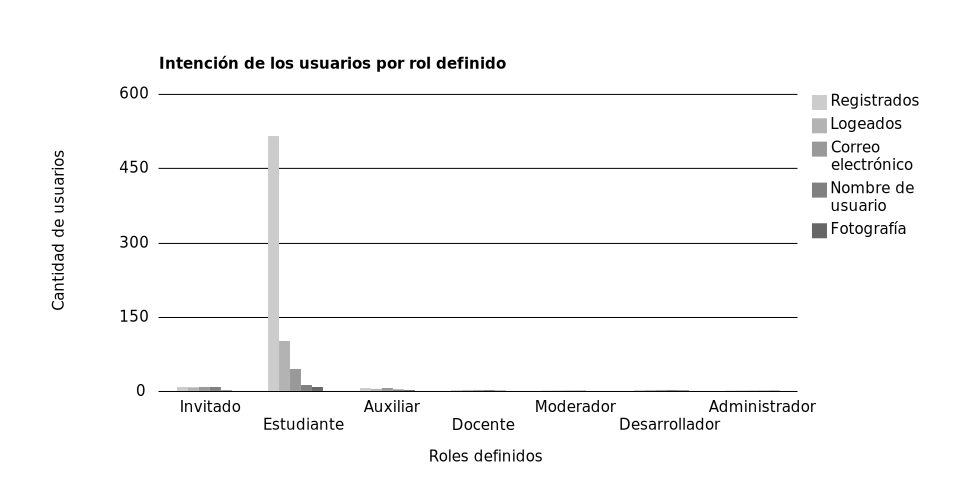
\includegraphics[width=1.0\textwidth,natwidth=960,natheight=184]{graphics/cap5_1.png}
%\caption{Intención de los usuarios clasificados por rol}
%\label{usuarios_tabla_1}
%\end{figure}

Destaca en esta tabla la disparidad entre el rol de estudiante y los demás
roles, como puede verse en la Figura \ref{usuarios_bars_1}, del conjunto de
usuarios registrados, únicamente el 20\% ingreso alguna vez al sistema, es de
rescatar además, que los usuarios fueron registrados automáticamente por sus
respectivos docentes.

%\begin{figure}
%\centering
%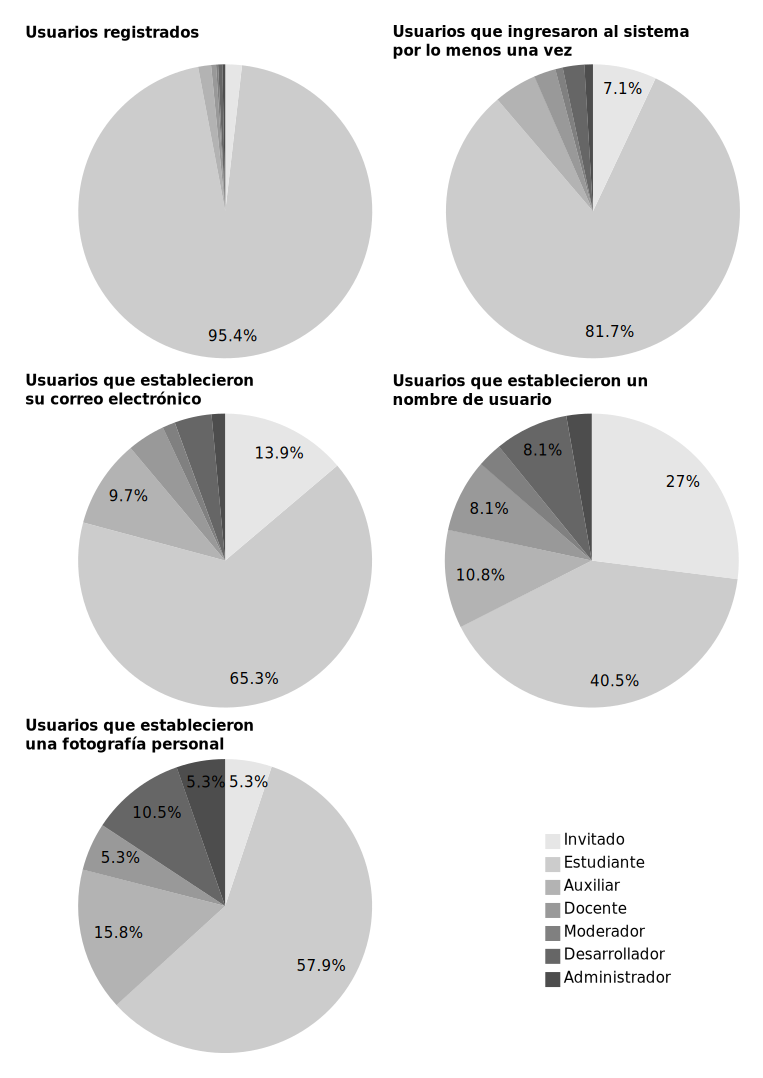
\includegraphics[width=1.0\textwidth,natwidth=956,natheight=476]{graphics/cap5_2.png}
%\caption{Diagrama de barras de la intención de los usuarios clasificados por
%rol}
%\label{usuarios_bars_1}
%\end{figure}

%Puede verse en la Figura \ref{usuarios_pie_1} como el predominio en cantidad de
%los estudiantes va decayendo progresivamente en intención frente a los otros
%roles. Considerando los escasa cantidad de atractivos que posee el sistema es
%importante considerar una audiencia de 126 personas como el primer paso hacia
%la construcción de un lugar común para el estudio realizado.\\

%Respecto a la actividad de los usuarios sobre el sistema, puede verse en la
%Figura \ref{usuarios_tabla_2} la escasisima actividad, participación y
%popularidad en todos los roles, exceptuando el de los desarrolladores. Puede
%verse también en la Figura \ref{usuarios_bars_2} el prometedor indicador de
%sociabilidad, que como puede verse en la Figura \ref{usuarios_pie_2} es el mas
%homogéneo, lo que augura una conectividad mas que deseable para los usuarios.

%\begin{figure}[H]
%\centering
%\includegraphics[scale=0.4]{graphics/usuarios_pie_1.png}
%\caption {Porcentajes de intención de los usuarios clasificados por rol}
%\label{usuarios_pie_1}
%\end{figure}

%\begin{figure}[H]
%\centering
%\includegraphics[scale=0.4]{graphics/usuarios_tabla_2.png}
%\caption {Actividad de los usuarios clasificados por rol}
%\label {usuarios_tabla_2}
%\end{figure}

%\begin{figure}[H]
%\centering
%\includegraphics[scale=0.4]{graphics/usuarios_bars_2.png}
%\caption {Diagrama de barras de la actividad de los usuarios clasificados por
%rol}
%\label {usuarios_bars_2}
%\end{figure}

%\begin{figure}[H]
%\centering
%\includegraphics[scale=0.4]{graphics/usuarios_pie_2.png}
%\caption {Porcentajes de actividad clasificados por rol}
%\label {usuarios_pie_2}
%\end{figure}

\subsection{Contactos}

%Considerando los indicadores de sociabilidad, puede apreciarse la matriz de
%adyacencias (Figura \ref{contactos_matriz}) de la red social, puede verse que
%los enlaces fuertes son casi exclusividad propia de los desarrolladores, siendo
%entre los otros roles predominantes los enlaces débiles. Puede verse también
%una sutil relación entre los usuarios que establecieron el nombre de usuario en
%su perfil, y los niveles de sociabilidad. Cuya interrelación, es motivo de
%seguimiento e intención de demostración.

%\begin{figure}[H]
%\centering
%\includegraphics[scale=0.4]{graphics/contactos_matriz.png}
%\caption {Matriz de adyacencia de la red social}
%\label {contactos_matriz}
%\end{figure}

\subsection{Espacios Virtuales}

%En la Figura \ref{espacios_tabla_1} pueden verse los distintos tipos de
%espacios virtuales y sus indicadores propios, entre los que destaca la
%supremacía del espacio portada, por sobre cualquier otro espacio, siendo el que 
%capta mas audiencia de entre los espacios. También es notorio el ausente uso de
%espacios para equipos de trabajo en los grupos, cosa que puede ser debida a las
%escasez de grupos registrados. Si bien la portada acapara la mayor audiencia,
%no acapara la mayor cantidad de recursos (Figura \ref{espacios_bars_1}),
%llevándose los espacios de comunidades un 45\% del contenido del sitio, 
%reforzando la teoría de fomento hacia los espacios menos formales (Figura
%\ref{espacios_pie_1}).

%\begin{figure}[H]
%\centering
%\includegraphics[scale=0.4]{graphics/espacios_tabla_1.png}
%\caption {Clasificación de los espacios y su actividad}
%\label {espacios_tabla_1}
%\end{figure}

%\begin{figure}[H]
%\centering
%\includegraphics[scale=0.4]{graphics/espacios_bars_1.png}
%\caption {Diagrama de barras de los espacios y sus recursos}
%\label {espacios_bars_1}
%\end{figure}

%\begin{figure}[H]
%\centering
%\includegraphics[scale=0.4]{graphics/espacios_pie_1.png}
%\caption {Porcentajes de los espacios y sus recursos seg\'un su tipo}
%\label {espacios_pie_1}
%\end{figure}

\subsection{Recursos}

%Los recursos pueden ser de varios tipos (Figura \ref{recursos_tabla_1}),
%destacando la gran cantidad de notas (Figura \ref{recursos_bars_1}) por sobre
%los otros tipos de recursos, pudiendo esto deberse a la inmensa facilidad de
%creación de estas. Aun así son las fotografías la que en proporción reciben
%mejor audiencia, y son los archivos los que reciben mayor cantidad de 
%comentarios (Figura \ref{recursos_pie_1}).

%\begin{figure}[H]
%\centering
%\includegraphics[scale=0.4]{graphics/recursos_tabla_1.png}
%\caption {Clasificación de los recursos según su tipo}
%\label {recursos_tabla_1}
%\end{figure}

%\begin{figure}[H]
%\centering
%\includegraphics[scale=0.4]{graphics/recursos_bars_1.png}
%\caption {Diagrama de barras de los recursos y sus niveles de repercusión}
%\label {recursos_bars_1}
%\end{figure}

%\begin{figure}[H]
%\centering
%\includegraphics[scale=0.4]{graphics/recursos_pie_1.png}
%\caption {Porcentajes de los recursos según su tipo}
%\label {recursos_pie_1}
%\end{figure}

\subsection{Linea de tiempo}

%Finalizados los elementos propios de la herramienta, se observan ahora las
%lineas de tiempo, donde se presentan los tiempos en los que estos elementos han
%sido creados.
%En la Figura \ref{tiempos_area_1} puede apreciarse en la linea de creación de
%los usuarios, los registros automáticos de los estudiantes, de parte del
%docente de su materia, siendo la creación de usuarios la linea predominante en
%esta gráfica.

%\begin{figure}[H]
%\centering
%\includegraphics[scale=0.25]{graphics/tiempos_area_1.png}
%\caption {Linea de tiempo de la creación de elementos en el sistema}
%\label {tiempos_area_1}
%\end{figure}

%En la Figura \ref{tiempos_area_2} resalta la curiosa relación entre las lineas
%de creación de recursos y la de creación de contactos, siendo esta la linea que
%determina todo el objeto de investigación.

%\begin{figure}[H]
%\centering
%\includegraphics[scale=0.25]{graphics/tiempos_area_2.png}
%\caption {Linea de tiempo de la creación de elementos en el sistema}
%\label {tiempos_area_2}
%\end{figure}

\section{Conclusiones}
\section{Recomendaciones}


\begin{appendix}
\chapter{Glosario de términos}

Muchos de los términos utilizados en este documento, están referidos a
conceptos que mezclan terminología de Internet, psicología, y pedagogía.
Para evitar las ambigüedades en estos términos (que son de amplio uso en el
documento) se ha creado este anexo. Estos son:

\begin{description}
\item [Usuario:] Persona que tiene el potencial de utilizar el sistema, cosa
que no implica que lo use.
\item [Rol:] Definición del conjunto de funciones del sistema, disponibles para
los usuarios.
\item [Docente:] Tipo de rol definido en el sistema, y que tiene la intención
de representar a un profesor.
\item [Espacio virtual:] Lugar del sistema donde los usuarios pueden compartir
recursos.
\item [Materia:] Tipo de espacio virtual de tipo formal, que engloba una tópico
determinado y que puede contener uno o varios grupos.
\item [Grupo:] Tipo de espacio virtual de tipo formal, que es regida por un
docente y que define una forma de enseñanza independiente de otros espacios
virtuales.
\item [Recurso:] Pieza de información creada por los usuarios, que es
compartida a todos los usuarios de un espacio virtual determinado.
\item [Actividad:] Indicador del sistema que mide el numero de recursos creados
por un usuario.
\item [Participación:] Indicador del sistema que mide el numero de comentarios
creados por un usuario.
\item [Contactos:] Usuarios del sistema que poseen algún tipo de vinculo con 
otro usuario.
\item [Enlace débil:] Es el tipo de relación entre dos usuarios, en el que solo
uno de ellos reconoce al otro.
\item [Enlace fuerte:] Es el tipo de relación entre dos usuarios, en el que 
ambos se reconocen.
\item [Sociabilidad:] Indicador del sistema que mide el numero de enlaces, ya
sean fuertes o débiles, que posee un usuario.
\item [Popularidad:] Indicador del sistema que mide el grado de valoración de 
los usuarios hacia los recursos de un usuario.
\item [Audiencia:] Es el conjunto de usuarios que únicamente vieron el recurso,
sin realizar otra acción hacia este.
\item [Calificadores:] Es el conjunto de usuarios que mostraron un interés 
explicito hacia un recurso en particular.
\end{description}

Las relaciones existentes entre los elementos del sistema están resumidos en la
Figura \ref{nomenclatura}.
\begin{figure}
\centering
\includegraphics[scale=0.3]{graphics/nomenclatura.png}
\caption {Relación entre los conceptos utilizados en el sistema}
\label {nomenclatura}
\end{figure}

\chapter{Manual de instalación}

\end{appendix}

\backmatter
\begin{thebibliography}{99}

\bibitem{Jeria} Jeria Carvajal, Esther.\\
\emph{Fenómeno Facebook.}\\
Extraído el 01 de Mayo del 2011, de\\
http://www.bibliodigital.udec.cl/index.php?option=com\_content\
\&task=view\&id=113\&Itemid=9

\bibitem{Rodriguez} Rodríguez Morales, Germania (2008, Mayo).\\
\emph{Educación Superior en Latinoamérica y la Web2.0.}\\
Extraído el 24 de Abril del 2011, de\\
http://www.utpl.edu.ec/gcblog/wp-content/uploads/web2-y-educacion-superior.pdf

\bibitem{Gonzalez} González Mariño, Julio Cesar (2006, Enero).\\
\emph{B-Learning utilizando software libre, una alternativa viable en
Educación Superior.}\\
Universidad Autónoma de Tamaulipas, México.\\
Extraído el 24 de Abril del 2011, de\\
http://revistas.ucm.es/edu/11302496/articulos/RCED0606120121A.PDF

\bibitem{Bartolome} Bartolomé, Antonio (2004).\\
\emph{Blended Learning. Conceptos básicos.}\\
Píxel-Bit. Revista de Medios y Educación, 23, pp. 7-20.\\
Universidad de Barcelona, España.\\
Extraído el 24 de Abril del 2011, de\\
http://www.lmi.ub.es/personal/bartolome/articuloshtml/\\
04\_blended\_learning/documentacion/1\_bartolome.pdf

\bibitem{Santamaria} Santamaria, Fernando.\\
\emph{Algunos apuntes sobre insignias o badges en educación.}\\
Extraído el 24 de Abril del 2011, de\\
http://fernandosantamaria.com/blog/2011/12/\\
algunos-apuntes-sobre-insignias-o-badges-en-educacion/

\bibitem{Rojas} Rojas Velásquez, Freddy (2001, Junio).\\
\emph{Enfoques sobre el aprendizaje humano.}\\
Departamento de Ciencia y Tecnología del Comportamiento.\\
Universidad Simón Bolívar.\\
Extraído el 28 de Septiembre del 2013, de\\
http://ares.unimet.edu.ve/programacion/psfase3/modII/biblio/\\
Enfoques\_sobre\_el\_aprendizaje1.pdf

\bibitem{ABC} Definición ABC.\\
\emph{Definición de conductismo.}\\
Extraído el 30 de Septiembre del 2013, de\\
http://www.definicionabc.com/general/conductismo.php\#ixzz2gQeKv5i6

\bibitem{Glez} Glez Guadarrama, Gerardo.\\
\emph{Repertorios básicos.}\\
Extraído el 30 de Septiembre del 2013, de\\
http://glosarioconductual.blogspot.com/2013/06/repertorios-basicos.html

\bibitem{Venegas} Cuco de Venegas.\\
\emph{Gamificación y SocialCRM.}\\
Extraído el 02 de Octubre del 2013, de\\
http://scrm.waplus.net/?p=44

\bibitem{LasIndias} Indianopedia.\\
\emph{Cultura de la adhesión.}\\
Extraído el 02 de Abril del 2014, de\\
http://lasindias.com/indianopedia/cultura-de-la-adhesion

\bibitem{Santamaria2} Santamaria, Fernando.\\
\emph{Las redes sociales en el ámbito educativo.}\\
Extraído el 03 de Abril del 2014, de\\
http://www.slideshare.net/lernys/las-redes-sociales-en-el-mbito-educativo

\end{thebibliography}


\end{document}
